\documentclass[twoside]{book}

% Packages required by doxygen
\usepackage{fixltx2e}
\usepackage{calc}
\usepackage{doxygen}
\usepackage[export]{adjustbox} % also loads graphicx
\usepackage{graphicx}
\usepackage[utf8]{inputenc}
\usepackage{makeidx}
\usepackage{multicol}
\usepackage{multirow}
\PassOptionsToPackage{warn}{textcomp}
\usepackage{textcomp}
\usepackage[nointegrals]{wasysym}
\usepackage[table]{xcolor}

% Font selection
\usepackage[T1]{fontenc}
\usepackage[scaled=.90]{helvet}
\usepackage{courier}
\usepackage{amssymb}
\usepackage{sectsty}
\renewcommand{\familydefault}{\sfdefault}
\allsectionsfont{%
  \fontseries{bc}\selectfont%
  \color{darkgray}%
}
\renewcommand{\DoxyLabelFont}{%
  \fontseries{bc}\selectfont%
  \color{darkgray}%
}
\newcommand{\+}{\discretionary{\mbox{\scriptsize$\hookleftarrow$}}{}{}}

% Page & text layout
\usepackage{geometry}
\geometry{%
  a4paper,%
  top=2.5cm,%
  bottom=2.5cm,%
  left=2.5cm,%
  right=2.5cm%
}
\tolerance=750
\hfuzz=15pt
\hbadness=750
\setlength{\emergencystretch}{15pt}
\setlength{\parindent}{0cm}
\setlength{\parskip}{3ex plus 2ex minus 2ex}
\makeatletter
\renewcommand{\paragraph}{%
  \@startsection{paragraph}{4}{0ex}{-1.0ex}{1.0ex}{%
    \normalfont\normalsize\bfseries\SS@parafont%
  }%
}
\renewcommand{\subparagraph}{%
  \@startsection{subparagraph}{5}{0ex}{-1.0ex}{1.0ex}{%
    \normalfont\normalsize\bfseries\SS@subparafont%
  }%
}
\makeatother

% Headers & footers
\usepackage{fancyhdr}
\pagestyle{fancyplain}
\fancyhead[LE]{\fancyplain{}{\bfseries\thepage}}
\fancyhead[CE]{\fancyplain{}{}}
\fancyhead[RE]{\fancyplain{}{\bfseries\leftmark}}
\fancyhead[LO]{\fancyplain{}{\bfseries\rightmark}}
\fancyhead[CO]{\fancyplain{}{}}
\fancyhead[RO]{\fancyplain{}{\bfseries\thepage}}
\fancyfoot[LE]{\fancyplain{}{}}
\fancyfoot[CE]{\fancyplain{}{}}
\fancyfoot[RE]{\fancyplain{}{\bfseries\scriptsize Generated by Doxygen }}
\fancyfoot[LO]{\fancyplain{}{\bfseries\scriptsize Generated by Doxygen }}
\fancyfoot[CO]{\fancyplain{}{}}
\fancyfoot[RO]{\fancyplain{}{}}
\renewcommand{\footrulewidth}{0.4pt}
\renewcommand{\chaptermark}[1]{%
  \markboth{#1}{}%
}
\renewcommand{\sectionmark}[1]{%
  \markright{\thesection\ #1}%
}

% Indices & bibliography
\usepackage{natbib}
\usepackage[titles]{tocloft}
\setcounter{tocdepth}{3}
\setcounter{secnumdepth}{5}
\makeindex

% Hyperlinks (required, but should be loaded last)
\usepackage{ifpdf}
\ifpdf
  \usepackage[pdftex,pagebackref=true]{hyperref}
\else
  \usepackage[ps2pdf,pagebackref=true]{hyperref}
\fi
\hypersetup{%
  colorlinks=true,%
  linkcolor=blue,%
  citecolor=blue,%
  unicode%
}

% Custom commands
\newcommand{\clearemptydoublepage}{%
  \newpage{\pagestyle{empty}\cleardoublepage}%
}

\usepackage{caption}
\captionsetup{labelsep=space,justification=centering,font={bf},singlelinecheck=off,skip=4pt,position=top}

%===== C O N T E N T S =====

\begin{document}

% Titlepage & ToC
\hypersetup{pageanchor=false,
             bookmarksnumbered=true,
             pdfencoding=unicode
            }
\pagenumbering{roman}
\begin{titlepage}
\vspace*{7cm}
\begin{center}%
{\Large Vespucci Library \\[1ex]\large 1.\+0.\+0 }\\
\vspace*{1cm}
{\large Generated by Doxygen 1.8.11}\\
\end{center}
\end{titlepage}
\clearemptydoublepage
\tableofcontents
\clearemptydoublepage
\pagenumbering{arabic}
\hypersetup{pageanchor=true}

%--- Begin generated contents ---
\chapter{Guidelines for Potential Contributors}
\label{md_CONTRIBUTING}
\hypertarget{md_CONTRIBUTING}{}
Thank you for your interest in contributing to the \hyperlink{namespace_vespucci}{Vespucci} Project. These guidelines should help you make a valuable contribution to the project. They cover the process of contributing to \hyperlink{namespace_vespucci}{Vespucci}, the process of adding a spectral pre-\/processing method and the process of adding a spectral analysis method. By following these guidelines, we hope \hyperlink{namespace_vespucci}{Vespucci} can attain a higher degree of quality than other research code.

\section*{Contributing to \hyperlink{namespace_vespucci}{Vespucci} }

The issues page on Git\+Hub includes features we would like to see added to \hyperlink{namespace_vespucci}{Vespucci} that we are currently not working on. If you have a contribution to make, comment on one of these issues (or start your own) and we may assign the issue to you.

If you have code to contribute to \hyperlink{namespace_vespucci}{Vespucci}, simply make a pull request with your changes to the Vespucci\+Project Git\+Hub page. The contribution should include unit tests for at least the functions added to the {\ttfamily \hyperlink{namespace_vespucci_1_1_math}{Vespucci\+::\+Math}} namespace. The pull request will be automatically built by our build service providers, which will execute unit tests (provided you have added them to the Test.\+pro project). The code will be examined for style and quality by the maintainer, and if all tests pass and the contribution is deemed within the mission of the project, your contribution will be integrated into the code base and your name added to our list of contributors. Any code contributed must compile, test, and run successfully on all three of \hyperlink{namespace_vespucci}{Vespucci}\textquotesingle{}s target platforms.

If you have already implemented a method not found in \hyperlink{namespace_vespucci}{Vespucci} in M\+A\+T\+L\+AB or Octave, take a look at the \href{http://arma.sourceforge.net/docs.html#syntax}{\tt syntax conversion table}. Re-\/writing M\+A\+T\+L\+AB code in C++ using Armadillo is fairly easy.

If you are uncomfortable with Qt, but have a meaningful math function to contribute to the library, feel free to make a contribution. The user interface can be created later. Bug fixes and code that improves performance or clarity of existing functions are also welcome.

\section*{Libraries }

Generally, code contributed to the \hyperlink{namespace_vespucci}{Vespucci} project can rely only on the following libraries\+:
\begin{DoxyItemize}
\item Qt
\item Boost
\item Armadillo
\item mlpack
\end{DoxyItemize}

If there is a compelling reason to use a different library than the ones listed above, please discuss it with us using the issues tab before you start writing code. Any library that is to be used in \hyperlink{namespace_vespucci}{Vespucci} must be regularly built and tested on Windows 7 (using M\+S\+VC and G\+CC), Mac OS 10.\+7 (Using clang), and Ubuntu 14.\+04 L\+TS (or a similar G\+N\+U/\+Linux distro, using G\+CC). If the library is not regularly tested on one of these platforms, and there is compelling reason to do so, we will set-\/up regular testing using Travis-\/\+CI and or Appveyor. As Vesucci is distributed under the terms of the G\+PL, any additional library used must use a license acceptable for G\+PL software.

\section*{Code Style }

\subsection*{Style Guides }

\hyperlink{namespace_vespucci}{Vespucci} tries to adhere to the \href{https://google.github.io/styleguide/cppguide.html}{\tt Google C++ Style Guide}. However, none of the libraries \hyperlink{namespace_vespucci}{Vespucci} links to follow this guide. Armadillo uses underscore\+\_\+case for all names and mlpack and Qt use camel\+Case for all names. The following exceptions (and perhaps others) apply\+:
\begin{DoxyItemize}
\item Source files take the extension {\ttfamily .cpp}
\item Member functions that call their member\textquotesingle{}s member functions take the same style as their member\textquotesingle{}s member function (e.\+g. if we write a function in a {\ttfamily Q\+Dialog} class that calls the {\ttfamily add\+Graph} member of a {\ttfamily \hyperlink{class_q_custom_plot}{Q\+Custom\+Plot}} object, we name the member of the {\ttfamily Q\+Dialog} \char`\"{}`add\+Graph()`\char`\"{}, rather than the stylistically preferred \char`\"{}`\+Add\+Graph()`\char`\"{}).
\end{DoxyItemize}

\subsection*{Names }


\begin{DoxyItemize}
\item Both member functions and functions that do not belong to a class are named in Pascal\+Case, unless they are getters.
\item Member variables are denoted in underscore\+\_\+case, with a trailing underscore (e.\+g. {\ttfamily name\+\_\+}, {\ttfamily spectra\+\_\+}, etc).
\item Variables that are not members are denoted in underscore\+\_\+case.
\item Setters are named in Pascal\+Case like other functions, but are named after the variables they set (e.\+g. {\ttfamily Set\+Name()} for the setter of the {\ttfamily name\+\_\+} member).
\item Getters are named after the member they return (e.\+g. the getter for {\ttfamily abscissa\+\_\+} is named {\ttfamily abscissa()}). Getters that return pointers to members have {\ttfamily \+\_\+ptr} appended to the end of their names. Where getters that return copies and getters that return references both exist, the getter that returns the reference is named with {\ttfamily \+\_\+ref} appended.
\item Every function belongs to a namespace, either the namespace of its parent class or a namespace like {\ttfamily \hyperlink{namespace_vespucci_1_1_math}{Vespucci\+::\+Math}} or {\ttfamily Binary\+Import}.
\item Widgets in Qt forms are named using Qt style inside .ui files, but use our style inside C++ classes (e.\+g. {\ttfamily name\+Line\+Edit} becomes {\ttfamily name\+\_\+line\+\_\+edit\+\_\+}). The type of the widget should be included in the name.
\item As mentioned above, an exception exists for a function whose sole purpose is to call the member of one of the class\textquotesingle{}s members.
\end{DoxyItemize}

\subsection*{Types }

Variables in \hyperlink{namespace_vespucci}{Vespucci} should use the following types\+:
\begin{DoxyItemize}
\item Numeric data should use armadillo types whenever possible.
\item Data to be displayed to the user should use Qt types whenever possible, converting them to standard library types only when necessary.
\item If a variable is expected to be unsigned, it should use an unsigned type.
\end{DoxyItemize}

\section*{Adding Processing Methods to \hyperlink{namespace_vespucci}{Vespucci} }

To add a processing method to \hyperlink{namespace_vespucci}{Vespucci}, the following must be done\+:
\begin{DoxyItemize}
\item A member function must be added to {\ttfamily \hyperlink{class_vespucci_dataset}{Vespucci\+Dataset}} to execute the analysis.
\item If the method requires more than 5 lines of code, a function performing the method must be included in the {\ttfamily \hyperlink{namespace_vespucci_1_1_math}{Vespucci\+::\+Math}} namespace in the \hyperlink{namespace_vespucci}{Vespucci} library.
\item A form class subclassed from {\ttfamily Q\+Dialog} must be created, or an existing dialog expanded to handle the new method.
\end{DoxyItemize}

\subsection*{Processing G\+UI Classes }

If a class already exists for performing a processing step substantially similar to the method to be added, the existing class should be expanded by the addition of widgets to handle user input. Widgets may also simply be reused with their {\ttfamily Q\+Label}s changed. If a new form class must be created, follow the same procedure as you would for a new analysis form class, documented in the subsection \char`\"{}\+Analysis G\+U\+I Classes\char`\"{} of the section \char`\"{}\+Adding Analysis Methods to Vespucci\char`\"{}.

\section*{Adding Analysis Methods to \hyperlink{namespace_vespucci}{Vespucci} }

To add an analysis method to \hyperlink{namespace_vespucci}{Vespucci}, the following must be done\+:
\begin{DoxyItemize}
\item A member function must be added to {\ttfamily \hyperlink{class_vespucci_dataset}{Vespucci\+Dataset}} to execute the analysis. This member must take {\ttfamily Q\+String name} as its first parameter.
\item If a method has not yet been implemented in mlpack, a function to execute the analysis must be created in the {\ttfamily \hyperlink{namespace_vespucci_1_1_math}{Vespucci\+::\+Math}} namespace of the Vespucci\+Library.
\item A class must be created to handle data generated by the analysis, unless mlpack has already done this.
\item If a method is already implemented in mlpack, the {\ttfamily \hyperlink{class_analysis_results}{Analysis\+Results}} may be constructed in the {\ttfamily \hyperlink{class_vespucci_dataset}{Vespucci\+Dataset}} member function.
\item A form class subclassed from {\ttfamily Q\+Dialog} to allow the user to enter parameters.
\end{DoxyItemize}

\subsection*{Analysis G\+UI Classes }

G\+UI classes to handle the input of parameters from the user must have the following\+:
\begin{DoxyItemize}
\item A constructor which takes the current {\ttfamily Q\+Model\+Index} from dataset tree view and obtains a {\ttfamily Q\+Shared\+Pointer$<$\hyperlink{class_vespucci_dataset}{Vespucci\+Dataset}$>$} to the dataset the analysis is to be performed on, and calls {\ttfamily find\+Child} on the required {\ttfamily Q\+Widget} members.
\item A member called {\ttfamily data\+\_\+} or {\ttfamily dataset\+\_\+} which contains a {\ttfamily Q\+Shared\+Pointer$<$\hyperlink{class_vespucci_dataset}{Vespucci\+Dataset}$>$} corresponding to the active dataset.
\item Pointers to the appropriate {\ttfamily Q\+Widget}s that interact with the user.
\item Correct names for the widgets. A {\ttfamily Q\+Widget} that is called \char`\"{}thing\+Widget\char`\"{} in the .ui file should have a pointer named {\ttfamily thing\+\_\+widget\+\_\+} in the class. Widgets are named in the conventional Qt style within forms, but in Google-\/esque style within the C++ classes. The base type of the widget must be included in the name (e.\+g. {\ttfamily name\+\_\+line\+\_\+edit\+\_\+} for the {\ttfamily Q\+Line\+Edit} object that takes string representing a name from a user).
\end{DoxyItemize}

\subsection*{{\ttfamily \hyperlink{class_vespucci_dataset}{Vespucci\+Dataset}} member functions }

Member functions to perform an analysis must do the following\+:
\begin{DoxyItemize}
\item Take the name of the object to display to the user and use as a key in {\ttfamily analysis\+\_\+results\+\_\+}.
\item Perform the analysis through a class designed to handle the analysis (either bespoke or included from mlpack)
\item Add a {\ttfamily Q\+Shared\+PointeR$<$\hyperlink{class_analysis_results}{Analysis\+Results}$>$} object to {\ttfamily analysis\+\_\+results\+\_\+} map containing the matrices generated by the analysis. This is obtained from the {\ttfamily Get\+Data()} method of the analysis handler or is initialized in the {\ttfamily \hyperlink{class_vespucci_dataset}{Vespucci\+Dataset}} member in the case of analysis methods implemented by mlpack.
\end{DoxyItemize}

\subsection*{Classes to Handle Analysis Data }

A {\ttfamily \hyperlink{class_vespucci_dataset}{Vespucci\+Dataset}} contains all analysis methods that may be called on it. Each analysis has a helper object which takes the data as a reference from the dataset. Helper objects must implement the following members\+:
\begin{DoxyItemize}
\item A constructor which takes the name of the result and relevant metadata
\item Private members of {\ttfamily arma\+::mat} type which store the results of the analysis. It is customary to use the member {\ttfamily results\+\_\+} when a matrix is returned from an analysis function, and to name these members the same as the parameters of the analysis function (remembering to add the trailing underscore used for members in \hyperlink{namespace_vespucci}{Vespucci}).
\item A method called {\ttfamily Apply()} to which is passed {\ttfamily spectra\+\_\+} and perhaps {\ttfamily abscissa\+\_\+}, along with the parameters of the analysis that are taken in the {\ttfamily \hyperlink{class_vespucci_dataset}{Vespucci\+Dataset}} analysis member function. This function calls the functions from the \hyperlink{namespace_vespucci}{Vespucci} library that are required for the analysis.
\item A method called {\ttfamily Get\+Data()}, which heap-\/allocates an {\ttfamily \hyperlink{class_analysis_results}{Analysis\+Results}} object in a {\ttfamily Q\+Shared\+Pointer} and calls the {\ttfamily Append\+Result()} method of the {\ttfamily \hyperlink{class_analysis_results}{Analysis\+Results}} object to add matrices. Each matrix should have name that constitutes a unique key, and if necessary, column headings should be provided in a {\ttfamily Q\+String\+List} for at least the first 15 columns of each matrix.
\end{DoxyItemize}

\subsection*{Analysis Functions in the {\ttfamily \hyperlink{namespace_vespucci_1_1_math}{Vespucci\+::\+Math}} Namespace }

Analysis methods must be implemented in either mlpack or armadillo, or in the {\ttfamily \hyperlink{namespace_vespucci_1_1_math}{Vespucci\+::\+Math}} namespace. A few style rules apply to this namespace that do not apply to \hyperlink{namespace_vespucci}{Vespucci} in general\+:
\begin{DoxyItemize}
\item All matrices on which operations are to be performed are to be taken as constant references {\ttfamily const arma\+::mat\&}. If the matrix itself is to be modified, the function should return a copy or include a copy as a non-\/{\ttfamily const} reference parameter.
\item The {\ttfamily using} directive should not to be used so as to avoid confusion between functions in the {\ttfamily std} and {\ttfamily arma} namespaces.
\item To ease wrapping with other languages, Qt classes are to be avoided. The equivalent C++ standard library class should be used instead (e.\+g. {\ttfamily std\+::string} instead of {\ttfamily Q\+String}). This is in contrast to the \hyperlink{namespace_vespucci}{Vespucci} G\+UI program, where Qt types are preferred.
\item Armadillo, Boost, and the standard library are the only libraries that may be used. This is intended to make the code readable by users who are only familiar with languages like M\+A\+T\+L\+AB.
\item Unit tests must be written using the Boost unit test framework.
\item Functions that check for success must have return values of type {\ttfamily bool}.
\item Each analysis that operates on single spectra must include a function that takes a single spectrum and a function that takes a column-\/major matrix of spectra. The function that takes a matrix will have the same name as the function that takes a vector, but with {\ttfamily Mat} appended to the end of the function name (e.\+g. {\ttfamily Quantify\+Peak} and {\ttfamily Quantify\+Peak\+Mat}, where {\ttfamily Quantify\+Peak} returns a {\ttfamily arma\+::rowvec} and {\ttfamily Quantify\+Peak\+Mat} returns an {\ttfamily arma\+::mat}).
\item If a matrix is expected to contain only one column, the {\ttfamily arma\+::vec} type should be used. If a matrix is expected to contain only one row, {\ttfamily arma\+::rowvec} type should be used.
\item If a value is expected to be unsigned, use {\ttfamily arma\+::uword} for integers and {\ttfamily unsigned double} for floating-\/point numbers.
\item Any function that can throw an exception should be inside of a {\ttfamily try/catch} block. The {\ttfamily catch} block must write the function call that threw the exception to {\ttfamily stdout} and throw the same exception again.
\item A function returning a matrix with more than one column for each spectrum should include these matrices in an {\ttfamily arma\+::field$<$arma\+::mat$>$} type.
\item Each function should be defined in a file with the same name as the header it is declared in and each type of analysis should include its own header and source file.
\item The use of C++11 features is highly recommended when they reduce the complexity of the code.
\end{DoxyItemize}

\section*{Writing Tests }

All methods in the \hyperlink{namespace_vespucci}{Vespucci} library are unit tested to ensure code quality and reproducibility of results. The project located in the Test folder is used to run all unit tests on math functions. Example datasets are provided, including real-\/world and generated spectra. Unit tests written for functions in the \hyperlink{namespace_vespucci}{Vespucci} library should use the Boost unit test framework. Tests written for Qt classes should use Qt\+Test. Some methods, such as Vertex Components Analysis are untestable as they produce different results each time they are run on the same data. These functions should only be tested for the validity of their output, not for the values. 
\chapter{Vespucci}
\label{md_README}
\hypertarget{md_README}{}
\href{https://ci.appveyor.com/project/dpfoose/vespucci}{\tt } \href{https://travis-ci.org/VespucciProject/Vespucci}{\tt $<$img src=\char`\"{}https\+://travis-\/ci.\+org/\+Vespucci\+Project/\+Vespucci.\+svg?branch=master\char`\"{} alt=\char`\"{}\char`\"{}Travis-\/\+CI Build Status\char`\"{}\char`\"{}/$>$} \href{https://scan.coverity.com/projects/vespucciproject-vespucci}{\tt $<$img src=\char`\"{}https\+://scan.\+coverity.\+com/projects/9309/badge.\+svg\char`\"{} alt=\char`\"{}\char`\"{}Coverity Scan Build Status\char`\"{}\char`\"{}/$>$}

\hyperlink{namespace_vespucci}{Vespucci} is a free/libre/open-\/source, cross-\/platform tool for spectroscopic imaging. \hyperlink{namespace_vespucci}{Vespucci} is regularly built on Windows, Mac and Linux operating systems.

\hyperlink{namespace_vespucci}{Vespucci} is distributed under the terms of the G\+NU General Public License version 3. A copy of this license is provided in L\+I\+C\+E\+N\+SE

A research article detailing \hyperlink{namespace_vespucci}{Vespucci} has been published in the \href{http://openresearchsoftware.metajnl.com/articles/10.5334/jors.91/}{\tt {\itshape Journal of Open Research Software}}

This branch is the active branch of the project and, while more stable than the branches of individual contributors, is {\bfseries probably not stable}.

After the release of the first 1.\+0.\+0 beta, there will be tags established for releases.

Bug reports should be directed to the Issues tab.

\subsection*{Binary Releases\+: }

Releases for all three supported platforms are availible in the Releases tab. The latest binaries are available at \href{https://bintray.com/vespucciproject/Vespucci_automated_builds/Vespucci_latest}{\tt Bintray} The release package includes the executable, the \hyperlink{namespace_vespucci}{Vespucci} library and runtime pre-\/requisites and the header files needed to use the library. \subsection*{Versioning\+: }

Versions up to 1.\+0.\+0 are not considered stable and changes between 0.\+n.\+0 and 0.\+n+1.0 may be major. After 1.\+0.\+0, 1.\+n+1.0 will contain new features to 1.\+n.\+0, but will have an A\+PI that is mostly compatible. n+1.0.\+0 contains major changes in the A\+PI that may break programs built from it. 1.\+n.\+x+1 contains a bug fix or minor improvement to 1.\+n.\+x

\subsection*{Compiling \hyperlink{namespace_vespucci}{Vespucci}\+: }

Compiling \hyperlink{namespace_vespucci}{Vespucci} from source is not the easiest but still possible. Look at .travis.\+yml for linux and mac builds and appveyor.\+yml for windows builds.

\hyperlink{namespace_vespucci}{Vespucci} has the following prerequisites\+:
\begin{DoxyItemize}
\item Qt 5.\+5+
\item Armadillo (with B\+L\+A\+S/\+L\+A\+P\+A\+CK and H\+D\+F5)
\item mlpack
\item yaml-\/cpp
\item quazip
\end{DoxyItemize}

Look at the scripts used by .travis.\+yml and appveyor.\+yml to figure out how to build on your platform.

\subsection*{Contributing\+: }

If you would like to contribute to \hyperlink{namespace_vespucci}{Vespucci}, please read \hyperlink{_c_o_n_t_r_i_b_u_t_i_n_g_8md_source}{C\+O\+N\+T\+R\+I\+B\+U\+T\+I\+N\+G.\+md} If you need help setting up your development environment to build \hyperlink{namespace_vespucci}{Vespucci} from source, feel free to contact us. 
\chapter{Namespace Index}
\section{Namespace List}
Here is a list of all documented namespaces with brief descriptions\+:\begin{DoxyCompactList}
\item\contentsline{section}{\hyperlink{namespace_vespucci}{Vespucci} \\*A namespace for \char`\"{}global\char`\"{} functions, including math functions }{\pageref{namespace_vespucci}}{}
\item\contentsline{section}{\hyperlink{namespace_vespucci_1_1_math}{Vespucci\+::\+Math} \\*A namespace for math functions relating to linear least squares regression }{\pageref{namespace_vespucci_1_1_math}}{}
\item\contentsline{section}{\hyperlink{namespace_vespucci_1_1_math_1_1_dimension_reduction}{Vespucci\+::\+Math\+::\+Dimension\+Reduction} \\*A namespace for math functions relating to dimension reduction }{\pageref{namespace_vespucci_1_1_math_1_1_dimension_reduction}}{}
\item\contentsline{section}{\hyperlink{namespace_vespucci_1_1_math_1_1_fitting}{Vespucci\+::\+Math\+::\+Fitting} \\*A namespace for math functions relating to non-\/linear curve fitting }{\pageref{namespace_vespucci_1_1_math_1_1_fitting}}{}
\item\contentsline{section}{\hyperlink{namespace_vespucci_1_1_math_1_1_normalization}{Vespucci\+::\+Math\+::\+Normalization} \\*A namespace for math functions relating to normalization }{\pageref{namespace_vespucci_1_1_math_1_1_normalization}}{}
\item\contentsline{section}{\hyperlink{namespace_vespucci_1_1_math_1_1_peak_finding}{Vespucci\+::\+Math\+::\+Peak\+Finding} \\*A namespace for math functions relating to peak detection and counting }{\pageref{namespace_vespucci_1_1_math_1_1_peak_finding}}{}
\item\contentsline{section}{\hyperlink{namespace_vespucci_1_1_math_1_1_quantification}{Vespucci\+::\+Math\+::\+Quantification} \\*A namespace for math functions relating to peak quantification }{\pageref{namespace_vespucci_1_1_math_1_1_quantification}}{}
\item\contentsline{section}{\hyperlink{namespace_vespucci_1_1_math_1_1_smoothing}{Vespucci\+::\+Math\+::\+Smoothing} \\*A namespace for math functions relating to filtering and smoothing signals }{\pageref{namespace_vespucci_1_1_math_1_1_smoothing}}{}
\end{DoxyCompactList}

\chapter{Hierarchical Index}
\section{Class Hierarchy}
This inheritance list is sorted roughly, but not completely, alphabetically\+:\begin{DoxyCompactList}
\item \contentsline{section}{Analysis\+Results}{\pageref{class_analysis_results}}{}
\begin{DoxyCompactList}
\item \contentsline{section}{Mlpack\+P\+C\+A\+Data}{\pageref{class_mlpack_p_c_a_data}}{}
\item \contentsline{section}{P\+L\+S\+Data}{\pageref{class_p_l_s_data}}{}
\item \contentsline{section}{Principal\+Components\+Data}{\pageref{class_principal_components_data}}{}
\item \contentsline{section}{Univariate\+Data}{\pageref{class_univariate_data}}{}
\item \contentsline{section}{V\+C\+A\+Data}{\pageref{class_v_c_a_data}}{}
\end{DoxyCompactList}
\item \contentsline{section}{Q\+C\+P\+Axis\+Painter\+Private\+:\+:Cached\+Label}{\pageref{struct_q_c_p_axis_painter_private_1_1_cached_label}}{}
\item \contentsline{section}{Vespucci\+:\+:External\+:\+:data\+\_\+object}{\pageref{class_vespucci_1_1_external_1_1data__object}}{}
\item \contentsline{section}{Data\+Model}{\pageref{class_data_model}}{}
\item \contentsline{section}{Dataset\+Loader}{\pageref{class_dataset_loader}}{}
\item \contentsline{section}{Dataset\+Saver}{\pageref{class_dataset_saver}}{}
\item \contentsline{section}{Vespucci\+:\+:Math\+:\+:Distance\+Metric\+Wrapper}{\pageref{class_vespucci_1_1_math_1_1_distance_metric_wrapper}}{}
\item \contentsline{section}{Vespucci\+:\+:External\+:\+:File\+Interprocess}{\pageref{class_vespucci_1_1_external_1_1_file_interprocess}}{}
\item \contentsline{section}{Vespucci\+:\+:External\+:\+:Interprocess\+Sender}{\pageref{class_vespucci_1_1_external_1_1_interprocess_sender}}{}
\item \contentsline{section}{Macro\+Parser}{\pageref{class_macro_parser}}{}
\item \contentsline{section}{Map\+Data}{\pageref{class_map_data}}{}
\item Q\+Abstract\+Item\+Model\begin{DoxyCompactList}
\item \contentsline{section}{Dataset\+Tree\+Model}{\pageref{class_dataset_tree_model}}{}
\end{DoxyCompactList}
\item Q\+Abstract\+List\+Model\begin{DoxyCompactList}
\item \contentsline{section}{Dataset\+List\+Model}{\pageref{class_dataset_list_model}}{}
\item \contentsline{section}{Map\+List\+Model}{\pageref{class_map_list_model}}{}
\end{DoxyCompactList}
\item Q\+Abstract\+Table\+Model\begin{DoxyCompactList}
\item \contentsline{section}{Spectra\+Table\+Model}{\pageref{class_spectra_table_model}}{}
\item \contentsline{section}{Vespucci\+Table\+Model}{\pageref{class_vespucci_table_model}}{}
\end{DoxyCompactList}
\item \contentsline{section}{Q\+C\+P\+Axis\+Painter\+Private}{\pageref{class_q_c_p_axis_painter_private}}{}
\item \contentsline{section}{Q\+C\+P\+Bar\+Data}{\pageref{class_q_c_p_bar_data}}{}
\item \contentsline{section}{Q\+C\+P\+Color\+Gradient}{\pageref{class_q_c_p_color_gradient}}{}
\item \contentsline{section}{Q\+C\+P\+Color\+Map\+Data}{\pageref{class_q_c_p_color_map_data}}{}
\item \contentsline{section}{Q\+C\+P\+Curve\+Data}{\pageref{class_q_c_p_curve_data}}{}
\item \contentsline{section}{Q\+C\+P\+Data}{\pageref{class_q_c_p_data}}{}
\item \contentsline{section}{Q\+C\+P\+Financial\+Data}{\pageref{class_q_c_p_financial_data}}{}
\item \contentsline{section}{Q\+C\+P\+Item\+Anchor}{\pageref{class_q_c_p_item_anchor}}{}
\begin{DoxyCompactList}
\item \contentsline{section}{Q\+C\+P\+Item\+Position}{\pageref{class_q_c_p_item_position}}{}
\end{DoxyCompactList}
\item \contentsline{section}{Q\+C\+P\+Line\+Ending}{\pageref{class_q_c_p_line_ending}}{}
\item \contentsline{section}{Q\+C\+P\+Range}{\pageref{class_q_c_p_range}}{}
\item \contentsline{section}{Q\+C\+P\+Scatter\+Style}{\pageref{class_q_c_p_scatter_style}}{}
\item Q\+Dialog\begin{DoxyCompactList}
\item \contentsline{section}{About\+Dialog}{\pageref{class_about_dialog}}{}
\item \contentsline{section}{Abscissa\+Interpolation\+Dialog}{\pageref{class_abscissa_interpolation_dialog}}{}
\item \contentsline{section}{Abscissa\+Transform\+Dialog}{\pageref{class_abscissa_transform_dialog}}{}
\item \contentsline{section}{Band\+Ratio\+Dialog}{\pageref{class_band_ratio_dialog}}{}
\item \contentsline{section}{Baseline\+Dialog}{\pageref{class_baseline_dialog}}{}
\item \contentsline{section}{Booleanize\+Dialog}{\pageref{class_booleanize_dialog}}{}
\item \contentsline{section}{Bulk\+Conversion\+Dialog}{\pageref{class_bulk_conversion_dialog}}{}
\item \contentsline{section}{Citation\+Dialog}{\pageref{class_citation_dialog}}{}
\item \contentsline{section}{Classical\+Least\+Squares\+Dialog}{\pageref{class_classical_least_squares_dialog}}{}
\item \contentsline{section}{Crop\+Dialog}{\pageref{class_crop_dialog}}{}
\item \contentsline{section}{Data\+Extractor\+Dialog}{\pageref{class_data_extractor_dialog}}{}
\item \contentsline{section}{Data\+Viewer}{\pageref{class_data_viewer}}{}
\item \contentsline{section}{Filter\+Dialog}{\pageref{class_filter_dialog}}{}
\item \contentsline{section}{Fourier\+Transform\+Dialog}{\pageref{class_fourier_transform_dialog}}{}
\item \contentsline{section}{K\+Means\+Dialog}{\pageref{class_k_means_dialog}}{}
\item \contentsline{section}{Load\+Dataset}{\pageref{class_load_dataset}}{}
\item \contentsline{section}{Macro\+Dialog}{\pageref{class_macro_dialog}}{}
\item \contentsline{section}{Map\+Dialog}{\pageref{class_map_dialog}}{}
\item \contentsline{section}{Meta\+Dataset\+Dialog}{\pageref{class_meta_dataset_dialog}}{}
\item \contentsline{section}{Multi\+Import\+Dialog}{\pageref{class_multi_import_dialog}}{}
\item \contentsline{section}{Plot\+Maker\+Dialog}{\pageref{class_plot_maker_dialog}}{}
\item \contentsline{section}{Plot\+Viewer}{\pageref{class_plot_viewer}}{}
\item \contentsline{section}{P\+L\+S\+Dialog}{\pageref{class_p_l_s_dialog}}{}
\item \contentsline{section}{Principal\+Components\+Dialog}{\pageref{class_principal_components_dialog}}{}
\item \contentsline{section}{Python\+Shell\+Dialog}{\pageref{class_python_shell_dialog}}{}
\item \contentsline{section}{Range\+Dialog}{\pageref{class_range_dialog}}{}
\item \contentsline{section}{Report\+Message\+Dialog}{\pageref{class_report_message_dialog}}{}
\item \contentsline{section}{Scale\+Bar\+Dialog}{\pageref{class_scale_bar_dialog}}{}
\item \contentsline{section}{Script\+Dialog}{\pageref{class_script_dialog}}{}
\item \contentsline{section}{Settings\+Dialog}{\pageref{class_settings_dialog}}{}
\item \contentsline{section}{Spectrum\+Selection\+Dialog}{\pageref{class_spectrum_selection_dialog}}{}
\item \contentsline{section}{Spectrum\+Viewer}{\pageref{class_spectrum_viewer}}{}
\item \contentsline{section}{Stats\+Dialog}{\pageref{class_stats_dialog}}{}
\item \contentsline{section}{Stitch\+Import\+Dialog}{\pageref{class_stitch_import_dialog}}{}
\item \contentsline{section}{Threshold\+Dialog}{\pageref{class_threshold_dialog}}{}
\item \contentsline{section}{Transform\+Dialog}{\pageref{class_transform_dialog}}{}
\item \contentsline{section}{Univariate\+Dialog}{\pageref{class_univariate_dialog}}{}
\item \contentsline{section}{V\+C\+A\+Dialog}{\pageref{class_v_c_a_dialog}}{}
\end{DoxyCompactList}
\item Q\+Main\+Window\begin{DoxyCompactList}
\item \contentsline{section}{Main\+Window}{\pageref{class_main_window}}{}
\item \contentsline{section}{Map\+Viewer}{\pageref{class_map_viewer}}{}
\end{DoxyCompactList}
\item Q\+Object\begin{DoxyCompactList}
\item \contentsline{section}{Q\+C\+P\+Bars\+Group}{\pageref{class_q_c_p_bars_group}}{}
\item \contentsline{section}{Q\+C\+P\+Layer}{\pageref{class_q_c_p_layer}}{}
\item \contentsline{section}{Q\+C\+P\+Layerable}{\pageref{class_q_c_p_layerable}}{}
\begin{DoxyCompactList}
\item \contentsline{section}{Q\+C\+P\+Abstract\+Item}{\pageref{class_q_c_p_abstract_item}}{}
\begin{DoxyCompactList}
\item \contentsline{section}{Q\+C\+P\+Item\+Bracket}{\pageref{class_q_c_p_item_bracket}}{}
\item \contentsline{section}{Q\+C\+P\+Item\+Curve}{\pageref{class_q_c_p_item_curve}}{}
\item \contentsline{section}{Q\+C\+P\+Item\+Ellipse}{\pageref{class_q_c_p_item_ellipse}}{}
\item \contentsline{section}{Q\+C\+P\+Item\+Line}{\pageref{class_q_c_p_item_line}}{}
\item \contentsline{section}{Q\+C\+P\+Item\+Pixmap}{\pageref{class_q_c_p_item_pixmap}}{}
\item \contentsline{section}{Q\+C\+P\+Item\+Rect}{\pageref{class_q_c_p_item_rect}}{}
\item \contentsline{section}{Q\+C\+P\+Item\+Straight\+Line}{\pageref{class_q_c_p_item_straight_line}}{}
\item \contentsline{section}{Q\+C\+P\+Item\+Text}{\pageref{class_q_c_p_item_text}}{}
\item \contentsline{section}{Q\+C\+P\+Item\+Tracer}{\pageref{class_q_c_p_item_tracer}}{}
\end{DoxyCompactList}
\item \contentsline{section}{Q\+C\+P\+Abstract\+Plottable}{\pageref{class_q_c_p_abstract_plottable}}{}
\begin{DoxyCompactList}
\item \contentsline{section}{Q\+C\+P\+Bars}{\pageref{class_q_c_p_bars}}{}
\item \contentsline{section}{Q\+C\+P\+Color\+Map}{\pageref{class_q_c_p_color_map}}{}
\item \contentsline{section}{Q\+C\+P\+Curve}{\pageref{class_q_c_p_curve}}{}
\item \contentsline{section}{Q\+C\+P\+Financial}{\pageref{class_q_c_p_financial}}{}
\item \contentsline{section}{Q\+C\+P\+Graph}{\pageref{class_q_c_p_graph}}{}
\item \contentsline{section}{Q\+C\+P\+Statistical\+Box}{\pageref{class_q_c_p_statistical_box}}{}
\end{DoxyCompactList}
\item \contentsline{section}{Q\+C\+P\+Axis}{\pageref{class_q_c_p_axis}}{}
\item \contentsline{section}{Q\+C\+P\+Grid}{\pageref{class_q_c_p_grid}}{}
\item \contentsline{section}{Q\+C\+P\+Layout\+Element}{\pageref{class_q_c_p_layout_element}}{}
\begin{DoxyCompactList}
\item \contentsline{section}{Q\+C\+P\+Abstract\+Legend\+Item}{\pageref{class_q_c_p_abstract_legend_item}}{}
\begin{DoxyCompactList}
\item \contentsline{section}{Q\+C\+P\+Plottable\+Legend\+Item}{\pageref{class_q_c_p_plottable_legend_item}}{}
\end{DoxyCompactList}
\item \contentsline{section}{Q\+C\+P\+Axis\+Rect}{\pageref{class_q_c_p_axis_rect}}{}
\begin{DoxyCompactList}
\item \contentsline{section}{Q\+C\+P\+Color\+Scale\+Axis\+Rect\+Private}{\pageref{class_q_c_p_color_scale_axis_rect_private}}{}
\end{DoxyCompactList}
\item \contentsline{section}{Q\+C\+P\+Color\+Scale}{\pageref{class_q_c_p_color_scale}}{}
\item \contentsline{section}{Q\+C\+P\+Layout}{\pageref{class_q_c_p_layout}}{}
\begin{DoxyCompactList}
\item \contentsline{section}{Q\+C\+P\+Layout\+Grid}{\pageref{class_q_c_p_layout_grid}}{}
\begin{DoxyCompactList}
\item \contentsline{section}{Q\+C\+P\+Legend}{\pageref{class_q_c_p_legend}}{}
\end{DoxyCompactList}
\item \contentsline{section}{Q\+C\+P\+Layout\+Inset}{\pageref{class_q_c_p_layout_inset}}{}
\end{DoxyCompactList}
\item \contentsline{section}{Q\+C\+P\+Plot\+Title}{\pageref{class_q_c_p_plot_title}}{}
\end{DoxyCompactList}
\end{DoxyCompactList}
\item \contentsline{section}{Q\+C\+P\+Margin\+Group}{\pageref{class_q_c_p_margin_group}}{}
\item \contentsline{section}{Test\+Data\+Model}{\pageref{class_test_data_model}}{}
\item \contentsline{section}{Test\+Dataset}{\pageref{class_test_dataset}}{}
\item \contentsline{section}{Test\+File\+IO}{\pageref{class_test_file_i_o}}{}
\item \contentsline{section}{Test\+Fitting}{\pageref{class_test_fitting}}{}
\item \contentsline{section}{Test\+Helpers}{\pageref{class_test_helpers}}{}
\item \contentsline{section}{Test\+Normalization}{\pageref{class_test_normalization}}{}
\item \contentsline{section}{Test\+Peak\+Finding}{\pageref{class_test_peak_finding}}{}
\item \contentsline{section}{Test\+Quantification}{\pageref{class_test_quantification}}{}
\item \contentsline{section}{Test\+Smoothing}{\pageref{class_test_smoothing}}{}
\item \contentsline{section}{Test\+Workspace}{\pageref{class_test_workspace}}{}
\end{DoxyCompactList}
\item Q\+Painter\begin{DoxyCompactList}
\item \contentsline{section}{Q\+C\+P\+Painter}{\pageref{class_q_c_p_painter}}{}
\end{DoxyCompactList}
\item Q\+Widget\begin{DoxyCompactList}
\item \contentsline{section}{Data\+Widget}{\pageref{class_data_widget}}{}
\item \contentsline{section}{Plot\+Widget}{\pageref{class_plot_widget}}{}
\item \contentsline{section}{Q\+Custom\+Plot}{\pageref{class_q_custom_plot}}{}
\end{DoxyCompactList}
\item \contentsline{section}{Test\+Session}{\pageref{class_test_session}}{}
\item \contentsline{section}{Q\+C\+P\+Axis\+Painter\+Private\+:\+:Tick\+Label\+Data}{\pageref{struct_q_c_p_axis_painter_private_1_1_tick_label_data}}{}
\item \contentsline{section}{Tree\+Item}{\pageref{class_tree_item}}{}
\item \contentsline{section}{Vespucci\+Dataset}{\pageref{class_vespucci_dataset}}{}
\begin{DoxyCompactList}
\item \contentsline{section}{Meta\+Dataset}{\pageref{class_meta_dataset}}{}
\end{DoxyCompactList}
\item \contentsline{section}{Vespucci\+Workspace}{\pageref{class_vespucci_workspace}}{}
\end{DoxyCompactList}

\chapter{Class Index}
\section{Class List}
Here are the classes, structs, unions and interfaces with brief descriptions\+:\begin{DoxyCompactList}
\item\contentsline{section}{\hyperlink{class_about_dialog}{About\+Dialog} \\*The \hyperlink{class_about_dialog}{About\+Dialog} class A Q\+Dialog that displays information about \hyperlink{namespace_vespucci}{Vespucci} }{\pageref{class_about_dialog}}{}
\item\contentsline{section}{\hyperlink{class_analysis_dialog}{Analysis\+Dialog} }{\pageref{class_analysis_dialog}}{}
\item\contentsline{section}{\hyperlink{class_analysis_results}{Analysis\+Results} \\*The \hyperlink{class_analysis_results}{Analysis\+Results} class A container for a mat object that allows a mat to be copied to a heap-\/allocated object (this) so pointers to that mat cannot go out of scope. These objects should be heap-\/allocated inside smart pointers }{\pageref{class_analysis_results}}{}
\item\contentsline{section}{\hyperlink{class_band_ratio_dialog}{Band\+Ratio\+Dialog} \\*The \hyperlink{class_band_ratio_dialog}{Band\+Ratio\+Dialog} class The dialog that allows the user to create a band-\/ratio map }{\pageref{class_band_ratio_dialog}}{}
\item\contentsline{section}{\hyperlink{class_baseline_dialog}{Baseline\+Dialog} \\*The \hyperlink{class_baseline_dialog}{Baseline\+Dialog} class The dialog that allows the user to baseline-\/correct the data }{\pageref{class_baseline_dialog}}{}
\item\contentsline{section}{\hyperlink{class_booleanize_dialog}{Booleanize\+Dialog} }{\pageref{class_booleanize_dialog}}{}
\item\contentsline{section}{\hyperlink{class_citation_dialog}{Citation\+Dialog} \\*The \hyperlink{class_citation_dialog}{Citation\+Dialog} class The dialog that displays how to cite \hyperlink{namespace_vespucci}{Vespucci} }{\pageref{class_citation_dialog}}{}
\item\contentsline{section}{\hyperlink{class_crop_dialog}{Crop\+Dialog} \\*The \hyperlink{class_crop_dialog}{Crop\+Dialog} class A dialog that allows the user to \char`\"{}\+Crop\char`\"{} the dataset (delete all spectra that are outside of a chosen spatial range) }{\pageref{class_crop_dialog}}{}
\item\contentsline{section}{\hyperlink{class_c_w_t_data}{C\+W\+T\+Data} }{\pageref{class_c_w_t_data}}{}
\item\contentsline{section}{\hyperlink{class_vespucci_1_1_math_1_1_c_w_t_ridge}{Vespucci\+::\+Math\+::\+C\+W\+T\+Ridge} }{\pageref{class_vespucci_1_1_math_1_1_c_w_t_ridge}}{}
\item\contentsline{section}{\hyperlink{class_data_extractor_dialog}{Data\+Extractor\+Dialog} \\*The \hyperlink{class_data_extractor_dialog}{Data\+Extractor\+Dialog} class A dialog that allows the user to create a new dataset from a map, based on map values }{\pageref{class_data_extractor_dialog}}{}
\item\contentsline{section}{\hyperlink{class_dataset_list_model}{Dataset\+List\+Model} \\*Exposes the U\+I to the contents of the master dataset list }{\pageref{class_dataset_list_model}}{}
\item\contentsline{section}{\hyperlink{class_data_viewer}{Data\+Viewer} \\*The \hyperlink{class_data_viewer}{Data\+Viewer} class Window that displays dataset elements in a Q\+Table\+View widget }{\pageref{class_data_viewer}}{}
\item\contentsline{section}{\hyperlink{class_filter_dialog}{Filter\+Dialog} \\*The \hyperlink{class_filter_dialog}{Filter\+Dialog} class This dialog allows the user to apply filtering, smoothing or derivatization to the dataset }{\pageref{class_filter_dialog}}{}
\item\contentsline{section}{\hyperlink{class_has_peaks_dialog}{Has\+Peaks\+Dialog} }{\pageref{class_has_peaks_dialog}}{}
\item\contentsline{section}{\hyperlink{class_k_means_dialog}{K\+Means\+Dialog} \\*The \hyperlink{class_k_means_dialog}{K\+Means\+Dialog} class Allows the user to create a k-\/means clustering map }{\pageref{class_k_means_dialog}}{}
\item\contentsline{section}{\hyperlink{class_load_dataset}{Load\+Dataset} \\*The \hyperlink{class_load_dataset}{Load\+Dataset} class Dialog that allows the user to import files into the program }{\pageref{class_load_dataset}}{}
\item\contentsline{section}{\hyperlink{class_main_window}{Main\+Window} \\*The \hyperlink{class_main_window}{Main\+Window} class The main window of the program, this is where the user performs most operations }{\pageref{class_main_window}}{}
\item\contentsline{section}{\hyperlink{class_map_data}{Map\+Data} \\*The \hyperlink{class_map_data}{Map\+Data} class Class for processed map data. Images are created from this data }{\pageref{class_map_data}}{}
\item\contentsline{section}{\hyperlink{class_map_list_model}{Map\+List\+Model} \\*Exposes the U\+I to the contents of the master map list }{\pageref{class_map_list_model}}{}
\item\contentsline{section}{\hyperlink{class_map_viewer}{Map\+Viewer} \\*The \hyperlink{class_map_viewer}{Map\+Viewer} class Displays the image created by \hyperlink{class_map_data}{Map\+Data} }{\pageref{class_map_viewer}}{}
\item\contentsline{section}{\hyperlink{class_meta_dataset}{Meta\+Dataset} \\*The \hyperlink{class_meta_dataset}{Meta\+Dataset} class A subclass of \hyperlink{class_vespucci_dataset}{Vespucci\+Dataset} for datasets created from multiple other datasets. this stores information about the parents }{\pageref{class_meta_dataset}}{}
\item\contentsline{section}{\hyperlink{class_meta_dataset_dialog}{Meta\+Dataset\+Dialog} }{\pageref{class_meta_dataset_dialog}}{}
\item\contentsline{section}{\hyperlink{class_m_l_p_a_c_k_p_c_a_data}{M\+L\+P\+A\+C\+K\+P\+C\+A\+Data} }{\pageref{class_m_l_p_a_c_k_p_c_a_data}}{}
\item\contentsline{section}{\hyperlink{class_multi_import_dialog}{Multi\+Import\+Dialog} }{\pageref{class_multi_import_dialog}}{}
\item\contentsline{section}{\hyperlink{class_peak_finding_dialog}{Peak\+Finding\+Dialog} }{\pageref{class_peak_finding_dialog}}{}
\item\contentsline{section}{\hyperlink{class_plot_maker_dialog}{Plot\+Maker\+Dialog} }{\pageref{class_plot_maker_dialog}}{}
\item\contentsline{section}{\hyperlink{class_plot_viewer}{Plot\+Viewer} \\*The \hyperlink{class_plot_viewer}{Plot\+Viewer} class For displaying plots that are not maps or spectra (P\+C\+A/\+V\+C\+A/\+P\+L\+S Scatterplots, especially for meta datasets) }{\pageref{class_plot_viewer}}{}
\item\contentsline{section}{\hyperlink{class_p_l_s_data}{P\+L\+S\+Data} \\*The \hyperlink{class_p_l_s_data}{P\+L\+S\+Data} class A class for performing and storing data related to partial least squares determinant analysis }{\pageref{class_p_l_s_data}}{}
\item\contentsline{section}{\hyperlink{class_p_l_s_dialog}{P\+L\+S\+Dialog} \\*The \hyperlink{class_p_l_s_dialog}{P\+L\+S\+Dialog} class Dialog that allows the user to perform P\+L\+S determinant analysis }{\pageref{class_p_l_s_dialog}}{}
\item\contentsline{section}{\hyperlink{class_principal_components_data}{Principal\+Components\+Data} \\*The \hyperlink{class_principal_components_data}{Principal\+Components\+Data} class A class for performing and storing data from principal components analysis }{\pageref{class_principal_components_data}}{}
\item\contentsline{section}{\hyperlink{class_principal_components_dialog}{Principal\+Components\+Dialog} \\*The \hyperlink{class_principal_components_dialog}{Principal\+Components\+Dialog} class Dialog for performing principal components analysis }{\pageref{class_principal_components_dialog}}{}
\item\contentsline{section}{\hyperlink{class_range_dialog}{Range\+Dialog} \\*The \hyperlink{class_range_dialog}{Range\+Dialog} class }{\pageref{class_range_dialog}}{}
\item\contentsline{section}{\hyperlink{class_scale_bar_dialog}{Scale\+Bar\+Dialog} \\*The \hyperlink{class_scale_bar_dialog}{Scale\+Bar\+Dialog} class Dialog for the user to create a scale bar on the image }{\pageref{class_scale_bar_dialog}}{}
\item\contentsline{section}{\hyperlink{class_script_dialog}{Script\+Dialog} }{\pageref{class_script_dialog}}{}
\item\contentsline{section}{\hyperlink{class_spectra_table_model}{Spectra\+Table\+Model} }{\pageref{class_spectra_table_model}}{}
\item\contentsline{section}{\hyperlink{class_spectrum_selection_dialog}{Spectrum\+Selection\+Dialog} }{\pageref{class_spectrum_selection_dialog}}{}
\item\contentsline{section}{\hyperlink{class_spectrum_viewer}{Spectrum\+Viewer} \\*The \hyperlink{class_spectrum_viewer}{Spectrum\+Viewer} class A class for displaying spectra }{\pageref{class_spectrum_viewer}}{}
\item\contentsline{section}{\hyperlink{class_stats_dialog}{Stats\+Dialog} }{\pageref{class_stats_dialog}}{}
\item\contentsline{section}{\hyperlink{class_threshold_dialog}{Threshold\+Dialog} }{\pageref{class_threshold_dialog}}{}
\item\contentsline{section}{\hyperlink{class_univariate_analysis_dialog}{Univariate\+Analysis\+Dialog} }{\pageref{class_univariate_analysis_dialog}}{}
\item\contentsline{section}{\hyperlink{class_univariate_data}{Univariate\+Data} }{\pageref{class_univariate_data}}{}
\item\contentsline{section}{\hyperlink{class_univariate_dialog}{Univariate\+Dialog} \\*The \hyperlink{class_univariate_dialog}{Univariate\+Dialog} class Class allowing user to create univariate images }{\pageref{class_univariate_dialog}}{}
\item\contentsline{section}{\hyperlink{class_v_c_a_data}{V\+C\+A\+Data} \\*The \hyperlink{class_v_c_a_data}{V\+C\+A\+Data} class A class for performing and storing data from Vertex Components Analysis }{\pageref{class_v_c_a_data}}{}
\item\contentsline{section}{\hyperlink{class_v_c_a_dialog}{V\+C\+A\+Dialog} \\*The \hyperlink{class_v_c_a_dialog}{V\+C\+A\+Dialog} class A dialog that allows the user to perform vertex components analysis }{\pageref{class_v_c_a_dialog}}{}
\item\contentsline{section}{\hyperlink{class_vespucci_dataset}{Vespucci\+Dataset} \\*The \hyperlink{class_vespucci_dataset}{Vespucci\+Dataset} class This is the main class for dealing with hyperspectral data. This handles the import and export of spectra, and the creation of maps. Images are handled by the \hyperlink{class_map_data}{Map\+Data} class }{\pageref{class_vespucci_dataset}}{}
\item\contentsline{section}{\hyperlink{class_vespucci_r}{Vespucci\+R} }{\pageref{class_vespucci_r}}{}
\item\contentsline{section}{\hyperlink{class_vespucci_table_model}{Vespucci\+Table\+Model} \\*The \hyperlink{class_vespucci_table_model}{Vespucci\+Table\+Model} class The Q\+Abstract\+Table\+Model that handles armadillo objects for the \hyperlink{class_data_viewer}{Data\+Viewer} class }{\pageref{class_vespucci_table_model}}{}
\item\contentsline{section}{\hyperlink{class_vespucci_workspace}{Vespucci\+Workspace} \\*The \hyperlink{class_vespucci_workspace}{Vespucci\+Workspace} class A class which contains all \char`\"{}global variables\char`\"{} (that aren't held in \hyperlink{class_main_window}{Main\+Window}) }{\pageref{class_vespucci_workspace}}{}
\end{DoxyCompactList}

\chapter{File Index}
\section{File List}
Here is a list of all documented files with brief descriptions\+:\begin{DoxyCompactList}
\item\contentsline{section}{A\+P\+I\+Examples/\+Batch\+V\+C\+A/{\bfseries main.\+cpp} }{\pageref{_a_p_i_examples_2_batch_v_c_a_2main_8cpp}}{}
\item\contentsline{section}{Test/{\bfseries main.\+cpp} }{\pageref{_test_2main_8cpp}}{}
\item\contentsline{section}{Test/{\bfseries test.\+h} }{\pageref{test_8h}}{}
\item\contentsline{section}{Test/{\bfseries testdatamodel.\+cpp} }{\pageref{testdatamodel_8cpp}}{}
\item\contentsline{section}{Test/{\bfseries testdatamodel.\+h} }{\pageref{testdatamodel_8h}}{}
\item\contentsline{section}{Test/{\bfseries testdataset.\+cpp} }{\pageref{testdataset_8cpp}}{}
\item\contentsline{section}{Test/{\bfseries testdataset.\+h} }{\pageref{testdataset_8h}}{}
\item\contentsline{section}{Test/{\bfseries testfileio.\+cpp} }{\pageref{testfileio_8cpp}}{}
\item\contentsline{section}{Test/{\bfseries testfileio.\+h} }{\pageref{testfileio_8h}}{}
\item\contentsline{section}{Test/{\bfseries testfitting.\+cpp} }{\pageref{testfitting_8cpp}}{}
\item\contentsline{section}{Test/{\bfseries testfitting.\+h} }{\pageref{testfitting_8h}}{}
\item\contentsline{section}{Test/{\bfseries testhelpers.\+cpp} }{\pageref{testhelpers_8cpp}}{}
\item\contentsline{section}{Test/{\bfseries testhelpers.\+h} }{\pageref{testhelpers_8h}}{}
\item\contentsline{section}{Test/{\bfseries testnormalization.\+cpp} }{\pageref{testnormalization_8cpp}}{}
\item\contentsline{section}{Test/{\bfseries testnormalization.\+h} }{\pageref{testnormalization_8h}}{}
\item\contentsline{section}{Test/{\bfseries testpeakfinding.\+cpp} }{\pageref{testpeakfinding_8cpp}}{}
\item\contentsline{section}{Test/{\bfseries testpeakfinding.\+h} }{\pageref{testpeakfinding_8h}}{}
\item\contentsline{section}{Test/{\bfseries testquantification.\+cpp} }{\pageref{testquantification_8cpp}}{}
\item\contentsline{section}{Test/{\bfseries testquantification.\+h} }{\pageref{testquantification_8h}}{}
\item\contentsline{section}{Test/{\bfseries testsession.\+cpp} }{\pageref{testsession_8cpp}}{}
\item\contentsline{section}{Test/{\bfseries testsession.\+h} }{\pageref{testsession_8h}}{}
\item\contentsline{section}{Test/{\bfseries testsmoothing.\+cpp} }{\pageref{testsmoothing_8cpp}}{}
\item\contentsline{section}{Test/{\bfseries testsmoothing.\+h} }{\pageref{testsmoothing_8h}}{}
\item\contentsline{section}{Test/{\bfseries testworkspace.\+cpp} }{\pageref{testworkspace_8cpp}}{}
\item\contentsline{section}{Test/{\bfseries testworkspace.\+h} }{\pageref{testworkspace_8h}}{}
\item\contentsline{section}{Vespucci/{\bfseries main.\+cpp} }{\pageref{_vespucci_2main_8cpp}}{}
\item\contentsline{section}{Vespucci/\hyperlink{qcustomplot_8cpp}{qcustomplot.\+cpp} }{\pageref{qcustomplot_8cpp}}{}
\item\contentsline{section}{Vespucci/\hyperlink{qcustomplot_8h}{qcustomplot.\+h} }{\pageref{qcustomplot_8h}}{}
\item\contentsline{section}{Vespucci/\+Data/\+Analysis/{\bfseries analysisresults.\+cpp} }{\pageref{analysisresults_8cpp}}{}
\item\contentsline{section}{Vespucci/\+Data/\+Analysis/{\bfseries analysisresults.\+h} }{\pageref{analysisresults_8h}}{}
\item\contentsline{section}{Vespucci/\+Data/\+Analysis/{\bfseries mlpackpcadata.\+cpp} }{\pageref{mlpackpcadata_8cpp}}{}
\item\contentsline{section}{Vespucci/\+Data/\+Analysis/{\bfseries mlpackpcadata.\+h} }{\pageref{mlpackpcadata_8h}}{}
\item\contentsline{section}{Vespucci/\+Data/\+Analysis/{\bfseries plsdata.\+cpp} }{\pageref{plsdata_8cpp}}{}
\item\contentsline{section}{Vespucci/\+Data/\+Analysis/{\bfseries plsdata.\+h} }{\pageref{plsdata_8h}}{}
\item\contentsline{section}{Vespucci/\+Data/\+Analysis/{\bfseries principalcomponentsdata.\+cpp} }{\pageref{principalcomponentsdata_8cpp}}{}
\item\contentsline{section}{Vespucci/\+Data/\+Analysis/{\bfseries principalcomponentsdata.\+h} }{\pageref{principalcomponentsdata_8h}}{}
\item\contentsline{section}{Vespucci/\+Data/\+Analysis/{\bfseries univariatedata.\+cpp} }{\pageref{univariatedata_8cpp}}{}
\item\contentsline{section}{Vespucci/\+Data/\+Analysis/{\bfseries univariatedata.\+h} }{\pageref{univariatedata_8h}}{}
\item\contentsline{section}{Vespucci/\+Data/\+Analysis/{\bfseries vcadata.\+cpp} }{\pageref{vcadata_8cpp}}{}
\item\contentsline{section}{Vespucci/\+Data/\+Analysis/{\bfseries vcadata.\+h} }{\pageref{vcadata_8h}}{}
\item\contentsline{section}{Vespucci/\+Data/\+Dataset/{\bfseries macroparser.\+cpp} }{\pageref{macroparser_8cpp}}{}
\item\contentsline{section}{Vespucci/\+Data/\+Dataset/{\bfseries macroparser.\+h} }{\pageref{macroparser_8h}}{}
\item\contentsline{section}{Vespucci/\+Data/\+Dataset/{\bfseries metadataset.\+cpp} }{\pageref{metadataset_8cpp}}{}
\item\contentsline{section}{Vespucci/\+Data/\+Dataset/{\bfseries metadataset.\+h} }{\pageref{metadataset_8h}}{}
\item\contentsline{section}{Vespucci/\+Data/\+Dataset/{\bfseries vespuccidataset.\+cpp} }{\pageref{vespuccidataset_8cpp}}{}
\item\contentsline{section}{Vespucci/\+Data/\+Dataset/{\bfseries vespuccidataset.\+h} }{\pageref{vespuccidataset_8h}}{}
\item\contentsline{section}{Vespucci/\+Data/\+Imaging/{\bfseries mapdata.\+cpp} }{\pageref{mapdata_8cpp}}{}
\item\contentsline{section}{Vespucci/\+Data/\+Imaging/{\bfseries mapdata.\+h} }{\pageref{mapdata_8h}}{}
\item\contentsline{section}{Vespucci/\+Data/\+Import/{\bfseries datasetloader.\+cpp} }{\pageref{datasetloader_8cpp}}{}
\item\contentsline{section}{Vespucci/\+Data/\+Import/{\bfseries datasetloader.\+h} }{\pageref{datasetloader_8h}}{}
\item\contentsline{section}{Vespucci/\+Data/\+Import/{\bfseries datasetsaver.\+cpp} }{\pageref{datasetsaver_8cpp}}{}
\item\contentsline{section}{Vespucci/\+Data/\+Import/{\bfseries datasetsaver.\+h} }{\pageref{datasetsaver_8h}}{}
\item\contentsline{section}{Vespucci/\+Data/\+Import/{\bfseries textimportqpd.\+cpp} }{\pageref{textimportqpd_8cpp}}{}
\item\contentsline{section}{Vespucci/\+Data/\+Import/{\bfseries textimportqpd.\+h} }{\pageref{textimportqpd_8h}}{}
\item\contentsline{section}{Vespucci/\+External/{\bfseries fileinterprocess.\+cpp} }{\pageref{fileinterprocess_8cpp}}{}
\item\contentsline{section}{Vespucci/\+External/{\bfseries fileinterprocess.\+h} }{\pageref{fileinterprocess_8h}}{}
\item\contentsline{section}{Vespucci/\+External/{\bfseries interprocesssender.\+cpp} }{\pageref{interprocesssender_8cpp}}{}
\item\contentsline{section}{Vespucci/\+External/{\bfseries interprocesssender.\+h} }{\pageref{interprocesssender_8h}}{}
\item\contentsline{section}{Vespucci/\+Global/{\bfseries datamodel.\+cpp} }{\pageref{datamodel_8cpp}}{}
\item\contentsline{section}{Vespucci/\+Global/{\bfseries datamodel.\+h} }{\pageref{datamodel_8h}}{}
\item\contentsline{section}{Vespucci/\+Global/{\bfseries global.\+cpp} }{\pageref{global_8cpp}}{}
\item\contentsline{section}{Vespucci/\+Global/{\bfseries global.\+h} }{\pageref{global_8h}}{}
\item\contentsline{section}{Vespucci/\+Global/{\bfseries vespucciworkspace.\+cpp} }{\pageref{vespucciworkspace_8cpp}}{}
\item\contentsline{section}{Vespucci/\+Global/{\bfseries vespucciworkspace.\+h} }{\pageref{vespucciworkspace_8h}}{}
\item\contentsline{section}{Vespucci/\+G\+U\+I/{\bfseries macrodialog.\+cpp} }{\pageref{macrodialog_8cpp}}{}
\item\contentsline{section}{Vespucci/\+G\+U\+I/{\bfseries macrodialog.\+h} }{\pageref{macrodialog_8h}}{}
\item\contentsline{section}{Vespucci/\+G\+U\+I/{\bfseries mainwindow.\+cpp} }{\pageref{mainwindow_8cpp}}{}
\item\contentsline{section}{Vespucci/\+G\+U\+I/{\bfseries mainwindow.\+h} }{\pageref{mainwindow_8h}}{}
\item\contentsline{section}{Vespucci/\+G\+U\+I/{\bfseries pythonshelldialog.\+cpp} }{\pageref{pythonshelldialog_8cpp}}{}
\item\contentsline{section}{Vespucci/\+G\+U\+I/{\bfseries pythonshelldialog.\+h} }{\pageref{pythonshelldialog_8h}}{}
\item\contentsline{section}{Vespucci/\+G\+U\+I/{\bfseries scriptdialog.\+cpp} }{\pageref{scriptdialog_8cpp}}{}
\item\contentsline{section}{Vespucci/\+G\+U\+I/{\bfseries scriptdialog.\+h} }{\pageref{scriptdialog_8h}}{}
\item\contentsline{section}{Vespucci/\+G\+U\+I/{\bfseries settingsdialog.\+cpp} }{\pageref{settingsdialog_8cpp}}{}
\item\contentsline{section}{Vespucci/\+G\+U\+I/{\bfseries settingsdialog.\+h} }{\pageref{settingsdialog_8h}}{}
\item\contentsline{section}{Vespucci/\+G\+U\+I/\+Analysis/{\bfseries bandratiodialog.\+cpp} }{\pageref{bandratiodialog_8cpp}}{}
\item\contentsline{section}{Vespucci/\+G\+U\+I/\+Analysis/{\bfseries bandratiodialog.\+h} }{\pageref{bandratiodialog_8h}}{}
\item\contentsline{section}{Vespucci/\+G\+U\+I/\+Analysis/{\bfseries classicalleastsquaresdialog.\+cpp} }{\pageref{classicalleastsquaresdialog_8cpp}}{}
\item\contentsline{section}{Vespucci/\+G\+U\+I/\+Analysis/{\bfseries classicalleastsquaresdialog.\+h} }{\pageref{classicalleastsquaresdialog_8h}}{}
\item\contentsline{section}{Vespucci/\+G\+U\+I/\+Analysis/{\bfseries kmeansdialog.\+cpp} }{\pageref{kmeansdialog_8cpp}}{}
\item\contentsline{section}{Vespucci/\+G\+U\+I/\+Analysis/{\bfseries kmeansdialog.\+h} }{\pageref{kmeansdialog_8h}}{}
\item\contentsline{section}{Vespucci/\+G\+U\+I/\+Analysis/{\bfseries plotmakerdialog.\+cpp} }{\pageref{plotmakerdialog_8cpp}}{}
\item\contentsline{section}{Vespucci/\+G\+U\+I/\+Analysis/{\bfseries plotmakerdialog.\+h} }{\pageref{plotmakerdialog_8h}}{}
\item\contentsline{section}{Vespucci/\+G\+U\+I/\+Analysis/{\bfseries plsdialog.\+cpp} }{\pageref{plsdialog_8cpp}}{}
\item\contentsline{section}{Vespucci/\+G\+U\+I/\+Analysis/{\bfseries plsdialog.\+h} }{\pageref{plsdialog_8h}}{}
\item\contentsline{section}{Vespucci/\+G\+U\+I/\+Analysis/{\bfseries principalcomponentsdialog.\+cpp} }{\pageref{principalcomponentsdialog_8cpp}}{}
\item\contentsline{section}{Vespucci/\+G\+U\+I/\+Analysis/{\bfseries principalcomponentsdialog.\+h} }{\pageref{principalcomponentsdialog_8h}}{}
\item\contentsline{section}{Vespucci/\+G\+U\+I/\+Analysis/{\bfseries transformdialog.\+cpp} }{\pageref{transformdialog_8cpp}}{}
\item\contentsline{section}{Vespucci/\+G\+U\+I/\+Analysis/{\bfseries transformdialog.\+h} }{\pageref{transformdialog_8h}}{}
\item\contentsline{section}{Vespucci/\+G\+U\+I/\+Analysis/{\bfseries univariatedialog.\+cpp} }{\pageref{univariatedialog_8cpp}}{}
\item\contentsline{section}{Vespucci/\+G\+U\+I/\+Analysis/{\bfseries univariatedialog.\+h} }{\pageref{univariatedialog_8h}}{}
\item\contentsline{section}{Vespucci/\+G\+U\+I/\+Analysis/{\bfseries vcadialog.\+cpp} }{\pageref{vcadialog_8cpp}}{}
\item\contentsline{section}{Vespucci/\+G\+U\+I/\+Analysis/{\bfseries vcadialog.\+h} }{\pageref{vcadialog_8h}}{}
\item\contentsline{section}{Vespucci/\+G\+U\+I/\+Display/{\bfseries aboutdialog.\+cpp} }{\pageref{aboutdialog_8cpp}}{}
\item\contentsline{section}{Vespucci/\+G\+U\+I/\+Display/{\bfseries aboutdialog.\+h} }{\pageref{aboutdialog_8h}}{}
\item\contentsline{section}{Vespucci/\+G\+U\+I/\+Display/{\bfseries citationdialog.\+cpp} }{\pageref{citationdialog_8cpp}}{}
\item\contentsline{section}{Vespucci/\+G\+U\+I/\+Display/{\bfseries citationdialog.\+h} }{\pageref{citationdialog_8h}}{}
\item\contentsline{section}{Vespucci/\+G\+U\+I/\+Display/{\bfseries dataviewer.\+cpp} }{\pageref{dataviewer_8cpp}}{}
\item\contentsline{section}{Vespucci/\+G\+U\+I/\+Display/{\bfseries dataviewer.\+h} }{\pageref{dataviewer_8h}}{}
\item\contentsline{section}{Vespucci/\+G\+U\+I/\+Display/{\bfseries datawidget.\+cpp} }{\pageref{datawidget_8cpp}}{}
\item\contentsline{section}{Vespucci/\+G\+U\+I/\+Display/{\bfseries datawidget.\+h} }{\pageref{datawidget_8h}}{}
\item\contentsline{section}{Vespucci/\+G\+U\+I/\+Display/{\bfseries mapdialog.\+cpp} }{\pageref{mapdialog_8cpp}}{}
\item\contentsline{section}{Vespucci/\+G\+U\+I/\+Display/{\bfseries mapdialog.\+h} }{\pageref{mapdialog_8h}}{}
\item\contentsline{section}{Vespucci/\+G\+U\+I/\+Display/{\bfseries mapviewer.\+cpp} }{\pageref{mapviewer_8cpp}}{}
\item\contentsline{section}{Vespucci/\+G\+U\+I/\+Display/{\bfseries mapviewer.\+h} }{\pageref{mapviewer_8h}}{}
\item\contentsline{section}{Vespucci/\+G\+U\+I/\+Display/{\bfseries plotviewer.\+cpp} }{\pageref{plotviewer_8cpp}}{}
\item\contentsline{section}{Vespucci/\+G\+U\+I/\+Display/{\bfseries plotviewer.\+h} }{\pageref{plotviewer_8h}}{}
\item\contentsline{section}{Vespucci/\+G\+U\+I/\+Display/{\bfseries plotwidget.\+cpp} }{\pageref{plotwidget_8cpp}}{}
\item\contentsline{section}{Vespucci/\+G\+U\+I/\+Display/{\bfseries plotwidget.\+h} }{\pageref{plotwidget_8h}}{}
\item\contentsline{section}{Vespucci/\+G\+U\+I/\+Display/{\bfseries reportmessagedialog.\+cpp} }{\pageref{reportmessagedialog_8cpp}}{}
\item\contentsline{section}{Vespucci/\+G\+U\+I/\+Display/{\bfseries reportmessagedialog.\+h} }{\pageref{reportmessagedialog_8h}}{}
\item\contentsline{section}{Vespucci/\+G\+U\+I/\+Display/{\bfseries scalebardialog.\+cpp} }{\pageref{scalebardialog_8cpp}}{}
\item\contentsline{section}{Vespucci/\+G\+U\+I/\+Display/{\bfseries scalebardialog.\+h} }{\pageref{scalebardialog_8h}}{}
\item\contentsline{section}{Vespucci/\+G\+U\+I/\+Display/{\bfseries spectrumselectiondialog.\+cpp} }{\pageref{spectrumselectiondialog_8cpp}}{}
\item\contentsline{section}{Vespucci/\+G\+U\+I/\+Display/{\bfseries spectrumselectiondialog.\+h} }{\pageref{spectrumselectiondialog_8h}}{}
\item\contentsline{section}{Vespucci/\+G\+U\+I/\+Display/{\bfseries spectrumviewer.\+cpp} }{\pageref{spectrumviewer_8cpp}}{}
\item\contentsline{section}{Vespucci/\+G\+U\+I/\+Display/{\bfseries spectrumviewer.\+h} }{\pageref{spectrumviewer_8h}}{}
\item\contentsline{section}{Vespucci/\+G\+U\+I/\+Display/{\bfseries statsdialog.\+cpp} }{\pageref{statsdialog_8cpp}}{}
\item\contentsline{section}{Vespucci/\+G\+U\+I/\+Display/{\bfseries statsdialog.\+h} }{\pageref{statsdialog_8h}}{}
\item\contentsline{section}{Vespucci/\+G\+U\+I/\+Processing/{\bfseries abscissainterpolationdialog.\+cpp} }{\pageref{abscissainterpolationdialog_8cpp}}{}
\item\contentsline{section}{Vespucci/\+G\+U\+I/\+Processing/{\bfseries abscissainterpolationdialog.\+h} }{\pageref{abscissainterpolationdialog_8h}}{}
\item\contentsline{section}{Vespucci/\+G\+U\+I/\+Processing/{\bfseries abscissatransformdialog.\+cpp} }{\pageref{abscissatransformdialog_8cpp}}{}
\item\contentsline{section}{Vespucci/\+G\+U\+I/\+Processing/{\bfseries abscissatransformdialog.\+h} }{\pageref{abscissatransformdialog_8h}}{}
\item\contentsline{section}{Vespucci/\+G\+U\+I/\+Processing/{\bfseries baselinedialog.\+cpp} }{\pageref{baselinedialog_8cpp}}{}
\item\contentsline{section}{Vespucci/\+G\+U\+I/\+Processing/{\bfseries baselinedialog.\+h} }{\pageref{baselinedialog_8h}}{}
\item\contentsline{section}{Vespucci/\+G\+U\+I/\+Processing/{\bfseries booleanizedialog.\+cpp} }{\pageref{booleanizedialog_8cpp}}{}
\item\contentsline{section}{Vespucci/\+G\+U\+I/\+Processing/{\bfseries booleanizedialog.\+h} }{\pageref{booleanizedialog_8h}}{}
\item\contentsline{section}{Vespucci/\+G\+U\+I/\+Processing/{\bfseries bulkconversiondialog.\+cpp} }{\pageref{bulkconversiondialog_8cpp}}{}
\item\contentsline{section}{Vespucci/\+G\+U\+I/\+Processing/{\bfseries bulkconversiondialog.\+h} }{\pageref{bulkconversiondialog_8h}}{}
\item\contentsline{section}{Vespucci/\+G\+U\+I/\+Processing/{\bfseries cropdialog.\+cpp} }{\pageref{cropdialog_8cpp}}{}
\item\contentsline{section}{Vespucci/\+G\+U\+I/\+Processing/{\bfseries cropdialog.\+h} }{\pageref{cropdialog_8h}}{}
\item\contentsline{section}{Vespucci/\+G\+U\+I/\+Processing/{\bfseries dataextractordialog.\+cpp} }{\pageref{dataextractordialog_8cpp}}{}
\item\contentsline{section}{Vespucci/\+G\+U\+I/\+Processing/{\bfseries dataextractordialog.\+h} }{\pageref{dataextractordialog_8h}}{}
\item\contentsline{section}{Vespucci/\+G\+U\+I/\+Processing/{\bfseries filterdialog.\+cpp} }{\pageref{filterdialog_8cpp}}{}
\item\contentsline{section}{Vespucci/\+G\+U\+I/\+Processing/{\bfseries filterdialog.\+h} }{\pageref{filterdialog_8h}}{}
\item\contentsline{section}{Vespucci/\+G\+U\+I/\+Processing/{\bfseries fouriertransformdialog.\+cpp} }{\pageref{fouriertransformdialog_8cpp}}{}
\item\contentsline{section}{Vespucci/\+G\+U\+I/\+Processing/{\bfseries fouriertransformdialog.\+h} }{\pageref{fouriertransformdialog_8h}}{}
\item\contentsline{section}{Vespucci/\+G\+U\+I/\+Processing/{\bfseries loaddataset.\+cpp} }{\pageref{loaddataset_8cpp}}{}
\item\contentsline{section}{Vespucci/\+G\+U\+I/\+Processing/{\bfseries loaddataset.\+h} }{\pageref{loaddataset_8h}}{}
\item\contentsline{section}{Vespucci/\+G\+U\+I/\+Processing/{\bfseries metadatasetdialog.\+cpp} }{\pageref{metadatasetdialog_8cpp}}{}
\item\contentsline{section}{Vespucci/\+G\+U\+I/\+Processing/{\bfseries metadatasetdialog.\+h} }{\pageref{metadatasetdialog_8h}}{}
\item\contentsline{section}{Vespucci/\+G\+U\+I/\+Processing/{\bfseries multiimportdialog.\+cpp} }{\pageref{multiimportdialog_8cpp}}{}
\item\contentsline{section}{Vespucci/\+G\+U\+I/\+Processing/{\bfseries multiimportdialog.\+h} }{\pageref{multiimportdialog_8h}}{}
\item\contentsline{section}{Vespucci/\+G\+U\+I/\+Processing/{\bfseries rangedialog.\+cpp} }{\pageref{rangedialog_8cpp}}{}
\item\contentsline{section}{Vespucci/\+G\+U\+I/\+Processing/{\bfseries rangedialog.\+h} }{\pageref{rangedialog_8h}}{}
\item\contentsline{section}{Vespucci/\+G\+U\+I/\+Processing/{\bfseries stitchimportdialog.\+cpp} }{\pageref{stitchimportdialog_8cpp}}{}
\item\contentsline{section}{Vespucci/\+G\+U\+I/\+Processing/{\bfseries stitchimportdialog.\+h} }{\pageref{stitchimportdialog_8h}}{}
\item\contentsline{section}{Vespucci/\+G\+U\+I/\+Processing/{\bfseries thresholddialog.\+cpp} }{\pageref{thresholddialog_8cpp}}{}
\item\contentsline{section}{Vespucci/\+G\+U\+I/\+Processing/{\bfseries thresholddialog.\+h} }{\pageref{thresholddialog_8h}}{}
\item\contentsline{section}{Vespucci/\+G\+U\+I/\+Q\+Abstract\+Item\+Model/{\bfseries datasetlistmodel.\+cpp} }{\pageref{datasetlistmodel_8cpp}}{}
\item\contentsline{section}{Vespucci/\+G\+U\+I/\+Q\+Abstract\+Item\+Model/{\bfseries datasetlistmodel.\+h} }{\pageref{datasetlistmodel_8h}}{}
\item\contentsline{section}{Vespucci/\+G\+U\+I/\+Q\+Abstract\+Item\+Model/{\bfseries datasettreemodel.\+cpp} }{\pageref{datasettreemodel_8cpp}}{}
\item\contentsline{section}{Vespucci/\+G\+U\+I/\+Q\+Abstract\+Item\+Model/{\bfseries datasettreemodel.\+h} }{\pageref{datasettreemodel_8h}}{}
\item\contentsline{section}{Vespucci/\+G\+U\+I/\+Q\+Abstract\+Item\+Model/{\bfseries maplistmodel.\+cpp} }{\pageref{maplistmodel_8cpp}}{}
\item\contentsline{section}{Vespucci/\+G\+U\+I/\+Q\+Abstract\+Item\+Model/{\bfseries maplistmodel.\+h} }{\pageref{maplistmodel_8h}}{}
\item\contentsline{section}{Vespucci/\+G\+U\+I/\+Q\+Abstract\+Item\+Model/{\bfseries spectratablemodel.\+cpp} }{\pageref{spectratablemodel_8cpp}}{}
\item\contentsline{section}{Vespucci/\+G\+U\+I/\+Q\+Abstract\+Item\+Model/{\bfseries spectratablemodel.\+h} }{\pageref{spectratablemodel_8h}}{}
\item\contentsline{section}{Vespucci/\+G\+U\+I/\+Q\+Abstract\+Item\+Model/{\bfseries treeitem.\+cpp} }{\pageref{treeitem_8cpp}}{}
\item\contentsline{section}{Vespucci/\+G\+U\+I/\+Q\+Abstract\+Item\+Model/{\bfseries treeitem.\+h} }{\pageref{treeitem_8h}}{}
\item\contentsline{section}{Vespucci/\+G\+U\+I/\+Q\+Abstract\+Item\+Model/{\bfseries vespuccitablemodel.\+cpp} }{\pageref{vespuccitablemodel_8cpp}}{}
\item\contentsline{section}{Vespucci/\+G\+U\+I/\+Q\+Abstract\+Item\+Model/{\bfseries vespuccitablemodel.\+h} }{\pageref{vespuccitablemodel_8h}}{}
\item\contentsline{section}{Vespucci\+Library/include/\+Data/\+Import/{\bfseries binaryimport.\+h} }{\pageref{binaryimport_8h}}{}
\item\contentsline{section}{Vespucci\+Library/include/\+Data/\+Import/{\bfseries textimport.\+h} }{\pageref{textimport_8h}}{}
\item\contentsline{section}{Vespucci\+Library/include/\+Global/{\bfseries enums.\+h} }{\pageref{enums_8h}}{}
\item\contentsline{section}{Vespucci\+Library/include/\+Global/{\bfseries libvespucci.\+h} }{\pageref{libvespucci_8h}}{}
\item\contentsline{section}{Vespucci\+Library/include/\+Global/{\bfseries vespucci.\+h} }{\pageref{vespucci_8h}}{}
\item\contentsline{section}{Vespucci\+Library/include/\+Math/{\bfseries Vespucci\+Math.\+h} }{\pageref{_vespucci_math_8h}}{}
\item\contentsline{section}{Vespucci\+Library/include/\+Math/\+Accessory/{\bfseries accessory.\+cpp} }{\pageref{include_2_math_2_accessory_2accessory_8cpp}}{}
\item\contentsline{section}{Vespucci\+Library/include/\+Math/\+Accessory/{\bfseries accessory.\+h} }{\pageref{accessory_8h}}{}
\item\contentsline{section}{Vespucci\+Library/include/\+Math/\+Accessory/{\bfseries accessory\+\_\+impl.\+h} }{\pageref{accessory__impl_8h}}{}
\item\contentsline{section}{Vespucci\+Library/include/\+Math/\+Accessory/{\bfseries distancemetricwrapper.\+h} }{\pageref{distancemetricwrapper_8h}}{}
\item\contentsline{section}{Vespucci\+Library/include/\+Math/\+Dimension\+Reduction/{\bfseries dimensionreduction.\+h} }{\pageref{dimensionreduction_8h}}{}
\item\contentsline{section}{Vespucci\+Library/include/\+Math/\+Fitting/{\bfseries linleastsq.\+h} }{\pageref{linleastsq_8h}}{}
\item\contentsline{section}{Vespucci\+Library/include/\+Math/\+Normalization/{\bfseries normalization.\+h} }{\pageref{normalization_8h}}{}
\item\contentsline{section}{Vespucci\+Library/include/\+Math/\+Peak\+Finding/{\bfseries kernelpeakfinding.\+h} }{\pageref{kernelpeakfinding_8h}}{}
\item\contentsline{section}{Vespucci\+Library/include/\+Math/\+Peak\+Finding/{\bfseries peakfinding.\+h} }{\pageref{peakfinding_8h}}{}
\item\contentsline{section}{Vespucci\+Library/include/\+Math/\+Quantification/{\bfseries bandwidth.\+h} }{\pageref{bandwidth_8h}}{}
\item\contentsline{section}{Vespucci\+Library/include/\+Math/\+Quantification/{\bfseries correlation.\+h} }{\pageref{correlation_8h}}{}
\item\contentsline{section}{Vespucci\+Library/include/\+Math/\+Quantification/{\bfseries integration.\+h} }{\pageref{integration_8h}}{}
\item\contentsline{section}{Vespucci\+Library/include/\+Math/\+Quantification/{\bfseries maximum.\+h} }{\pageref{maximum_8h}}{}
\item\contentsline{section}{Vespucci\+Library/include/\+Math/\+Quantification/{\bfseries quantification.\+h} }{\pageref{quantification_8h}}{}
\item\contentsline{section}{Vespucci\+Library/include/\+Math/\+Smoothing/{\bfseries F\+I\+R.\+h} }{\pageref{_f_i_r_8h}}{}
\item\contentsline{section}{Vespucci\+Library/include/\+Math/\+Smoothing/{\bfseries nonlinear.\+h} }{\pageref{nonlinear_8h}}{}
\item\contentsline{section}{Vespucci\+Library/include/\+Math/\+Smoothing/{\bfseries smoothing.\+h} }{\pageref{smoothing_8h}}{}
\item\contentsline{section}{Vespucci\+Library/include/\+Math/\+Smoothing/{\bfseries whittaker.\+h} }{\pageref{whittaker_8h}}{}
\item\contentsline{section}{Vespucci\+Library/include/\+Math/\+Stats/{\bfseries confidenceinterval.\+h} }{\pageref{confidenceinterval_8h}}{}
\item\contentsline{section}{Vespucci\+Library/include/\+Math/\+Stats/{\bfseries hypothesistests.\+h} }{\pageref{hypothesistests_8h}}{}
\item\contentsline{section}{Vespucci\+Library/include/\+Math/\+Transform/{\bfseries cwt.\+h} }{\pageref{cwt_8h}}{}
\item\contentsline{section}{Vespucci\+Library/include/\+Math/\+Transform/{\bfseries fft.\+h} }{\pageref{fft_8h}}{}
\item\contentsline{section}{Vespucci\+Library/src/\+Data/\+Import/{\bfseries binaryimport.\+cpp} }{\pageref{binaryimport_8cpp}}{}
\item\contentsline{section}{Vespucci\+Library/src/\+Data/\+Import/{\bfseries textimport.\+cpp} }{\pageref{textimport_8cpp}}{}
\item\contentsline{section}{Vespucci\+Library/src/\+Global/{\bfseries vespucci.\+cpp} }{\pageref{vespucci_8cpp}}{}
\item\contentsline{section}{Vespucci\+Library/src/\+Math/\+Accessory/{\bfseries accessory.\+cpp} }{\pageref{src_2_math_2_accessory_2accessory_8cpp}}{}
\item\contentsline{section}{Vespucci\+Library/src/\+Math/\+Accessory/{\bfseries distancemetricwrapper.\+cpp} }{\pageref{distancemetricwrapper_8cpp}}{}
\item\contentsline{section}{Vespucci\+Library/src/\+Math/\+Dimension\+Reduction/{\bfseries pls.\+cpp} }{\pageref{pls_8cpp}}{}
\item\contentsline{section}{Vespucci\+Library/src/\+Math/\+Dimension\+Reduction/{\bfseries svds.\+cpp} }{\pageref{svds_8cpp}}{}
\item\contentsline{section}{Vespucci\+Library/src/\+Math/\+Dimension\+Reduction/{\bfseries V\+C\+A.\+cpp} }{\pageref{_v_c_a_8cpp}}{}
\item\contentsline{section}{Vespucci\+Library/src/\+Math/\+Fitting/{\bfseries linleastsq.\+cpp} }{\pageref{linleastsq_8cpp}}{}
\item\contentsline{section}{Vespucci\+Library/src/\+Math/\+Normalization/{\bfseries normalization.\+cpp} }{\pageref{normalization_8cpp}}{}
\item\contentsline{section}{Vespucci\+Library/src/\+Math/\+Peak\+Finding/{\bfseries kernelpeakfinding.\+cpp} }{\pageref{kernelpeakfinding_8cpp}}{}
\item\contentsline{section}{Vespucci\+Library/src/\+Math/\+Peak\+Finding/{\bfseries peakfinding.\+cpp} }{\pageref{peakfinding_8cpp}}{}
\item\contentsline{section}{Vespucci\+Library/src/\+Math/\+Quantification/{\bfseries bandwidth.\+cpp} }{\pageref{bandwidth_8cpp}}{}
\item\contentsline{section}{Vespucci\+Library/src/\+Math/\+Quantification/{\bfseries correlation.\+cpp} }{\pageref{correlation_8cpp}}{}
\item\contentsline{section}{Vespucci\+Library/src/\+Math/\+Quantification/{\bfseries integration.\+cpp} }{\pageref{integration_8cpp}}{}
\item\contentsline{section}{Vespucci\+Library/src/\+Math/\+Quantification/{\bfseries maximum.\+cpp} }{\pageref{maximum_8cpp}}{}
\item\contentsline{section}{Vespucci\+Library/src/\+Math/\+Quantification/{\bfseries quantification.\+cpp} }{\pageref{quantification_8cpp}}{}
\item\contentsline{section}{Vespucci\+Library/src/\+Math/\+Smoothing/{\bfseries F\+I\+R.\+cpp} }{\pageref{_f_i_r_8cpp}}{}
\item\contentsline{section}{Vespucci\+Library/src/\+Math/\+Smoothing/{\bfseries nonlinear.\+cpp} }{\pageref{nonlinear_8cpp}}{}
\item\contentsline{section}{Vespucci\+Library/src/\+Math/\+Smoothing/{\bfseries whittaker.\+cpp} }{\pageref{whittaker_8cpp}}{}
\item\contentsline{section}{Vespucci\+Library/src/\+Math/\+Stats/{\bfseries confidenceinterval.\+cpp} }{\pageref{confidenceinterval_8cpp}}{}
\item\contentsline{section}{Vespucci\+Library/src/\+Math/\+Stats/{\bfseries hyptothesistests.\+cpp} }{\pageref{hyptothesistests_8cpp}}{}
\item\contentsline{section}{Vespucci\+Library/src/\+Math/\+Transform/{\bfseries cwt.\+cpp} }{\pageref{cwt_8cpp}}{}
\item\contentsline{section}{Vespucci\+Library/src/\+Math/\+Transform/{\bfseries fft.\+cpp} }{\pageref{fft_8cpp}}{}
\end{DoxyCompactList}

\chapter{Namespace Documentation}
\hypertarget{namespace_q_c_p}{}\section{Q\+CP Namespace Reference}
\label{namespace_q_c_p}\index{Q\+CP@{Q\+CP}}
\subsection*{Enumerations}
\begin{DoxyCompactItemize}
\item 
enum \hyperlink{namespace_q_c_p_a7e487e3e2ccb62ab7771065bab7cae54}{Margin\+Side} \{ \\*
\hyperlink{namespace_q_c_p_a7e487e3e2ccb62ab7771065bab7cae54a9500c8bfcc9e80b9dff0a8e00e867f07}{ms\+Left} = 0x01, 
\hyperlink{namespace_q_c_p_a7e487e3e2ccb62ab7771065bab7cae54a93c719593bb2b94ed244d52c86d83b65}{ms\+Right} = 0x02, 
\hyperlink{namespace_q_c_p_a7e487e3e2ccb62ab7771065bab7cae54a5db8fb0d0b0ecf0d611c2602a348e8a0}{ms\+Top} = 0x04, 
\hyperlink{namespace_q_c_p_a7e487e3e2ccb62ab7771065bab7cae54a5241d8eac2bab9524a38889f576179cc}{ms\+Bottom} = 0x08, 
\\*
\hyperlink{namespace_q_c_p_a7e487e3e2ccb62ab7771065bab7cae54a43d7361cb0c5244eabdc962021bffebc}{ms\+All} = 0x\+FF, 
\hyperlink{namespace_q_c_p_a7e487e3e2ccb62ab7771065bab7cae54a80aa4149f16dabd538f8b2e3d42c42d5}{ms\+None} = 0x00
 \}
\item 
enum \hyperlink{namespace_q_c_p_ae55dbe315d41fe80f29ba88100843a0c}{Antialiased\+Element} \{ \\*
\hyperlink{namespace_q_c_p_ae55dbe315d41fe80f29ba88100843a0caefa92e89cd37f8a081fd2075aa1af73f}{ae\+Axes} = 0x0001, 
\hyperlink{namespace_q_c_p_ae55dbe315d41fe80f29ba88100843a0ca4fbb37118d62288af0ca601ff2b07a2f}{ae\+Grid} = 0x0002, 
\hyperlink{namespace_q_c_p_ae55dbe315d41fe80f29ba88100843a0caaedf83369188a15a69f92bb1d85ca97b}{ae\+Sub\+Grid} = 0x0004, 
\hyperlink{namespace_q_c_p_ae55dbe315d41fe80f29ba88100843a0ca9e0127a6361b5d0596b031a482c5cf97}{ae\+Legend} = 0x0008, 
\\*
\hyperlink{namespace_q_c_p_ae55dbe315d41fe80f29ba88100843a0ca1aca7a50c1b95403958733a4acafe773}{ae\+Legend\+Items} = 0x0010, 
\hyperlink{namespace_q_c_p_ae55dbe315d41fe80f29ba88100843a0ca4145e4251b0cf2dbedabeea0a38f84f6}{ae\+Plottables} = 0x0020, 
\hyperlink{namespace_q_c_p_ae55dbe315d41fe80f29ba88100843a0caf7712a85d6b0c75b24301d2fe9484db3}{ae\+Items} = 0x0040, 
\hyperlink{namespace_q_c_p_ae55dbe315d41fe80f29ba88100843a0cae45ed8cd167bffe27d7f40da4bc17e9c}{ae\+Scatters} = 0x0080, 
\\*
\hyperlink{namespace_q_c_p_ae55dbe315d41fe80f29ba88100843a0ca9dcf3882cb321bb305f71fdc0f09f63d}{ae\+Error\+Bars} = 0x0100, 
\hyperlink{namespace_q_c_p_ae55dbe315d41fe80f29ba88100843a0ca788810f0aa930137de6ad6cc6d83d354}{ae\+Fills} = 0x0200, 
\hyperlink{namespace_q_c_p_ae55dbe315d41fe80f29ba88100843a0ca261f8ea78cf3c9561726223ffa33dc12}{ae\+Zero\+Line} = 0x0400, 
\hyperlink{namespace_q_c_p_ae55dbe315d41fe80f29ba88100843a0caa897c232a0ffc8368e7c100ffc59ef31}{ae\+All} = 0x\+F\+F\+FF, 
\\*
\hyperlink{namespace_q_c_p_ae55dbe315d41fe80f29ba88100843a0caa9e90d81896358757d94275aeaa58f6a}{ae\+None} = 0x0000
 \}
\item 
enum \hyperlink{namespace_q_c_p_a5400e5fcb9528d92002ddb938c1f4ef4}{Plotting\+Hint} \{ \hyperlink{namespace_q_c_p_a5400e5fcb9528d92002ddb938c1f4ef4ab7283c5bfc1ba9e597015389880bda42}{ph\+None} = 0x000, 
\hyperlink{namespace_q_c_p_a5400e5fcb9528d92002ddb938c1f4ef4aa5fd227bc878c56ad2a87ea32c74ee4d}{ph\+Fast\+Polylines} = 0x001, 
\hyperlink{namespace_q_c_p_a5400e5fcb9528d92002ddb938c1f4ef4aa3090dafa0e0f9a28c579c79d6c2d283}{ph\+Force\+Repaint} = 0x002, 
\hyperlink{namespace_q_c_p_a5400e5fcb9528d92002ddb938c1f4ef4a8e9cfe5ee0c5cd36dd7accf9739aff65}{ph\+Cache\+Labels} = 0x004
 \}
\item 
enum \hyperlink{namespace_q_c_p_a2ad6bb6281c7c2d593d4277b44c2b037}{Interaction} \{ \\*
\hyperlink{namespace_q_c_p_a2ad6bb6281c7c2d593d4277b44c2b037a2c4432b9aceafb94000be8d1b589ef18}{i\+Range\+Drag} = 0x001, 
\hyperlink{namespace_q_c_p_a2ad6bb6281c7c2d593d4277b44c2b037abee1e94353525a636aeaf0ba32b72e14}{i\+Range\+Zoom} = 0x002, 
\hyperlink{namespace_q_c_p_a2ad6bb6281c7c2d593d4277b44c2b037aef673112c5067c3cf4cfddb62da7265d}{i\+Multi\+Select} = 0x004, 
\hyperlink{namespace_q_c_p_a2ad6bb6281c7c2d593d4277b44c2b037a67148c8227b4155eca49135fc274c7ec}{i\+Select\+Plottables} = 0x008, 
\\*
\hyperlink{namespace_q_c_p_a2ad6bb6281c7c2d593d4277b44c2b037ad6644ac55bef621645326e9dd7469caa}{i\+Select\+Axes} = 0x010, 
\hyperlink{namespace_q_c_p_a2ad6bb6281c7c2d593d4277b44c2b037a269c9af298e257d1108edec0432b5513}{i\+Select\+Legend} = 0x020, 
\hyperlink{namespace_q_c_p_a2ad6bb6281c7c2d593d4277b44c2b037aea2f7c105d674e76d9b187b02ef29260}{i\+Select\+Items} = 0x040, 
\hyperlink{namespace_q_c_p_a2ad6bb6281c7c2d593d4277b44c2b037af67a50bc26147a13b551b3a625374949}{i\+Select\+Other} = 0x080
 \}
\end{DoxyCompactItemize}
\subsection*{Functions}
\begin{DoxyCompactItemize}
\item 
bool {\bfseries is\+Invalid\+Data} (double value)\hypertarget{namespace_q_c_p_a07ab701c05329089f933b9cae2638a63}{}\label{namespace_q_c_p_a07ab701c05329089f933b9cae2638a63}

\item 
bool {\bfseries is\+Invalid\+Data} (double value1, double value2)\hypertarget{namespace_q_c_p_a728903e5c3dd17847bee280f4005496f}{}\label{namespace_q_c_p_a728903e5c3dd17847bee280f4005496f}

\item 
void {\bfseries set\+Margin\+Value} (Q\+Margins \&margins, \hyperlink{namespace_q_c_p_a7e487e3e2ccb62ab7771065bab7cae54}{Q\+C\+P\+::\+Margin\+Side} side, int value)\hypertarget{namespace_q_c_p_afbf6e3084c108f2bb4372107945ee82f}{}\label{namespace_q_c_p_afbf6e3084c108f2bb4372107945ee82f}

\item 
int {\bfseries get\+Margin\+Value} (const Q\+Margins \&margins, \hyperlink{namespace_q_c_p_a7e487e3e2ccb62ab7771065bab7cae54}{Q\+C\+P\+::\+Margin\+Side} side)\hypertarget{namespace_q_c_p_a23a2679d3495c444acc26acc61e35b5b}{}\label{namespace_q_c_p_a23a2679d3495c444acc26acc61e35b5b}

\end{DoxyCompactItemize}


\subsection{Detailed Description}
The \hyperlink{namespace_q_c_p}{Q\+CP} Namespace contains general enums and Q\+Flags used throughout the \hyperlink{class_q_custom_plot}{Q\+Custom\+Plot} library 

\subsection{Enumeration Type Documentation}
\index{Q\+CP@{Q\+CP}!Antialiased\+Element@{Antialiased\+Element}}
\index{Antialiased\+Element@{Antialiased\+Element}!Q\+CP@{Q\+CP}}
\subsubsection[{\texorpdfstring{Antialiased\+Element}{AntialiasedElement}}]{\setlength{\rightskip}{0pt plus 5cm}enum {\bf Q\+C\+P\+::\+Antialiased\+Element}}\hypertarget{namespace_q_c_p_ae55dbe315d41fe80f29ba88100843a0c}{}\label{namespace_q_c_p_ae55dbe315d41fe80f29ba88100843a0c}
Defines what objects of a plot can be forcibly drawn antialiased/not antialiased. If an object is neither forcibly drawn antialiased nor forcibly drawn not antialiased, it is up to the respective element how it is drawn. Typically it provides a {\itshape set\+Antialiased} function for this.

{\ttfamily Antialiased\+Elements} is a flag of or-\/combined elements of this enum type.

\begin{DoxySeeAlso}{See also}
\hyperlink{class_q_custom_plot_af6f91e5eab1be85f67c556e98c3745e8}{Q\+Custom\+Plot\+::set\+Antialiased\+Elements}, \hyperlink{class_q_custom_plot_ae10d685b5eabea2999fb8775ca173c24}{Q\+Custom\+Plot\+::set\+Not\+Antialiased\+Elements} 
\end{DoxySeeAlso}
\begin{Desc}
\item[Enumerator]\par
\begin{description}
\index{ae\+Axes@{ae\+Axes}!Q\+CP@{Q\+CP}}\index{Q\+CP@{Q\+CP}!ae\+Axes@{ae\+Axes}}\item[{\em 
ae\+Axes\hypertarget{namespace_q_c_p_ae55dbe315d41fe80f29ba88100843a0caefa92e89cd37f8a081fd2075aa1af73f}{}\label{namespace_q_c_p_ae55dbe315d41fe80f29ba88100843a0caefa92e89cd37f8a081fd2075aa1af73f}
}]{\ttfamily 0x0001} Axis base line and tick marks \index{ae\+Grid@{ae\+Grid}!Q\+CP@{Q\+CP}}\index{Q\+CP@{Q\+CP}!ae\+Grid@{ae\+Grid}}\item[{\em 
ae\+Grid\hypertarget{namespace_q_c_p_ae55dbe315d41fe80f29ba88100843a0ca4fbb37118d62288af0ca601ff2b07a2f}{}\label{namespace_q_c_p_ae55dbe315d41fe80f29ba88100843a0ca4fbb37118d62288af0ca601ff2b07a2f}
}]{\ttfamily 0x0002} Grid lines \index{ae\+Sub\+Grid@{ae\+Sub\+Grid}!Q\+CP@{Q\+CP}}\index{Q\+CP@{Q\+CP}!ae\+Sub\+Grid@{ae\+Sub\+Grid}}\item[{\em 
ae\+Sub\+Grid\hypertarget{namespace_q_c_p_ae55dbe315d41fe80f29ba88100843a0caaedf83369188a15a69f92bb1d85ca97b}{}\label{namespace_q_c_p_ae55dbe315d41fe80f29ba88100843a0caaedf83369188a15a69f92bb1d85ca97b}
}]{\ttfamily 0x0004} Sub grid lines \index{ae\+Legend@{ae\+Legend}!Q\+CP@{Q\+CP}}\index{Q\+CP@{Q\+CP}!ae\+Legend@{ae\+Legend}}\item[{\em 
ae\+Legend\hypertarget{namespace_q_c_p_ae55dbe315d41fe80f29ba88100843a0ca9e0127a6361b5d0596b031a482c5cf97}{}\label{namespace_q_c_p_ae55dbe315d41fe80f29ba88100843a0ca9e0127a6361b5d0596b031a482c5cf97}
}]{\ttfamily 0x0008} Legend box \index{ae\+Legend\+Items@{ae\+Legend\+Items}!Q\+CP@{Q\+CP}}\index{Q\+CP@{Q\+CP}!ae\+Legend\+Items@{ae\+Legend\+Items}}\item[{\em 
ae\+Legend\+Items\hypertarget{namespace_q_c_p_ae55dbe315d41fe80f29ba88100843a0ca1aca7a50c1b95403958733a4acafe773}{}\label{namespace_q_c_p_ae55dbe315d41fe80f29ba88100843a0ca1aca7a50c1b95403958733a4acafe773}
}]{\ttfamily 0x0010} Legend items \index{ae\+Plottables@{ae\+Plottables}!Q\+CP@{Q\+CP}}\index{Q\+CP@{Q\+CP}!ae\+Plottables@{ae\+Plottables}}\item[{\em 
ae\+Plottables\hypertarget{namespace_q_c_p_ae55dbe315d41fe80f29ba88100843a0ca4145e4251b0cf2dbedabeea0a38f84f6}{}\label{namespace_q_c_p_ae55dbe315d41fe80f29ba88100843a0ca4145e4251b0cf2dbedabeea0a38f84f6}
}]{\ttfamily 0x0020} Main lines of plottables (excluding error bars, see element \hyperlink{namespace_q_c_p_ae55dbe315d41fe80f29ba88100843a0ca9dcf3882cb321bb305f71fdc0f09f63d}{ae\+Error\+Bars}) \index{ae\+Items@{ae\+Items}!Q\+CP@{Q\+CP}}\index{Q\+CP@{Q\+CP}!ae\+Items@{ae\+Items}}\item[{\em 
ae\+Items\hypertarget{namespace_q_c_p_ae55dbe315d41fe80f29ba88100843a0caf7712a85d6b0c75b24301d2fe9484db3}{}\label{namespace_q_c_p_ae55dbe315d41fe80f29ba88100843a0caf7712a85d6b0c75b24301d2fe9484db3}
}]{\ttfamily 0x0040} Main lines of items \index{ae\+Scatters@{ae\+Scatters}!Q\+CP@{Q\+CP}}\index{Q\+CP@{Q\+CP}!ae\+Scatters@{ae\+Scatters}}\item[{\em 
ae\+Scatters\hypertarget{namespace_q_c_p_ae55dbe315d41fe80f29ba88100843a0cae45ed8cd167bffe27d7f40da4bc17e9c}{}\label{namespace_q_c_p_ae55dbe315d41fe80f29ba88100843a0cae45ed8cd167bffe27d7f40da4bc17e9c}
}]{\ttfamily 0x0080} Scatter symbols of plottables (excluding scatter symbols of type ss\+Pixmap) \index{ae\+Error\+Bars@{ae\+Error\+Bars}!Q\+CP@{Q\+CP}}\index{Q\+CP@{Q\+CP}!ae\+Error\+Bars@{ae\+Error\+Bars}}\item[{\em 
ae\+Error\+Bars\hypertarget{namespace_q_c_p_ae55dbe315d41fe80f29ba88100843a0ca9dcf3882cb321bb305f71fdc0f09f63d}{}\label{namespace_q_c_p_ae55dbe315d41fe80f29ba88100843a0ca9dcf3882cb321bb305f71fdc0f09f63d}
}]{\ttfamily 0x0100} Error bars \index{ae\+Fills@{ae\+Fills}!Q\+CP@{Q\+CP}}\index{Q\+CP@{Q\+CP}!ae\+Fills@{ae\+Fills}}\item[{\em 
ae\+Fills\hypertarget{namespace_q_c_p_ae55dbe315d41fe80f29ba88100843a0ca788810f0aa930137de6ad6cc6d83d354}{}\label{namespace_q_c_p_ae55dbe315d41fe80f29ba88100843a0ca788810f0aa930137de6ad6cc6d83d354}
}]{\ttfamily 0x0200} Borders of fills (e.\+g. under or between graphs) \index{ae\+Zero\+Line@{ae\+Zero\+Line}!Q\+CP@{Q\+CP}}\index{Q\+CP@{Q\+CP}!ae\+Zero\+Line@{ae\+Zero\+Line}}\item[{\em 
ae\+Zero\+Line\hypertarget{namespace_q_c_p_ae55dbe315d41fe80f29ba88100843a0ca261f8ea78cf3c9561726223ffa33dc12}{}\label{namespace_q_c_p_ae55dbe315d41fe80f29ba88100843a0ca261f8ea78cf3c9561726223ffa33dc12}
}]{\ttfamily 0x0400} Zero-\/lines, see \hyperlink{class_q_c_p_grid_a209f40fdb252397b418b82d3494d8ea0}{Q\+C\+P\+Grid\+::set\+Zero\+Line\+Pen} \index{ae\+All@{ae\+All}!Q\+CP@{Q\+CP}}\index{Q\+CP@{Q\+CP}!ae\+All@{ae\+All}}\item[{\em 
ae\+All\hypertarget{namespace_q_c_p_ae55dbe315d41fe80f29ba88100843a0caa897c232a0ffc8368e7c100ffc59ef31}{}\label{namespace_q_c_p_ae55dbe315d41fe80f29ba88100843a0caa897c232a0ffc8368e7c100ffc59ef31}
}]{\ttfamily 0x\+F\+F\+FF} All elements \index{ae\+None@{ae\+None}!Q\+CP@{Q\+CP}}\index{Q\+CP@{Q\+CP}!ae\+None@{ae\+None}}\item[{\em 
ae\+None\hypertarget{namespace_q_c_p_ae55dbe315d41fe80f29ba88100843a0caa9e90d81896358757d94275aeaa58f6a}{}\label{namespace_q_c_p_ae55dbe315d41fe80f29ba88100843a0caa9e90d81896358757d94275aeaa58f6a}
}]{\ttfamily 0x0000} No elements \end{description}
\end{Desc}


Definition at line 123 of file qcustomplot.\+h.

\index{Q\+CP@{Q\+CP}!Interaction@{Interaction}}
\index{Interaction@{Interaction}!Q\+CP@{Q\+CP}}
\subsubsection[{\texorpdfstring{Interaction}{Interaction}}]{\setlength{\rightskip}{0pt plus 5cm}enum {\bf Q\+C\+P\+::\+Interaction}}\hypertarget{namespace_q_c_p_a2ad6bb6281c7c2d593d4277b44c2b037}{}\label{namespace_q_c_p_a2ad6bb6281c7c2d593d4277b44c2b037}
Defines the mouse interactions possible with \hyperlink{class_q_custom_plot}{Q\+Custom\+Plot}.

{\ttfamily Interactions} is a flag of or-\/combined elements of this enum type.

\begin{DoxySeeAlso}{See also}
\hyperlink{class_q_custom_plot_a5ee1e2f6ae27419deca53e75907c27e5}{Q\+Custom\+Plot\+::set\+Interactions} 
\end{DoxySeeAlso}
\begin{Desc}
\item[Enumerator]\par
\begin{description}
\index{i\+Range\+Drag@{i\+Range\+Drag}!Q\+CP@{Q\+CP}}\index{Q\+CP@{Q\+CP}!i\+Range\+Drag@{i\+Range\+Drag}}\item[{\em 
i\+Range\+Drag\hypertarget{namespace_q_c_p_a2ad6bb6281c7c2d593d4277b44c2b037a2c4432b9aceafb94000be8d1b589ef18}{}\label{namespace_q_c_p_a2ad6bb6281c7c2d593d4277b44c2b037a2c4432b9aceafb94000be8d1b589ef18}
}]{\ttfamily 0x001} Axis ranges are draggable (see \hyperlink{class_q_c_p_axis_rect_ae6aef2f7211ba6097c925dcd26008418}{Q\+C\+P\+Axis\+Rect\+::set\+Range\+Drag}, \hyperlink{class_q_c_p_axis_rect_a648cce336bd99daac4a5ca3e5743775d}{Q\+C\+P\+Axis\+Rect\+::set\+Range\+Drag\+Axes}) \index{i\+Range\+Zoom@{i\+Range\+Zoom}!Q\+CP@{Q\+CP}}\index{Q\+CP@{Q\+CP}!i\+Range\+Zoom@{i\+Range\+Zoom}}\item[{\em 
i\+Range\+Zoom\hypertarget{namespace_q_c_p_a2ad6bb6281c7c2d593d4277b44c2b037abee1e94353525a636aeaf0ba32b72e14}{}\label{namespace_q_c_p_a2ad6bb6281c7c2d593d4277b44c2b037abee1e94353525a636aeaf0ba32b72e14}
}]{\ttfamily 0x002} Axis ranges are zoomable with the mouse wheel (see \hyperlink{class_q_c_p_axis_rect_a7960a9d222f1c31d558b064b60f86a31}{Q\+C\+P\+Axis\+Rect\+::set\+Range\+Zoom}, \hyperlink{class_q_c_p_axis_rect_a9442cca2aa358405f39a64d51eca13d2}{Q\+C\+P\+Axis\+Rect\+::set\+Range\+Zoom\+Axes}) \index{i\+Multi\+Select@{i\+Multi\+Select}!Q\+CP@{Q\+CP}}\index{Q\+CP@{Q\+CP}!i\+Multi\+Select@{i\+Multi\+Select}}\item[{\em 
i\+Multi\+Select\hypertarget{namespace_q_c_p_a2ad6bb6281c7c2d593d4277b44c2b037aef673112c5067c3cf4cfddb62da7265d}{}\label{namespace_q_c_p_a2ad6bb6281c7c2d593d4277b44c2b037aef673112c5067c3cf4cfddb62da7265d}
}]{\ttfamily 0x004} The user can select multiple objects by holding the modifier set by \hyperlink{class_q_custom_plot_a8fc96e3b5138a06759a2a90c166df516}{Q\+Custom\+Plot\+::set\+Multi\+Select\+Modifier} while clicking \index{i\+Select\+Plottables@{i\+Select\+Plottables}!Q\+CP@{Q\+CP}}\index{Q\+CP@{Q\+CP}!i\+Select\+Plottables@{i\+Select\+Plottables}}\item[{\em 
i\+Select\+Plottables\hypertarget{namespace_q_c_p_a2ad6bb6281c7c2d593d4277b44c2b037a67148c8227b4155eca49135fc274c7ec}{}\label{namespace_q_c_p_a2ad6bb6281c7c2d593d4277b44c2b037a67148c8227b4155eca49135fc274c7ec}
}]{\ttfamily 0x008} Plottables are selectable (e.\+g. graphs, curves, bars,... see \hyperlink{class_q_c_p_abstract_plottable}{Q\+C\+P\+Abstract\+Plottable}) \index{i\+Select\+Axes@{i\+Select\+Axes}!Q\+CP@{Q\+CP}}\index{Q\+CP@{Q\+CP}!i\+Select\+Axes@{i\+Select\+Axes}}\item[{\em 
i\+Select\+Axes\hypertarget{namespace_q_c_p_a2ad6bb6281c7c2d593d4277b44c2b037ad6644ac55bef621645326e9dd7469caa}{}\label{namespace_q_c_p_a2ad6bb6281c7c2d593d4277b44c2b037ad6644ac55bef621645326e9dd7469caa}
}]{\ttfamily 0x010} Axes are selectable (or parts of them, see \hyperlink{class_q_c_p_axis_a513f9b9e326c505d9bec54880031b085}{Q\+C\+P\+Axis\+::set\+Selectable\+Parts}) \index{i\+Select\+Legend@{i\+Select\+Legend}!Q\+CP@{Q\+CP}}\index{Q\+CP@{Q\+CP}!i\+Select\+Legend@{i\+Select\+Legend}}\item[{\em 
i\+Select\+Legend\hypertarget{namespace_q_c_p_a2ad6bb6281c7c2d593d4277b44c2b037a269c9af298e257d1108edec0432b5513}{}\label{namespace_q_c_p_a2ad6bb6281c7c2d593d4277b44c2b037a269c9af298e257d1108edec0432b5513}
}]{\ttfamily 0x020} Legends are selectable (or their child items, see \hyperlink{class_q_c_p_legend_a9ce60aa8bbd89f62ae4fa83ac6c60110}{Q\+C\+P\+Legend\+::set\+Selectable\+Parts}) \index{i\+Select\+Items@{i\+Select\+Items}!Q\+CP@{Q\+CP}}\index{Q\+CP@{Q\+CP}!i\+Select\+Items@{i\+Select\+Items}}\item[{\em 
i\+Select\+Items\hypertarget{namespace_q_c_p_a2ad6bb6281c7c2d593d4277b44c2b037aea2f7c105d674e76d9b187b02ef29260}{}\label{namespace_q_c_p_a2ad6bb6281c7c2d593d4277b44c2b037aea2f7c105d674e76d9b187b02ef29260}
}]{\ttfamily 0x040} Items are selectable (Rectangles, Arrows, Textitems, etc. see \hyperlink{class_q_c_p_abstract_item}{Q\+C\+P\+Abstract\+Item}) \index{i\+Select\+Other@{i\+Select\+Other}!Q\+CP@{Q\+CP}}\index{Q\+CP@{Q\+CP}!i\+Select\+Other@{i\+Select\+Other}}\item[{\em 
i\+Select\+Other\hypertarget{namespace_q_c_p_a2ad6bb6281c7c2d593d4277b44c2b037af67a50bc26147a13b551b3a625374949}{}\label{namespace_q_c_p_a2ad6bb6281c7c2d593d4277b44c2b037af67a50bc26147a13b551b3a625374949}
}]{\ttfamily 0x080} All other objects are selectable (e.\+g. your own derived layerables, the plot title,...) \end{description}
\end{Desc}


Definition at line 160 of file qcustomplot.\+h.

\index{Q\+CP@{Q\+CP}!Margin\+Side@{Margin\+Side}}
\index{Margin\+Side@{Margin\+Side}!Q\+CP@{Q\+CP}}
\subsubsection[{\texorpdfstring{Margin\+Side}{MarginSide}}]{\setlength{\rightskip}{0pt plus 5cm}enum {\bf Q\+C\+P\+::\+Margin\+Side}}\hypertarget{namespace_q_c_p_a7e487e3e2ccb62ab7771065bab7cae54}{}\label{namespace_q_c_p_a7e487e3e2ccb62ab7771065bab7cae54}
Defines the sides of a rectangular entity to which margins can be applied.

\begin{DoxySeeAlso}{See also}
\hyperlink{class_q_c_p_layout_element_accfda49994e3e6d51ed14504abf9d27d}{Q\+C\+P\+Layout\+Element\+::set\+Auto\+Margins}, \hyperlink{class_q_c_p_layout_element_accfda49994e3e6d51ed14504abf9d27d}{Q\+C\+P\+Axis\+Rect\+::set\+Auto\+Margins} 
\end{DoxySeeAlso}
\begin{Desc}
\item[Enumerator]\par
\begin{description}
\index{ms\+Left@{ms\+Left}!Q\+CP@{Q\+CP}}\index{Q\+CP@{Q\+CP}!ms\+Left@{ms\+Left}}\item[{\em 
ms\+Left\hypertarget{namespace_q_c_p_a7e487e3e2ccb62ab7771065bab7cae54a9500c8bfcc9e80b9dff0a8e00e867f07}{}\label{namespace_q_c_p_a7e487e3e2ccb62ab7771065bab7cae54a9500c8bfcc9e80b9dff0a8e00e867f07}
}]{\ttfamily 0x01} left margin \index{ms\+Right@{ms\+Right}!Q\+CP@{Q\+CP}}\index{Q\+CP@{Q\+CP}!ms\+Right@{ms\+Right}}\item[{\em 
ms\+Right\hypertarget{namespace_q_c_p_a7e487e3e2ccb62ab7771065bab7cae54a93c719593bb2b94ed244d52c86d83b65}{}\label{namespace_q_c_p_a7e487e3e2ccb62ab7771065bab7cae54a93c719593bb2b94ed244d52c86d83b65}
}]{\ttfamily 0x02} right margin \index{ms\+Top@{ms\+Top}!Q\+CP@{Q\+CP}}\index{Q\+CP@{Q\+CP}!ms\+Top@{ms\+Top}}\item[{\em 
ms\+Top\hypertarget{namespace_q_c_p_a7e487e3e2ccb62ab7771065bab7cae54a5db8fb0d0b0ecf0d611c2602a348e8a0}{}\label{namespace_q_c_p_a7e487e3e2ccb62ab7771065bab7cae54a5db8fb0d0b0ecf0d611c2602a348e8a0}
}]{\ttfamily 0x04} top margin \index{ms\+Bottom@{ms\+Bottom}!Q\+CP@{Q\+CP}}\index{Q\+CP@{Q\+CP}!ms\+Bottom@{ms\+Bottom}}\item[{\em 
ms\+Bottom\hypertarget{namespace_q_c_p_a7e487e3e2ccb62ab7771065bab7cae54a5241d8eac2bab9524a38889f576179cc}{}\label{namespace_q_c_p_a7e487e3e2ccb62ab7771065bab7cae54a5241d8eac2bab9524a38889f576179cc}
}]{\ttfamily 0x08} bottom margin \index{ms\+All@{ms\+All}!Q\+CP@{Q\+CP}}\index{Q\+CP@{Q\+CP}!ms\+All@{ms\+All}}\item[{\em 
ms\+All\hypertarget{namespace_q_c_p_a7e487e3e2ccb62ab7771065bab7cae54a43d7361cb0c5244eabdc962021bffebc}{}\label{namespace_q_c_p_a7e487e3e2ccb62ab7771065bab7cae54a43d7361cb0c5244eabdc962021bffebc}
}]{\ttfamily 0x\+FF} all margins \index{ms\+None@{ms\+None}!Q\+CP@{Q\+CP}}\index{Q\+CP@{Q\+CP}!ms\+None@{ms\+None}}\item[{\em 
ms\+None\hypertarget{namespace_q_c_p_a7e487e3e2ccb62ab7771065bab7cae54a80aa4149f16dabd538f8b2e3d42c42d5}{}\label{namespace_q_c_p_a7e487e3e2ccb62ab7771065bab7cae54a80aa4149f16dabd538f8b2e3d42c42d5}
}]{\ttfamily 0x00} no margin \end{description}
\end{Desc}


Definition at line 105 of file qcustomplot.\+h.

\index{Q\+CP@{Q\+CP}!Plotting\+Hint@{Plotting\+Hint}}
\index{Plotting\+Hint@{Plotting\+Hint}!Q\+CP@{Q\+CP}}
\subsubsection[{\texorpdfstring{Plotting\+Hint}{PlottingHint}}]{\setlength{\rightskip}{0pt plus 5cm}enum {\bf Q\+C\+P\+::\+Plotting\+Hint}}\hypertarget{namespace_q_c_p_a5400e5fcb9528d92002ddb938c1f4ef4}{}\label{namespace_q_c_p_a5400e5fcb9528d92002ddb938c1f4ef4}
Defines plotting hints that control various aspects of the quality and speed of plotting.

\begin{DoxySeeAlso}{See also}
\hyperlink{class_q_custom_plot_a94a33cbdadbbac5934843508bcfc210d}{Q\+Custom\+Plot\+::set\+Plotting\+Hints} 
\end{DoxySeeAlso}
\begin{Desc}
\item[Enumerator]\par
\begin{description}
\index{ph\+None@{ph\+None}!Q\+CP@{Q\+CP}}\index{Q\+CP@{Q\+CP}!ph\+None@{ph\+None}}\item[{\em 
ph\+None\hypertarget{namespace_q_c_p_a5400e5fcb9528d92002ddb938c1f4ef4ab7283c5bfc1ba9e597015389880bda42}{}\label{namespace_q_c_p_a5400e5fcb9528d92002ddb938c1f4ef4ab7283c5bfc1ba9e597015389880bda42}
}]{\ttfamily 0x000} No hints are set \index{ph\+Fast\+Polylines@{ph\+Fast\+Polylines}!Q\+CP@{Q\+CP}}\index{Q\+CP@{Q\+CP}!ph\+Fast\+Polylines@{ph\+Fast\+Polylines}}\item[{\em 
ph\+Fast\+Polylines\hypertarget{namespace_q_c_p_a5400e5fcb9528d92002ddb938c1f4ef4aa5fd227bc878c56ad2a87ea32c74ee4d}{}\label{namespace_q_c_p_a5400e5fcb9528d92002ddb938c1f4ef4aa5fd227bc878c56ad2a87ea32c74ee4d}
}]{\ttfamily 0x001} Graph/\+Curve lines are drawn with a faster method. This reduces the quality especially of the line segment joins. (Only relevant for solid line pens.) \index{ph\+Force\+Repaint@{ph\+Force\+Repaint}!Q\+CP@{Q\+CP}}\index{Q\+CP@{Q\+CP}!ph\+Force\+Repaint@{ph\+Force\+Repaint}}\item[{\em 
ph\+Force\+Repaint\hypertarget{namespace_q_c_p_a5400e5fcb9528d92002ddb938c1f4ef4aa3090dafa0e0f9a28c579c79d6c2d283}{}\label{namespace_q_c_p_a5400e5fcb9528d92002ddb938c1f4ef4aa3090dafa0e0f9a28c579c79d6c2d283}
}]{\ttfamily 0x002} causes an immediate repaint() instead of a soft update() when \hyperlink{class_q_custom_plot_a606fd384b2a637ce2c24899bcbde77d6}{Q\+Custom\+Plot\+::replot()} is called with parameter \hyperlink{class_q_custom_plot_a45d61392d13042e712a956d27762aa39adfa1f2387617168d9299f4c8ad15b332}{Q\+Custom\+Plot\+::rp\+Hint}. This is set by default to prevent the plot from freezing on fast consecutive replots (e.\+g. user drags ranges with mouse). \index{ph\+Cache\+Labels@{ph\+Cache\+Labels}!Q\+CP@{Q\+CP}}\index{Q\+CP@{Q\+CP}!ph\+Cache\+Labels@{ph\+Cache\+Labels}}\item[{\em 
ph\+Cache\+Labels\hypertarget{namespace_q_c_p_a5400e5fcb9528d92002ddb938c1f4ef4a8e9cfe5ee0c5cd36dd7accf9739aff65}{}\label{namespace_q_c_p_a5400e5fcb9528d92002ddb938c1f4ef4a8e9cfe5ee0c5cd36dd7accf9739aff65}
}]{\ttfamily 0x004} axis (tick) labels will be cached as pixmaps, increasing replot performance. \end{description}
\end{Desc}


Definition at line 144 of file qcustomplot.\+h.


\hypertarget{namespace_vespucci}{}\section{Vespucci Namespace Reference}
\label{namespace_vespucci}\index{Vespucci@{Vespucci}}


A namespace for \char`\"{}global\char`\"{} functions, including math functions.  


\subsection*{Namespaces}
\begin{DoxyCompactItemize}
\item 
 \hyperlink{namespace_vespucci_1_1_math}{Math}
\begin{DoxyCompactList}\small\item\em A namespace for math functions relating to linear least squares regression. \end{DoxyCompactList}\end{DoxyCompactItemize}
\subsection*{Functions}
\begin{DoxyCompactItemize}
\item 
bool \hyperlink{namespace_vespucci_ac9e75378ca4f326d27765420a5fe0017}{Save\+Plot} (\hyperlink{class_q_custom_plot}{Q\+Custom\+Plot} $\ast$plot, Q\+String filename)
\begin{DoxyCompactList}\small\item\em \hyperlink{namespace_vespucci_ac9e75378ca4f326d27765420a5fe0017}{Vespucci\+::\+Save\+Plot}. \end{DoxyCompactList}\item 
void \hyperlink{namespace_vespucci_aa3b7c327a9c8fefe9f90b596b0522769}{Set\+Q\+C\+P\+Fonts} (\hyperlink{class_q_custom_plot}{Q\+Custom\+Plot} $\ast$plot, const Q\+Font \&font)
\begin{DoxyCompactList}\small\item\em \hyperlink{namespace_vespucci_aa3b7c327a9c8fefe9f90b596b0522769}{Vespucci\+::\+Set\+Q\+C\+P\+Fonts}. \end{DoxyCompactList}\item 
Q\+Progress\+Dialog $\ast$ {\bfseries Display\+Progress\+Dialog} (Q\+Widget $\ast$parent, Q\+String title, Q\+String text)\hypertarget{namespace_vespucci_a4f75db591f2e347e86636b32e6db914f}{}\label{namespace_vespucci_a4f75db591f2e347e86636b32e6db914f}

\item 
V\+E\+S\+P\+U\+C\+C\+I\+\_\+\+E\+X\+P\+O\+RT bool {\bfseries Save\+H\+D\+F5\+Obj} (std\+::map$<$ std\+::string, arma\+::mat $\ast$ $>$ objects, const std\+::string filename)\hypertarget{namespace_vespucci_a84a238fed7a825d6e31cbad078baa624}{}\label{namespace_vespucci_a84a238fed7a825d6e31cbad078baa624}

\item 
V\+E\+S\+P\+U\+C\+C\+I\+\_\+\+E\+X\+P\+O\+RT bool \hyperlink{namespace_vespucci_a299911f29af64840177d40029c54251c}{Save\+Vespucci\+Binary} (std\+::string filename, const arma\+::mat \&spectra, const arma\+::vec \&x, const arma\+::vec \&y, const arma\+::vec \&abscissa)
\begin{DoxyCompactList}\small\item\em \hyperlink{namespace_vespucci_a299911f29af64840177d40029c54251c}{Vespucci\+::\+Save\+Vespucci\+Binary}. \end{DoxyCompactList}\item 
V\+E\+S\+P\+U\+C\+C\+I\+\_\+\+E\+X\+P\+O\+RT bool {\bfseries Save\+Text} (std\+::string basename, const arma\+::mat \&spectra, const arma\+::vec \&x, const arma\+::vec \&y, const arma\+::vec \&abscissa, arma\+::file\+\_\+type type)\hypertarget{namespace_vespucci_ad8772321651f082e411e98b771aec22a}{}\label{namespace_vespucci_ad8772321651f082e411e98b771aec22a}

\item 
V\+E\+S\+P\+U\+C\+C\+I\+\_\+\+E\+X\+P\+O\+RT bool \hyperlink{namespace_vespucci_a241fa2cc205294942481ea572ae10da4}{Stitch\+Datasets} (const arma\+::field$<$ arma\+::field$<$ arma\+::mat $>$ $>$ \&datasets, arma\+::mat \&spectra, arma\+::vec \&x, arma\+::vec \&y, arma\+::vec \&abscissa)
\begin{DoxyCompactList}\small\item\em \hyperlink{namespace_vespucci_a241fa2cc205294942481ea572ae10da4}{Vespucci\+::\+Stitch\+Datasets}. \end{DoxyCompactList}\item 
V\+E\+S\+P\+U\+C\+C\+I\+\_\+\+E\+X\+P\+O\+RT void {\bfseries Reset\+Dataset} (arma\+::mat \&spectra, arma\+::vec \&x, arma\+::vec \&y, arma\+::vec \&abscissa)\hypertarget{namespace_vespucci_acc8fd10e021617a0bdf5502febad83bd}{}\label{namespace_vespucci_acc8fd10e021617a0bdf5502febad83bd}

\item 
V\+E\+S\+P\+U\+C\+C\+I\+\_\+\+E\+X\+P\+O\+RT std\+::string \hyperlink{namespace_vespucci_a411dd072fc54bb51316d645729e1cf5d}{Clean\+String} (const std\+::string \&in)
\begin{DoxyCompactList}\small\item\em \hyperlink{namespace_vespucci_a411dd072fc54bb51316d645729e1cf5d}{Vespucci\+::\+Clean\+String}. \end{DoxyCompactList}\end{DoxyCompactItemize}


\subsection{Detailed Description}
A namespace for \char`\"{}global\char`\"{} functions, including math functions. 

\subsection{Function Documentation}
\index{Vespucci@{Vespucci}!Clean\+String@{Clean\+String}}
\index{Clean\+String@{Clean\+String}!Vespucci@{Vespucci}}
\subsubsection[{\texorpdfstring{Clean\+String(const std\+::string \&in)}{CleanString(const std::string &in)}}]{\setlength{\rightskip}{0pt plus 5cm}std\+::string Vespucci\+::\+Clean\+String (
\begin{DoxyParamCaption}
\item[{const std\+::string \&}]{in}
\end{DoxyParamCaption}
)}\hypertarget{namespace_vespucci_a411dd072fc54bb51316d645729e1cf5d}{}\label{namespace_vespucci_a411dd072fc54bb51316d645729e1cf5d}


\hyperlink{namespace_vespucci_a411dd072fc54bb51316d645729e1cf5d}{Vespucci\+::\+Clean\+String}. 


\begin{DoxyParams}{Parameters}
{\em in} & \\
\hline
\end{DoxyParams}
\begin{DoxyReturn}{Returns}
Remove any tabs or commas from an input string so armadillo parses it properly. This function is probably not necessary 
\end{DoxyReturn}


Definition at line 240 of file vespucci.\+cpp.

\index{Vespucci@{Vespucci}!Save\+Plot@{Save\+Plot}}
\index{Save\+Plot@{Save\+Plot}!Vespucci@{Vespucci}}
\subsubsection[{\texorpdfstring{Save\+Plot(\+Q\+Custom\+Plot $\ast$plot, Q\+String filename)}{SavePlot(QCustomPlot *plot, QString filename)}}]{\setlength{\rightskip}{0pt plus 5cm}bool Vespucci\+::\+Save\+Plot (
\begin{DoxyParamCaption}
\item[{{\bf Q\+Custom\+Plot} $\ast$}]{plot, }
\item[{Q\+String}]{filename}
\end{DoxyParamCaption}
)}\hypertarget{namespace_vespucci_ac9e75378ca4f326d27765420a5fe0017}{}\label{namespace_vespucci_ac9e75378ca4f326d27765420a5fe0017}


\hyperlink{namespace_vespucci_ac9e75378ca4f326d27765420a5fe0017}{Vespucci\+::\+Save\+Plot}. 


\begin{DoxyParams}{Parameters}
{\em plot} & \\
\hline
{\em filename} & \\
\hline
\end{DoxyParams}
\begin{DoxyReturn}{Returns}

\end{DoxyReturn}


Definition at line 28 of file global.\+cpp.

\index{Vespucci@{Vespucci}!Save\+Vespucci\+Binary@{Save\+Vespucci\+Binary}}
\index{Save\+Vespucci\+Binary@{Save\+Vespucci\+Binary}!Vespucci@{Vespucci}}
\subsubsection[{\texorpdfstring{Save\+Vespucci\+Binary(std\+::string filename, const arma\+::mat \&spectra, const arma\+::vec \&x, const arma\+::vec \&y, const arma\+::vec \&abscissa)}{SaveVespucciBinary(std::string filename, const arma::mat &spectra, const arma::vec &x, const arma::vec &y, const arma::vec &abscissa)}}]{\setlength{\rightskip}{0pt plus 5cm}bool Vespucci\+::\+Save\+Vespucci\+Binary (
\begin{DoxyParamCaption}
\item[{std\+::string}]{filename, }
\item[{const arma\+::mat \&}]{spectra, }
\item[{const arma\+::vec \&}]{x, }
\item[{const arma\+::vec \&}]{y, }
\item[{const arma\+::vec \&}]{abscissa}
\end{DoxyParamCaption}
)}\hypertarget{namespace_vespucci_a299911f29af64840177d40029c54251c}{}\label{namespace_vespucci_a299911f29af64840177d40029c54251c}


\hyperlink{namespace_vespucci_a299911f29af64840177d40029c54251c}{Vespucci\+::\+Save\+Vespucci\+Binary}. 


\begin{DoxyParams}{Parameters}
{\em spectra} & \\
\hline
{\em x} & \\
\hline
{\em y} & \\
\hline
{\em abscissa} & \\
\hline
\end{DoxyParams}
\begin{DoxyReturn}{Returns}

\end{DoxyReturn}


Definition at line 36 of file vespucci.\+cpp.

\index{Vespucci@{Vespucci}!Set\+Q\+C\+P\+Fonts@{Set\+Q\+C\+P\+Fonts}}
\index{Set\+Q\+C\+P\+Fonts@{Set\+Q\+C\+P\+Fonts}!Vespucci@{Vespucci}}
\subsubsection[{\texorpdfstring{Set\+Q\+C\+P\+Fonts(\+Q\+Custom\+Plot $\ast$plot, const Q\+Font \&font)}{SetQCPFonts(QCustomPlot *plot, const QFont &font)}}]{\setlength{\rightskip}{0pt plus 5cm}void Vespucci\+::\+Set\+Q\+C\+P\+Fonts (
\begin{DoxyParamCaption}
\item[{{\bf Q\+Custom\+Plot} $\ast$}]{plot, }
\item[{const Q\+Font \&}]{font}
\end{DoxyParamCaption}
)}\hypertarget{namespace_vespucci_aa3b7c327a9c8fefe9f90b596b0522769}{}\label{namespace_vespucci_aa3b7c327a9c8fefe9f90b596b0522769}


\hyperlink{namespace_vespucci_aa3b7c327a9c8fefe9f90b596b0522769}{Vespucci\+::\+Set\+Q\+C\+P\+Fonts}. 


\begin{DoxyParams}{Parameters}
{\em plot} & \\
\hline
{\em font} & \\
\hline
\end{DoxyParams}


Definition at line 146 of file global.\+cpp.

\index{Vespucci@{Vespucci}!Stitch\+Datasets@{Stitch\+Datasets}}
\index{Stitch\+Datasets@{Stitch\+Datasets}!Vespucci@{Vespucci}}
\subsubsection[{\texorpdfstring{Stitch\+Datasets(const arma\+::field$<$ arma\+::field$<$ arma\+::mat $>$ $>$ \&datasets, arma\+::mat \&spectra, arma\+::vec \&x, arma\+::vec \&y, arma\+::vec \&abscissa)}{StitchDatasets(const arma::field< arma::field< arma::mat > > &datasets, arma::mat &spectra, arma::vec &x, arma::vec &y, arma::vec &abscissa)}}]{\setlength{\rightskip}{0pt plus 5cm}bool Vespucci\+::\+Stitch\+Datasets (
\begin{DoxyParamCaption}
\item[{const arma\+::field$<$ arma\+::field$<$ arma\+::mat $>$ $>$ \&}]{datasets, }
\item[{arma\+::mat \&}]{spectra, }
\item[{arma\+::vec \&}]{x, }
\item[{arma\+::vec \&}]{y, }
\item[{arma\+::vec \&}]{abscissa}
\end{DoxyParamCaption}
)}\hypertarget{namespace_vespucci_a241fa2cc205294942481ea572ae10da4}{}\label{namespace_vespucci_a241fa2cc205294942481ea572ae10da4}


\hyperlink{namespace_vespucci_a241fa2cc205294942481ea572ae10da4}{Vespucci\+::\+Stitch\+Datasets}. 


\begin{DoxyParams}{Parameters}
{\em datasets} & \\
\hline
{\em spectra} & Concatenated spectra \\
\hline
{\em x} & Concatenated x \\
\hline
{\em y} & Concatenated y \\
\hline
{\em abscissa} & The spectral abscissa \\
\hline
\end{DoxyParams}
\begin{DoxyReturn}{Returns}
Whether or not stitching operation was successful.
\end{DoxyReturn}
Each dataset must have the following format\+: dataset(0) = spectra; dataset(1) = abscissa; dataset(2) = x; dataset(3) = y; Datasets will be concatenated by \char`\"{}row blocks\char`\"{}, which correspond to rows in datasets.

Each row block must have the same number of unique y values. Every dataset in a row block must have the same number of unique x values. Each dataset must have the same number of elements in the abscissa. If the above criteria are not met, the matrices are reset and the function returns false.

The spatial resolution is assumed to be identical for all datasets and is taken to be the difference between the largest and second-\/largest unique values in datasets(0,0). The spatial resolution is assumed to be the same for both x and y.

Row blocks are built from left to right. The dataset is constructed by layering row blocks from the bottom to the top.

For each dataset in a row block, x values are offset so that the minimum x value of a dataset is higher by one spatial resolution unit than the maximum of the previous dataset in the row block. Y values are offset by row block so that the minimum y value of a row block is higher by one spatial resolution unit than the maximum value of the previous block. 

Definition at line 114 of file vespucci.\+cpp.


\hypertarget{namespace_vespucci_1_1_math}{}\section{Vespucci\+:\+:Math Namespace Reference}
\label{namespace_vespucci_1_1_math}\index{Vespucci\+::\+Math@{Vespucci\+::\+Math}}


A namespace for math functions relating to linear least squares regression.  


\subsection*{Namespaces}
\begin{DoxyCompactItemize}
\item 
 \hyperlink{namespace_vespucci_1_1_math_1_1_dimension_reduction}{Dimension\+Reduction}
\begin{DoxyCompactList}\small\item\em A namespace for math functions relating to dimension reduction. \end{DoxyCompactList}\item 
 \hyperlink{namespace_vespucci_1_1_math_1_1_normalization}{Normalization}
\begin{DoxyCompactList}\small\item\em A namespace for math functions relating to normalization. \end{DoxyCompactList}\item 
 \hyperlink{namespace_vespucci_1_1_math_1_1_peak_finding}{Peak\+Finding}
\begin{DoxyCompactList}\small\item\em A namespace for math functions relating to peak detection and counting. \end{DoxyCompactList}\item 
 \hyperlink{namespace_vespucci_1_1_math_1_1_quantification}{Quantification}
\begin{DoxyCompactList}\small\item\em A namespace for math functions relating to peak quantification. \end{DoxyCompactList}\end{DoxyCompactItemize}
\subsection*{Classes}
\begin{DoxyCompactItemize}
\item 
class \hyperlink{class_vespucci_1_1_math_1_1_distance_metric_wrapper}{Distance\+Metric\+Wrapper}
\end{DoxyCompactItemize}
\subsection*{Functions}
\begin{DoxyCompactItemize}
\item 
V\+E\+S\+P\+U\+C\+C\+I\+\_\+\+E\+X\+P\+O\+RT arma\+::uword \hyperlink{namespace_vespucci_1_1_math_a1b9ee5b01394da54d86c4116912dc161}{Local\+Maximum} (const arma\+::vec \&X, double \&value)
\begin{DoxyCompactList}\small\item\em \hyperlink{namespace_vespucci_1_1_math_a1b9ee5b01394da54d86c4116912dc161}{Vespucci\+::\+Math\+::\+Local\+Maximum}. \end{DoxyCompactList}\item 
V\+E\+S\+P\+U\+C\+C\+I\+\_\+\+E\+X\+P\+O\+RT arma\+::uword {\bfseries Local\+Maximum} (const arma\+::vec \&dX, const arma\+::vec \&d2X, double \&value)\hypertarget{namespace_vespucci_1_1_math_ad2bd884bf28023bec379dcbcd22ef247}{}\label{namespace_vespucci_1_1_math_ad2bd884bf28023bec379dcbcd22ef247}

\item 
V\+E\+S\+P\+U\+C\+C\+I\+\_\+\+E\+X\+P\+O\+RT arma\+::uword \hyperlink{namespace_vespucci_1_1_math_a064cbb05026e7ff528ff4990e25afa4e}{Local\+Maximum} (const arma\+::vec \&X, const arma\+::vec \&dX, const arma\+::vec \&d2X, double \&value)
\begin{DoxyCompactList}\small\item\em \hyperlink{namespace_vespucci_1_1_math_a1b9ee5b01394da54d86c4116912dc161}{Vespucci\+::\+Math\+::\+Local\+Maximum}. \end{DoxyCompactList}\item 
V\+E\+S\+P\+U\+C\+C\+I\+\_\+\+E\+X\+P\+O\+RT arma\+::uword \hyperlink{namespace_vespucci_1_1_math_ad2cb6ff82f9df5c6779f4c2b16ca5c53}{Local\+Minimum} (const arma\+::mat \&X, double \&value)
\begin{DoxyCompactList}\small\item\em \hyperlink{namespace_vespucci_1_1_math_ad2cb6ff82f9df5c6779f4c2b16ca5c53}{Vespucci\+::\+Math\+::\+Local\+Minimum}. \end{DoxyCompactList}\item 
V\+E\+S\+P\+U\+C\+C\+I\+\_\+\+E\+X\+P\+O\+RT arma\+::uword {\bfseries Local\+Minimum} (const arma\+::vec \&dX, const arma\+::vec \&d2X, double \&value)\hypertarget{namespace_vespucci_1_1_math_a67eee243b5f036a006a5b719988bf6c8}{}\label{namespace_vespucci_1_1_math_a67eee243b5f036a006a5b719988bf6c8}

\item 
V\+E\+S\+P\+U\+C\+C\+I\+\_\+\+E\+X\+P\+O\+RT arma\+::uword \hyperlink{namespace_vespucci_1_1_math_a4beeb66c2cdfee0e32deca2281f79aa7}{Local\+Minimum} (const arma\+::vec \&X, const arma\+::vec \&dX, const arma\+::mat \&d2X, double \&value)
\begin{DoxyCompactList}\small\item\em \hyperlink{namespace_vespucci_1_1_math_ad2cb6ff82f9df5c6779f4c2b16ca5c53}{Vespucci\+::\+Math\+::\+Local\+Minimum}. \end{DoxyCompactList}\item 
V\+E\+S\+P\+U\+C\+C\+I\+\_\+\+E\+X\+P\+O\+RT arma\+::sp\+\_\+mat \hyperlink{namespace_vespucci_1_1_math_a0ae415aafa638d49a2ee5b2816bdf7ec}{Local\+Maxima} (const arma\+::mat \&X)
\begin{DoxyCompactList}\small\item\em \hyperlink{namespace_vespucci_1_1_math_a0ae415aafa638d49a2ee5b2816bdf7ec}{Vespucci\+::\+Math\+::\+Local\+Maxima}. \end{DoxyCompactList}\item 
V\+E\+S\+P\+U\+C\+C\+I\+\_\+\+E\+X\+P\+O\+RT arma\+::sp\+\_\+mat \hyperlink{namespace_vespucci_1_1_math_ae5214109e423583abf4dfa8c71223343}{Local\+Maxima} (const arma\+::mat \&X, const arma\+::mat \&dX, const arma\+::mat \&d2X)
\begin{DoxyCompactList}\small\item\em \hyperlink{namespace_vespucci_1_1_math_a0ae415aafa638d49a2ee5b2816bdf7ec}{Vespucci\+::\+Math\+::\+Local\+Maxima}. \end{DoxyCompactList}\item 
V\+E\+S\+P\+U\+C\+C\+I\+\_\+\+E\+X\+P\+O\+RT arma\+::sp\+\_\+mat \hyperlink{namespace_vespucci_1_1_math_a72d209bf07859fa53f1f6aadf1d0a37b}{Local\+Minima} (const arma\+::mat \&X)
\begin{DoxyCompactList}\small\item\em \hyperlink{namespace_vespucci_1_1_math_a72d209bf07859fa53f1f6aadf1d0a37b}{Vespucci\+::\+Math\+::\+Local\+Minima}. \end{DoxyCompactList}\item 
V\+E\+S\+P\+U\+C\+C\+I\+\_\+\+E\+X\+P\+O\+RT arma\+::sp\+\_\+mat \hyperlink{namespace_vespucci_1_1_math_ab06ee701a990bd32f2a635a85b8ea169}{Local\+Minima} (const arma\+::mat \&X, const arma\+::mat \&dX, const arma\+::mat \&d2X)
\begin{DoxyCompactList}\small\item\em \hyperlink{namespace_vespucci_1_1_math_a72d209bf07859fa53f1f6aadf1d0a37b}{Vespucci\+::\+Math\+::\+Local\+Minima}. \end{DoxyCompactList}\item 
V\+E\+S\+P\+U\+C\+C\+I\+\_\+\+E\+X\+P\+O\+RT arma\+::sp\+\_\+mat \hyperlink{namespace_vespucci_1_1_math_aa733b3b5afb314a357b8cb93d5280e66}{Local\+Minima\+Window} (const arma\+::mat \&X, const int window\+\_\+size)
\begin{DoxyCompactList}\small\item\em \hyperlink{namespace_vespucci_1_1_math_aa733b3b5afb314a357b8cb93d5280e66}{Vespucci\+::\+Math\+::\+Local\+Minima\+Window}. \end{DoxyCompactList}\item 
V\+E\+S\+P\+U\+C\+C\+I\+\_\+\+E\+X\+P\+O\+RT arma\+::sp\+\_\+mat \hyperlink{namespace_vespucci_1_1_math_a998cdb7a0c162505f38f660b622c35ae}{Local\+Maxima\+Window} (const arma\+::mat \&X, const int window\+\_\+size)
\begin{DoxyCompactList}\small\item\em \hyperlink{namespace_vespucci_1_1_math_a998cdb7a0c162505f38f660b622c35ae}{Vespucci\+::\+Math\+::\+Local\+Maxima\+Window} \char`\"{}\+Cleans\char`\"{} local maximum by window search to remove extraneous values. \end{DoxyCompactList}\item 
V\+E\+S\+P\+U\+C\+C\+I\+\_\+\+E\+X\+P\+O\+RT arma\+::sp\+\_\+mat {\bfseries Local\+Minima\+C\+WT} (arma\+::mat coefs, arma\+::uvec scales, arma\+::uword min\+\_\+window\+\_\+size, double amplitude\+\_\+threshold)\hypertarget{namespace_vespucci_1_1_math_ac8d752e6a0cfc592838ea29afc48e78f}{}\label{namespace_vespucci_1_1_math_ac8d752e6a0cfc592838ea29afc48e78f}

\item 
V\+E\+S\+P\+U\+C\+C\+I\+\_\+\+E\+X\+P\+O\+RT arma\+::sp\+\_\+mat {\bfseries Local\+Maxima\+C\+WT} (arma\+::mat coefs, arma\+::uvec scales, arma\+::uword min\+\_\+window\+\_\+size)\hypertarget{namespace_vespucci_1_1_math_af8201824346907fc4c88e45b07a1d90a}{}\label{namespace_vespucci_1_1_math_af8201824346907fc4c88e45b07a1d90a}

\item 
V\+E\+S\+P\+U\+C\+C\+I\+\_\+\+E\+X\+P\+O\+RT double {\bfseries quantile} (arma\+::vec \&data, double probs)\hypertarget{namespace_vespucci_1_1_math_ae68dc0148a7d71a4d8fc32d5bb529fe2}{}\label{namespace_vespucci_1_1_math_ae68dc0148a7d71a4d8fc32d5bb529fe2}

\item 
V\+E\+S\+P\+U\+C\+C\+I\+\_\+\+E\+X\+P\+O\+RT double {\bfseries mad} (arma\+::vec \&data)\hypertarget{namespace_vespucci_1_1_math_a969400e80b9f6bd1adf47db14cf4e38b}{}\label{namespace_vespucci_1_1_math_a969400e80b9f6bd1adf47db14cf4e38b}

\item 
V\+E\+S\+P\+U\+C\+C\+I\+\_\+\+E\+X\+P\+O\+RT arma\+::vec {\bfseries Extend\+To\+Next\+Pow} (arma\+::vec X, arma\+::uword n)\hypertarget{namespace_vespucci_1_1_math_aadc2b81e01a65a5de688088ca41791ce}{}\label{namespace_vespucci_1_1_math_aadc2b81e01a65a5de688088ca41791ce}

\item 
V\+E\+S\+P\+U\+C\+C\+I\+\_\+\+E\+X\+P\+O\+RT arma\+::uword {\bfseries Next\+Pow} (arma\+::uword number, arma\+::uword power)\hypertarget{namespace_vespucci_1_1_math_a979122c285b76d99e1cc430f8cd2fcd6}{}\label{namespace_vespucci_1_1_math_a979122c285b76d99e1cc430f8cd2fcd6}

\item 
V\+E\+S\+P\+U\+C\+C\+I\+\_\+\+E\+X\+P\+O\+RT arma\+::mat \hyperlink{namespace_vespucci_1_1_math_a3fecba29812be11a79fe7d9a2a88964e}{spdiags} (arma\+::mat B, arma\+::ivec d, arma\+::uword m, arma\+::uword n)
\begin{DoxyCompactList}\small\item\em spdiags analgous to the Octave/arma\+::mat\+L\+AB function A = spdiags(\+B, d, m, n). \end{DoxyCompactList}\item 
V\+E\+S\+P\+U\+C\+C\+I\+\_\+\+E\+X\+P\+O\+RT arma\+::mat \hyperlink{namespace_vespucci_1_1_math_a9ae51093bbdcdae2b8e6772d8951889c}{orth} (arma\+::mat X)
\begin{DoxyCompactList}\small\item\em orth Returns an orthonormal basis of the range space of A \end{DoxyCompactList}\item 
V\+E\+S\+P\+U\+C\+C\+I\+\_\+\+E\+X\+P\+O\+RT arma\+::uword \hyperlink{namespace_vespucci_1_1_math_a884dc00603c6aed8e2ee23988c429c64}{min} (arma\+::uword a, arma\+::uword b)
\begin{DoxyCompactList}\small\item\em \hyperlink{namespace_vespucci_1_1_math_a884dc00603c6aed8e2ee23988c429c64}{Vespucci\+::\+Math\+::min}. \end{DoxyCompactList}\item 
V\+E\+S\+P\+U\+C\+C\+I\+\_\+\+E\+X\+P\+O\+RT arma\+::uword \hyperlink{namespace_vespucci_1_1_math_a3d8f536b4465a4bacce89a51e3854daf}{max} (arma\+::uword a, arma\+::uword b)
\begin{DoxyCompactList}\small\item\em \hyperlink{namespace_vespucci_1_1_math_a3d8f536b4465a4bacce89a51e3854daf}{Vespucci\+::\+Math\+::max}. \end{DoxyCompactList}\item 
V\+E\+S\+P\+U\+C\+C\+I\+\_\+\+E\+X\+P\+O\+RT void \hyperlink{namespace_vespucci_1_1_math_a62f5e835cad1e15513494a5a48e028ae}{position} (arma\+::uword index, arma\+::uword n\+\_\+rows, arma\+::uword n\+\_\+cols, arma\+::uword \&i, arma\+::uword \&j)
\begin{DoxyCompactList}\small\item\em \hyperlink{namespace_vespucci_1_1_math_a62f5e835cad1e15513494a5a48e028ae}{Vespucci\+::\+Math\+::position} Find row and column numbers for index. \end{DoxyCompactList}\item 
V\+E\+S\+P\+U\+C\+C\+I\+\_\+\+E\+X\+P\+O\+RT arma\+::umat {\bfseries to\+\_\+row\+\_\+column} (arma\+::uvec indices, arma\+::uword n\+\_\+rows, arma\+::uword n\+\_\+cols)\hypertarget{namespace_vespucci_1_1_math_a114f5bdc75f1c911ccf1d6e8652d6cfa}{}\label{namespace_vespucci_1_1_math_a114f5bdc75f1c911ccf1d6e8652d6cfa}

\item 
V\+E\+S\+P\+U\+C\+C\+I\+\_\+\+E\+X\+P\+O\+RT double \hyperlink{namespace_vespucci_1_1_math_acb3549757968bb5b450a79ffce951cad}{Recalculate\+Average} (double new\+\_\+value, double old\+\_\+average, double old\+\_\+count)
\begin{DoxyCompactList}\small\item\em \hyperlink{namespace_vespucci_1_1_math_acb3549757968bb5b450a79ffce951cad}{Vespucci\+::\+Math\+::\+Recalculate\+Average} Recalculate the average value when a new value is added to a list for which only the previous means, stddevs and counts are known. \end{DoxyCompactList}\item 
V\+E\+S\+P\+U\+C\+C\+I\+\_\+\+E\+X\+P\+O\+RT double \hyperlink{namespace_vespucci_1_1_math_ab450596ed05ccd89c5183bd57ed1a0af}{Recalculate\+Std\+Dev} (double new\+\_\+value, double old\+\_\+mean, double old\+\_\+stddev, double old\+\_\+count)
\begin{DoxyCompactList}\small\item\em \hyperlink{namespace_vespucci_1_1_math_ab450596ed05ccd89c5183bd57ed1a0af}{Vespucci\+::\+Math\+::\+Recalculate\+Std\+Dev} Recalculate a standard deviation when a new value is added to a list for which only the previous means, stddevs and counts are known. \end{DoxyCompactList}\item 
V\+E\+S\+P\+U\+C\+C\+I\+\_\+\+E\+X\+P\+O\+RT arma\+::umat \hyperlink{namespace_vespucci_1_1_math_a506d2be5021d7acb6ec77c4a7526b62e}{Get\+Closest\+Values} (arma\+::vec query, arma\+::vec target, const arma\+::uword k=5)
\begin{DoxyCompactList}\small\item\em \hyperlink{namespace_vespucci_1_1_math_a506d2be5021d7acb6ec77c4a7526b62e}{Vespucci\+::\+Math\+::\+Get\+Closest\+Values}. \end{DoxyCompactList}\item 
V\+E\+S\+P\+U\+C\+C\+I\+\_\+\+E\+X\+P\+O\+RT double \hyperlink{namespace_vespucci_1_1_math_aa731c8ee08c627769a4cbe2d594c6907}{Calc\+Poly} (const double x, const arma\+::vec \&coefs)
\begin{DoxyCompactList}\small\item\em \hyperlink{namespace_vespucci_1_1_math_aa731c8ee08c627769a4cbe2d594c6907}{Vespucci\+::\+Math\+::\+Calc\+Poly} Calculate the value of a polynomial at particular point. \end{DoxyCompactList}\item 
V\+E\+S\+P\+U\+C\+C\+I\+\_\+\+E\+X\+P\+O\+RT arma\+::vec \hyperlink{namespace_vespucci_1_1_math_a593d18ef26411813957a0aaa28a386a0}{Representative\+Spectrum} (const arma\+::mat \&spectra, arma\+::uword \&index, std\+::string metric\+\_\+name=\char`\"{}euclidean\char`\"{}, std\+::string center=\char`\"{}centroid\char`\"{})
\begin{DoxyCompactList}\small\item\em \hyperlink{namespace_vespucci_1_1_math_a593d18ef26411813957a0aaa28a386a0}{Vespucci\+::\+Math\+::\+Representative\+Spectrum}. \end{DoxyCompactList}\item 
V\+E\+S\+P\+U\+C\+C\+I\+\_\+\+E\+X\+P\+O\+RT arma\+::vec \hyperlink{namespace_vespucci_1_1_math_a84c8111bfa4935afc7551747ecd5bb23}{Wavelength\+To\+Frequency} (const arma\+::vec \&x, double freq\+\_\+factor, double wl\+\_\+factor)
\begin{DoxyCompactList}\small\item\em \hyperlink{namespace_vespucci_1_1_math_a84c8111bfa4935afc7551747ecd5bb23}{Vespucci\+::\+Math\+::\+Wavelength\+To\+Frequency}. \end{DoxyCompactList}\item 
V\+E\+S\+P\+U\+C\+C\+I\+\_\+\+E\+X\+P\+O\+RT arma\+::vec \hyperlink{namespace_vespucci_1_1_math_a5a37b48ff133c76f7144b34dc385b5ba}{Frequency\+To\+Wavelength} (const arma\+::vec \&x, double wl\+\_\+factor, double freq\+\_\+factor)
\begin{DoxyCompactList}\small\item\em \hyperlink{namespace_vespucci_1_1_math_a5a37b48ff133c76f7144b34dc385b5ba}{Vespucci\+::\+Math\+::\+Frequency\+To\+Wavelength}. \end{DoxyCompactList}\item 
V\+E\+S\+P\+U\+C\+C\+I\+\_\+\+E\+X\+P\+O\+RT arma\+::vec \hyperlink{namespace_vespucci_1_1_math_ad6a04b1f75540524f59f68ba859656e6}{Frequency\+To\+Energy} (const arma\+::vec \&x, double energy\+\_\+factor, double freq\+\_\+factor)
\begin{DoxyCompactList}\small\item\em \hyperlink{namespace_vespucci_1_1_math_ad6a04b1f75540524f59f68ba859656e6}{Vespucci\+::\+Math\+::\+Frequency\+To\+Energy}. \end{DoxyCompactList}\item 
V\+E\+S\+P\+U\+C\+C\+I\+\_\+\+E\+X\+P\+O\+RT arma\+::vec \hyperlink{namespace_vespucci_1_1_math_a0edab1a9ba195597f85b664d6b405132}{Energy\+To\+Frequency} (const arma\+::vec \&x, double freq\+\_\+factor, double energy\+\_\+factor)
\begin{DoxyCompactList}\small\item\em \hyperlink{namespace_vespucci_1_1_math_a0edab1a9ba195597f85b664d6b405132}{Vespucci\+::\+Math\+::\+Energy\+To\+Frequency}. \end{DoxyCompactList}\item 
V\+E\+S\+P\+U\+C\+C\+I\+\_\+\+E\+X\+P\+O\+RT arma\+::vec \hyperlink{namespace_vespucci_1_1_math_a0c45b8475991e31f16ddba031812ad1f}{Wavenumber\+To\+Frequency} (const arma\+::vec \&x, double freq\+\_\+factor, double wn\+\_\+factor)
\begin{DoxyCompactList}\small\item\em \hyperlink{namespace_vespucci_1_1_math_a0c45b8475991e31f16ddba031812ad1f}{Vespucci\+::\+Math\+::\+Wavenumber\+To\+Frequency}. \end{DoxyCompactList}\item 
V\+E\+S\+P\+U\+C\+C\+I\+\_\+\+E\+X\+P\+O\+RT arma\+::vec \hyperlink{namespace_vespucci_1_1_math_aee17fb374bd6f0b6745b84148776f881}{Frequency\+To\+Wavenumber} (const arma\+::vec \&x, double wn\+\_\+factor, double freq\+\_\+factor)
\begin{DoxyCompactList}\small\item\em \hyperlink{namespace_vespucci_1_1_math_aee17fb374bd6f0b6745b84148776f881}{Vespucci\+::\+Math\+::\+Frequency\+To\+Wavenumber}. \end{DoxyCompactList}\item 
V\+E\+S\+P\+U\+C\+C\+I\+\_\+\+E\+X\+P\+O\+RT arma\+::vec \hyperlink{namespace_vespucci_1_1_math_a9e08ae990ca7b386e10db26a6f83560b}{Wavenumber\+To\+Wavelength} (const arma\+::vec \&x, double wn\+\_\+factor, double wl\+\_\+factor)
\begin{DoxyCompactList}\small\item\em \hyperlink{namespace_vespucci_1_1_math_a9e08ae990ca7b386e10db26a6f83560b}{Vespucci\+::\+Math\+::\+Wavenumber\+To\+Wavelength}. \end{DoxyCompactList}\item 
V\+E\+S\+P\+U\+C\+C\+I\+\_\+\+E\+X\+P\+O\+RT arma\+::vec \hyperlink{namespace_vespucci_1_1_math_a55b8f11bb43e937c779db4cb74fc9d6e}{Wavelength\+To\+Wavenumber} (const arma\+::vec \&x, double wl\+\_\+factor, double wn\+\_\+factor)
\begin{DoxyCompactList}\small\item\em \hyperlink{namespace_vespucci_1_1_math_a55b8f11bb43e937c779db4cb74fc9d6e}{Vespucci\+::\+Math\+::\+Wavelength\+To\+Wavenumber}. \end{DoxyCompactList}\item 
V\+E\+S\+P\+U\+C\+C\+I\+\_\+\+E\+X\+P\+O\+RT arma\+::vec \hyperlink{namespace_vespucci_1_1_math_afa3f3afcc0a931b851f3ad0908426b11}{Wavelength\+To\+Energy} (const arma\+::vec \&x, double energy\+\_\+factor, double wl\+\_\+factor)
\begin{DoxyCompactList}\small\item\em \hyperlink{namespace_vespucci_1_1_math_afa3f3afcc0a931b851f3ad0908426b11}{Vespucci\+::\+Math\+::\+Wavelength\+To\+Energy}. \end{DoxyCompactList}\item 
V\+E\+S\+P\+U\+C\+C\+I\+\_\+\+E\+X\+P\+O\+RT arma\+::vec \hyperlink{namespace_vespucci_1_1_math_ae83369e47e53d180309184e5a06c2ec2}{Energy\+To\+Wavelength} (const arma\+::vec \&x, double wl\+\_\+factor, double energy\+\_\+factor)
\begin{DoxyCompactList}\small\item\em \hyperlink{namespace_vespucci_1_1_math_ae83369e47e53d180309184e5a06c2ec2}{Vespucci\+::\+Math\+::\+Energy\+To\+Wavelength}. \end{DoxyCompactList}\item 
V\+E\+S\+P\+U\+C\+C\+I\+\_\+\+E\+X\+P\+O\+RT arma\+::vec \hyperlink{namespace_vespucci_1_1_math_abd5e68dc174313d902a3c330d5d61fea}{Energy\+To\+Wavenumber} (const arma\+::vec \&x, double wn\+\_\+factor, double energy\+\_\+factor)
\begin{DoxyCompactList}\small\item\em \hyperlink{namespace_vespucci_1_1_math_abd5e68dc174313d902a3c330d5d61fea}{Vespucci\+::\+Math\+::\+Energy\+To\+Wavenumber}. \end{DoxyCompactList}\item 
V\+E\+S\+P\+U\+C\+C\+I\+\_\+\+E\+X\+P\+O\+RT arma\+::vec \hyperlink{namespace_vespucci_1_1_math_af2ad8fb2ebde566bab0eec2706714089}{Wavenumber\+To\+Energy} (const arma\+::vec \&x, double energy\+\_\+factor, double wn\+\_\+factor)
\begin{DoxyCompactList}\small\item\em \hyperlink{namespace_vespucci_1_1_math_af2ad8fb2ebde566bab0eec2706714089}{Vespucci\+::\+Math\+::\+Wavenumber\+To\+Energy}. \end{DoxyCompactList}\item 
V\+E\+S\+P\+U\+C\+C\+I\+\_\+\+E\+X\+P\+O\+RT bool \hyperlink{namespace_vespucci_1_1_math_a93670a197cd4ac5ba0bde9c4d0a93015}{Are\+Equal} (const arma\+::vec \&a, const arma\+::vec \&b)
\begin{DoxyCompactList}\small\item\em Are\+Equal. \end{DoxyCompactList}\item 
V\+E\+S\+P\+U\+C\+C\+I\+\_\+\+E\+X\+P\+O\+RT bool \hyperlink{namespace_vespucci_1_1_math_a453b77159eb11d2c1aa7f7c458263c90}{Is\+Monotonic} (const arma\+::vec \&x)
\begin{DoxyCompactList}\small\item\em Is\+Monotonic. \end{DoxyCompactList}\item 
V\+E\+S\+P\+U\+C\+C\+I\+\_\+\+E\+X\+P\+O\+RT bool \hyperlink{namespace_vespucci_1_1_math_a33ffcd952bda70afdc4f9da9e00a57d8}{Is\+Increasing} (const arma\+::vec \&x)
\begin{DoxyCompactList}\small\item\em Is\+Increasing. \end{DoxyCompactList}\item 
V\+E\+S\+P\+U\+C\+C\+I\+\_\+\+E\+X\+P\+O\+RT arma\+::cx\+\_\+vec \hyperlink{namespace_vespucci_1_1_math_a618622cadc9bf2efd1a98c778d0af301}{cx\+\_\+zeros} (arma\+::uword n)
\begin{DoxyCompactList}\small\item\em \hyperlink{namespace_vespucci_1_1_math_a618622cadc9bf2efd1a98c778d0af301}{Vespucci\+::\+Math\+::cx\+\_\+zeros}. \end{DoxyCompactList}\item 
V\+E\+S\+P\+U\+C\+C\+I\+\_\+\+E\+X\+P\+O\+RT arma\+::cx\+\_\+mat \hyperlink{namespace_vespucci_1_1_math_af71f81417af505b1a076f559f85f6e90}{cx\+\_\+zeros} (arma\+::uword m, arma\+::uword n)
\begin{DoxyCompactList}\small\item\em \hyperlink{namespace_vespucci_1_1_math_a618622cadc9bf2efd1a98c778d0af301}{Vespucci\+::\+Math\+::cx\+\_\+zeros}. \end{DoxyCompactList}\item 
V\+E\+S\+P\+U\+C\+C\+I\+\_\+\+E\+X\+P\+O\+RT arma\+::uword \hyperlink{namespace_vespucci_1_1_math_a75dd493afb5cfbcfce2de327d3d88b7a}{Closest\+Index} (double value, const arma\+::vec \&vector)
\begin{DoxyCompactList}\small\item\em \hyperlink{namespace_vespucci_1_1_math_a75dd493afb5cfbcfce2de327d3d88b7a}{Vespucci\+::\+Math\+::\+Closest\+Index}. \end{DoxyCompactList}\item 
{\footnotesize template$<$typename T $>$ }\\T {\bfseries conv\+\_\+fft} (const T \&A, const T \&B, std\+::string type)\hypertarget{namespace_vespucci_1_1_math_a9c2b0dceba939de8417c1aa0382f9265}{}\label{namespace_vespucci_1_1_math_a9c2b0dceba939de8417c1aa0382f9265}

\item 
{\footnotesize template$<$typename T $>$ }\\T {\bfseries rotate} (const T \&X, arma\+::uword shift\+\_\+by, bool slide\+\_\+back=true)\hypertarget{namespace_vespucci_1_1_math_a7928f8156c95fd307e7af5fef42bd2d0}{}\label{namespace_vespucci_1_1_math_a7928f8156c95fd307e7af5fef42bd2d0}

\item 
{\footnotesize template$<$typename T $>$ }\\T \hyperlink{namespace_vespucci_1_1_math_a9b57c78d676716cd14f45f1ed4cf066e}{diff} (const T \&X, arma\+::uword deriv\+\_\+order=1)
\begin{DoxyCompactList}\small\item\em \hyperlink{namespace_vespucci_1_1_math_a9b57c78d676716cd14f45f1ed4cf066e}{Vespucci\+::\+Math\+::diff}. \end{DoxyCompactList}\end{DoxyCompactItemize}


\subsection{Detailed Description}
A namespace for math functions relating to linear least squares regression. 

A namespace for math functions.

\+:\+::\+Lin\+Least\+Sq 

\subsection{Function Documentation}
\index{Vespucci\+::\+Math@{Vespucci\+::\+Math}!Are\+Equal@{Are\+Equal}}
\index{Are\+Equal@{Are\+Equal}!Vespucci\+::\+Math@{Vespucci\+::\+Math}}
\subsubsection[{\texorpdfstring{Are\+Equal(const arma\+::vec \&a, const arma\+::vec \&b)}{AreEqual(const arma::vec &a, const arma::vec &b)}}]{\setlength{\rightskip}{0pt plus 5cm}bool Vespucci\+::\+Math\+::\+Are\+Equal (
\begin{DoxyParamCaption}
\item[{const arma\+::vec \&}]{a, }
\item[{const arma\+::vec \&}]{b}
\end{DoxyParamCaption}
)}\hypertarget{namespace_vespucci_1_1_math_a93670a197cd4ac5ba0bde9c4d0a93015}{}\label{namespace_vespucci_1_1_math_a93670a197cd4ac5ba0bde9c4d0a93015}


Are\+Equal. 


\begin{DoxyParams}{Parameters}
{\em a} & \\
\hline
{\em b} & \\
\hline
\end{DoxyParams}
\begin{DoxyReturn}{Returns}
Whether or not all elements in the two vectors are equal 
\end{DoxyReturn}


Definition at line 888 of file accessory.\+cpp.

\index{Vespucci\+::\+Math@{Vespucci\+::\+Math}!Calc\+Poly@{Calc\+Poly}}
\index{Calc\+Poly@{Calc\+Poly}!Vespucci\+::\+Math@{Vespucci\+::\+Math}}
\subsubsection[{\texorpdfstring{Calc\+Poly(const double x, const arma\+::vec \&coefs)}{CalcPoly(const double x, const arma::vec &coefs)}}]{\setlength{\rightskip}{0pt plus 5cm}double Vespucci\+::\+Math\+::\+Calc\+Poly (
\begin{DoxyParamCaption}
\item[{const double}]{x, }
\item[{const arma\+::vec \&}]{coefs}
\end{DoxyParamCaption}
)}\hypertarget{namespace_vespucci_1_1_math_aa731c8ee08c627769a4cbe2d594c6907}{}\label{namespace_vespucci_1_1_math_aa731c8ee08c627769a4cbe2d594c6907}


\hyperlink{namespace_vespucci_1_1_math_aa731c8ee08c627769a4cbe2d594c6907}{Vespucci\+::\+Math\+::\+Calc\+Poly} Calculate the value of a polynomial at particular point. 


\begin{DoxyParams}{Parameters}
{\em x} & The value at which to evaluate a polynomial. \\
\hline
{\em coefs} & The coefficients of the polynomial ordered from constant to highest order \\
\hline
\end{DoxyParams}
\begin{DoxyReturn}{Returns}
The value of the polynomial at x 
\end{DoxyReturn}


Definition at line 629 of file accessory.\+cpp.

\index{Vespucci\+::\+Math@{Vespucci\+::\+Math}!Closest\+Index@{Closest\+Index}}
\index{Closest\+Index@{Closest\+Index}!Vespucci\+::\+Math@{Vespucci\+::\+Math}}
\subsubsection[{\texorpdfstring{Closest\+Index(double value, const arma\+::vec \&vector)}{ClosestIndex(double value, const arma::vec &vector)}}]{\setlength{\rightskip}{0pt plus 5cm}arma\+::uword Vespucci\+::\+Math\+::\+Closest\+Index (
\begin{DoxyParamCaption}
\item[{double}]{value, }
\item[{const arma\+::vec \&}]{vector}
\end{DoxyParamCaption}
)}\hypertarget{namespace_vespucci_1_1_math_a75dd493afb5cfbcfce2de327d3d88b7a}{}\label{namespace_vespucci_1_1_math_a75dd493afb5cfbcfce2de327d3d88b7a}


\hyperlink{namespace_vespucci_1_1_math_a75dd493afb5cfbcfce2de327d3d88b7a}{Vespucci\+::\+Math\+::\+Closest\+Index}. 


\begin{DoxyParams}{Parameters}
{\em value} & \\
\hline
{\em vector} & \\
\hline
\end{DoxyParams}
\begin{DoxyReturn}{Returns}
Find the index of value in vector closest to the specified value 
\end{DoxyReturn}


Definition at line 964 of file accessory.\+cpp.

\index{Vespucci\+::\+Math@{Vespucci\+::\+Math}!cx\+\_\+zeros@{cx\+\_\+zeros}}
\index{cx\+\_\+zeros@{cx\+\_\+zeros}!Vespucci\+::\+Math@{Vespucci\+::\+Math}}
\subsubsection[{\texorpdfstring{cx\+\_\+zeros(arma\+::uword n)}{cx_zeros(arma::uword n)}}]{\setlength{\rightskip}{0pt plus 5cm}arma\+::cx\+\_\+vec Vespucci\+::\+Math\+::cx\+\_\+zeros (
\begin{DoxyParamCaption}
\item[{arma\+::uword}]{n}
\end{DoxyParamCaption}
)}\hypertarget{namespace_vespucci_1_1_math_a618622cadc9bf2efd1a98c778d0af301}{}\label{namespace_vespucci_1_1_math_a618622cadc9bf2efd1a98c778d0af301}


\hyperlink{namespace_vespucci_1_1_math_a618622cadc9bf2efd1a98c778d0af301}{Vespucci\+::\+Math\+::cx\+\_\+zeros}. 


\begin{DoxyParams}{Parameters}
{\em n} & \\
\hline
\end{DoxyParams}
\begin{DoxyReturn}{Returns}

\end{DoxyReturn}


Definition at line 951 of file accessory.\+cpp.

\index{Vespucci\+::\+Math@{Vespucci\+::\+Math}!cx\+\_\+zeros@{cx\+\_\+zeros}}
\index{cx\+\_\+zeros@{cx\+\_\+zeros}!Vespucci\+::\+Math@{Vespucci\+::\+Math}}
\subsubsection[{\texorpdfstring{cx\+\_\+zeros(arma\+::uword m, arma\+::uword n)}{cx_zeros(arma::uword m, arma::uword n)}}]{\setlength{\rightskip}{0pt plus 5cm}arma\+::cx\+\_\+mat Vespucci\+::\+Math\+::cx\+\_\+zeros (
\begin{DoxyParamCaption}
\item[{arma\+::uword}]{m, }
\item[{arma\+::uword}]{n}
\end{DoxyParamCaption}
)}\hypertarget{namespace_vespucci_1_1_math_af71f81417af505b1a076f559f85f6e90}{}\label{namespace_vespucci_1_1_math_af71f81417af505b1a076f559f85f6e90}


\hyperlink{namespace_vespucci_1_1_math_a618622cadc9bf2efd1a98c778d0af301}{Vespucci\+::\+Math\+::cx\+\_\+zeros}. 


\begin{DoxyParams}{Parameters}
{\em m} & \\
\hline
{\em n} & \\
\hline
\end{DoxyParams}
\begin{DoxyReturn}{Returns}
\mbox{]} 
\end{DoxyReturn}


Definition at line 941 of file accessory.\+cpp.

\index{Vespucci\+::\+Math@{Vespucci\+::\+Math}!diff@{diff}}
\index{diff@{diff}!Vespucci\+::\+Math@{Vespucci\+::\+Math}}
\subsubsection[{\texorpdfstring{diff(const T \&\+X, arma\+::uword deriv\+\_\+order=1)}{diff(const T &X, arma::uword deriv_order=1)}}]{\setlength{\rightskip}{0pt plus 5cm}template$<$typename T $>$ T Vespucci\+::\+Math\+::diff (
\begin{DoxyParamCaption}
\item[{const T \&}]{X, }
\item[{arma\+::uword}]{deriv\+\_\+order = {\ttfamily 1}}
\end{DoxyParamCaption}
)}\hypertarget{namespace_vespucci_1_1_math_a9b57c78d676716cd14f45f1ed4cf066e}{}\label{namespace_vespucci_1_1_math_a9b57c78d676716cd14f45f1ed4cf066e}


\hyperlink{namespace_vespucci_1_1_math_a9b57c78d676716cd14f45f1ed4cf066e}{Vespucci\+::\+Math\+::diff}. 


\begin{DoxyParams}{Parameters}
{\em X} & A vector represetning a signal or a arma\+::matrix where each column is a signal \\
\hline
{\em deriv\+\_\+order} & The derivative order to calculate \\
\hline
\end{DoxyParams}
\begin{DoxyReturn}{Returns}
The deriv\+\_\+order-\/th derivative of X, a vector with deriv\+\_\+order fewer elements than X.
\end{DoxyReturn}
Perform arithmetic differentiation of a vector or arma\+::matrix (if X is a arma\+::matrix, the differentiation is performed to all the columns). 

Definition at line 47 of file accessory\+\_\+impl.\+h.

\index{Vespucci\+::\+Math@{Vespucci\+::\+Math}!Energy\+To\+Frequency@{Energy\+To\+Frequency}}
\index{Energy\+To\+Frequency@{Energy\+To\+Frequency}!Vespucci\+::\+Math@{Vespucci\+::\+Math}}
\subsubsection[{\texorpdfstring{Energy\+To\+Frequency(const arma\+::vec \&x, double freq\+\_\+factor, double energy\+\_\+factor)}{EnergyToFrequency(const arma::vec &x, double freq_factor, double energy_factor)}}]{\setlength{\rightskip}{0pt plus 5cm}arma\+::vec Vespucci\+::\+Math\+::\+Energy\+To\+Frequency (
\begin{DoxyParamCaption}
\item[{const arma\+::vec \&}]{x, }
\item[{double}]{freq\+\_\+factor, }
\item[{double}]{energy\+\_\+factor}
\end{DoxyParamCaption}
)}\hypertarget{namespace_vespucci_1_1_math_a0edab1a9ba195597f85b664d6b405132}{}\label{namespace_vespucci_1_1_math_a0edab1a9ba195597f85b664d6b405132}


\hyperlink{namespace_vespucci_1_1_math_a0edab1a9ba195597f85b664d6b405132}{Vespucci\+::\+Math\+::\+Energy\+To\+Frequency}. 


\begin{DoxyParams}{Parameters}
{\em x} & \\
\hline
{\em freq\+\_\+factor} & \\
\hline
{\em energy\+\_\+factor} & \\
\hline
\end{DoxyParams}
\begin{DoxyReturn}{Returns}

\end{DoxyReturn}


Definition at line 687 of file accessory.\+cpp.

\index{Vespucci\+::\+Math@{Vespucci\+::\+Math}!Energy\+To\+Wavelength@{Energy\+To\+Wavelength}}
\index{Energy\+To\+Wavelength@{Energy\+To\+Wavelength}!Vespucci\+::\+Math@{Vespucci\+::\+Math}}
\subsubsection[{\texorpdfstring{Energy\+To\+Wavelength(const arma\+::vec \&x, double wl\+\_\+factor, double energy\+\_\+factor)}{EnergyToWavelength(const arma::vec &x, double wl_factor, double energy_factor)}}]{\setlength{\rightskip}{0pt plus 5cm}arma\+::vec Vespucci\+::\+Math\+::\+Energy\+To\+Wavelength (
\begin{DoxyParamCaption}
\item[{const arma\+::vec \&}]{x, }
\item[{double}]{wl\+\_\+factor, }
\item[{double}]{energy\+\_\+factor}
\end{DoxyParamCaption}
)}\hypertarget{namespace_vespucci_1_1_math_ae83369e47e53d180309184e5a06c2ec2}{}\label{namespace_vespucci_1_1_math_ae83369e47e53d180309184e5a06c2ec2}


\hyperlink{namespace_vespucci_1_1_math_ae83369e47e53d180309184e5a06c2ec2}{Vespucci\+::\+Math\+::\+Energy\+To\+Wavelength}. 


\begin{DoxyParams}{Parameters}
{\em x} & \\
\hline
{\em wl\+\_\+factor} & \\
\hline
{\em energy\+\_\+factor} & \\
\hline
\end{DoxyParams}
\begin{DoxyReturn}{Returns}

\end{DoxyReturn}


Definition at line 776 of file accessory.\+cpp.

\index{Vespucci\+::\+Math@{Vespucci\+::\+Math}!Energy\+To\+Wavenumber@{Energy\+To\+Wavenumber}}
\index{Energy\+To\+Wavenumber@{Energy\+To\+Wavenumber}!Vespucci\+::\+Math@{Vespucci\+::\+Math}}
\subsubsection[{\texorpdfstring{Energy\+To\+Wavenumber(const arma\+::vec \&x, double wn\+\_\+factor, double energy\+\_\+factor)}{EnergyToWavenumber(const arma::vec &x, double wn_factor, double energy_factor)}}]{\setlength{\rightskip}{0pt plus 5cm}arma\+::vec Vespucci\+::\+Math\+::\+Energy\+To\+Wavenumber (
\begin{DoxyParamCaption}
\item[{const arma\+::vec \&}]{x, }
\item[{double}]{wn\+\_\+factor, }
\item[{double}]{energy\+\_\+factor}
\end{DoxyParamCaption}
)}\hypertarget{namespace_vespucci_1_1_math_abd5e68dc174313d902a3c330d5d61fea}{}\label{namespace_vespucci_1_1_math_abd5e68dc174313d902a3c330d5d61fea}


\hyperlink{namespace_vespucci_1_1_math_abd5e68dc174313d902a3c330d5d61fea}{Vespucci\+::\+Math\+::\+Energy\+To\+Wavenumber}. 


\begin{DoxyParams}{Parameters}
{\em x} & \\
\hline
{\em wn\+\_\+factor} & \\
\hline
{\em energy\+\_\+factor} & \\
\hline
\end{DoxyParams}
\begin{DoxyReturn}{Returns}

\end{DoxyReturn}


Definition at line 790 of file accessory.\+cpp.

\index{Vespucci\+::\+Math@{Vespucci\+::\+Math}!Frequency\+To\+Energy@{Frequency\+To\+Energy}}
\index{Frequency\+To\+Energy@{Frequency\+To\+Energy}!Vespucci\+::\+Math@{Vespucci\+::\+Math}}
\subsubsection[{\texorpdfstring{Frequency\+To\+Energy(const arma\+::vec \&x, double energy\+\_\+factor, double freq\+\_\+factor)}{FrequencyToEnergy(const arma::vec &x, double energy_factor, double freq_factor)}}]{\setlength{\rightskip}{0pt plus 5cm}arma\+::vec Vespucci\+::\+Math\+::\+Frequency\+To\+Energy (
\begin{DoxyParamCaption}
\item[{const arma\+::vec \&}]{x, }
\item[{double}]{energy\+\_\+factor, }
\item[{double}]{freq\+\_\+factor}
\end{DoxyParamCaption}
)}\hypertarget{namespace_vespucci_1_1_math_ad6a04b1f75540524f59f68ba859656e6}{}\label{namespace_vespucci_1_1_math_ad6a04b1f75540524f59f68ba859656e6}


\hyperlink{namespace_vespucci_1_1_math_ad6a04b1f75540524f59f68ba859656e6}{Vespucci\+::\+Math\+::\+Frequency\+To\+Energy}. 


\begin{DoxyParams}{Parameters}
{\em x} & \\
\hline
{\em energy\+\_\+factor} & \\
\hline
{\em freq\+\_\+factor} & \\
\hline
\end{DoxyParams}
\begin{DoxyReturn}{Returns}

\end{DoxyReturn}


Definition at line 673 of file accessory.\+cpp.

\index{Vespucci\+::\+Math@{Vespucci\+::\+Math}!Frequency\+To\+Wavelength@{Frequency\+To\+Wavelength}}
\index{Frequency\+To\+Wavelength@{Frequency\+To\+Wavelength}!Vespucci\+::\+Math@{Vespucci\+::\+Math}}
\subsubsection[{\texorpdfstring{Frequency\+To\+Wavelength(const arma\+::vec \&x, double wl\+\_\+factor, double freq\+\_\+factor)}{FrequencyToWavelength(const arma::vec &x, double wl_factor, double freq_factor)}}]{\setlength{\rightskip}{0pt plus 5cm}arma\+::vec Vespucci\+::\+Math\+::\+Frequency\+To\+Wavelength (
\begin{DoxyParamCaption}
\item[{const arma\+::vec \&}]{x, }
\item[{double}]{wl\+\_\+factor, }
\item[{double}]{freq\+\_\+factor}
\end{DoxyParamCaption}
)}\hypertarget{namespace_vespucci_1_1_math_a5a37b48ff133c76f7144b34dc385b5ba}{}\label{namespace_vespucci_1_1_math_a5a37b48ff133c76f7144b34dc385b5ba}


\hyperlink{namespace_vespucci_1_1_math_a5a37b48ff133c76f7144b34dc385b5ba}{Vespucci\+::\+Math\+::\+Frequency\+To\+Wavelength}. 


\begin{DoxyParams}{Parameters}
{\em x} & \\
\hline
{\em wl\+\_\+factor} & \\
\hline
{\em freq\+\_\+factor} & \\
\hline
\end{DoxyParams}
\begin{DoxyReturn}{Returns}

\end{DoxyReturn}


Definition at line 659 of file accessory.\+cpp.

\index{Vespucci\+::\+Math@{Vespucci\+::\+Math}!Frequency\+To\+Wavenumber@{Frequency\+To\+Wavenumber}}
\index{Frequency\+To\+Wavenumber@{Frequency\+To\+Wavenumber}!Vespucci\+::\+Math@{Vespucci\+::\+Math}}
\subsubsection[{\texorpdfstring{Frequency\+To\+Wavenumber(const arma\+::vec \&x, double wn\+\_\+factor, double freq\+\_\+factor)}{FrequencyToWavenumber(const arma::vec &x, double wn_factor, double freq_factor)}}]{\setlength{\rightskip}{0pt plus 5cm}arma\+::vec Vespucci\+::\+Math\+::\+Frequency\+To\+Wavenumber (
\begin{DoxyParamCaption}
\item[{const arma\+::vec \&}]{x, }
\item[{double}]{wn\+\_\+factor, }
\item[{double}]{freq\+\_\+factor}
\end{DoxyParamCaption}
)}\hypertarget{namespace_vespucci_1_1_math_aee17fb374bd6f0b6745b84148776f881}{}\label{namespace_vespucci_1_1_math_aee17fb374bd6f0b6745b84148776f881}


\hyperlink{namespace_vespucci_1_1_math_aee17fb374bd6f0b6745b84148776f881}{Vespucci\+::\+Math\+::\+Frequency\+To\+Wavenumber}. 


\begin{DoxyParams}{Parameters}
{\em x} & \\
\hline
{\em wn\+\_\+factor} & \\
\hline
{\em freq\+\_\+factor} & \\
\hline
\end{DoxyParams}
\begin{DoxyReturn}{Returns}

\end{DoxyReturn}


Definition at line 716 of file accessory.\+cpp.

\index{Vespucci\+::\+Math@{Vespucci\+::\+Math}!Get\+Closest\+Values@{Get\+Closest\+Values}}
\index{Get\+Closest\+Values@{Get\+Closest\+Values}!Vespucci\+::\+Math@{Vespucci\+::\+Math}}
\subsubsection[{\texorpdfstring{Get\+Closest\+Values(arma\+::vec query, arma\+::vec target, const arma\+::uword k=5)}{GetClosestValues(arma::vec query, arma::vec target, const arma::uword k=5)}}]{\setlength{\rightskip}{0pt plus 5cm}arma\+::umat Vespucci\+::\+Math\+::\+Get\+Closest\+Values (
\begin{DoxyParamCaption}
\item[{arma\+::vec}]{query, }
\item[{arma\+::vec}]{target, }
\item[{const arma\+::uword}]{k = {\ttfamily 5}}
\end{DoxyParamCaption}
)}\hypertarget{namespace_vespucci_1_1_math_a506d2be5021d7acb6ec77c4a7526b62e}{}\label{namespace_vespucci_1_1_math_a506d2be5021d7acb6ec77c4a7526b62e}


\hyperlink{namespace_vespucci_1_1_math_a506d2be5021d7acb6ec77c4a7526b62e}{Vespucci\+::\+Math\+::\+Get\+Closest\+Values}. 


\begin{DoxyParams}{Parameters}
{\em query} & \\
\hline
{\em target} & \\
\hline
{\em k} & \\
\hline
\end{DoxyParams}
\begin{DoxyReturn}{Returns}
The indices of the k values in target closest to each value in query k should be odd in case query and target contain equal values 
\end{DoxyReturn}


Definition at line 606 of file accessory.\+cpp.

\index{Vespucci\+::\+Math@{Vespucci\+::\+Math}!Is\+Increasing@{Is\+Increasing}}
\index{Is\+Increasing@{Is\+Increasing}!Vespucci\+::\+Math@{Vespucci\+::\+Math}}
\subsubsection[{\texorpdfstring{Is\+Increasing(const arma\+::vec \&x)}{IsIncreasing(const arma::vec &x)}}]{\setlength{\rightskip}{0pt plus 5cm}bool Vespucci\+::\+Math\+::\+Is\+Increasing (
\begin{DoxyParamCaption}
\item[{const arma\+::vec \&}]{x}
\end{DoxyParamCaption}
)}\hypertarget{namespace_vespucci_1_1_math_a33ffcd952bda70afdc4f9da9e00a57d8}{}\label{namespace_vespucci_1_1_math_a33ffcd952bda70afdc4f9da9e00a57d8}


Is\+Increasing. 


\begin{DoxyParams}{Parameters}
{\em x} & \\
\hline
\end{DoxyParams}
\begin{DoxyReturn}{Returns}

\end{DoxyReturn}


Definition at line 924 of file accessory.\+cpp.

\index{Vespucci\+::\+Math@{Vespucci\+::\+Math}!Is\+Monotonic@{Is\+Monotonic}}
\index{Is\+Monotonic@{Is\+Monotonic}!Vespucci\+::\+Math@{Vespucci\+::\+Math}}
\subsubsection[{\texorpdfstring{Is\+Monotonic(const arma\+::vec \&x)}{IsMonotonic(const arma::vec &x)}}]{\setlength{\rightskip}{0pt plus 5cm}bool Vespucci\+::\+Math\+::\+Is\+Monotonic (
\begin{DoxyParamCaption}
\item[{const arma\+::vec \&}]{x}
\end{DoxyParamCaption}
)}\hypertarget{namespace_vespucci_1_1_math_a453b77159eb11d2c1aa7f7c458263c90}{}\label{namespace_vespucci_1_1_math_a453b77159eb11d2c1aa7f7c458263c90}


Is\+Monotonic. 


\begin{DoxyParams}{Parameters}
{\em x} & \\
\hline
\end{DoxyParams}
\begin{DoxyReturn}{Returns}

\end{DoxyReturn}


Definition at line 907 of file accessory.\+cpp.

\index{Vespucci\+::\+Math@{Vespucci\+::\+Math}!Local\+Maxima@{Local\+Maxima}}
\index{Local\+Maxima@{Local\+Maxima}!Vespucci\+::\+Math@{Vespucci\+::\+Math}}
\subsubsection[{\texorpdfstring{Local\+Maxima(const arma\+::mat \&\+X)}{LocalMaxima(const arma::mat &X)}}]{\setlength{\rightskip}{0pt plus 5cm}arma\+::sp\+\_\+mat Vespucci\+::\+Math\+::\+Local\+Maxima (
\begin{DoxyParamCaption}
\item[{const arma\+::mat \&}]{X}
\end{DoxyParamCaption}
)}\hypertarget{namespace_vespucci_1_1_math_a0ae415aafa638d49a2ee5b2816bdf7ec}{}\label{namespace_vespucci_1_1_math_a0ae415aafa638d49a2ee5b2816bdf7ec}


\hyperlink{namespace_vespucci_1_1_math_a0ae415aafa638d49a2ee5b2816bdf7ec}{Vespucci\+::\+Math\+::\+Local\+Maxima}. 


\begin{DoxyParams}{Parameters}
{\em X} & A matrix with signals as columns \\
\hline
\end{DoxyParams}
\begin{DoxyReturn}{Returns}
A sparse matrix containing the value of each local maximum at the appropriate position. Find the local maxima of a matrix of signals using the first and second derivative tests. Works best with smooth signals (like C\+WT coeffs) 
\end{DoxyReturn}


Definition at line 293 of file accessory.\+cpp.

\index{Vespucci\+::\+Math@{Vespucci\+::\+Math}!Local\+Maxima@{Local\+Maxima}}
\index{Local\+Maxima@{Local\+Maxima}!Vespucci\+::\+Math@{Vespucci\+::\+Math}}
\subsubsection[{\texorpdfstring{Local\+Maxima(const arma\+::mat \&\+X, const arma\+::mat \&d\+X, const arma\+::mat \&d2\+X)}{LocalMaxima(const arma::mat &X, const arma::mat &dX, const arma::mat &d2X)}}]{\setlength{\rightskip}{0pt plus 5cm}arma\+::sp\+\_\+mat Vespucci\+::\+Math\+::\+Local\+Maxima (
\begin{DoxyParamCaption}
\item[{const arma\+::mat \&}]{X, }
\item[{const arma\+::mat \&}]{dX, }
\item[{const arma\+::mat \&}]{d2X}
\end{DoxyParamCaption}
)}\hypertarget{namespace_vespucci_1_1_math_ae5214109e423583abf4dfa8c71223343}{}\label{namespace_vespucci_1_1_math_ae5214109e423583abf4dfa8c71223343}


\hyperlink{namespace_vespucci_1_1_math_a0ae415aafa638d49a2ee5b2816bdf7ec}{Vespucci\+::\+Math\+::\+Local\+Maxima}. 


\begin{DoxyParams}{Parameters}
{\em X} & A matrix of signals \\
\hline
{\em dX} & A matrix of first derivatives of signals (numerical, S-\/G, wavelet, etc) \\
\hline
{\em d2X} & A matrix of second derivatives of signals (numerical, S-\/G, wavelet, etc). \\
\hline
\end{DoxyParams}
\begin{DoxyReturn}{Returns}

\end{DoxyReturn}


Definition at line 316 of file accessory.\+cpp.

\index{Vespucci\+::\+Math@{Vespucci\+::\+Math}!Local\+Maxima\+Window@{Local\+Maxima\+Window}}
\index{Local\+Maxima\+Window@{Local\+Maxima\+Window}!Vespucci\+::\+Math@{Vespucci\+::\+Math}}
\subsubsection[{\texorpdfstring{Local\+Maxima\+Window(const arma\+::mat \&\+X, const int window\+\_\+size)}{LocalMaximaWindow(const arma::mat &X, const int window_size)}}]{\setlength{\rightskip}{0pt plus 5cm}arma\+::sp\+\_\+mat Vespucci\+::\+Math\+::\+Local\+Maxima\+Window (
\begin{DoxyParamCaption}
\item[{const arma\+::mat \&}]{X, }
\item[{const int}]{window\+\_\+size}
\end{DoxyParamCaption}
)}\hypertarget{namespace_vespucci_1_1_math_a998cdb7a0c162505f38f660b622c35ae}{}\label{namespace_vespucci_1_1_math_a998cdb7a0c162505f38f660b622c35ae}


\hyperlink{namespace_vespucci_1_1_math_a998cdb7a0c162505f38f660b622c35ae}{Vespucci\+::\+Math\+::\+Local\+Maxima\+Window} \char`\"{}\+Cleans\char`\"{} local maximum by window search to remove extraneous values. 


\begin{DoxyParams}{Parameters}
{\em X} & \\
\hline
{\em window\+\_\+size} & \\
\hline
\end{DoxyParams}
\begin{DoxyReturn}{Returns}

\end{DoxyReturn}


Definition at line 860 of file accessory.\+cpp.

\index{Vespucci\+::\+Math@{Vespucci\+::\+Math}!Local\+Maximum@{Local\+Maximum}}
\index{Local\+Maximum@{Local\+Maximum}!Vespucci\+::\+Math@{Vespucci\+::\+Math}}
\subsubsection[{\texorpdfstring{Local\+Maximum(const arma\+::vec \&\+X, double \&value)}{LocalMaximum(const arma::vec &X, double &value)}}]{\setlength{\rightskip}{0pt plus 5cm}arma\+::uword Vespucci\+::\+Math\+::\+Local\+Maximum (
\begin{DoxyParamCaption}
\item[{const arma\+::vec \&}]{X, }
\item[{double \&}]{value}
\end{DoxyParamCaption}
)}\hypertarget{namespace_vespucci_1_1_math_a1b9ee5b01394da54d86c4116912dc161}{}\label{namespace_vespucci_1_1_math_a1b9ee5b01394da54d86c4116912dc161}


\hyperlink{namespace_vespucci_1_1_math_a1b9ee5b01394da54d86c4116912dc161}{Vespucci\+::\+Math\+::\+Local\+Maximum}. 


\begin{DoxyParams}{Parameters}
{\em X} & \\
\hline
{\em value} & \\
\hline
\end{DoxyParams}
\begin{DoxyReturn}{Returns}

\end{DoxyReturn}


Definition at line 28 of file accessory.\+cpp.

\index{Vespucci\+::\+Math@{Vespucci\+::\+Math}!Local\+Maximum@{Local\+Maximum}}
\index{Local\+Maximum@{Local\+Maximum}!Vespucci\+::\+Math@{Vespucci\+::\+Math}}
\subsubsection[{\texorpdfstring{Local\+Maximum(const arma\+::vec \&\+X, const arma\+::vec \&d\+X, const arma\+::vec \&d2\+X, double \&value)}{LocalMaximum(const arma::vec &X, const arma::vec &dX, const arma::vec &d2X, double &value)}}]{\setlength{\rightskip}{0pt plus 5cm}arma\+::uword Vespucci\+::\+Math\+::\+Local\+Maximum (
\begin{DoxyParamCaption}
\item[{const arma\+::vec \&}]{X, }
\item[{const arma\+::vec \&}]{dX, }
\item[{const arma\+::vec \&}]{d2X, }
\item[{double \&}]{value}
\end{DoxyParamCaption}
)}\hypertarget{namespace_vespucci_1_1_math_a064cbb05026e7ff528ff4990e25afa4e}{}\label{namespace_vespucci_1_1_math_a064cbb05026e7ff528ff4990e25afa4e}


\hyperlink{namespace_vespucci_1_1_math_a1b9ee5b01394da54d86c4116912dc161}{Vespucci\+::\+Math\+::\+Local\+Maximum}. 


\begin{DoxyParams}{Parameters}
{\em X} & \\
\hline
{\em dX} & \\
\hline
{\em d2X} & \\
\hline
{\em value} & \\
\hline
\end{DoxyParams}
\begin{DoxyReturn}{Returns}

\end{DoxyReturn}


Definition at line 52 of file accessory.\+cpp.

\index{Vespucci\+::\+Math@{Vespucci\+::\+Math}!Local\+Minima@{Local\+Minima}}
\index{Local\+Minima@{Local\+Minima}!Vespucci\+::\+Math@{Vespucci\+::\+Math}}
\subsubsection[{\texorpdfstring{Local\+Minima(const arma\+::mat \&\+X)}{LocalMinima(const arma::mat &X)}}]{\setlength{\rightskip}{0pt plus 5cm}arma\+::sp\+\_\+mat Vespucci\+::\+Math\+::\+Local\+Minima (
\begin{DoxyParamCaption}
\item[{const arma\+::mat \&}]{X}
\end{DoxyParamCaption}
)}\hypertarget{namespace_vespucci_1_1_math_a72d209bf07859fa53f1f6aadf1d0a37b}{}\label{namespace_vespucci_1_1_math_a72d209bf07859fa53f1f6aadf1d0a37b}


\hyperlink{namespace_vespucci_1_1_math_a72d209bf07859fa53f1f6aadf1d0a37b}{Vespucci\+::\+Math\+::\+Local\+Minima}. 


\begin{DoxyParams}{Parameters}
{\em X} & \\
\hline
\end{DoxyParams}
\begin{DoxyReturn}{Returns}

\end{DoxyReturn}


Definition at line 377 of file accessory.\+cpp.

\index{Vespucci\+::\+Math@{Vespucci\+::\+Math}!Local\+Minima@{Local\+Minima}}
\index{Local\+Minima@{Local\+Minima}!Vespucci\+::\+Math@{Vespucci\+::\+Math}}
\subsubsection[{\texorpdfstring{Local\+Minima(const arma\+::mat \&\+X, const arma\+::mat \&d\+X, const arma\+::mat \&d2\+X)}{LocalMinima(const arma::mat &X, const arma::mat &dX, const arma::mat &d2X)}}]{\setlength{\rightskip}{0pt plus 5cm}arma\+::sp\+\_\+mat Vespucci\+::\+Math\+::\+Local\+Minima (
\begin{DoxyParamCaption}
\item[{const arma\+::mat \&}]{X, }
\item[{const arma\+::mat \&}]{dX, }
\item[{const arma\+::mat \&}]{d2X}
\end{DoxyParamCaption}
)}\hypertarget{namespace_vespucci_1_1_math_ab06ee701a990bd32f2a635a85b8ea169}{}\label{namespace_vespucci_1_1_math_ab06ee701a990bd32f2a635a85b8ea169}


\hyperlink{namespace_vespucci_1_1_math_a72d209bf07859fa53f1f6aadf1d0a37b}{Vespucci\+::\+Math\+::\+Local\+Minima}. 


\begin{DoxyParams}{Parameters}
{\em X} & \\
\hline
{\em dX} & \\
\hline
{\em d2X} & \\
\hline
\end{DoxyParams}
\begin{DoxyReturn}{Returns}

\end{DoxyReturn}


Definition at line 400 of file accessory.\+cpp.

\index{Vespucci\+::\+Math@{Vespucci\+::\+Math}!Local\+Minima\+Window@{Local\+Minima\+Window}}
\index{Local\+Minima\+Window@{Local\+Minima\+Window}!Vespucci\+::\+Math@{Vespucci\+::\+Math}}
\subsubsection[{\texorpdfstring{Local\+Minima\+Window(const arma\+::mat \&\+X, const int window\+\_\+size)}{LocalMinimaWindow(const arma::mat &X, const int window_size)}}]{\setlength{\rightskip}{0pt plus 5cm}arma\+::sp\+\_\+mat Vespucci\+::\+Math\+::\+Local\+Minima\+Window (
\begin{DoxyParamCaption}
\item[{const arma\+::mat \&}]{X, }
\item[{const int}]{window\+\_\+size}
\end{DoxyParamCaption}
)}\hypertarget{namespace_vespucci_1_1_math_aa733b3b5afb314a357b8cb93d5280e66}{}\label{namespace_vespucci_1_1_math_aa733b3b5afb314a357b8cb93d5280e66}


\hyperlink{namespace_vespucci_1_1_math_aa733b3b5afb314a357b8cb93d5280e66}{Vespucci\+::\+Math\+::\+Local\+Minima\+Window}. 


\begin{DoxyParams}{Parameters}
{\em X} & \\
\hline
{\em window\+\_\+size} & \\
\hline
\end{DoxyParams}
\begin{DoxyReturn}{Returns}

\end{DoxyReturn}


Definition at line 831 of file accessory.\+cpp.

\index{Vespucci\+::\+Math@{Vespucci\+::\+Math}!Local\+Minimum@{Local\+Minimum}}
\index{Local\+Minimum@{Local\+Minimum}!Vespucci\+::\+Math@{Vespucci\+::\+Math}}
\subsubsection[{\texorpdfstring{Local\+Minimum(const arma\+::mat \&\+X, double \&value)}{LocalMinimum(const arma::mat &X, double &value)}}]{\setlength{\rightskip}{0pt plus 5cm}arma\+::uword Vespucci\+::\+Math\+::\+Local\+Minimum (
\begin{DoxyParamCaption}
\item[{const arma\+::mat \&}]{X, }
\item[{double \&}]{value}
\end{DoxyParamCaption}
)}\hypertarget{namespace_vespucci_1_1_math_ad2cb6ff82f9df5c6779f4c2b16ca5c53}{}\label{namespace_vespucci_1_1_math_ad2cb6ff82f9df5c6779f4c2b16ca5c53}


\hyperlink{namespace_vespucci_1_1_math_ad2cb6ff82f9df5c6779f4c2b16ca5c53}{Vespucci\+::\+Math\+::\+Local\+Minimum}. 


\begin{DoxyParams}{Parameters}
{\em X} & \\
\hline
{\em value} & \\
\hline
\end{DoxyParams}
\begin{DoxyReturn}{Returns}

\end{DoxyReturn}


Definition at line 75 of file accessory.\+cpp.

\index{Vespucci\+::\+Math@{Vespucci\+::\+Math}!Local\+Minimum@{Local\+Minimum}}
\index{Local\+Minimum@{Local\+Minimum}!Vespucci\+::\+Math@{Vespucci\+::\+Math}}
\subsubsection[{\texorpdfstring{Local\+Minimum(const arma\+::vec \&\+X, const arma\+::vec \&d\+X, const arma\+::mat \&d2\+X, double \&value)}{LocalMinimum(const arma::vec &X, const arma::vec &dX, const arma::mat &d2X, double &value)}}]{\setlength{\rightskip}{0pt plus 5cm}arma\+::uword Vespucci\+::\+Math\+::\+Local\+Minimum (
\begin{DoxyParamCaption}
\item[{const arma\+::vec \&}]{X, }
\item[{const arma\+::vec \&}]{dX, }
\item[{const arma\+::mat \&}]{d2X, }
\item[{double \&}]{value}
\end{DoxyParamCaption}
)}\hypertarget{namespace_vespucci_1_1_math_a4beeb66c2cdfee0e32deca2281f79aa7}{}\label{namespace_vespucci_1_1_math_a4beeb66c2cdfee0e32deca2281f79aa7}


\hyperlink{namespace_vespucci_1_1_math_ad2cb6ff82f9df5c6779f4c2b16ca5c53}{Vespucci\+::\+Math\+::\+Local\+Minimum}. 


\begin{DoxyParams}{Parameters}
{\em X} & \\
\hline
{\em dX} & \\
\hline
{\em d2X} & \\
\hline
{\em value} & \\
\hline
\end{DoxyParams}
\begin{DoxyReturn}{Returns}

\end{DoxyReturn}


Definition at line 101 of file accessory.\+cpp.

\index{Vespucci\+::\+Math@{Vespucci\+::\+Math}!max@{max}}
\index{max@{max}!Vespucci\+::\+Math@{Vespucci\+::\+Math}}
\subsubsection[{\texorpdfstring{max(arma\+::uword a, arma\+::uword b)}{max(arma::uword a, arma::uword b)}}]{\setlength{\rightskip}{0pt plus 5cm}arma\+::uword Vespucci\+::\+Math\+::max (
\begin{DoxyParamCaption}
\item[{arma\+::uword}]{a, }
\item[{arma\+::uword}]{b}
\end{DoxyParamCaption}
)}\hypertarget{namespace_vespucci_1_1_math_a3d8f536b4465a4bacce89a51e3854daf}{}\label{namespace_vespucci_1_1_math_a3d8f536b4465a4bacce89a51e3854daf}


\hyperlink{namespace_vespucci_1_1_math_a3d8f536b4465a4bacce89a51e3854daf}{Vespucci\+::\+Math\+::max}. 


\begin{DoxyParams}{Parameters}
{\em a} & \\
\hline
{\em b} & \\
\hline
\end{DoxyParams}
\begin{DoxyReturn}{Returns}
std\+::max stopped working with arma\+::uwords for some reason, so I made a max function It might be a better idea to just cast uwords to int and use std\+::max 
\end{DoxyReturn}


Definition at line 236 of file accessory.\+cpp.

\index{Vespucci\+::\+Math@{Vespucci\+::\+Math}!min@{min}}
\index{min@{min}!Vespucci\+::\+Math@{Vespucci\+::\+Math}}
\subsubsection[{\texorpdfstring{min(arma\+::uword a, arma\+::uword b)}{min(arma::uword a, arma::uword b)}}]{\setlength{\rightskip}{0pt plus 5cm}arma\+::uword Vespucci\+::\+Math\+::min (
\begin{DoxyParamCaption}
\item[{arma\+::uword}]{a, }
\item[{arma\+::uword}]{b}
\end{DoxyParamCaption}
)}\hypertarget{namespace_vespucci_1_1_math_a884dc00603c6aed8e2ee23988c429c64}{}\label{namespace_vespucci_1_1_math_a884dc00603c6aed8e2ee23988c429c64}


\hyperlink{namespace_vespucci_1_1_math_a884dc00603c6aed8e2ee23988c429c64}{Vespucci\+::\+Math\+::min}. 


\begin{DoxyParams}{Parameters}
{\em a} & \\
\hline
{\em b} & \\
\hline
\end{DoxyParams}
\begin{DoxyReturn}{Returns}
std\+::min stopped working with arma\+::uwords for some reason, so I made a min function It might be a better idea to just cast uwords to int and use std\+::min 
\end{DoxyReturn}


Definition at line 248 of file accessory.\+cpp.

\index{Vespucci\+::\+Math@{Vespucci\+::\+Math}!orth@{orth}}
\index{orth@{orth}!Vespucci\+::\+Math@{Vespucci\+::\+Math}}
\subsubsection[{\texorpdfstring{orth(arma\+::mat X)}{orth(arma::mat X)}}]{\setlength{\rightskip}{0pt plus 5cm}arma\+::mat Vespucci\+::\+Math\+::orth (
\begin{DoxyParamCaption}
\item[{arma\+::mat}]{X}
\end{DoxyParamCaption}
)}\hypertarget{namespace_vespucci_1_1_math_a9ae51093bbdcdae2b8e6772d8951889c}{}\label{namespace_vespucci_1_1_math_a9ae51093bbdcdae2b8e6772d8951889c}


orth Returns an orthonormal basis of the range space of A 


\begin{DoxyParams}{Parameters}
{\em X} & arma\+::matrix \\
\hline
\end{DoxyParams}
\begin{DoxyReturn}{Returns}
a arma\+::matrix whose columns form an orthonormal basis for X This function was written before M\+L\+P\+A\+CK was used. The M\+L\+P\+A\+CK method mlpack\+::math\+::\+Orthogonalize does the same thing 
\end{DoxyReturn}


Definition at line 206 of file accessory.\+cpp.

\index{Vespucci\+::\+Math@{Vespucci\+::\+Math}!position@{position}}
\index{position@{position}!Vespucci\+::\+Math@{Vespucci\+::\+Math}}
\subsubsection[{\texorpdfstring{position(arma\+::uword index, arma\+::uword n\+\_\+rows, arma\+::uword n\+\_\+cols, arma\+::uword \&i, arma\+::uword \&j)}{position(arma::uword index, arma::uword n_rows, arma::uword n_cols, arma::uword &i, arma::uword &j)}}]{\setlength{\rightskip}{0pt plus 5cm}void Vespucci\+::\+Math\+::position (
\begin{DoxyParamCaption}
\item[{arma\+::uword}]{index, }
\item[{arma\+::uword}]{n\+\_\+rows, }
\item[{arma\+::uword}]{n\+\_\+cols, }
\item[{arma\+::uword \&}]{i, }
\item[{arma\+::uword \&}]{j}
\end{DoxyParamCaption}
)}\hypertarget{namespace_vespucci_1_1_math_a62f5e835cad1e15513494a5a48e028ae}{}\label{namespace_vespucci_1_1_math_a62f5e835cad1e15513494a5a48e028ae}


\hyperlink{namespace_vespucci_1_1_math_a62f5e835cad1e15513494a5a48e028ae}{Vespucci\+::\+Math\+::position} Find row and column numbers for index. 


\begin{DoxyParams}{Parameters}
{\em index} & \\
\hline
{\em n\+\_\+rows} & Number of rows \\
\hline
{\em n\+\_\+cols} & Number of columns \\
\hline
{\em i} & Row number \\
\hline
{\em j} & Column number \\
\hline
\end{DoxyParams}


Definition at line 468 of file accessory.\+cpp.

\index{Vespucci\+::\+Math@{Vespucci\+::\+Math}!Recalculate\+Average@{Recalculate\+Average}}
\index{Recalculate\+Average@{Recalculate\+Average}!Vespucci\+::\+Math@{Vespucci\+::\+Math}}
\subsubsection[{\texorpdfstring{Recalculate\+Average(double new\+\_\+value, double old\+\_\+average, double old\+\_\+count)}{RecalculateAverage(double new_value, double old_average, double old_count)}}]{\setlength{\rightskip}{0pt plus 5cm}double Vespucci\+::\+Math\+::\+Recalculate\+Average (
\begin{DoxyParamCaption}
\item[{double}]{new\+\_\+value, }
\item[{double}]{old\+\_\+average, }
\item[{double}]{old\+\_\+count}
\end{DoxyParamCaption}
)}\hypertarget{namespace_vespucci_1_1_math_acb3549757968bb5b450a79ffce951cad}{}\label{namespace_vespucci_1_1_math_acb3549757968bb5b450a79ffce951cad}


\hyperlink{namespace_vespucci_1_1_math_acb3549757968bb5b450a79ffce951cad}{Vespucci\+::\+Math\+::\+Recalculate\+Average} Recalculate the average value when a new value is added to a list for which only the previous means, stddevs and counts are known. 


\begin{DoxyParams}{Parameters}
{\em new\+\_\+value} & \\
\hline
{\em old\+\_\+average} & \\
\hline
{\em old\+\_\+count} & \\
\hline
\end{DoxyParams}
\begin{DoxyReturn}{Returns}

\end{DoxyReturn}


Definition at line 565 of file accessory.\+cpp.

\index{Vespucci\+::\+Math@{Vespucci\+::\+Math}!Recalculate\+Std\+Dev@{Recalculate\+Std\+Dev}}
\index{Recalculate\+Std\+Dev@{Recalculate\+Std\+Dev}!Vespucci\+::\+Math@{Vespucci\+::\+Math}}
\subsubsection[{\texorpdfstring{Recalculate\+Std\+Dev(double new\+\_\+value, double old\+\_\+mean, double old\+\_\+stddev, double old\+\_\+count)}{RecalculateStdDev(double new_value, double old_mean, double old_stddev, double old_count)}}]{\setlength{\rightskip}{0pt plus 5cm}double Vespucci\+::\+Math\+::\+Recalculate\+Std\+Dev (
\begin{DoxyParamCaption}
\item[{double}]{new\+\_\+value, }
\item[{double}]{old\+\_\+mean, }
\item[{double}]{old\+\_\+stddev, }
\item[{double}]{old\+\_\+count}
\end{DoxyParamCaption}
)}\hypertarget{namespace_vespucci_1_1_math_ab450596ed05ccd89c5183bd57ed1a0af}{}\label{namespace_vespucci_1_1_math_ab450596ed05ccd89c5183bd57ed1a0af}


\hyperlink{namespace_vespucci_1_1_math_ab450596ed05ccd89c5183bd57ed1a0af}{Vespucci\+::\+Math\+::\+Recalculate\+Std\+Dev} Recalculate a standard deviation when a new value is added to a list for which only the previous means, stddevs and counts are known. 


\begin{DoxyParams}{Parameters}
{\em new\+\_\+value} & \\
\hline
{\em old\+\_\+mean} & \\
\hline
{\em old\+\_\+stddev} & \\
\hline
{\em old\+\_\+count} & \\
\hline
\end{DoxyParams}
\begin{DoxyReturn}{Returns}

\end{DoxyReturn}


Definition at line 582 of file accessory.\+cpp.

\index{Vespucci\+::\+Math@{Vespucci\+::\+Math}!Representative\+Spectrum@{Representative\+Spectrum}}
\index{Representative\+Spectrum@{Representative\+Spectrum}!Vespucci\+::\+Math@{Vespucci\+::\+Math}}
\subsubsection[{\texorpdfstring{Representative\+Spectrum(const arma\+::mat \&spectra, arma\+::uword \&index, std\+::string metric\+\_\+name=""euclidean"", std\+::string center=""centroid"")}{RepresentativeSpectrum(const arma::mat &spectra, arma::uword &index, std::string metric_name="euclidean", std::string center="centroid")}}]{\setlength{\rightskip}{0pt plus 5cm}arma\+::vec Vespucci\+::\+Math\+::\+Representative\+Spectrum (
\begin{DoxyParamCaption}
\item[{const arma\+::mat \&}]{spectra, }
\item[{arma\+::uword \&}]{index, }
\item[{std\+::string}]{metric\+\_\+name = {\ttfamily \char`\"{}euclidean\char`\"{}}, }
\item[{std\+::string}]{center\+\_\+type = {\ttfamily \char`\"{}centroid\char`\"{}}}
\end{DoxyParamCaption}
)}\hypertarget{namespace_vespucci_1_1_math_a593d18ef26411813957a0aaa28a386a0}{}\label{namespace_vespucci_1_1_math_a593d18ef26411813957a0aaa28a386a0}


\hyperlink{namespace_vespucci_1_1_math_a593d18ef26411813957a0aaa28a386a0}{Vespucci\+::\+Math\+::\+Representative\+Spectrum}. 


\begin{DoxyParams}{Parameters}
{\em spectra} & \\
\hline
{\em metric} & Distance metric \\
\hline
{\em center} & \\
\hline
\end{DoxyParams}
\begin{DoxyReturn}{Returns}

\end{DoxyReturn}


Definition at line 985 of file accessory.\+cpp.

\index{Vespucci\+::\+Math@{Vespucci\+::\+Math}!spdiags@{spdiags}}
\index{spdiags@{spdiags}!Vespucci\+::\+Math@{Vespucci\+::\+Math}}
\subsubsection[{\texorpdfstring{spdiags(arma\+::mat B, arma\+::ivec d, arma\+::uword m, arma\+::uword n)}{spdiags(arma::mat B, arma::ivec d, arma::uword m, arma::uword n)}}]{\setlength{\rightskip}{0pt plus 5cm}arma\+::mat Vespucci\+::\+Math\+::spdiags (
\begin{DoxyParamCaption}
\item[{arma\+::mat}]{B, }
\item[{arma\+::ivec}]{d, }
\item[{arma\+::uword}]{m, }
\item[{arma\+::uword}]{n}
\end{DoxyParamCaption}
)}\hypertarget{namespace_vespucci_1_1_math_a3fecba29812be11a79fe7d9a2a88964e}{}\label{namespace_vespucci_1_1_math_a3fecba29812be11a79fe7d9a2a88964e}


spdiags analgous to the Octave/arma\+::mat\+L\+AB function A = spdiags(\+B, d, m, n). 


\begin{DoxyParams}{Parameters}
{\em B} & a arma\+::matrix containing the new diagonal vectors as columns \\
\hline
{\em d} & a vector containing the row numbers to set. The first column vector of B corresponds to the first entry in d. \\
\hline
{\em m} & the number of rows of the output arma\+::matrix \\
\hline
{\em n} & the number of columns of the output arma\+::matrix \\
\hline
\end{DoxyParams}
\begin{DoxyReturn}{Returns}
a m by n sparase arma\+::matrix with the columns of B as diagonals A translation of the Octave/arma\+::mat\+L\+AB function A = spdiags(\+B, d, m, n). For subdiagonals (entries of d $<$ 0) vectors are truncated at the end when they are longer than the target diagonal. For superdiagonals, vectors are truncated at the beginning when they are longer than the target diagonal. 
\end{DoxyReturn}


Definition at line 135 of file accessory.\+cpp.

\index{Vespucci\+::\+Math@{Vespucci\+::\+Math}!Wavelength\+To\+Energy@{Wavelength\+To\+Energy}}
\index{Wavelength\+To\+Energy@{Wavelength\+To\+Energy}!Vespucci\+::\+Math@{Vespucci\+::\+Math}}
\subsubsection[{\texorpdfstring{Wavelength\+To\+Energy(const arma\+::vec \&x, double energy\+\_\+factor, double wl\+\_\+factor)}{WavelengthToEnergy(const arma::vec &x, double energy_factor, double wl_factor)}}]{\setlength{\rightskip}{0pt plus 5cm}arma\+::vec Vespucci\+::\+Math\+::\+Wavelength\+To\+Energy (
\begin{DoxyParamCaption}
\item[{const arma\+::vec \&}]{x, }
\item[{double}]{energy\+\_\+factor, }
\item[{double}]{wl\+\_\+factor}
\end{DoxyParamCaption}
)}\hypertarget{namespace_vespucci_1_1_math_afa3f3afcc0a931b851f3ad0908426b11}{}\label{namespace_vespucci_1_1_math_afa3f3afcc0a931b851f3ad0908426b11}


\hyperlink{namespace_vespucci_1_1_math_afa3f3afcc0a931b851f3ad0908426b11}{Vespucci\+::\+Math\+::\+Wavelength\+To\+Energy}. 


\begin{DoxyParams}{Parameters}
{\em x} & \\
\hline
{\em energy\+\_\+factor} & \\
\hline
{\em wl\+\_\+factor} & \\
\hline
\end{DoxyParams}
\begin{DoxyReturn}{Returns}

\end{DoxyReturn}


Definition at line 761 of file accessory.\+cpp.

\index{Vespucci\+::\+Math@{Vespucci\+::\+Math}!Wavelength\+To\+Frequency@{Wavelength\+To\+Frequency}}
\index{Wavelength\+To\+Frequency@{Wavelength\+To\+Frequency}!Vespucci\+::\+Math@{Vespucci\+::\+Math}}
\subsubsection[{\texorpdfstring{Wavelength\+To\+Frequency(const arma\+::vec \&x, double freq\+\_\+factor, double wl\+\_\+factor)}{WavelengthToFrequency(const arma::vec &x, double freq_factor, double wl_factor)}}]{\setlength{\rightskip}{0pt plus 5cm}arma\+::vec Vespucci\+::\+Math\+::\+Wavelength\+To\+Frequency (
\begin{DoxyParamCaption}
\item[{const arma\+::vec \&}]{x, }
\item[{double}]{freq\+\_\+factor, }
\item[{double}]{wl\+\_\+factor}
\end{DoxyParamCaption}
)}\hypertarget{namespace_vespucci_1_1_math_a84c8111bfa4935afc7551747ecd5bb23}{}\label{namespace_vespucci_1_1_math_a84c8111bfa4935afc7551747ecd5bb23}


\hyperlink{namespace_vespucci_1_1_math_a84c8111bfa4935afc7551747ecd5bb23}{Vespucci\+::\+Math\+::\+Wavelength\+To\+Frequency}. 


\begin{DoxyParams}{Parameters}
{\em x} & \\
\hline
{\em freq\+\_\+factor} & \\
\hline
{\em wl\+\_\+factor} & \\
\hline
\end{DoxyParams}
\begin{DoxyReturn}{Returns}

\end{DoxyReturn}


Definition at line 644 of file accessory.\+cpp.

\index{Vespucci\+::\+Math@{Vespucci\+::\+Math}!Wavelength\+To\+Wavenumber@{Wavelength\+To\+Wavenumber}}
\index{Wavelength\+To\+Wavenumber@{Wavelength\+To\+Wavenumber}!Vespucci\+::\+Math@{Vespucci\+::\+Math}}
\subsubsection[{\texorpdfstring{Wavelength\+To\+Wavenumber(const arma\+::vec \&x, double wl\+\_\+factor, double wn\+\_\+factor)}{WavelengthToWavenumber(const arma::vec &x, double wl_factor, double wn_factor)}}]{\setlength{\rightskip}{0pt plus 5cm}arma\+::vec Vespucci\+::\+Math\+::\+Wavelength\+To\+Wavenumber (
\begin{DoxyParamCaption}
\item[{const arma\+::vec \&}]{x, }
\item[{double}]{wl\+\_\+factor, }
\item[{double}]{wn\+\_\+factor}
\end{DoxyParamCaption}
)}\hypertarget{namespace_vespucci_1_1_math_a55b8f11bb43e937c779db4cb74fc9d6e}{}\label{namespace_vespucci_1_1_math_a55b8f11bb43e937c779db4cb74fc9d6e}


\hyperlink{namespace_vespucci_1_1_math_a55b8f11bb43e937c779db4cb74fc9d6e}{Vespucci\+::\+Math\+::\+Wavelength\+To\+Wavenumber}. 


\begin{DoxyParams}{Parameters}
{\em x} & \\
\hline
{\em wl\+\_\+factor} & \\
\hline
{\em wn\+\_\+factor} & \\
\hline
\end{DoxyParams}
\begin{DoxyReturn}{Returns}

\end{DoxyReturn}


Definition at line 746 of file accessory.\+cpp.

\index{Vespucci\+::\+Math@{Vespucci\+::\+Math}!Wavenumber\+To\+Energy@{Wavenumber\+To\+Energy}}
\index{Wavenumber\+To\+Energy@{Wavenumber\+To\+Energy}!Vespucci\+::\+Math@{Vespucci\+::\+Math}}
\subsubsection[{\texorpdfstring{Wavenumber\+To\+Energy(const arma\+::vec \&x, double energy\+\_\+factor, double wn\+\_\+factor)}{WavenumberToEnergy(const arma::vec &x, double energy_factor, double wn_factor)}}]{\setlength{\rightskip}{0pt plus 5cm}arma\+::vec Vespucci\+::\+Math\+::\+Wavenumber\+To\+Energy (
\begin{DoxyParamCaption}
\item[{const arma\+::vec \&}]{x, }
\item[{double}]{energy\+\_\+factor, }
\item[{double}]{wn\+\_\+factor}
\end{DoxyParamCaption}
)}\hypertarget{namespace_vespucci_1_1_math_af2ad8fb2ebde566bab0eec2706714089}{}\label{namespace_vespucci_1_1_math_af2ad8fb2ebde566bab0eec2706714089}


\hyperlink{namespace_vespucci_1_1_math_af2ad8fb2ebde566bab0eec2706714089}{Vespucci\+::\+Math\+::\+Wavenumber\+To\+Energy}. 


\begin{DoxyParams}{Parameters}
{\em x} & \\
\hline
{\em energy\+\_\+factor} & \\
\hline
{\em wn\+\_\+factor} & \\
\hline
\end{DoxyParams}
\begin{DoxyReturn}{Returns}

\end{DoxyReturn}


Definition at line 803 of file accessory.\+cpp.

\index{Vespucci\+::\+Math@{Vespucci\+::\+Math}!Wavenumber\+To\+Frequency@{Wavenumber\+To\+Frequency}}
\index{Wavenumber\+To\+Frequency@{Wavenumber\+To\+Frequency}!Vespucci\+::\+Math@{Vespucci\+::\+Math}}
\subsubsection[{\texorpdfstring{Wavenumber\+To\+Frequency(const arma\+::vec \&x, double freq\+\_\+factor, double wn\+\_\+factor)}{WavenumberToFrequency(const arma::vec &x, double freq_factor, double wn_factor)}}]{\setlength{\rightskip}{0pt plus 5cm}arma\+::vec Vespucci\+::\+Math\+::\+Wavenumber\+To\+Frequency (
\begin{DoxyParamCaption}
\item[{const arma\+::vec \&}]{x, }
\item[{double}]{freq\+\_\+factor, }
\item[{double}]{wn\+\_\+factor}
\end{DoxyParamCaption}
)}\hypertarget{namespace_vespucci_1_1_math_a0c45b8475991e31f16ddba031812ad1f}{}\label{namespace_vespucci_1_1_math_a0c45b8475991e31f16ddba031812ad1f}


\hyperlink{namespace_vespucci_1_1_math_a0c45b8475991e31f16ddba031812ad1f}{Vespucci\+::\+Math\+::\+Wavenumber\+To\+Frequency}. 


\begin{DoxyParams}{Parameters}
{\em x} & \\
\hline
{\em freq\+\_\+factor} & \\
\hline
{\em wn\+\_\+factor} & \\
\hline
\end{DoxyParams}
\begin{DoxyReturn}{Returns}

\end{DoxyReturn}


Definition at line 701 of file accessory.\+cpp.

\index{Vespucci\+::\+Math@{Vespucci\+::\+Math}!Wavenumber\+To\+Wavelength@{Wavenumber\+To\+Wavelength}}
\index{Wavenumber\+To\+Wavelength@{Wavenumber\+To\+Wavelength}!Vespucci\+::\+Math@{Vespucci\+::\+Math}}
\subsubsection[{\texorpdfstring{Wavenumber\+To\+Wavelength(const arma\+::vec \&x, double wn\+\_\+factor, double wl\+\_\+factor)}{WavenumberToWavelength(const arma::vec &x, double wn_factor, double wl_factor)}}]{\setlength{\rightskip}{0pt plus 5cm}arma\+::vec Vespucci\+::\+Math\+::\+Wavenumber\+To\+Wavelength (
\begin{DoxyParamCaption}
\item[{const arma\+::vec \&}]{x, }
\item[{double}]{wn\+\_\+factor, }
\item[{double}]{wl\+\_\+factor}
\end{DoxyParamCaption}
)}\hypertarget{namespace_vespucci_1_1_math_a9e08ae990ca7b386e10db26a6f83560b}{}\label{namespace_vespucci_1_1_math_a9e08ae990ca7b386e10db26a6f83560b}


\hyperlink{namespace_vespucci_1_1_math_a9e08ae990ca7b386e10db26a6f83560b}{Vespucci\+::\+Math\+::\+Wavenumber\+To\+Wavelength}. 


\begin{DoxyParams}{Parameters}
{\em x} & \\
\hline
{\em wn\+\_\+factor} & \\
\hline
{\em wl\+\_\+factor} & \\
\hline
\end{DoxyParams}
\begin{DoxyReturn}{Returns}

\end{DoxyReturn}


Definition at line 731 of file accessory.\+cpp.


\hypertarget{namespace_vespucci_1_1_math_1_1_dimension_reduction}{}\section{Vespucci\+:\+:Math\+:\+:Dimension\+Reduction Namespace Reference}
\label{namespace_vespucci_1_1_math_1_1_dimension_reduction}\index{Vespucci\+::\+Math\+::\+Dimension\+Reduction@{Vespucci\+::\+Math\+::\+Dimension\+Reduction}}


A namespace for math functions relating to dimension reduction.  


\subsection*{Functions}
\begin{DoxyCompactItemize}
\item 
V\+E\+S\+P\+U\+C\+C\+I\+\_\+\+E\+X\+P\+O\+RT bool \hyperlink{namespace_vespucci_1_1_math_1_1_dimension_reduction_a5878e156d2d744ee078a70eeb59f97b3}{plsregress} (arma\+::mat X, arma\+::mat Y, int components, arma\+::mat \&X\+\_\+loadings, arma\+::mat \&Y\+\_\+loadings, arma\+::mat \&X\+\_\+scores, arma\+::mat \&Y\+\_\+scores, arma\+::mat \&coefficients, arma\+::mat \&percent\+\_\+variance, arma\+::mat \&fitted)
\begin{DoxyCompactList}\small\item\em Vespucci\+::\+Math\+Dimension\+Reduction\+::plsregress P\+LS Regression Using S\+I\+M\+P\+LS algorithm. This is essentially a line-\/for-\/line rewrite of plsregress from the Octave statistics package. Copyright (C) 2012 Fernando Damian Nieuwveldt \href{mailto:fdnieuwveldt@gmail.com}{\tt fdnieuwveldt@gmail.\+com} This is an implementation of the S\+I\+M\+P\+LS algorithm\+: Reference\+: S\+I\+M\+P\+LS\+: An alternative approach to partial least squares regression. Chemometrics and Intelligent Laboratory Systems (1993) \end{DoxyCompactList}\item 
V\+E\+S\+P\+U\+C\+C\+I\+\_\+\+E\+X\+P\+O\+RT bool \hyperlink{namespace_vespucci_1_1_math_1_1_dimension_reduction_a2d46d5cccce427efee376aeeea2da058}{V\+CA} (const arma\+::mat \&R, arma\+::uword p, arma\+::uvec \&indices, arma\+::mat \&endmember\+\_\+spectra, arma\+::mat \&projected\+\_\+data, arma\+::mat \&fractional\+\_\+abundances)
\begin{DoxyCompactList}\small\item\em \hyperlink{namespace_vespucci_1_1_math_1_1_dimension_reduction_a2d46d5cccce427efee376aeeea2da058}{Vespucci\+::\+Math\+::\+Dimension\+Reduction\+::\+V\+CA} Vertex Component Analysis. \end{DoxyCompactList}\item 
V\+E\+S\+P\+U\+C\+C\+I\+\_\+\+E\+X\+P\+O\+RT double \hyperlink{namespace_vespucci_1_1_math_1_1_dimension_reduction_a37f3a4278bbdfba337f4e776f7d0916b}{estimate\+\_\+snr} (const arma\+::mat \&R, arma\+::vec r\+\_\+m, arma\+::mat x)
\begin{DoxyCompactList}\small\item\em \hyperlink{namespace_vespucci_1_1_math}{Vespucci\+::\+Math} Estimates Signal-\/to-\/\+Noise ratio. {\bfseries [Nascimento2005]}. \end{DoxyCompactList}\item 
V\+E\+S\+P\+U\+C\+C\+I\+\_\+\+E\+X\+P\+O\+RT int \hyperlink{namespace_vespucci_1_1_math_1_1_dimension_reduction_a355295f13e2a14e990b22eb96a33db5c}{Hy\+Sime} (arma\+::mat y, arma\+::mat n, arma\+::mat Rn, arma\+::mat \&Ek)
\begin{DoxyCompactList}\small\item\em \hyperlink{namespace_vespucci_1_1_math_1_1_dimension_reduction_a355295f13e2a14e990b22eb96a33db5c}{Vespucci\+::\+Math\+::\+Dimension\+Reduction\+::\+Hy\+Sime}. \end{DoxyCompactList}\item 
V\+E\+S\+P\+U\+C\+C\+I\+\_\+\+E\+X\+P\+O\+RT void \hyperlink{namespace_vespucci_1_1_math_1_1_dimension_reduction_ac96e3dc096295499724e3ecbb63a3f57}{Estimate\+Additive\+Noise} (arma\+::mat \&noise, arma\+::mat \&noise\+\_\+correlation, const arma\+::mat \&sample)
\begin{DoxyCompactList}\small\item\em \hyperlink{namespace_vespucci_1_1_math_1_1_dimension_reduction_ac96e3dc096295499724e3ecbb63a3f57}{Vespucci\+::\+Math\+::\+Dimension\+Reduction\+::\+Estimate\+Additive\+Noise}. \end{DoxyCompactList}\item 
V\+E\+S\+P\+U\+C\+C\+I\+\_\+\+E\+X\+P\+O\+RT bool \hyperlink{namespace_vespucci_1_1_math_1_1_dimension_reduction_aebb6fc52c28c84d321c63de22b1f5f9f}{svds} (const arma\+::mat \&X, arma\+::uword k, arma\+::mat \&U, arma\+::vec \&s, arma\+::mat \&V)
\begin{DoxyCompactList}\small\item\em \hyperlink{namespace_vespucci_1_1_math_1_1_dimension_reduction_aebb6fc52c28c84d321c63de22b1f5f9f}{Vespucci\+::\+Math\+::\+Dimension\+Reduction\+::svds} Finds a few largest singular values of the arma\+::matrix X. This is based on the Matlab/\+Octave function \hyperlink{namespace_vespucci_1_1_math_1_1_dimension_reduction_aebb6fc52c28c84d321c63de22b1f5f9f}{svds()}, a truncated singular value decomposition. This is designed to only take the kinds of inputs \hyperlink{namespace_vespucci}{Vespucci} will need (It only works on arma\+::mat types, and only returns the k largest singular values (none of that sigma business). U and V tolerances are not defined currently due to difficulties with Armadillo\textquotesingle{}s find() method A sparse arma\+::matrix \mbox{[}0 X; X.\+t() 0\mbox{]} is formed. The eigenvalues of this arma\+::matrix are then found using arma\+::eigs\+\_\+sym, a wrapper for A\+R\+P\+A\+CK. If X is square, it can be \char`\"{}reconstructed\char`\"{} using X = U$\ast$diamat(s)$\ast$V.t(). This \char`\"{}reconstruction\char`\"{} will have lower noise. \end{DoxyCompactList}\end{DoxyCompactItemize}


\subsection{Detailed Description}
A namespace for math functions relating to dimension reduction. 

A namespace for math functions relating to transforms. 

\subsection{Function Documentation}
\index{Vespucci\+::\+Math\+::\+Dimension\+Reduction@{Vespucci\+::\+Math\+::\+Dimension\+Reduction}!estimate\+\_\+snr@{estimate\+\_\+snr}}
\index{estimate\+\_\+snr@{estimate\+\_\+snr}!Vespucci\+::\+Math\+::\+Dimension\+Reduction@{Vespucci\+::\+Math\+::\+Dimension\+Reduction}}
\subsubsection[{\texorpdfstring{estimate\+\_\+snr(const arma\+::mat \&\+R, arma\+::vec r\+\_\+m, arma\+::mat x)}{estimate_snr(const arma::mat &R, arma::vec r_m, arma::mat x)}}]{\setlength{\rightskip}{0pt plus 5cm}double Vespucci\+::\+Math\+::\+Dimension\+Reduction\+::estimate\+\_\+snr (
\begin{DoxyParamCaption}
\item[{const arma\+::mat \&}]{R, }
\item[{arma\+::vec}]{r\+\_\+m, }
\item[{arma\+::mat}]{x}
\end{DoxyParamCaption}
)}\hypertarget{namespace_vespucci_1_1_math_1_1_dimension_reduction_a37f3a4278bbdfba337f4e776f7d0916b}{}\label{namespace_vespucci_1_1_math_1_1_dimension_reduction_a37f3a4278bbdfba337f4e776f7d0916b}


\hyperlink{namespace_vespucci_1_1_math}{Vespucci\+::\+Math} Estimates Signal-\/to-\/\+Noise ratio. {\bfseries [Nascimento2005]}. 


\begin{DoxyParams}{Parameters}
{\em R} & Input \\
\hline
{\em r\+\_\+m} & \\
\hline
{\em x} & \\
\hline
\end{DoxyParams}
\begin{DoxyReturn}{Returns}

\end{DoxyReturn}


Definition at line 136 of file V\+C\+A.\+cpp.

\index{Vespucci\+::\+Math\+::\+Dimension\+Reduction@{Vespucci\+::\+Math\+::\+Dimension\+Reduction}!Estimate\+Additive\+Noise@{Estimate\+Additive\+Noise}}
\index{Estimate\+Additive\+Noise@{Estimate\+Additive\+Noise}!Vespucci\+::\+Math\+::\+Dimension\+Reduction@{Vespucci\+::\+Math\+::\+Dimension\+Reduction}}
\subsubsection[{\texorpdfstring{Estimate\+Additive\+Noise(arma\+::mat \&noise, arma\+::mat \&noise\+\_\+correlation, const arma\+::mat \&sample)}{EstimateAdditiveNoise(arma::mat &noise, arma::mat &noise_correlation, const arma::mat &sample)}}]{\setlength{\rightskip}{0pt plus 5cm}void Vespucci\+::\+Math\+::\+Dimension\+Reduction\+::\+Estimate\+Additive\+Noise (
\begin{DoxyParamCaption}
\item[{arma\+::mat \&}]{noise, }
\item[{arma\+::mat \&}]{noise\+\_\+correlation, }
\item[{const arma\+::mat \&}]{sample}
\end{DoxyParamCaption}
)}\hypertarget{namespace_vespucci_1_1_math_1_1_dimension_reduction_ac96e3dc096295499724e3ecbb63a3f57}{}\label{namespace_vespucci_1_1_math_1_1_dimension_reduction_ac96e3dc096295499724e3ecbb63a3f57}


\hyperlink{namespace_vespucci_1_1_math_1_1_dimension_reduction_ac96e3dc096295499724e3ecbb63a3f57}{Vespucci\+::\+Math\+::\+Dimension\+Reduction\+::\+Estimate\+Additive\+Noise}. 


\begin{DoxyParams}{Parameters}
{\em noise} & \\
\hline
{\em noise\+\_\+correlation} & \\
\hline
{\em sample} & The slow additive noise mat\+::mator from the Hy\+Sime paper. I\textquotesingle{}m looking into faster ones. \\
\hline
\end{DoxyParams}


Definition at line 208 of file V\+C\+A.\+cpp.

\index{Vespucci\+::\+Math\+::\+Dimension\+Reduction@{Vespucci\+::\+Math\+::\+Dimension\+Reduction}!Hy\+Sime@{Hy\+Sime}}
\index{Hy\+Sime@{Hy\+Sime}!Vespucci\+::\+Math\+::\+Dimension\+Reduction@{Vespucci\+::\+Math\+::\+Dimension\+Reduction}}
\subsubsection[{\texorpdfstring{Hy\+Sime(arma\+::mat y, arma\+::mat n, arma\+::mat Rn, arma\+::mat \&\+Ek)}{HySime(arma::mat y, arma::mat n, arma::mat Rn, arma::mat &Ek)}}]{\setlength{\rightskip}{0pt plus 5cm}int Vespucci\+::\+Math\+::\+Dimension\+Reduction\+::\+Hy\+Sime (
\begin{DoxyParamCaption}
\item[{arma\+::mat}]{y, }
\item[{arma\+::mat}]{n, }
\item[{arma\+::mat}]{Rn, }
\item[{arma\+::mat \&}]{Ek}
\end{DoxyParamCaption}
)}\hypertarget{namespace_vespucci_1_1_math_1_1_dimension_reduction_a355295f13e2a14e990b22eb96a33db5c}{}\label{namespace_vespucci_1_1_math_1_1_dimension_reduction_a355295f13e2a14e990b22eb96a33db5c}


\hyperlink{namespace_vespucci_1_1_math_1_1_dimension_reduction_a355295f13e2a14e990b22eb96a33db5c}{Vespucci\+::\+Math\+::\+Dimension\+Reduction\+::\+Hy\+Sime}. 


\begin{DoxyParams}{Parameters}
{\em y} & \\
\hline
{\em n} & \\
\hline
{\em Rn} & \\
\hline
{\em Ek} & \\
\hline
\end{DoxyParams}
\begin{DoxyReturn}{Returns}
Performs the Hy\+Sime algorithm to predict the rank of y 
\end{DoxyReturn}


Definition at line 159 of file V\+C\+A.\+cpp.

\index{Vespucci\+::\+Math\+::\+Dimension\+Reduction@{Vespucci\+::\+Math\+::\+Dimension\+Reduction}!plsregress@{plsregress}}
\index{plsregress@{plsregress}!Vespucci\+::\+Math\+::\+Dimension\+Reduction@{Vespucci\+::\+Math\+::\+Dimension\+Reduction}}
\subsubsection[{\texorpdfstring{plsregress(arma\+::mat X, arma\+::mat Y, int components, arma\+::mat \&\+X\+\_\+loadings, arma\+::mat \&\+Y\+\_\+loadings, arma\+::mat \&\+X\+\_\+scores, arma\+::mat \&\+Y\+\_\+scores, arma\+::mat \&coefficients, arma\+::mat \&percent\+\_\+variance, arma\+::mat \&fitted)}{plsregress(arma::mat X, arma::mat Y, int components, arma::mat &X_loadings, arma::mat &Y_loadings, arma::mat &X_scores, arma::mat &Y_scores, arma::mat &coefficients, arma::mat &percent_variance, arma::mat &fitted)}}]{\setlength{\rightskip}{0pt plus 5cm}bool Vespucci\+::\+Math\+::\+Dimension\+Reduction\+::plsregress (
\begin{DoxyParamCaption}
\item[{arma\+::mat}]{X, }
\item[{arma\+::mat}]{Y, }
\item[{int}]{components, }
\item[{arma\+::mat \&}]{X\+\_\+loadings, }
\item[{arma\+::mat \&}]{Y\+\_\+loadings, }
\item[{arma\+::mat \&}]{X\+\_\+scores, }
\item[{arma\+::mat \&}]{Y\+\_\+scores, }
\item[{arma\+::mat \&}]{coefficients, }
\item[{arma\+::mat \&}]{percent\+\_\+variance, }
\item[{arma\+::mat \&}]{fitted}
\end{DoxyParamCaption}
)}\hypertarget{namespace_vespucci_1_1_math_1_1_dimension_reduction_a5878e156d2d744ee078a70eeb59f97b3}{}\label{namespace_vespucci_1_1_math_1_1_dimension_reduction_a5878e156d2d744ee078a70eeb59f97b3}


Vespucci\+::\+Math\+Dimension\+Reduction\+::plsregress P\+LS Regression Using S\+I\+M\+P\+LS algorithm. This is essentially a line-\/for-\/line rewrite of plsregress from the Octave statistics package. Copyright (C) 2012 Fernando Damian Nieuwveldt \href{mailto:fdnieuwveldt@gmail.com}{\tt fdnieuwveldt@gmail.\+com} This is an implementation of the S\+I\+M\+P\+LS algorithm\+: Reference\+: S\+I\+M\+P\+LS\+: An alternative approach to partial least squares regression. Chemometrics and Intelligent Laboratory Systems (1993) 


\begin{DoxyParams}{Parameters}
{\em x} & \\
\hline
{\em y} & \\
\hline
{\em components} & Number of P\+LS components \\
\hline
{\em x\+\_\+loadings} & \char`\"{}\+Output\char`\"{} values \\
\hline
{\em y\+\_\+loadings} & \\
\hline
{\em x\+\_\+scores} & \\
\hline
{\em y\+\_\+scores} & \\
\hline
{\em coefficients} & \\
\hline
{\em fitted\+\_\+data} & \\
\hline
\end{DoxyParams}
\begin{DoxyReturn}{Returns}

\end{DoxyReturn}


Definition at line 43 of file pls.\+cpp.

\index{Vespucci\+::\+Math\+::\+Dimension\+Reduction@{Vespucci\+::\+Math\+::\+Dimension\+Reduction}!svds@{svds}}
\index{svds@{svds}!Vespucci\+::\+Math\+::\+Dimension\+Reduction@{Vespucci\+::\+Math\+::\+Dimension\+Reduction}}
\subsubsection[{\texorpdfstring{svds(const arma\+::mat \&\+X, arma\+::uword k, arma\+::mat \&\+U, arma\+::vec \&s, arma\+::mat \&\+V)}{svds(const arma::mat &X, arma::uword k, arma::mat &U, arma::vec &s, arma::mat &V)}}]{\setlength{\rightskip}{0pt plus 5cm}bool Vespucci\+::\+Math\+::\+Dimension\+Reduction\+::svds (
\begin{DoxyParamCaption}
\item[{const arma\+::mat \&}]{X, }
\item[{arma\+::uword}]{k, }
\item[{arma\+::mat \&}]{U, }
\item[{arma\+::vec \&}]{s, }
\item[{arma\+::mat \&}]{V}
\end{DoxyParamCaption}
)}\hypertarget{namespace_vespucci_1_1_math_1_1_dimension_reduction_aebb6fc52c28c84d321c63de22b1f5f9f}{}\label{namespace_vespucci_1_1_math_1_1_dimension_reduction_aebb6fc52c28c84d321c63de22b1f5f9f}


\hyperlink{namespace_vespucci_1_1_math_1_1_dimension_reduction_aebb6fc52c28c84d321c63de22b1f5f9f}{Vespucci\+::\+Math\+::\+Dimension\+Reduction\+::svds} Finds a few largest singular values of the arma\+::matrix X. This is based on the Matlab/\+Octave function \hyperlink{namespace_vespucci_1_1_math_1_1_dimension_reduction_aebb6fc52c28c84d321c63de22b1f5f9f}{svds()}, a truncated singular value decomposition. This is designed to only take the kinds of inputs \hyperlink{namespace_vespucci}{Vespucci} will need (It only works on arma\+::mat types, and only returns the k largest singular values (none of that sigma business). U and V tolerances are not defined currently due to difficulties with Armadillo\textquotesingle{}s find() method A sparse arma\+::matrix \mbox{[}0 X; X.\+t() 0\mbox{]} is formed. The eigenvalues of this arma\+::matrix are then found using arma\+::eigs\+\_\+sym, a wrapper for A\+R\+P\+A\+CK. If X is square, it can be \char`\"{}reconstructed\char`\"{} using X = U$\ast$diamat(s)$\ast$V.t(). This \char`\"{}reconstruction\char`\"{} will have lower noise. 

This version is different from the armadillo version because it handles dense matrices. 
\begin{DoxyParams}{Parameters}
{\em X} & An m  n arma\+::matrix. \\
\hline
{\em k} & The number of eigenvalues to be found. \\
\hline
{\em U} & An m  k unitary arma\+::matrix \\
\hline
{\em s} & a vector with n \\
\hline
{\em V} & \\
\hline
\end{DoxyParams}
\begin{DoxyReturn}{Returns}
Whether or not algorithm converged. 
\end{DoxyReturn}


Definition at line 24 of file svds.\+cpp.

\index{Vespucci\+::\+Math\+::\+Dimension\+Reduction@{Vespucci\+::\+Math\+::\+Dimension\+Reduction}!V\+CA@{V\+CA}}
\index{V\+CA@{V\+CA}!Vespucci\+::\+Math\+::\+Dimension\+Reduction@{Vespucci\+::\+Math\+::\+Dimension\+Reduction}}
\subsubsection[{\texorpdfstring{V\+C\+A(const arma\+::mat \&\+R, arma\+::uword p, arma\+::uvec \&indices, arma\+::mat \&endmember\+\_\+spectra, arma\+::mat \&projected\+\_\+data, arma\+::mat \&fractional\+\_\+abundances)}{VCA(const arma::mat &R, arma::uword p, arma::uvec &indices, arma::mat &endmember_spectra, arma::mat &projected_data, arma::mat &fractional_abundances)}}]{\setlength{\rightskip}{0pt plus 5cm}bool Vespucci\+::\+Math\+::\+Dimension\+Reduction\+::\+V\+CA (
\begin{DoxyParamCaption}
\item[{const arma\+::mat \&}]{R, }
\item[{arma\+::uword}]{p, }
\item[{arma\+::uvec \&}]{indices, }
\item[{arma\+::mat \&}]{endmember\+\_\+spectra, }
\item[{arma\+::mat \&}]{projected\+\_\+data, }
\item[{arma\+::mat \&}]{fractional\+\_\+abundances}
\end{DoxyParamCaption}
)}\hypertarget{namespace_vespucci_1_1_math_1_1_dimension_reduction_a2d46d5cccce427efee376aeeea2da058}{}\label{namespace_vespucci_1_1_math_1_1_dimension_reduction_a2d46d5cccce427efee376aeeea2da058}


\hyperlink{namespace_vespucci_1_1_math_1_1_dimension_reduction_a2d46d5cccce427efee376aeeea2da058}{Vespucci\+::\+Math\+::\+Dimension\+Reduction\+::\+V\+CA} Vertex Component Analysis. 


\begin{DoxyParams}{Parameters}
{\em R} & The dataset \\
\hline
{\em endmembers} & Number of endmembers to compute \\
\hline
{\em indices} & Row indices of pure components. \\
\hline
{\em endmember\+\_\+spectra} & Spectra of pure components (note that these are in columns, not rows as in spectra\+\_\+) \\
\hline
{\em projected\+\_\+data} & Projected data \\
\hline
{\em fractional\+\_\+abundances} & Purity of a given spectrum relative to endmember \\
\hline
\end{DoxyParams}
\begin{DoxyReturn}{Returns}
Convergeance (no actual test implemented...) 
\end{DoxyReturn}


Definition at line 36 of file V\+C\+A.\+cpp.


\hypertarget{namespace_vespucci_1_1_math_1_1_normalization}{}\section{Vespucci\+:\+:Math\+:\+:Normalization Namespace Reference}
\label{namespace_vespucci_1_1_math_1_1_normalization}\index{Vespucci\+::\+Math\+::\+Normalization@{Vespucci\+::\+Math\+::\+Normalization}}


A namespace for math functions relating to normalization.  


\subsection*{Functions}
\begin{DoxyCompactItemize}
\item 
V\+E\+S\+P\+U\+C\+C\+I\+\_\+\+E\+X\+P\+O\+RT arma\+::vec \hyperlink{namespace_vespucci_1_1_math_1_1_normalization_a8a39e3540561860b69ec95d8d33bfac0}{Standard\+Score} (const arma\+::vec \&X)
\begin{DoxyCompactList}\small\item\em \hyperlink{namespace_vespucci_1_1_math_1_1_normalization_a8a39e3540561860b69ec95d8d33bfac0}{Vespucci\+::\+Math\+::\+Normalization\+::\+Standard\+Score}. \end{DoxyCompactList}\item 
V\+E\+S\+P\+U\+C\+C\+I\+\_\+\+E\+X\+P\+O\+RT arma\+::mat \hyperlink{namespace_vespucci_1_1_math_1_1_normalization_a00d08eef3567d3420e40dda235c38590}{Standard\+Score\+Mat} (const arma\+::mat \&X)
\begin{DoxyCompactList}\small\item\em \hyperlink{namespace_vespucci_1_1_math_1_1_normalization_a8a39e3540561860b69ec95d8d33bfac0}{Vespucci\+::\+Math\+::\+Normalization\+::\+Standard\+Score}. \end{DoxyCompactList}\item 
V\+E\+S\+P\+U\+C\+C\+I\+\_\+\+E\+X\+P\+O\+RT arma\+::mat \hyperlink{namespace_vespucci_1_1_math_1_1_normalization_a52f2f734da0b1d62656eade3453fb9c5}{S\+N\+V\+Norm} (const arma\+::mat \&X, const double offset, bool center)
\begin{DoxyCompactList}\small\item\em \hyperlink{namespace_vespucci_1_1_math_1_1_normalization_a52f2f734da0b1d62656eade3453fb9c5}{Vespucci\+::\+Math\+::\+Normalization\+::\+S\+N\+V\+Norm}. \end{DoxyCompactList}\end{DoxyCompactItemize}


\subsection{Detailed Description}
A namespace for math functions relating to normalization. 

\subsection{Function Documentation}
\index{Vespucci\+::\+Math\+::\+Normalization@{Vespucci\+::\+Math\+::\+Normalization}!S\+N\+V\+Norm@{S\+N\+V\+Norm}}
\index{S\+N\+V\+Norm@{S\+N\+V\+Norm}!Vespucci\+::\+Math\+::\+Normalization@{Vespucci\+::\+Math\+::\+Normalization}}
\subsubsection[{\texorpdfstring{S\+N\+V\+Norm(const arma\+::mat \&\+X, const double offset, bool center)}{SNVNorm(const arma::mat &X, const double offset, bool center)}}]{\setlength{\rightskip}{0pt plus 5cm}arma\+::mat Vespucci\+::\+Math\+::\+Normalization\+::\+S\+N\+V\+Norm (
\begin{DoxyParamCaption}
\item[{const arma\+::mat \&}]{X, }
\item[{const double}]{offset, }
\item[{bool}]{center}
\end{DoxyParamCaption}
)}\hypertarget{namespace_vespucci_1_1_math_1_1_normalization_a52f2f734da0b1d62656eade3453fb9c5}{}\label{namespace_vespucci_1_1_math_1_1_normalization_a52f2f734da0b1d62656eade3453fb9c5}


\hyperlink{namespace_vespucci_1_1_math_1_1_normalization_a52f2f734da0b1d62656eade3453fb9c5}{Vespucci\+::\+Math\+::\+Normalization\+::\+S\+N\+V\+Norm}. 


\begin{DoxyParams}{Parameters}
{\em X} & \\
\hline
{\em offset} & \\
\hline
{\em center} & \\
\hline
\end{DoxyParams}
\begin{DoxyReturn}{Returns}
Scale the spectra in X by their standard deviation. Each spectrum may be centered by its mean and the scale may be offset. 
\end{DoxyReturn}


Definition at line 65 of file normalization.\+cpp.

\index{Vespucci\+::\+Math\+::\+Normalization@{Vespucci\+::\+Math\+::\+Normalization}!Standard\+Score@{Standard\+Score}}
\index{Standard\+Score@{Standard\+Score}!Vespucci\+::\+Math\+::\+Normalization@{Vespucci\+::\+Math\+::\+Normalization}}
\subsubsection[{\texorpdfstring{Standard\+Score(const arma\+::vec \&\+X)}{StandardScore(const arma::vec &X)}}]{\setlength{\rightskip}{0pt plus 5cm}arma\+::vec Vespucci\+::\+Math\+::\+Normalization\+::\+Standard\+Score (
\begin{DoxyParamCaption}
\item[{const arma\+::vec \&}]{X}
\end{DoxyParamCaption}
)}\hypertarget{namespace_vespucci_1_1_math_1_1_normalization_a8a39e3540561860b69ec95d8d33bfac0}{}\label{namespace_vespucci_1_1_math_1_1_normalization_a8a39e3540561860b69ec95d8d33bfac0}


\hyperlink{namespace_vespucci_1_1_math_1_1_normalization_a8a39e3540561860b69ec95d8d33bfac0}{Vespucci\+::\+Math\+::\+Normalization\+::\+Standard\+Score}. 


\begin{DoxyParams}{Parameters}
{\em X} & A signal to be standardized \\
\hline
\end{DoxyParams}
\begin{DoxyReturn}{Returns}
Standardized signal 
\end{DoxyReturn}


Definition at line 31 of file normalization.\+cpp.

\index{Vespucci\+::\+Math\+::\+Normalization@{Vespucci\+::\+Math\+::\+Normalization}!Standard\+Score\+Mat@{Standard\+Score\+Mat}}
\index{Standard\+Score\+Mat@{Standard\+Score\+Mat}!Vespucci\+::\+Math\+::\+Normalization@{Vespucci\+::\+Math\+::\+Normalization}}
\subsubsection[{\texorpdfstring{Standard\+Score\+Mat(const arma\+::mat \&\+X)}{StandardScoreMat(const arma::mat &X)}}]{\setlength{\rightskip}{0pt plus 5cm}arma\+::mat Vespucci\+::\+Math\+::\+Normalization\+::\+Standard\+Score\+Mat (
\begin{DoxyParamCaption}
\item[{const arma\+::mat \&}]{X}
\end{DoxyParamCaption}
)}\hypertarget{namespace_vespucci_1_1_math_1_1_normalization_a00d08eef3567d3420e40dda235c38590}{}\label{namespace_vespucci_1_1_math_1_1_normalization_a00d08eef3567d3420e40dda235c38590}


\hyperlink{namespace_vespucci_1_1_math_1_1_normalization_a8a39e3540561860b69ec95d8d33bfac0}{Vespucci\+::\+Math\+::\+Normalization\+::\+Standard\+Score}. 


\begin{DoxyParams}{Parameters}
{\em X} & \\
\hline
\end{DoxyParams}
\begin{DoxyReturn}{Returns}
A arma\+::matrix in which each column of X is replaced by its standard score. 
\end{DoxyReturn}


Definition at line 46 of file normalization.\+cpp.


\hypertarget{namespace_vespucci_1_1_math_1_1_peak_finding}{}\section{Vespucci\+:\+:Math\+:\+:Peak\+Finding Namespace Reference}
\label{namespace_vespucci_1_1_math_1_1_peak_finding}\index{Vespucci\+::\+Math\+::\+Peak\+Finding@{Vespucci\+::\+Math\+::\+Peak\+Finding}}


A namespace for math functions relating to peak detection and counting.  


\subsection*{Functions}
\begin{DoxyCompactItemize}
\item 
V\+E\+S\+P\+U\+C\+C\+I\+\_\+\+E\+X\+P\+O\+RT arma\+::uvec {\bfseries Find\+Peak\+Centers} (const arma\+::vec \&signal, const arma\+::vec \&abscissa, std\+::list$<$ arma\+::umat $>$ \&ridges, arma\+::uword first\+\_\+scale, arma\+::uword last\+\_\+scale, arma\+::uword search\+\_\+window, arma\+::uword min\+\_\+length, arma\+::uword max\+\_\+gap, const std\+::string \&max\+\_\+method)\hypertarget{namespace_vespucci_1_1_math_1_1_peak_finding_a4db4c2f1e08f6326157be8a7f90ec42b}{}\label{namespace_vespucci_1_1_math_1_1_peak_finding_a4db4c2f1e08f6326157be8a7f90ec42b}

\item 
V\+E\+S\+P\+U\+C\+C\+I\+\_\+\+E\+X\+P\+O\+RT arma\+::vec {\bfseries Deriv\+Gauss\+Kernel} (double abscissa\+\_\+step, arma\+::uword window\+\_\+size, arma\+::uword width, double height)\hypertarget{namespace_vespucci_1_1_math_1_1_peak_finding_a0226402354861e6de00beedcd2c5786e}{}\label{namespace_vespucci_1_1_math_1_1_peak_finding_a0226402354861e6de00beedcd2c5786e}

\item 
V\+E\+S\+P\+U\+C\+C\+I\+\_\+\+E\+X\+P\+O\+RT arma\+::vec {\bfseries Mexican\+Hat\+Kernel} (double abscissa\+\_\+step, arma\+::uword window\+\_\+size, arma\+::uword width, double height)\hypertarget{namespace_vespucci_1_1_math_1_1_peak_finding_a6c94bf49cd2c7b4de7ee3171a06fc2ea}{}\label{namespace_vespucci_1_1_math_1_1_peak_finding_a6c94bf49cd2c7b4de7ee3171a06fc2ea}

\item 
V\+E\+S\+P\+U\+C\+C\+I\+\_\+\+E\+X\+P\+O\+RT arma\+::uvec {\bfseries Find\+Intercepts} (const arma\+::vec \&signal)\hypertarget{namespace_vespucci_1_1_math_1_1_peak_finding_ab4a5eddad57d84fb16e79914df07785b}{}\label{namespace_vespucci_1_1_math_1_1_peak_finding_ab4a5eddad57d84fb16e79914df07785b}

\item 
V\+E\+S\+P\+U\+C\+C\+I\+\_\+\+E\+X\+P\+O\+RT arma\+::vec \hyperlink{namespace_vespucci_1_1_math_1_1_peak_finding_a3d5687d6ba8babb49689af636f28aae8}{Find\+Peaks} (arma\+::vec X, arma\+::vec dX, double sel, double threshold, arma\+::vec \&peak\+\_\+magnitudes)
\begin{DoxyCompactList}\small\item\em \hyperlink{namespace_vespucci_1_1_math_1_1_peak_finding_a3d5687d6ba8babb49689af636f28aae8}{Vespucci\+::\+Math\+::\+Peak\+Finding\+::\+Find\+Peaks} an implementation of the peakfinder arma\+::mat routine. \end{DoxyCompactList}\item 
V\+E\+S\+P\+U\+C\+C\+I\+\_\+\+E\+X\+P\+O\+RT arma\+::uvec {\bfseries Find\+Peak\+Positions} (arma\+::vec X, arma\+::vec dX, double sel, double threshold, arma\+::uvec \&local\+\_\+minima)\hypertarget{namespace_vespucci_1_1_math_1_1_peak_finding_a767c3537b74d0c61d6998204c3176b97}{}\label{namespace_vespucci_1_1_math_1_1_peak_finding_a767c3537b74d0c61d6998204c3176b97}

\item 
V\+E\+S\+P\+U\+C\+C\+I\+\_\+\+E\+X\+P\+O\+RT arma\+::mat \hyperlink{namespace_vespucci_1_1_math_1_1_peak_finding_a9f22a184fb69fb6ab32757fdd19e1ae7}{Find\+Peaks\+Mat} (arma\+::mat X, double sel, double threshold, arma\+::uword poly\+\_\+order, arma\+::uword window\+\_\+size, arma\+::mat \&peak\+\_\+magnitudes)
\begin{DoxyCompactList}\small\item\em \hyperlink{namespace_vespucci_1_1_math_1_1_peak_finding_a9f22a184fb69fb6ab32757fdd19e1ae7}{Vespucci\+::\+Math\+::\+Peak\+Finding\+::\+Find\+Peaks\+Mat} Performs Find\+Peaks on a spectra arma\+::matrix. \end{DoxyCompactList}\item 
V\+E\+S\+P\+U\+C\+C\+I\+\_\+\+E\+X\+P\+O\+RT arma\+::vec \hyperlink{namespace_vespucci_1_1_math_1_1_peak_finding_a33b834ac6082132d53ec8b307f16e1bd}{Estimate\+Baseline} (arma\+::vec X, arma\+::umat peaks, arma\+::uword window\+\_\+size)
\begin{DoxyCompactList}\small\item\em Estimate\+Baseline. \end{DoxyCompactList}\item 
V\+E\+S\+P\+U\+C\+C\+I\+\_\+\+E\+X\+P\+O\+RT arma\+::umat \hyperlink{namespace_vespucci_1_1_math_1_1_peak_finding_a502c529617f35fd20d1e11aca2a03a28}{Find\+Peak\+Positions} (arma\+::vec X, arma\+::vec dX, double threshold, std\+::string threshold\+\_\+method, arma\+::vec \&peak\+\_\+magnitudes)
\begin{DoxyCompactList}\small\item\em Vespucci\+::\+Math\+::\+Peak\+Finding\+::\+Find\+Peak\+Positions. \end{DoxyCompactList}\item 
V\+E\+S\+P\+U\+C\+C\+I\+\_\+\+E\+X\+P\+O\+RT arma\+::vec {\bfseries Peak\+Population} (arma\+::uword vector\+\_\+size, arma\+::umat peak\+\_\+positions)\hypertarget{namespace_vespucci_1_1_math_1_1_peak_finding_ab4743c0a36c5000975f1c9f300e101e0}{}\label{namespace_vespucci_1_1_math_1_1_peak_finding_ab4743c0a36c5000975f1c9f300e101e0}

\item 
V\+E\+S\+P\+U\+C\+C\+I\+\_\+\+E\+X\+P\+O\+RT arma\+::vec {\bfseries Peak\+Extrema} (arma\+::uword vector\+\_\+size, arma\+::umat peak\+\_\+positions)\hypertarget{namespace_vespucci_1_1_math_1_1_peak_finding_a2106329f1df30b0aca62ccb130494c88}{}\label{namespace_vespucci_1_1_math_1_1_peak_finding_a2106329f1df30b0aca62ccb130494c88}

\end{DoxyCompactItemize}


\subsection{Detailed Description}
A namespace for math functions relating to peak detection and counting. 

\subsection{Function Documentation}
\index{Vespucci\+::\+Math\+::\+Peak\+Finding@{Vespucci\+::\+Math\+::\+Peak\+Finding}!Estimate\+Baseline@{Estimate\+Baseline}}
\index{Estimate\+Baseline@{Estimate\+Baseline}!Vespucci\+::\+Math\+::\+Peak\+Finding@{Vespucci\+::\+Math\+::\+Peak\+Finding}}
\subsubsection[{\texorpdfstring{Estimate\+Baseline(arma\+::vec X, arma\+::umat peaks, arma\+::uword window\+\_\+size)}{EstimateBaseline(arma::vec X, arma::umat peaks, arma::uword window_size)}}]{\setlength{\rightskip}{0pt plus 5cm}arma\+::vec Vespucci\+::\+Math\+::\+Peak\+Finding\+::\+Estimate\+Baseline (
\begin{DoxyParamCaption}
\item[{arma\+::vec}]{X, }
\item[{arma\+::umat}]{peaks, }
\item[{arma\+::uword}]{window\+\_\+size}
\end{DoxyParamCaption}
)}\hypertarget{namespace_vespucci_1_1_math_1_1_peak_finding_a33b834ac6082132d53ec8b307f16e1bd}{}\label{namespace_vespucci_1_1_math_1_1_peak_finding_a33b834ac6082132d53ec8b307f16e1bd}


Estimate\+Baseline. 


\begin{DoxyParams}{Parameters}
{\em X} & Signal \\
\hline
{\em peaks} & Positions of peaks to exclude from spectrum to calculate baseline \\
\hline
{\em window\+\_\+size} & Size of local minimum filter applied to baseline \\
\hline
\end{DoxyParams}
\begin{DoxyReturn}{Returns}

\end{DoxyReturn}


Definition at line 351 of file peakfinding.\+cpp.

\index{Vespucci\+::\+Math\+::\+Peak\+Finding@{Vespucci\+::\+Math\+::\+Peak\+Finding}!Find\+Peak\+Positions@{Find\+Peak\+Positions}}
\index{Find\+Peak\+Positions@{Find\+Peak\+Positions}!Vespucci\+::\+Math\+::\+Peak\+Finding@{Vespucci\+::\+Math\+::\+Peak\+Finding}}
\subsubsection[{\texorpdfstring{Find\+Peak\+Positions(arma\+::vec X, arma\+::vec d\+X, double threshold, std\+::string threshold\+\_\+method, arma\+::vec \&peak\+\_\+magnitudes)}{FindPeakPositions(arma::vec X, arma::vec dX, double threshold, std::string threshold_method, arma::vec &peak_magnitudes)}}]{\setlength{\rightskip}{0pt plus 5cm}arma\+::umat Vespucci\+::\+Math\+::\+Peak\+Finding\+::\+Find\+Peak\+Positions (
\begin{DoxyParamCaption}
\item[{arma\+::vec}]{X, }
\item[{arma\+::vec}]{dX, }
\item[{double}]{threshold, }
\item[{std\+::string}]{threshold\+\_\+method, }
\item[{arma\+::vec \&}]{peak\+\_\+magnitudes}
\end{DoxyParamCaption}
)}\hypertarget{namespace_vespucci_1_1_math_1_1_peak_finding_a502c529617f35fd20d1e11aca2a03a28}{}\label{namespace_vespucci_1_1_math_1_1_peak_finding_a502c529617f35fd20d1e11aca2a03a28}


Vespucci\+::\+Math\+::\+Peak\+Finding\+::\+Find\+Peak\+Positions. 


\begin{DoxyParams}{Parameters}
{\em X} & \\
\hline
{\em dX} & A buffered first derivative (same size of X with value of X(i) equal to the derivative of X at i. Taken as a parameter incase a smoothed derivative is to be used \\
\hline
{\em threshold} & A value for threshold of significance. Depending on type \\
\hline
{\em threshold\+\_\+method} & Describes the method to be used (see below) \\
\hline
\end{DoxyParams}
\begin{DoxyReturn}{Returns}
A arma\+::umat in which each row represents a peak. The first column contains indices of peak centers, the second column contains the left bound of the peak and the third column contains the right bound of the peak. A arma\+::matrix of this forarma\+::mat is the expected input for \hyperlink{namespace_vespucci_1_1_math_1_1_peak_finding_a33b834ac6082132d53ec8b307f16e1bd}{Vespucci\+::\+Math\+::\+Peak\+Finding\+::\+Estimate\+Baseline}. The peak determination may be carried out on a transformed spectra (such as heavy S-\/G smoothing, kernel convolution or C\+WT) then Estimate\+Baseline called with these peak centers and the original spectrum. Estimate\+Baseline will then exclude the larger peaks from the baseline. Since Estimate\+Baseline uses a local minimum filter, smaller peaks will be retained while preventing wider peaks from being cut into by the filter.
\end{DoxyReturn}
threshold\+\_\+method can be the following\+: \char`\"{}magnitude\char`\"{} -\/ a minimum peak-\/height threshold, arbitrary double \char`\"{}count\char`\"{} -\/ maximum number of peaks found, largest magnitude first (1 to many) \char`\"{}countpercentage\char`\"{} -\/ largest percentage of all peaks found (0 to 1) \char`\"{}ratio\char`\"{} -\/ ratio of largest magnitude (0 to 1) 

Definition at line 201 of file peakfinding.\+cpp.

\index{Vespucci\+::\+Math\+::\+Peak\+Finding@{Vespucci\+::\+Math\+::\+Peak\+Finding}!Find\+Peaks@{Find\+Peaks}}
\index{Find\+Peaks@{Find\+Peaks}!Vespucci\+::\+Math\+::\+Peak\+Finding@{Vespucci\+::\+Math\+::\+Peak\+Finding}}
\subsubsection[{\texorpdfstring{Find\+Peaks(arma\+::vec X, arma\+::vec d\+X, double sel, double threshold, arma\+::vec \&peak\+\_\+magnitudes)}{FindPeaks(arma::vec X, arma::vec dX, double sel, double threshold, arma::vec &peak_magnitudes)}}]{\setlength{\rightskip}{0pt plus 5cm}arma\+::vec Vespucci\+::\+Math\+::\+Peak\+Finding\+::\+Find\+Peaks (
\begin{DoxyParamCaption}
\item[{arma\+::vec}]{X, }
\item[{arma\+::vec}]{dX, }
\item[{double}]{sel, }
\item[{double}]{threshold, }
\item[{arma\+::vec \&}]{peak\+\_\+magnitudes}
\end{DoxyParamCaption}
)}\hypertarget{namespace_vespucci_1_1_math_1_1_peak_finding_a3d5687d6ba8babb49689af636f28aae8}{}\label{namespace_vespucci_1_1_math_1_1_peak_finding_a3d5687d6ba8babb49689af636f28aae8}


\hyperlink{namespace_vespucci_1_1_math_1_1_peak_finding_a3d5687d6ba8babb49689af636f28aae8}{Vespucci\+::\+Math\+::\+Peak\+Finding\+::\+Find\+Peaks} an implementation of the peakfinder arma\+::mat routine. 


\begin{DoxyParams}{Parameters}
{\em X} & A vector representing a spectrum \\
\hline
{\em dX} & A first-\/derivative spectrum of X \\
\hline
{\em sel} & The amount above surrounding data for a peak to be identified \\
\hline
{\em threshold} & A threshold value which peaks must be larger than to be maxima \\
\hline
{\em poly\+\_\+order} & The polynomial order of the Savitzky-\/\+Golay filter used for derivatization \\
\hline
{\em window\+\_\+size} & The window size of the Savitzky-\/\+Golay filter used for derivatization \\
\hline
{\em peak\+\_\+locations} & A vector containing one and arma\+::zeros corresponding to whether or not a peak center exists at that wavelength \\
\hline
{\em peak\+\_\+magnitudes} & A vector containing values at peak centers. \\
\hline
\end{DoxyParams}
\begin{DoxyReturn}{Returns}

\end{DoxyReturn}


Definition at line 44 of file peakfinding.\+cpp.

\index{Vespucci\+::\+Math\+::\+Peak\+Finding@{Vespucci\+::\+Math\+::\+Peak\+Finding}!Find\+Peaks\+Mat@{Find\+Peaks\+Mat}}
\index{Find\+Peaks\+Mat@{Find\+Peaks\+Mat}!Vespucci\+::\+Math\+::\+Peak\+Finding@{Vespucci\+::\+Math\+::\+Peak\+Finding}}
\subsubsection[{\texorpdfstring{Find\+Peaks\+Mat(arma\+::mat X, double sel, double threshold, arma\+::uword poly\+\_\+order, arma\+::uword window\+\_\+size, arma\+::mat \&peak\+\_\+magnitudes)}{FindPeaksMat(arma::mat X, double sel, double threshold, arma::uword poly_order, arma::uword window_size, arma::mat &peak_magnitudes)}}]{\setlength{\rightskip}{0pt plus 5cm}arma\+::mat Vespucci\+::\+Math\+::\+Peak\+Finding\+::\+Find\+Peaks\+Mat (
\begin{DoxyParamCaption}
\item[{arma\+::mat}]{X, }
\item[{double}]{sel, }
\item[{double}]{threshold, }
\item[{arma\+::uword}]{poly\+\_\+order, }
\item[{arma\+::uword}]{window\+\_\+size, }
\item[{arma\+::mat \&}]{peak\+\_\+magnitudes}
\end{DoxyParamCaption}
)}\hypertarget{namespace_vespucci_1_1_math_1_1_peak_finding_a9f22a184fb69fb6ab32757fdd19e1ae7}{}\label{namespace_vespucci_1_1_math_1_1_peak_finding_a9f22a184fb69fb6ab32757fdd19e1ae7}


\hyperlink{namespace_vespucci_1_1_math_1_1_peak_finding_a9f22a184fb69fb6ab32757fdd19e1ae7}{Vespucci\+::\+Math\+::\+Peak\+Finding\+::\+Find\+Peaks\+Mat} Performs Find\+Peaks on a spectra arma\+::matrix. 


\begin{DoxyParams}{Parameters}
{\em x} & \\
\hline
{\em sel} & \\
\hline
{\em threshold} & \\
\hline
{\em poly\+\_\+order} & \\
\hline
{\em window\+\_\+size} & \\
\hline
{\em peak\+\_\+locations} & \\
\hline
{\em peak\+\_\+magnitudes} & \\
\hline
\end{DoxyParams}
\begin{DoxyReturn}{Returns}

\end{DoxyReturn}


Definition at line 131 of file peakfinding.\+cpp.


\hypertarget{namespace_vespucci_1_1_math_1_1_quantification}{\section{Vespucci\+:\+:Math\+:\+:Quantification Namespace Reference}
\label{namespace_vespucci_1_1_math_1_1_quantification}\index{Vespucci\+::\+Math\+::\+Quantification@{Vespucci\+::\+Math\+::\+Quantification}}
}


A namespace for math functions relating to peak quantification.  


\subsection*{Functions}
\begin{DoxyCompactItemize}
\item 
double \hyperlink{namespace_vespucci_1_1_math_1_1_quantification_ad7bdec1b7cc7351cc6c4c5db0c28f069}{Integrate\+Peak} (const arma\+::vec \&X, arma\+::uword min\+\_\+index, arma\+::uword max\+\_\+index, double abscissa\+\_\+step, arma\+::vec \&baseline)
\begin{DoxyCompactList}\small\item\em \hyperlink{namespace_vespucci_1_1_math_1_1_quantification_ad7bdec1b7cc7351cc6c4c5db0c28f069}{Vespucci\+::\+Math\+::\+Quantification\+::\+Integrate\+Peak}. \end{DoxyCompactList}\item 
arma\+::vec \hyperlink{namespace_vespucci_1_1_math_1_1_quantification_a6bc1dd68cd6d9aa6c86d1b57c975f1aa}{Integrate\+Peak\+Mat} (const arma\+::mat \&X, arma\+::vec abscissa, double \&\hyperlink{namespace_vespucci_1_1_math_a884dc00603c6aed8e2ee23988c429c64}{min}, double \&\hyperlink{namespace_vespucci_1_1_math_a3d8f536b4465a4bacce89a51e3854daf}{max}, arma\+::mat \&baselines, arma\+::uvec \&boundaries)
\begin{DoxyCompactList}\small\item\em \hyperlink{namespace_vespucci_1_1_math_1_1_quantification_a6bc1dd68cd6d9aa6c86d1b57c975f1aa}{Vespucci\+::\+Math\+::\+Quantification\+::\+Integrate\+Peak\+Mat}. \end{DoxyCompactList}\item 
arma\+::mat \hyperlink{namespace_vespucci_1_1_math_1_1_quantification_a69e656fff0fae8013961de06b6ff72cc}{Integrate\+Peaks\+Mat} (const arma\+::mat \&X, arma\+::vec abscissa, double \&first\+\_\+min, double \&first\+\_\+max, double \&second\+\_\+min, double \&second\+\_\+max, arma\+::mat \&first\+\_\+baselines, arma\+::mat \&second\+\_\+baselines, arma\+::uvec \&boundaries)
\begin{DoxyCompactList}\small\item\em \hyperlink{namespace_vespucci_1_1_math_1_1_quantification_a69e656fff0fae8013961de06b6ff72cc}{Vespucci\+::\+Math\+::\+Quantification\+::\+Integrate\+Peaks\+Mat}. \end{DoxyCompactList}\item 
double \hyperlink{namespace_vespucci_1_1_math_1_1_quantification_a67d066d37ce165ac3e8c04d97436363c}{Find\+Peak\+Max} (const arma\+::vec \&X, arma\+::uword min\+\_\+index, arma\+::uword max\+\_\+index, arma\+::uword \&\hyperlink{namespace_vespucci_1_1_math_a62f5e835cad1e15513494a5a48e028ae}{position})
\begin{DoxyCompactList}\small\item\em \hyperlink{namespace_vespucci_1_1_math_1_1_quantification_a67d066d37ce165ac3e8c04d97436363c}{Vespucci\+::\+Math\+::\+Quantification\+::\+Find\+Peak\+Max}. \end{DoxyCompactList}\item 
arma\+::vec \hyperlink{namespace_vespucci_1_1_math_1_1_quantification_ac8a29afbde382eddd90a15749a8c3151}{Find\+Peak\+Max\+Mat} (const arma\+::mat \&X, arma\+::vec abscissa, double \&\hyperlink{namespace_vespucci_1_1_math_a884dc00603c6aed8e2ee23988c429c64}{min}, double \&\hyperlink{namespace_vespucci_1_1_math_a3d8f536b4465a4bacce89a51e3854daf}{max}, arma\+::vec \&positions)
\begin{DoxyCompactList}\small\item\em \hyperlink{namespace_vespucci_1_1_math_1_1_quantification_ac8a29afbde382eddd90a15749a8c3151}{Vespucci\+::\+Math\+::\+Quantification\+::\+Find\+Peak\+Max\+Mat}. \end{DoxyCompactList}\item 
arma\+::mat \hyperlink{namespace_vespucci_1_1_math_1_1_quantification_a6b4ad9737e416fb31ffc736465c3e87d}{Find\+Peak\+Maxes\+Mat} (const arma\+::mat \&X, arma\+::vec abscissa, double \&first\+\_\+min, double \&first\+\_\+max, double \&second\+\_\+min, double \&second\+\_\+max, arma\+::mat positions)
\begin{DoxyCompactList}\small\item\em \hyperlink{namespace_vespucci_1_1_math_1_1_quantification_a6b4ad9737e416fb31ffc736465c3e87d}{Vespucci\+::\+Math\+::\+Quantification\+::\+Find\+Peak\+Maxes\+Mat}. \end{DoxyCompactList}\item 
double \hyperlink{namespace_vespucci_1_1_math_1_1_quantification_a9ae95323be0190407aac32ec87605352}{Find\+Bandwidth} (const arma\+::vec \&X, arma\+::uword min\+\_\+index, arma\+::uword max\+\_\+index, arma\+::vec \&midline, arma\+::vec \&baseline, double abscissa\+\_\+step)
\begin{DoxyCompactList}\small\item\em \hyperlink{namespace_vespucci_1_1_math_1_1_quantification_a9ae95323be0190407aac32ec87605352}{Vespucci\+::\+Math\+::\+Quantification\+::\+Find\+Bandwidth}. \end{DoxyCompactList}\item 
arma\+::vec \hyperlink{namespace_vespucci_1_1_math_1_1_quantification_a1f48a5ba0518572ef75a81985a267265}{Find\+Bandwidth\+Mat} (const arma\+::mat \&X, arma\+::vec abscissa, double \&\hyperlink{namespace_vespucci_1_1_math_a884dc00603c6aed8e2ee23988c429c64}{min}, double \&\hyperlink{namespace_vespucci_1_1_math_a3d8f536b4465a4bacce89a51e3854daf}{max}, arma\+::mat \&midlines, arma\+::mat \&baselines, arma\+::uvec \&boundaries)
\begin{DoxyCompactList}\small\item\em \hyperlink{namespace_vespucci_1_1_math_1_1_quantification_a1f48a5ba0518572ef75a81985a267265}{Vespucci\+::\+Math\+::\+Quantification\+::\+Find\+Bandwidth\+Mat}. \end{DoxyCompactList}\item 
\hypertarget{namespace_vespucci_1_1_math_1_1_quantification_a47990289613d7074bbd7d769b5647ff4}{arma\+::vec {\bfseries Correlation\+Mat} (const arma\+::mat \&X, arma\+::vec control)}\label{namespace_vespucci_1_1_math_1_1_quantification_a47990289613d7074bbd7d769b5647ff4}

\end{DoxyCompactItemize}


\subsection{Detailed Description}
A namespace for math functions relating to peak quantification. 

\subsection{Function Documentation}
\hypertarget{namespace_vespucci_1_1_math_1_1_quantification_a9ae95323be0190407aac32ec87605352}{\index{Vespucci\+::\+Math\+::\+Quantification@{Vespucci\+::\+Math\+::\+Quantification}!Find\+Bandwidth@{Find\+Bandwidth}}
\index{Find\+Bandwidth@{Find\+Bandwidth}!Vespucci\+::\+Math\+::\+Quantification@{Vespucci\+::\+Math\+::\+Quantification}}
\subsubsection[{Find\+Bandwidth}]{\setlength{\rightskip}{0pt plus 5cm}double Vespucci\+::\+Math\+::\+Quantification\+::\+Find\+Bandwidth (
\begin{DoxyParamCaption}
\item[{const arma\+::vec \&}]{X, }
\item[{arma\+::uword}]{min\+\_\+index, }
\item[{arma\+::uword}]{max\+\_\+index, }
\item[{arma\+::vec \&}]{midline, }
\item[{arma\+::vec \&}]{baseline, }
\item[{double}]{abscissa\+\_\+step}
\end{DoxyParamCaption}
)}}\label{namespace_vespucci_1_1_math_1_1_quantification_a9ae95323be0190407aac32ec87605352}


\hyperlink{namespace_vespucci_1_1_math_1_1_quantification_a9ae95323be0190407aac32ec87605352}{Vespucci\+::\+Math\+::\+Quantification\+::\+Find\+Bandwidth}. 


\begin{DoxyParams}{Parameters}
{\em X} & \\
\hline
{\em min\+\_\+index} & \\
\hline
{\em max\+\_\+index} & \\
\hline
{\em midline} & \\
\hline
{\em abscissa\+\_\+step} & \\
\hline
\end{DoxyParams}
\begin{DoxyReturn}{Returns}
Finds the full-\/width at half maximum of a peak bound by min\+\_\+index and max\+\_\+index 
\end{DoxyReturn}


Definition at line 32 of file bandwidth.\+cpp.



Here is the caller graph for this function\+:
\nopagebreak
\begin{figure}[H]
\begin{center}
\leavevmode
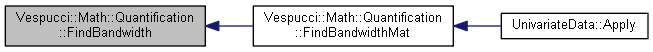
\includegraphics[width=350pt]{namespace_vespucci_1_1_math_1_1_quantification_a9ae95323be0190407aac32ec87605352_icgraph}
\end{center}
\end{figure}


\hypertarget{namespace_vespucci_1_1_math_1_1_quantification_a1f48a5ba0518572ef75a81985a267265}{\index{Vespucci\+::\+Math\+::\+Quantification@{Vespucci\+::\+Math\+::\+Quantification}!Find\+Bandwidth\+Mat@{Find\+Bandwidth\+Mat}}
\index{Find\+Bandwidth\+Mat@{Find\+Bandwidth\+Mat}!Vespucci\+::\+Math\+::\+Quantification@{Vespucci\+::\+Math\+::\+Quantification}}
\subsubsection[{Find\+Bandwidth\+Mat}]{\setlength{\rightskip}{0pt plus 5cm}arma\+::vec Vespucci\+::\+Math\+::\+Quantification\+::\+Find\+Bandwidth\+Mat (
\begin{DoxyParamCaption}
\item[{const arma\+::mat \&}]{X, }
\item[{arma\+::vec}]{abscissa, }
\item[{double \&}]{min, }
\item[{double \&}]{max, }
\item[{arma\+::mat \&}]{midlines, }
\item[{arma\+::mat \&}]{baselines, }
\item[{arma\+::uvec \&}]{boundaries}
\end{DoxyParamCaption}
)}}\label{namespace_vespucci_1_1_math_1_1_quantification_a1f48a5ba0518572ef75a81985a267265}


\hyperlink{namespace_vespucci_1_1_math_1_1_quantification_a1f48a5ba0518572ef75a81985a267265}{Vespucci\+::\+Math\+::\+Quantification\+::\+Find\+Bandwidth\+Mat}. 


\begin{DoxyParams}{Parameters}
{\em X} & \\
\hline
{\em abscissa} & \\
\hline
{\em min} & \\
\hline
{\em max} & \\
\hline
{\em midlines} & \\
\hline
{\em baselines} & \\
\hline
\end{DoxyParams}
\begin{DoxyReturn}{Returns}
Finds the bandwidth of every column of a arma\+::matrix. 
\end{DoxyReturn}


Definition at line 92 of file bandwidth.\+cpp.



Here is the call graph for this function\+:
\nopagebreak
\begin{figure}[H]
\begin{center}
\leavevmode
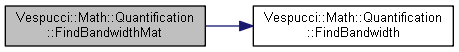
\includegraphics[width=350pt]{namespace_vespucci_1_1_math_1_1_quantification_a1f48a5ba0518572ef75a81985a267265_cgraph}
\end{center}
\end{figure}




Here is the caller graph for this function\+:
\nopagebreak
\begin{figure}[H]
\begin{center}
\leavevmode
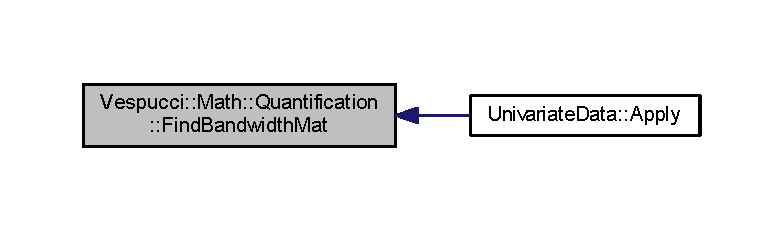
\includegraphics[width=350pt]{namespace_vespucci_1_1_math_1_1_quantification_a1f48a5ba0518572ef75a81985a267265_icgraph}
\end{center}
\end{figure}


\hypertarget{namespace_vespucci_1_1_math_1_1_quantification_a67d066d37ce165ac3e8c04d97436363c}{\index{Vespucci\+::\+Math\+::\+Quantification@{Vespucci\+::\+Math\+::\+Quantification}!Find\+Peak\+Max@{Find\+Peak\+Max}}
\index{Find\+Peak\+Max@{Find\+Peak\+Max}!Vespucci\+::\+Math\+::\+Quantification@{Vespucci\+::\+Math\+::\+Quantification}}
\subsubsection[{Find\+Peak\+Max}]{\setlength{\rightskip}{0pt plus 5cm}double Vespucci\+::\+Math\+::\+Quantification\+::\+Find\+Peak\+Max (
\begin{DoxyParamCaption}
\item[{const arma\+::vec \&}]{X, }
\item[{arma\+::uword}]{min\+\_\+index, }
\item[{arma\+::uword}]{max\+\_\+index, }
\item[{arma\+::uword \&}]{position}
\end{DoxyParamCaption}
)}}\label{namespace_vespucci_1_1_math_1_1_quantification_a67d066d37ce165ac3e8c04d97436363c}


\hyperlink{namespace_vespucci_1_1_math_1_1_quantification_a67d066d37ce165ac3e8c04d97436363c}{Vespucci\+::\+Math\+::\+Quantification\+::\+Find\+Peak\+Max}. 


\begin{DoxyParams}{Parameters}
{\em X} & \\
\hline
{\em min\+\_\+index} & \\
\hline
{\em max\+\_\+index} & \\
\hline
{\em position} & \\
\hline
\end{DoxyParams}
\begin{DoxyReturn}{Returns}
Finds the maximum of a peak bound by min\+\_\+index and max\+\_\+index 
\end{DoxyReturn}


Definition at line 31 of file maximum.\+cpp.



Here is the call graph for this function\+:
\nopagebreak
\begin{figure}[H]
\begin{center}
\leavevmode
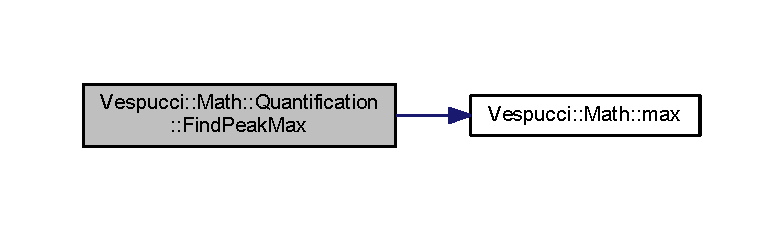
\includegraphics[width=350pt]{namespace_vespucci_1_1_math_1_1_quantification_a67d066d37ce165ac3e8c04d97436363c_cgraph}
\end{center}
\end{figure}




Here is the caller graph for this function\+:
\nopagebreak
\begin{figure}[H]
\begin{center}
\leavevmode
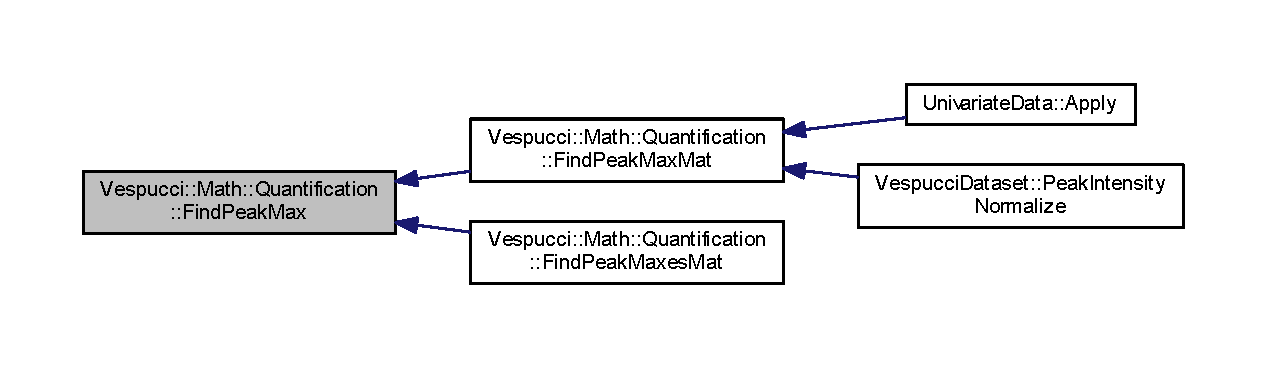
\includegraphics[width=350pt]{namespace_vespucci_1_1_math_1_1_quantification_a67d066d37ce165ac3e8c04d97436363c_icgraph}
\end{center}
\end{figure}


\hypertarget{namespace_vespucci_1_1_math_1_1_quantification_a6b4ad9737e416fb31ffc736465c3e87d}{\index{Vespucci\+::\+Math\+::\+Quantification@{Vespucci\+::\+Math\+::\+Quantification}!Find\+Peak\+Maxes\+Mat@{Find\+Peak\+Maxes\+Mat}}
\index{Find\+Peak\+Maxes\+Mat@{Find\+Peak\+Maxes\+Mat}!Vespucci\+::\+Math\+::\+Quantification@{Vespucci\+::\+Math\+::\+Quantification}}
\subsubsection[{Find\+Peak\+Maxes\+Mat}]{\setlength{\rightskip}{0pt plus 5cm}arma\+::mat Vespucci\+::\+Math\+::\+Quantification\+::\+Find\+Peak\+Maxes\+Mat (
\begin{DoxyParamCaption}
\item[{const arma\+::mat \&}]{X, }
\item[{arma\+::vec}]{abscissa, }
\item[{double \&}]{first\+\_\+min, }
\item[{double \&}]{first\+\_\+max, }
\item[{double \&}]{second\+\_\+min, }
\item[{double \&}]{second\+\_\+max, }
\item[{arma\+::mat}]{positions}
\end{DoxyParamCaption}
)}}\label{namespace_vespucci_1_1_math_1_1_quantification_a6b4ad9737e416fb31ffc736465c3e87d}


\hyperlink{namespace_vespucci_1_1_math_1_1_quantification_a6b4ad9737e416fb31ffc736465c3e87d}{Vespucci\+::\+Math\+::\+Quantification\+::\+Find\+Peak\+Maxes\+Mat}. 


\begin{DoxyParams}{Parameters}
{\em X} & \\
\hline
{\em abscissa} & \\
\hline
{\em first\+\_\+min} & \\
\hline
{\em first\+\_\+max} & \\
\hline
{\em second\+\_\+min} & \\
\hline
{\em second\+\_\+max} & \\
\hline
{\em positions} & \\
\hline
\end{DoxyParams}
\begin{DoxyReturn}{Returns}
Finds two peaks in the manner of Find\+Peak\+Max\+Mat 
\end{DoxyReturn}


Definition at line 84 of file maximum.\+cpp.



Here is the call graph for this function\+:
\nopagebreak
\begin{figure}[H]
\begin{center}
\leavevmode
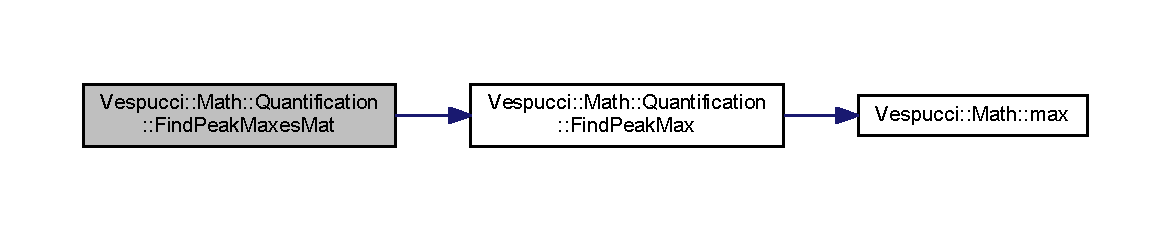
\includegraphics[width=350pt]{namespace_vespucci_1_1_math_1_1_quantification_a6b4ad9737e416fb31ffc736465c3e87d_cgraph}
\end{center}
\end{figure}


\hypertarget{namespace_vespucci_1_1_math_1_1_quantification_ac8a29afbde382eddd90a15749a8c3151}{\index{Vespucci\+::\+Math\+::\+Quantification@{Vespucci\+::\+Math\+::\+Quantification}!Find\+Peak\+Max\+Mat@{Find\+Peak\+Max\+Mat}}
\index{Find\+Peak\+Max\+Mat@{Find\+Peak\+Max\+Mat}!Vespucci\+::\+Math\+::\+Quantification@{Vespucci\+::\+Math\+::\+Quantification}}
\subsubsection[{Find\+Peak\+Max\+Mat}]{\setlength{\rightskip}{0pt plus 5cm}arma\+::vec Vespucci\+::\+Math\+::\+Quantification\+::\+Find\+Peak\+Max\+Mat (
\begin{DoxyParamCaption}
\item[{const arma\+::mat \&}]{X, }
\item[{arma\+::vec}]{abscissa, }
\item[{double \&}]{min, }
\item[{double \&}]{max, }
\item[{arma\+::vec \&}]{positions}
\end{DoxyParamCaption}
)}}\label{namespace_vespucci_1_1_math_1_1_quantification_ac8a29afbde382eddd90a15749a8c3151}


\hyperlink{namespace_vespucci_1_1_math_1_1_quantification_ac8a29afbde382eddd90a15749a8c3151}{Vespucci\+::\+Math\+::\+Quantification\+::\+Find\+Peak\+Max\+Mat}. 


\begin{DoxyParams}{Parameters}
{\em X} & \\
\hline
{\em abscissa} & \\
\hline
{\em min} & \\
\hline
{\em max} & \\
\hline
{\em positions} & \\
\hline
\end{DoxyParams}
\begin{DoxyReturn}{Returns}
Iterates Find\+Peak\+Mat over the columns of a arma\+::matrix. Finds the indices of specified min and max inputs 
\end{DoxyReturn}


Definition at line 50 of file maximum.\+cpp.



Here is the call graph for this function\+:
\nopagebreak
\begin{figure}[H]
\begin{center}
\leavevmode
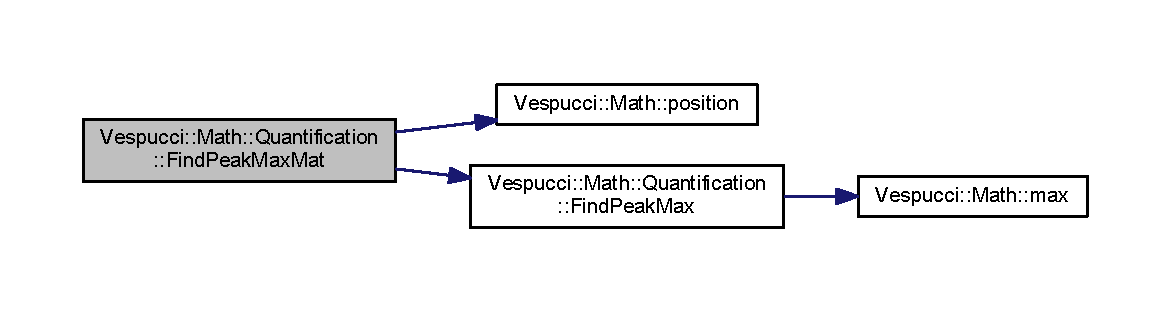
\includegraphics[width=350pt]{namespace_vespucci_1_1_math_1_1_quantification_ac8a29afbde382eddd90a15749a8c3151_cgraph}
\end{center}
\end{figure}




Here is the caller graph for this function\+:
\nopagebreak
\begin{figure}[H]
\begin{center}
\leavevmode
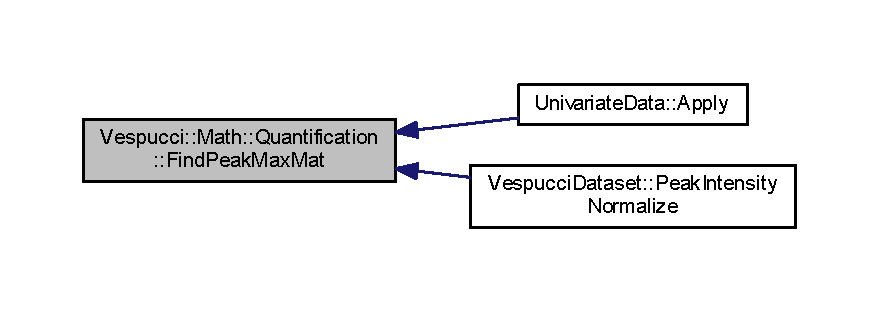
\includegraphics[width=350pt]{namespace_vespucci_1_1_math_1_1_quantification_ac8a29afbde382eddd90a15749a8c3151_icgraph}
\end{center}
\end{figure}


\hypertarget{namespace_vespucci_1_1_math_1_1_quantification_ad7bdec1b7cc7351cc6c4c5db0c28f069}{\index{Vespucci\+::\+Math\+::\+Quantification@{Vespucci\+::\+Math\+::\+Quantification}!Integrate\+Peak@{Integrate\+Peak}}
\index{Integrate\+Peak@{Integrate\+Peak}!Vespucci\+::\+Math\+::\+Quantification@{Vespucci\+::\+Math\+::\+Quantification}}
\subsubsection[{Integrate\+Peak}]{\setlength{\rightskip}{0pt plus 5cm}double Vespucci\+::\+Math\+::\+Quantification\+::\+Integrate\+Peak (
\begin{DoxyParamCaption}
\item[{const arma\+::vec \&}]{X, }
\item[{arma\+::uword}]{min\+\_\+index, }
\item[{arma\+::uword}]{max\+\_\+index, }
\item[{double}]{abscissa\+\_\+step, }
\item[{arma\+::vec \&}]{baseline}
\end{DoxyParamCaption}
)}}\label{namespace_vespucci_1_1_math_1_1_quantification_ad7bdec1b7cc7351cc6c4c5db0c28f069}


\hyperlink{namespace_vespucci_1_1_math_1_1_quantification_ad7bdec1b7cc7351cc6c4c5db0c28f069}{Vespucci\+::\+Math\+::\+Quantification\+::\+Integrate\+Peak}. 


\begin{DoxyParams}{Parameters}
{\em X} & \\
\hline
{\em min\+\_\+index} & \\
\hline
{\em max\+\_\+index} & \\
\hline
{\em abscissa\+\_\+step} & \\
\hline
{\em baseline} & \\
\hline
\end{DoxyParams}
\begin{DoxyReturn}{Returns}
Takes a Riemann sum under a peak defined by certain indices 
\end{DoxyReturn}


Definition at line 31 of file integration.\+cpp.



Here is the caller graph for this function\+:
\nopagebreak
\begin{figure}[H]
\begin{center}
\leavevmode
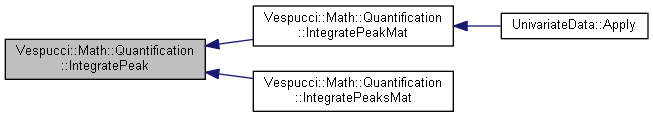
\includegraphics[width=350pt]{namespace_vespucci_1_1_math_1_1_quantification_ad7bdec1b7cc7351cc6c4c5db0c28f069_icgraph}
\end{center}
\end{figure}


\hypertarget{namespace_vespucci_1_1_math_1_1_quantification_a6bc1dd68cd6d9aa6c86d1b57c975f1aa}{\index{Vespucci\+::\+Math\+::\+Quantification@{Vespucci\+::\+Math\+::\+Quantification}!Integrate\+Peak\+Mat@{Integrate\+Peak\+Mat}}
\index{Integrate\+Peak\+Mat@{Integrate\+Peak\+Mat}!Vespucci\+::\+Math\+::\+Quantification@{Vespucci\+::\+Math\+::\+Quantification}}
\subsubsection[{Integrate\+Peak\+Mat}]{\setlength{\rightskip}{0pt plus 5cm}arma\+::vec Vespucci\+::\+Math\+::\+Quantification\+::\+Integrate\+Peak\+Mat (
\begin{DoxyParamCaption}
\item[{const arma\+::mat \&}]{X, }
\item[{arma\+::vec}]{abscissa, }
\item[{double \&}]{min, }
\item[{double \&}]{max, }
\item[{arma\+::mat \&}]{baselines, }
\item[{arma\+::uvec \&}]{boundaries}
\end{DoxyParamCaption}
)}}\label{namespace_vespucci_1_1_math_1_1_quantification_a6bc1dd68cd6d9aa6c86d1b57c975f1aa}


\hyperlink{namespace_vespucci_1_1_math_1_1_quantification_a6bc1dd68cd6d9aa6c86d1b57c975f1aa}{Vespucci\+::\+Math\+::\+Quantification\+::\+Integrate\+Peak\+Mat}. 


\begin{DoxyParams}{Parameters}
{\em X} & \\
\hline
{\em abscissa} & \\
\hline
{\em min} & \\
\hline
{\em max} & \\
\hline
{\em baselines} & \\
\hline
\end{DoxyParams}
\begin{DoxyReturn}{Returns}
Finds the index of specified start and end values, then calls Integrate\+Peak on each column of the arma\+::matrix 
\end{DoxyReturn}


Definition at line 56 of file integration.\+cpp.



Here is the call graph for this function\+:
\nopagebreak
\begin{figure}[H]
\begin{center}
\leavevmode
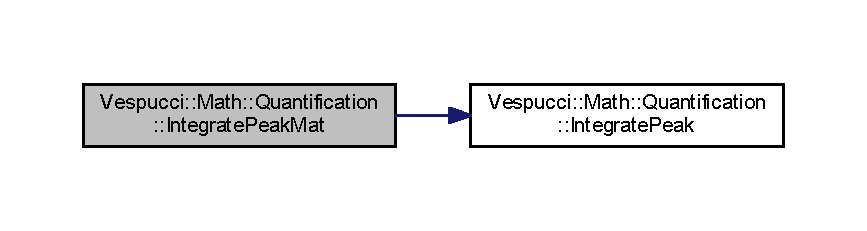
\includegraphics[width=350pt]{namespace_vespucci_1_1_math_1_1_quantification_a6bc1dd68cd6d9aa6c86d1b57c975f1aa_cgraph}
\end{center}
\end{figure}




Here is the caller graph for this function\+:
\nopagebreak
\begin{figure}[H]
\begin{center}
\leavevmode
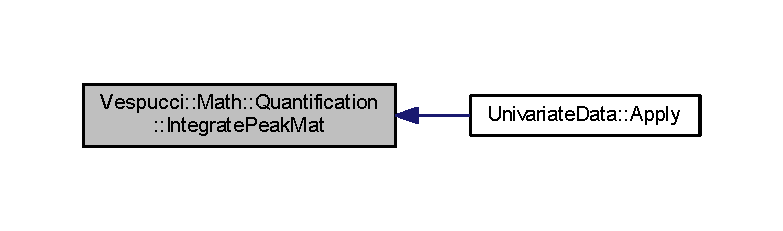
\includegraphics[width=350pt]{namespace_vespucci_1_1_math_1_1_quantification_a6bc1dd68cd6d9aa6c86d1b57c975f1aa_icgraph}
\end{center}
\end{figure}


\hypertarget{namespace_vespucci_1_1_math_1_1_quantification_a69e656fff0fae8013961de06b6ff72cc}{\index{Vespucci\+::\+Math\+::\+Quantification@{Vespucci\+::\+Math\+::\+Quantification}!Integrate\+Peaks\+Mat@{Integrate\+Peaks\+Mat}}
\index{Integrate\+Peaks\+Mat@{Integrate\+Peaks\+Mat}!Vespucci\+::\+Math\+::\+Quantification@{Vespucci\+::\+Math\+::\+Quantification}}
\subsubsection[{Integrate\+Peaks\+Mat}]{\setlength{\rightskip}{0pt plus 5cm}arma\+::mat Vespucci\+::\+Math\+::\+Quantification\+::\+Integrate\+Peaks\+Mat (
\begin{DoxyParamCaption}
\item[{const arma\+::mat \&}]{X, }
\item[{arma\+::vec}]{abscissa, }
\item[{double \&}]{first\+\_\+min, }
\item[{double \&}]{first\+\_\+max, }
\item[{double \&}]{second\+\_\+min, }
\item[{double \&}]{second\+\_\+max, }
\item[{arma\+::mat \&}]{first\+\_\+baselines, }
\item[{arma\+::mat \&}]{second\+\_\+baselines, }
\item[{arma\+::uvec \&}]{boundaries}
\end{DoxyParamCaption}
)}}\label{namespace_vespucci_1_1_math_1_1_quantification_a69e656fff0fae8013961de06b6ff72cc}


\hyperlink{namespace_vespucci_1_1_math_1_1_quantification_a69e656fff0fae8013961de06b6ff72cc}{Vespucci\+::\+Math\+::\+Quantification\+::\+Integrate\+Peaks\+Mat}. 


\begin{DoxyParams}{Parameters}
{\em X} & \\
\hline
{\em abscissa} & \\
\hline
{\em first\+\_\+min} & \\
\hline
{\em first\+\_\+max} & \\
\hline
{\em second\+\_\+min} & \\
\hline
{\em second\+\_\+max} & \\
\hline
{\em first\+\_\+baselines} & \\
\hline
{\em second\+\_\+baselines} & \\
\hline
\end{DoxyParams}
\begin{DoxyReturn}{Returns}
Performs two peak integrations 
\end{DoxyReturn}


Definition at line 90 of file integration.\+cpp.



Here is the call graph for this function\+:
\nopagebreak
\begin{figure}[H]
\begin{center}
\leavevmode
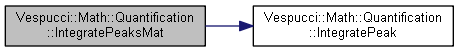
\includegraphics[width=350pt]{namespace_vespucci_1_1_math_1_1_quantification_a69e656fff0fae8013961de06b6ff72cc_cgraph}
\end{center}
\end{figure}



\chapter{Class Documentation}
\hypertarget{class_about_dialog}{}\section{About\+Dialog Class Reference}
\label{class_about_dialog}\index{About\+Dialog@{About\+Dialog}}


The \hyperlink{class_about_dialog}{About\+Dialog} class A Q\+Dialog that displays information about \hyperlink{namespace_vespucci}{Vespucci}.  




{\ttfamily \#include $<$aboutdialog.\+h$>$}

Inheritance diagram for About\+Dialog\+:\begin{figure}[H]
\begin{center}
\leavevmode
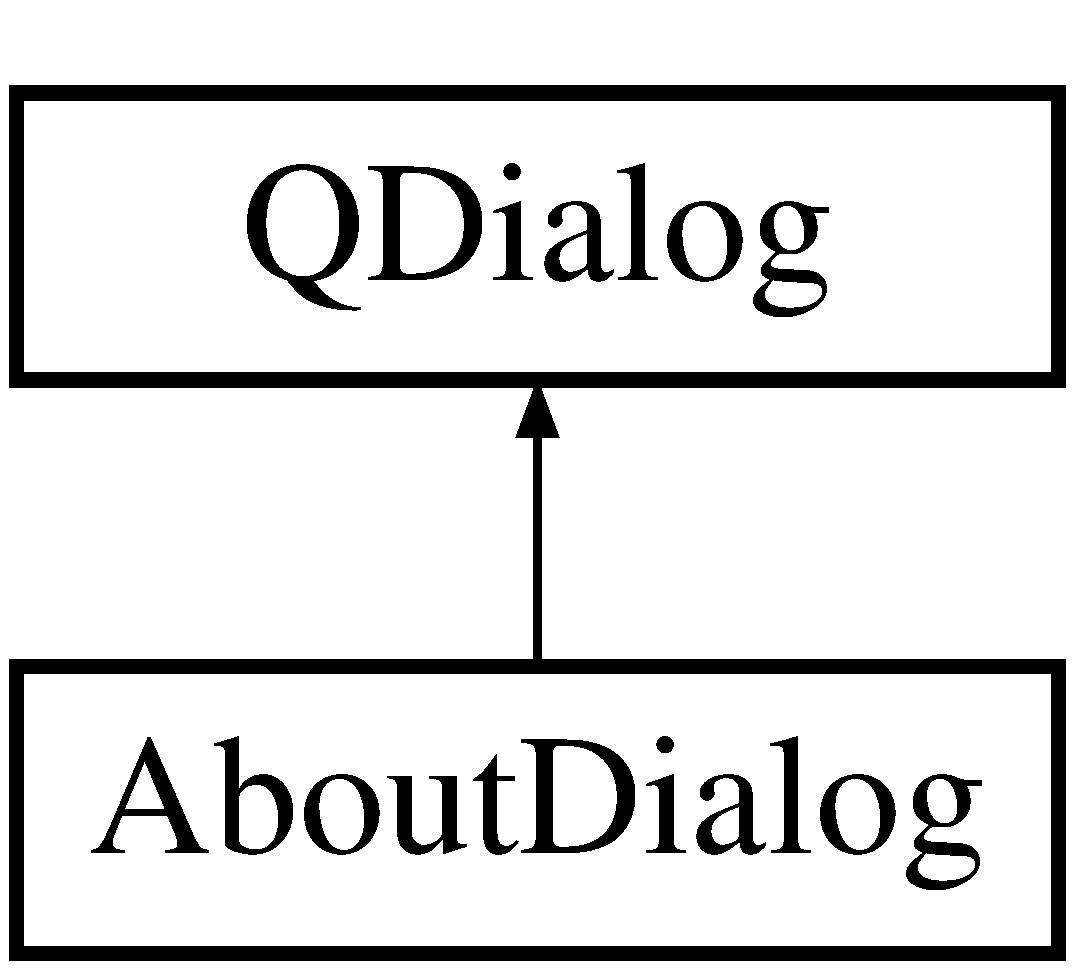
\includegraphics[height=2.000000cm]{class_about_dialog}
\end{center}
\end{figure}
\subsection*{Public Member Functions}
\begin{DoxyCompactItemize}
\item 
{\bfseries About\+Dialog} (Q\+Widget $\ast$parent=0)\hypertarget{class_about_dialog_ad96fc2ce8de7568ace543b7c69c71c56}{}\label{class_about_dialog_ad96fc2ce8de7568ace543b7c69c71c56}

\end{DoxyCompactItemize}


\subsection{Detailed Description}
The \hyperlink{class_about_dialog}{About\+Dialog} class A Q\+Dialog that displays information about \hyperlink{namespace_vespucci}{Vespucci}. 

Definition at line 31 of file aboutdialog.\+h.



The documentation for this class was generated from the following files\+:\begin{DoxyCompactItemize}
\item 
Vespucci/\+G\+U\+I/\+Display/aboutdialog.\+h\item 
Vespucci/\+G\+U\+I/\+Display/aboutdialog.\+cpp\end{DoxyCompactItemize}

\hypertarget{class_abscissa_interpolation_dialog}{}\section{Abscissa\+Interpolation\+Dialog Class Reference}
\label{class_abscissa_interpolation_dialog}\index{Abscissa\+Interpolation\+Dialog@{Abscissa\+Interpolation\+Dialog}}
Inheritance diagram for Abscissa\+Interpolation\+Dialog\+:\begin{figure}[H]
\begin{center}
\leavevmode
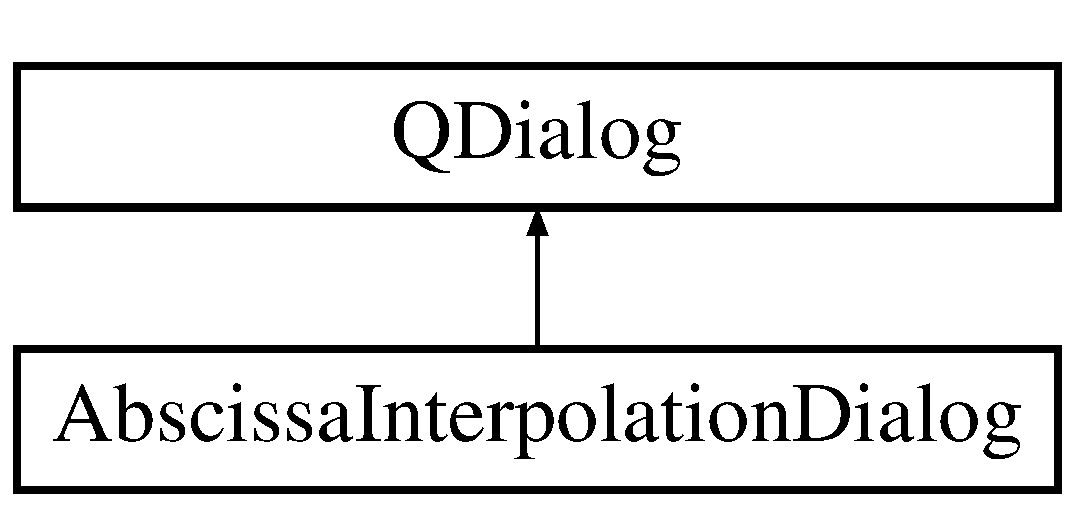
\includegraphics[height=2.000000cm]{class_abscissa_interpolation_dialog}
\end{center}
\end{figure}
\subsection*{Public Member Functions}
\begin{DoxyCompactItemize}
\item 
{\bfseries Abscissa\+Interpolation\+Dialog} (Q\+Widget $\ast$parent, \hyperlink{class_vespucci_workspace}{Vespucci\+Workspace} $\ast$ws, const Q\+String \&dataset\+\_\+key)\hypertarget{class_abscissa_interpolation_dialog_a6c5ad25cb8d3be8914bec8d9d820cf23}{}\label{class_abscissa_interpolation_dialog_a6c5ad25cb8d3be8914bec8d9d820cf23}

\end{DoxyCompactItemize}


\subsection{Detailed Description}


Definition at line 10 of file abscissainterpolationdialog.\+h.



The documentation for this class was generated from the following files\+:\begin{DoxyCompactItemize}
\item 
Vespucci/\+G\+U\+I/\+Processing/abscissainterpolationdialog.\+h\item 
Vespucci/\+G\+U\+I/\+Processing/abscissainterpolationdialog.\+cpp\end{DoxyCompactItemize}

\hypertarget{class_abscissa_transform_dialog}{}\section{Abscissa\+Transform\+Dialog Class Reference}
\label{class_abscissa_transform_dialog}\index{Abscissa\+Transform\+Dialog@{Abscissa\+Transform\+Dialog}}
Inheritance diagram for Abscissa\+Transform\+Dialog\+:\begin{figure}[H]
\begin{center}
\leavevmode
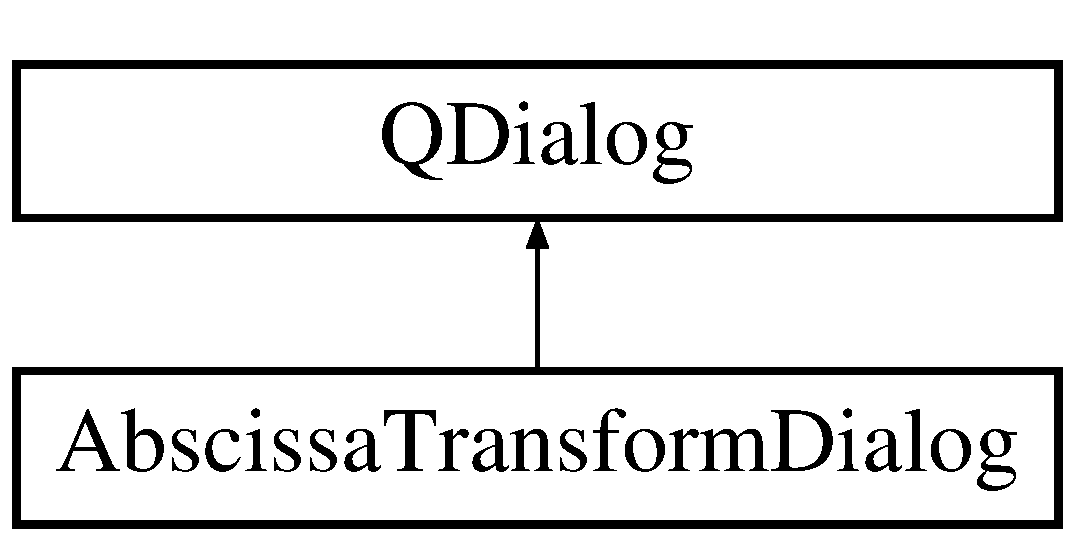
\includegraphics[height=2.000000cm]{class_abscissa_transform_dialog}
\end{center}
\end{figure}
\subsection*{Public Member Functions}
\begin{DoxyCompactItemize}
\item 
{\bfseries Abscissa\+Transform\+Dialog} (Q\+Widget $\ast$parent, \hyperlink{class_vespucci_workspace}{Vespucci\+Workspace} $\ast$ws, const Q\+String \&dataset\+\_\+key)\hypertarget{class_abscissa_transform_dialog_a20def5fdff77bc501e1afb57bccbd3d5}{}\label{class_abscissa_transform_dialog_a20def5fdff77bc501e1afb57bccbd3d5}

\end{DoxyCompactItemize}


\subsection{Detailed Description}


Definition at line 11 of file abscissatransformdialog.\+h.



The documentation for this class was generated from the following files\+:\begin{DoxyCompactItemize}
\item 
Vespucci/\+G\+U\+I/\+Processing/abscissatransformdialog.\+h\item 
Vespucci/\+G\+U\+I/\+Processing/abscissatransformdialog.\+cpp\end{DoxyCompactItemize}

\hypertarget{class_analysis_results}{\section{Analysis\+Results Class Reference}
\label{class_analysis_results}\index{Analysis\+Results@{Analysis\+Results}}
}


The \hyperlink{class_analysis_results}{Analysis\+Results} class A container for a mat object that allows a mat to be copied to a heap-\/allocated object (this) so pointers to that mat cannot go out of scope. These objects should be heap-\/allocated inside smart pointers.  




{\ttfamily \#include $<$analysisresults.\+h$>$}

\subsection*{Public Member Functions}
\begin{DoxyCompactItemize}
\item 
\hypertarget{class_analysis_results_a96290e00cecee6d9fea02ffb42633eeb}{{\bfseries Analysis\+Results} (mat value)}\label{class_analysis_results_a96290e00cecee6d9fea02ffb42633eeb}

\item 
\hypertarget{class_analysis_results_ae591750de59fc7c4a8bcb9d422cf161d}{mat {\bfseries value} ()}\label{class_analysis_results_ae591750de59fc7c4a8bcb9d422cf161d}

\item 
\hypertarget{class_analysis_results_a1ea6245771f569a72f0cccae21798270}{mat $\ast$ {\bfseries value\+\_\+ptr} ()}\label{class_analysis_results_a1ea6245771f569a72f0cccae21798270}

\end{DoxyCompactItemize}


\subsection{Detailed Description}
The \hyperlink{class_analysis_results}{Analysis\+Results} class A container for a mat object that allows a mat to be copied to a heap-\/allocated object (this) so pointers to that mat cannot go out of scope. These objects should be heap-\/allocated inside smart pointers. 

Definition at line 29 of file analysisresults.\+h.



The documentation for this class was generated from the following files\+:\begin{DoxyCompactItemize}
\item 
C\+:/\+Projects/\+Vespucci/develop/\+Data/\+Analysis/analysisresults.\+h\item 
C\+:/\+Projects/\+Vespucci/develop/\+Data/\+Analysis/analysisresults.\+cpp\end{DoxyCompactItemize}

\hypertarget{class_band_ratio_dialog}{\section{Band\+Ratio\+Dialog Class Reference}
\label{class_band_ratio_dialog}\index{Band\+Ratio\+Dialog@{Band\+Ratio\+Dialog}}
}


The \hyperlink{class_band_ratio_dialog}{Band\+Ratio\+Dialog} class The dialog that allows the user to create a band-\/ratio map.  




{\ttfamily \#include $<$bandratiodialog.\+h$>$}



Inheritance diagram for Band\+Ratio\+Dialog\+:\nopagebreak
\begin{figure}[H]
\begin{center}
\leavevmode
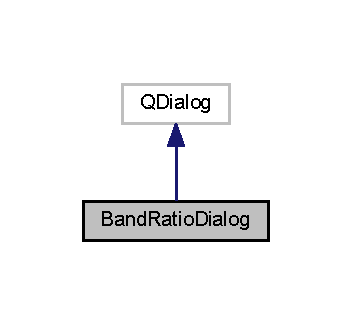
\includegraphics[width=169pt]{class_band_ratio_dialog__inherit__graph}
\end{center}
\end{figure}


Collaboration diagram for Band\+Ratio\+Dialog\+:\nopagebreak
\begin{figure}[H]
\begin{center}
\leavevmode
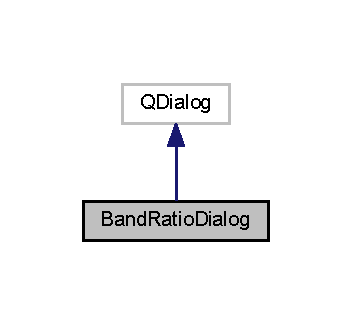
\includegraphics[width=169pt]{class_band_ratio_dialog__coll__graph}
\end{center}
\end{figure}
\subsection*{Public Member Functions}
\begin{DoxyCompactItemize}
\item 
\hypertarget{class_band_ratio_dialog_a9f8135f338936413f8a02e149e95df0a}{{\bfseries Band\+Ratio\+Dialog} (Q\+Widget $\ast$parent, \hyperlink{class_vespucci_workspace}{Vespucci\+Workspace} $\ast$ws, int row)}\label{class_band_ratio_dialog_a9f8135f338936413f8a02e149e95df0a}

\end{DoxyCompactItemize}


\subsection{Detailed Description}
The \hyperlink{class_band_ratio_dialog}{Band\+Ratio\+Dialog} class The dialog that allows the user to create a band-\/ratio map. 

Definition at line 34 of file bandratiodialog.\+h.



The documentation for this class was generated from the following files\+:\begin{DoxyCompactItemize}
\item 
C\+:/\+Projects/\+Vespucci/develop/\+G\+U\+I/\+Analysis/bandratiodialog.\+h\item 
C\+:/\+Projects/\+Vespucci/develop/\+G\+U\+I/\+Analysis/bandratiodialog.\+cpp\end{DoxyCompactItemize}

\hypertarget{class_baseline_dialog}{}\section{Baseline\+Dialog Class Reference}
\label{class_baseline_dialog}\index{Baseline\+Dialog@{Baseline\+Dialog}}


The \hyperlink{class_baseline_dialog}{Baseline\+Dialog} class The dialog that allows the user to baseline-\/correct the data.  




{\ttfamily \#include $<$baselinedialog.\+h$>$}

Inheritance diagram for Baseline\+Dialog\+:\begin{figure}[H]
\begin{center}
\leavevmode
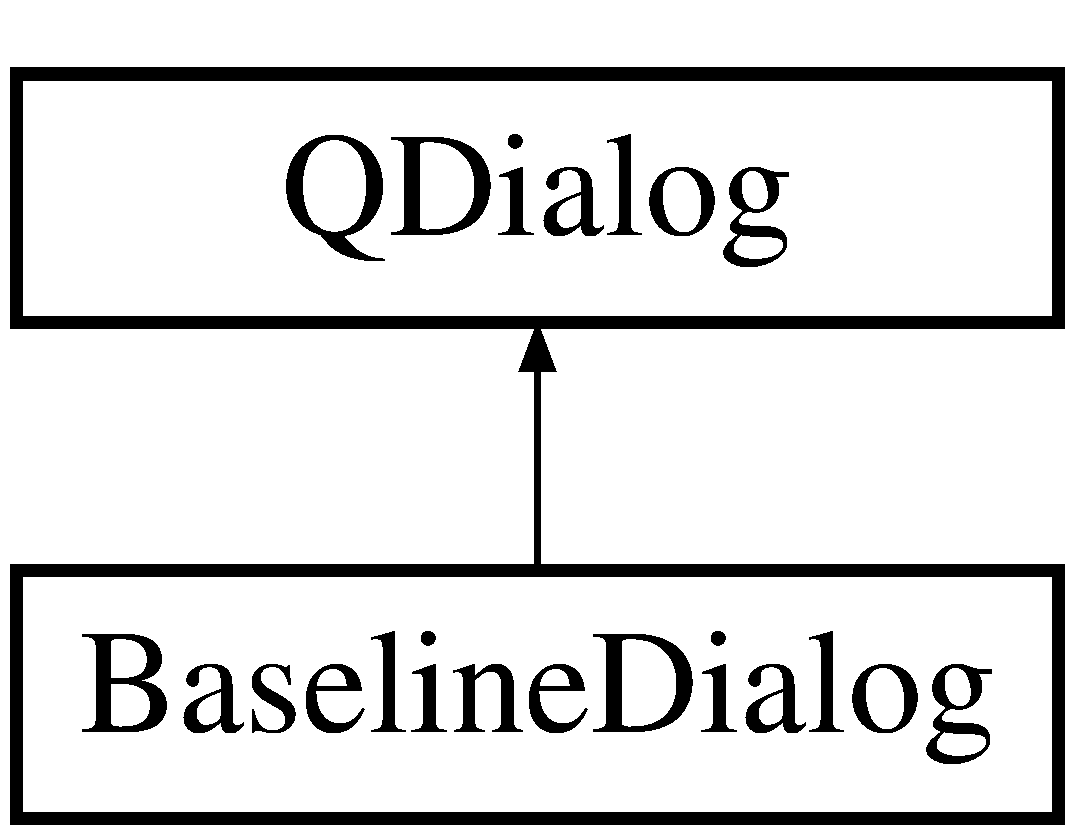
\includegraphics[height=2.000000cm]{class_baseline_dialog}
\end{center}
\end{figure}
\subsection*{Public Member Functions}
\begin{DoxyCompactItemize}
\item 
\hyperlink{class_baseline_dialog_ad7232611677ea102e9b81e9a0854774e}{Baseline\+Dialog} (Q\+Widget $\ast$parent, \hyperlink{class_vespucci_workspace}{Vespucci\+Workspace} $\ast$ws, const Q\+String \&dataset\+\_\+key)
\begin{DoxyCompactList}\small\item\em \hyperlink{class_baseline_dialog_ad7232611677ea102e9b81e9a0854774e}{Baseline\+Dialog\+::\+Baseline\+Dialog}. \end{DoxyCompactList}\end{DoxyCompactItemize}


\subsection{Detailed Description}
The \hyperlink{class_baseline_dialog}{Baseline\+Dialog} class The dialog that allows the user to baseline-\/correct the data. 

Definition at line 34 of file baselinedialog.\+h.



\subsection{Constructor \& Destructor Documentation}
\index{Baseline\+Dialog@{Baseline\+Dialog}!Baseline\+Dialog@{Baseline\+Dialog}}
\index{Baseline\+Dialog@{Baseline\+Dialog}!Baseline\+Dialog@{Baseline\+Dialog}}
\subsubsection[{\texorpdfstring{Baseline\+Dialog(\+Q\+Widget $\ast$parent, Vespucci\+Workspace $\ast$ws, const Q\+String \&dataset\+\_\+key)}{BaselineDialog(QWidget *parent, VespucciWorkspace *ws, const QString &dataset_key)}}]{\setlength{\rightskip}{0pt plus 5cm}Baseline\+Dialog\+::\+Baseline\+Dialog (
\begin{DoxyParamCaption}
\item[{Q\+Widget $\ast$}]{parent, }
\item[{{\bf Vespucci\+Workspace} $\ast$}]{ws, }
\item[{const Q\+String \&}]{dataset\+\_\+key}
\end{DoxyParamCaption}
)\hspace{0.3cm}{\ttfamily [explicit]}}\hypertarget{class_baseline_dialog_ad7232611677ea102e9b81e9a0854774e}{}\label{class_baseline_dialog_ad7232611677ea102e9b81e9a0854774e}


\hyperlink{class_baseline_dialog_ad7232611677ea102e9b81e9a0854774e}{Baseline\+Dialog\+::\+Baseline\+Dialog}. 


\begin{DoxyParams}{Parameters}
{\em parent} & Parent widget, required for Q\+Dialog \\
\hline
{\em ws} & The current workspace \\
\hline
{\em row} & The currently selected row in the dataset list widget \\
\hline
\end{DoxyParams}


Definition at line 29 of file baselinedialog.\+cpp.



The documentation for this class was generated from the following files\+:\begin{DoxyCompactItemize}
\item 
Vespucci/\+G\+U\+I/\+Processing/baselinedialog.\+h\item 
Vespucci/\+G\+U\+I/\+Processing/baselinedialog.\+cpp\end{DoxyCompactItemize}

\hypertarget{class_booleanize_dialog}{\section{Booleanize\+Dialog Class Reference}
\label{class_booleanize_dialog}\index{Booleanize\+Dialog@{Booleanize\+Dialog}}
}


Inheritance diagram for Booleanize\+Dialog\+:\nopagebreak
\begin{figure}[H]
\begin{center}
\leavevmode
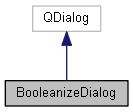
\includegraphics[width=172pt]{class_booleanize_dialog__inherit__graph}
\end{center}
\end{figure}


Collaboration diagram for Booleanize\+Dialog\+:\nopagebreak
\begin{figure}[H]
\begin{center}
\leavevmode
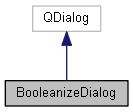
\includegraphics[width=172pt]{class_booleanize_dialog__coll__graph}
\end{center}
\end{figure}
\subsection*{Public Member Functions}
\begin{DoxyCompactItemize}
\item 
\hypertarget{class_booleanize_dialog_aae68d3541d225de9c90c8f5a128c7027}{{\bfseries Booleanize\+Dialog} (Q\+Widget $\ast$parent, \hyperlink{class_vespucci_workspace}{Vespucci\+Workspace} $\ast$ws, int row)}\label{class_booleanize_dialog_aae68d3541d225de9c90c8f5a128c7027}

\end{DoxyCompactItemize}


\subsection{Detailed Description}


Definition at line 12 of file booleanizedialog.\+h.



The documentation for this class was generated from the following files\+:\begin{DoxyCompactItemize}
\item 
C\+:/\+Projects/\+Vespucci/develop/\+G\+U\+I/\+Processing/booleanizedialog.\+h\item 
C\+:/\+Projects/\+Vespucci/develop/\+G\+U\+I/\+Processing/booleanizedialog.\+cpp\end{DoxyCompactItemize}

\hypertarget{class_bulk_conversion_dialog}{}\section{Bulk\+Conversion\+Dialog Class Reference}
\label{class_bulk_conversion_dialog}\index{Bulk\+Conversion\+Dialog@{Bulk\+Conversion\+Dialog}}
Inheritance diagram for Bulk\+Conversion\+Dialog\+:\begin{figure}[H]
\begin{center}
\leavevmode
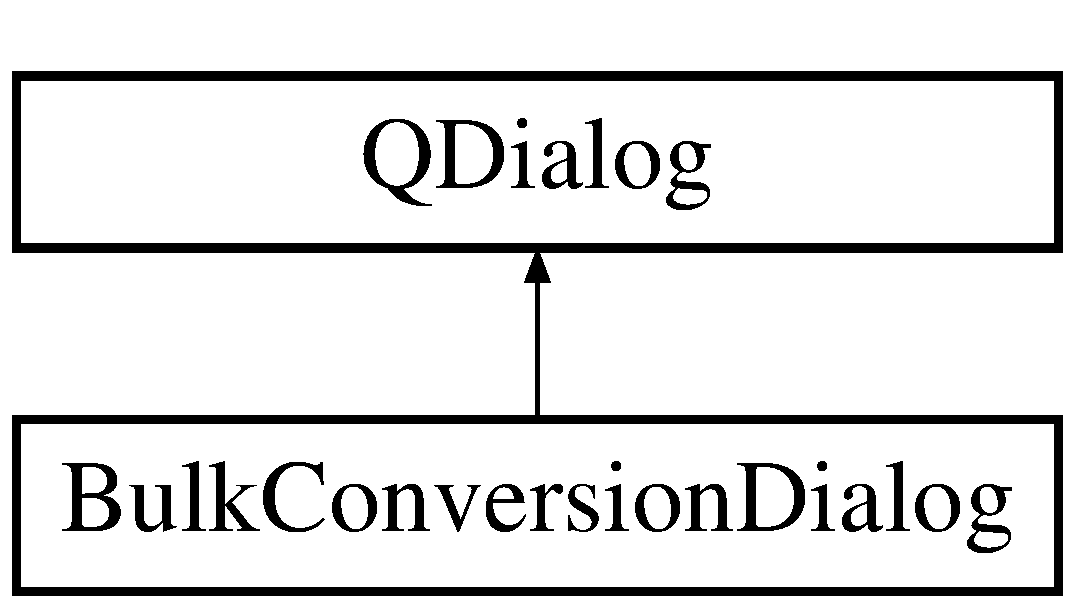
\includegraphics[height=2.000000cm]{class_bulk_conversion_dialog}
\end{center}
\end{figure}
\subsection*{Public Member Functions}
\begin{DoxyCompactItemize}
\item 
{\bfseries Bulk\+Conversion\+Dialog} (\hyperlink{class_main_window}{Main\+Window} $\ast$parent=0, \hyperlink{class_vespucci_workspace}{Vespucci\+Workspace} $\ast$ws=0)\hypertarget{class_bulk_conversion_dialog_ab7e3672dd71ab128e35f68cf9f155a89}{}\label{class_bulk_conversion_dialog_ab7e3672dd71ab128e35f68cf9f155a89}

\end{DoxyCompactItemize}


\subsection{Detailed Description}


Definition at line 14 of file bulkconversiondialog.\+h.



The documentation for this class was generated from the following files\+:\begin{DoxyCompactItemize}
\item 
Vespucci/\+G\+U\+I/\+Processing/bulkconversiondialog.\+h\item 
Vespucci/\+G\+U\+I/\+Processing/bulkconversiondialog.\+cpp\end{DoxyCompactItemize}

\hypertarget{struct_q_c_p_axis_painter_private_1_1_cached_label}{}\section{Q\+C\+P\+Axis\+Painter\+Private\+:\+:Cached\+Label Struct Reference}
\label{struct_q_c_p_axis_painter_private_1_1_cached_label}\index{Q\+C\+P\+Axis\+Painter\+Private\+::\+Cached\+Label@{Q\+C\+P\+Axis\+Painter\+Private\+::\+Cached\+Label}}
\subsection*{Public Attributes}
\begin{DoxyCompactItemize}
\item 
Q\+PointF {\bfseries offset}\hypertarget{struct_q_c_p_axis_painter_private_1_1_cached_label_a5f502db71c92e572f1e6f44f62c59d8e}{}\label{struct_q_c_p_axis_painter_private_1_1_cached_label_a5f502db71c92e572f1e6f44f62c59d8e}

\item 
Q\+Pixmap {\bfseries pixmap}\hypertarget{struct_q_c_p_axis_painter_private_1_1_cached_label_a461597cbd470914a9d24b64d16037a88}{}\label{struct_q_c_p_axis_painter_private_1_1_cached_label_a461597cbd470914a9d24b64d16037a88}

\end{DoxyCompactItemize}


\subsection{Detailed Description}


Definition at line 1367 of file qcustomplot.\+h.



The documentation for this struct was generated from the following file\+:\begin{DoxyCompactItemize}
\item 
Vespucci/\hyperlink{qcustomplot_8h}{qcustomplot.\+h}\end{DoxyCompactItemize}

\hypertarget{class_citation_dialog}{\section{Citation\+Dialog Class Reference}
\label{class_citation_dialog}\index{Citation\+Dialog@{Citation\+Dialog}}
}


The \hyperlink{class_citation_dialog}{Citation\+Dialog} class The dialog that displays how to cite \hyperlink{namespace_vespucci}{Vespucci}.  




{\ttfamily \#include $<$citationdialog.\+h$>$}



Inheritance diagram for Citation\+Dialog\+:\nopagebreak
\begin{figure}[H]
\begin{center}
\leavevmode
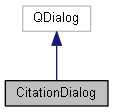
\includegraphics[width=157pt]{class_citation_dialog__inherit__graph}
\end{center}
\end{figure}


Collaboration diagram for Citation\+Dialog\+:\nopagebreak
\begin{figure}[H]
\begin{center}
\leavevmode
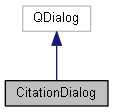
\includegraphics[width=157pt]{class_citation_dialog__coll__graph}
\end{center}
\end{figure}
\subsection*{Public Member Functions}
\begin{DoxyCompactItemize}
\item 
\hyperlink{class_citation_dialog_a566d6d063e20f68d619ff15412bda2f0}{Citation\+Dialog} (Q\+Widget $\ast$parent=0)
\begin{DoxyCompactList}\small\item\em \hyperlink{class_citation_dialog_a566d6d063e20f68d619ff15412bda2f0}{Citation\+Dialog\+::\+Citation\+Dialog}. \end{DoxyCompactList}\end{DoxyCompactItemize}


\subsection{Detailed Description}
The \hyperlink{class_citation_dialog}{Citation\+Dialog} class The dialog that displays how to cite \hyperlink{namespace_vespucci}{Vespucci}. 

Definition at line 32 of file citationdialog.\+h.



\subsection{Constructor \& Destructor Documentation}
\hypertarget{class_citation_dialog_a566d6d063e20f68d619ff15412bda2f0}{\index{Citation\+Dialog@{Citation\+Dialog}!Citation\+Dialog@{Citation\+Dialog}}
\index{Citation\+Dialog@{Citation\+Dialog}!Citation\+Dialog@{Citation\+Dialog}}
\subsubsection[{Citation\+Dialog}]{\setlength{\rightskip}{0pt plus 5cm}Citation\+Dialog\+::\+Citation\+Dialog (
\begin{DoxyParamCaption}
\item[{Q\+Widget $\ast$}]{parent = {\ttfamily 0}}
\end{DoxyParamCaption}
)\hspace{0.3cm}{\ttfamily [explicit]}}}\label{class_citation_dialog_a566d6d063e20f68d619ff15412bda2f0}


\hyperlink{class_citation_dialog_a566d6d063e20f68d619ff15412bda2f0}{Citation\+Dialog\+::\+Citation\+Dialog}. 


\begin{DoxyParams}{Parameters}
{\em parent} & Parent Q\+Widget, common for all Q\+Dialogs \\
\hline
\end{DoxyParams}


Definition at line 27 of file citationdialog.\+cpp.



The documentation for this class was generated from the following files\+:\begin{DoxyCompactItemize}
\item 
C\+:/\+Projects/\+Vespucci/develop/\+G\+U\+I/\+Display/citationdialog.\+h\item 
C\+:/\+Projects/\+Vespucci/develop/\+G\+U\+I/\+Display/citationdialog.\+cpp\end{DoxyCompactItemize}

\hypertarget{class_classical_least_squares_dialog}{}\section{Classical\+Least\+Squares\+Dialog Class Reference}
\label{class_classical_least_squares_dialog}\index{Classical\+Least\+Squares\+Dialog@{Classical\+Least\+Squares\+Dialog}}
Inheritance diagram for Classical\+Least\+Squares\+Dialog\+:\begin{figure}[H]
\begin{center}
\leavevmode
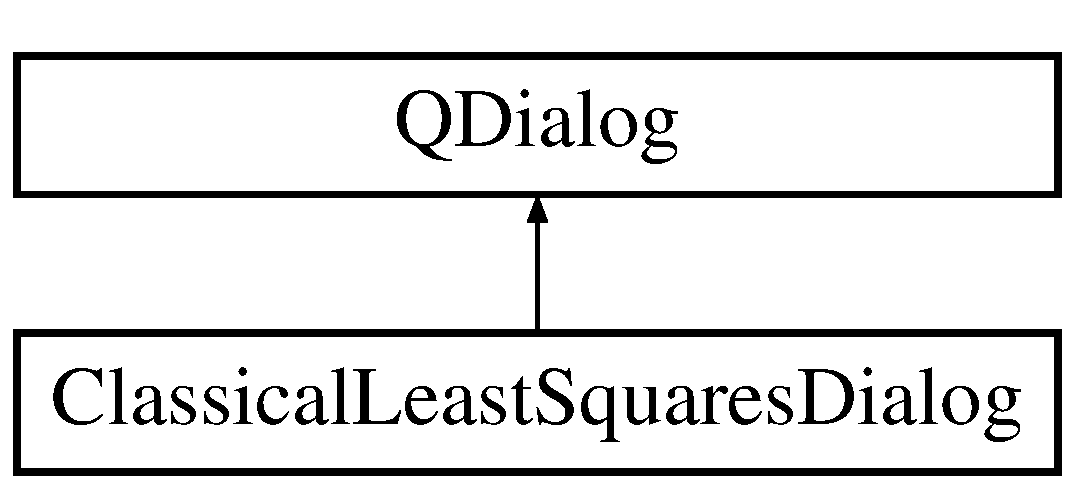
\includegraphics[height=2.000000cm]{class_classical_least_squares_dialog}
\end{center}
\end{figure}
\subsection*{Public Member Functions}
\begin{DoxyCompactItemize}
\item 
{\bfseries Classical\+Least\+Squares\+Dialog} (Q\+Widget $\ast$parent, \hyperlink{class_vespucci_workspace}{Vespucci\+Workspace} $\ast$ws, const Q\+String \&dataset\+\_\+key)\hypertarget{class_classical_least_squares_dialog_a1bf3e79a493d7924e4c9eec9b00d8763}{}\label{class_classical_least_squares_dialog_a1bf3e79a493d7924e4c9eec9b00d8763}

\end{DoxyCompactItemize}


\subsection{Detailed Description}


Definition at line 11 of file classicalleastsquaresdialog.\+h.



The documentation for this class was generated from the following files\+:\begin{DoxyCompactItemize}
\item 
Vespucci/\+G\+U\+I/\+Analysis/classicalleastsquaresdialog.\+h\item 
Vespucci/\+G\+U\+I/\+Analysis/classicalleastsquaresdialog.\+cpp\end{DoxyCompactItemize}

\hypertarget{class_crop_dialog}{}\section{Crop\+Dialog Class Reference}
\label{class_crop_dialog}\index{Crop\+Dialog@{Crop\+Dialog}}


The \hyperlink{class_crop_dialog}{Crop\+Dialog} class A dialog that allows the user to \char`\"{}\+Crop\char`\"{} the dataset (delete all spectra that are outside of a chosen spatial range).  




{\ttfamily \#include $<$cropdialog.\+h$>$}

Inheritance diagram for Crop\+Dialog\+:\begin{figure}[H]
\begin{center}
\leavevmode
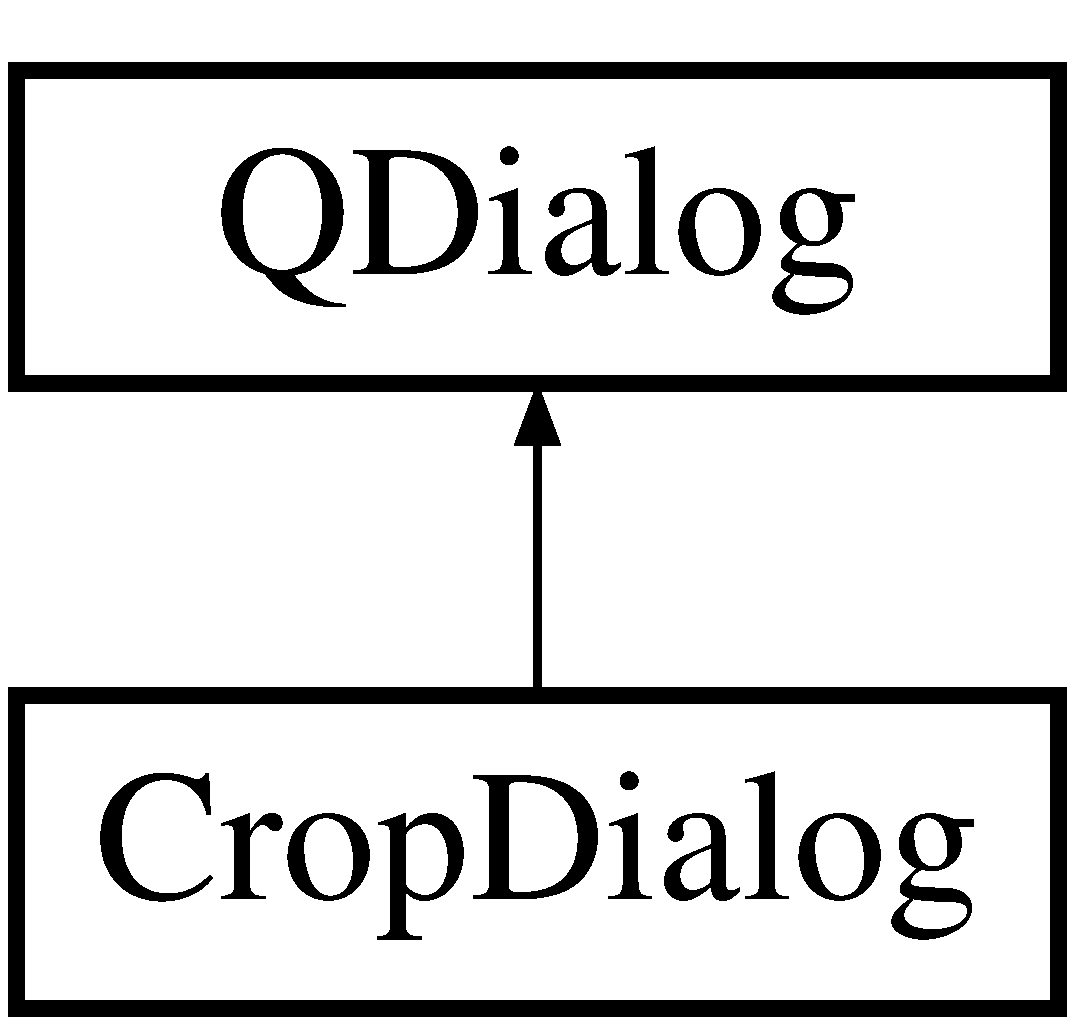
\includegraphics[height=2.000000cm]{class_crop_dialog}
\end{center}
\end{figure}
\subsection*{Public Member Functions}
\begin{DoxyCompactItemize}
\item 
\hyperlink{class_crop_dialog_a1a60341394d5a870a34d30d9626d3efc}{Crop\+Dialog} (Q\+Widget $\ast$parent, \hyperlink{class_vespucci_workspace}{Vespucci\+Workspace} $\ast$ws, const Q\+String \&dataset\+\_\+key)
\begin{DoxyCompactList}\small\item\em \hyperlink{class_crop_dialog_a1a60341394d5a870a34d30d9626d3efc}{Crop\+Dialog\+::\+Crop\+Dialog}. \end{DoxyCompactList}\end{DoxyCompactItemize}


\subsection{Detailed Description}
The \hyperlink{class_crop_dialog}{Crop\+Dialog} class A dialog that allows the user to \char`\"{}\+Crop\char`\"{} the dataset (delete all spectra that are outside of a chosen spatial range). 

Definition at line 35 of file cropdialog.\+h.



\subsection{Constructor \& Destructor Documentation}
\index{Crop\+Dialog@{Crop\+Dialog}!Crop\+Dialog@{Crop\+Dialog}}
\index{Crop\+Dialog@{Crop\+Dialog}!Crop\+Dialog@{Crop\+Dialog}}
\subsubsection[{\texorpdfstring{Crop\+Dialog(\+Q\+Widget $\ast$parent, Vespucci\+Workspace $\ast$ws, const Q\+String \&dataset\+\_\+key)}{CropDialog(QWidget *parent, VespucciWorkspace *ws, const QString &dataset_key)}}]{\setlength{\rightskip}{0pt plus 5cm}Crop\+Dialog\+::\+Crop\+Dialog (
\begin{DoxyParamCaption}
\item[{Q\+Widget $\ast$}]{parent, }
\item[{{\bf Vespucci\+Workspace} $\ast$}]{ws, }
\item[{const Q\+String \&}]{dataset\+\_\+key}
\end{DoxyParamCaption}
)\hspace{0.3cm}{\ttfamily [explicit]}}\hypertarget{class_crop_dialog_a1a60341394d5a870a34d30d9626d3efc}{}\label{class_crop_dialog_a1a60341394d5a870a34d30d9626d3efc}


\hyperlink{class_crop_dialog_a1a60341394d5a870a34d30d9626d3efc}{Crop\+Dialog\+::\+Crop\+Dialog}. 


\begin{DoxyParams}{Parameters}
{\em parent} & Parent Q\+Widget \\
\hline
{\em ws} & The current workspace \\
\hline
{\em row} & Currently selected row \\
\hline
\end{DoxyParams}


Definition at line 31 of file cropdialog.\+cpp.



The documentation for this class was generated from the following files\+:\begin{DoxyCompactItemize}
\item 
Vespucci/\+G\+U\+I/\+Processing/cropdialog.\+h\item 
Vespucci/\+G\+U\+I/\+Processing/cropdialog.\+cpp\end{DoxyCompactItemize}

\hypertarget{class_vespucci_1_1_external_1_1data__object}{}\section{Vespucci\+:\+:External\+:\+:data\+\_\+object Class Reference}
\label{class_vespucci_1_1_external_1_1data__object}\index{Vespucci\+::\+External\+::data\+\_\+object@{Vespucci\+::\+External\+::data\+\_\+object}}
\subsection*{Public Member Functions}
\begin{DoxyCompactItemize}
\item 
{\bfseries data\+\_\+object} (const char $\ast$name, int n\+\_\+rows, int n\+\_\+cols, const void\+\_\+allocator \&void\+\_\+alloc)\hypertarget{class_vespucci_1_1_external_1_1data__object_a028e2ac605bdccad7171e3ca3a8b61f1}{}\label{class_vespucci_1_1_external_1_1data__object_a028e2ac605bdccad7171e3ca3a8b61f1}

\item 
void {\bfseries push\+\_\+back} (double val)\hypertarget{class_vespucci_1_1_external_1_1data__object_ae1d797ae9b976c0fa54221b308629851}{}\label{class_vespucci_1_1_external_1_1data__object_ae1d797ae9b976c0fa54221b308629851}

\end{DoxyCompactItemize}


\subsection{Detailed Description}


Definition at line 21 of file interprocesssender.\+h.



The documentation for this class was generated from the following file\+:\begin{DoxyCompactItemize}
\item 
Vespucci/\+External/interprocesssender.\+h\end{DoxyCompactItemize}

\hypertarget{class_data_extractor_dialog}{\section{Data\+Extractor\+Dialog Class Reference}
\label{class_data_extractor_dialog}\index{Data\+Extractor\+Dialog@{Data\+Extractor\+Dialog}}
}


The \hyperlink{class_data_extractor_dialog}{Data\+Extractor\+Dialog} class A dialog that allows the user to create a new dataset from a map, based on map values.  




{\ttfamily \#include $<$dataextractordialog.\+h$>$}



Inheritance diagram for Data\+Extractor\+Dialog\+:\nopagebreak
\begin{figure}[H]
\begin{center}
\leavevmode
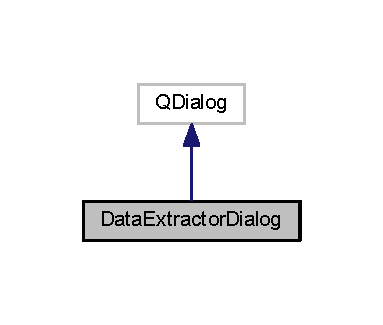
\includegraphics[width=184pt]{class_data_extractor_dialog__inherit__graph}
\end{center}
\end{figure}


Collaboration diagram for Data\+Extractor\+Dialog\+:\nopagebreak
\begin{figure}[H]
\begin{center}
\leavevmode
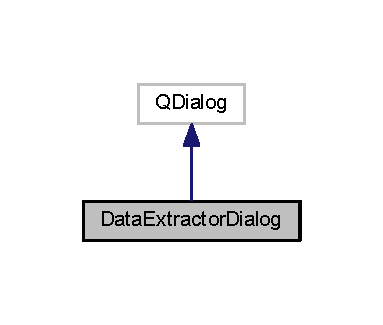
\includegraphics[width=184pt]{class_data_extractor_dialog__coll__graph}
\end{center}
\end{figure}
\subsection*{Public Member Functions}
\begin{DoxyCompactItemize}
\item 
\hyperlink{class_data_extractor_dialog_a1f258b0b0a524e2a2b574fe170ed7fdb}{Data\+Extractor\+Dialog} (Q\+Widget $\ast$parent, \hyperlink{class_map_data}{Map\+Data} $\ast$map, Q\+Shared\+Pointer$<$ \hyperlink{class_vespucci_dataset}{Vespucci\+Dataset} $>$ dataset, \hyperlink{class_main_window}{Main\+Window} $\ast$main\+\_\+window)
\begin{DoxyCompactList}\small\item\em \hyperlink{class_data_extractor_dialog_a1f258b0b0a524e2a2b574fe170ed7fdb}{Data\+Extractor\+Dialog\+::\+Data\+Extractor\+Dialog}. \end{DoxyCompactList}\item 
\hypertarget{class_data_extractor_dialog_a535646a4cce7c7e2e3b45589f0ee54aa}{{\bfseries Data\+Extractor\+Dialog} (Q\+Widget $\ast$parent, vec data, Q\+Shared\+Pointer$<$ \hyperlink{class_vespucci_dataset}{Vespucci\+Dataset} $>$ dataset, \hyperlink{class_main_window}{Main\+Window} $\ast$main\+\_\+window, Q\+String name)}\label{class_data_extractor_dialog_a535646a4cce7c7e2e3b45589f0ee54aa}

\end{DoxyCompactItemize}


\subsection{Detailed Description}
The \hyperlink{class_data_extractor_dialog}{Data\+Extractor\+Dialog} class A dialog that allows the user to create a new dataset from a map, based on map values. 

Definition at line 37 of file dataextractordialog.\+h.



\subsection{Constructor \& Destructor Documentation}
\hypertarget{class_data_extractor_dialog_a1f258b0b0a524e2a2b574fe170ed7fdb}{\index{Data\+Extractor\+Dialog@{Data\+Extractor\+Dialog}!Data\+Extractor\+Dialog@{Data\+Extractor\+Dialog}}
\index{Data\+Extractor\+Dialog@{Data\+Extractor\+Dialog}!Data\+Extractor\+Dialog@{Data\+Extractor\+Dialog}}
\subsubsection[{Data\+Extractor\+Dialog}]{\setlength{\rightskip}{0pt plus 5cm}Data\+Extractor\+Dialog\+::\+Data\+Extractor\+Dialog (
\begin{DoxyParamCaption}
\item[{Q\+Widget $\ast$}]{parent, }
\item[{{\bf Map\+Data} $\ast$}]{map, }
\item[{Q\+Shared\+Pointer$<$ {\bf Vespucci\+Dataset} $>$}]{dataset, }
\item[{{\bf Main\+Window} $\ast$}]{main\+\_\+window}
\end{DoxyParamCaption}
)}}\label{class_data_extractor_dialog_a1f258b0b0a524e2a2b574fe170ed7fdb}


\hyperlink{class_data_extractor_dialog_a1f258b0b0a524e2a2b574fe170ed7fdb}{Data\+Extractor\+Dialog\+::\+Data\+Extractor\+Dialog}. 


\begin{DoxyParams}{Parameters}
{\em parent} & Parent Q\+Widget \\
\hline
{\em map} & The map from which the new dataset is created \\
\hline
{\em dataset} & The current dataset from which the new dataset is created \\
\hline
{\em main\+\_\+window} & The main window of the program. \\
\hline
\end{DoxyParams}


Definition at line 31 of file dataextractordialog.\+cpp.



Here is the call graph for this function\+:\nopagebreak
\begin{figure}[H]
\begin{center}
\leavevmode
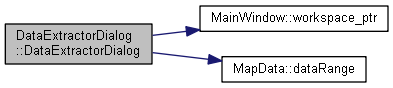
\includegraphics[width=350pt]{class_data_extractor_dialog_a1f258b0b0a524e2a2b574fe170ed7fdb_cgraph}
\end{center}
\end{figure}




The documentation for this class was generated from the following files\+:\begin{DoxyCompactItemize}
\item 
C\+:/\+Projects/\+Vespucci/develop/\+G\+U\+I/\+Processing/dataextractordialog.\+h\item 
C\+:/\+Projects/\+Vespucci/develop/\+G\+U\+I/\+Processing/dataextractordialog.\+cpp\end{DoxyCompactItemize}

\hypertarget{class_data_model}{}\section{Data\+Model Class Reference}
\label{class_data_model}\index{Data\+Model@{Data\+Model}}
\subsection*{Public Member Functions}
\begin{DoxyCompactItemize}
\item 
Q\+Shared\+Pointer$<$ \hyperlink{class_vespucci_dataset}{Vespucci\+Dataset} $>$ \hyperlink{class_data_model_a39a26795ff351c8f25144c022761c601}{Get\+Dataset} (const Q\+String \&key) const 
\begin{DoxyCompactList}\small\item\em \hyperlink{class_data_model_a39a26795ff351c8f25144c022761c601}{Data\+Model\+::\+Get\+Dataset} Get the \hyperlink{class_vespucci_dataset}{Vespucci\+Dataset} named key. \end{DoxyCompactList}\item 
Q\+Shared\+Pointer$<$ \hyperlink{class_analysis_results}{Analysis\+Results} $>$ \hyperlink{class_data_model_af277d915c6a3aa8a2d3d38378bfdd02f}{Get\+Results} (const Q\+String \&dataset\+\_\+key, const Q\+String \&results\+\_\+key) const 
\begin{DoxyCompactList}\small\item\em \hyperlink{class_data_model_af277d915c6a3aa8a2d3d38378bfdd02f}{Data\+Model\+::\+Get\+Results} Get the \hyperlink{class_analysis_results}{Analysis\+Results} object named results\+\_\+key from the dataset named dataset\+\_\+key. \end{DoxyCompactList}\item 
Q\+Shared\+Pointer$<$ \hyperlink{class_analysis_results}{Analysis\+Results} $>$ {\bfseries Get\+Results} (const Q\+String\+List \&keys) const \hypertarget{class_data_model_a176e3a30663cedcdfeb8ff43e96c3f08}{}\label{class_data_model_a176e3a30663cedcdfeb8ff43e96c3f08}

\item 
Q\+Shared\+Pointer$<$ \hyperlink{class_map_data}{Map\+Data} $>$ \hyperlink{class_data_model_a190e371dfaa3045527af6f6d2e41cf32}{Get\+Map} (const Q\+String \&dataset\+\_\+key, const Q\+String \&map\+\_\+key) const 
\begin{DoxyCompactList}\small\item\em \hyperlink{class_data_model_a190e371dfaa3045527af6f6d2e41cf32}{Data\+Model\+::\+Get\+Map} Get the \hyperlink{class_map_data}{Map\+Data} object named map\+\_\+key from dataset named dataset\+\_\+key. \end{DoxyCompactList}\item 
Q\+Shared\+Pointer$<$ \hyperlink{class_map_data}{Map\+Data} $>$ {\bfseries Get\+Map} (const Q\+String\+List \&keys) const \hypertarget{class_data_model_aad98e14defecb0477347a5fd36d8f6a2}{}\label{class_data_model_aad98e14defecb0477347a5fd36d8f6a2}

\item 
const mat \& {\bfseries Get\+Results\+Matrix} (const Q\+String \&dataset\+\_\+key, const Q\+String \&results\+\_\+key, const Q\+String \&matrix\+\_\+key) const \hypertarget{class_data_model_af2b05c5c8baaaba3c527c93da653ce09}{}\label{class_data_model_af2b05c5c8baaaba3c527c93da653ce09}

\item 
const mat \& {\bfseries Get\+Results\+Matrix} (const Q\+String\+List \&keys) const \hypertarget{class_data_model_a3198834d9eae938358dae1b0a51dd97d}{}\label{class_data_model_a3198834d9eae938358dae1b0a51dd97d}

\item 
const mat \& \hyperlink{class_data_model_ad168adfafdd3c9c6a7317a77df2c62e5}{Get\+Core\+Matrix} (const Q\+String \&dataset\+\_\+key, const Q\+String \&matrix\+\_\+key) const 
\begin{DoxyCompactList}\small\item\em \hyperlink{class_data_model_ad168adfafdd3c9c6a7317a77df2c62e5}{Data\+Model\+::\+Get\+Core\+Matrix}. \end{DoxyCompactList}\item 
const mat \& {\bfseries Get\+Core\+Matrix} (const Q\+String\+List \&keys) const \hypertarget{class_data_model_a8ef59d0778dc0c9605c46312291c25bb}{}\label{class_data_model_a8ef59d0778dc0c9605c46312291c25bb}

\item 
const mat \& \hyperlink{class_data_model_a826f3ec440b4fbcecb47eb9f1e7ceb3f}{Get\+Auxiliary\+Matrix} (const Q\+String \&dataset\+\_\+key, const Q\+String \&matrix\+\_\+key) const 
\begin{DoxyCompactList}\small\item\em \hyperlink{class_data_model_a826f3ec440b4fbcecb47eb9f1e7ceb3f}{Data\+Model\+::\+Get\+Auxiliary\+Matrix}. \end{DoxyCompactList}\item 
const mat \& {\bfseries Get\+Auxiliary\+Matrix} (const Q\+String\+List \&keys) const \hypertarget{class_data_model_a2426bc75ca0cf413fcbebb63bee0a326}{}\label{class_data_model_a2426bc75ca0cf413fcbebb63bee0a326}

\item 
const mat \& {\bfseries Get\+Matrix} (const Q\+String \&dataset\+\_\+key, const Q\+String \&matrix\+\_\+key) const \hypertarget{class_data_model_a2752763eb2c2d7be9cb10b45024ad8d6}{}\label{class_data_model_a2752763eb2c2d7be9cb10b45024ad8d6}

\item 
const mat \& {\bfseries Get\+Matrix} (const Q\+String\+List \&keys) const \hypertarget{class_data_model_a249dcd7395fc083902f5a0df3d0ed11c}{}\label{class_data_model_a249dcd7395fc083902f5a0df3d0ed11c}

\item 
bool {\bfseries Mappable} (const Q\+String\+List \&keys) const \hypertarget{class_data_model_a84b028bda5d4bf5719769164b32bdfc8}{}\label{class_data_model_a84b028bda5d4bf5719769164b32bdfc8}

\item 
bool {\bfseries Plottable} (const Q\+String\+List \&keys) const \hypertarget{class_data_model_ab41d55c9e713496d8f1eaecb8d37f546}{}\label{class_data_model_ab41d55c9e713496d8f1eaecb8d37f546}

\item 
Q\+String\+List \hyperlink{class_data_model_ae8e2a93a6c71ca636957faa8208eb6cc}{Dataset\+Names} () const 
\begin{DoxyCompactList}\small\item\em \hyperlink{class_data_model_ae8e2a93a6c71ca636957faa8208eb6cc}{Data\+Model\+::\+Dataset\+Names}. \end{DoxyCompactList}\item 
Q\+String\+List \hyperlink{class_data_model_a70071e275893667961ff4262f8d28c9e}{Analysis\+Results\+Names} (const Q\+String \&dataset\+\_\+key) const 
\begin{DoxyCompactList}\small\item\em \hyperlink{class_data_model_a70071e275893667961ff4262f8d28c9e}{Data\+Model\+::\+Analysis\+Results\+Names}. \end{DoxyCompactList}\item 
Q\+String\+List \hyperlink{class_data_model_a4086ff5d73459e7499f6f939e0ab3684}{Auxiliary\+Matrix\+Names} (const Q\+String \&dataset\+\_\+key) const 
\begin{DoxyCompactList}\small\item\em \hyperlink{class_data_model_a4086ff5d73459e7499f6f939e0ab3684}{Data\+Model\+::\+Auxiliary\+Matrix\+Names}. \end{DoxyCompactList}\item 
Q\+String\+List {\bfseries Core\+Matrix\+Names} (const Q\+String \&dataset\+\_\+key)\hypertarget{class_data_model_a92c4ff18028cdac1ee4f82fa96a571ca}{}\label{class_data_model_a92c4ff18028cdac1ee4f82fa96a571ca}

\item 
void \hyperlink{class_data_model_a59701ea222dc2cd8cdfb9d53cd2dcc72}{Add\+Dataset} (Q\+Shared\+Pointer$<$ \hyperlink{class_vespucci_dataset}{Vespucci\+Dataset} $>$ dataset)
\begin{DoxyCompactList}\small\item\em \hyperlink{class_data_model_a59701ea222dc2cd8cdfb9d53cd2dcc72}{Data\+Model\+::\+Add\+Dataset}. \end{DoxyCompactList}\item 
void \hyperlink{class_data_model_af0974f3a7271801470c3b5d7c7090eaf}{Remove\+Dataset} (const Q\+String \&name)
\begin{DoxyCompactList}\small\item\em \hyperlink{class_data_model_af0974f3a7271801470c3b5d7c7090eaf}{Data\+Model\+::\+Remove\+Dataset}. \end{DoxyCompactList}\item 
const mat \& {\bfseries Empty\+Matrix} () const \hypertarget{class_data_model_a699c4261005d596c4ce4b7132020c3a8}{}\label{class_data_model_a699c4261005d596c4ce4b7132020c3a8}

\item 
bool {\bfseries Has\+Dataset} (const Q\+String \&key) const \hypertarget{class_data_model_a0a3152f311a09d9011a6d00e85a2e8ac}{}\label{class_data_model_a0a3152f311a09d9011a6d00e85a2e8ac}

\end{DoxyCompactItemize}


\subsection{Detailed Description}


Definition at line 24 of file datamodel.\+h.



\subsection{Member Function Documentation}
\index{Data\+Model@{Data\+Model}!Add\+Dataset@{Add\+Dataset}}
\index{Add\+Dataset@{Add\+Dataset}!Data\+Model@{Data\+Model}}
\subsubsection[{\texorpdfstring{Add\+Dataset(\+Q\+Shared\+Pointer$<$ Vespucci\+Dataset $>$ dataset)}{AddDataset(QSharedPointer< VespucciDataset > dataset)}}]{\setlength{\rightskip}{0pt plus 5cm}void Data\+Model\+::\+Add\+Dataset (
\begin{DoxyParamCaption}
\item[{Q\+Shared\+Pointer$<$ {\bf Vespucci\+Dataset} $>$}]{dataset}
\end{DoxyParamCaption}
)}\hypertarget{class_data_model_a59701ea222dc2cd8cdfb9d53cd2dcc72}{}\label{class_data_model_a59701ea222dc2cd8cdfb9d53cd2dcc72}


\hyperlink{class_data_model_a59701ea222dc2cd8cdfb9d53cd2dcc72}{Data\+Model\+::\+Add\+Dataset}. 


\begin{DoxyParams}{Parameters}
{\em dataset} & Refuses to add a dataset if a dataset with that name already exists will throw invalid\+\_\+argument. \hyperlink{class_vespucci_workspace}{Vespucci\+Workspace} should handle it. \\
\hline
\end{DoxyParams}


Definition at line 301 of file datamodel.\+cpp.

\index{Data\+Model@{Data\+Model}!Analysis\+Results\+Names@{Analysis\+Results\+Names}}
\index{Analysis\+Results\+Names@{Analysis\+Results\+Names}!Data\+Model@{Data\+Model}}
\subsubsection[{\texorpdfstring{Analysis\+Results\+Names(const Q\+String \&dataset\+\_\+key) const }{AnalysisResultsNames(const QString &dataset_key) const }}]{\setlength{\rightskip}{0pt plus 5cm}Q\+String\+List Data\+Model\+::\+Analysis\+Results\+Names (
\begin{DoxyParamCaption}
\item[{const Q\+String \&}]{dataset\+\_\+key}
\end{DoxyParamCaption}
) const}\hypertarget{class_data_model_a70071e275893667961ff4262f8d28c9e}{}\label{class_data_model_a70071e275893667961ff4262f8d28c9e}


\hyperlink{class_data_model_a70071e275893667961ff4262f8d28c9e}{Data\+Model\+::\+Analysis\+Results\+Names}. 


\begin{DoxyParams}{Parameters}
{\em dataset\+\_\+key} & \\
\hline
\end{DoxyParams}
\begin{DoxyReturn}{Returns}
Throws invalid\+\_\+argument if dataset doesn\textquotesingle{}t exist 
\end{DoxyReturn}


Definition at line 260 of file datamodel.\+cpp.

\index{Data\+Model@{Data\+Model}!Auxiliary\+Matrix\+Names@{Auxiliary\+Matrix\+Names}}
\index{Auxiliary\+Matrix\+Names@{Auxiliary\+Matrix\+Names}!Data\+Model@{Data\+Model}}
\subsubsection[{\texorpdfstring{Auxiliary\+Matrix\+Names(const Q\+String \&dataset\+\_\+key) const }{AuxiliaryMatrixNames(const QString &dataset_key) const }}]{\setlength{\rightskip}{0pt plus 5cm}Q\+String\+List Data\+Model\+::\+Auxiliary\+Matrix\+Names (
\begin{DoxyParamCaption}
\item[{const Q\+String \&}]{dataset\+\_\+key}
\end{DoxyParamCaption}
) const}\hypertarget{class_data_model_a4086ff5d73459e7499f6f939e0ab3684}{}\label{class_data_model_a4086ff5d73459e7499f6f939e0ab3684}


\hyperlink{class_data_model_a4086ff5d73459e7499f6f939e0ab3684}{Data\+Model\+::\+Auxiliary\+Matrix\+Names}. 


\begin{DoxyParams}{Parameters}
{\em dataset\+\_\+key} & \\
\hline
\end{DoxyParams}
\begin{DoxyReturn}{Returns}
Throws invalid\+\_\+argument if dataset doesn\textquotesingle{}t exist 
\end{DoxyReturn}


Definition at line 275 of file datamodel.\+cpp.

\index{Data\+Model@{Data\+Model}!Dataset\+Names@{Dataset\+Names}}
\index{Dataset\+Names@{Dataset\+Names}!Data\+Model@{Data\+Model}}
\subsubsection[{\texorpdfstring{Dataset\+Names() const }{DatasetNames() const }}]{\setlength{\rightskip}{0pt plus 5cm}Q\+String\+List Data\+Model\+::\+Dataset\+Names (
\begin{DoxyParamCaption}
{}
\end{DoxyParamCaption}
) const}\hypertarget{class_data_model_ae8e2a93a6c71ca636957faa8208eb6cc}{}\label{class_data_model_ae8e2a93a6c71ca636957faa8208eb6cc}


\hyperlink{class_data_model_ae8e2a93a6c71ca636957faa8208eb6cc}{Data\+Model\+::\+Dataset\+Names}. 

\begin{DoxyReturn}{Returns}
A list of the names of the datasets handled by this model 
\end{DoxyReturn}


Definition at line 247 of file datamodel.\+cpp.

\index{Data\+Model@{Data\+Model}!Get\+Auxiliary\+Matrix@{Get\+Auxiliary\+Matrix}}
\index{Get\+Auxiliary\+Matrix@{Get\+Auxiliary\+Matrix}!Data\+Model@{Data\+Model}}
\subsubsection[{\texorpdfstring{Get\+Auxiliary\+Matrix(const Q\+String \&dataset\+\_\+key, const Q\+String \&matrix\+\_\+key) const }{GetAuxiliaryMatrix(const QString &dataset_key, const QString &matrix_key) const }}]{\setlength{\rightskip}{0pt plus 5cm}const mat \& Data\+Model\+::\+Get\+Auxiliary\+Matrix (
\begin{DoxyParamCaption}
\item[{const Q\+String \&}]{dataset\+\_\+key, }
\item[{const Q\+String \&}]{matrix\+\_\+key}
\end{DoxyParamCaption}
) const}\hypertarget{class_data_model_a826f3ec440b4fbcecb47eb9f1e7ceb3f}{}\label{class_data_model_a826f3ec440b4fbcecb47eb9f1e7ceb3f}


\hyperlink{class_data_model_a826f3ec440b4fbcecb47eb9f1e7ceb3f}{Data\+Model\+::\+Get\+Auxiliary\+Matrix}. 


\begin{DoxyParams}{Parameters}
{\em dataset\+\_\+key} & \\
\hline
{\em matrix\+\_\+key} & \\
\hline
\end{DoxyParams}
\begin{DoxyReturn}{Returns}
reference to the auxiliary matrix named matrix\+\_\+key in the dataset named dataset\+\_\+key Throws invalid argument if invalid auxiliary matrix name given 
\end{DoxyReturn}


Definition at line 178 of file datamodel.\+cpp.

\index{Data\+Model@{Data\+Model}!Get\+Core\+Matrix@{Get\+Core\+Matrix}}
\index{Get\+Core\+Matrix@{Get\+Core\+Matrix}!Data\+Model@{Data\+Model}}
\subsubsection[{\texorpdfstring{Get\+Core\+Matrix(const Q\+String \&dataset\+\_\+key, const Q\+String \&matrix\+\_\+key) const }{GetCoreMatrix(const QString &dataset_key, const QString &matrix_key) const }}]{\setlength{\rightskip}{0pt plus 5cm}const mat \& Data\+Model\+::\+Get\+Core\+Matrix (
\begin{DoxyParamCaption}
\item[{const Q\+String \&}]{dataset\+\_\+key, }
\item[{const Q\+String \&}]{matrix\+\_\+key}
\end{DoxyParamCaption}
) const}\hypertarget{class_data_model_ad168adfafdd3c9c6a7317a77df2c62e5}{}\label{class_data_model_ad168adfafdd3c9c6a7317a77df2c62e5}


\hyperlink{class_data_model_ad168adfafdd3c9c6a7317a77df2c62e5}{Data\+Model\+::\+Get\+Core\+Matrix}. 


\begin{DoxyParams}{Parameters}
{\em dataset\+\_\+key} & \\
\hline
{\em matrix\+\_\+key} & \\
\hline
\end{DoxyParams}
\begin{DoxyReturn}{Returns}
The core matrix (spectra\+\_\+, abscissa\+\_\+, x\+\_\+, y\+\_\+ with key matrix\+\_\+key from dataset with key dataset\+\_\+key Throws invalid\+\_\+argument if invalid core matrix name given 
\end{DoxyReturn}


Definition at line 147 of file datamodel.\+cpp.

\index{Data\+Model@{Data\+Model}!Get\+Dataset@{Get\+Dataset}}
\index{Get\+Dataset@{Get\+Dataset}!Data\+Model@{Data\+Model}}
\subsubsection[{\texorpdfstring{Get\+Dataset(const Q\+String \&key) const }{GetDataset(const QString &key) const }}]{\setlength{\rightskip}{0pt plus 5cm}Q\+Shared\+Pointer$<$ {\bf Vespucci\+Dataset} $>$ Data\+Model\+::\+Get\+Dataset (
\begin{DoxyParamCaption}
\item[{const Q\+String \&}]{key}
\end{DoxyParamCaption}
) const}\hypertarget{class_data_model_a39a26795ff351c8f25144c022761c601}{}\label{class_data_model_a39a26795ff351c8f25144c022761c601}


\hyperlink{class_data_model_a39a26795ff351c8f25144c022761c601}{Data\+Model\+::\+Get\+Dataset} Get the \hyperlink{class_vespucci_dataset}{Vespucci\+Dataset} named key. 


\begin{DoxyParams}{Parameters}
{\em key} & \\
\hline
\end{DoxyParams}
\begin{DoxyReturn}{Returns}
Throws std\+::invalid\+\_\+argument if dataset does not exist 
\end{DoxyReturn}


Definition at line 32 of file datamodel.\+cpp.

\index{Data\+Model@{Data\+Model}!Get\+Map@{Get\+Map}}
\index{Get\+Map@{Get\+Map}!Data\+Model@{Data\+Model}}
\subsubsection[{\texorpdfstring{Get\+Map(const Q\+String \&dataset\+\_\+key, const Q\+String \&map\+\_\+key) const }{GetMap(const QString &dataset_key, const QString &map_key) const }}]{\setlength{\rightskip}{0pt plus 5cm}Q\+Shared\+Pointer$<$ {\bf Map\+Data} $>$ Data\+Model\+::\+Get\+Map (
\begin{DoxyParamCaption}
\item[{const Q\+String \&}]{dataset\+\_\+key, }
\item[{const Q\+String \&}]{map\+\_\+key}
\end{DoxyParamCaption}
) const}\hypertarget{class_data_model_a190e371dfaa3045527af6f6d2e41cf32}{}\label{class_data_model_a190e371dfaa3045527af6f6d2e41cf32}


\hyperlink{class_data_model_a190e371dfaa3045527af6f6d2e41cf32}{Data\+Model\+::\+Get\+Map} Get the \hyperlink{class_map_data}{Map\+Data} object named map\+\_\+key from dataset named dataset\+\_\+key. 


\begin{DoxyParams}{Parameters}
{\em dataset\+\_\+key} & \\
\hline
{\em map\+\_\+key} & \\
\hline
\end{DoxyParams}
\begin{DoxyReturn}{Returns}
Throws std\+::invalid\+\_\+argument if dataset or map does not exist 
\end{DoxyReturn}


Definition at line 81 of file datamodel.\+cpp.

\index{Data\+Model@{Data\+Model}!Get\+Results@{Get\+Results}}
\index{Get\+Results@{Get\+Results}!Data\+Model@{Data\+Model}}
\subsubsection[{\texorpdfstring{Get\+Results(const Q\+String \&dataset\+\_\+key, const Q\+String \&results\+\_\+key) const }{GetResults(const QString &dataset_key, const QString &results_key) const }}]{\setlength{\rightskip}{0pt plus 5cm}Q\+Shared\+Pointer$<$ {\bf Analysis\+Results} $>$ Data\+Model\+::\+Get\+Results (
\begin{DoxyParamCaption}
\item[{const Q\+String \&}]{dataset\+\_\+key, }
\item[{const Q\+String \&}]{results\+\_\+key}
\end{DoxyParamCaption}
) const}\hypertarget{class_data_model_af277d915c6a3aa8a2d3d38378bfdd02f}{}\label{class_data_model_af277d915c6a3aa8a2d3d38378bfdd02f}


\hyperlink{class_data_model_af277d915c6a3aa8a2d3d38378bfdd02f}{Data\+Model\+::\+Get\+Results} Get the \hyperlink{class_analysis_results}{Analysis\+Results} object named results\+\_\+key from the dataset named dataset\+\_\+key. 


\begin{DoxyParams}{Parameters}
{\em dataset\+\_\+key} & \\
\hline
{\em results\+\_\+key} & \\
\hline
\end{DoxyParams}
\begin{DoxyReturn}{Returns}
Throws std\+::invalid\+\_\+argument if dataset does not exist or dataset does exist but analysis result does not exist. text will specify. 
\end{DoxyReturn}


Definition at line 49 of file datamodel.\+cpp.

\index{Data\+Model@{Data\+Model}!Remove\+Dataset@{Remove\+Dataset}}
\index{Remove\+Dataset@{Remove\+Dataset}!Data\+Model@{Data\+Model}}
\subsubsection[{\texorpdfstring{Remove\+Dataset(const Q\+String \&name)}{RemoveDataset(const QString &name)}}]{\setlength{\rightskip}{0pt plus 5cm}void Data\+Model\+::\+Remove\+Dataset (
\begin{DoxyParamCaption}
\item[{const Q\+String \&}]{name}
\end{DoxyParamCaption}
)}\hypertarget{class_data_model_af0974f3a7271801470c3b5d7c7090eaf}{}\label{class_data_model_af0974f3a7271801470c3b5d7c7090eaf}


\hyperlink{class_data_model_af0974f3a7271801470c3b5d7c7090eaf}{Data\+Model\+::\+Remove\+Dataset}. 


\begin{DoxyParams}{Parameters}
{\em name} & \\
\hline
\end{DoxyParams}


Definition at line 311 of file datamodel.\+cpp.



The documentation for this class was generated from the following files\+:\begin{DoxyCompactItemize}
\item 
Vespucci/\+Global/datamodel.\+h\item 
Vespucci/\+Global/datamodel.\+cpp\end{DoxyCompactItemize}

\hypertarget{class_dataset_list_model}{\section{Dataset\+List\+Model Class Reference}
\label{class_dataset_list_model}\index{Dataset\+List\+Model@{Dataset\+List\+Model}}
}


The \hyperlink{class_dataset_list_model}{Dataset\+List\+Model} class Exposes the U\+I to the contents of the master dataset list.  




{\ttfamily \#include $<$datasetlistmodel.\+h$>$}



Inheritance diagram for Dataset\+List\+Model\+:\nopagebreak
\begin{figure}[H]
\begin{center}
\leavevmode
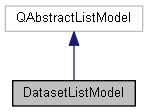
\includegraphics[width=183pt]{class_dataset_list_model__inherit__graph}
\end{center}
\end{figure}


Collaboration diagram for Dataset\+List\+Model\+:\nopagebreak
\begin{figure}[H]
\begin{center}
\leavevmode
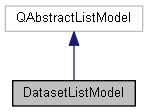
\includegraphics[width=183pt]{class_dataset_list_model__coll__graph}
\end{center}
\end{figure}
\subsection*{Signals}
\begin{DoxyCompactItemize}
\item 
\hypertarget{class_dataset_list_model_a86428aaae4fe37364d16b95c1a40415c}{void {\bfseries Dataset\+Added} (const Q\+Model\+Index \&index)}\label{class_dataset_list_model_a86428aaae4fe37364d16b95c1a40415c}

\end{DoxyCompactItemize}
\subsection*{Public Member Functions}
\begin{DoxyCompactItemize}
\item 
\hypertarget{class_dataset_list_model_a276029a6806e8aef718dd6c2aed05a06}{{\bfseries Dataset\+List\+Model} (Q\+Object $\ast$parent, \hyperlink{class_vespucci_workspace}{Vespucci\+Workspace} $\ast$ws)}\label{class_dataset_list_model_a276029a6806e8aef718dd6c2aed05a06}

\item 
\hypertarget{class_dataset_list_model_a03e20ece69419b89e5c048ec01272c94}{int {\bfseries row\+Count} (const Q\+Model\+Index \&parent) const }\label{class_dataset_list_model_a03e20ece69419b89e5c048ec01272c94}

\item 
\hypertarget{class_dataset_list_model_a4b31feaaf22d48d90ec70a8c20bb0d90}{bool {\bfseries remove\+Row} (int row, const Q\+Model\+Index \&parent)}\label{class_dataset_list_model_a4b31feaaf22d48d90ec70a8c20bb0d90}

\item 
\hypertarget{class_dataset_list_model_a9a186b0ff39cae3bb3b50fab95cd4e43}{bool {\bfseries Add\+Dataset} (Q\+Shared\+Pointer$<$ \hyperlink{class_vespucci_dataset}{Vespucci\+Dataset} $>$ dataset)}\label{class_dataset_list_model_a9a186b0ff39cae3bb3b50fab95cd4e43}

\item 
\hypertarget{class_dataset_list_model_af66b4812c85933aedd7fdccff61a98a0}{Q\+Shared\+Pointer$<$ \hyperlink{class_vespucci_dataset}{Vespucci\+Dataset} $>$ {\bfseries Dataset\+At} (int row)}\label{class_dataset_list_model_af66b4812c85933aedd7fdccff61a98a0}

\item 
Q\+Variant \hyperlink{class_dataset_list_model_af7ce31fef1181dd3e4cac94c754edd05}{data} (const Q\+Model\+Index \&index, int role) const 
\begin{DoxyCompactList}\small\item\em \hyperlink{class_dataset_list_model_af7ce31fef1181dd3e4cac94c754edd05}{Dataset\+List\+Model\+::data}. \end{DoxyCompactList}\item 
\hypertarget{class_dataset_list_model_a2839a86d8b45aaaefbbab118bc954ca0}{void \hyperlink{class_dataset_list_model_a2839a86d8b45aaaefbbab118bc954ca0}{Clear\+Datasets} ()}\label{class_dataset_list_model_a2839a86d8b45aaaefbbab118bc954ca0}

\begin{DoxyCompactList}\small\item\em Dataset\+List\+Model\+::\+Clear\+Mapss Clears the dataset container. Used when closing the program. \end{DoxyCompactList}\end{DoxyCompactItemize}


\subsection{Detailed Description}
The \hyperlink{class_dataset_list_model}{Dataset\+List\+Model} class Exposes the U\+I to the contents of the master dataset list. 

Definition at line 31 of file datasetlistmodel.\+h.



\subsection{Member Function Documentation}
\hypertarget{class_dataset_list_model_af7ce31fef1181dd3e4cac94c754edd05}{\index{Dataset\+List\+Model@{Dataset\+List\+Model}!data@{data}}
\index{data@{data}!Dataset\+List\+Model@{Dataset\+List\+Model}}
\subsubsection[{data}]{\setlength{\rightskip}{0pt plus 5cm}Q\+Variant Dataset\+List\+Model\+::data (
\begin{DoxyParamCaption}
\item[{const Q\+Model\+Index \&}]{index, }
\item[{int}]{role}
\end{DoxyParamCaption}
) const}}\label{class_dataset_list_model_af7ce31fef1181dd3e4cac94c754edd05}


\hyperlink{class_dataset_list_model_af7ce31fef1181dd3e4cac94c754edd05}{Dataset\+List\+Model\+::data}. 


\begin{DoxyParams}{Parameters}
{\em index} & \\
\hline
{\em role} & The role (will always be Qt\+::\+Display\+Role (to display dataset name) \\
\hline
\end{DoxyParams}
\begin{DoxyReturn}{Returns}
A re-\/implementation of Q\+Abstract\+Item\+Model\+::data(); 
\end{DoxyReturn}


Definition at line 40 of file datasetlistmodel.\+cpp.



The documentation for this class was generated from the following files\+:\begin{DoxyCompactItemize}
\item 
C\+:/\+Projects/\+Vespucci/develop/\+G\+U\+I/\+Q\+Abstract\+Item\+Model/datasetlistmodel.\+h\item 
C\+:/\+Projects/\+Vespucci/develop/\+G\+U\+I/\+Q\+Abstract\+Item\+Model/datasetlistmodel.\+cpp\end{DoxyCompactItemize}

\hypertarget{class_dataset_loader}{}\section{Dataset\+Loader Class Reference}
\label{class_dataset_loader}\index{Dataset\+Loader@{Dataset\+Loader}}


The \hyperlink{class_dataset_loader}{Dataset\+Loader} class This class loads the \hyperlink{namespace_vespucci}{Vespucci} Dataset archive (a Z\+IP file saved as .vds) The constructor initializes the Qua\+Zip object corresponding the the archive. The manifest is loaded using Load\+Manifest(); The Y\+A\+ML data in the manifest is parsed by yaml-\/cpp into and the structures are populated by their keys and empty matrices. The empty matrices are then loaded from the .bin files using Load\+Objects.  




{\ttfamily \#include $<$datasetloader.\+h$>$}

\subsection*{Public Member Functions}
\begin{DoxyCompactItemize}
\item 
\hyperlink{class_dataset_loader_ab5fb686a79243a7335fa72ed708a7c7e}{Dataset\+Loader} (Q\+String filename)
\begin{DoxyCompactList}\small\item\em \hyperlink{class_dataset_loader_ab5fb686a79243a7335fa72ed708a7c7e}{Dataset\+Loader\+::\+Dataset\+Loader}. \end{DoxyCompactList}\item 
bool \hyperlink{class_dataset_loader_a7d541be8857c2187a2145d15c1d91346}{Get\+Data} (Q\+Map$<$ Q\+String, mat $>$ \&core\+\_\+objects, Q\+Map$<$ Q\+String, Q\+Map$<$ Q\+String, mat $>$ $>$ \&calcualted\+\_\+objects, Q\+Map$<$ Q\+String, Q\+String $>$ \&metadata)
\begin{DoxyCompactList}\small\item\em \hyperlink{class_dataset_loader_a7d541be8857c2187a2145d15c1d91346}{Dataset\+Loader\+::\+Get\+Data}. \end{DoxyCompactList}\end{DoxyCompactItemize}


\subsection{Detailed Description}
The \hyperlink{class_dataset_loader}{Dataset\+Loader} class This class loads the \hyperlink{namespace_vespucci}{Vespucci} Dataset archive (a Z\+IP file saved as .vds) The constructor initializes the Qua\+Zip object corresponding the the archive. The manifest is loaded using Load\+Manifest(); The Y\+A\+ML data in the manifest is parsed by yaml-\/cpp into and the structures are populated by their keys and empty matrices. The empty matrices are then loaded from the .bin files using Load\+Objects. 

Definition at line 40 of file datasetloader.\+h.



\subsection{Constructor \& Destructor Documentation}
\index{Dataset\+Loader@{Dataset\+Loader}!Dataset\+Loader@{Dataset\+Loader}}
\index{Dataset\+Loader@{Dataset\+Loader}!Dataset\+Loader@{Dataset\+Loader}}
\subsubsection[{\texorpdfstring{Dataset\+Loader(\+Q\+String filename)}{DatasetLoader(QString filename)}}]{\setlength{\rightskip}{0pt plus 5cm}Dataset\+Loader\+::\+Dataset\+Loader (
\begin{DoxyParamCaption}
\item[{Q\+String}]{filename}
\end{DoxyParamCaption}
)}\hypertarget{class_dataset_loader_ab5fb686a79243a7335fa72ed708a7c7e}{}\label{class_dataset_loader_ab5fb686a79243a7335fa72ed708a7c7e}


\hyperlink{class_dataset_loader_ab5fb686a79243a7335fa72ed708a7c7e}{Dataset\+Loader\+::\+Dataset\+Loader}. 


\begin{DoxyParams}{Parameters}
{\em filename} & \\
\hline
\end{DoxyParams}


Definition at line 26 of file datasetloader.\+cpp.



\subsection{Member Function Documentation}
\index{Dataset\+Loader@{Dataset\+Loader}!Get\+Data@{Get\+Data}}
\index{Get\+Data@{Get\+Data}!Dataset\+Loader@{Dataset\+Loader}}
\subsubsection[{\texorpdfstring{Get\+Data(\+Q\+Map$<$ Q\+String, mat $>$ \&core\+\_\+objects, Q\+Map$<$ Q\+String, Q\+Map$<$ Q\+String, mat $>$ $>$ \&calcualted\+\_\+objects, Q\+Map$<$ Q\+String, Q\+String $>$ \&metadata)}{GetData(QMap< QString, mat > &core_objects, QMap< QString, QMap< QString, mat > > &calcualted_objects, QMap< QString, QString > &metadata)}}]{\setlength{\rightskip}{0pt plus 5cm}bool Dataset\+Loader\+::\+Get\+Data (
\begin{DoxyParamCaption}
\item[{Q\+Map$<$ Q\+String, mat $>$ \&}]{core\+\_\+objects, }
\item[{Q\+Map$<$ Q\+String, Q\+Map$<$ Q\+String, mat $>$ $>$ \&}]{calcualted\+\_\+objects, }
\item[{Q\+Map$<$ Q\+String, Q\+String $>$ \&}]{metadata}
\end{DoxyParamCaption}
)}\hypertarget{class_dataset_loader_a7d541be8857c2187a2145d15c1d91346}{}\label{class_dataset_loader_a7d541be8857c2187a2145d15c1d91346}


\hyperlink{class_dataset_loader_a7d541be8857c2187a2145d15c1d91346}{Dataset\+Loader\+::\+Get\+Data}. 


\begin{DoxyParams}{Parameters}
{\em core\+\_\+objects} & \\
\hline
{\em calcualted\+\_\+objects} & \\
\hline
{\em metadata} & Returns the loaded data The \hyperlink{class_vespucci_dataset}{Vespucci\+Dataset} object that spawned this object uses this function to initialize its members \\
\hline
\end{DoxyParams}


Definition at line 72 of file datasetloader.\+cpp.



The documentation for this class was generated from the following files\+:\begin{DoxyCompactItemize}
\item 
Vespucci/\+Data/\+Import/datasetloader.\+h\item 
Vespucci/\+Data/\+Import/datasetloader.\+cpp\end{DoxyCompactItemize}

\hypertarget{class_dataset_saver}{}\section{Dataset\+Saver Class Reference}
\label{class_dataset_saver}\index{Dataset\+Saver@{Dataset\+Saver}}
\subsection*{Public Member Functions}
\begin{DoxyCompactItemize}
\item 
{\bfseries Dataset\+Saver} (Q\+Shared\+Pointer$<$ \hyperlink{class_vespucci_dataset}{Vespucci\+Dataset} $>$ dataset)\hypertarget{class_dataset_saver_a544eaca6a91a4943e053b0a53477d9b6}{}\label{class_dataset_saver_a544eaca6a91a4943e053b0a53477d9b6}

\end{DoxyCompactItemize}


\subsection{Detailed Description}


Definition at line 26 of file datasetsaver.\+h.



The documentation for this class was generated from the following files\+:\begin{DoxyCompactItemize}
\item 
Vespucci/\+Data/\+Import/datasetsaver.\+h\item 
Vespucci/\+Data/\+Import/datasetsaver.\+cpp\end{DoxyCompactItemize}

\hypertarget{class_dataset_tree_model}{}\section{Dataset\+Tree\+Model Class Reference}
\label{class_dataset_tree_model}\index{Dataset\+Tree\+Model@{Dataset\+Tree\+Model}}
Inheritance diagram for Dataset\+Tree\+Model\+:\begin{figure}[H]
\begin{center}
\leavevmode
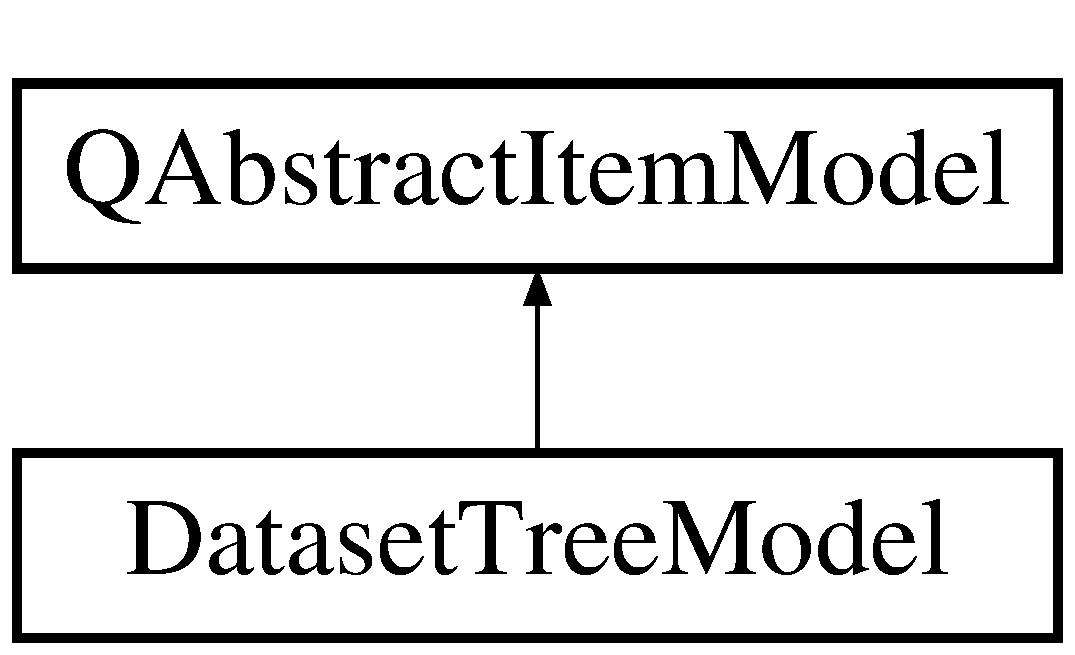
\includegraphics[height=2.000000cm]{class_dataset_tree_model}
\end{center}
\end{figure}
\subsection*{Public Member Functions}
\begin{DoxyCompactItemize}
\item 
{\bfseries Dataset\+Tree\+Model} (Q\+Object $\ast$parent)\hypertarget{class_dataset_tree_model_ab5225c75a58682f12bed8eeb5342d57c}{}\label{class_dataset_tree_model_ab5225c75a58682f12bed8eeb5342d57c}

\item 
{\bfseries Dataset\+Tree\+Model} (Q\+Object $\ast$parent, const \hyperlink{class_data_model}{Data\+Model} $\ast$data\+\_\+model)\hypertarget{class_dataset_tree_model_af1085ae203d04401068a43e29f93584e}{}\label{class_dataset_tree_model_af1085ae203d04401068a43e29f93584e}

\item 
void \hyperlink{class_dataset_tree_model_a6b790c46fce2661df22f977568747799}{Setup\+Model\+Data} (const \hyperlink{class_data_model}{Data\+Model} $\ast$data\+\_\+model)
\begin{DoxyCompactList}\small\item\em \hyperlink{class_dataset_tree_model_a6b790c46fce2661df22f977568747799}{Dataset\+Tree\+Model\+::\+Setup\+Model\+Data}. \end{DoxyCompactList}\item 
Q\+Variant {\bfseries data} (const Q\+Model\+Index \&index, int role) const Q\+\_\+\+D\+E\+C\+L\+\_\+\+O\+V\+E\+R\+R\+I\+DE\hypertarget{class_dataset_tree_model_abee1d278c2e76b6f758f5ecf60a58609}{}\label{class_dataset_tree_model_abee1d278c2e76b6f758f5ecf60a58609}

\item 
Qt\+::\+Item\+Flags {\bfseries flags} (const Q\+Model\+Index \&index) const Q\+\_\+\+D\+E\+C\+L\+\_\+\+O\+V\+E\+R\+R\+I\+DE\hypertarget{class_dataset_tree_model_a2a121ff1099f33efc89e85274b234d69}{}\label{class_dataset_tree_model_a2a121ff1099f33efc89e85274b234d69}

\item 
Q\+Variant {\bfseries header\+Data} (int section, Qt\+::\+Orientation orientation, int role=Qt\+::\+Display\+Role) const Q\+\_\+\+D\+E\+C\+L\+\_\+\+O\+V\+E\+R\+R\+I\+DE\hypertarget{class_dataset_tree_model_acaedaa126d810cf90e8428e656667281}{}\label{class_dataset_tree_model_acaedaa126d810cf90e8428e656667281}

\item 
Q\+Model\+Index {\bfseries index} (int row, int column, const Q\+Model\+Index \&parent=Q\+Model\+Index()) const Q\+\_\+\+D\+E\+C\+L\+\_\+\+O\+V\+E\+R\+R\+I\+DE\hypertarget{class_dataset_tree_model_ad77d80cbb89b328c1e4b907f75d97bb7}{}\label{class_dataset_tree_model_ad77d80cbb89b328c1e4b907f75d97bb7}

\item 
Q\+Model\+Index {\bfseries parent} (const Q\+Model\+Index \&index) const Q\+\_\+\+D\+E\+C\+L\+\_\+\+O\+V\+E\+R\+R\+I\+DE\hypertarget{class_dataset_tree_model_a0632356b4a79219f07957f0934dce29a}{}\label{class_dataset_tree_model_a0632356b4a79219f07957f0934dce29a}

\item 
int {\bfseries row\+Count} (const Q\+Model\+Index \&parent) const Q\+\_\+\+D\+E\+C\+L\+\_\+\+O\+V\+E\+R\+R\+I\+DE\hypertarget{class_dataset_tree_model_ad88f002ac8bc88099867ff68d19d383e}{}\label{class_dataset_tree_model_ad88f002ac8bc88099867ff68d19d383e}

\item 
int {\bfseries column\+Count} (const Q\+Model\+Index \&parent) const Q\+\_\+\+D\+E\+C\+L\+\_\+\+O\+V\+E\+R\+R\+I\+DE\hypertarget{class_dataset_tree_model_a731a037c013492069bc701824fe7155c}{}\label{class_dataset_tree_model_a731a037c013492069bc701824fe7155c}

\item 
bool {\bfseries remove\+Rows} (int row, int count, const Q\+Model\+Index \&parent=Q\+Model\+Index()) Q\+\_\+\+D\+E\+C\+L\+\_\+\+O\+V\+E\+R\+R\+I\+DE\hypertarget{class_dataset_tree_model_ae7707a7eca291896295e238809016d77}{}\label{class_dataset_tree_model_ae7707a7eca291896295e238809016d77}

\item 
void {\bfseries Update\+Data} (const \hyperlink{class_data_model}{Data\+Model} $\ast$data\+\_\+model)\hypertarget{class_dataset_tree_model_a2e05e6b5953aad5921a29e643f977c53}{}\label{class_dataset_tree_model_a2e05e6b5953aad5921a29e643f977c53}

\item 
void {\bfseries Add\+Dataset} (Q\+Shared\+Pointer$<$ \hyperlink{class_vespucci_dataset}{Vespucci\+Dataset} $>$ dataset)\hypertarget{class_dataset_tree_model_ac43ddd0aefecc9434dabce31728e8d7d}{}\label{class_dataset_tree_model_ac43ddd0aefecc9434dabce31728e8d7d}

\item 
bool {\bfseries Is\+Matrix} (const Q\+Model\+Index \&index)\hypertarget{class_dataset_tree_model_acff63b8d7b909efa12869d836e855aa4}{}\label{class_dataset_tree_model_acff63b8d7b909efa12869d836e855aa4}

\item 
bool {\bfseries Is\+Dataset} (const Q\+Model\+Index \&index)\hypertarget{class_dataset_tree_model_a4f32fc47d886e44b34a77778d07df8b2}{}\label{class_dataset_tree_model_a4f32fc47d886e44b34a77778d07df8b2}

\item 
bool {\bfseries Is\+Map} (const Q\+Model\+Index \&index)\hypertarget{class_dataset_tree_model_a9f9e4ebe9abbfc218ba3a769aa43d4db}{}\label{class_dataset_tree_model_a9f9e4ebe9abbfc218ba3a769aa43d4db}

\item 
void {\bfseries Clear\+Datasets} ()\hypertarget{class_dataset_tree_model_a02b02368a2f2528902265e0e3805471c}{}\label{class_dataset_tree_model_a02b02368a2f2528902265e0e3805471c}

\item 
void {\bfseries remove\+Row} (const Q\+Model\+Index \&index)\hypertarget{class_dataset_tree_model_a12c19482931a5aba1506952469639d1c}{}\label{class_dataset_tree_model_a12c19482931a5aba1506952469639d1c}

\item 
\hyperlink{class_tree_item}{Tree\+Item} $\ast$ {\bfseries get\+Item} (const Q\+Model\+Index \&index) const \hypertarget{class_dataset_tree_model_a2a190008fdbf1bcca5dca0bacb430aaa}{}\label{class_dataset_tree_model_a2a190008fdbf1bcca5dca0bacb430aaa}

\item 
\hyperlink{class_tree_item}{Tree\+Item} $\ast$ {\bfseries root\+\_\+item} ()\hypertarget{class_dataset_tree_model_a66f44fb2740195500a7d6ff6ae2079a2}{}\label{class_dataset_tree_model_a66f44fb2740195500a7d6ff6ae2079a2}

\end{DoxyCompactItemize}


\subsection{Detailed Description}


Definition at line 33 of file datasettreemodel.\+h.



\subsection{Member Function Documentation}
\index{Dataset\+Tree\+Model@{Dataset\+Tree\+Model}!Setup\+Model\+Data@{Setup\+Model\+Data}}
\index{Setup\+Model\+Data@{Setup\+Model\+Data}!Dataset\+Tree\+Model@{Dataset\+Tree\+Model}}
\subsubsection[{\texorpdfstring{Setup\+Model\+Data(const Data\+Model $\ast$data\+\_\+model)}{SetupModelData(const DataModel *data_model)}}]{\setlength{\rightskip}{0pt plus 5cm}void Dataset\+Tree\+Model\+::\+Setup\+Model\+Data (
\begin{DoxyParamCaption}
\item[{const {\bf Data\+Model} $\ast$}]{data\+\_\+model}
\end{DoxyParamCaption}
)}\hypertarget{class_dataset_tree_model_a6b790c46fce2661df22f977568747799}{}\label{class_dataset_tree_model_a6b790c46fce2661df22f977568747799}


\hyperlink{class_dataset_tree_model_a6b790c46fce2661df22f977568747799}{Dataset\+Tree\+Model\+::\+Setup\+Model\+Data}. 


\begin{DoxyParams}{Parameters}
{\em data\+\_\+model} & Can throw an exception if one is thrown by data\+\_\+model-\/$>$Get\+Dataset() \\
\hline
\end{DoxyParams}


Definition at line 128 of file datasettreemodel.\+cpp.



The documentation for this class was generated from the following files\+:\begin{DoxyCompactItemize}
\item 
Vespucci/\+G\+U\+I/\+Q\+Abstract\+Item\+Model/datasettreemodel.\+h\item 
Vespucci/\+G\+U\+I/\+Q\+Abstract\+Item\+Model/datasettreemodel.\+cpp\end{DoxyCompactItemize}

\hypertarget{class_data_viewer}{}\section{Data\+Viewer Class Reference}
\label{class_data_viewer}\index{Data\+Viewer@{Data\+Viewer}}


The \hyperlink{class_data_viewer}{Data\+Viewer} class Window that displays dataset elements in a Q\+Table\+View widget inside a Q\+Tab\+Widget.  




{\ttfamily \#include $<$dataviewer.\+h$>$}

Inheritance diagram for Data\+Viewer\+:\begin{figure}[H]
\begin{center}
\leavevmode
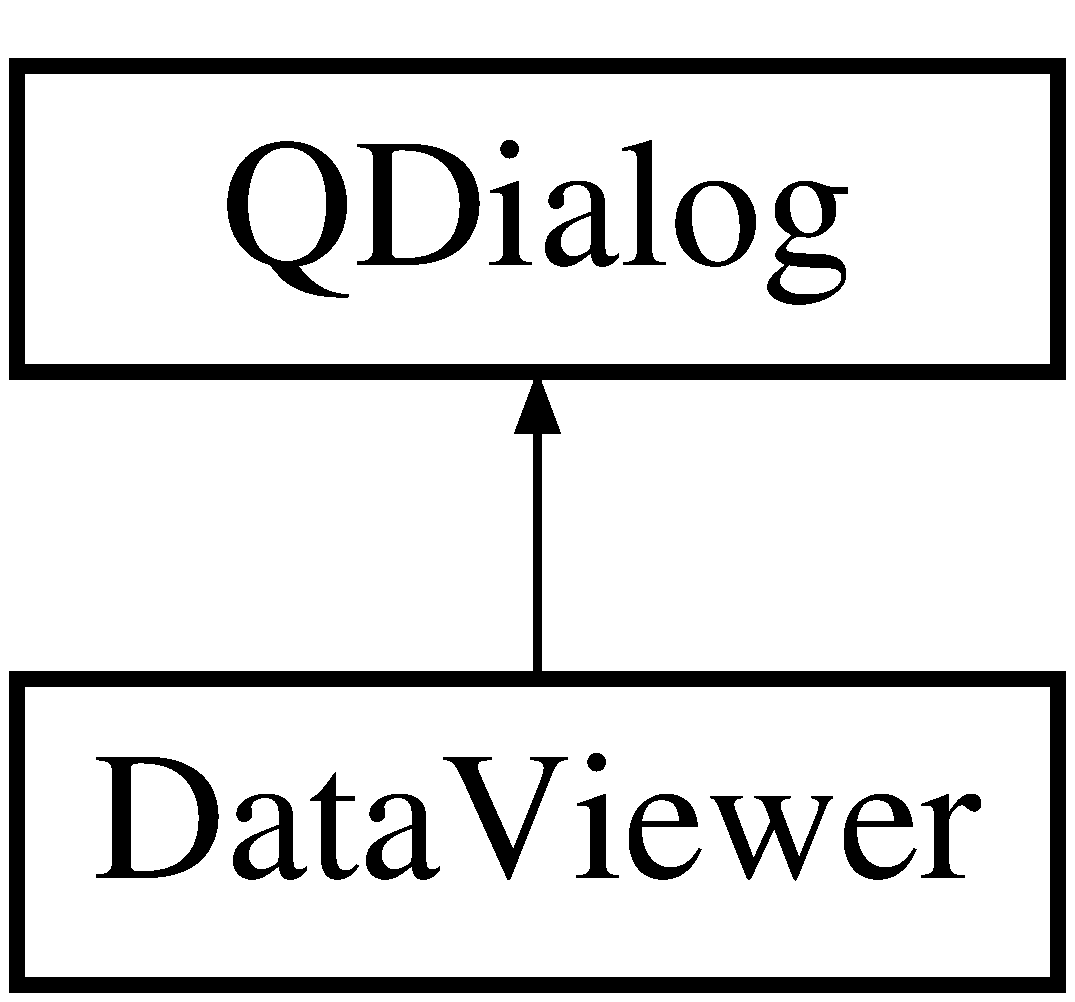
\includegraphics[height=2.000000cm]{class_data_viewer}
\end{center}
\end{figure}
\subsection*{Public Slots}
\begin{DoxyCompactItemize}
\item 
void {\bfseries Remove\+Tab} (int index)\hypertarget{class_data_viewer_a1fc3adf11c33af30e2592277566029a7}{}\label{class_data_viewer_a1fc3adf11c33af30e2592277566029a7}

\end{DoxyCompactItemize}
\subsection*{Public Member Functions}
\begin{DoxyCompactItemize}
\item 
\hyperlink{class_data_viewer_a01e88d2b8a54711550dd5ee10eda415c}{Data\+Viewer} (\hyperlink{class_main_window}{Main\+Window} $\ast$parent=0)
\begin{DoxyCompactList}\small\item\em \hyperlink{class_data_viewer_a01e88d2b8a54711550dd5ee10eda415c}{Data\+Viewer\+::\+Data\+Viewer}. \end{DoxyCompactList}\item 
void {\bfseries Add\+Tab} (const mat \&object, const Q\+String \&name)\hypertarget{class_data_viewer_a10dcaec63874d3ffa5ac2fee93ef3142}{}\label{class_data_viewer_a10dcaec63874d3ffa5ac2fee93ef3142}

\item 
const mat \& {\bfseries Empty\+Matrix} ()\hypertarget{class_data_viewer_ac0924576701ca847da0caeddabe4e4b0}{}\label{class_data_viewer_ac0924576701ca847da0caeddabe4e4b0}

\end{DoxyCompactItemize}


\subsection{Detailed Description}
The \hyperlink{class_data_viewer}{Data\+Viewer} class Window that displays dataset elements in a Q\+Table\+View widget inside a Q\+Tab\+Widget. 

Definition at line 41 of file dataviewer.\+h.



\subsection{Constructor \& Destructor Documentation}
\index{Data\+Viewer@{Data\+Viewer}!Data\+Viewer@{Data\+Viewer}}
\index{Data\+Viewer@{Data\+Viewer}!Data\+Viewer@{Data\+Viewer}}
\subsubsection[{\texorpdfstring{Data\+Viewer(\+Main\+Window $\ast$parent=0)}{DataViewer(MainWindow *parent=0)}}]{\setlength{\rightskip}{0pt plus 5cm}Data\+Viewer\+::\+Data\+Viewer (
\begin{DoxyParamCaption}
\item[{{\bf Main\+Window} $\ast$}]{parent = {\ttfamily 0}}
\end{DoxyParamCaption}
)\hspace{0.3cm}{\ttfamily [explicit]}}\hypertarget{class_data_viewer_a01e88d2b8a54711550dd5ee10eda415c}{}\label{class_data_viewer_a01e88d2b8a54711550dd5ee10eda415c}


\hyperlink{class_data_viewer_a01e88d2b8a54711550dd5ee10eda415c}{Data\+Viewer\+::\+Data\+Viewer}. 


\begin{DoxyParams}{Parameters}
{\em parent} & Usually \hyperlink{class_main_window}{Main\+Window}, because ther \\
\hline
{\em ws} & The \char`\"{}global\char`\"{} workspace, provides access to other dialogs \\
\hline
\end{DoxyParams}


Definition at line 29 of file dataviewer.\+cpp.



The documentation for this class was generated from the following files\+:\begin{DoxyCompactItemize}
\item 
Vespucci/\+G\+U\+I/\+Display/dataviewer.\+h\item 
Vespucci/\+G\+U\+I/\+Display/dataviewer.\+cpp\end{DoxyCompactItemize}

\hypertarget{class_data_widget}{}\section{Data\+Widget Class Reference}
\label{class_data_widget}\index{Data\+Widget@{Data\+Widget}}
Inheritance diagram for Data\+Widget\+:\begin{figure}[H]
\begin{center}
\leavevmode
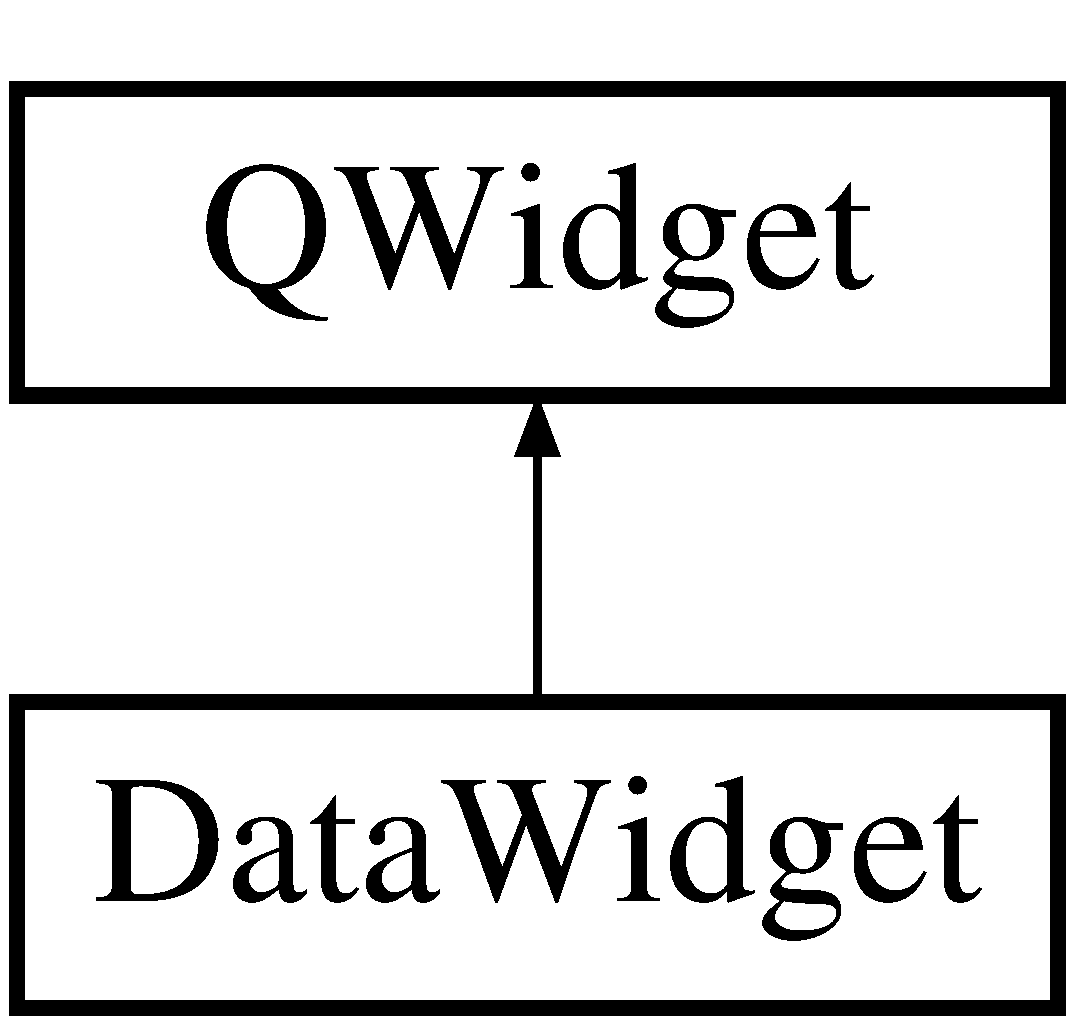
\includegraphics[height=2.000000cm]{class_data_widget}
\end{center}
\end{figure}
\subsection*{Public Member Functions}
\begin{DoxyCompactItemize}
\item 
{\bfseries Data\+Widget} (Q\+Widget $\ast$parent, \hyperlink{class_vespucci_table_model}{Vespucci\+Table\+Model} $\ast$table\+\_\+model)\hypertarget{class_data_widget_a174ea64da70aa2804acdb3fe2cfdf36f}{}\label{class_data_widget_a174ea64da70aa2804acdb3fe2cfdf36f}

\item 
void {\bfseries Set\+Table\+Model} (\hyperlink{class_vespucci_table_model}{Vespucci\+Table\+Model} $\ast$table\+\_\+model)\hypertarget{class_data_widget_a67dff1faa11bde1cecff0608c3856301}{}\label{class_data_widget_a67dff1faa11bde1cecff0608c3856301}

\item 
\hyperlink{class_vespucci_table_model}{Vespucci\+Table\+Model} $\ast$ {\bfseries Get\+Table\+Model} ()\hypertarget{class_data_widget_ac2a4a6e07971f424b5243b00f0b28fd4}{}\label{class_data_widget_ac2a4a6e07971f424b5243b00f0b28fd4}

\end{DoxyCompactItemize}


\subsection{Detailed Description}


Definition at line 30 of file datawidget.\+h.



The documentation for this class was generated from the following files\+:\begin{DoxyCompactItemize}
\item 
Vespucci/\+G\+U\+I/\+Display/datawidget.\+h\item 
Vespucci/\+G\+U\+I/\+Display/datawidget.\+cpp\end{DoxyCompactItemize}

\hypertarget{class_vespucci_1_1_math_1_1_distance_metric_wrapper}{}\section{Vespucci\+:\+:Math\+:\+:Distance\+Metric\+Wrapper Class Reference}
\label{class_vespucci_1_1_math_1_1_distance_metric_wrapper}\index{Vespucci\+::\+Math\+::\+Distance\+Metric\+Wrapper@{Vespucci\+::\+Math\+::\+Distance\+Metric\+Wrapper}}
\subsection*{Public Member Functions}
\begin{DoxyCompactItemize}
\item 
{\bfseries Distance\+Metric\+Wrapper} (std\+::string metric\+\_\+description)\hypertarget{class_vespucci_1_1_math_1_1_distance_metric_wrapper_ab06269d2b9546a7bd11b24ee26e524ba}{}\label{class_vespucci_1_1_math_1_1_distance_metric_wrapper_ab06269d2b9546a7bd11b24ee26e524ba}

\item 
double {\bfseries Evaluate} (arma\+::vec \&first, arma\+::vec \&second)\hypertarget{class_vespucci_1_1_math_1_1_distance_metric_wrapper_a5d50b09c4f454f6dd0caf855a97318e0}{}\label{class_vespucci_1_1_math_1_1_distance_metric_wrapper_a5d50b09c4f454f6dd0caf855a97318e0}

\end{DoxyCompactItemize}


\subsection{Detailed Description}


Definition at line 27 of file distancemetricwrapper.\+h.



The documentation for this class was generated from the following files\+:\begin{DoxyCompactItemize}
\item 
Vespucci\+Library/include/\+Math/\+Accessory/distancemetricwrapper.\+h\item 
Vespucci\+Library/src/\+Math/\+Accessory/distancemetricwrapper.\+cpp\end{DoxyCompactItemize}

\hypertarget{class_vespucci_1_1_external_1_1_file_interprocess}{}\section{Vespucci\+:\+:External\+:\+:File\+Interprocess Class Reference}
\label{class_vespucci_1_1_external_1_1_file_interprocess}\index{Vespucci\+::\+External\+::\+File\+Interprocess@{Vespucci\+::\+External\+::\+File\+Interprocess}}
\subsection*{Public Slots}
\begin{DoxyCompactItemize}
\item 
void {\bfseries Process\+Finished} ()\hypertarget{class_vespucci_1_1_external_1_1_file_interprocess_a787da5e18d2ca4fe872f6f19917bc303}{}\label{class_vespucci_1_1_external_1_1_file_interprocess_a787da5e18d2ca4fe872f6f19917bc303}

\end{DoxyCompactItemize}
\subsection*{Public Member Functions}
\begin{DoxyCompactItemize}
\item 
{\bfseries File\+Interprocess} (const arma\+::field$<$ std\+::string $>$ invar\+\_\+names, const arma\+::field$<$ arma\+::mat $>$ invars, const arma\+::field$<$ std\+::string $>$ outvar\+\_\+names)\hypertarget{class_vespucci_1_1_external_1_1_file_interprocess_a49a06a227a2835e4af5ef33f535d5e7a}{}\label{class_vespucci_1_1_external_1_1_file_interprocess_a49a06a227a2835e4af5ef33f535d5e7a}

\item 
arma\+::field$<$ arma\+::mat $>$ {\bfseries outvars} ()\hypertarget{class_vespucci_1_1_external_1_1_file_interprocess_a42dca33ce869eb5827dd335f70eec9a3}{}\label{class_vespucci_1_1_external_1_1_file_interprocess_a42dca33ce869eb5827dd335f70eec9a3}

\item 
int {\bfseries RunR} (const std\+::string \&script, const Q\+String \&R\+\_\+\+H\+O\+ME)\hypertarget{class_vespucci_1_1_external_1_1_file_interprocess_a3fbf26155a33758f13e8000a2dad8053}{}\label{class_vespucci_1_1_external_1_1_file_interprocess_a3fbf26155a33758f13e8000a2dad8053}

\item 
int {\bfseries Run\+Octave} (const std\+::string \&script)\hypertarget{class_vespucci_1_1_external_1_1_file_interprocess_abd9df6f2d481568272aa54cfe05001b9}{}\label{class_vespucci_1_1_external_1_1_file_interprocess_abd9df6f2d481568272aa54cfe05001b9}

\end{DoxyCompactItemize}


\subsection{Detailed Description}


Definition at line 7 of file fileinterprocess.\+h.



The documentation for this class was generated from the following files\+:\begin{DoxyCompactItemize}
\item 
Vespucci/\+External/fileinterprocess.\+h\item 
Vespucci/\+External/fileinterprocess.\+cpp\end{DoxyCompactItemize}

\hypertarget{class_filter_dialog}{}\section{Filter\+Dialog Class Reference}
\label{class_filter_dialog}\index{Filter\+Dialog@{Filter\+Dialog}}


The \hyperlink{class_filter_dialog}{Filter\+Dialog} class This dialog allows the user to apply filtering, smoothing or derivatization to the dataset.  




{\ttfamily \#include $<$filterdialog.\+h$>$}

Inheritance diagram for Filter\+Dialog\+:\begin{figure}[H]
\begin{center}
\leavevmode
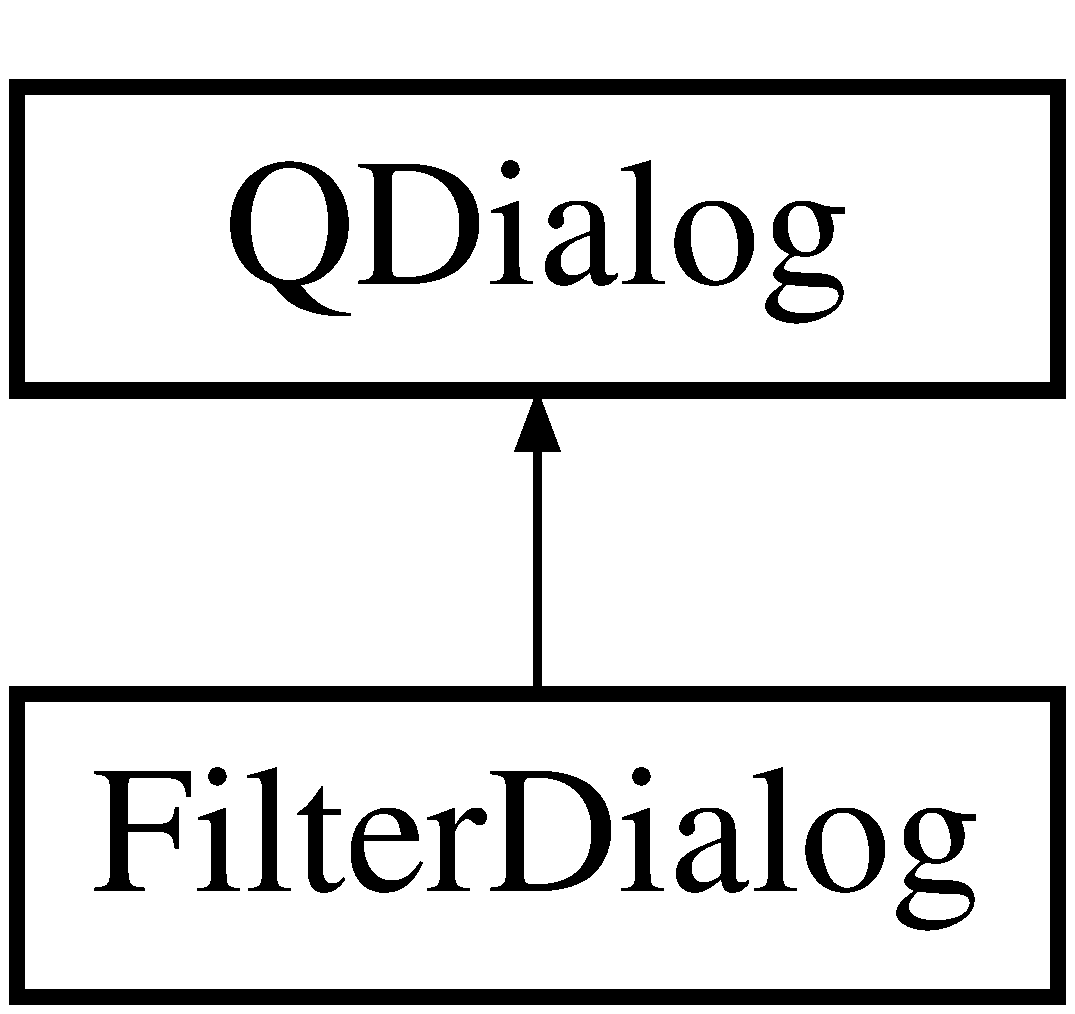
\includegraphics[height=2.000000cm]{class_filter_dialog}
\end{center}
\end{figure}
\subsection*{Public Member Functions}
\begin{DoxyCompactItemize}
\item 
\hyperlink{class_filter_dialog_a62e2170f1487851d7aba6a0f63820bae}{Filter\+Dialog} (Q\+Widget $\ast$parent, \hyperlink{class_vespucci_workspace}{Vespucci\+Workspace} $\ast$ws, const Q\+String \&dataset\+\_\+key)
\begin{DoxyCompactList}\small\item\em \hyperlink{class_filter_dialog_a62e2170f1487851d7aba6a0f63820bae}{Filter\+Dialog\+::\+Filter\+Dialog}. \end{DoxyCompactList}\end{DoxyCompactItemize}


\subsection{Detailed Description}
The \hyperlink{class_filter_dialog}{Filter\+Dialog} class This dialog allows the user to apply filtering, smoothing or derivatization to the dataset. 

Definition at line 37 of file filterdialog.\+h.



\subsection{Constructor \& Destructor Documentation}
\index{Filter\+Dialog@{Filter\+Dialog}!Filter\+Dialog@{Filter\+Dialog}}
\index{Filter\+Dialog@{Filter\+Dialog}!Filter\+Dialog@{Filter\+Dialog}}
\subsubsection[{\texorpdfstring{Filter\+Dialog(\+Q\+Widget $\ast$parent, Vespucci\+Workspace $\ast$ws, const Q\+String \&dataset\+\_\+key)}{FilterDialog(QWidget *parent, VespucciWorkspace *ws, const QString &dataset_key)}}]{\setlength{\rightskip}{0pt plus 5cm}Filter\+Dialog\+::\+Filter\+Dialog (
\begin{DoxyParamCaption}
\item[{Q\+Widget $\ast$}]{parent, }
\item[{{\bf Vespucci\+Workspace} $\ast$}]{ws, }
\item[{const Q\+String \&}]{dataset\+\_\+key}
\end{DoxyParamCaption}
)\hspace{0.3cm}{\ttfamily [explicit]}}\hypertarget{class_filter_dialog_a62e2170f1487851d7aba6a0f63820bae}{}\label{class_filter_dialog_a62e2170f1487851d7aba6a0f63820bae}


\hyperlink{class_filter_dialog_a62e2170f1487851d7aba6a0f63820bae}{Filter\+Dialog\+::\+Filter\+Dialog}. 


\begin{DoxyParams}{Parameters}
{\em parent} & Parent Q\+Widget \\
\hline
{\em ws} & Current workspace \\
\hline
{\em row} & Row of current dataset \\
\hline
\end{DoxyParams}


Definition at line 29 of file filterdialog.\+cpp.



The documentation for this class was generated from the following files\+:\begin{DoxyCompactItemize}
\item 
Vespucci/\+G\+U\+I/\+Processing/filterdialog.\+h\item 
Vespucci/\+G\+U\+I/\+Processing/filterdialog.\+cpp\end{DoxyCompactItemize}

\hypertarget{class_fourier_transform_dialog}{}\section{Fourier\+Transform\+Dialog Class Reference}
\label{class_fourier_transform_dialog}\index{Fourier\+Transform\+Dialog@{Fourier\+Transform\+Dialog}}
Inheritance diagram for Fourier\+Transform\+Dialog\+:\begin{figure}[H]
\begin{center}
\leavevmode
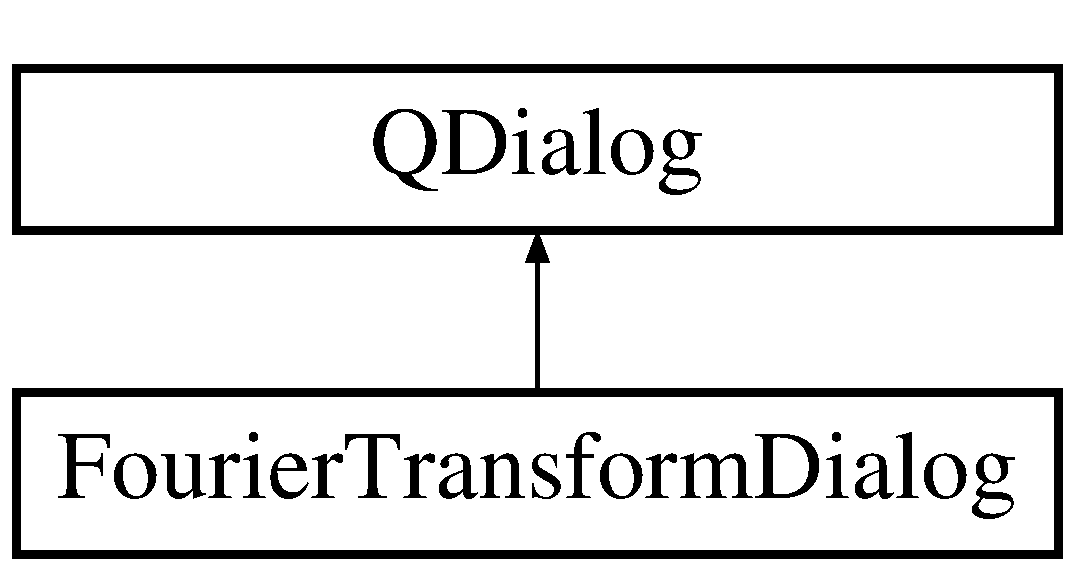
\includegraphics[height=2.000000cm]{class_fourier_transform_dialog}
\end{center}
\end{figure}
\subsection*{Public Member Functions}
\begin{DoxyCompactItemize}
\item 
{\bfseries Fourier\+Transform\+Dialog} (Q\+Widget $\ast$parent, \hyperlink{class_vespucci_workspace}{Vespucci\+Workspace} $\ast$ws, const Q\+String \&dataset\+\_\+key)\hypertarget{class_fourier_transform_dialog_a4c5347a86c5fc9d701b489039ef0dd1c}{}\label{class_fourier_transform_dialog_a4c5347a86c5fc9d701b489039ef0dd1c}

\end{DoxyCompactItemize}


\subsection{Detailed Description}


Definition at line 10 of file fouriertransformdialog.\+h.



The documentation for this class was generated from the following files\+:\begin{DoxyCompactItemize}
\item 
Vespucci/\+G\+U\+I/\+Processing/fouriertransformdialog.\+h\item 
Vespucci/\+G\+U\+I/\+Processing/fouriertransformdialog.\+cpp\end{DoxyCompactItemize}

\hypertarget{class_vespucci_1_1_external_1_1_interprocess_sender}{}\section{Vespucci\+:\+:External\+:\+:Interprocess\+Sender Class Reference}
\label{class_vespucci_1_1_external_1_1_interprocess_sender}\index{Vespucci\+::\+External\+::\+Interprocess\+Sender@{Vespucci\+::\+External\+::\+Interprocess\+Sender}}
\subsection*{Public Member Functions}
\begin{DoxyCompactItemize}
\item 
{\bfseries Interprocess\+Sender} (std\+::map$<$ std\+::string, arma\+::mat $\ast$ $>$ invars, std\+::vector$<$ std\+::string $>$ outvar\+\_\+names)\hypertarget{class_vespucci_1_1_external_1_1_interprocess_sender_aea180357ec2e0b47d4077e8781a96873}{}\label{class_vespucci_1_1_external_1_1_interprocess_sender_aea180357ec2e0b47d4077e8781a96873}

\item 
bool {\bfseries Send\+To\+Octave} (std\+::string command)\hypertarget{class_vespucci_1_1_external_1_1_interprocess_sender_a6c76ed36f384c8369cc2a5da45888d99}{}\label{class_vespucci_1_1_external_1_1_interprocess_sender_a6c76ed36f384c8369cc2a5da45888d99}

\item 
bool {\bfseries Send\+ToR} (std\+::string command)\hypertarget{class_vespucci_1_1_external_1_1_interprocess_sender_ac1e68c293b66eb376ef006a64acc4665}{}\label{class_vespucci_1_1_external_1_1_interprocess_sender_ac1e68c293b66eb376ef006a64acc4665}

\item 
std\+::map$<$ std\+::string, arma\+::mat $>$ {\bfseries Get\+Values} ()\hypertarget{class_vespucci_1_1_external_1_1_interprocess_sender_a0954ee3010a9020791eb32c5fb9343b9}{}\label{class_vespucci_1_1_external_1_1_interprocess_sender_a0954ee3010a9020791eb32c5fb9343b9}

\end{DoxyCompactItemize}


\subsection{Detailed Description}


Definition at line 7 of file interprocesssender.\+h.



The documentation for this class was generated from the following files\+:\begin{DoxyCompactItemize}
\item 
Vespucci/\+External/interprocesssender.\+h\item 
Vespucci/\+External/interprocesssender.\+cpp\end{DoxyCompactItemize}

\hypertarget{class_k_means_dialog}{\section{K\+Means\+Dialog Class Reference}
\label{class_k_means_dialog}\index{K\+Means\+Dialog@{K\+Means\+Dialog}}
}


The \hyperlink{class_k_means_dialog}{K\+Means\+Dialog} class Allows the user to create a k-\/means clustering map.  




{\ttfamily \#include $<$kmeansdialog.\+h$>$}



Inheritance diagram for K\+Means\+Dialog\+:\nopagebreak
\begin{figure}[H]
\begin{center}
\leavevmode
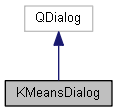
\includegraphics[width=160pt]{class_k_means_dialog__inherit__graph}
\end{center}
\end{figure}


Collaboration diagram for K\+Means\+Dialog\+:\nopagebreak
\begin{figure}[H]
\begin{center}
\leavevmode
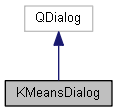
\includegraphics[width=160pt]{class_k_means_dialog__coll__graph}
\end{center}
\end{figure}
\subsection*{Public Member Functions}
\begin{DoxyCompactItemize}
\item 
\hyperlink{class_k_means_dialog_aabbd83299a966eb6e64e74d4333845c8}{K\+Means\+Dialog} (Q\+Widget $\ast$parent, \hyperlink{class_vespucci_workspace}{Vespucci\+Workspace} $\ast$ws, int row)
\begin{DoxyCompactList}\small\item\em \hyperlink{class_k_means_dialog_aabbd83299a966eb6e64e74d4333845c8}{K\+Means\+Dialog\+::\+K\+Means\+Dialog}. \end{DoxyCompactList}\end{DoxyCompactItemize}


\subsection{Detailed Description}
The \hyperlink{class_k_means_dialog}{K\+Means\+Dialog} class Allows the user to create a k-\/means clustering map. 

Definition at line 33 of file kmeansdialog.\+h.



\subsection{Constructor \& Destructor Documentation}
\hypertarget{class_k_means_dialog_aabbd83299a966eb6e64e74d4333845c8}{\index{K\+Means\+Dialog@{K\+Means\+Dialog}!K\+Means\+Dialog@{K\+Means\+Dialog}}
\index{K\+Means\+Dialog@{K\+Means\+Dialog}!K\+Means\+Dialog@{K\+Means\+Dialog}}
\subsubsection[{K\+Means\+Dialog}]{\setlength{\rightskip}{0pt plus 5cm}K\+Means\+Dialog\+::\+K\+Means\+Dialog (
\begin{DoxyParamCaption}
\item[{Q\+Widget $\ast$}]{parent, }
\item[{{\bf Vespucci\+Workspace} $\ast$}]{ws, }
\item[{int}]{row}
\end{DoxyParamCaption}
)\hspace{0.3cm}{\ttfamily [explicit]}}}\label{class_k_means_dialog_aabbd83299a966eb6e64e74d4333845c8}


\hyperlink{class_k_means_dialog_aabbd83299a966eb6e64e74d4333845c8}{K\+Means\+Dialog\+::\+K\+Means\+Dialog}. 


\begin{DoxyParams}{Parameters}
{\em parent} & Parent Q\+Widget \\
\hline
{\em ws} & Current workspace \\
\hline
{\em row} & Row of current dataset \\
\hline
\end{DoxyParams}


Definition at line 29 of file kmeansdialog.\+cpp.



The documentation for this class was generated from the following files\+:\begin{DoxyCompactItemize}
\item 
C\+:/\+Projects/\+Vespucci/develop/\+G\+U\+I/\+Analysis/kmeansdialog.\+h\item 
C\+:/\+Projects/\+Vespucci/develop/\+G\+U\+I/\+Analysis/kmeansdialog.\+cpp\end{DoxyCompactItemize}

\hypertarget{class_load_dataset}{}\section{Load\+Dataset Class Reference}
\label{class_load_dataset}\index{Load\+Dataset@{Load\+Dataset}}


The \hyperlink{class_load_dataset}{Load\+Dataset} class Dialog that allows the user to import files into the program.  




{\ttfamily \#include $<$loaddataset.\+h$>$}

Inheritance diagram for Load\+Dataset\+:\begin{figure}[H]
\begin{center}
\leavevmode
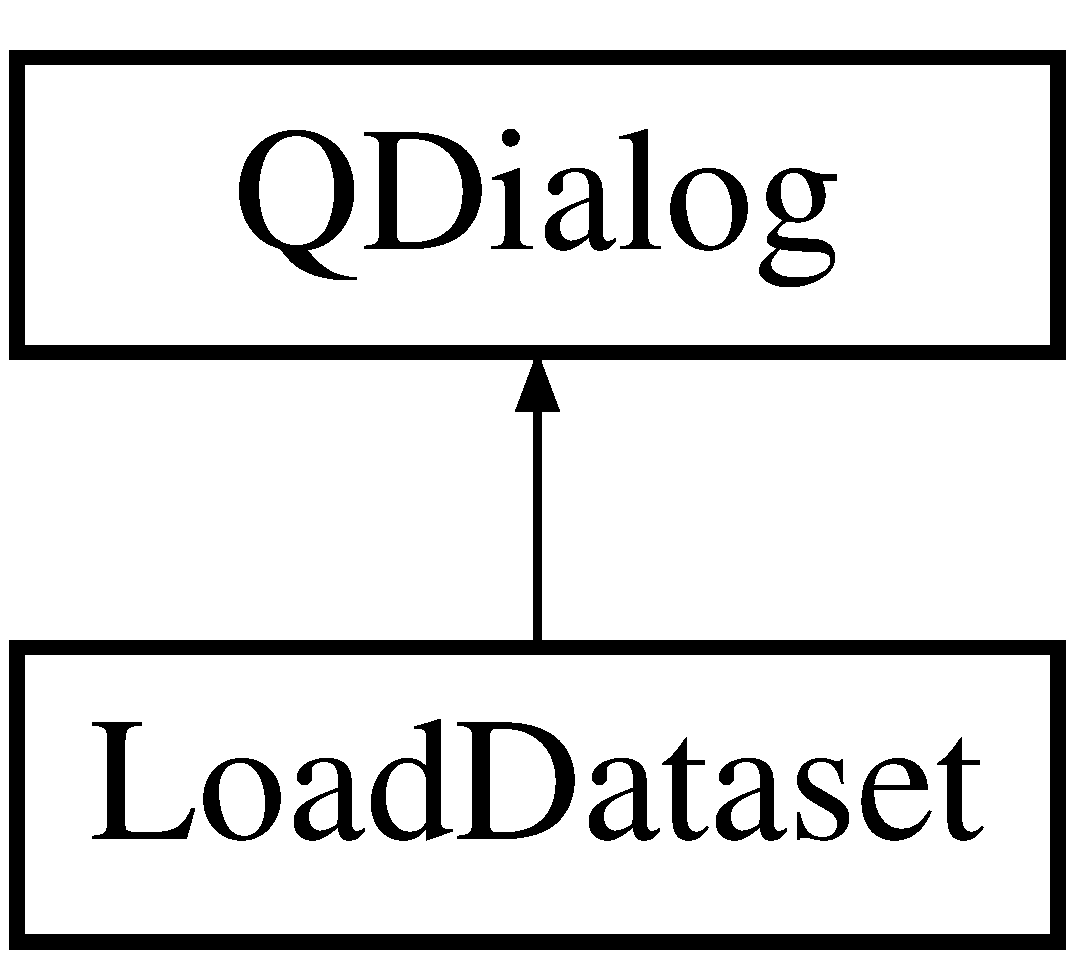
\includegraphics[height=2.000000cm]{class_load_dataset}
\end{center}
\end{figure}
\subsection*{Public Slots}
\begin{DoxyCompactItemize}
\item 
void {\bfseries Filename\+Changed} (Q\+String new\+\_\+filename)\hypertarget{class_load_dataset_ac9fa943d881a92fac675753e85207da9}{}\label{class_load_dataset_ac9fa943d881a92fac675753e85207da9}

\end{DoxyCompactItemize}
\subsection*{Public Member Functions}
\begin{DoxyCompactItemize}
\item 
\hyperlink{class_load_dataset_a23139475dbcb8e5d44ba83fe46621334}{Load\+Dataset} (Q\+Widget $\ast$parent, \hyperlink{class_vespucci_workspace}{Vespucci\+Workspace} $\ast$ws)
\begin{DoxyCompactList}\small\item\em \hyperlink{class_load_dataset_a23139475dbcb8e5d44ba83fe46621334}{Load\+Dataset\+::\+Load\+Dataset}. \end{DoxyCompactList}\end{DoxyCompactItemize}


\subsection{Detailed Description}
The \hyperlink{class_load_dataset}{Load\+Dataset} class Dialog that allows the user to import files into the program. 

Definition at line 33 of file loaddataset.\+h.



\subsection{Constructor \& Destructor Documentation}
\index{Load\+Dataset@{Load\+Dataset}!Load\+Dataset@{Load\+Dataset}}
\index{Load\+Dataset@{Load\+Dataset}!Load\+Dataset@{Load\+Dataset}}
\subsubsection[{\texorpdfstring{Load\+Dataset(\+Q\+Widget $\ast$parent, Vespucci\+Workspace $\ast$ws)}{LoadDataset(QWidget *parent, VespucciWorkspace *ws)}}]{\setlength{\rightskip}{0pt plus 5cm}Load\+Dataset\+::\+Load\+Dataset (
\begin{DoxyParamCaption}
\item[{Q\+Widget $\ast$}]{parent, }
\item[{{\bf Vespucci\+Workspace} $\ast$}]{ws}
\end{DoxyParamCaption}
)\hspace{0.3cm}{\ttfamily [explicit]}}\hypertarget{class_load_dataset_a23139475dbcb8e5d44ba83fe46621334}{}\label{class_load_dataset_a23139475dbcb8e5d44ba83fe46621334}


\hyperlink{class_load_dataset_a23139475dbcb8e5d44ba83fe46621334}{Load\+Dataset\+::\+Load\+Dataset}. 


\begin{DoxyParams}{Parameters}
{\em parent} & Q\+Widget parent (see Q\+Dialog) \\
\hline
{\em ws} & Current workspace \\
\hline
\end{DoxyParams}


Definition at line 31 of file loaddataset.\+cpp.



The documentation for this class was generated from the following files\+:\begin{DoxyCompactItemize}
\item 
Vespucci/\+G\+U\+I/\+Processing/loaddataset.\+h\item 
Vespucci/\+G\+U\+I/\+Processing/loaddataset.\+cpp\end{DoxyCompactItemize}

\hypertarget{class_macro_dialog}{}\section{Macro\+Dialog Class Reference}
\label{class_macro_dialog}\index{Macro\+Dialog@{Macro\+Dialog}}
Inheritance diagram for Macro\+Dialog\+:\begin{figure}[H]
\begin{center}
\leavevmode
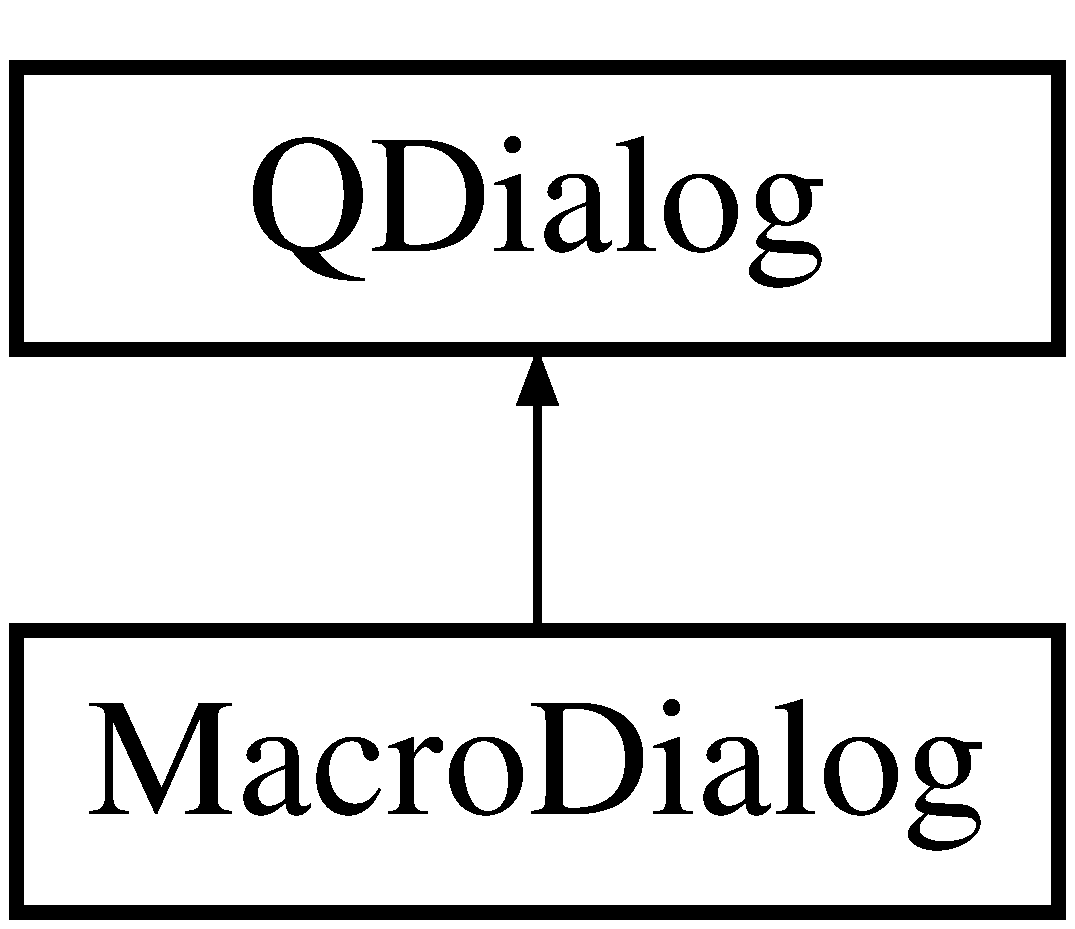
\includegraphics[height=2.000000cm]{class_macro_dialog}
\end{center}
\end{figure}
\subsection*{Public Member Functions}
\begin{DoxyCompactItemize}
\item 
{\bfseries Macro\+Dialog} (\hyperlink{class_main_window}{Main\+Window} $\ast$parent, \hyperlink{class_vespucci_workspace}{Vespucci\+Workspace} $\ast$ws)\hypertarget{class_macro_dialog_a0b0fe1bf78931117107f3e4ed798d501}{}\label{class_macro_dialog_a0b0fe1bf78931117107f3e4ed798d501}

\item 
void {\bfseries Set\+Active\+Dataset} (Q\+Shared\+Pointer$<$ \hyperlink{class_vespucci_dataset}{Vespucci\+Dataset} $>$ dataset)\hypertarget{class_macro_dialog_a9ce87a0218177f83d1927e9554637bde}{}\label{class_macro_dialog_a9ce87a0218177f83d1927e9554637bde}

\end{DoxyCompactItemize}


\subsection{Detailed Description}


Definition at line 32 of file macrodialog.\+h.



The documentation for this class was generated from the following files\+:\begin{DoxyCompactItemize}
\item 
Vespucci/\+G\+U\+I/macrodialog.\+h\item 
Vespucci/\+G\+U\+I/macrodialog.\+cpp\end{DoxyCompactItemize}

\hypertarget{class_macro_parser}{}\section{Macro\+Parser Class Reference}
\label{class_macro_parser}\index{Macro\+Parser@{Macro\+Parser}}
\subsection*{Public Member Functions}
\begin{DoxyCompactItemize}
\item 
{\bfseries Macro\+Parser} (Q\+Shared\+Pointer$<$ \hyperlink{class_vespucci_dataset}{Vespucci\+Dataset} $>$ dataset)\hypertarget{class_macro_parser_a0301a59c269a2fd00d38ce35f7eec58d}{}\label{class_macro_parser_a0301a59c269a2fd00d38ce35f7eec58d}

\item 
bool \hyperlink{class_macro_parser_aa4665646889e62019f894a60b8cff9ec}{Load\+Macro} (Q\+String macro)
\begin{DoxyCompactList}\small\item\em \hyperlink{class_macro_parser_aa4665646889e62019f894a60b8cff9ec}{Macro\+Parser\+::\+Load\+Macro}. \end{DoxyCompactList}\item 
bool \hyperlink{class_macro_parser_a4b2ee20c04071ccb10c9cbca0888c182}{Execute\+Macro} ()\hypertarget{class_macro_parser_a4b2ee20c04071ccb10c9cbca0888c182}{}\label{class_macro_parser_a4b2ee20c04071ccb10c9cbca0888c182}

\begin{DoxyCompactList}\small\item\em \hyperlink{class_macro_parser_a4b2ee20c04071ccb10c9cbca0888c182}{Macro\+Parser\+::\+Execute\+Macro} Iteratively executes the commands in commands\+\_\+. Each command is first validated. If any command is invalid, none execute. The method returns false whenever any invalid command is found. The caller only uses error\+\_\+line and error\+\_\+param if this function returns false. \end{DoxyCompactList}\item 
bool {\bfseries Error} (int \&error\+\_\+line, int \&error\+\_\+param\+\_\+)\hypertarget{class_macro_parser_a3b06ad2c47655d604d30f94699edcedc}{}\label{class_macro_parser_a3b06ad2c47655d604d30f94699edcedc}

\end{DoxyCompactItemize}


\subsection{Detailed Description}


Definition at line 24 of file macroparser.\+h.



\subsection{Member Function Documentation}
\index{Macro\+Parser@{Macro\+Parser}!Load\+Macro@{Load\+Macro}}
\index{Load\+Macro@{Load\+Macro}!Macro\+Parser@{Macro\+Parser}}
\subsubsection[{\texorpdfstring{Load\+Macro(\+Q\+String macro)}{LoadMacro(QString macro)}}]{\setlength{\rightskip}{0pt plus 5cm}bool Macro\+Parser\+::\+Load\+Macro (
\begin{DoxyParamCaption}
\item[{Q\+String}]{macro}
\end{DoxyParamCaption}
)}\hypertarget{class_macro_parser_aa4665646889e62019f894a60b8cff9ec}{}\label{class_macro_parser_aa4665646889e62019f894a60b8cff9ec}


\hyperlink{class_macro_parser_aa4665646889e62019f894a60b8cff9ec}{Macro\+Parser\+::\+Load\+Macro}. 


\begin{DoxyParams}{Parameters}
{\em macro} & Parses string containing the macro. Commands must be separated by newlines and cannot be nested. If not on list of valid commands (or not formatted correctly), User will be warned of syntax err of this returns false \\
\hline
\end{DoxyParams}


Definition at line 36 of file macroparser.\+cpp.



The documentation for this class was generated from the following files\+:\begin{DoxyCompactItemize}
\item 
Vespucci/\+Data/\+Dataset/macroparser.\+h\item 
Vespucci/\+Data/\+Dataset/macroparser.\+cpp\end{DoxyCompactItemize}

\hypertarget{class_main_window}{\section{Main\+Window Class Reference}
\label{class_main_window}\index{Main\+Window@{Main\+Window}}
}


The \hyperlink{class_main_window}{Main\+Window} class The main window of the program, this is where the user performs most operations.  




{\ttfamily \#include $<$mainwindow.\+h$>$}



Inheritance diagram for Main\+Window\+:\nopagebreak
\begin{figure}[H]
\begin{center}
\leavevmode
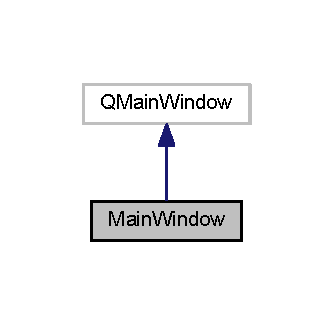
\includegraphics[width=160pt]{class_main_window__inherit__graph}
\end{center}
\end{figure}


Collaboration diagram for Main\+Window\+:\nopagebreak
\begin{figure}[H]
\begin{center}
\leavevmode
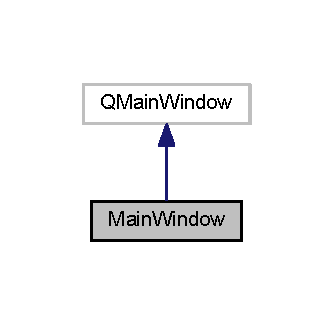
\includegraphics[width=160pt]{class_main_window__coll__graph}
\end{center}
\end{figure}
\subsection*{Public Slots}
\begin{DoxyCompactItemize}
\item 
\hypertarget{class_main_window_aabdd9af63bada1cef223752691c3d8e0}{void {\bfseries Range\+Dialog\+Accepted} (double min, double max)}\label{class_main_window_aabdd9af63bada1cef223752691c3d8e0}

\end{DoxyCompactItemize}
\subsection*{Signals}
\begin{DoxyCompactItemize}
\item 
\hypertarget{class_main_window_ab2c4828c97d36f9dca59d7f0d5314b84}{void {\bfseries Global\+Gradient\+Changed} (Q\+C\+P\+Color\+Gradient gradient)}\label{class_main_window_ab2c4828c97d36f9dca59d7f0d5314b84}

\item 
\hypertarget{class_main_window_a6de945a7ef4b0a52998e1662bfb99c0f}{void {\bfseries Global\+Data\+Range\+Changed} (Q\+C\+P\+Range data\+\_\+range)}\label{class_main_window_a6de945a7ef4b0a52998e1662bfb99c0f}

\end{DoxyCompactItemize}
\subsection*{Public Member Functions}
\begin{DoxyCompactItemize}
\item 
\hyperlink{class_main_window_ab87cdab2f1b7c709fc0f8bca4cf09ebc}{Main\+Window} (Q\+Widget $\ast$parent, \hyperlink{class_vespucci_workspace}{Vespucci\+Workspace} $\ast$ws)
\begin{DoxyCompactList}\small\item\em \hyperlink{class_main_window_ab87cdab2f1b7c709fc0f8bca4cf09ebc}{Main\+Window\+::\+Main\+Window}. \end{DoxyCompactList}\item 
Q\+C\+P\+Range $\ast$ \hyperlink{class_main_window_a89e2dbed5fa59653909d8cd2195c67be}{global\+\_\+data\+\_\+range} ()
\begin{DoxyCompactList}\small\item\em \hyperlink{class_main_window_a89e2dbed5fa59653909d8cd2195c67be}{Main\+Window\+::global\+\_\+data\+\_\+range}. \end{DoxyCompactList}\item 
Q\+C\+P\+Color\+Gradient $\ast$ \hyperlink{class_main_window_abe4c08852fad9c895a712dcd22ac9bd5}{global\+\_\+gradient} ()
\begin{DoxyCompactList}\small\item\em \hyperlink{class_main_window_abe4c08852fad9c895a712dcd22ac9bd5}{Main\+Window\+::global\+\_\+gradient}. \end{DoxyCompactList}\item 
void \hyperlink{class_main_window_a58206491beb13daf24f3ba72e5eebbc0}{Recalculate\+Global\+Data\+Range} (Q\+C\+P\+Range $\ast$new\+\_\+data\+\_\+range)
\begin{DoxyCompactList}\small\item\em \hyperlink{class_main_window_a58206491beb13daf24f3ba72e5eebbc0}{Main\+Window\+::\+Recalculate\+Global\+Data\+Range}. \end{DoxyCompactList}\item 
void \hyperlink{class_main_window_a004bb70b988b902f0e1618bdb2695960}{Refresh\+Global\+Color\+Gradient} (Q\+C\+P\+Color\+Gradient new\+\_\+gradient)
\begin{DoxyCompactList}\small\item\em \hyperlink{class_main_window_a004bb70b988b902f0e1618bdb2695960}{Main\+Window\+::\+Refresh\+Global\+Color\+Gradient}. \end{DoxyCompactList}\item 
void \hyperlink{class_main_window_aa0c431f17d5790a5bfc0e49e429c173b}{Set\+Global\+Data\+Range} (Q\+C\+P\+Range $\ast$new\+\_\+data\+\_\+range)
\begin{DoxyCompactList}\small\item\em \hyperlink{class_main_window_aa0c431f17d5790a5bfc0e49e429c173b}{Main\+Window\+::\+Set\+Global\+Data\+Range}. \end{DoxyCompactList}\item 
\hyperlink{class_vespucci_workspace}{Vespucci\+Workspace} $\ast$ \hyperlink{class_main_window_af78d7dca13e15077306eb27737edb096}{workspace\+\_\+ptr} ()
\begin{DoxyCompactList}\small\item\em \hyperlink{class_main_window_af78d7dca13e15077306eb27737edb096}{Main\+Window\+::workspace\+\_\+ptr}. \end{DoxyCompactList}\item 
void \hyperlink{class_main_window_afe21228ed02306f34b6194cefeeb7feb}{Display\+Exception\+Warning} (std\+::exception e)
\begin{DoxyCompactList}\small\item\em \hyperlink{class_main_window_afe21228ed02306f34b6194cefeeb7feb}{Main\+Window\+::\+Display\+Exception\+Warning}. \end{DoxyCompactList}\item 
\hypertarget{class_main_window_a7a13630a02a40927bfb218078c586f9f}{Q\+List\+View $\ast$ {\bfseries map\+\_\+list\+\_\+view} ()}\label{class_main_window_a7a13630a02a40927bfb218078c586f9f}

\item 
void \hyperlink{class_main_window_a2961ddb7545da22e3bb0df7aca85bae1}{Set\+Active\+Dataset\+List\+Row} (int row)
\begin{DoxyCompactList}\small\item\em \hyperlink{class_main_window_a2961ddb7545da22e3bb0df7aca85bae1}{Main\+Window\+::\+Set\+Active\+Dataset\+List\+Row}. \end{DoxyCompactList}\item 
\hypertarget{class_main_window_ad31a733d5590bebf61af8413b6251a06}{bool {\bfseries Dataset\+Mappable} (int row)}\label{class_main_window_ad31a733d5590bebf61af8413b6251a06}

\end{DoxyCompactItemize}
\subsection*{Protected Member Functions}
\begin{DoxyCompactItemize}
\item 
void \hyperlink{class_main_window_a4e20a4a065fbb0e4d3532a45a0a91425}{close\+Event} (Q\+Close\+Event $\ast$event)
\begin{DoxyCompactList}\small\item\em \hyperlink{class_main_window_a4e20a4a065fbb0e4d3532a45a0a91425}{Main\+Window\+::close\+Event}. \end{DoxyCompactList}\end{DoxyCompactItemize}


\subsection{Detailed Description}
The \hyperlink{class_main_window}{Main\+Window} class The main window of the program, this is where the user performs most operations. 

Definition at line 38 of file mainwindow.\+h.



\subsection{Constructor \& Destructor Documentation}
\hypertarget{class_main_window_ab87cdab2f1b7c709fc0f8bca4cf09ebc}{\index{Main\+Window@{Main\+Window}!Main\+Window@{Main\+Window}}
\index{Main\+Window@{Main\+Window}!Main\+Window@{Main\+Window}}
\subsubsection[{Main\+Window}]{\setlength{\rightskip}{0pt plus 5cm}Main\+Window\+::\+Main\+Window (
\begin{DoxyParamCaption}
\item[{Q\+Widget $\ast$}]{parent, }
\item[{{\bf Vespucci\+Workspace} $\ast$}]{ws}
\end{DoxyParamCaption}
)\hspace{0.3cm}{\ttfamily [explicit]}}}\label{class_main_window_ab87cdab2f1b7c709fc0f8bca4cf09ebc}


\hyperlink{class_main_window_ab87cdab2f1b7c709fc0f8bca4cf09ebc}{Main\+Window\+::\+Main\+Window}. 


\begin{DoxyParams}{Parameters}
{\em parent} & usually 0 \\
\hline
{\em ws} & the workspace of this instance of \hyperlink{namespace_vespucci}{Vespucci} Default constructor \\
\hline
\end{DoxyParams}


Definition at line 54 of file mainwindow.\+cpp.



Here is the call graph for this function\+:\nopagebreak
\begin{figure}[H]
\begin{center}
\leavevmode
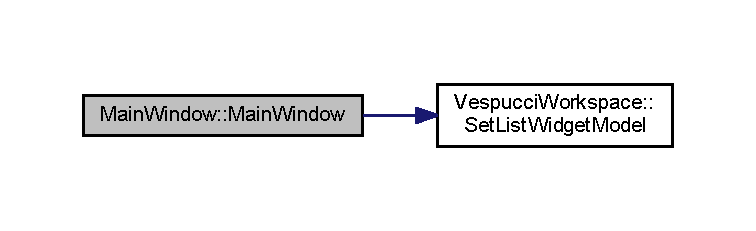
\includegraphics[width=350pt]{class_main_window_ab87cdab2f1b7c709fc0f8bca4cf09ebc_cgraph}
\end{center}
\end{figure}




\subsection{Member Function Documentation}
\hypertarget{class_main_window_a4e20a4a065fbb0e4d3532a45a0a91425}{\index{Main\+Window@{Main\+Window}!close\+Event@{close\+Event}}
\index{close\+Event@{close\+Event}!Main\+Window@{Main\+Window}}
\subsubsection[{close\+Event}]{\setlength{\rightskip}{0pt plus 5cm}void Main\+Window\+::close\+Event (
\begin{DoxyParamCaption}
\item[{Q\+Close\+Event $\ast$}]{event}
\end{DoxyParamCaption}
)\hspace{0.3cm}{\ttfamily [protected]}}}\label{class_main_window_a4e20a4a065fbb0e4d3532a45a0a91425}


\hyperlink{class_main_window_a4e20a4a065fbb0e4d3532a45a0a91425}{Main\+Window\+::close\+Event}. 


\begin{DoxyParams}{Parameters}
{\em event} & Exits the program \\
\hline
\end{DoxyParams}


Definition at line 77 of file mainwindow.\+cpp.



Here is the call graph for this function\+:\nopagebreak
\begin{figure}[H]
\begin{center}
\leavevmode
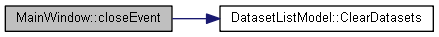
\includegraphics[width=350pt]{class_main_window_a4e20a4a065fbb0e4d3532a45a0a91425_cgraph}
\end{center}
\end{figure}


\hypertarget{class_main_window_afe21228ed02306f34b6194cefeeb7feb}{\index{Main\+Window@{Main\+Window}!Display\+Exception\+Warning@{Display\+Exception\+Warning}}
\index{Display\+Exception\+Warning@{Display\+Exception\+Warning}!Main\+Window@{Main\+Window}}
\subsubsection[{Display\+Exception\+Warning}]{\setlength{\rightskip}{0pt plus 5cm}void Main\+Window\+::\+Display\+Exception\+Warning (
\begin{DoxyParamCaption}
\item[{std\+::exception}]{e}
\end{DoxyParamCaption}
)}}\label{class_main_window_afe21228ed02306f34b6194cefeeb7feb}


\hyperlink{class_main_window_afe21228ed02306f34b6194cefeeb7feb}{Main\+Window\+::\+Display\+Exception\+Warning}. 


\begin{DoxyParams}{Parameters}
{\em e} & Used to handle exceptions arising from dialogs. Displays a pop-\/up box describing the nature of the error. Most exceptions are not critical, but will result in the action that caused the exception being canceled. \\
\hline
\end{DoxyParams}


Definition at line 804 of file mainwindow.\+cpp.



Here is the caller graph for this function\+:\nopagebreak
\begin{figure}[H]
\begin{center}
\leavevmode
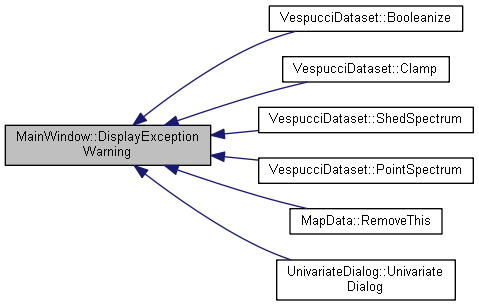
\includegraphics[width=350pt]{class_main_window_afe21228ed02306f34b6194cefeeb7feb_icgraph}
\end{center}
\end{figure}


\hypertarget{class_main_window_a89e2dbed5fa59653909d8cd2195c67be}{\index{Main\+Window@{Main\+Window}!global\+\_\+data\+\_\+range@{global\+\_\+data\+\_\+range}}
\index{global\+\_\+data\+\_\+range@{global\+\_\+data\+\_\+range}!Main\+Window@{Main\+Window}}
\subsubsection[{global\+\_\+data\+\_\+range}]{\setlength{\rightskip}{0pt plus 5cm}Q\+C\+P\+Range $\ast$ Main\+Window\+::global\+\_\+data\+\_\+range (
\begin{DoxyParamCaption}
{}
\end{DoxyParamCaption}
)}}\label{class_main_window_a89e2dbed5fa59653909d8cd2195c67be}


\hyperlink{class_main_window_a89e2dbed5fa59653909d8cd2195c67be}{Main\+Window\+::global\+\_\+data\+\_\+range}. 

\begin{DoxyReturn}{Returns}
Return the global data range (to \hyperlink{class_map_viewer}{Map\+Viewer} widgets) 
\end{DoxyReturn}


Definition at line 706 of file mainwindow.\+cpp.



Here is the call graph for this function\+:\nopagebreak
\begin{figure}[H]
\begin{center}
\leavevmode
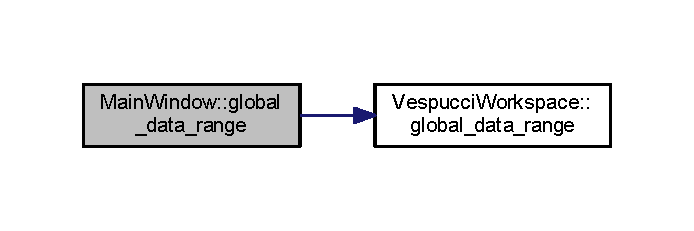
\includegraphics[width=333pt]{class_main_window_a89e2dbed5fa59653909d8cd2195c67be_cgraph}
\end{center}
\end{figure}




Here is the caller graph for this function\+:\nopagebreak
\begin{figure}[H]
\begin{center}
\leavevmode
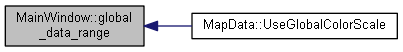
\includegraphics[width=350pt]{class_main_window_a89e2dbed5fa59653909d8cd2195c67be_icgraph}
\end{center}
\end{figure}


\hypertarget{class_main_window_abe4c08852fad9c895a712dcd22ac9bd5}{\index{Main\+Window@{Main\+Window}!global\+\_\+gradient@{global\+\_\+gradient}}
\index{global\+\_\+gradient@{global\+\_\+gradient}!Main\+Window@{Main\+Window}}
\subsubsection[{global\+\_\+gradient}]{\setlength{\rightskip}{0pt plus 5cm}Q\+C\+P\+Color\+Gradient $\ast$ Main\+Window\+::global\+\_\+gradient (
\begin{DoxyParamCaption}
{}
\end{DoxyParamCaption}
)}}\label{class_main_window_abe4c08852fad9c895a712dcd22ac9bd5}


\hyperlink{class_main_window_abe4c08852fad9c895a712dcd22ac9bd5}{Main\+Window\+::global\+\_\+gradient}. 

\begin{DoxyReturn}{Returns}
Return the global color gradient (to \hyperlink{class_map_viewer}{Map\+Viewer} widgets) 
\end{DoxyReturn}


Definition at line 715 of file mainwindow.\+cpp.



Here is the call graph for this function\+:\nopagebreak
\begin{figure}[H]
\begin{center}
\leavevmode
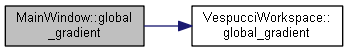
\includegraphics[width=333pt]{class_main_window_abe4c08852fad9c895a712dcd22ac9bd5_cgraph}
\end{center}
\end{figure}




Here is the caller graph for this function\+:\nopagebreak
\begin{figure}[H]
\begin{center}
\leavevmode
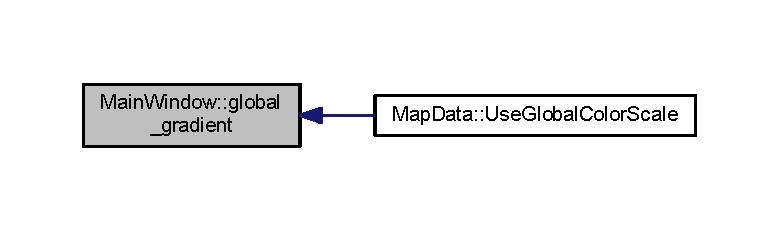
\includegraphics[width=350pt]{class_main_window_abe4c08852fad9c895a712dcd22ac9bd5_icgraph}
\end{center}
\end{figure}


\hypertarget{class_main_window_a58206491beb13daf24f3ba72e5eebbc0}{\index{Main\+Window@{Main\+Window}!Recalculate\+Global\+Data\+Range@{Recalculate\+Global\+Data\+Range}}
\index{Recalculate\+Global\+Data\+Range@{Recalculate\+Global\+Data\+Range}!Main\+Window@{Main\+Window}}
\subsubsection[{Recalculate\+Global\+Data\+Range}]{\setlength{\rightskip}{0pt plus 5cm}void Main\+Window\+::\+Recalculate\+Global\+Data\+Range (
\begin{DoxyParamCaption}
\item[{Q\+C\+P\+Range $\ast$}]{new\+\_\+data\+\_\+range}
\end{DoxyParamCaption}
)}}\label{class_main_window_a58206491beb13daf24f3ba72e5eebbc0}


\hyperlink{class_main_window_a58206491beb13daf24f3ba72e5eebbc0}{Main\+Window\+::\+Recalculate\+Global\+Data\+Range}. 


\begin{DoxyParams}{Parameters}
{\em new\+\_\+data\+\_\+range} & Recalculate the global data range based on previous range and the new data \\
\hline
\end{DoxyParams}


Definition at line 724 of file mainwindow.\+cpp.



Here is the call graph for this function\+:\nopagebreak
\begin{figure}[H]
\begin{center}
\leavevmode
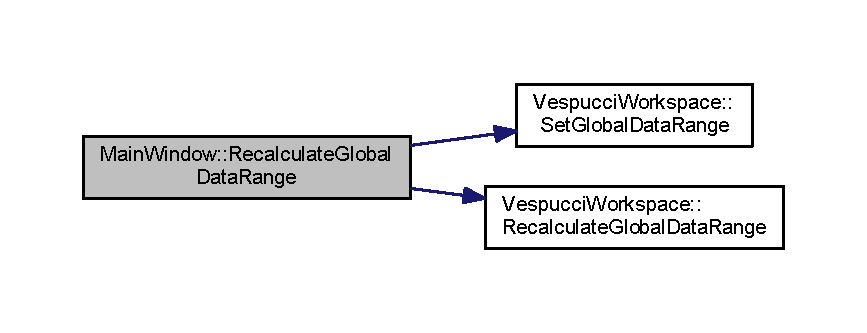
\includegraphics[width=350pt]{class_main_window_a58206491beb13daf24f3ba72e5eebbc0_cgraph}
\end{center}
\end{figure}




Here is the caller graph for this function\+:\nopagebreak
\begin{figure}[H]
\begin{center}
\leavevmode
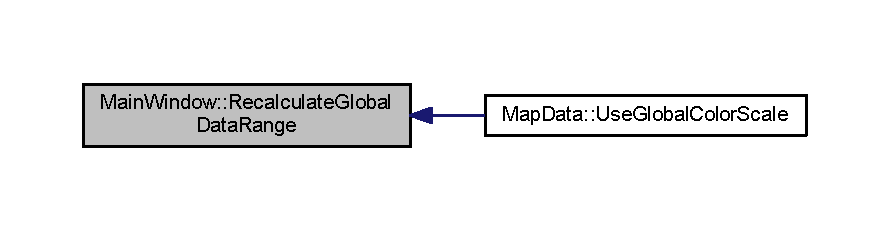
\includegraphics[width=350pt]{class_main_window_a58206491beb13daf24f3ba72e5eebbc0_icgraph}
\end{center}
\end{figure}


\hypertarget{class_main_window_a004bb70b988b902f0e1618bdb2695960}{\index{Main\+Window@{Main\+Window}!Refresh\+Global\+Color\+Gradient@{Refresh\+Global\+Color\+Gradient}}
\index{Refresh\+Global\+Color\+Gradient@{Refresh\+Global\+Color\+Gradient}!Main\+Window@{Main\+Window}}
\subsubsection[{Refresh\+Global\+Color\+Gradient}]{\setlength{\rightskip}{0pt plus 5cm}void Main\+Window\+::\+Refresh\+Global\+Color\+Gradient (
\begin{DoxyParamCaption}
\item[{Q\+C\+P\+Color\+Gradient}]{new\+\_\+gradient}
\end{DoxyParamCaption}
)}}\label{class_main_window_a004bb70b988b902f0e1618bdb2695960}


\hyperlink{class_main_window_a004bb70b988b902f0e1618bdb2695960}{Main\+Window\+::\+Refresh\+Global\+Color\+Gradient}. 


\begin{DoxyParams}{Parameters}
{\em new\+\_\+gradient} & Change the global color gradient and update it for all objects using it \\
\hline
\end{DoxyParams}


Definition at line 741 of file mainwindow.\+cpp.



Here is the call graph for this function\+:\nopagebreak
\begin{figure}[H]
\begin{center}
\leavevmode
\includegraphics[width=350pt]{class_main_window_a004bb70b988b902f0e1618bdb2695960_cgraph}
\end{center}
\end{figure}


\hypertarget{class_main_window_a2961ddb7545da22e3bb0df7aca85bae1}{\index{Main\+Window@{Main\+Window}!Set\+Active\+Dataset\+List\+Row@{Set\+Active\+Dataset\+List\+Row}}
\index{Set\+Active\+Dataset\+List\+Row@{Set\+Active\+Dataset\+List\+Row}!Main\+Window@{Main\+Window}}
\subsubsection[{Set\+Active\+Dataset\+List\+Row}]{\setlength{\rightskip}{0pt plus 5cm}void Main\+Window\+::\+Set\+Active\+Dataset\+List\+Row (
\begin{DoxyParamCaption}
\item[{int}]{row}
\end{DoxyParamCaption}
)}}\label{class_main_window_a2961ddb7545da22e3bb0df7aca85bae1}


\hyperlink{class_main_window_a2961ddb7545da22e3bb0df7aca85bae1}{Main\+Window\+::\+Set\+Active\+Dataset\+List\+Row}. 


\begin{DoxyParams}{Parameters}
{\em row} & Change the row that is active in the dataset list view \\
\hline
\end{DoxyParams}


Definition at line 827 of file mainwindow.\+cpp.

\hypertarget{class_main_window_aa0c431f17d5790a5bfc0e49e429c173b}{\index{Main\+Window@{Main\+Window}!Set\+Global\+Data\+Range@{Set\+Global\+Data\+Range}}
\index{Set\+Global\+Data\+Range@{Set\+Global\+Data\+Range}!Main\+Window@{Main\+Window}}
\subsubsection[{Set\+Global\+Data\+Range}]{\setlength{\rightskip}{0pt plus 5cm}void Main\+Window\+::\+Set\+Global\+Data\+Range (
\begin{DoxyParamCaption}
\item[{Q\+C\+P\+Range $\ast$}]{new\+\_\+data\+\_\+range}
\end{DoxyParamCaption}
)}}\label{class_main_window_aa0c431f17d5790a5bfc0e49e429c173b}


\hyperlink{class_main_window_aa0c431f17d5790a5bfc0e49e429c173b}{Main\+Window\+::\+Set\+Global\+Data\+Range}. 


\begin{DoxyParams}{Parameters}
{\em new\+\_\+data\+\_\+range} & Set the global data range and update it for all objects using it \\
\hline
\end{DoxyParams}


Definition at line 751 of file mainwindow.\+cpp.



Here is the call graph for this function\+:\nopagebreak
\begin{figure}[H]
\begin{center}
\leavevmode
\includegraphics[width=350pt]{class_main_window_aa0c431f17d5790a5bfc0e49e429c173b_cgraph}
\end{center}
\end{figure}


\hypertarget{class_main_window_af78d7dca13e15077306eb27737edb096}{\index{Main\+Window@{Main\+Window}!workspace\+\_\+ptr@{workspace\+\_\+ptr}}
\index{workspace\+\_\+ptr@{workspace\+\_\+ptr}!Main\+Window@{Main\+Window}}
\subsubsection[{workspace\+\_\+ptr}]{\setlength{\rightskip}{0pt plus 5cm}{\bf Vespucci\+Workspace} $\ast$ Main\+Window\+::workspace\+\_\+ptr (
\begin{DoxyParamCaption}
{}
\end{DoxyParamCaption}
)}}\label{class_main_window_af78d7dca13e15077306eb27737edb096}


\hyperlink{class_main_window_af78d7dca13e15077306eb27737edb096}{Main\+Window\+::workspace\+\_\+ptr}. 

\begin{DoxyReturn}{Returns}
Very kludgy way of getting the workspace variable to window variables. 
\end{DoxyReturn}


Definition at line 761 of file mainwindow.\+cpp.



Here is the caller graph for this function\+:\nopagebreak
\begin{figure}[H]
\begin{center}
\leavevmode
\includegraphics[width=350pt]{class_main_window_af78d7dca13e15077306eb27737edb096_icgraph}
\end{center}
\end{figure}




The documentation for this class was generated from the following files\+:\begin{DoxyCompactItemize}
\item 
C\+:/\+Projects/\+Vespucci/develop/\+G\+U\+I/mainwindow.\+h\item 
C\+:/\+Projects/\+Vespucci/develop/\+G\+U\+I/mainwindow.\+cpp\end{DoxyCompactItemize}

\hypertarget{class_map_data}{\section{Map\+Data Class Reference}
\label{class_map_data}\index{Map\+Data@{Map\+Data}}
}


The \hyperlink{class_map_data}{Map\+Data} class Class for processed map data. Images are created from this data.  




{\ttfamily \#include $<$mapdata.\+h$>$}

\subsection*{Public Member Functions}
\begin{DoxyCompactItemize}
\item 
\hyperlink{class_map_data_ab50af013c711ed6ae81b3a0f22d3e83a}{Map\+Data} (Q\+String x\+\_\+axis\+\_\+description, Q\+String y\+\_\+axis\+\_\+description, colvec x, colvec y, colvec results, Q\+Shared\+Pointer$<$ \hyperlink{class_vespucci_dataset}{Vespucci\+Dataset} $>$ parent, Q\+String $\ast$directory, Q\+C\+P\+Color\+Gradient gradient, int \hyperlink{class_map_data_a24c45edae66512b7a7b7d62be38b91f1}{source\+\_\+index}, int tick\+\_\+count, \hyperlink{class_main_window}{Main\+Window} $\ast$main\+\_\+window)
\begin{DoxyCompactList}\small\item\em \hyperlink{class_map_data_ab50af013c711ed6ae81b3a0f22d3e83a}{Map\+Data\+::\+Map\+Data}. \end{DoxyCompactList}\item 
\hypertarget{class_map_data_afc3e096cf252c30641055ea4eaaab410}{\hyperlink{class_map_data_afc3e096cf252c30641055ea4eaaab410}{$\sim$\+Map\+Data} ()}\label{class_map_data_afc3e096cf252c30641055ea4eaaab410}

\begin{DoxyCompactList}\small\item\em \hyperlink{class_map_data_afc3e096cf252c30641055ea4eaaab410}{Map\+Data\+::$\sim$\+Map\+Data} Deletes everything the new keyword is used on in this object. Destructor triggered when this is removed from \hyperlink{class_vespucci_dataset}{Vespucci\+Dataset} list. \end{DoxyCompactList}\item 
Q\+String \hyperlink{class_map_data_af829b775c94e7036c1ad5cd495c942e8}{name} ()
\begin{DoxyCompactList}\small\item\em \hyperlink{class_map_data_af829b775c94e7036c1ad5cd495c942e8}{Map\+Data\+::name}. \end{DoxyCompactList}\item 
Q\+String \hyperlink{class_map_data_aa98befcd52daa5ed565fa375c28461d4}{type} ()
\begin{DoxyCompactList}\small\item\em \hyperlink{class_map_data_aa98befcd52daa5ed565fa375c28461d4}{Map\+Data\+::type}. \end{DoxyCompactList}\item 
int \hyperlink{class_map_data_a24c45edae66512b7a7b7d62be38b91f1}{source\+\_\+index} ()
\begin{DoxyCompactList}\small\item\em \hyperlink{class_map_data_a24c45edae66512b7a7b7d62be38b91f1}{Map\+Data\+::source\+\_\+index}. \end{DoxyCompactList}\item 
void \hyperlink{class_map_data_a5ff97fbb20dfca5642ce39e26dde38af}{set\+\_\+type} (Q\+String \hyperlink{class_map_data_aa98befcd52daa5ed565fa375c28461d4}{type})
\begin{DoxyCompactList}\small\item\em \hyperlink{class_map_data_a5ff97fbb20dfca5642ce39e26dde38af}{Map\+Data\+::set\+\_\+type}. \end{DoxyCompactList}\item 
void \hyperlink{class_map_data_ab9eff280b000c33226850a6541c81f89}{set\+\_\+name} (Q\+String \hyperlink{class_map_data_af829b775c94e7036c1ad5cd495c942e8}{name}, Q\+String \hyperlink{class_map_data_aa98befcd52daa5ed565fa375c28461d4}{type})
\begin{DoxyCompactList}\small\item\em \hyperlink{class_map_data_ab9eff280b000c33226850a6541c81f89}{Map\+Data\+::set\+\_\+name}. \end{DoxyCompactList}\item 
void \hyperlink{class_map_data_a5894d1e395e80ba4c15e22438bc21bd3}{set\+\_\+baseline} (vec abscissa, mat baseline)
\begin{DoxyCompactList}\small\item\em \hyperlink{class_map_data_a5894d1e395e80ba4c15e22438bc21bd3}{Map\+Data\+::set\+\_\+baseline}. \end{DoxyCompactList}\item 
void \hyperlink{class_map_data_a214dc643b724e8d0094e440e70f66b4b}{set\+\_\+baselines} (vec \hyperlink{class_map_data_a6c73650238e622489f4ba5ae580e0c84}{first\+\_\+abscissa}, vec \hyperlink{class_map_data_a16fba2ab43dd4480662a2a1d76611352}{second\+\_\+abscissa}, mat \hyperlink{class_map_data_a02dfe98d659e8eac8bf8eec4c376223f}{first\+\_\+baseline}, mat \hyperlink{class_map_data_afd3efd4d5aad351c03f2a68d62deaa4a}{second\+\_\+baseline})
\begin{DoxyCompactList}\small\item\em \hyperlink{class_map_data_a214dc643b724e8d0094e440e70f66b4b}{Map\+Data\+::set\+\_\+baselines}. \end{DoxyCompactList}\item 
void \hyperlink{class_map_data_a2520ff301a4e5460f9e138f86298b66e}{set\+\_\+fwhm} (mat \hyperlink{class_map_data_a95f9011ac33e065d58f2bf26b0db9580}{mid\+\_\+lines})
\begin{DoxyCompactList}\small\item\em \hyperlink{class_map_data_a2520ff301a4e5460f9e138f86298b66e}{Map\+Data\+::set\+\_\+fwhm}. \end{DoxyCompactList}\item 
bool \hyperlink{class_map_data_a431880bb19b6845d2e9315306c0af0a2}{univariate\+\_\+area} ()
\begin{DoxyCompactList}\small\item\em \hyperlink{class_map_data_a431880bb19b6845d2e9315306c0af0a2}{Map\+Data\+::univariate\+\_\+area}. \end{DoxyCompactList}\item 
bool \hyperlink{class_map_data_a5ac3afb97da8c1b45e698db88d604974}{band\+\_\+ratio\+\_\+area} ()
\begin{DoxyCompactList}\small\item\em \hyperlink{class_map_data_a5ac3afb97da8c1b45e698db88d604974}{Map\+Data\+::band\+\_\+ratio\+\_\+area}. \end{DoxyCompactList}\item 
bool \hyperlink{class_map_data_af54e11703d6d0d276e056fc5302b5e7c}{univariate\+\_\+bandwidth} ()
\begin{DoxyCompactList}\small\item\em \hyperlink{class_map_data_af54e11703d6d0d276e056fc5302b5e7c}{Map\+Data\+::univariate\+\_\+bandwidth}. \end{DoxyCompactList}\item 
Q\+Vector$<$ double $>$ \hyperlink{class_map_data_a02dfe98d659e8eac8bf8eec4c376223f}{first\+\_\+baseline} (int i)
\begin{DoxyCompactList}\small\item\em \hyperlink{class_map_data_a02dfe98d659e8eac8bf8eec4c376223f}{Map\+Data\+::first\+\_\+baseline}. \end{DoxyCompactList}\item 
Q\+Vector$<$ double $>$ \hyperlink{class_map_data_afd3efd4d5aad351c03f2a68d62deaa4a}{second\+\_\+baseline} (int i)
\begin{DoxyCompactList}\small\item\em \hyperlink{class_map_data_afd3efd4d5aad351c03f2a68d62deaa4a}{Map\+Data\+::second\+\_\+baseline}. \end{DoxyCompactList}\item 
Q\+Vector$<$ double $>$ \hyperlink{class_map_data_a6c73650238e622489f4ba5ae580e0c84}{first\+\_\+abscissa} ()
\begin{DoxyCompactList}\small\item\em \hyperlink{class_map_data_a6c73650238e622489f4ba5ae580e0c84}{Map\+Data\+::first\+\_\+abscissa}. \end{DoxyCompactList}\item 
Q\+Vector$<$ double $>$ \hyperlink{class_map_data_a16fba2ab43dd4480662a2a1d76611352}{second\+\_\+abscissa} ()
\begin{DoxyCompactList}\small\item\em \hyperlink{class_map_data_a16fba2ab43dd4480662a2a1d76611352}{Map\+Data\+::second\+\_\+abscissa}. \end{DoxyCompactList}\item 
\hypertarget{class_map_data_a534ed582acba267677828d8adee990cb}{Q\+Vector$<$ double $>$ {\bfseries half\+\_\+max} (int i)}\label{class_map_data_a534ed582acba267677828d8adee990cb}

\item 
Q\+Vector$<$ double $>$ \hyperlink{class_map_data_a1abf4b8f0c1cb51017e6dfffd0e4ff99}{mid\+\_\+line} (int i)
\begin{DoxyCompactList}\small\item\em \hyperlink{class_map_data_a1abf4b8f0c1cb51017e6dfffd0e4ff99}{Map\+Data\+::mid\+\_\+line}. \end{DoxyCompactList}\item 
Q\+Vector$<$ double $>$ \hyperlink{class_map_data_a95f9011ac33e065d58f2bf26b0db9580}{mid\+\_\+lines} (int i)
\begin{DoxyCompactList}\small\item\em \hyperlink{class_map_data_a95f9011ac33e065d58f2bf26b0db9580}{Map\+Data\+::mid\+\_\+lines}. \end{DoxyCompactList}\item 
\hypertarget{class_map_data_a4449d591b36835bfc33e4d4f18a5440f}{void {\bfseries set\+Key\+Size} (int size)}\label{class_map_data_a4449d591b36835bfc33e4d4f18a5440f}

\item 
\hypertarget{class_map_data_a012b63962abf29178802dae20c40d4b8}{void {\bfseries set\+Value\+Size} (int size)}\label{class_map_data_a012b63962abf29178802dae20c40d4b8}

\item 
\hypertarget{class_map_data_a285fff0a4f3362a155df80e0c61bdc45}{void {\bfseries set\+Key\+Range} (const Q\+C\+P\+Range \&range)}\label{class_map_data_a285fff0a4f3362a155df80e0c61bdc45}

\item 
\hypertarget{class_map_data_a90916d2acda22cd75c03f1daf9481e56}{void {\bfseries set\+Value\+Range} (const Q\+C\+P\+Range \&range)}\label{class_map_data_a90916d2acda22cd75c03f1daf9481e56}

\item 
Q\+C\+P\+Range \hyperlink{class_map_data_aab56283cdcdbc2d122a6a4a6d0da0eb7}{data\+Range} ()
\begin{DoxyCompactList}\small\item\em Map\+Data\+::data\+\_\+range. \end{DoxyCompactList}\item 
void \hyperlink{class_map_data_ad9e7fbe1bbb0f16b52eb71e0c7da4fb6}{set\+Gradient} (const Q\+C\+P\+Color\+Gradient \&gradient)
\begin{DoxyCompactList}\small\item\em \hyperlink{class_map_data_ad9e7fbe1bbb0f16b52eb71e0c7da4fb6}{Map\+Data\+::set\+Gradient}. \end{DoxyCompactList}\item 
\hypertarget{class_map_data_ad93b4a05e79ca14e075d7991fce4b5cd}{void \hyperlink{class_map_data_ad93b4a05e79ca14e075d7991fce4b5cd}{Show\+Map\+Window} ()}\label{class_map_data_ad93b4a05e79ca14e075d7991fce4b5cd}

\begin{DoxyCompactList}\small\item\em \hyperlink{class_map_data_ad93b4a05e79ca14e075d7991fce4b5cd}{Map\+Data\+::\+Show\+Map\+Window} Shows or hides the map window. \end{DoxyCompactList}\item 
\hypertarget{class_map_data_a3a4fab7a7f8862cab5f3fb9df19d41b5}{void \hyperlink{class_map_data_a3a4fab7a7f8862cab5f3fb9df19d41b5}{Hide\+Map\+Window} ()}\label{class_map_data_a3a4fab7a7f8862cab5f3fb9df19d41b5}

\begin{DoxyCompactList}\small\item\em \hyperlink{class_map_data_a3a4fab7a7f8862cab5f3fb9df19d41b5}{Map\+Data\+::\+Hide\+Map\+Window} Closes the map window. \end{DoxyCompactList}\item 
bool \hyperlink{class_map_data_aef9546998544f313097d1510b1d2316f}{Map\+Window\+Visible} ()
\begin{DoxyCompactList}\small\item\em \hyperlink{class_map_data_aef9546998544f313097d1510b1d2316f}{Map\+Data\+::\+Map\+Window\+Visible}. \end{DoxyCompactList}\item 
bool \hyperlink{class_map_data_ac0606ccd229f86320f5f08838d4d96db}{Spectrum\+Viewer\+Visible} ()
\begin{DoxyCompactList}\small\item\em \hyperlink{class_map_data_ac0606ccd229f86320f5f08838d4d96db}{Map\+Data\+::\+Spectrum\+Viewer\+Visible}. \end{DoxyCompactList}\item 
\hypertarget{class_map_data_a61f4104e14f8b8e0d1a51872412737e1}{void \hyperlink{class_map_data_a61f4104e14f8b8e0d1a51872412737e1}{Hide\+Spectrum\+Viewer} ()}\label{class_map_data_a61f4104e14f8b8e0d1a51872412737e1}

\begin{DoxyCompactList}\small\item\em \hyperlink{class_map_data_a61f4104e14f8b8e0d1a51872412737e1}{Map\+Data\+::\+Hide\+Spectrum\+Viewer} Close the spectrum viewer if it is open. \end{DoxyCompactList}\item 
void \hyperlink{class_map_data_ad1fe1aaad46b33c4f6a2be1d7f889dee}{Create\+Image} (Q\+C\+P\+Color\+Gradient color\+\_\+scheme, bool interpolation, int tick\+\_\+count)
\begin{DoxyCompactList}\small\item\em \hyperlink{class_map_data_ad1fe1aaad46b33c4f6a2be1d7f889dee}{Map\+Data\+::\+Create\+Image}. \end{DoxyCompactList}\item 
void \hyperlink{class_map_data_a69f3cc1424820012dd81b21a171b1811}{Set\+Map\+Data} (Q\+C\+P\+Color\+Map\+Data $\ast$map\+\_\+data)
\begin{DoxyCompactList}\small\item\em \hyperlink{class_map_data_a69f3cc1424820012dd81b21a171b1811}{Map\+Data\+::\+Set\+Map\+Data}. \end{DoxyCompactList}\item 
void \hyperlink{class_map_data_af89b6dafdaa3a857c8c99256efabaa01}{Show\+Spectrum\+Viewer} (bool enabled)
\begin{DoxyCompactList}\small\item\em \hyperlink{class_map_data_af89b6dafdaa3a857c8c99256efabaa01}{Map\+Data\+::\+Show\+Spectrum\+Viewer}. \end{DoxyCompactList}\item 
void \hyperlink{class_map_data_a83f631070387a73af804b39cd8463c83}{Set\+X\+Description} (Q\+String description)
\begin{DoxyCompactList}\small\item\em \hyperlink{class_map_data_a83f631070387a73af804b39cd8463c83}{Map\+Data\+::\+Set\+X\+Description}. \end{DoxyCompactList}\item 
void \hyperlink{class_map_data_a7c08027239b5dada495ab7087b13a983}{Set\+Y\+Description} (Q\+String description)
\begin{DoxyCompactList}\small\item\em \hyperlink{class_map_data_a7c08027239b5dada495ab7087b13a983}{Map\+Data\+::\+Set\+Y\+Description}. \end{DoxyCompactList}\item 
\hypertarget{class_map_data_aae8067a6dcb4d2a43121903cf2937e6e}{void {\bfseries set\+Size} (int key\+\_\+size, int value\+\_\+size)}\label{class_map_data_aae8067a6dcb4d2a43121903cf2937e6e}

\item 
bool \hyperlink{class_map_data_af6a0e12976a942f506035051162e6bac}{interpolate} ()
\begin{DoxyCompactList}\small\item\em \hyperlink{class_map_data_af6a0e12976a942f506035051162e6bac}{Map\+Data\+::interpolate}. \end{DoxyCompactList}\item 
void \hyperlink{class_map_data_a61607dc64ab986d73904ea00a8801284}{set\+Interpolate} (bool enabled)
\begin{DoxyCompactList}\small\item\em \hyperlink{class_map_data_a61607dc64ab986d73904ea00a8801284}{Map\+Data\+::set\+Interpolate}. \end{DoxyCompactList}\item 
void \hyperlink{class_map_data_af6be86434180cebe257194b25eb3b26b}{Show\+Color\+Scale} (bool enabled)
\begin{DoxyCompactList}\small\item\em \hyperlink{class_map_data_af6be86434180cebe257194b25eb3b26b}{Map\+Data\+::\+Show\+Color\+Scale}. \end{DoxyCompactList}\item 
void \hyperlink{class_map_data_a728ba9e61677b4f25c98d2579ec1ac6a}{Show\+Axes} (bool enabled)
\begin{DoxyCompactList}\small\item\em \hyperlink{class_map_data_a728ba9e61677b4f25c98d2579ec1ac6a}{Map\+Data\+::\+Show\+Axes}. \end{DoxyCompactList}\item 
void \hyperlink{class_map_data_a2a31f4dd7ede95fb61852db6cb815ca9}{Set\+Data\+Range} (Q\+C\+P\+Range new\+\_\+range)
\begin{DoxyCompactList}\small\item\em \hyperlink{class_map_data_a2a31f4dd7ede95fb61852db6cb815ca9}{Map\+Data\+::\+Set\+Data\+Range}. \end{DoxyCompactList}\item 
\hypertarget{class_map_data_aa98f0fec1e13eab7858dce7b7fe31561}{void \hyperlink{class_map_data_aa98f0fec1e13eab7858dce7b7fe31561}{Remove\+This} ()}\label{class_map_data_aa98f0fec1e13eab7858dce7b7fe31561}

\begin{DoxyCompactList}\small\item\em \hyperlink{class_map_data_aa98f0fec1e13eab7858dce7b7fe31561}{Map\+Data\+::\+Remove\+This} Triggers the \hyperlink{class_vespucci_dataset}{Vespucci\+Dataset} object to remove this from the list. Since \hyperlink{class_vespucci_dataset}{Vespucci\+Dataset} stores \hyperlink{class_map_data}{Map\+Data} objects as shared pointers, and only one object (the map list) contains this pointer, this removal results in this object being deleted. \end{DoxyCompactList}\item 
bool \hyperlink{class_map_data_aecfef074535f5fa0586a94125782411a}{save\+Pdf} (const Q\+String \&file\+Name, int width, int height)
\begin{DoxyCompactList}\small\item\em Map\+Data\+::save\+P\+D\+F. \end{DoxyCompactList}\item 
bool \hyperlink{class_map_data_a6bcf8d8f2d6e06079565517934bd24e5}{save\+Png} (const Q\+String \&file\+Name, int width=0, int height=0, double scale=1.\+0, int quality=-\/1)
\begin{DoxyCompactList}\small\item\em \hyperlink{class_map_data_a6bcf8d8f2d6e06079565517934bd24e5}{Map\+Data\+::save\+Png}. \end{DoxyCompactList}\item 
bool \hyperlink{class_map_data_a79f4f199f916d9dbd8368a27070ea3c4}{save\+Jpg} (const Q\+String \&file\+Name, int width=0, int height=0, double scale=1.\+0, int quality=-\/1)
\begin{DoxyCompactList}\small\item\em \hyperlink{class_map_data_a79f4f199f916d9dbd8368a27070ea3c4}{Map\+Data\+::save\+Jpg}. \end{DoxyCompactList}\item 
bool \hyperlink{class_map_data_ae913ad8de2631267f8eb7f56a8c7682b}{save\+Bmp} (const Q\+String \&file\+Name, int width=0, int height=0, double scale=1.\+0)
\begin{DoxyCompactList}\small\item\em \hyperlink{class_map_data_ae913ad8de2631267f8eb7f56a8c7682b}{Map\+Data\+::save\+Bmp}. \end{DoxyCompactList}\item 
bool \hyperlink{class_map_data_a4c90d0715c7591975e439d54a4a88e6d}{save\+Tiff} (const Q\+String \&file\+Name, int width=0, int height=0, double scale=1.\+0, int quality=0)
\begin{DoxyCompactList}\small\item\em \hyperlink{class_map_data_a4c90d0715c7591975e439d54a4a88e6d}{Map\+Data\+::save\+Tiff}. \end{DoxyCompactList}\item 
\hypertarget{class_map_data_ad7ad56bbfe5c466c1d29df04567a34f3}{void {\bfseries Export\+Text} ()}\label{class_map_data_ad7ad56bbfe5c466c1d29df04567a34f3}

\item 
\hypertarget{class_map_data_ad71bce0881234bfd6a8d17aee3bb9755}{void {\bfseries Show\+Stats\+Dialog} ()}\label{class_map_data_ad71bce0881234bfd6a8d17aee3bb9755}

\item 
void \hyperlink{class_map_data_addb50d1d449353343157ab45d6d96c1a}{Draw\+Scale\+Bar} (double width, double height, Q\+String units, Q\+Color color, Q\+String position, Q\+Font font)
\begin{DoxyCompactList}\small\item\em \hyperlink{class_map_data_addb50d1d449353343157ab45d6d96c1a}{Map\+Data\+::\+Draw\+Scale\+Bar}. \end{DoxyCompactList}\item 
double \hyperlink{class_map_data_ad209dc0ec9935f2d551867af307594d0}{results\+\_\+at\+\_\+position} (double x, double y)
\begin{DoxyCompactList}\small\item\em \hyperlink{class_map_data_ad209dc0ec9935f2d551867af307594d0}{Map\+Data\+::results\+\_\+at\+\_\+position}. \end{DoxyCompactList}\item 
void \hyperlink{class_map_data_af30cb1a76812d7904c1f571a8e1fe1e4}{Use\+Global\+Color\+Scale} (bool arg1)
\begin{DoxyCompactList}\small\item\em \hyperlink{class_map_data_af30cb1a76812d7904c1f571a8e1fe1e4}{Map\+Data\+::\+Use\+Global\+Color\+Scale}. \end{DoxyCompactList}\item 
\hypertarget{class_map_data_acdaa2f55e2cbf4ad03582b3d1bc99c2e}{void \hyperlink{class_map_data_acdaa2f55e2cbf4ad03582b3d1bc99c2e}{Rescale\+Map\+Widget} ()}\label{class_map_data_acdaa2f55e2cbf4ad03582b3d1bc99c2e}

\begin{DoxyCompactList}\small\item\em \hyperlink{class_map_data_acdaa2f55e2cbf4ad03582b3d1bc99c2e}{Map\+Data\+::\+Rescale\+Map\+Widget} Changes the proportions of the map window back to the initial proportions. Maintains the longest of the resized dimensions and adjusts the other dimension accordingly. \end{DoxyCompactList}\item 
void \hyperlink{class_map_data_a980161f78d12c23787f6593e0ea79282}{Lock\+Map\+Display\+Size} (bool lock)
\begin{DoxyCompactList}\small\item\em \hyperlink{class_map_data_a980161f78d12c23787f6593e0ea79282}{Map\+Data\+::\+Lock\+Map\+Display\+Size}. \end{DoxyCompactList}\item 
\hypertarget{class_map_data_a795493559eec5070c21ba9561af583d9}{void \hyperlink{class_map_data_a795493559eec5070c21ba9561af583d9}{Reset\+Map\+Widget\+Size} ()}\label{class_map_data_a795493559eec5070c21ba9561af583d9}

\begin{DoxyCompactList}\small\item\em \hyperlink{class_map_data_a795493559eec5070c21ba9561af583d9}{Map\+Data\+::\+Reset\+Map\+Widget\+Size} Returns the size of the map window to the original proportions. \end{DoxyCompactList}\item 
uvec \hyperlink{class_map_data_a9a36051c2e38bc6dd21c1452cabdf56d}{extract\+\_\+range} (double lower, double upper)
\begin{DoxyCompactList}\small\item\em \hyperlink{class_map_data_a9a36051c2e38bc6dd21c1452cabdf56d}{Map\+Data\+::extract\+\_\+range}. \end{DoxyCompactList}\item 
\hypertarget{class_map_data_a2788d8eab92222a00724772fdd997b1f}{void \hyperlink{class_map_data_a2788d8eab92222a00724772fdd997b1f}{Launch\+Data\+Extractor} ()}\label{class_map_data_a2788d8eab92222a00724772fdd997b1f}

\begin{DoxyCompactList}\small\item\em \hyperlink{class_map_data_a2788d8eab92222a00724772fdd997b1f}{Map\+Data\+::\+Launch\+Data\+Extractor} Launch the data extractor dialog. \end{DoxyCompactList}\item 
bool \hyperlink{class_map_data_a769fa8b15df27ed067a951ea1427c894}{crisp\+\_\+clusters} ()
\begin{DoxyCompactList}\small\item\em \hyperlink{class_map_data_a769fa8b15df27ed067a951ea1427c894}{Map\+Data\+::crisp\+\_\+clusters}. \end{DoxyCompactList}\item 
void \hyperlink{class_map_data_a8d9e7f2a19b116370354f06150af1cbe}{Set\+Crisp\+Clusters} (bool arg1)
\begin{DoxyCompactList}\small\item\em \hyperlink{class_map_data_a8d9e7f2a19b116370354f06150af1cbe}{Map\+Data\+::\+Set\+Crisp\+Clusters}. \end{DoxyCompactList}\item 
\hypertarget{class_map_data_a60100b519b8e081cad23925043b3c024}{void {\bfseries Set\+Fonts} (const Q\+Font \&font)}\label{class_map_data_a60100b519b8e081cad23925043b3c024}

\end{DoxyCompactItemize}
\subsection*{Public Attributes}
\begin{DoxyCompactItemize}
\item 
\hypertarget{class_map_data_a25748ed400f0e0fff2cb3fd70074a8de}{mat {\bfseries stats\+\_\+}}\label{class_map_data_a25748ed400f0e0fff2cb3fd70074a8de}

\item 
\hypertarget{class_map_data_a605938fe04909b1147ed36b43a74292d}{double {\bfseries x\+\_\+dimension\+\_\+}}\label{class_map_data_a605938fe04909b1147ed36b43a74292d}

\item 
\hypertarget{class_map_data_ae730473a1d211f29a29727b03463edc0}{double {\bfseries y\+\_\+dimension\+\_\+}}\label{class_map_data_ae730473a1d211f29a29727b03463edc0}

\item 
\hypertarget{class_map_data_a395c613ef1240dea250d2fa7df5d4d47}{colvec {\bfseries results\+\_\+}}\label{class_map_data_a395c613ef1240dea250d2fa7df5d4d47}

\end{DoxyCompactItemize}


\subsection{Detailed Description}
The \hyperlink{class_map_data}{Map\+Data} class Class for processed map data. Images are created from this data. 

Definition at line 49 of file mapdata.\+h.



\subsection{Constructor \& Destructor Documentation}
\hypertarget{class_map_data_ab50af013c711ed6ae81b3a0f22d3e83a}{\index{Map\+Data@{Map\+Data}!Map\+Data@{Map\+Data}}
\index{Map\+Data@{Map\+Data}!Map\+Data@{Map\+Data}}
\subsubsection[{Map\+Data}]{\setlength{\rightskip}{0pt plus 5cm}Map\+Data\+::\+Map\+Data (
\begin{DoxyParamCaption}
\item[{Q\+String}]{x\+\_\+axis\+\_\+description, }
\item[{Q\+String}]{y\+\_\+axis\+\_\+description, }
\item[{colvec}]{x, }
\item[{colvec}]{y, }
\item[{colvec}]{results, }
\item[{Q\+Shared\+Pointer$<$ {\bf Vespucci\+Dataset} $>$}]{parent, }
\item[{Q\+String $\ast$}]{directory, }
\item[{Q\+C\+P\+Color\+Gradient}]{gradient, }
\item[{int}]{source\+\_\+index, }
\item[{int}]{tick\+\_\+count, }
\item[{{\bf Main\+Window} $\ast$}]{main\+\_\+window}
\end{DoxyParamCaption}
)}}\label{class_map_data_ab50af013c711ed6ae81b3a0f22d3e83a}


\hyperlink{class_map_data_ab50af013c711ed6ae81b3a0f22d3e83a}{Map\+Data\+::\+Map\+Data}. 


\begin{DoxyParams}{Parameters}
{\em x\+\_\+axis\+\_\+description} & Description of the spectral abscissa \\
\hline
{\em y\+\_\+axis\+\_\+description} & Description of the spectral ordinate \\
\hline
{\em x} & Vector of horizontal coordinates map points \\
\hline
{\em y} & Vector of vertical coordinates for map points \\
\hline
{\em results} & Vector of results at x and y \\
\hline
{\em parent} & The \hyperlink{class_vespucci_dataset}{Vespucci\+Dataset} object storing the map data. \\
\hline
{\em directory} & The current working directory on the filesystem \\
\hline
{\em gradient} & The initially-\/chosen color gradient. \\
\hline
{\em source\+\_\+index} & The index of this object in parent. \\
\hline
{\em tick\+\_\+count} & Number of ticks on the color scale \\
\hline
{\em main\+\_\+window} & The main window of the app. \\
\hline
\end{DoxyParams}


Definition at line 37 of file mapdata.\+cpp.



Here is the call graph for this function\+:\nopagebreak
\begin{figure}[H]
\begin{center}
\leavevmode
\includegraphics[width=336pt]{class_map_data_ab50af013c711ed6ae81b3a0f22d3e83a_cgraph}
\end{center}
\end{figure}




\subsection{Member Function Documentation}
\hypertarget{class_map_data_a5ac3afb97da8c1b45e698db88d604974}{\index{Map\+Data@{Map\+Data}!band\+\_\+ratio\+\_\+area@{band\+\_\+ratio\+\_\+area}}
\index{band\+\_\+ratio\+\_\+area@{band\+\_\+ratio\+\_\+area}!Map\+Data@{Map\+Data}}
\subsubsection[{band\+\_\+ratio\+\_\+area}]{\setlength{\rightskip}{0pt plus 5cm}bool Map\+Data\+::band\+\_\+ratio\+\_\+area (
\begin{DoxyParamCaption}
{}
\end{DoxyParamCaption}
)}}\label{class_map_data_a5ac3afb97da8c1b45e698db88d604974}


\hyperlink{class_map_data_a5ac3afb97da8c1b45e698db88d604974}{Map\+Data\+::band\+\_\+ratio\+\_\+area}. 

\begin{DoxyReturn}{Returns}
Whether or not this is a band ratio area map. 
\end{DoxyReturn}


Definition at line 652 of file mapdata.\+cpp.

\hypertarget{class_map_data_ad1fe1aaad46b33c4f6a2be1d7f889dee}{\index{Map\+Data@{Map\+Data}!Create\+Image@{Create\+Image}}
\index{Create\+Image@{Create\+Image}!Map\+Data@{Map\+Data}}
\subsubsection[{Create\+Image}]{\setlength{\rightskip}{0pt plus 5cm}void Map\+Data\+::\+Create\+Image (
\begin{DoxyParamCaption}
\item[{Q\+C\+P\+Color\+Gradient}]{color\+\_\+scheme, }
\item[{bool}]{interpolation, }
\item[{int}]{tick\+\_\+count}
\end{DoxyParamCaption}
)}}\label{class_map_data_ad1fe1aaad46b33c4f6a2be1d7f889dee}


\hyperlink{class_map_data_ad1fe1aaad46b33c4f6a2be1d7f889dee}{Map\+Data\+::\+Create\+Image}. 


\begin{DoxyParams}{Parameters}
{\em color\+\_\+scheme} & \\
\hline
{\em interpolation} & Creates the image by sending data to the Q\+Custom\+Plot widgets. \\
\hline
\end{DoxyParams}


Definition at line 232 of file mapdata.\+cpp.



Here is the caller graph for this function\+:\nopagebreak
\begin{figure}[H]
\begin{center}
\leavevmode
\includegraphics[width=333pt]{class_map_data_ad1fe1aaad46b33c4f6a2be1d7f889dee_icgraph}
\end{center}
\end{figure}


\hypertarget{class_map_data_a769fa8b15df27ed067a951ea1427c894}{\index{Map\+Data@{Map\+Data}!crisp\+\_\+clusters@{crisp\+\_\+clusters}}
\index{crisp\+\_\+clusters@{crisp\+\_\+clusters}!Map\+Data@{Map\+Data}}
\subsubsection[{crisp\+\_\+clusters}]{\setlength{\rightskip}{0pt plus 5cm}bool Map\+Data\+::crisp\+\_\+clusters (
\begin{DoxyParamCaption}
{}
\end{DoxyParamCaption}
)}}\label{class_map_data_a769fa8b15df27ed067a951ea1427c894}


\hyperlink{class_map_data_a769fa8b15df27ed067a951ea1427c894}{Map\+Data\+::crisp\+\_\+clusters}. 

\begin{DoxyReturn}{Returns}
Return whether or not this map was created with a crisp clustering method 
\end{DoxyReturn}


Definition at line 887 of file mapdata.\+cpp.

\hypertarget{class_map_data_aab56283cdcdbc2d122a6a4a6d0da0eb7}{\index{Map\+Data@{Map\+Data}!data\+Range@{data\+Range}}
\index{data\+Range@{data\+Range}!Map\+Data@{Map\+Data}}
\subsubsection[{data\+Range}]{\setlength{\rightskip}{0pt plus 5cm}Q\+C\+P\+Range Map\+Data\+::data\+Range (
\begin{DoxyParamCaption}
{}
\end{DoxyParamCaption}
)}}\label{class_map_data_aab56283cdcdbc2d122a6a4a6d0da0eb7}


Map\+Data\+::data\+\_\+range. 

\begin{DoxyReturn}{Returns}
the data range of the map 
\end{DoxyReturn}


Definition at line 850 of file mapdata.\+cpp.



Here is the caller graph for this function\+:\nopagebreak
\begin{figure}[H]
\begin{center}
\leavevmode
\includegraphics[width=334pt]{class_map_data_aab56283cdcdbc2d122a6a4a6d0da0eb7_icgraph}
\end{center}
\end{figure}


\hypertarget{class_map_data_addb50d1d449353343157ab45d6d96c1a}{\index{Map\+Data@{Map\+Data}!Draw\+Scale\+Bar@{Draw\+Scale\+Bar}}
\index{Draw\+Scale\+Bar@{Draw\+Scale\+Bar}!Map\+Data@{Map\+Data}}
\subsubsection[{Draw\+Scale\+Bar}]{\setlength{\rightskip}{0pt plus 5cm}void Map\+Data\+::\+Draw\+Scale\+Bar (
\begin{DoxyParamCaption}
\item[{double}]{width, }
\item[{double}]{height, }
\item[{Q\+String}]{units, }
\item[{Q\+Color}]{color, }
\item[{Q\+String}]{position, }
\item[{Q\+Font}]{font}
\end{DoxyParamCaption}
)}}\label{class_map_data_addb50d1d449353343157ab45d6d96c1a}


\hyperlink{class_map_data_addb50d1d449353343157ab45d6d96c1a}{Map\+Data\+::\+Draw\+Scale\+Bar}. 


\begin{DoxyParams}{Parameters}
{\em width} & The width of the bar in map units. \\
\hline
{\em height} & The height of the bar. \\
\hline
{\em units} & The number to display on the bar label. \\
\hline
{\em color} & The color of the bar. \\
\hline
{\em position} & The position of the bar (Top or Bottom, Left or Right) \\
\hline
{\em font} & The desired font for the bar label. Draws a scale bar object on the map. \\
\hline
\end{DoxyParams}


Definition at line 512 of file mapdata.\+cpp.

\hypertarget{class_map_data_a9a36051c2e38bc6dd21c1452cabdf56d}{\index{Map\+Data@{Map\+Data}!extract\+\_\+range@{extract\+\_\+range}}
\index{extract\+\_\+range@{extract\+\_\+range}!Map\+Data@{Map\+Data}}
\subsubsection[{extract\+\_\+range}]{\setlength{\rightskip}{0pt plus 5cm}uvec Map\+Data\+::extract\+\_\+range (
\begin{DoxyParamCaption}
\item[{double}]{lower, }
\item[{double}]{upper}
\end{DoxyParamCaption}
)}}\label{class_map_data_a9a36051c2e38bc6dd21c1452cabdf56d}


\hyperlink{class_map_data_a9a36051c2e38bc6dd21c1452cabdf56d}{Map\+Data\+::extract\+\_\+range}. 


\begin{DoxyParams}{Parameters}
{\em lower} & \\
\hline
{\em upper} & \\
\hline
\end{DoxyParams}
\begin{DoxyReturn}{Returns}
Finds the rows that fall within a range of values 
\end{DoxyReturn}


Definition at line 861 of file mapdata.\+cpp.

\hypertarget{class_map_data_a6c73650238e622489f4ba5ae580e0c84}{\index{Map\+Data@{Map\+Data}!first\+\_\+abscissa@{first\+\_\+abscissa}}
\index{first\+\_\+abscissa@{first\+\_\+abscissa}!Map\+Data@{Map\+Data}}
\subsubsection[{first\+\_\+abscissa}]{\setlength{\rightskip}{0pt plus 5cm}Q\+Vector$<$ double $>$ Map\+Data\+::first\+\_\+abscissa (
\begin{DoxyParamCaption}
{}
\end{DoxyParamCaption}
)}}\label{class_map_data_a6c73650238e622489f4ba5ae580e0c84}


\hyperlink{class_map_data_a6c73650238e622489f4ba5ae580e0c84}{Map\+Data\+::first\+\_\+abscissa}. 

\begin{DoxyReturn}{Returns}
The abscissa for the first baseline 
\end{DoxyReturn}


Definition at line 681 of file mapdata.\+cpp.



Here is the caller graph for this function\+:\nopagebreak
\begin{figure}[H]
\begin{center}
\leavevmode
\includegraphics[width=350pt]{class_map_data_a6c73650238e622489f4ba5ae580e0c84_icgraph}
\end{center}
\end{figure}


\hypertarget{class_map_data_a02dfe98d659e8eac8bf8eec4c376223f}{\index{Map\+Data@{Map\+Data}!first\+\_\+baseline@{first\+\_\+baseline}}
\index{first\+\_\+baseline@{first\+\_\+baseline}!Map\+Data@{Map\+Data}}
\subsubsection[{first\+\_\+baseline}]{\setlength{\rightskip}{0pt plus 5cm}Q\+Vector$<$ double $>$ Map\+Data\+::first\+\_\+baseline (
\begin{DoxyParamCaption}
\item[{int}]{i}
\end{DoxyParamCaption}
)}}\label{class_map_data_a02dfe98d659e8eac8bf8eec4c376223f}


\hyperlink{class_map_data_a02dfe98d659e8eac8bf8eec4c376223f}{Map\+Data\+::first\+\_\+baseline}. 


\begin{DoxyParams}{Parameters}
{\em i} & The index of first\+\_\+baseline\+\_\+ of the spectrum in question. \\
\hline
\end{DoxyParams}
\begin{DoxyReturn}{Returns}
The values of the first baseline. 
\end{DoxyReturn}


Definition at line 692 of file mapdata.\+cpp.



Here is the caller graph for this function\+:\nopagebreak
\begin{figure}[H]
\begin{center}
\leavevmode
\includegraphics[width=350pt]{class_map_data_a02dfe98d659e8eac8bf8eec4c376223f_icgraph}
\end{center}
\end{figure}


\hypertarget{class_map_data_af6a0e12976a942f506035051162e6bac}{\index{Map\+Data@{Map\+Data}!interpolate@{interpolate}}
\index{interpolate@{interpolate}!Map\+Data@{Map\+Data}}
\subsubsection[{interpolate}]{\setlength{\rightskip}{0pt plus 5cm}bool Map\+Data\+::interpolate (
\begin{DoxyParamCaption}
{}
\end{DoxyParamCaption}
)}}\label{class_map_data_af6a0e12976a942f506035051162e6bac}


\hyperlink{class_map_data_af6a0e12976a942f506035051162e6bac}{Map\+Data\+::interpolate}. 

\begin{DoxyReturn}{Returns}
Whether or not map is interpolated See Q\+Custom\+Plot\+::\+Q\+C\+P\+Color\+Map\+::interpolate(). 
\end{DoxyReturn}


Definition at line 281 of file mapdata.\+cpp.

\hypertarget{class_map_data_a980161f78d12c23787f6593e0ea79282}{\index{Map\+Data@{Map\+Data}!Lock\+Map\+Display\+Size@{Lock\+Map\+Display\+Size}}
\index{Lock\+Map\+Display\+Size@{Lock\+Map\+Display\+Size}!Map\+Data@{Map\+Data}}
\subsubsection[{Lock\+Map\+Display\+Size}]{\setlength{\rightskip}{0pt plus 5cm}void Map\+Data\+::\+Lock\+Map\+Display\+Size (
\begin{DoxyParamCaption}
\item[{bool}]{lock}
\end{DoxyParamCaption}
)}}\label{class_map_data_a980161f78d12c23787f6593e0ea79282}


\hyperlink{class_map_data_a980161f78d12c23787f6593e0ea79282}{Map\+Data\+::\+Lock\+Map\+Display\+Size}. 


\begin{DoxyParams}{Parameters}
{\em lock} & Whether the window should be locked or unlocked Locks the size of the map window to maintain proportions \\
\hline
\end{DoxyParams}


Definition at line 827 of file mapdata.\+cpp.

\hypertarget{class_map_data_aef9546998544f313097d1510b1d2316f}{\index{Map\+Data@{Map\+Data}!Map\+Window\+Visible@{Map\+Window\+Visible}}
\index{Map\+Window\+Visible@{Map\+Window\+Visible}!Map\+Data@{Map\+Data}}
\subsubsection[{Map\+Window\+Visible}]{\setlength{\rightskip}{0pt plus 5cm}bool Map\+Data\+::\+Map\+Window\+Visible (
\begin{DoxyParamCaption}
{}
\end{DoxyParamCaption}
)}}\label{class_map_data_aef9546998544f313097d1510b1d2316f}


\hyperlink{class_map_data_aef9546998544f313097d1510b1d2316f}{Map\+Data\+::\+Map\+Window\+Visible}. 

\begin{DoxyReturn}{Returns}
Whether or not map window is visible. 
\end{DoxyReturn}


Definition at line 195 of file mapdata.\+cpp.

\hypertarget{class_map_data_a1abf4b8f0c1cb51017e6dfffd0e4ff99}{\index{Map\+Data@{Map\+Data}!mid\+\_\+line@{mid\+\_\+line}}
\index{mid\+\_\+line@{mid\+\_\+line}!Map\+Data@{Map\+Data}}
\subsubsection[{mid\+\_\+line}]{\setlength{\rightskip}{0pt plus 5cm}Q\+Vector$<$ double $>$ Map\+Data\+::mid\+\_\+line (
\begin{DoxyParamCaption}
\item[{int}]{i}
\end{DoxyParamCaption}
)}}\label{class_map_data_a1abf4b8f0c1cb51017e6dfffd0e4ff99}


\hyperlink{class_map_data_a1abf4b8f0c1cb51017e6dfffd0e4ff99}{Map\+Data\+::mid\+\_\+line}. 


\begin{DoxyParams}{Parameters}
{\em i} & The row in the \hyperlink{class_vespucci_dataset}{Vespucci\+Dataset} object (and therefore also in mid\+\_\+lines\+\_\+) corresponding the the spectrum in question. \\
\hline
\end{DoxyParams}
\begin{DoxyReturn}{Returns}
A Q\+Vector for a line drawn from one edge of the peak in question to the other at the half-\/maximum of the peak. Used to visualize the F\+W\+H\+M. 
\end{DoxyReturn}


Definition at line 728 of file mapdata.\+cpp.

\hypertarget{class_map_data_a95f9011ac33e065d58f2bf26b0db9580}{\index{Map\+Data@{Map\+Data}!mid\+\_\+lines@{mid\+\_\+lines}}
\index{mid\+\_\+lines@{mid\+\_\+lines}!Map\+Data@{Map\+Data}}
\subsubsection[{mid\+\_\+lines}]{\setlength{\rightskip}{0pt plus 5cm}Q\+Vector$<$ double $>$ Map\+Data\+::mid\+\_\+lines (
\begin{DoxyParamCaption}
\item[{int}]{i}
\end{DoxyParamCaption}
)}}\label{class_map_data_a95f9011ac33e065d58f2bf26b0db9580}


\hyperlink{class_map_data_a95f9011ac33e065d58f2bf26b0db9580}{Map\+Data\+::mid\+\_\+lines}. 


\begin{DoxyParams}{Parameters}
{\em i} & The row in the \hyperlink{class_vespucci_dataset}{Vespucci\+Dataset} object (and therefore also in mid\+\_\+lines\+\_\+) that contains the spectrum in question. \\
\hline
\end{DoxyParams}
\begin{DoxyReturn}{Returns}
Returns a Q\+Vector for two lines that extend from one edge of two peaks to the other with a vertical position equal to the half maximum of the peak. Used to visualize the F\+W\+H\+M. 
\end{DoxyReturn}


Definition at line 743 of file mapdata.\+cpp.



Here is the caller graph for this function\+:\nopagebreak
\begin{figure}[H]
\begin{center}
\leavevmode
\includegraphics[width=322pt]{class_map_data_a95f9011ac33e065d58f2bf26b0db9580_icgraph}
\end{center}
\end{figure}


\hypertarget{class_map_data_af829b775c94e7036c1ad5cd495c942e8}{\index{Map\+Data@{Map\+Data}!name@{name}}
\index{name@{name}!Map\+Data@{Map\+Data}}
\subsubsection[{name}]{\setlength{\rightskip}{0pt plus 5cm}Q\+String Map\+Data\+::name (
\begin{DoxyParamCaption}
{}
\end{DoxyParamCaption}
)}}\label{class_map_data_af829b775c94e7036c1ad5cd495c942e8}


\hyperlink{class_map_data_af829b775c94e7036c1ad5cd495c942e8}{Map\+Data\+::name}. 

\begin{DoxyReturn}{Returns}
The name of the map. 
\end{DoxyReturn}


Definition at line 124 of file mapdata.\+cpp.



Here is the caller graph for this function\+:\nopagebreak
\begin{figure}[H]
\begin{center}
\leavevmode
\includegraphics[width=306pt]{class_map_data_af829b775c94e7036c1ad5cd495c942e8_icgraph}
\end{center}
\end{figure}


\hypertarget{class_map_data_ad209dc0ec9935f2d551867af307594d0}{\index{Map\+Data@{Map\+Data}!results\+\_\+at\+\_\+position@{results\+\_\+at\+\_\+position}}
\index{results\+\_\+at\+\_\+position@{results\+\_\+at\+\_\+position}!Map\+Data@{Map\+Data}}
\subsubsection[{results\+\_\+at\+\_\+position}]{\setlength{\rightskip}{0pt plus 5cm}double Map\+Data\+::results\+\_\+at\+\_\+position (
\begin{DoxyParamCaption}
\item[{double}]{x, }
\item[{double}]{y}
\end{DoxyParamCaption}
)}}\label{class_map_data_ad209dc0ec9935f2d551867af307594d0}


\hyperlink{class_map_data_ad209dc0ec9935f2d551867af307594d0}{Map\+Data\+::results\+\_\+at\+\_\+position}. 


\begin{DoxyParams}{Parameters}
{\em x} & The horizontal position of the mouse click relative to the axes of the map. \\
\hline
{\em y} & The vertical position of the mouse click relative to the axes of the map. \\
\hline
\end{DoxyParams}
\begin{DoxyReturn}{Returns}
The value of the data point at x and y. 
\end{DoxyReturn}


Definition at line 672 of file mapdata.\+cpp.

\hypertarget{class_map_data_ae913ad8de2631267f8eb7f56a8c7682b}{\index{Map\+Data@{Map\+Data}!save\+Bmp@{save\+Bmp}}
\index{save\+Bmp@{save\+Bmp}!Map\+Data@{Map\+Data}}
\subsubsection[{save\+Bmp}]{\setlength{\rightskip}{0pt plus 5cm}bool Map\+Data\+::save\+Bmp (
\begin{DoxyParamCaption}
\item[{const Q\+String \&}]{file\+Name, }
\item[{int}]{width = {\ttfamily 0}, }
\item[{int}]{height = {\ttfamily 0}, }
\item[{double}]{scale = {\ttfamily 1.0}}
\end{DoxyParamCaption}
)}}\label{class_map_data_ae913ad8de2631267f8eb7f56a8c7682b}


\hyperlink{class_map_data_ae913ad8de2631267f8eb7f56a8c7682b}{Map\+Data\+::save\+Bmp}. 


\begin{DoxyParams}{Parameters}
{\em file\+Name} & \\
\hline
{\em width} & \\
\hline
{\em height} & \\
\hline
{\em scale} & \\
\hline
\end{DoxyParams}
\begin{DoxyReturn}{Returns}
Saves the map as a bitmap. See Q\+Custom\+Plot\+::save\+Bmp. 
\end{DoxyReturn}


Definition at line 358 of file mapdata.\+cpp.

\hypertarget{class_map_data_a79f4f199f916d9dbd8368a27070ea3c4}{\index{Map\+Data@{Map\+Data}!save\+Jpg@{save\+Jpg}}
\index{save\+Jpg@{save\+Jpg}!Map\+Data@{Map\+Data}}
\subsubsection[{save\+Jpg}]{\setlength{\rightskip}{0pt plus 5cm}bool Map\+Data\+::save\+Jpg (
\begin{DoxyParamCaption}
\item[{const Q\+String \&}]{file\+Name, }
\item[{int}]{width = {\ttfamily 0}, }
\item[{int}]{height = {\ttfamily 0}, }
\item[{double}]{scale = {\ttfamily 1.0}, }
\item[{int}]{quality = {\ttfamily -\/1}}
\end{DoxyParamCaption}
)}}\label{class_map_data_a79f4f199f916d9dbd8368a27070ea3c4}


\hyperlink{class_map_data_a79f4f199f916d9dbd8368a27070ea3c4}{Map\+Data\+::save\+Jpg}. 


\begin{DoxyParams}{Parameters}
{\em file\+Name} & \\
\hline
{\em width} & \\
\hline
{\em height} & \\
\hline
{\em scale} & \\
\hline
{\em quality} & \\
\hline
\end{DoxyParams}
\begin{DoxyReturn}{Returns}
Saves the map as a J\+P\+E\+G. See Q\+Custom\+Plot\+::save\+Jpg 
\end{DoxyReturn}


Definition at line 412 of file mapdata.\+cpp.

\hypertarget{class_map_data_aecfef074535f5fa0586a94125782411a}{\index{Map\+Data@{Map\+Data}!save\+Pdf@{save\+Pdf}}
\index{save\+Pdf@{save\+Pdf}!Map\+Data@{Map\+Data}}
\subsubsection[{save\+Pdf}]{\setlength{\rightskip}{0pt plus 5cm}bool Map\+Data\+::save\+Pdf (
\begin{DoxyParamCaption}
\item[{const Q\+String \&}]{file\+Name, }
\item[{int}]{width, }
\item[{int}]{height}
\end{DoxyParamCaption}
)}}\label{class_map_data_aecfef074535f5fa0586a94125782411a}


Map\+Data\+::save\+P\+D\+F. 


\begin{DoxyParams}{Parameters}
{\em file\+Name} & \\
\hline
{\em width} & \\
\hline
{\em height} & \\
\hline
{\em scale} & \\
\hline
\end{DoxyParams}
\begin{DoxyReturn}{Returns}
Saves the map as a P\+D\+F. See Q\+Custom\+Plot\+::save\+Bmp. 
\end{DoxyReturn}


Definition at line 378 of file mapdata.\+cpp.



Here is the call graph for this function\+:\nopagebreak
\begin{figure}[H]
\begin{center}
\leavevmode
\includegraphics[width=297pt]{class_map_data_aecfef074535f5fa0586a94125782411a_cgraph}
\end{center}
\end{figure}


\hypertarget{class_map_data_a6bcf8d8f2d6e06079565517934bd24e5}{\index{Map\+Data@{Map\+Data}!save\+Png@{save\+Png}}
\index{save\+Png@{save\+Png}!Map\+Data@{Map\+Data}}
\subsubsection[{save\+Png}]{\setlength{\rightskip}{0pt plus 5cm}bool Map\+Data\+::save\+Png (
\begin{DoxyParamCaption}
\item[{const Q\+String \&}]{file\+Name, }
\item[{int}]{width = {\ttfamily 0}, }
\item[{int}]{height = {\ttfamily 0}, }
\item[{double}]{scale = {\ttfamily 1.0}, }
\item[{int}]{quality = {\ttfamily -\/1}}
\end{DoxyParamCaption}
)}}\label{class_map_data_a6bcf8d8f2d6e06079565517934bd24e5}


\hyperlink{class_map_data_a6bcf8d8f2d6e06079565517934bd24e5}{Map\+Data\+::save\+Png}. 


\begin{DoxyParams}{Parameters}
{\em file\+Name} & \\
\hline
{\em width} & \\
\hline
{\em height} & \\
\hline
{\em scale} & \\
\hline
{\em quality} & \\
\hline
\end{DoxyParams}
\begin{DoxyReturn}{Returns}
Saves map as a png. See Q\+Custom\+Plot\+::save\+Png. 
\end{DoxyReturn}


Definition at line 393 of file mapdata.\+cpp.

\hypertarget{class_map_data_a4c90d0715c7591975e439d54a4a88e6d}{\index{Map\+Data@{Map\+Data}!save\+Tiff@{save\+Tiff}}
\index{save\+Tiff@{save\+Tiff}!Map\+Data@{Map\+Data}}
\subsubsection[{save\+Tiff}]{\setlength{\rightskip}{0pt plus 5cm}bool Map\+Data\+::save\+Tiff (
\begin{DoxyParamCaption}
\item[{const Q\+String \&}]{file\+Name, }
\item[{int}]{width = {\ttfamily 0}, }
\item[{int}]{height = {\ttfamily 0}, }
\item[{double}]{scale = {\ttfamily 1.0}, }
\item[{int}]{quality = {\ttfamily 0}}
\end{DoxyParamCaption}
)}}\label{class_map_data_a4c90d0715c7591975e439d54a4a88e6d}


\hyperlink{class_map_data_a4c90d0715c7591975e439d54a4a88e6d}{Map\+Data\+::save\+Tiff}. 


\begin{DoxyParams}{Parameters}
{\em file\+Name} & \\
\hline
{\em width} & \\
\hline
{\em height} & \\
\hline
{\em scale} & \\
\hline
{\em quality} & \\
\hline
\end{DoxyParams}
\begin{DoxyReturn}{Returns}
Saves the map as a tiff. See Q\+Custom\+Plot\+::save\+Rastered. 
\end{DoxyReturn}


Definition at line 431 of file mapdata.\+cpp.

\hypertarget{class_map_data_a16fba2ab43dd4480662a2a1d76611352}{\index{Map\+Data@{Map\+Data}!second\+\_\+abscissa@{second\+\_\+abscissa}}
\index{second\+\_\+abscissa@{second\+\_\+abscissa}!Map\+Data@{Map\+Data}}
\subsubsection[{second\+\_\+abscissa}]{\setlength{\rightskip}{0pt plus 5cm}Q\+Vector$<$ double $>$ Map\+Data\+::second\+\_\+abscissa (
\begin{DoxyParamCaption}
{}
\end{DoxyParamCaption}
)}}\label{class_map_data_a16fba2ab43dd4480662a2a1d76611352}


\hyperlink{class_map_data_a16fba2ab43dd4480662a2a1d76611352}{Map\+Data\+::second\+\_\+abscissa}. 

\begin{DoxyReturn}{Returns}
The abscissa for the second baseline 
\end{DoxyReturn}


Definition at line 703 of file mapdata.\+cpp.



Here is the caller graph for this function\+:\nopagebreak
\begin{figure}[H]
\begin{center}
\leavevmode
\includegraphics[width=350pt]{class_map_data_a16fba2ab43dd4480662a2a1d76611352_icgraph}
\end{center}
\end{figure}


\hypertarget{class_map_data_afd3efd4d5aad351c03f2a68d62deaa4a}{\index{Map\+Data@{Map\+Data}!second\+\_\+baseline@{second\+\_\+baseline}}
\index{second\+\_\+baseline@{second\+\_\+baseline}!Map\+Data@{Map\+Data}}
\subsubsection[{second\+\_\+baseline}]{\setlength{\rightskip}{0pt plus 5cm}Q\+Vector$<$ double $>$ Map\+Data\+::second\+\_\+baseline (
\begin{DoxyParamCaption}
\item[{int}]{i}
\end{DoxyParamCaption}
)}}\label{class_map_data_afd3efd4d5aad351c03f2a68d62deaa4a}


\hyperlink{class_map_data_afd3efd4d5aad351c03f2a68d62deaa4a}{Map\+Data\+::second\+\_\+baseline}. 


\begin{DoxyParams}{Parameters}
{\em i} & index of \hyperlink{class_vespucci_dataset}{Vespucci\+Dataset} obejct (and also second\+\_\+baseline\+\_\+) of the spectrum in question. \\
\hline
\end{DoxyParams}
\begin{DoxyReturn}{Returns}
A Q\+Vector representing the second baseline for a two-\/peak map. 
\end{DoxyReturn}


Definition at line 714 of file mapdata.\+cpp.



Here is the caller graph for this function\+:\nopagebreak
\begin{figure}[H]
\begin{center}
\leavevmode
\includegraphics[width=350pt]{class_map_data_afd3efd4d5aad351c03f2a68d62deaa4a_icgraph}
\end{center}
\end{figure}


\hypertarget{class_map_data_a5894d1e395e80ba4c15e22438bc21bd3}{\index{Map\+Data@{Map\+Data}!set\+\_\+baseline@{set\+\_\+baseline}}
\index{set\+\_\+baseline@{set\+\_\+baseline}!Map\+Data@{Map\+Data}}
\subsubsection[{set\+\_\+baseline}]{\setlength{\rightskip}{0pt plus 5cm}void Map\+Data\+::set\+\_\+baseline (
\begin{DoxyParamCaption}
\item[{vec}]{abscissa, }
\item[{mat}]{baseline}
\end{DoxyParamCaption}
)}}\label{class_map_data_a5894d1e395e80ba4c15e22438bc21bd3}


\hyperlink{class_map_data_a5894d1e395e80ba4c15e22438bc21bd3}{Map\+Data\+::set\+\_\+baseline}. 


\begin{DoxyParams}{Parameters}
{\em abscissa} & \\
\hline
{\em baseline} & Sets a single baseline of this object. \\
\hline
\end{DoxyParams}


Definition at line 605 of file mapdata.\+cpp.

\hypertarget{class_map_data_a214dc643b724e8d0094e440e70f66b4b}{\index{Map\+Data@{Map\+Data}!set\+\_\+baselines@{set\+\_\+baselines}}
\index{set\+\_\+baselines@{set\+\_\+baselines}!Map\+Data@{Map\+Data}}
\subsubsection[{set\+\_\+baselines}]{\setlength{\rightskip}{0pt plus 5cm}void Map\+Data\+::set\+\_\+baselines (
\begin{DoxyParamCaption}
\item[{vec}]{first\+\_\+abscissa, }
\item[{vec}]{second\+\_\+abscissa, }
\item[{mat}]{first\+\_\+baseline, }
\item[{mat}]{second\+\_\+baseline}
\end{DoxyParamCaption}
)}}\label{class_map_data_a214dc643b724e8d0094e440e70f66b4b}


\hyperlink{class_map_data_a214dc643b724e8d0094e440e70f66b4b}{Map\+Data\+::set\+\_\+baselines}. 


\begin{DoxyParams}{Parameters}
{\em first\+\_\+abscissa} & \\
\hline
{\em second\+\_\+abscissa} & \\
\hline
{\em first\+\_\+baseline} & \\
\hline
{\em second\+\_\+baseline} & Sets the baselines of this object \\
\hline
\end{DoxyParams}


Definition at line 619 of file mapdata.\+cpp.



Here is the call graph for this function\+:\nopagebreak
\begin{figure}[H]
\begin{center}
\leavevmode
\includegraphics[width=350pt]{class_map_data_a214dc643b724e8d0094e440e70f66b4b_cgraph}
\end{center}
\end{figure}


\hypertarget{class_map_data_a2520ff301a4e5460f9e138f86298b66e}{\index{Map\+Data@{Map\+Data}!set\+\_\+fwhm@{set\+\_\+fwhm}}
\index{set\+\_\+fwhm@{set\+\_\+fwhm}!Map\+Data@{Map\+Data}}
\subsubsection[{set\+\_\+fwhm}]{\setlength{\rightskip}{0pt plus 5cm}void Map\+Data\+::set\+\_\+fwhm (
\begin{DoxyParamCaption}
\item[{mat}]{mid\+\_\+lines}
\end{DoxyParamCaption}
)}}\label{class_map_data_a2520ff301a4e5460f9e138f86298b66e}


\hyperlink{class_map_data_a2520ff301a4e5460f9e138f86298b66e}{Map\+Data\+::set\+\_\+fwhm}. 


\begin{DoxyParams}{Parameters}
{\em mid\+\_\+lines} & the F\+W\+H\+M representations \\
\hline
\end{DoxyParams}


Definition at line 633 of file mapdata.\+cpp.



Here is the call graph for this function\+:\nopagebreak
\begin{figure}[H]
\begin{center}
\leavevmode
\includegraphics[width=322pt]{class_map_data_a2520ff301a4e5460f9e138f86298b66e_cgraph}
\end{center}
\end{figure}


\hypertarget{class_map_data_ab9eff280b000c33226850a6541c81f89}{\index{Map\+Data@{Map\+Data}!set\+\_\+name@{set\+\_\+name}}
\index{set\+\_\+name@{set\+\_\+name}!Map\+Data@{Map\+Data}}
\subsubsection[{set\+\_\+name}]{\setlength{\rightskip}{0pt plus 5cm}void Map\+Data\+::set\+\_\+name (
\begin{DoxyParamCaption}
\item[{Q\+String}]{name, }
\item[{Q\+String}]{type}
\end{DoxyParamCaption}
)}}\label{class_map_data_ab9eff280b000c33226850a6541c81f89}


\hyperlink{class_map_data_ab9eff280b000c33226850a6541c81f89}{Map\+Data\+::set\+\_\+name}. 


\begin{DoxyParams}{Parameters}
{\em name} & \\
\hline
{\em type} & Sets the title of the window, default name for saved files and display name in main window. \\
\hline
\end{DoxyParams}


Definition at line 161 of file mapdata.\+cpp.



Here is the call graph for this function\+:\nopagebreak
\begin{figure}[H]
\begin{center}
\leavevmode
\includegraphics[width=306pt]{class_map_data_ab9eff280b000c33226850a6541c81f89_cgraph}
\end{center}
\end{figure}


\hypertarget{class_map_data_a5ff97fbb20dfca5642ce39e26dde38af}{\index{Map\+Data@{Map\+Data}!set\+\_\+type@{set\+\_\+type}}
\index{set\+\_\+type@{set\+\_\+type}!Map\+Data@{Map\+Data}}
\subsubsection[{set\+\_\+type}]{\setlength{\rightskip}{0pt plus 5cm}void Map\+Data\+::set\+\_\+type (
\begin{DoxyParamCaption}
\item[{Q\+String}]{type}
\end{DoxyParamCaption}
)}}\label{class_map_data_a5ff97fbb20dfca5642ce39e26dde38af}


\hyperlink{class_map_data_a5ff97fbb20dfca5642ce39e26dde38af}{Map\+Data\+::set\+\_\+type}. 


\begin{DoxyParams}{Parameters}
{\em type} & Sets the type description of the map. \\
\hline
\end{DoxyParams}


Definition at line 151 of file mapdata.\+cpp.



Here is the call graph for this function\+:\nopagebreak
\begin{figure}[H]
\begin{center}
\leavevmode
\includegraphics[width=295pt]{class_map_data_a5ff97fbb20dfca5642ce39e26dde38af_cgraph}
\end{center}
\end{figure}


\hypertarget{class_map_data_a8d9e7f2a19b116370354f06150af1cbe}{\index{Map\+Data@{Map\+Data}!Set\+Crisp\+Clusters@{Set\+Crisp\+Clusters}}
\index{Set\+Crisp\+Clusters@{Set\+Crisp\+Clusters}!Map\+Data@{Map\+Data}}
\subsubsection[{Set\+Crisp\+Clusters}]{\setlength{\rightskip}{0pt plus 5cm}void Map\+Data\+::\+Set\+Crisp\+Clusters (
\begin{DoxyParamCaption}
\item[{bool}]{arg1}
\end{DoxyParamCaption}
)}}\label{class_map_data_a8d9e7f2a19b116370354f06150af1cbe}


\hyperlink{class_map_data_a8d9e7f2a19b116370354f06150af1cbe}{Map\+Data\+::\+Set\+Crisp\+Clusters}. 


\begin{DoxyParams}{Parameters}
{\em arg1} & Set whether or not this is a cluster map (which is associated with different color scale legend than maps with wider data ranges). \\
\hline
\end{DoxyParams}


Definition at line 897 of file mapdata.\+cpp.

\hypertarget{class_map_data_a2a31f4dd7ede95fb61852db6cb815ca9}{\index{Map\+Data@{Map\+Data}!Set\+Data\+Range@{Set\+Data\+Range}}
\index{Set\+Data\+Range@{Set\+Data\+Range}!Map\+Data@{Map\+Data}}
\subsubsection[{Set\+Data\+Range}]{\setlength{\rightskip}{0pt plus 5cm}void Map\+Data\+::\+Set\+Data\+Range (
\begin{DoxyParamCaption}
\item[{Q\+C\+P\+Range}]{new\+\_\+range}
\end{DoxyParamCaption}
)}}\label{class_map_data_a2a31f4dd7ede95fb61852db6cb815ca9}


\hyperlink{class_map_data_a2a31f4dd7ede95fb61852db6cb815ca9}{Map\+Data\+::\+Set\+Data\+Range}. 


\begin{DoxyParams}{Parameters}
{\em new\+\_\+range} & Sets the data range of the map. This is used to allow common data ranges on maps that share the global color scheme, so that for a given numerical value the color is the same on all maps with this scheme. \\
\hline
\end{DoxyParams}


Definition at line 799 of file mapdata.\+cpp.



Here is the caller graph for this function\+:\nopagebreak
\begin{figure}[H]
\begin{center}
\leavevmode
\includegraphics[width=350pt]{class_map_data_a2a31f4dd7ede95fb61852db6cb815ca9_icgraph}
\end{center}
\end{figure}


\hypertarget{class_map_data_ad9e7fbe1bbb0f16b52eb71e0c7da4fb6}{\index{Map\+Data@{Map\+Data}!set\+Gradient@{set\+Gradient}}
\index{set\+Gradient@{set\+Gradient}!Map\+Data@{Map\+Data}}
\subsubsection[{set\+Gradient}]{\setlength{\rightskip}{0pt plus 5cm}void Map\+Data\+::set\+Gradient (
\begin{DoxyParamCaption}
\item[{const Q\+C\+P\+Color\+Gradient \&}]{gradient}
\end{DoxyParamCaption}
)}}\label{class_map_data_ad9e7fbe1bbb0f16b52eb71e0c7da4fb6}


\hyperlink{class_map_data_ad9e7fbe1bbb0f16b52eb71e0c7da4fb6}{Map\+Data\+::set\+Gradient}. 


\begin{DoxyParams}{Parameters}
{\em gradient} & Sets the color gradient of the map. \\
\hline
\end{DoxyParams}


Definition at line 495 of file mapdata.\+cpp.



Here is the caller graph for this function\+:\nopagebreak
\begin{figure}[H]
\begin{center}
\leavevmode
\includegraphics[width=350pt]{class_map_data_ad9e7fbe1bbb0f16b52eb71e0c7da4fb6_icgraph}
\end{center}
\end{figure}


\hypertarget{class_map_data_a61607dc64ab986d73904ea00a8801284}{\index{Map\+Data@{Map\+Data}!set\+Interpolate@{set\+Interpolate}}
\index{set\+Interpolate@{set\+Interpolate}!Map\+Data@{Map\+Data}}
\subsubsection[{set\+Interpolate}]{\setlength{\rightskip}{0pt plus 5cm}void Map\+Data\+::set\+Interpolate (
\begin{DoxyParamCaption}
\item[{bool}]{enabled}
\end{DoxyParamCaption}
)}}\label{class_map_data_a61607dc64ab986d73904ea00a8801284}


\hyperlink{class_map_data_a61607dc64ab986d73904ea00a8801284}{Map\+Data\+::set\+Interpolate}. 


\begin{DoxyParams}{Parameters}
{\em enabled} & Whether or not image should be interpolated. Toggles image interpolation on or off. See Q\+Custom\+Plot\+::\+Q\+C\+P\+Color\+Map\+::set\+Interpolate. \\
\hline
\end{DoxyParams}


Definition at line 293 of file mapdata.\+cpp.

\hypertarget{class_map_data_a69f3cc1424820012dd81b21a171b1811}{\index{Map\+Data@{Map\+Data}!Set\+Map\+Data@{Set\+Map\+Data}}
\index{Set\+Map\+Data@{Set\+Map\+Data}!Map\+Data@{Map\+Data}}
\subsubsection[{Set\+Map\+Data}]{\setlength{\rightskip}{0pt plus 5cm}void Map\+Data\+::\+Set\+Map\+Data (
\begin{DoxyParamCaption}
\item[{Q\+C\+P\+Color\+Map\+Data $\ast$}]{map\+\_\+data}
\end{DoxyParamCaption}
)}}\label{class_map_data_a69f3cc1424820012dd81b21a171b1811}


\hyperlink{class_map_data_a69f3cc1424820012dd81b21a171b1811}{Map\+Data\+::\+Set\+Map\+Data}. 


\begin{DoxyParams}{Parameters}
{\em map\+\_\+data} & Sets the data of the map. See Q\+Custom\+Plot\+::\+Q\+C\+P\+Color\+Map\+::set\+Data(). \\
\hline
\end{DoxyParams}


Definition at line 222 of file mapdata.\+cpp.

\hypertarget{class_map_data_a83f631070387a73af804b39cd8463c83}{\index{Map\+Data@{Map\+Data}!Set\+X\+Description@{Set\+X\+Description}}
\index{Set\+X\+Description@{Set\+X\+Description}!Map\+Data@{Map\+Data}}
\subsubsection[{Set\+X\+Description}]{\setlength{\rightskip}{0pt plus 5cm}void Map\+Data\+::\+Set\+X\+Description (
\begin{DoxyParamCaption}
\item[{Q\+String}]{description}
\end{DoxyParamCaption}
)}}\label{class_map_data_a83f631070387a73af804b39cd8463c83}


\hyperlink{class_map_data_a83f631070387a73af804b39cd8463c83}{Map\+Data\+::\+Set\+X\+Description}. 


\begin{DoxyParams}{Parameters}
{\em description} & Sets description for the X axis in the spectrum viewer. \\
\hline
\end{DoxyParams}


Definition at line 263 of file mapdata.\+cpp.

\hypertarget{class_map_data_a7c08027239b5dada495ab7087b13a983}{\index{Map\+Data@{Map\+Data}!Set\+Y\+Description@{Set\+Y\+Description}}
\index{Set\+Y\+Description@{Set\+Y\+Description}!Map\+Data@{Map\+Data}}
\subsubsection[{Set\+Y\+Description}]{\setlength{\rightskip}{0pt plus 5cm}void Map\+Data\+::\+Set\+Y\+Description (
\begin{DoxyParamCaption}
\item[{Q\+String}]{description}
\end{DoxyParamCaption}
)}}\label{class_map_data_a7c08027239b5dada495ab7087b13a983}


\hyperlink{class_map_data_a7c08027239b5dada495ab7087b13a983}{Map\+Data\+::\+Set\+Y\+Description}. 


\begin{DoxyParams}{Parameters}
{\em description} & Sets description for the Y axis in the spectrum viewer. \\
\hline
\end{DoxyParams}


Definition at line 272 of file mapdata.\+cpp.

\hypertarget{class_map_data_a728ba9e61677b4f25c98d2579ec1ac6a}{\index{Map\+Data@{Map\+Data}!Show\+Axes@{Show\+Axes}}
\index{Show\+Axes@{Show\+Axes}!Map\+Data@{Map\+Data}}
\subsubsection[{Show\+Axes}]{\setlength{\rightskip}{0pt plus 5cm}void Map\+Data\+::\+Show\+Axes (
\begin{DoxyParamCaption}
\item[{bool}]{enabled}
\end{DoxyParamCaption}
)}}\label{class_map_data_a728ba9e61677b4f25c98d2579ec1ac6a}


\hyperlink{class_map_data_a728ba9e61677b4f25c98d2579ec1ac6a}{Map\+Data\+::\+Show\+Axes}. 


\begin{DoxyParams}{Parameters}
{\em enabled} & Whether or not axes should be visible on map. Toggles the axes on and off. \\
\hline
\end{DoxyParams}


Definition at line 329 of file mapdata.\+cpp.

\hypertarget{class_map_data_af6be86434180cebe257194b25eb3b26b}{\index{Map\+Data@{Map\+Data}!Show\+Color\+Scale@{Show\+Color\+Scale}}
\index{Show\+Color\+Scale@{Show\+Color\+Scale}!Map\+Data@{Map\+Data}}
\subsubsection[{Show\+Color\+Scale}]{\setlength{\rightskip}{0pt plus 5cm}void Map\+Data\+::\+Show\+Color\+Scale (
\begin{DoxyParamCaption}
\item[{bool}]{enabled}
\end{DoxyParamCaption}
)}}\label{class_map_data_af6be86434180cebe257194b25eb3b26b}


\hyperlink{class_map_data_af6be86434180cebe257194b25eb3b26b}{Map\+Data\+::\+Show\+Color\+Scale}. 


\begin{DoxyParams}{Parameters}
{\em enabled} & Whether or not color scale should be visible. Toggles the color scale bar on or off. \\
\hline
\end{DoxyParams}


Definition at line 306 of file mapdata.\+cpp.

\hypertarget{class_map_data_af89b6dafdaa3a857c8c99256efabaa01}{\index{Map\+Data@{Map\+Data}!Show\+Spectrum\+Viewer@{Show\+Spectrum\+Viewer}}
\index{Show\+Spectrum\+Viewer@{Show\+Spectrum\+Viewer}!Map\+Data@{Map\+Data}}
\subsubsection[{Show\+Spectrum\+Viewer}]{\setlength{\rightskip}{0pt plus 5cm}void Map\+Data\+::\+Show\+Spectrum\+Viewer (
\begin{DoxyParamCaption}
\item[{bool}]{enabled}
\end{DoxyParamCaption}
)}}\label{class_map_data_af89b6dafdaa3a857c8c99256efabaa01}


\hyperlink{class_map_data_af89b6dafdaa3a857c8c99256efabaa01}{Map\+Data\+::\+Show\+Spectrum\+Viewer}. 


\begin{DoxyParams}{Parameters}
{\em enabled} & Whether or not spectrum viewer should be visible \\
\hline
\end{DoxyParams}


Definition at line 595 of file mapdata.\+cpp.

\hypertarget{class_map_data_a24c45edae66512b7a7b7d62be38b91f1}{\index{Map\+Data@{Map\+Data}!source\+\_\+index@{source\+\_\+index}}
\index{source\+\_\+index@{source\+\_\+index}!Map\+Data@{Map\+Data}}
\subsubsection[{source\+\_\+index}]{\setlength{\rightskip}{0pt plus 5cm}int Map\+Data\+::source\+\_\+index (
\begin{DoxyParamCaption}
{}
\end{DoxyParamCaption}
)}}\label{class_map_data_a24c45edae66512b7a7b7d62be38b91f1}


\hyperlink{class_map_data_a24c45edae66512b7a7b7d62be38b91f1}{Map\+Data\+::source\+\_\+index}. 

\begin{DoxyReturn}{Returns}
Sets the index of the map in the list of maps in the \hyperlink{class_vespucci_dataset}{Vespucci\+Dataset} object. 
\end{DoxyReturn}


Definition at line 142 of file mapdata.\+cpp.



Here is the caller graph for this function\+:\nopagebreak
\begin{figure}[H]
\begin{center}
\leavevmode
\includegraphics[width=336pt]{class_map_data_a24c45edae66512b7a7b7d62be38b91f1_icgraph}
\end{center}
\end{figure}


\hypertarget{class_map_data_ac0606ccd229f86320f5f08838d4d96db}{\index{Map\+Data@{Map\+Data}!Spectrum\+Viewer\+Visible@{Spectrum\+Viewer\+Visible}}
\index{Spectrum\+Viewer\+Visible@{Spectrum\+Viewer\+Visible}!Map\+Data@{Map\+Data}}
\subsubsection[{Spectrum\+Viewer\+Visible}]{\setlength{\rightskip}{0pt plus 5cm}bool Map\+Data\+::\+Spectrum\+Viewer\+Visible (
\begin{DoxyParamCaption}
{}
\end{DoxyParamCaption}
)}}\label{class_map_data_ac0606ccd229f86320f5f08838d4d96db}


\hyperlink{class_map_data_ac0606ccd229f86320f5f08838d4d96db}{Map\+Data\+::\+Spectrum\+Viewer\+Visible}. 

\begin{DoxyReturn}{Returns}
Whether or not spectrumviewer is visible 
\end{DoxyReturn}


Definition at line 204 of file mapdata.\+cpp.

\hypertarget{class_map_data_aa98befcd52daa5ed565fa375c28461d4}{\index{Map\+Data@{Map\+Data}!type@{type}}
\index{type@{type}!Map\+Data@{Map\+Data}}
\subsubsection[{type}]{\setlength{\rightskip}{0pt plus 5cm}Q\+String Map\+Data\+::type (
\begin{DoxyParamCaption}
{}
\end{DoxyParamCaption}
)}}\label{class_map_data_aa98befcd52daa5ed565fa375c28461d4}


\hyperlink{class_map_data_aa98befcd52daa5ed565fa375c28461d4}{Map\+Data\+::type}. 

\begin{DoxyReturn}{Returns}
A string describing the type of map. 
\end{DoxyReturn}


Definition at line 133 of file mapdata.\+cpp.



Here is the caller graph for this function\+:\nopagebreak
\begin{figure}[H]
\begin{center}
\leavevmode
\includegraphics[width=300pt]{class_map_data_aa98befcd52daa5ed565fa375c28461d4_icgraph}
\end{center}
\end{figure}


\hypertarget{class_map_data_a431880bb19b6845d2e9315306c0af0a2}{\index{Map\+Data@{Map\+Data}!univariate\+\_\+area@{univariate\+\_\+area}}
\index{univariate\+\_\+area@{univariate\+\_\+area}!Map\+Data@{Map\+Data}}
\subsubsection[{univariate\+\_\+area}]{\setlength{\rightskip}{0pt plus 5cm}bool Map\+Data\+::univariate\+\_\+area (
\begin{DoxyParamCaption}
{}
\end{DoxyParamCaption}
)}}\label{class_map_data_a431880bb19b6845d2e9315306c0af0a2}


\hyperlink{class_map_data_a431880bb19b6845d2e9315306c0af0a2}{Map\+Data\+::univariate\+\_\+area}. 

\begin{DoxyReturn}{Returns}
Whether or not this is a univariate area map 
\end{DoxyReturn}


Definition at line 643 of file mapdata.\+cpp.

\hypertarget{class_map_data_af54e11703d6d0d276e056fc5302b5e7c}{\index{Map\+Data@{Map\+Data}!univariate\+\_\+bandwidth@{univariate\+\_\+bandwidth}}
\index{univariate\+\_\+bandwidth@{univariate\+\_\+bandwidth}!Map\+Data@{Map\+Data}}
\subsubsection[{univariate\+\_\+bandwidth}]{\setlength{\rightskip}{0pt plus 5cm}bool Map\+Data\+::univariate\+\_\+bandwidth (
\begin{DoxyParamCaption}
{}
\end{DoxyParamCaption}
)}}\label{class_map_data_af54e11703d6d0d276e056fc5302b5e7c}


\hyperlink{class_map_data_af54e11703d6d0d276e056fc5302b5e7c}{Map\+Data\+::univariate\+\_\+bandwidth}. 

\begin{DoxyReturn}{Returns}
Whether or not this is a univariate bandwidth map 
\end{DoxyReturn}


Definition at line 661 of file mapdata.\+cpp.

\hypertarget{class_map_data_af30cb1a76812d7904c1f571a8e1fe1e4}{\index{Map\+Data@{Map\+Data}!Use\+Global\+Color\+Scale@{Use\+Global\+Color\+Scale}}
\index{Use\+Global\+Color\+Scale@{Use\+Global\+Color\+Scale}!Map\+Data@{Map\+Data}}
\subsubsection[{Use\+Global\+Color\+Scale}]{\setlength{\rightskip}{0pt plus 5cm}void Map\+Data\+::\+Use\+Global\+Color\+Scale (
\begin{DoxyParamCaption}
\item[{bool}]{arg1}
\end{DoxyParamCaption}
)}}\label{class_map_data_af30cb1a76812d7904c1f571a8e1fe1e4}


\hyperlink{class_map_data_af30cb1a76812d7904c1f571a8e1fe1e4}{Map\+Data\+::\+Use\+Global\+Color\+Scale}. 


\begin{DoxyParams}{Parameters}
{\em arg1} & Whether or not the global color scale should be used for this map. Set the global color scale on or off. \\
\hline
\end{DoxyParams}


Definition at line 753 of file mapdata.\+cpp.



Here is the call graph for this function\+:\nopagebreak
\begin{figure}[H]
\begin{center}
\leavevmode
\includegraphics[width=350pt]{class_map_data_af30cb1a76812d7904c1f571a8e1fe1e4_cgraph}
\end{center}
\end{figure}




The documentation for this class was generated from the following files\+:\begin{DoxyCompactItemize}
\item 
C\+:/\+Projects/\+Vespucci/develop/\+Data/\+Imaging/mapdata.\+h\item 
C\+:/\+Projects/\+Vespucci/develop/\+Data/\+Imaging/mapdata.\+cpp\end{DoxyCompactItemize}

\hypertarget{class_map_dialog}{}\section{Map\+Dialog Class Reference}
\label{class_map_dialog}\index{Map\+Dialog@{Map\+Dialog}}
Inheritance diagram for Map\+Dialog\+:\begin{figure}[H]
\begin{center}
\leavevmode
\includegraphics[height=2.000000cm]{class_map_dialog}
\end{center}
\end{figure}
\subsection*{Public Member Functions}
\begin{DoxyCompactItemize}
\item 
{\bfseries Map\+Dialog} (\hyperlink{class_main_window}{Main\+Window} $\ast$parent, Q\+String\+List data\+\_\+keys)\hypertarget{class_map_dialog_a9776d3667a9a35a9288a8fe0b4ce782d}{}\label{class_map_dialog_a9776d3667a9a35a9288a8fe0b4ce782d}

\end{DoxyCompactItemize}


\subsection{Detailed Description}


Definition at line 30 of file mapdialog.\+h.



The documentation for this class was generated from the following files\+:\begin{DoxyCompactItemize}
\item 
Vespucci/\+G\+U\+I/\+Display/mapdialog.\+h\item 
Vespucci/\+G\+U\+I/\+Display/mapdialog.\+cpp\end{DoxyCompactItemize}

\hypertarget{class_map_list_model}{}\section{Map\+List\+Model Class Reference}
\label{class_map_list_model}\index{Map\+List\+Model@{Map\+List\+Model}}


The \hyperlink{class_map_list_model}{Map\+List\+Model} class Exposes the UI to the contents of the master map list.  




{\ttfamily \#include $<$maplistmodel.\+h$>$}

Inheritance diagram for Map\+List\+Model\+:\begin{figure}[H]
\begin{center}
\leavevmode
\includegraphics[height=2.000000cm]{class_map_list_model}
\end{center}
\end{figure}
\subsection*{Public Member Functions}
\begin{DoxyCompactItemize}
\item 
{\bfseries Map\+List\+Model} (Q\+Object $\ast$parent, \hyperlink{class_vespucci_dataset}{Vespucci\+Dataset} $\ast$dataset)\hypertarget{class_map_list_model_a8efdb956b03e7d40872a247f0f0031c5}{}\label{class_map_list_model_a8efdb956b03e7d40872a247f0f0031c5}

\item 
int {\bfseries row\+Count} (const Q\+Model\+Index \&parent) const \hypertarget{class_map_list_model_a109d6521ba8f2e40f07edd09e3e6fdcc}{}\label{class_map_list_model_a109d6521ba8f2e40f07edd09e3e6fdcc}

\item 
bool {\bfseries remove\+Row} (int row, const Q\+Model\+Index \&parent)\hypertarget{class_map_list_model_a67bc521b5f6aa669b4b62b1119573629}{}\label{class_map_list_model_a67bc521b5f6aa669b4b62b1119573629}

\item 
bool {\bfseries Add\+Map} (Q\+Shared\+Pointer$<$ \hyperlink{class_map_data}{Map\+Data} $>$ map)\hypertarget{class_map_list_model_a44517a4200ce59ff5cfbf6a644c66005}{}\label{class_map_list_model_a44517a4200ce59ff5cfbf6a644c66005}

\item 
Q\+Shared\+Pointer$<$ \hyperlink{class_map_data}{Map\+Data} $>$ {\bfseries Map\+At} (int row)\hypertarget{class_map_list_model_a8620132016e5ae59ea1a60f08167a8d6}{}\label{class_map_list_model_a8620132016e5ae59ea1a60f08167a8d6}

\item 
Q\+Variant \hyperlink{class_map_list_model_a5052c6bc02674c253d497fa5c5a455d5}{data} (const Q\+Model\+Index \&index, int role) const 
\begin{DoxyCompactList}\small\item\em \hyperlink{class_map_list_model_a5052c6bc02674c253d497fa5c5a455d5}{Map\+List\+Model\+::data}. \end{DoxyCompactList}\item 
void \hyperlink{class_map_list_model_a1acfd761a0d1efc2226f177f6b0dc039}{Clear\+Maps} ()\hypertarget{class_map_list_model_a1acfd761a0d1efc2226f177f6b0dc039}{}\label{class_map_list_model_a1acfd761a0d1efc2226f177f6b0dc039}

\begin{DoxyCompactList}\small\item\em \hyperlink{class_map_list_model_a1acfd761a0d1efc2226f177f6b0dc039}{Map\+List\+Model\+::\+Clear\+Maps} Clears the map container. Used when closing the program. \end{DoxyCompactList}\end{DoxyCompactItemize}


\subsection{Detailed Description}
The \hyperlink{class_map_list_model}{Map\+List\+Model} class Exposes the UI to the contents of the master map list. 

Definition at line 33 of file maplistmodel.\+h.



\subsection{Member Function Documentation}
\index{Map\+List\+Model@{Map\+List\+Model}!data@{data}}
\index{data@{data}!Map\+List\+Model@{Map\+List\+Model}}
\subsubsection[{\texorpdfstring{data(const Q\+Model\+Index \&index, int role) const }{data(const QModelIndex &index, int role) const }}]{\setlength{\rightskip}{0pt plus 5cm}Q\+Variant Map\+List\+Model\+::data (
\begin{DoxyParamCaption}
\item[{const Q\+Model\+Index \&}]{index, }
\item[{int}]{role}
\end{DoxyParamCaption}
) const}\hypertarget{class_map_list_model_a5052c6bc02674c253d497fa5c5a455d5}{}\label{class_map_list_model_a5052c6bc02674c253d497fa5c5a455d5}


\hyperlink{class_map_list_model_a5052c6bc02674c253d497fa5c5a455d5}{Map\+List\+Model\+::data}. 


\begin{DoxyParams}{Parameters}
{\em index} & \\
\hline
{\em role} & The role (will always be Qt\+::\+Display\+Role (to display map name) \\
\hline
\end{DoxyParams}
\begin{DoxyReturn}{Returns}
A re-\/implementation of Q\+Abstract\+Item\+Model\+::data(); 
\end{DoxyReturn}


Definition at line 39 of file maplistmodel.\+cpp.



The documentation for this class was generated from the following files\+:\begin{DoxyCompactItemize}
\item 
Vespucci/\+G\+U\+I/\+Q\+Abstract\+Item\+Model/maplistmodel.\+h\item 
Vespucci/\+G\+U\+I/\+Q\+Abstract\+Item\+Model/maplistmodel.\+cpp\end{DoxyCompactItemize}

\hypertarget{class_map_viewer}{\section{Map\+Viewer Class Reference}
\label{class_map_viewer}\index{Map\+Viewer@{Map\+Viewer}}
}


The \hyperlink{class_map_viewer}{Map\+Viewer} class Displays the image created by \hyperlink{class_map_data}{Map\+Data}.  




{\ttfamily \#include $<$mapviewer.\+h$>$}



Inheritance diagram for Map\+Viewer\+:\nopagebreak
\begin{figure}[H]
\begin{center}
\leavevmode
\includegraphics[width=160pt]{class_map_viewer__inherit__graph}
\end{center}
\end{figure}


Collaboration diagram for Map\+Viewer\+:\nopagebreak
\begin{figure}[H]
\begin{center}
\leavevmode
\includegraphics[width=160pt]{class_map_viewer__coll__graph}
\end{center}
\end{figure}
\subsection*{Public Slots}
\begin{DoxyCompactItemize}
\item 
void \hyperlink{class_map_viewer_a07803ea58b8609639e9a9950021c041c}{Global\+Data\+Range\+Changed} (Q\+C\+P\+Range new\+\_\+range)
\begin{DoxyCompactList}\small\item\em \hyperlink{class_map_viewer_a07803ea58b8609639e9a9950021c041c}{Map\+Viewer\+::\+Global\+Data\+Range\+Changed}. \end{DoxyCompactList}\item 
void \hyperlink{class_map_viewer_ad9fe700fcec6639713adb177c8775c6d}{Global\+Gradient\+Changed} (Q\+C\+P\+Color\+Gradient new\+\_\+gradient)
\begin{DoxyCompactList}\small\item\em \hyperlink{class_map_viewer_ad9fe700fcec6639713adb177c8775c6d}{Map\+Viewer\+::\+Global\+Gradient\+Changed}. \end{DoxyCompactList}\end{DoxyCompactItemize}
\subsection*{Public Member Functions}
\begin{DoxyCompactItemize}
\item 
Q\+C\+P\+Color\+Gradient \hyperlink{class_map_viewer_a9a1662d27539b588c2702f8564f8fb3c}{Get\+Gradient} (int gradient\+\_\+number)
\begin{DoxyCompactList}\small\item\em \hyperlink{class_map_viewer_a9a1662d27539b588c2702f8564f8fb3c}{Map\+Viewer\+::\+Get\+Gradient}. \end{DoxyCompactList}\item 
\hyperlink{class_map_viewer_a1119962bac763f5849517f0a88b36e64}{Map\+Viewer} (Q\+String name, Q\+String $\ast$directory, \hyperlink{class_map_data}{Map\+Data} $\ast$parent)
\begin{DoxyCompactList}\small\item\em \hyperlink{class_map_viewer_a1119962bac763f5849517f0a88b36e64}{Map\+Viewer\+::\+Map\+Viewer}. \end{DoxyCompactList}\end{DoxyCompactItemize}
\subsection*{Protected Member Functions}
\begin{DoxyCompactItemize}
\item 
\hypertarget{class_map_viewer_a9c0d036ff4695a6da7a2827e6c646c64}{void {\bfseries close\+Event} (Q\+Close\+Event $\ast$event)}\label{class_map_viewer_a9c0d036ff4695a6da7a2827e6c646c64}

\end{DoxyCompactItemize}


\subsection{Detailed Description}
The \hyperlink{class_map_viewer}{Map\+Viewer} class Displays the image created by \hyperlink{class_map_data}{Map\+Data}. 

Definition at line 41 of file mapviewer.\+h.



\subsection{Constructor \& Destructor Documentation}
\hypertarget{class_map_viewer_a1119962bac763f5849517f0a88b36e64}{\index{Map\+Viewer@{Map\+Viewer}!Map\+Viewer@{Map\+Viewer}}
\index{Map\+Viewer@{Map\+Viewer}!Map\+Viewer@{Map\+Viewer}}
\subsubsection[{Map\+Viewer}]{\setlength{\rightskip}{0pt plus 5cm}Map\+Viewer\+::\+Map\+Viewer (
\begin{DoxyParamCaption}
\item[{Q\+String}]{name, }
\item[{Q\+String $\ast$}]{directory, }
\item[{{\bf Map\+Data} $\ast$}]{parent}
\end{DoxyParamCaption}
)}}\label{class_map_viewer_a1119962bac763f5849517f0a88b36e64}


\hyperlink{class_map_viewer_a1119962bac763f5849517f0a88b36e64}{Map\+Viewer\+::\+Map\+Viewer}. 


\begin{DoxyParams}{Parameters}
{\em name} & Name of this map \\
\hline
{\em directory} & Working directory for this window \\
\hline
{\em parent} & \hyperlink{class_map_data}{Map\+Data} associated with this image Constructor for this object \\
\hline
\end{DoxyParams}


Definition at line 30 of file mapviewer.\+cpp.



\subsection{Member Function Documentation}
\hypertarget{class_map_viewer_a9a1662d27539b588c2702f8564f8fb3c}{\index{Map\+Viewer@{Map\+Viewer}!Get\+Gradient@{Get\+Gradient}}
\index{Get\+Gradient@{Get\+Gradient}!Map\+Viewer@{Map\+Viewer}}
\subsubsection[{Get\+Gradient}]{\setlength{\rightskip}{0pt plus 5cm}Q\+C\+P\+Color\+Gradient Map\+Viewer\+::\+Get\+Gradient (
\begin{DoxyParamCaption}
\item[{int}]{gradient\+\_\+number}
\end{DoxyParamCaption}
)}}\label{class_map_viewer_a9a1662d27539b588c2702f8564f8fb3c}


\hyperlink{class_map_viewer_a9a1662d27539b588c2702f8564f8fb3c}{Map\+Viewer\+::\+Get\+Gradient}. 


\begin{DoxyParams}{Parameters}
{\em gradient\+\_\+number} & index of color gradient \\
\hline
\end{DoxyParams}
\begin{DoxyReturn}{Returns}
Color gradient 
\end{DoxyReturn}


Definition at line 96 of file mapviewer.\+cpp.

\hypertarget{class_map_viewer_a07803ea58b8609639e9a9950021c041c}{\index{Map\+Viewer@{Map\+Viewer}!Global\+Data\+Range\+Changed@{Global\+Data\+Range\+Changed}}
\index{Global\+Data\+Range\+Changed@{Global\+Data\+Range\+Changed}!Map\+Viewer@{Map\+Viewer}}
\subsubsection[{Global\+Data\+Range\+Changed}]{\setlength{\rightskip}{0pt plus 5cm}void Map\+Viewer\+::\+Global\+Data\+Range\+Changed (
\begin{DoxyParamCaption}
\item[{Q\+C\+P\+Range}]{new\+\_\+range}
\end{DoxyParamCaption}
)\hspace{0.3cm}{\ttfamily [slot]}}}\label{class_map_viewer_a07803ea58b8609639e9a9950021c041c}


\hyperlink{class_map_viewer_a07803ea58b8609639e9a9950021c041c}{Map\+Viewer\+::\+Global\+Data\+Range\+Changed}. 


\begin{DoxyParams}{Parameters}
{\em new\+\_\+range} & The new global color range Sets the range to the global color range. Associated with a signal in \hyperlink{class_main_window}{Main\+Window} \\
\hline
\end{DoxyParams}


Definition at line 292 of file mapviewer.\+cpp.



Here is the call graph for this function\+:\nopagebreak
\begin{figure}[H]
\begin{center}
\leavevmode
\includegraphics[width=350pt]{class_map_viewer_a07803ea58b8609639e9a9950021c041c_cgraph}
\end{center}
\end{figure}


\hypertarget{class_map_viewer_ad9fe700fcec6639713adb177c8775c6d}{\index{Map\+Viewer@{Map\+Viewer}!Global\+Gradient\+Changed@{Global\+Gradient\+Changed}}
\index{Global\+Gradient\+Changed@{Global\+Gradient\+Changed}!Map\+Viewer@{Map\+Viewer}}
\subsubsection[{Global\+Gradient\+Changed}]{\setlength{\rightskip}{0pt plus 5cm}void Map\+Viewer\+::\+Global\+Gradient\+Changed (
\begin{DoxyParamCaption}
\item[{Q\+C\+P\+Color\+Gradient}]{new\+\_\+gradient}
\end{DoxyParamCaption}
)\hspace{0.3cm}{\ttfamily [slot]}}}\label{class_map_viewer_ad9fe700fcec6639713adb177c8775c6d}


\hyperlink{class_map_viewer_ad9fe700fcec6639713adb177c8775c6d}{Map\+Viewer\+::\+Global\+Gradient\+Changed}. 


\begin{DoxyParams}{Parameters}
{\em new\+\_\+gradient} & Sets the new global color gradient when the global gradient is changed \\
\hline
\end{DoxyParams}


Definition at line 301 of file mapviewer.\+cpp.



Here is the call graph for this function\+:\nopagebreak
\begin{figure}[H]
\begin{center}
\leavevmode
\includegraphics[width=350pt]{class_map_viewer_ad9fe700fcec6639713adb177c8775c6d_cgraph}
\end{center}
\end{figure}




The documentation for this class was generated from the following files\+:\begin{DoxyCompactItemize}
\item 
C\+:/\+Projects/\+Vespucci/develop/\+G\+U\+I/\+Display/mapviewer.\+h\item 
C\+:/\+Projects/\+Vespucci/develop/\+G\+U\+I/\+Display/mapviewer.\+cpp\end{DoxyCompactItemize}

\hypertarget{class_meta_dataset}{\section{Meta\+Dataset Class Reference}
\label{class_meta_dataset}\index{Meta\+Dataset@{Meta\+Dataset}}
}


The \hyperlink{class_meta_dataset}{Meta\+Dataset} class A subclass of \hyperlink{class_vespucci_dataset}{Vespucci\+Dataset} for datasets created from multiple other datasets. this stores information about the parents.  




{\ttfamily \#include $<$metadataset.\+h$>$}



Inheritance diagram for Meta\+Dataset\+:\nopagebreak
\begin{figure}[H]
\begin{center}
\leavevmode
\includegraphics[width=171pt]{class_meta_dataset__inherit__graph}
\end{center}
\end{figure}


Collaboration diagram for Meta\+Dataset\+:\nopagebreak
\begin{figure}[H]
\begin{center}
\leavevmode
\includegraphics[width=171pt]{class_meta_dataset__coll__graph}
\end{center}
\end{figure}
\subsection*{Public Member Functions}
\begin{DoxyCompactItemize}
\item 
\hyperlink{class_meta_dataset_a18bdddde9c879805c1f6be74b30728d3}{Meta\+Dataset} (Q\+String \hyperlink{class_vespucci_dataset_ae5b30cb466acfdf741b360bc4f897cc9}{name}, \hyperlink{class_main_window}{Main\+Window} $\ast$main\+\_\+window, Q\+File $\ast$log\+\_\+file, Q\+String $\ast$directory, Q\+String method\+\_\+description, Meta\+Method\+::\+Method method, Q\+List$<$ Q\+Shared\+Pointer$<$ \hyperlink{class_vespucci_dataset}{Vespucci\+Dataset} $>$ $>$ parent\+\_\+datasets)
\begin{DoxyCompactList}\small\item\em \hyperlink{class_meta_dataset_a18bdddde9c879805c1f6be74b30728d3}{Meta\+Dataset\+::\+Meta\+Dataset}. \end{DoxyCompactList}\item 
\hypertarget{class_meta_dataset_a0cca41844d506f070c4b8b8f6e101b18}{vec $\ast$ {\bfseries parents} ()}\label{class_meta_dataset_a0cca41844d506f070c4b8b8f6e101b18}

\end{DoxyCompactItemize}
\subsection*{Additional Inherited Members}


\subsection{Detailed Description}
The \hyperlink{class_meta_dataset}{Meta\+Dataset} class A subclass of \hyperlink{class_vespucci_dataset}{Vespucci\+Dataset} for datasets created from multiple other datasets. this stores information about the parents. 

Definition at line 30 of file metadataset.\+h.



\subsection{Constructor \& Destructor Documentation}
\hypertarget{class_meta_dataset_a18bdddde9c879805c1f6be74b30728d3}{\index{Meta\+Dataset@{Meta\+Dataset}!Meta\+Dataset@{Meta\+Dataset}}
\index{Meta\+Dataset@{Meta\+Dataset}!Meta\+Dataset@{Meta\+Dataset}}
\subsubsection[{Meta\+Dataset}]{\setlength{\rightskip}{0pt plus 5cm}Meta\+Dataset\+::\+Meta\+Dataset (
\begin{DoxyParamCaption}
\item[{Q\+String}]{name, }
\item[{{\bf Main\+Window} $\ast$}]{main\+\_\+window, }
\item[{Q\+File $\ast$}]{log\+\_\+file, }
\item[{Q\+String $\ast$}]{directory, }
\item[{Q\+String}]{method\+\_\+description, }
\item[{Meta\+Method\+::\+Method}]{method, }
\item[{Q\+List$<$ Q\+Shared\+Pointer$<$ {\bf Vespucci\+Dataset} $>$ $>$}]{parent\+\_\+datasets}
\end{DoxyParamCaption}
)}}\label{class_meta_dataset_a18bdddde9c879805c1f6be74b30728d3}


\hyperlink{class_meta_dataset_a18bdddde9c879805c1f6be74b30728d3}{Meta\+Dataset\+::\+Meta\+Dataset}. 


\begin{DoxyParams}{Parameters}
{\em name} & Name of this dataset as displayed to user \\
\hline
{\em main\+\_\+window} & Main window of the program \\
\hline
{\em log\+\_\+file} & The log file \\
\hline
{\em directory} & The current global working directory \\
\hline
{\em method\+\_\+description} & The description of the method used \\
\hline
{\em endmember\+\_\+selection} & The string used by the user to select endmembers \\
\hline
{\em method} & An enum specifying the method \\
\hline
{\em parent\+\_\+datasets} & The datasets from which this dataset is extracted \\
\hline
\end{DoxyParams}


Definition at line 34 of file metadataset.\+cpp.



Here is the call graph for this function\+:\nopagebreak
\begin{figure}[H]
\begin{center}
\leavevmode
\includegraphics[width=350pt]{class_meta_dataset_a18bdddde9c879805c1f6be74b30728d3_cgraph}
\end{center}
\end{figure}




The documentation for this class was generated from the following files\+:\begin{DoxyCompactItemize}
\item 
C\+:/\+Projects/\+Vespucci/develop/\+Data/\+Dataset/metadataset.\+h\item 
C\+:/\+Projects/\+Vespucci/develop/\+Data/\+Dataset/metadataset.\+cpp\end{DoxyCompactItemize}

\hypertarget{class_meta_dataset_dialog}{\section{Meta\+Dataset\+Dialog Class Reference}
\label{class_meta_dataset_dialog}\index{Meta\+Dataset\+Dialog@{Meta\+Dataset\+Dialog}}
}


Inheritance diagram for Meta\+Dataset\+Dialog\+:\nopagebreak
\begin{figure}[H]
\begin{center}
\leavevmode
\includegraphics[width=179pt]{class_meta_dataset_dialog__inherit__graph}
\end{center}
\end{figure}


Collaboration diagram for Meta\+Dataset\+Dialog\+:\nopagebreak
\begin{figure}[H]
\begin{center}
\leavevmode
\includegraphics[width=179pt]{class_meta_dataset_dialog__coll__graph}
\end{center}
\end{figure}
\subsection*{Public Member Functions}
\begin{DoxyCompactItemize}
\item 
\hypertarget{class_meta_dataset_dialog_ad418f69956d5b548f61530c98dfb1e6b}{{\bfseries Meta\+Dataset\+Dialog} (Q\+Widget $\ast$parent, \hyperlink{class_vespucci_workspace}{Vespucci\+Workspace} $\ast$ws)}\label{class_meta_dataset_dialog_ad418f69956d5b548f61530c98dfb1e6b}

\end{DoxyCompactItemize}


\subsection{Detailed Description}


Definition at line 30 of file metadatasetdialog.\+h.



The documentation for this class was generated from the following files\+:\begin{DoxyCompactItemize}
\item 
C\+:/\+Projects/\+Vespucci/develop/\+G\+U\+I/\+Processing/metadatasetdialog.\+h\item 
C\+:/\+Projects/\+Vespucci/develop/\+G\+U\+I/\+Processing/metadatasetdialog.\+cpp\end{DoxyCompactItemize}

\hypertarget{class_mlpack_p_c_a_data}{}\section{Mlpack\+P\+C\+A\+Data Class Reference}
\label{class_mlpack_p_c_a_data}\index{Mlpack\+P\+C\+A\+Data@{Mlpack\+P\+C\+A\+Data}}
Inheritance diagram for Mlpack\+P\+C\+A\+Data\+:\begin{figure}[H]
\begin{center}
\leavevmode
\includegraphics[height=2.000000cm]{class_mlpack_p_c_a_data}
\end{center}
\end{figure}
\subsection*{Public Member Functions}
\begin{DoxyCompactItemize}
\item 
{\bfseries Mlpack\+P\+C\+A\+Data} (Q\+String name)\hypertarget{class_mlpack_p_c_a_data_ac130d5fe6cf24f2ec5ba52123ad05bcc}{}\label{class_mlpack_p_c_a_data_ac130d5fe6cf24f2ec5ba52123ad05bcc}

\item 
void {\bfseries Apply} (const mat \&data, bool scale\+\_\+data)\hypertarget{class_mlpack_p_c_a_data_a5dbb680a606b911a40d33e4a8b8f9ef9}{}\label{class_mlpack_p_c_a_data_a5dbb680a606b911a40d33e4a8b8f9ef9}

\end{DoxyCompactItemize}


\subsection{Detailed Description}


Definition at line 29 of file mlpackpcadata.\+h.



The documentation for this class was generated from the following files\+:\begin{DoxyCompactItemize}
\item 
Vespucci/\+Data/\+Analysis/mlpackpcadata.\+h\item 
Vespucci/\+Data/\+Analysis/mlpackpcadata.\+cpp\end{DoxyCompactItemize}

\hypertarget{class_multi_import_dialog}{\section{Multi\+Import\+Dialog Class Reference}
\label{class_multi_import_dialog}\index{Multi\+Import\+Dialog@{Multi\+Import\+Dialog}}
}


Inheritance diagram for Multi\+Import\+Dialog\+:\nopagebreak
\begin{figure}[H]
\begin{center}
\leavevmode
\includegraphics[width=172pt]{class_multi_import_dialog__inherit__graph}
\end{center}
\end{figure}


Collaboration diagram for Multi\+Import\+Dialog\+:\nopagebreak
\begin{figure}[H]
\begin{center}
\leavevmode
\includegraphics[width=172pt]{class_multi_import_dialog__coll__graph}
\end{center}
\end{figure}
\subsection*{Public Member Functions}
\begin{DoxyCompactItemize}
\item 
\hypertarget{class_multi_import_dialog_aa4cccc730741a0e1b195266dec3dd9fe}{{\bfseries Multi\+Import\+Dialog} (Q\+Widget $\ast$parent, \hyperlink{class_vespucci_workspace}{Vespucci\+Workspace} $\ast$ws)}\label{class_multi_import_dialog_aa4cccc730741a0e1b195266dec3dd9fe}

\end{DoxyCompactItemize}


\subsection{Detailed Description}


Definition at line 11 of file multiimportdialog.\+h.



The documentation for this class was generated from the following files\+:\begin{DoxyCompactItemize}
\item 
C\+:/\+Projects/\+Vespucci/develop/\+G\+U\+I/\+Processing/multiimportdialog.\+h\item 
C\+:/\+Projects/\+Vespucci/develop/\+G\+U\+I/\+Processing/multiimportdialog.\+cpp\end{DoxyCompactItemize}

\hypertarget{class_plot_maker_dialog}{\section{Plot\+Maker\+Dialog Class Reference}
\label{class_plot_maker_dialog}\index{Plot\+Maker\+Dialog@{Plot\+Maker\+Dialog}}
}


Inheritance diagram for Plot\+Maker\+Dialog\+:\nopagebreak
\begin{figure}[H]
\begin{center}
\leavevmode
\includegraphics[width=168pt]{class_plot_maker_dialog__inherit__graph}
\end{center}
\end{figure}


Collaboration diagram for Plot\+Maker\+Dialog\+:\nopagebreak
\begin{figure}[H]
\begin{center}
\leavevmode
\includegraphics[width=168pt]{class_plot_maker_dialog__coll__graph}
\end{center}
\end{figure}
\subsection*{Public Member Functions}
\begin{DoxyCompactItemize}
\item 
\hypertarget{class_plot_maker_dialog_a42623a56caf5ade245879e64942bfcb4}{{\bfseries Plot\+Maker\+Dialog} (Q\+Widget $\ast$parent=0)}\label{class_plot_maker_dialog_a42623a56caf5ade245879e64942bfcb4}

\end{DoxyCompactItemize}


\subsection{Detailed Description}


Definition at line 10 of file plotmakerdialog.\+h.



The documentation for this class was generated from the following files\+:\begin{DoxyCompactItemize}
\item 
C\+:/\+Projects/\+Vespucci/develop/\+G\+U\+I/\+Analysis/plotmakerdialog.\+h\item 
C\+:/\+Projects/\+Vespucci/develop/\+G\+U\+I/\+Analysis/plotmakerdialog.\+cpp\end{DoxyCompactItemize}

\hypertarget{class_plot_viewer}{\section{Plot\+Viewer Class Reference}
\label{class_plot_viewer}\index{Plot\+Viewer@{Plot\+Viewer}}
}


The \hyperlink{class_plot_viewer}{Plot\+Viewer} class For displaying plots that are not maps or spectra (P\+C\+A/\+V\+C\+A/\+P\+L\+S Scatterplots, especially for meta datasets).  




{\ttfamily \#include $<$plotviewer.\+h$>$}



Inheritance diagram for Plot\+Viewer\+:\nopagebreak
\begin{figure}[H]
\begin{center}
\leavevmode
\includegraphics[width=143pt]{class_plot_viewer__inherit__graph}
\end{center}
\end{figure}


Collaboration diagram for Plot\+Viewer\+:\nopagebreak
\begin{figure}[H]
\begin{center}
\leavevmode
\includegraphics[width=143pt]{class_plot_viewer__coll__graph}
\end{center}
\end{figure}
\subsection*{Public Member Functions}
\begin{DoxyCompactItemize}
\item 
\hypertarget{class_plot_viewer_afb9e03202aa5f8eda0a107130129af89}{{\bfseries Plot\+Viewer} (Q\+Widget $\ast$parent=0)}\label{class_plot_viewer_afb9e03202aa5f8eda0a107130129af89}

\end{DoxyCompactItemize}


\subsection{Detailed Description}
The \hyperlink{class_plot_viewer}{Plot\+Viewer} class For displaying plots that are not maps or spectra (P\+C\+A/\+V\+C\+A/\+P\+L\+S Scatterplots, especially for meta datasets). 

Definition at line 33 of file plotviewer.\+h.



The documentation for this class was generated from the following files\+:\begin{DoxyCompactItemize}
\item 
C\+:/\+Projects/\+Vespucci/develop/\+G\+U\+I/\+Display/plotviewer.\+h\item 
C\+:/\+Projects/\+Vespucci/develop/\+G\+U\+I/\+Display/plotviewer.\+cpp\end{DoxyCompactItemize}

\hypertarget{class_plot_widget}{}\section{Plot\+Widget Class Reference}
\label{class_plot_widget}\index{Plot\+Widget@{Plot\+Widget}}
Inheritance diagram for Plot\+Widget\+:\begin{figure}[H]
\begin{center}
\leavevmode
\includegraphics[height=2.000000cm]{class_plot_widget}
\end{center}
\end{figure}
\subsection*{Public Member Functions}
\begin{DoxyCompactItemize}
\item 
{\bfseries Plot\+Widget} (Q\+Widget $\ast$parent=0, \hyperlink{class_vespucci_workspace}{Vespucci\+Workspace} $\ast$ws=0)\hypertarget{class_plot_widget_acc4af6980071c67f1ce9f94d5c250d1b}{}\label{class_plot_widget_acc4af6980071c67f1ce9f94d5c250d1b}

\item 
void {\bfseries Add\+Plot} (const mat \&paired\+\_\+data)\hypertarget{class_plot_widget_aa7a06c9654235b532a3d6466d5a05c5a}{}\label{class_plot_widget_aa7a06c9654235b532a3d6466d5a05c5a}

\item 
void {\bfseries Add\+Plot} (const vec \&abscissa, const vec \&data)\hypertarget{class_plot_widget_a5056752f5a0db18ffeace9c14300a7d5}{}\label{class_plot_widget_a5056752f5a0db18ffeace9c14300a7d5}

\item 
void {\bfseries Add\+Transient\+Plot} (const vec \&abscissa, const vec \&data)\hypertarget{class_plot_widget_a3b02e9e2efb80f1ba515da05147f8ad4}{}\label{class_plot_widget_a3b02e9e2efb80f1ba515da05147f8ad4}

\item 
void {\bfseries Add\+Transient\+Plot} (const mat \&paired\+\_\+data)\hypertarget{class_plot_widget_a22354181c4ad44f763c194d0d31ceab1}{}\label{class_plot_widget_a22354181c4ad44f763c194d0d31ceab1}

\item 
void {\bfseries Remove\+Transient\+Plot} ()\hypertarget{class_plot_widget_ad71e6377a80ea49059471f138d61102c}{}\label{class_plot_widget_ad71e6377a80ea49059471f138d61102c}

\item 
void {\bfseries Stack\+Plots} (bool stack)\hypertarget{class_plot_widget_afcd9d95c39bf712b4e5058a4206df084}{}\label{class_plot_widget_afcd9d95c39bf712b4e5058a4206df084}

\item 
bool {\bfseries offset\+\_\+plots} () const \hypertarget{class_plot_widget_a667cbeef3dd56be85fa5596adeb2c3fc}{}\label{class_plot_widget_a667cbeef3dd56be85fa5596adeb2c3fc}

\item 
bool {\bfseries Transient\+Only} () const \hypertarget{class_plot_widget_a17c3dbba0884cb8547cd1900400c12aa}{}\label{class_plot_widget_a17c3dbba0884cb8547cd1900400c12aa}

\end{DoxyCompactItemize}


\subsection{Detailed Description}


Definition at line 35 of file plotwidget.\+h.



The documentation for this class was generated from the following files\+:\begin{DoxyCompactItemize}
\item 
Vespucci/\+G\+U\+I/\+Display/plotwidget.\+h\item 
Vespucci/\+G\+U\+I/\+Display/plotwidget.\+cpp\end{DoxyCompactItemize}

\hypertarget{class_p_l_s_data}{\section{P\+L\+S\+Data Class Reference}
\label{class_p_l_s_data}\index{P\+L\+S\+Data@{P\+L\+S\+Data}}
}


The \hyperlink{class_p_l_s_data}{P\+L\+S\+Data} class A class for performing and storing data related to partial least squares determinant analysis.  




{\ttfamily \#include $<$plsdata.\+h$>$}

\subsection*{Public Member Functions}
\begin{DoxyCompactItemize}
\item 
\hypertarget{class_p_l_s_data_ab35feaa574a919c2871ad2c4ec26329e}{{\bfseries P\+L\+S\+Data} (Q\+Shared\+Pointer$<$ \hyperlink{class_vespucci_dataset}{Vespucci\+Dataset} $>$ parent, Q\+String $\ast$directory)}\label{class_p_l_s_data_ab35feaa574a919c2871ad2c4ec26329e}

\item 
bool \hyperlink{class_p_l_s_data_ade79be27d52f0edba28d719d9926453b}{Apply} (mat spectra, vec wavelength, int components)
\begin{DoxyCompactList}\small\item\em \hyperlink{class_p_l_s_data_ade79be27d52f0edba28d719d9926453b}{P\+L\+S\+Data\+::\+Apply}. \end{DoxyCompactList}\item 
\hypertarget{class_p_l_s_data_a87ef81491a831dd54e2e8caee0d0e405}{mat $\ast$ {\bfseries X\+\_\+loadings} ()}\label{class_p_l_s_data_a87ef81491a831dd54e2e8caee0d0e405}

\item 
\hypertarget{class_p_l_s_data_a18918728d424d344471cd300effe97ed}{mat $\ast$ {\bfseries Y\+\_\+loadings} ()}\label{class_p_l_s_data_a18918728d424d344471cd300effe97ed}

\item 
\hypertarget{class_p_l_s_data_a2c680b87fab4edf16491537812662f59}{mat $\ast$ {\bfseries X\+\_\+scores} ()}\label{class_p_l_s_data_a2c680b87fab4edf16491537812662f59}

\item 
\hypertarget{class_p_l_s_data_a5e38d1423170ec72542e6204c59f7e8e}{mat $\ast$ {\bfseries Y\+\_\+scores} ()}\label{class_p_l_s_data_a5e38d1423170ec72542e6204c59f7e8e}

\item 
\hypertarget{class_p_l_s_data_a68558e212a301faa78763ce7d0a1ab26}{mat $\ast$ {\bfseries coefficients} ()}\label{class_p_l_s_data_a68558e212a301faa78763ce7d0a1ab26}

\item 
\hypertarget{class_p_l_s_data_a62b476c9af576129f965d9b9feef872b}{mat $\ast$ {\bfseries percent\+\_\+variance} ()}\label{class_p_l_s_data_a62b476c9af576129f965d9b9feef872b}

\item 
\hypertarget{class_p_l_s_data_ab139839ce7fe59066c34d8a5ea7d215a}{mat $\ast$ {\bfseries value} (Q\+String key)}\label{class_p_l_s_data_ab139839ce7fe59066c34d8a5ea7d215a}

\item 
\hypertarget{class_p_l_s_data_ac5920ce5a34da9417c40fc0cb0952b46}{int {\bfseries Number\+Components} ()}\label{class_p_l_s_data_ac5920ce5a34da9417c40fc0cb0952b46}

\item 
\hypertarget{class_p_l_s_data_a007cf3a5fe8ed766d7c7308dc9403ad8}{colvec {\bfseries Results} (const uword i, bool \&valid)}\label{class_p_l_s_data_a007cf3a5fe8ed766d7c7308dc9403ad8}

\end{DoxyCompactItemize}


\subsection{Detailed Description}
The \hyperlink{class_p_l_s_data}{P\+L\+S\+Data} class A class for performing and storing data related to partial least squares determinant analysis. 

Definition at line 29 of file plsdata.\+h.



\subsection{Member Function Documentation}
\hypertarget{class_p_l_s_data_ade79be27d52f0edba28d719d9926453b}{\index{P\+L\+S\+Data@{P\+L\+S\+Data}!Apply@{Apply}}
\index{Apply@{Apply}!P\+L\+S\+Data@{P\+L\+S\+Data}}
\subsubsection[{Apply}]{\setlength{\rightskip}{0pt plus 5cm}bool P\+L\+S\+Data\+::\+Apply (
\begin{DoxyParamCaption}
\item[{mat}]{spectra, }
\item[{vec}]{wavelength, }
\item[{int}]{components}
\end{DoxyParamCaption}
)}}\label{class_p_l_s_data_ade79be27d52f0edba28d719d9926453b}


\hyperlink{class_p_l_s_data_ade79be27d52f0edba28d719d9926453b}{P\+L\+S\+Data\+::\+Apply}. 


\begin{DoxyParams}{Parameters}
{\em spectra} & Input matrix \\
\hline
{\em wavelength} & Spectral abscissa \\
\hline
{\em components} & Number of components to calculate \\
\hline
\end{DoxyParams}
\begin{DoxyReturn}{Returns}
Performs P\+L\+S analysis on a copy of the spectra matrix (transposed). 
\end{DoxyReturn}


Definition at line 35 of file plsdata.\+cpp.



Here is the call graph for this function\+:
\nopagebreak
\begin{figure}[H]
\begin{center}
\leavevmode
\includegraphics[width=339pt]{class_p_l_s_data_ade79be27d52f0edba28d719d9926453b_cgraph}
\end{center}
\end{figure}




Here is the caller graph for this function\+:\nopagebreak
\begin{figure}[H]
\begin{center}
\leavevmode
\includegraphics[width=327pt]{class_p_l_s_data_ade79be27d52f0edba28d719d9926453b_icgraph}
\end{center}
\end{figure}




The documentation for this class was generated from the following files\+:\begin{DoxyCompactItemize}
\item 
C\+:/\+Projects/\+Vespucci/develop/\+Data/\+Analysis/plsdata.\+h\item 
C\+:/\+Projects/\+Vespucci/develop/\+Data/\+Analysis/plsdata.\+cpp\end{DoxyCompactItemize}

\hypertarget{class_p_l_s_dialog}{\section{P\+L\+S\+Dialog Class Reference}
\label{class_p_l_s_dialog}\index{P\+L\+S\+Dialog@{P\+L\+S\+Dialog}}
}


The \hyperlink{class_p_l_s_dialog}{P\+L\+S\+Dialog} class Dialog that allows the user to perform P\+L\+S determinant analysis.  




{\ttfamily \#include $<$plsdialog.\+h$>$}



Inheritance diagram for P\+L\+S\+Dialog\+:\nopagebreak
\begin{figure}[H]
\begin{center}
\leavevmode
\includegraphics[width=142pt]{class_p_l_s_dialog__inherit__graph}
\end{center}
\end{figure}


Collaboration diagram for P\+L\+S\+Dialog\+:\nopagebreak
\begin{figure}[H]
\begin{center}
\leavevmode
\includegraphics[width=142pt]{class_p_l_s_dialog__coll__graph}
\end{center}
\end{figure}
\subsection*{Public Member Functions}
\begin{DoxyCompactItemize}
\item 
\hypertarget{class_p_l_s_dialog_a9228d37fa0dc85ec90e4286a8f73020f}{{\bfseries P\+L\+S\+Dialog} (Q\+Widget $\ast$parent, \hyperlink{class_vespucci_workspace}{Vespucci\+Workspace} $\ast$ws, int row)}\label{class_p_l_s_dialog_a9228d37fa0dc85ec90e4286a8f73020f}

\end{DoxyCompactItemize}


\subsection{Detailed Description}
The \hyperlink{class_p_l_s_dialog}{P\+L\+S\+Dialog} class Dialog that allows the user to perform P\+L\+S determinant analysis. 

Definition at line 33 of file plsdialog.\+h.



The documentation for this class was generated from the following files\+:\begin{DoxyCompactItemize}
\item 
C\+:/\+Projects/\+Vespucci/develop/\+G\+U\+I/\+Analysis/plsdialog.\+h\item 
C\+:/\+Projects/\+Vespucci/develop/\+G\+U\+I/\+Analysis/plsdialog.\+cpp\end{DoxyCompactItemize}

\hypertarget{class_principal_components_data}{\section{Principal\+Components\+Data Class Reference}
\label{class_principal_components_data}\index{Principal\+Components\+Data@{Principal\+Components\+Data}}
}


The \hyperlink{class_principal_components_data}{Principal\+Components\+Data} class A class for performing and storing data from principal components analysis.  




{\ttfamily \#include $<$principalcomponentsdata.\+h$>$}

\subsection*{Public Member Functions}
\begin{DoxyCompactItemize}
\item 
\hyperlink{class_principal_components_data_a288b9bc87055615bd7b3867ba7be1f48}{Principal\+Components\+Data} (Q\+Shared\+Pointer$<$ \hyperlink{class_vespucci_dataset}{Vespucci\+Dataset} $>$ parent, Q\+String $\ast$directory)
\begin{DoxyCompactList}\small\item\em \hyperlink{class_principal_components_data_a288b9bc87055615bd7b3867ba7be1f48}{Principal\+Components\+Data\+::\+Principal\+Components\+Data}. \end{DoxyCompactList}\item 
void \hyperlink{class_principal_components_data_abc8ccfa909ad98d53a06b066aeea38df}{Apply} (mat spectra)
\begin{DoxyCompactList}\small\item\em \hyperlink{class_principal_components_data_abc8ccfa909ad98d53a06b066aeea38df}{Principal\+Components\+Data\+::\+Apply}. \end{DoxyCompactList}\item 
\hypertarget{class_principal_components_data_ada4b8b37f6acc4c32772055d8ff37067}{bool {\bfseries Save\+Coefficient\+Matrix} ()}\label{class_principal_components_data_ada4b8b37f6acc4c32772055d8ff37067}

\item 
colvec \hyperlink{class_principal_components_data_aba30bcb89a6667bf8cd80e605337e9ba}{Results} (int component)
\begin{DoxyCompactList}\small\item\em \hyperlink{class_principal_components_data_aba30bcb89a6667bf8cd80e605337e9ba}{Principal\+Components\+Data\+::\+Results}. \end{DoxyCompactList}\item 
\hypertarget{class_principal_components_data_a995a0e7cf6ed2ec4131bbe50bcf4cef6}{vec $\ast$ {\bfseries tsquared} ()}\label{class_principal_components_data_a995a0e7cf6ed2ec4131bbe50bcf4cef6}

\item 
\hypertarget{class_principal_components_data_a809873d82bc42ef1101cf102891f4bc6}{mat $\ast$ {\bfseries score} ()}\label{class_principal_components_data_a809873d82bc42ef1101cf102891f4bc6}

\item 
\hypertarget{class_principal_components_data_a21e37c5b5ca0bd2d9ee5424afc0f116f}{vec $\ast$ {\bfseries latent} ()}\label{class_principal_components_data_a21e37c5b5ca0bd2d9ee5424afc0f116f}

\item 
\hypertarget{class_principal_components_data_aa0913da59b8bb2f6945ec242b49ddd76}{mat $\ast$ {\bfseries coeff} ()}\label{class_principal_components_data_aa0913da59b8bb2f6945ec242b49ddd76}

\item 
\hypertarget{class_principal_components_data_a7cea0719a307b49f1235c1bf8b4faea6}{vec $\ast$ {\bfseries percent\+\_\+variance} ()}\label{class_principal_components_data_a7cea0719a307b49f1235c1bf8b4faea6}

\item 
\hypertarget{class_principal_components_data_a307b5fe9e5092b68d1a26ed887452691}{mat $\ast$ {\bfseries value} (Q\+String key)}\label{class_principal_components_data_a307b5fe9e5092b68d1a26ed887452691}

\end{DoxyCompactItemize}


\subsection{Detailed Description}
The \hyperlink{class_principal_components_data}{Principal\+Components\+Data} class A class for performing and storing data from principal components analysis. 

Definition at line 30 of file principalcomponentsdata.\+h.



\subsection{Constructor \& Destructor Documentation}
\hypertarget{class_principal_components_data_a288b9bc87055615bd7b3867ba7be1f48}{\index{Principal\+Components\+Data@{Principal\+Components\+Data}!Principal\+Components\+Data@{Principal\+Components\+Data}}
\index{Principal\+Components\+Data@{Principal\+Components\+Data}!Principal\+Components\+Data@{Principal\+Components\+Data}}
\subsubsection[{Principal\+Components\+Data}]{\setlength{\rightskip}{0pt plus 5cm}Principal\+Components\+Data\+::\+Principal\+Components\+Data (
\begin{DoxyParamCaption}
\item[{Q\+Shared\+Pointer$<$ {\bf Vespucci\+Dataset} $>$}]{parent, }
\item[{Q\+String $\ast$}]{directory}
\end{DoxyParamCaption}
)}}\label{class_principal_components_data_a288b9bc87055615bd7b3867ba7be1f48}


\hyperlink{class_principal_components_data_a288b9bc87055615bd7b3867ba7be1f48}{Principal\+Components\+Data\+::\+Principal\+Components\+Data}. 


\begin{DoxyParams}{Parameters}
{\em parent} & Dataset \\
\hline
{\em directory} & global directory \\
\hline
\end{DoxyParams}


Definition at line 27 of file principalcomponentsdata.\+cpp.



\subsection{Member Function Documentation}
\hypertarget{class_principal_components_data_abc8ccfa909ad98d53a06b066aeea38df}{\index{Principal\+Components\+Data@{Principal\+Components\+Data}!Apply@{Apply}}
\index{Apply@{Apply}!Principal\+Components\+Data@{Principal\+Components\+Data}}
\subsubsection[{Apply}]{\setlength{\rightskip}{0pt plus 5cm}void Principal\+Components\+Data\+::\+Apply (
\begin{DoxyParamCaption}
\item[{mat}]{spectra}
\end{DoxyParamCaption}
)}}\label{class_principal_components_data_abc8ccfa909ad98d53a06b066aeea38df}


\hyperlink{class_principal_components_data_abc8ccfa909ad98d53a06b066aeea38df}{Principal\+Components\+Data\+::\+Apply}. 


\begin{DoxyParams}{Parameters}
{\em spectra} & Perform analysis using arma\+::princomp \\
\hline
\end{DoxyParams}


Definition at line 38 of file principalcomponentsdata.\+cpp.



Here is the caller graph for this function\+:\nopagebreak
\begin{figure}[H]
\begin{center}
\leavevmode
\includegraphics[width=350pt]{class_principal_components_data_abc8ccfa909ad98d53a06b066aeea38df_icgraph}
\end{center}
\end{figure}


\hypertarget{class_principal_components_data_aba30bcb89a6667bf8cd80e605337e9ba}{\index{Principal\+Components\+Data@{Principal\+Components\+Data}!Results@{Results}}
\index{Results@{Results}!Principal\+Components\+Data@{Principal\+Components\+Data}}
\subsubsection[{Results}]{\setlength{\rightskip}{0pt plus 5cm}colvec Principal\+Components\+Data\+::\+Results (
\begin{DoxyParamCaption}
\item[{int}]{component}
\end{DoxyParamCaption}
)}}\label{class_principal_components_data_aba30bcb89a6667bf8cd80e605337e9ba}


\hyperlink{class_principal_components_data_aba30bcb89a6667bf8cd80e605337e9ba}{Principal\+Components\+Data\+::\+Results}. 


\begin{DoxyParams}{Parameters}
{\em component} & \\
\hline
\end{DoxyParams}
\begin{DoxyReturn}{Returns}
Return the score for a particular column 
\end{DoxyReturn}


Definition at line 51 of file principalcomponentsdata.\+cpp.



Here is the caller graph for this function\+:\nopagebreak
\begin{figure}[H]
\begin{center}
\leavevmode
\includegraphics[width=350pt]{class_principal_components_data_aba30bcb89a6667bf8cd80e605337e9ba_icgraph}
\end{center}
\end{figure}




The documentation for this class was generated from the following files\+:\begin{DoxyCompactItemize}
\item 
C\+:/\+Projects/\+Vespucci/develop/\+Data/\+Analysis/principalcomponentsdata.\+h\item 
C\+:/\+Projects/\+Vespucci/develop/\+Data/\+Analysis/principalcomponentsdata.\+cpp\end{DoxyCompactItemize}

\hypertarget{class_principal_components_dialog}{}\section{Principal\+Components\+Dialog Class Reference}
\label{class_principal_components_dialog}\index{Principal\+Components\+Dialog@{Principal\+Components\+Dialog}}


The \hyperlink{class_principal_components_dialog}{Principal\+Components\+Dialog} class Dialog for performing principal components analysis.  




{\ttfamily \#include $<$principalcomponentsdialog.\+h$>$}

Inheritance diagram for Principal\+Components\+Dialog\+:\begin{figure}[H]
\begin{center}
\leavevmode
\includegraphics[height=2.000000cm]{class_principal_components_dialog}
\end{center}
\end{figure}
\subsection*{Public Member Functions}
\begin{DoxyCompactItemize}
\item 
\hyperlink{class_principal_components_dialog_a40eb2bedebda7fcbc017badde60931e6}{Principal\+Components\+Dialog} (Q\+Widget $\ast$parent, \hyperlink{class_vespucci_workspace}{Vespucci\+Workspace} $\ast$ws, const Q\+String \&dataset\+\_\+key)
\begin{DoxyCompactList}\small\item\em \hyperlink{class_principal_components_dialog_a40eb2bedebda7fcbc017badde60931e6}{Principal\+Components\+Dialog\+::\+Principal\+Components\+Dialog}. \end{DoxyCompactList}\end{DoxyCompactItemize}


\subsection{Detailed Description}
The \hyperlink{class_principal_components_dialog}{Principal\+Components\+Dialog} class Dialog for performing principal components analysis. 

Definition at line 35 of file principalcomponentsdialog.\+h.



\subsection{Constructor \& Destructor Documentation}
\index{Principal\+Components\+Dialog@{Principal\+Components\+Dialog}!Principal\+Components\+Dialog@{Principal\+Components\+Dialog}}
\index{Principal\+Components\+Dialog@{Principal\+Components\+Dialog}!Principal\+Components\+Dialog@{Principal\+Components\+Dialog}}
\subsubsection[{\texorpdfstring{Principal\+Components\+Dialog(\+Q\+Widget $\ast$parent, Vespucci\+Workspace $\ast$ws, const Q\+String \&dataset\+\_\+key)}{PrincipalComponentsDialog(QWidget *parent, VespucciWorkspace *ws, const QString &dataset_key)}}]{\setlength{\rightskip}{0pt plus 5cm}Principal\+Components\+Dialog\+::\+Principal\+Components\+Dialog (
\begin{DoxyParamCaption}
\item[{Q\+Widget $\ast$}]{parent, }
\item[{{\bf Vespucci\+Workspace} $\ast$}]{ws, }
\item[{const Q\+String \&}]{dataset\+\_\+key}
\end{DoxyParamCaption}
)\hspace{0.3cm}{\ttfamily [explicit]}}\hypertarget{class_principal_components_dialog_a40eb2bedebda7fcbc017badde60931e6}{}\label{class_principal_components_dialog_a40eb2bedebda7fcbc017badde60931e6}


\hyperlink{class_principal_components_dialog_a40eb2bedebda7fcbc017badde60931e6}{Principal\+Components\+Dialog\+::\+Principal\+Components\+Dialog}. 


\begin{DoxyParams}{Parameters}
{\em parent} & see Q\+Widget \\
\hline
{\em ws} & Current workspace \\
\hline
{\em row} & Currently selected row \\
\hline
\end{DoxyParams}


Definition at line 30 of file principalcomponentsdialog.\+cpp.



The documentation for this class was generated from the following files\+:\begin{DoxyCompactItemize}
\item 
Vespucci/\+G\+U\+I/\+Analysis/principalcomponentsdialog.\+h\item 
Vespucci/\+G\+U\+I/\+Analysis/principalcomponentsdialog.\+cpp\end{DoxyCompactItemize}

\hypertarget{class_python_shell_dialog}{}\section{Python\+Shell\+Dialog Class Reference}
\label{class_python_shell_dialog}\index{Python\+Shell\+Dialog@{Python\+Shell\+Dialog}}
Inheritance diagram for Python\+Shell\+Dialog\+:\begin{figure}[H]
\begin{center}
\leavevmode
\includegraphics[height=2.000000cm]{class_python_shell_dialog}
\end{center}
\end{figure}
\subsection*{Public Member Functions}
\begin{DoxyCompactItemize}
\item 
{\bfseries Python\+Shell\+Dialog} (\hyperlink{class_main_window}{Main\+Window} $\ast$parent, \hyperlink{class_vespucci_workspace}{Vespucci\+Workspace} $\ast$ws)\hypertarget{class_python_shell_dialog_ac8360b6de19a249bf9b17eab302213ff}{}\label{class_python_shell_dialog_ac8360b6de19a249bf9b17eab302213ff}

\end{DoxyCompactItemize}


\subsection{Detailed Description}


Definition at line 30 of file pythonshelldialog.\+h.



The documentation for this class was generated from the following files\+:\begin{DoxyCompactItemize}
\item 
Vespucci/\+G\+U\+I/pythonshelldialog.\+h\item 
Vespucci/\+G\+U\+I/pythonshelldialog.\+cpp\end{DoxyCompactItemize}

\hypertarget{class_q_c_p_abstract_item}{}\section{Q\+C\+P\+Abstract\+Item Class Reference}
\label{class_q_c_p_abstract_item}\index{Q\+C\+P\+Abstract\+Item@{Q\+C\+P\+Abstract\+Item}}


The abstract base class for all items in a plot.  


Inheritance diagram for Q\+C\+P\+Abstract\+Item\+:\begin{figure}[H]
\begin{center}
\leavevmode
\includegraphics[height=12.000000cm]{class_q_c_p_abstract_item}
\end{center}
\end{figure}
\subsection*{Signals}
\begin{DoxyCompactItemize}
\item 
void \hyperlink{class_q_c_p_abstract_item_aa5cffb034fc65dbb91c77e02c1c14251}{selection\+Changed} (bool selected)
\item 
void {\bfseries selectable\+Changed} (bool selectable)\hypertarget{class_q_c_p_abstract_item_a5b266c11aac61cb511901f3911dac2a3}{}\label{class_q_c_p_abstract_item_a5b266c11aac61cb511901f3911dac2a3}

\end{DoxyCompactItemize}
\subsection*{Public Member Functions}
\begin{DoxyCompactItemize}
\item 
\hyperlink{class_q_c_p_abstract_item_a9922507d8b4503a1fe1ed0b1030e23b6}{Q\+C\+P\+Abstract\+Item} (\hyperlink{class_q_custom_plot}{Q\+Custom\+Plot} $\ast$parent\+Plot)
\item 
bool {\bfseries clip\+To\+Axis\+Rect} () const \hypertarget{class_q_c_p_abstract_item_a5b0ea171823033bcb8aee81f4a034871}{}\label{class_q_c_p_abstract_item_a5b0ea171823033bcb8aee81f4a034871}

\item 
\hyperlink{class_q_c_p_axis_rect}{Q\+C\+P\+Axis\+Rect} $\ast$ {\bfseries clip\+Axis\+Rect} () const \hypertarget{class_q_c_p_abstract_item_a37f86618740b5047eae23eedb2de061a}{}\label{class_q_c_p_abstract_item_a37f86618740b5047eae23eedb2de061a}

\item 
bool {\bfseries selectable} () const \hypertarget{class_q_c_p_abstract_item_a9189e752025533e1595eaade0009a3bc}{}\label{class_q_c_p_abstract_item_a9189e752025533e1595eaade0009a3bc}

\item 
bool {\bfseries selected} () const \hypertarget{class_q_c_p_abstract_item_a225865808640d8d9a7dd19f09a2e93f2}{}\label{class_q_c_p_abstract_item_a225865808640d8d9a7dd19f09a2e93f2}

\item 
void \hyperlink{class_q_c_p_abstract_item_a39e05b9d4176b9accafc746d16ca6a06}{set\+Clip\+To\+Axis\+Rect} (bool clip)
\item 
void \hyperlink{class_q_c_p_abstract_item_a7dc75fcbcd10206fe0b75d757ea7a347}{set\+Clip\+Axis\+Rect} (\hyperlink{class_q_c_p_axis_rect}{Q\+C\+P\+Axis\+Rect} $\ast$rect)
\item 
Q\+\_\+\+S\+L\+OT void \hyperlink{class_q_c_p_abstract_item_a8a8e32a55bc478b849756a78c2d87fd2}{set\+Selectable} (bool selectable)
\item 
Q\+\_\+\+S\+L\+OT void \hyperlink{class_q_c_p_abstract_item_a203de94ad586cc44d16c9565f49d3378}{set\+Selected} (bool selected)
\item 
virtual double \hyperlink{class_q_c_p_abstract_item_aa7055ea577888915c52170eb8b8d1bc6}{select\+Test} (const Q\+PointF \&pos, bool only\+Selectable, Q\+Variant $\ast$details=0) const  =0
\item 
Q\+List$<$ \hyperlink{class_q_c_p_item_position}{Q\+C\+P\+Item\+Position} $\ast$ $>$ \hyperlink{class_q_c_p_abstract_item_adf6a680cc29a6bce8345c3b6af3a91a1}{positions} () const 
\item 
Q\+List$<$ \hyperlink{class_q_c_p_item_anchor}{Q\+C\+P\+Item\+Anchor} $\ast$ $>$ \hyperlink{class_q_c_p_abstract_item_a8454b9941960b840608a5a1e00b1977d}{anchors} () const 
\item 
\hyperlink{class_q_c_p_item_position}{Q\+C\+P\+Item\+Position} $\ast$ \hyperlink{class_q_c_p_abstract_item_af71345bd150f87fa1d2442837b87bb59}{position} (const Q\+String \&name) const 
\item 
\hyperlink{class_q_c_p_item_anchor}{Q\+C\+P\+Item\+Anchor} $\ast$ \hyperlink{class_q_c_p_abstract_item_abed974cba7cc02608c71dad4638e008d}{anchor} (const Q\+String \&name) const 
\item 
bool \hyperlink{class_q_c_p_abstract_item_acbce9e5ba5252541d19db0c40303357a}{has\+Anchor} (const Q\+String \&name) const 
\end{DoxyCompactItemize}
\subsection*{Protected Member Functions}
\begin{DoxyCompactItemize}
\item 
virtual \hyperlink{namespace_q_c_p_a2ad6bb6281c7c2d593d4277b44c2b037}{Q\+C\+P\+::\+Interaction} {\bfseries selection\+Category} () const \hypertarget{class_q_c_p_abstract_item_a777b5d384936396ad9c3ceb3d3453f1c}{}\label{class_q_c_p_abstract_item_a777b5d384936396ad9c3ceb3d3453f1c}

\item 
virtual Q\+Rect {\bfseries clip\+Rect} () const \hypertarget{class_q_c_p_abstract_item_a538e25ff8856534582f5b2b400a46405}{}\label{class_q_c_p_abstract_item_a538e25ff8856534582f5b2b400a46405}

\item 
virtual void {\bfseries apply\+Default\+Antialiasing\+Hint} (\hyperlink{class_q_c_p_painter}{Q\+C\+P\+Painter} $\ast$painter) const \hypertarget{class_q_c_p_abstract_item_a0839031abdd71067e2256a4d53c7a011}{}\label{class_q_c_p_abstract_item_a0839031abdd71067e2256a4d53c7a011}

\item 
virtual void {\bfseries draw} (\hyperlink{class_q_c_p_painter}{Q\+C\+P\+Painter} $\ast$painter)=0\hypertarget{class_q_c_p_abstract_item_ad0dc056f650c3ca73414e6b4f01674ef}{}\label{class_q_c_p_abstract_item_ad0dc056f650c3ca73414e6b4f01674ef}

\item 
virtual void {\bfseries select\+Event} (Q\+Mouse\+Event $\ast$event, bool additive, const Q\+Variant \&details, bool $\ast$selection\+State\+Changed)\hypertarget{class_q_c_p_abstract_item_aaf92af7b9893712959a6c073d334d88d}{}\label{class_q_c_p_abstract_item_aaf92af7b9893712959a6c073d334d88d}

\item 
virtual void {\bfseries deselect\+Event} (bool $\ast$selection\+State\+Changed)\hypertarget{class_q_c_p_abstract_item_a91f090d6763cfedb0749219c63788ae9}{}\label{class_q_c_p_abstract_item_a91f090d6763cfedb0749219c63788ae9}

\item 
virtual Q\+PointF {\bfseries anchor\+Pixel\+Point} (int anchor\+Id) const \hypertarget{class_q_c_p_abstract_item_a94bde62b8a2fc133666dcbb8035deeed}{}\label{class_q_c_p_abstract_item_a94bde62b8a2fc133666dcbb8035deeed}

\item 
double {\bfseries dist\+Sqr\+To\+Line} (const Q\+PointF \&start, const Q\+PointF \&end, const Q\+PointF \&point) const \hypertarget{class_q_c_p_abstract_item_acdca343717d625b8abb3c3e38c0ed39d}{}\label{class_q_c_p_abstract_item_acdca343717d625b8abb3c3e38c0ed39d}

\item 
double {\bfseries rect\+Select\+Test} (const Q\+RectF \&rect, const Q\+PointF \&pos, bool filled\+Rect) const \hypertarget{class_q_c_p_abstract_item_a4c0e14c4e92df91174cb7183fb363069}{}\label{class_q_c_p_abstract_item_a4c0e14c4e92df91174cb7183fb363069}

\item 
\hyperlink{class_q_c_p_item_position}{Q\+C\+P\+Item\+Position} $\ast$ {\bfseries create\+Position} (const Q\+String \&name)\hypertarget{class_q_c_p_abstract_item_a75036d39c4d4e2e1a7dd145fff915d32}{}\label{class_q_c_p_abstract_item_a75036d39c4d4e2e1a7dd145fff915d32}

\item 
\hyperlink{class_q_c_p_item_anchor}{Q\+C\+P\+Item\+Anchor} $\ast$ {\bfseries create\+Anchor} (const Q\+String \&name, int anchor\+Id)\hypertarget{class_q_c_p_abstract_item_af3fc92527802078ca395138748b629a7}{}\label{class_q_c_p_abstract_item_af3fc92527802078ca395138748b629a7}

\end{DoxyCompactItemize}
\subsection*{Protected Attributes}
\begin{DoxyCompactItemize}
\item 
bool {\bfseries m\+Clip\+To\+Axis\+Rect}\hypertarget{class_q_c_p_abstract_item_ad2a70ff6b658fcb84a9427f69d3f587d}{}\label{class_q_c_p_abstract_item_ad2a70ff6b658fcb84a9427f69d3f587d}

\item 
Q\+Pointer$<$ \hyperlink{class_q_c_p_axis_rect}{Q\+C\+P\+Axis\+Rect} $>$ {\bfseries m\+Clip\+Axis\+Rect}\hypertarget{class_q_c_p_abstract_item_a3e57cfe7da4b1ac3d6fa7281ea437361}{}\label{class_q_c_p_abstract_item_a3e57cfe7da4b1ac3d6fa7281ea437361}

\item 
Q\+List$<$ \hyperlink{class_q_c_p_item_position}{Q\+C\+P\+Item\+Position} $\ast$ $>$ {\bfseries m\+Positions}\hypertarget{class_q_c_p_abstract_item_af94ff71b6a15ea6d028ab8bd8eccd012}{}\label{class_q_c_p_abstract_item_af94ff71b6a15ea6d028ab8bd8eccd012}

\item 
Q\+List$<$ \hyperlink{class_q_c_p_item_anchor}{Q\+C\+P\+Item\+Anchor} $\ast$ $>$ {\bfseries m\+Anchors}\hypertarget{class_q_c_p_abstract_item_a909a3abab783de302ebf0a0e6f2bbc15}{}\label{class_q_c_p_abstract_item_a909a3abab783de302ebf0a0e6f2bbc15}

\item 
bool {\bfseries m\+Selectable}\hypertarget{class_q_c_p_abstract_item_ad81eb35c8726a0f458db9df9732e0e41}{}\label{class_q_c_p_abstract_item_ad81eb35c8726a0f458db9df9732e0e41}

\item 
bool {\bfseries m\+Selected}\hypertarget{class_q_c_p_abstract_item_a4bdb3457dad1d268c0f78a44152b9645}{}\label{class_q_c_p_abstract_item_a4bdb3457dad1d268c0f78a44152b9645}

\end{DoxyCompactItemize}
\subsection*{Friends}
\begin{DoxyCompactItemize}
\item 
class {\bfseries Q\+Custom\+Plot}\hypertarget{class_q_c_p_abstract_item_a1cdf9df76adcfae45261690aa0ca2198}{}\label{class_q_c_p_abstract_item_a1cdf9df76adcfae45261690aa0ca2198}

\item 
class {\bfseries Q\+C\+P\+Item\+Anchor}\hypertarget{class_q_c_p_abstract_item_a61767d414fd57af9eb1741b34268c7fc}{}\label{class_q_c_p_abstract_item_a61767d414fd57af9eb1741b34268c7fc}

\end{DoxyCompactItemize}


\subsection{Detailed Description}
The abstract base class for all items in a plot. 

In \hyperlink{class_q_custom_plot}{Q\+Custom\+Plot}, items are supplemental graphical elements that are neither plottables (\hyperlink{class_q_c_p_abstract_plottable}{Q\+C\+P\+Abstract\+Plottable}) nor axes (\hyperlink{class_q_c_p_axis}{Q\+C\+P\+Axis}). While plottables are always tied to two axes and thus plot coordinates, items can also be placed in absolute coordinates independent of any axes. Each specific item has at least one \hyperlink{class_q_c_p_item_position}{Q\+C\+P\+Item\+Position} member which controls the positioning. Some items are defined by more than one coordinate and thus have two or more \hyperlink{class_q_c_p_item_position}{Q\+C\+P\+Item\+Position} members (For example, \hyperlink{class_q_c_p_item_rect}{Q\+C\+P\+Item\+Rect} has {\itshape top\+Left} and {\itshape bottom\+Right}).

This abstract base class defines a very basic interface like visibility and clipping. Since this class is abstract, it can\textquotesingle{}t be instantiated. Use one of the subclasses or create a subclass yourself to create new items.

The built-\/in items are\+: \tabulinesep=1mm
\begin{longtabu} spread 0pt [c]{*2{|X[-1]}|}
\hline
\hyperlink{class_q_c_p_item_line}{Q\+C\+P\+Item\+Line}&A line defined by a start and an end point. May have different ending styles on each side (e.\+g. arrows). \\\cline{1-2}
\hyperlink{class_q_c_p_item_straight_line}{Q\+C\+P\+Item\+Straight\+Line}&A straight line defined by a start and a direction point. Unlike \hyperlink{class_q_c_p_item_line}{Q\+C\+P\+Item\+Line}, the straight line is infinitely long and has no endings. \\\cline{1-2}
\hyperlink{class_q_c_p_item_curve}{Q\+C\+P\+Item\+Curve}&A curve defined by start, end and two intermediate control points. May have different ending styles on each side (e.\+g. arrows). \\\cline{1-2}
\hyperlink{class_q_c_p_item_rect}{Q\+C\+P\+Item\+Rect}&A rectangle \\\cline{1-2}
\hyperlink{class_q_c_p_item_ellipse}{Q\+C\+P\+Item\+Ellipse}&An ellipse \\\cline{1-2}
\hyperlink{class_q_c_p_item_pixmap}{Q\+C\+P\+Item\+Pixmap}&An arbitrary pixmap \\\cline{1-2}
\hyperlink{class_q_c_p_item_text}{Q\+C\+P\+Item\+Text}&A text label \\\cline{1-2}
\hyperlink{class_q_c_p_item_bracket}{Q\+C\+P\+Item\+Bracket}&A bracket which may be used to reference/highlight certain parts in the plot. \\\cline{1-2}
\hyperlink{class_q_c_p_item_tracer}{Q\+C\+P\+Item\+Tracer}&An item that can be attached to a \hyperlink{class_q_c_p_graph}{Q\+C\+P\+Graph} and sticks to its data points, given a key coordinate. \\\cline{1-2}
\end{longtabu}
\hypertarget{class_q_c_p_abstract_item_items-clipping}{}\subsection{Clipping}\label{class_q_c_p_abstract_item_items-clipping}
Items are by default clipped to the main axis rect (they are only visible inside the axis rect). To make an item visible outside that axis rect, disable clipping via \hyperlink{class_q_c_p_abstract_item_a39e05b9d4176b9accafc746d16ca6a06}{set\+Clip\+To\+Axis\+Rect(false)}.

On the other hand if you want the item to be clipped to a different axis rect, specify it via \hyperlink{class_q_c_p_abstract_item_a7dc75fcbcd10206fe0b75d757ea7a347}{set\+Clip\+Axis\+Rect}. This clip\+Axis\+Rect property of an item is only used for clipping behaviour, and in principle is independent of the coordinate axes the item might be tied to via its position members (\hyperlink{class_q_c_p_item_position_a2185f45c75ac8cb9be89daeaaad50e37}{Q\+C\+P\+Item\+Position\+::set\+Axes}). However, it is common that the axis rect for clipping also contains the axes used for the item positions.\hypertarget{class_q_c_p_abstract_item_items-using}{}\subsection{Using items}\label{class_q_c_p_abstract_item_items-using}
First you instantiate the item you want to use and add it to the plot\+: 
\begin{DoxyCode}
\hyperlink{class_q_c_p_item_line}{QCPItemLine} *line = \textcolor{keyword}{new} \hyperlink{class_q_c_p_item_line}{QCPItemLine}(customPlot);
customPlot->addItem(line);
\end{DoxyCode}
 by default, the positions of the item are bound to the x-\/ and y-\/\+Axis of the plot. So we can just set the plot coordinates where the line should start/end\+: 
\begin{DoxyCode}
line->start->\hyperlink{class_q_c_p_item_position_aa988ba4e87ab684c9021017dcaba945f}{setCoords}(-0.1, 0.8);
line->end->\hyperlink{class_q_c_p_item_position_aa988ba4e87ab684c9021017dcaba945f}{setCoords}(1.1, 0.2);
\end{DoxyCode}
 If we don\textquotesingle{}t want the line to be positioned in plot coordinates but a different coordinate system, e.\+g. absolute pixel positions on the \hyperlink{class_q_custom_plot}{Q\+Custom\+Plot} surface, we need to change the position type like this\+: 
\begin{DoxyCode}
line->start->\hyperlink{class_q_c_p_item_position_aa476abf71ed8fa4c537457ebb1a754ad}{setType}(\hyperlink{class_q_c_p_item_position_aad9936c22bf43e3d358552f6e86dbdc8a564f5e53e550ead1ec5fc7fc7d0b73e0}{QCPItemPosition::ptAbsolute});
line->end->\hyperlink{class_q_c_p_item_position_aa476abf71ed8fa4c537457ebb1a754ad}{setType}(\hyperlink{class_q_c_p_item_position_aad9936c22bf43e3d358552f6e86dbdc8a564f5e53e550ead1ec5fc7fc7d0b73e0}{QCPItemPosition::ptAbsolute});
\end{DoxyCode}
 Then we can set the coordinates, this time in pixels\+: 
\begin{DoxyCode}
line->start->\hyperlink{class_q_c_p_item_position_aa988ba4e87ab684c9021017dcaba945f}{setCoords}(100, 200);
line->end->\hyperlink{class_q_c_p_item_position_aa988ba4e87ab684c9021017dcaba945f}{setCoords}(450, 320);
\end{DoxyCode}
 and make the line visible on the entire \hyperlink{class_q_custom_plot}{Q\+Custom\+Plot}, by disabling clipping to the axis rect\+: 
\begin{DoxyCode}
line->\hyperlink{class_q_c_p_abstract_item_a39e05b9d4176b9accafc746d16ca6a06}{setClipToAxisRect}(\textcolor{keyword}{false});
\end{DoxyCode}


For more advanced plots, it is even possible to set different types and parent anchors per X/Y coordinate of an item position, using for example \hyperlink{class_q_c_p_item_position_a2113b2351d6d00457fb3559a4e20c3ea}{Q\+C\+P\+Item\+Position\+::set\+TypeX} or \hyperlink{class_q_c_p_item_position_add71461a973927c74e42179480916d9c}{Q\+C\+P\+Item\+Position\+::set\+Parent\+AnchorX}. For details, see the documentation of \hyperlink{class_q_c_p_item_position}{Q\+C\+P\+Item\+Position}.\hypertarget{class_q_c_p_abstract_item_items-subclassing}{}\subsection{Creating own items}\label{class_q_c_p_abstract_item_items-subclassing}
To create an own item, you implement a subclass of \hyperlink{class_q_c_p_abstract_item}{Q\+C\+P\+Abstract\+Item}. These are the pure virtual functions, you must implement\+: \begin{DoxyItemize}
\item \hyperlink{class_q_c_p_abstract_item_aa7055ea577888915c52170eb8b8d1bc6}{select\+Test} \item draw\end{DoxyItemize}
See the documentation of those functions for what they need to do.\hypertarget{class_q_c_p_abstract_item_items-positioning}{}\subsubsection{Allowing the item to be positioned}\label{class_q_c_p_abstract_item_items-positioning}
As mentioned, item positions are represented by \hyperlink{class_q_c_p_item_position}{Q\+C\+P\+Item\+Position} members. Let\textquotesingle{}s assume the new item shall have only one point as its position (as opposed to two like a rect or multiple like a polygon). You then add a public member of type \hyperlink{class_q_c_p_item_position}{Q\+C\+P\+Item\+Position} like so\+:


\begin{DoxyCode}
\hyperlink{class_q_c_p_item_position}{QCPItemPosition} * \textcolor{keyword}{const} myPosition;
\end{DoxyCode}


the const makes sure the pointer itself can\textquotesingle{}t be modified from the user of your new item (the \hyperlink{class_q_c_p_item_position}{Q\+C\+P\+Item\+Position} instance it points to, can be modified, of course). The initialization of this pointer is made easy with the create\+Position function. Just assign the return value of this function to each \hyperlink{class_q_c_p_item_position}{Q\+C\+P\+Item\+Position} in the constructor of your item. create\+Position takes a string which is the name of the position, typically this is identical to the variable name. For example, the constructor of Q\+C\+P\+Item\+Example could look like this\+:


\begin{DoxyCode}
QCPItemExample::QCPItemExample(\hyperlink{class_q_custom_plot}{QCustomPlot} *parentPlot) :
  \hyperlink{class_q_c_p_abstract_item}{QCPAbstractItem}(parentPlot),
  myPosition(createPosition(\textcolor{stringliteral}{"myPosition"}))
\{
  \textcolor{comment}{// other constructor code}
\}
\end{DoxyCode}
\hypertarget{class_q_c_p_abstract_item_items-drawing}{}\subsubsection{The draw function}\label{class_q_c_p_abstract_item_items-drawing}
To give your item a visual representation, reimplement the draw function and use the passed \hyperlink{class_q_c_p_painter}{Q\+C\+P\+Painter} to draw the item. You can retrieve the item position in pixel coordinates from the position member(s) via \hyperlink{class_q_c_p_item_position_ae490f9c76ee2ba33752c495d3b6e8fb5}{Q\+C\+P\+Item\+Position\+::pixel\+Point}.

To optimize performance you should calculate a bounding rect first (don\textquotesingle{}t forget to take the pen width into account), check whether it intersects the clip\+Rect, and only draw the item at all if this is the case.\hypertarget{class_q_c_p_abstract_item_items-selection}{}\subsubsection{The select\+Test function}\label{class_q_c_p_abstract_item_items-selection}
Your implementation of the \hyperlink{class_q_c_p_abstract_item_aa7055ea577888915c52170eb8b8d1bc6}{select\+Test} function may use the helpers dist\+Sqr\+To\+Line and rect\+Select\+Test. With these, the implementation of the selection test becomes significantly simpler for most items. See the documentation of \hyperlink{class_q_c_p_abstract_item_aa7055ea577888915c52170eb8b8d1bc6}{select\+Test} for what the function parameters mean and what the function should return.\hypertarget{class_q_c_p_abstract_item_anchors}{}\subsubsection{Providing anchors}\label{class_q_c_p_abstract_item_anchors}
Providing anchors (\hyperlink{class_q_c_p_item_anchor}{Q\+C\+P\+Item\+Anchor}) starts off like adding a position. First you create a public member, e.\+g.


\begin{DoxyCode}
\hyperlink{class_q_c_p_item_anchor}{QCPItemAnchor} * \textcolor{keyword}{const} bottom;
\end{DoxyCode}


and create it in the constructor with the create\+Anchor function, assigning it a name and an anchor id (an integer enumerating all anchors on the item, you may create an own enum for this). Since anchors can be placed anywhere, relative to the item\textquotesingle{}s position(s), your item needs to provide the position of every anchor with the reimplementation of the anchor\+Pixel\+Point(int anchor\+Id) function.

In essence the \hyperlink{class_q_c_p_item_anchor}{Q\+C\+P\+Item\+Anchor} is merely an intermediary that itself asks your item for the pixel position when anything attached to the anchor needs to know the coordinates. 

Definition at line 1612 of file qcustomplot.\+h.



\subsection{Constructor \& Destructor Documentation}
\index{Q\+C\+P\+Abstract\+Item@{Q\+C\+P\+Abstract\+Item}!Q\+C\+P\+Abstract\+Item@{Q\+C\+P\+Abstract\+Item}}
\index{Q\+C\+P\+Abstract\+Item@{Q\+C\+P\+Abstract\+Item}!Q\+C\+P\+Abstract\+Item@{Q\+C\+P\+Abstract\+Item}}
\subsubsection[{\texorpdfstring{Q\+C\+P\+Abstract\+Item(\+Q\+Custom\+Plot $\ast$parent\+Plot)}{QCPAbstractItem(QCustomPlot *parentPlot)}}]{\setlength{\rightskip}{0pt plus 5cm}Q\+C\+P\+Abstract\+Item\+::\+Q\+C\+P\+Abstract\+Item (
\begin{DoxyParamCaption}
\item[{{\bf Q\+Custom\+Plot} $\ast$}]{parent\+Plot}
\end{DoxyParamCaption}
)}\hypertarget{class_q_c_p_abstract_item_a9922507d8b4503a1fe1ed0b1030e23b6}{}\label{class_q_c_p_abstract_item_a9922507d8b4503a1fe1ed0b1030e23b6}
Base class constructor which initializes base class members. 

Definition at line 8360 of file qcustomplot.\+cpp.



\subsection{Member Function Documentation}
\index{Q\+C\+P\+Abstract\+Item@{Q\+C\+P\+Abstract\+Item}!anchor@{anchor}}
\index{anchor@{anchor}!Q\+C\+P\+Abstract\+Item@{Q\+C\+P\+Abstract\+Item}}
\subsubsection[{\texorpdfstring{anchor(const Q\+String \&name) const }{anchor(const QString &name) const }}]{\setlength{\rightskip}{0pt plus 5cm}{\bf Q\+C\+P\+Item\+Anchor} $\ast$ Q\+C\+P\+Abstract\+Item\+::anchor (
\begin{DoxyParamCaption}
\item[{const Q\+String \&}]{name}
\end{DoxyParamCaption}
) const}\hypertarget{class_q_c_p_abstract_item_abed974cba7cc02608c71dad4638e008d}{}\label{class_q_c_p_abstract_item_abed974cba7cc02608c71dad4638e008d}
Returns the \hyperlink{class_q_c_p_item_anchor}{Q\+C\+P\+Item\+Anchor} with the specified {\itshape name}. If this item doesn\textquotesingle{}t have an anchor by that name, returns 0.

This function provides an alternative way to access item anchors. Normally, you access anchors direcly by their member pointers (which typically have the same variable name as {\itshape name}).

\begin{DoxySeeAlso}{See also}
\hyperlink{class_q_c_p_abstract_item_a8454b9941960b840608a5a1e00b1977d}{anchors}, \hyperlink{class_q_c_p_abstract_item_af71345bd150f87fa1d2442837b87bb59}{position} 
\end{DoxySeeAlso}


Definition at line 8484 of file qcustomplot.\+cpp.

\index{Q\+C\+P\+Abstract\+Item@{Q\+C\+P\+Abstract\+Item}!anchors@{anchors}}
\index{anchors@{anchors}!Q\+C\+P\+Abstract\+Item@{Q\+C\+P\+Abstract\+Item}}
\subsubsection[{\texorpdfstring{anchors() const }{anchors() const }}]{\setlength{\rightskip}{0pt plus 5cm}Q\+List$<$ {\bf Q\+C\+P\+Item\+Anchor} $\ast$ $>$ Q\+C\+P\+Abstract\+Item\+::anchors (
\begin{DoxyParamCaption}
{}
\end{DoxyParamCaption}
) const\hspace{0.3cm}{\ttfamily [inline]}}\hypertarget{class_q_c_p_abstract_item_a8454b9941960b840608a5a1e00b1977d}{}\label{class_q_c_p_abstract_item_a8454b9941960b840608a5a1e00b1977d}
Returns all anchors of the item in a list. Note that since a position (\hyperlink{class_q_c_p_item_position}{Q\+C\+P\+Item\+Position}) is always also an anchor, the list will also contain the positions of this item.

\begin{DoxySeeAlso}{See also}
\hyperlink{class_q_c_p_abstract_item_adf6a680cc29a6bce8345c3b6af3a91a1}{positions}, \hyperlink{class_q_c_p_abstract_item_abed974cba7cc02608c71dad4638e008d}{anchor} 
\end{DoxySeeAlso}


Definition at line 1642 of file qcustomplot.\+h.

\index{Q\+C\+P\+Abstract\+Item@{Q\+C\+P\+Abstract\+Item}!has\+Anchor@{has\+Anchor}}
\index{has\+Anchor@{has\+Anchor}!Q\+C\+P\+Abstract\+Item@{Q\+C\+P\+Abstract\+Item}}
\subsubsection[{\texorpdfstring{has\+Anchor(const Q\+String \&name) const }{hasAnchor(const QString &name) const }}]{\setlength{\rightskip}{0pt plus 5cm}bool Q\+C\+P\+Abstract\+Item\+::has\+Anchor (
\begin{DoxyParamCaption}
\item[{const Q\+String \&}]{name}
\end{DoxyParamCaption}
) const}\hypertarget{class_q_c_p_abstract_item_acbce9e5ba5252541d19db0c40303357a}{}\label{class_q_c_p_abstract_item_acbce9e5ba5252541d19db0c40303357a}
Returns whether this item has an anchor with the specified {\itshape name}.

Note that you can check for positions with this function, too. This is because every position is also an anchor (\hyperlink{class_q_c_p_item_position}{Q\+C\+P\+Item\+Position} inherits from \hyperlink{class_q_c_p_item_anchor}{Q\+C\+P\+Item\+Anchor}).

\begin{DoxySeeAlso}{See also}
\hyperlink{class_q_c_p_abstract_item_abed974cba7cc02608c71dad4638e008d}{anchor}, \hyperlink{class_q_c_p_abstract_item_af71345bd150f87fa1d2442837b87bb59}{position} 
\end{DoxySeeAlso}


Definition at line 8503 of file qcustomplot.\+cpp.

\index{Q\+C\+P\+Abstract\+Item@{Q\+C\+P\+Abstract\+Item}!position@{position}}
\index{position@{position}!Q\+C\+P\+Abstract\+Item@{Q\+C\+P\+Abstract\+Item}}
\subsubsection[{\texorpdfstring{position(const Q\+String \&name) const }{position(const QString &name) const }}]{\setlength{\rightskip}{0pt plus 5cm}{\bf Q\+C\+P\+Item\+Position} $\ast$ Q\+C\+P\+Abstract\+Item\+::position (
\begin{DoxyParamCaption}
\item[{const Q\+String \&}]{name}
\end{DoxyParamCaption}
) const}\hypertarget{class_q_c_p_abstract_item_af71345bd150f87fa1d2442837b87bb59}{}\label{class_q_c_p_abstract_item_af71345bd150f87fa1d2442837b87bb59}
Returns the \hyperlink{class_q_c_p_item_position}{Q\+C\+P\+Item\+Position} with the specified {\itshape name}. If this item doesn\textquotesingle{}t have a position by that name, returns 0.

This function provides an alternative way to access item positions. Normally, you access positions direcly by their member pointers (which typically have the same variable name as {\itshape name}).

\begin{DoxySeeAlso}{See also}
\hyperlink{class_q_c_p_abstract_item_adf6a680cc29a6bce8345c3b6af3a91a1}{positions}, \hyperlink{class_q_c_p_abstract_item_abed974cba7cc02608c71dad4638e008d}{anchor} 
\end{DoxySeeAlso}


Definition at line 8463 of file qcustomplot.\+cpp.

\index{Q\+C\+P\+Abstract\+Item@{Q\+C\+P\+Abstract\+Item}!positions@{positions}}
\index{positions@{positions}!Q\+C\+P\+Abstract\+Item@{Q\+C\+P\+Abstract\+Item}}
\subsubsection[{\texorpdfstring{positions() const }{positions() const }}]{\setlength{\rightskip}{0pt plus 5cm}Q\+List$<$ {\bf Q\+C\+P\+Item\+Position} $\ast$ $>$ Q\+C\+P\+Abstract\+Item\+::positions (
\begin{DoxyParamCaption}
{}
\end{DoxyParamCaption}
) const\hspace{0.3cm}{\ttfamily [inline]}}\hypertarget{class_q_c_p_abstract_item_adf6a680cc29a6bce8345c3b6af3a91a1}{}\label{class_q_c_p_abstract_item_adf6a680cc29a6bce8345c3b6af3a91a1}
Returns all positions of the item in a list.

\begin{DoxySeeAlso}{See also}
\hyperlink{class_q_c_p_abstract_item_a8454b9941960b840608a5a1e00b1977d}{anchors}, \hyperlink{class_q_c_p_abstract_item_af71345bd150f87fa1d2442837b87bb59}{position} 
\end{DoxySeeAlso}


Definition at line 1641 of file qcustomplot.\+h.

\index{Q\+C\+P\+Abstract\+Item@{Q\+C\+P\+Abstract\+Item}!selection\+Changed@{selection\+Changed}}
\index{selection\+Changed@{selection\+Changed}!Q\+C\+P\+Abstract\+Item@{Q\+C\+P\+Abstract\+Item}}
\subsubsection[{\texorpdfstring{selection\+Changed}{selectionChanged}}]{\setlength{\rightskip}{0pt plus 5cm}void Q\+C\+P\+Abstract\+Item\+::selection\+Changed (
\begin{DoxyParamCaption}
\item[{bool}]{selected}
\end{DoxyParamCaption}
)\hspace{0.3cm}{\ttfamily [signal]}}\hypertarget{class_q_c_p_abstract_item_aa5cffb034fc65dbb91c77e02c1c14251}{}\label{class_q_c_p_abstract_item_aa5cffb034fc65dbb91c77e02c1c14251}
This signal is emitted when the selection state of this item has changed, either by user interaction or by a direct call to \hyperlink{class_q_c_p_abstract_item_a203de94ad586cc44d16c9565f49d3378}{set\+Selected}. \index{Q\+C\+P\+Abstract\+Item@{Q\+C\+P\+Abstract\+Item}!select\+Test@{select\+Test}}
\index{select\+Test@{select\+Test}!Q\+C\+P\+Abstract\+Item@{Q\+C\+P\+Abstract\+Item}}
\subsubsection[{\texorpdfstring{select\+Test(const Q\+Point\+F \&pos, bool only\+Selectable, Q\+Variant $\ast$details=0) const  =0}{selectTest(const QPointF &pos, bool onlySelectable, QVariant *details=0) const  =0}}]{\setlength{\rightskip}{0pt plus 5cm}virtual double Q\+C\+P\+Abstract\+Item\+::select\+Test (
\begin{DoxyParamCaption}
\item[{const Q\+PointF \&}]{pos, }
\item[{bool}]{only\+Selectable, }
\item[{Q\+Variant $\ast$}]{details = {\ttfamily 0}}
\end{DoxyParamCaption}
) const\hspace{0.3cm}{\ttfamily [pure virtual]}}\hypertarget{class_q_c_p_abstract_item_aa7055ea577888915c52170eb8b8d1bc6}{}\label{class_q_c_p_abstract_item_aa7055ea577888915c52170eb8b8d1bc6}
This function is used to decide whether a click hits a layerable object or not.

{\itshape pos} is a point in pixel coordinates on the \hyperlink{class_q_custom_plot}{Q\+Custom\+Plot} surface. This function returns the shortest pixel distance of this point to the object. If the object is either invisible or the distance couldn\textquotesingle{}t be determined, -\/1.\+0 is returned. Further, if {\itshape only\+Selectable} is true and the object is not selectable, -\/1.\+0 is returned, too.

If the item is represented not by single lines but by an area like \hyperlink{class_q_c_p_item_rect}{Q\+C\+P\+Item\+Rect} or \hyperlink{class_q_c_p_item_text}{Q\+C\+P\+Item\+Text}, a click inside the area returns a constant value greater zero (typically the selection\+Tolerance of the parent \hyperlink{class_q_custom_plot}{Q\+Custom\+Plot} multiplied by 0.\+99). If the click lies outside the area, this function returns -\/1.\+0.

Providing a constant value for area objects allows selecting line objects even when they are obscured by such area objects, by clicking close to the lines (i.\+e. closer than 0.\+99$\ast$selection\+Tolerance).

The actual setting of the selection state is not done by this function. This is handled by the parent \hyperlink{class_q_custom_plot}{Q\+Custom\+Plot} when the mouse\+Release\+Event occurs, and the finally selected object is notified via the select\+Event/deselect\+Event methods.

{\itshape details} is an optional output parameter. Every layerable subclass may place any information in {\itshape details}. This information will be passed to select\+Event when the parent \hyperlink{class_q_custom_plot}{Q\+Custom\+Plot} decides on the basis of this select\+Test call, that the object was successfully selected. The subsequent call to select\+Event will carry the {\itshape details}. This is useful for multi-\/part objects (like \hyperlink{class_q_c_p_axis}{Q\+C\+P\+Axis}). This way, a possibly complex calculation to decide which part was clicked is only done once in \hyperlink{class_q_c_p_abstract_item_aa7055ea577888915c52170eb8b8d1bc6}{select\+Test}. The result (i.\+e. the actually clicked part) can then be placed in {\itshape details}. So in the subsequent select\+Event, the decision which part was selected doesn\textquotesingle{}t have to be done a second time for a single selection operation.

You may pass 0 as {\itshape details} to indicate that you are not interested in those selection details.

\begin{DoxySeeAlso}{See also}
select\+Event, deselect\+Event, \hyperlink{class_q_custom_plot_a5ee1e2f6ae27419deca53e75907c27e5}{Q\+Custom\+Plot\+::set\+Interactions} 
\end{DoxySeeAlso}


Reimplemented from \hyperlink{class_q_c_p_layerable_a4001c4d0dfec55598efa4d531f2179a9}{Q\+C\+P\+Layerable}.



Implemented in \hyperlink{class_q_c_p_item_bracket_aa6933caff1d42c54bcebc769ef88c798}{Q\+C\+P\+Item\+Bracket}, \hyperlink{class_q_c_p_item_tracer_ae71f3728421c83c188c117279ca050fd}{Q\+C\+P\+Item\+Tracer}, \hyperlink{class_q_c_p_item_pixmap_a9f8436aa141fa0fb504191c882c2f4d9}{Q\+C\+P\+Item\+Pixmap}, \hyperlink{class_q_c_p_item_ellipse_acd7e5f9528630b2ab5987e2a5782eb7c}{Q\+C\+P\+Item\+Ellipse}, \hyperlink{class_q_c_p_item_text_a285b95bb6634c2e4f7768abb7a8bc69c}{Q\+C\+P\+Item\+Text}, \hyperlink{class_q_c_p_item_rect_af13b0797079b40b73d1c7286b76f18ac}{Q\+C\+P\+Item\+Rect}, \hyperlink{class_q_c_p_item_curve_a741375c11667b5f9c95b2683f93ee514}{Q\+C\+P\+Item\+Curve}, \hyperlink{class_q_c_p_item_line_a7541e5d9378ca121d07b0df3b24f7178}{Q\+C\+P\+Item\+Line}, and \hyperlink{class_q_c_p_item_straight_line_a64cc3796f58ce856012732603edb2f1c}{Q\+C\+P\+Item\+Straight\+Line}.

\index{Q\+C\+P\+Abstract\+Item@{Q\+C\+P\+Abstract\+Item}!set\+Clip\+Axis\+Rect@{set\+Clip\+Axis\+Rect}}
\index{set\+Clip\+Axis\+Rect@{set\+Clip\+Axis\+Rect}!Q\+C\+P\+Abstract\+Item@{Q\+C\+P\+Abstract\+Item}}
\subsubsection[{\texorpdfstring{set\+Clip\+Axis\+Rect(\+Q\+C\+P\+Axis\+Rect $\ast$rect)}{setClipAxisRect(QCPAxisRect *rect)}}]{\setlength{\rightskip}{0pt plus 5cm}void Q\+C\+P\+Abstract\+Item\+::set\+Clip\+Axis\+Rect (
\begin{DoxyParamCaption}
\item[{{\bf Q\+C\+P\+Axis\+Rect} $\ast$}]{rect}
\end{DoxyParamCaption}
)}\hypertarget{class_q_c_p_abstract_item_a7dc75fcbcd10206fe0b75d757ea7a347}{}\label{class_q_c_p_abstract_item_a7dc75fcbcd10206fe0b75d757ea7a347}
Sets the clip axis rect. It defines the rect that will be used to clip the item when \hyperlink{class_q_c_p_abstract_item_a39e05b9d4176b9accafc746d16ca6a06}{set\+Clip\+To\+Axis\+Rect} is set to true.

\begin{DoxySeeAlso}{See also}
\hyperlink{class_q_c_p_abstract_item_a39e05b9d4176b9accafc746d16ca6a06}{set\+Clip\+To\+Axis\+Rect} 
\end{DoxySeeAlso}


Definition at line 8405 of file qcustomplot.\+cpp.

\index{Q\+C\+P\+Abstract\+Item@{Q\+C\+P\+Abstract\+Item}!set\+Clip\+To\+Axis\+Rect@{set\+Clip\+To\+Axis\+Rect}}
\index{set\+Clip\+To\+Axis\+Rect@{set\+Clip\+To\+Axis\+Rect}!Q\+C\+P\+Abstract\+Item@{Q\+C\+P\+Abstract\+Item}}
\subsubsection[{\texorpdfstring{set\+Clip\+To\+Axis\+Rect(bool clip)}{setClipToAxisRect(bool clip)}}]{\setlength{\rightskip}{0pt plus 5cm}void Q\+C\+P\+Abstract\+Item\+::set\+Clip\+To\+Axis\+Rect (
\begin{DoxyParamCaption}
\item[{bool}]{clip}
\end{DoxyParamCaption}
)}\hypertarget{class_q_c_p_abstract_item_a39e05b9d4176b9accafc746d16ca6a06}{}\label{class_q_c_p_abstract_item_a39e05b9d4176b9accafc746d16ca6a06}
Sets whether the item shall be clipped to an axis rect or whether it shall be visible on the entire \hyperlink{class_q_custom_plot}{Q\+Custom\+Plot}. The axis rect can be set with \hyperlink{class_q_c_p_abstract_item_a7dc75fcbcd10206fe0b75d757ea7a347}{set\+Clip\+Axis\+Rect}.

\begin{DoxySeeAlso}{See also}
\hyperlink{class_q_c_p_abstract_item_a7dc75fcbcd10206fe0b75d757ea7a347}{set\+Clip\+Axis\+Rect} 
\end{DoxySeeAlso}


Definition at line 8392 of file qcustomplot.\+cpp.

\index{Q\+C\+P\+Abstract\+Item@{Q\+C\+P\+Abstract\+Item}!set\+Selectable@{set\+Selectable}}
\index{set\+Selectable@{set\+Selectable}!Q\+C\+P\+Abstract\+Item@{Q\+C\+P\+Abstract\+Item}}
\subsubsection[{\texorpdfstring{set\+Selectable(bool selectable)}{setSelectable(bool selectable)}}]{\setlength{\rightskip}{0pt plus 5cm}void Q\+C\+P\+Abstract\+Item\+::set\+Selectable (
\begin{DoxyParamCaption}
\item[{bool}]{selectable}
\end{DoxyParamCaption}
)}\hypertarget{class_q_c_p_abstract_item_a8a8e32a55bc478b849756a78c2d87fd2}{}\label{class_q_c_p_abstract_item_a8a8e32a55bc478b849756a78c2d87fd2}
Sets whether the user can (de-\/)select this item by clicking on the \hyperlink{class_q_custom_plot}{Q\+Custom\+Plot} surface. (When \hyperlink{class_q_custom_plot_a5ee1e2f6ae27419deca53e75907c27e5}{Q\+Custom\+Plot\+::set\+Interactions} contains Q\+Custom\+Plot\+::i\+Select\+Items.)

However, even when {\itshape selectable} was set to false, it is possible to set the selection manually, by calling \hyperlink{class_q_c_p_abstract_item_a203de94ad586cc44d16c9565f49d3378}{set\+Selected}.

\begin{DoxySeeAlso}{See also}
\hyperlink{class_q_custom_plot_a5ee1e2f6ae27419deca53e75907c27e5}{Q\+Custom\+Plot\+::set\+Interactions}, \hyperlink{class_q_c_p_abstract_item_a203de94ad586cc44d16c9565f49d3378}{set\+Selected} 
\end{DoxySeeAlso}


Definition at line 8421 of file qcustomplot.\+cpp.

\index{Q\+C\+P\+Abstract\+Item@{Q\+C\+P\+Abstract\+Item}!set\+Selected@{set\+Selected}}
\index{set\+Selected@{set\+Selected}!Q\+C\+P\+Abstract\+Item@{Q\+C\+P\+Abstract\+Item}}
\subsubsection[{\texorpdfstring{set\+Selected(bool selected)}{setSelected(bool selected)}}]{\setlength{\rightskip}{0pt plus 5cm}void Q\+C\+P\+Abstract\+Item\+::set\+Selected (
\begin{DoxyParamCaption}
\item[{bool}]{selected}
\end{DoxyParamCaption}
)}\hypertarget{class_q_c_p_abstract_item_a203de94ad586cc44d16c9565f49d3378}{}\label{class_q_c_p_abstract_item_a203de94ad586cc44d16c9565f49d3378}
Sets whether this item is selected or not. When selected, it might use a different visual appearance (e.\+g. pen and brush), this depends on the specific item though.

The entire selection mechanism for items is handled automatically when \hyperlink{class_q_custom_plot_a5ee1e2f6ae27419deca53e75907c27e5}{Q\+Custom\+Plot\+::set\+Interactions} contains Q\+Custom\+Plot\+::i\+Select\+Items. You only need to call this function when you wish to change the selection state manually.

This function can change the selection state even when \hyperlink{class_q_c_p_abstract_item_a8a8e32a55bc478b849756a78c2d87fd2}{set\+Selectable} was set to false.

emits the \hyperlink{class_q_c_p_abstract_item_aa5cffb034fc65dbb91c77e02c1c14251}{selection\+Changed} signal when {\itshape selected} is different from the previous selection state.

\begin{DoxySeeAlso}{See also}
\hyperlink{class_q_c_p_abstract_item_a8a8e32a55bc478b849756a78c2d87fd2}{set\+Selectable}, \hyperlink{class_q_c_p_abstract_item_aa7055ea577888915c52170eb8b8d1bc6}{select\+Test} 
\end{DoxySeeAlso}


Definition at line 8444 of file qcustomplot.\+cpp.



The documentation for this class was generated from the following files\+:\begin{DoxyCompactItemize}
\item 
Vespucci/\hyperlink{qcustomplot_8h}{qcustomplot.\+h}\item 
Vespucci/\hyperlink{qcustomplot_8cpp}{qcustomplot.\+cpp}\end{DoxyCompactItemize}

\hypertarget{class_q_c_p_abstract_legend_item}{}\section{Q\+C\+P\+Abstract\+Legend\+Item Class Reference}
\label{class_q_c_p_abstract_legend_item}\index{Q\+C\+P\+Abstract\+Legend\+Item@{Q\+C\+P\+Abstract\+Legend\+Item}}


The abstract base class for all entries in a \hyperlink{class_q_c_p_legend}{Q\+C\+P\+Legend}.  


Inheritance diagram for Q\+C\+P\+Abstract\+Legend\+Item\+:\begin{figure}[H]
\begin{center}
\leavevmode
\includegraphics[height=5.000000cm]{class_q_c_p_abstract_legend_item}
\end{center}
\end{figure}
\subsection*{Signals}
\begin{DoxyCompactItemize}
\item 
void \hyperlink{class_q_c_p_abstract_legend_item_a7cb61fdfbaf69c590bacb8f9e7099d9e}{selection\+Changed} (bool selected)
\item 
void {\bfseries selectable\+Changed} (bool selectable)\hypertarget{class_q_c_p_abstract_legend_item_abc4d779b938cc9235f9196737dbaa6bd}{}\label{class_q_c_p_abstract_legend_item_abc4d779b938cc9235f9196737dbaa6bd}

\end{DoxyCompactItemize}
\subsection*{Public Member Functions}
\begin{DoxyCompactItemize}
\item 
\hyperlink{class_q_c_p_abstract_legend_item_afaff87610e8da0fa238ecf552872d774}{Q\+C\+P\+Abstract\+Legend\+Item} (\hyperlink{class_q_c_p_legend}{Q\+C\+P\+Legend} $\ast$parent)
\item 
\hyperlink{class_q_c_p_legend}{Q\+C\+P\+Legend} $\ast$ {\bfseries parent\+Legend} () const \hypertarget{class_q_c_p_abstract_legend_item_afcd683e43058f99a47d6546eedffc5c1}{}\label{class_q_c_p_abstract_legend_item_afcd683e43058f99a47d6546eedffc5c1}

\item 
Q\+Font {\bfseries font} () const \hypertarget{class_q_c_p_abstract_legend_item_ae476404706638d84fadc01021df2b19e}{}\label{class_q_c_p_abstract_legend_item_ae476404706638d84fadc01021df2b19e}

\item 
Q\+Color {\bfseries text\+Color} () const \hypertarget{class_q_c_p_abstract_legend_item_a444caef8565ac8d8653269f14d82b42d}{}\label{class_q_c_p_abstract_legend_item_a444caef8565ac8d8653269f14d82b42d}

\item 
Q\+Font {\bfseries selected\+Font} () const \hypertarget{class_q_c_p_abstract_legend_item_afccfe665eb8483cec924a9c0a53ddf2b}{}\label{class_q_c_p_abstract_legend_item_afccfe665eb8483cec924a9c0a53ddf2b}

\item 
Q\+Color {\bfseries selected\+Text\+Color} () const \hypertarget{class_q_c_p_abstract_legend_item_a076db1717257b82875b12a15ecf99ba3}{}\label{class_q_c_p_abstract_legend_item_a076db1717257b82875b12a15ecf99ba3}

\item 
bool {\bfseries selectable} () const \hypertarget{class_q_c_p_abstract_legend_item_a0a0205f33f37edae50826c24cb8f1983}{}\label{class_q_c_p_abstract_legend_item_a0a0205f33f37edae50826c24cb8f1983}

\item 
bool {\bfseries selected} () const \hypertarget{class_q_c_p_abstract_legend_item_ac776e68e3367704452131c6aa9908bb9}{}\label{class_q_c_p_abstract_legend_item_ac776e68e3367704452131c6aa9908bb9}

\item 
void \hyperlink{class_q_c_p_abstract_legend_item_a409c53455d8112f71d70c0c43eb10265}{set\+Font} (const Q\+Font \&font)
\item 
void \hyperlink{class_q_c_p_abstract_legend_item_a6ebace6aaffaedcdab2d74e88acc2d1e}{set\+Text\+Color} (const Q\+Color \&color)
\item 
void \hyperlink{class_q_c_p_abstract_legend_item_a91db5aee48617a9d3206e61376807365}{set\+Selected\+Font} (const Q\+Font \&font)
\item 
void \hyperlink{class_q_c_p_abstract_legend_item_a4d01d008ee1a5bfe9905b0397a421936}{set\+Selected\+Text\+Color} (const Q\+Color \&color)
\item 
Q\+\_\+\+S\+L\+OT void \hyperlink{class_q_c_p_abstract_legend_item_a9913ef48730551b696e7f98a2391c599}{set\+Selectable} (bool selectable)
\item 
Q\+\_\+\+S\+L\+OT void \hyperlink{class_q_c_p_abstract_legend_item_a6eed93b0ab99cb3eabb043fb08179c2b}{set\+Selected} (bool selected)
\item 
virtual double \hyperlink{class_q_c_p_abstract_legend_item_ad0480d5cad34627a294a2921caa4a62f}{select\+Test} (const Q\+PointF \&pos, bool only\+Selectable, Q\+Variant $\ast$details=0) const 
\end{DoxyCompactItemize}
\subsection*{Protected Member Functions}
\begin{DoxyCompactItemize}
\item 
virtual \hyperlink{namespace_q_c_p_a2ad6bb6281c7c2d593d4277b44c2b037}{Q\+C\+P\+::\+Interaction} {\bfseries selection\+Category} () const \hypertarget{class_q_c_p_abstract_legend_item_a53a80054ab329beaca072fb08c08944b}{}\label{class_q_c_p_abstract_legend_item_a53a80054ab329beaca072fb08c08944b}

\item 
virtual void {\bfseries apply\+Default\+Antialiasing\+Hint} (\hyperlink{class_q_c_p_painter}{Q\+C\+P\+Painter} $\ast$painter) const \hypertarget{class_q_c_p_abstract_legend_item_a71c3baeda42ba78d2cccd97e74110a5e}{}\label{class_q_c_p_abstract_legend_item_a71c3baeda42ba78d2cccd97e74110a5e}

\item 
virtual Q\+Rect {\bfseries clip\+Rect} () const \hypertarget{class_q_c_p_abstract_legend_item_abcb540c331b49ef7ee0ea1abbd0dcac3}{}\label{class_q_c_p_abstract_legend_item_abcb540c331b49ef7ee0ea1abbd0dcac3}

\item 
virtual void {\bfseries draw} (\hyperlink{class_q_c_p_painter}{Q\+C\+P\+Painter} $\ast$painter)=0\hypertarget{class_q_c_p_abstract_legend_item_a97dedc084c672359710f16b31d046d1d}{}\label{class_q_c_p_abstract_legend_item_a97dedc084c672359710f16b31d046d1d}

\item 
virtual void {\bfseries select\+Event} (Q\+Mouse\+Event $\ast$event, bool additive, const Q\+Variant \&details, bool $\ast$selection\+State\+Changed)\hypertarget{class_q_c_p_abstract_legend_item_abcfe9e335d99c7fac74e03d26723c1b7}{}\label{class_q_c_p_abstract_legend_item_abcfe9e335d99c7fac74e03d26723c1b7}

\item 
virtual void {\bfseries deselect\+Event} (bool $\ast$selection\+State\+Changed)\hypertarget{class_q_c_p_abstract_legend_item_ae64e667e7c5b85cd92c9b91928faef28}{}\label{class_q_c_p_abstract_legend_item_ae64e667e7c5b85cd92c9b91928faef28}

\end{DoxyCompactItemize}
\subsection*{Protected Attributes}
\begin{DoxyCompactItemize}
\item 
\hyperlink{class_q_c_p_legend}{Q\+C\+P\+Legend} $\ast$ {\bfseries m\+Parent\+Legend}\hypertarget{class_q_c_p_abstract_legend_item_aafcd9fc6fcb10f4a8d46037011afafe8}{}\label{class_q_c_p_abstract_legend_item_aafcd9fc6fcb10f4a8d46037011afafe8}

\item 
Q\+Font {\bfseries m\+Font}\hypertarget{class_q_c_p_abstract_legend_item_ae916a78ac0d2a60e20a17ca2f24f9754}{}\label{class_q_c_p_abstract_legend_item_ae916a78ac0d2a60e20a17ca2f24f9754}

\item 
Q\+Color {\bfseries m\+Text\+Color}\hypertarget{class_q_c_p_abstract_legend_item_a974b21e9930227d281344bd2242d289d}{}\label{class_q_c_p_abstract_legend_item_a974b21e9930227d281344bd2242d289d}

\item 
Q\+Font {\bfseries m\+Selected\+Font}\hypertarget{class_q_c_p_abstract_legend_item_ab971df604306b192875a7d097feb1e21}{}\label{class_q_c_p_abstract_legend_item_ab971df604306b192875a7d097feb1e21}

\item 
Q\+Color {\bfseries m\+Selected\+Text\+Color}\hypertarget{class_q_c_p_abstract_legend_item_a4965c13854d970b24c284f0a4f005fbd}{}\label{class_q_c_p_abstract_legend_item_a4965c13854d970b24c284f0a4f005fbd}

\item 
bool {\bfseries m\+Selectable}\hypertarget{class_q_c_p_abstract_legend_item_aa84029f57b1b32f642fb7db63c3fc2c2}{}\label{class_q_c_p_abstract_legend_item_aa84029f57b1b32f642fb7db63c3fc2c2}

\item 
bool {\bfseries m\+Selected}\hypertarget{class_q_c_p_abstract_legend_item_ae58ebebbd0c36cc6fe897483369984d2}{}\label{class_q_c_p_abstract_legend_item_ae58ebebbd0c36cc6fe897483369984d2}

\end{DoxyCompactItemize}
\subsection*{Friends}
\begin{DoxyCompactItemize}
\item 
class {\bfseries Q\+C\+P\+Legend}\hypertarget{class_q_c_p_abstract_legend_item_a8429035e7adfbd7f05805a6530ad5e3b}{}\label{class_q_c_p_abstract_legend_item_a8429035e7adfbd7f05805a6530ad5e3b}

\end{DoxyCompactItemize}
\subsection*{Additional Inherited Members}


\subsection{Detailed Description}
The abstract base class for all entries in a \hyperlink{class_q_c_p_legend}{Q\+C\+P\+Legend}. 

It defines a very basic interface for entries in a \hyperlink{class_q_c_p_legend}{Q\+C\+P\+Legend}. For representing plottables in the legend, the subclass \hyperlink{class_q_c_p_plottable_legend_item}{Q\+C\+P\+Plottable\+Legend\+Item} is more suitable.

Only derive directly from this class when you need absolute freedom (e.\+g. a custom legend entry that\textquotesingle{}s not even associated with a plottable).

You must implement the following pure virtual functions\+: \begin{DoxyItemize}
\item draw (from \hyperlink{class_q_c_p_layerable}{Q\+C\+P\+Layerable})\end{DoxyItemize}
You inherit the following members you may use\+: \tabulinesep=1mm
\begin{longtabu} spread 0pt [c]{*2{|X[-1]}|}
\hline
\hyperlink{class_q_c_p_legend}{Q\+C\+P\+Legend} $\ast${\bfseries m\+Parent\+Legend}  &A pointer to the parent \hyperlink{class_q_c_p_legend}{Q\+C\+P\+Legend}. \\\cline{1-2}
Q\+Font {\bfseries m\+Font}  &The generic font of the item. You should use this font for all or at least the most prominent text of the item.  \\\cline{1-2}
\end{longtabu}


Definition at line 2131 of file qcustomplot.\+h.



\subsection{Constructor \& Destructor Documentation}
\index{Q\+C\+P\+Abstract\+Legend\+Item@{Q\+C\+P\+Abstract\+Legend\+Item}!Q\+C\+P\+Abstract\+Legend\+Item@{Q\+C\+P\+Abstract\+Legend\+Item}}
\index{Q\+C\+P\+Abstract\+Legend\+Item@{Q\+C\+P\+Abstract\+Legend\+Item}!Q\+C\+P\+Abstract\+Legend\+Item@{Q\+C\+P\+Abstract\+Legend\+Item}}
\subsubsection[{\texorpdfstring{Q\+C\+P\+Abstract\+Legend\+Item(\+Q\+C\+P\+Legend $\ast$parent)}{QCPAbstractLegendItem(QCPLegend *parent)}}]{\setlength{\rightskip}{0pt plus 5cm}Q\+C\+P\+Abstract\+Legend\+Item\+::\+Q\+C\+P\+Abstract\+Legend\+Item (
\begin{DoxyParamCaption}
\item[{{\bf Q\+C\+P\+Legend} $\ast$}]{parent}
\end{DoxyParamCaption}
)\hspace{0.3cm}{\ttfamily [explicit]}}\hypertarget{class_q_c_p_abstract_legend_item_afaff87610e8da0fa238ecf552872d774}{}\label{class_q_c_p_abstract_legend_item_afaff87610e8da0fa238ecf552872d774}
Constructs a \hyperlink{class_q_c_p_abstract_legend_item}{Q\+C\+P\+Abstract\+Legend\+Item} and associates it with the \hyperlink{class_q_c_p_legend}{Q\+C\+P\+Legend} {\itshape parent}. This does not cause the item to be added to {\itshape parent}, so \hyperlink{class_q_c_p_legend_a3ab274de52d2951faea45a6d975e6b3f}{Q\+C\+P\+Legend\+::add\+Item} must be called separately. 

Definition at line 13152 of file qcustomplot.\+cpp.



\subsection{Member Function Documentation}
\index{Q\+C\+P\+Abstract\+Legend\+Item@{Q\+C\+P\+Abstract\+Legend\+Item}!selection\+Changed@{selection\+Changed}}
\index{selection\+Changed@{selection\+Changed}!Q\+C\+P\+Abstract\+Legend\+Item@{Q\+C\+P\+Abstract\+Legend\+Item}}
\subsubsection[{\texorpdfstring{selection\+Changed}{selectionChanged}}]{\setlength{\rightskip}{0pt plus 5cm}void Q\+C\+P\+Abstract\+Legend\+Item\+::selection\+Changed (
\begin{DoxyParamCaption}
\item[{bool}]{selected}
\end{DoxyParamCaption}
)\hspace{0.3cm}{\ttfamily [signal]}}\hypertarget{class_q_c_p_abstract_legend_item_a7cb61fdfbaf69c590bacb8f9e7099d9e}{}\label{class_q_c_p_abstract_legend_item_a7cb61fdfbaf69c590bacb8f9e7099d9e}
This signal is emitted when the selection state of this legend item has changed, either by user interaction or by a direct call to \hyperlink{class_q_c_p_abstract_legend_item_a6eed93b0ab99cb3eabb043fb08179c2b}{set\+Selected}. \index{Q\+C\+P\+Abstract\+Legend\+Item@{Q\+C\+P\+Abstract\+Legend\+Item}!select\+Test@{select\+Test}}
\index{select\+Test@{select\+Test}!Q\+C\+P\+Abstract\+Legend\+Item@{Q\+C\+P\+Abstract\+Legend\+Item}}
\subsubsection[{\texorpdfstring{select\+Test(const Q\+Point\+F \&pos, bool only\+Selectable, Q\+Variant $\ast$details=0) const }{selectTest(const QPointF &pos, bool onlySelectable, QVariant *details=0) const }}]{\setlength{\rightskip}{0pt plus 5cm}double Q\+C\+P\+Abstract\+Legend\+Item\+::select\+Test (
\begin{DoxyParamCaption}
\item[{const Q\+PointF \&}]{pos, }
\item[{bool}]{only\+Selectable, }
\item[{Q\+Variant $\ast$}]{details = {\ttfamily 0}}
\end{DoxyParamCaption}
) const\hspace{0.3cm}{\ttfamily [virtual]}}\hypertarget{class_q_c_p_abstract_legend_item_ad0480d5cad34627a294a2921caa4a62f}{}\label{class_q_c_p_abstract_legend_item_ad0480d5cad34627a294a2921caa4a62f}
Layout elements are sensitive to events inside their outer rect. If {\itshape pos} is within the outer rect, this method returns a value corresponding to 0.\+99 times the parent plot\textquotesingle{}s selection tolerance. However, layout elements are not selectable by default. So if {\itshape only\+Selectable} is true, -\/1.\+0 is returned.

See \hyperlink{class_q_c_p_layerable_a4001c4d0dfec55598efa4d531f2179a9}{Q\+C\+P\+Layerable\+::select\+Test} for a general explanation of this virtual method.

\hyperlink{class_q_c_p_layout_element}{Q\+C\+P\+Layout\+Element} subclasses may reimplement this method to provide more specific selection test behaviour. 

Reimplemented from \hyperlink{class_q_c_p_layout_element_a9fcf5d0ea19f2c23b2b528bce2c6f095}{Q\+C\+P\+Layout\+Element}.



Definition at line 13240 of file qcustomplot.\+cpp.

\index{Q\+C\+P\+Abstract\+Legend\+Item@{Q\+C\+P\+Abstract\+Legend\+Item}!set\+Font@{set\+Font}}
\index{set\+Font@{set\+Font}!Q\+C\+P\+Abstract\+Legend\+Item@{Q\+C\+P\+Abstract\+Legend\+Item}}
\subsubsection[{\texorpdfstring{set\+Font(const Q\+Font \&font)}{setFont(const QFont &font)}}]{\setlength{\rightskip}{0pt plus 5cm}void Q\+C\+P\+Abstract\+Legend\+Item\+::set\+Font (
\begin{DoxyParamCaption}
\item[{const Q\+Font \&}]{font}
\end{DoxyParamCaption}
)}\hypertarget{class_q_c_p_abstract_legend_item_a409c53455d8112f71d70c0c43eb10265}{}\label{class_q_c_p_abstract_legend_item_a409c53455d8112f71d70c0c43eb10265}
Sets the default font of this specific legend item to {\itshape font}.

\begin{DoxySeeAlso}{See also}
\hyperlink{class_q_c_p_abstract_legend_item_a6ebace6aaffaedcdab2d74e88acc2d1e}{set\+Text\+Color}, \hyperlink{class_q_c_p_legend_aa4cda8499e3cb0f3be415edc02984c73}{Q\+C\+P\+Legend\+::set\+Font} 
\end{DoxySeeAlso}


Definition at line 13171 of file qcustomplot.\+cpp.

\index{Q\+C\+P\+Abstract\+Legend\+Item@{Q\+C\+P\+Abstract\+Legend\+Item}!set\+Selectable@{set\+Selectable}}
\index{set\+Selectable@{set\+Selectable}!Q\+C\+P\+Abstract\+Legend\+Item@{Q\+C\+P\+Abstract\+Legend\+Item}}
\subsubsection[{\texorpdfstring{set\+Selectable(bool selectable)}{setSelectable(bool selectable)}}]{\setlength{\rightskip}{0pt plus 5cm}void Q\+C\+P\+Abstract\+Legend\+Item\+::set\+Selectable (
\begin{DoxyParamCaption}
\item[{bool}]{selectable}
\end{DoxyParamCaption}
)}\hypertarget{class_q_c_p_abstract_legend_item_a9913ef48730551b696e7f98a2391c599}{}\label{class_q_c_p_abstract_legend_item_a9913ef48730551b696e7f98a2391c599}
Sets whether this specific legend item is selectable.

\begin{DoxySeeAlso}{See also}
set\+Selected\+Parts, \hyperlink{class_q_custom_plot_a5ee1e2f6ae27419deca53e75907c27e5}{Q\+Custom\+Plot\+::set\+Interactions} 
\end{DoxySeeAlso}


Definition at line 13213 of file qcustomplot.\+cpp.

\index{Q\+C\+P\+Abstract\+Legend\+Item@{Q\+C\+P\+Abstract\+Legend\+Item}!set\+Selected@{set\+Selected}}
\index{set\+Selected@{set\+Selected}!Q\+C\+P\+Abstract\+Legend\+Item@{Q\+C\+P\+Abstract\+Legend\+Item}}
\subsubsection[{\texorpdfstring{set\+Selected(bool selected)}{setSelected(bool selected)}}]{\setlength{\rightskip}{0pt plus 5cm}void Q\+C\+P\+Abstract\+Legend\+Item\+::set\+Selected (
\begin{DoxyParamCaption}
\item[{bool}]{selected}
\end{DoxyParamCaption}
)}\hypertarget{class_q_c_p_abstract_legend_item_a6eed93b0ab99cb3eabb043fb08179c2b}{}\label{class_q_c_p_abstract_legend_item_a6eed93b0ab99cb3eabb043fb08179c2b}
Sets whether this specific legend item is selected.

It is possible to set the selection state of this item by calling this function directly, even if set\+Selectable is set to false.

\begin{DoxySeeAlso}{See also}
set\+Selectable\+Parts, \hyperlink{class_q_custom_plot_a5ee1e2f6ae27419deca53e75907c27e5}{Q\+Custom\+Plot\+::set\+Interactions} 
\end{DoxySeeAlso}


Definition at line 13230 of file qcustomplot.\+cpp.

\index{Q\+C\+P\+Abstract\+Legend\+Item@{Q\+C\+P\+Abstract\+Legend\+Item}!set\+Selected\+Font@{set\+Selected\+Font}}
\index{set\+Selected\+Font@{set\+Selected\+Font}!Q\+C\+P\+Abstract\+Legend\+Item@{Q\+C\+P\+Abstract\+Legend\+Item}}
\subsubsection[{\texorpdfstring{set\+Selected\+Font(const Q\+Font \&font)}{setSelectedFont(const QFont &font)}}]{\setlength{\rightskip}{0pt plus 5cm}void Q\+C\+P\+Abstract\+Legend\+Item\+::set\+Selected\+Font (
\begin{DoxyParamCaption}
\item[{const Q\+Font \&}]{font}
\end{DoxyParamCaption}
)}\hypertarget{class_q_c_p_abstract_legend_item_a91db5aee48617a9d3206e61376807365}{}\label{class_q_c_p_abstract_legend_item_a91db5aee48617a9d3206e61376807365}
When this legend item is selected, {\itshape font} is used to draw generic text, instead of the normal font set with \hyperlink{class_q_c_p_abstract_legend_item_a409c53455d8112f71d70c0c43eb10265}{set\+Font}.

\begin{DoxySeeAlso}{See also}
\hyperlink{class_q_c_p_abstract_legend_item_a409c53455d8112f71d70c0c43eb10265}{set\+Font}, \hyperlink{class_q_c_p_legend_ab580a01c3c0a239374ed66c29edf5ad2}{Q\+C\+P\+Legend\+::set\+Selected\+Font} 
\end{DoxySeeAlso}


Definition at line 13192 of file qcustomplot.\+cpp.

\index{Q\+C\+P\+Abstract\+Legend\+Item@{Q\+C\+P\+Abstract\+Legend\+Item}!set\+Selected\+Text\+Color@{set\+Selected\+Text\+Color}}
\index{set\+Selected\+Text\+Color@{set\+Selected\+Text\+Color}!Q\+C\+P\+Abstract\+Legend\+Item@{Q\+C\+P\+Abstract\+Legend\+Item}}
\subsubsection[{\texorpdfstring{set\+Selected\+Text\+Color(const Q\+Color \&color)}{setSelectedTextColor(const QColor &color)}}]{\setlength{\rightskip}{0pt plus 5cm}void Q\+C\+P\+Abstract\+Legend\+Item\+::set\+Selected\+Text\+Color (
\begin{DoxyParamCaption}
\item[{const Q\+Color \&}]{color}
\end{DoxyParamCaption}
)}\hypertarget{class_q_c_p_abstract_legend_item_a4d01d008ee1a5bfe9905b0397a421936}{}\label{class_q_c_p_abstract_legend_item_a4d01d008ee1a5bfe9905b0397a421936}
When this legend item is selected, {\itshape color} is used to draw generic text, instead of the normal color set with \hyperlink{class_q_c_p_abstract_legend_item_a6ebace6aaffaedcdab2d74e88acc2d1e}{set\+Text\+Color}.

\begin{DoxySeeAlso}{See also}
\hyperlink{class_q_c_p_abstract_legend_item_a6ebace6aaffaedcdab2d74e88acc2d1e}{set\+Text\+Color}, \hyperlink{class_q_c_p_legend_a7674dfc7a1f30e1abd1018c0ed45e0bc}{Q\+C\+P\+Legend\+::set\+Selected\+Text\+Color} 
\end{DoxySeeAlso}


Definition at line 13203 of file qcustomplot.\+cpp.

\index{Q\+C\+P\+Abstract\+Legend\+Item@{Q\+C\+P\+Abstract\+Legend\+Item}!set\+Text\+Color@{set\+Text\+Color}}
\index{set\+Text\+Color@{set\+Text\+Color}!Q\+C\+P\+Abstract\+Legend\+Item@{Q\+C\+P\+Abstract\+Legend\+Item}}
\subsubsection[{\texorpdfstring{set\+Text\+Color(const Q\+Color \&color)}{setTextColor(const QColor &color)}}]{\setlength{\rightskip}{0pt plus 5cm}void Q\+C\+P\+Abstract\+Legend\+Item\+::set\+Text\+Color (
\begin{DoxyParamCaption}
\item[{const Q\+Color \&}]{color}
\end{DoxyParamCaption}
)}\hypertarget{class_q_c_p_abstract_legend_item_a6ebace6aaffaedcdab2d74e88acc2d1e}{}\label{class_q_c_p_abstract_legend_item_a6ebace6aaffaedcdab2d74e88acc2d1e}
Sets the default text color of this specific legend item to {\itshape color}.

\begin{DoxySeeAlso}{See also}
\hyperlink{class_q_c_p_abstract_legend_item_a409c53455d8112f71d70c0c43eb10265}{set\+Font}, \hyperlink{class_q_c_p_legend_ae1eb239ff4a4632fe1b6c3e668d845c6}{Q\+C\+P\+Legend\+::set\+Text\+Color} 
\end{DoxySeeAlso}


Definition at line 13181 of file qcustomplot.\+cpp.



The documentation for this class was generated from the following files\+:\begin{DoxyCompactItemize}
\item 
Vespucci/\hyperlink{qcustomplot_8h}{qcustomplot.\+h}\item 
Vespucci/\hyperlink{qcustomplot_8cpp}{qcustomplot.\+cpp}\end{DoxyCompactItemize}

\hypertarget{class_q_c_p_abstract_plottable}{}\section{Q\+C\+P\+Abstract\+Plottable Class Reference}
\label{class_q_c_p_abstract_plottable}\index{Q\+C\+P\+Abstract\+Plottable@{Q\+C\+P\+Abstract\+Plottable}}


The abstract base class for all data representing objects in a plot.  


Inheritance diagram for Q\+C\+P\+Abstract\+Plottable\+:\begin{figure}[H]
\begin{center}
\leavevmode
\includegraphics[height=2.629108cm]{class_q_c_p_abstract_plottable}
\end{center}
\end{figure}
\subsection*{Signals}
\begin{DoxyCompactItemize}
\item 
void \hyperlink{class_q_c_p_abstract_plottable_a3af66432b1dca93b28e00e78a8c7c1d9}{selection\+Changed} (bool selected)
\item 
void \hyperlink{class_q_c_p_abstract_plottable_a0059caa3f3581f3959660fef8cbb71c4}{selectable\+Changed} (bool selectable)
\end{DoxyCompactItemize}
\subsection*{Public Member Functions}
\begin{DoxyCompactItemize}
\item 
\hyperlink{class_q_c_p_abstract_plottable_af78a036e40db6f53a31abadc5323715a}{Q\+C\+P\+Abstract\+Plottable} (\hyperlink{class_q_c_p_axis}{Q\+C\+P\+Axis} $\ast$key\+Axis, \hyperlink{class_q_c_p_axis}{Q\+C\+P\+Axis} $\ast$value\+Axis)
\item 
Q\+String {\bfseries name} () const \hypertarget{class_q_c_p_abstract_plottable_a1affc1972938e4364a9325e4e4e4dcea}{}\label{class_q_c_p_abstract_plottable_a1affc1972938e4364a9325e4e4e4dcea}

\item 
bool {\bfseries antialiased\+Fill} () const \hypertarget{class_q_c_p_abstract_plottable_a68d1c358db03faae376ec47c589abf27}{}\label{class_q_c_p_abstract_plottable_a68d1c358db03faae376ec47c589abf27}

\item 
bool {\bfseries antialiased\+Scatters} () const \hypertarget{class_q_c_p_abstract_plottable_aefc379bcc011660a5371ecc6088a97eb}{}\label{class_q_c_p_abstract_plottable_aefc379bcc011660a5371ecc6088a97eb}

\item 
bool {\bfseries antialiased\+Error\+Bars} () const \hypertarget{class_q_c_p_abstract_plottable_a630cfb27ff99ab4373b09631748fcf4a}{}\label{class_q_c_p_abstract_plottable_a630cfb27ff99ab4373b09631748fcf4a}

\item 
Q\+Pen {\bfseries pen} () const \hypertarget{class_q_c_p_abstract_plottable_a41d060007cc6b3037c9c04d22d0c0398}{}\label{class_q_c_p_abstract_plottable_a41d060007cc6b3037c9c04d22d0c0398}

\item 
Q\+Pen {\bfseries selected\+Pen} () const \hypertarget{class_q_c_p_abstract_plottable_a006065572c5add883a944ea4cda699f3}{}\label{class_q_c_p_abstract_plottable_a006065572c5add883a944ea4cda699f3}

\item 
Q\+Brush {\bfseries brush} () const \hypertarget{class_q_c_p_abstract_plottable_aa74cdceb9c7286ef116fbfa58e0326e7}{}\label{class_q_c_p_abstract_plottable_aa74cdceb9c7286ef116fbfa58e0326e7}

\item 
Q\+Brush {\bfseries selected\+Brush} () const \hypertarget{class_q_c_p_abstract_plottable_a403745791879916431adc872b49207e5}{}\label{class_q_c_p_abstract_plottable_a403745791879916431adc872b49207e5}

\item 
\hyperlink{class_q_c_p_axis}{Q\+C\+P\+Axis} $\ast$ {\bfseries key\+Axis} () const \hypertarget{class_q_c_p_abstract_plottable_a72c7a09c22963f2c943f07112b311103}{}\label{class_q_c_p_abstract_plottable_a72c7a09c22963f2c943f07112b311103}

\item 
\hyperlink{class_q_c_p_axis}{Q\+C\+P\+Axis} $\ast$ {\bfseries value\+Axis} () const \hypertarget{class_q_c_p_abstract_plottable_a3106f9d34d330a6097a8ec5905e5b519}{}\label{class_q_c_p_abstract_plottable_a3106f9d34d330a6097a8ec5905e5b519}

\item 
bool {\bfseries selectable} () const \hypertarget{class_q_c_p_abstract_plottable_af895574da1ec0d050711b6c9deda296a}{}\label{class_q_c_p_abstract_plottable_af895574da1ec0d050711b6c9deda296a}

\item 
bool {\bfseries selected} () const \hypertarget{class_q_c_p_abstract_plottable_ab901903adcb0e29467d63de72340ab29}{}\label{class_q_c_p_abstract_plottable_ab901903adcb0e29467d63de72340ab29}

\item 
void \hyperlink{class_q_c_p_abstract_plottable_ab79c7ba76bc7fa89a4b3580e12149f1f}{set\+Name} (const Q\+String \&name)
\item 
void \hyperlink{class_q_c_p_abstract_plottable_a089d6b5577120239b55c39ed27c39536}{set\+Antialiased\+Fill} (bool enabled)
\item 
void \hyperlink{class_q_c_p_abstract_plottable_a2f03f067ede2ed4da6f7d0e4777a3f02}{set\+Antialiased\+Scatters} (bool enabled)
\item 
void \hyperlink{class_q_c_p_abstract_plottable_a757beb744b96cf1855cca5ab9d3ecf52}{set\+Antialiased\+Error\+Bars} (bool enabled)
\item 
void \hyperlink{class_q_c_p_abstract_plottable_ab74b09ae4c0e7e13142fe4b5bf46cac7}{set\+Pen} (const Q\+Pen \&pen)
\item 
void \hyperlink{class_q_c_p_abstract_plottable_a6911603cad23ab0469b108224517516f}{set\+Selected\+Pen} (const Q\+Pen \&pen)
\item 
void \hyperlink{class_q_c_p_abstract_plottable_a7a4b92144dca6453a1f0f210e27edc74}{set\+Brush} (const Q\+Brush \&brush)
\item 
void \hyperlink{class_q_c_p_abstract_plottable_ae8c816874089f7a44001e8618e81a9dc}{set\+Selected\+Brush} (const Q\+Brush \&brush)
\item 
void \hyperlink{class_q_c_p_abstract_plottable_a8524fa2994c63c0913ebd9bb2ffa3920}{set\+Key\+Axis} (\hyperlink{class_q_c_p_axis}{Q\+C\+P\+Axis} $\ast$axis)
\item 
void \hyperlink{class_q_c_p_abstract_plottable_a71626a07367e241ec62ad2c34baf21cb}{set\+Value\+Axis} (\hyperlink{class_q_c_p_axis}{Q\+C\+P\+Axis} $\ast$axis)
\item 
Q\+\_\+\+S\+L\+OT void \hyperlink{class_q_c_p_abstract_plottable_a22c69299eb5569e0f6bf084877a37dc4}{set\+Selectable} (bool selectable)
\item 
Q\+\_\+\+S\+L\+OT void \hyperlink{class_q_c_p_abstract_plottable_afbd5428c2952f59d952e11ab5cd79176}{set\+Selected} (bool selected)
\item 
virtual void \hyperlink{class_q_c_p_abstract_plottable_a86e5b8fd4b6ff4f4084e7ea4c573fc53}{clear\+Data} ()=0
\item 
virtual double \hyperlink{class_q_c_p_abstract_plottable_a1fc81aa273e9e8db84c1056bc0181fdb}{select\+Test} (const Q\+PointF \&pos, bool only\+Selectable, Q\+Variant $\ast$details=0) const  =0
\item 
virtual bool \hyperlink{class_q_c_p_abstract_plottable_a70f8cabfd808f7d5204b9f18c45c13f5}{add\+To\+Legend} ()
\item 
virtual bool \hyperlink{class_q_c_p_abstract_plottable_aa1f350e510326d012b9a9c9249736c83}{remove\+From\+Legend} () const 
\item 
void \hyperlink{class_q_c_p_abstract_plottable_a7e8fc3be43c27ccacd70a7bf9d74a5cd}{rescale\+Axes} (bool only\+Enlarge=false) const 
\item 
void \hyperlink{class_q_c_p_abstract_plottable_a1acecfcca3e7fcda00fcbaa3c886386f}{rescale\+Key\+Axis} (bool only\+Enlarge=false) const 
\item 
void \hyperlink{class_q_c_p_abstract_plottable_abfd0805eb1d955c0111a990246658324}{rescale\+Value\+Axis} (bool only\+Enlarge=false) const 
\end{DoxyCompactItemize}
\subsection*{Protected Types}
\begin{DoxyCompactItemize}
\item 
enum \hyperlink{class_q_c_p_abstract_plottable_a661743478a1d3c09d28ec2711d7653d8}{Sign\+Domain} \{ \hyperlink{class_q_c_p_abstract_plottable_a661743478a1d3c09d28ec2711d7653d8a0fc9a70796ef60ad18ddd18056e6dc63}{sd\+Negative}, 
\hyperlink{class_q_c_p_abstract_plottable_a661743478a1d3c09d28ec2711d7653d8a082b98cfb91a7363a3b5cd17b0c1cd60}{sd\+Both}, 
\hyperlink{class_q_c_p_abstract_plottable_a661743478a1d3c09d28ec2711d7653d8a02951859f243a4d24e779cfbb5471030}{sd\+Positive}
 \}
\end{DoxyCompactItemize}
\subsection*{Protected Member Functions}
\begin{DoxyCompactItemize}
\item 
virtual Q\+Rect {\bfseries clip\+Rect} () const \hypertarget{class_q_c_p_abstract_plottable_ac01960b0827913922f5364d559c124ed}{}\label{class_q_c_p_abstract_plottable_ac01960b0827913922f5364d559c124ed}

\item 
virtual void {\bfseries draw} (\hyperlink{class_q_c_p_painter}{Q\+C\+P\+Painter} $\ast$painter)=0\hypertarget{class_q_c_p_abstract_plottable_acbab5e30dcd04fd302b4a5902ac2c482}{}\label{class_q_c_p_abstract_plottable_acbab5e30dcd04fd302b4a5902ac2c482}

\item 
virtual \hyperlink{namespace_q_c_p_a2ad6bb6281c7c2d593d4277b44c2b037}{Q\+C\+P\+::\+Interaction} {\bfseries selection\+Category} () const \hypertarget{class_q_c_p_abstract_plottable_a5eef607bcc2aee8bfe2380a8710f6c64}{}\label{class_q_c_p_abstract_plottable_a5eef607bcc2aee8bfe2380a8710f6c64}

\item 
void {\bfseries apply\+Default\+Antialiasing\+Hint} (\hyperlink{class_q_c_p_painter}{Q\+C\+P\+Painter} $\ast$painter) const \hypertarget{class_q_c_p_abstract_plottable_a76e9d6cc7972dc1528f526d163766aca}{}\label{class_q_c_p_abstract_plottable_a76e9d6cc7972dc1528f526d163766aca}

\item 
virtual void {\bfseries select\+Event} (Q\+Mouse\+Event $\ast$event, bool additive, const Q\+Variant \&details, bool $\ast$selection\+State\+Changed)\hypertarget{class_q_c_p_abstract_plottable_a16aaad02456aa23a759efd1ac90c79bf}{}\label{class_q_c_p_abstract_plottable_a16aaad02456aa23a759efd1ac90c79bf}

\item 
virtual void {\bfseries deselect\+Event} (bool $\ast$selection\+State\+Changed)\hypertarget{class_q_c_p_abstract_plottable_a6fa0d0f95560ea8b01ee13f296dab2b1}{}\label{class_q_c_p_abstract_plottable_a6fa0d0f95560ea8b01ee13f296dab2b1}

\item 
virtual void {\bfseries draw\+Legend\+Icon} (\hyperlink{class_q_c_p_painter}{Q\+C\+P\+Painter} $\ast$painter, const Q\+RectF \&rect) const  =0\hypertarget{class_q_c_p_abstract_plottable_ab155d7aabf18c61253c96be69ee931c1}{}\label{class_q_c_p_abstract_plottable_ab155d7aabf18c61253c96be69ee931c1}

\item 
virtual \hyperlink{class_q_c_p_range}{Q\+C\+P\+Range} {\bfseries get\+Key\+Range} (bool \&found\+Range, \hyperlink{class_q_c_p_abstract_plottable_a661743478a1d3c09d28ec2711d7653d8}{Sign\+Domain} in\+Sign\+Domain=\hyperlink{class_q_c_p_abstract_plottable_a661743478a1d3c09d28ec2711d7653d8a082b98cfb91a7363a3b5cd17b0c1cd60}{sd\+Both}) const  =0\hypertarget{class_q_c_p_abstract_plottable_a1acf2d2965d9b31328ec2cd018f9e0bc}{}\label{class_q_c_p_abstract_plottable_a1acf2d2965d9b31328ec2cd018f9e0bc}

\item 
virtual \hyperlink{class_q_c_p_range}{Q\+C\+P\+Range} {\bfseries get\+Value\+Range} (bool \&found\+Range, \hyperlink{class_q_c_p_abstract_plottable_a661743478a1d3c09d28ec2711d7653d8}{Sign\+Domain} in\+Sign\+Domain=\hyperlink{class_q_c_p_abstract_plottable_a661743478a1d3c09d28ec2711d7653d8a082b98cfb91a7363a3b5cd17b0c1cd60}{sd\+Both}) const  =0\hypertarget{class_q_c_p_abstract_plottable_a807d1c14331f992a714b71b4cea7915c}{}\label{class_q_c_p_abstract_plottable_a807d1c14331f992a714b71b4cea7915c}

\item 
void {\bfseries coords\+To\+Pixels} (double key, double value, double \&x, double \&y) const \hypertarget{class_q_c_p_abstract_plottable_ade710a776104b14c1c835168ce1bfc5c}{}\label{class_q_c_p_abstract_plottable_ade710a776104b14c1c835168ce1bfc5c}

\item 
const Q\+PointF {\bfseries coords\+To\+Pixels} (double key, double value) const \hypertarget{class_q_c_p_abstract_plottable_a9fd1c9df8391781f05b0be22fbe91e13}{}\label{class_q_c_p_abstract_plottable_a9fd1c9df8391781f05b0be22fbe91e13}

\item 
void {\bfseries pixels\+To\+Coords} (double x, double y, double \&key, double \&value) const \hypertarget{class_q_c_p_abstract_plottable_a10408828446e9e0681c46d65120f382e}{}\label{class_q_c_p_abstract_plottable_a10408828446e9e0681c46d65120f382e}

\item 
void {\bfseries pixels\+To\+Coords} (const Q\+PointF \&pixel\+Pos, double \&key, double \&value) const \hypertarget{class_q_c_p_abstract_plottable_a3e2c361cfcdfd5d803ada4d333a07e15}{}\label{class_q_c_p_abstract_plottable_a3e2c361cfcdfd5d803ada4d333a07e15}

\item 
Q\+Pen {\bfseries main\+Pen} () const \hypertarget{class_q_c_p_abstract_plottable_a19276ed2382a3a06464417b8788b1451}{}\label{class_q_c_p_abstract_plottable_a19276ed2382a3a06464417b8788b1451}

\item 
Q\+Brush {\bfseries main\+Brush} () const \hypertarget{class_q_c_p_abstract_plottable_ae74c123832da180c17e22203e748d9b7}{}\label{class_q_c_p_abstract_plottable_ae74c123832da180c17e22203e748d9b7}

\item 
void {\bfseries apply\+Fill\+Antialiasing\+Hint} (\hyperlink{class_q_c_p_painter}{Q\+C\+P\+Painter} $\ast$painter) const \hypertarget{class_q_c_p_abstract_plottable_ac08a480155895e674dbfe5a5670e0ff3}{}\label{class_q_c_p_abstract_plottable_ac08a480155895e674dbfe5a5670e0ff3}

\item 
void {\bfseries apply\+Scatters\+Antialiasing\+Hint} (\hyperlink{class_q_c_p_painter}{Q\+C\+P\+Painter} $\ast$painter) const \hypertarget{class_q_c_p_abstract_plottable_a753272ee225a62827e90c3e1e78de4b1}{}\label{class_q_c_p_abstract_plottable_a753272ee225a62827e90c3e1e78de4b1}

\item 
void {\bfseries apply\+Error\+Bars\+Antialiasing\+Hint} (\hyperlink{class_q_c_p_painter}{Q\+C\+P\+Painter} $\ast$painter) const \hypertarget{class_q_c_p_abstract_plottable_af687bfe6160255960558eb71f1f81e73}{}\label{class_q_c_p_abstract_plottable_af687bfe6160255960558eb71f1f81e73}

\item 
double {\bfseries dist\+Sqr\+To\+Line} (const Q\+PointF \&start, const Q\+PointF \&end, const Q\+PointF \&point) const \hypertarget{class_q_c_p_abstract_plottable_a5ea1cab44ca912dcdc96ed81ec5bed5d}{}\label{class_q_c_p_abstract_plottable_a5ea1cab44ca912dcdc96ed81ec5bed5d}

\end{DoxyCompactItemize}
\subsection*{Protected Attributes}
\begin{DoxyCompactItemize}
\item 
Q\+String {\bfseries m\+Name}\hypertarget{class_q_c_p_abstract_plottable_ac29ffef424e2488675930de18cde612a}{}\label{class_q_c_p_abstract_plottable_ac29ffef424e2488675930de18cde612a}

\item 
bool {\bfseries m\+Antialiased\+Fill}\hypertarget{class_q_c_p_abstract_plottable_a152ac765bedf927fb240545d11d453ea}{}\label{class_q_c_p_abstract_plottable_a152ac765bedf927fb240545d11d453ea}

\item 
bool {\bfseries m\+Antialiased\+Scatters}\hypertarget{class_q_c_p_abstract_plottable_aa115755e525a8e3a86dc683f9cab755b}{}\label{class_q_c_p_abstract_plottable_aa115755e525a8e3a86dc683f9cab755b}

\item 
bool {\bfseries m\+Antialiased\+Error\+Bars}\hypertarget{class_q_c_p_abstract_plottable_ad48660b2bd301576e92fb033d8f455ea}{}\label{class_q_c_p_abstract_plottable_ad48660b2bd301576e92fb033d8f455ea}

\item 
Q\+Pen {\bfseries m\+Pen}\hypertarget{class_q_c_p_abstract_plottable_a67bc0622fd1b9fa14e54c14922dcec66}{}\label{class_q_c_p_abstract_plottable_a67bc0622fd1b9fa14e54c14922dcec66}

\item 
Q\+Pen {\bfseries m\+Selected\+Pen}\hypertarget{class_q_c_p_abstract_plottable_a10619472f5d5e10e9519a599f1cf5576}{}\label{class_q_c_p_abstract_plottable_a10619472f5d5e10e9519a599f1cf5576}

\item 
Q\+Brush {\bfseries m\+Brush}\hypertarget{class_q_c_p_abstract_plottable_a33f00674c0161c13315ab9da0895418e}{}\label{class_q_c_p_abstract_plottable_a33f00674c0161c13315ab9da0895418e}

\item 
Q\+Brush {\bfseries m\+Selected\+Brush}\hypertarget{class_q_c_p_abstract_plottable_aea3c0da30c7a8be23ad5f2d9bca36762}{}\label{class_q_c_p_abstract_plottable_aea3c0da30c7a8be23ad5f2d9bca36762}

\item 
Q\+Pointer$<$ \hyperlink{class_q_c_p_axis}{Q\+C\+P\+Axis} $>$ {\bfseries m\+Key\+Axis}\hypertarget{class_q_c_p_abstract_plottable_a426f42e254d0f8ce5436a868c61a6827}{}\label{class_q_c_p_abstract_plottable_a426f42e254d0f8ce5436a868c61a6827}

\item 
Q\+Pointer$<$ \hyperlink{class_q_c_p_axis}{Q\+C\+P\+Axis} $>$ {\bfseries m\+Value\+Axis}\hypertarget{class_q_c_p_abstract_plottable_a2901452ca4aea911a1827717934a4bda}{}\label{class_q_c_p_abstract_plottable_a2901452ca4aea911a1827717934a4bda}

\item 
bool {\bfseries m\+Selectable}\hypertarget{class_q_c_p_abstract_plottable_aceee52342c8e75727abcbd164986fdcb}{}\label{class_q_c_p_abstract_plottable_aceee52342c8e75727abcbd164986fdcb}

\item 
bool {\bfseries m\+Selected}\hypertarget{class_q_c_p_abstract_plottable_a43f68a0603e9bcd016bdfa6d9d5c41c9}{}\label{class_q_c_p_abstract_plottable_a43f68a0603e9bcd016bdfa6d9d5c41c9}

\end{DoxyCompactItemize}
\subsection*{Friends}
\begin{DoxyCompactItemize}
\item 
class {\bfseries Q\+Custom\+Plot}\hypertarget{class_q_c_p_abstract_plottable_a1cdf9df76adcfae45261690aa0ca2198}{}\label{class_q_c_p_abstract_plottable_a1cdf9df76adcfae45261690aa0ca2198}

\item 
class {\bfseries Q\+C\+P\+Axis}\hypertarget{class_q_c_p_abstract_plottable_af123edeca169ec7a31958a1d714e1a8a}{}\label{class_q_c_p_abstract_plottable_af123edeca169ec7a31958a1d714e1a8a}

\item 
class {\bfseries Q\+C\+P\+Plottable\+Legend\+Item}\hypertarget{class_q_c_p_abstract_plottable_a104c78e91302afd6842a903e472f552f}{}\label{class_q_c_p_abstract_plottable_a104c78e91302afd6842a903e472f552f}

\end{DoxyCompactItemize}


\subsection{Detailed Description}
The abstract base class for all data representing objects in a plot. 

It defines a very basic interface like name, pen, brush, visibility etc. Since this class is abstract, it can\textquotesingle{}t be instantiated. Use one of the subclasses or create a subclass yourself to create new ways of displaying data (see \char`\"{}\+Creating own plottables\char`\"{} below).

All further specifics are in the subclasses, for example\+: \begin{DoxyItemize}
\item A normal graph with possibly a line, scatter points and error bars\+: \hyperlink{class_q_c_p_graph}{Q\+C\+P\+Graph} (typically created with \hyperlink{class_q_custom_plot_a6fb2873d35a8a8089842d81a70a54167}{Q\+Custom\+Plot\+::add\+Graph}) \item A parametric curve\+: \hyperlink{class_q_c_p_curve}{Q\+C\+P\+Curve} \item A bar chart\+: \hyperlink{class_q_c_p_bars}{Q\+C\+P\+Bars} \item A statistical box plot\+: \hyperlink{class_q_c_p_statistical_box}{Q\+C\+P\+Statistical\+Box} \item A color encoded two-\/dimensional map\+: \hyperlink{class_q_c_p_color_map}{Q\+C\+P\+Color\+Map} \item An O\+H\+L\+C/\+Candlestick chart\+: \hyperlink{class_q_c_p_financial}{Q\+C\+P\+Financial}\end{DoxyItemize}
\hypertarget{class_q_c_p_abstract_plottable_plottables-subclassing}{}\subsection{Creating own plottables}\label{class_q_c_p_abstract_plottable_plottables-subclassing}
To create an own plottable, you implement a subclass of \hyperlink{class_q_c_p_abstract_plottable}{Q\+C\+P\+Abstract\+Plottable}. These are the pure virtual functions, you must implement\+: \begin{DoxyItemize}
\item \hyperlink{class_q_c_p_abstract_plottable_a86e5b8fd4b6ff4f4084e7ea4c573fc53}{clear\+Data} \item \hyperlink{class_q_c_p_abstract_plottable_a1fc81aa273e9e8db84c1056bc0181fdb}{select\+Test} \item draw \item draw\+Legend\+Icon \item get\+Key\+Range \item get\+Value\+Range\end{DoxyItemize}
See the documentation of those functions for what they need to do.

For drawing your plot, you can use the coords\+To\+Pixels functions to translate a point in plot coordinates to pixel coordinates. This function is quite convenient, because it takes the orientation of the key and value axes into account for you (x and y are swapped when the key axis is vertical and the value axis horizontal). If you are worried about performance (i.\+e. you need to translate many points in a loop like \hyperlink{class_q_c_p_graph}{Q\+C\+P\+Graph}), you can directly use \hyperlink{class_q_c_p_axis_a985ae693b842fb0422b4390fe36d299a}{Q\+C\+P\+Axis\+::coord\+To\+Pixel}. However, you must then take care about the orientation of the axis yourself.

Here are some important members you inherit from \hyperlink{class_q_c_p_abstract_plottable}{Q\+C\+P\+Abstract\+Plottable}\+: \tabulinesep=1mm
\begin{longtabu} spread 0pt [c]{*2{|X[-1]}|}
\hline
\hyperlink{class_q_custom_plot}{Q\+Custom\+Plot} $\ast${\bfseries m\+Parent\+Plot}  &A pointer to the parent \hyperlink{class_q_custom_plot}{Q\+Custom\+Plot} instance. The parent plot is inferred from the axes that are passed in the constructor. \\\cline{1-2}
Q\+String {\bfseries m\+Name}  &The name of the plottable. \\\cline{1-2}
Q\+Pen {\bfseries m\+Pen}  &The generic pen of the plottable. You should use this pen for the most prominent data representing lines in the plottable (e.\+g \hyperlink{class_q_c_p_graph}{Q\+C\+P\+Graph} uses this pen for its graph lines and scatters) \\\cline{1-2}
Q\+Pen {\bfseries m\+Selected\+Pen}  &The generic pen that should be used when the plottable is selected (hint\+: main\+Pen gives you the right pen, depending on selection state). \\\cline{1-2}
Q\+Brush {\bfseries m\+Brush}  &The generic brush of the plottable. You should use this brush for the most prominent fillable structures in the plottable (e.\+g. \hyperlink{class_q_c_p_graph}{Q\+C\+P\+Graph} uses this brush to control filling under the graph) \\\cline{1-2}
Q\+Brush {\bfseries m\+Selected\+Brush}  &The generic brush that should be used when the plottable is selected (hint\+: main\+Brush gives you the right brush, depending on selection state). \\\cline{1-2}
Q\+Pointer$<$\+Q\+C\+P\+Axis$>${\bfseries m\+Key\+Axis}, {\bfseries m\+Value\+Axis}  &The key and value axes this plottable is attached to. Call their \hyperlink{class_q_c_p_axis_a985ae693b842fb0422b4390fe36d299a}{Q\+C\+P\+Axis\+::coord\+To\+Pixel} functions to translate coordinates to pixels in either the key or value dimension. Make sure to check whether the pointer is null before using it. If one of the axes is null, don\textquotesingle{}t draw the plottable. \\\cline{1-2}
bool {\bfseries m\+Selected}  &indicates whether the plottable is selected or not.  \\\cline{1-2}
\end{longtabu}


Definition at line 1393 of file qcustomplot.\+h.



\subsection{Member Enumeration Documentation}
\index{Q\+C\+P\+Abstract\+Plottable@{Q\+C\+P\+Abstract\+Plottable}!Sign\+Domain@{Sign\+Domain}}
\index{Sign\+Domain@{Sign\+Domain}!Q\+C\+P\+Abstract\+Plottable@{Q\+C\+P\+Abstract\+Plottable}}
\subsubsection[{\texorpdfstring{Sign\+Domain}{SignDomain}}]{\setlength{\rightskip}{0pt plus 5cm}enum {\bf Q\+C\+P\+Abstract\+Plottable\+::\+Sign\+Domain}\hspace{0.3cm}{\ttfamily [protected]}}\hypertarget{class_q_c_p_abstract_plottable_a661743478a1d3c09d28ec2711d7653d8}{}\label{class_q_c_p_abstract_plottable_a661743478a1d3c09d28ec2711d7653d8}
Represents negative and positive sign domain for passing to get\+Key\+Range and get\+Value\+Range. \begin{Desc}
\item[Enumerator]\par
\begin{description}
\index{sd\+Negative@{sd\+Negative}!Q\+C\+P\+Abstract\+Plottable@{Q\+C\+P\+Abstract\+Plottable}}\index{Q\+C\+P\+Abstract\+Plottable@{Q\+C\+P\+Abstract\+Plottable}!sd\+Negative@{sd\+Negative}}\item[{\em 
sd\+Negative\hypertarget{class_q_c_p_abstract_plottable_a661743478a1d3c09d28ec2711d7653d8a0fc9a70796ef60ad18ddd18056e6dc63}{}\label{class_q_c_p_abstract_plottable_a661743478a1d3c09d28ec2711d7653d8a0fc9a70796ef60ad18ddd18056e6dc63}
}]The negative sign domain, i.\+e. numbers smaller than zero. \index{sd\+Both@{sd\+Both}!Q\+C\+P\+Abstract\+Plottable@{Q\+C\+P\+Abstract\+Plottable}}\index{Q\+C\+P\+Abstract\+Plottable@{Q\+C\+P\+Abstract\+Plottable}!sd\+Both@{sd\+Both}}\item[{\em 
sd\+Both\hypertarget{class_q_c_p_abstract_plottable_a661743478a1d3c09d28ec2711d7653d8a082b98cfb91a7363a3b5cd17b0c1cd60}{}\label{class_q_c_p_abstract_plottable_a661743478a1d3c09d28ec2711d7653d8a082b98cfb91a7363a3b5cd17b0c1cd60}
}]Both sign domains, including zero, i.\+e. all (rational) numbers. \index{sd\+Positive@{sd\+Positive}!Q\+C\+P\+Abstract\+Plottable@{Q\+C\+P\+Abstract\+Plottable}}\index{Q\+C\+P\+Abstract\+Plottable@{Q\+C\+P\+Abstract\+Plottable}!sd\+Positive@{sd\+Positive}}\item[{\em 
sd\+Positive\hypertarget{class_q_c_p_abstract_plottable_a661743478a1d3c09d28ec2711d7653d8a02951859f243a4d24e779cfbb5471030}{}\label{class_q_c_p_abstract_plottable_a661743478a1d3c09d28ec2711d7653d8a02951859f243a4d24e779cfbb5471030}
}]The positive sign domain, i.\+e. numbers greater than zero. \end{description}
\end{Desc}


Definition at line 1460 of file qcustomplot.\+h.



\subsection{Constructor \& Destructor Documentation}
\index{Q\+C\+P\+Abstract\+Plottable@{Q\+C\+P\+Abstract\+Plottable}!Q\+C\+P\+Abstract\+Plottable@{Q\+C\+P\+Abstract\+Plottable}}
\index{Q\+C\+P\+Abstract\+Plottable@{Q\+C\+P\+Abstract\+Plottable}!Q\+C\+P\+Abstract\+Plottable@{Q\+C\+P\+Abstract\+Plottable}}
\subsubsection[{\texorpdfstring{Q\+C\+P\+Abstract\+Plottable(\+Q\+C\+P\+Axis $\ast$key\+Axis, Q\+C\+P\+Axis $\ast$value\+Axis)}{QCPAbstractPlottable(QCPAxis *keyAxis, QCPAxis *valueAxis)}}]{\setlength{\rightskip}{0pt plus 5cm}Q\+C\+P\+Abstract\+Plottable\+::\+Q\+C\+P\+Abstract\+Plottable (
\begin{DoxyParamCaption}
\item[{{\bf Q\+C\+P\+Axis} $\ast$}]{key\+Axis, }
\item[{{\bf Q\+C\+P\+Axis} $\ast$}]{value\+Axis}
\end{DoxyParamCaption}
)}\hypertarget{class_q_c_p_abstract_plottable_af78a036e40db6f53a31abadc5323715a}{}\label{class_q_c_p_abstract_plottable_af78a036e40db6f53a31abadc5323715a}
Constructs an abstract plottable which uses {\itshape key\+Axis} as its key axis (\char`\"{}x\char`\"{}) and {\itshape value\+Axis} as its value axis (\char`\"{}y\char`\"{}). {\itshape key\+Axis} and {\itshape value\+Axis} must reside in the same \hyperlink{class_q_custom_plot}{Q\+Custom\+Plot} instance and have perpendicular orientations. If either of these restrictions is violated, a corresponding message is printed to the debug output (q\+Debug), the construction is not aborted, though.

Since \hyperlink{class_q_c_p_abstract_plottable}{Q\+C\+P\+Abstract\+Plottable} is an abstract class that defines the basic interface to plottables, it can\textquotesingle{}t be directly instantiated.

You probably want one of the subclasses like \hyperlink{class_q_c_p_graph}{Q\+C\+P\+Graph} or \hyperlink{class_q_c_p_curve}{Q\+C\+P\+Curve} instead. 

Definition at line 6845 of file qcustomplot.\+cpp.



\subsection{Member Function Documentation}
\index{Q\+C\+P\+Abstract\+Plottable@{Q\+C\+P\+Abstract\+Plottable}!add\+To\+Legend@{add\+To\+Legend}}
\index{add\+To\+Legend@{add\+To\+Legend}!Q\+C\+P\+Abstract\+Plottable@{Q\+C\+P\+Abstract\+Plottable}}
\subsubsection[{\texorpdfstring{add\+To\+Legend()}{addToLegend()}}]{\setlength{\rightskip}{0pt plus 5cm}bool Q\+C\+P\+Abstract\+Plottable\+::add\+To\+Legend (
\begin{DoxyParamCaption}
{}
\end{DoxyParamCaption}
)\hspace{0.3cm}{\ttfamily [virtual]}}\hypertarget{class_q_c_p_abstract_plottable_a70f8cabfd808f7d5204b9f18c45c13f5}{}\label{class_q_c_p_abstract_plottable_a70f8cabfd808f7d5204b9f18c45c13f5}
Adds this plottable to the legend of the parent \hyperlink{class_q_custom_plot}{Q\+Custom\+Plot} (\hyperlink{class_q_custom_plot_a4eadcd237dc6a09938b68b16877fa6af}{Q\+Custom\+Plot\+::legend}).

Normally, a \hyperlink{class_q_c_p_plottable_legend_item}{Q\+C\+P\+Plottable\+Legend\+Item} is created and inserted into the legend. If the plottable needs a more specialized representation in the legend, this function will take this into account and instead create the specialized subclass of \hyperlink{class_q_c_p_abstract_legend_item}{Q\+C\+P\+Abstract\+Legend\+Item}.

Returns true on success, i.\+e. when the legend exists and a legend item associated with this plottable isn\textquotesingle{}t already in the legend.

\begin{DoxySeeAlso}{See also}
\hyperlink{class_q_c_p_abstract_plottable_aa1f350e510326d012b9a9c9249736c83}{remove\+From\+Legend}, \hyperlink{class_q_c_p_legend_a3ab274de52d2951faea45a6d975e6b3f}{Q\+C\+P\+Legend\+::add\+Item} 
\end{DoxySeeAlso}


Definition at line 7140 of file qcustomplot.\+cpp.

\index{Q\+C\+P\+Abstract\+Plottable@{Q\+C\+P\+Abstract\+Plottable}!clear\+Data@{clear\+Data}}
\index{clear\+Data@{clear\+Data}!Q\+C\+P\+Abstract\+Plottable@{Q\+C\+P\+Abstract\+Plottable}}
\subsubsection[{\texorpdfstring{clear\+Data()=0}{clearData()=0}}]{\setlength{\rightskip}{0pt plus 5cm}void Q\+C\+P\+Abstract\+Plottable\+::clear\+Data (
\begin{DoxyParamCaption}
{}
\end{DoxyParamCaption}
)\hspace{0.3cm}{\ttfamily [pure virtual]}}\hypertarget{class_q_c_p_abstract_plottable_a86e5b8fd4b6ff4f4084e7ea4c573fc53}{}\label{class_q_c_p_abstract_plottable_a86e5b8fd4b6ff4f4084e7ea4c573fc53}
Clears all data in the plottable. 

Implemented in \hyperlink{class_q_c_p_financial_a11fd49928c33e55e27b7319c6927864a}{Q\+C\+P\+Financial}, \hyperlink{class_q_c_p_color_map_a0545dce5383766885912331705a8e099}{Q\+C\+P\+Color\+Map}, \hyperlink{class_q_c_p_statistical_box_a19112994449df0c20287858436cc68e3}{Q\+C\+P\+Statistical\+Box}, \hyperlink{class_q_c_p_bars_a11dbbd707132f07f862dff13c5789c2b}{Q\+C\+P\+Bars}, \hyperlink{class_q_c_p_curve_ae0462c61dbfbac07db0736ec64110241}{Q\+C\+P\+Curve}, and \hyperlink{class_q_c_p_graph_ad4e94a4e44e5e76fbec81a72a977157d}{Q\+C\+P\+Graph}.

\index{Q\+C\+P\+Abstract\+Plottable@{Q\+C\+P\+Abstract\+Plottable}!remove\+From\+Legend@{remove\+From\+Legend}}
\index{remove\+From\+Legend@{remove\+From\+Legend}!Q\+C\+P\+Abstract\+Plottable@{Q\+C\+P\+Abstract\+Plottable}}
\subsubsection[{\texorpdfstring{remove\+From\+Legend() const }{removeFromLegend() const }}]{\setlength{\rightskip}{0pt plus 5cm}bool Q\+C\+P\+Abstract\+Plottable\+::remove\+From\+Legend (
\begin{DoxyParamCaption}
{}
\end{DoxyParamCaption}
) const\hspace{0.3cm}{\ttfamily [virtual]}}\hypertarget{class_q_c_p_abstract_plottable_aa1f350e510326d012b9a9c9249736c83}{}\label{class_q_c_p_abstract_plottable_aa1f350e510326d012b9a9c9249736c83}
Removes the plottable from the legend of the parent \hyperlink{class_q_custom_plot}{Q\+Custom\+Plot}. This means the \hyperlink{class_q_c_p_abstract_legend_item}{Q\+C\+P\+Abstract\+Legend\+Item} (usually a \hyperlink{class_q_c_p_plottable_legend_item}{Q\+C\+P\+Plottable\+Legend\+Item}) that is associated with this plottable is removed.

Returns true on success, i.\+e. if the legend exists and a legend item associated with this plottable was found and removed.

\begin{DoxySeeAlso}{See also}
\hyperlink{class_q_c_p_abstract_plottable_a70f8cabfd808f7d5204b9f18c45c13f5}{add\+To\+Legend}, \hyperlink{class_q_c_p_legend_ac91595c3eaa746fe6321d2eb952c63bb}{Q\+C\+P\+Legend\+::remove\+Item} 
\end{DoxySeeAlso}


Definition at line 7163 of file qcustomplot.\+cpp.

\index{Q\+C\+P\+Abstract\+Plottable@{Q\+C\+P\+Abstract\+Plottable}!rescale\+Axes@{rescale\+Axes}}
\index{rescale\+Axes@{rescale\+Axes}!Q\+C\+P\+Abstract\+Plottable@{Q\+C\+P\+Abstract\+Plottable}}
\subsubsection[{\texorpdfstring{rescale\+Axes(bool only\+Enlarge=false) const }{rescaleAxes(bool onlyEnlarge=false) const }}]{\setlength{\rightskip}{0pt plus 5cm}void Q\+C\+P\+Abstract\+Plottable\+::rescale\+Axes (
\begin{DoxyParamCaption}
\item[{bool}]{only\+Enlarge = {\ttfamily false}}
\end{DoxyParamCaption}
) const}\hypertarget{class_q_c_p_abstract_plottable_a7e8fc3be43c27ccacd70a7bf9d74a5cd}{}\label{class_q_c_p_abstract_plottable_a7e8fc3be43c27ccacd70a7bf9d74a5cd}
Rescales the key and value axes associated with this plottable to contain all displayed data, so the whole plottable is visible. If the scaling of an axis is logarithmic, rescale\+Axes will make sure not to rescale to an illegal range i.\+e. a range containing different signs and/or zero. Instead it will stay in the current sign domain and ignore all parts of the plottable that lie outside of that domain.

{\itshape only\+Enlarge} makes sure the ranges are only expanded, never reduced. So it\textquotesingle{}s possible to show multiple plottables in their entirety by multiple calls to rescale\+Axes where the first call has {\itshape only\+Enlarge} set to false (the default), and all subsequent set to true.

\begin{DoxySeeAlso}{See also}
\hyperlink{class_q_c_p_abstract_plottable_a1acecfcca3e7fcda00fcbaa3c886386f}{rescale\+Key\+Axis}, \hyperlink{class_q_c_p_abstract_plottable_abfd0805eb1d955c0111a990246658324}{rescale\+Value\+Axis}, \hyperlink{class_q_custom_plot_ad86528f2cee6c7e446dea4a6e8839935}{Q\+Custom\+Plot\+::rescale\+Axes}, \hyperlink{class_q_c_p_axis_a499345f02ebce4b23d8ccec96e58daa9}{Q\+C\+P\+Axis\+::rescale} 
\end{DoxySeeAlso}


Definition at line 7045 of file qcustomplot.\+cpp.

\index{Q\+C\+P\+Abstract\+Plottable@{Q\+C\+P\+Abstract\+Plottable}!rescale\+Key\+Axis@{rescale\+Key\+Axis}}
\index{rescale\+Key\+Axis@{rescale\+Key\+Axis}!Q\+C\+P\+Abstract\+Plottable@{Q\+C\+P\+Abstract\+Plottable}}
\subsubsection[{\texorpdfstring{rescale\+Key\+Axis(bool only\+Enlarge=false) const }{rescaleKeyAxis(bool onlyEnlarge=false) const }}]{\setlength{\rightskip}{0pt plus 5cm}void Q\+C\+P\+Abstract\+Plottable\+::rescale\+Key\+Axis (
\begin{DoxyParamCaption}
\item[{bool}]{only\+Enlarge = {\ttfamily false}}
\end{DoxyParamCaption}
) const}\hypertarget{class_q_c_p_abstract_plottable_a1acecfcca3e7fcda00fcbaa3c886386f}{}\label{class_q_c_p_abstract_plottable_a1acecfcca3e7fcda00fcbaa3c886386f}
Rescales the key axis of the plottable so the whole plottable is visible.

See \hyperlink{class_q_c_p_abstract_plottable_a7e8fc3be43c27ccacd70a7bf9d74a5cd}{rescale\+Axes} for detailed behaviour. 

Definition at line 7056 of file qcustomplot.\+cpp.

\index{Q\+C\+P\+Abstract\+Plottable@{Q\+C\+P\+Abstract\+Plottable}!rescale\+Value\+Axis@{rescale\+Value\+Axis}}
\index{rescale\+Value\+Axis@{rescale\+Value\+Axis}!Q\+C\+P\+Abstract\+Plottable@{Q\+C\+P\+Abstract\+Plottable}}
\subsubsection[{\texorpdfstring{rescale\+Value\+Axis(bool only\+Enlarge=false) const }{rescaleValueAxis(bool onlyEnlarge=false) const }}]{\setlength{\rightskip}{0pt plus 5cm}void Q\+C\+P\+Abstract\+Plottable\+::rescale\+Value\+Axis (
\begin{DoxyParamCaption}
\item[{bool}]{only\+Enlarge = {\ttfamily false}}
\end{DoxyParamCaption}
) const}\hypertarget{class_q_c_p_abstract_plottable_abfd0805eb1d955c0111a990246658324}{}\label{class_q_c_p_abstract_plottable_abfd0805eb1d955c0111a990246658324}
Rescales the value axis of the plottable so the whole plottable is visible.

Returns true if the axis was actually scaled. This might not be the case if this plottable has an invalid range, e.\+g. because it has no data points.

See \hyperlink{class_q_c_p_abstract_plottable_a7e8fc3be43c27ccacd70a7bf9d74a5cd}{rescale\+Axes} for detailed behaviour. 

Definition at line 7096 of file qcustomplot.\+cpp.

\index{Q\+C\+P\+Abstract\+Plottable@{Q\+C\+P\+Abstract\+Plottable}!selectable\+Changed@{selectable\+Changed}}
\index{selectable\+Changed@{selectable\+Changed}!Q\+C\+P\+Abstract\+Plottable@{Q\+C\+P\+Abstract\+Plottable}}
\subsubsection[{\texorpdfstring{selectable\+Changed}{selectableChanged}}]{\setlength{\rightskip}{0pt plus 5cm}void Q\+C\+P\+Abstract\+Plottable\+::selectable\+Changed (
\begin{DoxyParamCaption}
\item[{bool}]{selectable}
\end{DoxyParamCaption}
)\hspace{0.3cm}{\ttfamily [signal]}}\hypertarget{class_q_c_p_abstract_plottable_a0059caa3f3581f3959660fef8cbb71c4}{}\label{class_q_c_p_abstract_plottable_a0059caa3f3581f3959660fef8cbb71c4}
This signal is emitted when the selectability of this plottable has changed.

\begin{DoxySeeAlso}{See also}
\hyperlink{class_q_c_p_abstract_plottable_a22c69299eb5569e0f6bf084877a37dc4}{set\+Selectable} 
\end{DoxySeeAlso}
\index{Q\+C\+P\+Abstract\+Plottable@{Q\+C\+P\+Abstract\+Plottable}!selection\+Changed@{selection\+Changed}}
\index{selection\+Changed@{selection\+Changed}!Q\+C\+P\+Abstract\+Plottable@{Q\+C\+P\+Abstract\+Plottable}}
\subsubsection[{\texorpdfstring{selection\+Changed}{selectionChanged}}]{\setlength{\rightskip}{0pt plus 5cm}void Q\+C\+P\+Abstract\+Plottable\+::selection\+Changed (
\begin{DoxyParamCaption}
\item[{bool}]{selected}
\end{DoxyParamCaption}
)\hspace{0.3cm}{\ttfamily [signal]}}\hypertarget{class_q_c_p_abstract_plottable_a3af66432b1dca93b28e00e78a8c7c1d9}{}\label{class_q_c_p_abstract_plottable_a3af66432b1dca93b28e00e78a8c7c1d9}
This signal is emitted when the selection state of this plottable has changed, either by user interaction or by a direct call to \hyperlink{class_q_c_p_abstract_plottable_afbd5428c2952f59d952e11ab5cd79176}{set\+Selected}. \index{Q\+C\+P\+Abstract\+Plottable@{Q\+C\+P\+Abstract\+Plottable}!select\+Test@{select\+Test}}
\index{select\+Test@{select\+Test}!Q\+C\+P\+Abstract\+Plottable@{Q\+C\+P\+Abstract\+Plottable}}
\subsubsection[{\texorpdfstring{select\+Test(const Q\+Point\+F \&pos, bool only\+Selectable, Q\+Variant $\ast$details=0) const  =0}{selectTest(const QPointF &pos, bool onlySelectable, QVariant *details=0) const  =0}}]{\setlength{\rightskip}{0pt plus 5cm}virtual double Q\+C\+P\+Abstract\+Plottable\+::select\+Test (
\begin{DoxyParamCaption}
\item[{const Q\+PointF \&}]{pos, }
\item[{bool}]{only\+Selectable, }
\item[{Q\+Variant $\ast$}]{details = {\ttfamily 0}}
\end{DoxyParamCaption}
) const\hspace{0.3cm}{\ttfamily [pure virtual]}}\hypertarget{class_q_c_p_abstract_plottable_a1fc81aa273e9e8db84c1056bc0181fdb}{}\label{class_q_c_p_abstract_plottable_a1fc81aa273e9e8db84c1056bc0181fdb}
This function is used to decide whether a click hits a layerable object or not.

{\itshape pos} is a point in pixel coordinates on the \hyperlink{class_q_custom_plot}{Q\+Custom\+Plot} surface. This function returns the shortest pixel distance of this point to the object. If the object is either invisible or the distance couldn\textquotesingle{}t be determined, -\/1.\+0 is returned. Further, if {\itshape only\+Selectable} is true and the object is not selectable, -\/1.\+0 is returned, too.

If the item is represented not by single lines but by an area like \hyperlink{class_q_c_p_item_rect}{Q\+C\+P\+Item\+Rect} or \hyperlink{class_q_c_p_item_text}{Q\+C\+P\+Item\+Text}, a click inside the area returns a constant value greater zero (typically the selection\+Tolerance of the parent \hyperlink{class_q_custom_plot}{Q\+Custom\+Plot} multiplied by 0.\+99). If the click lies outside the area, this function returns -\/1.\+0.

Providing a constant value for area objects allows selecting line objects even when they are obscured by such area objects, by clicking close to the lines (i.\+e. closer than 0.\+99$\ast$selection\+Tolerance).

The actual setting of the selection state is not done by this function. This is handled by the parent \hyperlink{class_q_custom_plot}{Q\+Custom\+Plot} when the mouse\+Release\+Event occurs, and the finally selected object is notified via the select\+Event/deselect\+Event methods.

{\itshape details} is an optional output parameter. Every layerable subclass may place any information in {\itshape details}. This information will be passed to select\+Event when the parent \hyperlink{class_q_custom_plot}{Q\+Custom\+Plot} decides on the basis of this select\+Test call, that the object was successfully selected. The subsequent call to select\+Event will carry the {\itshape details}. This is useful for multi-\/part objects (like \hyperlink{class_q_c_p_axis}{Q\+C\+P\+Axis}). This way, a possibly complex calculation to decide which part was clicked is only done once in \hyperlink{class_q_c_p_abstract_plottable_a1fc81aa273e9e8db84c1056bc0181fdb}{select\+Test}. The result (i.\+e. the actually clicked part) can then be placed in {\itshape details}. So in the subsequent select\+Event, the decision which part was selected doesn\textquotesingle{}t have to be done a second time for a single selection operation.

You may pass 0 as {\itshape details} to indicate that you are not interested in those selection details.

\begin{DoxySeeAlso}{See also}
select\+Event, deselect\+Event, \hyperlink{class_q_custom_plot_a5ee1e2f6ae27419deca53e75907c27e5}{Q\+Custom\+Plot\+::set\+Interactions} 
\end{DoxySeeAlso}


Reimplemented from \hyperlink{class_q_c_p_layerable_a4001c4d0dfec55598efa4d531f2179a9}{Q\+C\+P\+Layerable}.



Implemented in \hyperlink{class_q_c_p_financial_adf6cff00a55f775487d375fe4df5e95b}{Q\+C\+P\+Financial}, \hyperlink{class_q_c_p_color_map_a4088dc7bcbe9bba605c84a912ba660ff}{Q\+C\+P\+Color\+Map}, \hyperlink{class_q_c_p_statistical_box_a7d3ac843dc48a085740fdfc4319a89cc}{Q\+C\+P\+Statistical\+Box}, \hyperlink{class_q_c_p_bars_a0d37a9feb1d0baf73ce6e809db214445}{Q\+C\+P\+Bars}, \hyperlink{class_q_c_p_curve_a5af9949e725704811bbc81ecd5970b8e}{Q\+C\+P\+Curve}, and \hyperlink{class_q_c_p_graph_abc9ff375aabcf2d21cca33d6baf85772}{Q\+C\+P\+Graph}.

\index{Q\+C\+P\+Abstract\+Plottable@{Q\+C\+P\+Abstract\+Plottable}!set\+Antialiased\+Error\+Bars@{set\+Antialiased\+Error\+Bars}}
\index{set\+Antialiased\+Error\+Bars@{set\+Antialiased\+Error\+Bars}!Q\+C\+P\+Abstract\+Plottable@{Q\+C\+P\+Abstract\+Plottable}}
\subsubsection[{\texorpdfstring{set\+Antialiased\+Error\+Bars(bool enabled)}{setAntialiasedErrorBars(bool enabled)}}]{\setlength{\rightskip}{0pt plus 5cm}void Q\+C\+P\+Abstract\+Plottable\+::set\+Antialiased\+Error\+Bars (
\begin{DoxyParamCaption}
\item[{bool}]{enabled}
\end{DoxyParamCaption}
)}\hypertarget{class_q_c_p_abstract_plottable_a757beb744b96cf1855cca5ab9d3ecf52}{}\label{class_q_c_p_abstract_plottable_a757beb744b96cf1855cca5ab9d3ecf52}
Sets whether the error bars of this plottable are drawn antialiased or not.

Note that this setting may be overridden by \hyperlink{class_q_custom_plot_af6f91e5eab1be85f67c556e98c3745e8}{Q\+Custom\+Plot\+::set\+Antialiased\+Elements} and \hyperlink{class_q_custom_plot_ae10d685b5eabea2999fb8775ca173c24}{Q\+Custom\+Plot\+::set\+Not\+Antialiased\+Elements}. 

Definition at line 6903 of file qcustomplot.\+cpp.

\index{Q\+C\+P\+Abstract\+Plottable@{Q\+C\+P\+Abstract\+Plottable}!set\+Antialiased\+Fill@{set\+Antialiased\+Fill}}
\index{set\+Antialiased\+Fill@{set\+Antialiased\+Fill}!Q\+C\+P\+Abstract\+Plottable@{Q\+C\+P\+Abstract\+Plottable}}
\subsubsection[{\texorpdfstring{set\+Antialiased\+Fill(bool enabled)}{setAntialiasedFill(bool enabled)}}]{\setlength{\rightskip}{0pt plus 5cm}void Q\+C\+P\+Abstract\+Plottable\+::set\+Antialiased\+Fill (
\begin{DoxyParamCaption}
\item[{bool}]{enabled}
\end{DoxyParamCaption}
)}\hypertarget{class_q_c_p_abstract_plottable_a089d6b5577120239b55c39ed27c39536}{}\label{class_q_c_p_abstract_plottable_a089d6b5577120239b55c39ed27c39536}
Sets whether fills of this plottable is drawn antialiased or not.

Note that this setting may be overridden by \hyperlink{class_q_custom_plot_af6f91e5eab1be85f67c556e98c3745e8}{Q\+Custom\+Plot\+::set\+Antialiased\+Elements} and \hyperlink{class_q_custom_plot_ae10d685b5eabea2999fb8775ca173c24}{Q\+Custom\+Plot\+::set\+Not\+Antialiased\+Elements}. 

Definition at line 6881 of file qcustomplot.\+cpp.

\index{Q\+C\+P\+Abstract\+Plottable@{Q\+C\+P\+Abstract\+Plottable}!set\+Antialiased\+Scatters@{set\+Antialiased\+Scatters}}
\index{set\+Antialiased\+Scatters@{set\+Antialiased\+Scatters}!Q\+C\+P\+Abstract\+Plottable@{Q\+C\+P\+Abstract\+Plottable}}
\subsubsection[{\texorpdfstring{set\+Antialiased\+Scatters(bool enabled)}{setAntialiasedScatters(bool enabled)}}]{\setlength{\rightskip}{0pt plus 5cm}void Q\+C\+P\+Abstract\+Plottable\+::set\+Antialiased\+Scatters (
\begin{DoxyParamCaption}
\item[{bool}]{enabled}
\end{DoxyParamCaption}
)}\hypertarget{class_q_c_p_abstract_plottable_a2f03f067ede2ed4da6f7d0e4777a3f02}{}\label{class_q_c_p_abstract_plottable_a2f03f067ede2ed4da6f7d0e4777a3f02}
Sets whether the scatter symbols of this plottable are drawn antialiased or not.

Note that this setting may be overridden by \hyperlink{class_q_custom_plot_af6f91e5eab1be85f67c556e98c3745e8}{Q\+Custom\+Plot\+::set\+Antialiased\+Elements} and \hyperlink{class_q_custom_plot_ae10d685b5eabea2999fb8775ca173c24}{Q\+Custom\+Plot\+::set\+Not\+Antialiased\+Elements}. 

Definition at line 6892 of file qcustomplot.\+cpp.

\index{Q\+C\+P\+Abstract\+Plottable@{Q\+C\+P\+Abstract\+Plottable}!set\+Brush@{set\+Brush}}
\index{set\+Brush@{set\+Brush}!Q\+C\+P\+Abstract\+Plottable@{Q\+C\+P\+Abstract\+Plottable}}
\subsubsection[{\texorpdfstring{set\+Brush(const Q\+Brush \&brush)}{setBrush(const QBrush &brush)}}]{\setlength{\rightskip}{0pt plus 5cm}void Q\+C\+P\+Abstract\+Plottable\+::set\+Brush (
\begin{DoxyParamCaption}
\item[{const Q\+Brush \&}]{brush}
\end{DoxyParamCaption}
)}\hypertarget{class_q_c_p_abstract_plottable_a7a4b92144dca6453a1f0f210e27edc74}{}\label{class_q_c_p_abstract_plottable_a7a4b92144dca6453a1f0f210e27edc74}
The brush is used to draw basic fills of the plottable representation in the plot. The Fill can be a color, gradient or texture, see the usage of Q\+Brush.

For example, the \hyperlink{class_q_c_p_graph}{Q\+C\+P\+Graph} subclass draws the fill under the graph with this brush, when it\textquotesingle{}s not set to Qt\+::\+No\+Brush.

\begin{DoxySeeAlso}{See also}
\hyperlink{class_q_c_p_abstract_plottable_ab74b09ae4c0e7e13142fe4b5bf46cac7}{set\+Pen} 
\end{DoxySeeAlso}


Definition at line 6943 of file qcustomplot.\+cpp.

\index{Q\+C\+P\+Abstract\+Plottable@{Q\+C\+P\+Abstract\+Plottable}!set\+Key\+Axis@{set\+Key\+Axis}}
\index{set\+Key\+Axis@{set\+Key\+Axis}!Q\+C\+P\+Abstract\+Plottable@{Q\+C\+P\+Abstract\+Plottable}}
\subsubsection[{\texorpdfstring{set\+Key\+Axis(\+Q\+C\+P\+Axis $\ast$axis)}{setKeyAxis(QCPAxis *axis)}}]{\setlength{\rightskip}{0pt plus 5cm}void Q\+C\+P\+Abstract\+Plottable\+::set\+Key\+Axis (
\begin{DoxyParamCaption}
\item[{{\bf Q\+C\+P\+Axis} $\ast$}]{axis}
\end{DoxyParamCaption}
)}\hypertarget{class_q_c_p_abstract_plottable_a8524fa2994c63c0913ebd9bb2ffa3920}{}\label{class_q_c_p_abstract_plottable_a8524fa2994c63c0913ebd9bb2ffa3920}
The key axis of a plottable can be set to any axis of a \hyperlink{class_q_custom_plot}{Q\+Custom\+Plot}, as long as it is orthogonal to the plottable\textquotesingle{}s value axis. This function performs no checks to make sure this is the case. The typical mathematical choice is to use the x-\/axis (\hyperlink{class_q_custom_plot_a9a79cd0158a4c7f30cbc702f0fd800e4}{Q\+Custom\+Plot\+::x\+Axis}) as key axis and the y-\/axis (\hyperlink{class_q_custom_plot_af6fea5679725b152c14facd920b19367}{Q\+Custom\+Plot\+::y\+Axis}) as value axis.

Normally, the key and value axes are set in the constructor of the plottable (or \hyperlink{class_q_custom_plot_a6fb2873d35a8a8089842d81a70a54167}{Q\+Custom\+Plot\+::add\+Graph} when working with Q\+C\+P\+Graphs through the dedicated graph interface).

\begin{DoxySeeAlso}{See also}
\hyperlink{class_q_c_p_abstract_plottable_a71626a07367e241ec62ad2c34baf21cb}{set\+Value\+Axis} 
\end{DoxySeeAlso}


Definition at line 6970 of file qcustomplot.\+cpp.

\index{Q\+C\+P\+Abstract\+Plottable@{Q\+C\+P\+Abstract\+Plottable}!set\+Name@{set\+Name}}
\index{set\+Name@{set\+Name}!Q\+C\+P\+Abstract\+Plottable@{Q\+C\+P\+Abstract\+Plottable}}
\subsubsection[{\texorpdfstring{set\+Name(const Q\+String \&name)}{setName(const QString &name)}}]{\setlength{\rightskip}{0pt plus 5cm}void Q\+C\+P\+Abstract\+Plottable\+::set\+Name (
\begin{DoxyParamCaption}
\item[{const Q\+String \&}]{name}
\end{DoxyParamCaption}
)}\hypertarget{class_q_c_p_abstract_plottable_ab79c7ba76bc7fa89a4b3580e12149f1f}{}\label{class_q_c_p_abstract_plottable_ab79c7ba76bc7fa89a4b3580e12149f1f}
The name is the textual representation of this plottable as it is displayed in the legend (\hyperlink{class_q_c_p_legend}{Q\+C\+P\+Legend}). It may contain any U\+T\+F-\/8 characters, including newlines. 

Definition at line 6870 of file qcustomplot.\+cpp.

\index{Q\+C\+P\+Abstract\+Plottable@{Q\+C\+P\+Abstract\+Plottable}!set\+Pen@{set\+Pen}}
\index{set\+Pen@{set\+Pen}!Q\+C\+P\+Abstract\+Plottable@{Q\+C\+P\+Abstract\+Plottable}}
\subsubsection[{\texorpdfstring{set\+Pen(const Q\+Pen \&pen)}{setPen(const QPen &pen)}}]{\setlength{\rightskip}{0pt plus 5cm}void Q\+C\+P\+Abstract\+Plottable\+::set\+Pen (
\begin{DoxyParamCaption}
\item[{const Q\+Pen \&}]{pen}
\end{DoxyParamCaption}
)}\hypertarget{class_q_c_p_abstract_plottable_ab74b09ae4c0e7e13142fe4b5bf46cac7}{}\label{class_q_c_p_abstract_plottable_ab74b09ae4c0e7e13142fe4b5bf46cac7}
The pen is used to draw basic lines that make up the plottable representation in the plot.

For example, the \hyperlink{class_q_c_p_graph}{Q\+C\+P\+Graph} subclass draws its graph lines and scatter points with this pen.

\begin{DoxySeeAlso}{See also}
\hyperlink{class_q_c_p_abstract_plottable_a7a4b92144dca6453a1f0f210e27edc74}{set\+Brush} 
\end{DoxySeeAlso}


Definition at line 6918 of file qcustomplot.\+cpp.

\index{Q\+C\+P\+Abstract\+Plottable@{Q\+C\+P\+Abstract\+Plottable}!set\+Selectable@{set\+Selectable}}
\index{set\+Selectable@{set\+Selectable}!Q\+C\+P\+Abstract\+Plottable@{Q\+C\+P\+Abstract\+Plottable}}
\subsubsection[{\texorpdfstring{set\+Selectable(bool selectable)}{setSelectable(bool selectable)}}]{\setlength{\rightskip}{0pt plus 5cm}void Q\+C\+P\+Abstract\+Plottable\+::set\+Selectable (
\begin{DoxyParamCaption}
\item[{bool}]{selectable}
\end{DoxyParamCaption}
)}\hypertarget{class_q_c_p_abstract_plottable_a22c69299eb5569e0f6bf084877a37dc4}{}\label{class_q_c_p_abstract_plottable_a22c69299eb5569e0f6bf084877a37dc4}
Sets whether the user can (de-\/)select this plottable by clicking on the \hyperlink{class_q_custom_plot}{Q\+Custom\+Plot} surface. (When \hyperlink{class_q_custom_plot_a5ee1e2f6ae27419deca53e75907c27e5}{Q\+Custom\+Plot\+::set\+Interactions} contains i\+Select\+Plottables.)

However, even when {\itshape selectable} was set to false, it is possible to set the selection manually, by calling \hyperlink{class_q_c_p_abstract_plottable_afbd5428c2952f59d952e11ab5cd79176}{set\+Selected} directly.

\begin{DoxySeeAlso}{See also}
\hyperlink{class_q_c_p_abstract_plottable_afbd5428c2952f59d952e11ab5cd79176}{set\+Selected} 
\end{DoxySeeAlso}


Definition at line 7000 of file qcustomplot.\+cpp.

\index{Q\+C\+P\+Abstract\+Plottable@{Q\+C\+P\+Abstract\+Plottable}!set\+Selected@{set\+Selected}}
\index{set\+Selected@{set\+Selected}!Q\+C\+P\+Abstract\+Plottable@{Q\+C\+P\+Abstract\+Plottable}}
\subsubsection[{\texorpdfstring{set\+Selected(bool selected)}{setSelected(bool selected)}}]{\setlength{\rightskip}{0pt plus 5cm}void Q\+C\+P\+Abstract\+Plottable\+::set\+Selected (
\begin{DoxyParamCaption}
\item[{bool}]{selected}
\end{DoxyParamCaption}
)}\hypertarget{class_q_c_p_abstract_plottable_afbd5428c2952f59d952e11ab5cd79176}{}\label{class_q_c_p_abstract_plottable_afbd5428c2952f59d952e11ab5cd79176}
Sets whether this plottable is selected or not. When selected, it uses a different pen and brush to draw its lines and fills, see \hyperlink{class_q_c_p_abstract_plottable_a6911603cad23ab0469b108224517516f}{set\+Selected\+Pen} and \hyperlink{class_q_c_p_abstract_plottable_ae8c816874089f7a44001e8618e81a9dc}{set\+Selected\+Brush}.

The entire selection mechanism for plottables is handled automatically when \hyperlink{class_q_custom_plot_a5ee1e2f6ae27419deca53e75907c27e5}{Q\+Custom\+Plot\+::set\+Interactions} contains i\+Select\+Plottables. You only need to call this function when you wish to change the selection state manually.

This function can change the selection state even when \hyperlink{class_q_c_p_abstract_plottable_a22c69299eb5569e0f6bf084877a37dc4}{set\+Selectable} was set to false.

emits the \hyperlink{class_q_c_p_abstract_plottable_a3af66432b1dca93b28e00e78a8c7c1d9}{selection\+Changed} signal when {\itshape selected} is different from the previous selection state.

\begin{DoxySeeAlso}{See also}
\hyperlink{class_q_c_p_abstract_plottable_a22c69299eb5569e0f6bf084877a37dc4}{set\+Selectable}, \hyperlink{class_q_c_p_abstract_plottable_a1fc81aa273e9e8db84c1056bc0181fdb}{select\+Test} 
\end{DoxySeeAlso}


Definition at line 7023 of file qcustomplot.\+cpp.

\index{Q\+C\+P\+Abstract\+Plottable@{Q\+C\+P\+Abstract\+Plottable}!set\+Selected\+Brush@{set\+Selected\+Brush}}
\index{set\+Selected\+Brush@{set\+Selected\+Brush}!Q\+C\+P\+Abstract\+Plottable@{Q\+C\+P\+Abstract\+Plottable}}
\subsubsection[{\texorpdfstring{set\+Selected\+Brush(const Q\+Brush \&brush)}{setSelectedBrush(const QBrush &brush)}}]{\setlength{\rightskip}{0pt plus 5cm}void Q\+C\+P\+Abstract\+Plottable\+::set\+Selected\+Brush (
\begin{DoxyParamCaption}
\item[{const Q\+Brush \&}]{brush}
\end{DoxyParamCaption}
)}\hypertarget{class_q_c_p_abstract_plottable_ae8c816874089f7a44001e8618e81a9dc}{}\label{class_q_c_p_abstract_plottable_ae8c816874089f7a44001e8618e81a9dc}
When the plottable is selected, this brush is used to draw fills instead of the normal brush set via \hyperlink{class_q_c_p_abstract_plottable_a7a4b92144dca6453a1f0f210e27edc74}{set\+Brush}.

\begin{DoxySeeAlso}{See also}
\hyperlink{class_q_c_p_abstract_plottable_afbd5428c2952f59d952e11ab5cd79176}{set\+Selected}, \hyperlink{class_q_c_p_abstract_plottable_a22c69299eb5569e0f6bf084877a37dc4}{set\+Selectable}, \hyperlink{class_q_c_p_abstract_plottable_a6911603cad23ab0469b108224517516f}{set\+Selected\+Pen}, \hyperlink{class_q_c_p_abstract_plottable_a1fc81aa273e9e8db84c1056bc0181fdb}{select\+Test} 
\end{DoxySeeAlso}


Definition at line 6954 of file qcustomplot.\+cpp.

\index{Q\+C\+P\+Abstract\+Plottable@{Q\+C\+P\+Abstract\+Plottable}!set\+Selected\+Pen@{set\+Selected\+Pen}}
\index{set\+Selected\+Pen@{set\+Selected\+Pen}!Q\+C\+P\+Abstract\+Plottable@{Q\+C\+P\+Abstract\+Plottable}}
\subsubsection[{\texorpdfstring{set\+Selected\+Pen(const Q\+Pen \&pen)}{setSelectedPen(const QPen &pen)}}]{\setlength{\rightskip}{0pt plus 5cm}void Q\+C\+P\+Abstract\+Plottable\+::set\+Selected\+Pen (
\begin{DoxyParamCaption}
\item[{const Q\+Pen \&}]{pen}
\end{DoxyParamCaption}
)}\hypertarget{class_q_c_p_abstract_plottable_a6911603cad23ab0469b108224517516f}{}\label{class_q_c_p_abstract_plottable_a6911603cad23ab0469b108224517516f}
When the plottable is selected, this pen is used to draw basic lines instead of the normal pen set via \hyperlink{class_q_c_p_abstract_plottable_ab74b09ae4c0e7e13142fe4b5bf46cac7}{set\+Pen}.

\begin{DoxySeeAlso}{See also}
\hyperlink{class_q_c_p_abstract_plottable_afbd5428c2952f59d952e11ab5cd79176}{set\+Selected}, \hyperlink{class_q_c_p_abstract_plottable_a22c69299eb5569e0f6bf084877a37dc4}{set\+Selectable}, \hyperlink{class_q_c_p_abstract_plottable_ae8c816874089f7a44001e8618e81a9dc}{set\+Selected\+Brush}, \hyperlink{class_q_c_p_abstract_plottable_a1fc81aa273e9e8db84c1056bc0181fdb}{select\+Test} 
\end{DoxySeeAlso}


Definition at line 6929 of file qcustomplot.\+cpp.

\index{Q\+C\+P\+Abstract\+Plottable@{Q\+C\+P\+Abstract\+Plottable}!set\+Value\+Axis@{set\+Value\+Axis}}
\index{set\+Value\+Axis@{set\+Value\+Axis}!Q\+C\+P\+Abstract\+Plottable@{Q\+C\+P\+Abstract\+Plottable}}
\subsubsection[{\texorpdfstring{set\+Value\+Axis(\+Q\+C\+P\+Axis $\ast$axis)}{setValueAxis(QCPAxis *axis)}}]{\setlength{\rightskip}{0pt plus 5cm}void Q\+C\+P\+Abstract\+Plottable\+::set\+Value\+Axis (
\begin{DoxyParamCaption}
\item[{{\bf Q\+C\+P\+Axis} $\ast$}]{axis}
\end{DoxyParamCaption}
)}\hypertarget{class_q_c_p_abstract_plottable_a71626a07367e241ec62ad2c34baf21cb}{}\label{class_q_c_p_abstract_plottable_a71626a07367e241ec62ad2c34baf21cb}
The value axis of a plottable can be set to any axis of a \hyperlink{class_q_custom_plot}{Q\+Custom\+Plot}, as long as it is orthogonal to the plottable\textquotesingle{}s key axis. This function performs no checks to make sure this is the case. The typical mathematical choice is to use the x-\/axis (\hyperlink{class_q_custom_plot_a9a79cd0158a4c7f30cbc702f0fd800e4}{Q\+Custom\+Plot\+::x\+Axis}) as key axis and the y-\/axis (\hyperlink{class_q_custom_plot_af6fea5679725b152c14facd920b19367}{Q\+Custom\+Plot\+::y\+Axis}) as value axis.

Normally, the key and value axes are set in the constructor of the plottable (or \hyperlink{class_q_custom_plot_a6fb2873d35a8a8089842d81a70a54167}{Q\+Custom\+Plot\+::add\+Graph} when working with Q\+C\+P\+Graphs through the dedicated graph interface).

\begin{DoxySeeAlso}{See also}
\hyperlink{class_q_c_p_abstract_plottable_a8524fa2994c63c0913ebd9bb2ffa3920}{set\+Key\+Axis} 
\end{DoxySeeAlso}


Definition at line 6986 of file qcustomplot.\+cpp.



The documentation for this class was generated from the following files\+:\begin{DoxyCompactItemize}
\item 
Vespucci/\hyperlink{qcustomplot_8h}{qcustomplot.\+h}\item 
Vespucci/\hyperlink{qcustomplot_8cpp}{qcustomplot.\+cpp}\end{DoxyCompactItemize}

\hypertarget{class_q_c_p_axis}{}\section{Q\+C\+P\+Axis Class Reference}
\label{class_q_c_p_axis}\index{Q\+C\+P\+Axis@{Q\+C\+P\+Axis}}


Manages a single axis inside a \hyperlink{class_q_custom_plot}{Q\+Custom\+Plot}.  


Inheritance diagram for Q\+C\+P\+Axis\+:\begin{figure}[H]
\begin{center}
\leavevmode
\includegraphics[height=3.000000cm]{class_q_c_p_axis}
\end{center}
\end{figure}
\subsection*{Public Types}
\begin{DoxyCompactItemize}
\item 
enum \hyperlink{class_q_c_p_axis_ae2bcc1728b382f10f064612b368bc18a}{Axis\+Type} \{ \hyperlink{class_q_c_p_axis_ae2bcc1728b382f10f064612b368bc18aaf84aa6cac6fb6099f54a2cbf7546b730}{at\+Left} = 0x01, 
\hyperlink{class_q_c_p_axis_ae2bcc1728b382f10f064612b368bc18aadf5509f7d29199ef2f263b1dd224b345}{at\+Right} = 0x02, 
\hyperlink{class_q_c_p_axis_ae2bcc1728b382f10f064612b368bc18aac0ece2b680d3f545e701f75af1655977}{at\+Top} = 0x04, 
\hyperlink{class_q_c_p_axis_ae2bcc1728b382f10f064612b368bc18aa220d68888516b6c3b493d144f1ba438f}{at\+Bottom} = 0x08
 \}
\item 
enum \hyperlink{class_q_c_p_axis_a4a7da0166f755f5abac23b765d184cad}{Label\+Type} \{ \hyperlink{class_q_c_p_axis_a4a7da0166f755f5abac23b765d184cada7f1eacf3b73adaefd334bea04e094b7e}{lt\+Number}, 
\hyperlink{class_q_c_p_axis_a4a7da0166f755f5abac23b765d184cadafc70594a9d877124dd11ccc187d4ac52}{lt\+Date\+Time}
 \}
\item 
enum \hyperlink{class_q_c_p_axis_a24b13374b9b8f75f47eed2ea78c37db9}{Label\+Side} \{ \hyperlink{class_q_c_p_axis_a24b13374b9b8f75f47eed2ea78c37db9aae7b027ac2839cf4ad611df30236fc3f}{ls\+Inside}, 
\hyperlink{class_q_c_p_axis_a24b13374b9b8f75f47eed2ea78c37db9a2eadb509fc0c9a8b35b85c86ec9f3c7a}{ls\+Outside}
 \}
\item 
enum \hyperlink{class_q_c_p_axis_a36d8e8658dbaa179bf2aeb973db2d6f0}{Scale\+Type} \{ \hyperlink{class_q_c_p_axis_a36d8e8658dbaa179bf2aeb973db2d6f0aff6e30a11a828bc850caffab0ff994f6}{st\+Linear}, 
\hyperlink{class_q_c_p_axis_a36d8e8658dbaa179bf2aeb973db2d6f0abf5b785ad976618816dc6f79b73216d4}{st\+Logarithmic}
 \}
\item 
enum \hyperlink{class_q_c_p_axis_abee4c7a54c468b1385dfce2c898b115f}{Selectable\+Part} \{ \hyperlink{class_q_c_p_axis_abee4c7a54c468b1385dfce2c898b115fae0df8123a5528d5ccf87cb7794f971ea}{sp\+None} = 0, 
\hyperlink{class_q_c_p_axis_abee4c7a54c468b1385dfce2c898b115fa8949d2c1a31eccae9be7ed32e7a1ae38}{sp\+Axis} = 0x001, 
\hyperlink{class_q_c_p_axis_abee4c7a54c468b1385dfce2c898b115fa584e0a3dc4d064880647619f4bd4e771}{sp\+Tick\+Labels} = 0x002, 
\hyperlink{class_q_c_p_axis_abee4c7a54c468b1385dfce2c898b115fa851e0600e0d08b4f5fee9361e3fedabd}{sp\+Axis\+Label} = 0x004
 \}
\end{DoxyCompactItemize}
\subsection*{Signals}
\begin{DoxyCompactItemize}
\item 
void \hyperlink{class_q_c_p_axis_af46d99613d29518795134ec4928e3873}{ticks\+Request} ()
\item 
void \hyperlink{class_q_c_p_axis_a0894084e4c16a1736534c4095746f910}{range\+Changed} (const \hyperlink{class_q_c_p_range}{Q\+C\+P\+Range} \&new\+Range)
\item 
void \hyperlink{class_q_c_p_axis_aac8576288e8e31f16186124bc10dd10d}{range\+Changed} (const \hyperlink{class_q_c_p_range}{Q\+C\+P\+Range} \&new\+Range, const \hyperlink{class_q_c_p_range}{Q\+C\+P\+Range} \&old\+Range)
\item 
void \hyperlink{class_q_c_p_axis_a3505ed8a93bd2e349d858d84996bf767}{scale\+Type\+Changed} (\hyperlink{class_q_c_p_axis_a36d8e8658dbaa179bf2aeb973db2d6f0}{Q\+C\+P\+Axis\+::\+Scale\+Type} scale\+Type)
\item 
void \hyperlink{class_q_c_p_axis_a62b598abeee7174a05f9d542cc85b1f5}{selection\+Changed} (const Q\+C\+P\+Axis\+::\+Selectable\+Parts \&parts)
\item 
void \hyperlink{class_q_c_p_axis_aa5ff1fd851139028a3bb4efcb31de9fc}{selectable\+Changed} (const Q\+C\+P\+Axis\+::\+Selectable\+Parts \&parts)
\end{DoxyCompactItemize}
\subsection*{Public Member Functions}
\begin{DoxyCompactItemize}
\item 
\hyperlink{class_q_c_p_axis_ac62c042968bae0e6d474fcfc57c9b71f}{Q\+C\+P\+Axis} (\hyperlink{class_q_c_p_axis_rect}{Q\+C\+P\+Axis\+Rect} $\ast$parent, \hyperlink{class_q_c_p_axis_ae2bcc1728b382f10f064612b368bc18a}{Axis\+Type} type)
\item 
\hyperlink{class_q_c_p_axis_ae2bcc1728b382f10f064612b368bc18a}{Axis\+Type} {\bfseries axis\+Type} () const \hypertarget{class_q_c_p_axis_a593c37bf6aa4990326dc09e24f45db7f}{}\label{class_q_c_p_axis_a593c37bf6aa4990326dc09e24f45db7f}

\item 
\hyperlink{class_q_c_p_axis_rect}{Q\+C\+P\+Axis\+Rect} $\ast$ {\bfseries axis\+Rect} () const \hypertarget{class_q_c_p_axis_aada3102af43b029e3879bcbf2bddfabb}{}\label{class_q_c_p_axis_aada3102af43b029e3879bcbf2bddfabb}

\item 
\hyperlink{class_q_c_p_axis_a36d8e8658dbaa179bf2aeb973db2d6f0}{Scale\+Type} {\bfseries scale\+Type} () const \hypertarget{class_q_c_p_axis_a8563e13407bc0616da7f7c84e02de170}{}\label{class_q_c_p_axis_a8563e13407bc0616da7f7c84e02de170}

\item 
double {\bfseries scale\+Log\+Base} () const \hypertarget{class_q_c_p_axis_ac937d2a602f865aff2ab6c1e288739f6}{}\label{class_q_c_p_axis_ac937d2a602f865aff2ab6c1e288739f6}

\item 
const \hyperlink{class_q_c_p_range}{Q\+C\+P\+Range} {\bfseries range} () const \hypertarget{class_q_c_p_axis_ab1ea79a4f5ea4cf42620f8f51c477ac4}{}\label{class_q_c_p_axis_ab1ea79a4f5ea4cf42620f8f51c477ac4}

\item 
bool {\bfseries range\+Reversed} () const \hypertarget{class_q_c_p_axis_ade26dc7994ccd8a11f64fd83377ee021}{}\label{class_q_c_p_axis_ade26dc7994ccd8a11f64fd83377ee021}

\item 
bool {\bfseries auto\+Ticks} () const \hypertarget{class_q_c_p_axis_afc7f20e30dc2865ff6c39f3281f330c2}{}\label{class_q_c_p_axis_afc7f20e30dc2865ff6c39f3281f330c2}

\item 
int {\bfseries auto\+Tick\+Count} () const \hypertarget{class_q_c_p_axis_ac87454a1342f5d2939ab59e68b4d515b}{}\label{class_q_c_p_axis_ac87454a1342f5d2939ab59e68b4d515b}

\item 
bool {\bfseries auto\+Tick\+Labels} () const \hypertarget{class_q_c_p_axis_a7169da316ac25dec1606784152fbf2c1}{}\label{class_q_c_p_axis_a7169da316ac25dec1606784152fbf2c1}

\item 
bool {\bfseries auto\+Tick\+Step} () const \hypertarget{class_q_c_p_axis_ae762920261b0c24beb56b893e5a2471d}{}\label{class_q_c_p_axis_ae762920261b0c24beb56b893e5a2471d}

\item 
bool {\bfseries auto\+Sub\+Ticks} () const \hypertarget{class_q_c_p_axis_ab9a950e16f373fe5c4b79078bb97c171}{}\label{class_q_c_p_axis_ab9a950e16f373fe5c4b79078bb97c171}

\item 
bool {\bfseries ticks} () const \hypertarget{class_q_c_p_axis_a61c504ec7c5bed9a63edf45345995d10}{}\label{class_q_c_p_axis_a61c504ec7c5bed9a63edf45345995d10}

\item 
bool {\bfseries tick\+Labels} () const \hypertarget{class_q_c_p_axis_a9a78fcccd98a73d37b3d991df7b6ef1d}{}\label{class_q_c_p_axis_a9a78fcccd98a73d37b3d991df7b6ef1d}

\item 
int {\bfseries tick\+Label\+Padding} () const \hypertarget{class_q_c_p_axis_af7bc2fac3f95949ecd0204d20dc1463b}{}\label{class_q_c_p_axis_af7bc2fac3f95949ecd0204d20dc1463b}

\item 
\hyperlink{class_q_c_p_axis_a4a7da0166f755f5abac23b765d184cad}{Label\+Type} {\bfseries tick\+Label\+Type} () const \hypertarget{class_q_c_p_axis_a8a6f58a1ce12cfc4fadd379167668e8d}{}\label{class_q_c_p_axis_a8a6f58a1ce12cfc4fadd379167668e8d}

\item 
Q\+Font {\bfseries tick\+Label\+Font} () const \hypertarget{class_q_c_p_axis_af6d7ad17f3398b114a413f7a3dc5ef9d}{}\label{class_q_c_p_axis_af6d7ad17f3398b114a413f7a3dc5ef9d}

\item 
Q\+Color {\bfseries tick\+Label\+Color} () const \hypertarget{class_q_c_p_axis_ac86d0636aa55ddd94df171f609897a32}{}\label{class_q_c_p_axis_ac86d0636aa55ddd94df171f609897a32}

\item 
double {\bfseries tick\+Label\+Rotation} () const \hypertarget{class_q_c_p_axis_ab9199d72b8c4c06cc6c9b928c30d00d2}{}\label{class_q_c_p_axis_ab9199d72b8c4c06cc6c9b928c30d00d2}

\item 
\hyperlink{class_q_c_p_axis_a24b13374b9b8f75f47eed2ea78c37db9}{Label\+Side} {\bfseries tick\+Label\+Side} () const \hypertarget{class_q_c_p_axis_a0a33835705406506b02a445b1ba32357}{}\label{class_q_c_p_axis_a0a33835705406506b02a445b1ba32357}

\item 
Q\+String {\bfseries date\+Time\+Format} () const \hypertarget{class_q_c_p_axis_a132b54ae184a12ed24c9af24f53dc70b}{}\label{class_q_c_p_axis_a132b54ae184a12ed24c9af24f53dc70b}

\item 
Qt\+::\+Time\+Spec {\bfseries date\+Time\+Spec} () const \hypertarget{class_q_c_p_axis_afdd04c56ed29a9d948f840fc76f0d383}{}\label{class_q_c_p_axis_afdd04c56ed29a9d948f840fc76f0d383}

\item 
Q\+String {\bfseries number\+Format} () const \hypertarget{class_q_c_p_axis_ae6729b40845b29ffa5a440aa53cec215}{}\label{class_q_c_p_axis_ae6729b40845b29ffa5a440aa53cec215}

\item 
int {\bfseries number\+Precision} () const \hypertarget{class_q_c_p_axis_a91cb2825060ac79a889296377fe0c7c1}{}\label{class_q_c_p_axis_a91cb2825060ac79a889296377fe0c7c1}

\item 
double {\bfseries tick\+Step} () const \hypertarget{class_q_c_p_axis_a0e6120d24266544441ab691f316a1b03}{}\label{class_q_c_p_axis_a0e6120d24266544441ab691f316a1b03}

\item 
Q\+Vector$<$ double $>$ {\bfseries tick\+Vector} () const \hypertarget{class_q_c_p_axis_a5b00b14f480f926df976cc6c52309e78}{}\label{class_q_c_p_axis_a5b00b14f480f926df976cc6c52309e78}

\item 
Q\+Vector$<$ Q\+String $>$ {\bfseries tick\+Vector\+Labels} () const \hypertarget{class_q_c_p_axis_a64e6fa81f943ad33dcaf3fa606687b93}{}\label{class_q_c_p_axis_a64e6fa81f943ad33dcaf3fa606687b93}

\item 
int {\bfseries tick\+Length\+In} () const \hypertarget{class_q_c_p_axis_a59265d65c5034695ac2578bccbbb0f4a}{}\label{class_q_c_p_axis_a59265d65c5034695ac2578bccbbb0f4a}

\item 
int {\bfseries tick\+Length\+Out} () const \hypertarget{class_q_c_p_axis_ae1b3d7473f50ba8544b2027c1cdc80f2}{}\label{class_q_c_p_axis_ae1b3d7473f50ba8544b2027c1cdc80f2}

\item 
int {\bfseries sub\+Tick\+Count} () const \hypertarget{class_q_c_p_axis_a290b4c1375476826daa10e914cb71dab}{}\label{class_q_c_p_axis_a290b4c1375476826daa10e914cb71dab}

\item 
int {\bfseries sub\+Tick\+Length\+In} () const \hypertarget{class_q_c_p_axis_a052e6ab2ada7e87fa5e5831dcbd4a517}{}\label{class_q_c_p_axis_a052e6ab2ada7e87fa5e5831dcbd4a517}

\item 
int {\bfseries sub\+Tick\+Length\+Out} () const \hypertarget{class_q_c_p_axis_a091fdf8d1b3f9660e38b854578efb9bc}{}\label{class_q_c_p_axis_a091fdf8d1b3f9660e38b854578efb9bc}

\item 
Q\+Pen {\bfseries base\+Pen} () const \hypertarget{class_q_c_p_axis_a4f6a7cd46fb104b1dad93e29cc78fe74}{}\label{class_q_c_p_axis_a4f6a7cd46fb104b1dad93e29cc78fe74}

\item 
Q\+Pen {\bfseries tick\+Pen} () const \hypertarget{class_q_c_p_axis_a5eb206da4265c6c083db71d692da3bc4}{}\label{class_q_c_p_axis_a5eb206da4265c6c083db71d692da3bc4}

\item 
Q\+Pen {\bfseries sub\+Tick\+Pen} () const \hypertarget{class_q_c_p_axis_a2e8bce6dd03e393dbdf6bb427461a726}{}\label{class_q_c_p_axis_a2e8bce6dd03e393dbdf6bb427461a726}

\item 
Q\+Font {\bfseries label\+Font} () const \hypertarget{class_q_c_p_axis_ae8029ae0b32e9d4d73dddcdd0a08c838}{}\label{class_q_c_p_axis_ae8029ae0b32e9d4d73dddcdd0a08c838}

\item 
Q\+Color {\bfseries label\+Color} () const \hypertarget{class_q_c_p_axis_a7854c2875e3b8d86b210d108bd87aeb9}{}\label{class_q_c_p_axis_a7854c2875e3b8d86b210d108bd87aeb9}

\item 
Q\+String {\bfseries label} () const \hypertarget{class_q_c_p_axis_ab3486dca5a6e9e3ca0e32678272ba549}{}\label{class_q_c_p_axis_ab3486dca5a6e9e3ca0e32678272ba549}

\item 
int {\bfseries label\+Padding} () const \hypertarget{class_q_c_p_axis_a59c9a0e362dec811491fc9a0709d2afa}{}\label{class_q_c_p_axis_a59c9a0e362dec811491fc9a0709d2afa}

\item 
int {\bfseries padding} () const \hypertarget{class_q_c_p_axis_abb85015a9467ec176e70698307ec833a}{}\label{class_q_c_p_axis_abb85015a9467ec176e70698307ec833a}

\item 
int {\bfseries offset} () const \hypertarget{class_q_c_p_axis_aebc032ac6eea164a02859c017f52d5e7}{}\label{class_q_c_p_axis_aebc032ac6eea164a02859c017f52d5e7}

\item 
Selectable\+Parts {\bfseries selected\+Parts} () const \hypertarget{class_q_c_p_axis_a08323248a1cba4750ef07ceea159e0b3}{}\label{class_q_c_p_axis_a08323248a1cba4750ef07ceea159e0b3}

\item 
Selectable\+Parts {\bfseries selectable\+Parts} () const \hypertarget{class_q_c_p_axis_ad2bff3d2ed3d35c10d44c0c02441bd2c}{}\label{class_q_c_p_axis_ad2bff3d2ed3d35c10d44c0c02441bd2c}

\item 
Q\+Font {\bfseries selected\+Tick\+Label\+Font} () const \hypertarget{class_q_c_p_axis_ae245bb3dcd0ec71eee38437de6e719f7}{}\label{class_q_c_p_axis_ae245bb3dcd0ec71eee38437de6e719f7}

\item 
Q\+Font {\bfseries selected\+Label\+Font} () const \hypertarget{class_q_c_p_axis_a078bbc88b33595a5308350c2889c96d4}{}\label{class_q_c_p_axis_a078bbc88b33595a5308350c2889c96d4}

\item 
Q\+Color {\bfseries selected\+Tick\+Label\+Color} () const \hypertarget{class_q_c_p_axis_a5a3af4bd1a820bb7c6d4c85e1d8d452f}{}\label{class_q_c_p_axis_a5a3af4bd1a820bb7c6d4c85e1d8d452f}

\item 
Q\+Color {\bfseries selected\+Label\+Color} () const \hypertarget{class_q_c_p_axis_a8cf8de6ac7f1ca617e05412f669ed229}{}\label{class_q_c_p_axis_a8cf8de6ac7f1ca617e05412f669ed229}

\item 
Q\+Pen {\bfseries selected\+Base\+Pen} () const \hypertarget{class_q_c_p_axis_a5a3919ad7b60c2789b04c7e72387cfd6}{}\label{class_q_c_p_axis_a5a3919ad7b60c2789b04c7e72387cfd6}

\item 
Q\+Pen {\bfseries selected\+Tick\+Pen} () const \hypertarget{class_q_c_p_axis_a9f86ef82e1d1a908ab4c68cfa5fe4175}{}\label{class_q_c_p_axis_a9f86ef82e1d1a908ab4c68cfa5fe4175}

\item 
Q\+Pen {\bfseries selected\+Sub\+Tick\+Pen} () const \hypertarget{class_q_c_p_axis_a1b264fdfef48c22aba36e76de7856784}{}\label{class_q_c_p_axis_a1b264fdfef48c22aba36e76de7856784}

\item 
\hyperlink{class_q_c_p_line_ending}{Q\+C\+P\+Line\+Ending} {\bfseries lower\+Ending} () const \hypertarget{class_q_c_p_axis_ac85aebbedf67d7bc9e1e5c182151536b}{}\label{class_q_c_p_axis_ac85aebbedf67d7bc9e1e5c182151536b}

\item 
\hyperlink{class_q_c_p_line_ending}{Q\+C\+P\+Line\+Ending} {\bfseries upper\+Ending} () const \hypertarget{class_q_c_p_axis_aad503ac95ee34e614ffee0bd66473e1a}{}\label{class_q_c_p_axis_aad503ac95ee34e614ffee0bd66473e1a}

\item 
\hyperlink{class_q_c_p_grid}{Q\+C\+P\+Grid} $\ast$ \hyperlink{class_q_c_p_axis_ac4fb913cce3072b5e75a4635e0f6cd04}{grid} () const 
\item 
Q\+\_\+\+S\+L\+OT void \hyperlink{class_q_c_p_axis_adef29cae617af4f519f6c40d1a866ca6}{set\+Scale\+Type} (\hyperlink{class_q_c_p_axis_a36d8e8658dbaa179bf2aeb973db2d6f0}{Q\+C\+P\+Axis\+::\+Scale\+Type} type)
\item 
void \hyperlink{class_q_c_p_axis_a726186054be90487885a748aa1b42188}{set\+Scale\+Log\+Base} (double base)
\item 
Q\+\_\+\+S\+L\+OT void \hyperlink{class_q_c_p_axis_aebdfea5d44c3a0ad2b4700cd4d25b641}{set\+Range} (const \hyperlink{class_q_c_p_range}{Q\+C\+P\+Range} \&range)
\item 
void \hyperlink{class_q_c_p_axis_a57d6ee9e9009fe88cb19db476ec70bca}{set\+Range} (double lower, double upper)
\item 
void \hyperlink{class_q_c_p_axis_acf60e5b2d631fbc8c4548c3d579cb6d0}{set\+Range} (double position, double size, Qt\+::\+Alignment\+Flag alignment)
\item 
void \hyperlink{class_q_c_p_axis_afcf51227d337db28d1a9ce9a4d1bc91a}{set\+Range\+Lower} (double lower)
\item 
void \hyperlink{class_q_c_p_axis_acd3ca1247aa867b540cd5ec30ccd3bef}{set\+Range\+Upper} (double upper)
\item 
void \hyperlink{class_q_c_p_axis_a2172fdb196b1a0dc3f40992fcad8e9e1}{set\+Range\+Reversed} (bool reversed)
\item 
void \hyperlink{class_q_c_p_axis_ae867c23d3a6a7bd4d09cc66c5d018f63}{set\+Auto\+Ticks} (bool on)
\item 
void \hyperlink{class_q_c_p_axis_a7c7111cbeac9ec5fcb40f93a1ef51a0b}{set\+Auto\+Tick\+Count} (int approximate\+Count)
\item 
void \hyperlink{class_q_c_p_axis_aaa47e3a6bac0c20d4beb9028f01bc1a1}{set\+Auto\+Tick\+Labels} (bool on)
\item 
void \hyperlink{class_q_c_p_axis_a99fe77b034e06f5b723995beab96e741}{set\+Auto\+Tick\+Step} (bool on)
\item 
void \hyperlink{class_q_c_p_axis_adcbdec7a60054b88571e89599f4a45bf}{set\+Auto\+Sub\+Ticks} (bool on)
\item 
void \hyperlink{class_q_c_p_axis_ac891409315bc379e3b1abdb162c1a011}{set\+Ticks} (bool show)
\item 
void \hyperlink{class_q_c_p_axis_a04ba16e1f6f78d70f938519576ed32c8}{set\+Tick\+Labels} (bool show)
\item 
void \hyperlink{class_q_c_p_axis_af302c479af9dbc2e9f0e44e07c0012ee}{set\+Tick\+Label\+Padding} (int padding)
\item 
void \hyperlink{class_q_c_p_axis_a54f24f5ce8feea25209388a863d7e448}{set\+Tick\+Label\+Type} (\hyperlink{class_q_c_p_axis_a4a7da0166f755f5abac23b765d184cad}{Label\+Type} type)
\item 
void \hyperlink{class_q_c_p_axis_a2b8690c4e8dbc39d9185d2b398ce7a6c}{set\+Tick\+Label\+Font} (const Q\+Font \&font)
\item 
void \hyperlink{class_q_c_p_axis_a395e445c3fe496b935bee7b911ecfd1c}{set\+Tick\+Label\+Color} (const Q\+Color \&color)
\item 
void \hyperlink{class_q_c_p_axis_a1bddd4413df8a576b7ad4b067fb33375}{set\+Tick\+Label\+Rotation} (double degrees)
\item 
void \hyperlink{class_q_c_p_axis_a13ec644fc6e22715744c92c6dfa4f0fa}{set\+Tick\+Label\+Side} (\hyperlink{class_q_c_p_axis_a24b13374b9b8f75f47eed2ea78c37db9}{Label\+Side} side)
\item 
void \hyperlink{class_q_c_p_axis_a2ee0191daa03524a682113e63e05f7a7}{set\+Date\+Time\+Format} (const Q\+String \&format)
\item 
void \hyperlink{class_q_c_p_axis_a262e06731debed7eee11fa6a81d67eaf}{set\+Date\+Time\+Spec} (const Qt\+::\+Time\+Spec \&time\+Spec)
\item 
void \hyperlink{class_q_c_p_axis_ae585a54dc2aac662e90a2ca82f002590}{set\+Number\+Format} (const Q\+String \&format\+Code)
\item 
void \hyperlink{class_q_c_p_axis_a21dc8023ad7500382ad9574b48137e63}{set\+Number\+Precision} (int precision)
\item 
void \hyperlink{class_q_c_p_axis_af727db0acc6492c4c774c0700e738205}{set\+Tick\+Step} (double step)
\item 
void \hyperlink{class_q_c_p_axis_a871db94c5d796c80fcbe1a9d4506e27e}{set\+Tick\+Vector} (const Q\+Vector$<$ double $>$ \&vec)
\item 
void \hyperlink{class_q_c_p_axis_a921d3ba3853ca3bd2cce3459f7a243ed}{set\+Tick\+Vector\+Labels} (const Q\+Vector$<$ Q\+String $>$ \&vec)
\item 
void \hyperlink{class_q_c_p_axis_a62ec40bebe3540e9c1479a8fd2be3b0d}{set\+Tick\+Length} (int inside, int outside=0)
\item 
void \hyperlink{class_q_c_p_axis_afae1a37a99611366275a51204d991739}{set\+Tick\+Length\+In} (int inside)
\item 
void \hyperlink{class_q_c_p_axis_a3b8a0debd1ffedd2c22d0592dfbb4e62}{set\+Tick\+Length\+Out} (int outside)
\item 
void \hyperlink{class_q_c_p_axis_a4b1554ead9d7f9799650d51383e326dd}{set\+Sub\+Tick\+Count} (int count)
\item 
void \hyperlink{class_q_c_p_axis_ab702d6fd42fc620607435339a1c2a2e1}{set\+Sub\+Tick\+Length} (int inside, int outside=0)
\item 
void \hyperlink{class_q_c_p_axis_ac46fa2a993a9f5789540977610acf1de}{set\+Sub\+Tick\+Length\+In} (int inside)
\item 
void \hyperlink{class_q_c_p_axis_a4c6dfc3963492ed72a77724012df5f23}{set\+Sub\+Tick\+Length\+Out} (int outside)
\item 
void \hyperlink{class_q_c_p_axis_a778d45fb71b3c7ab3bb7079e18b058e4}{set\+Base\+Pen} (const Q\+Pen \&pen)
\item 
void \hyperlink{class_q_c_p_axis_ad80923bcc1c5da4c4db602c5325e797e}{set\+Tick\+Pen} (const Q\+Pen \&pen)
\item 
void \hyperlink{class_q_c_p_axis_aede4028ae7516bd51a60618a8233f9cf}{set\+Sub\+Tick\+Pen} (const Q\+Pen \&pen)
\item 
void \hyperlink{class_q_c_p_axis_a71ac1a47f7547e490a8c4311d1433cf3}{set\+Label\+Font} (const Q\+Font \&font)
\item 
void \hyperlink{class_q_c_p_axis_a6c906fe56d75f0122335b9f79b999608}{set\+Label\+Color} (const Q\+Color \&color)
\item 
void \hyperlink{class_q_c_p_axis_a33bcc382c111c9f31bb0687352a2dea4}{set\+Label} (const Q\+String \&str)
\item 
void \hyperlink{class_q_c_p_axis_a4391192a766e5d20cfe5cbc17607a7a2}{set\+Label\+Padding} (int padding)
\item 
void \hyperlink{class_q_c_p_axis_a5691441cb3de9e9844855d339c0db279}{set\+Padding} (int padding)
\item 
void \hyperlink{class_q_c_p_axis_a04a652603cbe50eba9969ee6d68873c3}{set\+Offset} (int offset)
\item 
void \hyperlink{class_q_c_p_axis_a845ccb560b7bc5281098a5be494145f6}{set\+Selected\+Tick\+Label\+Font} (const Q\+Font \&font)
\item 
void \hyperlink{class_q_c_p_axis_a02ec2a75d4d8401eaab834fbc6803d30}{set\+Selected\+Label\+Font} (const Q\+Font \&font)
\item 
void \hyperlink{class_q_c_p_axis_a9bdbf5e63ab15187f3a1de9440129227}{set\+Selected\+Tick\+Label\+Color} (const Q\+Color \&color)
\item 
void \hyperlink{class_q_c_p_axis_a5d502dec597c634f491fdd73d151c72d}{set\+Selected\+Label\+Color} (const Q\+Color \&color)
\item 
void \hyperlink{class_q_c_p_axis_aeb917a909215605b95ef2be843de1ee8}{set\+Selected\+Base\+Pen} (const Q\+Pen \&pen)
\item 
void \hyperlink{class_q_c_p_axis_a8360502685eb782edbf04019c9345cdc}{set\+Selected\+Tick\+Pen} (const Q\+Pen \&pen)
\item 
void \hyperlink{class_q_c_p_axis_a2a00a7166600155eac26843132eb9576}{set\+Selected\+Sub\+Tick\+Pen} (const Q\+Pen \&pen)
\item 
Q\+\_\+\+S\+L\+OT void \hyperlink{class_q_c_p_axis_a513f9b9e326c505d9bec54880031b085}{set\+Selectable\+Parts} (const Q\+C\+P\+Axis\+::\+Selectable\+Parts \&selectable\+Parts)
\item 
Q\+\_\+\+S\+L\+OT void \hyperlink{class_q_c_p_axis_ab9d7a69277dcbed9119b3c1f25ca19c3}{set\+Selected\+Parts} (const Q\+C\+P\+Axis\+::\+Selectable\+Parts \&selected\+Parts)
\item 
void \hyperlink{class_q_c_p_axis_a08af1c72db9ae4dc8cb8a973d44405ab}{set\+Lower\+Ending} (const \hyperlink{class_q_c_p_line_ending}{Q\+C\+P\+Line\+Ending} \&ending)
\item 
void \hyperlink{class_q_c_p_axis_a69119b892fc306f651763596685aa377}{set\+Upper\+Ending} (const \hyperlink{class_q_c_p_line_ending}{Q\+C\+P\+Line\+Ending} \&ending)
\item 
virtual double \hyperlink{class_q_c_p_axis_a2877a6230920c118be65c6113089f467}{select\+Test} (const Q\+PointF \&pos, bool only\+Selectable, Q\+Variant $\ast$details=0) const 
\item 
Qt\+::\+Orientation \hyperlink{class_q_c_p_axis_a57483f2f60145ddc9e63f3af53959265}{orientation} () const 
\item 
void \hyperlink{class_q_c_p_axis_a18f3a68f2b691af1fd34b6593c886630}{move\+Range} (double diff)
\item 
void \hyperlink{class_q_c_p_axis_a7072ff96fe690148f1bbcdb4f773ea1c}{scale\+Range} (double factor, double center)
\item 
void \hyperlink{class_q_c_p_axis_af4bbd446dcaee5a83ac30ce9bcd6e125}{set\+Scale\+Ratio} (const \hyperlink{class_q_c_p_axis}{Q\+C\+P\+Axis} $\ast$other\+Axis, double ratio=1.\+0)
\item 
void \hyperlink{class_q_c_p_axis_a499345f02ebce4b23d8ccec96e58daa9}{rescale} (bool only\+Visible\+Plottables=false)
\item 
double \hyperlink{class_q_c_p_axis_ae9289ef7043b9d966af88eaa95b037d1}{pixel\+To\+Coord} (double value) const 
\item 
double \hyperlink{class_q_c_p_axis_a985ae693b842fb0422b4390fe36d299a}{coord\+To\+Pixel} (double value) const 
\item 
\hyperlink{class_q_c_p_axis_abee4c7a54c468b1385dfce2c898b115f}{Selectable\+Part} \hyperlink{class_q_c_p_axis_ab2965a8ab1da948b897f1c006080760b}{get\+Part\+At} (const Q\+PointF \&pos) const 
\item 
Q\+List$<$ \hyperlink{class_q_c_p_abstract_plottable}{Q\+C\+P\+Abstract\+Plottable} $\ast$ $>$ \hyperlink{class_q_c_p_axis_a4f7404494cccdbfc00e1e865b7ed16a4}{plottables} () const 
\item 
Q\+List$<$ \hyperlink{class_q_c_p_graph}{Q\+C\+P\+Graph} $\ast$ $>$ \hyperlink{class_q_c_p_axis_ad3919e7d7400f55446ea82018fe5e3a8}{graphs} () const 
\item 
Q\+List$<$ \hyperlink{class_q_c_p_abstract_item}{Q\+C\+P\+Abstract\+Item} $\ast$ $>$ \hyperlink{class_q_c_p_axis_ae437656a5fd1a03721a8f2d7aab460fe}{items} () const 
\end{DoxyCompactItemize}
\subsection*{Static Public Member Functions}
\begin{DoxyCompactItemize}
\item 
static \hyperlink{class_q_c_p_axis_ae2bcc1728b382f10f064612b368bc18a}{Axis\+Type} \hyperlink{class_q_c_p_axis_ac0a6b77bd52bec6c81cd62d167cfeba6}{margin\+Side\+To\+Axis\+Type} (\hyperlink{namespace_q_c_p_a7e487e3e2ccb62ab7771065bab7cae54}{Q\+C\+P\+::\+Margin\+Side} side)
\item 
static Qt\+::\+Orientation \hyperlink{class_q_c_p_axis_a9a68b3e45f1b1e33d4d807822342516c}{orientation} (\hyperlink{class_q_c_p_axis_ae2bcc1728b382f10f064612b368bc18a}{Axis\+Type} type)
\item 
static \hyperlink{class_q_c_p_axis_ae2bcc1728b382f10f064612b368bc18a}{Axis\+Type} \hyperlink{class_q_c_p_axis_aa85ba73dfee6483e23825461b725e363}{opposite} (\hyperlink{class_q_c_p_axis_ae2bcc1728b382f10f064612b368bc18a}{Axis\+Type} type)
\end{DoxyCompactItemize}
\subsection*{Protected Member Functions}
\begin{DoxyCompactItemize}
\item 
virtual void {\bfseries setup\+Tick\+Vectors} ()\hypertarget{class_q_c_p_axis_a57d9e961bae7d62f5b4e1f143e660c78}{}\label{class_q_c_p_axis_a57d9e961bae7d62f5b4e1f143e660c78}

\item 
virtual void {\bfseries generate\+Auto\+Ticks} ()\hypertarget{class_q_c_p_axis_a626eef437c874148df1a5ac78506d463}{}\label{class_q_c_p_axis_a626eef437c874148df1a5ac78506d463}

\item 
virtual int {\bfseries calculate\+Auto\+Sub\+Tick\+Count} (double tick\+Step) const \hypertarget{class_q_c_p_axis_a3c5c045019fcdc0843a3e064eda7478a}{}\label{class_q_c_p_axis_a3c5c045019fcdc0843a3e064eda7478a}

\item 
virtual int {\bfseries calculate\+Margin} ()\hypertarget{class_q_c_p_axis_a47bdb0a55de6759489ee47665199aebb}{}\label{class_q_c_p_axis_a47bdb0a55de6759489ee47665199aebb}

\item 
virtual void {\bfseries apply\+Default\+Antialiasing\+Hint} (\hyperlink{class_q_c_p_painter}{Q\+C\+P\+Painter} $\ast$painter) const \hypertarget{class_q_c_p_axis_a13bde39eb1e0b7c14a02935689be8aba}{}\label{class_q_c_p_axis_a13bde39eb1e0b7c14a02935689be8aba}

\item 
virtual void {\bfseries draw} (\hyperlink{class_q_c_p_painter}{Q\+C\+P\+Painter} $\ast$painter)\hypertarget{class_q_c_p_axis_a258b1e783eda5cd14ec5552c696a424e}{}\label{class_q_c_p_axis_a258b1e783eda5cd14ec5552c696a424e}

\item 
virtual \hyperlink{namespace_q_c_p_a2ad6bb6281c7c2d593d4277b44c2b037}{Q\+C\+P\+::\+Interaction} {\bfseries selection\+Category} () const \hypertarget{class_q_c_p_axis_aca53b2f365dfc1257cba9e62395aa68f}{}\label{class_q_c_p_axis_aca53b2f365dfc1257cba9e62395aa68f}

\item 
virtual void {\bfseries select\+Event} (Q\+Mouse\+Event $\ast$event, bool additive, const Q\+Variant \&details, bool $\ast$selection\+State\+Changed)\hypertarget{class_q_c_p_axis_aa8a5fe80e2898ec08ada26b5fbee9eca}{}\label{class_q_c_p_axis_aa8a5fe80e2898ec08ada26b5fbee9eca}

\item 
virtual void {\bfseries deselect\+Event} (bool $\ast$selection\+State\+Changed)\hypertarget{class_q_c_p_axis_a53512242cde6ec21943a3ba10dbf78c3}{}\label{class_q_c_p_axis_a53512242cde6ec21943a3ba10dbf78c3}

\item 
void {\bfseries visible\+Tick\+Bounds} (int \&low\+Index, int \&high\+Index) const \hypertarget{class_q_c_p_axis_a06320a944d1120732cc0d72fe1306d8b}{}\label{class_q_c_p_axis_a06320a944d1120732cc0d72fe1306d8b}

\item 
double {\bfseries base\+Log} (double value) const \hypertarget{class_q_c_p_axis_a1385765db2419ee5fb5505a6cf9130fb}{}\label{class_q_c_p_axis_a1385765db2419ee5fb5505a6cf9130fb}

\item 
double {\bfseries base\+Pow} (double value) const \hypertarget{class_q_c_p_axis_a97d69f021a05126fcb978d0aefea47b8}{}\label{class_q_c_p_axis_a97d69f021a05126fcb978d0aefea47b8}

\item 
Q\+Pen {\bfseries get\+Base\+Pen} () const \hypertarget{class_q_c_p_axis_a3eb0681d31baf579bb73b86a0153cb02}{}\label{class_q_c_p_axis_a3eb0681d31baf579bb73b86a0153cb02}

\item 
Q\+Pen {\bfseries get\+Tick\+Pen} () const \hypertarget{class_q_c_p_axis_a7f503910be40fb1717e1635be3ef17e1}{}\label{class_q_c_p_axis_a7f503910be40fb1717e1635be3ef17e1}

\item 
Q\+Pen {\bfseries get\+Sub\+Tick\+Pen} () const \hypertarget{class_q_c_p_axis_ab4f7e60a40eb051c775afcaeab895c85}{}\label{class_q_c_p_axis_ab4f7e60a40eb051c775afcaeab895c85}

\item 
Q\+Font {\bfseries get\+Tick\+Label\+Font} () const \hypertarget{class_q_c_p_axis_aef30b66668986523225089a67280ec7a}{}\label{class_q_c_p_axis_aef30b66668986523225089a67280ec7a}

\item 
Q\+Font {\bfseries get\+Label\+Font} () const \hypertarget{class_q_c_p_axis_ab0768eb2879efb202645d19ff789e63e}{}\label{class_q_c_p_axis_ab0768eb2879efb202645d19ff789e63e}

\item 
Q\+Color {\bfseries get\+Tick\+Label\+Color} () const \hypertarget{class_q_c_p_axis_a0f8583f7ac24ccc70d39fdd2389cad6e}{}\label{class_q_c_p_axis_a0f8583f7ac24ccc70d39fdd2389cad6e}

\item 
Q\+Color {\bfseries get\+Label\+Color} () const \hypertarget{class_q_c_p_axis_a42bd69b9e9c571f13624079be18ccdc1}{}\label{class_q_c_p_axis_a42bd69b9e9c571f13624079be18ccdc1}

\end{DoxyCompactItemize}
\subsection*{Protected Attributes}
\begin{DoxyCompactItemize}
\item 
\hyperlink{class_q_c_p_axis_ae2bcc1728b382f10f064612b368bc18a}{Axis\+Type} {\bfseries m\+Axis\+Type}\hypertarget{class_q_c_p_axis_ae704bf9f2c2b026f08dd4ccad79c616e}{}\label{class_q_c_p_axis_ae704bf9f2c2b026f08dd4ccad79c616e}

\item 
\hyperlink{class_q_c_p_axis_rect}{Q\+C\+P\+Axis\+Rect} $\ast$ {\bfseries m\+Axis\+Rect}\hypertarget{class_q_c_p_axis_a6f150b65a202f32936997960e331dfcb}{}\label{class_q_c_p_axis_a6f150b65a202f32936997960e331dfcb}

\item 
int {\bfseries m\+Padding}\hypertarget{class_q_c_p_axis_a52a805a4f03231210e0880db7f77e098}{}\label{class_q_c_p_axis_a52a805a4f03231210e0880db7f77e098}

\item 
Qt\+::\+Orientation {\bfseries m\+Orientation}\hypertarget{class_q_c_p_axis_a048e1792fa86f4f86df55200b3f0be36}{}\label{class_q_c_p_axis_a048e1792fa86f4f86df55200b3f0be36}

\item 
Selectable\+Parts {\bfseries m\+Selectable\+Parts}\hypertarget{class_q_c_p_axis_ab9042d8a095998f27a28b39411d8b9c3}{}\label{class_q_c_p_axis_ab9042d8a095998f27a28b39411d8b9c3}

\item 
Selectable\+Parts {\bfseries m\+Selected\+Parts}\hypertarget{class_q_c_p_axis_a8f1eb0abfe2ae64652aa46b360e841e4}{}\label{class_q_c_p_axis_a8f1eb0abfe2ae64652aa46b360e841e4}

\item 
Q\+Pen {\bfseries m\+Base\+Pen}\hypertarget{class_q_c_p_axis_ad6b4a0aee9558fb35529e960b8fef72d}{}\label{class_q_c_p_axis_ad6b4a0aee9558fb35529e960b8fef72d}

\item 
Q\+Pen {\bfseries m\+Selected\+Base\+Pen}\hypertarget{class_q_c_p_axis_a80baa4e3c16f9b6edf3eccacd2a50fde}{}\label{class_q_c_p_axis_a80baa4e3c16f9b6edf3eccacd2a50fde}

\item 
Q\+String {\bfseries m\+Label}\hypertarget{class_q_c_p_axis_ae8001dbdfc47685c1cf7b98b044460e6}{}\label{class_q_c_p_axis_ae8001dbdfc47685c1cf7b98b044460e6}

\item 
Q\+Font {\bfseries m\+Label\+Font}\hypertarget{class_q_c_p_axis_a37442d470e30e19b81ecaf979a34d046}{}\label{class_q_c_p_axis_a37442d470e30e19b81ecaf979a34d046}

\item 
Q\+Font {\bfseries m\+Selected\+Label\+Font}\hypertarget{class_q_c_p_axis_ae48fe3489afadc0b3cd003233e2bf19f}{}\label{class_q_c_p_axis_ae48fe3489afadc0b3cd003233e2bf19f}

\item 
Q\+Color {\bfseries m\+Label\+Color}\hypertarget{class_q_c_p_axis_a457a003bb1c2b6ab73e5a173ba7558fd}{}\label{class_q_c_p_axis_a457a003bb1c2b6ab73e5a173ba7558fd}

\item 
Q\+Color {\bfseries m\+Selected\+Label\+Color}\hypertarget{class_q_c_p_axis_a94f57de3ba024471ca206d83cf2258dd}{}\label{class_q_c_p_axis_a94f57de3ba024471ca206d83cf2258dd}

\item 
bool {\bfseries m\+Tick\+Labels}\hypertarget{class_q_c_p_axis_a3e4315be072026644e69009557a2fa11}{}\label{class_q_c_p_axis_a3e4315be072026644e69009557a2fa11}

\item 
bool {\bfseries m\+Auto\+Tick\+Labels}\hypertarget{class_q_c_p_axis_a721e496b342f272078c5ff84564e472f}{}\label{class_q_c_p_axis_a721e496b342f272078c5ff84564e472f}

\item 
\hyperlink{class_q_c_p_axis_a4a7da0166f755f5abac23b765d184cad}{Label\+Type} {\bfseries m\+Tick\+Label\+Type}\hypertarget{class_q_c_p_axis_a6e056c1cb1aab0eddebfebbcb78c8f90}{}\label{class_q_c_p_axis_a6e056c1cb1aab0eddebfebbcb78c8f90}

\item 
Q\+Font {\bfseries m\+Tick\+Label\+Font}\hypertarget{class_q_c_p_axis_add79d1e39c4ed65869a1e9cc79043f3f}{}\label{class_q_c_p_axis_add79d1e39c4ed65869a1e9cc79043f3f}

\item 
Q\+Font {\bfseries m\+Selected\+Tick\+Label\+Font}\hypertarget{class_q_c_p_axis_a4f2e4919da9615dac612662c249b1119}{}\label{class_q_c_p_axis_a4f2e4919da9615dac612662c249b1119}

\item 
Q\+Color {\bfseries m\+Tick\+Label\+Color}\hypertarget{class_q_c_p_axis_a6384a749b3b56a97df081d8082321ab4}{}\label{class_q_c_p_axis_a6384a749b3b56a97df081d8082321ab4}

\item 
Q\+Color {\bfseries m\+Selected\+Tick\+Label\+Color}\hypertarget{class_q_c_p_axis_a3bcad40902f45dc4c991a2c3e4d31d70}{}\label{class_q_c_p_axis_a3bcad40902f45dc4c991a2c3e4d31d70}

\item 
Q\+String {\bfseries m\+Date\+Time\+Format}\hypertarget{class_q_c_p_axis_a0b7ad83550d71daab4cfee2918e168e0}{}\label{class_q_c_p_axis_a0b7ad83550d71daab4cfee2918e168e0}

\item 
Qt\+::\+Time\+Spec {\bfseries m\+Date\+Time\+Spec}\hypertarget{class_q_c_p_axis_af73bec228c1a3203dc8aef1e84a46759}{}\label{class_q_c_p_axis_af73bec228c1a3203dc8aef1e84a46759}

\item 
int {\bfseries m\+Number\+Precision}\hypertarget{class_q_c_p_axis_acd76e8c783384d99ccc4a13797eec188}{}\label{class_q_c_p_axis_acd76e8c783384d99ccc4a13797eec188}

\item 
Q\+Latin1\+Char {\bfseries m\+Number\+Format\+Char}\hypertarget{class_q_c_p_axis_a39594313deef458f425bba25cd337a8a}{}\label{class_q_c_p_axis_a39594313deef458f425bba25cd337a8a}

\item 
bool {\bfseries m\+Number\+Beautiful\+Powers}\hypertarget{class_q_c_p_axis_af03809bee3f3e35fcc38d25b6dd5003b}{}\label{class_q_c_p_axis_af03809bee3f3e35fcc38d25b6dd5003b}

\item 
bool {\bfseries m\+Ticks}\hypertarget{class_q_c_p_axis_ab111e74bba22e06848897c932fc549fe}{}\label{class_q_c_p_axis_ab111e74bba22e06848897c932fc549fe}

\item 
double {\bfseries m\+Tick\+Step}\hypertarget{class_q_c_p_axis_a4fe96830fc5a2711e20fe5edccfe2ed3}{}\label{class_q_c_p_axis_a4fe96830fc5a2711e20fe5edccfe2ed3}

\item 
int {\bfseries m\+Sub\+Tick\+Count}\hypertarget{class_q_c_p_axis_ad70198e6ae2801fc409bc3caec707da9}{}\label{class_q_c_p_axis_ad70198e6ae2801fc409bc3caec707da9}

\item 
int {\bfseries m\+Auto\+Tick\+Count}\hypertarget{class_q_c_p_axis_a499fbb67111e4b204738f6c1aa28d842}{}\label{class_q_c_p_axis_a499fbb67111e4b204738f6c1aa28d842}

\item 
bool {\bfseries m\+Auto\+Ticks}\hypertarget{class_q_c_p_axis_aac23adcbae246bf165d4539ad65ac9f9}{}\label{class_q_c_p_axis_aac23adcbae246bf165d4539ad65ac9f9}

\item 
bool {\bfseries m\+Auto\+Tick\+Step}\hypertarget{class_q_c_p_axis_aada8934a5c44978653031782aa37d101}{}\label{class_q_c_p_axis_aada8934a5c44978653031782aa37d101}

\item 
bool {\bfseries m\+Auto\+Sub\+Ticks}\hypertarget{class_q_c_p_axis_aaae980b0d193d959674e314dbb6c2c3b}{}\label{class_q_c_p_axis_aaae980b0d193d959674e314dbb6c2c3b}

\item 
Q\+Pen {\bfseries m\+Tick\+Pen}\hypertarget{class_q_c_p_axis_a1d52c78c856d8bd1f331d4ec4e63d944}{}\label{class_q_c_p_axis_a1d52c78c856d8bd1f331d4ec4e63d944}

\item 
Q\+Pen {\bfseries m\+Selected\+Tick\+Pen}\hypertarget{class_q_c_p_axis_a9524593dbc75a5c5b29dbd1cb4b37df5}{}\label{class_q_c_p_axis_a9524593dbc75a5c5b29dbd1cb4b37df5}

\item 
Q\+Pen {\bfseries m\+Sub\+Tick\+Pen}\hypertarget{class_q_c_p_axis_a32ef56d3a417866720eb12667d27dbd1}{}\label{class_q_c_p_axis_a32ef56d3a417866720eb12667d27dbd1}

\item 
Q\+Pen {\bfseries m\+Selected\+Sub\+Tick\+Pen}\hypertarget{class_q_c_p_axis_aa5cc6afc5dc2a365f5abbd36eb04a1dc}{}\label{class_q_c_p_axis_aa5cc6afc5dc2a365f5abbd36eb04a1dc}

\item 
\hyperlink{class_q_c_p_range}{Q\+C\+P\+Range} {\bfseries m\+Range}\hypertarget{class_q_c_p_axis_a1ee36773c49062d751560e11f90845f7}{}\label{class_q_c_p_axis_a1ee36773c49062d751560e11f90845f7}

\item 
bool {\bfseries m\+Range\+Reversed}\hypertarget{class_q_c_p_axis_a5cb034f57aa3d773a9ca55a0931dbf7b}{}\label{class_q_c_p_axis_a5cb034f57aa3d773a9ca55a0931dbf7b}

\item 
\hyperlink{class_q_c_p_axis_a36d8e8658dbaa179bf2aeb973db2d6f0}{Scale\+Type} {\bfseries m\+Scale\+Type}\hypertarget{class_q_c_p_axis_ad706039549cbbbec5fcb2baf7894e04d}{}\label{class_q_c_p_axis_ad706039549cbbbec5fcb2baf7894e04d}

\item 
double {\bfseries m\+Scale\+Log\+Base}\hypertarget{class_q_c_p_axis_abc727ddb4af745151755d1b5e60d03c3}{}\label{class_q_c_p_axis_abc727ddb4af745151755d1b5e60d03c3}

\item 
double {\bfseries m\+Scale\+Log\+Base\+Log\+Inv}\hypertarget{class_q_c_p_axis_a93e068984b475467929e7f6768754227}{}\label{class_q_c_p_axis_a93e068984b475467929e7f6768754227}

\item 
\hyperlink{class_q_c_p_grid}{Q\+C\+P\+Grid} $\ast$ {\bfseries m\+Grid}\hypertarget{class_q_c_p_axis_a17bffb94aaa40311f259c6ac7bcb5d5f}{}\label{class_q_c_p_axis_a17bffb94aaa40311f259c6ac7bcb5d5f}

\item 
\hyperlink{class_q_c_p_axis_painter_private}{Q\+C\+P\+Axis\+Painter\+Private} $\ast$ {\bfseries m\+Axis\+Painter}\hypertarget{class_q_c_p_axis_aeeae00935bd2dab82d64f32544a90913}{}\label{class_q_c_p_axis_aeeae00935bd2dab82d64f32544a90913}

\item 
int {\bfseries m\+Lowest\+Visible\+Tick}\hypertarget{class_q_c_p_axis_aebb24ba8734b7e054efc6e1ecc5414c7}{}\label{class_q_c_p_axis_aebb24ba8734b7e054efc6e1ecc5414c7}

\item 
int {\bfseries m\+Highest\+Visible\+Tick}\hypertarget{class_q_c_p_axis_abb3b3ccce7e9779fef2be91ce1a46ef0}{}\label{class_q_c_p_axis_abb3b3ccce7e9779fef2be91ce1a46ef0}

\item 
Q\+Vector$<$ double $>$ {\bfseries m\+Tick\+Vector}\hypertarget{class_q_c_p_axis_aae0f9b9973b85be601200f00f5825087}{}\label{class_q_c_p_axis_aae0f9b9973b85be601200f00f5825087}

\item 
Q\+Vector$<$ Q\+String $>$ {\bfseries m\+Tick\+Vector\+Labels}\hypertarget{class_q_c_p_axis_aeee4bd0fca3f587eafe33843d1cb4f82}{}\label{class_q_c_p_axis_aeee4bd0fca3f587eafe33843d1cb4f82}

\item 
Q\+Vector$<$ double $>$ {\bfseries m\+Sub\+Tick\+Vector}\hypertarget{class_q_c_p_axis_a28353081e0ff35c3fe5ced923a287faa}{}\label{class_q_c_p_axis_a28353081e0ff35c3fe5ced923a287faa}

\item 
bool {\bfseries m\+Cached\+Margin\+Valid}\hypertarget{class_q_c_p_axis_a2cde37b6e385f47e11322df4ac1b0e9b}{}\label{class_q_c_p_axis_a2cde37b6e385f47e11322df4ac1b0e9b}

\item 
int {\bfseries m\+Cached\+Margin}\hypertarget{class_q_c_p_axis_a48ace55cbd54f7241e7f1b06fd369b64}{}\label{class_q_c_p_axis_a48ace55cbd54f7241e7f1b06fd369b64}

\end{DoxyCompactItemize}
\subsection*{Friends}
\begin{DoxyCompactItemize}
\item 
class {\bfseries Q\+Custom\+Plot}\hypertarget{class_q_c_p_axis_a1cdf9df76adcfae45261690aa0ca2198}{}\label{class_q_c_p_axis_a1cdf9df76adcfae45261690aa0ca2198}

\item 
class {\bfseries Q\+C\+P\+Grid}\hypertarget{class_q_c_p_axis_a061e177f585549fc31f780852e2bd6fe}{}\label{class_q_c_p_axis_a061e177f585549fc31f780852e2bd6fe}

\item 
class {\bfseries Q\+C\+P\+Axis\+Rect}\hypertarget{class_q_c_p_axis_acbf20ecb140f66c5fd1bc64ae0762990}{}\label{class_q_c_p_axis_acbf20ecb140f66c5fd1bc64ae0762990}

\end{DoxyCompactItemize}


\subsection{Detailed Description}
Manages a single axis inside a \hyperlink{class_q_custom_plot}{Q\+Custom\+Plot}. 

Usually doesn\textquotesingle{}t need to be instantiated externally. Access Q\+Custom\+Plot\textquotesingle{}s default four axes via \hyperlink{class_q_custom_plot_a9a79cd0158a4c7f30cbc702f0fd800e4}{Q\+Custom\+Plot\+::x\+Axis} (bottom), \hyperlink{class_q_custom_plot_af6fea5679725b152c14facd920b19367}{Q\+Custom\+Plot\+::y\+Axis} (left), \hyperlink{class_q_custom_plot_ada41599f22cad901c030f3dcbdd82fd9}{Q\+Custom\+Plot\+::x\+Axis2} (top) and \hyperlink{class_q_custom_plot_af13fdc5bce7d0fabd640f13ba805c0b7}{Q\+Custom\+Plot\+::y\+Axis2} (right).

Axes are always part of an axis rect, see \hyperlink{class_q_c_p_axis_rect}{Q\+C\+P\+Axis\+Rect}.  \begin{center}Naming convention of axis parts\end{center}  ~\newline
  \begin{center}Overview of the spacings and paddings that define the geometry of an axis. The dashed gray line on the left represents the \hyperlink{class_q_custom_plot}{Q\+Custom\+Plot} widget border.\end{center}  

Definition at line 985 of file qcustomplot.\+h.



\subsection{Member Enumeration Documentation}
\index{Q\+C\+P\+Axis@{Q\+C\+P\+Axis}!Axis\+Type@{Axis\+Type}}
\index{Axis\+Type@{Axis\+Type}!Q\+C\+P\+Axis@{Q\+C\+P\+Axis}}
\subsubsection[{\texorpdfstring{Axis\+Type}{AxisType}}]{\setlength{\rightskip}{0pt plus 5cm}enum {\bf Q\+C\+P\+Axis\+::\+Axis\+Type}}\hypertarget{class_q_c_p_axis_ae2bcc1728b382f10f064612b368bc18a}{}\label{class_q_c_p_axis_ae2bcc1728b382f10f064612b368bc18a}
Defines at which side of the axis rect the axis will appear. This also affects how the tick marks are drawn, on which side the labels are placed etc. \begin{Desc}
\item[Enumerator]\par
\begin{description}
\index{at\+Left@{at\+Left}!Q\+C\+P\+Axis@{Q\+C\+P\+Axis}}\index{Q\+C\+P\+Axis@{Q\+C\+P\+Axis}!at\+Left@{at\+Left}}\item[{\em 
at\+Left\hypertarget{class_q_c_p_axis_ae2bcc1728b382f10f064612b368bc18aaf84aa6cac6fb6099f54a2cbf7546b730}{}\label{class_q_c_p_axis_ae2bcc1728b382f10f064612b368bc18aaf84aa6cac6fb6099f54a2cbf7546b730}
}]{\ttfamily 0x01} Axis is vertical and on the left side of the axis rect \index{at\+Right@{at\+Right}!Q\+C\+P\+Axis@{Q\+C\+P\+Axis}}\index{Q\+C\+P\+Axis@{Q\+C\+P\+Axis}!at\+Right@{at\+Right}}\item[{\em 
at\+Right\hypertarget{class_q_c_p_axis_ae2bcc1728b382f10f064612b368bc18aadf5509f7d29199ef2f263b1dd224b345}{}\label{class_q_c_p_axis_ae2bcc1728b382f10f064612b368bc18aadf5509f7d29199ef2f263b1dd224b345}
}]{\ttfamily 0x02} Axis is vertical and on the right side of the axis rect \index{at\+Top@{at\+Top}!Q\+C\+P\+Axis@{Q\+C\+P\+Axis}}\index{Q\+C\+P\+Axis@{Q\+C\+P\+Axis}!at\+Top@{at\+Top}}\item[{\em 
at\+Top\hypertarget{class_q_c_p_axis_ae2bcc1728b382f10f064612b368bc18aac0ece2b680d3f545e701f75af1655977}{}\label{class_q_c_p_axis_ae2bcc1728b382f10f064612b368bc18aac0ece2b680d3f545e701f75af1655977}
}]{\ttfamily 0x04} Axis is horizontal and on the top side of the axis rect \index{at\+Bottom@{at\+Bottom}!Q\+C\+P\+Axis@{Q\+C\+P\+Axis}}\index{Q\+C\+P\+Axis@{Q\+C\+P\+Axis}!at\+Bottom@{at\+Bottom}}\item[{\em 
at\+Bottom\hypertarget{class_q_c_p_axis_ae2bcc1728b382f10f064612b368bc18aa220d68888516b6c3b493d144f1ba438f}{}\label{class_q_c_p_axis_ae2bcc1728b382f10f064612b368bc18aa220d68888516b6c3b493d144f1ba438f}
}]{\ttfamily 0x08} Axis is horizontal and on the bottom side of the axis rect \end{description}
\end{Desc}


Definition at line 1047 of file qcustomplot.\+h.

\index{Q\+C\+P\+Axis@{Q\+C\+P\+Axis}!Label\+Side@{Label\+Side}}
\index{Label\+Side@{Label\+Side}!Q\+C\+P\+Axis@{Q\+C\+P\+Axis}}
\subsubsection[{\texorpdfstring{Label\+Side}{LabelSide}}]{\setlength{\rightskip}{0pt plus 5cm}enum {\bf Q\+C\+P\+Axis\+::\+Label\+Side}}\hypertarget{class_q_c_p_axis_a24b13374b9b8f75f47eed2ea78c37db9}{}\label{class_q_c_p_axis_a24b13374b9b8f75f47eed2ea78c37db9}
Defines on which side of the axis the tick labels (numbers) shall appear.

\begin{DoxySeeAlso}{See also}
\hyperlink{class_q_c_p_axis_a13ec644fc6e22715744c92c6dfa4f0fa}{set\+Tick\+Label\+Side} 
\end{DoxySeeAlso}
\begin{Desc}
\item[Enumerator]\par
\begin{description}
\index{ls\+Inside@{ls\+Inside}!Q\+C\+P\+Axis@{Q\+C\+P\+Axis}}\index{Q\+C\+P\+Axis@{Q\+C\+P\+Axis}!ls\+Inside@{ls\+Inside}}\item[{\em 
ls\+Inside\hypertarget{class_q_c_p_axis_a24b13374b9b8f75f47eed2ea78c37db9aae7b027ac2839cf4ad611df30236fc3f}{}\label{class_q_c_p_axis_a24b13374b9b8f75f47eed2ea78c37db9aae7b027ac2839cf4ad611df30236fc3f}
}]Tick labels will be displayed inside the axis rect and clipped to the inner axis rect. \index{ls\+Outside@{ls\+Outside}!Q\+C\+P\+Axis@{Q\+C\+P\+Axis}}\index{Q\+C\+P\+Axis@{Q\+C\+P\+Axis}!ls\+Outside@{ls\+Outside}}\item[{\em 
ls\+Outside\hypertarget{class_q_c_p_axis_a24b13374b9b8f75f47eed2ea78c37db9a2eadb509fc0c9a8b35b85c86ec9f3c7a}{}\label{class_q_c_p_axis_a24b13374b9b8f75f47eed2ea78c37db9a2eadb509fc0c9a8b35b85c86ec9f3c7a}
}]Tick labels will be displayed outside the axis rect. \end{description}
\end{Desc}


Definition at line 1069 of file qcustomplot.\+h.

\index{Q\+C\+P\+Axis@{Q\+C\+P\+Axis}!Label\+Type@{Label\+Type}}
\index{Label\+Type@{Label\+Type}!Q\+C\+P\+Axis@{Q\+C\+P\+Axis}}
\subsubsection[{\texorpdfstring{Label\+Type}{LabelType}}]{\setlength{\rightskip}{0pt plus 5cm}enum {\bf Q\+C\+P\+Axis\+::\+Label\+Type}}\hypertarget{class_q_c_p_axis_a4a7da0166f755f5abac23b765d184cad}{}\label{class_q_c_p_axis_a4a7da0166f755f5abac23b765d184cad}
When automatic tick label generation is enabled (\hyperlink{class_q_c_p_axis_aaa47e3a6bac0c20d4beb9028f01bc1a1}{set\+Auto\+Tick\+Labels}), defines how the coordinate of the tick is interpreted, i.\+e. translated into a string.

\begin{DoxySeeAlso}{See also}
\hyperlink{class_q_c_p_axis_a54f24f5ce8feea25209388a863d7e448}{set\+Tick\+Label\+Type} 
\end{DoxySeeAlso}
\begin{Desc}
\item[Enumerator]\par
\begin{description}
\index{lt\+Number@{lt\+Number}!Q\+C\+P\+Axis@{Q\+C\+P\+Axis}}\index{Q\+C\+P\+Axis@{Q\+C\+P\+Axis}!lt\+Number@{lt\+Number}}\item[{\em 
lt\+Number\hypertarget{class_q_c_p_axis_a4a7da0166f755f5abac23b765d184cada7f1eacf3b73adaefd334bea04e094b7e}{}\label{class_q_c_p_axis_a4a7da0166f755f5abac23b765d184cada7f1eacf3b73adaefd334bea04e094b7e}
}]Tick coordinate is regarded as normal number and will be displayed as such. (see \hyperlink{class_q_c_p_axis_ae585a54dc2aac662e90a2ca82f002590}{set\+Number\+Format}) \index{lt\+Date\+Time@{lt\+Date\+Time}!Q\+C\+P\+Axis@{Q\+C\+P\+Axis}}\index{Q\+C\+P\+Axis@{Q\+C\+P\+Axis}!lt\+Date\+Time@{lt\+Date\+Time}}\item[{\em 
lt\+Date\+Time\hypertarget{class_q_c_p_axis_a4a7da0166f755f5abac23b765d184cadafc70594a9d877124dd11ccc187d4ac52}{}\label{class_q_c_p_axis_a4a7da0166f755f5abac23b765d184cadafc70594a9d877124dd11ccc187d4ac52}
}]Tick coordinate is regarded as a date/time (seconds since 1970-\/01-\/01\+T00\+:00\+:00 U\+TC) and will be displayed and formatted as such. (for details, see \hyperlink{class_q_c_p_axis_a2ee0191daa03524a682113e63e05f7a7}{set\+Date\+Time\+Format}) \end{description}
\end{Desc}


Definition at line 1060 of file qcustomplot.\+h.

\index{Q\+C\+P\+Axis@{Q\+C\+P\+Axis}!Scale\+Type@{Scale\+Type}}
\index{Scale\+Type@{Scale\+Type}!Q\+C\+P\+Axis@{Q\+C\+P\+Axis}}
\subsubsection[{\texorpdfstring{Scale\+Type}{ScaleType}}]{\setlength{\rightskip}{0pt plus 5cm}enum {\bf Q\+C\+P\+Axis\+::\+Scale\+Type}}\hypertarget{class_q_c_p_axis_a36d8e8658dbaa179bf2aeb973db2d6f0}{}\label{class_q_c_p_axis_a36d8e8658dbaa179bf2aeb973db2d6f0}
Defines the scale of an axis. \begin{DoxySeeAlso}{See also}
\hyperlink{class_q_c_p_axis_adef29cae617af4f519f6c40d1a866ca6}{set\+Scale\+Type} 
\end{DoxySeeAlso}
\begin{Desc}
\item[Enumerator]\par
\begin{description}
\index{st\+Linear@{st\+Linear}!Q\+C\+P\+Axis@{Q\+C\+P\+Axis}}\index{Q\+C\+P\+Axis@{Q\+C\+P\+Axis}!st\+Linear@{st\+Linear}}\item[{\em 
st\+Linear\hypertarget{class_q_c_p_axis_a36d8e8658dbaa179bf2aeb973db2d6f0aff6e30a11a828bc850caffab0ff994f6}{}\label{class_q_c_p_axis_a36d8e8658dbaa179bf2aeb973db2d6f0aff6e30a11a828bc850caffab0ff994f6}
}]Linear scaling. \index{st\+Logarithmic@{st\+Logarithmic}!Q\+C\+P\+Axis@{Q\+C\+P\+Axis}}\index{Q\+C\+P\+Axis@{Q\+C\+P\+Axis}!st\+Logarithmic@{st\+Logarithmic}}\item[{\em 
st\+Logarithmic\hypertarget{class_q_c_p_axis_a36d8e8658dbaa179bf2aeb973db2d6f0abf5b785ad976618816dc6f79b73216d4}{}\label{class_q_c_p_axis_a36d8e8658dbaa179bf2aeb973db2d6f0abf5b785ad976618816dc6f79b73216d4}
}]Logarithmic scaling with correspondingly transformed plots and (major) tick marks at every base power (see \hyperlink{class_q_c_p_axis_a726186054be90487885a748aa1b42188}{set\+Scale\+Log\+Base}). \end{description}
\end{Desc}


Definition at line 1077 of file qcustomplot.\+h.

\index{Q\+C\+P\+Axis@{Q\+C\+P\+Axis}!Selectable\+Part@{Selectable\+Part}}
\index{Selectable\+Part@{Selectable\+Part}!Q\+C\+P\+Axis@{Q\+C\+P\+Axis}}
\subsubsection[{\texorpdfstring{Selectable\+Part}{SelectablePart}}]{\setlength{\rightskip}{0pt plus 5cm}enum {\bf Q\+C\+P\+Axis\+::\+Selectable\+Part}}\hypertarget{class_q_c_p_axis_abee4c7a54c468b1385dfce2c898b115f}{}\label{class_q_c_p_axis_abee4c7a54c468b1385dfce2c898b115f}
Defines the selectable parts of an axis. \begin{DoxySeeAlso}{See also}
\hyperlink{class_q_c_p_axis_a513f9b9e326c505d9bec54880031b085}{set\+Selectable\+Parts}, \hyperlink{class_q_c_p_axis_ab9d7a69277dcbed9119b3c1f25ca19c3}{set\+Selected\+Parts} 
\end{DoxySeeAlso}
\begin{Desc}
\item[Enumerator]\par
\begin{description}
\index{sp\+None@{sp\+None}!Q\+C\+P\+Axis@{Q\+C\+P\+Axis}}\index{Q\+C\+P\+Axis@{Q\+C\+P\+Axis}!sp\+None@{sp\+None}}\item[{\em 
sp\+None\hypertarget{class_q_c_p_axis_abee4c7a54c468b1385dfce2c898b115fae0df8123a5528d5ccf87cb7794f971ea}{}\label{class_q_c_p_axis_abee4c7a54c468b1385dfce2c898b115fae0df8123a5528d5ccf87cb7794f971ea}
}]None of the selectable parts. \index{sp\+Axis@{sp\+Axis}!Q\+C\+P\+Axis@{Q\+C\+P\+Axis}}\index{Q\+C\+P\+Axis@{Q\+C\+P\+Axis}!sp\+Axis@{sp\+Axis}}\item[{\em 
sp\+Axis\hypertarget{class_q_c_p_axis_abee4c7a54c468b1385dfce2c898b115fa8949d2c1a31eccae9be7ed32e7a1ae38}{}\label{class_q_c_p_axis_abee4c7a54c468b1385dfce2c898b115fa8949d2c1a31eccae9be7ed32e7a1ae38}
}]The axis backbone and tick marks. \index{sp\+Tick\+Labels@{sp\+Tick\+Labels}!Q\+C\+P\+Axis@{Q\+C\+P\+Axis}}\index{Q\+C\+P\+Axis@{Q\+C\+P\+Axis}!sp\+Tick\+Labels@{sp\+Tick\+Labels}}\item[{\em 
sp\+Tick\+Labels\hypertarget{class_q_c_p_axis_abee4c7a54c468b1385dfce2c898b115fa584e0a3dc4d064880647619f4bd4e771}{}\label{class_q_c_p_axis_abee4c7a54c468b1385dfce2c898b115fa584e0a3dc4d064880647619f4bd4e771}
}]Tick labels (numbers) of this axis (as a whole, not individually) \index{sp\+Axis\+Label@{sp\+Axis\+Label}!Q\+C\+P\+Axis@{Q\+C\+P\+Axis}}\index{Q\+C\+P\+Axis@{Q\+C\+P\+Axis}!sp\+Axis\+Label@{sp\+Axis\+Label}}\item[{\em 
sp\+Axis\+Label\hypertarget{class_q_c_p_axis_abee4c7a54c468b1385dfce2c898b115fa851e0600e0d08b4f5fee9361e3fedabd}{}\label{class_q_c_p_axis_abee4c7a54c468b1385dfce2c898b115fa851e0600e0d08b4f5fee9361e3fedabd}
}]The axis label. \end{description}
\end{Desc}


Definition at line 1085 of file qcustomplot.\+h.



\subsection{Constructor \& Destructor Documentation}
\index{Q\+C\+P\+Axis@{Q\+C\+P\+Axis}!Q\+C\+P\+Axis@{Q\+C\+P\+Axis}}
\index{Q\+C\+P\+Axis@{Q\+C\+P\+Axis}!Q\+C\+P\+Axis@{Q\+C\+P\+Axis}}
\subsubsection[{\texorpdfstring{Q\+C\+P\+Axis(\+Q\+C\+P\+Axis\+Rect $\ast$parent, Axis\+Type type)}{QCPAxis(QCPAxisRect *parent, AxisType type)}}]{\setlength{\rightskip}{0pt plus 5cm}Q\+C\+P\+Axis\+::\+Q\+C\+P\+Axis (
\begin{DoxyParamCaption}
\item[{{\bf Q\+C\+P\+Axis\+Rect} $\ast$}]{parent, }
\item[{{\bf Axis\+Type}}]{type}
\end{DoxyParamCaption}
)\hspace{0.3cm}{\ttfamily [explicit]}}\hypertarget{class_q_c_p_axis_ac62c042968bae0e6d474fcfc57c9b71f}{}\label{class_q_c_p_axis_ac62c042968bae0e6d474fcfc57c9b71f}
Constructs an Axis instance of Type {\itshape type} for the axis rect {\itshape parent}.

Usually it isn\textquotesingle{}t necessary to instantiate axes directly, because you can let \hyperlink{class_q_custom_plot}{Q\+Custom\+Plot} create them for you with \hyperlink{class_q_c_p_axis_rect_a2dc336092ccc57d44a46194c8a23e4f4}{Q\+C\+P\+Axis\+Rect\+::add\+Axis}. If you want to use own Q\+C\+P\+Axis-\/subclasses however, create them manually and then inject them also via \hyperlink{class_q_c_p_axis_rect_a2dc336092ccc57d44a46194c8a23e4f4}{Q\+C\+P\+Axis\+Rect\+::add\+Axis}. 

Definition at line 4001 of file qcustomplot.\+cpp.



\subsection{Member Function Documentation}
\index{Q\+C\+P\+Axis@{Q\+C\+P\+Axis}!coord\+To\+Pixel@{coord\+To\+Pixel}}
\index{coord\+To\+Pixel@{coord\+To\+Pixel}!Q\+C\+P\+Axis@{Q\+C\+P\+Axis}}
\subsubsection[{\texorpdfstring{coord\+To\+Pixel(double value) const }{coordToPixel(double value) const }}]{\setlength{\rightskip}{0pt plus 5cm}double Q\+C\+P\+Axis\+::coord\+To\+Pixel (
\begin{DoxyParamCaption}
\item[{double}]{value}
\end{DoxyParamCaption}
) const}\hypertarget{class_q_c_p_axis_a985ae693b842fb0422b4390fe36d299a}{}\label{class_q_c_p_axis_a985ae693b842fb0422b4390fe36d299a}
Transforms {\itshape value}, in coordinates of the axis, to pixel coordinates of the \hyperlink{class_q_custom_plot}{Q\+Custom\+Plot} widget. 

Definition at line 5334 of file qcustomplot.\+cpp.

\index{Q\+C\+P\+Axis@{Q\+C\+P\+Axis}!get\+Part\+At@{get\+Part\+At}}
\index{get\+Part\+At@{get\+Part\+At}!Q\+C\+P\+Axis@{Q\+C\+P\+Axis}}
\subsubsection[{\texorpdfstring{get\+Part\+At(const Q\+Point\+F \&pos) const }{getPartAt(const QPointF &pos) const }}]{\setlength{\rightskip}{0pt plus 5cm}{\bf Q\+C\+P\+Axis\+::\+Selectable\+Part} Q\+C\+P\+Axis\+::get\+Part\+At (
\begin{DoxyParamCaption}
\item[{const Q\+PointF \&}]{pos}
\end{DoxyParamCaption}
) const}\hypertarget{class_q_c_p_axis_ab2965a8ab1da948b897f1c006080760b}{}\label{class_q_c_p_axis_ab2965a8ab1da948b897f1c006080760b}
Returns the part of the axis that is hit by {\itshape pos} (in pixels). The return value of this function is independent of the user-\/selectable parts defined with \hyperlink{class_q_c_p_axis_a513f9b9e326c505d9bec54880031b085}{set\+Selectable\+Parts}. Further, this function does not change the current selection state of the axis.

If the axis is not visible (\hyperlink{class_q_c_p_layerable_a3bed99ddc396b48ce3ebfdc0418744f8}{set\+Visible}), this function always returns \hyperlink{class_q_c_p_axis_abee4c7a54c468b1385dfce2c898b115fae0df8123a5528d5ccf87cb7794f971ea}{sp\+None}.

\begin{DoxySeeAlso}{See also}
\hyperlink{class_q_c_p_axis_ab9d7a69277dcbed9119b3c1f25ca19c3}{set\+Selected\+Parts}, \hyperlink{class_q_c_p_axis_a513f9b9e326c505d9bec54880031b085}{set\+Selectable\+Parts}, \hyperlink{class_q_custom_plot_a5ee1e2f6ae27419deca53e75907c27e5}{Q\+Custom\+Plot\+::set\+Interactions} 
\end{DoxySeeAlso}


Definition at line 5392 of file qcustomplot.\+cpp.

\index{Q\+C\+P\+Axis@{Q\+C\+P\+Axis}!graphs@{graphs}}
\index{graphs@{graphs}!Q\+C\+P\+Axis@{Q\+C\+P\+Axis}}
\subsubsection[{\texorpdfstring{graphs() const }{graphs() const }}]{\setlength{\rightskip}{0pt plus 5cm}Q\+List$<$ {\bf Q\+C\+P\+Graph} $\ast$ $>$ Q\+C\+P\+Axis\+::graphs (
\begin{DoxyParamCaption}
{}
\end{DoxyParamCaption}
) const}\hypertarget{class_q_c_p_axis_ad3919e7d7400f55446ea82018fe5e3a8}{}\label{class_q_c_p_axis_ad3919e7d7400f55446ea82018fe5e3a8}
Returns a list of all the graphs that have this axis as key or value axis.

\begin{DoxySeeAlso}{See also}
\hyperlink{class_q_c_p_axis_a4f7404494cccdbfc00e1e865b7ed16a4}{plottables}, \hyperlink{class_q_c_p_axis_ae437656a5fd1a03721a8f2d7aab460fe}{items} 
\end{DoxySeeAlso}


Definition at line 5445 of file qcustomplot.\+cpp.

\index{Q\+C\+P\+Axis@{Q\+C\+P\+Axis}!grid@{grid}}
\index{grid@{grid}!Q\+C\+P\+Axis@{Q\+C\+P\+Axis}}
\subsubsection[{\texorpdfstring{grid() const }{grid() const }}]{\setlength{\rightskip}{0pt plus 5cm}{\bf Q\+C\+P\+Grid} $\ast$ Q\+C\+P\+Axis\+::grid (
\begin{DoxyParamCaption}
{}
\end{DoxyParamCaption}
) const\hspace{0.3cm}{\ttfamily [inline]}}\hypertarget{class_q_c_p_axis_ac4fb913cce3072b5e75a4635e0f6cd04}{}\label{class_q_c_p_axis_ac4fb913cce3072b5e75a4635e0f6cd04}
Returns the \hyperlink{class_q_c_p_grid}{Q\+C\+P\+Grid} instance belonging to this axis. Access it to set details about the way the grid is displayed. 

Definition at line 1148 of file qcustomplot.\+h.

\index{Q\+C\+P\+Axis@{Q\+C\+P\+Axis}!items@{items}}
\index{items@{items}!Q\+C\+P\+Axis@{Q\+C\+P\+Axis}}
\subsubsection[{\texorpdfstring{items() const }{items() const }}]{\setlength{\rightskip}{0pt plus 5cm}Q\+List$<$ {\bf Q\+C\+P\+Abstract\+Item} $\ast$ $>$ Q\+C\+P\+Axis\+::items (
\begin{DoxyParamCaption}
{}
\end{DoxyParamCaption}
) const}\hypertarget{class_q_c_p_axis_ae437656a5fd1a03721a8f2d7aab460fe}{}\label{class_q_c_p_axis_ae437656a5fd1a03721a8f2d7aab460fe}
Returns a list of all the items that are associated with this axis. An item is considered associated with an axis if at least one of its positions uses the axis as key or value axis.

\begin{DoxySeeAlso}{See also}
\hyperlink{class_q_c_p_axis_a4f7404494cccdbfc00e1e865b7ed16a4}{plottables}, \hyperlink{class_q_c_p_axis_ad3919e7d7400f55446ea82018fe5e3a8}{graphs} 
\end{DoxySeeAlso}


Definition at line 5464 of file qcustomplot.\+cpp.

\index{Q\+C\+P\+Axis@{Q\+C\+P\+Axis}!margin\+Side\+To\+Axis\+Type@{margin\+Side\+To\+Axis\+Type}}
\index{margin\+Side\+To\+Axis\+Type@{margin\+Side\+To\+Axis\+Type}!Q\+C\+P\+Axis@{Q\+C\+P\+Axis}}
\subsubsection[{\texorpdfstring{margin\+Side\+To\+Axis\+Type(\+Q\+C\+P\+::\+Margin\+Side side)}{marginSideToAxisType(QCP::MarginSide side)}}]{\setlength{\rightskip}{0pt plus 5cm}{\bf Q\+C\+P\+Axis\+::\+Axis\+Type} Q\+C\+P\+Axis\+::margin\+Side\+To\+Axis\+Type (
\begin{DoxyParamCaption}
\item[{{\bf Q\+C\+P\+::\+Margin\+Side}}]{side}
\end{DoxyParamCaption}
)\hspace{0.3cm}{\ttfamily [static]}}\hypertarget{class_q_c_p_axis_ac0a6b77bd52bec6c81cd62d167cfeba6}{}\label{class_q_c_p_axis_ac0a6b77bd52bec6c81cd62d167cfeba6}
Transforms a margin side to the logically corresponding axis type. (\hyperlink{namespace_q_c_p_a7e487e3e2ccb62ab7771065bab7cae54a9500c8bfcc9e80b9dff0a8e00e867f07}{Q\+C\+P\+::ms\+Left} to \hyperlink{class_q_c_p_axis_ae2bcc1728b382f10f064612b368bc18aaf84aa6cac6fb6099f54a2cbf7546b730}{Q\+C\+P\+Axis\+::at\+Left}, \hyperlink{namespace_q_c_p_a7e487e3e2ccb62ab7771065bab7cae54a93c719593bb2b94ed244d52c86d83b65}{Q\+C\+P\+::ms\+Right} to \hyperlink{class_q_c_p_axis_ae2bcc1728b382f10f064612b368bc18aadf5509f7d29199ef2f263b1dd224b345}{Q\+C\+P\+Axis\+::at\+Right}, etc.) 

Definition at line 5488 of file qcustomplot.\+cpp.

\index{Q\+C\+P\+Axis@{Q\+C\+P\+Axis}!move\+Range@{move\+Range}}
\index{move\+Range@{move\+Range}!Q\+C\+P\+Axis@{Q\+C\+P\+Axis}}
\subsubsection[{\texorpdfstring{move\+Range(double diff)}{moveRange(double diff)}}]{\setlength{\rightskip}{0pt plus 5cm}void Q\+C\+P\+Axis\+::move\+Range (
\begin{DoxyParamCaption}
\item[{double}]{diff}
\end{DoxyParamCaption}
)}\hypertarget{class_q_c_p_axis_a18f3a68f2b691af1fd34b6593c886630}{}\label{class_q_c_p_axis_a18f3a68f2b691af1fd34b6593c886630}
If the scale type (\hyperlink{class_q_c_p_axis_adef29cae617af4f519f6c40d1a866ca6}{set\+Scale\+Type}) is \hyperlink{class_q_c_p_axis_a36d8e8658dbaa179bf2aeb973db2d6f0aff6e30a11a828bc850caffab0ff994f6}{st\+Linear}, {\itshape diff} is added to the lower and upper bounds of the range. The range is simply moved by {\itshape diff}.

If the scale type is \hyperlink{class_q_c_p_axis_a36d8e8658dbaa179bf2aeb973db2d6f0abf5b785ad976618816dc6f79b73216d4}{st\+Logarithmic}, the range bounds are multiplied by {\itshape diff}. This corresponds to an apparent \char`\"{}linear\char`\"{} move in logarithmic scaling by a distance of log(diff). 

Definition at line 5160 of file qcustomplot.\+cpp.

\index{Q\+C\+P\+Axis@{Q\+C\+P\+Axis}!opposite@{opposite}}
\index{opposite@{opposite}!Q\+C\+P\+Axis@{Q\+C\+P\+Axis}}
\subsubsection[{\texorpdfstring{opposite(\+Axis\+Type type)}{opposite(AxisType type)}}]{\setlength{\rightskip}{0pt plus 5cm}{\bf Q\+C\+P\+Axis\+::\+Axis\+Type} Q\+C\+P\+Axis\+::opposite (
\begin{DoxyParamCaption}
\item[{{\bf Q\+C\+P\+Axis\+::\+Axis\+Type}}]{type}
\end{DoxyParamCaption}
)\hspace{0.3cm}{\ttfamily [static]}}\hypertarget{class_q_c_p_axis_aa85ba73dfee6483e23825461b725e363}{}\label{class_q_c_p_axis_aa85ba73dfee6483e23825461b725e363}
Returns the axis type that describes the opposite axis of an axis with the specified {\itshape type}. 

Definition at line 5505 of file qcustomplot.\+cpp.

\index{Q\+C\+P\+Axis@{Q\+C\+P\+Axis}!orientation@{orientation}}
\index{orientation@{orientation}!Q\+C\+P\+Axis@{Q\+C\+P\+Axis}}
\subsubsection[{\texorpdfstring{orientation() const }{orientation() const }}]{\setlength{\rightskip}{0pt plus 5cm}Qt\+::\+Orientation Q\+C\+P\+Axis\+::orientation (
\begin{DoxyParamCaption}
{}
\end{DoxyParamCaption}
) const\hspace{0.3cm}{\ttfamily [inline]}}\hypertarget{class_q_c_p_axis_a57483f2f60145ddc9e63f3af53959265}{}\label{class_q_c_p_axis_a57483f2f60145ddc9e63f3af53959265}
Returns the orientation of this axis. The axis orientation (horizontal or vertical) is deduced from the axis type (left, top, right or bottom).

\begin{DoxySeeAlso}{See also}
\hyperlink{class_q_c_p_axis_a9a68b3e45f1b1e33d4d807822342516c}{orientation(\+Axis\+Type type)} 
\end{DoxySeeAlso}


Definition at line 1211 of file qcustomplot.\+h.

\index{Q\+C\+P\+Axis@{Q\+C\+P\+Axis}!orientation@{orientation}}
\index{orientation@{orientation}!Q\+C\+P\+Axis@{Q\+C\+P\+Axis}}
\subsubsection[{\texorpdfstring{orientation(\+Axis\+Type type)}{orientation(AxisType type)}}]{\setlength{\rightskip}{0pt plus 5cm}static Qt\+::\+Orientation Q\+C\+P\+Axis\+::orientation (
\begin{DoxyParamCaption}
\item[{{\bf Axis\+Type}}]{type}
\end{DoxyParamCaption}
)\hspace{0.3cm}{\ttfamily [inline]}, {\ttfamily [static]}}\hypertarget{class_q_c_p_axis_a9a68b3e45f1b1e33d4d807822342516c}{}\label{class_q_c_p_axis_a9a68b3e45f1b1e33d4d807822342516c}
Returns the orientation of the specified axis type

\begin{DoxySeeAlso}{See also}
\hyperlink{class_q_c_p_axis_a57483f2f60145ddc9e63f3af53959265}{orientation()} 
\end{DoxySeeAlso}


Definition at line 1224 of file qcustomplot.\+h.

\index{Q\+C\+P\+Axis@{Q\+C\+P\+Axis}!pixel\+To\+Coord@{pixel\+To\+Coord}}
\index{pixel\+To\+Coord@{pixel\+To\+Coord}!Q\+C\+P\+Axis@{Q\+C\+P\+Axis}}
\subsubsection[{\texorpdfstring{pixel\+To\+Coord(double value) const }{pixelToCoord(double value) const }}]{\setlength{\rightskip}{0pt plus 5cm}double Q\+C\+P\+Axis\+::pixel\+To\+Coord (
\begin{DoxyParamCaption}
\item[{double}]{value}
\end{DoxyParamCaption}
) const}\hypertarget{class_q_c_p_axis_ae9289ef7043b9d966af88eaa95b037d1}{}\label{class_q_c_p_axis_ae9289ef7043b9d966af88eaa95b037d1}
Transforms {\itshape value}, in pixel coordinates of the \hyperlink{class_q_custom_plot}{Q\+Custom\+Plot} widget, to axis coordinates. 

Definition at line 5296 of file qcustomplot.\+cpp.

\index{Q\+C\+P\+Axis@{Q\+C\+P\+Axis}!plottables@{plottables}}
\index{plottables@{plottables}!Q\+C\+P\+Axis@{Q\+C\+P\+Axis}}
\subsubsection[{\texorpdfstring{plottables() const }{plottables() const }}]{\setlength{\rightskip}{0pt plus 5cm}Q\+List$<$ {\bf Q\+C\+P\+Abstract\+Plottable} $\ast$ $>$ Q\+C\+P\+Axis\+::plottables (
\begin{DoxyParamCaption}
{}
\end{DoxyParamCaption}
) const}\hypertarget{class_q_c_p_axis_a4f7404494cccdbfc00e1e865b7ed16a4}{}\label{class_q_c_p_axis_a4f7404494cccdbfc00e1e865b7ed16a4}
Returns a list of all the plottables that have this axis as key or value axis.

If you are only interested in plottables of type \hyperlink{class_q_c_p_graph}{Q\+C\+P\+Graph}, see \hyperlink{class_q_c_p_axis_ad3919e7d7400f55446ea82018fe5e3a8}{graphs}.

\begin{DoxySeeAlso}{See also}
\hyperlink{class_q_c_p_axis_ad3919e7d7400f55446ea82018fe5e3a8}{graphs}, \hyperlink{class_q_c_p_axis_ae437656a5fd1a03721a8f2d7aab460fe}{items} 
\end{DoxySeeAlso}


Definition at line 5427 of file qcustomplot.\+cpp.

\index{Q\+C\+P\+Axis@{Q\+C\+P\+Axis}!range\+Changed@{range\+Changed}}
\index{range\+Changed@{range\+Changed}!Q\+C\+P\+Axis@{Q\+C\+P\+Axis}}
\subsubsection[{\texorpdfstring{range\+Changed}{rangeChanged}}]{\setlength{\rightskip}{0pt plus 5cm}void Q\+C\+P\+Axis\+::range\+Changed (
\begin{DoxyParamCaption}
\item[{const {\bf Q\+C\+P\+Range} \&}]{new\+Range}
\end{DoxyParamCaption}
)\hspace{0.3cm}{\ttfamily [signal]}}\hypertarget{class_q_c_p_axis_a0894084e4c16a1736534c4095746f910}{}\label{class_q_c_p_axis_a0894084e4c16a1736534c4095746f910}
This signal is emitted when the range of this axis has changed. You can connect it to the \hyperlink{class_q_c_p_axis_aebdfea5d44c3a0ad2b4700cd4d25b641}{set\+Range} slot of another axis to communicate the new range to the other axis, in order for it to be synchronized. \index{Q\+C\+P\+Axis@{Q\+C\+P\+Axis}!range\+Changed@{range\+Changed}}
\index{range\+Changed@{range\+Changed}!Q\+C\+P\+Axis@{Q\+C\+P\+Axis}}
\subsubsection[{\texorpdfstring{range\+Changed}{rangeChanged}}]{\setlength{\rightskip}{0pt plus 5cm}void Q\+C\+P\+Axis\+::range\+Changed (
\begin{DoxyParamCaption}
\item[{const {\bf Q\+C\+P\+Range} \&}]{new\+Range, }
\item[{const {\bf Q\+C\+P\+Range} \&}]{old\+Range}
\end{DoxyParamCaption}
)\hspace{0.3cm}{\ttfamily [signal]}}\hypertarget{class_q_c_p_axis_aac8576288e8e31f16186124bc10dd10d}{}\label{class_q_c_p_axis_aac8576288e8e31f16186124bc10dd10d}
This is an overloaded member function, provided for convenience. It differs from the above function only in what argument(s) it accepts.

Additionally to the new range, this signal also provides the previous range held by the axis as {\itshape old\+Range}. \index{Q\+C\+P\+Axis@{Q\+C\+P\+Axis}!rescale@{rescale}}
\index{rescale@{rescale}!Q\+C\+P\+Axis@{Q\+C\+P\+Axis}}
\subsubsection[{\texorpdfstring{rescale(bool only\+Visible\+Plottables=false)}{rescale(bool onlyVisiblePlottables=false)}}]{\setlength{\rightskip}{0pt plus 5cm}void Q\+C\+P\+Axis\+::rescale (
\begin{DoxyParamCaption}
\item[{bool}]{only\+Visible\+Plottables = {\ttfamily false}}
\end{DoxyParamCaption}
)}\hypertarget{class_q_c_p_axis_a499345f02ebce4b23d8ccec96e58daa9}{}\label{class_q_c_p_axis_a499345f02ebce4b23d8ccec96e58daa9}
Changes the axis range such that all plottables associated with this axis are fully visible in that dimension.

\begin{DoxySeeAlso}{See also}
\hyperlink{class_q_c_p_abstract_plottable_a7e8fc3be43c27ccacd70a7bf9d74a5cd}{Q\+C\+P\+Abstract\+Plottable\+::rescale\+Axes}, \hyperlink{class_q_custom_plot_ad86528f2cee6c7e446dea4a6e8839935}{Q\+Custom\+Plot\+::rescale\+Axes} 
\end{DoxySeeAlso}


Definition at line 5247 of file qcustomplot.\+cpp.

\index{Q\+C\+P\+Axis@{Q\+C\+P\+Axis}!scale\+Range@{scale\+Range}}
\index{scale\+Range@{scale\+Range}!Q\+C\+P\+Axis@{Q\+C\+P\+Axis}}
\subsubsection[{\texorpdfstring{scale\+Range(double factor, double center)}{scaleRange(double factor, double center)}}]{\setlength{\rightskip}{0pt plus 5cm}void Q\+C\+P\+Axis\+::scale\+Range (
\begin{DoxyParamCaption}
\item[{double}]{factor, }
\item[{double}]{center}
\end{DoxyParamCaption}
)}\hypertarget{class_q_c_p_axis_a7072ff96fe690148f1bbcdb4f773ea1c}{}\label{class_q_c_p_axis_a7072ff96fe690148f1bbcdb4f773ea1c}
Scales the range of this axis by {\itshape factor} around the coordinate {\itshape center}. For example, if {\itshape factor} is 2.\+0, {\itshape center} is 1.\+0, then the axis range will double its size, and the point at coordinate 1.\+0 won\textquotesingle{}t have changed its position in the \hyperlink{class_q_custom_plot}{Q\+Custom\+Plot} widget (i.\+e. coordinates around 1.\+0 will have moved symmetrically closer to 1.\+0). 

Definition at line 5183 of file qcustomplot.\+cpp.

\index{Q\+C\+P\+Axis@{Q\+C\+P\+Axis}!scale\+Type\+Changed@{scale\+Type\+Changed}}
\index{scale\+Type\+Changed@{scale\+Type\+Changed}!Q\+C\+P\+Axis@{Q\+C\+P\+Axis}}
\subsubsection[{\texorpdfstring{scale\+Type\+Changed}{scaleTypeChanged}}]{\setlength{\rightskip}{0pt plus 5cm}void Q\+C\+P\+Axis\+::scale\+Type\+Changed (
\begin{DoxyParamCaption}
\item[{{\bf Q\+C\+P\+Axis\+::\+Scale\+Type}}]{scale\+Type}
\end{DoxyParamCaption}
)\hspace{0.3cm}{\ttfamily [signal]}}\hypertarget{class_q_c_p_axis_a3505ed8a93bd2e349d858d84996bf767}{}\label{class_q_c_p_axis_a3505ed8a93bd2e349d858d84996bf767}
This signal is emitted when the scale type changes, by calls to \hyperlink{class_q_c_p_axis_adef29cae617af4f519f6c40d1a866ca6}{set\+Scale\+Type} \index{Q\+C\+P\+Axis@{Q\+C\+P\+Axis}!selectable\+Changed@{selectable\+Changed}}
\index{selectable\+Changed@{selectable\+Changed}!Q\+C\+P\+Axis@{Q\+C\+P\+Axis}}
\subsubsection[{\texorpdfstring{selectable\+Changed}{selectableChanged}}]{\setlength{\rightskip}{0pt plus 5cm}void Q\+C\+P\+Axis\+::selectable\+Changed (
\begin{DoxyParamCaption}
\item[{const Q\+C\+P\+Axis\+::\+Selectable\+Parts \&}]{parts}
\end{DoxyParamCaption}
)\hspace{0.3cm}{\ttfamily [signal]}}\hypertarget{class_q_c_p_axis_aa5ff1fd851139028a3bb4efcb31de9fc}{}\label{class_q_c_p_axis_aa5ff1fd851139028a3bb4efcb31de9fc}
This signal is emitted when the selectability changes, by calls to \hyperlink{class_q_c_p_axis_a513f9b9e326c505d9bec54880031b085}{set\+Selectable\+Parts} \index{Q\+C\+P\+Axis@{Q\+C\+P\+Axis}!selection\+Changed@{selection\+Changed}}
\index{selection\+Changed@{selection\+Changed}!Q\+C\+P\+Axis@{Q\+C\+P\+Axis}}
\subsubsection[{\texorpdfstring{selection\+Changed}{selectionChanged}}]{\setlength{\rightskip}{0pt plus 5cm}void Q\+C\+P\+Axis\+::selection\+Changed (
\begin{DoxyParamCaption}
\item[{const Q\+C\+P\+Axis\+::\+Selectable\+Parts \&}]{parts}
\end{DoxyParamCaption}
)\hspace{0.3cm}{\ttfamily [signal]}}\hypertarget{class_q_c_p_axis_a62b598abeee7174a05f9d542cc85b1f5}{}\label{class_q_c_p_axis_a62b598abeee7174a05f9d542cc85b1f5}
This signal is emitted when the selection state of this axis has changed, either by user interaction or by a direct call to \hyperlink{class_q_c_p_axis_ab9d7a69277dcbed9119b3c1f25ca19c3}{set\+Selected\+Parts}. \index{Q\+C\+P\+Axis@{Q\+C\+P\+Axis}!select\+Test@{select\+Test}}
\index{select\+Test@{select\+Test}!Q\+C\+P\+Axis@{Q\+C\+P\+Axis}}
\subsubsection[{\texorpdfstring{select\+Test(const Q\+Point\+F \&pos, bool only\+Selectable, Q\+Variant $\ast$details=0) const }{selectTest(const QPointF &pos, bool onlySelectable, QVariant *details=0) const }}]{\setlength{\rightskip}{0pt plus 5cm}double Q\+C\+P\+Axis\+::select\+Test (
\begin{DoxyParamCaption}
\item[{const Q\+PointF \&}]{pos, }
\item[{bool}]{only\+Selectable, }
\item[{Q\+Variant $\ast$}]{details = {\ttfamily 0}}
\end{DoxyParamCaption}
) const\hspace{0.3cm}{\ttfamily [virtual]}}\hypertarget{class_q_c_p_axis_a2877a6230920c118be65c6113089f467}{}\label{class_q_c_p_axis_a2877a6230920c118be65c6113089f467}
This function is used to decide whether a click hits a layerable object or not.

{\itshape pos} is a point in pixel coordinates on the \hyperlink{class_q_custom_plot}{Q\+Custom\+Plot} surface. This function returns the shortest pixel distance of this point to the object. If the object is either invisible or the distance couldn\textquotesingle{}t be determined, -\/1.\+0 is returned. Further, if {\itshape only\+Selectable} is true and the object is not selectable, -\/1.\+0 is returned, too.

If the item is represented not by single lines but by an area like \hyperlink{class_q_c_p_item_rect}{Q\+C\+P\+Item\+Rect} or \hyperlink{class_q_c_p_item_text}{Q\+C\+P\+Item\+Text}, a click inside the area returns a constant value greater zero (typically the selection\+Tolerance of the parent \hyperlink{class_q_custom_plot}{Q\+Custom\+Plot} multiplied by 0.\+99). If the click lies outside the area, this function returns -\/1.\+0.

Providing a constant value for area objects allows selecting line objects even when they are obscured by such area objects, by clicking close to the lines (i.\+e. closer than 0.\+99$\ast$selection\+Tolerance).

The actual setting of the selection state is not done by this function. This is handled by the parent \hyperlink{class_q_custom_plot}{Q\+Custom\+Plot} when the mouse\+Release\+Event occurs, and the finally selected object is notified via the select\+Event/deselect\+Event methods.

{\itshape details} is an optional output parameter. Every layerable subclass may place any information in {\itshape details}. This information will be passed to select\+Event when the parent \hyperlink{class_q_custom_plot}{Q\+Custom\+Plot} decides on the basis of this select\+Test call, that the object was successfully selected. The subsequent call to select\+Event will carry the {\itshape details}. This is useful for multi-\/part objects (like \hyperlink{class_q_c_p_axis}{Q\+C\+P\+Axis}). This way, a possibly complex calculation to decide which part was clicked is only done once in \hyperlink{class_q_c_p_axis_a2877a6230920c118be65c6113089f467}{select\+Test}. The result (i.\+e. the actually clicked part) can then be placed in {\itshape details}. So in the subsequent select\+Event, the decision which part was selected doesn\textquotesingle{}t have to be done a second time for a single selection operation.

You may pass 0 as {\itshape details} to indicate that you are not interested in those selection details.

\begin{DoxySeeAlso}{See also}
select\+Event, deselect\+Event, \hyperlink{class_q_custom_plot_a5ee1e2f6ae27419deca53e75907c27e5}{Q\+Custom\+Plot\+::set\+Interactions} 
\end{DoxySeeAlso}


Reimplemented from \hyperlink{class_q_c_p_layerable_a4001c4d0dfec55598efa4d531f2179a9}{Q\+C\+P\+Layerable}.



Definition at line 5408 of file qcustomplot.\+cpp.

\index{Q\+C\+P\+Axis@{Q\+C\+P\+Axis}!set\+Auto\+Sub\+Ticks@{set\+Auto\+Sub\+Ticks}}
\index{set\+Auto\+Sub\+Ticks@{set\+Auto\+Sub\+Ticks}!Q\+C\+P\+Axis@{Q\+C\+P\+Axis}}
\subsubsection[{\texorpdfstring{set\+Auto\+Sub\+Ticks(bool on)}{setAutoSubTicks(bool on)}}]{\setlength{\rightskip}{0pt plus 5cm}void Q\+C\+P\+Axis\+::set\+Auto\+Sub\+Ticks (
\begin{DoxyParamCaption}
\item[{bool}]{on}
\end{DoxyParamCaption}
)}\hypertarget{class_q_c_p_axis_adcbdec7a60054b88571e89599f4a45bf}{}\label{class_q_c_p_axis_adcbdec7a60054b88571e89599f4a45bf}
Sets whether the number of sub ticks in one tick interval is determined automatically. This works, as long as the tick step mantissa is a multiple of 0.\+5. When \hyperlink{class_q_c_p_axis_a99fe77b034e06f5b723995beab96e741}{set\+Auto\+Tick\+Step} is enabled, this is always the case.

When {\itshape on} is set to false, you may set the sub tick count with \hyperlink{class_q_c_p_axis_a4b1554ead9d7f9799650d51383e326dd}{set\+Sub\+Tick\+Count} manually.

\begin{DoxySeeAlso}{See also}
\hyperlink{class_q_c_p_axis_a7c7111cbeac9ec5fcb40f93a1ef51a0b}{set\+Auto\+Tick\+Count}, \hyperlink{class_q_c_p_axis_ae867c23d3a6a7bd4d09cc66c5d018f63}{set\+Auto\+Ticks}, \hyperlink{class_q_c_p_axis_a99fe77b034e06f5b723995beab96e741}{set\+Auto\+Tick\+Step} 
\end{DoxySeeAlso}


Definition at line 4495 of file qcustomplot.\+cpp.

\index{Q\+C\+P\+Axis@{Q\+C\+P\+Axis}!set\+Auto\+Tick\+Count@{set\+Auto\+Tick\+Count}}
\index{set\+Auto\+Tick\+Count@{set\+Auto\+Tick\+Count}!Q\+C\+P\+Axis@{Q\+C\+P\+Axis}}
\subsubsection[{\texorpdfstring{set\+Auto\+Tick\+Count(int approximate\+Count)}{setAutoTickCount(int approximateCount)}}]{\setlength{\rightskip}{0pt plus 5cm}void Q\+C\+P\+Axis\+::set\+Auto\+Tick\+Count (
\begin{DoxyParamCaption}
\item[{int}]{approximate\+Count}
\end{DoxyParamCaption}
)}\hypertarget{class_q_c_p_axis_a7c7111cbeac9ec5fcb40f93a1ef51a0b}{}\label{class_q_c_p_axis_a7c7111cbeac9ec5fcb40f93a1ef51a0b}
When \hyperlink{class_q_c_p_axis_a99fe77b034e06f5b723995beab96e741}{set\+Auto\+Tick\+Step} is true, {\itshape approximate\+Count} determines how many ticks should be generated in the visible range, approximately.

It\textquotesingle{}s not guaranteed that this number of ticks is met exactly, but approximately within a tolerance of about two.

Only values greater than zero are accepted as {\itshape approximate\+Count}.

\begin{DoxySeeAlso}{See also}
\hyperlink{class_q_c_p_axis_a99fe77b034e06f5b723995beab96e741}{set\+Auto\+Tick\+Step}, \hyperlink{class_q_c_p_axis_ae867c23d3a6a7bd4d09cc66c5d018f63}{set\+Auto\+Ticks}, \hyperlink{class_q_c_p_axis_adcbdec7a60054b88571e89599f4a45bf}{set\+Auto\+Sub\+Ticks} 
\end{DoxySeeAlso}


Definition at line 4428 of file qcustomplot.\+cpp.

\index{Q\+C\+P\+Axis@{Q\+C\+P\+Axis}!set\+Auto\+Tick\+Labels@{set\+Auto\+Tick\+Labels}}
\index{set\+Auto\+Tick\+Labels@{set\+Auto\+Tick\+Labels}!Q\+C\+P\+Axis@{Q\+C\+P\+Axis}}
\subsubsection[{\texorpdfstring{set\+Auto\+Tick\+Labels(bool on)}{setAutoTickLabels(bool on)}}]{\setlength{\rightskip}{0pt plus 5cm}void Q\+C\+P\+Axis\+::set\+Auto\+Tick\+Labels (
\begin{DoxyParamCaption}
\item[{bool}]{on}
\end{DoxyParamCaption}
)}\hypertarget{class_q_c_p_axis_aaa47e3a6bac0c20d4beb9028f01bc1a1}{}\label{class_q_c_p_axis_aaa47e3a6bac0c20d4beb9028f01bc1a1}
Sets whether the tick labels are generated automatically. Depending on the tick label type (\hyperlink{class_q_c_p_axis_a4a7da0166f755f5abac23b765d184cada7f1eacf3b73adaefd334bea04e094b7e}{lt\+Number} or \hyperlink{class_q_c_p_axis_a4a7da0166f755f5abac23b765d184cadafc70594a9d877124dd11ccc187d4ac52}{lt\+Date\+Time}), the labels will either show the coordinate as floating point number (\hyperlink{class_q_c_p_axis_ae585a54dc2aac662e90a2ca82f002590}{set\+Number\+Format}), or a date/time formatted according to \hyperlink{class_q_c_p_axis_a2ee0191daa03524a682113e63e05f7a7}{set\+Date\+Time\+Format}.

If {\itshape on} is set to false, you should provide the tick labels via \hyperlink{class_q_c_p_axis_a921d3ba3853ca3bd2cce3459f7a243ed}{set\+Tick\+Vector\+Labels}. This is usually used in a combination with \hyperlink{class_q_c_p_axis_ae867c23d3a6a7bd4d09cc66c5d018f63}{set\+Auto\+Ticks} set to false for complete control over tick positions and labels, e.\+g. when the ticks should be at multiples of pi and show \char`\"{}2pi\char`\"{}, \char`\"{}3pi\char`\"{} etc. as tick labels.

If you need dynamically calculated tick vectors (and possibly tick label vectors), set the vectors in a slot connected to the \hyperlink{class_q_c_p_axis_af46d99613d29518795134ec4928e3873}{ticks\+Request} signal.

\begin{DoxySeeAlso}{See also}
\hyperlink{class_q_c_p_axis_ae867c23d3a6a7bd4d09cc66c5d018f63}{set\+Auto\+Ticks} 
\end{DoxySeeAlso}


Definition at line 4456 of file qcustomplot.\+cpp.

\index{Q\+C\+P\+Axis@{Q\+C\+P\+Axis}!set\+Auto\+Ticks@{set\+Auto\+Ticks}}
\index{set\+Auto\+Ticks@{set\+Auto\+Ticks}!Q\+C\+P\+Axis@{Q\+C\+P\+Axis}}
\subsubsection[{\texorpdfstring{set\+Auto\+Ticks(bool on)}{setAutoTicks(bool on)}}]{\setlength{\rightskip}{0pt plus 5cm}void Q\+C\+P\+Axis\+::set\+Auto\+Ticks (
\begin{DoxyParamCaption}
\item[{bool}]{on}
\end{DoxyParamCaption}
)}\hypertarget{class_q_c_p_axis_ae867c23d3a6a7bd4d09cc66c5d018f63}{}\label{class_q_c_p_axis_ae867c23d3a6a7bd4d09cc66c5d018f63}
Sets whether the tick positions should be calculated automatically (either from an automatically generated tick step or a tick step provided manually via \hyperlink{class_q_c_p_axis_af727db0acc6492c4c774c0700e738205}{set\+Tick\+Step}, see \hyperlink{class_q_c_p_axis_a99fe77b034e06f5b723995beab96e741}{set\+Auto\+Tick\+Step}).

If {\itshape on} is set to false, you must provide the tick positions manually via \hyperlink{class_q_c_p_axis_a871db94c5d796c80fcbe1a9d4506e27e}{set\+Tick\+Vector}. For these manual ticks you may let \hyperlink{class_q_c_p_axis}{Q\+C\+P\+Axis} generate the appropriate labels automatically by leaving \hyperlink{class_q_c_p_axis_aaa47e3a6bac0c20d4beb9028f01bc1a1}{set\+Auto\+Tick\+Labels} set to true. If you also wish to control the displayed labels manually, set \hyperlink{class_q_c_p_axis_aaa47e3a6bac0c20d4beb9028f01bc1a1}{set\+Auto\+Tick\+Labels} to false and provide the label strings with \hyperlink{class_q_c_p_axis_a921d3ba3853ca3bd2cce3459f7a243ed}{set\+Tick\+Vector\+Labels}.

If you need dynamically calculated tick vectors (and possibly tick label vectors), set the vectors in a slot connected to the \hyperlink{class_q_c_p_axis_af46d99613d29518795134ec4928e3873}{ticks\+Request} signal.

\begin{DoxySeeAlso}{See also}
\hyperlink{class_q_c_p_axis_aaa47e3a6bac0c20d4beb9028f01bc1a1}{set\+Auto\+Tick\+Labels}, \hyperlink{class_q_c_p_axis_adcbdec7a60054b88571e89599f4a45bf}{set\+Auto\+Sub\+Ticks}, \hyperlink{class_q_c_p_axis_a7c7111cbeac9ec5fcb40f93a1ef51a0b}{set\+Auto\+Tick\+Count}, \hyperlink{class_q_c_p_axis_a99fe77b034e06f5b723995beab96e741}{set\+Auto\+Tick\+Step} 
\end{DoxySeeAlso}


Definition at line 4408 of file qcustomplot.\+cpp.

\index{Q\+C\+P\+Axis@{Q\+C\+P\+Axis}!set\+Auto\+Tick\+Step@{set\+Auto\+Tick\+Step}}
\index{set\+Auto\+Tick\+Step@{set\+Auto\+Tick\+Step}!Q\+C\+P\+Axis@{Q\+C\+P\+Axis}}
\subsubsection[{\texorpdfstring{set\+Auto\+Tick\+Step(bool on)}{setAutoTickStep(bool on)}}]{\setlength{\rightskip}{0pt plus 5cm}void Q\+C\+P\+Axis\+::set\+Auto\+Tick\+Step (
\begin{DoxyParamCaption}
\item[{bool}]{on}
\end{DoxyParamCaption}
)}\hypertarget{class_q_c_p_axis_a99fe77b034e06f5b723995beab96e741}{}\label{class_q_c_p_axis_a99fe77b034e06f5b723995beab96e741}
Sets whether the tick step, i.\+e. the interval between two (major) ticks, is calculated automatically. If {\itshape on} is set to true, the axis finds a tick step that is reasonable for human readable plots.

The number of ticks the algorithm aims for within the visible range can be specified with \hyperlink{class_q_c_p_axis_a7c7111cbeac9ec5fcb40f93a1ef51a0b}{set\+Auto\+Tick\+Count}.

If {\itshape on} is set to false, you may set the tick step manually with \hyperlink{class_q_c_p_axis_af727db0acc6492c4c774c0700e738205}{set\+Tick\+Step}.

\begin{DoxySeeAlso}{See also}
\hyperlink{class_q_c_p_axis_ae867c23d3a6a7bd4d09cc66c5d018f63}{set\+Auto\+Ticks}, \hyperlink{class_q_c_p_axis_adcbdec7a60054b88571e89599f4a45bf}{set\+Auto\+Sub\+Ticks}, \hyperlink{class_q_c_p_axis_a7c7111cbeac9ec5fcb40f93a1ef51a0b}{set\+Auto\+Tick\+Count} 
\end{DoxySeeAlso}


Definition at line 4477 of file qcustomplot.\+cpp.

\index{Q\+C\+P\+Axis@{Q\+C\+P\+Axis}!set\+Base\+Pen@{set\+Base\+Pen}}
\index{set\+Base\+Pen@{set\+Base\+Pen}!Q\+C\+P\+Axis@{Q\+C\+P\+Axis}}
\subsubsection[{\texorpdfstring{set\+Base\+Pen(const Q\+Pen \&pen)}{setBasePen(const QPen &pen)}}]{\setlength{\rightskip}{0pt plus 5cm}void Q\+C\+P\+Axis\+::set\+Base\+Pen (
\begin{DoxyParamCaption}
\item[{const Q\+Pen \&}]{pen}
\end{DoxyParamCaption}
)}\hypertarget{class_q_c_p_axis_a778d45fb71b3c7ab3bb7079e18b058e4}{}\label{class_q_c_p_axis_a778d45fb71b3c7ab3bb7079e18b058e4}
Sets the pen, the axis base line is drawn with.

\begin{DoxySeeAlso}{See also}
\hyperlink{class_q_c_p_axis_ad80923bcc1c5da4c4db602c5325e797e}{set\+Tick\+Pen}, \hyperlink{class_q_c_p_axis_aede4028ae7516bd51a60618a8233f9cf}{set\+Sub\+Tick\+Pen} 
\end{DoxySeeAlso}


Definition at line 4937 of file qcustomplot.\+cpp.

\index{Q\+C\+P\+Axis@{Q\+C\+P\+Axis}!set\+Date\+Time\+Format@{set\+Date\+Time\+Format}}
\index{set\+Date\+Time\+Format@{set\+Date\+Time\+Format}!Q\+C\+P\+Axis@{Q\+C\+P\+Axis}}
\subsubsection[{\texorpdfstring{set\+Date\+Time\+Format(const Q\+String \&format)}{setDateTimeFormat(const QString &format)}}]{\setlength{\rightskip}{0pt plus 5cm}void Q\+C\+P\+Axis\+::set\+Date\+Time\+Format (
\begin{DoxyParamCaption}
\item[{const Q\+String \&}]{format}
\end{DoxyParamCaption}
)}\hypertarget{class_q_c_p_axis_a2ee0191daa03524a682113e63e05f7a7}{}\label{class_q_c_p_axis_a2ee0191daa03524a682113e63e05f7a7}
Sets the format in which dates and times are displayed as tick labels, if \hyperlink{class_q_c_p_axis_a54f24f5ce8feea25209388a863d7e448}{set\+Tick\+Label\+Type} is \hyperlink{class_q_c_p_axis_a4a7da0166f755f5abac23b765d184cadafc70594a9d877124dd11ccc187d4ac52}{lt\+Date\+Time}. for details about the {\itshape format} string, see the documentation of Q\+Date\+Time\+::to\+String().

Newlines can be inserted with \char`\"{}\textbackslash{}n\char`\"{}.

\begin{DoxySeeAlso}{See also}
\hyperlink{class_q_c_p_axis_a262e06731debed7eee11fa6a81d67eaf}{set\+Date\+Time\+Spec} 
\end{DoxySeeAlso}


Definition at line 4641 of file qcustomplot.\+cpp.

\index{Q\+C\+P\+Axis@{Q\+C\+P\+Axis}!set\+Date\+Time\+Spec@{set\+Date\+Time\+Spec}}
\index{set\+Date\+Time\+Spec@{set\+Date\+Time\+Spec}!Q\+C\+P\+Axis@{Q\+C\+P\+Axis}}
\subsubsection[{\texorpdfstring{set\+Date\+Time\+Spec(const Qt\+::\+Time\+Spec \&time\+Spec)}{setDateTimeSpec(const Qt::TimeSpec &timeSpec)}}]{\setlength{\rightskip}{0pt plus 5cm}void Q\+C\+P\+Axis\+::set\+Date\+Time\+Spec (
\begin{DoxyParamCaption}
\item[{const Qt\+::\+Time\+Spec \&}]{time\+Spec}
\end{DoxyParamCaption}
)}\hypertarget{class_q_c_p_axis_a262e06731debed7eee11fa6a81d67eaf}{}\label{class_q_c_p_axis_a262e06731debed7eee11fa6a81d67eaf}
Sets the time spec that is used for the date time values when \hyperlink{class_q_c_p_axis_a54f24f5ce8feea25209388a863d7e448}{set\+Tick\+Label\+Type} is \hyperlink{class_q_c_p_axis_a4a7da0166f755f5abac23b765d184cadafc70594a9d877124dd11ccc187d4ac52}{lt\+Date\+Time}.

The default value of Q\+Date\+Time objects (and also \hyperlink{class_q_custom_plot}{Q\+Custom\+Plot}) is {\ttfamily Qt\+::\+Local\+Time}. However, if the date time values passed to \hyperlink{class_q_custom_plot}{Q\+Custom\+Plot} are given in the U\+TC spec, set {\itshape time\+Spec} to {\ttfamily Qt\+::\+U\+TC} to get the correct axis labels.

\begin{DoxySeeAlso}{See also}
\hyperlink{class_q_c_p_axis_a2ee0191daa03524a682113e63e05f7a7}{set\+Date\+Time\+Format} 
\end{DoxySeeAlso}


Definition at line 4660 of file qcustomplot.\+cpp.

\index{Q\+C\+P\+Axis@{Q\+C\+P\+Axis}!set\+Label@{set\+Label}}
\index{set\+Label@{set\+Label}!Q\+C\+P\+Axis@{Q\+C\+P\+Axis}}
\subsubsection[{\texorpdfstring{set\+Label(const Q\+String \&str)}{setLabel(const QString &str)}}]{\setlength{\rightskip}{0pt plus 5cm}void Q\+C\+P\+Axis\+::set\+Label (
\begin{DoxyParamCaption}
\item[{const Q\+String \&}]{str}
\end{DoxyParamCaption}
)}\hypertarget{class_q_c_p_axis_a33bcc382c111c9f31bb0687352a2dea4}{}\label{class_q_c_p_axis_a33bcc382c111c9f31bb0687352a2dea4}
Sets the text of the axis label that will be shown below/above or next to the axis, depending on its orientation. To disable axis labels, pass an empty string as {\itshape str}. 

Definition at line 4990 of file qcustomplot.\+cpp.

\index{Q\+C\+P\+Axis@{Q\+C\+P\+Axis}!set\+Label\+Color@{set\+Label\+Color}}
\index{set\+Label\+Color@{set\+Label\+Color}!Q\+C\+P\+Axis@{Q\+C\+P\+Axis}}
\subsubsection[{\texorpdfstring{set\+Label\+Color(const Q\+Color \&color)}{setLabelColor(const QColor &color)}}]{\setlength{\rightskip}{0pt plus 5cm}void Q\+C\+P\+Axis\+::set\+Label\+Color (
\begin{DoxyParamCaption}
\item[{const Q\+Color \&}]{color}
\end{DoxyParamCaption}
)}\hypertarget{class_q_c_p_axis_a6c906fe56d75f0122335b9f79b999608}{}\label{class_q_c_p_axis_a6c906fe56d75f0122335b9f79b999608}
Sets the color of the axis label.

\begin{DoxySeeAlso}{See also}
\hyperlink{class_q_c_p_axis_a71ac1a47f7547e490a8c4311d1433cf3}{set\+Label\+Font} 
\end{DoxySeeAlso}


Definition at line 4981 of file qcustomplot.\+cpp.

\index{Q\+C\+P\+Axis@{Q\+C\+P\+Axis}!set\+Label\+Font@{set\+Label\+Font}}
\index{set\+Label\+Font@{set\+Label\+Font}!Q\+C\+P\+Axis@{Q\+C\+P\+Axis}}
\subsubsection[{\texorpdfstring{set\+Label\+Font(const Q\+Font \&font)}{setLabelFont(const QFont &font)}}]{\setlength{\rightskip}{0pt plus 5cm}void Q\+C\+P\+Axis\+::set\+Label\+Font (
\begin{DoxyParamCaption}
\item[{const Q\+Font \&}]{font}
\end{DoxyParamCaption}
)}\hypertarget{class_q_c_p_axis_a71ac1a47f7547e490a8c4311d1433cf3}{}\label{class_q_c_p_axis_a71ac1a47f7547e490a8c4311d1433cf3}
Sets the font of the axis label.

\begin{DoxySeeAlso}{See also}
\hyperlink{class_q_c_p_axis_a6c906fe56d75f0122335b9f79b999608}{set\+Label\+Color} 
\end{DoxySeeAlso}


Definition at line 4967 of file qcustomplot.\+cpp.

\index{Q\+C\+P\+Axis@{Q\+C\+P\+Axis}!set\+Label\+Padding@{set\+Label\+Padding}}
\index{set\+Label\+Padding@{set\+Label\+Padding}!Q\+C\+P\+Axis@{Q\+C\+P\+Axis}}
\subsubsection[{\texorpdfstring{set\+Label\+Padding(int padding)}{setLabelPadding(int padding)}}]{\setlength{\rightskip}{0pt plus 5cm}void Q\+C\+P\+Axis\+::set\+Label\+Padding (
\begin{DoxyParamCaption}
\item[{int}]{padding}
\end{DoxyParamCaption}
)}\hypertarget{class_q_c_p_axis_a4391192a766e5d20cfe5cbc17607a7a2}{}\label{class_q_c_p_axis_a4391192a766e5d20cfe5cbc17607a7a2}
Sets the distance between the tick labels and the axis label.

\begin{DoxySeeAlso}{See also}
\hyperlink{class_q_c_p_axis_af302c479af9dbc2e9f0e44e07c0012ee}{set\+Tick\+Label\+Padding}, \hyperlink{class_q_c_p_axis_a5691441cb3de9e9844855d339c0db279}{set\+Padding} 
\end{DoxySeeAlso}


Definition at line 5004 of file qcustomplot.\+cpp.

\index{Q\+C\+P\+Axis@{Q\+C\+P\+Axis}!set\+Lower\+Ending@{set\+Lower\+Ending}}
\index{set\+Lower\+Ending@{set\+Lower\+Ending}!Q\+C\+P\+Axis@{Q\+C\+P\+Axis}}
\subsubsection[{\texorpdfstring{set\+Lower\+Ending(const Q\+C\+P\+Line\+Ending \&ending)}{setLowerEnding(const QCPLineEnding &ending)}}]{\setlength{\rightskip}{0pt plus 5cm}void Q\+C\+P\+Axis\+::set\+Lower\+Ending (
\begin{DoxyParamCaption}
\item[{const {\bf Q\+C\+P\+Line\+Ending} \&}]{ending}
\end{DoxyParamCaption}
)}\hypertarget{class_q_c_p_axis_a08af1c72db9ae4dc8cb8a973d44405ab}{}\label{class_q_c_p_axis_a08af1c72db9ae4dc8cb8a973d44405ab}
Sets the style for the lower axis ending. See the documentation of \hyperlink{class_q_c_p_line_ending}{Q\+C\+P\+Line\+Ending} for available styles.

For horizontal axes, this method refers to the left ending, for vertical axes the bottom ending. Note that this meaning does not change when the axis range is reversed with \hyperlink{class_q_c_p_axis_a2172fdb196b1a0dc3f40992fcad8e9e1}{set\+Range\+Reversed}.

\begin{DoxySeeAlso}{See also}
\hyperlink{class_q_c_p_axis_a69119b892fc306f651763596685aa377}{set\+Upper\+Ending} 
\end{DoxySeeAlso}


Definition at line 5133 of file qcustomplot.\+cpp.

\index{Q\+C\+P\+Axis@{Q\+C\+P\+Axis}!set\+Number\+Format@{set\+Number\+Format}}
\index{set\+Number\+Format@{set\+Number\+Format}!Q\+C\+P\+Axis@{Q\+C\+P\+Axis}}
\subsubsection[{\texorpdfstring{set\+Number\+Format(const Q\+String \&format\+Code)}{setNumberFormat(const QString &formatCode)}}]{\setlength{\rightskip}{0pt plus 5cm}void Q\+C\+P\+Axis\+::set\+Number\+Format (
\begin{DoxyParamCaption}
\item[{const Q\+String \&}]{format\+Code}
\end{DoxyParamCaption}
)}\hypertarget{class_q_c_p_axis_ae585a54dc2aac662e90a2ca82f002590}{}\label{class_q_c_p_axis_ae585a54dc2aac662e90a2ca82f002590}
Sets the number format for the numbers drawn as tick labels (if tick label type is \hyperlink{class_q_c_p_axis_a4a7da0166f755f5abac23b765d184cada7f1eacf3b73adaefd334bea04e094b7e}{lt\+Number}). This {\itshape format\+Code} is an extended version of the format code used e.\+g. by Q\+String\+::number() and Q\+Locale\+::to\+String(). For reference about that, see the \char`\"{}\+Argument Formats\char`\"{} section in the detailed description of the Q\+String class. {\itshape format\+Code} is a string of one, two or three characters. The first character is identical to the normal format code used by Qt. In short, this means\+: \textquotesingle{}e\textquotesingle{}/\textquotesingle{}E\textquotesingle{} scientific format, \textquotesingle{}f\textquotesingle{} fixed format, \textquotesingle{}g\textquotesingle{}/\textquotesingle{}G\textquotesingle{} scientific or fixed, whichever is shorter.

The second and third characters are optional and specific to \hyperlink{class_q_custom_plot}{Q\+Custom\+Plot}\+:~\newline
If the first char was \textquotesingle{}e\textquotesingle{} or \textquotesingle{}g\textquotesingle{}, numbers are/might be displayed in the scientific format, e.\+g. \char`\"{}5.\+5e9\char`\"{}, which is ugly in a plot. So when the second char of {\itshape format\+Code} is set to \textquotesingle{}b\textquotesingle{} (for \char`\"{}beautiful\char`\"{}), those exponential numbers are formatted in a more natural way, i.\+e. \char`\"{}5.\+5
\mbox{[}multiplication sign\mbox{]} 10 \mbox{[}superscript\mbox{]} 9\char`\"{}. By default, the multiplication sign is a centered dot. If instead a cross should be shown (as is usual in the U\+SA), the third char of {\itshape format\+Code} can be set to \textquotesingle{}c\textquotesingle{}. The inserted multiplication signs are the U\+T\+F-\/8 characters 215 (0x\+D7) for the cross and 183 (0x\+B7) for the dot.

If the scale type (\hyperlink{class_q_c_p_axis_adef29cae617af4f519f6c40d1a866ca6}{set\+Scale\+Type}) is \hyperlink{class_q_c_p_axis_a36d8e8658dbaa179bf2aeb973db2d6f0abf5b785ad976618816dc6f79b73216d4}{st\+Logarithmic} and the {\itshape format\+Code} uses the \textquotesingle{}b\textquotesingle{} option (beautifully typeset decimal powers), the display usually is \char`\"{}1 \mbox{[}multiplication sign\mbox{]} 10
\mbox{[}superscript\mbox{]} n\char`\"{}, which looks unnatural for logarithmic scaling (the \char`\"{}1 \mbox{[}multiplication sign\mbox{]}\char`\"{} part). To only display the decimal power, set the number precision to zero with \hyperlink{class_q_c_p_axis_a21dc8023ad7500382ad9574b48137e63}{set\+Number\+Precision}.

Examples for {\itshape format\+Code\+:} \begin{DoxyItemize}
\item {\ttfamily g} normal format code behaviour. If number is small, fixed format is used, if number is large, normal scientific format is used \item {\ttfamily gb} If number is small, fixed format is used, if number is large, scientific format is used with beautifully typeset decimal powers and a dot as multiplication sign \item {\ttfamily ebc} All numbers are in scientific format with beautifully typeset decimal power and a cross as multiplication sign \item {\ttfamily fb} illegal format code, since fixed format doesn\textquotesingle{}t support (or need) beautifully typeset decimal powers. Format code will be reduced to \textquotesingle{}f\textquotesingle{}. \item {\ttfamily hello} illegal format code, since first char is not \textquotesingle{}e\textquotesingle{}, \textquotesingle{}E\textquotesingle{}, \textquotesingle{}f\textquotesingle{}, \textquotesingle{}g\textquotesingle{} or \textquotesingle{}G\textquotesingle{}. Current format code will not be changed. \end{DoxyItemize}


Definition at line 4701 of file qcustomplot.\+cpp.

\index{Q\+C\+P\+Axis@{Q\+C\+P\+Axis}!set\+Number\+Precision@{set\+Number\+Precision}}
\index{set\+Number\+Precision@{set\+Number\+Precision}!Q\+C\+P\+Axis@{Q\+C\+P\+Axis}}
\subsubsection[{\texorpdfstring{set\+Number\+Precision(int precision)}{setNumberPrecision(int precision)}}]{\setlength{\rightskip}{0pt plus 5cm}void Q\+C\+P\+Axis\+::set\+Number\+Precision (
\begin{DoxyParamCaption}
\item[{int}]{precision}
\end{DoxyParamCaption}
)}\hypertarget{class_q_c_p_axis_a21dc8023ad7500382ad9574b48137e63}{}\label{class_q_c_p_axis_a21dc8023ad7500382ad9574b48137e63}
Sets the precision of the tick label numbers. See Q\+Locale\+::to\+String(double i, char f, int prec) for details. The effect of precisions are most notably for number Formats starting with \textquotesingle{}e\textquotesingle{}, see \hyperlink{class_q_c_p_axis_ae585a54dc2aac662e90a2ca82f002590}{set\+Number\+Format}

If the scale type (\hyperlink{class_q_c_p_axis_adef29cae617af4f519f6c40d1a866ca6}{set\+Scale\+Type}) is \hyperlink{class_q_c_p_axis_a36d8e8658dbaa179bf2aeb973db2d6f0abf5b785ad976618816dc6f79b73216d4}{st\+Logarithmic} and the number format (\hyperlink{class_q_c_p_axis_ae585a54dc2aac662e90a2ca82f002590}{set\+Number\+Format}) uses the \textquotesingle{}b\textquotesingle{} format code (beautifully typeset decimal powers), the display usually is \char`\"{}1 \mbox{[}multiplication sign\mbox{]} 10 \mbox{[}superscript\mbox{]} n\char`\"{}, which looks unnatural for logarithmic scaling (the redundant \char`\"{}1 \mbox{[}multiplication sign\mbox{]}\char`\"{} part). To only display the decimal power \char`\"{}10
\mbox{[}superscript\mbox{]} n\char`\"{}, set {\itshape precision} to zero. 

Definition at line 4767 of file qcustomplot.\+cpp.

\index{Q\+C\+P\+Axis@{Q\+C\+P\+Axis}!set\+Offset@{set\+Offset}}
\index{set\+Offset@{set\+Offset}!Q\+C\+P\+Axis@{Q\+C\+P\+Axis}}
\subsubsection[{\texorpdfstring{set\+Offset(int offset)}{setOffset(int offset)}}]{\setlength{\rightskip}{0pt plus 5cm}void Q\+C\+P\+Axis\+::set\+Offset (
\begin{DoxyParamCaption}
\item[{int}]{offset}
\end{DoxyParamCaption}
)}\hypertarget{class_q_c_p_axis_a04a652603cbe50eba9969ee6d68873c3}{}\label{class_q_c_p_axis_a04a652603cbe50eba9969ee6d68873c3}
Sets the offset the axis has to its axis rect side.

If an axis rect side has multiple axes and automatic margin calculation is enabled for that side, only the offset of the inner most axis has meaning (even if it is set to be invisible). The offset of the other, outer axes is controlled automatically, to place them at appropriate positions. 

Definition at line 5040 of file qcustomplot.\+cpp.

\index{Q\+C\+P\+Axis@{Q\+C\+P\+Axis}!set\+Padding@{set\+Padding}}
\index{set\+Padding@{set\+Padding}!Q\+C\+P\+Axis@{Q\+C\+P\+Axis}}
\subsubsection[{\texorpdfstring{set\+Padding(int padding)}{setPadding(int padding)}}]{\setlength{\rightskip}{0pt plus 5cm}void Q\+C\+P\+Axis\+::set\+Padding (
\begin{DoxyParamCaption}
\item[{int}]{padding}
\end{DoxyParamCaption}
)}\hypertarget{class_q_c_p_axis_a5691441cb3de9e9844855d339c0db279}{}\label{class_q_c_p_axis_a5691441cb3de9e9844855d339c0db279}
Sets the padding of the axis.

When \hyperlink{class_q_c_p_layout_element_accfda49994e3e6d51ed14504abf9d27d}{Q\+C\+P\+Axis\+Rect\+::set\+Auto\+Margins} is enabled, the padding is the additional outer most space, that is left blank.

The axis padding has no meaning if \hyperlink{class_q_c_p_layout_element_accfda49994e3e6d51ed14504abf9d27d}{Q\+C\+P\+Axis\+Rect\+::set\+Auto\+Margins} is disabled.

\begin{DoxySeeAlso}{See also}
\hyperlink{class_q_c_p_axis_a4391192a766e5d20cfe5cbc17607a7a2}{set\+Label\+Padding}, \hyperlink{class_q_c_p_axis_af302c479af9dbc2e9f0e44e07c0012ee}{set\+Tick\+Label\+Padding} 
\end{DoxySeeAlso}


Definition at line 5023 of file qcustomplot.\+cpp.

\index{Q\+C\+P\+Axis@{Q\+C\+P\+Axis}!set\+Range@{set\+Range}}
\index{set\+Range@{set\+Range}!Q\+C\+P\+Axis@{Q\+C\+P\+Axis}}
\subsubsection[{\texorpdfstring{set\+Range(const Q\+C\+P\+Range \&range)}{setRange(const QCPRange &range)}}]{\setlength{\rightskip}{0pt plus 5cm}void Q\+C\+P\+Axis\+::set\+Range (
\begin{DoxyParamCaption}
\item[{const {\bf Q\+C\+P\+Range} \&}]{range}
\end{DoxyParamCaption}
)}\hypertarget{class_q_c_p_axis_aebdfea5d44c3a0ad2b4700cd4d25b641}{}\label{class_q_c_p_axis_aebdfea5d44c3a0ad2b4700cd4d25b641}
Sets the range of the axis.

This slot may be connected with the \hyperlink{class_q_c_p_axis_a0894084e4c16a1736534c4095746f910}{range\+Changed} signal of another axis so this axis is always synchronized with the other axis range, when it changes.

To invert the direction of an axis, use \hyperlink{class_q_c_p_axis_a2172fdb196b1a0dc3f40992fcad8e9e1}{set\+Range\+Reversed}. 

Definition at line 4216 of file qcustomplot.\+cpp.

\index{Q\+C\+P\+Axis@{Q\+C\+P\+Axis}!set\+Range@{set\+Range}}
\index{set\+Range@{set\+Range}!Q\+C\+P\+Axis@{Q\+C\+P\+Axis}}
\subsubsection[{\texorpdfstring{set\+Range(double lower, double upper)}{setRange(double lower, double upper)}}]{\setlength{\rightskip}{0pt plus 5cm}void Q\+C\+P\+Axis\+::set\+Range (
\begin{DoxyParamCaption}
\item[{double}]{lower, }
\item[{double}]{upper}
\end{DoxyParamCaption}
)}\hypertarget{class_q_c_p_axis_a57d6ee9e9009fe88cb19db476ec70bca}{}\label{class_q_c_p_axis_a57d6ee9e9009fe88cb19db476ec70bca}
This is an overloaded member function, provided for convenience. It differs from the above function only in what argument(s) it accepts.

Sets the lower and upper bound of the axis range.

To invert the direction of an axis, use \hyperlink{class_q_c_p_axis_a2172fdb196b1a0dc3f40992fcad8e9e1}{set\+Range\+Reversed}.

There is also a slot to set a range, see \hyperlink{class_q_c_p_axis_aebdfea5d44c3a0ad2b4700cd4d25b641}{set\+Range(const Q\+C\+P\+Range \&range)}. 

Definition at line 4287 of file qcustomplot.\+cpp.

\index{Q\+C\+P\+Axis@{Q\+C\+P\+Axis}!set\+Range@{set\+Range}}
\index{set\+Range@{set\+Range}!Q\+C\+P\+Axis@{Q\+C\+P\+Axis}}
\subsubsection[{\texorpdfstring{set\+Range(double position, double size, Qt\+::\+Alignment\+Flag alignment)}{setRange(double position, double size, Qt::AlignmentFlag alignment)}}]{\setlength{\rightskip}{0pt plus 5cm}void Q\+C\+P\+Axis\+::set\+Range (
\begin{DoxyParamCaption}
\item[{double}]{position, }
\item[{double}]{size, }
\item[{Qt\+::\+Alignment\+Flag}]{alignment}
\end{DoxyParamCaption}
)}\hypertarget{class_q_c_p_axis_acf60e5b2d631fbc8c4548c3d579cb6d0}{}\label{class_q_c_p_axis_acf60e5b2d631fbc8c4548c3d579cb6d0}
This is an overloaded member function, provided for convenience. It differs from the above function only in what argument(s) it accepts.

Sets the range of the axis.

The {\itshape position} coordinate indicates together with the {\itshape alignment} parameter, where the new range will be positioned. {\itshape size} defines the size of the new axis range. {\itshape alignment} may be Qt\+::\+Align\+Left, Qt\+::\+Align\+Right or Qt\+::\+Align\+Center. This will cause the left border, right border, or center of the range to be aligned with {\itshape position}. Any other values of {\itshape alignment} will default to Qt\+::\+Align\+Center. 

Definition at line 4319 of file qcustomplot.\+cpp.

\index{Q\+C\+P\+Axis@{Q\+C\+P\+Axis}!set\+Range\+Lower@{set\+Range\+Lower}}
\index{set\+Range\+Lower@{set\+Range\+Lower}!Q\+C\+P\+Axis@{Q\+C\+P\+Axis}}
\subsubsection[{\texorpdfstring{set\+Range\+Lower(double lower)}{setRangeLower(double lower)}}]{\setlength{\rightskip}{0pt plus 5cm}void Q\+C\+P\+Axis\+::set\+Range\+Lower (
\begin{DoxyParamCaption}
\item[{double}]{lower}
\end{DoxyParamCaption}
)}\hypertarget{class_q_c_p_axis_afcf51227d337db28d1a9ce9a4d1bc91a}{}\label{class_q_c_p_axis_afcf51227d337db28d1a9ce9a4d1bc91a}
Sets the lower bound of the axis range. The upper bound is not changed. \begin{DoxySeeAlso}{See also}
\hyperlink{class_q_c_p_axis_aebdfea5d44c3a0ad2b4700cd4d25b641}{set\+Range} 
\end{DoxySeeAlso}


Definition at line 4333 of file qcustomplot.\+cpp.

\index{Q\+C\+P\+Axis@{Q\+C\+P\+Axis}!set\+Range\+Reversed@{set\+Range\+Reversed}}
\index{set\+Range\+Reversed@{set\+Range\+Reversed}!Q\+C\+P\+Axis@{Q\+C\+P\+Axis}}
\subsubsection[{\texorpdfstring{set\+Range\+Reversed(bool reversed)}{setRangeReversed(bool reversed)}}]{\setlength{\rightskip}{0pt plus 5cm}void Q\+C\+P\+Axis\+::set\+Range\+Reversed (
\begin{DoxyParamCaption}
\item[{bool}]{reversed}
\end{DoxyParamCaption}
)}\hypertarget{class_q_c_p_axis_a2172fdb196b1a0dc3f40992fcad8e9e1}{}\label{class_q_c_p_axis_a2172fdb196b1a0dc3f40992fcad8e9e1}
Sets whether the axis range (direction) is displayed reversed. Normally, the values on horizontal axes increase left to right, on vertical axes bottom to top. When {\itshape reversed} is set to true, the direction of increasing values is inverted.

Note that the range and data interface stays the same for reversed axes, e.\+g. the {\itshape lower} part of the \hyperlink{class_q_c_p_axis_aebdfea5d44c3a0ad2b4700cd4d25b641}{set\+Range} interface will still reference the mathematically smaller number than the {\itshape upper} part. 

Definition at line 4384 of file qcustomplot.\+cpp.

\index{Q\+C\+P\+Axis@{Q\+C\+P\+Axis}!set\+Range\+Upper@{set\+Range\+Upper}}
\index{set\+Range\+Upper@{set\+Range\+Upper}!Q\+C\+P\+Axis@{Q\+C\+P\+Axis}}
\subsubsection[{\texorpdfstring{set\+Range\+Upper(double upper)}{setRangeUpper(double upper)}}]{\setlength{\rightskip}{0pt plus 5cm}void Q\+C\+P\+Axis\+::set\+Range\+Upper (
\begin{DoxyParamCaption}
\item[{double}]{upper}
\end{DoxyParamCaption}
)}\hypertarget{class_q_c_p_axis_acd3ca1247aa867b540cd5ec30ccd3bef}{}\label{class_q_c_p_axis_acd3ca1247aa867b540cd5ec30ccd3bef}
Sets the upper bound of the axis range. The lower bound is not changed. \begin{DoxySeeAlso}{See also}
\hyperlink{class_q_c_p_axis_aebdfea5d44c3a0ad2b4700cd4d25b641}{set\+Range} 
\end{DoxySeeAlso}


Definition at line 4356 of file qcustomplot.\+cpp.

\index{Q\+C\+P\+Axis@{Q\+C\+P\+Axis}!set\+Scale\+Log\+Base@{set\+Scale\+Log\+Base}}
\index{set\+Scale\+Log\+Base@{set\+Scale\+Log\+Base}!Q\+C\+P\+Axis@{Q\+C\+P\+Axis}}
\subsubsection[{\texorpdfstring{set\+Scale\+Log\+Base(double base)}{setScaleLogBase(double base)}}]{\setlength{\rightskip}{0pt plus 5cm}void Q\+C\+P\+Axis\+::set\+Scale\+Log\+Base (
\begin{DoxyParamCaption}
\item[{double}]{base}
\end{DoxyParamCaption}
)}\hypertarget{class_q_c_p_axis_a726186054be90487885a748aa1b42188}{}\label{class_q_c_p_axis_a726186054be90487885a748aa1b42188}
If \hyperlink{class_q_c_p_axis_adef29cae617af4f519f6c40d1a866ca6}{set\+Scale\+Type} is set to \hyperlink{class_q_c_p_axis_a36d8e8658dbaa179bf2aeb973db2d6f0abf5b785ad976618816dc6f79b73216d4}{st\+Logarithmic}, {\itshape base} will be the logarithm base of the scaling. In logarithmic axis scaling, major tick marks appear at all powers of {\itshape base}.

Properties like tick step (\hyperlink{class_q_c_p_axis_af727db0acc6492c4c774c0700e738205}{set\+Tick\+Step}) don\textquotesingle{}t apply in logarithmic scaling. If you wish a decimal base but less major ticks, consider choosing {\itshape base} 100, 1000 or even higher. 

Definition at line 4197 of file qcustomplot.\+cpp.

\index{Q\+C\+P\+Axis@{Q\+C\+P\+Axis}!set\+Scale\+Ratio@{set\+Scale\+Ratio}}
\index{set\+Scale\+Ratio@{set\+Scale\+Ratio}!Q\+C\+P\+Axis@{Q\+C\+P\+Axis}}
\subsubsection[{\texorpdfstring{set\+Scale\+Ratio(const Q\+C\+P\+Axis $\ast$other\+Axis, double ratio=1.\+0)}{setScaleRatio(const QCPAxis *otherAxis, double ratio=1.0)}}]{\setlength{\rightskip}{0pt plus 5cm}void Q\+C\+P\+Axis\+::set\+Scale\+Ratio (
\begin{DoxyParamCaption}
\item[{const {\bf Q\+C\+P\+Axis} $\ast$}]{other\+Axis, }
\item[{double}]{ratio = {\ttfamily 1.0}}
\end{DoxyParamCaption}
)}\hypertarget{class_q_c_p_axis_af4bbd446dcaee5a83ac30ce9bcd6e125}{}\label{class_q_c_p_axis_af4bbd446dcaee5a83ac30ce9bcd6e125}
Scales the range of this axis to have a certain scale {\itshape ratio} to {\itshape other\+Axis}. The scaling will be done around the center of the current axis range.

For example, if {\itshape ratio} is 1, this axis is the {\itshape y\+Axis} and {\itshape other\+Axis} is {\itshape x\+Axis}, graphs plotted with those axes will appear in a 1\+:1 aspect ratio, independent of the aspect ratio the axis rect has.

This is an operation that changes the range of this axis once, it doesn\textquotesingle{}t fix the scale ratio indefinitely. Note that calling this function in the constructor of the \hyperlink{class_q_custom_plot}{Q\+Custom\+Plot}\textquotesingle{}s parent won\textquotesingle{}t have the desired effect, since the widget dimensions aren\textquotesingle{}t defined yet, and a resize\+Event will follow. 

Definition at line 5223 of file qcustomplot.\+cpp.

\index{Q\+C\+P\+Axis@{Q\+C\+P\+Axis}!set\+Scale\+Type@{set\+Scale\+Type}}
\index{set\+Scale\+Type@{set\+Scale\+Type}!Q\+C\+P\+Axis@{Q\+C\+P\+Axis}}
\subsubsection[{\texorpdfstring{set\+Scale\+Type(\+Q\+C\+P\+Axis\+::\+Scale\+Type type)}{setScaleType(QCPAxis::ScaleType type)}}]{\setlength{\rightskip}{0pt plus 5cm}void Q\+C\+P\+Axis\+::set\+Scale\+Type (
\begin{DoxyParamCaption}
\item[{{\bf Q\+C\+P\+Axis\+::\+Scale\+Type}}]{type}
\end{DoxyParamCaption}
)}\hypertarget{class_q_c_p_axis_adef29cae617af4f519f6c40d1a866ca6}{}\label{class_q_c_p_axis_adef29cae617af4f519f6c40d1a866ca6}
Sets whether the axis uses a linear scale or a logarithmic scale. If {\itshape type} is set to \hyperlink{class_q_c_p_axis_a36d8e8658dbaa179bf2aeb973db2d6f0abf5b785ad976618816dc6f79b73216d4}{st\+Logarithmic}, the logarithm base can be set with \hyperlink{class_q_c_p_axis_a726186054be90487885a748aa1b42188}{set\+Scale\+Log\+Base}. In logarithmic axis scaling, major tick marks appear at all powers of the logarithm base. Properties like tick step (\hyperlink{class_q_c_p_axis_af727db0acc6492c4c774c0700e738205}{set\+Tick\+Step}) don\textquotesingle{}t apply in logarithmic scaling. If you wish a decimal base but less major ticks, consider choosing a logarithm base of 100, 1000 or even higher.

If {\itshape type} is \hyperlink{class_q_c_p_axis_a36d8e8658dbaa179bf2aeb973db2d6f0abf5b785ad976618816dc6f79b73216d4}{st\+Logarithmic} and the number format (\hyperlink{class_q_c_p_axis_ae585a54dc2aac662e90a2ca82f002590}{set\+Number\+Format}) uses the \textquotesingle{}b\textquotesingle{} option (beautifully typeset decimal powers), the display usually is \char`\"{}1 \mbox{[}multiplication sign\mbox{]} 10
\mbox{[}superscript\mbox{]} n\char`\"{}, which looks unnatural for logarithmic scaling (the \char`\"{}1 \mbox{[}multiplication sign\mbox{]}\char`\"{} part). To only display the decimal power, set the number precision to zero with \hyperlink{class_q_c_p_axis_a21dc8023ad7500382ad9574b48137e63}{set\+Number\+Precision}. 

Definition at line 4178 of file qcustomplot.\+cpp.

\index{Q\+C\+P\+Axis@{Q\+C\+P\+Axis}!set\+Selectable\+Parts@{set\+Selectable\+Parts}}
\index{set\+Selectable\+Parts@{set\+Selectable\+Parts}!Q\+C\+P\+Axis@{Q\+C\+P\+Axis}}
\subsubsection[{\texorpdfstring{set\+Selectable\+Parts(const Q\+C\+P\+Axis\+::\+Selectable\+Parts \&selectable\+Parts)}{setSelectableParts(const QCPAxis::SelectableParts &selectableParts)}}]{\setlength{\rightskip}{0pt plus 5cm}void Q\+C\+P\+Axis\+::set\+Selectable\+Parts (
\begin{DoxyParamCaption}
\item[{const Q\+C\+P\+Axis\+::\+Selectable\+Parts \&}]{selectable\+Parts}
\end{DoxyParamCaption}
)}\hypertarget{class_q_c_p_axis_a513f9b9e326c505d9bec54880031b085}{}\label{class_q_c_p_axis_a513f9b9e326c505d9bec54880031b085}
Sets whether the user can (de-\/)select the parts in {\itshape selectable} by clicking on the \hyperlink{class_q_custom_plot}{Q\+Custom\+Plot} surface. (When \hyperlink{class_q_custom_plot_a5ee1e2f6ae27419deca53e75907c27e5}{Q\+Custom\+Plot\+::set\+Interactions} contains i\+Select\+Axes.)

However, even when {\itshape selectable} is set to a value not allowing the selection of a specific part, it is still possible to set the selection of this part manually, by calling \hyperlink{class_q_c_p_axis_ab9d7a69277dcbed9119b3c1f25ca19c3}{set\+Selected\+Parts} directly.

\begin{DoxySeeAlso}{See also}
\hyperlink{class_q_c_p_axis_abee4c7a54c468b1385dfce2c898b115f}{Selectable\+Part}, \hyperlink{class_q_c_p_axis_ab9d7a69277dcbed9119b3c1f25ca19c3}{set\+Selected\+Parts} 
\end{DoxySeeAlso}


Definition at line 4245 of file qcustomplot.\+cpp.

\index{Q\+C\+P\+Axis@{Q\+C\+P\+Axis}!set\+Selected\+Base\+Pen@{set\+Selected\+Base\+Pen}}
\index{set\+Selected\+Base\+Pen@{set\+Selected\+Base\+Pen}!Q\+C\+P\+Axis@{Q\+C\+P\+Axis}}
\subsubsection[{\texorpdfstring{set\+Selected\+Base\+Pen(const Q\+Pen \&pen)}{setSelectedBasePen(const QPen &pen)}}]{\setlength{\rightskip}{0pt plus 5cm}void Q\+C\+P\+Axis\+::set\+Selected\+Base\+Pen (
\begin{DoxyParamCaption}
\item[{const Q\+Pen \&}]{pen}
\end{DoxyParamCaption}
)}\hypertarget{class_q_c_p_axis_aeb917a909215605b95ef2be843de1ee8}{}\label{class_q_c_p_axis_aeb917a909215605b95ef2be843de1ee8}
Sets the pen that is used to draw the axis base line when selected.

\begin{DoxySeeAlso}{See also}
\hyperlink{class_q_c_p_axis_a778d45fb71b3c7ab3bb7079e18b058e4}{set\+Base\+Pen}, \hyperlink{class_q_c_p_axis_a513f9b9e326c505d9bec54880031b085}{set\+Selectable\+Parts}, \hyperlink{class_q_c_p_axis_ab9d7a69277dcbed9119b3c1f25ca19c3}{set\+Selected\+Parts}, \hyperlink{class_q_custom_plot_a5ee1e2f6ae27419deca53e75907c27e5}{Q\+Custom\+Plot\+::set\+Interactions} 
\end{DoxySeeAlso}


Definition at line 5098 of file qcustomplot.\+cpp.

\index{Q\+C\+P\+Axis@{Q\+C\+P\+Axis}!set\+Selected\+Label\+Color@{set\+Selected\+Label\+Color}}
\index{set\+Selected\+Label\+Color@{set\+Selected\+Label\+Color}!Q\+C\+P\+Axis@{Q\+C\+P\+Axis}}
\subsubsection[{\texorpdfstring{set\+Selected\+Label\+Color(const Q\+Color \&color)}{setSelectedLabelColor(const QColor &color)}}]{\setlength{\rightskip}{0pt plus 5cm}void Q\+C\+P\+Axis\+::set\+Selected\+Label\+Color (
\begin{DoxyParamCaption}
\item[{const Q\+Color \&}]{color}
\end{DoxyParamCaption}
)}\hypertarget{class_q_c_p_axis_a5d502dec597c634f491fdd73d151c72d}{}\label{class_q_c_p_axis_a5d502dec597c634f491fdd73d151c72d}
Sets the color that is used for the axis label when it is selected.

\begin{DoxySeeAlso}{See also}
\hyperlink{class_q_c_p_axis_a6c906fe56d75f0122335b9f79b999608}{set\+Label\+Color}, \hyperlink{class_q_c_p_axis_a513f9b9e326c505d9bec54880031b085}{set\+Selectable\+Parts}, \hyperlink{class_q_c_p_axis_ab9d7a69277dcbed9119b3c1f25ca19c3}{set\+Selected\+Parts}, \hyperlink{class_q_custom_plot_a5ee1e2f6ae27419deca53e75907c27e5}{Q\+Custom\+Plot\+::set\+Interactions} 
\end{DoxySeeAlso}


Definition at line 5088 of file qcustomplot.\+cpp.

\index{Q\+C\+P\+Axis@{Q\+C\+P\+Axis}!set\+Selected\+Label\+Font@{set\+Selected\+Label\+Font}}
\index{set\+Selected\+Label\+Font@{set\+Selected\+Label\+Font}!Q\+C\+P\+Axis@{Q\+C\+P\+Axis}}
\subsubsection[{\texorpdfstring{set\+Selected\+Label\+Font(const Q\+Font \&font)}{setSelectedLabelFont(const QFont &font)}}]{\setlength{\rightskip}{0pt plus 5cm}void Q\+C\+P\+Axis\+::set\+Selected\+Label\+Font (
\begin{DoxyParamCaption}
\item[{const Q\+Font \&}]{font}
\end{DoxyParamCaption}
)}\hypertarget{class_q_c_p_axis_a02ec2a75d4d8401eaab834fbc6803d30}{}\label{class_q_c_p_axis_a02ec2a75d4d8401eaab834fbc6803d30}
Sets the font that is used for the axis label when it is selected.

\begin{DoxySeeAlso}{See also}
\hyperlink{class_q_c_p_axis_a71ac1a47f7547e490a8c4311d1433cf3}{set\+Label\+Font}, \hyperlink{class_q_c_p_axis_a513f9b9e326c505d9bec54880031b085}{set\+Selectable\+Parts}, \hyperlink{class_q_c_p_axis_ab9d7a69277dcbed9119b3c1f25ca19c3}{set\+Selected\+Parts}, \hyperlink{class_q_custom_plot_a5ee1e2f6ae27419deca53e75907c27e5}{Q\+Custom\+Plot\+::set\+Interactions} 
\end{DoxySeeAlso}


Definition at line 5064 of file qcustomplot.\+cpp.

\index{Q\+C\+P\+Axis@{Q\+C\+P\+Axis}!set\+Selected\+Parts@{set\+Selected\+Parts}}
\index{set\+Selected\+Parts@{set\+Selected\+Parts}!Q\+C\+P\+Axis@{Q\+C\+P\+Axis}}
\subsubsection[{\texorpdfstring{set\+Selected\+Parts(const Q\+C\+P\+Axis\+::\+Selectable\+Parts \&selected\+Parts)}{setSelectedParts(const QCPAxis::SelectableParts &selectedParts)}}]{\setlength{\rightskip}{0pt plus 5cm}void Q\+C\+P\+Axis\+::set\+Selected\+Parts (
\begin{DoxyParamCaption}
\item[{const Q\+C\+P\+Axis\+::\+Selectable\+Parts \&}]{selected\+Parts}
\end{DoxyParamCaption}
)}\hypertarget{class_q_c_p_axis_ab9d7a69277dcbed9119b3c1f25ca19c3}{}\label{class_q_c_p_axis_ab9d7a69277dcbed9119b3c1f25ca19c3}
Sets the selected state of the respective axis parts described by \hyperlink{class_q_c_p_axis_abee4c7a54c468b1385dfce2c898b115f}{Selectable\+Part}. When a part is selected, it uses a different pen/font.

The entire selection mechanism for axes is handled automatically when \hyperlink{class_q_custom_plot_a5ee1e2f6ae27419deca53e75907c27e5}{Q\+Custom\+Plot\+::set\+Interactions} contains i\+Select\+Axes. You only need to call this function when you wish to change the selection state manually.

This function can change the selection state of a part, independent of the \hyperlink{class_q_c_p_axis_a513f9b9e326c505d9bec54880031b085}{set\+Selectable\+Parts} setting.

emits the \hyperlink{class_q_c_p_axis_a62b598abeee7174a05f9d542cc85b1f5}{selection\+Changed} signal when {\itshape selected} is different from the previous selection state.

\begin{DoxySeeAlso}{See also}
\hyperlink{class_q_c_p_axis_abee4c7a54c468b1385dfce2c898b115f}{Selectable\+Part}, \hyperlink{class_q_c_p_axis_a513f9b9e326c505d9bec54880031b085}{set\+Selectable\+Parts}, \hyperlink{class_q_c_p_axis_a2877a6230920c118be65c6113089f467}{select\+Test}, \hyperlink{class_q_c_p_axis_aeb917a909215605b95ef2be843de1ee8}{set\+Selected\+Base\+Pen}, \hyperlink{class_q_c_p_axis_a8360502685eb782edbf04019c9345cdc}{set\+Selected\+Tick\+Pen}, \hyperlink{class_q_c_p_axis_a2a00a7166600155eac26843132eb9576}{set\+Selected\+Sub\+Tick\+Pen}, \hyperlink{class_q_c_p_axis_a845ccb560b7bc5281098a5be494145f6}{set\+Selected\+Tick\+Label\+Font}, \hyperlink{class_q_c_p_axis_a02ec2a75d4d8401eaab834fbc6803d30}{set\+Selected\+Label\+Font}, \hyperlink{class_q_c_p_axis_a9bdbf5e63ab15187f3a1de9440129227}{set\+Selected\+Tick\+Label\+Color}, \hyperlink{class_q_c_p_axis_a5d502dec597c634f491fdd73d151c72d}{set\+Selected\+Label\+Color} 
\end{DoxySeeAlso}


Definition at line 4269 of file qcustomplot.\+cpp.

\index{Q\+C\+P\+Axis@{Q\+C\+P\+Axis}!set\+Selected\+Sub\+Tick\+Pen@{set\+Selected\+Sub\+Tick\+Pen}}
\index{set\+Selected\+Sub\+Tick\+Pen@{set\+Selected\+Sub\+Tick\+Pen}!Q\+C\+P\+Axis@{Q\+C\+P\+Axis}}
\subsubsection[{\texorpdfstring{set\+Selected\+Sub\+Tick\+Pen(const Q\+Pen \&pen)}{setSelectedSubTickPen(const QPen &pen)}}]{\setlength{\rightskip}{0pt plus 5cm}void Q\+C\+P\+Axis\+::set\+Selected\+Sub\+Tick\+Pen (
\begin{DoxyParamCaption}
\item[{const Q\+Pen \&}]{pen}
\end{DoxyParamCaption}
)}\hypertarget{class_q_c_p_axis_a2a00a7166600155eac26843132eb9576}{}\label{class_q_c_p_axis_a2a00a7166600155eac26843132eb9576}
Sets the pen that is used to draw the subticks when selected.

\begin{DoxySeeAlso}{See also}
\hyperlink{class_q_c_p_axis_aede4028ae7516bd51a60618a8233f9cf}{set\+Sub\+Tick\+Pen}, \hyperlink{class_q_c_p_axis_a513f9b9e326c505d9bec54880031b085}{set\+Selectable\+Parts}, \hyperlink{class_q_c_p_axis_ab9d7a69277dcbed9119b3c1f25ca19c3}{set\+Selected\+Parts}, \hyperlink{class_q_custom_plot_a5ee1e2f6ae27419deca53e75907c27e5}{Q\+Custom\+Plot\+::set\+Interactions} 
\end{DoxySeeAlso}


Definition at line 5118 of file qcustomplot.\+cpp.

\index{Q\+C\+P\+Axis@{Q\+C\+P\+Axis}!set\+Selected\+Tick\+Label\+Color@{set\+Selected\+Tick\+Label\+Color}}
\index{set\+Selected\+Tick\+Label\+Color@{set\+Selected\+Tick\+Label\+Color}!Q\+C\+P\+Axis@{Q\+C\+P\+Axis}}
\subsubsection[{\texorpdfstring{set\+Selected\+Tick\+Label\+Color(const Q\+Color \&color)}{setSelectedTickLabelColor(const QColor &color)}}]{\setlength{\rightskip}{0pt plus 5cm}void Q\+C\+P\+Axis\+::set\+Selected\+Tick\+Label\+Color (
\begin{DoxyParamCaption}
\item[{const Q\+Color \&}]{color}
\end{DoxyParamCaption}
)}\hypertarget{class_q_c_p_axis_a9bdbf5e63ab15187f3a1de9440129227}{}\label{class_q_c_p_axis_a9bdbf5e63ab15187f3a1de9440129227}
Sets the color that is used for tick labels when they are selected.

\begin{DoxySeeAlso}{See also}
\hyperlink{class_q_c_p_axis_a395e445c3fe496b935bee7b911ecfd1c}{set\+Tick\+Label\+Color}, \hyperlink{class_q_c_p_axis_a513f9b9e326c505d9bec54880031b085}{set\+Selectable\+Parts}, \hyperlink{class_q_c_p_axis_ab9d7a69277dcbed9119b3c1f25ca19c3}{set\+Selected\+Parts}, \hyperlink{class_q_custom_plot_a5ee1e2f6ae27419deca53e75907c27e5}{Q\+Custom\+Plot\+::set\+Interactions} 
\end{DoxySeeAlso}


Definition at line 5075 of file qcustomplot.\+cpp.

\index{Q\+C\+P\+Axis@{Q\+C\+P\+Axis}!set\+Selected\+Tick\+Label\+Font@{set\+Selected\+Tick\+Label\+Font}}
\index{set\+Selected\+Tick\+Label\+Font@{set\+Selected\+Tick\+Label\+Font}!Q\+C\+P\+Axis@{Q\+C\+P\+Axis}}
\subsubsection[{\texorpdfstring{set\+Selected\+Tick\+Label\+Font(const Q\+Font \&font)}{setSelectedTickLabelFont(const QFont &font)}}]{\setlength{\rightskip}{0pt plus 5cm}void Q\+C\+P\+Axis\+::set\+Selected\+Tick\+Label\+Font (
\begin{DoxyParamCaption}
\item[{const Q\+Font \&}]{font}
\end{DoxyParamCaption}
)}\hypertarget{class_q_c_p_axis_a845ccb560b7bc5281098a5be494145f6}{}\label{class_q_c_p_axis_a845ccb560b7bc5281098a5be494145f6}
Sets the font that is used for tick labels when they are selected.

\begin{DoxySeeAlso}{See also}
\hyperlink{class_q_c_p_axis_a2b8690c4e8dbc39d9185d2b398ce7a6c}{set\+Tick\+Label\+Font}, \hyperlink{class_q_c_p_axis_a513f9b9e326c505d9bec54880031b085}{set\+Selectable\+Parts}, \hyperlink{class_q_c_p_axis_ab9d7a69277dcbed9119b3c1f25ca19c3}{set\+Selected\+Parts}, \hyperlink{class_q_custom_plot_a5ee1e2f6ae27419deca53e75907c27e5}{Q\+Custom\+Plot\+::set\+Interactions} 
\end{DoxySeeAlso}


Definition at line 5050 of file qcustomplot.\+cpp.

\index{Q\+C\+P\+Axis@{Q\+C\+P\+Axis}!set\+Selected\+Tick\+Pen@{set\+Selected\+Tick\+Pen}}
\index{set\+Selected\+Tick\+Pen@{set\+Selected\+Tick\+Pen}!Q\+C\+P\+Axis@{Q\+C\+P\+Axis}}
\subsubsection[{\texorpdfstring{set\+Selected\+Tick\+Pen(const Q\+Pen \&pen)}{setSelectedTickPen(const QPen &pen)}}]{\setlength{\rightskip}{0pt plus 5cm}void Q\+C\+P\+Axis\+::set\+Selected\+Tick\+Pen (
\begin{DoxyParamCaption}
\item[{const Q\+Pen \&}]{pen}
\end{DoxyParamCaption}
)}\hypertarget{class_q_c_p_axis_a8360502685eb782edbf04019c9345cdc}{}\label{class_q_c_p_axis_a8360502685eb782edbf04019c9345cdc}
Sets the pen that is used to draw the (major) ticks when selected.

\begin{DoxySeeAlso}{See also}
\hyperlink{class_q_c_p_axis_ad80923bcc1c5da4c4db602c5325e797e}{set\+Tick\+Pen}, \hyperlink{class_q_c_p_axis_a513f9b9e326c505d9bec54880031b085}{set\+Selectable\+Parts}, \hyperlink{class_q_c_p_axis_ab9d7a69277dcbed9119b3c1f25ca19c3}{set\+Selected\+Parts}, \hyperlink{class_q_custom_plot_a5ee1e2f6ae27419deca53e75907c27e5}{Q\+Custom\+Plot\+::set\+Interactions} 
\end{DoxySeeAlso}


Definition at line 5108 of file qcustomplot.\+cpp.

\index{Q\+C\+P\+Axis@{Q\+C\+P\+Axis}!set\+Sub\+Tick\+Count@{set\+Sub\+Tick\+Count}}
\index{set\+Sub\+Tick\+Count@{set\+Sub\+Tick\+Count}!Q\+C\+P\+Axis@{Q\+C\+P\+Axis}}
\subsubsection[{\texorpdfstring{set\+Sub\+Tick\+Count(int count)}{setSubTickCount(int count)}}]{\setlength{\rightskip}{0pt plus 5cm}void Q\+C\+P\+Axis\+::set\+Sub\+Tick\+Count (
\begin{DoxyParamCaption}
\item[{int}]{count}
\end{DoxyParamCaption}
)}\hypertarget{class_q_c_p_axis_a4b1554ead9d7f9799650d51383e326dd}{}\label{class_q_c_p_axis_a4b1554ead9d7f9799650d51383e326dd}
Sets the number of sub ticks in one (major) tick step. A sub tick count of three for example, divides the tick intervals in four sub intervals.

By default, the number of sub ticks is chosen automatically in a reasonable manner as long as the mantissa of the tick step is a multiple of 0.\+5. When \hyperlink{class_q_c_p_axis_a99fe77b034e06f5b723995beab96e741}{set\+Auto\+Tick\+Step} is enabled, this is always the case.

If you want to disable automatic sub tick count and use this function to set the count manually, see \hyperlink{class_q_c_p_axis_adcbdec7a60054b88571e89599f4a45bf}{set\+Auto\+Sub\+Ticks}. 

Definition at line 4883 of file qcustomplot.\+cpp.

\index{Q\+C\+P\+Axis@{Q\+C\+P\+Axis}!set\+Sub\+Tick\+Length@{set\+Sub\+Tick\+Length}}
\index{set\+Sub\+Tick\+Length@{set\+Sub\+Tick\+Length}!Q\+C\+P\+Axis@{Q\+C\+P\+Axis}}
\subsubsection[{\texorpdfstring{set\+Sub\+Tick\+Length(int inside, int outside=0)}{setSubTickLength(int inside, int outside=0)}}]{\setlength{\rightskip}{0pt plus 5cm}void Q\+C\+P\+Axis\+::set\+Sub\+Tick\+Length (
\begin{DoxyParamCaption}
\item[{int}]{inside, }
\item[{int}]{outside = {\ttfamily 0}}
\end{DoxyParamCaption}
)}\hypertarget{class_q_c_p_axis_ab702d6fd42fc620607435339a1c2a2e1}{}\label{class_q_c_p_axis_ab702d6fd42fc620607435339a1c2a2e1}
Sets the length of the subticks in pixels. {\itshape inside} is the length the subticks will reach inside the plot and {\itshape outside} is the length they will reach outside the plot. If {\itshape outside} is greater than zero, the tick labels and axis label will increase their distance to the axis accordingly, so they won\textquotesingle{}t collide with the ticks.

\begin{DoxySeeAlso}{See also}
\hyperlink{class_q_c_p_axis_a62ec40bebe3540e9c1479a8fd2be3b0d}{set\+Tick\+Length}, \hyperlink{class_q_c_p_axis_ac46fa2a993a9f5789540977610acf1de}{set\+Sub\+Tick\+Length\+In}, \hyperlink{class_q_c_p_axis_a4c6dfc3963492ed72a77724012df5f23}{set\+Sub\+Tick\+Length\+Out} 
\end{DoxySeeAlso}


Definition at line 4896 of file qcustomplot.\+cpp.

\index{Q\+C\+P\+Axis@{Q\+C\+P\+Axis}!set\+Sub\+Tick\+Length\+In@{set\+Sub\+Tick\+Length\+In}}
\index{set\+Sub\+Tick\+Length\+In@{set\+Sub\+Tick\+Length\+In}!Q\+C\+P\+Axis@{Q\+C\+P\+Axis}}
\subsubsection[{\texorpdfstring{set\+Sub\+Tick\+Length\+In(int inside)}{setSubTickLengthIn(int inside)}}]{\setlength{\rightskip}{0pt plus 5cm}void Q\+C\+P\+Axis\+::set\+Sub\+Tick\+Length\+In (
\begin{DoxyParamCaption}
\item[{int}]{inside}
\end{DoxyParamCaption}
)}\hypertarget{class_q_c_p_axis_ac46fa2a993a9f5789540977610acf1de}{}\label{class_q_c_p_axis_ac46fa2a993a9f5789540977610acf1de}
Sets the length of the inward subticks in pixels. {\itshape inside} is the length the subticks will reach inside the plot.

\begin{DoxySeeAlso}{See also}
\hyperlink{class_q_c_p_axis_a4c6dfc3963492ed72a77724012df5f23}{set\+Sub\+Tick\+Length\+Out}, \hyperlink{class_q_c_p_axis_ab702d6fd42fc620607435339a1c2a2e1}{set\+Sub\+Tick\+Length}, \hyperlink{class_q_c_p_axis_a62ec40bebe3540e9c1479a8fd2be3b0d}{set\+Tick\+Length} 
\end{DoxySeeAlso}


Definition at line 4908 of file qcustomplot.\+cpp.

\index{Q\+C\+P\+Axis@{Q\+C\+P\+Axis}!set\+Sub\+Tick\+Length\+Out@{set\+Sub\+Tick\+Length\+Out}}
\index{set\+Sub\+Tick\+Length\+Out@{set\+Sub\+Tick\+Length\+Out}!Q\+C\+P\+Axis@{Q\+C\+P\+Axis}}
\subsubsection[{\texorpdfstring{set\+Sub\+Tick\+Length\+Out(int outside)}{setSubTickLengthOut(int outside)}}]{\setlength{\rightskip}{0pt plus 5cm}void Q\+C\+P\+Axis\+::set\+Sub\+Tick\+Length\+Out (
\begin{DoxyParamCaption}
\item[{int}]{outside}
\end{DoxyParamCaption}
)}\hypertarget{class_q_c_p_axis_a4c6dfc3963492ed72a77724012df5f23}{}\label{class_q_c_p_axis_a4c6dfc3963492ed72a77724012df5f23}
Sets the length of the outward subticks in pixels. {\itshape outside} is the length the subticks will reach outside the plot. If {\itshape outside} is greater than zero, the tick labels will increase their distance to the axis accordingly, so they won\textquotesingle{}t collide with the ticks.

\begin{DoxySeeAlso}{See also}
\hyperlink{class_q_c_p_axis_ac46fa2a993a9f5789540977610acf1de}{set\+Sub\+Tick\+Length\+In}, \hyperlink{class_q_c_p_axis_ab702d6fd42fc620607435339a1c2a2e1}{set\+Sub\+Tick\+Length}, \hyperlink{class_q_c_p_axis_a62ec40bebe3540e9c1479a8fd2be3b0d}{set\+Tick\+Length} 
\end{DoxySeeAlso}


Definition at line 4923 of file qcustomplot.\+cpp.

\index{Q\+C\+P\+Axis@{Q\+C\+P\+Axis}!set\+Sub\+Tick\+Pen@{set\+Sub\+Tick\+Pen}}
\index{set\+Sub\+Tick\+Pen@{set\+Sub\+Tick\+Pen}!Q\+C\+P\+Axis@{Q\+C\+P\+Axis}}
\subsubsection[{\texorpdfstring{set\+Sub\+Tick\+Pen(const Q\+Pen \&pen)}{setSubTickPen(const QPen &pen)}}]{\setlength{\rightskip}{0pt plus 5cm}void Q\+C\+P\+Axis\+::set\+Sub\+Tick\+Pen (
\begin{DoxyParamCaption}
\item[{const Q\+Pen \&}]{pen}
\end{DoxyParamCaption}
)}\hypertarget{class_q_c_p_axis_aede4028ae7516bd51a60618a8233f9cf}{}\label{class_q_c_p_axis_aede4028ae7516bd51a60618a8233f9cf}
Sets the pen, subtick marks will be drawn with.

\begin{DoxySeeAlso}{See also}
\hyperlink{class_q_c_p_axis_a4b1554ead9d7f9799650d51383e326dd}{set\+Sub\+Tick\+Count}, \hyperlink{class_q_c_p_axis_ab702d6fd42fc620607435339a1c2a2e1}{set\+Sub\+Tick\+Length}, \hyperlink{class_q_c_p_axis_a778d45fb71b3c7ab3bb7079e18b058e4}{set\+Base\+Pen} 
\end{DoxySeeAlso}


Definition at line 4957 of file qcustomplot.\+cpp.

\index{Q\+C\+P\+Axis@{Q\+C\+P\+Axis}!set\+Tick\+Label\+Color@{set\+Tick\+Label\+Color}}
\index{set\+Tick\+Label\+Color@{set\+Tick\+Label\+Color}!Q\+C\+P\+Axis@{Q\+C\+P\+Axis}}
\subsubsection[{\texorpdfstring{set\+Tick\+Label\+Color(const Q\+Color \&color)}{setTickLabelColor(const QColor &color)}}]{\setlength{\rightskip}{0pt plus 5cm}void Q\+C\+P\+Axis\+::set\+Tick\+Label\+Color (
\begin{DoxyParamCaption}
\item[{const Q\+Color \&}]{color}
\end{DoxyParamCaption}
)}\hypertarget{class_q_c_p_axis_a395e445c3fe496b935bee7b911ecfd1c}{}\label{class_q_c_p_axis_a395e445c3fe496b935bee7b911ecfd1c}
Sets the color of the tick labels.

\begin{DoxySeeAlso}{See also}
\hyperlink{class_q_c_p_axis_a04ba16e1f6f78d70f938519576ed32c8}{set\+Tick\+Labels}, \hyperlink{class_q_c_p_axis_a2b8690c4e8dbc39d9185d2b398ce7a6c}{set\+Tick\+Label\+Font} 
\end{DoxySeeAlso}


Definition at line 4593 of file qcustomplot.\+cpp.

\index{Q\+C\+P\+Axis@{Q\+C\+P\+Axis}!set\+Tick\+Label\+Font@{set\+Tick\+Label\+Font}}
\index{set\+Tick\+Label\+Font@{set\+Tick\+Label\+Font}!Q\+C\+P\+Axis@{Q\+C\+P\+Axis}}
\subsubsection[{\texorpdfstring{set\+Tick\+Label\+Font(const Q\+Font \&font)}{setTickLabelFont(const QFont &font)}}]{\setlength{\rightskip}{0pt plus 5cm}void Q\+C\+P\+Axis\+::set\+Tick\+Label\+Font (
\begin{DoxyParamCaption}
\item[{const Q\+Font \&}]{font}
\end{DoxyParamCaption}
)}\hypertarget{class_q_c_p_axis_a2b8690c4e8dbc39d9185d2b398ce7a6c}{}\label{class_q_c_p_axis_a2b8690c4e8dbc39d9185d2b398ce7a6c}
Sets the font of the tick labels.

\begin{DoxySeeAlso}{See also}
\hyperlink{class_q_c_p_axis_a04ba16e1f6f78d70f938519576ed32c8}{set\+Tick\+Labels}, \hyperlink{class_q_c_p_axis_a395e445c3fe496b935bee7b911ecfd1c}{set\+Tick\+Label\+Color} 
\end{DoxySeeAlso}


Definition at line 4579 of file qcustomplot.\+cpp.

\index{Q\+C\+P\+Axis@{Q\+C\+P\+Axis}!set\+Tick\+Label\+Padding@{set\+Tick\+Label\+Padding}}
\index{set\+Tick\+Label\+Padding@{set\+Tick\+Label\+Padding}!Q\+C\+P\+Axis@{Q\+C\+P\+Axis}}
\subsubsection[{\texorpdfstring{set\+Tick\+Label\+Padding(int padding)}{setTickLabelPadding(int padding)}}]{\setlength{\rightskip}{0pt plus 5cm}void Q\+C\+P\+Axis\+::set\+Tick\+Label\+Padding (
\begin{DoxyParamCaption}
\item[{int}]{padding}
\end{DoxyParamCaption}
)}\hypertarget{class_q_c_p_axis_af302c479af9dbc2e9f0e44e07c0012ee}{}\label{class_q_c_p_axis_af302c479af9dbc2e9f0e44e07c0012ee}
Sets the distance between the axis base line (including any outward ticks) and the tick labels. \begin{DoxySeeAlso}{See also}
\hyperlink{class_q_c_p_axis_a4391192a766e5d20cfe5cbc17607a7a2}{set\+Label\+Padding}, \hyperlink{class_q_c_p_axis_a5691441cb3de9e9844855d339c0db279}{set\+Padding} 
\end{DoxySeeAlso}


Definition at line 4535 of file qcustomplot.\+cpp.

\index{Q\+C\+P\+Axis@{Q\+C\+P\+Axis}!set\+Tick\+Label\+Rotation@{set\+Tick\+Label\+Rotation}}
\index{set\+Tick\+Label\+Rotation@{set\+Tick\+Label\+Rotation}!Q\+C\+P\+Axis@{Q\+C\+P\+Axis}}
\subsubsection[{\texorpdfstring{set\+Tick\+Label\+Rotation(double degrees)}{setTickLabelRotation(double degrees)}}]{\setlength{\rightskip}{0pt plus 5cm}void Q\+C\+P\+Axis\+::set\+Tick\+Label\+Rotation (
\begin{DoxyParamCaption}
\item[{double}]{degrees}
\end{DoxyParamCaption}
)}\hypertarget{class_q_c_p_axis_a1bddd4413df8a576b7ad4b067fb33375}{}\label{class_q_c_p_axis_a1bddd4413df8a576b7ad4b067fb33375}
Sets the rotation of the tick labels. If {\itshape degrees} is zero, the labels are drawn normally. Else, the tick labels are drawn rotated by {\itshape degrees} clockwise. The specified angle is bound to values from -\/90 to 90 degrees.

If {\itshape degrees} is exactly -\/90, 0 or 90, the tick labels are centered on the tick coordinate. For other angles, the label is drawn with an offset such that it seems to point toward or away from the tick mark. 

Definition at line 4611 of file qcustomplot.\+cpp.

\index{Q\+C\+P\+Axis@{Q\+C\+P\+Axis}!set\+Tick\+Labels@{set\+Tick\+Labels}}
\index{set\+Tick\+Labels@{set\+Tick\+Labels}!Q\+C\+P\+Axis@{Q\+C\+P\+Axis}}
\subsubsection[{\texorpdfstring{set\+Tick\+Labels(bool show)}{setTickLabels(bool show)}}]{\setlength{\rightskip}{0pt plus 5cm}void Q\+C\+P\+Axis\+::set\+Tick\+Labels (
\begin{DoxyParamCaption}
\item[{bool}]{show}
\end{DoxyParamCaption}
)}\hypertarget{class_q_c_p_axis_a04ba16e1f6f78d70f938519576ed32c8}{}\label{class_q_c_p_axis_a04ba16e1f6f78d70f938519576ed32c8}
Sets whether tick labels are displayed. Tick labels are the numbers drawn next to tick marks. 

Definition at line 4522 of file qcustomplot.\+cpp.

\index{Q\+C\+P\+Axis@{Q\+C\+P\+Axis}!set\+Tick\+Label\+Side@{set\+Tick\+Label\+Side}}
\index{set\+Tick\+Label\+Side@{set\+Tick\+Label\+Side}!Q\+C\+P\+Axis@{Q\+C\+P\+Axis}}
\subsubsection[{\texorpdfstring{set\+Tick\+Label\+Side(\+Label\+Side side)}{setTickLabelSide(LabelSide side)}}]{\setlength{\rightskip}{0pt plus 5cm}void Q\+C\+P\+Axis\+::set\+Tick\+Label\+Side (
\begin{DoxyParamCaption}
\item[{{\bf Label\+Side}}]{side}
\end{DoxyParamCaption}
)}\hypertarget{class_q_c_p_axis_a13ec644fc6e22715744c92c6dfa4f0fa}{}\label{class_q_c_p_axis_a13ec644fc6e22715744c92c6dfa4f0fa}
Sets whether the tick labels (numbers) shall appear inside or outside the axis rect.

The usual and default setting is \hyperlink{class_q_c_p_axis_a24b13374b9b8f75f47eed2ea78c37db9a2eadb509fc0c9a8b35b85c86ec9f3c7a}{ls\+Outside}. Very compact plots sometimes require tick labels to be inside the axis rect, to save space. If {\itshape side} is set to \hyperlink{class_q_c_p_axis_a24b13374b9b8f75f47eed2ea78c37db9aae7b027ac2839cf4ad611df30236fc3f}{ls\+Inside}, the tick labels appear on the inside are additionally clipped to the axis rect. 

Definition at line 4627 of file qcustomplot.\+cpp.

\index{Q\+C\+P\+Axis@{Q\+C\+P\+Axis}!set\+Tick\+Label\+Type@{set\+Tick\+Label\+Type}}
\index{set\+Tick\+Label\+Type@{set\+Tick\+Label\+Type}!Q\+C\+P\+Axis@{Q\+C\+P\+Axis}}
\subsubsection[{\texorpdfstring{set\+Tick\+Label\+Type(\+Label\+Type type)}{setTickLabelType(LabelType type)}}]{\setlength{\rightskip}{0pt plus 5cm}void Q\+C\+P\+Axis\+::set\+Tick\+Label\+Type (
\begin{DoxyParamCaption}
\item[{{\bf Label\+Type}}]{type}
\end{DoxyParamCaption}
)}\hypertarget{class_q_c_p_axis_a54f24f5ce8feea25209388a863d7e448}{}\label{class_q_c_p_axis_a54f24f5ce8feea25209388a863d7e448}
Sets whether the tick labels display numbers or dates/times.

If {\itshape type} is set to \hyperlink{class_q_c_p_axis_a4a7da0166f755f5abac23b765d184cada7f1eacf3b73adaefd334bea04e094b7e}{lt\+Number}, the format specifications of \hyperlink{class_q_c_p_axis_ae585a54dc2aac662e90a2ca82f002590}{set\+Number\+Format} apply.

If {\itshape type} is set to \hyperlink{class_q_c_p_axis_a4a7da0166f755f5abac23b765d184cadafc70594a9d877124dd11ccc187d4ac52}{lt\+Date\+Time}, the format specifications of \hyperlink{class_q_c_p_axis_a2ee0191daa03524a682113e63e05f7a7}{set\+Date\+Time\+Format} apply.

In \hyperlink{class_q_custom_plot}{Q\+Custom\+Plot}, date/time coordinates are {\ttfamily double} numbers representing the seconds since 1970-\/01-\/01\+T00\+:00\+:00 U\+TC. This format can be retrieved from Q\+Date\+Time objects with the Q\+Date\+Time\+::to\+Time\+\_\+t() function. Since this only gives a resolution of one second, there is also the Q\+Date\+Time\+::to\+M\+Secs\+Since\+Epoch() function which returns the timespan described above in milliseconds. Divide its return value by 1000.\+0 to get a value with the format needed for date/time plotting, with a resolution of one millisecond.

Using the to\+M\+Secs\+Since\+Epoch function allows dates that go back to 2nd January 4713 B.\+C. (represented by a negative number), unlike the to\+Time\+\_\+t function, which works with unsigned integers and thus only goes back to 1st January 1970. So both for range and accuracy, use of to\+M\+Secs\+Since\+Epoch()/1000.0 should be preferred as key coordinate for date/time axes.

\begin{DoxySeeAlso}{See also}
\hyperlink{class_q_c_p_axis_a04ba16e1f6f78d70f938519576ed32c8}{set\+Tick\+Labels} 
\end{DoxySeeAlso}


Definition at line 4565 of file qcustomplot.\+cpp.

\index{Q\+C\+P\+Axis@{Q\+C\+P\+Axis}!set\+Tick\+Length@{set\+Tick\+Length}}
\index{set\+Tick\+Length@{set\+Tick\+Length}!Q\+C\+P\+Axis@{Q\+C\+P\+Axis}}
\subsubsection[{\texorpdfstring{set\+Tick\+Length(int inside, int outside=0)}{setTickLength(int inside, int outside=0)}}]{\setlength{\rightskip}{0pt plus 5cm}void Q\+C\+P\+Axis\+::set\+Tick\+Length (
\begin{DoxyParamCaption}
\item[{int}]{inside, }
\item[{int}]{outside = {\ttfamily 0}}
\end{DoxyParamCaption}
)}\hypertarget{class_q_c_p_axis_a62ec40bebe3540e9c1479a8fd2be3b0d}{}\label{class_q_c_p_axis_a62ec40bebe3540e9c1479a8fd2be3b0d}
Sets the length of the ticks in pixels. {\itshape inside} is the length the ticks will reach inside the plot and {\itshape outside} is the length they will reach outside the plot. If {\itshape outside} is greater than zero, the tick labels and axis label will increase their distance to the axis accordingly, so they won\textquotesingle{}t collide with the ticks.

\begin{DoxySeeAlso}{See also}
\hyperlink{class_q_c_p_axis_ab702d6fd42fc620607435339a1c2a2e1}{set\+Sub\+Tick\+Length}, \hyperlink{class_q_c_p_axis_afae1a37a99611366275a51204d991739}{set\+Tick\+Length\+In}, \hyperlink{class_q_c_p_axis_a3b8a0debd1ffedd2c22d0592dfbb4e62}{set\+Tick\+Length\+Out} 
\end{DoxySeeAlso}


Definition at line 4836 of file qcustomplot.\+cpp.

\index{Q\+C\+P\+Axis@{Q\+C\+P\+Axis}!set\+Tick\+Length\+In@{set\+Tick\+Length\+In}}
\index{set\+Tick\+Length\+In@{set\+Tick\+Length\+In}!Q\+C\+P\+Axis@{Q\+C\+P\+Axis}}
\subsubsection[{\texorpdfstring{set\+Tick\+Length\+In(int inside)}{setTickLengthIn(int inside)}}]{\setlength{\rightskip}{0pt plus 5cm}void Q\+C\+P\+Axis\+::set\+Tick\+Length\+In (
\begin{DoxyParamCaption}
\item[{int}]{inside}
\end{DoxyParamCaption}
)}\hypertarget{class_q_c_p_axis_afae1a37a99611366275a51204d991739}{}\label{class_q_c_p_axis_afae1a37a99611366275a51204d991739}
Sets the length of the inward ticks in pixels. {\itshape inside} is the length the ticks will reach inside the plot.

\begin{DoxySeeAlso}{See also}
\hyperlink{class_q_c_p_axis_a3b8a0debd1ffedd2c22d0592dfbb4e62}{set\+Tick\+Length\+Out}, \hyperlink{class_q_c_p_axis_a62ec40bebe3540e9c1479a8fd2be3b0d}{set\+Tick\+Length}, \hyperlink{class_q_c_p_axis_ab702d6fd42fc620607435339a1c2a2e1}{set\+Sub\+Tick\+Length} 
\end{DoxySeeAlso}


Definition at line 4848 of file qcustomplot.\+cpp.

\index{Q\+C\+P\+Axis@{Q\+C\+P\+Axis}!set\+Tick\+Length\+Out@{set\+Tick\+Length\+Out}}
\index{set\+Tick\+Length\+Out@{set\+Tick\+Length\+Out}!Q\+C\+P\+Axis@{Q\+C\+P\+Axis}}
\subsubsection[{\texorpdfstring{set\+Tick\+Length\+Out(int outside)}{setTickLengthOut(int outside)}}]{\setlength{\rightskip}{0pt plus 5cm}void Q\+C\+P\+Axis\+::set\+Tick\+Length\+Out (
\begin{DoxyParamCaption}
\item[{int}]{outside}
\end{DoxyParamCaption}
)}\hypertarget{class_q_c_p_axis_a3b8a0debd1ffedd2c22d0592dfbb4e62}{}\label{class_q_c_p_axis_a3b8a0debd1ffedd2c22d0592dfbb4e62}
Sets the length of the outward ticks in pixels. {\itshape outside} is the length the ticks will reach outside the plot. If {\itshape outside} is greater than zero, the tick labels and axis label will increase their distance to the axis accordingly, so they won\textquotesingle{}t collide with the ticks.

\begin{DoxySeeAlso}{See also}
\hyperlink{class_q_c_p_axis_afae1a37a99611366275a51204d991739}{set\+Tick\+Length\+In}, \hyperlink{class_q_c_p_axis_a62ec40bebe3540e9c1479a8fd2be3b0d}{set\+Tick\+Length}, \hyperlink{class_q_c_p_axis_ab702d6fd42fc620607435339a1c2a2e1}{set\+Sub\+Tick\+Length} 
\end{DoxySeeAlso}


Definition at line 4863 of file qcustomplot.\+cpp.

\index{Q\+C\+P\+Axis@{Q\+C\+P\+Axis}!set\+Tick\+Pen@{set\+Tick\+Pen}}
\index{set\+Tick\+Pen@{set\+Tick\+Pen}!Q\+C\+P\+Axis@{Q\+C\+P\+Axis}}
\subsubsection[{\texorpdfstring{set\+Tick\+Pen(const Q\+Pen \&pen)}{setTickPen(const QPen &pen)}}]{\setlength{\rightskip}{0pt plus 5cm}void Q\+C\+P\+Axis\+::set\+Tick\+Pen (
\begin{DoxyParamCaption}
\item[{const Q\+Pen \&}]{pen}
\end{DoxyParamCaption}
)}\hypertarget{class_q_c_p_axis_ad80923bcc1c5da4c4db602c5325e797e}{}\label{class_q_c_p_axis_ad80923bcc1c5da4c4db602c5325e797e}
Sets the pen, tick marks will be drawn with.

\begin{DoxySeeAlso}{See also}
\hyperlink{class_q_c_p_axis_a62ec40bebe3540e9c1479a8fd2be3b0d}{set\+Tick\+Length}, \hyperlink{class_q_c_p_axis_a778d45fb71b3c7ab3bb7079e18b058e4}{set\+Base\+Pen} 
\end{DoxySeeAlso}


Definition at line 4947 of file qcustomplot.\+cpp.

\index{Q\+C\+P\+Axis@{Q\+C\+P\+Axis}!set\+Ticks@{set\+Ticks}}
\index{set\+Ticks@{set\+Ticks}!Q\+C\+P\+Axis@{Q\+C\+P\+Axis}}
\subsubsection[{\texorpdfstring{set\+Ticks(bool show)}{setTicks(bool show)}}]{\setlength{\rightskip}{0pt plus 5cm}void Q\+C\+P\+Axis\+::set\+Ticks (
\begin{DoxyParamCaption}
\item[{bool}]{show}
\end{DoxyParamCaption}
)}\hypertarget{class_q_c_p_axis_ac891409315bc379e3b1abdb162c1a011}{}\label{class_q_c_p_axis_ac891409315bc379e3b1abdb162c1a011}
Sets whether tick marks are displayed.

Note that setting {\itshape show} to false does not imply that tick labels are invisible, too. To achieve that, see \hyperlink{class_q_c_p_axis_a04ba16e1f6f78d70f938519576ed32c8}{set\+Tick\+Labels}. 

Definition at line 4510 of file qcustomplot.\+cpp.

\index{Q\+C\+P\+Axis@{Q\+C\+P\+Axis}!set\+Tick\+Step@{set\+Tick\+Step}}
\index{set\+Tick\+Step@{set\+Tick\+Step}!Q\+C\+P\+Axis@{Q\+C\+P\+Axis}}
\subsubsection[{\texorpdfstring{set\+Tick\+Step(double step)}{setTickStep(double step)}}]{\setlength{\rightskip}{0pt plus 5cm}void Q\+C\+P\+Axis\+::set\+Tick\+Step (
\begin{DoxyParamCaption}
\item[{double}]{step}
\end{DoxyParamCaption}
)}\hypertarget{class_q_c_p_axis_af727db0acc6492c4c774c0700e738205}{}\label{class_q_c_p_axis_af727db0acc6492c4c774c0700e738205}
If \hyperlink{class_q_c_p_axis_a99fe77b034e06f5b723995beab96e741}{set\+Auto\+Tick\+Step} is set to false, use this function to set the tick step manually. The tick step is the interval between (major) ticks, in plot coordinates. \begin{DoxySeeAlso}{See also}
\hyperlink{class_q_c_p_axis_a4b1554ead9d7f9799650d51383e326dd}{set\+Sub\+Tick\+Count} 
\end{DoxySeeAlso}


Definition at line 4781 of file qcustomplot.\+cpp.

\index{Q\+C\+P\+Axis@{Q\+C\+P\+Axis}!set\+Tick\+Vector@{set\+Tick\+Vector}}
\index{set\+Tick\+Vector@{set\+Tick\+Vector}!Q\+C\+P\+Axis@{Q\+C\+P\+Axis}}
\subsubsection[{\texorpdfstring{set\+Tick\+Vector(const Q\+Vector$<$ double $>$ \&vec)}{setTickVector(const QVector< double > &vec)}}]{\setlength{\rightskip}{0pt plus 5cm}void Q\+C\+P\+Axis\+::set\+Tick\+Vector (
\begin{DoxyParamCaption}
\item[{const Q\+Vector$<$ double $>$ \&}]{vec}
\end{DoxyParamCaption}
)}\hypertarget{class_q_c_p_axis_a871db94c5d796c80fcbe1a9d4506e27e}{}\label{class_q_c_p_axis_a871db94c5d796c80fcbe1a9d4506e27e}
If you want full control over what ticks (and possibly labels) the axes show, this function is used to set the coordinates at which ticks will appear.\hyperlink{class_q_c_p_axis_ae867c23d3a6a7bd4d09cc66c5d018f63}{set\+Auto\+Ticks} must be disabled, else the provided tick vector will be overwritten with automatically generated tick coordinates upon replot. The labels of the ticks can be generated automatically when \hyperlink{class_q_c_p_axis_aaa47e3a6bac0c20d4beb9028f01bc1a1}{set\+Auto\+Tick\+Labels} is left enabled. If it is disabled, you can set the labels manually with \hyperlink{class_q_c_p_axis_a921d3ba3853ca3bd2cce3459f7a243ed}{set\+Tick\+Vector\+Labels}.

{\itshape vec} is a vector containing the positions of the ticks, in plot coordinates.

\begin{DoxyWarning}{Warning}
{\itshape vec} must be sorted in ascending order, no additional checks are made to ensure this.
\end{DoxyWarning}
\begin{DoxySeeAlso}{See also}
\hyperlink{class_q_c_p_axis_a921d3ba3853ca3bd2cce3459f7a243ed}{set\+Tick\+Vector\+Labels} 
\end{DoxySeeAlso}


Definition at line 4803 of file qcustomplot.\+cpp.

\index{Q\+C\+P\+Axis@{Q\+C\+P\+Axis}!set\+Tick\+Vector\+Labels@{set\+Tick\+Vector\+Labels}}
\index{set\+Tick\+Vector\+Labels@{set\+Tick\+Vector\+Labels}!Q\+C\+P\+Axis@{Q\+C\+P\+Axis}}
\subsubsection[{\texorpdfstring{set\+Tick\+Vector\+Labels(const Q\+Vector$<$ Q\+String $>$ \&vec)}{setTickVectorLabels(const QVector< QString > &vec)}}]{\setlength{\rightskip}{0pt plus 5cm}void Q\+C\+P\+Axis\+::set\+Tick\+Vector\+Labels (
\begin{DoxyParamCaption}
\item[{const Q\+Vector$<$ Q\+String $>$ \&}]{vec}
\end{DoxyParamCaption}
)}\hypertarget{class_q_c_p_axis_a921d3ba3853ca3bd2cce3459f7a243ed}{}\label{class_q_c_p_axis_a921d3ba3853ca3bd2cce3459f7a243ed}
If you want full control over what ticks and labels the axes show, this function is used to set a number of Q\+Strings that will be displayed at the tick positions which you need to provide with \hyperlink{class_q_c_p_axis_a871db94c5d796c80fcbe1a9d4506e27e}{set\+Tick\+Vector}. These two vectors should have the same size. (Note that you need to disable \hyperlink{class_q_c_p_axis_ae867c23d3a6a7bd4d09cc66c5d018f63}{set\+Auto\+Ticks} and \hyperlink{class_q_c_p_axis_aaa47e3a6bac0c20d4beb9028f01bc1a1}{set\+Auto\+Tick\+Labels} first.)

{\itshape vec} is a vector containing the labels of the ticks. The entries correspond to the respective indices in the tick vector, passed via \hyperlink{class_q_c_p_axis_a871db94c5d796c80fcbe1a9d4506e27e}{set\+Tick\+Vector}.

\begin{DoxySeeAlso}{See also}
\hyperlink{class_q_c_p_axis_a871db94c5d796c80fcbe1a9d4506e27e}{set\+Tick\+Vector} 
\end{DoxySeeAlso}


Definition at line 4821 of file qcustomplot.\+cpp.

\index{Q\+C\+P\+Axis@{Q\+C\+P\+Axis}!set\+Upper\+Ending@{set\+Upper\+Ending}}
\index{set\+Upper\+Ending@{set\+Upper\+Ending}!Q\+C\+P\+Axis@{Q\+C\+P\+Axis}}
\subsubsection[{\texorpdfstring{set\+Upper\+Ending(const Q\+C\+P\+Line\+Ending \&ending)}{setUpperEnding(const QCPLineEnding &ending)}}]{\setlength{\rightskip}{0pt plus 5cm}void Q\+C\+P\+Axis\+::set\+Upper\+Ending (
\begin{DoxyParamCaption}
\item[{const {\bf Q\+C\+P\+Line\+Ending} \&}]{ending}
\end{DoxyParamCaption}
)}\hypertarget{class_q_c_p_axis_a69119b892fc306f651763596685aa377}{}\label{class_q_c_p_axis_a69119b892fc306f651763596685aa377}
Sets the style for the upper axis ending. See the documentation of \hyperlink{class_q_c_p_line_ending}{Q\+C\+P\+Line\+Ending} for available styles.

For horizontal axes, this method refers to the right ending, for vertical axes the top ending. Note that this meaning does not change when the axis range is reversed with \hyperlink{class_q_c_p_axis_a2172fdb196b1a0dc3f40992fcad8e9e1}{set\+Range\+Reversed}.

\begin{DoxySeeAlso}{See also}
\hyperlink{class_q_c_p_axis_a08af1c72db9ae4dc8cb8a973d44405ab}{set\+Lower\+Ending} 
\end{DoxySeeAlso}


Definition at line 5148 of file qcustomplot.\+cpp.

\index{Q\+C\+P\+Axis@{Q\+C\+P\+Axis}!ticks\+Request@{ticks\+Request}}
\index{ticks\+Request@{ticks\+Request}!Q\+C\+P\+Axis@{Q\+C\+P\+Axis}}
\subsubsection[{\texorpdfstring{ticks\+Request}{ticksRequest}}]{\setlength{\rightskip}{0pt plus 5cm}void Q\+C\+P\+Axis\+::ticks\+Request (
\begin{DoxyParamCaption}
{}
\end{DoxyParamCaption}
)\hspace{0.3cm}{\ttfamily [signal]}}\hypertarget{class_q_c_p_axis_af46d99613d29518795134ec4928e3873}{}\label{class_q_c_p_axis_af46d99613d29518795134ec4928e3873}
This signal is emitted when \hyperlink{class_q_c_p_axis_ae867c23d3a6a7bd4d09cc66c5d018f63}{set\+Auto\+Ticks} is false and the axis is about to generate tick labels for a replot.

Modifying the tick positions can be done with \hyperlink{class_q_c_p_axis_a871db94c5d796c80fcbe1a9d4506e27e}{set\+Tick\+Vector}. If you also want to control the tick labels, set \hyperlink{class_q_c_p_axis_aaa47e3a6bac0c20d4beb9028f01bc1a1}{set\+Auto\+Tick\+Labels} to false and also provide the labels with \hyperlink{class_q_c_p_axis_a921d3ba3853ca3bd2cce3459f7a243ed}{set\+Tick\+Vector\+Labels}.

If you only want static ticks you probably don\textquotesingle{}t need this signal, since you can just set the tick vector (and possibly tick label vector) once. However, if you want to provide ticks (and maybe labels) dynamically, e.\+g. depending on the current axis range, connect a slot to this signal and set the vector/vectors there. 

The documentation for this class was generated from the following files\+:\begin{DoxyCompactItemize}
\item 
Vespucci/\hyperlink{qcustomplot_8h}{qcustomplot.\+h}\item 
Vespucci/\hyperlink{qcustomplot_8cpp}{qcustomplot.\+cpp}\end{DoxyCompactItemize}

\hypertarget{class_q_c_p_axis_painter_private}{}\section{Q\+C\+P\+Axis\+Painter\+Private Class Reference}
\label{class_q_c_p_axis_painter_private}\index{Q\+C\+P\+Axis\+Painter\+Private@{Q\+C\+P\+Axis\+Painter\+Private}}
\subsection*{Classes}
\begin{DoxyCompactItemize}
\item 
struct \hyperlink{struct_q_c_p_axis_painter_private_1_1_cached_label}{Cached\+Label}
\item 
struct \hyperlink{struct_q_c_p_axis_painter_private_1_1_tick_label_data}{Tick\+Label\+Data}
\end{DoxyCompactItemize}
\subsection*{Public Member Functions}
\begin{DoxyCompactItemize}
\item 
\hyperlink{class_q_c_p_axis_painter_private_a0f14aa5c4aa83dbcd68984a7c73bf94f}{Q\+C\+P\+Axis\+Painter\+Private} (\hyperlink{class_q_custom_plot}{Q\+Custom\+Plot} $\ast$parent\+Plot)
\item 
virtual void {\bfseries draw} (\hyperlink{class_q_c_p_painter}{Q\+C\+P\+Painter} $\ast$painter)\hypertarget{class_q_c_p_axis_painter_private_a0207a99bdf9c4f70af20928898ddc2fc}{}\label{class_q_c_p_axis_painter_private_a0207a99bdf9c4f70af20928898ddc2fc}

\item 
virtual int {\bfseries size} () const \hypertarget{class_q_c_p_axis_painter_private_a8b2dc0bd2ccbf6bd450733ec9e410a38}{}\label{class_q_c_p_axis_painter_private_a8b2dc0bd2ccbf6bd450733ec9e410a38}

\item 
void {\bfseries clear\+Cache} ()\hypertarget{class_q_c_p_axis_painter_private_a7b6806e32c44384fd0ae4dcdaa72b1b5}{}\label{class_q_c_p_axis_painter_private_a7b6806e32c44384fd0ae4dcdaa72b1b5}

\item 
Q\+Rect {\bfseries axis\+Selection\+Box} () const \hypertarget{class_q_c_p_axis_painter_private_aaf93529ac60215ea020cdff5635c3e80}{}\label{class_q_c_p_axis_painter_private_aaf93529ac60215ea020cdff5635c3e80}

\item 
Q\+Rect {\bfseries tick\+Labels\+Selection\+Box} () const \hypertarget{class_q_c_p_axis_painter_private_af02fc189ab8460c202eb4138c9aca516}{}\label{class_q_c_p_axis_painter_private_af02fc189ab8460c202eb4138c9aca516}

\item 
Q\+Rect {\bfseries label\+Selection\+Box} () const \hypertarget{class_q_c_p_axis_painter_private_ae907476bf8cf0ecd17620575e17c06b1}{}\label{class_q_c_p_axis_painter_private_ae907476bf8cf0ecd17620575e17c06b1}

\end{DoxyCompactItemize}
\subsection*{Public Attributes}
\begin{DoxyCompactItemize}
\item 
\hyperlink{class_q_c_p_axis_ae2bcc1728b382f10f064612b368bc18a}{Q\+C\+P\+Axis\+::\+Axis\+Type} {\bfseries type}\hypertarget{class_q_c_p_axis_painter_private_ae04594e97417336933d807c86d353098}{}\label{class_q_c_p_axis_painter_private_ae04594e97417336933d807c86d353098}

\item 
Q\+Pen {\bfseries base\+Pen}\hypertarget{class_q_c_p_axis_painter_private_ab4affb27ae3485fecb7466622cabcbb2}{}\label{class_q_c_p_axis_painter_private_ab4affb27ae3485fecb7466622cabcbb2}

\item 
\hyperlink{class_q_c_p_line_ending}{Q\+C\+P\+Line\+Ending} {\bfseries lower\+Ending}\hypertarget{class_q_c_p_axis_painter_private_a077696dd1e7efb96e4c199f521433e24}{}\label{class_q_c_p_axis_painter_private_a077696dd1e7efb96e4c199f521433e24}

\item 
\hyperlink{class_q_c_p_line_ending}{Q\+C\+P\+Line\+Ending} {\bfseries upper\+Ending}\hypertarget{class_q_c_p_axis_painter_private_af764be913be5f924700ac9bbb8c01139}{}\label{class_q_c_p_axis_painter_private_af764be913be5f924700ac9bbb8c01139}

\item 
int {\bfseries label\+Padding}\hypertarget{class_q_c_p_axis_painter_private_a3f7465372df132bf7814345ea697dd34}{}\label{class_q_c_p_axis_painter_private_a3f7465372df132bf7814345ea697dd34}

\item 
Q\+Font {\bfseries label\+Font}\hypertarget{class_q_c_p_axis_painter_private_add1ff1030fbc36112c19b1468ad82d55}{}\label{class_q_c_p_axis_painter_private_add1ff1030fbc36112c19b1468ad82d55}

\item 
Q\+Color {\bfseries label\+Color}\hypertarget{class_q_c_p_axis_painter_private_a5c36467daf057da0cf0792f3c5a06089}{}\label{class_q_c_p_axis_painter_private_a5c36467daf057da0cf0792f3c5a06089}

\item 
Q\+String {\bfseries label}\hypertarget{class_q_c_p_axis_painter_private_afe004c322f92543c0467afc02da6cf6d}{}\label{class_q_c_p_axis_painter_private_afe004c322f92543c0467afc02da6cf6d}

\item 
int {\bfseries tick\+Label\+Padding}\hypertarget{class_q_c_p_axis_painter_private_a264cfa080e84e536cf2d1ab9c5d5cc5f}{}\label{class_q_c_p_axis_painter_private_a264cfa080e84e536cf2d1ab9c5d5cc5f}

\item 
double {\bfseries tick\+Label\+Rotation}\hypertarget{class_q_c_p_axis_painter_private_ae6ade9232a8e400924009e8edca94bac}{}\label{class_q_c_p_axis_painter_private_ae6ade9232a8e400924009e8edca94bac}

\item 
\hyperlink{class_q_c_p_axis_a24b13374b9b8f75f47eed2ea78c37db9}{Q\+C\+P\+Axis\+::\+Label\+Side} {\bfseries tick\+Label\+Side}\hypertarget{class_q_c_p_axis_painter_private_a9d27f7625fcfbeb3a60193d0c18fc7e9}{}\label{class_q_c_p_axis_painter_private_a9d27f7625fcfbeb3a60193d0c18fc7e9}

\item 
bool {\bfseries substitute\+Exponent}\hypertarget{class_q_c_p_axis_painter_private_a546d22b10ddb5ca8582b7deb90223a91}{}\label{class_q_c_p_axis_painter_private_a546d22b10ddb5ca8582b7deb90223a91}

\item 
bool {\bfseries number\+Multiply\+Cross}\hypertarget{class_q_c_p_axis_painter_private_a0deb7524009140f00a774dfd286d002c}{}\label{class_q_c_p_axis_painter_private_a0deb7524009140f00a774dfd286d002c}

\item 
int {\bfseries tick\+Length\+In}\hypertarget{class_q_c_p_axis_painter_private_ae7360ff805fc6097019de8b35ffbd7e7}{}\label{class_q_c_p_axis_painter_private_ae7360ff805fc6097019de8b35ffbd7e7}

\item 
int {\bfseries tick\+Length\+Out}\hypertarget{class_q_c_p_axis_painter_private_acbebb1f868906200f968627bc907b77d}{}\label{class_q_c_p_axis_painter_private_acbebb1f868906200f968627bc907b77d}

\item 
int {\bfseries sub\+Tick\+Length\+In}\hypertarget{class_q_c_p_axis_painter_private_af11f7d83021c9cb3b0e76fe7814c6110}{}\label{class_q_c_p_axis_painter_private_af11f7d83021c9cb3b0e76fe7814c6110}

\item 
int {\bfseries sub\+Tick\+Length\+Out}\hypertarget{class_q_c_p_axis_painter_private_a5f1afddc3dc7ccc4d5adcbcd8f0c2218}{}\label{class_q_c_p_axis_painter_private_a5f1afddc3dc7ccc4d5adcbcd8f0c2218}

\item 
Q\+Pen {\bfseries tick\+Pen}\hypertarget{class_q_c_p_axis_painter_private_a389dde97f02fdee23965e4736e7d8c62}{}\label{class_q_c_p_axis_painter_private_a389dde97f02fdee23965e4736e7d8c62}

\item 
Q\+Pen {\bfseries sub\+Tick\+Pen}\hypertarget{class_q_c_p_axis_painter_private_a9b9cf594cd16575f52ecda9abef4e412}{}\label{class_q_c_p_axis_painter_private_a9b9cf594cd16575f52ecda9abef4e412}

\item 
Q\+Font {\bfseries tick\+Label\+Font}\hypertarget{class_q_c_p_axis_painter_private_a06cb4b185feb1e560e01d65887e4d80d}{}\label{class_q_c_p_axis_painter_private_a06cb4b185feb1e560e01d65887e4d80d}

\item 
Q\+Color {\bfseries tick\+Label\+Color}\hypertarget{class_q_c_p_axis_painter_private_a88032cf15c997e3956b79617b859e8ad}{}\label{class_q_c_p_axis_painter_private_a88032cf15c997e3956b79617b859e8ad}

\item 
Q\+Rect {\bfseries axis\+Rect}\hypertarget{class_q_c_p_axis_painter_private_afcd55b0e1ecd689fffd2b1fc75dc7732}{}\label{class_q_c_p_axis_painter_private_afcd55b0e1ecd689fffd2b1fc75dc7732}

\item 
Q\+Rect {\bfseries viewport\+Rect}\hypertarget{class_q_c_p_axis_painter_private_a8627dc6b40781e3291bb508e4ac574d6}{}\label{class_q_c_p_axis_painter_private_a8627dc6b40781e3291bb508e4ac574d6}

\item 
double {\bfseries offset}\hypertarget{class_q_c_p_axis_painter_private_aea226a1e39357d71f66d85093e30a830}{}\label{class_q_c_p_axis_painter_private_aea226a1e39357d71f66d85093e30a830}

\item 
bool {\bfseries abbreviate\+Decimal\+Powers}\hypertarget{class_q_c_p_axis_painter_private_a68353c2eeabd00d96a2e36a0b3809cb2}{}\label{class_q_c_p_axis_painter_private_a68353c2eeabd00d96a2e36a0b3809cb2}

\item 
bool {\bfseries reversed\+Endings}\hypertarget{class_q_c_p_axis_painter_private_a06d0ef3f4f1b567feb84196fc3b140da}{}\label{class_q_c_p_axis_painter_private_a06d0ef3f4f1b567feb84196fc3b140da}

\item 
Q\+Vector$<$ double $>$ {\bfseries sub\+Tick\+Positions}\hypertarget{class_q_c_p_axis_painter_private_afcde7484bbcc1004b8f59ab984ada6f9}{}\label{class_q_c_p_axis_painter_private_afcde7484bbcc1004b8f59ab984ada6f9}

\item 
Q\+Vector$<$ double $>$ {\bfseries tick\+Positions}\hypertarget{class_q_c_p_axis_painter_private_ae55e3dc2cf2af8d8a6e7235ccab54786}{}\label{class_q_c_p_axis_painter_private_ae55e3dc2cf2af8d8a6e7235ccab54786}

\item 
Q\+Vector$<$ Q\+String $>$ {\bfseries tick\+Labels}\hypertarget{class_q_c_p_axis_painter_private_ad0a4998ca358ba751e84fca45a025abd}{}\label{class_q_c_p_axis_painter_private_ad0a4998ca358ba751e84fca45a025abd}

\end{DoxyCompactItemize}
\subsection*{Protected Member Functions}
\begin{DoxyCompactItemize}
\item 
virtual Q\+Byte\+Array {\bfseries generate\+Label\+Parameter\+Hash} () const \hypertarget{class_q_c_p_axis_painter_private_a91a023bbefe1c3bf330570c0b985de84}{}\label{class_q_c_p_axis_painter_private_a91a023bbefe1c3bf330570c0b985de84}

\item 
virtual void {\bfseries place\+Tick\+Label} (\hyperlink{class_q_c_p_painter}{Q\+C\+P\+Painter} $\ast$painter, double position, int distance\+To\+Axis, const Q\+String \&text, Q\+Size $\ast$tick\+Labels\+Size)\hypertarget{class_q_c_p_axis_painter_private_af8fe7350c19575bc33ca770f9b3a15fd}{}\label{class_q_c_p_axis_painter_private_af8fe7350c19575bc33ca770f9b3a15fd}

\item 
virtual void {\bfseries draw\+Tick\+Label} (\hyperlink{class_q_c_p_painter}{Q\+C\+P\+Painter} $\ast$painter, double x, double y, const \hyperlink{struct_q_c_p_axis_painter_private_1_1_tick_label_data}{Tick\+Label\+Data} \&label\+Data) const \hypertarget{class_q_c_p_axis_painter_private_ad8f2f12cd35b8189e8bf96679e873933}{}\label{class_q_c_p_axis_painter_private_ad8f2f12cd35b8189e8bf96679e873933}

\item 
virtual \hyperlink{struct_q_c_p_axis_painter_private_1_1_tick_label_data}{Tick\+Label\+Data} {\bfseries get\+Tick\+Label\+Data} (const Q\+Font \&font, const Q\+String \&text) const \hypertarget{class_q_c_p_axis_painter_private_ad9f24fbcbf9d8c92b34d9d00b010e6a3}{}\label{class_q_c_p_axis_painter_private_ad9f24fbcbf9d8c92b34d9d00b010e6a3}

\item 
virtual Q\+PointF {\bfseries get\+Tick\+Label\+Draw\+Offset} (const \hyperlink{struct_q_c_p_axis_painter_private_1_1_tick_label_data}{Tick\+Label\+Data} \&label\+Data) const \hypertarget{class_q_c_p_axis_painter_private_a6b02e6fd70cc65f726ca8cb3e6f16de4}{}\label{class_q_c_p_axis_painter_private_a6b02e6fd70cc65f726ca8cb3e6f16de4}

\item 
virtual void {\bfseries get\+Max\+Tick\+Label\+Size} (const Q\+Font \&font, const Q\+String \&text, Q\+Size $\ast$tick\+Labels\+Size) const \hypertarget{class_q_c_p_axis_painter_private_a8a7c82303e272485621fde78a5b674f9}{}\label{class_q_c_p_axis_painter_private_a8a7c82303e272485621fde78a5b674f9}

\end{DoxyCompactItemize}
\subsection*{Protected Attributes}
\begin{DoxyCompactItemize}
\item 
\hyperlink{class_q_custom_plot}{Q\+Custom\+Plot} $\ast$ {\bfseries m\+Parent\+Plot}\hypertarget{class_q_c_p_axis_painter_private_a882029a5f2d4abd71289d415c9b90a28}{}\label{class_q_c_p_axis_painter_private_a882029a5f2d4abd71289d415c9b90a28}

\item 
Q\+Byte\+Array {\bfseries m\+Label\+Parameter\+Hash}\hypertarget{class_q_c_p_axis_painter_private_aab8be59df22ed4e43e3a6d511cbc466a}{}\label{class_q_c_p_axis_painter_private_aab8be59df22ed4e43e3a6d511cbc466a}

\item 
Q\+Cache$<$ Q\+String, \hyperlink{struct_q_c_p_axis_painter_private_1_1_cached_label}{Cached\+Label} $>$ {\bfseries m\+Label\+Cache}\hypertarget{class_q_c_p_axis_painter_private_a07ac270ea0c0ae084debd48d6a740e35}{}\label{class_q_c_p_axis_painter_private_a07ac270ea0c0ae084debd48d6a740e35}

\item 
Q\+Rect {\bfseries m\+Axis\+Selection\+Box}\hypertarget{class_q_c_p_axis_painter_private_a9d7586f4923994488bdd006415b13f5f}{}\label{class_q_c_p_axis_painter_private_a9d7586f4923994488bdd006415b13f5f}

\item 
Q\+Rect {\bfseries m\+Tick\+Labels\+Selection\+Box}\hypertarget{class_q_c_p_axis_painter_private_a0adaf5f1d89be0f32dc4a904d157e5a9}{}\label{class_q_c_p_axis_painter_private_a0adaf5f1d89be0f32dc4a904d157e5a9}

\item 
Q\+Rect {\bfseries m\+Label\+Selection\+Box}\hypertarget{class_q_c_p_axis_painter_private_abac9a47048d537f72ca147b6f29d30f1}{}\label{class_q_c_p_axis_painter_private_abac9a47048d537f72ca147b6f29d30f1}

\end{DoxyCompactItemize}


\subsection{Detailed Description}


Definition at line 1326 of file qcustomplot.\+h.



\subsection{Constructor \& Destructor Documentation}
\index{Q\+C\+P\+Axis\+Painter\+Private@{Q\+C\+P\+Axis\+Painter\+Private}!Q\+C\+P\+Axis\+Painter\+Private@{Q\+C\+P\+Axis\+Painter\+Private}}
\index{Q\+C\+P\+Axis\+Painter\+Private@{Q\+C\+P\+Axis\+Painter\+Private}!Q\+C\+P\+Axis\+Painter\+Private@{Q\+C\+P\+Axis\+Painter\+Private}}
\subsubsection[{\texorpdfstring{Q\+C\+P\+Axis\+Painter\+Private(\+Q\+Custom\+Plot $\ast$parent\+Plot)}{QCPAxisPainterPrivate(QCustomPlot *parentPlot)}}]{\setlength{\rightskip}{0pt plus 5cm}Q\+C\+P\+Axis\+Painter\+Private\+::\+Q\+C\+P\+Axis\+Painter\+Private (
\begin{DoxyParamCaption}
\item[{{\bf Q\+Custom\+Plot} $\ast$}]{parent\+Plot}
\end{DoxyParamCaption}
)\hspace{0.3cm}{\ttfamily [explicit]}}\hypertarget{class_q_c_p_axis_painter_private_a0f14aa5c4aa83dbcd68984a7c73bf94f}{}\label{class_q_c_p_axis_painter_private_a0f14aa5c4aa83dbcd68984a7c73bf94f}
Constructs a \hyperlink{class_q_c_p_axis_painter_private}{Q\+C\+P\+Axis\+Painter\+Private} instance. Make sure to not create a new instance on every redraw, to utilize the caching mechanisms. 

Definition at line 6072 of file qcustomplot.\+cpp.



The documentation for this class was generated from the following files\+:\begin{DoxyCompactItemize}
\item 
Vespucci/\hyperlink{qcustomplot_8h}{qcustomplot.\+h}\item 
Vespucci/\hyperlink{qcustomplot_8cpp}{qcustomplot.\+cpp}\end{DoxyCompactItemize}

\hypertarget{class_q_c_p_axis_rect}{}\section{Q\+C\+P\+Axis\+Rect Class Reference}
\label{class_q_c_p_axis_rect}\index{Q\+C\+P\+Axis\+Rect@{Q\+C\+P\+Axis\+Rect}}


Holds multiple axes and arranges them in a rectangular shape.  


Inheritance diagram for Q\+C\+P\+Axis\+Rect\+:\begin{figure}[H]
\begin{center}
\leavevmode
\includegraphics[height=5.000000cm]{class_q_c_p_axis_rect}
\end{center}
\end{figure}
\subsection*{Public Member Functions}
\begin{DoxyCompactItemize}
\item 
\hyperlink{class_q_c_p_axis_rect_a60b31dece805462c1b82eea2e69ba042}{Q\+C\+P\+Axis\+Rect} (\hyperlink{class_q_custom_plot}{Q\+Custom\+Plot} $\ast$parent\+Plot, bool setup\+Default\+Axes=true)
\item 
Q\+Pixmap {\bfseries background} () const \hypertarget{class_q_c_p_axis_rect_a0daa1dadd2a62dbfa37b7f742edd0059}{}\label{class_q_c_p_axis_rect_a0daa1dadd2a62dbfa37b7f742edd0059}

\item 
bool {\bfseries background\+Scaled} () const \hypertarget{class_q_c_p_axis_rect_a67c18777b88fe9c81dee3dd2b5f50e5c}{}\label{class_q_c_p_axis_rect_a67c18777b88fe9c81dee3dd2b5f50e5c}

\item 
Qt\+::\+Aspect\+Ratio\+Mode {\bfseries background\+Scaled\+Mode} () const \hypertarget{class_q_c_p_axis_rect_a3d0f42d6be11a0b3d4576402a2b0032d}{}\label{class_q_c_p_axis_rect_a3d0f42d6be11a0b3d4576402a2b0032d}

\item 
Qt\+::\+Orientations {\bfseries range\+Drag} () const \hypertarget{class_q_c_p_axis_rect_af24b46954ce27a26b23770cdb8319080}{}\label{class_q_c_p_axis_rect_af24b46954ce27a26b23770cdb8319080}

\item 
Qt\+::\+Orientations {\bfseries range\+Zoom} () const \hypertarget{class_q_c_p_axis_rect_a3397fc60e5df29089090bc236e9f05f6}{}\label{class_q_c_p_axis_rect_a3397fc60e5df29089090bc236e9f05f6}

\item 
\hyperlink{class_q_c_p_axis}{Q\+C\+P\+Axis} $\ast$ \hyperlink{class_q_c_p_axis_rect_a6d7c22cfc54fac7a3d6ef80b133a8574}{range\+Drag\+Axis} (Qt\+::\+Orientation orientation)
\item 
\hyperlink{class_q_c_p_axis}{Q\+C\+P\+Axis} $\ast$ \hyperlink{class_q_c_p_axis_rect_a679c63f2b8daccfe6ec5110dce3dd3b6}{range\+Zoom\+Axis} (Qt\+::\+Orientation orientation)
\item 
double \hyperlink{class_q_c_p_axis_rect_ae4e6c4d143aacc88d2d3c56f117c2fe1}{range\+Zoom\+Factor} (Qt\+::\+Orientation orientation)
\item 
void \hyperlink{class_q_c_p_axis_rect_af615ab5e52b8e0a9a0eff415b6559db5}{set\+Background} (const Q\+Pixmap \&pm)
\item 
void \hyperlink{class_q_c_p_axis_rect_ac48a2d5d9b7732e73b86605c69c5e4c1}{set\+Background} (const Q\+Pixmap \&pm, bool scaled, Qt\+::\+Aspect\+Ratio\+Mode mode=Qt\+::\+Keep\+Aspect\+Ratio\+By\+Expanding)
\item 
void \hyperlink{class_q_c_p_axis_rect_a22a22b8668735438dc06f9a55fe46b33}{set\+Background} (const Q\+Brush \&brush)
\item 
void \hyperlink{class_q_c_p_axis_rect_ae6d36c3e0e968ffb991170a018e7b503}{set\+Background\+Scaled} (bool scaled)
\item 
void \hyperlink{class_q_c_p_axis_rect_a5ef77ea829c9de7ba248e473f48f7305}{set\+Background\+Scaled\+Mode} (Qt\+::\+Aspect\+Ratio\+Mode mode)
\item 
void \hyperlink{class_q_c_p_axis_rect_ae6aef2f7211ba6097c925dcd26008418}{set\+Range\+Drag} (Qt\+::\+Orientations orientations)
\item 
void \hyperlink{class_q_c_p_axis_rect_a7960a9d222f1c31d558b064b60f86a31}{set\+Range\+Zoom} (Qt\+::\+Orientations orientations)
\item 
void \hyperlink{class_q_c_p_axis_rect_a648cce336bd99daac4a5ca3e5743775d}{set\+Range\+Drag\+Axes} (\hyperlink{class_q_c_p_axis}{Q\+C\+P\+Axis} $\ast$horizontal, \hyperlink{class_q_c_p_axis}{Q\+C\+P\+Axis} $\ast$vertical)
\item 
void \hyperlink{class_q_c_p_axis_rect_a9442cca2aa358405f39a64d51eca13d2}{set\+Range\+Zoom\+Axes} (\hyperlink{class_q_c_p_axis}{Q\+C\+P\+Axis} $\ast$horizontal, \hyperlink{class_q_c_p_axis}{Q\+C\+P\+Axis} $\ast$vertical)
\item 
void \hyperlink{class_q_c_p_axis_rect_a895d7ac745ea614e04056244b3c138ac}{set\+Range\+Zoom\+Factor} (double horizontal\+Factor, double vertical\+Factor)
\item 
void \hyperlink{class_q_c_p_axis_rect_ae83d187b03fc6fa4f00765ad50cd3fc3}{set\+Range\+Zoom\+Factor} (double factor)
\item 
int \hyperlink{class_q_c_p_axis_rect_a16e3e4646e52e4b5d5b865076c29ae58}{axis\+Count} (\hyperlink{class_q_c_p_axis_ae2bcc1728b382f10f064612b368bc18a}{Q\+C\+P\+Axis\+::\+Axis\+Type} type) const 
\item 
\hyperlink{class_q_c_p_axis}{Q\+C\+P\+Axis} $\ast$ \hyperlink{class_q_c_p_axis_rect_a560de44e47a4af0f86c59102a094b1e4}{axis} (\hyperlink{class_q_c_p_axis_ae2bcc1728b382f10f064612b368bc18a}{Q\+C\+P\+Axis\+::\+Axis\+Type} type, int index=0) const 
\item 
Q\+List$<$ \hyperlink{class_q_c_p_axis}{Q\+C\+P\+Axis} $\ast$ $>$ \hyperlink{class_q_c_p_axis_rect_a66654d51ca611ef036ded36250cd2518}{axes} (Q\+C\+P\+Axis\+::\+Axis\+Types types) const 
\item 
Q\+List$<$ \hyperlink{class_q_c_p_axis}{Q\+C\+P\+Axis} $\ast$ $>$ \hyperlink{class_q_c_p_axis_rect_a18dcdc0dd6c7520bc9f3d15a7a3feec2}{axes} () const 
\item 
\hyperlink{class_q_c_p_axis}{Q\+C\+P\+Axis} $\ast$ \hyperlink{class_q_c_p_axis_rect_a2dc336092ccc57d44a46194c8a23e4f4}{add\+Axis} (\hyperlink{class_q_c_p_axis_ae2bcc1728b382f10f064612b368bc18a}{Q\+C\+P\+Axis\+::\+Axis\+Type} type, \hyperlink{class_q_c_p_axis}{Q\+C\+P\+Axis} $\ast$\hyperlink{class_q_c_p_axis_rect_a560de44e47a4af0f86c59102a094b1e4}{axis}=0)
\item 
Q\+List$<$ \hyperlink{class_q_c_p_axis}{Q\+C\+P\+Axis} $\ast$ $>$ \hyperlink{class_q_c_p_axis_rect_a792e1f3d9cb1591fca135bb0de9b81fc}{add\+Axes} (Q\+C\+P\+Axis\+::\+Axis\+Types types)
\item 
bool \hyperlink{class_q_c_p_axis_rect_a03c39cd9704f0d36fb6cf980cdddcbaa}{remove\+Axis} (\hyperlink{class_q_c_p_axis}{Q\+C\+P\+Axis} $\ast$\hyperlink{class_q_c_p_axis_rect_a560de44e47a4af0f86c59102a094b1e4}{axis})
\item 
\hyperlink{class_q_c_p_layout_inset}{Q\+C\+P\+Layout\+Inset} $\ast$ \hyperlink{class_q_c_p_axis_rect_a4114887c7141b59650b7488f930993e5}{inset\+Layout} () const 
\item 
void \hyperlink{class_q_c_p_axis_rect_a5fa906175447b14206954f77fc7f1ef4}{setup\+Full\+Axes\+Box} (bool connect\+Ranges=false)
\item 
Q\+List$<$ \hyperlink{class_q_c_p_abstract_plottable}{Q\+C\+P\+Abstract\+Plottable} $\ast$ $>$ \hyperlink{class_q_c_p_axis_rect_a5b0d629c8de5572945eeae79a142296e}{plottables} () const 
\item 
Q\+List$<$ \hyperlink{class_q_c_p_graph}{Q\+C\+P\+Graph} $\ast$ $>$ \hyperlink{class_q_c_p_axis_rect_afa4ff90901d9275f670e24b40e3c1b25}{graphs} () const 
\item 
Q\+List$<$ \hyperlink{class_q_c_p_abstract_item}{Q\+C\+P\+Abstract\+Item} $\ast$ $>$ \hyperlink{class_q_c_p_axis_rect_a0f17ed539962cfcbaca8ce0b1776c840}{items} () const 
\item 
int \hyperlink{class_q_c_p_axis_rect_a55b3ecf72a3a65b053f7651b88db458d}{left} () const 
\item 
int \hyperlink{class_q_c_p_axis_rect_a6d0f989fc552aa2b563cf82f8fc81e61}{right} () const 
\item 
int \hyperlink{class_q_c_p_axis_rect_ac45aef1eb75cea46b241b6303028a607}{top} () const 
\item 
int \hyperlink{class_q_c_p_axis_rect_af2b5982ebe7e6f781b9bf1cc371a60d8}{bottom} () const 
\item 
int \hyperlink{class_q_c_p_axis_rect_a45bf5c17f4ca29131b7eb0db06efc259}{width} () const 
\item 
int \hyperlink{class_q_c_p_axis_rect_a1c55c4f3bef40cf01b21820316c8469e}{height} () const 
\item 
Q\+Size \hyperlink{class_q_c_p_axis_rect_a871b9fe49e92b39a3cbe29a59e458536}{size} () const 
\item 
Q\+Point \hyperlink{class_q_c_p_axis_rect_a88acbe716bcf5072790a6f95637c40d8}{top\+Left} () const 
\item 
Q\+Point \hyperlink{class_q_c_p_axis_rect_a232409546394c23b59407bc62fa460a8}{top\+Right} () const 
\item 
Q\+Point \hyperlink{class_q_c_p_axis_rect_a724b0333971ea6a338f0dbd814dc97ae}{bottom\+Left} () const 
\item 
Q\+Point \hyperlink{class_q_c_p_axis_rect_a49ea3c7dff834b47e266cbf3d79f78b9}{bottom\+Right} () const 
\item 
Q\+Point \hyperlink{class_q_c_p_axis_rect_aea5e6042bca198424fa1bc02fc282e59}{center} () const 
\item 
virtual void \hyperlink{class_q_c_p_axis_rect_a255080a017df9083a60a321ef2ba9ed8}{update} (\hyperlink{class_q_c_p_layout_element_a0d83360e05735735aaf6d7983c56374d}{Update\+Phase} phase)
\item 
virtual Q\+List$<$ \hyperlink{class_q_c_p_layout_element}{Q\+C\+P\+Layout\+Element} $\ast$ $>$ \hyperlink{class_q_c_p_axis_rect_a2bda6bf2b5b5797f92583cecd01c8949}{elements} (bool recursive) const 
\end{DoxyCompactItemize}
\subsection*{Protected Member Functions}
\begin{DoxyCompactItemize}
\item 
virtual void {\bfseries apply\+Default\+Antialiasing\+Hint} (\hyperlink{class_q_c_p_painter}{Q\+C\+P\+Painter} $\ast$painter) const \hypertarget{class_q_c_p_axis_rect_a9a6dd0763701cbc7d01f899bcbb3f9ca}{}\label{class_q_c_p_axis_rect_a9a6dd0763701cbc7d01f899bcbb3f9ca}

\item 
virtual void {\bfseries draw} (\hyperlink{class_q_c_p_painter}{Q\+C\+P\+Painter} $\ast$painter)\hypertarget{class_q_c_p_axis_rect_afb1bbbbda8345cd2710d92ee48440b53}{}\label{class_q_c_p_axis_rect_afb1bbbbda8345cd2710d92ee48440b53}

\item 
virtual int {\bfseries calculate\+Auto\+Margin} (\hyperlink{namespace_q_c_p_a7e487e3e2ccb62ab7771065bab7cae54}{Q\+C\+P\+::\+Margin\+Side} side)\hypertarget{class_q_c_p_axis_rect_ae79f18302e6507586aa8c032a5f9ed1c}{}\label{class_q_c_p_axis_rect_ae79f18302e6507586aa8c032a5f9ed1c}

\item 
virtual void \hyperlink{class_q_c_p_axis_rect_a77501dbeccdac7256f7979b05077c04e}{mouse\+Press\+Event} (Q\+Mouse\+Event $\ast$event)
\item 
virtual void \hyperlink{class_q_c_p_axis_rect_a4baf3d5dd69166788f6ceda0ea182c6e}{mouse\+Move\+Event} (Q\+Mouse\+Event $\ast$event)
\item 
virtual void \hyperlink{class_q_c_p_axis_rect_adf6c99780cea55ab39459a6eaad3a94a}{mouse\+Release\+Event} (Q\+Mouse\+Event $\ast$event)
\item 
virtual void \hyperlink{class_q_c_p_axis_rect_a5acf41fc30aa68ea263246ecfad85c31}{wheel\+Event} (Q\+Wheel\+Event $\ast$event)
\item 
void {\bfseries draw\+Background} (\hyperlink{class_q_c_p_painter}{Q\+C\+P\+Painter} $\ast$painter)\hypertarget{class_q_c_p_axis_rect_ab49d338d1ce74b476fcead5b32cf06dc}{}\label{class_q_c_p_axis_rect_ab49d338d1ce74b476fcead5b32cf06dc}

\item 
void {\bfseries update\+Axes\+Offset} (\hyperlink{class_q_c_p_axis_ae2bcc1728b382f10f064612b368bc18a}{Q\+C\+P\+Axis\+::\+Axis\+Type} type)\hypertarget{class_q_c_p_axis_rect_a6024ccdc74f5dc0e8a0fe482e5b28a20}{}\label{class_q_c_p_axis_rect_a6024ccdc74f5dc0e8a0fe482e5b28a20}

\end{DoxyCompactItemize}
\subsection*{Protected Attributes}
\begin{DoxyCompactItemize}
\item 
Q\+Brush {\bfseries m\+Background\+Brush}\hypertarget{class_q_c_p_axis_rect_a5748e1a37f63c428e38b0a7724b46259}{}\label{class_q_c_p_axis_rect_a5748e1a37f63c428e38b0a7724b46259}

\item 
Q\+Pixmap {\bfseries m\+Background\+Pixmap}\hypertarget{class_q_c_p_axis_rect_a38fb1a15f43228a0c124553649303722}{}\label{class_q_c_p_axis_rect_a38fb1a15f43228a0c124553649303722}

\item 
Q\+Pixmap {\bfseries m\+Scaled\+Background\+Pixmap}\hypertarget{class_q_c_p_axis_rect_aa74b9415598d59b49290e41e42d7ee27}{}\label{class_q_c_p_axis_rect_aa74b9415598d59b49290e41e42d7ee27}

\item 
bool {\bfseries m\+Background\+Scaled}\hypertarget{class_q_c_p_axis_rect_a5ad835f0fae5d7cc5ada9e063641dbf1}{}\label{class_q_c_p_axis_rect_a5ad835f0fae5d7cc5ada9e063641dbf1}

\item 
Qt\+::\+Aspect\+Ratio\+Mode {\bfseries m\+Background\+Scaled\+Mode}\hypertarget{class_q_c_p_axis_rect_a859fd368e794663e346b4f53f35078e9}{}\label{class_q_c_p_axis_rect_a859fd368e794663e346b4f53f35078e9}

\item 
\hyperlink{class_q_c_p_layout_inset}{Q\+C\+P\+Layout\+Inset} $\ast$ {\bfseries m\+Inset\+Layout}\hypertarget{class_q_c_p_axis_rect_a255240399e0fd24baad80cbbe46f698a}{}\label{class_q_c_p_axis_rect_a255240399e0fd24baad80cbbe46f698a}

\item 
Qt\+::\+Orientations {\bfseries m\+Range\+Drag}\hypertarget{class_q_c_p_axis_rect_aa9f107f66ca3469ad50ee6cea7c9e237}{}\label{class_q_c_p_axis_rect_aa9f107f66ca3469ad50ee6cea7c9e237}

\item 
Qt\+::\+Orientations {\bfseries m\+Range\+Zoom}\hypertarget{class_q_c_p_axis_rect_a215eff671d48df2edccc36e7f976f28c}{}\label{class_q_c_p_axis_rect_a215eff671d48df2edccc36e7f976f28c}

\item 
Q\+Pointer$<$ \hyperlink{class_q_c_p_axis}{Q\+C\+P\+Axis} $>$ {\bfseries m\+Range\+Drag\+Horz\+Axis}\hypertarget{class_q_c_p_axis_rect_aeaaa38c6d2030dd5f84461e2596e41e3}{}\label{class_q_c_p_axis_rect_aeaaa38c6d2030dd5f84461e2596e41e3}

\item 
Q\+Pointer$<$ \hyperlink{class_q_c_p_axis}{Q\+C\+P\+Axis} $>$ {\bfseries m\+Range\+Drag\+Vert\+Axis}\hypertarget{class_q_c_p_axis_rect_a3e41dffec18987366f2a8ffd80689c12}{}\label{class_q_c_p_axis_rect_a3e41dffec18987366f2a8ffd80689c12}

\item 
Q\+Pointer$<$ \hyperlink{class_q_c_p_axis}{Q\+C\+P\+Axis} $>$ {\bfseries m\+Range\+Zoom\+Horz\+Axis}\hypertarget{class_q_c_p_axis_rect_ae22f882bab20518559f3fbb84243d0ab}{}\label{class_q_c_p_axis_rect_ae22f882bab20518559f3fbb84243d0ab}

\item 
Q\+Pointer$<$ \hyperlink{class_q_c_p_axis}{Q\+C\+P\+Axis} $>$ {\bfseries m\+Range\+Zoom\+Vert\+Axis}\hypertarget{class_q_c_p_axis_rect_a8b9acd16a203a9692bd35a9465f54bc1}{}\label{class_q_c_p_axis_rect_a8b9acd16a203a9692bd35a9465f54bc1}

\item 
double {\bfseries m\+Range\+Zoom\+Factor\+Horz}\hypertarget{class_q_c_p_axis_rect_ad08d0250ed7b99de387d0ea6c7fd4dc1}{}\label{class_q_c_p_axis_rect_ad08d0250ed7b99de387d0ea6c7fd4dc1}

\item 
double {\bfseries m\+Range\+Zoom\+Factor\+Vert}\hypertarget{class_q_c_p_axis_rect_a32f063629581d5bf82b12769940b34ad}{}\label{class_q_c_p_axis_rect_a32f063629581d5bf82b12769940b34ad}

\item 
\hyperlink{class_q_c_p_range}{Q\+C\+P\+Range} {\bfseries m\+Drag\+Start\+Horz\+Range}\hypertarget{class_q_c_p_axis_rect_a41936cf473ec638bec382f5a40cdb1f3}{}\label{class_q_c_p_axis_rect_a41936cf473ec638bec382f5a40cdb1f3}

\item 
\hyperlink{class_q_c_p_range}{Q\+C\+P\+Range} {\bfseries m\+Drag\+Start\+Vert\+Range}\hypertarget{class_q_c_p_axis_rect_a1a5ae4c74b8bd46baf91bf4e4f4165f0}{}\label{class_q_c_p_axis_rect_a1a5ae4c74b8bd46baf91bf4e4f4165f0}

\item 
Q\+C\+P\+::\+Antialiased\+Elements {\bfseries m\+A\+A\+Drag\+Backup}\hypertarget{class_q_c_p_axis_rect_aa4a24f76360cfebe1bcf17a77fa7521b}{}\label{class_q_c_p_axis_rect_aa4a24f76360cfebe1bcf17a77fa7521b}

\item 
Q\+C\+P\+::\+Antialiased\+Elements {\bfseries m\+Not\+A\+A\+Drag\+Backup}\hypertarget{class_q_c_p_axis_rect_a6fcb12e052e276d57efbb128be31d6f5}{}\label{class_q_c_p_axis_rect_a6fcb12e052e276d57efbb128be31d6f5}

\item 
Q\+Point {\bfseries m\+Drag\+Start}\hypertarget{class_q_c_p_axis_rect_a032896b28f83a58010d8d533b78c49df}{}\label{class_q_c_p_axis_rect_a032896b28f83a58010d8d533b78c49df}

\item 
bool {\bfseries m\+Dragging}\hypertarget{class_q_c_p_axis_rect_ab49a6698194cf0e9e38a1d734c0888a8}{}\label{class_q_c_p_axis_rect_ab49a6698194cf0e9e38a1d734c0888a8}

\item 
Q\+Hash$<$ \hyperlink{class_q_c_p_axis_ae2bcc1728b382f10f064612b368bc18a}{Q\+C\+P\+Axis\+::\+Axis\+Type}, Q\+List$<$ \hyperlink{class_q_c_p_axis}{Q\+C\+P\+Axis} $\ast$ $>$ $>$ {\bfseries m\+Axes}\hypertarget{class_q_c_p_axis_rect_afe7a24d2a2bea98fc552fa826350ba81}{}\label{class_q_c_p_axis_rect_afe7a24d2a2bea98fc552fa826350ba81}

\end{DoxyCompactItemize}
\subsection*{Friends}
\begin{DoxyCompactItemize}
\item 
class {\bfseries Q\+Custom\+Plot}\hypertarget{class_q_c_p_axis_rect_a1cdf9df76adcfae45261690aa0ca2198}{}\label{class_q_c_p_axis_rect_a1cdf9df76adcfae45261690aa0ca2198}

\end{DoxyCompactItemize}
\subsection*{Additional Inherited Members}


\subsection{Detailed Description}
Holds multiple axes and arranges them in a rectangular shape. 

This class represents an axis rect, a rectangular area that is bounded on all sides with an arbitrary number of axes.

Initially \hyperlink{class_q_custom_plot}{Q\+Custom\+Plot} has one axis rect, accessible via \hyperlink{class_q_custom_plot_a4a37a1add5fe63060ac518cf0a4c4050}{Q\+Custom\+Plot\+::axis\+Rect()}. However, the layout system allows to have multiple axis rects, e.\+g. arranged in a grid layout (\hyperlink{class_q_custom_plot_afd280d4d621ae64a106543a545c508d7}{Q\+Custom\+Plot\+::plot\+Layout}).

By default, \hyperlink{class_q_c_p_axis_rect}{Q\+C\+P\+Axis\+Rect} comes with four axes, at bottom, top, left and right. They can be accessed via \hyperlink{class_q_c_p_axis_rect_a560de44e47a4af0f86c59102a094b1e4}{axis} by providing the respective axis type (\hyperlink{class_q_c_p_axis_ae2bcc1728b382f10f064612b368bc18a}{Q\+C\+P\+Axis\+::\+Axis\+Type}) and index. If you need all axes in the axis rect, use \hyperlink{class_q_c_p_axis_rect_a66654d51ca611ef036ded36250cd2518}{axes}. The top and right axes are set to be invisible initially (\hyperlink{class_q_c_p_layerable_a3bed99ddc396b48ce3ebfdc0418744f8}{Q\+C\+P\+Axis\+::set\+Visible}). To add more axes to a side, use \hyperlink{class_q_c_p_axis_rect_a2dc336092ccc57d44a46194c8a23e4f4}{add\+Axis} or \hyperlink{class_q_c_p_axis_rect_a792e1f3d9cb1591fca135bb0de9b81fc}{add\+Axes}. To remove an axis, use \hyperlink{class_q_c_p_axis_rect_a03c39cd9704f0d36fb6cf980cdddcbaa}{remove\+Axis}.

The axis rect layerable itself only draws a background pixmap or color, if specified (\hyperlink{class_q_c_p_axis_rect_af615ab5e52b8e0a9a0eff415b6559db5}{set\+Background}). It is placed on the \char`\"{}background\char`\"{} layer initially (see \hyperlink{class_q_c_p_layer}{Q\+C\+P\+Layer} for an explanation of the \hyperlink{class_q_custom_plot}{Q\+Custom\+Plot} layer system). The axes that are held by the axis rect can be placed on other layers, independently of the axis rect.

Every axis rect has a child layout of type \hyperlink{class_q_c_p_layout_inset}{Q\+C\+P\+Layout\+Inset}. It is accessible via \hyperlink{class_q_c_p_axis_rect_a4114887c7141b59650b7488f930993e5}{inset\+Layout} and can be used to have other layout elements (or even other layouts with multiple elements) hovering inside the axis rect.

If an axis rect is clicked and dragged, it processes this by moving certain axis ranges. The behaviour can be controlled with \hyperlink{class_q_c_p_axis_rect_ae6aef2f7211ba6097c925dcd26008418}{set\+Range\+Drag} and \hyperlink{class_q_c_p_axis_rect_a648cce336bd99daac4a5ca3e5743775d}{set\+Range\+Drag\+Axes}. If the mouse wheel is scrolled while the cursor is on the axis rect, certain axes are scaled. This is controllable via \hyperlink{class_q_c_p_axis_rect_a7960a9d222f1c31d558b064b60f86a31}{set\+Range\+Zoom}, \hyperlink{class_q_c_p_axis_rect_a9442cca2aa358405f39a64d51eca13d2}{set\+Range\+Zoom\+Axes} and \hyperlink{class_q_c_p_axis_rect_a895d7ac745ea614e04056244b3c138ac}{set\+Range\+Zoom\+Factor}. These interactions are only enabled if \hyperlink{class_q_custom_plot_a5ee1e2f6ae27419deca53e75907c27e5}{Q\+Custom\+Plot\+::set\+Interactions} contains \hyperlink{namespace_q_c_p_a2ad6bb6281c7c2d593d4277b44c2b037a2c4432b9aceafb94000be8d1b589ef18}{Q\+C\+P\+::i\+Range\+Drag} and \hyperlink{namespace_q_c_p_a2ad6bb6281c7c2d593d4277b44c2b037abee1e94353525a636aeaf0ba32b72e14}{Q\+C\+P\+::i\+Range\+Zoom}.

 \begin{center}Overview of the spacings and paddings that define the geometry of an axis. The dashed line on the far left indicates the viewport/widget border.\end{center}  

Definition at line 2022 of file qcustomplot.\+h.



\subsection{Constructor \& Destructor Documentation}
\index{Q\+C\+P\+Axis\+Rect@{Q\+C\+P\+Axis\+Rect}!Q\+C\+P\+Axis\+Rect@{Q\+C\+P\+Axis\+Rect}}
\index{Q\+C\+P\+Axis\+Rect@{Q\+C\+P\+Axis\+Rect}!Q\+C\+P\+Axis\+Rect@{Q\+C\+P\+Axis\+Rect}}
\subsubsection[{\texorpdfstring{Q\+C\+P\+Axis\+Rect(\+Q\+Custom\+Plot $\ast$parent\+Plot, bool setup\+Default\+Axes=true)}{QCPAxisRect(QCustomPlot *parentPlot, bool setupDefaultAxes=true)}}]{\setlength{\rightskip}{0pt plus 5cm}Q\+C\+P\+Axis\+Rect\+::\+Q\+C\+P\+Axis\+Rect (
\begin{DoxyParamCaption}
\item[{{\bf Q\+Custom\+Plot} $\ast$}]{parent\+Plot, }
\item[{bool}]{setup\+Default\+Axes = {\ttfamily true}}
\end{DoxyParamCaption}
)\hspace{0.3cm}{\ttfamily [explicit]}}\hypertarget{class_q_c_p_axis_rect_a60b31dece805462c1b82eea2e69ba042}{}\label{class_q_c_p_axis_rect_a60b31dece805462c1b82eea2e69ba042}
Creates a \hyperlink{class_q_c_p_axis_rect}{Q\+C\+P\+Axis\+Rect} instance and sets default values. An axis is added for each of the four sides, the top and right axes are set invisible initially. 

Definition at line 12231 of file qcustomplot.\+cpp.



\subsection{Member Function Documentation}
\index{Q\+C\+P\+Axis\+Rect@{Q\+C\+P\+Axis\+Rect}!add\+Axes@{add\+Axes}}
\index{add\+Axes@{add\+Axes}!Q\+C\+P\+Axis\+Rect@{Q\+C\+P\+Axis\+Rect}}
\subsubsection[{\texorpdfstring{add\+Axes(\+Q\+C\+P\+Axis\+::\+Axis\+Types types)}{addAxes(QCPAxis::AxisTypes types)}}]{\setlength{\rightskip}{0pt plus 5cm}Q\+List$<$ {\bf Q\+C\+P\+Axis} $\ast$ $>$ Q\+C\+P\+Axis\+Rect\+::add\+Axes (
\begin{DoxyParamCaption}
\item[{Q\+C\+P\+Axis\+::\+Axis\+Types}]{types}
\end{DoxyParamCaption}
)}\hypertarget{class_q_c_p_axis_rect_a792e1f3d9cb1591fca135bb0de9b81fc}{}\label{class_q_c_p_axis_rect_a792e1f3d9cb1591fca135bb0de9b81fc}
Adds a new axis with \hyperlink{class_q_c_p_axis_rect_a2dc336092ccc57d44a46194c8a23e4f4}{add\+Axis} to each axis rect side specified in {\itshape types}. This may be an {\ttfamily or}-\/combination of \hyperlink{class_q_c_p_axis_ae2bcc1728b382f10f064612b368bc18a}{Q\+C\+P\+Axis\+::\+Axis\+Type}, so axes can be added to multiple sides at once.

Returns a list of the added axes.

\begin{DoxySeeAlso}{See also}
\hyperlink{class_q_c_p_axis_rect_a2dc336092ccc57d44a46194c8a23e4f4}{add\+Axis}, \hyperlink{class_q_c_p_axis_rect_a5fa906175447b14206954f77fc7f1ef4}{setup\+Full\+Axes\+Box} 
\end{DoxySeeAlso}


Definition at line 12412 of file qcustomplot.\+cpp.

\index{Q\+C\+P\+Axis\+Rect@{Q\+C\+P\+Axis\+Rect}!add\+Axis@{add\+Axis}}
\index{add\+Axis@{add\+Axis}!Q\+C\+P\+Axis\+Rect@{Q\+C\+P\+Axis\+Rect}}
\subsubsection[{\texorpdfstring{add\+Axis(\+Q\+C\+P\+Axis\+::\+Axis\+Type type, Q\+C\+P\+Axis $\ast$axis=0)}{addAxis(QCPAxis::AxisType type, QCPAxis *axis=0)}}]{\setlength{\rightskip}{0pt plus 5cm}{\bf Q\+C\+P\+Axis} $\ast$ Q\+C\+P\+Axis\+Rect\+::add\+Axis (
\begin{DoxyParamCaption}
\item[{{\bf Q\+C\+P\+Axis\+::\+Axis\+Type}}]{type, }
\item[{{\bf Q\+C\+P\+Axis} $\ast$}]{axis = {\ttfamily 0}}
\end{DoxyParamCaption}
)}\hypertarget{class_q_c_p_axis_rect_a2dc336092ccc57d44a46194c8a23e4f4}{}\label{class_q_c_p_axis_rect_a2dc336092ccc57d44a46194c8a23e4f4}
Adds a new axis to the axis rect side specified with {\itshape type}, and returns it. If {\itshape axis} is 0, a new \hyperlink{class_q_c_p_axis}{Q\+C\+P\+Axis} instance is created internally.

You may inject \hyperlink{class_q_c_p_axis}{Q\+C\+P\+Axis} instances (or sublasses of \hyperlink{class_q_c_p_axis}{Q\+C\+P\+Axis}) by setting {\itshape axis} to an axis that was previously created outside \hyperlink{class_q_custom_plot}{Q\+Custom\+Plot}. It is important to note that \hyperlink{class_q_custom_plot}{Q\+Custom\+Plot} takes ownership of the axis, so you may not delete it afterwards. Further, the {\itshape axis} must have been created with this axis rect as parent and with the same axis type as specified in {\itshape type}. If this is not the case, a debug output is generated, the axis is not added, and the method returns 0.

This method can not be used to move {\itshape axis} between axis rects. The same {\itshape axis} instance must not be added multiple times to the same or different axis rects.

If an axis rect side already contains one or more axes, the lower and upper endings of the new axis (\hyperlink{class_q_c_p_axis_a08af1c72db9ae4dc8cb8a973d44405ab}{Q\+C\+P\+Axis\+::set\+Lower\+Ending}, \hyperlink{class_q_c_p_axis_a69119b892fc306f651763596685aa377}{Q\+C\+P\+Axis\+::set\+Upper\+Ending}) are set to \hyperlink{class_q_c_p_line_ending_a5ef16e6876b4b74959c7261d8d4c2cd5a126c390f0c359fcd8df1fc5e38d26d5b}{Q\+C\+P\+Line\+Ending\+::es\+Half\+Bar}.

\begin{DoxySeeAlso}{See also}
\hyperlink{class_q_c_p_axis_rect_a792e1f3d9cb1591fca135bb0de9b81fc}{add\+Axes}, \hyperlink{class_q_c_p_axis_rect_a5fa906175447b14206954f77fc7f1ef4}{setup\+Full\+Axes\+Box} 
\end{DoxySeeAlso}


Definition at line 12370 of file qcustomplot.\+cpp.

\index{Q\+C\+P\+Axis\+Rect@{Q\+C\+P\+Axis\+Rect}!axes@{axes}}
\index{axes@{axes}!Q\+C\+P\+Axis\+Rect@{Q\+C\+P\+Axis\+Rect}}
\subsubsection[{\texorpdfstring{axes(\+Q\+C\+P\+Axis\+::\+Axis\+Types types) const }{axes(QCPAxis::AxisTypes types) const }}]{\setlength{\rightskip}{0pt plus 5cm}Q\+List$<$ {\bf Q\+C\+P\+Axis} $\ast$ $>$ Q\+C\+P\+Axis\+Rect\+::axes (
\begin{DoxyParamCaption}
\item[{Q\+C\+P\+Axis\+::\+Axis\+Types}]{types}
\end{DoxyParamCaption}
) const}\hypertarget{class_q_c_p_axis_rect_a66654d51ca611ef036ded36250cd2518}{}\label{class_q_c_p_axis_rect_a66654d51ca611ef036ded36250cd2518}
Returns all axes on the axis rect sides specified with {\itshape types}.

{\itshape types} may be a single \hyperlink{class_q_c_p_axis_ae2bcc1728b382f10f064612b368bc18a}{Q\+C\+P\+Axis\+::\+Axis\+Type} or an {\ttfamily or}-\/combination, to get the axes of multiple sides.

\begin{DoxySeeAlso}{See also}
\hyperlink{class_q_c_p_axis_rect_a560de44e47a4af0f86c59102a094b1e4}{axis} 
\end{DoxySeeAlso}


Definition at line 12321 of file qcustomplot.\+cpp.

\index{Q\+C\+P\+Axis\+Rect@{Q\+C\+P\+Axis\+Rect}!axes@{axes}}
\index{axes@{axes}!Q\+C\+P\+Axis\+Rect@{Q\+C\+P\+Axis\+Rect}}
\subsubsection[{\texorpdfstring{axes() const }{axes() const }}]{\setlength{\rightskip}{0pt plus 5cm}Q\+List$<$ {\bf Q\+C\+P\+Axis} $\ast$ $>$ Q\+C\+P\+Axis\+Rect\+::axes (
\begin{DoxyParamCaption}
{}
\end{DoxyParamCaption}
) const}\hypertarget{class_q_c_p_axis_rect_a18dcdc0dd6c7520bc9f3d15a7a3feec2}{}\label{class_q_c_p_axis_rect_a18dcdc0dd6c7520bc9f3d15a7a3feec2}
This is an overloaded member function, provided for convenience. It differs from the above function only in what argument(s) it accepts.

Returns all axes of this axis rect. 

Definition at line 12339 of file qcustomplot.\+cpp.

\index{Q\+C\+P\+Axis\+Rect@{Q\+C\+P\+Axis\+Rect}!axis@{axis}}
\index{axis@{axis}!Q\+C\+P\+Axis\+Rect@{Q\+C\+P\+Axis\+Rect}}
\subsubsection[{\texorpdfstring{axis(\+Q\+C\+P\+Axis\+::\+Axis\+Type type, int index=0) const }{axis(QCPAxis::AxisType type, int index=0) const }}]{\setlength{\rightskip}{0pt plus 5cm}{\bf Q\+C\+P\+Axis} $\ast$ Q\+C\+P\+Axis\+Rect\+::axis (
\begin{DoxyParamCaption}
\item[{{\bf Q\+C\+P\+Axis\+::\+Axis\+Type}}]{type, }
\item[{int}]{index = {\ttfamily 0}}
\end{DoxyParamCaption}
) const}\hypertarget{class_q_c_p_axis_rect_a560de44e47a4af0f86c59102a094b1e4}{}\label{class_q_c_p_axis_rect_a560de44e47a4af0f86c59102a094b1e4}
Returns the axis with the given {\itshape index} on the axis rect side specified with {\itshape type}.

\begin{DoxySeeAlso}{See also}
\hyperlink{class_q_c_p_axis_rect_a16e3e4646e52e4b5d5b865076c29ae58}{axis\+Count}, \hyperlink{class_q_c_p_axis_rect_a66654d51ca611ef036ded36250cd2518}{axes} 
\end{DoxySeeAlso}


Definition at line 12300 of file qcustomplot.\+cpp.

\index{Q\+C\+P\+Axis\+Rect@{Q\+C\+P\+Axis\+Rect}!axis\+Count@{axis\+Count}}
\index{axis\+Count@{axis\+Count}!Q\+C\+P\+Axis\+Rect@{Q\+C\+P\+Axis\+Rect}}
\subsubsection[{\texorpdfstring{axis\+Count(\+Q\+C\+P\+Axis\+::\+Axis\+Type type) const }{axisCount(QCPAxis::AxisType type) const }}]{\setlength{\rightskip}{0pt plus 5cm}int Q\+C\+P\+Axis\+Rect\+::axis\+Count (
\begin{DoxyParamCaption}
\item[{{\bf Q\+C\+P\+Axis\+::\+Axis\+Type}}]{type}
\end{DoxyParamCaption}
) const}\hypertarget{class_q_c_p_axis_rect_a16e3e4646e52e4b5d5b865076c29ae58}{}\label{class_q_c_p_axis_rect_a16e3e4646e52e4b5d5b865076c29ae58}
Returns the number of axes on the axis rect side specified with {\itshape type}.

\begin{DoxySeeAlso}{See also}
\hyperlink{class_q_c_p_axis_rect_a560de44e47a4af0f86c59102a094b1e4}{axis} 
\end{DoxySeeAlso}


Definition at line 12290 of file qcustomplot.\+cpp.

\index{Q\+C\+P\+Axis\+Rect@{Q\+C\+P\+Axis\+Rect}!bottom@{bottom}}
\index{bottom@{bottom}!Q\+C\+P\+Axis\+Rect@{Q\+C\+P\+Axis\+Rect}}
\subsubsection[{\texorpdfstring{bottom() const }{bottom() const }}]{\setlength{\rightskip}{0pt plus 5cm}int Q\+C\+P\+Axis\+Rect\+::bottom (
\begin{DoxyParamCaption}
{}
\end{DoxyParamCaption}
) const\hspace{0.3cm}{\ttfamily [inline]}}\hypertarget{class_q_c_p_axis_rect_af2b5982ebe7e6f781b9bf1cc371a60d8}{}\label{class_q_c_p_axis_rect_af2b5982ebe7e6f781b9bf1cc371a60d8}
Returns the pixel position of the bottom border of this axis rect. Margins are not taken into account here, so the returned value is with respect to the inner \hyperlink{class_q_c_p_layout_element_affdfea003469aac3d0fac5f4e06171bc}{rect}. 

Definition at line 2078 of file qcustomplot.\+h.

\index{Q\+C\+P\+Axis\+Rect@{Q\+C\+P\+Axis\+Rect}!bottom\+Left@{bottom\+Left}}
\index{bottom\+Left@{bottom\+Left}!Q\+C\+P\+Axis\+Rect@{Q\+C\+P\+Axis\+Rect}}
\subsubsection[{\texorpdfstring{bottom\+Left() const }{bottomLeft() const }}]{\setlength{\rightskip}{0pt plus 5cm}Q\+Point Q\+C\+P\+Axis\+Rect\+::bottom\+Left (
\begin{DoxyParamCaption}
{}
\end{DoxyParamCaption}
) const\hspace{0.3cm}{\ttfamily [inline]}}\hypertarget{class_q_c_p_axis_rect_a724b0333971ea6a338f0dbd814dc97ae}{}\label{class_q_c_p_axis_rect_a724b0333971ea6a338f0dbd814dc97ae}
Returns the bottom left corner of this axis rect in pixels. Margins are not taken into account here, so the returned value is with respect to the inner \hyperlink{class_q_c_p_layout_element_affdfea003469aac3d0fac5f4e06171bc}{rect}. 

Definition at line 2084 of file qcustomplot.\+h.

\index{Q\+C\+P\+Axis\+Rect@{Q\+C\+P\+Axis\+Rect}!bottom\+Right@{bottom\+Right}}
\index{bottom\+Right@{bottom\+Right}!Q\+C\+P\+Axis\+Rect@{Q\+C\+P\+Axis\+Rect}}
\subsubsection[{\texorpdfstring{bottom\+Right() const }{bottomRight() const }}]{\setlength{\rightskip}{0pt plus 5cm}Q\+Point Q\+C\+P\+Axis\+Rect\+::bottom\+Right (
\begin{DoxyParamCaption}
{}
\end{DoxyParamCaption}
) const\hspace{0.3cm}{\ttfamily [inline]}}\hypertarget{class_q_c_p_axis_rect_a49ea3c7dff834b47e266cbf3d79f78b9}{}\label{class_q_c_p_axis_rect_a49ea3c7dff834b47e266cbf3d79f78b9}
Returns the bottom right corner of this axis rect in pixels. Margins are not taken into account here, so the returned value is with respect to the inner \hyperlink{class_q_c_p_layout_element_affdfea003469aac3d0fac5f4e06171bc}{rect}. 

Definition at line 2085 of file qcustomplot.\+h.

\index{Q\+C\+P\+Axis\+Rect@{Q\+C\+P\+Axis\+Rect}!center@{center}}
\index{center@{center}!Q\+C\+P\+Axis\+Rect@{Q\+C\+P\+Axis\+Rect}}
\subsubsection[{\texorpdfstring{center() const }{center() const }}]{\setlength{\rightskip}{0pt plus 5cm}Q\+Point Q\+C\+P\+Axis\+Rect\+::center (
\begin{DoxyParamCaption}
{}
\end{DoxyParamCaption}
) const\hspace{0.3cm}{\ttfamily [inline]}}\hypertarget{class_q_c_p_axis_rect_aea5e6042bca198424fa1bc02fc282e59}{}\label{class_q_c_p_axis_rect_aea5e6042bca198424fa1bc02fc282e59}
Returns the center of this axis rect in pixels. Margins are not taken into account here, so the returned value is with respect to the inner \hyperlink{class_q_c_p_layout_element_affdfea003469aac3d0fac5f4e06171bc}{rect}. 

Definition at line 2086 of file qcustomplot.\+h.

\index{Q\+C\+P\+Axis\+Rect@{Q\+C\+P\+Axis\+Rect}!elements@{elements}}
\index{elements@{elements}!Q\+C\+P\+Axis\+Rect@{Q\+C\+P\+Axis\+Rect}}
\subsubsection[{\texorpdfstring{elements(bool recursive) const }{elements(bool recursive) const }}]{\setlength{\rightskip}{0pt plus 5cm}Q\+List$<$ {\bf Q\+C\+P\+Layout\+Element} $\ast$ $>$ Q\+C\+P\+Axis\+Rect\+::elements (
\begin{DoxyParamCaption}
\item[{bool}]{recursive}
\end{DoxyParamCaption}
) const\hspace{0.3cm}{\ttfamily [virtual]}}\hypertarget{class_q_c_p_axis_rect_a2bda6bf2b5b5797f92583cecd01c8949}{}\label{class_q_c_p_axis_rect_a2bda6bf2b5b5797f92583cecd01c8949}
Returns a list of all child elements in this layout element. If {\itshape recursive} is true, all sub-\/child elements are included in the list, too.

\begin{DoxyWarning}{Warning}
There may be entries with value 0 in the returned list. (For example, \hyperlink{class_q_c_p_layout_grid}{Q\+C\+P\+Layout\+Grid} may have empty cells which yield 0 at the respective index.) 
\end{DoxyWarning}


Reimplemented from \hyperlink{class_q_c_p_layout_element_a311d60d78e62ef8eaaedb1b6ceb9e788}{Q\+C\+P\+Layout\+Element}.



Definition at line 12659 of file qcustomplot.\+cpp.

\index{Q\+C\+P\+Axis\+Rect@{Q\+C\+P\+Axis\+Rect}!graphs@{graphs}}
\index{graphs@{graphs}!Q\+C\+P\+Axis\+Rect@{Q\+C\+P\+Axis\+Rect}}
\subsubsection[{\texorpdfstring{graphs() const }{graphs() const }}]{\setlength{\rightskip}{0pt plus 5cm}Q\+List$<$ {\bf Q\+C\+P\+Graph} $\ast$ $>$ Q\+C\+P\+Axis\+Rect\+::graphs (
\begin{DoxyParamCaption}
{}
\end{DoxyParamCaption}
) const}\hypertarget{class_q_c_p_axis_rect_afa4ff90901d9275f670e24b40e3c1b25}{}\label{class_q_c_p_axis_rect_afa4ff90901d9275f670e24b40e3c1b25}
Returns a list of all the graphs that are associated with this axis rect.

A graph is considered associated with an axis rect if its key or value axis (or both) is in this axis rect.

\begin{DoxySeeAlso}{See also}
\hyperlink{class_q_c_p_axis_rect_a5b0d629c8de5572945eeae79a142296e}{plottables}, \hyperlink{class_q_c_p_axis_rect_a0f17ed539962cfcbaca8ce0b1776c840}{items} 
\end{DoxySeeAlso}


Definition at line 12576 of file qcustomplot.\+cpp.

\index{Q\+C\+P\+Axis\+Rect@{Q\+C\+P\+Axis\+Rect}!height@{height}}
\index{height@{height}!Q\+C\+P\+Axis\+Rect@{Q\+C\+P\+Axis\+Rect}}
\subsubsection[{\texorpdfstring{height() const }{height() const }}]{\setlength{\rightskip}{0pt plus 5cm}int Q\+C\+P\+Axis\+Rect\+::height (
\begin{DoxyParamCaption}
{}
\end{DoxyParamCaption}
) const\hspace{0.3cm}{\ttfamily [inline]}}\hypertarget{class_q_c_p_axis_rect_a1c55c4f3bef40cf01b21820316c8469e}{}\label{class_q_c_p_axis_rect_a1c55c4f3bef40cf01b21820316c8469e}
Returns the pixel height of this axis rect. Margins are not taken into account here, so the returned value is with respect to the inner \hyperlink{class_q_c_p_layout_element_affdfea003469aac3d0fac5f4e06171bc}{rect}. 

Definition at line 2080 of file qcustomplot.\+h.

\index{Q\+C\+P\+Axis\+Rect@{Q\+C\+P\+Axis\+Rect}!inset\+Layout@{inset\+Layout}}
\index{inset\+Layout@{inset\+Layout}!Q\+C\+P\+Axis\+Rect@{Q\+C\+P\+Axis\+Rect}}
\subsubsection[{\texorpdfstring{inset\+Layout() const }{insetLayout() const }}]{\setlength{\rightskip}{0pt plus 5cm}{\bf Q\+C\+P\+Layout\+Inset} $\ast$ Q\+C\+P\+Axis\+Rect\+::inset\+Layout (
\begin{DoxyParamCaption}
{}
\end{DoxyParamCaption}
) const\hspace{0.3cm}{\ttfamily [inline]}}\hypertarget{class_q_c_p_axis_rect_a4114887c7141b59650b7488f930993e5}{}\label{class_q_c_p_axis_rect_a4114887c7141b59650b7488f930993e5}
Returns the inset layout of this axis rect. It can be used to place other layout elements (or even layouts with multiple other elements) inside/on top of an axis rect.

\begin{DoxySeeAlso}{See also}
\hyperlink{class_q_c_p_layout_inset}{Q\+C\+P\+Layout\+Inset} 
\end{DoxySeeAlso}


Definition at line 2067 of file qcustomplot.\+h.

\index{Q\+C\+P\+Axis\+Rect@{Q\+C\+P\+Axis\+Rect}!items@{items}}
\index{items@{items}!Q\+C\+P\+Axis\+Rect@{Q\+C\+P\+Axis\+Rect}}
\subsubsection[{\texorpdfstring{items() const }{items() const }}]{\setlength{\rightskip}{0pt plus 5cm}Q\+List$<$ {\bf Q\+C\+P\+Abstract\+Item} $\ast$ $>$ Q\+C\+P\+Axis\+Rect\+::items (
\begin{DoxyParamCaption}
{}
\end{DoxyParamCaption}
) const}\hypertarget{class_q_c_p_axis_rect_a0f17ed539962cfcbaca8ce0b1776c840}{}\label{class_q_c_p_axis_rect_a0f17ed539962cfcbaca8ce0b1776c840}
Returns a list of all the items that are associated with this axis rect.

An item is considered associated with an axis rect if any of its positions has key or value axis set to an axis that is in this axis rect, or if any of its positions has \hyperlink{class_q_c_p_item_position_a0cd9b326fb324710169e92e8ca0041c2}{Q\+C\+P\+Item\+Position\+::set\+Axis\+Rect} set to the axis rect, or if the clip axis rect (\hyperlink{class_q_c_p_abstract_item_a7dc75fcbcd10206fe0b75d757ea7a347}{Q\+C\+P\+Abstract\+Item\+::set\+Clip\+Axis\+Rect}) is set to this axis rect.

\begin{DoxySeeAlso}{See also}
\hyperlink{class_q_c_p_axis_rect_a5b0d629c8de5572945eeae79a142296e}{plottables}, \hyperlink{class_q_c_p_axis_rect_afa4ff90901d9275f670e24b40e3c1b25}{graphs} 
\end{DoxySeeAlso}


Definition at line 12598 of file qcustomplot.\+cpp.

\index{Q\+C\+P\+Axis\+Rect@{Q\+C\+P\+Axis\+Rect}!left@{left}}
\index{left@{left}!Q\+C\+P\+Axis\+Rect@{Q\+C\+P\+Axis\+Rect}}
\subsubsection[{\texorpdfstring{left() const }{left() const }}]{\setlength{\rightskip}{0pt plus 5cm}int Q\+C\+P\+Axis\+Rect\+::left (
\begin{DoxyParamCaption}
{}
\end{DoxyParamCaption}
) const\hspace{0.3cm}{\ttfamily [inline]}}\hypertarget{class_q_c_p_axis_rect_a55b3ecf72a3a65b053f7651b88db458d}{}\label{class_q_c_p_axis_rect_a55b3ecf72a3a65b053f7651b88db458d}
Returns the pixel position of the left border of this axis rect. Margins are not taken into account here, so the returned value is with respect to the inner \hyperlink{class_q_c_p_layout_element_affdfea003469aac3d0fac5f4e06171bc}{rect}. 

Definition at line 2075 of file qcustomplot.\+h.

\index{Q\+C\+P\+Axis\+Rect@{Q\+C\+P\+Axis\+Rect}!mouse\+Move\+Event@{mouse\+Move\+Event}}
\index{mouse\+Move\+Event@{mouse\+Move\+Event}!Q\+C\+P\+Axis\+Rect@{Q\+C\+P\+Axis\+Rect}}
\subsubsection[{\texorpdfstring{mouse\+Move\+Event(\+Q\+Mouse\+Event $\ast$event)}{mouseMoveEvent(QMouseEvent *event)}}]{\setlength{\rightskip}{0pt plus 5cm}void Q\+C\+P\+Axis\+Rect\+::mouse\+Move\+Event (
\begin{DoxyParamCaption}
\item[{Q\+Mouse\+Event $\ast$}]{event}
\end{DoxyParamCaption}
)\hspace{0.3cm}{\ttfamily [protected]}, {\ttfamily [virtual]}}\hypertarget{class_q_c_p_axis_rect_a4baf3d5dd69166788f6ceda0ea182c6e}{}\label{class_q_c_p_axis_rect_a4baf3d5dd69166788f6ceda0ea182c6e}
This event is called, if the mouse is moved inside the outer rect of this layout element. 

Reimplemented from \hyperlink{class_q_c_p_layout_element_a14f4acf58cdb8dd2c6c571479c4c4a40}{Q\+C\+P\+Layout\+Element}.



Definition at line 13013 of file qcustomplot.\+cpp.

\index{Q\+C\+P\+Axis\+Rect@{Q\+C\+P\+Axis\+Rect}!mouse\+Press\+Event@{mouse\+Press\+Event}}
\index{mouse\+Press\+Event@{mouse\+Press\+Event}!Q\+C\+P\+Axis\+Rect@{Q\+C\+P\+Axis\+Rect}}
\subsubsection[{\texorpdfstring{mouse\+Press\+Event(\+Q\+Mouse\+Event $\ast$event)}{mousePressEvent(QMouseEvent *event)}}]{\setlength{\rightskip}{0pt plus 5cm}void Q\+C\+P\+Axis\+Rect\+::mouse\+Press\+Event (
\begin{DoxyParamCaption}
\item[{Q\+Mouse\+Event $\ast$}]{event}
\end{DoxyParamCaption}
)\hspace{0.3cm}{\ttfamily [protected]}, {\ttfamily [virtual]}}\hypertarget{class_q_c_p_axis_rect_a77501dbeccdac7256f7979b05077c04e}{}\label{class_q_c_p_axis_rect_a77501dbeccdac7256f7979b05077c04e}
This event is called, if the mouse was pressed while being inside the outer rect of this layout element. 

Reimplemented from \hyperlink{class_q_c_p_layout_element_a2d82ea21fe0ee628f177bd824bc51a71}{Q\+C\+P\+Layout\+Element}.



Definition at line 12983 of file qcustomplot.\+cpp.

\index{Q\+C\+P\+Axis\+Rect@{Q\+C\+P\+Axis\+Rect}!mouse\+Release\+Event@{mouse\+Release\+Event}}
\index{mouse\+Release\+Event@{mouse\+Release\+Event}!Q\+C\+P\+Axis\+Rect@{Q\+C\+P\+Axis\+Rect}}
\subsubsection[{\texorpdfstring{mouse\+Release\+Event(\+Q\+Mouse\+Event $\ast$event)}{mouseReleaseEvent(QMouseEvent *event)}}]{\setlength{\rightskip}{0pt plus 5cm}void Q\+C\+P\+Axis\+Rect\+::mouse\+Release\+Event (
\begin{DoxyParamCaption}
\item[{Q\+Mouse\+Event $\ast$}]{event}
\end{DoxyParamCaption}
)\hspace{0.3cm}{\ttfamily [protected]}, {\ttfamily [virtual]}}\hypertarget{class_q_c_p_axis_rect_adf6c99780cea55ab39459a6eaad3a94a}{}\label{class_q_c_p_axis_rect_adf6c99780cea55ab39459a6eaad3a94a}
This event is called, if the mouse was previously pressed inside the outer rect of this layout element and is now released. 

Reimplemented from \hyperlink{class_q_c_p_layout_element_ae526ac828cce1e5bb94eaa85776d7404}{Q\+C\+P\+Layout\+Element}.



Definition at line 13058 of file qcustomplot.\+cpp.

\index{Q\+C\+P\+Axis\+Rect@{Q\+C\+P\+Axis\+Rect}!plottables@{plottables}}
\index{plottables@{plottables}!Q\+C\+P\+Axis\+Rect@{Q\+C\+P\+Axis\+Rect}}
\subsubsection[{\texorpdfstring{plottables() const }{plottables() const }}]{\setlength{\rightskip}{0pt plus 5cm}Q\+List$<$ {\bf Q\+C\+P\+Abstract\+Plottable} $\ast$ $>$ Q\+C\+P\+Axis\+Rect\+::plottables (
\begin{DoxyParamCaption}
{}
\end{DoxyParamCaption}
) const}\hypertarget{class_q_c_p_axis_rect_a5b0d629c8de5572945eeae79a142296e}{}\label{class_q_c_p_axis_rect_a5b0d629c8de5572945eeae79a142296e}
Returns a list of all the plottables that are associated with this axis rect.

A plottable is considered associated with an axis rect if its key or value axis (or both) is in this axis rect.

\begin{DoxySeeAlso}{See also}
\hyperlink{class_q_c_p_axis_rect_afa4ff90901d9275f670e24b40e3c1b25}{graphs}, \hyperlink{class_q_c_p_axis_rect_a0f17ed539962cfcbaca8ce0b1776c840}{items} 
\end{DoxySeeAlso}


Definition at line 12556 of file qcustomplot.\+cpp.

\index{Q\+C\+P\+Axis\+Rect@{Q\+C\+P\+Axis\+Rect}!range\+Drag\+Axis@{range\+Drag\+Axis}}
\index{range\+Drag\+Axis@{range\+Drag\+Axis}!Q\+C\+P\+Axis\+Rect@{Q\+C\+P\+Axis\+Rect}}
\subsubsection[{\texorpdfstring{range\+Drag\+Axis(\+Qt\+::\+Orientation orientation)}{rangeDragAxis(Qt::Orientation orientation)}}]{\setlength{\rightskip}{0pt plus 5cm}{\bf Q\+C\+P\+Axis} $\ast$ Q\+C\+P\+Axis\+Rect\+::range\+Drag\+Axis (
\begin{DoxyParamCaption}
\item[{Qt\+::\+Orientation}]{orientation}
\end{DoxyParamCaption}
)}\hypertarget{class_q_c_p_axis_rect_a6d7c22cfc54fac7a3d6ef80b133a8574}{}\label{class_q_c_p_axis_rect_a6d7c22cfc54fac7a3d6ef80b133a8574}
Returns the range drag axis of the {\itshape orientation} provided.

\begin{DoxySeeAlso}{See also}
\hyperlink{class_q_c_p_axis_rect_a648cce336bd99daac4a5ca3e5743775d}{set\+Range\+Drag\+Axes} 
\end{DoxySeeAlso}


Definition at line 12767 of file qcustomplot.\+cpp.

\index{Q\+C\+P\+Axis\+Rect@{Q\+C\+P\+Axis\+Rect}!range\+Zoom\+Axis@{range\+Zoom\+Axis}}
\index{range\+Zoom\+Axis@{range\+Zoom\+Axis}!Q\+C\+P\+Axis\+Rect@{Q\+C\+P\+Axis\+Rect}}
\subsubsection[{\texorpdfstring{range\+Zoom\+Axis(\+Qt\+::\+Orientation orientation)}{rangeZoomAxis(Qt::Orientation orientation)}}]{\setlength{\rightskip}{0pt plus 5cm}{\bf Q\+C\+P\+Axis} $\ast$ Q\+C\+P\+Axis\+Rect\+::range\+Zoom\+Axis (
\begin{DoxyParamCaption}
\item[{Qt\+::\+Orientation}]{orientation}
\end{DoxyParamCaption}
)}\hypertarget{class_q_c_p_axis_rect_a679c63f2b8daccfe6ec5110dce3dd3b6}{}\label{class_q_c_p_axis_rect_a679c63f2b8daccfe6ec5110dce3dd3b6}
Returns the range zoom axis of the {\itshape orientation} provided.

\begin{DoxySeeAlso}{See also}
\hyperlink{class_q_c_p_axis_rect_a9442cca2aa358405f39a64d51eca13d2}{set\+Range\+Zoom\+Axes} 
\end{DoxySeeAlso}


Definition at line 12777 of file qcustomplot.\+cpp.

\index{Q\+C\+P\+Axis\+Rect@{Q\+C\+P\+Axis\+Rect}!range\+Zoom\+Factor@{range\+Zoom\+Factor}}
\index{range\+Zoom\+Factor@{range\+Zoom\+Factor}!Q\+C\+P\+Axis\+Rect@{Q\+C\+P\+Axis\+Rect}}
\subsubsection[{\texorpdfstring{range\+Zoom\+Factor(\+Qt\+::\+Orientation orientation)}{rangeZoomFactor(Qt::Orientation orientation)}}]{\setlength{\rightskip}{0pt plus 5cm}double Q\+C\+P\+Axis\+Rect\+::range\+Zoom\+Factor (
\begin{DoxyParamCaption}
\item[{Qt\+::\+Orientation}]{orientation}
\end{DoxyParamCaption}
)}\hypertarget{class_q_c_p_axis_rect_ae4e6c4d143aacc88d2d3c56f117c2fe1}{}\label{class_q_c_p_axis_rect_ae4e6c4d143aacc88d2d3c56f117c2fe1}
Returns the range zoom factor of the {\itshape orientation} provided.

\begin{DoxySeeAlso}{See also}
\hyperlink{class_q_c_p_axis_rect_a895d7ac745ea614e04056244b3c138ac}{set\+Range\+Zoom\+Factor} 
\end{DoxySeeAlso}


Definition at line 12787 of file qcustomplot.\+cpp.

\index{Q\+C\+P\+Axis\+Rect@{Q\+C\+P\+Axis\+Rect}!remove\+Axis@{remove\+Axis}}
\index{remove\+Axis@{remove\+Axis}!Q\+C\+P\+Axis\+Rect@{Q\+C\+P\+Axis\+Rect}}
\subsubsection[{\texorpdfstring{remove\+Axis(\+Q\+C\+P\+Axis $\ast$axis)}{removeAxis(QCPAxis *axis)}}]{\setlength{\rightskip}{0pt plus 5cm}bool Q\+C\+P\+Axis\+Rect\+::remove\+Axis (
\begin{DoxyParamCaption}
\item[{{\bf Q\+C\+P\+Axis} $\ast$}]{axis}
\end{DoxyParamCaption}
)}\hypertarget{class_q_c_p_axis_rect_a03c39cd9704f0d36fb6cf980cdddcbaa}{}\label{class_q_c_p_axis_rect_a03c39cd9704f0d36fb6cf980cdddcbaa}
Removes the specified {\itshape axis} from the axis rect and deletes it.

Returns true on success, i.\+e. if {\itshape axis} was a valid axis in this axis rect.

\begin{DoxySeeAlso}{See also}
\hyperlink{class_q_c_p_axis_rect_a2dc336092ccc57d44a46194c8a23e4f4}{add\+Axis} 
\end{DoxySeeAlso}


Definition at line 12433 of file qcustomplot.\+cpp.

\index{Q\+C\+P\+Axis\+Rect@{Q\+C\+P\+Axis\+Rect}!right@{right}}
\index{right@{right}!Q\+C\+P\+Axis\+Rect@{Q\+C\+P\+Axis\+Rect}}
\subsubsection[{\texorpdfstring{right() const }{right() const }}]{\setlength{\rightskip}{0pt plus 5cm}int Q\+C\+P\+Axis\+Rect\+::right (
\begin{DoxyParamCaption}
{}
\end{DoxyParamCaption}
) const\hspace{0.3cm}{\ttfamily [inline]}}\hypertarget{class_q_c_p_axis_rect_a6d0f989fc552aa2b563cf82f8fc81e61}{}\label{class_q_c_p_axis_rect_a6d0f989fc552aa2b563cf82f8fc81e61}
Returns the pixel position of the right border of this axis rect. Margins are not taken into account here, so the returned value is with respect to the inner \hyperlink{class_q_c_p_layout_element_affdfea003469aac3d0fac5f4e06171bc}{rect}. 

Definition at line 2076 of file qcustomplot.\+h.

\index{Q\+C\+P\+Axis\+Rect@{Q\+C\+P\+Axis\+Rect}!set\+Background@{set\+Background}}
\index{set\+Background@{set\+Background}!Q\+C\+P\+Axis\+Rect@{Q\+C\+P\+Axis\+Rect}}
\subsubsection[{\texorpdfstring{set\+Background(const Q\+Pixmap \&pm)}{setBackground(const QPixmap &pm)}}]{\setlength{\rightskip}{0pt plus 5cm}void Q\+C\+P\+Axis\+Rect\+::set\+Background (
\begin{DoxyParamCaption}
\item[{const Q\+Pixmap \&}]{pm}
\end{DoxyParamCaption}
)}\hypertarget{class_q_c_p_axis_rect_af615ab5e52b8e0a9a0eff415b6559db5}{}\label{class_q_c_p_axis_rect_af615ab5e52b8e0a9a0eff415b6559db5}
Sets {\itshape pm} as the axis background pixmap. The axis background pixmap will be drawn inside the axis rect. Since axis rects place themselves on the \char`\"{}background\char`\"{} layer by default, the axis rect backgrounds are usually drawn below everything else.

For cases where the provided pixmap doesn\textquotesingle{}t have the same size as the axis rect, scaling can be enabled with \hyperlink{class_q_c_p_axis_rect_ae6d36c3e0e968ffb991170a018e7b503}{set\+Background\+Scaled} and the scaling mode (i.\+e. whether and how the aspect ratio is preserved) can be set with \hyperlink{class_q_c_p_axis_rect_a5ef77ea829c9de7ba248e473f48f7305}{set\+Background\+Scaled\+Mode}. To set all these options in one call, consider using the overloaded version of this function.

Below the pixmap, the axis rect may be optionally filled with a brush, if specified with \hyperlink{class_q_c_p_axis_rect_a22a22b8668735438dc06f9a55fe46b33}{set\+Background(const Q\+Brush \&brush)}.

\begin{DoxySeeAlso}{See also}
\hyperlink{class_q_c_p_axis_rect_ae6d36c3e0e968ffb991170a018e7b503}{set\+Background\+Scaled}, \hyperlink{class_q_c_p_axis_rect_a5ef77ea829c9de7ba248e473f48f7305}{set\+Background\+Scaled\+Mode}, \hyperlink{class_q_c_p_axis_rect_a22a22b8668735438dc06f9a55fe46b33}{set\+Background(const Q\+Brush \&brush)} 
\end{DoxySeeAlso}


Definition at line 12698 of file qcustomplot.\+cpp.

\index{Q\+C\+P\+Axis\+Rect@{Q\+C\+P\+Axis\+Rect}!set\+Background@{set\+Background}}
\index{set\+Background@{set\+Background}!Q\+C\+P\+Axis\+Rect@{Q\+C\+P\+Axis\+Rect}}
\subsubsection[{\texorpdfstring{set\+Background(const Q\+Pixmap \&pm, bool scaled, Qt\+::\+Aspect\+Ratio\+Mode mode=\+Qt\+::\+Keep\+Aspect\+Ratio\+By\+Expanding)}{setBackground(const QPixmap &pm, bool scaled, Qt::AspectRatioMode mode=Qt::KeepAspectRatioByExpanding)}}]{\setlength{\rightskip}{0pt plus 5cm}void Q\+C\+P\+Axis\+Rect\+::set\+Background (
\begin{DoxyParamCaption}
\item[{const Q\+Pixmap \&}]{pm, }
\item[{bool}]{scaled, }
\item[{Qt\+::\+Aspect\+Ratio\+Mode}]{mode = {\ttfamily Qt\+:\+:KeepAspectRatioByExpanding}}
\end{DoxyParamCaption}
)}\hypertarget{class_q_c_p_axis_rect_ac48a2d5d9b7732e73b86605c69c5e4c1}{}\label{class_q_c_p_axis_rect_ac48a2d5d9b7732e73b86605c69c5e4c1}
This is an overloaded member function, provided for convenience. It differs from the above function only in what argument(s) it accepts.

Allows setting the background pixmap of the axis rect, whether it shall be scaled and how it shall be scaled in one call.

\begin{DoxySeeAlso}{See also}
\hyperlink{class_q_c_p_axis_rect_af615ab5e52b8e0a9a0eff415b6559db5}{set\+Background(const Q\+Pixmap \&pm)}, \hyperlink{class_q_c_p_axis_rect_ae6d36c3e0e968ffb991170a018e7b503}{set\+Background\+Scaled}, \hyperlink{class_q_c_p_axis_rect_a5ef77ea829c9de7ba248e473f48f7305}{set\+Background\+Scaled\+Mode} 
\end{DoxySeeAlso}


Definition at line 12729 of file qcustomplot.\+cpp.

\index{Q\+C\+P\+Axis\+Rect@{Q\+C\+P\+Axis\+Rect}!set\+Background@{set\+Background}}
\index{set\+Background@{set\+Background}!Q\+C\+P\+Axis\+Rect@{Q\+C\+P\+Axis\+Rect}}
\subsubsection[{\texorpdfstring{set\+Background(const Q\+Brush \&brush)}{setBackground(const QBrush &brush)}}]{\setlength{\rightskip}{0pt plus 5cm}void Q\+C\+P\+Axis\+Rect\+::set\+Background (
\begin{DoxyParamCaption}
\item[{const Q\+Brush \&}]{brush}
\end{DoxyParamCaption}
)}\hypertarget{class_q_c_p_axis_rect_a22a22b8668735438dc06f9a55fe46b33}{}\label{class_q_c_p_axis_rect_a22a22b8668735438dc06f9a55fe46b33}
This is an overloaded member function, provided for convenience. It differs from the above function only in what argument(s) it accepts.

Sets {\itshape brush} as the background brush. The axis rect background will be filled with this brush. Since axis rects place themselves on the \char`\"{}background\char`\"{} layer by default, the axis rect backgrounds are usually drawn below everything else.

The brush will be drawn before (under) any background pixmap, which may be specified with \hyperlink{class_q_c_p_axis_rect_af615ab5e52b8e0a9a0eff415b6559db5}{set\+Background(const Q\+Pixmap \&pm)}.

To disable drawing of a background brush, set {\itshape brush} to Qt\+::\+No\+Brush.

\begin{DoxySeeAlso}{See also}
\hyperlink{class_q_c_p_axis_rect_af615ab5e52b8e0a9a0eff415b6559db5}{set\+Background(const Q\+Pixmap \&pm)} 
\end{DoxySeeAlso}


Definition at line 12717 of file qcustomplot.\+cpp.

\index{Q\+C\+P\+Axis\+Rect@{Q\+C\+P\+Axis\+Rect}!set\+Background\+Scaled@{set\+Background\+Scaled}}
\index{set\+Background\+Scaled@{set\+Background\+Scaled}!Q\+C\+P\+Axis\+Rect@{Q\+C\+P\+Axis\+Rect}}
\subsubsection[{\texorpdfstring{set\+Background\+Scaled(bool scaled)}{setBackgroundScaled(bool scaled)}}]{\setlength{\rightskip}{0pt plus 5cm}void Q\+C\+P\+Axis\+Rect\+::set\+Background\+Scaled (
\begin{DoxyParamCaption}
\item[{bool}]{scaled}
\end{DoxyParamCaption}
)}\hypertarget{class_q_c_p_axis_rect_ae6d36c3e0e968ffb991170a018e7b503}{}\label{class_q_c_p_axis_rect_ae6d36c3e0e968ffb991170a018e7b503}
Sets whether the axis background pixmap shall be scaled to fit the axis rect or not. If {\itshape scaled} is set to true, you may control whether and how the aspect ratio of the original pixmap is preserved with \hyperlink{class_q_c_p_axis_rect_a5ef77ea829c9de7ba248e473f48f7305}{set\+Background\+Scaled\+Mode}.

Note that the scaled version of the original pixmap is buffered, so there is no performance penalty on replots. (Except when the axis rect dimensions are changed continuously.)

\begin{DoxySeeAlso}{See also}
\hyperlink{class_q_c_p_axis_rect_af615ab5e52b8e0a9a0eff415b6559db5}{set\+Background}, \hyperlink{class_q_c_p_axis_rect_a5ef77ea829c9de7ba248e473f48f7305}{set\+Background\+Scaled\+Mode} 
\end{DoxySeeAlso}


Definition at line 12747 of file qcustomplot.\+cpp.

\index{Q\+C\+P\+Axis\+Rect@{Q\+C\+P\+Axis\+Rect}!set\+Background\+Scaled\+Mode@{set\+Background\+Scaled\+Mode}}
\index{set\+Background\+Scaled\+Mode@{set\+Background\+Scaled\+Mode}!Q\+C\+P\+Axis\+Rect@{Q\+C\+P\+Axis\+Rect}}
\subsubsection[{\texorpdfstring{set\+Background\+Scaled\+Mode(\+Qt\+::\+Aspect\+Ratio\+Mode mode)}{setBackgroundScaledMode(Qt::AspectRatioMode mode)}}]{\setlength{\rightskip}{0pt plus 5cm}void Q\+C\+P\+Axis\+Rect\+::set\+Background\+Scaled\+Mode (
\begin{DoxyParamCaption}
\item[{Qt\+::\+Aspect\+Ratio\+Mode}]{mode}
\end{DoxyParamCaption}
)}\hypertarget{class_q_c_p_axis_rect_a5ef77ea829c9de7ba248e473f48f7305}{}\label{class_q_c_p_axis_rect_a5ef77ea829c9de7ba248e473f48f7305}
If scaling of the axis background pixmap is enabled (\hyperlink{class_q_c_p_axis_rect_ae6d36c3e0e968ffb991170a018e7b503}{set\+Background\+Scaled}), use this function to define whether and how the aspect ratio of the original pixmap passed to \hyperlink{class_q_c_p_axis_rect_af615ab5e52b8e0a9a0eff415b6559db5}{set\+Background} is preserved. \begin{DoxySeeAlso}{See also}
\hyperlink{class_q_c_p_axis_rect_af615ab5e52b8e0a9a0eff415b6559db5}{set\+Background}, \hyperlink{class_q_c_p_axis_rect_ae6d36c3e0e968ffb991170a018e7b503}{set\+Background\+Scaled} 
\end{DoxySeeAlso}


Definition at line 12757 of file qcustomplot.\+cpp.

\index{Q\+C\+P\+Axis\+Rect@{Q\+C\+P\+Axis\+Rect}!set\+Range\+Drag@{set\+Range\+Drag}}
\index{set\+Range\+Drag@{set\+Range\+Drag}!Q\+C\+P\+Axis\+Rect@{Q\+C\+P\+Axis\+Rect}}
\subsubsection[{\texorpdfstring{set\+Range\+Drag(\+Qt\+::\+Orientations orientations)}{setRangeDrag(Qt::Orientations orientations)}}]{\setlength{\rightskip}{0pt plus 5cm}void Q\+C\+P\+Axis\+Rect\+::set\+Range\+Drag (
\begin{DoxyParamCaption}
\item[{Qt\+::\+Orientations}]{orientations}
\end{DoxyParamCaption}
)}\hypertarget{class_q_c_p_axis_rect_ae6aef2f7211ba6097c925dcd26008418}{}\label{class_q_c_p_axis_rect_ae6aef2f7211ba6097c925dcd26008418}
Sets which axis orientation may be range dragged by the user with mouse interaction. What orientation corresponds to which specific axis can be set with \hyperlink{class_q_c_p_axis_rect_a648cce336bd99daac4a5ca3e5743775d}{set\+Range\+Drag\+Axes(\+Q\+C\+P\+Axis $\ast$horizontal, Q\+C\+P\+Axis $\ast$vertical)}. By default, the horizontal axis is the bottom axis (x\+Axis) and the vertical axis is the left axis (y\+Axis).

To disable range dragging entirely, pass 0 as {\itshape orientations} or remove \hyperlink{namespace_q_c_p_a2ad6bb6281c7c2d593d4277b44c2b037a2c4432b9aceafb94000be8d1b589ef18}{Q\+C\+P\+::i\+Range\+Drag} from \hyperlink{class_q_custom_plot_a5ee1e2f6ae27419deca53e75907c27e5}{Q\+Custom\+Plot\+::set\+Interactions}. To enable range dragging for both directions, pass {\ttfamily Qt\+::\+Horizontal $\vert$ Qt\+::\+Vertical} as {\itshape orientations}.

In addition to setting {\itshape orientations} to a non-\/zero value, make sure \hyperlink{class_q_custom_plot_a5ee1e2f6ae27419deca53e75907c27e5}{Q\+Custom\+Plot\+::set\+Interactions} contains \hyperlink{namespace_q_c_p_a2ad6bb6281c7c2d593d4277b44c2b037a2c4432b9aceafb94000be8d1b589ef18}{Q\+C\+P\+::i\+Range\+Drag} to enable the range dragging interaction.

\begin{DoxySeeAlso}{See also}
\hyperlink{class_q_c_p_axis_rect_a7960a9d222f1c31d558b064b60f86a31}{set\+Range\+Zoom}, \hyperlink{class_q_c_p_axis_rect_a648cce336bd99daac4a5ca3e5743775d}{set\+Range\+Drag\+Axes}, set\+No\+Antialiasing\+On\+Drag 
\end{DoxySeeAlso}


Definition at line 12808 of file qcustomplot.\+cpp.

\index{Q\+C\+P\+Axis\+Rect@{Q\+C\+P\+Axis\+Rect}!set\+Range\+Drag\+Axes@{set\+Range\+Drag\+Axes}}
\index{set\+Range\+Drag\+Axes@{set\+Range\+Drag\+Axes}!Q\+C\+P\+Axis\+Rect@{Q\+C\+P\+Axis\+Rect}}
\subsubsection[{\texorpdfstring{set\+Range\+Drag\+Axes(\+Q\+C\+P\+Axis $\ast$horizontal, Q\+C\+P\+Axis $\ast$vertical)}{setRangeDragAxes(QCPAxis *horizontal, QCPAxis *vertical)}}]{\setlength{\rightskip}{0pt plus 5cm}void Q\+C\+P\+Axis\+Rect\+::set\+Range\+Drag\+Axes (
\begin{DoxyParamCaption}
\item[{{\bf Q\+C\+P\+Axis} $\ast$}]{horizontal, }
\item[{{\bf Q\+C\+P\+Axis} $\ast$}]{vertical}
\end{DoxyParamCaption}
)}\hypertarget{class_q_c_p_axis_rect_a648cce336bd99daac4a5ca3e5743775d}{}\label{class_q_c_p_axis_rect_a648cce336bd99daac4a5ca3e5743775d}
Sets the axes whose range will be dragged when \hyperlink{class_q_c_p_axis_rect_ae6aef2f7211ba6097c925dcd26008418}{set\+Range\+Drag} enables mouse range dragging on the \hyperlink{class_q_custom_plot}{Q\+Custom\+Plot} widget.

\begin{DoxySeeAlso}{See also}
\hyperlink{class_q_c_p_axis_rect_a9442cca2aa358405f39a64d51eca13d2}{set\+Range\+Zoom\+Axes} 
\end{DoxySeeAlso}


Definition at line 12839 of file qcustomplot.\+cpp.

\index{Q\+C\+P\+Axis\+Rect@{Q\+C\+P\+Axis\+Rect}!set\+Range\+Zoom@{set\+Range\+Zoom}}
\index{set\+Range\+Zoom@{set\+Range\+Zoom}!Q\+C\+P\+Axis\+Rect@{Q\+C\+P\+Axis\+Rect}}
\subsubsection[{\texorpdfstring{set\+Range\+Zoom(\+Qt\+::\+Orientations orientations)}{setRangeZoom(Qt::Orientations orientations)}}]{\setlength{\rightskip}{0pt plus 5cm}void Q\+C\+P\+Axis\+Rect\+::set\+Range\+Zoom (
\begin{DoxyParamCaption}
\item[{Qt\+::\+Orientations}]{orientations}
\end{DoxyParamCaption}
)}\hypertarget{class_q_c_p_axis_rect_a7960a9d222f1c31d558b064b60f86a31}{}\label{class_q_c_p_axis_rect_a7960a9d222f1c31d558b064b60f86a31}
Sets which axis orientation may be zoomed by the user with the mouse wheel. What orientation corresponds to which specific axis can be set with \hyperlink{class_q_c_p_axis_rect_a9442cca2aa358405f39a64d51eca13d2}{set\+Range\+Zoom\+Axes}(\hyperlink{class_q_c_p_axis}{Q\+C\+P\+Axis} $\ast$horizontal, \hyperlink{class_q_c_p_axis}{Q\+C\+P\+Axis} $\ast$vertical). By default, the horizontal axis is the bottom axis (x\+Axis) and the vertical axis is the left axis (y\+Axis).

To disable range zooming entirely, pass 0 as {\itshape orientations} or remove \hyperlink{namespace_q_c_p_a2ad6bb6281c7c2d593d4277b44c2b037abee1e94353525a636aeaf0ba32b72e14}{Q\+C\+P\+::i\+Range\+Zoom} from \hyperlink{class_q_custom_plot_a5ee1e2f6ae27419deca53e75907c27e5}{Q\+Custom\+Plot\+::set\+Interactions}. To enable range zooming for both directions, pass {\ttfamily Qt\+::\+Horizontal $\vert$ Qt\+::\+Vertical} as {\itshape orientations}.

In addition to setting {\itshape orientations} to a non-\/zero value, make sure \hyperlink{class_q_custom_plot_a5ee1e2f6ae27419deca53e75907c27e5}{Q\+Custom\+Plot\+::set\+Interactions} contains \hyperlink{namespace_q_c_p_a2ad6bb6281c7c2d593d4277b44c2b037abee1e94353525a636aeaf0ba32b72e14}{Q\+C\+P\+::i\+Range\+Zoom} to enable the range zooming interaction.

\begin{DoxySeeAlso}{See also}
\hyperlink{class_q_c_p_axis_rect_a895d7ac745ea614e04056244b3c138ac}{set\+Range\+Zoom\+Factor}, \hyperlink{class_q_c_p_axis_rect_a9442cca2aa358405f39a64d51eca13d2}{set\+Range\+Zoom\+Axes}, \hyperlink{class_q_c_p_axis_rect_ae6aef2f7211ba6097c925dcd26008418}{set\+Range\+Drag} 
\end{DoxySeeAlso}


Definition at line 12828 of file qcustomplot.\+cpp.

\index{Q\+C\+P\+Axis\+Rect@{Q\+C\+P\+Axis\+Rect}!set\+Range\+Zoom\+Axes@{set\+Range\+Zoom\+Axes}}
\index{set\+Range\+Zoom\+Axes@{set\+Range\+Zoom\+Axes}!Q\+C\+P\+Axis\+Rect@{Q\+C\+P\+Axis\+Rect}}
\subsubsection[{\texorpdfstring{set\+Range\+Zoom\+Axes(\+Q\+C\+P\+Axis $\ast$horizontal, Q\+C\+P\+Axis $\ast$vertical)}{setRangeZoomAxes(QCPAxis *horizontal, QCPAxis *vertical)}}]{\setlength{\rightskip}{0pt plus 5cm}void Q\+C\+P\+Axis\+Rect\+::set\+Range\+Zoom\+Axes (
\begin{DoxyParamCaption}
\item[{{\bf Q\+C\+P\+Axis} $\ast$}]{horizontal, }
\item[{{\bf Q\+C\+P\+Axis} $\ast$}]{vertical}
\end{DoxyParamCaption}
)}\hypertarget{class_q_c_p_axis_rect_a9442cca2aa358405f39a64d51eca13d2}{}\label{class_q_c_p_axis_rect_a9442cca2aa358405f39a64d51eca13d2}
Sets the axes whose range will be zoomed when \hyperlink{class_q_c_p_axis_rect_a7960a9d222f1c31d558b064b60f86a31}{set\+Range\+Zoom} enables mouse wheel zooming on the \hyperlink{class_q_custom_plot}{Q\+Custom\+Plot} widget. The two axes can be zoomed with different strengths, when different factors are passed to \hyperlink{class_q_c_p_axis_rect_a895d7ac745ea614e04056244b3c138ac}{set\+Range\+Zoom\+Factor(double horizontal\+Factor, double vertical\+Factor)}.

\begin{DoxySeeAlso}{See also}
\hyperlink{class_q_c_p_axis_rect_a648cce336bd99daac4a5ca3e5743775d}{set\+Range\+Drag\+Axes} 
\end{DoxySeeAlso}


Definition at line 12852 of file qcustomplot.\+cpp.

\index{Q\+C\+P\+Axis\+Rect@{Q\+C\+P\+Axis\+Rect}!set\+Range\+Zoom\+Factor@{set\+Range\+Zoom\+Factor}}
\index{set\+Range\+Zoom\+Factor@{set\+Range\+Zoom\+Factor}!Q\+C\+P\+Axis\+Rect@{Q\+C\+P\+Axis\+Rect}}
\subsubsection[{\texorpdfstring{set\+Range\+Zoom\+Factor(double horizontal\+Factor, double vertical\+Factor)}{setRangeZoomFactor(double horizontalFactor, double verticalFactor)}}]{\setlength{\rightskip}{0pt plus 5cm}void Q\+C\+P\+Axis\+Rect\+::set\+Range\+Zoom\+Factor (
\begin{DoxyParamCaption}
\item[{double}]{horizontal\+Factor, }
\item[{double}]{vertical\+Factor}
\end{DoxyParamCaption}
)}\hypertarget{class_q_c_p_axis_rect_a895d7ac745ea614e04056244b3c138ac}{}\label{class_q_c_p_axis_rect_a895d7ac745ea614e04056244b3c138ac}
Sets how strong one rotation step of the mouse wheel zooms, when range zoom was activated with \hyperlink{class_q_c_p_axis_rect_a7960a9d222f1c31d558b064b60f86a31}{set\+Range\+Zoom}. The two parameters {\itshape horizontal\+Factor} and {\itshape vertical\+Factor} provide a way to let the horizontal axis zoom at different rates than the vertical axis. Which axis is horizontal and which is vertical, can be set with \hyperlink{class_q_c_p_axis_rect_a9442cca2aa358405f39a64d51eca13d2}{set\+Range\+Zoom\+Axes}.

When the zoom factor is greater than one, scrolling the mouse wheel backwards (towards the user) will zoom in (make the currently visible range smaller). For zoom factors smaller than one, the same scrolling direction will zoom out. 

Definition at line 12868 of file qcustomplot.\+cpp.

\index{Q\+C\+P\+Axis\+Rect@{Q\+C\+P\+Axis\+Rect}!set\+Range\+Zoom\+Factor@{set\+Range\+Zoom\+Factor}}
\index{set\+Range\+Zoom\+Factor@{set\+Range\+Zoom\+Factor}!Q\+C\+P\+Axis\+Rect@{Q\+C\+P\+Axis\+Rect}}
\subsubsection[{\texorpdfstring{set\+Range\+Zoom\+Factor(double factor)}{setRangeZoomFactor(double factor)}}]{\setlength{\rightskip}{0pt plus 5cm}void Q\+C\+P\+Axis\+Rect\+::set\+Range\+Zoom\+Factor (
\begin{DoxyParamCaption}
\item[{double}]{factor}
\end{DoxyParamCaption}
)}\hypertarget{class_q_c_p_axis_rect_ae83d187b03fc6fa4f00765ad50cd3fc3}{}\label{class_q_c_p_axis_rect_ae83d187b03fc6fa4f00765ad50cd3fc3}
This is an overloaded member function, provided for convenience. It differs from the above function only in what argument(s) it accepts.

Sets both the horizontal and vertical zoom {\itshape factor}. 

Definition at line 12878 of file qcustomplot.\+cpp.

\index{Q\+C\+P\+Axis\+Rect@{Q\+C\+P\+Axis\+Rect}!setup\+Full\+Axes\+Box@{setup\+Full\+Axes\+Box}}
\index{setup\+Full\+Axes\+Box@{setup\+Full\+Axes\+Box}!Q\+C\+P\+Axis\+Rect@{Q\+C\+P\+Axis\+Rect}}
\subsubsection[{\texorpdfstring{setup\+Full\+Axes\+Box(bool connect\+Ranges=false)}{setupFullAxesBox(bool connectRanges=false)}}]{\setlength{\rightskip}{0pt plus 5cm}void Q\+C\+P\+Axis\+Rect\+::setup\+Full\+Axes\+Box (
\begin{DoxyParamCaption}
\item[{bool}]{connect\+Ranges = {\ttfamily false}}
\end{DoxyParamCaption}
)}\hypertarget{class_q_c_p_axis_rect_a5fa906175447b14206954f77fc7f1ef4}{}\label{class_q_c_p_axis_rect_a5fa906175447b14206954f77fc7f1ef4}
Convenience function to create an axis on each side that doesn\textquotesingle{}t have any axes yet and set their visibility to true. Further, the top/right axes are assigned the following properties of the bottom/left axes\+:

\begin{DoxyItemize}
\item range (\hyperlink{class_q_c_p_axis_aebdfea5d44c3a0ad2b4700cd4d25b641}{Q\+C\+P\+Axis\+::set\+Range}) \item range reversed (\hyperlink{class_q_c_p_axis_a2172fdb196b1a0dc3f40992fcad8e9e1}{Q\+C\+P\+Axis\+::set\+Range\+Reversed}) \item scale type (\hyperlink{class_q_c_p_axis_adef29cae617af4f519f6c40d1a866ca6}{Q\+C\+P\+Axis\+::set\+Scale\+Type}) \item scale log base (\hyperlink{class_q_c_p_axis_a726186054be90487885a748aa1b42188}{Q\+C\+P\+Axis\+::set\+Scale\+Log\+Base}) \item ticks (\hyperlink{class_q_c_p_axis_ac891409315bc379e3b1abdb162c1a011}{Q\+C\+P\+Axis\+::set\+Ticks}) \item auto (major) tick count (\hyperlink{class_q_c_p_axis_a7c7111cbeac9ec5fcb40f93a1ef51a0b}{Q\+C\+P\+Axis\+::set\+Auto\+Tick\+Count}) \item sub tick count (\hyperlink{class_q_c_p_axis_a4b1554ead9d7f9799650d51383e326dd}{Q\+C\+P\+Axis\+::set\+Sub\+Tick\+Count}) \item auto sub ticks (\hyperlink{class_q_c_p_axis_adcbdec7a60054b88571e89599f4a45bf}{Q\+C\+P\+Axis\+::set\+Auto\+Sub\+Ticks}) \item tick step (\hyperlink{class_q_c_p_axis_af727db0acc6492c4c774c0700e738205}{Q\+C\+P\+Axis\+::set\+Tick\+Step}) \item auto tick step (\hyperlink{class_q_c_p_axis_a99fe77b034e06f5b723995beab96e741}{Q\+C\+P\+Axis\+::set\+Auto\+Tick\+Step}) \item number format (\hyperlink{class_q_c_p_axis_ae585a54dc2aac662e90a2ca82f002590}{Q\+C\+P\+Axis\+::set\+Number\+Format}) \item number precision (\hyperlink{class_q_c_p_axis_a21dc8023ad7500382ad9574b48137e63}{Q\+C\+P\+Axis\+::set\+Number\+Precision}) \item tick label type (\hyperlink{class_q_c_p_axis_a54f24f5ce8feea25209388a863d7e448}{Q\+C\+P\+Axis\+::set\+Tick\+Label\+Type}) \item date time format (\hyperlink{class_q_c_p_axis_a2ee0191daa03524a682113e63e05f7a7}{Q\+C\+P\+Axis\+::set\+Date\+Time\+Format}) \item date time spec (\hyperlink{class_q_c_p_axis_a262e06731debed7eee11fa6a81d67eaf}{Q\+C\+P\+Axis\+::set\+Date\+Time\+Spec})\end{DoxyItemize}
Tick labels (\hyperlink{class_q_c_p_axis_a04ba16e1f6f78d70f938519576ed32c8}{Q\+C\+P\+Axis\+::set\+Tick\+Labels}) of the right and top axes are set to false.

If {\itshape connect\+Ranges} is true, the \hyperlink{class_q_c_p_axis_a0894084e4c16a1736534c4095746f910}{range\+Changed} signals of the bottom and left axes are connected to the \hyperlink{class_q_c_p_axis_aebdfea5d44c3a0ad2b4700cd4d25b641}{Q\+C\+P\+Axis\+::set\+Range} slots of the top and right axes. 

Definition at line 12479 of file qcustomplot.\+cpp.

\index{Q\+C\+P\+Axis\+Rect@{Q\+C\+P\+Axis\+Rect}!size@{size}}
\index{size@{size}!Q\+C\+P\+Axis\+Rect@{Q\+C\+P\+Axis\+Rect}}
\subsubsection[{\texorpdfstring{size() const }{size() const }}]{\setlength{\rightskip}{0pt plus 5cm}Q\+Size Q\+C\+P\+Axis\+Rect\+::size (
\begin{DoxyParamCaption}
{}
\end{DoxyParamCaption}
) const\hspace{0.3cm}{\ttfamily [inline]}}\hypertarget{class_q_c_p_axis_rect_a871b9fe49e92b39a3cbe29a59e458536}{}\label{class_q_c_p_axis_rect_a871b9fe49e92b39a3cbe29a59e458536}
Returns the pixel size of this axis rect. Margins are not taken into account here, so the returned value is with respect to the inner \hyperlink{class_q_c_p_layout_element_affdfea003469aac3d0fac5f4e06171bc}{rect}. 

Definition at line 2081 of file qcustomplot.\+h.

\index{Q\+C\+P\+Axis\+Rect@{Q\+C\+P\+Axis\+Rect}!top@{top}}
\index{top@{top}!Q\+C\+P\+Axis\+Rect@{Q\+C\+P\+Axis\+Rect}}
\subsubsection[{\texorpdfstring{top() const }{top() const }}]{\setlength{\rightskip}{0pt plus 5cm}int Q\+C\+P\+Axis\+Rect\+::top (
\begin{DoxyParamCaption}
{}
\end{DoxyParamCaption}
) const\hspace{0.3cm}{\ttfamily [inline]}}\hypertarget{class_q_c_p_axis_rect_ac45aef1eb75cea46b241b6303028a607}{}\label{class_q_c_p_axis_rect_ac45aef1eb75cea46b241b6303028a607}
Returns the pixel position of the top border of this axis rect. Margins are not taken into account here, so the returned value is with respect to the inner \hyperlink{class_q_c_p_layout_element_affdfea003469aac3d0fac5f4e06171bc}{rect}. 

Definition at line 2077 of file qcustomplot.\+h.

\index{Q\+C\+P\+Axis\+Rect@{Q\+C\+P\+Axis\+Rect}!top\+Left@{top\+Left}}
\index{top\+Left@{top\+Left}!Q\+C\+P\+Axis\+Rect@{Q\+C\+P\+Axis\+Rect}}
\subsubsection[{\texorpdfstring{top\+Left() const }{topLeft() const }}]{\setlength{\rightskip}{0pt plus 5cm}Q\+Point Q\+C\+P\+Axis\+Rect\+::top\+Left (
\begin{DoxyParamCaption}
{}
\end{DoxyParamCaption}
) const\hspace{0.3cm}{\ttfamily [inline]}}\hypertarget{class_q_c_p_axis_rect_a88acbe716bcf5072790a6f95637c40d8}{}\label{class_q_c_p_axis_rect_a88acbe716bcf5072790a6f95637c40d8}
Returns the top left corner of this axis rect in pixels. Margins are not taken into account here, so the returned value is with respect to the inner \hyperlink{class_q_c_p_layout_element_affdfea003469aac3d0fac5f4e06171bc}{rect}. 

Definition at line 2082 of file qcustomplot.\+h.

\index{Q\+C\+P\+Axis\+Rect@{Q\+C\+P\+Axis\+Rect}!top\+Right@{top\+Right}}
\index{top\+Right@{top\+Right}!Q\+C\+P\+Axis\+Rect@{Q\+C\+P\+Axis\+Rect}}
\subsubsection[{\texorpdfstring{top\+Right() const }{topRight() const }}]{\setlength{\rightskip}{0pt plus 5cm}Q\+Point Q\+C\+P\+Axis\+Rect\+::top\+Right (
\begin{DoxyParamCaption}
{}
\end{DoxyParamCaption}
) const\hspace{0.3cm}{\ttfamily [inline]}}\hypertarget{class_q_c_p_axis_rect_a232409546394c23b59407bc62fa460a8}{}\label{class_q_c_p_axis_rect_a232409546394c23b59407bc62fa460a8}
Returns the top right corner of this axis rect in pixels. Margins are not taken into account here, so the returned value is with respect to the inner \hyperlink{class_q_c_p_layout_element_affdfea003469aac3d0fac5f4e06171bc}{rect}. 

Definition at line 2083 of file qcustomplot.\+h.

\index{Q\+C\+P\+Axis\+Rect@{Q\+C\+P\+Axis\+Rect}!update@{update}}
\index{update@{update}!Q\+C\+P\+Axis\+Rect@{Q\+C\+P\+Axis\+Rect}}
\subsubsection[{\texorpdfstring{update(\+Update\+Phase phase)}{update(UpdatePhase phase)}}]{\setlength{\rightskip}{0pt plus 5cm}void Q\+C\+P\+Axis\+Rect\+::update (
\begin{DoxyParamCaption}
\item[{{\bf Update\+Phase}}]{phase}
\end{DoxyParamCaption}
)\hspace{0.3cm}{\ttfamily [virtual]}}\hypertarget{class_q_c_p_axis_rect_a255080a017df9083a60a321ef2ba9ed8}{}\label{class_q_c_p_axis_rect_a255080a017df9083a60a321ef2ba9ed8}
This method is called automatically upon replot and doesn\textquotesingle{}t need to be called by users of \hyperlink{class_q_c_p_axis_rect}{Q\+C\+P\+Axis\+Rect}.

Calls the base class implementation to update the margins (see \hyperlink{class_q_c_p_layout_element_a929c2ec62e0e0e1d8418eaa802e2af9b}{Q\+C\+P\+Layout\+Element\+::update}), and finally passes the \hyperlink{class_q_c_p_layout_element_affdfea003469aac3d0fac5f4e06171bc}{rect} to the inset layout (\hyperlink{class_q_c_p_axis_rect_a4114887c7141b59650b7488f930993e5}{inset\+Layout}) and calls its Q\+C\+P\+Inset\+Layout\+::update function. 

Reimplemented from \hyperlink{class_q_c_p_layout_element_a929c2ec62e0e0e1d8418eaa802e2af9b}{Q\+C\+P\+Layout\+Element}.



Definition at line 12633 of file qcustomplot.\+cpp.

\index{Q\+C\+P\+Axis\+Rect@{Q\+C\+P\+Axis\+Rect}!wheel\+Event@{wheel\+Event}}
\index{wheel\+Event@{wheel\+Event}!Q\+C\+P\+Axis\+Rect@{Q\+C\+P\+Axis\+Rect}}
\subsubsection[{\texorpdfstring{wheel\+Event(\+Q\+Wheel\+Event $\ast$event)}{wheelEvent(QWheelEvent *event)}}]{\setlength{\rightskip}{0pt plus 5cm}void Q\+C\+P\+Axis\+Rect\+::wheel\+Event (
\begin{DoxyParamCaption}
\item[{Q\+Wheel\+Event $\ast$}]{event}
\end{DoxyParamCaption}
)\hspace{0.3cm}{\ttfamily [protected]}, {\ttfamily [virtual]}}\hypertarget{class_q_c_p_axis_rect_a5acf41fc30aa68ea263246ecfad85c31}{}\label{class_q_c_p_axis_rect_a5acf41fc30aa68ea263246ecfad85c31}
This event is called, if the mouse wheel is scrolled while the cursor is inside the rect of this layout element. 

Reimplemented from \hyperlink{class_q_c_p_layout_element_a300521d2fd18a893c1b85f6be11ce2bf}{Q\+C\+P\+Layout\+Element}.



Definition at line 13083 of file qcustomplot.\+cpp.

\index{Q\+C\+P\+Axis\+Rect@{Q\+C\+P\+Axis\+Rect}!width@{width}}
\index{width@{width}!Q\+C\+P\+Axis\+Rect@{Q\+C\+P\+Axis\+Rect}}
\subsubsection[{\texorpdfstring{width() const }{width() const }}]{\setlength{\rightskip}{0pt plus 5cm}int Q\+C\+P\+Axis\+Rect\+::width (
\begin{DoxyParamCaption}
{}
\end{DoxyParamCaption}
) const\hspace{0.3cm}{\ttfamily [inline]}}\hypertarget{class_q_c_p_axis_rect_a45bf5c17f4ca29131b7eb0db06efc259}{}\label{class_q_c_p_axis_rect_a45bf5c17f4ca29131b7eb0db06efc259}
Returns the pixel width of this axis rect. Margins are not taken into account here, so the returned value is with respect to the inner \hyperlink{class_q_c_p_layout_element_affdfea003469aac3d0fac5f4e06171bc}{rect}. 

Definition at line 2079 of file qcustomplot.\+h.



The documentation for this class was generated from the following files\+:\begin{DoxyCompactItemize}
\item 
Vespucci/\hyperlink{qcustomplot_8h}{qcustomplot.\+h}\item 
Vespucci/\hyperlink{qcustomplot_8cpp}{qcustomplot.\+cpp}\end{DoxyCompactItemize}

\hypertarget{class_q_c_p_bar_data}{}\section{Q\+C\+P\+Bar\+Data Class Reference}
\label{class_q_c_p_bar_data}\index{Q\+C\+P\+Bar\+Data@{Q\+C\+P\+Bar\+Data}}


Holds the data of one single data point (one bar) for \hyperlink{class_q_c_p_bars}{Q\+C\+P\+Bars}.  


\subsection*{Public Member Functions}
\begin{DoxyCompactItemize}
\item 
\hyperlink{class_q_c_p_bar_data_a8d214eda9ef41bc6da2a908a09623836}{Q\+C\+P\+Bar\+Data} ()
\item 
\hyperlink{class_q_c_p_bar_data_ac0bb7ede5373a7b18713418fa78f972d}{Q\+C\+P\+Bar\+Data} (double key, double value)
\end{DoxyCompactItemize}
\subsection*{Public Attributes}
\begin{DoxyCompactItemize}
\item 
double {\bfseries key}\hypertarget{class_q_c_p_bar_data_afe544b035ef19027ea3d65adeaf81b42}{}\label{class_q_c_p_bar_data_afe544b035ef19027ea3d65adeaf81b42}

\item 
double {\bfseries value}\hypertarget{class_q_c_p_bar_data_acab57005d8916d61b64e9ddef6113b60}{}\label{class_q_c_p_bar_data_acab57005d8916d61b64e9ddef6113b60}

\end{DoxyCompactItemize}


\subsection{Detailed Description}
Holds the data of one single data point (one bar) for \hyperlink{class_q_c_p_bars}{Q\+C\+P\+Bars}. 

The container for storing multiple data points is \hyperlink{qcustomplot_8h_aa846c77472cae93def9f1609d0c57191}{Q\+C\+P\+Bar\+Data\+Map}.

The stored data is\+: \begin{DoxyItemize}
\item {\itshape key\+:} coordinate on the key axis of this bar \item {\itshape value\+:} height coordinate on the value axis of this bar\end{DoxyItemize}
\begin{DoxySeeAlso}{See also}
Q\+C\+P\+Bar\+Dataa\+Map 
\end{DoxySeeAlso}


Definition at line 2852 of file qcustomplot.\+h.



\subsection{Constructor \& Destructor Documentation}
\index{Q\+C\+P\+Bar\+Data@{Q\+C\+P\+Bar\+Data}!Q\+C\+P\+Bar\+Data@{Q\+C\+P\+Bar\+Data}}
\index{Q\+C\+P\+Bar\+Data@{Q\+C\+P\+Bar\+Data}!Q\+C\+P\+Bar\+Data@{Q\+C\+P\+Bar\+Data}}
\subsubsection[{\texorpdfstring{Q\+C\+P\+Bar\+Data()}{QCPBarData()}}]{\setlength{\rightskip}{0pt plus 5cm}Q\+C\+P\+Bar\+Data\+::\+Q\+C\+P\+Bar\+Data (
\begin{DoxyParamCaption}
{}
\end{DoxyParamCaption}
)}\hypertarget{class_q_c_p_bar_data_a8d214eda9ef41bc6da2a908a09623836}{}\label{class_q_c_p_bar_data_a8d214eda9ef41bc6da2a908a09623836}
Constructs a bar data point with key and value set to zero. 

Definition at line 18844 of file qcustomplot.\+cpp.

\index{Q\+C\+P\+Bar\+Data@{Q\+C\+P\+Bar\+Data}!Q\+C\+P\+Bar\+Data@{Q\+C\+P\+Bar\+Data}}
\index{Q\+C\+P\+Bar\+Data@{Q\+C\+P\+Bar\+Data}!Q\+C\+P\+Bar\+Data@{Q\+C\+P\+Bar\+Data}}
\subsubsection[{\texorpdfstring{Q\+C\+P\+Bar\+Data(double key, double value)}{QCPBarData(double key, double value)}}]{\setlength{\rightskip}{0pt plus 5cm}Q\+C\+P\+Bar\+Data\+::\+Q\+C\+P\+Bar\+Data (
\begin{DoxyParamCaption}
\item[{double}]{key, }
\item[{double}]{value}
\end{DoxyParamCaption}
)}\hypertarget{class_q_c_p_bar_data_ac0bb7ede5373a7b18713418fa78f972d}{}\label{class_q_c_p_bar_data_ac0bb7ede5373a7b18713418fa78f972d}
Constructs a bar data point with the specified {\itshape key} and {\itshape value}. 

Definition at line 18853 of file qcustomplot.\+cpp.



The documentation for this class was generated from the following files\+:\begin{DoxyCompactItemize}
\item 
Vespucci/\hyperlink{qcustomplot_8h}{qcustomplot.\+h}\item 
Vespucci/\hyperlink{qcustomplot_8cpp}{qcustomplot.\+cpp}\end{DoxyCompactItemize}

\hypertarget{class_q_c_p_bars}{}\section{Q\+C\+P\+Bars Class Reference}
\label{class_q_c_p_bars}\index{Q\+C\+P\+Bars@{Q\+C\+P\+Bars}}


A plottable representing a bar chart in a plot.  


Inheritance diagram for Q\+C\+P\+Bars\+:\begin{figure}[H]
\begin{center}
\leavevmode
\includegraphics[height=4.000000cm]{class_q_c_p_bars}
\end{center}
\end{figure}
\subsection*{Public Types}
\begin{DoxyCompactItemize}
\item 
enum \hyperlink{class_q_c_p_bars_a65dbbf1ab41cbe993d71521096ed4649}{Width\+Type} \{ \hyperlink{class_q_c_p_bars_a65dbbf1ab41cbe993d71521096ed4649ab74315c9aa77df593c58dd25dfc0de35}{wt\+Absolute}, 
\hyperlink{class_q_c_p_bars_a65dbbf1ab41cbe993d71521096ed4649a90bc09899361ad3422ff277f7c790ffe}{wt\+Axis\+Rect\+Ratio}, 
\hyperlink{class_q_c_p_bars_a65dbbf1ab41cbe993d71521096ed4649aad3cc60ae1bfb1160a30237bee9eaf10}{wt\+Plot\+Coords}
 \}
\end{DoxyCompactItemize}
\subsection*{Public Member Functions}
\begin{DoxyCompactItemize}
\item 
\hyperlink{class_q_c_p_bars_a64006999ad9dff308f40df41cef176ad}{Q\+C\+P\+Bars} (\hyperlink{class_q_c_p_axis}{Q\+C\+P\+Axis} $\ast$key\+Axis, \hyperlink{class_q_c_p_axis}{Q\+C\+P\+Axis} $\ast$value\+Axis)
\item 
double {\bfseries width} () const \hypertarget{class_q_c_p_bars_a42798c38abd5f5db22bd45d77f429625}{}\label{class_q_c_p_bars_a42798c38abd5f5db22bd45d77f429625}

\item 
\hyperlink{class_q_c_p_bars_a65dbbf1ab41cbe993d71521096ed4649}{Width\+Type} {\bfseries width\+Type} () const \hypertarget{class_q_c_p_bars_a8606651ada5804075f6affd04c88dd05}{}\label{class_q_c_p_bars_a8606651ada5804075f6affd04c88dd05}

\item 
\hyperlink{class_q_c_p_bars_group}{Q\+C\+P\+Bars\+Group} $\ast$ {\bfseries bars\+Group} () const \hypertarget{class_q_c_p_bars_a6d6b2b17619a0ba9c7a88bb2b90fc178}{}\label{class_q_c_p_bars_a6d6b2b17619a0ba9c7a88bb2b90fc178}

\item 
double {\bfseries base\+Value} () const \hypertarget{class_q_c_p_bars_a3c8686a74396883fd1da87b2e325b043}{}\label{class_q_c_p_bars_a3c8686a74396883fd1da87b2e325b043}

\item 
\hyperlink{class_q_c_p_bars}{Q\+C\+P\+Bars} $\ast$ \hyperlink{class_q_c_p_bars_a2c46a686cbad95f180ca3c2e88263961}{bar\+Below} () const 
\item 
\hyperlink{class_q_c_p_bars}{Q\+C\+P\+Bars} $\ast$ \hyperlink{class_q_c_p_bars_a9ca48a6577586825d85bdc1fbf410803}{bar\+Above} () const 
\item 
\hyperlink{qcustomplot_8h_aa846c77472cae93def9f1609d0c57191}{Q\+C\+P\+Bar\+Data\+Map} $\ast$ {\bfseries data} () const \hypertarget{class_q_c_p_bars_ac05c21de37f677545d06fd852ef8a743}{}\label{class_q_c_p_bars_ac05c21de37f677545d06fd852ef8a743}

\item 
void \hyperlink{class_q_c_p_bars_afec6116579d44d5b706e0fa5e5332507}{set\+Width} (double width)
\item 
void \hyperlink{class_q_c_p_bars_adcaa3b41281bb2c0f7949b341592fcc0}{set\+Width\+Type} (\hyperlink{class_q_c_p_bars_a65dbbf1ab41cbe993d71521096ed4649}{Width\+Type} width\+Type)
\item 
void \hyperlink{class_q_c_p_bars_aedd1709061f0b307c47ddb45e172ef9a}{set\+Bars\+Group} (\hyperlink{class_q_c_p_bars_group}{Q\+C\+P\+Bars\+Group} $\ast$bars\+Group)
\item 
void \hyperlink{class_q_c_p_bars_a574ec7eb7537566df1a28ff085d75623}{set\+Base\+Value} (double base\+Value)
\item 
void \hyperlink{class_q_c_p_bars_aa3435aab19e0a49e4e7b41bd36a8d96b}{set\+Data} (\hyperlink{qcustomplot_8h_aa846c77472cae93def9f1609d0c57191}{Q\+C\+P\+Bar\+Data\+Map} $\ast$data, bool copy=false)
\item 
void \hyperlink{class_q_c_p_bars_a3efded5df4a82ecb201f7c28099fa2e5}{set\+Data} (const Q\+Vector$<$ double $>$ \&key, const Q\+Vector$<$ double $>$ \&value)
\item 
void \hyperlink{class_q_c_p_bars_a69fc371346980f19177c3d1ecdad78ee}{move\+Below} (\hyperlink{class_q_c_p_bars}{Q\+C\+P\+Bars} $\ast$bars)
\item 
void \hyperlink{class_q_c_p_bars_ac22e00a6a41509538c21b04f0a57318c}{move\+Above} (\hyperlink{class_q_c_p_bars}{Q\+C\+P\+Bars} $\ast$bars)
\item 
void \hyperlink{class_q_c_p_bars_a1f29cf08615040993209147fa68de3f2}{add\+Data} (const \hyperlink{qcustomplot_8h_aa846c77472cae93def9f1609d0c57191}{Q\+C\+P\+Bar\+Data\+Map} \&data\+Map)
\item 
void \hyperlink{class_q_c_p_bars_a142158b1addefd53259002dd3ab22c3a}{add\+Data} (const \hyperlink{class_q_c_p_bar_data}{Q\+C\+P\+Bar\+Data} \&data)
\item 
void \hyperlink{class_q_c_p_bars_a684dd105403a5497fda42f2094fecbb7}{add\+Data} (double key, double value)
\item 
void \hyperlink{class_q_c_p_bars_a3679a0a9decab0fa03f8f4c6e3344d52}{add\+Data} (const Q\+Vector$<$ double $>$ \&keys, const Q\+Vector$<$ double $>$ \&values)
\item 
void \hyperlink{class_q_c_p_bars_a9d12779a3fad4820aad2c428f368298d}{remove\+Data\+Before} (double key)
\item 
void \hyperlink{class_q_c_p_bars_a99de6e7abbbf03fb41fa604c7f08aa8b}{remove\+Data\+After} (double key)
\item 
void \hyperlink{class_q_c_p_bars_a1fe9bcb57d670defea1bb65cadf43765}{remove\+Data} (double from\+Key, double to\+Key)
\item 
void \hyperlink{class_q_c_p_bars_a837cc9848ad3edd40a6130b508493f93}{remove\+Data} (double key)
\item 
virtual void \hyperlink{class_q_c_p_bars_a11dbbd707132f07f862dff13c5789c2b}{clear\+Data} ()
\item 
virtual double \hyperlink{class_q_c_p_bars_a0d37a9feb1d0baf73ce6e809db214445}{select\+Test} (const Q\+PointF \&pos, bool only\+Selectable, Q\+Variant $\ast$details=0) const 
\end{DoxyCompactItemize}
\subsection*{Protected Member Functions}
\begin{DoxyCompactItemize}
\item 
virtual void {\bfseries draw} (\hyperlink{class_q_c_p_painter}{Q\+C\+P\+Painter} $\ast$painter)\hypertarget{class_q_c_p_bars_a42b894e34dac799f90ff3700706b31df}{}\label{class_q_c_p_bars_a42b894e34dac799f90ff3700706b31df}

\item 
virtual void {\bfseries draw\+Legend\+Icon} (\hyperlink{class_q_c_p_painter}{Q\+C\+P\+Painter} $\ast$painter, const Q\+RectF \&rect) const \hypertarget{class_q_c_p_bars_ad4fb35d2ab7d2aa460a6612aff3e7a15}{}\label{class_q_c_p_bars_ad4fb35d2ab7d2aa460a6612aff3e7a15}

\item 
virtual \hyperlink{class_q_c_p_range}{Q\+C\+P\+Range} {\bfseries get\+Key\+Range} (bool \&found\+Range, \hyperlink{class_q_c_p_abstract_plottable_a661743478a1d3c09d28ec2711d7653d8}{Sign\+Domain} in\+Sign\+Domain=\hyperlink{class_q_c_p_abstract_plottable_a661743478a1d3c09d28ec2711d7653d8a082b98cfb91a7363a3b5cd17b0c1cd60}{sd\+Both}) const \hypertarget{class_q_c_p_bars_a93cfdc8a535f36aeb087acca49c00662}{}\label{class_q_c_p_bars_a93cfdc8a535f36aeb087acca49c00662}

\item 
virtual \hyperlink{class_q_c_p_range}{Q\+C\+P\+Range} {\bfseries get\+Value\+Range} (bool \&found\+Range, \hyperlink{class_q_c_p_abstract_plottable_a661743478a1d3c09d28ec2711d7653d8}{Sign\+Domain} in\+Sign\+Domain=\hyperlink{class_q_c_p_abstract_plottable_a661743478a1d3c09d28ec2711d7653d8a082b98cfb91a7363a3b5cd17b0c1cd60}{sd\+Both}) const \hypertarget{class_q_c_p_bars_ada96e20309570d1488c165596cb2647f}{}\label{class_q_c_p_bars_ada96e20309570d1488c165596cb2647f}

\item 
void {\bfseries get\+Visible\+Data\+Bounds} (Q\+C\+P\+Bar\+Data\+Map\+::const\+\_\+iterator \&lower, Q\+C\+P\+Bar\+Data\+Map\+::const\+\_\+iterator \&upper\+End) const \hypertarget{class_q_c_p_bars_af73d2032be0a64d2692bb76b08c79ec2}{}\label{class_q_c_p_bars_af73d2032be0a64d2692bb76b08c79ec2}

\item 
Q\+PolygonF {\bfseries get\+Bar\+Polygon} (double key, double value) const \hypertarget{class_q_c_p_bars_a1d118a76662cfd691a78c6f573e3f78c}{}\label{class_q_c_p_bars_a1d118a76662cfd691a78c6f573e3f78c}

\item 
void {\bfseries get\+Pixel\+Width} (double key, double \&lower, double \&upper) const \hypertarget{class_q_c_p_bars_a794eefe4fb29b9b40583654ccbf460dc}{}\label{class_q_c_p_bars_a794eefe4fb29b9b40583654ccbf460dc}

\item 
double {\bfseries get\+Stacked\+Base\+Value} (double key, bool positive) const \hypertarget{class_q_c_p_bars_ae9b0c2fad9f29030c84bb6e62a4b605f}{}\label{class_q_c_p_bars_ae9b0c2fad9f29030c84bb6e62a4b605f}

\end{DoxyCompactItemize}
\subsection*{Static Protected Member Functions}
\begin{DoxyCompactItemize}
\item 
static void {\bfseries connect\+Bars} (\hyperlink{class_q_c_p_bars}{Q\+C\+P\+Bars} $\ast$lower, \hyperlink{class_q_c_p_bars}{Q\+C\+P\+Bars} $\ast$upper)\hypertarget{class_q_c_p_bars_a6ea37802cd22f97235cab614b14b9f19}{}\label{class_q_c_p_bars_a6ea37802cd22f97235cab614b14b9f19}

\end{DoxyCompactItemize}
\subsection*{Protected Attributes}
\begin{DoxyCompactItemize}
\item 
\hyperlink{qcustomplot_8h_aa846c77472cae93def9f1609d0c57191}{Q\+C\+P\+Bar\+Data\+Map} $\ast$ {\bfseries m\+Data}\hypertarget{class_q_c_p_bars_aef28d29d51ef84b608ecd22c55d531ff}{}\label{class_q_c_p_bars_aef28d29d51ef84b608ecd22c55d531ff}

\item 
double {\bfseries m\+Width}\hypertarget{class_q_c_p_bars_a7c4e0f2246f8133f48a9c3f24cf5b920}{}\label{class_q_c_p_bars_a7c4e0f2246f8133f48a9c3f24cf5b920}

\item 
\hyperlink{class_q_c_p_bars_a65dbbf1ab41cbe993d71521096ed4649}{Width\+Type} {\bfseries m\+Width\+Type}\hypertarget{class_q_c_p_bars_a94dba1309496c7601d01e2c59715cbb3}{}\label{class_q_c_p_bars_a94dba1309496c7601d01e2c59715cbb3}

\item 
\hyperlink{class_q_c_p_bars_group}{Q\+C\+P\+Bars\+Group} $\ast$ {\bfseries m\+Bars\+Group}\hypertarget{class_q_c_p_bars_a9f59c255f3739182ca9744dff75beaa9}{}\label{class_q_c_p_bars_a9f59c255f3739182ca9744dff75beaa9}

\item 
double {\bfseries m\+Base\+Value}\hypertarget{class_q_c_p_bars_aa0515cf47fa6044cc28e59b1ae5ec759}{}\label{class_q_c_p_bars_aa0515cf47fa6044cc28e59b1ae5ec759}

\item 
Q\+Pointer$<$ \hyperlink{class_q_c_p_bars}{Q\+C\+P\+Bars} $>$ {\bfseries m\+Bar\+Below}\hypertarget{class_q_c_p_bars_ad51db970eed7e286f2753b0216fc56de}{}\label{class_q_c_p_bars_ad51db970eed7e286f2753b0216fc56de}

\item 
Q\+Pointer$<$ \hyperlink{class_q_c_p_bars}{Q\+C\+P\+Bars} $>$ {\bfseries m\+Bar\+Above}\hypertarget{class_q_c_p_bars_a0c1c46076c41a478dbb373cfd35929aa}{}\label{class_q_c_p_bars_a0c1c46076c41a478dbb373cfd35929aa}

\end{DoxyCompactItemize}
\subsection*{Friends}
\begin{DoxyCompactItemize}
\item 
class {\bfseries Q\+Custom\+Plot}\hypertarget{class_q_c_p_bars_a1cdf9df76adcfae45261690aa0ca2198}{}\label{class_q_c_p_bars_a1cdf9df76adcfae45261690aa0ca2198}

\item 
class {\bfseries Q\+C\+P\+Legend}\hypertarget{class_q_c_p_bars_a8429035e7adfbd7f05805a6530ad5e3b}{}\label{class_q_c_p_bars_a8429035e7adfbd7f05805a6530ad5e3b}

\item 
class {\bfseries Q\+C\+P\+Bars\+Group}\hypertarget{class_q_c_p_bars_ae1051b4d58a2786cb420367a586e2fee}{}\label{class_q_c_p_bars_ae1051b4d58a2786cb420367a586e2fee}

\end{DoxyCompactItemize}
\subsection*{Additional Inherited Members}


\subsection{Detailed Description}
A plottable representing a bar chart in a plot. 



To plot data, assign it with the \hyperlink{class_q_c_p_bars_aa3435aab19e0a49e4e7b41bd36a8d96b}{set\+Data} or \hyperlink{class_q_c_p_bars_a1f29cf08615040993209147fa68de3f2}{add\+Data} functions.\hypertarget{class_q_c_p_statistical_box_appearance}{}\subsection{Changing the appearance}\label{class_q_c_p_statistical_box_appearance}
The appearance of the bars is determined by the pen and the brush (\hyperlink{class_q_c_p_abstract_plottable_ab74b09ae4c0e7e13142fe4b5bf46cac7}{set\+Pen}, \hyperlink{class_q_c_p_abstract_plottable_a7a4b92144dca6453a1f0f210e27edc74}{set\+Brush}). The width of the individual bars can be controlled with \hyperlink{class_q_c_p_bars_adcaa3b41281bb2c0f7949b341592fcc0}{set\+Width\+Type} and \hyperlink{class_q_c_p_bars_afec6116579d44d5b706e0fa5e5332507}{set\+Width}.

Bar charts are stackable. This means, two \hyperlink{class_q_c_p_bars}{Q\+C\+P\+Bars} plottables can be placed on top of each other (see \hyperlink{class_q_c_p_bars_ac22e00a6a41509538c21b04f0a57318c}{Q\+C\+P\+Bars\+::move\+Above}). So when two bars are at the same key position, they will appear stacked.

If you would like to group multiple \hyperlink{class_q_c_p_bars}{Q\+C\+P\+Bars} plottables together so they appear side by side as shown below, use \hyperlink{class_q_c_p_bars_group}{Q\+C\+P\+Bars\+Group}.

\hypertarget{class_q_c_p_statistical_box_usage}{}\subsection{Usage}\label{class_q_c_p_statistical_box_usage}
Like all data representing objects in \hyperlink{class_q_custom_plot}{Q\+Custom\+Plot}, the \hyperlink{class_q_c_p_bars}{Q\+C\+P\+Bars} is a plottable (\hyperlink{class_q_c_p_abstract_plottable}{Q\+C\+P\+Abstract\+Plottable}). So the plottable-\/interface of \hyperlink{class_q_custom_plot}{Q\+Custom\+Plot} applies (\hyperlink{class_q_custom_plot_a32de81ff53e263e785b83b52ecd99d6f}{Q\+Custom\+Plot\+::plottable}, \hyperlink{class_q_custom_plot_ab7ad9174f701f9c6f64e378df77927a6}{Q\+Custom\+Plot\+::add\+Plottable}, \hyperlink{class_q_custom_plot_af3dafd56884208474f311d6226513ab2}{Q\+Custom\+Plot\+::remove\+Plottable}, etc.)

Usually, you first create an instance\+: 
\begin{DoxyCode}
\hyperlink{class_q_c_p_bars}{QCPBars} *newBars = \textcolor{keyword}{new} \hyperlink{class_q_c_p_bars_a64006999ad9dff308f40df41cef176ad}{QCPBars}(customPlot->xAxis, customPlot->yAxis);
\end{DoxyCode}
 add it to the custom\+Plot with \hyperlink{class_q_custom_plot_ab7ad9174f701f9c6f64e378df77927a6}{Q\+Custom\+Plot\+::add\+Plottable}\+: 
\begin{DoxyCode}
customPlot->addPlottable(newBars);
\end{DoxyCode}
 and then modify the properties of the newly created plottable, e.\+g.\+: 
\begin{DoxyCode}
newBars->\hyperlink{class_q_c_p_abstract_plottable_ab79c7ba76bc7fa89a4b3580e12149f1f}{setName}(\textcolor{stringliteral}{"Country population"});
newBars->\hyperlink{class_q_c_p_bars_aa3435aab19e0a49e4e7b41bd36a8d96b}{setData}(xData, yData);
\end{DoxyCode}
 

Definition at line 2873 of file qcustomplot.\+h.



\subsection{Member Enumeration Documentation}
\index{Q\+C\+P\+Bars@{Q\+C\+P\+Bars}!Width\+Type@{Width\+Type}}
\index{Width\+Type@{Width\+Type}!Q\+C\+P\+Bars@{Q\+C\+P\+Bars}}
\subsubsection[{\texorpdfstring{Width\+Type}{WidthType}}]{\setlength{\rightskip}{0pt plus 5cm}enum {\bf Q\+C\+P\+Bars\+::\+Width\+Type}}\hypertarget{class_q_c_p_bars_a65dbbf1ab41cbe993d71521096ed4649}{}\label{class_q_c_p_bars_a65dbbf1ab41cbe993d71521096ed4649}
Defines the ways the width of the bar can be specified. Thus it defines what the number passed to \hyperlink{class_q_c_p_bars_afec6116579d44d5b706e0fa5e5332507}{set\+Width} actually means.

\begin{DoxySeeAlso}{See also}
\hyperlink{class_q_c_p_bars_adcaa3b41281bb2c0f7949b341592fcc0}{set\+Width\+Type}, \hyperlink{class_q_c_p_bars_afec6116579d44d5b706e0fa5e5332507}{set\+Width} 
\end{DoxySeeAlso}
\begin{Desc}
\item[Enumerator]\par
\begin{description}
\index{wt\+Absolute@{wt\+Absolute}!Q\+C\+P\+Bars@{Q\+C\+P\+Bars}}\index{Q\+C\+P\+Bars@{Q\+C\+P\+Bars}!wt\+Absolute@{wt\+Absolute}}\item[{\em 
wt\+Absolute\hypertarget{class_q_c_p_bars_a65dbbf1ab41cbe993d71521096ed4649ab74315c9aa77df593c58dd25dfc0de35}{}\label{class_q_c_p_bars_a65dbbf1ab41cbe993d71521096ed4649ab74315c9aa77df593c58dd25dfc0de35}
}]Bar width is in absolute pixels. \index{wt\+Axis\+Rect\+Ratio@{wt\+Axis\+Rect\+Ratio}!Q\+C\+P\+Bars@{Q\+C\+P\+Bars}}\index{Q\+C\+P\+Bars@{Q\+C\+P\+Bars}!wt\+Axis\+Rect\+Ratio@{wt\+Axis\+Rect\+Ratio}}\item[{\em 
wt\+Axis\+Rect\+Ratio\hypertarget{class_q_c_p_bars_a65dbbf1ab41cbe993d71521096ed4649a90bc09899361ad3422ff277f7c790ffe}{}\label{class_q_c_p_bars_a65dbbf1ab41cbe993d71521096ed4649a90bc09899361ad3422ff277f7c790ffe}
}]Bar width is given by a fraction of the axis rect size. \index{wt\+Plot\+Coords@{wt\+Plot\+Coords}!Q\+C\+P\+Bars@{Q\+C\+P\+Bars}}\index{Q\+C\+P\+Bars@{Q\+C\+P\+Bars}!wt\+Plot\+Coords@{wt\+Plot\+Coords}}\item[{\em 
wt\+Plot\+Coords\hypertarget{class_q_c_p_bars_a65dbbf1ab41cbe993d71521096ed4649aad3cc60ae1bfb1160a30237bee9eaf10}{}\label{class_q_c_p_bars_a65dbbf1ab41cbe993d71521096ed4649aad3cc60ae1bfb1160a30237bee9eaf10}
}]Bar width is in key coordinates and thus scales with the key axis range. \end{description}
\end{Desc}


Definition at line 2891 of file qcustomplot.\+h.



\subsection{Constructor \& Destructor Documentation}
\index{Q\+C\+P\+Bars@{Q\+C\+P\+Bars}!Q\+C\+P\+Bars@{Q\+C\+P\+Bars}}
\index{Q\+C\+P\+Bars@{Q\+C\+P\+Bars}!Q\+C\+P\+Bars@{Q\+C\+P\+Bars}}
\subsubsection[{\texorpdfstring{Q\+C\+P\+Bars(\+Q\+C\+P\+Axis $\ast$key\+Axis, Q\+C\+P\+Axis $\ast$value\+Axis)}{QCPBars(QCPAxis *keyAxis, QCPAxis *valueAxis)}}]{\setlength{\rightskip}{0pt plus 5cm}Q\+C\+P\+Bars\+::\+Q\+C\+P\+Bars (
\begin{DoxyParamCaption}
\item[{{\bf Q\+C\+P\+Axis} $\ast$}]{key\+Axis, }
\item[{{\bf Q\+C\+P\+Axis} $\ast$}]{value\+Axis}
\end{DoxyParamCaption}
)\hspace{0.3cm}{\ttfamily [explicit]}}\hypertarget{class_q_c_p_bars_a64006999ad9dff308f40df41cef176ad}{}\label{class_q_c_p_bars_a64006999ad9dff308f40df41cef176ad}
Constructs a bar chart which uses {\itshape key\+Axis} as its key axis (\char`\"{}x\char`\"{}) and {\itshape value\+Axis} as its value axis (\char`\"{}y\char`\"{}). {\itshape key\+Axis} and {\itshape value\+Axis} must reside in the same \hyperlink{class_q_custom_plot}{Q\+Custom\+Plot} instance and not have the same orientation. If either of these restrictions is violated, a corresponding message is printed to the debug output (q\+Debug), the construction is not aborted, though.

The constructed \hyperlink{class_q_c_p_bars}{Q\+C\+P\+Bars} can be added to the plot with \hyperlink{class_q_custom_plot_ab7ad9174f701f9c6f64e378df77927a6}{Q\+Custom\+Plot\+::add\+Plottable}, \hyperlink{class_q_custom_plot}{Q\+Custom\+Plot} then takes ownership of the bar chart. 

Definition at line 18930 of file qcustomplot.\+cpp.



\subsection{Member Function Documentation}
\index{Q\+C\+P\+Bars@{Q\+C\+P\+Bars}!add\+Data@{add\+Data}}
\index{add\+Data@{add\+Data}!Q\+C\+P\+Bars@{Q\+C\+P\+Bars}}
\subsubsection[{\texorpdfstring{add\+Data(const Q\+C\+P\+Bar\+Data\+Map \&data\+Map)}{addData(const QCPBarDataMap &dataMap)}}]{\setlength{\rightskip}{0pt plus 5cm}void Q\+C\+P\+Bars\+::add\+Data (
\begin{DoxyParamCaption}
\item[{const {\bf Q\+C\+P\+Bar\+Data\+Map} \&}]{data\+Map}
\end{DoxyParamCaption}
)}\hypertarget{class_q_c_p_bars_a1f29cf08615040993209147fa68de3f2}{}\label{class_q_c_p_bars_a1f29cf08615040993209147fa68de3f2}
Adds the provided data points in {\itshape data\+Map} to the current data. \begin{DoxySeeAlso}{See also}
\hyperlink{class_q_c_p_bars_a1fe9bcb57d670defea1bb65cadf43765}{remove\+Data} 
\end{DoxySeeAlso}


Definition at line 19129 of file qcustomplot.\+cpp.

\index{Q\+C\+P\+Bars@{Q\+C\+P\+Bars}!add\+Data@{add\+Data}}
\index{add\+Data@{add\+Data}!Q\+C\+P\+Bars@{Q\+C\+P\+Bars}}
\subsubsection[{\texorpdfstring{add\+Data(const Q\+C\+P\+Bar\+Data \&data)}{addData(const QCPBarData &data)}}]{\setlength{\rightskip}{0pt plus 5cm}void Q\+C\+P\+Bars\+::add\+Data (
\begin{DoxyParamCaption}
\item[{const {\bf Q\+C\+P\+Bar\+Data} \&}]{data}
\end{DoxyParamCaption}
)}\hypertarget{class_q_c_p_bars_a142158b1addefd53259002dd3ab22c3a}{}\label{class_q_c_p_bars_a142158b1addefd53259002dd3ab22c3a}
This is an overloaded member function, provided for convenience. It differs from the above function only in what argument(s) it accepts. Adds the provided single data point in {\itshape data} to the current data. \begin{DoxySeeAlso}{See also}
\hyperlink{class_q_c_p_bars_a1fe9bcb57d670defea1bb65cadf43765}{remove\+Data} 
\end{DoxySeeAlso}


Definition at line 19138 of file qcustomplot.\+cpp.

\index{Q\+C\+P\+Bars@{Q\+C\+P\+Bars}!add\+Data@{add\+Data}}
\index{add\+Data@{add\+Data}!Q\+C\+P\+Bars@{Q\+C\+P\+Bars}}
\subsubsection[{\texorpdfstring{add\+Data(double key, double value)}{addData(double key, double value)}}]{\setlength{\rightskip}{0pt plus 5cm}void Q\+C\+P\+Bars\+::add\+Data (
\begin{DoxyParamCaption}
\item[{double}]{key, }
\item[{double}]{value}
\end{DoxyParamCaption}
)}\hypertarget{class_q_c_p_bars_a684dd105403a5497fda42f2094fecbb7}{}\label{class_q_c_p_bars_a684dd105403a5497fda42f2094fecbb7}
This is an overloaded member function, provided for convenience. It differs from the above function only in what argument(s) it accepts. Adds the provided single data point as {\itshape key} and {\itshape value} tuple to the current data \begin{DoxySeeAlso}{See also}
\hyperlink{class_q_c_p_bars_a1fe9bcb57d670defea1bb65cadf43765}{remove\+Data} 
\end{DoxySeeAlso}


Definition at line 19147 of file qcustomplot.\+cpp.

\index{Q\+C\+P\+Bars@{Q\+C\+P\+Bars}!add\+Data@{add\+Data}}
\index{add\+Data@{add\+Data}!Q\+C\+P\+Bars@{Q\+C\+P\+Bars}}
\subsubsection[{\texorpdfstring{add\+Data(const Q\+Vector$<$ double $>$ \&keys, const Q\+Vector$<$ double $>$ \&values)}{addData(const QVector< double > &keys, const QVector< double > &values)}}]{\setlength{\rightskip}{0pt plus 5cm}void Q\+C\+P\+Bars\+::add\+Data (
\begin{DoxyParamCaption}
\item[{const Q\+Vector$<$ double $>$ \&}]{keys, }
\item[{const Q\+Vector$<$ double $>$ \&}]{values}
\end{DoxyParamCaption}
)}\hypertarget{class_q_c_p_bars_a3679a0a9decab0fa03f8f4c6e3344d52}{}\label{class_q_c_p_bars_a3679a0a9decab0fa03f8f4c6e3344d52}
This is an overloaded member function, provided for convenience. It differs from the above function only in what argument(s) it accepts. Adds the provided data points as {\itshape key} and {\itshape value} tuples to the current data. \begin{DoxySeeAlso}{See also}
\hyperlink{class_q_c_p_bars_a1fe9bcb57d670defea1bb65cadf43765}{remove\+Data} 
\end{DoxySeeAlso}


Definition at line 19159 of file qcustomplot.\+cpp.

\index{Q\+C\+P\+Bars@{Q\+C\+P\+Bars}!bar\+Above@{bar\+Above}}
\index{bar\+Above@{bar\+Above}!Q\+C\+P\+Bars@{Q\+C\+P\+Bars}}
\subsubsection[{\texorpdfstring{bar\+Above() const }{barAbove() const }}]{\setlength{\rightskip}{0pt plus 5cm}{\bf Q\+C\+P\+Bars} $\ast$ Q\+C\+P\+Bars\+::bar\+Above (
\begin{DoxyParamCaption}
{}
\end{DoxyParamCaption}
) const\hspace{0.3cm}{\ttfamily [inline]}}\hypertarget{class_q_c_p_bars_a9ca48a6577586825d85bdc1fbf410803}{}\label{class_q_c_p_bars_a9ca48a6577586825d85bdc1fbf410803}
Returns the bars plottable that is directly above this bars plottable. If there is no such plottable, returns 0.

\begin{DoxySeeAlso}{See also}
\hyperlink{class_q_c_p_bars_a2c46a686cbad95f180ca3c2e88263961}{bar\+Below}, \hyperlink{class_q_c_p_bars_a69fc371346980f19177c3d1ecdad78ee}{move\+Below}, \hyperlink{class_q_c_p_bars_ac22e00a6a41509538c21b04f0a57318c}{move\+Above} 
\end{DoxySeeAlso}


Definition at line 2906 of file qcustomplot.\+h.

\index{Q\+C\+P\+Bars@{Q\+C\+P\+Bars}!bar\+Below@{bar\+Below}}
\index{bar\+Below@{bar\+Below}!Q\+C\+P\+Bars@{Q\+C\+P\+Bars}}
\subsubsection[{\texorpdfstring{bar\+Below() const }{barBelow() const }}]{\setlength{\rightskip}{0pt plus 5cm}{\bf Q\+C\+P\+Bars} $\ast$ Q\+C\+P\+Bars\+::bar\+Below (
\begin{DoxyParamCaption}
{}
\end{DoxyParamCaption}
) const\hspace{0.3cm}{\ttfamily [inline]}}\hypertarget{class_q_c_p_bars_a2c46a686cbad95f180ca3c2e88263961}{}\label{class_q_c_p_bars_a2c46a686cbad95f180ca3c2e88263961}
Returns the bars plottable that is directly below this bars plottable. If there is no such plottable, returns 0.

\begin{DoxySeeAlso}{See also}
\hyperlink{class_q_c_p_bars_a9ca48a6577586825d85bdc1fbf410803}{bar\+Above}, \hyperlink{class_q_c_p_bars_a69fc371346980f19177c3d1ecdad78ee}{move\+Below}, \hyperlink{class_q_c_p_bars_ac22e00a6a41509538c21b04f0a57318c}{move\+Above} 
\end{DoxySeeAlso}


Definition at line 2905 of file qcustomplot.\+h.

\index{Q\+C\+P\+Bars@{Q\+C\+P\+Bars}!clear\+Data@{clear\+Data}}
\index{clear\+Data@{clear\+Data}!Q\+C\+P\+Bars@{Q\+C\+P\+Bars}}
\subsubsection[{\texorpdfstring{clear\+Data()}{clearData()}}]{\setlength{\rightskip}{0pt plus 5cm}void Q\+C\+P\+Bars\+::clear\+Data (
\begin{DoxyParamCaption}
{}
\end{DoxyParamCaption}
)\hspace{0.3cm}{\ttfamily [virtual]}}\hypertarget{class_q_c_p_bars_a11dbbd707132f07f862dff13c5789c2b}{}\label{class_q_c_p_bars_a11dbbd707132f07f862dff13c5789c2b}
Removes all data points. \begin{DoxySeeAlso}{See also}
\hyperlink{class_q_c_p_bars_a1fe9bcb57d670defea1bb65cadf43765}{remove\+Data}, \hyperlink{class_q_c_p_bars_a99de6e7abbbf03fb41fa604c7f08aa8b}{remove\+Data\+After}, \hyperlink{class_q_c_p_bars_a9d12779a3fad4820aad2c428f368298d}{remove\+Data\+Before} 
\end{DoxySeeAlso}


Implements \hyperlink{class_q_c_p_abstract_plottable_a86e5b8fd4b6ff4f4084e7ea4c573fc53}{Q\+C\+P\+Abstract\+Plottable}.



Definition at line 19228 of file qcustomplot.\+cpp.

\index{Q\+C\+P\+Bars@{Q\+C\+P\+Bars}!move\+Above@{move\+Above}}
\index{move\+Above@{move\+Above}!Q\+C\+P\+Bars@{Q\+C\+P\+Bars}}
\subsubsection[{\texorpdfstring{move\+Above(\+Q\+C\+P\+Bars $\ast$bars)}{moveAbove(QCPBars *bars)}}]{\setlength{\rightskip}{0pt plus 5cm}void Q\+C\+P\+Bars\+::move\+Above (
\begin{DoxyParamCaption}
\item[{{\bf Q\+C\+P\+Bars} $\ast$}]{bars}
\end{DoxyParamCaption}
)}\hypertarget{class_q_c_p_bars_ac22e00a6a41509538c21b04f0a57318c}{}\label{class_q_c_p_bars_ac22e00a6a41509538c21b04f0a57318c}
Moves this bars plottable above {\itshape bars}. In other words, the bars of this plottable will appear above the bars of {\itshape bars}. The move target {\itshape bars} must use the same key and value axis as this plottable.

Inserting into and removing from existing bar stacking is handled gracefully. If {\itshape bars} already has a bars object below itself, this bars object is inserted between the two. If this bars object is already between two other bars, the two other bars will be stacked on top of each other after the operation.

To remove this bars plottable from any stacking, set {\itshape bars} to 0.

\begin{DoxySeeAlso}{See also}
\hyperlink{class_q_c_p_bars_a69fc371346980f19177c3d1ecdad78ee}{move\+Below}, \hyperlink{class_q_c_p_bars_a2c46a686cbad95f180ca3c2e88263961}{bar\+Below}, \hyperlink{class_q_c_p_bars_a9ca48a6577586825d85bdc1fbf410803}{bar\+Above} 
\end{DoxySeeAlso}


Definition at line 19106 of file qcustomplot.\+cpp.

\index{Q\+C\+P\+Bars@{Q\+C\+P\+Bars}!move\+Below@{move\+Below}}
\index{move\+Below@{move\+Below}!Q\+C\+P\+Bars@{Q\+C\+P\+Bars}}
\subsubsection[{\texorpdfstring{move\+Below(\+Q\+C\+P\+Bars $\ast$bars)}{moveBelow(QCPBars *bars)}}]{\setlength{\rightskip}{0pt plus 5cm}void Q\+C\+P\+Bars\+::move\+Below (
\begin{DoxyParamCaption}
\item[{{\bf Q\+C\+P\+Bars} $\ast$}]{bars}
\end{DoxyParamCaption}
)}\hypertarget{class_q_c_p_bars_a69fc371346980f19177c3d1ecdad78ee}{}\label{class_q_c_p_bars_a69fc371346980f19177c3d1ecdad78ee}
Moves this bars plottable below {\itshape bars}. In other words, the bars of this plottable will appear below the bars of {\itshape bars}. The move target {\itshape bars} must use the same key and value axis as this plottable.

Inserting into and removing from existing bar stacking is handled gracefully. If {\itshape bars} already has a bars object below itself, this bars object is inserted between the two. If this bars object is already between two other bars, the two other bars will be stacked on top of each other after the operation.

To remove this bars plottable from any stacking, set {\itshape bars} to 0.

\begin{DoxySeeAlso}{See also}
\hyperlink{class_q_c_p_bars_a69fc371346980f19177c3d1ecdad78ee}{move\+Below}, \hyperlink{class_q_c_p_bars_a9ca48a6577586825d85bdc1fbf410803}{bar\+Above}, \hyperlink{class_q_c_p_bars_a2c46a686cbad95f180ca3c2e88263961}{bar\+Below} 
\end{DoxySeeAlso}


Definition at line 19073 of file qcustomplot.\+cpp.

\index{Q\+C\+P\+Bars@{Q\+C\+P\+Bars}!remove\+Data@{remove\+Data}}
\index{remove\+Data@{remove\+Data}!Q\+C\+P\+Bars@{Q\+C\+P\+Bars}}
\subsubsection[{\texorpdfstring{remove\+Data(double from\+Key, double to\+Key)}{removeData(double fromKey, double toKey)}}]{\setlength{\rightskip}{0pt plus 5cm}void Q\+C\+P\+Bars\+::remove\+Data (
\begin{DoxyParamCaption}
\item[{double}]{from\+Key, }
\item[{double}]{to\+Key}
\end{DoxyParamCaption}
)}\hypertarget{class_q_c_p_bars_a1fe9bcb57d670defea1bb65cadf43765}{}\label{class_q_c_p_bars_a1fe9bcb57d670defea1bb65cadf43765}
Removes all data points with key between {\itshape from\+Key} and {\itshape to\+Key}. if {\itshape from\+Key} is greater or equal to {\itshape to\+Key}, the function does nothing. To remove a single data point with known key, use \hyperlink{class_q_c_p_bars_a837cc9848ad3edd40a6130b508493f93}{remove\+Data(double key)}.

\begin{DoxySeeAlso}{See also}
\hyperlink{class_q_c_p_bars_a1f29cf08615040993209147fa68de3f2}{add\+Data}, \hyperlink{class_q_c_p_bars_a11dbbd707132f07f862dff13c5789c2b}{clear\+Data} 
\end{DoxySeeAlso}


Definition at line 19202 of file qcustomplot.\+cpp.

\index{Q\+C\+P\+Bars@{Q\+C\+P\+Bars}!remove\+Data@{remove\+Data}}
\index{remove\+Data@{remove\+Data}!Q\+C\+P\+Bars@{Q\+C\+P\+Bars}}
\subsubsection[{\texorpdfstring{remove\+Data(double key)}{removeData(double key)}}]{\setlength{\rightskip}{0pt plus 5cm}void Q\+C\+P\+Bars\+::remove\+Data (
\begin{DoxyParamCaption}
\item[{double}]{key}
\end{DoxyParamCaption}
)}\hypertarget{class_q_c_p_bars_a837cc9848ad3edd40a6130b508493f93}{}\label{class_q_c_p_bars_a837cc9848ad3edd40a6130b508493f93}
This is an overloaded member function, provided for convenience. It differs from the above function only in what argument(s) it accepts.

Removes a single data point at {\itshape key}. If the position is not known with absolute precision, consider using \hyperlink{class_q_c_p_bars_a1fe9bcb57d670defea1bb65cadf43765}{remove\+Data(double from\+Key, double to\+Key)} with a small fuzziness interval around the suspected position, depeding on the precision with which the key is known.

\begin{DoxySeeAlso}{See also}
\hyperlink{class_q_c_p_bars_a1f29cf08615040993209147fa68de3f2}{add\+Data}, \hyperlink{class_q_c_p_bars_a11dbbd707132f07f862dff13c5789c2b}{clear\+Data} 
\end{DoxySeeAlso}


Definition at line 19219 of file qcustomplot.\+cpp.

\index{Q\+C\+P\+Bars@{Q\+C\+P\+Bars}!remove\+Data\+After@{remove\+Data\+After}}
\index{remove\+Data\+After@{remove\+Data\+After}!Q\+C\+P\+Bars@{Q\+C\+P\+Bars}}
\subsubsection[{\texorpdfstring{remove\+Data\+After(double key)}{removeDataAfter(double key)}}]{\setlength{\rightskip}{0pt plus 5cm}void Q\+C\+P\+Bars\+::remove\+Data\+After (
\begin{DoxyParamCaption}
\item[{double}]{key}
\end{DoxyParamCaption}
)}\hypertarget{class_q_c_p_bars_a99de6e7abbbf03fb41fa604c7f08aa8b}{}\label{class_q_c_p_bars_a99de6e7abbbf03fb41fa604c7f08aa8b}
Removes all data points with key greater than {\itshape key}. \begin{DoxySeeAlso}{See also}
\hyperlink{class_q_c_p_bars_a1f29cf08615040993209147fa68de3f2}{add\+Data}, \hyperlink{class_q_c_p_bars_a11dbbd707132f07f862dff13c5789c2b}{clear\+Data} 
\end{DoxySeeAlso}


Definition at line 19187 of file qcustomplot.\+cpp.

\index{Q\+C\+P\+Bars@{Q\+C\+P\+Bars}!remove\+Data\+Before@{remove\+Data\+Before}}
\index{remove\+Data\+Before@{remove\+Data\+Before}!Q\+C\+P\+Bars@{Q\+C\+P\+Bars}}
\subsubsection[{\texorpdfstring{remove\+Data\+Before(double key)}{removeDataBefore(double key)}}]{\setlength{\rightskip}{0pt plus 5cm}void Q\+C\+P\+Bars\+::remove\+Data\+Before (
\begin{DoxyParamCaption}
\item[{double}]{key}
\end{DoxyParamCaption}
)}\hypertarget{class_q_c_p_bars_a9d12779a3fad4820aad2c428f368298d}{}\label{class_q_c_p_bars_a9d12779a3fad4820aad2c428f368298d}
Removes all data points with key smaller than {\itshape key}. \begin{DoxySeeAlso}{See also}
\hyperlink{class_q_c_p_bars_a1f29cf08615040993209147fa68de3f2}{add\+Data}, \hyperlink{class_q_c_p_bars_a11dbbd707132f07f862dff13c5789c2b}{clear\+Data} 
\end{DoxySeeAlso}


Definition at line 19176 of file qcustomplot.\+cpp.

\index{Q\+C\+P\+Bars@{Q\+C\+P\+Bars}!select\+Test@{select\+Test}}
\index{select\+Test@{select\+Test}!Q\+C\+P\+Bars@{Q\+C\+P\+Bars}}
\subsubsection[{\texorpdfstring{select\+Test(const Q\+Point\+F \&pos, bool only\+Selectable, Q\+Variant $\ast$details=0) const }{selectTest(const QPointF &pos, bool onlySelectable, QVariant *details=0) const }}]{\setlength{\rightskip}{0pt plus 5cm}double Q\+C\+P\+Bars\+::select\+Test (
\begin{DoxyParamCaption}
\item[{const Q\+PointF \&}]{pos, }
\item[{bool}]{only\+Selectable, }
\item[{Q\+Variant $\ast$}]{details = {\ttfamily 0}}
\end{DoxyParamCaption}
) const\hspace{0.3cm}{\ttfamily [virtual]}}\hypertarget{class_q_c_p_bars_a0d37a9feb1d0baf73ce6e809db214445}{}\label{class_q_c_p_bars_a0d37a9feb1d0baf73ce6e809db214445}
This function is used to decide whether a click hits a layerable object or not.

{\itshape pos} is a point in pixel coordinates on the \hyperlink{class_q_custom_plot}{Q\+Custom\+Plot} surface. This function returns the shortest pixel distance of this point to the object. If the object is either invisible or the distance couldn\textquotesingle{}t be determined, -\/1.\+0 is returned. Further, if {\itshape only\+Selectable} is true and the object is not selectable, -\/1.\+0 is returned, too.

If the item is represented not by single lines but by an area like \hyperlink{class_q_c_p_item_rect}{Q\+C\+P\+Item\+Rect} or \hyperlink{class_q_c_p_item_text}{Q\+C\+P\+Item\+Text}, a click inside the area returns a constant value greater zero (typically the selection\+Tolerance of the parent \hyperlink{class_q_custom_plot}{Q\+Custom\+Plot} multiplied by 0.\+99). If the click lies outside the area, this function returns -\/1.\+0.

Providing a constant value for area objects allows selecting line objects even when they are obscured by such area objects, by clicking close to the lines (i.\+e. closer than 0.\+99$\ast$selection\+Tolerance).

The actual setting of the selection state is not done by this function. This is handled by the parent \hyperlink{class_q_custom_plot}{Q\+Custom\+Plot} when the mouse\+Release\+Event occurs, and the finally selected object is notified via the select\+Event/deselect\+Event methods.

{\itshape details} is an optional output parameter. Every layerable subclass may place any information in {\itshape details}. This information will be passed to select\+Event when the parent \hyperlink{class_q_custom_plot}{Q\+Custom\+Plot} decides on the basis of this select\+Test call, that the object was successfully selected. The subsequent call to select\+Event will carry the {\itshape details}. This is useful for multi-\/part objects (like \hyperlink{class_q_c_p_axis}{Q\+C\+P\+Axis}). This way, a possibly complex calculation to decide which part was clicked is only done once in \hyperlink{class_q_c_p_bars_a0d37a9feb1d0baf73ce6e809db214445}{select\+Test}. The result (i.\+e. the actually clicked part) can then be placed in {\itshape details}. So in the subsequent select\+Event, the decision which part was selected doesn\textquotesingle{}t have to be done a second time for a single selection operation.

You may pass 0 as {\itshape details} to indicate that you are not interested in those selection details.

\begin{DoxySeeAlso}{See also}
select\+Event, deselect\+Event, \hyperlink{class_q_custom_plot_a5ee1e2f6ae27419deca53e75907c27e5}{Q\+Custom\+Plot\+::set\+Interactions} 
\end{DoxySeeAlso}


Implements \hyperlink{class_q_c_p_abstract_plottable_a1fc81aa273e9e8db84c1056bc0181fdb}{Q\+C\+P\+Abstract\+Plottable}.



Definition at line 19234 of file qcustomplot.\+cpp.

\index{Q\+C\+P\+Bars@{Q\+C\+P\+Bars}!set\+Bars\+Group@{set\+Bars\+Group}}
\index{set\+Bars\+Group@{set\+Bars\+Group}!Q\+C\+P\+Bars@{Q\+C\+P\+Bars}}
\subsubsection[{\texorpdfstring{set\+Bars\+Group(\+Q\+C\+P\+Bars\+Group $\ast$bars\+Group)}{setBarsGroup(QCPBarsGroup *barsGroup)}}]{\setlength{\rightskip}{0pt plus 5cm}void Q\+C\+P\+Bars\+::set\+Bars\+Group (
\begin{DoxyParamCaption}
\item[{{\bf Q\+C\+P\+Bars\+Group} $\ast$}]{bars\+Group}
\end{DoxyParamCaption}
)}\hypertarget{class_q_c_p_bars_aedd1709061f0b307c47ddb45e172ef9a}{}\label{class_q_c_p_bars_aedd1709061f0b307c47ddb45e172ef9a}
Sets to which \hyperlink{class_q_c_p_bars_group}{Q\+C\+P\+Bars\+Group} this \hyperlink{class_q_c_p_bars}{Q\+C\+P\+Bars} instance belongs to. Alternatively, you can also use \hyperlink{class_q_c_p_bars_group_a809ed63cc4ff7cd5b0b8c96b470163d3}{Q\+C\+P\+Bars\+Group\+::append}.

To remove this \hyperlink{class_q_c_p_bars}{Q\+C\+P\+Bars} from any group, set {\itshape bars\+Group} to 0. 

Definition at line 18987 of file qcustomplot.\+cpp.

\index{Q\+C\+P\+Bars@{Q\+C\+P\+Bars}!set\+Base\+Value@{set\+Base\+Value}}
\index{set\+Base\+Value@{set\+Base\+Value}!Q\+C\+P\+Bars@{Q\+C\+P\+Bars}}
\subsubsection[{\texorpdfstring{set\+Base\+Value(double base\+Value)}{setBaseValue(double baseValue)}}]{\setlength{\rightskip}{0pt plus 5cm}void Q\+C\+P\+Bars\+::set\+Base\+Value (
\begin{DoxyParamCaption}
\item[{double}]{base\+Value}
\end{DoxyParamCaption}
)}\hypertarget{class_q_c_p_bars_a574ec7eb7537566df1a28ff085d75623}{}\label{class_q_c_p_bars_a574ec7eb7537566df1a28ff085d75623}
Sets the base value of this bars plottable.

The base value defines where on the value coordinate the bars start. How far the bars extend from the base value is given by their individual value data. For example, if the base value is set to 1, a bar with data value 2 will have its lowest point at value coordinate 1 and highest point at 3.

For stacked bars, only the base value of the bottom-\/most \hyperlink{class_q_c_p_bars}{Q\+C\+P\+Bars} has meaning.

The default base value is 0. 

Definition at line 19010 of file qcustomplot.\+cpp.

\index{Q\+C\+P\+Bars@{Q\+C\+P\+Bars}!set\+Data@{set\+Data}}
\index{set\+Data@{set\+Data}!Q\+C\+P\+Bars@{Q\+C\+P\+Bars}}
\subsubsection[{\texorpdfstring{set\+Data(\+Q\+C\+P\+Bar\+Data\+Map $\ast$data, bool copy=false)}{setData(QCPBarDataMap *data, bool copy=false)}}]{\setlength{\rightskip}{0pt plus 5cm}void Q\+C\+P\+Bars\+::set\+Data (
\begin{DoxyParamCaption}
\item[{{\bf Q\+C\+P\+Bar\+Data\+Map} $\ast$}]{data, }
\item[{bool}]{copy = {\ttfamily false}}
\end{DoxyParamCaption}
)}\hypertarget{class_q_c_p_bars_aa3435aab19e0a49e4e7b41bd36a8d96b}{}\label{class_q_c_p_bars_aa3435aab19e0a49e4e7b41bd36a8d96b}
Replaces the current data with the provided {\itshape data}.

If {\itshape copy} is set to true, data points in {\itshape data} will only be copied. if false, the plottable takes ownership of the passed data and replaces the internal data pointer with it. This is significantly faster than copying for large datasets. 

Definition at line 19022 of file qcustomplot.\+cpp.

\index{Q\+C\+P\+Bars@{Q\+C\+P\+Bars}!set\+Data@{set\+Data}}
\index{set\+Data@{set\+Data}!Q\+C\+P\+Bars@{Q\+C\+P\+Bars}}
\subsubsection[{\texorpdfstring{set\+Data(const Q\+Vector$<$ double $>$ \&key, const Q\+Vector$<$ double $>$ \&value)}{setData(const QVector< double > &key, const QVector< double > &value)}}]{\setlength{\rightskip}{0pt plus 5cm}void Q\+C\+P\+Bars\+::set\+Data (
\begin{DoxyParamCaption}
\item[{const Q\+Vector$<$ double $>$ \&}]{key, }
\item[{const Q\+Vector$<$ double $>$ \&}]{value}
\end{DoxyParamCaption}
)}\hypertarget{class_q_c_p_bars_a3efded5df4a82ecb201f7c28099fa2e5}{}\label{class_q_c_p_bars_a3efded5df4a82ecb201f7c28099fa2e5}
This is an overloaded member function, provided for convenience. It differs from the above function only in what argument(s) it accepts.

Replaces the current data with the provided points in {\itshape key} and {\itshape value} tuples. The provided vectors should have equal length. Else, the number of added points will be the size of the smallest vector. 

Definition at line 19045 of file qcustomplot.\+cpp.

\index{Q\+C\+P\+Bars@{Q\+C\+P\+Bars}!set\+Width@{set\+Width}}
\index{set\+Width@{set\+Width}!Q\+C\+P\+Bars@{Q\+C\+P\+Bars}}
\subsubsection[{\texorpdfstring{set\+Width(double width)}{setWidth(double width)}}]{\setlength{\rightskip}{0pt plus 5cm}void Q\+C\+P\+Bars\+::set\+Width (
\begin{DoxyParamCaption}
\item[{double}]{width}
\end{DoxyParamCaption}
)}\hypertarget{class_q_c_p_bars_afec6116579d44d5b706e0fa5e5332507}{}\label{class_q_c_p_bars_afec6116579d44d5b706e0fa5e5332507}
Sets the width of the bars.

How the number passed as {\itshape width} is interpreted (e.\+g. screen pixels, plot coordinates,...), depends on the currently set width type, see \hyperlink{class_q_c_p_bars_adcaa3b41281bb2c0f7949b341592fcc0}{set\+Width\+Type} and \hyperlink{class_q_c_p_bars_a65dbbf1ab41cbe993d71521096ed4649}{Width\+Type}. 

Definition at line 18963 of file qcustomplot.\+cpp.

\index{Q\+C\+P\+Bars@{Q\+C\+P\+Bars}!set\+Width\+Type@{set\+Width\+Type}}
\index{set\+Width\+Type@{set\+Width\+Type}!Q\+C\+P\+Bars@{Q\+C\+P\+Bars}}
\subsubsection[{\texorpdfstring{set\+Width\+Type(\+Width\+Type width\+Type)}{setWidthType(WidthType widthType)}}]{\setlength{\rightskip}{0pt plus 5cm}void Q\+C\+P\+Bars\+::set\+Width\+Type (
\begin{DoxyParamCaption}
\item[{{\bf Q\+C\+P\+Bars\+::\+Width\+Type}}]{width\+Type}
\end{DoxyParamCaption}
)}\hypertarget{class_q_c_p_bars_adcaa3b41281bb2c0f7949b341592fcc0}{}\label{class_q_c_p_bars_adcaa3b41281bb2c0f7949b341592fcc0}
Sets how the width of the bars is defined. See the documentation of \hyperlink{class_q_c_p_bars_a65dbbf1ab41cbe993d71521096ed4649}{Width\+Type} for an explanation of the possible values for {\itshape width\+Type}.

The default value is \hyperlink{class_q_c_p_bars_a65dbbf1ab41cbe993d71521096ed4649aad3cc60ae1bfb1160a30237bee9eaf10}{wt\+Plot\+Coords}.

\begin{DoxySeeAlso}{See also}
\hyperlink{class_q_c_p_bars_afec6116579d44d5b706e0fa5e5332507}{set\+Width} 
\end{DoxySeeAlso}


Definition at line 18976 of file qcustomplot.\+cpp.



The documentation for this class was generated from the following files\+:\begin{DoxyCompactItemize}
\item 
Vespucci/\hyperlink{qcustomplot_8h}{qcustomplot.\+h}\item 
Vespucci/\hyperlink{qcustomplot_8cpp}{qcustomplot.\+cpp}\end{DoxyCompactItemize}

\hypertarget{class_q_c_p_bars_group}{}\section{Q\+C\+P\+Bars\+Group Class Reference}
\label{class_q_c_p_bars_group}\index{Q\+C\+P\+Bars\+Group@{Q\+C\+P\+Bars\+Group}}


Groups multiple \hyperlink{class_q_c_p_bars}{Q\+C\+P\+Bars} together so they appear side by side.  


Inheritance diagram for Q\+C\+P\+Bars\+Group\+:\begin{figure}[H]
\begin{center}
\leavevmode
\includegraphics[height=2.000000cm]{class_q_c_p_bars_group}
\end{center}
\end{figure}
\subsection*{Public Types}
\begin{DoxyCompactItemize}
\item 
enum \hyperlink{class_q_c_p_bars_group_a4c0521120a97e60bbca37677a37075b6}{Spacing\+Type} \{ \hyperlink{class_q_c_p_bars_group_a4c0521120a97e60bbca37677a37075b6ab53fa3efaf14867dd0f14d41d64e42ac}{st\+Absolute}, 
\hyperlink{class_q_c_p_bars_group_a4c0521120a97e60bbca37677a37075b6ae94b05c27bc985dcdd8b1e1b7f163d26}{st\+Axis\+Rect\+Ratio}, 
\hyperlink{class_q_c_p_bars_group_a4c0521120a97e60bbca37677a37075b6ad369cee6287e0a86e8c2b643a3168c54}{st\+Plot\+Coords}
 \}
\end{DoxyCompactItemize}
\subsection*{Public Member Functions}
\begin{DoxyCompactItemize}
\item 
\hyperlink{class_q_c_p_bars_group_aa4e043b9a22c6c5ea0f93740aca063e1}{Q\+C\+P\+Bars\+Group} (\hyperlink{class_q_custom_plot}{Q\+Custom\+Plot} $\ast$parent\+Plot)
\item 
\hyperlink{class_q_c_p_bars_group_a4c0521120a97e60bbca37677a37075b6}{Spacing\+Type} {\bfseries spacing\+Type} () const \hypertarget{class_q_c_p_bars_group_a1bb562f669d47bd7d3cdd2da1f7d8f00}{}\label{class_q_c_p_bars_group_a1bb562f669d47bd7d3cdd2da1f7d8f00}

\item 
double {\bfseries spacing} () const \hypertarget{class_q_c_p_bars_group_a730bffefcac6c97aaf60e6f64dd3bcd9}{}\label{class_q_c_p_bars_group_a730bffefcac6c97aaf60e6f64dd3bcd9}

\item 
void \hyperlink{class_q_c_p_bars_group_a2c7e2d61b10594a4555b615e1fcaf49e}{set\+Spacing\+Type} (\hyperlink{class_q_c_p_bars_group_a4c0521120a97e60bbca37677a37075b6}{Spacing\+Type} spacing\+Type)
\item 
void \hyperlink{class_q_c_p_bars_group_aa553d327479d72a0c3dafcc724a190e2}{set\+Spacing} (double spacing)
\item 
Q\+List$<$ \hyperlink{class_q_c_p_bars}{Q\+C\+P\+Bars} $\ast$ $>$ \hyperlink{class_q_c_p_bars_group_a7c72ed1f8cd962c93b8c42ab96cd91ec}{bars} () const 
\item 
\hyperlink{class_q_c_p_bars}{Q\+C\+P\+Bars} $\ast$ \hyperlink{class_q_c_p_bars_group_a72d022790b7c93151c95c28eefaf51b4}{bars} (int index) const 
\item 
int \hyperlink{class_q_c_p_bars_group_af07364189c5717a158ec95b609687532}{size} () const 
\item 
bool \hyperlink{class_q_c_p_bars_group_a1d89da4e9176f4f77105e9a4afd44e2b}{is\+Empty} () const 
\item 
void \hyperlink{class_q_c_p_bars_group_a3ddf23928c6cd89530bd34ab7ba7b177}{clear} ()
\item 
bool \hyperlink{class_q_c_p_bars_group_adb4837894167e629e42e200db056fac3}{contains} (\hyperlink{class_q_c_p_bars}{Q\+C\+P\+Bars} $\ast$\hyperlink{class_q_c_p_bars_group_a7c72ed1f8cd962c93b8c42ab96cd91ec}{bars}) const 
\item 
void \hyperlink{class_q_c_p_bars_group_a809ed63cc4ff7cd5b0b8c96b470163d3}{append} (\hyperlink{class_q_c_p_bars}{Q\+C\+P\+Bars} $\ast$\hyperlink{class_q_c_p_bars_group_a7c72ed1f8cd962c93b8c42ab96cd91ec}{bars})
\item 
void \hyperlink{class_q_c_p_bars_group_a309a5f7233db189f3ea9c2d04ece6c13}{insert} (int i, \hyperlink{class_q_c_p_bars}{Q\+C\+P\+Bars} $\ast$\hyperlink{class_q_c_p_bars_group_a7c72ed1f8cd962c93b8c42ab96cd91ec}{bars})
\item 
void \hyperlink{class_q_c_p_bars_group_a215e28a5944f1159013a0e19169220e7}{remove} (\hyperlink{class_q_c_p_bars}{Q\+C\+P\+Bars} $\ast$\hyperlink{class_q_c_p_bars_group_a7c72ed1f8cd962c93b8c42ab96cd91ec}{bars})
\end{DoxyCompactItemize}
\subsection*{Protected Member Functions}
\begin{DoxyCompactItemize}
\item 
void {\bfseries register\+Bars} (\hyperlink{class_q_c_p_bars}{Q\+C\+P\+Bars} $\ast$\hyperlink{class_q_c_p_bars_group_a7c72ed1f8cd962c93b8c42ab96cd91ec}{bars})\hypertarget{class_q_c_p_bars_group_a7b00514f19ad58d0bb3fd5246a67fae2}{}\label{class_q_c_p_bars_group_a7b00514f19ad58d0bb3fd5246a67fae2}

\item 
void {\bfseries unregister\+Bars} (\hyperlink{class_q_c_p_bars}{Q\+C\+P\+Bars} $\ast$\hyperlink{class_q_c_p_bars_group_a7c72ed1f8cd962c93b8c42ab96cd91ec}{bars})\hypertarget{class_q_c_p_bars_group_ac7073cdd7b1a40c6cb4b5f908145f8c4}{}\label{class_q_c_p_bars_group_ac7073cdd7b1a40c6cb4b5f908145f8c4}

\item 
double {\bfseries key\+Pixel\+Offset} (const \hyperlink{class_q_c_p_bars}{Q\+C\+P\+Bars} $\ast$\hyperlink{class_q_c_p_bars_group_a7c72ed1f8cd962c93b8c42ab96cd91ec}{bars}, double key\+Coord)\hypertarget{class_q_c_p_bars_group_a8e2ca6002e7bab49670144d048a2bcc9}{}\label{class_q_c_p_bars_group_a8e2ca6002e7bab49670144d048a2bcc9}

\item 
double {\bfseries get\+Pixel\+Spacing} (const \hyperlink{class_q_c_p_bars}{Q\+C\+P\+Bars} $\ast$\hyperlink{class_q_c_p_bars_group_a7c72ed1f8cd962c93b8c42ab96cd91ec}{bars}, double key\+Coord)\hypertarget{class_q_c_p_bars_group_a0beccd41bc3841a4c5b284823bc7d2de}{}\label{class_q_c_p_bars_group_a0beccd41bc3841a4c5b284823bc7d2de}

\end{DoxyCompactItemize}
\subsection*{Protected Attributes}
\begin{DoxyCompactItemize}
\item 
\hyperlink{class_q_custom_plot}{Q\+Custom\+Plot} $\ast$ {\bfseries m\+Parent\+Plot}\hypertarget{class_q_c_p_bars_group_a973d408cfbf88db95115aec71877f9e7}{}\label{class_q_c_p_bars_group_a973d408cfbf88db95115aec71877f9e7}

\item 
\hyperlink{class_q_c_p_bars_group_a4c0521120a97e60bbca37677a37075b6}{Spacing\+Type} {\bfseries m\+Spacing\+Type}\hypertarget{class_q_c_p_bars_group_a6794ee1a9c81864d627bff6a4b2d64ec}{}\label{class_q_c_p_bars_group_a6794ee1a9c81864d627bff6a4b2d64ec}

\item 
double {\bfseries m\+Spacing}\hypertarget{class_q_c_p_bars_group_a56471d7f548ca6141b7a5bf9629f7ece}{}\label{class_q_c_p_bars_group_a56471d7f548ca6141b7a5bf9629f7ece}

\item 
Q\+List$<$ \hyperlink{class_q_c_p_bars}{Q\+C\+P\+Bars} $\ast$ $>$ {\bfseries m\+Bars}\hypertarget{class_q_c_p_bars_group_affdb1e9233c277ff5a4c0a1121cf1fc0}{}\label{class_q_c_p_bars_group_affdb1e9233c277ff5a4c0a1121cf1fc0}

\end{DoxyCompactItemize}
\subsection*{Friends}
\begin{DoxyCompactItemize}
\item 
class {\bfseries Q\+C\+P\+Bars}\hypertarget{class_q_c_p_bars_group_a721b87c7cdb8e83a90d77fc8a22e7195}{}\label{class_q_c_p_bars_group_a721b87c7cdb8e83a90d77fc8a22e7195}

\end{DoxyCompactItemize}


\subsection{Detailed Description}
Groups multiple \hyperlink{class_q_c_p_bars}{Q\+C\+P\+Bars} together so they appear side by side. 



When showing multiple \hyperlink{class_q_c_p_bars}{Q\+C\+P\+Bars} in one plot which have bars at identical keys, it may be desirable to have them appearing next to each other at each key. This is what adding the respective \hyperlink{class_q_c_p_bars}{Q\+C\+P\+Bars} plottables to a \hyperlink{class_q_c_p_bars_group}{Q\+C\+P\+Bars\+Group} achieves. (An alternative approach is to stack them on top of each other, see \hyperlink{class_q_c_p_bars_ac22e00a6a41509538c21b04f0a57318c}{Q\+C\+P\+Bars\+::move\+Above}.)\hypertarget{class_q_c_p_bars_group_qcpbarsgroup-usage}{}\subsection{Usage}\label{class_q_c_p_bars_group_qcpbarsgroup-usage}
To add a \hyperlink{class_q_c_p_bars}{Q\+C\+P\+Bars} plottable to the group, create a new group and then add the respective bars intances\+: 
\begin{DoxyCode}
\hyperlink{class_q_c_p_bars_group}{QCPBarsGroup} *group = \textcolor{keyword}{new} \hyperlink{class_q_c_p_bars_group_aa4e043b9a22c6c5ea0f93740aca063e1}{QCPBarsGroup}(customPlot);
group->\hyperlink{class_q_c_p_bars_group_a809ed63cc4ff7cd5b0b8c96b470163d3}{append}(bars1);
group->\hyperlink{class_q_c_p_bars_group_a809ed63cc4ff7cd5b0b8c96b470163d3}{append}(bars2);
\end{DoxyCode}
 Alternatively to appending to the group like shown above, you can also set the group on the \hyperlink{class_q_c_p_bars}{Q\+C\+P\+Bars} plottable via \hyperlink{class_q_c_p_bars_aedd1709061f0b307c47ddb45e172ef9a}{Q\+C\+P\+Bars\+::set\+Bars\+Group}.

The spacing between the bars can be configured via \hyperlink{class_q_c_p_bars_group_a2c7e2d61b10594a4555b615e1fcaf49e}{set\+Spacing\+Type} and \hyperlink{class_q_c_p_bars_group_aa553d327479d72a0c3dafcc724a190e2}{set\+Spacing}. The bars in this group appear in the plot in the order they were appended. To insert a bars plottable at a certain index position, or to reposition a bars plottable which is already in the group, use \hyperlink{class_q_c_p_bars_group_a309a5f7233db189f3ea9c2d04ece6c13}{insert}.

To remove specific bars from the group, use either \hyperlink{class_q_c_p_bars_group_a215e28a5944f1159013a0e19169220e7}{remove} or call \hyperlink{class_q_c_p_bars_aedd1709061f0b307c47ddb45e172ef9a}{Q\+C\+P\+Bars\+:\+:set\+Bars\+Group(0)} on the respective bars plottable.

To clear the entire group, call \hyperlink{class_q_c_p_bars_group_a3ddf23928c6cd89530bd34ab7ba7b177}{clear}, or simply delete the group. 

Definition at line 2790 of file qcustomplot.\+h.



\subsection{Member Enumeration Documentation}
\index{Q\+C\+P\+Bars\+Group@{Q\+C\+P\+Bars\+Group}!Spacing\+Type@{Spacing\+Type}}
\index{Spacing\+Type@{Spacing\+Type}!Q\+C\+P\+Bars\+Group@{Q\+C\+P\+Bars\+Group}}
\subsubsection[{\texorpdfstring{Spacing\+Type}{SpacingType}}]{\setlength{\rightskip}{0pt plus 5cm}enum {\bf Q\+C\+P\+Bars\+Group\+::\+Spacing\+Type}}\hypertarget{class_q_c_p_bars_group_a4c0521120a97e60bbca37677a37075b6}{}\label{class_q_c_p_bars_group_a4c0521120a97e60bbca37677a37075b6}
Defines the ways the spacing between bars in the group can be specified. Thus it defines what the number passed to \hyperlink{class_q_c_p_bars_group_aa553d327479d72a0c3dafcc724a190e2}{set\+Spacing} actually means.

\begin{DoxySeeAlso}{See also}
\hyperlink{class_q_c_p_bars_group_a2c7e2d61b10594a4555b615e1fcaf49e}{set\+Spacing\+Type}, \hyperlink{class_q_c_p_bars_group_aa553d327479d72a0c3dafcc724a190e2}{set\+Spacing} 
\end{DoxySeeAlso}
\begin{Desc}
\item[Enumerator]\par
\begin{description}
\index{st\+Absolute@{st\+Absolute}!Q\+C\+P\+Bars\+Group@{Q\+C\+P\+Bars\+Group}}\index{Q\+C\+P\+Bars\+Group@{Q\+C\+P\+Bars\+Group}!st\+Absolute@{st\+Absolute}}\item[{\em 
st\+Absolute\hypertarget{class_q_c_p_bars_group_a4c0521120a97e60bbca37677a37075b6ab53fa3efaf14867dd0f14d41d64e42ac}{}\label{class_q_c_p_bars_group_a4c0521120a97e60bbca37677a37075b6ab53fa3efaf14867dd0f14d41d64e42ac}
}]Bar spacing is in absolute pixels. \index{st\+Axis\+Rect\+Ratio@{st\+Axis\+Rect\+Ratio}!Q\+C\+P\+Bars\+Group@{Q\+C\+P\+Bars\+Group}}\index{Q\+C\+P\+Bars\+Group@{Q\+C\+P\+Bars\+Group}!st\+Axis\+Rect\+Ratio@{st\+Axis\+Rect\+Ratio}}\item[{\em 
st\+Axis\+Rect\+Ratio\hypertarget{class_q_c_p_bars_group_a4c0521120a97e60bbca37677a37075b6ae94b05c27bc985dcdd8b1e1b7f163d26}{}\label{class_q_c_p_bars_group_a4c0521120a97e60bbca37677a37075b6ae94b05c27bc985dcdd8b1e1b7f163d26}
}]Bar spacing is given by a fraction of the axis rect size. \index{st\+Plot\+Coords@{st\+Plot\+Coords}!Q\+C\+P\+Bars\+Group@{Q\+C\+P\+Bars\+Group}}\index{Q\+C\+P\+Bars\+Group@{Q\+C\+P\+Bars\+Group}!st\+Plot\+Coords@{st\+Plot\+Coords}}\item[{\em 
st\+Plot\+Coords\hypertarget{class_q_c_p_bars_group_a4c0521120a97e60bbca37677a37075b6ad369cee6287e0a86e8c2b643a3168c54}{}\label{class_q_c_p_bars_group_a4c0521120a97e60bbca37677a37075b6ad369cee6287e0a86e8c2b643a3168c54}
}]Bar spacing is in key coordinates and thus scales with the key axis range. \end{description}
\end{Desc}


Definition at line 2804 of file qcustomplot.\+h.



\subsection{Constructor \& Destructor Documentation}
\index{Q\+C\+P\+Bars\+Group@{Q\+C\+P\+Bars\+Group}!Q\+C\+P\+Bars\+Group@{Q\+C\+P\+Bars\+Group}}
\index{Q\+C\+P\+Bars\+Group@{Q\+C\+P\+Bars\+Group}!Q\+C\+P\+Bars\+Group@{Q\+C\+P\+Bars\+Group}}
\subsubsection[{\texorpdfstring{Q\+C\+P\+Bars\+Group(\+Q\+Custom\+Plot $\ast$parent\+Plot)}{QCPBarsGroup(QCustomPlot *parentPlot)}}]{\setlength{\rightskip}{0pt plus 5cm}Q\+C\+P\+Bars\+Group\+::\+Q\+C\+P\+Bars\+Group (
\begin{DoxyParamCaption}
\item[{{\bf Q\+Custom\+Plot} $\ast$}]{parent\+Plot}
\end{DoxyParamCaption}
)}\hypertarget{class_q_c_p_bars_group_aa4e043b9a22c6c5ea0f93740aca063e1}{}\label{class_q_c_p_bars_group_aa4e043b9a22c6c5ea0f93740aca063e1}
Constructs a new bars group for the specified \hyperlink{class_q_custom_plot}{Q\+Custom\+Plot} instance. 

Definition at line 18556 of file qcustomplot.\+cpp.



\subsection{Member Function Documentation}
\index{Q\+C\+P\+Bars\+Group@{Q\+C\+P\+Bars\+Group}!append@{append}}
\index{append@{append}!Q\+C\+P\+Bars\+Group@{Q\+C\+P\+Bars\+Group}}
\subsubsection[{\texorpdfstring{append(\+Q\+C\+P\+Bars $\ast$bars)}{append(QCPBars *bars)}}]{\setlength{\rightskip}{0pt plus 5cm}void Q\+C\+P\+Bars\+Group\+::append (
\begin{DoxyParamCaption}
\item[{{\bf Q\+C\+P\+Bars} $\ast$}]{bars}
\end{DoxyParamCaption}
)}\hypertarget{class_q_c_p_bars_group_a809ed63cc4ff7cd5b0b8c96b470163d3}{}\label{class_q_c_p_bars_group_a809ed63cc4ff7cd5b0b8c96b470163d3}
Adds the specified {\itshape bars} plottable to this group. Alternatively, you can also use \hyperlink{class_q_c_p_bars_aedd1709061f0b307c47ddb45e172ef9a}{Q\+C\+P\+Bars\+::set\+Bars\+Group} on the {\itshape bars} instance.

\begin{DoxySeeAlso}{See also}
\hyperlink{class_q_c_p_bars_group_a309a5f7233db189f3ea9c2d04ece6c13}{insert}, \hyperlink{class_q_c_p_bars_group_a215e28a5944f1159013a0e19169220e7}{remove} 
\end{DoxySeeAlso}


Definition at line 18627 of file qcustomplot.\+cpp.

\index{Q\+C\+P\+Bars\+Group@{Q\+C\+P\+Bars\+Group}!bars@{bars}}
\index{bars@{bars}!Q\+C\+P\+Bars\+Group@{Q\+C\+P\+Bars\+Group}}
\subsubsection[{\texorpdfstring{bars() const }{bars() const }}]{\setlength{\rightskip}{0pt plus 5cm}Q\+List$<$ {\bf Q\+C\+P\+Bars} $\ast$ $>$ Q\+C\+P\+Bars\+Group\+::bars (
\begin{DoxyParamCaption}
{}
\end{DoxyParamCaption}
) const\hspace{0.3cm}{\ttfamily [inline]}}\hypertarget{class_q_c_p_bars_group_a7c72ed1f8cd962c93b8c42ab96cd91ec}{}\label{class_q_c_p_bars_group_a7c72ed1f8cd962c93b8c42ab96cd91ec}
Returns all bars currently in this group.

\begin{DoxySeeAlso}{See also}
bars(int index) 
\end{DoxySeeAlso}


Definition at line 2820 of file qcustomplot.\+h.

\index{Q\+C\+P\+Bars\+Group@{Q\+C\+P\+Bars\+Group}!bars@{bars}}
\index{bars@{bars}!Q\+C\+P\+Bars\+Group@{Q\+C\+P\+Bars\+Group}}
\subsubsection[{\texorpdfstring{bars(int index) const }{bars(int index) const }}]{\setlength{\rightskip}{0pt plus 5cm}{\bf Q\+C\+P\+Bars} $\ast$ Q\+C\+P\+Bars\+Group\+::bars (
\begin{DoxyParamCaption}
\item[{int}]{index}
\end{DoxyParamCaption}
) const}\hypertarget{class_q_c_p_bars_group_a72d022790b7c93151c95c28eefaf51b4}{}\label{class_q_c_p_bars_group_a72d022790b7c93151c95c28eefaf51b4}
Returns the \hyperlink{class_q_c_p_bars}{Q\+C\+P\+Bars} instance with the specified {\itshape index} in this group. If no such \hyperlink{class_q_c_p_bars}{Q\+C\+P\+Bars} exists, returns 0.

\begin{DoxySeeAlso}{See also}
\hyperlink{class_q_c_p_bars_group_a7c72ed1f8cd962c93b8c42ab96cd91ec}{bars()}, \hyperlink{class_q_c_p_bars_group_af07364189c5717a158ec95b609687532}{size} 
\end{DoxySeeAlso}


Definition at line 18598 of file qcustomplot.\+cpp.

\index{Q\+C\+P\+Bars\+Group@{Q\+C\+P\+Bars\+Group}!clear@{clear}}
\index{clear@{clear}!Q\+C\+P\+Bars\+Group@{Q\+C\+P\+Bars\+Group}}
\subsubsection[{\texorpdfstring{clear()}{clear()}}]{\setlength{\rightskip}{0pt plus 5cm}void Q\+C\+P\+Bars\+Group\+::clear (
\begin{DoxyParamCaption}
{}
\end{DoxyParamCaption}
)}\hypertarget{class_q_c_p_bars_group_a3ddf23928c6cd89530bd34ab7ba7b177}{}\label{class_q_c_p_bars_group_a3ddf23928c6cd89530bd34ab7ba7b177}
Removes all \hyperlink{class_q_c_p_bars}{Q\+C\+P\+Bars} plottables from this group.

\begin{DoxySeeAlso}{See also}
\hyperlink{class_q_c_p_bars_group_a1d89da4e9176f4f77105e9a4afd44e2b}{is\+Empty} 
\end{DoxySeeAlso}


Definition at line 18615 of file qcustomplot.\+cpp.

\index{Q\+C\+P\+Bars\+Group@{Q\+C\+P\+Bars\+Group}!contains@{contains}}
\index{contains@{contains}!Q\+C\+P\+Bars\+Group@{Q\+C\+P\+Bars\+Group}}
\subsubsection[{\texorpdfstring{contains(\+Q\+C\+P\+Bars $\ast$bars) const }{contains(QCPBars *bars) const }}]{\setlength{\rightskip}{0pt plus 5cm}bool Q\+C\+P\+Bars\+Group\+::contains (
\begin{DoxyParamCaption}
\item[{{\bf Q\+C\+P\+Bars} $\ast$}]{bars}
\end{DoxyParamCaption}
) const\hspace{0.3cm}{\ttfamily [inline]}}\hypertarget{class_q_c_p_bars_group_adb4837894167e629e42e200db056fac3}{}\label{class_q_c_p_bars_group_adb4837894167e629e42e200db056fac3}
Returns whether the specified {\itshape bars} plottable is part of this group. 

Definition at line 2825 of file qcustomplot.\+h.

\index{Q\+C\+P\+Bars\+Group@{Q\+C\+P\+Bars\+Group}!insert@{insert}}
\index{insert@{insert}!Q\+C\+P\+Bars\+Group@{Q\+C\+P\+Bars\+Group}}
\subsubsection[{\texorpdfstring{insert(int i, Q\+C\+P\+Bars $\ast$bars)}{insert(int i, QCPBars *bars)}}]{\setlength{\rightskip}{0pt plus 5cm}void Q\+C\+P\+Bars\+Group\+::insert (
\begin{DoxyParamCaption}
\item[{int}]{i, }
\item[{{\bf Q\+C\+P\+Bars} $\ast$}]{bars}
\end{DoxyParamCaption}
)}\hypertarget{class_q_c_p_bars_group_a309a5f7233db189f3ea9c2d04ece6c13}{}\label{class_q_c_p_bars_group_a309a5f7233db189f3ea9c2d04ece6c13}
Inserts the specified {\itshape bars} plottable into this group at the specified index position {\itshape i}. This gives you full control over the ordering of the bars.

{\itshape bars} may already be part of this group. In that case, {\itshape bars} is just moved to the new index position.

\begin{DoxySeeAlso}{See also}
\hyperlink{class_q_c_p_bars_group_a809ed63cc4ff7cd5b0b8c96b470163d3}{append}, \hyperlink{class_q_c_p_bars_group_a215e28a5944f1159013a0e19169220e7}{remove} 
\end{DoxySeeAlso}


Definition at line 18650 of file qcustomplot.\+cpp.

\index{Q\+C\+P\+Bars\+Group@{Q\+C\+P\+Bars\+Group}!is\+Empty@{is\+Empty}}
\index{is\+Empty@{is\+Empty}!Q\+C\+P\+Bars\+Group@{Q\+C\+P\+Bars\+Group}}
\subsubsection[{\texorpdfstring{is\+Empty() const }{isEmpty() const }}]{\setlength{\rightskip}{0pt plus 5cm}bool Q\+C\+P\+Bars\+Group\+::is\+Empty (
\begin{DoxyParamCaption}
{}
\end{DoxyParamCaption}
) const\hspace{0.3cm}{\ttfamily [inline]}}\hypertarget{class_q_c_p_bars_group_a1d89da4e9176f4f77105e9a4afd44e2b}{}\label{class_q_c_p_bars_group_a1d89da4e9176f4f77105e9a4afd44e2b}
Returns whether this bars group is empty.

\begin{DoxySeeAlso}{See also}
\hyperlink{class_q_c_p_bars_group_af07364189c5717a158ec95b609687532}{size} 
\end{DoxySeeAlso}


Definition at line 2823 of file qcustomplot.\+h.

\index{Q\+C\+P\+Bars\+Group@{Q\+C\+P\+Bars\+Group}!remove@{remove}}
\index{remove@{remove}!Q\+C\+P\+Bars\+Group@{Q\+C\+P\+Bars\+Group}}
\subsubsection[{\texorpdfstring{remove(\+Q\+C\+P\+Bars $\ast$bars)}{remove(QCPBars *bars)}}]{\setlength{\rightskip}{0pt plus 5cm}void Q\+C\+P\+Bars\+Group\+::remove (
\begin{DoxyParamCaption}
\item[{{\bf Q\+C\+P\+Bars} $\ast$}]{bars}
\end{DoxyParamCaption}
)}\hypertarget{class_q_c_p_bars_group_a215e28a5944f1159013a0e19169220e7}{}\label{class_q_c_p_bars_group_a215e28a5944f1159013a0e19169220e7}
Removes the specified {\itshape bars} plottable from this group.

\begin{DoxySeeAlso}{See also}
\hyperlink{class_q_c_p_bars_group_adb4837894167e629e42e200db056fac3}{contains}, \hyperlink{class_q_c_p_bars_group_a3ddf23928c6cd89530bd34ab7ba7b177}{clear} 
\end{DoxySeeAlso}


Definition at line 18670 of file qcustomplot.\+cpp.

\index{Q\+C\+P\+Bars\+Group@{Q\+C\+P\+Bars\+Group}!set\+Spacing@{set\+Spacing}}
\index{set\+Spacing@{set\+Spacing}!Q\+C\+P\+Bars\+Group@{Q\+C\+P\+Bars\+Group}}
\subsubsection[{\texorpdfstring{set\+Spacing(double spacing)}{setSpacing(double spacing)}}]{\setlength{\rightskip}{0pt plus 5cm}void Q\+C\+P\+Bars\+Group\+::set\+Spacing (
\begin{DoxyParamCaption}
\item[{double}]{spacing}
\end{DoxyParamCaption}
)}\hypertarget{class_q_c_p_bars_group_aa553d327479d72a0c3dafcc724a190e2}{}\label{class_q_c_p_bars_group_aa553d327479d72a0c3dafcc724a190e2}
Sets the spacing between adjacent bars. What the number passed as {\itshape spacing} actually means, is defined by the current \hyperlink{class_q_c_p_bars_group_a4c0521120a97e60bbca37677a37075b6}{Spacing\+Type}, which can be set with \hyperlink{class_q_c_p_bars_group_a2c7e2d61b10594a4555b615e1fcaf49e}{set\+Spacing\+Type}.

\begin{DoxySeeAlso}{See also}
\hyperlink{class_q_c_p_bars_group_a2c7e2d61b10594a4555b615e1fcaf49e}{set\+Spacing\+Type} 
\end{DoxySeeAlso}


Definition at line 18587 of file qcustomplot.\+cpp.

\index{Q\+C\+P\+Bars\+Group@{Q\+C\+P\+Bars\+Group}!set\+Spacing\+Type@{set\+Spacing\+Type}}
\index{set\+Spacing\+Type@{set\+Spacing\+Type}!Q\+C\+P\+Bars\+Group@{Q\+C\+P\+Bars\+Group}}
\subsubsection[{\texorpdfstring{set\+Spacing\+Type(\+Spacing\+Type spacing\+Type)}{setSpacingType(SpacingType spacingType)}}]{\setlength{\rightskip}{0pt plus 5cm}void Q\+C\+P\+Bars\+Group\+::set\+Spacing\+Type (
\begin{DoxyParamCaption}
\item[{{\bf Spacing\+Type}}]{spacing\+Type}
\end{DoxyParamCaption}
)}\hypertarget{class_q_c_p_bars_group_a2c7e2d61b10594a4555b615e1fcaf49e}{}\label{class_q_c_p_bars_group_a2c7e2d61b10594a4555b615e1fcaf49e}
Sets how the spacing between adjacent bars is interpreted. See \hyperlink{class_q_c_p_bars_group_a4c0521120a97e60bbca37677a37075b6}{Spacing\+Type}.

The actual spacing can then be specified with \hyperlink{class_q_c_p_bars_group_aa553d327479d72a0c3dafcc724a190e2}{set\+Spacing}.

\begin{DoxySeeAlso}{See also}
\hyperlink{class_q_c_p_bars_group_aa553d327479d72a0c3dafcc724a190e2}{set\+Spacing} 
\end{DoxySeeAlso}


Definition at line 18576 of file qcustomplot.\+cpp.

\index{Q\+C\+P\+Bars\+Group@{Q\+C\+P\+Bars\+Group}!size@{size}}
\index{size@{size}!Q\+C\+P\+Bars\+Group@{Q\+C\+P\+Bars\+Group}}
\subsubsection[{\texorpdfstring{size() const }{size() const }}]{\setlength{\rightskip}{0pt plus 5cm}int Q\+C\+P\+Bars\+Group\+::size (
\begin{DoxyParamCaption}
{}
\end{DoxyParamCaption}
) const\hspace{0.3cm}{\ttfamily [inline]}}\hypertarget{class_q_c_p_bars_group_af07364189c5717a158ec95b609687532}{}\label{class_q_c_p_bars_group_af07364189c5717a158ec95b609687532}
Returns the number of \hyperlink{class_q_c_p_bars}{Q\+C\+P\+Bars} plottables that are part of this group. 

Definition at line 2822 of file qcustomplot.\+h.



The documentation for this class was generated from the following files\+:\begin{DoxyCompactItemize}
\item 
Vespucci/\hyperlink{qcustomplot_8h}{qcustomplot.\+h}\item 
Vespucci/\hyperlink{qcustomplot_8cpp}{qcustomplot.\+cpp}\end{DoxyCompactItemize}

\hypertarget{class_q_c_p_color_gradient}{}\section{Q\+C\+P\+Color\+Gradient Class Reference}
\label{class_q_c_p_color_gradient}\index{Q\+C\+P\+Color\+Gradient@{Q\+C\+P\+Color\+Gradient}}


Defines a color gradient for use with e.\+g. \hyperlink{class_q_c_p_color_map}{Q\+C\+P\+Color\+Map}.  


\subsection*{Public Types}
\begin{DoxyCompactItemize}
\item 
enum \hyperlink{class_q_c_p_color_gradient_ac5dca17cc24336e6ca176610e7f77fc1}{Color\+Interpolation} \{ \hyperlink{class_q_c_p_color_gradient_ac5dca17cc24336e6ca176610e7f77fc1a5e30f725c9cfe93999e268a9f92afbe7}{ci\+R\+GB}, 
\hyperlink{class_q_c_p_color_gradient_ac5dca17cc24336e6ca176610e7f77fc1af14ae62fcae11ecc07234eeaec5856cb}{ci\+H\+SV}
 \}
\item 
enum \hyperlink{class_q_c_p_color_gradient_aed6569828fee337023670272910c9072}{Gradient\+Preset} \{ \\*
\hyperlink{class_q_c_p_color_gradient_aed6569828fee337023670272910c9072add11ae369a86f3b1b6205ec72e5021fb}{gp\+Grayscale}, 
\hyperlink{class_q_c_p_color_gradient_aed6569828fee337023670272910c9072a4f42e534cf6cff5a29a5388094d099b5}{gp\+Hot}, 
\hyperlink{class_q_c_p_color_gradient_aed6569828fee337023670272910c9072aec8c001f62c0d5cb853db5fd85309557}{gp\+Cold}, 
\hyperlink{class_q_c_p_color_gradient_aed6569828fee337023670272910c9072a1bb89351b6def7d220973443fe059c62}{gp\+Night}, 
\\*
\hyperlink{class_q_c_p_color_gradient_aed6569828fee337023670272910c9072a9e72663bf6b94b65945f7843f24e0721}{gp\+Candy}, 
\hyperlink{class_q_c_p_color_gradient_aed6569828fee337023670272910c9072a382f0b07cec1a59d8a533438aea815d2}{gp\+Geography}, 
\hyperlink{class_q_c_p_color_gradient_aed6569828fee337023670272910c9072a4297f4f9e212a819cd65e8e34567182b}{gp\+Ion}, 
\hyperlink{class_q_c_p_color_gradient_aed6569828fee337023670272910c9072af1676b129f9f458ace453f280c731cf7}{gp\+Thermal}, 
\\*
\hyperlink{class_q_c_p_color_gradient_aed6569828fee337023670272910c9072ab7414ce4e36dc3e82e0132a7f0f41b52}{gp\+Polar}, 
\hyperlink{class_q_c_p_color_gradient_aed6569828fee337023670272910c9072ad63adc100ef46f6b4a8a6deacec4642f}{gp\+Spectrum}, 
\hyperlink{class_q_c_p_color_gradient_aed6569828fee337023670272910c9072a5f8a9e67b64c17ddfe4f069fe2b9fb02}{gp\+Jet}, 
\hyperlink{class_q_c_p_color_gradient_aed6569828fee337023670272910c9072a30efe58407acfb67939032f70213a130}{gp\+Hues}, 
\\*
{\bfseries cb\+Bu\+Gn}, 
{\bfseries cb\+Bu\+Pu}, 
{\bfseries cb\+Gn\+Bu}, 
{\bfseries cb\+Or\+Rd}, 
\\*
{\bfseries cb\+Pu\+Bu}, 
{\bfseries cb\+Pu\+Bu\+Gn}, 
{\bfseries cb\+Pu\+Rd}, 
{\bfseries cb\+Rd\+Pu}, 
\\*
{\bfseries cb\+Yl\+Gn}, 
{\bfseries cb\+Yl\+Gn\+Bu}, 
{\bfseries cb\+Yl\+Or\+Br}, 
{\bfseries cb\+Yl\+Or\+Rd}, 
\\*
{\bfseries cb\+Blues}, 
{\bfseries cb\+Greens}, 
{\bfseries cb\+Greys}, 
{\bfseries cb\+Oranges}, 
\\*
{\bfseries cb\+Purples}, 
{\bfseries cb\+Reds}, 
{\bfseries cb\+Br\+BG}, 
{\bfseries cb\+Pi\+YG}, 
\\*
{\bfseries cb\+P\+R\+Gn}, 
{\bfseries cb\+Pu\+Or}, 
{\bfseries cb\+Rd\+Bu}, 
{\bfseries cb\+Rd\+Gy}, 
\\*
{\bfseries cb\+Rd\+Yl\+Bu}, 
{\bfseries cb\+Rd\+Yl\+Gn}, 
{\bfseries cb\+Spectral}, 
{\bfseries cb\+Cluster9}, 
\\*
{\bfseries cb\+Cluster8}, 
{\bfseries cb\+Cluster7}, 
{\bfseries cb\+Cluster6}, 
{\bfseries cb\+Cluster5}, 
\\*
{\bfseries cb\+Cluster4}, 
{\bfseries cb\+Cluster3}, 
{\bfseries cb\+Cluster2}, 
{\bfseries v\+Spectral}
 \}
\end{DoxyCompactItemize}
\subsection*{Public Member Functions}
\begin{DoxyCompactItemize}
\item 
\hyperlink{class_q_c_p_color_gradient_a546e44df5fa1846400a582c041361c85}{Q\+C\+P\+Color\+Gradient} (\hyperlink{class_q_c_p_color_gradient_aed6569828fee337023670272910c9072}{Gradient\+Preset} preset=\hyperlink{class_q_c_p_color_gradient_aed6569828fee337023670272910c9072aec8c001f62c0d5cb853db5fd85309557}{gp\+Cold})
\item 
bool {\bfseries operator==} (const \hyperlink{class_q_c_p_color_gradient}{Q\+C\+P\+Color\+Gradient} \&other) const \hypertarget{class_q_c_p_color_gradient_aada47d8206bf2cec77462653bf471c13}{}\label{class_q_c_p_color_gradient_aada47d8206bf2cec77462653bf471c13}

\item 
bool {\bfseries operator!=} (const \hyperlink{class_q_c_p_color_gradient}{Q\+C\+P\+Color\+Gradient} \&other) const \hypertarget{class_q_c_p_color_gradient_ac641f5d2dc1686201d3cb602c871791d}{}\label{class_q_c_p_color_gradient_ac641f5d2dc1686201d3cb602c871791d}

\item 
int {\bfseries level\+Count} () const \hypertarget{class_q_c_p_color_gradient_ae7537a8e6d0fed3f1928328062bb0f4e}{}\label{class_q_c_p_color_gradient_ae7537a8e6d0fed3f1928328062bb0f4e}

\item 
Q\+Map$<$ double, Q\+Color $>$ {\bfseries color\+Stops} () const \hypertarget{class_q_c_p_color_gradient_a64f8aba7826f9c6363aacff8376cef37}{}\label{class_q_c_p_color_gradient_a64f8aba7826f9c6363aacff8376cef37}

\item 
\hyperlink{class_q_c_p_color_gradient_ac5dca17cc24336e6ca176610e7f77fc1}{Color\+Interpolation} {\bfseries color\+Interpolation} () const \hypertarget{class_q_c_p_color_gradient_a731616fabe6f2e33f71f58dd382359d8}{}\label{class_q_c_p_color_gradient_a731616fabe6f2e33f71f58dd382359d8}

\item 
bool {\bfseries periodic} () const \hypertarget{class_q_c_p_color_gradient_a860b7048f877195d2a0fb8d5a7cf5d73}{}\label{class_q_c_p_color_gradient_a860b7048f877195d2a0fb8d5a7cf5d73}

\item 
void \hyperlink{class_q_c_p_color_gradient_a18da587eb4f7fc788ea28ba15b6a12de}{set\+Level\+Count} (int n)
\item 
void \hyperlink{class_q_c_p_color_gradient_a724e828aa6f0ba5011a9392477c35d3a}{set\+Color\+Stops} (const Q\+Map$<$ double, Q\+Color $>$ \&color\+Stops)
\item 
void \hyperlink{class_q_c_p_color_gradient_a3b48be5e78079db1bb2a1188a4c3390e}{set\+Color\+Stop\+At} (double position, const Q\+Color \&color)
\item 
void \hyperlink{class_q_c_p_color_gradient_aa13fda86406e1d896a465a409ae63b38}{set\+Color\+Interpolation} (\hyperlink{class_q_c_p_color_gradient_ac5dca17cc24336e6ca176610e7f77fc1}{Color\+Interpolation} interpolation)
\item 
void \hyperlink{class_q_c_p_color_gradient_a39d6448155fc00a219f239220d14bb39}{set\+Periodic} (bool enabled)
\item 
void \hyperlink{class_q_c_p_color_gradient_aaf423ceb943e177b0ed2c48c811d83dc}{colorize} (const double $\ast$data, const \hyperlink{class_q_c_p_range}{Q\+C\+P\+Range} \&range, Q\+Rgb $\ast$scan\+Line, int n, int data\+Index\+Factor=1, bool logarithmic=false)
\item 
Q\+Rgb {\bfseries color} (double position, const \hyperlink{class_q_c_p_range}{Q\+C\+P\+Range} \&range, bool logarithmic=false)\hypertarget{class_q_c_p_color_gradient_a0599545c859268b025d2060dea741cea}{}\label{class_q_c_p_color_gradient_a0599545c859268b025d2060dea741cea}

\item 
void \hyperlink{class_q_c_p_color_gradient_aa0aeec1528241728b9671bf8e60b1622}{load\+Preset} (\hyperlink{class_q_c_p_color_gradient_aed6569828fee337023670272910c9072}{Gradient\+Preset} preset)
\item 
void \hyperlink{class_q_c_p_color_gradient_a939213e85f0d1279519d555c5fcfb6ad}{clear\+Color\+Stops} ()
\item 
\hyperlink{class_q_c_p_color_gradient}{Q\+C\+P\+Color\+Gradient} \hyperlink{class_q_c_p_color_gradient_abe04e1d1ccab3d7aa78f2924faed4916}{inverted} () const 
\end{DoxyCompactItemize}
\subsection*{Protected Member Functions}
\begin{DoxyCompactItemize}
\item 
void {\bfseries update\+Color\+Buffer} ()\hypertarget{class_q_c_p_color_gradient_a353f15ab3ab586eebf1f6b58c3e2707b}{}\label{class_q_c_p_color_gradient_a353f15ab3ab586eebf1f6b58c3e2707b}

\end{DoxyCompactItemize}
\subsection*{Protected Attributes}
\begin{DoxyCompactItemize}
\item 
int {\bfseries m\+Level\+Count}\hypertarget{class_q_c_p_color_gradient_a98fb68e359904b2c991fcae3e38a211a}{}\label{class_q_c_p_color_gradient_a98fb68e359904b2c991fcae3e38a211a}

\item 
Q\+Map$<$ double, Q\+Color $>$ {\bfseries m\+Color\+Stops}\hypertarget{class_q_c_p_color_gradient_a9e11a2b0974ef289d12c324822bc3a3e}{}\label{class_q_c_p_color_gradient_a9e11a2b0974ef289d12c324822bc3a3e}

\item 
\hyperlink{class_q_c_p_color_gradient_ac5dca17cc24336e6ca176610e7f77fc1}{Color\+Interpolation} {\bfseries m\+Color\+Interpolation}\hypertarget{class_q_c_p_color_gradient_a028cef73d863800a9ee93ffd641cce01}{}\label{class_q_c_p_color_gradient_a028cef73d863800a9ee93ffd641cce01}

\item 
bool {\bfseries m\+Periodic}\hypertarget{class_q_c_p_color_gradient_a4b07deeb20ca1ee2d5ea7e01bf0420af}{}\label{class_q_c_p_color_gradient_a4b07deeb20ca1ee2d5ea7e01bf0420af}

\item 
Q\+Vector$<$ Q\+Rgb $>$ {\bfseries m\+Color\+Buffer}\hypertarget{class_q_c_p_color_gradient_af8b5f0739faa5f8295154d47ce38ecff}{}\label{class_q_c_p_color_gradient_af8b5f0739faa5f8295154d47ce38ecff}

\item 
bool {\bfseries m\+Color\+Buffer\+Invalidated}\hypertarget{class_q_c_p_color_gradient_abacf55e11f67d6722a687af1bb2687bd}{}\label{class_q_c_p_color_gradient_abacf55e11f67d6722a687af1bb2687bd}

\end{DoxyCompactItemize}


\subsection{Detailed Description}
Defines a color gradient for use with e.\+g. \hyperlink{class_q_c_p_color_map}{Q\+C\+P\+Color\+Map}. 

This class describes a color gradient which can be used to encode data with color. For example, \hyperlink{class_q_c_p_color_map}{Q\+C\+P\+Color\+Map} and \hyperlink{class_q_c_p_color_scale}{Q\+C\+P\+Color\+Scale} have \hyperlink{class_q_c_p_color_map_a7313c78360471cead3576341a2c50377}{set\+Gradient} methods which take an instance of this class. Colors are set with \hyperlink{class_q_c_p_color_gradient_a3b48be5e78079db1bb2a1188a4c3390e}{set\+Color\+Stop\+At(double position, const Q\+Color \&color)} with a {\itshape position} from 0 to 1. In between these defined color positions, the color will be interpolated linearly either in R\+GB or H\+SV space, see \hyperlink{class_q_c_p_color_gradient_aa13fda86406e1d896a465a409ae63b38}{set\+Color\+Interpolation}.

Alternatively, load one of the preset color gradients shown in the image below, with \hyperlink{class_q_c_p_color_gradient_aa0aeec1528241728b9671bf8e60b1622}{load\+Preset}, or by directly specifying the preset in the constructor.



The fact that the \hyperlink{class_q_c_p_color_gradient}{ructor} allows directly converting a \hyperlink{class_q_c_p_color_gradient_aed6569828fee337023670272910c9072}{Gradient\+Preset} to a \hyperlink{class_q_c_p_color_gradient}{Q\+C\+P\+Color\+Gradient}, you can also directly pass \hyperlink{class_q_c_p_color_gradient_aed6569828fee337023670272910c9072}{Gradient\+Preset} to all the {\itshape set\+Gradient} methods, e.\+g.\+: 
\begin{DoxyCode}
colorMap->setGradient(\hyperlink{class_q_c_p_color_gradient_aed6569828fee337023670272910c9072a4f42e534cf6cff5a29a5388094d099b5}{QCPColorGradient::gpHot});
\end{DoxyCode}


The total number of levels used in the gradient can be set with \hyperlink{class_q_c_p_color_gradient_a18da587eb4f7fc788ea28ba15b6a12de}{set\+Level\+Count}. Whether the color gradient shall be applied periodically (wrapping around) to data values that lie outside the data range specified on the plottable instance can be controlled with \hyperlink{class_q_c_p_color_gradient_a39d6448155fc00a219f239220d14bb39}{set\+Periodic}. 

Definition at line 1905 of file qcustomplot.\+h.



\subsection{Member Enumeration Documentation}
\index{Q\+C\+P\+Color\+Gradient@{Q\+C\+P\+Color\+Gradient}!Color\+Interpolation@{Color\+Interpolation}}
\index{Color\+Interpolation@{Color\+Interpolation}!Q\+C\+P\+Color\+Gradient@{Q\+C\+P\+Color\+Gradient}}
\subsubsection[{\texorpdfstring{Color\+Interpolation}{ColorInterpolation}}]{\setlength{\rightskip}{0pt plus 5cm}enum {\bf Q\+C\+P\+Color\+Gradient\+::\+Color\+Interpolation}}\hypertarget{class_q_c_p_color_gradient_ac5dca17cc24336e6ca176610e7f77fc1}{}\label{class_q_c_p_color_gradient_ac5dca17cc24336e6ca176610e7f77fc1}
Defines the color spaces in which color interpolation between gradient stops can be performed.

\begin{DoxySeeAlso}{See also}
\hyperlink{class_q_c_p_color_gradient_aa13fda86406e1d896a465a409ae63b38}{set\+Color\+Interpolation} 
\end{DoxySeeAlso}
\begin{Desc}
\item[Enumerator]\par
\begin{description}
\index{ci\+R\+GB@{ci\+R\+GB}!Q\+C\+P\+Color\+Gradient@{Q\+C\+P\+Color\+Gradient}}\index{Q\+C\+P\+Color\+Gradient@{Q\+C\+P\+Color\+Gradient}!ci\+R\+GB@{ci\+R\+GB}}\item[{\em 
ci\+R\+GB\hypertarget{class_q_c_p_color_gradient_ac5dca17cc24336e6ca176610e7f77fc1a5e30f725c9cfe93999e268a9f92afbe7}{}\label{class_q_c_p_color_gradient_ac5dca17cc24336e6ca176610e7f77fc1a5e30f725c9cfe93999e268a9f92afbe7}
}]Color channels red, green and blue are linearly interpolated. \index{ci\+H\+SV@{ci\+H\+SV}!Q\+C\+P\+Color\+Gradient@{Q\+C\+P\+Color\+Gradient}}\index{Q\+C\+P\+Color\+Gradient@{Q\+C\+P\+Color\+Gradient}!ci\+H\+SV@{ci\+H\+SV}}\item[{\em 
ci\+H\+SV\hypertarget{class_q_c_p_color_gradient_ac5dca17cc24336e6ca176610e7f77fc1af14ae62fcae11ecc07234eeaec5856cb}{}\label{class_q_c_p_color_gradient_ac5dca17cc24336e6ca176610e7f77fc1af14ae62fcae11ecc07234eeaec5856cb}
}]Color channels hue, saturation and value are linearly interpolated (The hue is interpolated over the shortest angle distance) \end{description}
\end{Desc}


Definition at line 1914 of file qcustomplot.\+h.

\index{Q\+C\+P\+Color\+Gradient@{Q\+C\+P\+Color\+Gradient}!Gradient\+Preset@{Gradient\+Preset}}
\index{Gradient\+Preset@{Gradient\+Preset}!Q\+C\+P\+Color\+Gradient@{Q\+C\+P\+Color\+Gradient}}
\subsubsection[{\texorpdfstring{Gradient\+Preset}{GradientPreset}}]{\setlength{\rightskip}{0pt plus 5cm}enum {\bf Q\+C\+P\+Color\+Gradient\+::\+Gradient\+Preset}}\hypertarget{class_q_c_p_color_gradient_aed6569828fee337023670272910c9072}{}\label{class_q_c_p_color_gradient_aed6569828fee337023670272910c9072}
Defines the available presets that can be loaded with \hyperlink{class_q_c_p_color_gradient_aa0aeec1528241728b9671bf8e60b1622}{load\+Preset}. See the documentation there for an image of the presets. \begin{Desc}
\item[Enumerator]\par
\begin{description}
\index{gp\+Grayscale@{gp\+Grayscale}!Q\+C\+P\+Color\+Gradient@{Q\+C\+P\+Color\+Gradient}}\index{Q\+C\+P\+Color\+Gradient@{Q\+C\+P\+Color\+Gradient}!gp\+Grayscale@{gp\+Grayscale}}\item[{\em 
gp\+Grayscale\hypertarget{class_q_c_p_color_gradient_aed6569828fee337023670272910c9072add11ae369a86f3b1b6205ec72e5021fb}{}\label{class_q_c_p_color_gradient_aed6569828fee337023670272910c9072add11ae369a86f3b1b6205ec72e5021fb}
}]Continuous lightness from black to white (suited for non-\/biased data representation) \index{gp\+Hot@{gp\+Hot}!Q\+C\+P\+Color\+Gradient@{Q\+C\+P\+Color\+Gradient}}\index{Q\+C\+P\+Color\+Gradient@{Q\+C\+P\+Color\+Gradient}!gp\+Hot@{gp\+Hot}}\item[{\em 
gp\+Hot\hypertarget{class_q_c_p_color_gradient_aed6569828fee337023670272910c9072a4f42e534cf6cff5a29a5388094d099b5}{}\label{class_q_c_p_color_gradient_aed6569828fee337023670272910c9072a4f42e534cf6cff5a29a5388094d099b5}
}]Continuous lightness from black over firey colors to white (suited for non-\/biased data representation) \index{gp\+Cold@{gp\+Cold}!Q\+C\+P\+Color\+Gradient@{Q\+C\+P\+Color\+Gradient}}\index{Q\+C\+P\+Color\+Gradient@{Q\+C\+P\+Color\+Gradient}!gp\+Cold@{gp\+Cold}}\item[{\em 
gp\+Cold\hypertarget{class_q_c_p_color_gradient_aed6569828fee337023670272910c9072aec8c001f62c0d5cb853db5fd85309557}{}\label{class_q_c_p_color_gradient_aed6569828fee337023670272910c9072aec8c001f62c0d5cb853db5fd85309557}
}]Continuous lightness from black over icey colors to white (suited for non-\/biased data representation) \index{gp\+Night@{gp\+Night}!Q\+C\+P\+Color\+Gradient@{Q\+C\+P\+Color\+Gradient}}\index{Q\+C\+P\+Color\+Gradient@{Q\+C\+P\+Color\+Gradient}!gp\+Night@{gp\+Night}}\item[{\em 
gp\+Night\hypertarget{class_q_c_p_color_gradient_aed6569828fee337023670272910c9072a1bb89351b6def7d220973443fe059c62}{}\label{class_q_c_p_color_gradient_aed6569828fee337023670272910c9072a1bb89351b6def7d220973443fe059c62}
}]Continuous lightness from black over weak blueish colors to white (suited for non-\/biased data representation) \index{gp\+Candy@{gp\+Candy}!Q\+C\+P\+Color\+Gradient@{Q\+C\+P\+Color\+Gradient}}\index{Q\+C\+P\+Color\+Gradient@{Q\+C\+P\+Color\+Gradient}!gp\+Candy@{gp\+Candy}}\item[{\em 
gp\+Candy\hypertarget{class_q_c_p_color_gradient_aed6569828fee337023670272910c9072a9e72663bf6b94b65945f7843f24e0721}{}\label{class_q_c_p_color_gradient_aed6569828fee337023670272910c9072a9e72663bf6b94b65945f7843f24e0721}
}]Blue over pink to white. \index{gp\+Geography@{gp\+Geography}!Q\+C\+P\+Color\+Gradient@{Q\+C\+P\+Color\+Gradient}}\index{Q\+C\+P\+Color\+Gradient@{Q\+C\+P\+Color\+Gradient}!gp\+Geography@{gp\+Geography}}\item[{\em 
gp\+Geography\hypertarget{class_q_c_p_color_gradient_aed6569828fee337023670272910c9072a382f0b07cec1a59d8a533438aea815d2}{}\label{class_q_c_p_color_gradient_aed6569828fee337023670272910c9072a382f0b07cec1a59d8a533438aea815d2}
}]Colors suitable to represent different elevations on geographical maps. \index{gp\+Ion@{gp\+Ion}!Q\+C\+P\+Color\+Gradient@{Q\+C\+P\+Color\+Gradient}}\index{Q\+C\+P\+Color\+Gradient@{Q\+C\+P\+Color\+Gradient}!gp\+Ion@{gp\+Ion}}\item[{\em 
gp\+Ion\hypertarget{class_q_c_p_color_gradient_aed6569828fee337023670272910c9072a4297f4f9e212a819cd65e8e34567182b}{}\label{class_q_c_p_color_gradient_aed6569828fee337023670272910c9072a4297f4f9e212a819cd65e8e34567182b}
}]Half hue spectrum from black over purple to blue and finally green (creates banding illusion but allows more precise magnitude estimates) \index{gp\+Thermal@{gp\+Thermal}!Q\+C\+P\+Color\+Gradient@{Q\+C\+P\+Color\+Gradient}}\index{Q\+C\+P\+Color\+Gradient@{Q\+C\+P\+Color\+Gradient}!gp\+Thermal@{gp\+Thermal}}\item[{\em 
gp\+Thermal\hypertarget{class_q_c_p_color_gradient_aed6569828fee337023670272910c9072af1676b129f9f458ace453f280c731cf7}{}\label{class_q_c_p_color_gradient_aed6569828fee337023670272910c9072af1676b129f9f458ace453f280c731cf7}
}]Colors suitable for thermal imaging, ranging from dark blue over purple to orange, yellow and white. \index{gp\+Polar@{gp\+Polar}!Q\+C\+P\+Color\+Gradient@{Q\+C\+P\+Color\+Gradient}}\index{Q\+C\+P\+Color\+Gradient@{Q\+C\+P\+Color\+Gradient}!gp\+Polar@{gp\+Polar}}\item[{\em 
gp\+Polar\hypertarget{class_q_c_p_color_gradient_aed6569828fee337023670272910c9072ab7414ce4e36dc3e82e0132a7f0f41b52}{}\label{class_q_c_p_color_gradient_aed6569828fee337023670272910c9072ab7414ce4e36dc3e82e0132a7f0f41b52}
}]Colors suitable to emphasize polarity around the center, with blue for negative, black in the middle and red for positive values. \index{gp\+Spectrum@{gp\+Spectrum}!Q\+C\+P\+Color\+Gradient@{Q\+C\+P\+Color\+Gradient}}\index{Q\+C\+P\+Color\+Gradient@{Q\+C\+P\+Color\+Gradient}!gp\+Spectrum@{gp\+Spectrum}}\item[{\em 
gp\+Spectrum\hypertarget{class_q_c_p_color_gradient_aed6569828fee337023670272910c9072ad63adc100ef46f6b4a8a6deacec4642f}{}\label{class_q_c_p_color_gradient_aed6569828fee337023670272910c9072ad63adc100ef46f6b4a8a6deacec4642f}
}]An approximation of the visible light spectrum (creates banding illusion but allows more precise magnitude estimates) \index{gp\+Jet@{gp\+Jet}!Q\+C\+P\+Color\+Gradient@{Q\+C\+P\+Color\+Gradient}}\index{Q\+C\+P\+Color\+Gradient@{Q\+C\+P\+Color\+Gradient}!gp\+Jet@{gp\+Jet}}\item[{\em 
gp\+Jet\hypertarget{class_q_c_p_color_gradient_aed6569828fee337023670272910c9072a5f8a9e67b64c17ddfe4f069fe2b9fb02}{}\label{class_q_c_p_color_gradient_aed6569828fee337023670272910c9072a5f8a9e67b64c17ddfe4f069fe2b9fb02}
}]Hue variation similar to a spectrum, often used in numerical visualization (creates banding illusion but allows more precise magnitude estimates) \index{gp\+Hues@{gp\+Hues}!Q\+C\+P\+Color\+Gradient@{Q\+C\+P\+Color\+Gradient}}\index{Q\+C\+P\+Color\+Gradient@{Q\+C\+P\+Color\+Gradient}!gp\+Hues@{gp\+Hues}}\item[{\em 
gp\+Hues\hypertarget{class_q_c_p_color_gradient_aed6569828fee337023670272910c9072a30efe58407acfb67939032f70213a130}{}\label{class_q_c_p_color_gradient_aed6569828fee337023670272910c9072a30efe58407acfb67939032f70213a130}
}]Full hue cycle, with highest and lowest color red (suitable for periodic data, such as angles and phases, see \hyperlink{class_q_c_p_color_gradient_a39d6448155fc00a219f239220d14bb39}{set\+Periodic}) \end{description}
\end{Desc}


Definition at line 1923 of file qcustomplot.\+h.



\subsection{Constructor \& Destructor Documentation}
\index{Q\+C\+P\+Color\+Gradient@{Q\+C\+P\+Color\+Gradient}!Q\+C\+P\+Color\+Gradient@{Q\+C\+P\+Color\+Gradient}}
\index{Q\+C\+P\+Color\+Gradient@{Q\+C\+P\+Color\+Gradient}!Q\+C\+P\+Color\+Gradient@{Q\+C\+P\+Color\+Gradient}}
\subsubsection[{\texorpdfstring{Q\+C\+P\+Color\+Gradient(\+Gradient\+Preset preset=gp\+Cold)}{QCPColorGradient(GradientPreset preset=gpCold)}}]{\setlength{\rightskip}{0pt plus 5cm}Q\+C\+P\+Color\+Gradient\+::\+Q\+C\+P\+Color\+Gradient (
\begin{DoxyParamCaption}
\item[{{\bf Gradient\+Preset}}]{preset = {\ttfamily {\bf gp\+Cold}}}
\end{DoxyParamCaption}
)}\hypertarget{class_q_c_p_color_gradient_a546e44df5fa1846400a582c041361c85}{}\label{class_q_c_p_color_gradient_a546e44df5fa1846400a582c041361c85}
Constructs a new \hyperlink{class_q_c_p_color_gradient}{Q\+C\+P\+Color\+Gradient} initialized with the colors and color interpolation according to {\itshape preset}.

The color level count is initialized to 350. 

Definition at line 11196 of file qcustomplot.\+cpp.



\subsection{Member Function Documentation}
\index{Q\+C\+P\+Color\+Gradient@{Q\+C\+P\+Color\+Gradient}!clear\+Color\+Stops@{clear\+Color\+Stops}}
\index{clear\+Color\+Stops@{clear\+Color\+Stops}!Q\+C\+P\+Color\+Gradient@{Q\+C\+P\+Color\+Gradient}}
\subsubsection[{\texorpdfstring{clear\+Color\+Stops()}{clearColorStops()}}]{\setlength{\rightskip}{0pt plus 5cm}void Q\+C\+P\+Color\+Gradient\+::clear\+Color\+Stops (
\begin{DoxyParamCaption}
{}
\end{DoxyParamCaption}
)}\hypertarget{class_q_c_p_color_gradient_a939213e85f0d1279519d555c5fcfb6ad}{}\label{class_q_c_p_color_gradient_a939213e85f0d1279519d555c5fcfb6ad}
Clears all color stops.

\begin{DoxySeeAlso}{See also}
\hyperlink{class_q_c_p_color_gradient_a724e828aa6f0ba5011a9392477c35d3a}{set\+Color\+Stops}, \hyperlink{class_q_c_p_color_gradient_a3b48be5e78079db1bb2a1188a4c3390e}{set\+Color\+Stop\+At} 
\end{DoxySeeAlso}


Definition at line 12014 of file qcustomplot.\+cpp.

\index{Q\+C\+P\+Color\+Gradient@{Q\+C\+P\+Color\+Gradient}!colorize@{colorize}}
\index{colorize@{colorize}!Q\+C\+P\+Color\+Gradient@{Q\+C\+P\+Color\+Gradient}}
\subsubsection[{\texorpdfstring{colorize(const double $\ast$data, const Q\+C\+P\+Range \&range, Q\+Rgb $\ast$scan\+Line, int n, int data\+Index\+Factor=1, bool logarithmic=false)}{colorize(const double *data, const QCPRange &range, QRgb *scanLine, int n, int dataIndexFactor=1, bool logarithmic=false)}}]{\setlength{\rightskip}{0pt plus 5cm}void Q\+C\+P\+Color\+Gradient\+::colorize (
\begin{DoxyParamCaption}
\item[{const double $\ast$}]{data, }
\item[{const {\bf Q\+C\+P\+Range} \&}]{range, }
\item[{Q\+Rgb $\ast$}]{scan\+Line, }
\item[{int}]{n, }
\item[{int}]{data\+Index\+Factor = {\ttfamily 1}, }
\item[{bool}]{logarithmic = {\ttfamily false}}
\end{DoxyParamCaption}
)}\hypertarget{class_q_c_p_color_gradient_aaf423ceb943e177b0ed2c48c811d83dc}{}\label{class_q_c_p_color_gradient_aaf423ceb943e177b0ed2c48c811d83dc}
This method is used to quickly convert a {\itshape data} array to colors. The colors will be output in the array {\itshape scan\+Line}. Both {\itshape data} and {\itshape scan\+Line} must have the length {\itshape n} when passed to this function. The data range that shall be used for mapping the data value to the gradient is passed in {\itshape range}. {\itshape logarithmic} indicates whether the data values shall be mapped to colors logarithmically.

if {\itshape data} actually contains 2\+D-\/data linearized via {\ttfamily \mbox{[}row$\ast$column\+Count + column\mbox{]}}, you can set {\itshape data\+Index\+Factor} to {\ttfamily column\+Count} to convert a column instead of a row of the data array, in {\itshape scan\+Line}. {\itshape scan\+Line} will remain a regular (1D) array. This works because {\itshape data} is addressed {\ttfamily data\mbox{[}i$\ast$data\+Index\+Factor\mbox{]}}. 

Definition at line 11311 of file qcustomplot.\+cpp.

\index{Q\+C\+P\+Color\+Gradient@{Q\+C\+P\+Color\+Gradient}!inverted@{inverted}}
\index{inverted@{inverted}!Q\+C\+P\+Color\+Gradient@{Q\+C\+P\+Color\+Gradient}}
\subsubsection[{\texorpdfstring{inverted() const }{inverted() const }}]{\setlength{\rightskip}{0pt plus 5cm}{\bf Q\+C\+P\+Color\+Gradient} Q\+C\+P\+Color\+Gradient\+::inverted (
\begin{DoxyParamCaption}
{}
\end{DoxyParamCaption}
) const}\hypertarget{class_q_c_p_color_gradient_abe04e1d1ccab3d7aa78f2924faed4916}{}\label{class_q_c_p_color_gradient_abe04e1d1ccab3d7aa78f2924faed4916}
Returns an inverted gradient. The inverted gradient has all properties as this \hyperlink{class_q_c_p_color_gradient}{Q\+C\+P\+Color\+Gradient}, but the order of the color stops is inverted.

\begin{DoxySeeAlso}{See also}
\hyperlink{class_q_c_p_color_gradient_a724e828aa6f0ba5011a9392477c35d3a}{set\+Color\+Stops}, \hyperlink{class_q_c_p_color_gradient_a3b48be5e78079db1bb2a1188a4c3390e}{set\+Color\+Stop\+At} 
\end{DoxySeeAlso}


Definition at line 12026 of file qcustomplot.\+cpp.

\index{Q\+C\+P\+Color\+Gradient@{Q\+C\+P\+Color\+Gradient}!load\+Preset@{load\+Preset}}
\index{load\+Preset@{load\+Preset}!Q\+C\+P\+Color\+Gradient@{Q\+C\+P\+Color\+Gradient}}
\subsubsection[{\texorpdfstring{load\+Preset(\+Gradient\+Preset preset)}{loadPreset(GradientPreset preset)}}]{\setlength{\rightskip}{0pt plus 5cm}void Q\+C\+P\+Color\+Gradient\+::load\+Preset (
\begin{DoxyParamCaption}
\item[{{\bf Gradient\+Preset}}]{preset}
\end{DoxyParamCaption}
)}\hypertarget{class_q_c_p_color_gradient_aa0aeec1528241728b9671bf8e60b1622}{}\label{class_q_c_p_color_gradient_aa0aeec1528241728b9671bf8e60b1622}
Clears the current color stops and loads the specified {\itshape preset}. A preset consists of predefined color stops and the corresponding color interpolation method.

The available presets are\+:  

Definition at line 11418 of file qcustomplot.\+cpp.

\index{Q\+C\+P\+Color\+Gradient@{Q\+C\+P\+Color\+Gradient}!set\+Color\+Interpolation@{set\+Color\+Interpolation}}
\index{set\+Color\+Interpolation@{set\+Color\+Interpolation}!Q\+C\+P\+Color\+Gradient@{Q\+C\+P\+Color\+Gradient}}
\subsubsection[{\texorpdfstring{set\+Color\+Interpolation(\+Color\+Interpolation interpolation)}{setColorInterpolation(ColorInterpolation interpolation)}}]{\setlength{\rightskip}{0pt plus 5cm}void Q\+C\+P\+Color\+Gradient\+::set\+Color\+Interpolation (
\begin{DoxyParamCaption}
\item[{{\bf Q\+C\+P\+Color\+Gradient\+::\+Color\+Interpolation}}]{interpolation}
\end{DoxyParamCaption}
)}\hypertarget{class_q_c_p_color_gradient_aa13fda86406e1d896a465a409ae63b38}{}\label{class_q_c_p_color_gradient_aa13fda86406e1d896a465a409ae63b38}
Sets whether the colors in between the configured color stops (see \hyperlink{class_q_c_p_color_gradient_a3b48be5e78079db1bb2a1188a4c3390e}{set\+Color\+Stop\+At}) shall be interpolated linearly in R\+GB or in H\+SV color space.

For example, a sweep in R\+GB space from red to green will have a muddy brown intermediate color, whereas in H\+SV space the intermediate color is yellow. 

Definition at line 11270 of file qcustomplot.\+cpp.

\index{Q\+C\+P\+Color\+Gradient@{Q\+C\+P\+Color\+Gradient}!set\+Color\+Stop\+At@{set\+Color\+Stop\+At}}
\index{set\+Color\+Stop\+At@{set\+Color\+Stop\+At}!Q\+C\+P\+Color\+Gradient@{Q\+C\+P\+Color\+Gradient}}
\subsubsection[{\texorpdfstring{set\+Color\+Stop\+At(double position, const Q\+Color \&color)}{setColorStopAt(double position, const QColor &color)}}]{\setlength{\rightskip}{0pt plus 5cm}void Q\+C\+P\+Color\+Gradient\+::set\+Color\+Stop\+At (
\begin{DoxyParamCaption}
\item[{double}]{position, }
\item[{const Q\+Color \&}]{color}
\end{DoxyParamCaption}
)}\hypertarget{class_q_c_p_color_gradient_a3b48be5e78079db1bb2a1188a4c3390e}{}\label{class_q_c_p_color_gradient_a3b48be5e78079db1bb2a1188a4c3390e}
Sets the {\itshape color} the gradient will have at the specified {\itshape position} (from 0 to 1). In between these color stops, the color is interpolated according to \hyperlink{class_q_c_p_color_gradient_aa13fda86406e1d896a465a409ae63b38}{set\+Color\+Interpolation}.

\begin{DoxySeeAlso}{See also}
\hyperlink{class_q_c_p_color_gradient_a724e828aa6f0ba5011a9392477c35d3a}{set\+Color\+Stops}, \hyperlink{class_q_c_p_color_gradient_a939213e85f0d1279519d555c5fcfb6ad}{clear\+Color\+Stops} 
\end{DoxySeeAlso}


Definition at line 11257 of file qcustomplot.\+cpp.

\index{Q\+C\+P\+Color\+Gradient@{Q\+C\+P\+Color\+Gradient}!set\+Color\+Stops@{set\+Color\+Stops}}
\index{set\+Color\+Stops@{set\+Color\+Stops}!Q\+C\+P\+Color\+Gradient@{Q\+C\+P\+Color\+Gradient}}
\subsubsection[{\texorpdfstring{set\+Color\+Stops(const Q\+Map$<$ double, Q\+Color $>$ \&color\+Stops)}{setColorStops(const QMap< double, QColor > &colorStops)}}]{\setlength{\rightskip}{0pt plus 5cm}void Q\+C\+P\+Color\+Gradient\+::set\+Color\+Stops (
\begin{DoxyParamCaption}
\item[{const Q\+Map$<$ double, Q\+Color $>$ \&}]{color\+Stops}
\end{DoxyParamCaption}
)}\hypertarget{class_q_c_p_color_gradient_a724e828aa6f0ba5011a9392477c35d3a}{}\label{class_q_c_p_color_gradient_a724e828aa6f0ba5011a9392477c35d3a}
Sets at which positions from 0 to 1 which color shall occur. The positions are the keys, the colors are the values of the passed Q\+Map {\itshape color\+Stops}. In between these color stops, the color is interpolated according to \hyperlink{class_q_c_p_color_gradient_aa13fda86406e1d896a465a409ae63b38}{set\+Color\+Interpolation}.

A more convenient way to create a custom gradient may be to clear all color stops with \hyperlink{class_q_c_p_color_gradient_a939213e85f0d1279519d555c5fcfb6ad}{clear\+Color\+Stops} and then adding them one by one with \hyperlink{class_q_c_p_color_gradient_a3b48be5e78079db1bb2a1188a4c3390e}{set\+Color\+Stop\+At}.

\begin{DoxySeeAlso}{See also}
\hyperlink{class_q_c_p_color_gradient_a939213e85f0d1279519d555c5fcfb6ad}{clear\+Color\+Stops} 
\end{DoxySeeAlso}


Definition at line 11245 of file qcustomplot.\+cpp.

\index{Q\+C\+P\+Color\+Gradient@{Q\+C\+P\+Color\+Gradient}!set\+Level\+Count@{set\+Level\+Count}}
\index{set\+Level\+Count@{set\+Level\+Count}!Q\+C\+P\+Color\+Gradient@{Q\+C\+P\+Color\+Gradient}}
\subsubsection[{\texorpdfstring{set\+Level\+Count(int n)}{setLevelCount(int n)}}]{\setlength{\rightskip}{0pt plus 5cm}void Q\+C\+P\+Color\+Gradient\+::set\+Level\+Count (
\begin{DoxyParamCaption}
\item[{int}]{n}
\end{DoxyParamCaption}
)}\hypertarget{class_q_c_p_color_gradient_a18da587eb4f7fc788ea28ba15b6a12de}{}\label{class_q_c_p_color_gradient_a18da587eb4f7fc788ea28ba15b6a12de}
Sets the number of discretization levels of the color gradient to {\itshape n}. The default is 350 which is typically enough to create a smooth appearance.

 

Definition at line 11221 of file qcustomplot.\+cpp.

\index{Q\+C\+P\+Color\+Gradient@{Q\+C\+P\+Color\+Gradient}!set\+Periodic@{set\+Periodic}}
\index{set\+Periodic@{set\+Periodic}!Q\+C\+P\+Color\+Gradient@{Q\+C\+P\+Color\+Gradient}}
\subsubsection[{\texorpdfstring{set\+Periodic(bool enabled)}{setPeriodic(bool enabled)}}]{\setlength{\rightskip}{0pt plus 5cm}void Q\+C\+P\+Color\+Gradient\+::set\+Periodic (
\begin{DoxyParamCaption}
\item[{bool}]{enabled}
\end{DoxyParamCaption}
)}\hypertarget{class_q_c_p_color_gradient_a39d6448155fc00a219f239220d14bb39}{}\label{class_q_c_p_color_gradient_a39d6448155fc00a219f239220d14bb39}
Sets whether data points that are outside the configured data range (e.\+g. \hyperlink{class_q_c_p_color_map_a980b42837821159786a85b4b7dcb8774}{Q\+C\+P\+Color\+Map\+::set\+Data\+Range}) are colored by periodically repeating the color gradient or whether they all have the same color, corresponding to the respective gradient boundary color.



As shown in the image above, gradients that have the same start and end color are especially suitable for a periodic gradient mapping, since they produce smooth color transitions throughout the color map. A preset that has this property is \hyperlink{class_q_c_p_color_gradient_aed6569828fee337023670272910c9072a30efe58407acfb67939032f70213a130}{gp\+Hues}.

In practice, using periodic color gradients makes sense when the data corresponds to a periodic dimension, such as an angle or a phase. If this is not the case, the color encoding might become ambiguous, because multiple different data values are shown as the same color. 

Definition at line 11294 of file qcustomplot.\+cpp.



The documentation for this class was generated from the following files\+:\begin{DoxyCompactItemize}
\item 
Vespucci/\hyperlink{qcustomplot_8h}{qcustomplot.\+h}\item 
Vespucci/\hyperlink{qcustomplot_8cpp}{qcustomplot.\+cpp}\end{DoxyCompactItemize}

\hypertarget{class_q_c_p_color_map}{}\section{Q\+C\+P\+Color\+Map Class Reference}
\label{class_q_c_p_color_map}\index{Q\+C\+P\+Color\+Map@{Q\+C\+P\+Color\+Map}}


A plottable representing a two-\/dimensional color map in a plot.  


Inheritance diagram for Q\+C\+P\+Color\+Map\+:\begin{figure}[H]
\begin{center}
\leavevmode
\includegraphics[height=4.000000cm]{class_q_c_p_color_map}
\end{center}
\end{figure}
\subsection*{Signals}
\begin{DoxyCompactItemize}
\item 
void \hyperlink{class_q_c_p_color_map_a482980f2335d09cfb36dd95ba9663197}{data\+Range\+Changed} (\hyperlink{class_q_c_p_range}{Q\+C\+P\+Range} new\+Range)
\item 
void \hyperlink{class_q_c_p_color_map_a978d5d5c9f68cffef8c902b855c04490}{data\+Scale\+Type\+Changed} (\hyperlink{class_q_c_p_axis_a36d8e8658dbaa179bf2aeb973db2d6f0}{Q\+C\+P\+Axis\+::\+Scale\+Type} scale\+Type)
\item 
void \hyperlink{class_q_c_p_color_map_abf4797f86e422ac6e0f732c4ff1a4d49}{gradient\+Changed} (\hyperlink{class_q_c_p_color_gradient}{Q\+C\+P\+Color\+Gradient} new\+Gradient)
\end{DoxyCompactItemize}
\subsection*{Public Member Functions}
\begin{DoxyCompactItemize}
\item 
\hyperlink{class_q_c_p_color_map_aa37e976d2ee1e2be6c4cd88a64b36215}{Q\+C\+P\+Color\+Map} (\hyperlink{class_q_c_p_axis}{Q\+C\+P\+Axis} $\ast$key\+Axis, \hyperlink{class_q_c_p_axis}{Q\+C\+P\+Axis} $\ast$value\+Axis)
\item 
\hyperlink{class_q_c_p_color_map_data}{Q\+C\+P\+Color\+Map\+Data} $\ast$ \hyperlink{class_q_c_p_color_map_a3ae12c9ce842352037cd20ea5267414f}{data} () const 
\item 
\hyperlink{class_q_c_p_range}{Q\+C\+P\+Range} {\bfseries data\+Range} () const \hypertarget{class_q_c_p_color_map_a37cc8e821e070697e15652f6419fab48}{}\label{class_q_c_p_color_map_a37cc8e821e070697e15652f6419fab48}

\item 
\hyperlink{class_q_c_p_axis_a36d8e8658dbaa179bf2aeb973db2d6f0}{Q\+C\+P\+Axis\+::\+Scale\+Type} {\bfseries data\+Scale\+Type} () const \hypertarget{class_q_c_p_color_map_a5ffc703dc603c4fd942f36ea51b8c48d}{}\label{class_q_c_p_color_map_a5ffc703dc603c4fd942f36ea51b8c48d}

\item 
bool {\bfseries interpolate} () const \hypertarget{class_q_c_p_color_map_a39019675a7ad00efad7212b96c0ccc95}{}\label{class_q_c_p_color_map_a39019675a7ad00efad7212b96c0ccc95}

\item 
bool {\bfseries tight\+Boundary} () const \hypertarget{class_q_c_p_color_map_aa1d9aa8db73a5942881f6f6c5afdbb0f}{}\label{class_q_c_p_color_map_aa1d9aa8db73a5942881f6f6c5afdbb0f}

\item 
\hyperlink{class_q_c_p_color_gradient}{Q\+C\+P\+Color\+Gradient} {\bfseries gradient} () const \hypertarget{class_q_c_p_color_map_a9f967a971474e32345290b79cf107809}{}\label{class_q_c_p_color_map_a9f967a971474e32345290b79cf107809}

\item 
\hyperlink{class_q_c_p_color_scale}{Q\+C\+P\+Color\+Scale} $\ast$ {\bfseries color\+Scale} () const \hypertarget{class_q_c_p_color_map_a6bd82e0b042a2ec4d64f40853a3b05e3}{}\label{class_q_c_p_color_map_a6bd82e0b042a2ec4d64f40853a3b05e3}

\item 
void \hyperlink{class_q_c_p_color_map_a5a23e133a20c4ccad35fd32e6c0f9809}{set\+Data} (\hyperlink{class_q_c_p_color_map_data}{Q\+C\+P\+Color\+Map\+Data} $\ast$\hyperlink{class_q_c_p_color_map_a3ae12c9ce842352037cd20ea5267414f}{data}, bool copy=false)
\item 
Q\+\_\+\+S\+L\+OT void \hyperlink{class_q_c_p_color_map_a980b42837821159786a85b4b7dcb8774}{set\+Data\+Range} (const \hyperlink{class_q_c_p_range}{Q\+C\+P\+Range} \&data\+Range)
\item 
Q\+\_\+\+S\+L\+OT void \hyperlink{class_q_c_p_color_map_a9d20aa08e3c1f20f22908c45b9c06511}{set\+Data\+Scale\+Type} (\hyperlink{class_q_c_p_axis_a36d8e8658dbaa179bf2aeb973db2d6f0}{Q\+C\+P\+Axis\+::\+Scale\+Type} scale\+Type)
\item 
Q\+\_\+\+S\+L\+OT void \hyperlink{class_q_c_p_color_map_a7313c78360471cead3576341a2c50377}{set\+Gradient} (const \hyperlink{class_q_c_p_color_gradient}{Q\+C\+P\+Color\+Gradient} \&gradient)
\item 
void \hyperlink{class_q_c_p_color_map_a484eaa8a5065cfc386b15375bf98b964}{set\+Interpolate} (bool enabled)
\item 
void \hyperlink{class_q_c_p_color_map_ad03221cc285e5f562a0b13d684b5576d}{set\+Tight\+Boundary} (bool enabled)
\item 
void \hyperlink{class_q_c_p_color_map_aa828921db364fe3c6af4619580ab85fd}{set\+Color\+Scale} (\hyperlink{class_q_c_p_color_scale}{Q\+C\+P\+Color\+Scale} $\ast$color\+Scale)
\item 
void \hyperlink{class_q_c_p_color_map_a856608fa3dd1cc290bcd5f29a5575774}{rescale\+Data\+Range} (bool recalculate\+Data\+Bounds=false)
\item 
Q\+\_\+\+S\+L\+OT void \hyperlink{class_q_c_p_color_map_a5d8158b62d55fcfeaabcb68ce0083e87}{update\+Legend\+Icon} (Qt\+::\+Transformation\+Mode transform\+Mode=Qt\+::\+Smooth\+Transformation, const Q\+Size \&thumb\+Size=Q\+Size(32, 18))
\item 
virtual void \hyperlink{class_q_c_p_color_map_a0545dce5383766885912331705a8e099}{clear\+Data} ()
\item 
virtual double \hyperlink{class_q_c_p_color_map_a4088dc7bcbe9bba605c84a912ba660ff}{select\+Test} (const Q\+PointF \&pos, bool only\+Selectable, Q\+Variant $\ast$details=0) const 
\end{DoxyCompactItemize}
\subsection*{Protected Member Functions}
\begin{DoxyCompactItemize}
\item 
virtual void {\bfseries update\+Map\+Image} ()\hypertarget{class_q_c_p_color_map_a5efcea591bb5486d968af520a4d43c3a}{}\label{class_q_c_p_color_map_a5efcea591bb5486d968af520a4d43c3a}

\item 
virtual void {\bfseries draw} (\hyperlink{class_q_c_p_painter}{Q\+C\+P\+Painter} $\ast$painter)\hypertarget{class_q_c_p_color_map_a3b0f45a3177be9522d5e9b8cd8ae122d}{}\label{class_q_c_p_color_map_a3b0f45a3177be9522d5e9b8cd8ae122d}

\item 
virtual void {\bfseries draw\+Legend\+Icon} (\hyperlink{class_q_c_p_painter}{Q\+C\+P\+Painter} $\ast$painter, const Q\+RectF \&rect) const \hypertarget{class_q_c_p_color_map_a7d5eee89f6b8eaf2f11f1d94e32215b2}{}\label{class_q_c_p_color_map_a7d5eee89f6b8eaf2f11f1d94e32215b2}

\item 
virtual \hyperlink{class_q_c_p_range}{Q\+C\+P\+Range} {\bfseries get\+Key\+Range} (bool \&found\+Range, \hyperlink{class_q_c_p_abstract_plottable_a661743478a1d3c09d28ec2711d7653d8}{Sign\+Domain} in\+Sign\+Domain=\hyperlink{class_q_c_p_abstract_plottable_a661743478a1d3c09d28ec2711d7653d8a082b98cfb91a7363a3b5cd17b0c1cd60}{sd\+Both}) const \hypertarget{class_q_c_p_color_map_a0d89371f8707f12e22737b863f1a5126}{}\label{class_q_c_p_color_map_a0d89371f8707f12e22737b863f1a5126}

\item 
virtual \hyperlink{class_q_c_p_range}{Q\+C\+P\+Range} {\bfseries get\+Value\+Range} (bool \&found\+Range, \hyperlink{class_q_c_p_abstract_plottable_a661743478a1d3c09d28ec2711d7653d8}{Sign\+Domain} in\+Sign\+Domain=\hyperlink{class_q_c_p_abstract_plottable_a661743478a1d3c09d28ec2711d7653d8a082b98cfb91a7363a3b5cd17b0c1cd60}{sd\+Both}) const \hypertarget{class_q_c_p_color_map_ac1b906e05ca9b61680e61b74b3825a22}{}\label{class_q_c_p_color_map_ac1b906e05ca9b61680e61b74b3825a22}

\end{DoxyCompactItemize}
\subsection*{Protected Attributes}
\begin{DoxyCompactItemize}
\item 
\hyperlink{class_q_c_p_range}{Q\+C\+P\+Range} {\bfseries m\+Data\+Range}\hypertarget{class_q_c_p_color_map_ab87609621d16cd3e9d52ad070b327b08}{}\label{class_q_c_p_color_map_ab87609621d16cd3e9d52ad070b327b08}

\item 
\hyperlink{class_q_c_p_axis_a36d8e8658dbaa179bf2aeb973db2d6f0}{Q\+C\+P\+Axis\+::\+Scale\+Type} {\bfseries m\+Data\+Scale\+Type}\hypertarget{class_q_c_p_color_map_ab28a4b2def408f83b9818799d5f18446}{}\label{class_q_c_p_color_map_ab28a4b2def408f83b9818799d5f18446}

\item 
\hyperlink{class_q_c_p_color_map_data}{Q\+C\+P\+Color\+Map\+Data} $\ast$ {\bfseries m\+Map\+Data}\hypertarget{class_q_c_p_color_map_a8709272aa8f0be3ca111bf3866806f8b}{}\label{class_q_c_p_color_map_a8709272aa8f0be3ca111bf3866806f8b}

\item 
\hyperlink{class_q_c_p_color_gradient}{Q\+C\+P\+Color\+Gradient} {\bfseries m\+Gradient}\hypertarget{class_q_c_p_color_map_aab77fe9a8df6f0486ab3507cc5f278fa}{}\label{class_q_c_p_color_map_aab77fe9a8df6f0486ab3507cc5f278fa}

\item 
bool {\bfseries m\+Interpolate}\hypertarget{class_q_c_p_color_map_af77e5eba9a844592648edeb6fbe834f1}{}\label{class_q_c_p_color_map_af77e5eba9a844592648edeb6fbe834f1}

\item 
bool {\bfseries m\+Tight\+Boundary}\hypertarget{class_q_c_p_color_map_ac2e9425fe4381b496726e1c09f978302}{}\label{class_q_c_p_color_map_ac2e9425fe4381b496726e1c09f978302}

\item 
Q\+Pointer$<$ \hyperlink{class_q_c_p_color_scale}{Q\+C\+P\+Color\+Scale} $>$ {\bfseries m\+Color\+Scale}\hypertarget{class_q_c_p_color_map_a95b4100bacc3387652c988b071ec9db7}{}\label{class_q_c_p_color_map_a95b4100bacc3387652c988b071ec9db7}

\item 
Q\+Image {\bfseries m\+Map\+Image}\hypertarget{class_q_c_p_color_map_a66110813b42eca78b64095b2a1f285a0}{}\label{class_q_c_p_color_map_a66110813b42eca78b64095b2a1f285a0}

\item 
Q\+Pixmap {\bfseries m\+Legend\+Icon}\hypertarget{class_q_c_p_color_map_ada522988db02cb531767d38c5029ef60}{}\label{class_q_c_p_color_map_ada522988db02cb531767d38c5029ef60}

\item 
bool {\bfseries m\+Map\+Image\+Invalidated}\hypertarget{class_q_c_p_color_map_ac9aea6a5c193d7fa866bc7b26e79ef2c}{}\label{class_q_c_p_color_map_ac9aea6a5c193d7fa866bc7b26e79ef2c}

\end{DoxyCompactItemize}
\subsection*{Friends}
\begin{DoxyCompactItemize}
\item 
class {\bfseries Q\+Custom\+Plot}\hypertarget{class_q_c_p_color_map_a1cdf9df76adcfae45261690aa0ca2198}{}\label{class_q_c_p_color_map_a1cdf9df76adcfae45261690aa0ca2198}

\item 
class {\bfseries Q\+C\+P\+Legend}\hypertarget{class_q_c_p_color_map_a8429035e7adfbd7f05805a6530ad5e3b}{}\label{class_q_c_p_color_map_a8429035e7adfbd7f05805a6530ad5e3b}

\end{DoxyCompactItemize}
\subsection*{Additional Inherited Members}


\subsection{Detailed Description}
A plottable representing a two-\/dimensional color map in a plot. 



The data is stored in the class \hyperlink{class_q_c_p_color_map_data}{Q\+C\+P\+Color\+Map\+Data}, which can be accessed via the \hyperlink{class_q_c_p_color_map_a3ae12c9ce842352037cd20ea5267414f}{data()} method.

A color map has three dimensions to represent a data point\+: The {\itshape key} dimension, the {\itshape value} dimension and the {\itshape data} dimension. As with other plottables such as graphs, {\itshape key} and {\itshape value} correspond to two orthogonal axes on the \hyperlink{class_q_custom_plot}{Q\+Custom\+Plot} surface that you specify in the Q\+Color\+Map constructor. The {\itshape data} dimension however is encoded as the color of the point at ({\itshape key}, {\itshape value}).

Set the number of points (or {\itshape cells}) in the key/value dimension via \hyperlink{class_q_c_p_color_map_data_a0d9ff35c299d0478b682bfbcdd9c097e}{Q\+C\+P\+Color\+Map\+Data\+::set\+Size}. The plot coordinate range over which these points will be displayed is specified via \hyperlink{class_q_c_p_color_map_data_aad9c1c7c703c1339489fc730517c83d4}{Q\+C\+P\+Color\+Map\+Data\+::set\+Range}. The first cell will be centered on the lower range boundary and the last cell will be centered on the upper range boundary. The data can be set by either accessing the cells directly with \hyperlink{class_q_c_p_color_map_data_a8e75eaf8746596319032a93f3d2d0683}{Q\+C\+P\+Color\+Map\+Data\+::set\+Cell} or by addressing the cells via their plot coordinates with \hyperlink{class_q_c_p_color_map_data_afd2083ccfd6987ec94aa7ef8e91ca39a}{Q\+C\+P\+Color\+Map\+Data\+::set\+Data}. If possible, you should prefer set\+Cell, since it doesn\textquotesingle{}t need to do any coordinate transformation and thus performs a bit better.

The cell with index (0, 0) is at the bottom left, if the color map uses normal (i.\+e. not reversed) key and value axes.

To show the user which colors correspond to which {\itshape data} values, a \hyperlink{class_q_c_p_color_scale}{Q\+C\+P\+Color\+Scale} is typically placed to the right of the axis rect. See the documentation there for details on how to add and use a color scale.\hypertarget{class_q_c_p_statistical_box_appearance}{}\subsection{Changing the appearance}\label{class_q_c_p_statistical_box_appearance}
The central part of the appearance is the color gradient, which can be specified via \hyperlink{class_q_c_p_color_map_a7313c78360471cead3576341a2c50377}{set\+Gradient}. See the documentation of \hyperlink{class_q_c_p_color_gradient}{Q\+C\+P\+Color\+Gradient} for details on configuring a color gradient.

The {\itshape data} range that is mapped to the colors of the gradient can be specified with \hyperlink{class_q_c_p_color_map_a980b42837821159786a85b4b7dcb8774}{set\+Data\+Range}. To make the data range encompass the whole data set minimum to maximum, call \hyperlink{class_q_c_p_color_map_a856608fa3dd1cc290bcd5f29a5575774}{rescale\+Data\+Range}.\hypertarget{class_q_c_p_statistical_box_usage}{}\subsection{Usage}\label{class_q_c_p_statistical_box_usage}
Like all data representing objects in \hyperlink{class_q_custom_plot}{Q\+Custom\+Plot}, the \hyperlink{class_q_c_p_color_map}{Q\+C\+P\+Color\+Map} is a plottable (\hyperlink{class_q_c_p_abstract_plottable}{Q\+C\+P\+Abstract\+Plottable}). So the plottable-\/interface of \hyperlink{class_q_custom_plot}{Q\+Custom\+Plot} applies (\hyperlink{class_q_custom_plot_a32de81ff53e263e785b83b52ecd99d6f}{Q\+Custom\+Plot\+::plottable}, \hyperlink{class_q_custom_plot_ab7ad9174f701f9c6f64e378df77927a6}{Q\+Custom\+Plot\+::add\+Plottable}, \hyperlink{class_q_custom_plot_af3dafd56884208474f311d6226513ab2}{Q\+Custom\+Plot\+::remove\+Plottable}, etc.)

Usually, you first create an instance\+: 
\begin{DoxyCode}
\hyperlink{class_q_c_p_color_map}{QCPColorMap} *colorMap = \textcolor{keyword}{new} \hyperlink{class_q_c_p_color_map_aa37e976d2ee1e2be6c4cd88a64b36215}{QCPColorMap}(customPlot->xAxis, customPlot->yAxis);
\end{DoxyCode}
 add it to the custom\+Plot with \hyperlink{class_q_custom_plot_ab7ad9174f701f9c6f64e378df77927a6}{Q\+Custom\+Plot\+::add\+Plottable}\+: 
\begin{DoxyCode}
customPlot->addPlottable(colorMap);
\end{DoxyCode}
 and then modify the properties of the newly created color map, e.\+g.\+: 
\begin{DoxyCode}
colorMap->\hyperlink{class_q_c_p_color_map_a3ae12c9ce842352037cd20ea5267414f}{data}()->\hyperlink{class_q_c_p_color_map_data_a0d9ff35c299d0478b682bfbcdd9c097e}{setSize}(50, 50);
colorMap->\hyperlink{class_q_c_p_color_map_a3ae12c9ce842352037cd20ea5267414f}{data}()->\hyperlink{class_q_c_p_color_map_data_aad9c1c7c703c1339489fc730517c83d4}{setRange}(\hyperlink{class_q_c_p_range}{QCPRange}(0, 2), \hyperlink{class_q_c_p_range}{QCPRange}(0, 2));
\textcolor{keywordflow}{for} (\textcolor{keywordtype}{int} x=0; x<50; ++x)
  \textcolor{keywordflow}{for} (\textcolor{keywordtype}{int} y=0; y<50; ++y)
    colorMap->\hyperlink{class_q_c_p_color_map_a3ae12c9ce842352037cd20ea5267414f}{data}()->\hyperlink{class_q_c_p_color_map_data_a8e75eaf8746596319032a93f3d2d0683}{setCell}(x, y, qCos(x/10.0)+qSin(y/10.0));
colorMap->\hyperlink{class_q_c_p_color_map_a7313c78360471cead3576341a2c50377}{setGradient}(\hyperlink{class_q_c_p_color_gradient_aed6569828fee337023670272910c9072ab7414ce4e36dc3e82e0132a7f0f41b52}{QCPColorGradient::gpPolar});
colorMap->\hyperlink{class_q_c_p_color_map_a856608fa3dd1cc290bcd5f29a5575774}{rescaleDataRange}(\textcolor{keyword}{true});
customPlot->rescaleAxes();
customPlot->replot();
\end{DoxyCode}


\begin{DoxyNote}{Note}
The \hyperlink{class_q_c_p_color_map}{Q\+C\+P\+Color\+Map} always displays the data at equal key/value intervals, even if the key or value axis is set to a logarithmic scaling. If you want to use \hyperlink{class_q_c_p_color_map}{Q\+C\+P\+Color\+Map} with logarithmic axes, you shouldn\textquotesingle{}t use the \hyperlink{class_q_c_p_color_map_data_afd2083ccfd6987ec94aa7ef8e91ca39a}{Q\+C\+P\+Color\+Map\+Data\+::set\+Data} method as it uses a linear transformation to determine the cell index. Rather directly access the cell index with \hyperlink{class_q_c_p_color_map_data_a8e75eaf8746596319032a93f3d2d0683}{Q\+C\+P\+Color\+Map\+Data\+::set\+Cell}. 
\end{DoxyNote}


Definition at line 3096 of file qcustomplot.\+h.



\subsection{Constructor \& Destructor Documentation}
\index{Q\+C\+P\+Color\+Map@{Q\+C\+P\+Color\+Map}!Q\+C\+P\+Color\+Map@{Q\+C\+P\+Color\+Map}}
\index{Q\+C\+P\+Color\+Map@{Q\+C\+P\+Color\+Map}!Q\+C\+P\+Color\+Map@{Q\+C\+P\+Color\+Map}}
\subsubsection[{\texorpdfstring{Q\+C\+P\+Color\+Map(\+Q\+C\+P\+Axis $\ast$key\+Axis, Q\+C\+P\+Axis $\ast$value\+Axis)}{QCPColorMap(QCPAxis *keyAxis, QCPAxis *valueAxis)}}]{\setlength{\rightskip}{0pt plus 5cm}Q\+C\+P\+Color\+Map\+::\+Q\+C\+P\+Color\+Map (
\begin{DoxyParamCaption}
\item[{{\bf Q\+C\+P\+Axis} $\ast$}]{key\+Axis, }
\item[{{\bf Q\+C\+P\+Axis} $\ast$}]{value\+Axis}
\end{DoxyParamCaption}
)\hspace{0.3cm}{\ttfamily [explicit]}}\hypertarget{class_q_c_p_color_map_aa37e976d2ee1e2be6c4cd88a64b36215}{}\label{class_q_c_p_color_map_aa37e976d2ee1e2be6c4cd88a64b36215}
Constructs a color map with the specified {\itshape key\+Axis} and {\itshape value\+Axis}.

The constructed \hyperlink{class_q_c_p_color_map}{Q\+C\+P\+Color\+Map} can be added to the plot with \hyperlink{class_q_custom_plot_ab7ad9174f701f9c6f64e378df77927a6}{Q\+Custom\+Plot\+::add\+Plottable}, \hyperlink{class_q_custom_plot}{Q\+Custom\+Plot} then takes ownership of the color map. 

Definition at line 20560 of file qcustomplot.\+cpp.



\subsection{Member Function Documentation}
\index{Q\+C\+P\+Color\+Map@{Q\+C\+P\+Color\+Map}!clear\+Data@{clear\+Data}}
\index{clear\+Data@{clear\+Data}!Q\+C\+P\+Color\+Map@{Q\+C\+P\+Color\+Map}}
\subsubsection[{\texorpdfstring{clear\+Data()}{clearData()}}]{\setlength{\rightskip}{0pt plus 5cm}void Q\+C\+P\+Color\+Map\+::clear\+Data (
\begin{DoxyParamCaption}
{}
\end{DoxyParamCaption}
)\hspace{0.3cm}{\ttfamily [virtual]}}\hypertarget{class_q_c_p_color_map_a0545dce5383766885912331705a8e099}{}\label{class_q_c_p_color_map_a0545dce5383766885912331705a8e099}
Clears the colormap data by calling \hyperlink{class_q_c_p_color_map_data_a9910ba830e96955bd5c8e5bef1e77ef3}{Q\+C\+P\+Color\+Map\+Data\+::clear()} on the internal data. This also resizes the map to 0x0 cells. 

Implements \hyperlink{class_q_c_p_abstract_plottable_a86e5b8fd4b6ff4f4084e7ea4c573fc53}{Q\+C\+P\+Abstract\+Plottable}.



Definition at line 20785 of file qcustomplot.\+cpp.

\index{Q\+C\+P\+Color\+Map@{Q\+C\+P\+Color\+Map}!data@{data}}
\index{data@{data}!Q\+C\+P\+Color\+Map@{Q\+C\+P\+Color\+Map}}
\subsubsection[{\texorpdfstring{data() const }{data() const }}]{\setlength{\rightskip}{0pt plus 5cm}{\bf Q\+C\+P\+Color\+Map\+Data} $\ast$ Q\+C\+P\+Color\+Map\+::data (
\begin{DoxyParamCaption}
{}
\end{DoxyParamCaption}
) const\hspace{0.3cm}{\ttfamily [inline]}}\hypertarget{class_q_c_p_color_map_a3ae12c9ce842352037cd20ea5267414f}{}\label{class_q_c_p_color_map_a3ae12c9ce842352037cd20ea5267414f}
Returns a pointer to the internal data storage of type \hyperlink{class_q_c_p_color_map_data}{Q\+C\+P\+Color\+Map\+Data}. Access this to modify data points (cells) and the color map key/value range.

\begin{DoxySeeAlso}{See also}
\hyperlink{class_q_c_p_color_map_a5a23e133a20c4ccad35fd32e6c0f9809}{set\+Data} 
\end{DoxySeeAlso}


Definition at line 3112 of file qcustomplot.\+h.

\index{Q\+C\+P\+Color\+Map@{Q\+C\+P\+Color\+Map}!data\+Range\+Changed@{data\+Range\+Changed}}
\index{data\+Range\+Changed@{data\+Range\+Changed}!Q\+C\+P\+Color\+Map@{Q\+C\+P\+Color\+Map}}
\subsubsection[{\texorpdfstring{data\+Range\+Changed}{dataRangeChanged}}]{\setlength{\rightskip}{0pt plus 5cm}void Q\+C\+P\+Color\+Map\+::data\+Range\+Changed (
\begin{DoxyParamCaption}
\item[{{\bf Q\+C\+P\+Range}}]{new\+Range}
\end{DoxyParamCaption}
)\hspace{0.3cm}{\ttfamily [signal]}}\hypertarget{class_q_c_p_color_map_a482980f2335d09cfb36dd95ba9663197}{}\label{class_q_c_p_color_map_a482980f2335d09cfb36dd95ba9663197}
This signal is emitted when the data range changes.

\begin{DoxySeeAlso}{See also}
\hyperlink{class_q_c_p_color_map_a980b42837821159786a85b4b7dcb8774}{set\+Data\+Range} 
\end{DoxySeeAlso}
\index{Q\+C\+P\+Color\+Map@{Q\+C\+P\+Color\+Map}!data\+Scale\+Type\+Changed@{data\+Scale\+Type\+Changed}}
\index{data\+Scale\+Type\+Changed@{data\+Scale\+Type\+Changed}!Q\+C\+P\+Color\+Map@{Q\+C\+P\+Color\+Map}}
\subsubsection[{\texorpdfstring{data\+Scale\+Type\+Changed}{dataScaleTypeChanged}}]{\setlength{\rightskip}{0pt plus 5cm}void Q\+C\+P\+Color\+Map\+::data\+Scale\+Type\+Changed (
\begin{DoxyParamCaption}
\item[{{\bf Q\+C\+P\+Axis\+::\+Scale\+Type}}]{scale\+Type}
\end{DoxyParamCaption}
)\hspace{0.3cm}{\ttfamily [signal]}}\hypertarget{class_q_c_p_color_map_a978d5d5c9f68cffef8c902b855c04490}{}\label{class_q_c_p_color_map_a978d5d5c9f68cffef8c902b855c04490}
This signal is emitted when the data scale type changes.

\begin{DoxySeeAlso}{See also}
\hyperlink{class_q_c_p_color_map_a9d20aa08e3c1f20f22908c45b9c06511}{set\+Data\+Scale\+Type} 
\end{DoxySeeAlso}
\index{Q\+C\+P\+Color\+Map@{Q\+C\+P\+Color\+Map}!gradient\+Changed@{gradient\+Changed}}
\index{gradient\+Changed@{gradient\+Changed}!Q\+C\+P\+Color\+Map@{Q\+C\+P\+Color\+Map}}
\subsubsection[{\texorpdfstring{gradient\+Changed}{gradientChanged}}]{\setlength{\rightskip}{0pt plus 5cm}void Q\+C\+P\+Color\+Map\+::gradient\+Changed (
\begin{DoxyParamCaption}
\item[{{\bf Q\+C\+P\+Color\+Gradient}}]{new\+Gradient}
\end{DoxyParamCaption}
)\hspace{0.3cm}{\ttfamily [signal]}}\hypertarget{class_q_c_p_color_map_abf4797f86e422ac6e0f732c4ff1a4d49}{}\label{class_q_c_p_color_map_abf4797f86e422ac6e0f732c4ff1a4d49}
This signal is emitted when the gradient changes.

\begin{DoxySeeAlso}{See also}
\hyperlink{class_q_c_p_color_map_a7313c78360471cead3576341a2c50377}{set\+Gradient} 
\end{DoxySeeAlso}
\index{Q\+C\+P\+Color\+Map@{Q\+C\+P\+Color\+Map}!rescale\+Data\+Range@{rescale\+Data\+Range}}
\index{rescale\+Data\+Range@{rescale\+Data\+Range}!Q\+C\+P\+Color\+Map@{Q\+C\+P\+Color\+Map}}
\subsubsection[{\texorpdfstring{rescale\+Data\+Range(bool recalculate\+Data\+Bounds=false)}{rescaleDataRange(bool recalculateDataBounds=false)}}]{\setlength{\rightskip}{0pt plus 5cm}void Q\+C\+P\+Color\+Map\+::rescale\+Data\+Range (
\begin{DoxyParamCaption}
\item[{bool}]{recalculate\+Data\+Bounds = {\ttfamily false}}
\end{DoxyParamCaption}
)}\hypertarget{class_q_c_p_color_map_a856608fa3dd1cc290bcd5f29a5575774}{}\label{class_q_c_p_color_map_a856608fa3dd1cc290bcd5f29a5575774}
Sets the data range (\hyperlink{class_q_c_p_color_map_a980b42837821159786a85b4b7dcb8774}{set\+Data\+Range}) to span the minimum and maximum values that occur in the current data set. This corresponds to the \hyperlink{class_q_c_p_abstract_plottable_a1acecfcca3e7fcda00fcbaa3c886386f}{rescale\+Key\+Axis} or \hyperlink{class_q_c_p_abstract_plottable_abfd0805eb1d955c0111a990246658324}{rescale\+Value\+Axis} methods, only for the third data dimension of the color map.

The minimum and maximum values of the data set are buffered in the internal \hyperlink{class_q_c_p_color_map_data}{Q\+C\+P\+Color\+Map\+Data} instance (\hyperlink{class_q_c_p_color_map_a3ae12c9ce842352037cd20ea5267414f}{data}). As data is updated via its \hyperlink{class_q_c_p_color_map_data_a8e75eaf8746596319032a93f3d2d0683}{Q\+C\+P\+Color\+Map\+Data\+::set\+Cell} or \hyperlink{class_q_c_p_color_map_data_afd2083ccfd6987ec94aa7ef8e91ca39a}{Q\+C\+P\+Color\+Map\+Data\+::set\+Data}, the buffered minimum and maximum values are updated, too. For performance reasons, however, they are only updated in an expanding fashion. So the buffered maximum can only increase and the buffered minimum can only decrease. In consequence, changes to the data that actually lower the maximum of the data set (by overwriting the cell holding the current maximum with a smaller value), aren\textquotesingle{}t recognized and the buffered maximum overestimates the true maximum of the data set. The same happens for the buffered minimum. To recalculate the true minimum and maximum by explicitly looking at each cell, the method \hyperlink{class_q_c_p_color_map_data_ab235ade8a4d64bd3adb26a99b3dd57ee}{Q\+C\+P\+Color\+Map\+Data\+::recalculate\+Data\+Bounds} can be used. For convenience, setting the parameter {\itshape recalculate\+Data\+Bounds} calls this method before setting the data range to the buffered minimum and maximum.

\begin{DoxySeeAlso}{See also}
\hyperlink{class_q_c_p_color_map_a980b42837821159786a85b4b7dcb8774}{set\+Data\+Range} 
\end{DoxySeeAlso}


Definition at line 20747 of file qcustomplot.\+cpp.

\index{Q\+C\+P\+Color\+Map@{Q\+C\+P\+Color\+Map}!select\+Test@{select\+Test}}
\index{select\+Test@{select\+Test}!Q\+C\+P\+Color\+Map@{Q\+C\+P\+Color\+Map}}
\subsubsection[{\texorpdfstring{select\+Test(const Q\+Point\+F \&pos, bool only\+Selectable, Q\+Variant $\ast$details=0) const }{selectTest(const QPointF &pos, bool onlySelectable, QVariant *details=0) const }}]{\setlength{\rightskip}{0pt plus 5cm}double Q\+C\+P\+Color\+Map\+::select\+Test (
\begin{DoxyParamCaption}
\item[{const Q\+PointF \&}]{pos, }
\item[{bool}]{only\+Selectable, }
\item[{Q\+Variant $\ast$}]{details = {\ttfamily 0}}
\end{DoxyParamCaption}
) const\hspace{0.3cm}{\ttfamily [virtual]}}\hypertarget{class_q_c_p_color_map_a4088dc7bcbe9bba605c84a912ba660ff}{}\label{class_q_c_p_color_map_a4088dc7bcbe9bba605c84a912ba660ff}
This function is used to decide whether a click hits a layerable object or not.

{\itshape pos} is a point in pixel coordinates on the \hyperlink{class_q_custom_plot}{Q\+Custom\+Plot} surface. This function returns the shortest pixel distance of this point to the object. If the object is either invisible or the distance couldn\textquotesingle{}t be determined, -\/1.\+0 is returned. Further, if {\itshape only\+Selectable} is true and the object is not selectable, -\/1.\+0 is returned, too.

If the item is represented not by single lines but by an area like \hyperlink{class_q_c_p_item_rect}{Q\+C\+P\+Item\+Rect} or \hyperlink{class_q_c_p_item_text}{Q\+C\+P\+Item\+Text}, a click inside the area returns a constant value greater zero (typically the selection\+Tolerance of the parent \hyperlink{class_q_custom_plot}{Q\+Custom\+Plot} multiplied by 0.\+99). If the click lies outside the area, this function returns -\/1.\+0.

Providing a constant value for area objects allows selecting line objects even when they are obscured by such area objects, by clicking close to the lines (i.\+e. closer than 0.\+99$\ast$selection\+Tolerance).

The actual setting of the selection state is not done by this function. This is handled by the parent \hyperlink{class_q_custom_plot}{Q\+Custom\+Plot} when the mouse\+Release\+Event occurs, and the finally selected object is notified via the select\+Event/deselect\+Event methods.

{\itshape details} is an optional output parameter. Every layerable subclass may place any information in {\itshape details}. This information will be passed to select\+Event when the parent \hyperlink{class_q_custom_plot}{Q\+Custom\+Plot} decides on the basis of this select\+Test call, that the object was successfully selected. The subsequent call to select\+Event will carry the {\itshape details}. This is useful for multi-\/part objects (like \hyperlink{class_q_c_p_axis}{Q\+C\+P\+Axis}). This way, a possibly complex calculation to decide which part was clicked is only done once in \hyperlink{class_q_c_p_color_map_a4088dc7bcbe9bba605c84a912ba660ff}{select\+Test}. The result (i.\+e. the actually clicked part) can then be placed in {\itshape details}. So in the subsequent select\+Event, the decision which part was selected doesn\textquotesingle{}t have to be done a second time for a single selection operation.

You may pass 0 as {\itshape details} to indicate that you are not interested in those selection details.

\begin{DoxySeeAlso}{See also}
select\+Event, deselect\+Event, \hyperlink{class_q_custom_plot_a5ee1e2f6ae27419deca53e75907c27e5}{Q\+Custom\+Plot\+::set\+Interactions} 
\end{DoxySeeAlso}


Implements \hyperlink{class_q_c_p_abstract_plottable_a1fc81aa273e9e8db84c1056bc0181fdb}{Q\+C\+P\+Abstract\+Plottable}.



Definition at line 20791 of file qcustomplot.\+cpp.

\index{Q\+C\+P\+Color\+Map@{Q\+C\+P\+Color\+Map}!set\+Color\+Scale@{set\+Color\+Scale}}
\index{set\+Color\+Scale@{set\+Color\+Scale}!Q\+C\+P\+Color\+Map@{Q\+C\+P\+Color\+Map}}
\subsubsection[{\texorpdfstring{set\+Color\+Scale(\+Q\+C\+P\+Color\+Scale $\ast$color\+Scale)}{setColorScale(QCPColorScale *colorScale)}}]{\setlength{\rightskip}{0pt plus 5cm}void Q\+C\+P\+Color\+Map\+::set\+Color\+Scale (
\begin{DoxyParamCaption}
\item[{{\bf Q\+C\+P\+Color\+Scale} $\ast$}]{color\+Scale}
\end{DoxyParamCaption}
)}\hypertarget{class_q_c_p_color_map_aa828921db364fe3c6af4619580ab85fd}{}\label{class_q_c_p_color_map_aa828921db364fe3c6af4619580ab85fd}
Associates the color scale {\itshape color\+Scale} with this color map.

This means that both the color scale and the color map synchronize their gradient, data range and data scale type (\hyperlink{class_q_c_p_color_map_a7313c78360471cead3576341a2c50377}{set\+Gradient}, \hyperlink{class_q_c_p_color_map_a980b42837821159786a85b4b7dcb8774}{set\+Data\+Range}, \hyperlink{class_q_c_p_color_map_a9d20aa08e3c1f20f22908c45b9c06511}{set\+Data\+Scale\+Type}). Multiple color maps can be associated with one single color scale. This causes the color maps to also synchronize those properties, via the mutual color scale.

This function causes the color map to adopt the current color gradient, data range and data scale type of {\itshape color\+Scale}. After this call, you may change these properties at either the color map or the color scale, and the setting will be applied to both.

Pass 0 as {\itshape color\+Scale} to disconnect the color scale from this color map again. 

Definition at line 20701 of file qcustomplot.\+cpp.

\index{Q\+C\+P\+Color\+Map@{Q\+C\+P\+Color\+Map}!set\+Data@{set\+Data}}
\index{set\+Data@{set\+Data}!Q\+C\+P\+Color\+Map@{Q\+C\+P\+Color\+Map}}
\subsubsection[{\texorpdfstring{set\+Data(\+Q\+C\+P\+Color\+Map\+Data $\ast$data, bool copy=false)}{setData(QCPColorMapData *data, bool copy=false)}}]{\setlength{\rightskip}{0pt plus 5cm}void Q\+C\+P\+Color\+Map\+::set\+Data (
\begin{DoxyParamCaption}
\item[{{\bf Q\+C\+P\+Color\+Map\+Data} $\ast$}]{data, }
\item[{bool}]{copy = {\ttfamily false}}
\end{DoxyParamCaption}
)}\hypertarget{class_q_c_p_color_map_a5a23e133a20c4ccad35fd32e6c0f9809}{}\label{class_q_c_p_color_map_a5a23e133a20c4ccad35fd32e6c0f9809}
Replaces the current \hyperlink{class_q_c_p_color_map_a3ae12c9ce842352037cd20ea5267414f}{data} with the provided {\itshape data}.

If {\itshape copy} is set to true, the {\itshape data} object will only be copied. if false, the color map takes ownership of the passed data and replaces the internal data pointer with it. This is significantly faster than copying for large datasets. 

Definition at line 20582 of file qcustomplot.\+cpp.

\index{Q\+C\+P\+Color\+Map@{Q\+C\+P\+Color\+Map}!set\+Data\+Range@{set\+Data\+Range}}
\index{set\+Data\+Range@{set\+Data\+Range}!Q\+C\+P\+Color\+Map@{Q\+C\+P\+Color\+Map}}
\subsubsection[{\texorpdfstring{set\+Data\+Range(const Q\+C\+P\+Range \&data\+Range)}{setDataRange(const QCPRange &dataRange)}}]{\setlength{\rightskip}{0pt plus 5cm}void Q\+C\+P\+Color\+Map\+::set\+Data\+Range (
\begin{DoxyParamCaption}
\item[{const {\bf Q\+C\+P\+Range} \&}]{data\+Range}
\end{DoxyParamCaption}
)}\hypertarget{class_q_c_p_color_map_a980b42837821159786a85b4b7dcb8774}{}\label{class_q_c_p_color_map_a980b42837821159786a85b4b7dcb8774}
Sets the data range of this color map to {\itshape data\+Range}. The data range defines which data values are mapped to the color gradient.

To make the data range span the full range of the data set, use \hyperlink{class_q_c_p_color_map_a856608fa3dd1cc290bcd5f29a5575774}{rescale\+Data\+Range}.

\begin{DoxySeeAlso}{See also}
\hyperlink{class_q_c_p_color_scale_abe88633003a26d1e756aa74984587fef}{Q\+C\+P\+Color\+Scale\+::set\+Data\+Range} 
\end{DoxySeeAlso}


Definition at line 20608 of file qcustomplot.\+cpp.

\index{Q\+C\+P\+Color\+Map@{Q\+C\+P\+Color\+Map}!set\+Data\+Scale\+Type@{set\+Data\+Scale\+Type}}
\index{set\+Data\+Scale\+Type@{set\+Data\+Scale\+Type}!Q\+C\+P\+Color\+Map@{Q\+C\+P\+Color\+Map}}
\subsubsection[{\texorpdfstring{set\+Data\+Scale\+Type(\+Q\+C\+P\+Axis\+::\+Scale\+Type scale\+Type)}{setDataScaleType(QCPAxis::ScaleType scaleType)}}]{\setlength{\rightskip}{0pt plus 5cm}void Q\+C\+P\+Color\+Map\+::set\+Data\+Scale\+Type (
\begin{DoxyParamCaption}
\item[{{\bf Q\+C\+P\+Axis\+::\+Scale\+Type}}]{scale\+Type}
\end{DoxyParamCaption}
)}\hypertarget{class_q_c_p_color_map_a9d20aa08e3c1f20f22908c45b9c06511}{}\label{class_q_c_p_color_map_a9d20aa08e3c1f20f22908c45b9c06511}
Sets whether the data is correlated with the color gradient linearly or logarithmically.

\begin{DoxySeeAlso}{See also}
\hyperlink{class_q_c_p_color_scale_aeb6107d67dd7325145b2498abae67fc3}{Q\+C\+P\+Color\+Scale\+::set\+Data\+Scale\+Type} 
\end{DoxySeeAlso}


Definition at line 20627 of file qcustomplot.\+cpp.

\index{Q\+C\+P\+Color\+Map@{Q\+C\+P\+Color\+Map}!set\+Gradient@{set\+Gradient}}
\index{set\+Gradient@{set\+Gradient}!Q\+C\+P\+Color\+Map@{Q\+C\+P\+Color\+Map}}
\subsubsection[{\texorpdfstring{set\+Gradient(const Q\+C\+P\+Color\+Gradient \&gradient)}{setGradient(const QCPColorGradient &gradient)}}]{\setlength{\rightskip}{0pt plus 5cm}void Q\+C\+P\+Color\+Map\+::set\+Gradient (
\begin{DoxyParamCaption}
\item[{const {\bf Q\+C\+P\+Color\+Gradient} \&}]{gradient}
\end{DoxyParamCaption}
)}\hypertarget{class_q_c_p_color_map_a7313c78360471cead3576341a2c50377}{}\label{class_q_c_p_color_map_a7313c78360471cead3576341a2c50377}
Sets the color gradient that is used to represent the data. For more details on how to create an own gradient or use one of the preset gradients, see \hyperlink{class_q_c_p_color_gradient}{Q\+C\+P\+Color\+Gradient}.

The colors defined by the gradient will be used to represent data values in the currently set data range, see \hyperlink{class_q_c_p_color_map_a980b42837821159786a85b4b7dcb8774}{set\+Data\+Range}. Data points that are outside this data range will either be colored uniformly with the respective gradient boundary color, or the gradient will repeat, depending on \hyperlink{class_q_c_p_color_gradient_a39d6448155fc00a219f239220d14bb39}{Q\+C\+P\+Color\+Gradient\+::set\+Periodic}.

\begin{DoxySeeAlso}{See also}
\hyperlink{class_q_c_p_color_scale_a1f29583bb6f1e7f473b62fb712be3940}{Q\+C\+P\+Color\+Scale\+::set\+Gradient} 
\end{DoxySeeAlso}


Definition at line 20650 of file qcustomplot.\+cpp.

\index{Q\+C\+P\+Color\+Map@{Q\+C\+P\+Color\+Map}!set\+Interpolate@{set\+Interpolate}}
\index{set\+Interpolate@{set\+Interpolate}!Q\+C\+P\+Color\+Map@{Q\+C\+P\+Color\+Map}}
\subsubsection[{\texorpdfstring{set\+Interpolate(bool enabled)}{setInterpolate(bool enabled)}}]{\setlength{\rightskip}{0pt plus 5cm}void Q\+C\+P\+Color\+Map\+::set\+Interpolate (
\begin{DoxyParamCaption}
\item[{bool}]{enabled}
\end{DoxyParamCaption}
)}\hypertarget{class_q_c_p_color_map_a484eaa8a5065cfc386b15375bf98b964}{}\label{class_q_c_p_color_map_a484eaa8a5065cfc386b15375bf98b964}
Sets whether the color map image shall use bicubic interpolation when displaying the color map shrinked or expanded, and not at a 1\+:1 pixel-\/to-\/data scale.



Definition at line 20666 of file qcustomplot.\+cpp.

\index{Q\+C\+P\+Color\+Map@{Q\+C\+P\+Color\+Map}!set\+Tight\+Boundary@{set\+Tight\+Boundary}}
\index{set\+Tight\+Boundary@{set\+Tight\+Boundary}!Q\+C\+P\+Color\+Map@{Q\+C\+P\+Color\+Map}}
\subsubsection[{\texorpdfstring{set\+Tight\+Boundary(bool enabled)}{setTightBoundary(bool enabled)}}]{\setlength{\rightskip}{0pt plus 5cm}void Q\+C\+P\+Color\+Map\+::set\+Tight\+Boundary (
\begin{DoxyParamCaption}
\item[{bool}]{enabled}
\end{DoxyParamCaption}
)}\hypertarget{class_q_c_p_color_map_ad03221cc285e5f562a0b13d684b5576d}{}\label{class_q_c_p_color_map_ad03221cc285e5f562a0b13d684b5576d}
Sets whether the outer most data rows and columns are clipped to the specified key and value range (see \hyperlink{class_q_c_p_color_map_data_a0738c485f3c9df9ea1241b7a8bb6a86e}{Q\+C\+P\+Color\+Map\+Data\+::set\+Key\+Range}, \hyperlink{class_q_c_p_color_map_data_ada1b2680ba96a5f4175b6d341cf75d23}{Q\+C\+P\+Color\+Map\+Data\+::set\+Value\+Range}).

if {\itshape enabled} is set to false, the data points at the border of the color map are drawn with the same width and height as all other data points. Since the data points are represented by rectangles of one color centered on the data coordinate, this means that the shown color map extends by half a data point over the specified key/value range in each direction.



Definition at line 20682 of file qcustomplot.\+cpp.

\index{Q\+C\+P\+Color\+Map@{Q\+C\+P\+Color\+Map}!update\+Legend\+Icon@{update\+Legend\+Icon}}
\index{update\+Legend\+Icon@{update\+Legend\+Icon}!Q\+C\+P\+Color\+Map@{Q\+C\+P\+Color\+Map}}
\subsubsection[{\texorpdfstring{update\+Legend\+Icon(\+Qt\+::\+Transformation\+Mode transform\+Mode=\+Qt\+::\+Smooth\+Transformation, const Q\+Size \&thumb\+Size=\+Q\+Size(32, 18))}{updateLegendIcon(Qt::TransformationMode transformMode=Qt::SmoothTransformation, const QSize &thumbSize=QSize(32, 18))}}]{\setlength{\rightskip}{0pt plus 5cm}void Q\+C\+P\+Color\+Map\+::update\+Legend\+Icon (
\begin{DoxyParamCaption}
\item[{Qt\+::\+Transformation\+Mode}]{transform\+Mode = {\ttfamily Qt\+:\+:SmoothTransformation}, }
\item[{const Q\+Size \&}]{thumb\+Size = {\ttfamily QSize(32,~18)}}
\end{DoxyParamCaption}
)}\hypertarget{class_q_c_p_color_map_a5d8158b62d55fcfeaabcb68ce0083e87}{}\label{class_q_c_p_color_map_a5d8158b62d55fcfeaabcb68ce0083e87}
Takes the current appearance of the color map and updates the legend icon, which is used to represent this color map in the legend (see \hyperlink{class_q_c_p_legend}{Q\+C\+P\+Legend}).

The {\itshape transform\+Mode} specifies whether the rescaling is done by a faster, low quality image scaling algorithm (Qt\+::\+Fast\+Transformation) or by a slower, higher quality algorithm (Qt\+::\+Smooth\+Transformation).

The current color map appearance is scaled down to {\itshape thumb\+Size}. Ideally, this should be equal to the size of the legend icon (see \hyperlink{class_q_c_p_legend_a8b0740cce488bf7010da6beda6898984}{Q\+C\+P\+Legend\+::set\+Icon\+Size}). If it isn\textquotesingle{}t exactly the configured legend icon size, the thumb will be rescaled during drawing of the legend item.

\begin{DoxySeeAlso}{See also}
\hyperlink{class_q_c_p_color_map_a980b42837821159786a85b4b7dcb8774}{set\+Data\+Range} 
\end{DoxySeeAlso}


Definition at line 20768 of file qcustomplot.\+cpp.



The documentation for this class was generated from the following files\+:\begin{DoxyCompactItemize}
\item 
Vespucci/\hyperlink{qcustomplot_8h}{qcustomplot.\+h}\item 
Vespucci/\hyperlink{qcustomplot_8cpp}{qcustomplot.\+cpp}\end{DoxyCompactItemize}

\hypertarget{class_q_c_p_color_map_data}{}\section{Q\+C\+P\+Color\+Map\+Data Class Reference}
\label{class_q_c_p_color_map_data}\index{Q\+C\+P\+Color\+Map\+Data@{Q\+C\+P\+Color\+Map\+Data}}


Holds the two-\/dimensional data of a \hyperlink{class_q_c_p_color_map}{Q\+C\+P\+Color\+Map} plottable.  


\subsection*{Public Member Functions}
\begin{DoxyCompactItemize}
\item 
\hyperlink{class_q_c_p_color_map_data_aac9d8eb81e18e240d89d56c01933fd23}{Q\+C\+P\+Color\+Map\+Data} (int key\+Size, int value\+Size, const \hyperlink{class_q_c_p_range}{Q\+C\+P\+Range} \&key\+Range, const \hyperlink{class_q_c_p_range}{Q\+C\+P\+Range} \&value\+Range)
\item 
\hyperlink{class_q_c_p_color_map_data_a7f2145d86473263494abb9bf1de20436}{Q\+C\+P\+Color\+Map\+Data} (const \hyperlink{class_q_c_p_color_map_data}{Q\+C\+P\+Color\+Map\+Data} \&other)
\item 
\hyperlink{class_q_c_p_color_map_data}{Q\+C\+P\+Color\+Map\+Data} \& \hyperlink{class_q_c_p_color_map_data_afdf4dd1b2f5714234fe84709b85c2a8d}{operator=} (const \hyperlink{class_q_c_p_color_map_data}{Q\+C\+P\+Color\+Map\+Data} \&other)
\item 
int {\bfseries key\+Size} () const \hypertarget{class_q_c_p_color_map_data_aa8d7811686fdfea964947715210c4af8}{}\label{class_q_c_p_color_map_data_aa8d7811686fdfea964947715210c4af8}

\item 
int {\bfseries value\+Size} () const \hypertarget{class_q_c_p_color_map_data_ab880be6bc587f34e8d22fe77ef6b57e9}{}\label{class_q_c_p_color_map_data_ab880be6bc587f34e8d22fe77ef6b57e9}

\item 
\hyperlink{class_q_c_p_range}{Q\+C\+P\+Range} {\bfseries key\+Range} () const \hypertarget{class_q_c_p_color_map_data_a4765180639742460f64ab6c97c745c08}{}\label{class_q_c_p_color_map_data_a4765180639742460f64ab6c97c745c08}

\item 
\hyperlink{class_q_c_p_range}{Q\+C\+P\+Range} {\bfseries value\+Range} () const \hypertarget{class_q_c_p_color_map_data_a025be4d7ba0494fd7b38a5a56c737f2a}{}\label{class_q_c_p_color_map_data_a025be4d7ba0494fd7b38a5a56c737f2a}

\item 
\hyperlink{class_q_c_p_range}{Q\+C\+P\+Range} {\bfseries data\+Bounds} () const \hypertarget{class_q_c_p_color_map_data_a9ff433248ee226ea0c469ae6cc2489fd}{}\label{class_q_c_p_color_map_data_a9ff433248ee226ea0c469ae6cc2489fd}

\item 
double {\bfseries data} (double key, double value)\hypertarget{class_q_c_p_color_map_data_a2c33807b008cdb9e1394245c294c0eaf}{}\label{class_q_c_p_color_map_data_a2c33807b008cdb9e1394245c294c0eaf}

\item 
double {\bfseries cell} (int key\+Index, int value\+Index)\hypertarget{class_q_c_p_color_map_data_af51ecd21f347adbf87b4cce4e1f5cbd6}{}\label{class_q_c_p_color_map_data_af51ecd21f347adbf87b4cce4e1f5cbd6}

\item 
void \hyperlink{class_q_c_p_color_map_data_a0d9ff35c299d0478b682bfbcdd9c097e}{set\+Size} (int key\+Size, int value\+Size)
\item 
void \hyperlink{class_q_c_p_color_map_data_ac7ef70e383aface34b44dbde49234b6b}{set\+Key\+Size} (int key\+Size)
\item 
void \hyperlink{class_q_c_p_color_map_data_a0893c9e3914513048b45e3429ffd16f2}{set\+Value\+Size} (int value\+Size)
\item 
void \hyperlink{class_q_c_p_color_map_data_aad9c1c7c703c1339489fc730517c83d4}{set\+Range} (const \hyperlink{class_q_c_p_range}{Q\+C\+P\+Range} \&key\+Range, const \hyperlink{class_q_c_p_range}{Q\+C\+P\+Range} \&value\+Range)
\item 
void \hyperlink{class_q_c_p_color_map_data_a0738c485f3c9df9ea1241b7a8bb6a86e}{set\+Key\+Range} (const \hyperlink{class_q_c_p_range}{Q\+C\+P\+Range} \&key\+Range)
\item 
void \hyperlink{class_q_c_p_color_map_data_ada1b2680ba96a5f4175b6d341cf75d23}{set\+Value\+Range} (const \hyperlink{class_q_c_p_range}{Q\+C\+P\+Range} \&value\+Range)
\item 
void \hyperlink{class_q_c_p_color_map_data_afd2083ccfd6987ec94aa7ef8e91ca39a}{set\+Data} (double key, double value, double z)
\item 
void \hyperlink{class_q_c_p_color_map_data_a8e75eaf8746596319032a93f3d2d0683}{set\+Cell} (int key\+Index, int value\+Index, double z)
\item 
void \hyperlink{class_q_c_p_color_map_data_ab235ade8a4d64bd3adb26a99b3dd57ee}{recalculate\+Data\+Bounds} ()
\item 
void \hyperlink{class_q_c_p_color_map_data_a9910ba830e96955bd5c8e5bef1e77ef3}{clear} ()
\item 
void \hyperlink{class_q_c_p_color_map_data_a350f783260eb9b5de5c7b5e0d5d3e3c2}{fill} (double z)
\item 
bool \hyperlink{class_q_c_p_color_map_data_a986009324aee1fc5f696db46bd03dde5}{is\+Empty} () const 
\item 
void \hyperlink{class_q_c_p_color_map_data_a26e33c5ec7094b60136350bcd77d3737}{coord\+To\+Cell} (double key, double value, int $\ast$key\+Index, int $\ast$value\+Index) const 
\item 
void \hyperlink{class_q_c_p_color_map_data_ac96d6e84befe7b9951b5da6d4d4a2a47}{cell\+To\+Coord} (int key\+Index, int value\+Index, double $\ast$key, double $\ast$value) const 
\end{DoxyCompactItemize}
\subsection*{Protected Attributes}
\begin{DoxyCompactItemize}
\item 
int {\bfseries m\+Key\+Size}\hypertarget{class_q_c_p_color_map_data_a354e06462023340fbc03894b22499f6d}{}\label{class_q_c_p_color_map_data_a354e06462023340fbc03894b22499f6d}

\item 
int {\bfseries m\+Value\+Size}\hypertarget{class_q_c_p_color_map_data_ae8ee9093632a59f55eb4fc06579ed256}{}\label{class_q_c_p_color_map_data_ae8ee9093632a59f55eb4fc06579ed256}

\item 
\hyperlink{class_q_c_p_range}{Q\+C\+P\+Range} {\bfseries m\+Key\+Range}\hypertarget{class_q_c_p_color_map_data_aaaafd0d7d0f153dbd152f3daf34254ee}{}\label{class_q_c_p_color_map_data_aaaafd0d7d0f153dbd152f3daf34254ee}

\item 
\hyperlink{class_q_c_p_range}{Q\+C\+P\+Range} {\bfseries m\+Value\+Range}\hypertarget{class_q_c_p_color_map_data_a225bb96f10c1a27b51ae59249477dbef}{}\label{class_q_c_p_color_map_data_a225bb96f10c1a27b51ae59249477dbef}

\item 
bool {\bfseries m\+Is\+Empty}\hypertarget{class_q_c_p_color_map_data_a10e91aa89ed05bd177b1f81e07b465b8}{}\label{class_q_c_p_color_map_data_a10e91aa89ed05bd177b1f81e07b465b8}

\item 
double $\ast$ {\bfseries m\+Data}\hypertarget{class_q_c_p_color_map_data_ac1682862022f575191351c9825187d39}{}\label{class_q_c_p_color_map_data_ac1682862022f575191351c9825187d39}

\item 
\hyperlink{class_q_c_p_range}{Q\+C\+P\+Range} {\bfseries m\+Data\+Bounds}\hypertarget{class_q_c_p_color_map_data_a1798b3dcc0a27091d196bfd156dcb3f2}{}\label{class_q_c_p_color_map_data_a1798b3dcc0a27091d196bfd156dcb3f2}

\item 
bool {\bfseries m\+Data\+Modified}\hypertarget{class_q_c_p_color_map_data_ad3cc682da2ac14e5acdbc05cf4d3d93b}{}\label{class_q_c_p_color_map_data_ad3cc682da2ac14e5acdbc05cf4d3d93b}

\end{DoxyCompactItemize}
\subsection*{Friends}
\begin{DoxyCompactItemize}
\item 
class {\bfseries Q\+C\+P\+Color\+Map}\hypertarget{class_q_c_p_color_map_data_afa9d9eab63af3e6f20f882c8d7cc9f20}{}\label{class_q_c_p_color_map_data_afa9d9eab63af3e6f20f882c8d7cc9f20}

\end{DoxyCompactItemize}


\subsection{Detailed Description}
Holds the two-\/dimensional data of a \hyperlink{class_q_c_p_color_map}{Q\+C\+P\+Color\+Map} plottable. 

This class is a data storage for \hyperlink{class_q_c_p_color_map}{Q\+C\+P\+Color\+Map}. It holds a two-\/dimensional array, which \hyperlink{class_q_c_p_color_map}{Q\+C\+P\+Color\+Map} then displays as a 2D image in the plot, where the array values are represented by a color, depending on the value.

The size of the array can be controlled via \hyperlink{class_q_c_p_color_map_data_a0d9ff35c299d0478b682bfbcdd9c097e}{set\+Size} (or \hyperlink{class_q_c_p_color_map_data_ac7ef70e383aface34b44dbde49234b6b}{set\+Key\+Size}, \hyperlink{class_q_c_p_color_map_data_a0893c9e3914513048b45e3429ffd16f2}{set\+Value\+Size}). Which plot coordinates these cells correspond to can be configured with \hyperlink{class_q_c_p_color_map_data_aad9c1c7c703c1339489fc730517c83d4}{set\+Range} (or \hyperlink{class_q_c_p_color_map_data_a0738c485f3c9df9ea1241b7a8bb6a86e}{set\+Key\+Range}, \hyperlink{class_q_c_p_color_map_data_ada1b2680ba96a5f4175b6d341cf75d23}{set\+Value\+Range}).

The data cells can be accessed in two ways\+: They can be directly addressed by an integer index with \hyperlink{class_q_c_p_color_map_data_a8e75eaf8746596319032a93f3d2d0683}{set\+Cell}. This is the fastest method. Alternatively, they can be addressed by their plot coordinate with \hyperlink{class_q_c_p_color_map_data_afd2083ccfd6987ec94aa7ef8e91ca39a}{set\+Data}. plot coordinate to cell index transformations and vice versa are provided by the functions \hyperlink{class_q_c_p_color_map_data_a26e33c5ec7094b60136350bcd77d3737}{coord\+To\+Cell} and \hyperlink{class_q_c_p_color_map_data_ac96d6e84befe7b9951b5da6d4d4a2a47}{cell\+To\+Coord}.

This class also buffers the minimum and maximum values that are in the data set, to provide \hyperlink{class_q_c_p_color_map_a856608fa3dd1cc290bcd5f29a5575774}{Q\+C\+P\+Color\+Map\+::rescale\+Data\+Range} with the necessary information quickly. Setting a cell to a value that is greater than the current maximum increases this maximum to the new value. However, setting the cell that currently holds the maximum value to a smaller value doesn\textquotesingle{}t decrease the maximum again, because finding the true new maximum would require going through the entire data array, which might be time consuming. The same holds for the data minimum. This functionality is given by \hyperlink{class_q_c_p_color_map_data_ab235ade8a4d64bd3adb26a99b3dd57ee}{recalculate\+Data\+Bounds}, such that you can decide when it is sensible to find the true current minimum and maximum. The method \hyperlink{class_q_c_p_color_map_a856608fa3dd1cc290bcd5f29a5575774}{Q\+C\+P\+Color\+Map\+::rescale\+Data\+Range} offers a convenience parameter {\itshape recalculate\+Data\+Bounds} which may be set to true to automatically call \hyperlink{class_q_c_p_color_map_data_ab235ade8a4d64bd3adb26a99b3dd57ee}{recalculate\+Data\+Bounds} internally. 

Definition at line 3047 of file qcustomplot.\+h.



\subsection{Constructor \& Destructor Documentation}
\index{Q\+C\+P\+Color\+Map\+Data@{Q\+C\+P\+Color\+Map\+Data}!Q\+C\+P\+Color\+Map\+Data@{Q\+C\+P\+Color\+Map\+Data}}
\index{Q\+C\+P\+Color\+Map\+Data@{Q\+C\+P\+Color\+Map\+Data}!Q\+C\+P\+Color\+Map\+Data@{Q\+C\+P\+Color\+Map\+Data}}
\subsubsection[{\texorpdfstring{Q\+C\+P\+Color\+Map\+Data(int key\+Size, int value\+Size, const Q\+C\+P\+Range \&key\+Range, const Q\+C\+P\+Range \&value\+Range)}{QCPColorMapData(int keySize, int valueSize, const QCPRange &keyRange, const QCPRange &valueRange)}}]{\setlength{\rightskip}{0pt plus 5cm}Q\+C\+P\+Color\+Map\+Data\+::\+Q\+C\+P\+Color\+Map\+Data (
\begin{DoxyParamCaption}
\item[{int}]{key\+Size, }
\item[{int}]{value\+Size, }
\item[{const {\bf Q\+C\+P\+Range} \&}]{key\+Range, }
\item[{const {\bf Q\+C\+P\+Range} \&}]{value\+Range}
\end{DoxyParamCaption}
)}\hypertarget{class_q_c_p_color_map_data_aac9d8eb81e18e240d89d56c01933fd23}{}\label{class_q_c_p_color_map_data_aac9d8eb81e18e240d89d56c01933fd23}
Constructs a new \hyperlink{class_q_c_p_color_map_data}{Q\+C\+P\+Color\+Map\+Data} instance. The instance has {\itshape key\+Size} cells in the key direction and {\itshape value\+Size} cells in the value direction. These cells will be displayed by the \hyperlink{class_q_c_p_color_map}{Q\+C\+P\+Color\+Map} at the coordinates {\itshape key\+Range} and {\itshape value\+Range}.

\begin{DoxySeeAlso}{See also}
\hyperlink{class_q_c_p_color_map_data_a0d9ff35c299d0478b682bfbcdd9c097e}{set\+Size}, \hyperlink{class_q_c_p_color_map_data_ac7ef70e383aface34b44dbde49234b6b}{set\+Key\+Size}, \hyperlink{class_q_c_p_color_map_data_a0893c9e3914513048b45e3429ffd16f2}{set\+Value\+Size}, \hyperlink{class_q_c_p_color_map_data_aad9c1c7c703c1339489fc730517c83d4}{set\+Range}, \hyperlink{class_q_c_p_color_map_data_a0738c485f3c9df9ea1241b7a8bb6a86e}{set\+Key\+Range}, \hyperlink{class_q_c_p_color_map_data_ada1b2680ba96a5f4175b6d341cf75d23}{set\+Value\+Range} 
\end{DoxySeeAlso}


Definition at line 20117 of file qcustomplot.\+cpp.

\index{Q\+C\+P\+Color\+Map\+Data@{Q\+C\+P\+Color\+Map\+Data}!Q\+C\+P\+Color\+Map\+Data@{Q\+C\+P\+Color\+Map\+Data}}
\index{Q\+C\+P\+Color\+Map\+Data@{Q\+C\+P\+Color\+Map\+Data}!Q\+C\+P\+Color\+Map\+Data@{Q\+C\+P\+Color\+Map\+Data}}
\subsubsection[{\texorpdfstring{Q\+C\+P\+Color\+Map\+Data(const Q\+C\+P\+Color\+Map\+Data \&other)}{QCPColorMapData(const QCPColorMapData &other)}}]{\setlength{\rightskip}{0pt plus 5cm}Q\+C\+P\+Color\+Map\+Data\+::\+Q\+C\+P\+Color\+Map\+Data (
\begin{DoxyParamCaption}
\item[{const {\bf Q\+C\+P\+Color\+Map\+Data} \&}]{other}
\end{DoxyParamCaption}
)}\hypertarget{class_q_c_p_color_map_data_a7f2145d86473263494abb9bf1de20436}{}\label{class_q_c_p_color_map_data_a7f2145d86473263494abb9bf1de20436}
Constructs a new \hyperlink{class_q_c_p_color_map_data}{Q\+C\+P\+Color\+Map\+Data} instance copying the data and range of {\itshape other}. 

Definition at line 20139 of file qcustomplot.\+cpp.



\subsection{Member Function Documentation}
\index{Q\+C\+P\+Color\+Map\+Data@{Q\+C\+P\+Color\+Map\+Data}!cell\+To\+Coord@{cell\+To\+Coord}}
\index{cell\+To\+Coord@{cell\+To\+Coord}!Q\+C\+P\+Color\+Map\+Data@{Q\+C\+P\+Color\+Map\+Data}}
\subsubsection[{\texorpdfstring{cell\+To\+Coord(int key\+Index, int value\+Index, double $\ast$key, double $\ast$value) const }{cellToCoord(int keyIndex, int valueIndex, double *key, double *value) const }}]{\setlength{\rightskip}{0pt plus 5cm}void Q\+C\+P\+Color\+Map\+Data\+::cell\+To\+Coord (
\begin{DoxyParamCaption}
\item[{int}]{key\+Index, }
\item[{int}]{value\+Index, }
\item[{double $\ast$}]{key, }
\item[{double $\ast$}]{value}
\end{DoxyParamCaption}
) const}\hypertarget{class_q_c_p_color_map_data_ac96d6e84befe7b9951b5da6d4d4a2a47}{}\label{class_q_c_p_color_map_data_ac96d6e84befe7b9951b5da6d4d4a2a47}
Transforms cell indices given by {\itshape key\+Index} and {\itshape value\+Index} to cell indices of this \hyperlink{class_q_c_p_color_map_data}{Q\+C\+P\+Color\+Map\+Data} instance. The resulting coordinates are returned via the output parameters {\itshape key} and {\itshape value}.

If you are only interested in a key or value coordinate, you may pass 0 as {\itshape key} or {\itshape value}.

\begin{DoxySeeAlso}{See also}
\hyperlink{class_q_c_p_color_map_data_a26e33c5ec7094b60136350bcd77d3737}{coord\+To\+Cell}, \hyperlink{class_q_c_p_axis_ae9289ef7043b9d966af88eaa95b037d1}{Q\+C\+P\+Axis\+::pixel\+To\+Coord} 
\end{DoxySeeAlso}


Definition at line 20432 of file qcustomplot.\+cpp.

\index{Q\+C\+P\+Color\+Map\+Data@{Q\+C\+P\+Color\+Map\+Data}!clear@{clear}}
\index{clear@{clear}!Q\+C\+P\+Color\+Map\+Data@{Q\+C\+P\+Color\+Map\+Data}}
\subsubsection[{\texorpdfstring{clear()}{clear()}}]{\setlength{\rightskip}{0pt plus 5cm}void Q\+C\+P\+Color\+Map\+Data\+::clear (
\begin{DoxyParamCaption}
{}
\end{DoxyParamCaption}
)}\hypertarget{class_q_c_p_color_map_data_a9910ba830e96955bd5c8e5bef1e77ef3}{}\label{class_q_c_p_color_map_data_a9910ba830e96955bd5c8e5bef1e77ef3}
Frees the internal data memory.

This is equivalent to calling \hyperlink{class_q_c_p_color_map_data_a0d9ff35c299d0478b682bfbcdd9c097e}{set\+Size(0, 0)}. 

Definition at line 20386 of file qcustomplot.\+cpp.

\index{Q\+C\+P\+Color\+Map\+Data@{Q\+C\+P\+Color\+Map\+Data}!coord\+To\+Cell@{coord\+To\+Cell}}
\index{coord\+To\+Cell@{coord\+To\+Cell}!Q\+C\+P\+Color\+Map\+Data@{Q\+C\+P\+Color\+Map\+Data}}
\subsubsection[{\texorpdfstring{coord\+To\+Cell(double key, double value, int $\ast$key\+Index, int $\ast$value\+Index) const }{coordToCell(double key, double value, int *keyIndex, int *valueIndex) const }}]{\setlength{\rightskip}{0pt plus 5cm}void Q\+C\+P\+Color\+Map\+Data\+::coord\+To\+Cell (
\begin{DoxyParamCaption}
\item[{double}]{key, }
\item[{double}]{value, }
\item[{int $\ast$}]{key\+Index, }
\item[{int $\ast$}]{value\+Index}
\end{DoxyParamCaption}
) const}\hypertarget{class_q_c_p_color_map_data_a26e33c5ec7094b60136350bcd77d3737}{}\label{class_q_c_p_color_map_data_a26e33c5ec7094b60136350bcd77d3737}
Transforms plot coordinates given by {\itshape key} and {\itshape value} to cell indices of this \hyperlink{class_q_c_p_color_map_data}{Q\+C\+P\+Color\+Map\+Data} instance. The resulting cell indices are returned via the output parameters {\itshape key\+Index} and {\itshape value\+Index}.

The retrieved key/value cell indices can then be used for example with \hyperlink{class_q_c_p_color_map_data_a8e75eaf8746596319032a93f3d2d0683}{set\+Cell}.

If you are only interested in a key or value index, you may pass 0 as {\itshape value\+Index} or {\itshape key\+Index}.

\begin{DoxySeeAlso}{See also}
\hyperlink{class_q_c_p_color_map_data_ac96d6e84befe7b9951b5da6d4d4a2a47}{cell\+To\+Coord}, \hyperlink{class_q_c_p_axis_a985ae693b842fb0422b4390fe36d299a}{Q\+C\+P\+Axis\+::coord\+To\+Pixel} 
\end{DoxySeeAlso}


Definition at line 20414 of file qcustomplot.\+cpp.

\index{Q\+C\+P\+Color\+Map\+Data@{Q\+C\+P\+Color\+Map\+Data}!fill@{fill}}
\index{fill@{fill}!Q\+C\+P\+Color\+Map\+Data@{Q\+C\+P\+Color\+Map\+Data}}
\subsubsection[{\texorpdfstring{fill(double z)}{fill(double z)}}]{\setlength{\rightskip}{0pt plus 5cm}void Q\+C\+P\+Color\+Map\+Data\+::fill (
\begin{DoxyParamCaption}
\item[{double}]{z}
\end{DoxyParamCaption}
)}\hypertarget{class_q_c_p_color_map_data_a350f783260eb9b5de5c7b5e0d5d3e3c2}{}\label{class_q_c_p_color_map_data_a350f783260eb9b5de5c7b5e0d5d3e3c2}
Sets all cells to the value {\itshape z}. 

Definition at line 20394 of file qcustomplot.\+cpp.

\index{Q\+C\+P\+Color\+Map\+Data@{Q\+C\+P\+Color\+Map\+Data}!is\+Empty@{is\+Empty}}
\index{is\+Empty@{is\+Empty}!Q\+C\+P\+Color\+Map\+Data@{Q\+C\+P\+Color\+Map\+Data}}
\subsubsection[{\texorpdfstring{is\+Empty() const }{isEmpty() const }}]{\setlength{\rightskip}{0pt plus 5cm}bool Q\+C\+P\+Color\+Map\+Data\+::is\+Empty (
\begin{DoxyParamCaption}
{}
\end{DoxyParamCaption}
) const\hspace{0.3cm}{\ttfamily [inline]}}\hypertarget{class_q_c_p_color_map_data_a986009324aee1fc5f696db46bd03dde5}{}\label{class_q_c_p_color_map_data_a986009324aee1fc5f696db46bd03dde5}
Returns whether this instance carries no data. This is equivalent to having a size where at least one of the dimensions is 0 (see \hyperlink{class_q_c_p_color_map_data_a0d9ff35c299d0478b682bfbcdd9c097e}{set\+Size}). 

Definition at line 3078 of file qcustomplot.\+h.

\index{Q\+C\+P\+Color\+Map\+Data@{Q\+C\+P\+Color\+Map\+Data}!operator=@{operator=}}
\index{operator=@{operator=}!Q\+C\+P\+Color\+Map\+Data@{Q\+C\+P\+Color\+Map\+Data}}
\subsubsection[{\texorpdfstring{operator=(const Q\+C\+P\+Color\+Map\+Data \&other)}{operator=(const QCPColorMapData &other)}}]{\setlength{\rightskip}{0pt plus 5cm}{\bf Q\+C\+P\+Color\+Map\+Data} \& Q\+C\+P\+Color\+Map\+Data\+::operator= (
\begin{DoxyParamCaption}
\item[{const {\bf Q\+C\+P\+Color\+Map\+Data} \&}]{other}
\end{DoxyParamCaption}
)}\hypertarget{class_q_c_p_color_map_data_afdf4dd1b2f5714234fe84709b85c2a8d}{}\label{class_q_c_p_color_map_data_afdf4dd1b2f5714234fe84709b85c2a8d}
Overwrites this color map data instance with the data stored in {\itshape other}. 

Definition at line 20152 of file qcustomplot.\+cpp.

\index{Q\+C\+P\+Color\+Map\+Data@{Q\+C\+P\+Color\+Map\+Data}!recalculate\+Data\+Bounds@{recalculate\+Data\+Bounds}}
\index{recalculate\+Data\+Bounds@{recalculate\+Data\+Bounds}!Q\+C\+P\+Color\+Map\+Data@{Q\+C\+P\+Color\+Map\+Data}}
\subsubsection[{\texorpdfstring{recalculate\+Data\+Bounds()}{recalculateDataBounds()}}]{\setlength{\rightskip}{0pt plus 5cm}void Q\+C\+P\+Color\+Map\+Data\+::recalculate\+Data\+Bounds (
\begin{DoxyParamCaption}
{}
\end{DoxyParamCaption}
)}\hypertarget{class_q_c_p_color_map_data_ab235ade8a4d64bd3adb26a99b3dd57ee}{}\label{class_q_c_p_color_map_data_ab235ade8a4d64bd3adb26a99b3dd57ee}
Goes through the data and updates the buffered minimum and maximum data values.

Calling this method is only advised if you are about to call \hyperlink{class_q_c_p_color_map_a856608fa3dd1cc290bcd5f29a5575774}{Q\+C\+P\+Color\+Map\+::rescale\+Data\+Range} and can not guarantee that the cells holding the maximum or minimum data haven\textquotesingle{}t been overwritten with a smaller or larger value respectively, since the buffered maximum/minimum values have been updated the last time. Why this is the case is explained in the class description (\hyperlink{class_q_c_p_color_map_data}{Q\+C\+P\+Color\+Map\+Data}).

Note that the method \hyperlink{class_q_c_p_color_map_a856608fa3dd1cc290bcd5f29a5575774}{Q\+C\+P\+Color\+Map\+::rescale\+Data\+Range} provides a parameter {\itshape recalculate\+Data\+Bounds} for convenience. Setting this to true will call this method for you, before doing the rescale. 

Definition at line 20362 of file qcustomplot.\+cpp.

\index{Q\+C\+P\+Color\+Map\+Data@{Q\+C\+P\+Color\+Map\+Data}!set\+Cell@{set\+Cell}}
\index{set\+Cell@{set\+Cell}!Q\+C\+P\+Color\+Map\+Data@{Q\+C\+P\+Color\+Map\+Data}}
\subsubsection[{\texorpdfstring{set\+Cell(int key\+Index, int value\+Index, double z)}{setCell(int keyIndex, int valueIndex, double z)}}]{\setlength{\rightskip}{0pt plus 5cm}void Q\+C\+P\+Color\+Map\+Data\+::set\+Cell (
\begin{DoxyParamCaption}
\item[{int}]{key\+Index, }
\item[{int}]{value\+Index, }
\item[{double}]{z}
\end{DoxyParamCaption}
)}\hypertarget{class_q_c_p_color_map_data_a8e75eaf8746596319032a93f3d2d0683}{}\label{class_q_c_p_color_map_data_a8e75eaf8746596319032a93f3d2d0683}
Sets the data of the cell with indices {\itshape key\+Index} and {\itshape value\+Index} to {\itshape z}. The indices enumerate the cells starting from zero, up to the map\textquotesingle{}s size-\/1 in the respective dimension (see \hyperlink{class_q_c_p_color_map_data_a0d9ff35c299d0478b682bfbcdd9c097e}{set\+Size}).

In the standard plot configuration (horizontal key axis and vertical value axis, both not range-\/reversed), the cell with indices (0, 0) is in the bottom left corner and the cell with indices (key\+Size-\/1, value\+Size-\/1) is in the top right corner of the color map.

\begin{DoxySeeAlso}{See also}
\hyperlink{class_q_c_p_color_map_data_afd2083ccfd6987ec94aa7ef8e91ca39a}{set\+Data}, \hyperlink{class_q_c_p_color_map_data_a0d9ff35c299d0478b682bfbcdd9c097e}{set\+Size} 
\end{DoxySeeAlso}


Definition at line 20336 of file qcustomplot.\+cpp.

\index{Q\+C\+P\+Color\+Map\+Data@{Q\+C\+P\+Color\+Map\+Data}!set\+Data@{set\+Data}}
\index{set\+Data@{set\+Data}!Q\+C\+P\+Color\+Map\+Data@{Q\+C\+P\+Color\+Map\+Data}}
\subsubsection[{\texorpdfstring{set\+Data(double key, double value, double z)}{setData(double key, double value, double z)}}]{\setlength{\rightskip}{0pt plus 5cm}void Q\+C\+P\+Color\+Map\+Data\+::set\+Data (
\begin{DoxyParamCaption}
\item[{double}]{key, }
\item[{double}]{value, }
\item[{double}]{z}
\end{DoxyParamCaption}
)}\hypertarget{class_q_c_p_color_map_data_afd2083ccfd6987ec94aa7ef8e91ca39a}{}\label{class_q_c_p_color_map_data_afd2083ccfd6987ec94aa7ef8e91ca39a}
Sets the data of the cell, which lies at the plot coordinates given by {\itshape key} and {\itshape value}, to {\itshape z}.

\begin{DoxySeeAlso}{See also}
\hyperlink{class_q_c_p_color_map_data_a8e75eaf8746596319032a93f3d2d0683}{set\+Cell}, \hyperlink{class_q_c_p_color_map_data_aad9c1c7c703c1339489fc730517c83d4}{set\+Range} 
\end{DoxySeeAlso}


Definition at line 20310 of file qcustomplot.\+cpp.

\index{Q\+C\+P\+Color\+Map\+Data@{Q\+C\+P\+Color\+Map\+Data}!set\+Key\+Range@{set\+Key\+Range}}
\index{set\+Key\+Range@{set\+Key\+Range}!Q\+C\+P\+Color\+Map\+Data@{Q\+C\+P\+Color\+Map\+Data}}
\subsubsection[{\texorpdfstring{set\+Key\+Range(const Q\+C\+P\+Range \&key\+Range)}{setKeyRange(const QCPRange &keyRange)}}]{\setlength{\rightskip}{0pt plus 5cm}void Q\+C\+P\+Color\+Map\+Data\+::set\+Key\+Range (
\begin{DoxyParamCaption}
\item[{const {\bf Q\+C\+P\+Range} \&}]{key\+Range}
\end{DoxyParamCaption}
)}\hypertarget{class_q_c_p_color_map_data_a0738c485f3c9df9ea1241b7a8bb6a86e}{}\label{class_q_c_p_color_map_data_a0738c485f3c9df9ea1241b7a8bb6a86e}
Sets the coordinate range the data shall be distributed over in the key dimension. Together with the value range, This defines the rectangular area covered by the color map in plot coordinates.

The outer cells will be centered on the range boundaries given to this function. For example, if the key size (\hyperlink{class_q_c_p_color_map_data_ac7ef70e383aface34b44dbde49234b6b}{set\+Key\+Size}) is 3 and {\itshape key\+Range} is set to {\ttfamily \hyperlink{class_q_c_p_range}{Q\+C\+P\+Range(2, 3)}} there will be cells centered on the key coordinates 2, 2.\+5 and 3.

\begin{DoxySeeAlso}{See also}
\hyperlink{class_q_c_p_color_map_data_aad9c1c7c703c1339489fc730517c83d4}{set\+Range}, \hyperlink{class_q_c_p_color_map_data_ada1b2680ba96a5f4175b6d341cf75d23}{set\+Value\+Range}, \hyperlink{class_q_c_p_color_map_data_a0d9ff35c299d0478b682bfbcdd9c097e}{set\+Size} 
\end{DoxySeeAlso}


Definition at line 20284 of file qcustomplot.\+cpp.

\index{Q\+C\+P\+Color\+Map\+Data@{Q\+C\+P\+Color\+Map\+Data}!set\+Key\+Size@{set\+Key\+Size}}
\index{set\+Key\+Size@{set\+Key\+Size}!Q\+C\+P\+Color\+Map\+Data@{Q\+C\+P\+Color\+Map\+Data}}
\subsubsection[{\texorpdfstring{set\+Key\+Size(int key\+Size)}{setKeySize(int keySize)}}]{\setlength{\rightskip}{0pt plus 5cm}void Q\+C\+P\+Color\+Map\+Data\+::set\+Key\+Size (
\begin{DoxyParamCaption}
\item[{int}]{key\+Size}
\end{DoxyParamCaption}
)}\hypertarget{class_q_c_p_color_map_data_ac7ef70e383aface34b44dbde49234b6b}{}\label{class_q_c_p_color_map_data_ac7ef70e383aface34b44dbde49234b6b}
Resizes the data array to have {\itshape key\+Size} cells in the key dimension.

The current data is discarded and the map cells are set to 0, unless the map had already the requested size.

Setting {\itshape key\+Size} to zero frees the internal data array and \hyperlink{class_q_c_p_color_map_data_a986009324aee1fc5f696db46bd03dde5}{is\+Empty} returns true.

\begin{DoxySeeAlso}{See also}
\hyperlink{class_q_c_p_color_map_data_a0738c485f3c9df9ea1241b7a8bb6a86e}{set\+Key\+Range}, \hyperlink{class_q_c_p_color_map_data_a0d9ff35c299d0478b682bfbcdd9c097e}{set\+Size}, \hyperlink{class_q_c_p_color_map_data_a0893c9e3914513048b45e3429ffd16f2}{set\+Value\+Size} 
\end{DoxySeeAlso}


Definition at line 20238 of file qcustomplot.\+cpp.

\index{Q\+C\+P\+Color\+Map\+Data@{Q\+C\+P\+Color\+Map\+Data}!set\+Range@{set\+Range}}
\index{set\+Range@{set\+Range}!Q\+C\+P\+Color\+Map\+Data@{Q\+C\+P\+Color\+Map\+Data}}
\subsubsection[{\texorpdfstring{set\+Range(const Q\+C\+P\+Range \&key\+Range, const Q\+C\+P\+Range \&value\+Range)}{setRange(const QCPRange &keyRange, const QCPRange &valueRange)}}]{\setlength{\rightskip}{0pt plus 5cm}void Q\+C\+P\+Color\+Map\+Data\+::set\+Range (
\begin{DoxyParamCaption}
\item[{const {\bf Q\+C\+P\+Range} \&}]{key\+Range, }
\item[{const {\bf Q\+C\+P\+Range} \&}]{value\+Range}
\end{DoxyParamCaption}
)}\hypertarget{class_q_c_p_color_map_data_aad9c1c7c703c1339489fc730517c83d4}{}\label{class_q_c_p_color_map_data_aad9c1c7c703c1339489fc730517c83d4}
Sets the coordinate ranges the data shall be distributed over. This defines the rectangular area covered by the color map in plot coordinates.

The outer cells will be centered on the range boundaries given to this function. For example, if the key size (\hyperlink{class_q_c_p_color_map_data_ac7ef70e383aface34b44dbde49234b6b}{set\+Key\+Size}) is 3 and {\itshape key\+Range} is set to {\ttfamily \hyperlink{class_q_c_p_range}{Q\+C\+P\+Range(2, 3)}} there will be cells centered on the key coordinates 2, 2.\+5 and 3.

\begin{DoxySeeAlso}{See also}
\hyperlink{class_q_c_p_color_map_data_a0d9ff35c299d0478b682bfbcdd9c097e}{set\+Size} 
\end{DoxySeeAlso}


Definition at line 20268 of file qcustomplot.\+cpp.

\index{Q\+C\+P\+Color\+Map\+Data@{Q\+C\+P\+Color\+Map\+Data}!set\+Size@{set\+Size}}
\index{set\+Size@{set\+Size}!Q\+C\+P\+Color\+Map\+Data@{Q\+C\+P\+Color\+Map\+Data}}
\subsubsection[{\texorpdfstring{set\+Size(int key\+Size, int value\+Size)}{setSize(int keySize, int valueSize)}}]{\setlength{\rightskip}{0pt plus 5cm}void Q\+C\+P\+Color\+Map\+Data\+::set\+Size (
\begin{DoxyParamCaption}
\item[{int}]{key\+Size, }
\item[{int}]{value\+Size}
\end{DoxyParamCaption}
)}\hypertarget{class_q_c_p_color_map_data_a0d9ff35c299d0478b682bfbcdd9c097e}{}\label{class_q_c_p_color_map_data_a0d9ff35c299d0478b682bfbcdd9c097e}
Resizes the data array to have {\itshape key\+Size} cells in the key dimension and {\itshape value\+Size} cells in the value dimension.

The current data is discarded and the map cells are set to 0, unless the map had already the requested size.

Setting at least one of {\itshape key\+Size} or {\itshape value\+Size} to zero frees the internal data array and \hyperlink{class_q_c_p_color_map_data_a986009324aee1fc5f696db46bd03dde5}{is\+Empty} returns true.

\begin{DoxySeeAlso}{See also}
\hyperlink{class_q_c_p_color_map_data_aad9c1c7c703c1339489fc730517c83d4}{set\+Range}, \hyperlink{class_q_c_p_color_map_data_ac7ef70e383aface34b44dbde49234b6b}{set\+Key\+Size}, \hyperlink{class_q_c_p_color_map_data_a0893c9e3914513048b45e3429ffd16f2}{set\+Value\+Size} 
\end{DoxySeeAlso}


Definition at line 20200 of file qcustomplot.\+cpp.

\index{Q\+C\+P\+Color\+Map\+Data@{Q\+C\+P\+Color\+Map\+Data}!set\+Value\+Range@{set\+Value\+Range}}
\index{set\+Value\+Range@{set\+Value\+Range}!Q\+C\+P\+Color\+Map\+Data@{Q\+C\+P\+Color\+Map\+Data}}
\subsubsection[{\texorpdfstring{set\+Value\+Range(const Q\+C\+P\+Range \&value\+Range)}{setValueRange(const QCPRange &valueRange)}}]{\setlength{\rightskip}{0pt plus 5cm}void Q\+C\+P\+Color\+Map\+Data\+::set\+Value\+Range (
\begin{DoxyParamCaption}
\item[{const {\bf Q\+C\+P\+Range} \&}]{value\+Range}
\end{DoxyParamCaption}
)}\hypertarget{class_q_c_p_color_map_data_ada1b2680ba96a5f4175b6d341cf75d23}{}\label{class_q_c_p_color_map_data_ada1b2680ba96a5f4175b6d341cf75d23}
Sets the coordinate range the data shall be distributed over in the value dimension. Together with the key range, This defines the rectangular area covered by the color map in plot coordinates.

The outer cells will be centered on the range boundaries given to this function. For example, if the value size (\hyperlink{class_q_c_p_color_map_data_a0893c9e3914513048b45e3429ffd16f2}{set\+Value\+Size}) is 3 and {\itshape value\+Range} is set to {\ttfamily \hyperlink{class_q_c_p_range}{Q\+C\+P\+Range(2, 3)}} there will be cells centered on the value coordinates 2, 2.\+5 and 3.

\begin{DoxySeeAlso}{See also}
\hyperlink{class_q_c_p_color_map_data_aad9c1c7c703c1339489fc730517c83d4}{set\+Range}, \hyperlink{class_q_c_p_color_map_data_a0738c485f3c9df9ea1241b7a8bb6a86e}{set\+Key\+Range}, \hyperlink{class_q_c_p_color_map_data_a0d9ff35c299d0478b682bfbcdd9c097e}{set\+Size} 
\end{DoxySeeAlso}


Definition at line 20299 of file qcustomplot.\+cpp.

\index{Q\+C\+P\+Color\+Map\+Data@{Q\+C\+P\+Color\+Map\+Data}!set\+Value\+Size@{set\+Value\+Size}}
\index{set\+Value\+Size@{set\+Value\+Size}!Q\+C\+P\+Color\+Map\+Data@{Q\+C\+P\+Color\+Map\+Data}}
\subsubsection[{\texorpdfstring{set\+Value\+Size(int value\+Size)}{setValueSize(int valueSize)}}]{\setlength{\rightskip}{0pt plus 5cm}void Q\+C\+P\+Color\+Map\+Data\+::set\+Value\+Size (
\begin{DoxyParamCaption}
\item[{int}]{value\+Size}
\end{DoxyParamCaption}
)}\hypertarget{class_q_c_p_color_map_data_a0893c9e3914513048b45e3429ffd16f2}{}\label{class_q_c_p_color_map_data_a0893c9e3914513048b45e3429ffd16f2}
Resizes the data array to have {\itshape value\+Size} cells in the value dimension.

The current data is discarded and the map cells are set to 0, unless the map had already the requested size.

Setting {\itshape value\+Size} to zero frees the internal data array and \hyperlink{class_q_c_p_color_map_data_a986009324aee1fc5f696db46bd03dde5}{is\+Empty} returns true.

\begin{DoxySeeAlso}{See also}
\hyperlink{class_q_c_p_color_map_data_ada1b2680ba96a5f4175b6d341cf75d23}{set\+Value\+Range}, \hyperlink{class_q_c_p_color_map_data_a0d9ff35c299d0478b682bfbcdd9c097e}{set\+Size}, \hyperlink{class_q_c_p_color_map_data_ac7ef70e383aface34b44dbde49234b6b}{set\+Key\+Size} 
\end{DoxySeeAlso}


Definition at line 20253 of file qcustomplot.\+cpp.



The documentation for this class was generated from the following files\+:\begin{DoxyCompactItemize}
\item 
Vespucci/\hyperlink{qcustomplot_8h}{qcustomplot.\+h}\item 
Vespucci/\hyperlink{qcustomplot_8cpp}{qcustomplot.\+cpp}\end{DoxyCompactItemize}

\hypertarget{class_q_c_p_color_scale}{}\section{Q\+C\+P\+Color\+Scale Class Reference}
\label{class_q_c_p_color_scale}\index{Q\+C\+P\+Color\+Scale@{Q\+C\+P\+Color\+Scale}}


A color scale for use with color coding data such as \hyperlink{class_q_c_p_color_map}{Q\+C\+P\+Color\+Map}.  


Inheritance diagram for Q\+C\+P\+Color\+Scale\+:\begin{figure}[H]
\begin{center}
\leavevmode
\includegraphics[height=4.000000cm]{class_q_c_p_color_scale}
\end{center}
\end{figure}
\subsection*{Signals}
\begin{DoxyCompactItemize}
\item 
void \hyperlink{class_q_c_p_color_scale_a293176da9447ec6819be1d901966a257}{data\+Range\+Changed} (\hyperlink{class_q_c_p_range}{Q\+C\+P\+Range} new\+Range)
\item 
void \hyperlink{class_q_c_p_color_scale_a61558b962f7791ff2f15a565dcf60181}{data\+Scale\+Type\+Changed} (\hyperlink{class_q_c_p_axis_a36d8e8658dbaa179bf2aeb973db2d6f0}{Q\+C\+P\+Axis\+::\+Scale\+Type} scale\+Type)
\item 
void \hyperlink{class_q_c_p_color_scale_a67a5eb06cf551d322885e8635a46378c}{gradient\+Changed} (\hyperlink{class_q_c_p_color_gradient}{Q\+C\+P\+Color\+Gradient} new\+Gradient)
\end{DoxyCompactItemize}
\subsection*{Public Member Functions}
\begin{DoxyCompactItemize}
\item 
\hyperlink{class_q_c_p_color_scale_aa8debce1be38b54287c04d4f584394b4}{Q\+C\+P\+Color\+Scale} (\hyperlink{class_q_custom_plot}{Q\+Custom\+Plot} $\ast$parent\+Plot)
\item 
\hyperlink{class_q_c_p_axis}{Q\+C\+P\+Axis} $\ast$ \hyperlink{class_q_c_p_color_scale_a1205bd67c8a33d5818aac1f6eea016a4}{axis} () const 
\item 
\hyperlink{class_q_c_p_axis_ae2bcc1728b382f10f064612b368bc18a}{Q\+C\+P\+Axis\+::\+Axis\+Type} {\bfseries type} () const \hypertarget{class_q_c_p_color_scale_a9a5236328c97fbfde01e3d91c4fcce6a}{}\label{class_q_c_p_color_scale_a9a5236328c97fbfde01e3d91c4fcce6a}

\item 
\hyperlink{class_q_c_p_range}{Q\+C\+P\+Range} {\bfseries data\+Range} () const \hypertarget{class_q_c_p_color_scale_a52134696d5e04074fff4227d92d96f7b}{}\label{class_q_c_p_color_scale_a52134696d5e04074fff4227d92d96f7b}

\item 
\hyperlink{class_q_c_p_axis_a36d8e8658dbaa179bf2aeb973db2d6f0}{Q\+C\+P\+Axis\+::\+Scale\+Type} {\bfseries data\+Scale\+Type} () const \hypertarget{class_q_c_p_color_scale_a9718c004421811be97e683d7f7d7ee61}{}\label{class_q_c_p_color_scale_a9718c004421811be97e683d7f7d7ee61}

\item 
\hyperlink{class_q_c_p_color_gradient}{Q\+C\+P\+Color\+Gradient} {\bfseries gradient} () const \hypertarget{class_q_c_p_color_scale_ac71a6cd853c97a2dbfd32f67afd399df}{}\label{class_q_c_p_color_scale_ac71a6cd853c97a2dbfd32f67afd399df}

\item 
Q\+String {\bfseries label} () const \hypertarget{class_q_c_p_color_scale_af92a62a6e4401f4c5b5e36cc94351ec9}{}\label{class_q_c_p_color_scale_af92a62a6e4401f4c5b5e36cc94351ec9}

\item 
int {\bfseries bar\+Width} () const \hypertarget{class_q_c_p_color_scale_a0de546f12105cf8bcb00ce60366d3a3d}{}\label{class_q_c_p_color_scale_a0de546f12105cf8bcb00ce60366d3a3d}

\item 
bool {\bfseries range\+Drag} () const \hypertarget{class_q_c_p_color_scale_a0d45597064cc40bc8a84d11e870c6b05}{}\label{class_q_c_p_color_scale_a0d45597064cc40bc8a84d11e870c6b05}

\item 
bool {\bfseries range\+Zoom} () const \hypertarget{class_q_c_p_color_scale_a1123986a10acda3cdc371e4d97b3326c}{}\label{class_q_c_p_color_scale_a1123986a10acda3cdc371e4d97b3326c}

\item 
void \hyperlink{class_q_c_p_color_scale_a1bf9bdb291927c422dd66b404b206f1f}{set\+Type} (\hyperlink{class_q_c_p_axis_ae2bcc1728b382f10f064612b368bc18a}{Q\+C\+P\+Axis\+::\+Axis\+Type} type)
\item 
Q\+\_\+\+S\+L\+OT void \hyperlink{class_q_c_p_color_scale_abe88633003a26d1e756aa74984587fef}{set\+Data\+Range} (const \hyperlink{class_q_c_p_range}{Q\+C\+P\+Range} \&data\+Range)
\item 
Q\+\_\+\+S\+L\+OT void \hyperlink{class_q_c_p_color_scale_aeb6107d67dd7325145b2498abae67fc3}{set\+Data\+Scale\+Type} (\hyperlink{class_q_c_p_axis_a36d8e8658dbaa179bf2aeb973db2d6f0}{Q\+C\+P\+Axis\+::\+Scale\+Type} scale\+Type)
\item 
Q\+\_\+\+S\+L\+OT void \hyperlink{class_q_c_p_color_scale_a1f29583bb6f1e7f473b62fb712be3940}{set\+Gradient} (const \hyperlink{class_q_c_p_color_gradient}{Q\+C\+P\+Color\+Gradient} \&gradient)
\item 
void \hyperlink{class_q_c_p_color_scale_aee124ae8396320cacf8276e9a0fbb8ce}{set\+Label} (const Q\+String \&str)
\item 
void \hyperlink{class_q_c_p_color_scale_ab9dcc0c1cd583477496209b1413bcb99}{set\+Bar\+Width} (int width)
\item 
void \hyperlink{class_q_c_p_color_scale_a21c51a55e4fd581b6feadca9ee5b38d5}{set\+Range\+Drag} (bool enabled)
\item 
void \hyperlink{class_q_c_p_color_scale_a96bd60fb6317ad6821841b539c93eeeb}{set\+Range\+Zoom} (bool enabled)
\item 
Q\+List$<$ \hyperlink{class_q_c_p_color_map}{Q\+C\+P\+Color\+Map} $\ast$ $>$ \hyperlink{class_q_c_p_color_scale_a01bb96981614f2556ef7da04531a7a05}{color\+Maps} () const 
\item 
void \hyperlink{class_q_c_p_color_scale_a425983db4478543924ddbd04ea20a356}{rescale\+Data\+Range} (bool only\+Visible\+Maps)
\item 
virtual void \hyperlink{class_q_c_p_color_scale_ab8f6991ac88243fc582b44b183670334}{update} (\hyperlink{class_q_c_p_layout_element_a0d83360e05735735aaf6d7983c56374d}{Update\+Phase} phase)
\end{DoxyCompactItemize}
\subsection*{Protected Member Functions}
\begin{DoxyCompactItemize}
\item 
virtual void {\bfseries apply\+Default\+Antialiasing\+Hint} (\hyperlink{class_q_c_p_painter}{Q\+C\+P\+Painter} $\ast$painter) const \hypertarget{class_q_c_p_color_scale_a23d530c340c15d2fce6583e7120ee8bd}{}\label{class_q_c_p_color_scale_a23d530c340c15d2fce6583e7120ee8bd}

\item 
virtual void \hyperlink{class_q_c_p_color_scale_a5df6ad81b2ad045878d276c2d5be7120}{mouse\+Press\+Event} (Q\+Mouse\+Event $\ast$event)
\item 
virtual void \hyperlink{class_q_c_p_color_scale_a3aca469d531ce7b5882de73590aa0de6}{mouse\+Move\+Event} (Q\+Mouse\+Event $\ast$event)
\item 
virtual void \hyperlink{class_q_c_p_color_scale_a0916613d20901950fc6d00c6f99fe0a1}{mouse\+Release\+Event} (Q\+Mouse\+Event $\ast$event)
\item 
virtual void \hyperlink{class_q_c_p_color_scale_ab398e14c01240f3dc855884fe9e1ee8c}{wheel\+Event} (Q\+Wheel\+Event $\ast$event)
\end{DoxyCompactItemize}
\subsection*{Protected Attributes}
\begin{DoxyCompactItemize}
\item 
\hyperlink{class_q_c_p_axis_ae2bcc1728b382f10f064612b368bc18a}{Q\+C\+P\+Axis\+::\+Axis\+Type} {\bfseries m\+Type}\hypertarget{class_q_c_p_color_scale_a7d47ed4ab76f38e50164e9d77fe33789}{}\label{class_q_c_p_color_scale_a7d47ed4ab76f38e50164e9d77fe33789}

\item 
\hyperlink{class_q_c_p_range}{Q\+C\+P\+Range} {\bfseries m\+Data\+Range}\hypertarget{class_q_c_p_color_scale_a5d4853feb32cd0077bb2b871687c844b}{}\label{class_q_c_p_color_scale_a5d4853feb32cd0077bb2b871687c844b}

\item 
\hyperlink{class_q_c_p_axis_a36d8e8658dbaa179bf2aeb973db2d6f0}{Q\+C\+P\+Axis\+::\+Scale\+Type} {\bfseries m\+Data\+Scale\+Type}\hypertarget{class_q_c_p_color_scale_a2754d6a78736f64a241e333fbd955372}{}\label{class_q_c_p_color_scale_a2754d6a78736f64a241e333fbd955372}

\item 
\hyperlink{class_q_c_p_color_gradient}{Q\+C\+P\+Color\+Gradient} {\bfseries m\+Gradient}\hypertarget{class_q_c_p_color_scale_ae195a385032066b5c46cc3301af58922}{}\label{class_q_c_p_color_scale_ae195a385032066b5c46cc3301af58922}

\item 
int {\bfseries m\+Bar\+Width}\hypertarget{class_q_c_p_color_scale_a409d2ab78dff1f92da5e6acfb062e811}{}\label{class_q_c_p_color_scale_a409d2ab78dff1f92da5e6acfb062e811}

\item 
Q\+Pointer$<$ \hyperlink{class_q_c_p_color_scale_axis_rect_private}{Q\+C\+P\+Color\+Scale\+Axis\+Rect\+Private} $>$ {\bfseries m\+Axis\+Rect}\hypertarget{class_q_c_p_color_scale_a6e37f7d49cd614dc50ef1caae60461b9}{}\label{class_q_c_p_color_scale_a6e37f7d49cd614dc50ef1caae60461b9}

\item 
Q\+Pointer$<$ \hyperlink{class_q_c_p_axis}{Q\+C\+P\+Axis} $>$ {\bfseries m\+Color\+Axis}\hypertarget{class_q_c_p_color_scale_a2efbc90fd31898fe05d2b74a8422b1d5}{}\label{class_q_c_p_color_scale_a2efbc90fd31898fe05d2b74a8422b1d5}

\end{DoxyCompactItemize}
\subsection*{Friends}
\begin{DoxyCompactItemize}
\item 
class {\bfseries Q\+C\+P\+Color\+Scale\+Axis\+Rect\+Private}\hypertarget{class_q_c_p_color_scale_a1441d8c09d7227c0c29a8d0a96d55bfe}{}\label{class_q_c_p_color_scale_a1441d8c09d7227c0c29a8d0a96d55bfe}

\end{DoxyCompactItemize}
\subsection*{Additional Inherited Members}


\subsection{Detailed Description}
A color scale for use with color coding data such as \hyperlink{class_q_c_p_color_map}{Q\+C\+P\+Color\+Map}. 

This layout element can be placed on the plot to correlate a color gradient with data values. It is usually used in combination with one or multiple \hyperlink{class_q_c_p_color_map}{Q\+C\+P\+Color\+Maps}.



The color scale can be either horizontal or vertical, as shown in the image above. The orientation and the side where the numbers appear is controlled with \hyperlink{class_q_c_p_color_scale_a1bf9bdb291927c422dd66b404b206f1f}{set\+Type}.

Use \hyperlink{class_q_c_p_color_map_aa828921db364fe3c6af4619580ab85fd}{Q\+C\+P\+Color\+Map\+::set\+Color\+Scale} to connect a color map with a color scale. Once they are connected, they share their gradient, data range and data scale type (\hyperlink{class_q_c_p_color_scale_a1f29583bb6f1e7f473b62fb712be3940}{set\+Gradient}, \hyperlink{class_q_c_p_color_scale_abe88633003a26d1e756aa74984587fef}{set\+Data\+Range}, \hyperlink{class_q_c_p_color_scale_aeb6107d67dd7325145b2498abae67fc3}{set\+Data\+Scale\+Type}). Multiple color maps may be associated with a single color scale, to make them all synchronize these properties.

To have finer control over the number display and axis behaviour, you can directly access the \hyperlink{class_q_c_p_color_scale_a1205bd67c8a33d5818aac1f6eea016a4}{axis}. See the documentation of \hyperlink{class_q_c_p_axis}{Q\+C\+P\+Axis} for details about configuring axes. For example, if you want to change the number of automatically generated ticks, call 
\begin{DoxyCode}
colorScale->\hyperlink{class_q_c_p_color_scale_a1205bd67c8a33d5818aac1f6eea016a4}{axis}()->\hyperlink{class_q_c_p_axis_a7c7111cbeac9ec5fcb40f93a1ef51a0b}{setAutoTickCount}(3);
\end{DoxyCode}


Placing a color scale next to the main axis rect works like with any other layout element\+: 
\begin{DoxyCode}
\hyperlink{class_q_c_p_color_scale}{QCPColorScale} *colorScale = \textcolor{keyword}{new} \hyperlink{class_q_c_p_color_scale_aa8debce1be38b54287c04d4f584394b4}{QCPColorScale}(customPlot);
customPlot->plotLayout()->addElement(0, 1, colorScale);
colorScale->\hyperlink{class_q_c_p_color_scale_aee124ae8396320cacf8276e9a0fbb8ce}{setLabel}(\textcolor{stringliteral}{"Some Label Text"});
\end{DoxyCode}
 In this case we have placed it to the right of the default axis rect, so it wasn\textquotesingle{}t necessary to call \hyperlink{class_q_c_p_color_scale_a1bf9bdb291927c422dd66b404b206f1f}{set\+Type}, since \hyperlink{class_q_c_p_axis_ae2bcc1728b382f10f064612b368bc18aadf5509f7d29199ef2f263b1dd224b345}{Q\+C\+P\+Axis\+::at\+Right} is already the default. The text next to the color scale can be set with \hyperlink{class_q_c_p_color_scale_aee124ae8396320cacf8276e9a0fbb8ce}{set\+Label}.

For optimum appearance (like in the image above), it may be desirable to line up the axis rect and the borders of the color scale. Use a \hyperlink{class_q_c_p_margin_group}{Q\+C\+P\+Margin\+Group} to achieve this\+: 
\begin{DoxyCode}
\hyperlink{class_q_c_p_margin_group}{QCPMarginGroup} *group = \textcolor{keyword}{new} \hyperlink{class_q_c_p_margin_group}{QCPMarginGroup}(customPlot);
colorScale->\hyperlink{class_q_c_p_layout_element_a516e56f76b6bc100e8e71d329866847d}{setMarginGroup}(\hyperlink{namespace_q_c_p_a7e487e3e2ccb62ab7771065bab7cae54a5db8fb0d0b0ecf0d611c2602a348e8a0}{QCP::msTop}|\hyperlink{namespace_q_c_p_a7e487e3e2ccb62ab7771065bab7cae54a5241d8eac2bab9524a38889f576179cc}{QCP::msBottom}, group);
customPlot->axisRect()->setMarginGroup(\hyperlink{namespace_q_c_p_a7e487e3e2ccb62ab7771065bab7cae54a5db8fb0d0b0ecf0d611c2602a348e8a0}{QCP::msTop}|\hyperlink{namespace_q_c_p_a7e487e3e2ccb62ab7771065bab7cae54a5241d8eac2bab9524a38889f576179cc}{QCP::msBottom}, group);
\end{DoxyCode}


Color scales are initialized with a non-\/zero minimum top and bottom margin (\hyperlink{class_q_c_p_layout_element_a0a8a17abc16b7923159fcc7608f94673}{set\+Minimum\+Margins}), because vertical color scales are most common and the minimum top/bottom margin makes sure it keeps some distance to the top/bottom widget border. So if you change to a horizontal color scale by setting \hyperlink{class_q_c_p_color_scale_a1bf9bdb291927c422dd66b404b206f1f}{set\+Type} to \hyperlink{class_q_c_p_axis_ae2bcc1728b382f10f064612b368bc18aa220d68888516b6c3b493d144f1ba438f}{Q\+C\+P\+Axis\+::at\+Bottom} or \hyperlink{class_q_c_p_axis_ae2bcc1728b382f10f064612b368bc18aac0ece2b680d3f545e701f75af1655977}{Q\+C\+P\+Axis\+::at\+Top}, you might want to also change the minimum margins accordingly, e.\+g. {\ttfamily set\+Minimum\+Margins(\+Q\+Margins(6, 0, 6, 0))}. 

Definition at line 2436 of file qcustomplot.\+h.



\subsection{Constructor \& Destructor Documentation}
\index{Q\+C\+P\+Color\+Scale@{Q\+C\+P\+Color\+Scale}!Q\+C\+P\+Color\+Scale@{Q\+C\+P\+Color\+Scale}}
\index{Q\+C\+P\+Color\+Scale@{Q\+C\+P\+Color\+Scale}!Q\+C\+P\+Color\+Scale@{Q\+C\+P\+Color\+Scale}}
\subsubsection[{\texorpdfstring{Q\+C\+P\+Color\+Scale(\+Q\+Custom\+Plot $\ast$parent\+Plot)}{QCPColorScale(QCustomPlot *parentPlot)}}]{\setlength{\rightskip}{0pt plus 5cm}Q\+C\+P\+Color\+Scale\+::\+Q\+C\+P\+Color\+Scale (
\begin{DoxyParamCaption}
\item[{{\bf Q\+Custom\+Plot} $\ast$}]{parent\+Plot}
\end{DoxyParamCaption}
)\hspace{0.3cm}{\ttfamily [explicit]}}\hypertarget{class_q_c_p_color_scale_aa8debce1be38b54287c04d4f584394b4}{}\label{class_q_c_p_color_scale_aa8debce1be38b54287c04d4f584394b4}
Constructs a new \hyperlink{class_q_c_p_color_scale}{Q\+C\+P\+Color\+Scale}. 

Definition at line 14328 of file qcustomplot.\+cpp.



\subsection{Member Function Documentation}
\index{Q\+C\+P\+Color\+Scale@{Q\+C\+P\+Color\+Scale}!axis@{axis}}
\index{axis@{axis}!Q\+C\+P\+Color\+Scale@{Q\+C\+P\+Color\+Scale}}
\subsubsection[{\texorpdfstring{axis() const }{axis() const }}]{\setlength{\rightskip}{0pt plus 5cm}{\bf Q\+C\+P\+Axis} $\ast$ Q\+C\+P\+Color\+Scale\+::axis (
\begin{DoxyParamCaption}
{}
\end{DoxyParamCaption}
) const\hspace{0.3cm}{\ttfamily [inline]}}\hypertarget{class_q_c_p_color_scale_a1205bd67c8a33d5818aac1f6eea016a4}{}\label{class_q_c_p_color_scale_a1205bd67c8a33d5818aac1f6eea016a4}
Returns the internal \hyperlink{class_q_c_p_axis}{Q\+C\+P\+Axis} instance of this color scale. You can access it to alter the appearance and behaviour of the axis. \hyperlink{class_q_c_p_color_scale}{Q\+C\+P\+Color\+Scale} duplicates some properties in its interface for convenience. Those are \hyperlink{class_q_c_p_color_scale_abe88633003a26d1e756aa74984587fef}{set\+Data\+Range} (\hyperlink{class_q_c_p_axis_aebdfea5d44c3a0ad2b4700cd4d25b641}{Q\+C\+P\+Axis\+::set\+Range}), \hyperlink{class_q_c_p_color_scale_aeb6107d67dd7325145b2498abae67fc3}{set\+Data\+Scale\+Type} (\hyperlink{class_q_c_p_axis_adef29cae617af4f519f6c40d1a866ca6}{Q\+C\+P\+Axis\+::set\+Scale\+Type}), and the method \hyperlink{class_q_c_p_color_scale_aee124ae8396320cacf8276e9a0fbb8ce}{set\+Label} (\hyperlink{class_q_c_p_axis_a33bcc382c111c9f31bb0687352a2dea4}{Q\+C\+P\+Axis\+::set\+Label}). As they each are connected, it does not matter whether you use the method on the \hyperlink{class_q_c_p_color_scale}{Q\+C\+P\+Color\+Scale} or on its \hyperlink{class_q_c_p_axis}{Q\+C\+P\+Axis}.

If the type of the color scale is changed with \hyperlink{class_q_c_p_color_scale_a1bf9bdb291927c422dd66b404b206f1f}{set\+Type}, the axis returned by this method will change, too, to either the left, right, bottom or top axis, depending on which type was set. 

Definition at line 2454 of file qcustomplot.\+h.

\index{Q\+C\+P\+Color\+Scale@{Q\+C\+P\+Color\+Scale}!color\+Maps@{color\+Maps}}
\index{color\+Maps@{color\+Maps}!Q\+C\+P\+Color\+Scale@{Q\+C\+P\+Color\+Scale}}
\subsubsection[{\texorpdfstring{color\+Maps() const }{colorMaps() const }}]{\setlength{\rightskip}{0pt plus 5cm}Q\+List$<$ {\bf Q\+C\+P\+Color\+Map} $\ast$ $>$ Q\+C\+P\+Color\+Scale\+::color\+Maps (
\begin{DoxyParamCaption}
{}
\end{DoxyParamCaption}
) const}\hypertarget{class_q_c_p_color_scale_a01bb96981614f2556ef7da04531a7a05}{}\label{class_q_c_p_color_scale_a01bb96981614f2556ef7da04531a7a05}
Returns a list of all the color maps associated with this color scale. 

Definition at line 14561 of file qcustomplot.\+cpp.

\index{Q\+C\+P\+Color\+Scale@{Q\+C\+P\+Color\+Scale}!data\+Range\+Changed@{data\+Range\+Changed}}
\index{data\+Range\+Changed@{data\+Range\+Changed}!Q\+C\+P\+Color\+Scale@{Q\+C\+P\+Color\+Scale}}
\subsubsection[{\texorpdfstring{data\+Range\+Changed}{dataRangeChanged}}]{\setlength{\rightskip}{0pt plus 5cm}void Q\+C\+P\+Color\+Scale\+::data\+Range\+Changed (
\begin{DoxyParamCaption}
\item[{{\bf Q\+C\+P\+Range}}]{new\+Range}
\end{DoxyParamCaption}
)\hspace{0.3cm}{\ttfamily [signal]}}\hypertarget{class_q_c_p_color_scale_a293176da9447ec6819be1d901966a257}{}\label{class_q_c_p_color_scale_a293176da9447ec6819be1d901966a257}
This signal is emitted when the data range changes.

\begin{DoxySeeAlso}{See also}
\hyperlink{class_q_c_p_color_scale_abe88633003a26d1e756aa74984587fef}{set\+Data\+Range} 
\end{DoxySeeAlso}
\index{Q\+C\+P\+Color\+Scale@{Q\+C\+P\+Color\+Scale}!data\+Scale\+Type\+Changed@{data\+Scale\+Type\+Changed}}
\index{data\+Scale\+Type\+Changed@{data\+Scale\+Type\+Changed}!Q\+C\+P\+Color\+Scale@{Q\+C\+P\+Color\+Scale}}
\subsubsection[{\texorpdfstring{data\+Scale\+Type\+Changed}{dataScaleTypeChanged}}]{\setlength{\rightskip}{0pt plus 5cm}void Q\+C\+P\+Color\+Scale\+::data\+Scale\+Type\+Changed (
\begin{DoxyParamCaption}
\item[{{\bf Q\+C\+P\+Axis\+::\+Scale\+Type}}]{scale\+Type}
\end{DoxyParamCaption}
)\hspace{0.3cm}{\ttfamily [signal]}}\hypertarget{class_q_c_p_color_scale_a61558b962f7791ff2f15a565dcf60181}{}\label{class_q_c_p_color_scale_a61558b962f7791ff2f15a565dcf60181}
This signal is emitted when the data scale type changes.

\begin{DoxySeeAlso}{See also}
\hyperlink{class_q_c_p_color_scale_aeb6107d67dd7325145b2498abae67fc3}{set\+Data\+Scale\+Type} 
\end{DoxySeeAlso}
\index{Q\+C\+P\+Color\+Scale@{Q\+C\+P\+Color\+Scale}!gradient\+Changed@{gradient\+Changed}}
\index{gradient\+Changed@{gradient\+Changed}!Q\+C\+P\+Color\+Scale@{Q\+C\+P\+Color\+Scale}}
\subsubsection[{\texorpdfstring{gradient\+Changed}{gradientChanged}}]{\setlength{\rightskip}{0pt plus 5cm}void Q\+C\+P\+Color\+Scale\+::gradient\+Changed (
\begin{DoxyParamCaption}
\item[{{\bf Q\+C\+P\+Color\+Gradient}}]{new\+Gradient}
\end{DoxyParamCaption}
)\hspace{0.3cm}{\ttfamily [signal]}}\hypertarget{class_q_c_p_color_scale_a67a5eb06cf551d322885e8635a46378c}{}\label{class_q_c_p_color_scale_a67a5eb06cf551d322885e8635a46378c}
This signal is emitted when the gradient changes.

\begin{DoxySeeAlso}{See also}
\hyperlink{class_q_c_p_color_scale_a1f29583bb6f1e7f473b62fb712be3940}{set\+Gradient} 
\end{DoxySeeAlso}
\index{Q\+C\+P\+Color\+Scale@{Q\+C\+P\+Color\+Scale}!mouse\+Move\+Event@{mouse\+Move\+Event}}
\index{mouse\+Move\+Event@{mouse\+Move\+Event}!Q\+C\+P\+Color\+Scale@{Q\+C\+P\+Color\+Scale}}
\subsubsection[{\texorpdfstring{mouse\+Move\+Event(\+Q\+Mouse\+Event $\ast$event)}{mouseMoveEvent(QMouseEvent *event)}}]{\setlength{\rightskip}{0pt plus 5cm}void Q\+C\+P\+Color\+Scale\+::mouse\+Move\+Event (
\begin{DoxyParamCaption}
\item[{Q\+Mouse\+Event $\ast$}]{event}
\end{DoxyParamCaption}
)\hspace{0.3cm}{\ttfamily [protected]}, {\ttfamily [virtual]}}\hypertarget{class_q_c_p_color_scale_a3aca469d531ce7b5882de73590aa0de6}{}\label{class_q_c_p_color_scale_a3aca469d531ce7b5882de73590aa0de6}
This event is called, if the mouse is moved inside the outer rect of this layout element. 

Reimplemented from \hyperlink{class_q_c_p_layout_element_a14f4acf58cdb8dd2c6c571479c4c4a40}{Q\+C\+P\+Layout\+Element}.



Definition at line 14692 of file qcustomplot.\+cpp.

\index{Q\+C\+P\+Color\+Scale@{Q\+C\+P\+Color\+Scale}!mouse\+Press\+Event@{mouse\+Press\+Event}}
\index{mouse\+Press\+Event@{mouse\+Press\+Event}!Q\+C\+P\+Color\+Scale@{Q\+C\+P\+Color\+Scale}}
\subsubsection[{\texorpdfstring{mouse\+Press\+Event(\+Q\+Mouse\+Event $\ast$event)}{mousePressEvent(QMouseEvent *event)}}]{\setlength{\rightskip}{0pt plus 5cm}void Q\+C\+P\+Color\+Scale\+::mouse\+Press\+Event (
\begin{DoxyParamCaption}
\item[{Q\+Mouse\+Event $\ast$}]{event}
\end{DoxyParamCaption}
)\hspace{0.3cm}{\ttfamily [protected]}, {\ttfamily [virtual]}}\hypertarget{class_q_c_p_color_scale_a5df6ad81b2ad045878d276c2d5be7120}{}\label{class_q_c_p_color_scale_a5df6ad81b2ad045878d276c2d5be7120}
This event is called, if the mouse was pressed while being inside the outer rect of this layout element. 

Reimplemented from \hyperlink{class_q_c_p_layout_element_a2d82ea21fe0ee628f177bd824bc51a71}{Q\+C\+P\+Layout\+Element}.



Definition at line 14681 of file qcustomplot.\+cpp.

\index{Q\+C\+P\+Color\+Scale@{Q\+C\+P\+Color\+Scale}!mouse\+Release\+Event@{mouse\+Release\+Event}}
\index{mouse\+Release\+Event@{mouse\+Release\+Event}!Q\+C\+P\+Color\+Scale@{Q\+C\+P\+Color\+Scale}}
\subsubsection[{\texorpdfstring{mouse\+Release\+Event(\+Q\+Mouse\+Event $\ast$event)}{mouseReleaseEvent(QMouseEvent *event)}}]{\setlength{\rightskip}{0pt plus 5cm}void Q\+C\+P\+Color\+Scale\+::mouse\+Release\+Event (
\begin{DoxyParamCaption}
\item[{Q\+Mouse\+Event $\ast$}]{event}
\end{DoxyParamCaption}
)\hspace{0.3cm}{\ttfamily [protected]}, {\ttfamily [virtual]}}\hypertarget{class_q_c_p_color_scale_a0916613d20901950fc6d00c6f99fe0a1}{}\label{class_q_c_p_color_scale_a0916613d20901950fc6d00c6f99fe0a1}
This event is called, if the mouse was previously pressed inside the outer rect of this layout element and is now released. 

Reimplemented from \hyperlink{class_q_c_p_layout_element_ae526ac828cce1e5bb94eaa85776d7404}{Q\+C\+P\+Layout\+Element}.



Definition at line 14703 of file qcustomplot.\+cpp.

\index{Q\+C\+P\+Color\+Scale@{Q\+C\+P\+Color\+Scale}!rescale\+Data\+Range@{rescale\+Data\+Range}}
\index{rescale\+Data\+Range@{rescale\+Data\+Range}!Q\+C\+P\+Color\+Scale@{Q\+C\+P\+Color\+Scale}}
\subsubsection[{\texorpdfstring{rescale\+Data\+Range(bool only\+Visible\+Maps)}{rescaleDataRange(bool onlyVisibleMaps)}}]{\setlength{\rightskip}{0pt plus 5cm}void Q\+C\+P\+Color\+Scale\+::rescale\+Data\+Range (
\begin{DoxyParamCaption}
\item[{bool}]{only\+Visible\+Maps}
\end{DoxyParamCaption}
)}\hypertarget{class_q_c_p_color_scale_a425983db4478543924ddbd04ea20a356}{}\label{class_q_c_p_color_scale_a425983db4478543924ddbd04ea20a356}
Changes the data range such that all color maps associated with this color scale are fully mapped to the gradient in the data dimension.

\begin{DoxySeeAlso}{See also}
\hyperlink{class_q_c_p_color_scale_abe88633003a26d1e756aa74984587fef}{set\+Data\+Range} 
\end{DoxySeeAlso}


Definition at line 14579 of file qcustomplot.\+cpp.

\index{Q\+C\+P\+Color\+Scale@{Q\+C\+P\+Color\+Scale}!set\+Bar\+Width@{set\+Bar\+Width}}
\index{set\+Bar\+Width@{set\+Bar\+Width}!Q\+C\+P\+Color\+Scale@{Q\+C\+P\+Color\+Scale}}
\subsubsection[{\texorpdfstring{set\+Bar\+Width(int width)}{setBarWidth(int width)}}]{\setlength{\rightskip}{0pt plus 5cm}void Q\+C\+P\+Color\+Scale\+::set\+Bar\+Width (
\begin{DoxyParamCaption}
\item[{int}]{width}
\end{DoxyParamCaption}
)}\hypertarget{class_q_c_p_color_scale_ab9dcc0c1cd583477496209b1413bcb99}{}\label{class_q_c_p_color_scale_ab9dcc0c1cd583477496209b1413bcb99}
Sets the width (or height, for horizontal color scales) the bar where the gradient is displayed will have. 

Definition at line 14513 of file qcustomplot.\+cpp.

\index{Q\+C\+P\+Color\+Scale@{Q\+C\+P\+Color\+Scale}!set\+Data\+Range@{set\+Data\+Range}}
\index{set\+Data\+Range@{set\+Data\+Range}!Q\+C\+P\+Color\+Scale@{Q\+C\+P\+Color\+Scale}}
\subsubsection[{\texorpdfstring{set\+Data\+Range(const Q\+C\+P\+Range \&data\+Range)}{setDataRange(const QCPRange &dataRange)}}]{\setlength{\rightskip}{0pt plus 5cm}void Q\+C\+P\+Color\+Scale\+::set\+Data\+Range (
\begin{DoxyParamCaption}
\item[{const {\bf Q\+C\+P\+Range} \&}]{data\+Range}
\end{DoxyParamCaption}
)}\hypertarget{class_q_c_p_color_scale_abe88633003a26d1e756aa74984587fef}{}\label{class_q_c_p_color_scale_abe88633003a26d1e756aa74984587fef}
Sets the range spanned by the color gradient and that is shown by the axis in the color scale.

It is equivalent to calling \hyperlink{class_q_c_p_color_map_a980b42837821159786a85b4b7dcb8774}{Q\+C\+P\+Color\+Map\+::set\+Data\+Range} on any of the connected color maps. It is also equivalent to directly accessing the \hyperlink{class_q_c_p_color_scale_a1205bd67c8a33d5818aac1f6eea016a4}{axis} and setting its range with \hyperlink{class_q_c_p_axis_aebdfea5d44c3a0ad2b4700cd4d25b641}{Q\+C\+P\+Axis\+::set\+Range}.

\begin{DoxySeeAlso}{See also}
\hyperlink{class_q_c_p_color_scale_aeb6107d67dd7325145b2498abae67fc3}{set\+Data\+Scale\+Type}, \hyperlink{class_q_c_p_color_scale_a1f29583bb6f1e7f473b62fb712be3940}{set\+Gradient}, \hyperlink{class_q_c_p_color_scale_a425983db4478543924ddbd04ea20a356}{rescale\+Data\+Range} 
\end{DoxySeeAlso}


Definition at line 14442 of file qcustomplot.\+cpp.

\index{Q\+C\+P\+Color\+Scale@{Q\+C\+P\+Color\+Scale}!set\+Data\+Scale\+Type@{set\+Data\+Scale\+Type}}
\index{set\+Data\+Scale\+Type@{set\+Data\+Scale\+Type}!Q\+C\+P\+Color\+Scale@{Q\+C\+P\+Color\+Scale}}
\subsubsection[{\texorpdfstring{set\+Data\+Scale\+Type(\+Q\+C\+P\+Axis\+::\+Scale\+Type scale\+Type)}{setDataScaleType(QCPAxis::ScaleType scaleType)}}]{\setlength{\rightskip}{0pt plus 5cm}void Q\+C\+P\+Color\+Scale\+::set\+Data\+Scale\+Type (
\begin{DoxyParamCaption}
\item[{{\bf Q\+C\+P\+Axis\+::\+Scale\+Type}}]{scale\+Type}
\end{DoxyParamCaption}
)}\hypertarget{class_q_c_p_color_scale_aeb6107d67dd7325145b2498abae67fc3}{}\label{class_q_c_p_color_scale_aeb6107d67dd7325145b2498abae67fc3}
Sets the scale type of the color scale, i.\+e. whether values are linearly associated with colors or logarithmically.

It is equivalent to calling \hyperlink{class_q_c_p_color_map_a9d20aa08e3c1f20f22908c45b9c06511}{Q\+C\+P\+Color\+Map\+::set\+Data\+Scale\+Type} on any of the connected color maps. It is also equivalent to directly accessing the \hyperlink{class_q_c_p_color_scale_a1205bd67c8a33d5818aac1f6eea016a4}{axis} and setting its scale type with \hyperlink{class_q_c_p_axis_adef29cae617af4f519f6c40d1a866ca6}{Q\+C\+P\+Axis\+::set\+Scale\+Type}.

\begin{DoxySeeAlso}{See also}
\hyperlink{class_q_c_p_color_scale_abe88633003a26d1e756aa74984587fef}{set\+Data\+Range}, \hyperlink{class_q_c_p_color_scale_a1f29583bb6f1e7f473b62fb712be3940}{set\+Gradient} 
\end{DoxySeeAlso}


Definition at line 14463 of file qcustomplot.\+cpp.

\index{Q\+C\+P\+Color\+Scale@{Q\+C\+P\+Color\+Scale}!set\+Gradient@{set\+Gradient}}
\index{set\+Gradient@{set\+Gradient}!Q\+C\+P\+Color\+Scale@{Q\+C\+P\+Color\+Scale}}
\subsubsection[{\texorpdfstring{set\+Gradient(const Q\+C\+P\+Color\+Gradient \&gradient)}{setGradient(const QCPColorGradient &gradient)}}]{\setlength{\rightskip}{0pt plus 5cm}void Q\+C\+P\+Color\+Scale\+::set\+Gradient (
\begin{DoxyParamCaption}
\item[{const {\bf Q\+C\+P\+Color\+Gradient} \&}]{gradient}
\end{DoxyParamCaption}
)}\hypertarget{class_q_c_p_color_scale_a1f29583bb6f1e7f473b62fb712be3940}{}\label{class_q_c_p_color_scale_a1f29583bb6f1e7f473b62fb712be3940}
Sets the color gradient that will be used to represent data values.

It is equivalent to calling \hyperlink{class_q_c_p_color_map_a7313c78360471cead3576341a2c50377}{Q\+C\+P\+Color\+Map\+::set\+Gradient} on any of the connected color maps.

\begin{DoxySeeAlso}{See also}
\hyperlink{class_q_c_p_color_scale_abe88633003a26d1e756aa74984587fef}{set\+Data\+Range}, \hyperlink{class_q_c_p_color_scale_aeb6107d67dd7325145b2498abae67fc3}{set\+Data\+Scale\+Type} 
\end{DoxySeeAlso}


Definition at line 14483 of file qcustomplot.\+cpp.

\index{Q\+C\+P\+Color\+Scale@{Q\+C\+P\+Color\+Scale}!set\+Label@{set\+Label}}
\index{set\+Label@{set\+Label}!Q\+C\+P\+Color\+Scale@{Q\+C\+P\+Color\+Scale}}
\subsubsection[{\texorpdfstring{set\+Label(const Q\+String \&str)}{setLabel(const QString &str)}}]{\setlength{\rightskip}{0pt plus 5cm}void Q\+C\+P\+Color\+Scale\+::set\+Label (
\begin{DoxyParamCaption}
\item[{const Q\+String \&}]{str}
\end{DoxyParamCaption}
)}\hypertarget{class_q_c_p_color_scale_aee124ae8396320cacf8276e9a0fbb8ce}{}\label{class_q_c_p_color_scale_aee124ae8396320cacf8276e9a0fbb8ce}
Sets the axis label of the color scale. This is equivalent to calling \hyperlink{class_q_c_p_axis_a33bcc382c111c9f31bb0687352a2dea4}{Q\+C\+P\+Axis\+::set\+Label} on the internal \hyperlink{class_q_c_p_color_scale_a1205bd67c8a33d5818aac1f6eea016a4}{axis}. 

Definition at line 14498 of file qcustomplot.\+cpp.

\index{Q\+C\+P\+Color\+Scale@{Q\+C\+P\+Color\+Scale}!set\+Range\+Drag@{set\+Range\+Drag}}
\index{set\+Range\+Drag@{set\+Range\+Drag}!Q\+C\+P\+Color\+Scale@{Q\+C\+P\+Color\+Scale}}
\subsubsection[{\texorpdfstring{set\+Range\+Drag(bool enabled)}{setRangeDrag(bool enabled)}}]{\setlength{\rightskip}{0pt plus 5cm}void Q\+C\+P\+Color\+Scale\+::set\+Range\+Drag (
\begin{DoxyParamCaption}
\item[{bool}]{enabled}
\end{DoxyParamCaption}
)}\hypertarget{class_q_c_p_color_scale_a21c51a55e4fd581b6feadca9ee5b38d5}{}\label{class_q_c_p_color_scale_a21c51a55e4fd581b6feadca9ee5b38d5}
Sets whether the user can drag the data range (\hyperlink{class_q_c_p_color_scale_abe88633003a26d1e756aa74984587fef}{set\+Data\+Range}).

Note that \hyperlink{namespace_q_c_p_a2ad6bb6281c7c2d593d4277b44c2b037a2c4432b9aceafb94000be8d1b589ef18}{Q\+C\+P\+::i\+Range\+Drag} must be in the \hyperlink{class_q_custom_plot}{Q\+Custom\+Plot}\textquotesingle{}s interactions (\hyperlink{class_q_custom_plot_a5ee1e2f6ae27419deca53e75907c27e5}{Q\+Custom\+Plot\+::set\+Interactions}) to allow range dragging. 

Definition at line 14524 of file qcustomplot.\+cpp.

\index{Q\+C\+P\+Color\+Scale@{Q\+C\+P\+Color\+Scale}!set\+Range\+Zoom@{set\+Range\+Zoom}}
\index{set\+Range\+Zoom@{set\+Range\+Zoom}!Q\+C\+P\+Color\+Scale@{Q\+C\+P\+Color\+Scale}}
\subsubsection[{\texorpdfstring{set\+Range\+Zoom(bool enabled)}{setRangeZoom(bool enabled)}}]{\setlength{\rightskip}{0pt plus 5cm}void Q\+C\+P\+Color\+Scale\+::set\+Range\+Zoom (
\begin{DoxyParamCaption}
\item[{bool}]{enabled}
\end{DoxyParamCaption}
)}\hypertarget{class_q_c_p_color_scale_a96bd60fb6317ad6821841b539c93eeeb}{}\label{class_q_c_p_color_scale_a96bd60fb6317ad6821841b539c93eeeb}
Sets whether the user can zoom the data range (\hyperlink{class_q_c_p_color_scale_abe88633003a26d1e756aa74984587fef}{set\+Data\+Range}) by scrolling the mouse wheel.

Note that \hyperlink{namespace_q_c_p_a2ad6bb6281c7c2d593d4277b44c2b037abee1e94353525a636aeaf0ba32b72e14}{Q\+C\+P\+::i\+Range\+Zoom} must be in the \hyperlink{class_q_custom_plot}{Q\+Custom\+Plot}\textquotesingle{}s interactions (\hyperlink{class_q_custom_plot_a5ee1e2f6ae27419deca53e75907c27e5}{Q\+Custom\+Plot\+::set\+Interactions}) to allow range dragging. 

Definition at line 14544 of file qcustomplot.\+cpp.

\index{Q\+C\+P\+Color\+Scale@{Q\+C\+P\+Color\+Scale}!set\+Type@{set\+Type}}
\index{set\+Type@{set\+Type}!Q\+C\+P\+Color\+Scale@{Q\+C\+P\+Color\+Scale}}
\subsubsection[{\texorpdfstring{set\+Type(\+Q\+C\+P\+Axis\+::\+Axis\+Type type)}{setType(QCPAxis::AxisType type)}}]{\setlength{\rightskip}{0pt plus 5cm}void Q\+C\+P\+Color\+Scale\+::set\+Type (
\begin{DoxyParamCaption}
\item[{{\bf Q\+C\+P\+Axis\+::\+Axis\+Type}}]{type}
\end{DoxyParamCaption}
)}\hypertarget{class_q_c_p_color_scale_a1bf9bdb291927c422dd66b404b206f1f}{}\label{class_q_c_p_color_scale_a1bf9bdb291927c422dd66b404b206f1f}
Sets at which side of the color scale the axis is placed, and thus also its orientation.

Note that after setting {\itshape type} to a different value, the axis returned by \hyperlink{class_q_c_p_color_scale_a1205bd67c8a33d5818aac1f6eea016a4}{axis()} will be a different one. The new axis will adopt the following properties from the previous axis\+: The range, scale type, log base and label. 

Definition at line 14392 of file qcustomplot.\+cpp.

\index{Q\+C\+P\+Color\+Scale@{Q\+C\+P\+Color\+Scale}!update@{update}}
\index{update@{update}!Q\+C\+P\+Color\+Scale@{Q\+C\+P\+Color\+Scale}}
\subsubsection[{\texorpdfstring{update(\+Update\+Phase phase)}{update(UpdatePhase phase)}}]{\setlength{\rightskip}{0pt plus 5cm}void Q\+C\+P\+Color\+Scale\+::update (
\begin{DoxyParamCaption}
\item[{{\bf Update\+Phase}}]{phase}
\end{DoxyParamCaption}
)\hspace{0.3cm}{\ttfamily [virtual]}}\hypertarget{class_q_c_p_color_scale_ab8f6991ac88243fc582b44b183670334}{}\label{class_q_c_p_color_scale_ab8f6991ac88243fc582b44b183670334}
Updates the layout element and sub-\/elements. This function is automatically called before every replot by the parent layout element. It is called multiple times, once for every \hyperlink{class_q_c_p_layout_element_a0d83360e05735735aaf6d7983c56374d}{Update\+Phase}. The phases are run through in the order of the enum values. For details about what happens at the different phases, see the documentation of \hyperlink{class_q_c_p_layout_element_a0d83360e05735735aaf6d7983c56374d}{Update\+Phase}.

Layout elements that have child elements should call the \hyperlink{class_q_c_p_color_scale_ab8f6991ac88243fc582b44b183670334}{update} method of their child elements, and pass the current {\itshape phase} unchanged.

The default implementation executes the automatic margin mechanism in the \hyperlink{class_q_c_p_layout_element_a0d83360e05735735aaf6d7983c56374da288cb59a92280e47261a341f2813e676}{up\+Margins} phase. Subclasses should make sure to call the base class implementation. 

Reimplemented from \hyperlink{class_q_c_p_layout_element_a929c2ec62e0e0e1d8418eaa802e2af9b}{Q\+C\+P\+Layout\+Element}.



Definition at line 14639 of file qcustomplot.\+cpp.

\index{Q\+C\+P\+Color\+Scale@{Q\+C\+P\+Color\+Scale}!wheel\+Event@{wheel\+Event}}
\index{wheel\+Event@{wheel\+Event}!Q\+C\+P\+Color\+Scale@{Q\+C\+P\+Color\+Scale}}
\subsubsection[{\texorpdfstring{wheel\+Event(\+Q\+Wheel\+Event $\ast$event)}{wheelEvent(QWheelEvent *event)}}]{\setlength{\rightskip}{0pt plus 5cm}void Q\+C\+P\+Color\+Scale\+::wheel\+Event (
\begin{DoxyParamCaption}
\item[{Q\+Wheel\+Event $\ast$}]{event}
\end{DoxyParamCaption}
)\hspace{0.3cm}{\ttfamily [protected]}, {\ttfamily [virtual]}}\hypertarget{class_q_c_p_color_scale_ab398e14c01240f3dc855884fe9e1ee8c}{}\label{class_q_c_p_color_scale_ab398e14c01240f3dc855884fe9e1ee8c}
This event is called, if the mouse wheel is scrolled while the cursor is inside the rect of this layout element. 

Reimplemented from \hyperlink{class_q_c_p_layout_element_a300521d2fd18a893c1b85f6be11ce2bf}{Q\+C\+P\+Layout\+Element}.



Definition at line 14714 of file qcustomplot.\+cpp.



The documentation for this class was generated from the following files\+:\begin{DoxyCompactItemize}
\item 
Vespucci/\hyperlink{qcustomplot_8h}{qcustomplot.\+h}\item 
Vespucci/\hyperlink{qcustomplot_8cpp}{qcustomplot.\+cpp}\end{DoxyCompactItemize}

\hypertarget{class_q_c_p_color_scale_axis_rect_private}{}\section{Q\+C\+P\+Color\+Scale\+Axis\+Rect\+Private Class Reference}
\label{class_q_c_p_color_scale_axis_rect_private}\index{Q\+C\+P\+Color\+Scale\+Axis\+Rect\+Private@{Q\+C\+P\+Color\+Scale\+Axis\+Rect\+Private}}
Inheritance diagram for Q\+C\+P\+Color\+Scale\+Axis\+Rect\+Private\+:\begin{figure}[H]
\begin{center}
\leavevmode
\includegraphics[height=5.000000cm]{class_q_c_p_color_scale_axis_rect_private}
\end{center}
\end{figure}
\subsection*{Public Member Functions}
\begin{DoxyCompactItemize}
\item 
\hyperlink{class_q_c_p_color_scale_axis_rect_private_ad3b242f75dd2b33581364a4e668a80db}{Q\+C\+P\+Color\+Scale\+Axis\+Rect\+Private} (\hyperlink{class_q_c_p_color_scale}{Q\+C\+P\+Color\+Scale} $\ast$parent\+Color\+Scale)
\end{DoxyCompactItemize}
\subsection*{Protected Member Functions}
\begin{DoxyCompactItemize}
\item 
virtual void {\bfseries draw} (\hyperlink{class_q_c_p_painter}{Q\+C\+P\+Painter} $\ast$painter)\hypertarget{class_q_c_p_color_scale_axis_rect_private_adb67bfe9057a9dd9a85f548c274e6d98}{}\label{class_q_c_p_color_scale_axis_rect_private_adb67bfe9057a9dd9a85f548c274e6d98}

\item 
void {\bfseries update\+Gradient\+Image} ()\hypertarget{class_q_c_p_color_scale_axis_rect_private_a73754cab312aeaddea1bfcc67cc079ac}{}\label{class_q_c_p_color_scale_axis_rect_private_a73754cab312aeaddea1bfcc67cc079ac}

\item 
Q\+\_\+\+S\+L\+OT void {\bfseries axis\+Selection\+Changed} (Q\+C\+P\+Axis\+::\+Selectable\+Parts selected\+Parts)\hypertarget{class_q_c_p_color_scale_axis_rect_private_a6112ad4291ac1695d37659cb049d598d}{}\label{class_q_c_p_color_scale_axis_rect_private_a6112ad4291ac1695d37659cb049d598d}

\item 
Q\+\_\+\+S\+L\+OT void {\bfseries axis\+Selectable\+Changed} (Q\+C\+P\+Axis\+::\+Selectable\+Parts selectable\+Parts)\hypertarget{class_q_c_p_color_scale_axis_rect_private_a66d2baed86966bb03a6d7c32dc7d59f7}{}\label{class_q_c_p_color_scale_axis_rect_private_a66d2baed86966bb03a6d7c32dc7d59f7}

\end{DoxyCompactItemize}
\subsection*{Protected Attributes}
\begin{DoxyCompactItemize}
\item 
\hyperlink{class_q_c_p_color_scale}{Q\+C\+P\+Color\+Scale} $\ast$ {\bfseries m\+Parent\+Color\+Scale}\hypertarget{class_q_c_p_color_scale_axis_rect_private_a311c73f51a4cb0b556388197833cf099}{}\label{class_q_c_p_color_scale_axis_rect_private_a311c73f51a4cb0b556388197833cf099}

\item 
Q\+Image {\bfseries m\+Gradient\+Image}\hypertarget{class_q_c_p_color_scale_axis_rect_private_ad4f7c8ee1c6012d9950870811773119c}{}\label{class_q_c_p_color_scale_axis_rect_private_ad4f7c8ee1c6012d9950870811773119c}

\item 
bool {\bfseries m\+Gradient\+Image\+Invalidated}\hypertarget{class_q_c_p_color_scale_axis_rect_private_a2c0b15b071e1f93006b48b5be022a631}{}\label{class_q_c_p_color_scale_axis_rect_private_a2c0b15b071e1f93006b48b5be022a631}

\end{DoxyCompactItemize}
\subsection*{Friends}
\begin{DoxyCompactItemize}
\item 
class {\bfseries Q\+C\+P\+Color\+Scale}\hypertarget{class_q_c_p_color_scale_axis_rect_private_a60f6031408a325ebd1bbbad1ccf9b897}{}\label{class_q_c_p_color_scale_axis_rect_private_a60f6031408a325ebd1bbbad1ccf9b897}

\end{DoxyCompactItemize}
\subsection*{Additional Inherited Members}


\subsection{Detailed Description}


Definition at line 2412 of file qcustomplot.\+h.



\subsection{Constructor \& Destructor Documentation}
\index{Q\+C\+P\+Color\+Scale\+Axis\+Rect\+Private@{Q\+C\+P\+Color\+Scale\+Axis\+Rect\+Private}!Q\+C\+P\+Color\+Scale\+Axis\+Rect\+Private@{Q\+C\+P\+Color\+Scale\+Axis\+Rect\+Private}}
\index{Q\+C\+P\+Color\+Scale\+Axis\+Rect\+Private@{Q\+C\+P\+Color\+Scale\+Axis\+Rect\+Private}!Q\+C\+P\+Color\+Scale\+Axis\+Rect\+Private@{Q\+C\+P\+Color\+Scale\+Axis\+Rect\+Private}}
\subsubsection[{\texorpdfstring{Q\+C\+P\+Color\+Scale\+Axis\+Rect\+Private(\+Q\+C\+P\+Color\+Scale $\ast$parent\+Color\+Scale)}{QCPColorScaleAxisRectPrivate(QCPColorScale *parentColorScale)}}]{\setlength{\rightskip}{0pt plus 5cm}Q\+C\+P\+Color\+Scale\+Axis\+Rect\+Private\+::\+Q\+C\+P\+Color\+Scale\+Axis\+Rect\+Private (
\begin{DoxyParamCaption}
\item[{{\bf Q\+C\+P\+Color\+Scale} $\ast$}]{parent\+Color\+Scale}
\end{DoxyParamCaption}
)\hspace{0.3cm}{\ttfamily [explicit]}}\hypertarget{class_q_c_p_color_scale_axis_rect_private_ad3b242f75dd2b33581364a4e668a80db}{}\label{class_q_c_p_color_scale_axis_rect_private_ad3b242f75dd2b33581364a4e668a80db}
Creates a new instance, as a child of {\itshape parent\+Color\+Scale}. 

Definition at line 14742 of file qcustomplot.\+cpp.



The documentation for this class was generated from the following files\+:\begin{DoxyCompactItemize}
\item 
Vespucci/\hyperlink{qcustomplot_8h}{qcustomplot.\+h}\item 
Vespucci/\hyperlink{qcustomplot_8cpp}{qcustomplot.\+cpp}\end{DoxyCompactItemize}

\hypertarget{class_q_c_p_curve}{}\section{Q\+C\+P\+Curve Class Reference}
\label{class_q_c_p_curve}\index{Q\+C\+P\+Curve@{Q\+C\+P\+Curve}}


A plottable representing a parametric curve in a plot.  


Inheritance diagram for Q\+C\+P\+Curve\+:\begin{figure}[H]
\begin{center}
\leavevmode
\includegraphics[height=4.000000cm]{class_q_c_p_curve}
\end{center}
\end{figure}
\subsection*{Public Types}
\begin{DoxyCompactItemize}
\item 
enum \hyperlink{class_q_c_p_curve_a2710e9f79302152cff794c6e16cc01f1}{Line\+Style} \{ \hyperlink{class_q_c_p_curve_a2710e9f79302152cff794c6e16cc01f1aec1601a191cdf0b4e761c4c66092cc48}{ls\+None}, 
\hyperlink{class_q_c_p_curve_a2710e9f79302152cff794c6e16cc01f1ade5822ce6fbf131d3df131795c2e1003}{ls\+Line}
 \}
\end{DoxyCompactItemize}
\subsection*{Public Member Functions}
\begin{DoxyCompactItemize}
\item 
\hyperlink{class_q_c_p_curve_a36de58e2652b3fa47bdf9187d421d3ce}{Q\+C\+P\+Curve} (\hyperlink{class_q_c_p_axis}{Q\+C\+P\+Axis} $\ast$key\+Axis, \hyperlink{class_q_c_p_axis}{Q\+C\+P\+Axis} $\ast$value\+Axis)
\item 
\hyperlink{qcustomplot_8h_a444d37ec9cb2951b3a7fe443c34d1658}{Q\+C\+P\+Curve\+Data\+Map} $\ast$ {\bfseries data} () const \hypertarget{class_q_c_p_curve_a9ac194d35d4f334923aac9df1bf599ca}{}\label{class_q_c_p_curve_a9ac194d35d4f334923aac9df1bf599ca}

\item 
\hyperlink{class_q_c_p_scatter_style}{Q\+C\+P\+Scatter\+Style} {\bfseries scatter\+Style} () const \hypertarget{class_q_c_p_curve_a9ab864c9f6ba0cedf65853f59d867a68}{}\label{class_q_c_p_curve_a9ab864c9f6ba0cedf65853f59d867a68}

\item 
\hyperlink{class_q_c_p_curve_a2710e9f79302152cff794c6e16cc01f1}{Line\+Style} {\bfseries line\+Style} () const \hypertarget{class_q_c_p_curve_a0314dd644258949aeb4a95cebde5abaf}{}\label{class_q_c_p_curve_a0314dd644258949aeb4a95cebde5abaf}

\item 
void \hyperlink{class_q_c_p_curve_a631ac886708460013b30052f49cbc9da}{set\+Data} (\hyperlink{qcustomplot_8h_a444d37ec9cb2951b3a7fe443c34d1658}{Q\+C\+P\+Curve\+Data\+Map} $\ast$data, bool copy=false)
\item 
void \hyperlink{class_q_c_p_curve_affe80e011e2ced62a88f614acd6ab8d1}{set\+Data} (const Q\+Vector$<$ double $>$ \&t, const Q\+Vector$<$ double $>$ \&key, const Q\+Vector$<$ double $>$ \&value)
\item 
void \hyperlink{class_q_c_p_curve_a963d4c45777deef15848a8f56172d066}{set\+Data} (const Q\+Vector$<$ double $>$ \&key, const Q\+Vector$<$ double $>$ \&value)
\item 
void \hyperlink{class_q_c_p_curve_a55e43b44709bf50a35500644988aa706}{set\+Scatter\+Style} (const \hyperlink{class_q_c_p_scatter_style}{Q\+C\+P\+Scatter\+Style} \&style)
\item 
void \hyperlink{class_q_c_p_curve_a4a377ec863ff81a1875c3094a6177c19}{set\+Line\+Style} (\hyperlink{class_q_c_p_curve_a2710e9f79302152cff794c6e16cc01f1}{Line\+Style} style)
\item 
void \hyperlink{class_q_c_p_curve_a4e24023c3b9ac75440c7a260172c99af}{add\+Data} (const \hyperlink{qcustomplot_8h_a444d37ec9cb2951b3a7fe443c34d1658}{Q\+C\+P\+Curve\+Data\+Map} \&data\+Map)
\item 
void \hyperlink{class_q_c_p_curve_ad304326aba096911f92452d8bfe0470e}{add\+Data} (const \hyperlink{class_q_c_p_curve_data}{Q\+C\+P\+Curve\+Data} \&data)
\item 
void \hyperlink{class_q_c_p_curve_a13398b236f6926014e404eeb5b9f415c}{add\+Data} (double t, double key, double value)
\item 
void \hyperlink{class_q_c_p_curve_ada4762e793cd5707b33f35b8a4b0f8fb}{add\+Data} (double key, double value)
\item 
void \hyperlink{class_q_c_p_curve_a27c8b3dddd4067d626397ee199626722}{add\+Data} (const Q\+Vector$<$ double $>$ \&ts, const Q\+Vector$<$ double $>$ \&keys, const Q\+Vector$<$ double $>$ \&values)
\item 
void \hyperlink{class_q_c_p_curve_af6f4284fbc2f34e676f24dce03c34fe5}{remove\+Data\+Before} (double t)
\item 
void \hyperlink{class_q_c_p_curve_a0365cb947c4e6d405ee22e00191d5f52}{remove\+Data\+After} (double t)
\item 
void \hyperlink{class_q_c_p_curve_ad45bb5479be799163028ef2b776f7221}{remove\+Data} (double fromt, double tot)
\item 
void \hyperlink{class_q_c_p_curve_a30c91acfa591ec534c49fed4c0fca39a}{remove\+Data} (double t)
\item 
virtual void \hyperlink{class_q_c_p_curve_ae0462c61dbfbac07db0736ec64110241}{clear\+Data} ()
\item 
virtual double \hyperlink{class_q_c_p_curve_a5af9949e725704811bbc81ecd5970b8e}{select\+Test} (const Q\+PointF \&pos, bool only\+Selectable, Q\+Variant $\ast$details=0) const 
\end{DoxyCompactItemize}
\subsection*{Protected Member Functions}
\begin{DoxyCompactItemize}
\item 
virtual void {\bfseries draw} (\hyperlink{class_q_c_p_painter}{Q\+C\+P\+Painter} $\ast$painter)\hypertarget{class_q_c_p_curve_a2361302d2fc6ec669849bd3bca00c4b2}{}\label{class_q_c_p_curve_a2361302d2fc6ec669849bd3bca00c4b2}

\item 
virtual void {\bfseries draw\+Legend\+Icon} (\hyperlink{class_q_c_p_painter}{Q\+C\+P\+Painter} $\ast$painter, const Q\+RectF \&rect) const \hypertarget{class_q_c_p_curve_aaee24451e0044d1debfa1fee92c58d7b}{}\label{class_q_c_p_curve_aaee24451e0044d1debfa1fee92c58d7b}

\item 
virtual \hyperlink{class_q_c_p_range}{Q\+C\+P\+Range} {\bfseries get\+Key\+Range} (bool \&found\+Range, \hyperlink{class_q_c_p_abstract_plottable_a661743478a1d3c09d28ec2711d7653d8}{Sign\+Domain} in\+Sign\+Domain=\hyperlink{class_q_c_p_abstract_plottable_a661743478a1d3c09d28ec2711d7653d8a082b98cfb91a7363a3b5cd17b0c1cd60}{sd\+Both}) const \hypertarget{class_q_c_p_curve_ad6a9559e16ab43586df18ae376d54481}{}\label{class_q_c_p_curve_ad6a9559e16ab43586df18ae376d54481}

\item 
virtual \hyperlink{class_q_c_p_range}{Q\+C\+P\+Range} {\bfseries get\+Value\+Range} (bool \&found\+Range, \hyperlink{class_q_c_p_abstract_plottable_a661743478a1d3c09d28ec2711d7653d8}{Sign\+Domain} in\+Sign\+Domain=\hyperlink{class_q_c_p_abstract_plottable_a661743478a1d3c09d28ec2711d7653d8a082b98cfb91a7363a3b5cd17b0c1cd60}{sd\+Both}) const \hypertarget{class_q_c_p_curve_a1d6eec81aab9ae6182bb7c040bcb2dbc}{}\label{class_q_c_p_curve_a1d6eec81aab9ae6182bb7c040bcb2dbc}

\item 
virtual void {\bfseries draw\+Scatter\+Plot} (\hyperlink{class_q_c_p_painter}{Q\+C\+P\+Painter} $\ast$painter, const Q\+Vector$<$ Q\+PointF $>$ $\ast$point\+Data) const \hypertarget{class_q_c_p_curve_a45593f30b81beec4b6130b6b53306087}{}\label{class_q_c_p_curve_a45593f30b81beec4b6130b6b53306087}

\item 
void {\bfseries get\+Curve\+Data} (Q\+Vector$<$ Q\+PointF $>$ $\ast$line\+Data) const \hypertarget{class_q_c_p_curve_afa895f8ba9ae34fea6ecea295fd7b1e5}{}\label{class_q_c_p_curve_afa895f8ba9ae34fea6ecea295fd7b1e5}

\item 
int {\bfseries get\+Region} (double x, double y, double rect\+Left, double rect\+Top, double rect\+Right, double rect\+Bottom) const \hypertarget{class_q_c_p_curve_a3af3183f35bd7aebe149f29ae4f1034a}{}\label{class_q_c_p_curve_a3af3183f35bd7aebe149f29ae4f1034a}

\item 
Q\+PointF {\bfseries get\+Optimized\+Point} (int prev\+Region, double prev\+Key, double prev\+Value, double key, double value, double rect\+Left, double rect\+Top, double rect\+Right, double rect\+Bottom) const \hypertarget{class_q_c_p_curve_acbcfea8986dde6c0143e3f7e8e76041d}{}\label{class_q_c_p_curve_acbcfea8986dde6c0143e3f7e8e76041d}

\item 
Q\+Vector$<$ Q\+PointF $>$ {\bfseries get\+Optimized\+Corner\+Points} (int prev\+Region, int current\+Region, double prev\+Key, double prev\+Value, double key, double value, double rect\+Left, double rect\+Top, double rect\+Right, double rect\+Bottom) const \hypertarget{class_q_c_p_curve_aad0b69d9a7a2a5367fcc9fe3edaf9bf4}{}\label{class_q_c_p_curve_aad0b69d9a7a2a5367fcc9fe3edaf9bf4}

\item 
bool {\bfseries may\+Traverse} (int prev\+Region, int current\+Region) const \hypertarget{class_q_c_p_curve_ae5b232c8201441a940516c745309a685}{}\label{class_q_c_p_curve_ae5b232c8201441a940516c745309a685}

\item 
bool {\bfseries get\+Traverse} (double prev\+Key, double prev\+Value, double key, double value, double rect\+Left, double rect\+Top, double rect\+Right, double rect\+Bottom, Q\+PointF \&crossA, Q\+PointF \&crossB) const \hypertarget{class_q_c_p_curve_ab4ffdf3d62d5bd3a187f6668daf01f85}{}\label{class_q_c_p_curve_ab4ffdf3d62d5bd3a187f6668daf01f85}

\item 
void {\bfseries get\+Traverse\+Corner\+Points} (int prev\+Region, int current\+Region, double rect\+Left, double rect\+Top, double rect\+Right, double rect\+Bottom, Q\+Vector$<$ Q\+PointF $>$ \&before\+Traverse, Q\+Vector$<$ Q\+PointF $>$ \&after\+Traverse) const \hypertarget{class_q_c_p_curve_abe1721b19669e7127d76d144660fbeb8}{}\label{class_q_c_p_curve_abe1721b19669e7127d76d144660fbeb8}

\item 
double {\bfseries point\+Distance} (const Q\+PointF \&pixel\+Point) const \hypertarget{class_q_c_p_curve_acd7a68c6f268ce1ab845eaf69fc2c6a6}{}\label{class_q_c_p_curve_acd7a68c6f268ce1ab845eaf69fc2c6a6}

\end{DoxyCompactItemize}
\subsection*{Protected Attributes}
\begin{DoxyCompactItemize}
\item 
\hyperlink{qcustomplot_8h_a444d37ec9cb2951b3a7fe443c34d1658}{Q\+C\+P\+Curve\+Data\+Map} $\ast$ {\bfseries m\+Data}\hypertarget{class_q_c_p_curve_a88d533e455bca96004b049e99168731b}{}\label{class_q_c_p_curve_a88d533e455bca96004b049e99168731b}

\item 
\hyperlink{class_q_c_p_scatter_style}{Q\+C\+P\+Scatter\+Style} {\bfseries m\+Scatter\+Style}\hypertarget{class_q_c_p_curve_a08f803b4a30b01bbd7a1eab15d0f864f}{}\label{class_q_c_p_curve_a08f803b4a30b01bbd7a1eab15d0f864f}

\item 
\hyperlink{class_q_c_p_curve_a2710e9f79302152cff794c6e16cc01f1}{Line\+Style} {\bfseries m\+Line\+Style}\hypertarget{class_q_c_p_curve_ae1f35ae2b15aee8e15bcdfec5be95156}{}\label{class_q_c_p_curve_ae1f35ae2b15aee8e15bcdfec5be95156}

\end{DoxyCompactItemize}
\subsection*{Friends}
\begin{DoxyCompactItemize}
\item 
class {\bfseries Q\+Custom\+Plot}\hypertarget{class_q_c_p_curve_a1cdf9df76adcfae45261690aa0ca2198}{}\label{class_q_c_p_curve_a1cdf9df76adcfae45261690aa0ca2198}

\item 
class {\bfseries Q\+C\+P\+Legend}\hypertarget{class_q_c_p_curve_a8429035e7adfbd7f05805a6530ad5e3b}{}\label{class_q_c_p_curve_a8429035e7adfbd7f05805a6530ad5e3b}

\end{DoxyCompactItemize}
\subsection*{Additional Inherited Members}


\subsection{Detailed Description}
A plottable representing a parametric curve in a plot. 



Unlike \hyperlink{class_q_c_p_graph}{Q\+C\+P\+Graph}, plottables of this type may have multiple points with the same key coordinate, so their visual representation can have {\itshape loops}. This is realized by introducing a third coordinate {\itshape t}, which defines the order of the points described by the other two coordinates {\itshape x} and {\itshape y}.

To plot data, assign it with the \hyperlink{class_q_c_p_curve_a631ac886708460013b30052f49cbc9da}{set\+Data} or \hyperlink{class_q_c_p_curve_a4e24023c3b9ac75440c7a260172c99af}{add\+Data} functions.\hypertarget{class_q_c_p_statistical_box_appearance}{}\subsection{Changing the appearance}\label{class_q_c_p_statistical_box_appearance}
The appearance of the curve is determined by the pen and the brush (\hyperlink{class_q_c_p_abstract_plottable_ab74b09ae4c0e7e13142fe4b5bf46cac7}{set\+Pen}, \hyperlink{class_q_c_p_abstract_plottable_a7a4b92144dca6453a1f0f210e27edc74}{set\+Brush}). \hypertarget{class_q_c_p_statistical_box_usage}{}\subsection{Usage}\label{class_q_c_p_statistical_box_usage}
Like all data representing objects in \hyperlink{class_q_custom_plot}{Q\+Custom\+Plot}, the \hyperlink{class_q_c_p_curve}{Q\+C\+P\+Curve} is a plottable (\hyperlink{class_q_c_p_abstract_plottable}{Q\+C\+P\+Abstract\+Plottable}). So the plottable-\/interface of \hyperlink{class_q_custom_plot}{Q\+Custom\+Plot} applies (\hyperlink{class_q_custom_plot_a32de81ff53e263e785b83b52ecd99d6f}{Q\+Custom\+Plot\+::plottable}, \hyperlink{class_q_custom_plot_ab7ad9174f701f9c6f64e378df77927a6}{Q\+Custom\+Plot\+::add\+Plottable}, \hyperlink{class_q_custom_plot_af3dafd56884208474f311d6226513ab2}{Q\+Custom\+Plot\+::remove\+Plottable}, etc.)

Usually, you first create an instance\+: 
\begin{DoxyCode}
\hyperlink{class_q_c_p_curve}{QCPCurve} *newCurve = \textcolor{keyword}{new} \hyperlink{class_q_c_p_curve_a36de58e2652b3fa47bdf9187d421d3ce}{QCPCurve}(customPlot->xAxis, customPlot->yAxis);
\end{DoxyCode}
 add it to the custom\+Plot with \hyperlink{class_q_custom_plot_ab7ad9174f701f9c6f64e378df77927a6}{Q\+Custom\+Plot\+::add\+Plottable}\+: 
\begin{DoxyCode}
customPlot->addPlottable(newCurve);
\end{DoxyCode}
 and then modify the properties of the newly created plottable, e.\+g.\+: 
\begin{DoxyCode}
newCurve->\hyperlink{class_q_c_p_abstract_plottable_ab79c7ba76bc7fa89a4b3580e12149f1f}{setName}(\textcolor{stringliteral}{"Fermat's Spiral"});
newCurve->\hyperlink{class_q_c_p_curve_a631ac886708460013b30052f49cbc9da}{setData}(tData, xData, yData);
\end{DoxyCode}
 

Definition at line 2710 of file qcustomplot.\+h.



\subsection{Member Enumeration Documentation}
\index{Q\+C\+P\+Curve@{Q\+C\+P\+Curve}!Line\+Style@{Line\+Style}}
\index{Line\+Style@{Line\+Style}!Q\+C\+P\+Curve@{Q\+C\+P\+Curve}}
\subsubsection[{\texorpdfstring{Line\+Style}{LineStyle}}]{\setlength{\rightskip}{0pt plus 5cm}enum {\bf Q\+C\+P\+Curve\+::\+Line\+Style}}\hypertarget{class_q_c_p_curve_a2710e9f79302152cff794c6e16cc01f1}{}\label{class_q_c_p_curve_a2710e9f79302152cff794c6e16cc01f1}
Defines how the curve\textquotesingle{}s line is represented visually in the plot. The line is drawn with the current pen of the curve (\hyperlink{class_q_c_p_abstract_plottable_ab74b09ae4c0e7e13142fe4b5bf46cac7}{set\+Pen}). \begin{DoxySeeAlso}{See also}
\hyperlink{class_q_c_p_curve_a4a377ec863ff81a1875c3094a6177c19}{set\+Line\+Style} 
\end{DoxySeeAlso}
\begin{Desc}
\item[Enumerator]\par
\begin{description}
\index{ls\+None@{ls\+None}!Q\+C\+P\+Curve@{Q\+C\+P\+Curve}}\index{Q\+C\+P\+Curve@{Q\+C\+P\+Curve}!ls\+None@{ls\+None}}\item[{\em 
ls\+None\hypertarget{class_q_c_p_curve_a2710e9f79302152cff794c6e16cc01f1aec1601a191cdf0b4e761c4c66092cc48}{}\label{class_q_c_p_curve_a2710e9f79302152cff794c6e16cc01f1aec1601a191cdf0b4e761c4c66092cc48}
}]No line is drawn between data points (e.\+g. only scatters) \index{ls\+Line@{ls\+Line}!Q\+C\+P\+Curve@{Q\+C\+P\+Curve}}\index{Q\+C\+P\+Curve@{Q\+C\+P\+Curve}!ls\+Line@{ls\+Line}}\item[{\em 
ls\+Line\hypertarget{class_q_c_p_curve_a2710e9f79302152cff794c6e16cc01f1ade5822ce6fbf131d3df131795c2e1003}{}\label{class_q_c_p_curve_a2710e9f79302152cff794c6e16cc01f1ade5822ce6fbf131d3df131795c2e1003}
}]Data points are connected with a straight line. \end{description}
\end{Desc}


Definition at line 2723 of file qcustomplot.\+h.



\subsection{Constructor \& Destructor Documentation}
\index{Q\+C\+P\+Curve@{Q\+C\+P\+Curve}!Q\+C\+P\+Curve@{Q\+C\+P\+Curve}}
\index{Q\+C\+P\+Curve@{Q\+C\+P\+Curve}!Q\+C\+P\+Curve@{Q\+C\+P\+Curve}}
\subsubsection[{\texorpdfstring{Q\+C\+P\+Curve(\+Q\+C\+P\+Axis $\ast$key\+Axis, Q\+C\+P\+Axis $\ast$value\+Axis)}{QCPCurve(QCPAxis *keyAxis, QCPAxis *valueAxis)}}]{\setlength{\rightskip}{0pt plus 5cm}Q\+C\+P\+Curve\+::\+Q\+C\+P\+Curve (
\begin{DoxyParamCaption}
\item[{{\bf Q\+C\+P\+Axis} $\ast$}]{key\+Axis, }
\item[{{\bf Q\+C\+P\+Axis} $\ast$}]{value\+Axis}
\end{DoxyParamCaption}
)\hspace{0.3cm}{\ttfamily [explicit]}}\hypertarget{class_q_c_p_curve_a36de58e2652b3fa47bdf9187d421d3ce}{}\label{class_q_c_p_curve_a36de58e2652b3fa47bdf9187d421d3ce}
Constructs a curve which uses {\itshape key\+Axis} as its key axis (\char`\"{}x\char`\"{}) and {\itshape value\+Axis} as its value axis (\char`\"{}y\char`\"{}). {\itshape key\+Axis} and {\itshape value\+Axis} must reside in the same \hyperlink{class_q_custom_plot}{Q\+Custom\+Plot} instance and not have the same orientation. If either of these restrictions is violated, a corresponding message is printed to the debug output (q\+Debug), the construction is not aborted, though.

The constructed \hyperlink{class_q_c_p_curve}{Q\+C\+P\+Curve} can be added to the plot with \hyperlink{class_q_custom_plot_ab7ad9174f701f9c6f64e378df77927a6}{Q\+Custom\+Plot\+::add\+Plottable}, \hyperlink{class_q_custom_plot}{Q\+Custom\+Plot} then takes ownership of the graph. 

Definition at line 17297 of file qcustomplot.\+cpp.



\subsection{Member Function Documentation}
\index{Q\+C\+P\+Curve@{Q\+C\+P\+Curve}!add\+Data@{add\+Data}}
\index{add\+Data@{add\+Data}!Q\+C\+P\+Curve@{Q\+C\+P\+Curve}}
\subsubsection[{\texorpdfstring{add\+Data(const Q\+C\+P\+Curve\+Data\+Map \&data\+Map)}{addData(const QCPCurveDataMap &dataMap)}}]{\setlength{\rightskip}{0pt plus 5cm}void Q\+C\+P\+Curve\+::add\+Data (
\begin{DoxyParamCaption}
\item[{const {\bf Q\+C\+P\+Curve\+Data\+Map} \&}]{data\+Map}
\end{DoxyParamCaption}
)}\hypertarget{class_q_c_p_curve_a4e24023c3b9ac75440c7a260172c99af}{}\label{class_q_c_p_curve_a4e24023c3b9ac75440c7a260172c99af}
Adds the provided data points in {\itshape data\+Map} to the current data. \begin{DoxySeeAlso}{See also}
\hyperlink{class_q_c_p_curve_ad45bb5479be799163028ef2b776f7221}{remove\+Data} 
\end{DoxySeeAlso}


Definition at line 17413 of file qcustomplot.\+cpp.

\index{Q\+C\+P\+Curve@{Q\+C\+P\+Curve}!add\+Data@{add\+Data}}
\index{add\+Data@{add\+Data}!Q\+C\+P\+Curve@{Q\+C\+P\+Curve}}
\subsubsection[{\texorpdfstring{add\+Data(const Q\+C\+P\+Curve\+Data \&data)}{addData(const QCPCurveData &data)}}]{\setlength{\rightskip}{0pt plus 5cm}void Q\+C\+P\+Curve\+::add\+Data (
\begin{DoxyParamCaption}
\item[{const {\bf Q\+C\+P\+Curve\+Data} \&}]{data}
\end{DoxyParamCaption}
)}\hypertarget{class_q_c_p_curve_ad304326aba096911f92452d8bfe0470e}{}\label{class_q_c_p_curve_ad304326aba096911f92452d8bfe0470e}
This is an overloaded member function, provided for convenience. It differs from the above function only in what argument(s) it accepts. Adds the provided single data point in {\itshape data} to the current data. \begin{DoxySeeAlso}{See also}
\hyperlink{class_q_c_p_curve_ad45bb5479be799163028ef2b776f7221}{remove\+Data} 
\end{DoxySeeAlso}


Definition at line 17422 of file qcustomplot.\+cpp.

\index{Q\+C\+P\+Curve@{Q\+C\+P\+Curve}!add\+Data@{add\+Data}}
\index{add\+Data@{add\+Data}!Q\+C\+P\+Curve@{Q\+C\+P\+Curve}}
\subsubsection[{\texorpdfstring{add\+Data(double t, double key, double value)}{addData(double t, double key, double value)}}]{\setlength{\rightskip}{0pt plus 5cm}void Q\+C\+P\+Curve\+::add\+Data (
\begin{DoxyParamCaption}
\item[{double}]{t, }
\item[{double}]{key, }
\item[{double}]{value}
\end{DoxyParamCaption}
)}\hypertarget{class_q_c_p_curve_a13398b236f6926014e404eeb5b9f415c}{}\label{class_q_c_p_curve_a13398b236f6926014e404eeb5b9f415c}
This is an overloaded member function, provided for convenience. It differs from the above function only in what argument(s) it accepts. Adds the provided single data point as {\itshape t}, {\itshape key} and {\itshape value} tuple to the current data \begin{DoxySeeAlso}{See also}
\hyperlink{class_q_c_p_curve_ad45bb5479be799163028ef2b776f7221}{remove\+Data} 
\end{DoxySeeAlso}


Definition at line 17431 of file qcustomplot.\+cpp.

\index{Q\+C\+P\+Curve@{Q\+C\+P\+Curve}!add\+Data@{add\+Data}}
\index{add\+Data@{add\+Data}!Q\+C\+P\+Curve@{Q\+C\+P\+Curve}}
\subsubsection[{\texorpdfstring{add\+Data(double key, double value)}{addData(double key, double value)}}]{\setlength{\rightskip}{0pt plus 5cm}void Q\+C\+P\+Curve\+::add\+Data (
\begin{DoxyParamCaption}
\item[{double}]{key, }
\item[{double}]{value}
\end{DoxyParamCaption}
)}\hypertarget{class_q_c_p_curve_ada4762e793cd5707b33f35b8a4b0f8fb}{}\label{class_q_c_p_curve_ada4762e793cd5707b33f35b8a4b0f8fb}
This is an overloaded member function, provided for convenience. It differs from the above function only in what argument(s) it accepts.

Adds the provided single data point as {\itshape key} and {\itshape value} pair to the current data The t parameter of the data point is set to the t of the last data point plus 1. If there is no last data point, t will be set to 0.

\begin{DoxySeeAlso}{See also}
\hyperlink{class_q_c_p_curve_ad45bb5479be799163028ef2b776f7221}{remove\+Data} 
\end{DoxySeeAlso}


Definition at line 17448 of file qcustomplot.\+cpp.

\index{Q\+C\+P\+Curve@{Q\+C\+P\+Curve}!add\+Data@{add\+Data}}
\index{add\+Data@{add\+Data}!Q\+C\+P\+Curve@{Q\+C\+P\+Curve}}
\subsubsection[{\texorpdfstring{add\+Data(const Q\+Vector$<$ double $>$ \&ts, const Q\+Vector$<$ double $>$ \&keys, const Q\+Vector$<$ double $>$ \&values)}{addData(const QVector< double > &ts, const QVector< double > &keys, const QVector< double > &values)}}]{\setlength{\rightskip}{0pt plus 5cm}void Q\+C\+P\+Curve\+::add\+Data (
\begin{DoxyParamCaption}
\item[{const Q\+Vector$<$ double $>$ \&}]{ts, }
\item[{const Q\+Vector$<$ double $>$ \&}]{keys, }
\item[{const Q\+Vector$<$ double $>$ \&}]{values}
\end{DoxyParamCaption}
)}\hypertarget{class_q_c_p_curve_a27c8b3dddd4067d626397ee199626722}{}\label{class_q_c_p_curve_a27c8b3dddd4067d626397ee199626722}
This is an overloaded member function, provided for convenience. It differs from the above function only in what argument(s) it accepts. Adds the provided data points as {\itshape t}, {\itshape key} and {\itshape value} tuples to the current data. \begin{DoxySeeAlso}{See also}
\hyperlink{class_q_c_p_curve_ad45bb5479be799163028ef2b776f7221}{remove\+Data} 
\end{DoxySeeAlso}


Definition at line 17464 of file qcustomplot.\+cpp.

\index{Q\+C\+P\+Curve@{Q\+C\+P\+Curve}!clear\+Data@{clear\+Data}}
\index{clear\+Data@{clear\+Data}!Q\+C\+P\+Curve@{Q\+C\+P\+Curve}}
\subsubsection[{\texorpdfstring{clear\+Data()}{clearData()}}]{\setlength{\rightskip}{0pt plus 5cm}void Q\+C\+P\+Curve\+::clear\+Data (
\begin{DoxyParamCaption}
{}
\end{DoxyParamCaption}
)\hspace{0.3cm}{\ttfamily [virtual]}}\hypertarget{class_q_c_p_curve_ae0462c61dbfbac07db0736ec64110241}{}\label{class_q_c_p_curve_ae0462c61dbfbac07db0736ec64110241}
Removes all data points. \begin{DoxySeeAlso}{See also}
\hyperlink{class_q_c_p_curve_ad45bb5479be799163028ef2b776f7221}{remove\+Data}, \hyperlink{class_q_c_p_curve_a0365cb947c4e6d405ee22e00191d5f52}{remove\+Data\+After}, \hyperlink{class_q_c_p_curve_af6f4284fbc2f34e676f24dce03c34fe5}{remove\+Data\+Before} 
\end{DoxySeeAlso}


Implements \hyperlink{class_q_c_p_abstract_plottable_a86e5b8fd4b6ff4f4084e7ea4c573fc53}{Q\+C\+P\+Abstract\+Plottable}.



Definition at line 17536 of file qcustomplot.\+cpp.

\index{Q\+C\+P\+Curve@{Q\+C\+P\+Curve}!remove\+Data@{remove\+Data}}
\index{remove\+Data@{remove\+Data}!Q\+C\+P\+Curve@{Q\+C\+P\+Curve}}
\subsubsection[{\texorpdfstring{remove\+Data(double fromt, double tot)}{removeData(double fromt, double tot)}}]{\setlength{\rightskip}{0pt plus 5cm}void Q\+C\+P\+Curve\+::remove\+Data (
\begin{DoxyParamCaption}
\item[{double}]{fromt, }
\item[{double}]{tot}
\end{DoxyParamCaption}
)}\hypertarget{class_q_c_p_curve_ad45bb5479be799163028ef2b776f7221}{}\label{class_q_c_p_curve_ad45bb5479be799163028ef2b776f7221}
Removes all data points with curve parameter t between {\itshape fromt} and {\itshape tot}. if {\itshape fromt} is greater or equal to {\itshape tot}, the function does nothing. To remove a single data point with known t, use \hyperlink{class_q_c_p_curve_a30c91acfa591ec534c49fed4c0fca39a}{remove\+Data(double t)}.

\begin{DoxySeeAlso}{See also}
\hyperlink{class_q_c_p_curve_a4e24023c3b9ac75440c7a260172c99af}{add\+Data}, \hyperlink{class_q_c_p_curve_ae0462c61dbfbac07db0736ec64110241}{clear\+Data} 
\end{DoxySeeAlso}


Definition at line 17509 of file qcustomplot.\+cpp.

\index{Q\+C\+P\+Curve@{Q\+C\+P\+Curve}!remove\+Data@{remove\+Data}}
\index{remove\+Data@{remove\+Data}!Q\+C\+P\+Curve@{Q\+C\+P\+Curve}}
\subsubsection[{\texorpdfstring{remove\+Data(double t)}{removeData(double t)}}]{\setlength{\rightskip}{0pt plus 5cm}void Q\+C\+P\+Curve\+::remove\+Data (
\begin{DoxyParamCaption}
\item[{double}]{t}
\end{DoxyParamCaption}
)}\hypertarget{class_q_c_p_curve_a30c91acfa591ec534c49fed4c0fca39a}{}\label{class_q_c_p_curve_a30c91acfa591ec534c49fed4c0fca39a}
This is an overloaded member function, provided for convenience. It differs from the above function only in what argument(s) it accepts.

Removes a single data point at curve parameter {\itshape t}. If the position is not known with absolute precision, consider using \hyperlink{class_q_c_p_curve_ad45bb5479be799163028ef2b776f7221}{remove\+Data(double fromt, double tot)} with a small fuzziness interval around the suspected position, depeding on the precision with which the curve parameter is known.

\begin{DoxySeeAlso}{See also}
\hyperlink{class_q_c_p_curve_a4e24023c3b9ac75440c7a260172c99af}{add\+Data}, \hyperlink{class_q_c_p_curve_ae0462c61dbfbac07db0736ec64110241}{clear\+Data} 
\end{DoxySeeAlso}


Definition at line 17527 of file qcustomplot.\+cpp.

\index{Q\+C\+P\+Curve@{Q\+C\+P\+Curve}!remove\+Data\+After@{remove\+Data\+After}}
\index{remove\+Data\+After@{remove\+Data\+After}!Q\+C\+P\+Curve@{Q\+C\+P\+Curve}}
\subsubsection[{\texorpdfstring{remove\+Data\+After(double t)}{removeDataAfter(double t)}}]{\setlength{\rightskip}{0pt plus 5cm}void Q\+C\+P\+Curve\+::remove\+Data\+After (
\begin{DoxyParamCaption}
\item[{double}]{t}
\end{DoxyParamCaption}
)}\hypertarget{class_q_c_p_curve_a0365cb947c4e6d405ee22e00191d5f52}{}\label{class_q_c_p_curve_a0365cb947c4e6d405ee22e00191d5f52}
Removes all data points with curve parameter t greater than {\itshape t}. \begin{DoxySeeAlso}{See also}
\hyperlink{class_q_c_p_curve_a4e24023c3b9ac75440c7a260172c99af}{add\+Data}, \hyperlink{class_q_c_p_curve_ae0462c61dbfbac07db0736ec64110241}{clear\+Data} 
\end{DoxySeeAlso}


Definition at line 17494 of file qcustomplot.\+cpp.

\index{Q\+C\+P\+Curve@{Q\+C\+P\+Curve}!remove\+Data\+Before@{remove\+Data\+Before}}
\index{remove\+Data\+Before@{remove\+Data\+Before}!Q\+C\+P\+Curve@{Q\+C\+P\+Curve}}
\subsubsection[{\texorpdfstring{remove\+Data\+Before(double t)}{removeDataBefore(double t)}}]{\setlength{\rightskip}{0pt plus 5cm}void Q\+C\+P\+Curve\+::remove\+Data\+Before (
\begin{DoxyParamCaption}
\item[{double}]{t}
\end{DoxyParamCaption}
)}\hypertarget{class_q_c_p_curve_af6f4284fbc2f34e676f24dce03c34fe5}{}\label{class_q_c_p_curve_af6f4284fbc2f34e676f24dce03c34fe5}
Removes all data points with curve parameter t smaller than {\itshape t}. \begin{DoxySeeAlso}{See also}
\hyperlink{class_q_c_p_curve_a4e24023c3b9ac75440c7a260172c99af}{add\+Data}, \hyperlink{class_q_c_p_curve_ae0462c61dbfbac07db0736ec64110241}{clear\+Data} 
\end{DoxySeeAlso}


Definition at line 17483 of file qcustomplot.\+cpp.

\index{Q\+C\+P\+Curve@{Q\+C\+P\+Curve}!select\+Test@{select\+Test}}
\index{select\+Test@{select\+Test}!Q\+C\+P\+Curve@{Q\+C\+P\+Curve}}
\subsubsection[{\texorpdfstring{select\+Test(const Q\+Point\+F \&pos, bool only\+Selectable, Q\+Variant $\ast$details=0) const }{selectTest(const QPointF &pos, bool onlySelectable, QVariant *details=0) const }}]{\setlength{\rightskip}{0pt plus 5cm}double Q\+C\+P\+Curve\+::select\+Test (
\begin{DoxyParamCaption}
\item[{const Q\+PointF \&}]{pos, }
\item[{bool}]{only\+Selectable, }
\item[{Q\+Variant $\ast$}]{details = {\ttfamily 0}}
\end{DoxyParamCaption}
) const\hspace{0.3cm}{\ttfamily [virtual]}}\hypertarget{class_q_c_p_curve_a5af9949e725704811bbc81ecd5970b8e}{}\label{class_q_c_p_curve_a5af9949e725704811bbc81ecd5970b8e}
This function is used to decide whether a click hits a layerable object or not.

{\itshape pos} is a point in pixel coordinates on the \hyperlink{class_q_custom_plot}{Q\+Custom\+Plot} surface. This function returns the shortest pixel distance of this point to the object. If the object is either invisible or the distance couldn\textquotesingle{}t be determined, -\/1.\+0 is returned. Further, if {\itshape only\+Selectable} is true and the object is not selectable, -\/1.\+0 is returned, too.

If the item is represented not by single lines but by an area like \hyperlink{class_q_c_p_item_rect}{Q\+C\+P\+Item\+Rect} or \hyperlink{class_q_c_p_item_text}{Q\+C\+P\+Item\+Text}, a click inside the area returns a constant value greater zero (typically the selection\+Tolerance of the parent \hyperlink{class_q_custom_plot}{Q\+Custom\+Plot} multiplied by 0.\+99). If the click lies outside the area, this function returns -\/1.\+0.

Providing a constant value for area objects allows selecting line objects even when they are obscured by such area objects, by clicking close to the lines (i.\+e. closer than 0.\+99$\ast$selection\+Tolerance).

The actual setting of the selection state is not done by this function. This is handled by the parent \hyperlink{class_q_custom_plot}{Q\+Custom\+Plot} when the mouse\+Release\+Event occurs, and the finally selected object is notified via the select\+Event/deselect\+Event methods.

{\itshape details} is an optional output parameter. Every layerable subclass may place any information in {\itshape details}. This information will be passed to select\+Event when the parent \hyperlink{class_q_custom_plot}{Q\+Custom\+Plot} decides on the basis of this select\+Test call, that the object was successfully selected. The subsequent call to select\+Event will carry the {\itshape details}. This is useful for multi-\/part objects (like \hyperlink{class_q_c_p_axis}{Q\+C\+P\+Axis}). This way, a possibly complex calculation to decide which part was clicked is only done once in \hyperlink{class_q_c_p_curve_a5af9949e725704811bbc81ecd5970b8e}{select\+Test}. The result (i.\+e. the actually clicked part) can then be placed in {\itshape details}. So in the subsequent select\+Event, the decision which part was selected doesn\textquotesingle{}t have to be done a second time for a single selection operation.

You may pass 0 as {\itshape details} to indicate that you are not interested in those selection details.

\begin{DoxySeeAlso}{See also}
select\+Event, deselect\+Event, \hyperlink{class_q_custom_plot_a5ee1e2f6ae27419deca53e75907c27e5}{Q\+Custom\+Plot\+::set\+Interactions} 
\end{DoxySeeAlso}


Implements \hyperlink{class_q_c_p_abstract_plottable_a1fc81aa273e9e8db84c1056bc0181fdb}{Q\+C\+P\+Abstract\+Plottable}.



Definition at line 17542 of file qcustomplot.\+cpp.

\index{Q\+C\+P\+Curve@{Q\+C\+P\+Curve}!set\+Data@{set\+Data}}
\index{set\+Data@{set\+Data}!Q\+C\+P\+Curve@{Q\+C\+P\+Curve}}
\subsubsection[{\texorpdfstring{set\+Data(\+Q\+C\+P\+Curve\+Data\+Map $\ast$data, bool copy=false)}{setData(QCPCurveDataMap *data, bool copy=false)}}]{\setlength{\rightskip}{0pt plus 5cm}void Q\+C\+P\+Curve\+::set\+Data (
\begin{DoxyParamCaption}
\item[{{\bf Q\+C\+P\+Curve\+Data\+Map} $\ast$}]{data, }
\item[{bool}]{copy = {\ttfamily false}}
\end{DoxyParamCaption}
)}\hypertarget{class_q_c_p_curve_a631ac886708460013b30052f49cbc9da}{}\label{class_q_c_p_curve_a631ac886708460013b30052f49cbc9da}
Replaces the current data with the provided {\itshape data}.

If {\itshape copy} is set to true, data points in {\itshape data} will only be copied. if false, the plottable takes ownership of the passed data and replaces the internal data pointer with it. This is significantly faster than copying for large datasets. 

Definition at line 17326 of file qcustomplot.\+cpp.

\index{Q\+C\+P\+Curve@{Q\+C\+P\+Curve}!set\+Data@{set\+Data}}
\index{set\+Data@{set\+Data}!Q\+C\+P\+Curve@{Q\+C\+P\+Curve}}
\subsubsection[{\texorpdfstring{set\+Data(const Q\+Vector$<$ double $>$ \&t, const Q\+Vector$<$ double $>$ \&key, const Q\+Vector$<$ double $>$ \&value)}{setData(const QVector< double > &t, const QVector< double > &key, const QVector< double > &value)}}]{\setlength{\rightskip}{0pt plus 5cm}void Q\+C\+P\+Curve\+::set\+Data (
\begin{DoxyParamCaption}
\item[{const Q\+Vector$<$ double $>$ \&}]{t, }
\item[{const Q\+Vector$<$ double $>$ \&}]{key, }
\item[{const Q\+Vector$<$ double $>$ \&}]{value}
\end{DoxyParamCaption}
)}\hypertarget{class_q_c_p_curve_affe80e011e2ced62a88f614acd6ab8d1}{}\label{class_q_c_p_curve_affe80e011e2ced62a88f614acd6ab8d1}
This is an overloaded member function, provided for convenience. It differs from the above function only in what argument(s) it accepts.

Replaces the current data with the provided points in {\itshape t}, {\itshape key} and {\itshape value} tuples. The provided vectors should have equal length. Else, the number of added points will be the size of the smallest vector. 

Definition at line 17349 of file qcustomplot.\+cpp.

\index{Q\+C\+P\+Curve@{Q\+C\+P\+Curve}!set\+Data@{set\+Data}}
\index{set\+Data@{set\+Data}!Q\+C\+P\+Curve@{Q\+C\+P\+Curve}}
\subsubsection[{\texorpdfstring{set\+Data(const Q\+Vector$<$ double $>$ \&key, const Q\+Vector$<$ double $>$ \&value)}{setData(const QVector< double > &key, const QVector< double > &value)}}]{\setlength{\rightskip}{0pt plus 5cm}void Q\+C\+P\+Curve\+::set\+Data (
\begin{DoxyParamCaption}
\item[{const Q\+Vector$<$ double $>$ \&}]{key, }
\item[{const Q\+Vector$<$ double $>$ \&}]{value}
\end{DoxyParamCaption}
)}\hypertarget{class_q_c_p_curve_a963d4c45777deef15848a8f56172d066}{}\label{class_q_c_p_curve_a963d4c45777deef15848a8f56172d066}
This is an overloaded member function, provided for convenience. It differs from the above function only in what argument(s) it accepts.

Replaces the current data with the provided {\itshape key} and {\itshape value} pairs. The t parameter of each data point will be set to the integer index of the respective key/value pair. 

Definition at line 17370 of file qcustomplot.\+cpp.

\index{Q\+C\+P\+Curve@{Q\+C\+P\+Curve}!set\+Line\+Style@{set\+Line\+Style}}
\index{set\+Line\+Style@{set\+Line\+Style}!Q\+C\+P\+Curve@{Q\+C\+P\+Curve}}
\subsubsection[{\texorpdfstring{set\+Line\+Style(\+Line\+Style style)}{setLineStyle(LineStyle style)}}]{\setlength{\rightskip}{0pt plus 5cm}void Q\+C\+P\+Curve\+::set\+Line\+Style (
\begin{DoxyParamCaption}
\item[{{\bf Q\+C\+P\+Curve\+::\+Line\+Style}}]{style}
\end{DoxyParamCaption}
)}\hypertarget{class_q_c_p_curve_a4a377ec863ff81a1875c3094a6177c19}{}\label{class_q_c_p_curve_a4a377ec863ff81a1875c3094a6177c19}
Sets how the single data points are connected in the plot or how they are represented visually apart from the scatter symbol. For scatter-\/only plots, set {\itshape style} to \hyperlink{class_q_c_p_curve_a2710e9f79302152cff794c6e16cc01f1aec1601a191cdf0b4e761c4c66092cc48}{ls\+None} and \hyperlink{class_q_c_p_curve_a55e43b44709bf50a35500644988aa706}{set\+Scatter\+Style} to the desired scatter style.

\begin{DoxySeeAlso}{See also}
\hyperlink{class_q_c_p_curve_a55e43b44709bf50a35500644988aa706}{set\+Scatter\+Style} 
\end{DoxySeeAlso}


Definition at line 17404 of file qcustomplot.\+cpp.

\index{Q\+C\+P\+Curve@{Q\+C\+P\+Curve}!set\+Scatter\+Style@{set\+Scatter\+Style}}
\index{set\+Scatter\+Style@{set\+Scatter\+Style}!Q\+C\+P\+Curve@{Q\+C\+P\+Curve}}
\subsubsection[{\texorpdfstring{set\+Scatter\+Style(const Q\+C\+P\+Scatter\+Style \&style)}{setScatterStyle(const QCPScatterStyle &style)}}]{\setlength{\rightskip}{0pt plus 5cm}void Q\+C\+P\+Curve\+::set\+Scatter\+Style (
\begin{DoxyParamCaption}
\item[{const {\bf Q\+C\+P\+Scatter\+Style} \&}]{style}
\end{DoxyParamCaption}
)}\hypertarget{class_q_c_p_curve_a55e43b44709bf50a35500644988aa706}{}\label{class_q_c_p_curve_a55e43b44709bf50a35500644988aa706}
Sets the visual appearance of single data points in the plot. If set to \hyperlink{class_q_c_p_scatter_style_adb31525af6b680e6f1b7472e43859349abd144c291ca274f77053ec68cab6c022}{Q\+C\+P\+Scatter\+Style\+::ss\+None}, no scatter points are drawn (e.\+g. for line-\/only plots with appropriate line style).

\begin{DoxySeeAlso}{See also}
\hyperlink{class_q_c_p_scatter_style}{Q\+C\+P\+Scatter\+Style}, \hyperlink{class_q_c_p_curve_a4a377ec863ff81a1875c3094a6177c19}{set\+Line\+Style} 
\end{DoxySeeAlso}


Definition at line 17392 of file qcustomplot.\+cpp.



The documentation for this class was generated from the following files\+:\begin{DoxyCompactItemize}
\item 
Vespucci/\hyperlink{qcustomplot_8h}{qcustomplot.\+h}\item 
Vespucci/\hyperlink{qcustomplot_8cpp}{qcustomplot.\+cpp}\end{DoxyCompactItemize}

\hypertarget{class_q_c_p_curve_data}{}\section{Q\+C\+P\+Curve\+Data Class Reference}
\label{class_q_c_p_curve_data}\index{Q\+C\+P\+Curve\+Data@{Q\+C\+P\+Curve\+Data}}


Holds the data of one single data point for \hyperlink{class_q_c_p_curve}{Q\+C\+P\+Curve}.  


\subsection*{Public Member Functions}
\begin{DoxyCompactItemize}
\item 
\hyperlink{class_q_c_p_curve_data_a48252779b5198a509d99c69ae223fbf8}{Q\+C\+P\+Curve\+Data} ()
\item 
\hyperlink{class_q_c_p_curve_data_a3586be0cc6f8db15bcdd0c0d03b0c173}{Q\+C\+P\+Curve\+Data} (double t, double key, double value)
\end{DoxyCompactItemize}
\subsection*{Public Attributes}
\begin{DoxyCompactItemize}
\item 
double {\bfseries t}\hypertarget{class_q_c_p_curve_data_aecc395525be28e9178a088793beb3ff3}{}\label{class_q_c_p_curve_data_aecc395525be28e9178a088793beb3ff3}

\item 
double {\bfseries key}\hypertarget{class_q_c_p_curve_data_a8a4ec5f2b9a396149fd842e309701bd4}{}\label{class_q_c_p_curve_data_a8a4ec5f2b9a396149fd842e309701bd4}

\item 
double {\bfseries value}\hypertarget{class_q_c_p_curve_data_a72b39b8e1dbf7b45382ebd48419b6828}{}\label{class_q_c_p_curve_data_a72b39b8e1dbf7b45382ebd48419b6828}

\end{DoxyCompactItemize}


\subsection{Detailed Description}
Holds the data of one single data point for \hyperlink{class_q_c_p_curve}{Q\+C\+P\+Curve}. 

The container for storing multiple data points is \hyperlink{qcustomplot_8h_a444d37ec9cb2951b3a7fe443c34d1658}{Q\+C\+P\+Curve\+Data\+Map}.

The stored data is\+: \begin{DoxyItemize}
\item {\itshape t\+:} the free parameter of the curve at this curve point (cp. the mathematical vector {\itshape (x(t), y(t))}) \item {\itshape key\+:} coordinate on the key axis of this curve point \item {\itshape value\+:} coordinate on the value axis of this curve point\end{DoxyItemize}
\begin{DoxySeeAlso}{See also}
\hyperlink{qcustomplot_8h_a444d37ec9cb2951b3a7fe443c34d1658}{Q\+C\+P\+Curve\+Data\+Map} 
\end{DoxySeeAlso}


Definition at line 2688 of file qcustomplot.\+h.



\subsection{Constructor \& Destructor Documentation}
\index{Q\+C\+P\+Curve\+Data@{Q\+C\+P\+Curve\+Data}!Q\+C\+P\+Curve\+Data@{Q\+C\+P\+Curve\+Data}}
\index{Q\+C\+P\+Curve\+Data@{Q\+C\+P\+Curve\+Data}!Q\+C\+P\+Curve\+Data@{Q\+C\+P\+Curve\+Data}}
\subsubsection[{\texorpdfstring{Q\+C\+P\+Curve\+Data()}{QCPCurveData()}}]{\setlength{\rightskip}{0pt plus 5cm}Q\+C\+P\+Curve\+Data\+::\+Q\+C\+P\+Curve\+Data (
\begin{DoxyParamCaption}
{}
\end{DoxyParamCaption}
)}\hypertarget{class_q_c_p_curve_data_a48252779b5198a509d99c69ae223fbf8}{}\label{class_q_c_p_curve_data_a48252779b5198a509d99c69ae223fbf8}
Constructs a curve data point with t, key and value set to zero. 

Definition at line 17234 of file qcustomplot.\+cpp.

\index{Q\+C\+P\+Curve\+Data@{Q\+C\+P\+Curve\+Data}!Q\+C\+P\+Curve\+Data@{Q\+C\+P\+Curve\+Data}}
\index{Q\+C\+P\+Curve\+Data@{Q\+C\+P\+Curve\+Data}!Q\+C\+P\+Curve\+Data@{Q\+C\+P\+Curve\+Data}}
\subsubsection[{\texorpdfstring{Q\+C\+P\+Curve\+Data(double t, double key, double value)}{QCPCurveData(double t, double key, double value)}}]{\setlength{\rightskip}{0pt plus 5cm}Q\+C\+P\+Curve\+Data\+::\+Q\+C\+P\+Curve\+Data (
\begin{DoxyParamCaption}
\item[{double}]{t, }
\item[{double}]{key, }
\item[{double}]{value}
\end{DoxyParamCaption}
)}\hypertarget{class_q_c_p_curve_data_a3586be0cc6f8db15bcdd0c0d03b0c173}{}\label{class_q_c_p_curve_data_a3586be0cc6f8db15bcdd0c0d03b0c173}
Constructs a curve data point with the specified {\itshape t}, {\itshape key} and {\itshape value}. 

Definition at line 17244 of file qcustomplot.\+cpp.



The documentation for this class was generated from the following files\+:\begin{DoxyCompactItemize}
\item 
Vespucci/\hyperlink{qcustomplot_8h}{qcustomplot.\+h}\item 
Vespucci/\hyperlink{qcustomplot_8cpp}{qcustomplot.\+cpp}\end{DoxyCompactItemize}

\hypertarget{class_q_c_p_data}{}\section{Q\+C\+P\+Data Class Reference}
\label{class_q_c_p_data}\index{Q\+C\+P\+Data@{Q\+C\+P\+Data}}


Holds the data of one single data point for \hyperlink{class_q_c_p_graph}{Q\+C\+P\+Graph}.  


\subsection*{Public Member Functions}
\begin{DoxyCompactItemize}
\item 
\hyperlink{class_q_c_p_data_a1f06d624e36ba0ed72ac36d42aa5c7ee}{Q\+C\+P\+Data} ()
\item 
\hyperlink{class_q_c_p_data_aa274181ae8de2a0907ba5464d3c2c103}{Q\+C\+P\+Data} (double key, double value)
\end{DoxyCompactItemize}
\subsection*{Public Attributes}
\begin{DoxyCompactItemize}
\item 
double {\bfseries key}\hypertarget{class_q_c_p_data_a2f5ba9aca61bb74f88516e148a4cf71b}{}\label{class_q_c_p_data_a2f5ba9aca61bb74f88516e148a4cf71b}

\item 
double {\bfseries value}\hypertarget{class_q_c_p_data_aefe1ecf8fa2e34ed875b67523e542373}{}\label{class_q_c_p_data_aefe1ecf8fa2e34ed875b67523e542373}

\item 
double {\bfseries key\+Error\+Plus}\hypertarget{class_q_c_p_data_ae468c3808107c2fd23052481156ab5b5}{}\label{class_q_c_p_data_ae468c3808107c2fd23052481156ab5b5}

\item 
double {\bfseries key\+Error\+Minus}\hypertarget{class_q_c_p_data_af107d650b8ee5c3b2961ecddcfb1bccb}{}\label{class_q_c_p_data_af107d650b8ee5c3b2961ecddcfb1bccb}

\item 
double {\bfseries value\+Error\+Plus}\hypertarget{class_q_c_p_data_ad26912552d03485ea20d91dcad16aa8f}{}\label{class_q_c_p_data_ad26912552d03485ea20d91dcad16aa8f}

\item 
double {\bfseries value\+Error\+Minus}\hypertarget{class_q_c_p_data_a51d8f42bf4d49a1f263531e70cadd6a3}{}\label{class_q_c_p_data_a51d8f42bf4d49a1f263531e70cadd6a3}

\end{DoxyCompactItemize}


\subsection{Detailed Description}
Holds the data of one single data point for \hyperlink{class_q_c_p_graph}{Q\+C\+P\+Graph}. 

The container for storing multiple data points is \hyperlink{qcustomplot_8h_a84a9c4a4c2216ccfdcb5f3067cda76e3}{Q\+C\+P\+Data\+Map}.

The stored data is\+: \begin{DoxyItemize}
\item {\itshape key\+:} coordinate on the key axis of this data point \item {\itshape value\+:} coordinate on the value axis of this data point \item {\itshape key\+Error\+Minus\+:} negative error in the key dimension (for error bars) \item {\itshape key\+Error\+Plus\+:} positive error in the key dimension (for error bars) \item {\itshape value\+Error\+Minus\+:} negative error in the value dimension (for error bars) \item {\itshape value\+Error\+Plus\+:} positive error in the value dimension (for error bars)\end{DoxyItemize}
\begin{DoxySeeAlso}{See also}
\hyperlink{qcustomplot_8h_a84a9c4a4c2216ccfdcb5f3067cda76e3}{Q\+C\+P\+Data\+Map} 
\end{DoxySeeAlso}


Definition at line 2517 of file qcustomplot.\+h.



\subsection{Constructor \& Destructor Documentation}
\index{Q\+C\+P\+Data@{Q\+C\+P\+Data}!Q\+C\+P\+Data@{Q\+C\+P\+Data}}
\index{Q\+C\+P\+Data@{Q\+C\+P\+Data}!Q\+C\+P\+Data@{Q\+C\+P\+Data}}
\subsubsection[{\texorpdfstring{Q\+C\+P\+Data()}{QCPData()}}]{\setlength{\rightskip}{0pt plus 5cm}Q\+C\+P\+Data\+::\+Q\+C\+P\+Data (
\begin{DoxyParamCaption}
{}
\end{DoxyParamCaption}
)}\hypertarget{class_q_c_p_data_a1f06d624e36ba0ed72ac36d42aa5c7ee}{}\label{class_q_c_p_data_a1f06d624e36ba0ed72ac36d42aa5c7ee}
Constructs a data point with key, value and all errors set to zero. 

Definition at line 14909 of file qcustomplot.\+cpp.

\index{Q\+C\+P\+Data@{Q\+C\+P\+Data}!Q\+C\+P\+Data@{Q\+C\+P\+Data}}
\index{Q\+C\+P\+Data@{Q\+C\+P\+Data}!Q\+C\+P\+Data@{Q\+C\+P\+Data}}
\subsubsection[{\texorpdfstring{Q\+C\+P\+Data(double key, double value)}{QCPData(double key, double value)}}]{\setlength{\rightskip}{0pt plus 5cm}Q\+C\+P\+Data\+::\+Q\+C\+P\+Data (
\begin{DoxyParamCaption}
\item[{double}]{key, }
\item[{double}]{value}
\end{DoxyParamCaption}
)}\hypertarget{class_q_c_p_data_aa274181ae8de2a0907ba5464d3c2c103}{}\label{class_q_c_p_data_aa274181ae8de2a0907ba5464d3c2c103}
Constructs a data point with the specified {\itshape key} and {\itshape value}. All errors are set to zero. 

Definition at line 14922 of file qcustomplot.\+cpp.



The documentation for this class was generated from the following files\+:\begin{DoxyCompactItemize}
\item 
Vespucci/\hyperlink{qcustomplot_8h}{qcustomplot.\+h}\item 
Vespucci/\hyperlink{qcustomplot_8cpp}{qcustomplot.\+cpp}\end{DoxyCompactItemize}

\hypertarget{class_q_c_p_financial}{}\section{Q\+C\+P\+Financial Class Reference}
\label{class_q_c_p_financial}\index{Q\+C\+P\+Financial@{Q\+C\+P\+Financial}}


A plottable representing a financial stock chart.  


Inheritance diagram for Q\+C\+P\+Financial\+:\begin{figure}[H]
\begin{center}
\leavevmode
\includegraphics[height=4.000000cm]{class_q_c_p_financial}
\end{center}
\end{figure}
\subsection*{Public Types}
\begin{DoxyCompactItemize}
\item 
enum \hyperlink{class_q_c_p_financial_a0f800e21ee98d646dfc6f8f89d10ebfb}{Chart\+Style} \{ \hyperlink{class_q_c_p_financial_a0f800e21ee98d646dfc6f8f89d10ebfba3a516016c9298d3e95dd82aa203c4390}{cs\+Ohlc}, 
\hyperlink{class_q_c_p_financial_a0f800e21ee98d646dfc6f8f89d10ebfbac803cbd39f26e3f206bcc7028679e62f}{cs\+Candlestick}
 \}
\end{DoxyCompactItemize}
\subsection*{Public Member Functions}
\begin{DoxyCompactItemize}
\item 
\hyperlink{class_q_c_p_financial_a4702d5248feeb9d1ec6e3ce725b10b32}{Q\+C\+P\+Financial} (\hyperlink{class_q_c_p_axis}{Q\+C\+P\+Axis} $\ast$key\+Axis, \hyperlink{class_q_c_p_axis}{Q\+C\+P\+Axis} $\ast$value\+Axis)
\item 
\hyperlink{qcustomplot_8h_a745c09823fae0974b50beca9bc3b3d7d}{Q\+C\+P\+Financial\+Data\+Map} $\ast$ \hyperlink{class_q_c_p_financial_a58e05aefa057d16edfcc0334cf81c241}{data} () const 
\item 
\hyperlink{class_q_c_p_financial_a0f800e21ee98d646dfc6f8f89d10ebfb}{Chart\+Style} {\bfseries chart\+Style} () const \hypertarget{class_q_c_p_financial_a0888c9308cc5fcb4daa70184f9582412}{}\label{class_q_c_p_financial_a0888c9308cc5fcb4daa70184f9582412}

\item 
double {\bfseries width} () const \hypertarget{class_q_c_p_financial_a71ccaa04cdade0ec08a2117db6e4a4ce}{}\label{class_q_c_p_financial_a71ccaa04cdade0ec08a2117db6e4a4ce}

\item 
bool {\bfseries two\+Colored} () const \hypertarget{class_q_c_p_financial_a2bab30fc4eee38a0da3a05846b8d7ac7}{}\label{class_q_c_p_financial_a2bab30fc4eee38a0da3a05846b8d7ac7}

\item 
Q\+Brush {\bfseries brush\+Positive} () const \hypertarget{class_q_c_p_financial_acb69536a334fae7fc31b2bfd4eca81f5}{}\label{class_q_c_p_financial_acb69536a334fae7fc31b2bfd4eca81f5}

\item 
Q\+Brush {\bfseries brush\+Negative} () const \hypertarget{class_q_c_p_financial_a91e09b31ce341c17b917e77fdc68d84e}{}\label{class_q_c_p_financial_a91e09b31ce341c17b917e77fdc68d84e}

\item 
Q\+Pen {\bfseries pen\+Positive} () const \hypertarget{class_q_c_p_financial_a544899bde79d06e17ccefcb9926d87ce}{}\label{class_q_c_p_financial_a544899bde79d06e17ccefcb9926d87ce}

\item 
Q\+Pen {\bfseries pen\+Negative} () const \hypertarget{class_q_c_p_financial_a557fe911aa04f70c1734c8fa09994148}{}\label{class_q_c_p_financial_a557fe911aa04f70c1734c8fa09994148}

\item 
void \hyperlink{class_q_c_p_financial_adf12a86082f1e488df6a4e8603f8fd6d}{set\+Data} (\hyperlink{qcustomplot_8h_a745c09823fae0974b50beca9bc3b3d7d}{Q\+C\+P\+Financial\+Data\+Map} $\ast$\hyperlink{class_q_c_p_financial_a58e05aefa057d16edfcc0334cf81c241}{data}, bool copy=false)
\item 
void \hyperlink{class_q_c_p_financial_a886881339d6447432af55adaad748c3c}{set\+Data} (const Q\+Vector$<$ double $>$ \&key, const Q\+Vector$<$ double $>$ \&open, const Q\+Vector$<$ double $>$ \&high, const Q\+Vector$<$ double $>$ \&low, const Q\+Vector$<$ double $>$ \&close)
\item 
void \hyperlink{class_q_c_p_financial_a5a59175d36279d71596e64d7bb65596f}{set\+Chart\+Style} (\hyperlink{class_q_c_p_financial_a0f800e21ee98d646dfc6f8f89d10ebfb}{Chart\+Style} style)
\item 
void \hyperlink{class_q_c_p_financial_a99633f8bac86a61d534ae5eeb1a3068f}{set\+Width} (double width)
\item 
void \hyperlink{class_q_c_p_financial_a138e44aac160a17a9676652e240c5f08}{set\+Two\+Colored} (bool two\+Colored)
\item 
void \hyperlink{class_q_c_p_financial_a5ebff2b1764efd07cc44942e67821829}{set\+Brush\+Positive} (const Q\+Brush \&brush)
\item 
void \hyperlink{class_q_c_p_financial_a8bbdd87629f9144b3ef51af660c0961a}{set\+Brush\+Negative} (const Q\+Brush \&brush)
\item 
void \hyperlink{class_q_c_p_financial_ac58aa3adc7a35aab0088764b840683e5}{set\+Pen\+Positive} (const Q\+Pen \&pen)
\item 
void \hyperlink{class_q_c_p_financial_afe5c07e94ccea01a75b3a2476993c346}{set\+Pen\+Negative} (const Q\+Pen \&pen)
\item 
void \hyperlink{class_q_c_p_financial_a1a83396f97fcc68f2b7aa8d9782feffe}{add\+Data} (const \hyperlink{qcustomplot_8h_a745c09823fae0974b50beca9bc3b3d7d}{Q\+C\+P\+Financial\+Data\+Map} \&data\+Map)
\item 
void \hyperlink{class_q_c_p_financial_a3b6144b48a6a8e63236fc5bf70d40c00}{add\+Data} (const \hyperlink{class_q_c_p_financial_data}{Q\+C\+P\+Financial\+Data} \&\hyperlink{class_q_c_p_financial_a58e05aefa057d16edfcc0334cf81c241}{data})
\item 
void \hyperlink{class_q_c_p_financial_a688bbd052e00a02954ddb0068b378170}{add\+Data} (double key, double open, double high, double low, double close)
\item 
void \hyperlink{class_q_c_p_financial_aa1abe3bdafb297497f09cdbdc4db3958}{add\+Data} (const Q\+Vector$<$ double $>$ \&key, const Q\+Vector$<$ double $>$ \&open, const Q\+Vector$<$ double $>$ \&high, const Q\+Vector$<$ double $>$ \&low, const Q\+Vector$<$ double $>$ \&close)
\item 
void \hyperlink{class_q_c_p_financial_a097c0383c7c1e9042ca7f93cb439d15a}{remove\+Data\+Before} (double key)
\item 
void \hyperlink{class_q_c_p_financial_aa0fcd357005288c833a230c7874825ba}{remove\+Data\+After} (double key)
\item 
void \hyperlink{class_q_c_p_financial_a048c741d3c8cc5709c2c44b759fdf27c}{remove\+Data} (double from\+Key, double to\+Key)
\item 
void \hyperlink{class_q_c_p_financial_ae527d8a11290906b083d1ab598c380ea}{remove\+Data} (double key)
\item 
virtual void \hyperlink{class_q_c_p_financial_a11fd49928c33e55e27b7319c6927864a}{clear\+Data} ()
\item 
virtual double \hyperlink{class_q_c_p_financial_adf6cff00a55f775487d375fe4df5e95b}{select\+Test} (const Q\+PointF \&pos, bool only\+Selectable, Q\+Variant $\ast$details=0) const 
\end{DoxyCompactItemize}
\subsection*{Static Public Member Functions}
\begin{DoxyCompactItemize}
\item 
static \hyperlink{qcustomplot_8h_a745c09823fae0974b50beca9bc3b3d7d}{Q\+C\+P\+Financial\+Data\+Map} \hyperlink{class_q_c_p_financial_a0c3453d1c03e320950fdd2df54e3ebc8}{time\+Series\+To\+Ohlc} (const Q\+Vector$<$ double $>$ \&time, const Q\+Vector$<$ double $>$ \&value, double time\+Bin\+Size, double time\+Bin\+Offset=0)
\end{DoxyCompactItemize}
\subsection*{Protected Member Functions}
\begin{DoxyCompactItemize}
\item 
virtual void {\bfseries draw} (\hyperlink{class_q_c_p_painter}{Q\+C\+P\+Painter} $\ast$painter)\hypertarget{class_q_c_p_financial_ad71a59a1b42616594831e04e52c92120}{}\label{class_q_c_p_financial_ad71a59a1b42616594831e04e52c92120}

\item 
virtual void {\bfseries draw\+Legend\+Icon} (\hyperlink{class_q_c_p_painter}{Q\+C\+P\+Painter} $\ast$painter, const Q\+RectF \&rect) const \hypertarget{class_q_c_p_financial_aca85e8435b092cc8c3e5de65fcfb22c8}{}\label{class_q_c_p_financial_aca85e8435b092cc8c3e5de65fcfb22c8}

\item 
virtual \hyperlink{class_q_c_p_range}{Q\+C\+P\+Range} {\bfseries get\+Key\+Range} (bool \&found\+Range, \hyperlink{class_q_c_p_abstract_plottable_a661743478a1d3c09d28ec2711d7653d8}{Sign\+Domain} in\+Sign\+Domain=\hyperlink{class_q_c_p_abstract_plottable_a661743478a1d3c09d28ec2711d7653d8a082b98cfb91a7363a3b5cd17b0c1cd60}{sd\+Both}) const \hypertarget{class_q_c_p_financial_acc747f4a9b4fddfb14eb9d803349a534}{}\label{class_q_c_p_financial_acc747f4a9b4fddfb14eb9d803349a534}

\item 
virtual \hyperlink{class_q_c_p_range}{Q\+C\+P\+Range} {\bfseries get\+Value\+Range} (bool \&found\+Range, \hyperlink{class_q_c_p_abstract_plottable_a661743478a1d3c09d28ec2711d7653d8}{Sign\+Domain} in\+Sign\+Domain=\hyperlink{class_q_c_p_abstract_plottable_a661743478a1d3c09d28ec2711d7653d8a082b98cfb91a7363a3b5cd17b0c1cd60}{sd\+Both}) const \hypertarget{class_q_c_p_financial_ab2b5f3ef9a503ba32ead32081333f4e7}{}\label{class_q_c_p_financial_ab2b5f3ef9a503ba32ead32081333f4e7}

\item 
void {\bfseries draw\+Ohlc\+Plot} (\hyperlink{class_q_c_p_painter}{Q\+C\+P\+Painter} $\ast$painter, const Q\+C\+P\+Financial\+Data\+Map\+::const\+\_\+iterator \&begin, const Q\+C\+P\+Financial\+Data\+Map\+::const\+\_\+iterator \&end)\hypertarget{class_q_c_p_financial_a3c3007a7434e29d042c77ccf4f497e66}{}\label{class_q_c_p_financial_a3c3007a7434e29d042c77ccf4f497e66}

\item 
void {\bfseries draw\+Candlestick\+Plot} (\hyperlink{class_q_c_p_painter}{Q\+C\+P\+Painter} $\ast$painter, const Q\+C\+P\+Financial\+Data\+Map\+::const\+\_\+iterator \&begin, const Q\+C\+P\+Financial\+Data\+Map\+::const\+\_\+iterator \&end)\hypertarget{class_q_c_p_financial_a71f5081da0e5ab9c40a488ad40cff122}{}\label{class_q_c_p_financial_a71f5081da0e5ab9c40a488ad40cff122}

\item 
double {\bfseries ohlc\+Select\+Test} (const Q\+PointF \&pos, const Q\+C\+P\+Financial\+Data\+Map\+::const\+\_\+iterator \&begin, const Q\+C\+P\+Financial\+Data\+Map\+::const\+\_\+iterator \&end) const \hypertarget{class_q_c_p_financial_a9c7d79351e728a67bfb6821c1d1bd6c0}{}\label{class_q_c_p_financial_a9c7d79351e728a67bfb6821c1d1bd6c0}

\item 
double {\bfseries candlestick\+Select\+Test} (const Q\+PointF \&pos, const Q\+C\+P\+Financial\+Data\+Map\+::const\+\_\+iterator \&begin, const Q\+C\+P\+Financial\+Data\+Map\+::const\+\_\+iterator \&end) const \hypertarget{class_q_c_p_financial_abd0137244a17d5486a01ee442b083333}{}\label{class_q_c_p_financial_abd0137244a17d5486a01ee442b083333}

\item 
void {\bfseries get\+Visible\+Data\+Bounds} (Q\+C\+P\+Financial\+Data\+Map\+::const\+\_\+iterator \&lower, Q\+C\+P\+Financial\+Data\+Map\+::const\+\_\+iterator \&upper) const \hypertarget{class_q_c_p_financial_aca2edf9f19fae733cdb6bd4549019b84}{}\label{class_q_c_p_financial_aca2edf9f19fae733cdb6bd4549019b84}

\end{DoxyCompactItemize}
\subsection*{Protected Attributes}
\begin{DoxyCompactItemize}
\item 
\hyperlink{qcustomplot_8h_a745c09823fae0974b50beca9bc3b3d7d}{Q\+C\+P\+Financial\+Data\+Map} $\ast$ {\bfseries m\+Data}\hypertarget{class_q_c_p_financial_a475f63587ca1077d8c30aaf2b71ae026}{}\label{class_q_c_p_financial_a475f63587ca1077d8c30aaf2b71ae026}

\item 
\hyperlink{class_q_c_p_financial_a0f800e21ee98d646dfc6f8f89d10ebfb}{Chart\+Style} {\bfseries m\+Chart\+Style}\hypertarget{class_q_c_p_financial_ab65c2ce8d6354451870bb44b894c1e92}{}\label{class_q_c_p_financial_ab65c2ce8d6354451870bb44b894c1e92}

\item 
double {\bfseries m\+Width}\hypertarget{class_q_c_p_financial_af630e5eb8485146b9c777e63fd1cf993}{}\label{class_q_c_p_financial_af630e5eb8485146b9c777e63fd1cf993}

\item 
bool {\bfseries m\+Two\+Colored}\hypertarget{class_q_c_p_financial_a6afe919190b884d9bac026cefcc8c0a8}{}\label{class_q_c_p_financial_a6afe919190b884d9bac026cefcc8c0a8}

\item 
Q\+Brush {\bfseries m\+Brush\+Positive}\hypertarget{class_q_c_p_financial_ab7e6eed16260a2f88ca6bd940dffea79}{}\label{class_q_c_p_financial_ab7e6eed16260a2f88ca6bd940dffea79}

\item 
Q\+Brush {\bfseries m\+Brush\+Negative}\hypertarget{class_q_c_p_financial_acb0e31874b7a1deb56bd42e8ab3e68f2}{}\label{class_q_c_p_financial_acb0e31874b7a1deb56bd42e8ab3e68f2}

\item 
Q\+Pen {\bfseries m\+Pen\+Positive}\hypertarget{class_q_c_p_financial_aa6599186f417ba615caebb3f6c762bd8}{}\label{class_q_c_p_financial_aa6599186f417ba615caebb3f6c762bd8}

\item 
Q\+Pen {\bfseries m\+Pen\+Negative}\hypertarget{class_q_c_p_financial_a263fbfefde2cc19c8d4024a8319c2bbb}{}\label{class_q_c_p_financial_a263fbfefde2cc19c8d4024a8319c2bbb}

\end{DoxyCompactItemize}
\subsection*{Friends}
\begin{DoxyCompactItemize}
\item 
class {\bfseries Q\+Custom\+Plot}\hypertarget{class_q_c_p_financial_a1cdf9df76adcfae45261690aa0ca2198}{}\label{class_q_c_p_financial_a1cdf9df76adcfae45261690aa0ca2198}

\item 
class {\bfseries Q\+C\+P\+Legend}\hypertarget{class_q_c_p_financial_a8429035e7adfbd7f05805a6530ad5e3b}{}\label{class_q_c_p_financial_a8429035e7adfbd7f05805a6530ad5e3b}

\end{DoxyCompactItemize}
\subsection*{Additional Inherited Members}


\subsection{Detailed Description}
A plottable representing a financial stock chart. 



This plottable represents time series data binned to certain intervals, mainly used for stock charts. The two common representations O\+H\+LC (Open-\/\+High-\/\+Low-\/\+Close) bars and Candlesticks can be set via \hyperlink{class_q_c_p_financial_a5a59175d36279d71596e64d7bb65596f}{set\+Chart\+Style}.

The data is passed via \hyperlink{class_q_c_p_financial_adf12a86082f1e488df6a4e8603f8fd6d}{set\+Data} as a set of open/high/low/close values at certain keys (typically times). This means the data must be already binned appropriately. If data is only available as a series of values (e.\+g. {\itshape price} against {\itshape time}), you can use the static convenience function \hyperlink{class_q_c_p_financial_a0c3453d1c03e320950fdd2df54e3ebc8}{time\+Series\+To\+Ohlc} to generate binned O\+H\+L\+C-\/data which can then be passed to \hyperlink{class_q_c_p_financial_adf12a86082f1e488df6a4e8603f8fd6d}{set\+Data}.

The width of the O\+H\+LC bars/candlesticks can be controlled with \hyperlink{class_q_c_p_financial_a99633f8bac86a61d534ae5eeb1a3068f}{set\+Width} and is given in plot key coordinates. A typical choice is to set it to (or slightly less than) one bin interval width.\hypertarget{class_q_c_p_statistical_box_appearance}{}\subsection{Changing the appearance}\label{class_q_c_p_statistical_box_appearance}
Charts can be either single-\/ or two-\/colored (\hyperlink{class_q_c_p_financial_a138e44aac160a17a9676652e240c5f08}{set\+Two\+Colored}). If set to be single-\/colored, lines are drawn with the plottable\textquotesingle{}s pen (\hyperlink{class_q_c_p_abstract_plottable_ab74b09ae4c0e7e13142fe4b5bf46cac7}{set\+Pen}) and fills with the brush (\hyperlink{class_q_c_p_abstract_plottable_a7a4b92144dca6453a1f0f210e27edc74}{set\+Brush}).

If set to two-\/colored, positive changes of the value during an interval ({\itshape close} $>$= {\itshape open}) are represented with a different pen and brush than negative changes ({\itshape close} $<$ {\itshape open}). These can be configured with \hyperlink{class_q_c_p_financial_ac58aa3adc7a35aab0088764b840683e5}{set\+Pen\+Positive}, \hyperlink{class_q_c_p_financial_afe5c07e94ccea01a75b3a2476993c346}{set\+Pen\+Negative}, \hyperlink{class_q_c_p_financial_a5ebff2b1764efd07cc44942e67821829}{set\+Brush\+Positive}, and \hyperlink{class_q_c_p_financial_a8bbdd87629f9144b3ef51af660c0961a}{set\+Brush\+Negative}. In two-\/colored mode, the normal plottable pen/brush is ignored. Upon selection however, the normal selected pen/brush (\hyperlink{class_q_c_p_abstract_plottable_a6911603cad23ab0469b108224517516f}{set\+Selected\+Pen}, \hyperlink{class_q_c_p_abstract_plottable_ae8c816874089f7a44001e8618e81a9dc}{set\+Selected\+Brush}) is used, irrespective of whether the chart is single-\/ or two-\/colored. 

Definition at line 3195 of file qcustomplot.\+h.



\subsection{Member Enumeration Documentation}
\index{Q\+C\+P\+Financial@{Q\+C\+P\+Financial}!Chart\+Style@{Chart\+Style}}
\index{Chart\+Style@{Chart\+Style}!Q\+C\+P\+Financial@{Q\+C\+P\+Financial}}
\subsubsection[{\texorpdfstring{Chart\+Style}{ChartStyle}}]{\setlength{\rightskip}{0pt plus 5cm}enum {\bf Q\+C\+P\+Financial\+::\+Chart\+Style}}\hypertarget{class_q_c_p_financial_a0f800e21ee98d646dfc6f8f89d10ebfb}{}\label{class_q_c_p_financial_a0f800e21ee98d646dfc6f8f89d10ebfb}
Defines the possible representations of O\+H\+LC data in the plot.

\begin{DoxySeeAlso}{See also}
\hyperlink{class_q_c_p_financial_a5a59175d36279d71596e64d7bb65596f}{set\+Chart\+Style} 
\end{DoxySeeAlso}
\begin{Desc}
\item[Enumerator]\par
\begin{description}
\index{cs\+Ohlc@{cs\+Ohlc}!Q\+C\+P\+Financial@{Q\+C\+P\+Financial}}\index{Q\+C\+P\+Financial@{Q\+C\+P\+Financial}!cs\+Ohlc@{cs\+Ohlc}}\item[{\em 
cs\+Ohlc\hypertarget{class_q_c_p_financial_a0f800e21ee98d646dfc6f8f89d10ebfba3a516016c9298d3e95dd82aa203c4390}{}\label{class_q_c_p_financial_a0f800e21ee98d646dfc6f8f89d10ebfba3a516016c9298d3e95dd82aa203c4390}
}]Open-\/\+High-\/\+Low-\/\+Close bar representation. \index{cs\+Candlestick@{cs\+Candlestick}!Q\+C\+P\+Financial@{Q\+C\+P\+Financial}}\index{Q\+C\+P\+Financial@{Q\+C\+P\+Financial}!cs\+Candlestick@{cs\+Candlestick}}\item[{\em 
cs\+Candlestick\hypertarget{class_q_c_p_financial_a0f800e21ee98d646dfc6f8f89d10ebfbac803cbd39f26e3f206bcc7028679e62f}{}\label{class_q_c_p_financial_a0f800e21ee98d646dfc6f8f89d10ebfbac803cbd39f26e3f206bcc7028679e62f}
}]Candlestick representation. \end{description}
\end{Desc}


Definition at line 3213 of file qcustomplot.\+h.



\subsection{Constructor \& Destructor Documentation}
\index{Q\+C\+P\+Financial@{Q\+C\+P\+Financial}!Q\+C\+P\+Financial@{Q\+C\+P\+Financial}}
\index{Q\+C\+P\+Financial@{Q\+C\+P\+Financial}!Q\+C\+P\+Financial@{Q\+C\+P\+Financial}}
\subsubsection[{\texorpdfstring{Q\+C\+P\+Financial(\+Q\+C\+P\+Axis $\ast$key\+Axis, Q\+C\+P\+Axis $\ast$value\+Axis)}{QCPFinancial(QCPAxis *keyAxis, QCPAxis *valueAxis)}}]{\setlength{\rightskip}{0pt plus 5cm}Q\+C\+P\+Financial\+::\+Q\+C\+P\+Financial (
\begin{DoxyParamCaption}
\item[{{\bf Q\+C\+P\+Axis} $\ast$}]{key\+Axis, }
\item[{{\bf Q\+C\+P\+Axis} $\ast$}]{value\+Axis}
\end{DoxyParamCaption}
)\hspace{0.3cm}{\ttfamily [explicit]}}\hypertarget{class_q_c_p_financial_a4702d5248feeb9d1ec6e3ce725b10b32}{}\label{class_q_c_p_financial_a4702d5248feeb9d1ec6e3ce725b10b32}
Constructs a financial chart which uses {\itshape key\+Axis} as its key axis (\char`\"{}x\char`\"{}) and {\itshape value\+Axis} as its value axis (\char`\"{}y\char`\"{}). {\itshape key\+Axis} and {\itshape value\+Axis} must reside in the same \hyperlink{class_q_custom_plot}{Q\+Custom\+Plot} instance and not have the same orientation. If either of these restrictions is violated, a corresponding message is printed to the debug output (q\+Debug), the construction is not aborted, though.

The constructed \hyperlink{class_q_c_p_financial}{Q\+C\+P\+Financial} can be added to the plot with \hyperlink{class_q_custom_plot_ab7ad9174f701f9c6f64e378df77927a6}{Q\+Custom\+Plot\+::add\+Plottable}, \hyperlink{class_q_custom_plot}{Q\+Custom\+Plot} then takes ownership of the financial chart. 

Definition at line 21057 of file qcustomplot.\+cpp.



\subsection{Member Function Documentation}
\index{Q\+C\+P\+Financial@{Q\+C\+P\+Financial}!add\+Data@{add\+Data}}
\index{add\+Data@{add\+Data}!Q\+C\+P\+Financial@{Q\+C\+P\+Financial}}
\subsubsection[{\texorpdfstring{add\+Data(const Q\+C\+P\+Financial\+Data\+Map \&data\+Map)}{addData(const QCPFinancialDataMap &dataMap)}}]{\setlength{\rightskip}{0pt plus 5cm}void Q\+C\+P\+Financial\+::add\+Data (
\begin{DoxyParamCaption}
\item[{const {\bf Q\+C\+P\+Financial\+Data\+Map} \&}]{data\+Map}
\end{DoxyParamCaption}
)}\hypertarget{class_q_c_p_financial_a1a83396f97fcc68f2b7aa8d9782feffe}{}\label{class_q_c_p_financial_a1a83396f97fcc68f2b7aa8d9782feffe}
Adds the provided data points in {\itshape data\+Map} to the current data.

Alternatively, you can also access and modify the data via the \hyperlink{class_q_c_p_financial_a58e05aefa057d16edfcc0334cf81c241}{data} method, which returns a pointer to the internal \hyperlink{qcustomplot_8h_a745c09823fae0974b50beca9bc3b3d7d}{Q\+C\+P\+Financial\+Data\+Map}.

\begin{DoxySeeAlso}{See also}
\hyperlink{class_q_c_p_financial_a048c741d3c8cc5709c2c44b759fdf27c}{remove\+Data} 
\end{DoxySeeAlso}


Definition at line 21225 of file qcustomplot.\+cpp.

\index{Q\+C\+P\+Financial@{Q\+C\+P\+Financial}!add\+Data@{add\+Data}}
\index{add\+Data@{add\+Data}!Q\+C\+P\+Financial@{Q\+C\+P\+Financial}}
\subsubsection[{\texorpdfstring{add\+Data(const Q\+C\+P\+Financial\+Data \&data)}{addData(const QCPFinancialData &data)}}]{\setlength{\rightskip}{0pt plus 5cm}void Q\+C\+P\+Financial\+::add\+Data (
\begin{DoxyParamCaption}
\item[{const {\bf Q\+C\+P\+Financial\+Data} \&}]{data}
\end{DoxyParamCaption}
)}\hypertarget{class_q_c_p_financial_a3b6144b48a6a8e63236fc5bf70d40c00}{}\label{class_q_c_p_financial_a3b6144b48a6a8e63236fc5bf70d40c00}
This is an overloaded member function, provided for convenience. It differs from the above function only in what argument(s) it accepts.

Adds the provided single data point in {\itshape data} to the current data.

Alternatively, you can also access and modify the data via the \hyperlink{class_q_c_p_financial_a58e05aefa057d16edfcc0334cf81c241}{data} method, which returns a pointer to the internal \hyperlink{class_q_c_p_financial_data}{Q\+C\+P\+Financial\+Data}.

\begin{DoxySeeAlso}{See also}
\hyperlink{class_q_c_p_financial_a048c741d3c8cc5709c2c44b759fdf27c}{remove\+Data} 
\end{DoxySeeAlso}


Definition at line 21239 of file qcustomplot.\+cpp.

\index{Q\+C\+P\+Financial@{Q\+C\+P\+Financial}!add\+Data@{add\+Data}}
\index{add\+Data@{add\+Data}!Q\+C\+P\+Financial@{Q\+C\+P\+Financial}}
\subsubsection[{\texorpdfstring{add\+Data(double key, double open, double high, double low, double close)}{addData(double key, double open, double high, double low, double close)}}]{\setlength{\rightskip}{0pt plus 5cm}void Q\+C\+P\+Financial\+::add\+Data (
\begin{DoxyParamCaption}
\item[{double}]{key, }
\item[{double}]{open, }
\item[{double}]{high, }
\item[{double}]{low, }
\item[{double}]{close}
\end{DoxyParamCaption}
)}\hypertarget{class_q_c_p_financial_a688bbd052e00a02954ddb0068b378170}{}\label{class_q_c_p_financial_a688bbd052e00a02954ddb0068b378170}
This is an overloaded member function, provided for convenience. It differs from the above function only in what argument(s) it accepts.

Adds the provided single data point given by {\itshape key}, {\itshape open}, {\itshape high}, {\itshape low}, and {\itshape close} to the current data.

Alternatively, you can also access and modify the data via the \hyperlink{class_q_c_p_financial_a58e05aefa057d16edfcc0334cf81c241}{data} method, which returns a pointer to the internal \hyperlink{class_q_c_p_financial_data}{Q\+C\+P\+Financial\+Data}.

\begin{DoxySeeAlso}{See also}
\hyperlink{class_q_c_p_financial_a048c741d3c8cc5709c2c44b759fdf27c}{remove\+Data} 
\end{DoxySeeAlso}


Definition at line 21254 of file qcustomplot.\+cpp.

\index{Q\+C\+P\+Financial@{Q\+C\+P\+Financial}!add\+Data@{add\+Data}}
\index{add\+Data@{add\+Data}!Q\+C\+P\+Financial@{Q\+C\+P\+Financial}}
\subsubsection[{\texorpdfstring{add\+Data(const Q\+Vector$<$ double $>$ \&key, const Q\+Vector$<$ double $>$ \&open, const Q\+Vector$<$ double $>$ \&high, const Q\+Vector$<$ double $>$ \&low, const Q\+Vector$<$ double $>$ \&close)}{addData(const QVector< double > &key, const QVector< double > &open, const QVector< double > &high, const QVector< double > &low, const QVector< double > &close)}}]{\setlength{\rightskip}{0pt plus 5cm}void Q\+C\+P\+Financial\+::add\+Data (
\begin{DoxyParamCaption}
\item[{const Q\+Vector$<$ double $>$ \&}]{key, }
\item[{const Q\+Vector$<$ double $>$ \&}]{open, }
\item[{const Q\+Vector$<$ double $>$ \&}]{high, }
\item[{const Q\+Vector$<$ double $>$ \&}]{low, }
\item[{const Q\+Vector$<$ double $>$ \&}]{close}
\end{DoxyParamCaption}
)}\hypertarget{class_q_c_p_financial_aa1abe3bdafb297497f09cdbdc4db3958}{}\label{class_q_c_p_financial_aa1abe3bdafb297497f09cdbdc4db3958}
This is an overloaded member function, provided for convenience. It differs from the above function only in what argument(s) it accepts.

Adds the provided open/high/low/close data to the current data.

Alternatively, you can also access and modify the data via the \hyperlink{class_q_c_p_financial_a58e05aefa057d16edfcc0334cf81c241}{data} method, which returns a pointer to the internal \hyperlink{class_q_c_p_financial_data}{Q\+C\+P\+Financial\+Data}.

\begin{DoxySeeAlso}{See also}
\hyperlink{class_q_c_p_financial_a048c741d3c8cc5709c2c44b759fdf27c}{remove\+Data} 
\end{DoxySeeAlso}


Definition at line 21268 of file qcustomplot.\+cpp.

\index{Q\+C\+P\+Financial@{Q\+C\+P\+Financial}!clear\+Data@{clear\+Data}}
\index{clear\+Data@{clear\+Data}!Q\+C\+P\+Financial@{Q\+C\+P\+Financial}}
\subsubsection[{\texorpdfstring{clear\+Data()}{clearData()}}]{\setlength{\rightskip}{0pt plus 5cm}void Q\+C\+P\+Financial\+::clear\+Data (
\begin{DoxyParamCaption}
{}
\end{DoxyParamCaption}
)\hspace{0.3cm}{\ttfamily [virtual]}}\hypertarget{class_q_c_p_financial_a11fd49928c33e55e27b7319c6927864a}{}\label{class_q_c_p_financial_a11fd49928c33e55e27b7319c6927864a}
Removes all data points.

\begin{DoxySeeAlso}{See also}
\hyperlink{class_q_c_p_financial_a048c741d3c8cc5709c2c44b759fdf27c}{remove\+Data}, \hyperlink{class_q_c_p_financial_aa0fcd357005288c833a230c7874825ba}{remove\+Data\+After}, \hyperlink{class_q_c_p_financial_a097c0383c7c1e9042ca7f93cb439d15a}{remove\+Data\+Before} 
\end{DoxySeeAlso}


Implements \hyperlink{class_q_c_p_abstract_plottable_a86e5b8fd4b6ff4f4084e7ea4c573fc53}{Q\+C\+P\+Abstract\+Plottable}.



Definition at line 21340 of file qcustomplot.\+cpp.

\index{Q\+C\+P\+Financial@{Q\+C\+P\+Financial}!data@{data}}
\index{data@{data}!Q\+C\+P\+Financial@{Q\+C\+P\+Financial}}
\subsubsection[{\texorpdfstring{data() const }{data() const }}]{\setlength{\rightskip}{0pt plus 5cm}{\bf Q\+C\+P\+Financial\+Data\+Map} $\ast$ Q\+C\+P\+Financial\+::data (
\begin{DoxyParamCaption}
{}
\end{DoxyParamCaption}
) const\hspace{0.3cm}{\ttfamily [inline]}}\hypertarget{class_q_c_p_financial_a58e05aefa057d16edfcc0334cf81c241}{}\label{class_q_c_p_financial_a58e05aefa057d16edfcc0334cf81c241}
Returns a pointer to the internal data storage of type \hyperlink{qcustomplot_8h_a745c09823fae0974b50beca9bc3b3d7d}{Q\+C\+P\+Financial\+Data\+Map}. You may use it to directly manipulate the data, which may be more convenient and faster than using the regular \hyperlink{class_q_c_p_financial_adf12a86082f1e488df6a4e8603f8fd6d}{set\+Data} or \hyperlink{class_q_c_p_financial_a1a83396f97fcc68f2b7aa8d9782feffe}{add\+Data} methods, in certain situations. 

Definition at line 3222 of file qcustomplot.\+h.

\index{Q\+C\+P\+Financial@{Q\+C\+P\+Financial}!remove\+Data@{remove\+Data}}
\index{remove\+Data@{remove\+Data}!Q\+C\+P\+Financial@{Q\+C\+P\+Financial}}
\subsubsection[{\texorpdfstring{remove\+Data(double from\+Key, double to\+Key)}{removeData(double fromKey, double toKey)}}]{\setlength{\rightskip}{0pt plus 5cm}void Q\+C\+P\+Financial\+::remove\+Data (
\begin{DoxyParamCaption}
\item[{double}]{from\+Key, }
\item[{double}]{to\+Key}
\end{DoxyParamCaption}
)}\hypertarget{class_q_c_p_financial_a048c741d3c8cc5709c2c44b759fdf27c}{}\label{class_q_c_p_financial_a048c741d3c8cc5709c2c44b759fdf27c}
Removes all data points with keys between {\itshape from\+Key} and {\itshape to\+Key}. if {\itshape from\+Key} is greater or equal to {\itshape to\+Key}, the function does nothing. To remove a single data point with known key, use \hyperlink{class_q_c_p_financial_ae527d8a11290906b083d1ab598c380ea}{remove\+Data(double key)}.

\begin{DoxySeeAlso}{See also}
\hyperlink{class_q_c_p_financial_a1a83396f97fcc68f2b7aa8d9782feffe}{add\+Data}, \hyperlink{class_q_c_p_financial_a11fd49928c33e55e27b7319c6927864a}{clear\+Data} 
\end{DoxySeeAlso}


Definition at line 21313 of file qcustomplot.\+cpp.

\index{Q\+C\+P\+Financial@{Q\+C\+P\+Financial}!remove\+Data@{remove\+Data}}
\index{remove\+Data@{remove\+Data}!Q\+C\+P\+Financial@{Q\+C\+P\+Financial}}
\subsubsection[{\texorpdfstring{remove\+Data(double key)}{removeData(double key)}}]{\setlength{\rightskip}{0pt plus 5cm}void Q\+C\+P\+Financial\+::remove\+Data (
\begin{DoxyParamCaption}
\item[{double}]{key}
\end{DoxyParamCaption}
)}\hypertarget{class_q_c_p_financial_ae527d8a11290906b083d1ab598c380ea}{}\label{class_q_c_p_financial_ae527d8a11290906b083d1ab598c380ea}
This is an overloaded member function, provided for convenience. It differs from the above function only in what argument(s) it accepts.

Removes a single data point at {\itshape key}. If the position is not known with absolute precision, consider using \hyperlink{class_q_c_p_financial_a048c741d3c8cc5709c2c44b759fdf27c}{remove\+Data(double from\+Key, double to\+Key)} with a small fuzziness interval around the suspected position, depeding on the precision with which the key is known.

\begin{DoxySeeAlso}{See also}
\hyperlink{class_q_c_p_financial_a1a83396f97fcc68f2b7aa8d9782feffe}{add\+Data}, \hyperlink{class_q_c_p_financial_a11fd49928c33e55e27b7319c6927864a}{clear\+Data} 
\end{DoxySeeAlso}


Definition at line 21330 of file qcustomplot.\+cpp.

\index{Q\+C\+P\+Financial@{Q\+C\+P\+Financial}!remove\+Data\+After@{remove\+Data\+After}}
\index{remove\+Data\+After@{remove\+Data\+After}!Q\+C\+P\+Financial@{Q\+C\+P\+Financial}}
\subsubsection[{\texorpdfstring{remove\+Data\+After(double key)}{removeDataAfter(double key)}}]{\setlength{\rightskip}{0pt plus 5cm}void Q\+C\+P\+Financial\+::remove\+Data\+After (
\begin{DoxyParamCaption}
\item[{double}]{key}
\end{DoxyParamCaption}
)}\hypertarget{class_q_c_p_financial_aa0fcd357005288c833a230c7874825ba}{}\label{class_q_c_p_financial_aa0fcd357005288c833a230c7874825ba}
Removes all data points with keys greater than {\itshape key}.

\begin{DoxySeeAlso}{See also}
\hyperlink{class_q_c_p_financial_a1a83396f97fcc68f2b7aa8d9782feffe}{add\+Data}, \hyperlink{class_q_c_p_financial_a11fd49928c33e55e27b7319c6927864a}{clear\+Data} 
\end{DoxySeeAlso}


Definition at line 21298 of file qcustomplot.\+cpp.

\index{Q\+C\+P\+Financial@{Q\+C\+P\+Financial}!remove\+Data\+Before@{remove\+Data\+Before}}
\index{remove\+Data\+Before@{remove\+Data\+Before}!Q\+C\+P\+Financial@{Q\+C\+P\+Financial}}
\subsubsection[{\texorpdfstring{remove\+Data\+Before(double key)}{removeDataBefore(double key)}}]{\setlength{\rightskip}{0pt plus 5cm}void Q\+C\+P\+Financial\+::remove\+Data\+Before (
\begin{DoxyParamCaption}
\item[{double}]{key}
\end{DoxyParamCaption}
)}\hypertarget{class_q_c_p_financial_a097c0383c7c1e9042ca7f93cb439d15a}{}\label{class_q_c_p_financial_a097c0383c7c1e9042ca7f93cb439d15a}
Removes all data points with keys smaller than {\itshape key}.

\begin{DoxySeeAlso}{See also}
\hyperlink{class_q_c_p_financial_a1a83396f97fcc68f2b7aa8d9782feffe}{add\+Data}, \hyperlink{class_q_c_p_financial_a11fd49928c33e55e27b7319c6927864a}{clear\+Data} 
\end{DoxySeeAlso}


Definition at line 21286 of file qcustomplot.\+cpp.

\index{Q\+C\+P\+Financial@{Q\+C\+P\+Financial}!select\+Test@{select\+Test}}
\index{select\+Test@{select\+Test}!Q\+C\+P\+Financial@{Q\+C\+P\+Financial}}
\subsubsection[{\texorpdfstring{select\+Test(const Q\+Point\+F \&pos, bool only\+Selectable, Q\+Variant $\ast$details=0) const }{selectTest(const QPointF &pos, bool onlySelectable, QVariant *details=0) const }}]{\setlength{\rightskip}{0pt plus 5cm}double Q\+C\+P\+Financial\+::select\+Test (
\begin{DoxyParamCaption}
\item[{const Q\+PointF \&}]{pos, }
\item[{bool}]{only\+Selectable, }
\item[{Q\+Variant $\ast$}]{details = {\ttfamily 0}}
\end{DoxyParamCaption}
) const\hspace{0.3cm}{\ttfamily [virtual]}}\hypertarget{class_q_c_p_financial_adf6cff00a55f775487d375fe4df5e95b}{}\label{class_q_c_p_financial_adf6cff00a55f775487d375fe4df5e95b}
This function is used to decide whether a click hits a layerable object or not.

{\itshape pos} is a point in pixel coordinates on the \hyperlink{class_q_custom_plot}{Q\+Custom\+Plot} surface. This function returns the shortest pixel distance of this point to the object. If the object is either invisible or the distance couldn\textquotesingle{}t be determined, -\/1.\+0 is returned. Further, if {\itshape only\+Selectable} is true and the object is not selectable, -\/1.\+0 is returned, too.

If the item is represented not by single lines but by an area like \hyperlink{class_q_c_p_item_rect}{Q\+C\+P\+Item\+Rect} or \hyperlink{class_q_c_p_item_text}{Q\+C\+P\+Item\+Text}, a click inside the area returns a constant value greater zero (typically the selection\+Tolerance of the parent \hyperlink{class_q_custom_plot}{Q\+Custom\+Plot} multiplied by 0.\+99). If the click lies outside the area, this function returns -\/1.\+0.

Providing a constant value for area objects allows selecting line objects even when they are obscured by such area objects, by clicking close to the lines (i.\+e. closer than 0.\+99$\ast$selection\+Tolerance).

The actual setting of the selection state is not done by this function. This is handled by the parent \hyperlink{class_q_custom_plot}{Q\+Custom\+Plot} when the mouse\+Release\+Event occurs, and the finally selected object is notified via the select\+Event/deselect\+Event methods.

{\itshape details} is an optional output parameter. Every layerable subclass may place any information in {\itshape details}. This information will be passed to select\+Event when the parent \hyperlink{class_q_custom_plot}{Q\+Custom\+Plot} decides on the basis of this select\+Test call, that the object was successfully selected. The subsequent call to select\+Event will carry the {\itshape details}. This is useful for multi-\/part objects (like \hyperlink{class_q_c_p_axis}{Q\+C\+P\+Axis}). This way, a possibly complex calculation to decide which part was clicked is only done once in \hyperlink{class_q_c_p_financial_adf6cff00a55f775487d375fe4df5e95b}{select\+Test}. The result (i.\+e. the actually clicked part) can then be placed in {\itshape details}. So in the subsequent select\+Event, the decision which part was selected doesn\textquotesingle{}t have to be done a second time for a single selection operation.

You may pass 0 as {\itshape details} to indicate that you are not interested in those selection details.

\begin{DoxySeeAlso}{See also}
select\+Event, deselect\+Event, \hyperlink{class_q_custom_plot_a5ee1e2f6ae27419deca53e75907c27e5}{Q\+Custom\+Plot\+::set\+Interactions} 
\end{DoxySeeAlso}


Implements \hyperlink{class_q_c_p_abstract_plottable_a1fc81aa273e9e8db84c1056bc0181fdb}{Q\+C\+P\+Abstract\+Plottable}.



Definition at line 21346 of file qcustomplot.\+cpp.

\index{Q\+C\+P\+Financial@{Q\+C\+P\+Financial}!set\+Brush\+Negative@{set\+Brush\+Negative}}
\index{set\+Brush\+Negative@{set\+Brush\+Negative}!Q\+C\+P\+Financial@{Q\+C\+P\+Financial}}
\subsubsection[{\texorpdfstring{set\+Brush\+Negative(const Q\+Brush \&brush)}{setBrushNegative(const QBrush &brush)}}]{\setlength{\rightskip}{0pt plus 5cm}void Q\+C\+P\+Financial\+::set\+Brush\+Negative (
\begin{DoxyParamCaption}
\item[{const Q\+Brush \&}]{brush}
\end{DoxyParamCaption}
)}\hypertarget{class_q_c_p_financial_a8bbdd87629f9144b3ef51af660c0961a}{}\label{class_q_c_p_financial_a8bbdd87629f9144b3ef51af660c0961a}
If \hyperlink{class_q_c_p_financial_a138e44aac160a17a9676652e240c5f08}{set\+Two\+Colored} is set to true, this function controls the brush that is used to draw fills of data points with a negative trend (i.\+e. bars/candlesticks with close $<$ open).

If {\itshape two\+Colored} is false, the normal plottable\textquotesingle{}s pen and brush are used (\hyperlink{class_q_c_p_abstract_plottable_ab74b09ae4c0e7e13142fe4b5bf46cac7}{set\+Pen}, \hyperlink{class_q_c_p_abstract_plottable_a7a4b92144dca6453a1f0f210e27edc74}{set\+Brush}).

\begin{DoxySeeAlso}{See also}
\hyperlink{class_q_c_p_financial_a5ebff2b1764efd07cc44942e67821829}{set\+Brush\+Positive}, \hyperlink{class_q_c_p_financial_afe5c07e94ccea01a75b3a2476993c346}{set\+Pen\+Negative}, \hyperlink{class_q_c_p_financial_ac58aa3adc7a35aab0088764b840683e5}{set\+Pen\+Positive} 
\end{DoxySeeAlso}


Definition at line 21184 of file qcustomplot.\+cpp.

\index{Q\+C\+P\+Financial@{Q\+C\+P\+Financial}!set\+Brush\+Positive@{set\+Brush\+Positive}}
\index{set\+Brush\+Positive@{set\+Brush\+Positive}!Q\+C\+P\+Financial@{Q\+C\+P\+Financial}}
\subsubsection[{\texorpdfstring{set\+Brush\+Positive(const Q\+Brush \&brush)}{setBrushPositive(const QBrush &brush)}}]{\setlength{\rightskip}{0pt plus 5cm}void Q\+C\+P\+Financial\+::set\+Brush\+Positive (
\begin{DoxyParamCaption}
\item[{const Q\+Brush \&}]{brush}
\end{DoxyParamCaption}
)}\hypertarget{class_q_c_p_financial_a5ebff2b1764efd07cc44942e67821829}{}\label{class_q_c_p_financial_a5ebff2b1764efd07cc44942e67821829}
If \hyperlink{class_q_c_p_financial_a138e44aac160a17a9676652e240c5f08}{set\+Two\+Colored} is set to true, this function controls the brush that is used to draw fills of data points with a positive trend (i.\+e. bars/candlesticks with close $>$= open).

If {\itshape two\+Colored} is false, the normal plottable\textquotesingle{}s pen and brush are used (\hyperlink{class_q_c_p_abstract_plottable_ab74b09ae4c0e7e13142fe4b5bf46cac7}{set\+Pen}, \hyperlink{class_q_c_p_abstract_plottable_a7a4b92144dca6453a1f0f210e27edc74}{set\+Brush}).

\begin{DoxySeeAlso}{See also}
\hyperlink{class_q_c_p_financial_a8bbdd87629f9144b3ef51af660c0961a}{set\+Brush\+Negative}, \hyperlink{class_q_c_p_financial_ac58aa3adc7a35aab0088764b840683e5}{set\+Pen\+Positive}, \hyperlink{class_q_c_p_financial_afe5c07e94ccea01a75b3a2476993c346}{set\+Pen\+Negative} 
\end{DoxySeeAlso}


Definition at line 21170 of file qcustomplot.\+cpp.

\index{Q\+C\+P\+Financial@{Q\+C\+P\+Financial}!set\+Chart\+Style@{set\+Chart\+Style}}
\index{set\+Chart\+Style@{set\+Chart\+Style}!Q\+C\+P\+Financial@{Q\+C\+P\+Financial}}
\subsubsection[{\texorpdfstring{set\+Chart\+Style(\+Chart\+Style style)}{setChartStyle(ChartStyle style)}}]{\setlength{\rightskip}{0pt plus 5cm}void Q\+C\+P\+Financial\+::set\+Chart\+Style (
\begin{DoxyParamCaption}
\item[{{\bf Q\+C\+P\+Financial\+::\+Chart\+Style}}]{style}
\end{DoxyParamCaption}
)}\hypertarget{class_q_c_p_financial_a5a59175d36279d71596e64d7bb65596f}{}\label{class_q_c_p_financial_a5a59175d36279d71596e64d7bb65596f}
Sets which representation style shall be used to display the O\+H\+LC data. 

Definition at line 21132 of file qcustomplot.\+cpp.

\index{Q\+C\+P\+Financial@{Q\+C\+P\+Financial}!set\+Data@{set\+Data}}
\index{set\+Data@{set\+Data}!Q\+C\+P\+Financial@{Q\+C\+P\+Financial}}
\subsubsection[{\texorpdfstring{set\+Data(\+Q\+C\+P\+Financial\+Data\+Map $\ast$data, bool copy=false)}{setData(QCPFinancialDataMap *data, bool copy=false)}}]{\setlength{\rightskip}{0pt plus 5cm}void Q\+C\+P\+Financial\+::set\+Data (
\begin{DoxyParamCaption}
\item[{{\bf Q\+C\+P\+Financial\+Data\+Map} $\ast$}]{data, }
\item[{bool}]{copy = {\ttfamily false}}
\end{DoxyParamCaption}
)}\hypertarget{class_q_c_p_financial_adf12a86082f1e488df6a4e8603f8fd6d}{}\label{class_q_c_p_financial_adf12a86082f1e488df6a4e8603f8fd6d}
Replaces the current data with the provided {\itshape data}.

If {\itshape copy} is set to true, data points in {\itshape data} will only be copied. if false, the plottable takes ownership of the passed data and replaces the internal data pointer with it. This is significantly faster than copying for large datasets.

Alternatively, you can also access and modify the plottable\textquotesingle{}s data via the \hyperlink{class_q_c_p_financial_a58e05aefa057d16edfcc0334cf81c241}{data} method, which returns a pointer to the internal \hyperlink{qcustomplot_8h_a745c09823fae0974b50beca9bc3b3d7d}{Q\+C\+P\+Financial\+Data\+Map}.

\begin{DoxySeeAlso}{See also}
\hyperlink{class_q_c_p_financial_a0c3453d1c03e320950fdd2df54e3ebc8}{time\+Series\+To\+Ohlc} 
\end{DoxySeeAlso}


Definition at line 21091 of file qcustomplot.\+cpp.

\index{Q\+C\+P\+Financial@{Q\+C\+P\+Financial}!set\+Data@{set\+Data}}
\index{set\+Data@{set\+Data}!Q\+C\+P\+Financial@{Q\+C\+P\+Financial}}
\subsubsection[{\texorpdfstring{set\+Data(const Q\+Vector$<$ double $>$ \&key, const Q\+Vector$<$ double $>$ \&open, const Q\+Vector$<$ double $>$ \&high, const Q\+Vector$<$ double $>$ \&low, const Q\+Vector$<$ double $>$ \&close)}{setData(const QVector< double > &key, const QVector< double > &open, const QVector< double > &high, const QVector< double > &low, const QVector< double > &close)}}]{\setlength{\rightskip}{0pt plus 5cm}void Q\+C\+P\+Financial\+::set\+Data (
\begin{DoxyParamCaption}
\item[{const Q\+Vector$<$ double $>$ \&}]{key, }
\item[{const Q\+Vector$<$ double $>$ \&}]{open, }
\item[{const Q\+Vector$<$ double $>$ \&}]{high, }
\item[{const Q\+Vector$<$ double $>$ \&}]{low, }
\item[{const Q\+Vector$<$ double $>$ \&}]{close}
\end{DoxyParamCaption}
)}\hypertarget{class_q_c_p_financial_a886881339d6447432af55adaad748c3c}{}\label{class_q_c_p_financial_a886881339d6447432af55adaad748c3c}
This is an overloaded member function, provided for convenience. It differs from the above function only in what argument(s) it accepts.

Replaces the current data with the provided open/high/low/close data. The provided vectors should have equal length. Else, the number of added points will be the size of the smallest vector.

\begin{DoxySeeAlso}{See also}
\hyperlink{class_q_c_p_financial_a0c3453d1c03e320950fdd2df54e3ebc8}{time\+Series\+To\+Ohlc} 
\end{DoxySeeAlso}


Definition at line 21115 of file qcustomplot.\+cpp.

\index{Q\+C\+P\+Financial@{Q\+C\+P\+Financial}!set\+Pen\+Negative@{set\+Pen\+Negative}}
\index{set\+Pen\+Negative@{set\+Pen\+Negative}!Q\+C\+P\+Financial@{Q\+C\+P\+Financial}}
\subsubsection[{\texorpdfstring{set\+Pen\+Negative(const Q\+Pen \&pen)}{setPenNegative(const QPen &pen)}}]{\setlength{\rightskip}{0pt plus 5cm}void Q\+C\+P\+Financial\+::set\+Pen\+Negative (
\begin{DoxyParamCaption}
\item[{const Q\+Pen \&}]{pen}
\end{DoxyParamCaption}
)}\hypertarget{class_q_c_p_financial_afe5c07e94ccea01a75b3a2476993c346}{}\label{class_q_c_p_financial_afe5c07e94ccea01a75b3a2476993c346}
If \hyperlink{class_q_c_p_financial_a138e44aac160a17a9676652e240c5f08}{set\+Two\+Colored} is set to true, this function controls the pen that is used to draw outlines of data points with a negative trend (i.\+e. bars/candlesticks with close $<$ open).

If {\itshape two\+Colored} is false, the normal plottable\textquotesingle{}s pen and brush are used (\hyperlink{class_q_c_p_abstract_plottable_ab74b09ae4c0e7e13142fe4b5bf46cac7}{set\+Pen}, \hyperlink{class_q_c_p_abstract_plottable_a7a4b92144dca6453a1f0f210e27edc74}{set\+Brush}).

\begin{DoxySeeAlso}{See also}
\hyperlink{class_q_c_p_financial_ac58aa3adc7a35aab0088764b840683e5}{set\+Pen\+Positive}, \hyperlink{class_q_c_p_financial_a8bbdd87629f9144b3ef51af660c0961a}{set\+Brush\+Negative}, \hyperlink{class_q_c_p_financial_a5ebff2b1764efd07cc44942e67821829}{set\+Brush\+Positive} 
\end{DoxySeeAlso}


Definition at line 21212 of file qcustomplot.\+cpp.

\index{Q\+C\+P\+Financial@{Q\+C\+P\+Financial}!set\+Pen\+Positive@{set\+Pen\+Positive}}
\index{set\+Pen\+Positive@{set\+Pen\+Positive}!Q\+C\+P\+Financial@{Q\+C\+P\+Financial}}
\subsubsection[{\texorpdfstring{set\+Pen\+Positive(const Q\+Pen \&pen)}{setPenPositive(const QPen &pen)}}]{\setlength{\rightskip}{0pt plus 5cm}void Q\+C\+P\+Financial\+::set\+Pen\+Positive (
\begin{DoxyParamCaption}
\item[{const Q\+Pen \&}]{pen}
\end{DoxyParamCaption}
)}\hypertarget{class_q_c_p_financial_ac58aa3adc7a35aab0088764b840683e5}{}\label{class_q_c_p_financial_ac58aa3adc7a35aab0088764b840683e5}
If \hyperlink{class_q_c_p_financial_a138e44aac160a17a9676652e240c5f08}{set\+Two\+Colored} is set to true, this function controls the pen that is used to draw outlines of data points with a positive trend (i.\+e. bars/candlesticks with close $>$= open).

If {\itshape two\+Colored} is false, the normal plottable\textquotesingle{}s pen and brush are used (\hyperlink{class_q_c_p_abstract_plottable_ab74b09ae4c0e7e13142fe4b5bf46cac7}{set\+Pen}, \hyperlink{class_q_c_p_abstract_plottable_a7a4b92144dca6453a1f0f210e27edc74}{set\+Brush}).

\begin{DoxySeeAlso}{See also}
\hyperlink{class_q_c_p_financial_afe5c07e94ccea01a75b3a2476993c346}{set\+Pen\+Negative}, \hyperlink{class_q_c_p_financial_a5ebff2b1764efd07cc44942e67821829}{set\+Brush\+Positive}, \hyperlink{class_q_c_p_financial_a8bbdd87629f9144b3ef51af660c0961a}{set\+Brush\+Negative} 
\end{DoxySeeAlso}


Definition at line 21198 of file qcustomplot.\+cpp.

\index{Q\+C\+P\+Financial@{Q\+C\+P\+Financial}!set\+Two\+Colored@{set\+Two\+Colored}}
\index{set\+Two\+Colored@{set\+Two\+Colored}!Q\+C\+P\+Financial@{Q\+C\+P\+Financial}}
\subsubsection[{\texorpdfstring{set\+Two\+Colored(bool two\+Colored)}{setTwoColored(bool twoColored)}}]{\setlength{\rightskip}{0pt plus 5cm}void Q\+C\+P\+Financial\+::set\+Two\+Colored (
\begin{DoxyParamCaption}
\item[{bool}]{two\+Colored}
\end{DoxyParamCaption}
)}\hypertarget{class_q_c_p_financial_a138e44aac160a17a9676652e240c5f08}{}\label{class_q_c_p_financial_a138e44aac160a17a9676652e240c5f08}
Sets whether this chart shall contrast positive from negative trends per data point by using two separate colors to draw the respective bars/candlesticks.

If {\itshape two\+Colored} is false, the normal plottable\textquotesingle{}s pen and brush are used (\hyperlink{class_q_c_p_abstract_plottable_ab74b09ae4c0e7e13142fe4b5bf46cac7}{set\+Pen}, \hyperlink{class_q_c_p_abstract_plottable_a7a4b92144dca6453a1f0f210e27edc74}{set\+Brush}).

\begin{DoxySeeAlso}{See also}
\hyperlink{class_q_c_p_financial_ac58aa3adc7a35aab0088764b840683e5}{set\+Pen\+Positive}, \hyperlink{class_q_c_p_financial_afe5c07e94ccea01a75b3a2476993c346}{set\+Pen\+Negative}, \hyperlink{class_q_c_p_financial_a5ebff2b1764efd07cc44942e67821829}{set\+Brush\+Positive}, \hyperlink{class_q_c_p_financial_a8bbdd87629f9144b3ef51af660c0961a}{set\+Brush\+Negative} 
\end{DoxySeeAlso}


Definition at line 21156 of file qcustomplot.\+cpp.

\index{Q\+C\+P\+Financial@{Q\+C\+P\+Financial}!set\+Width@{set\+Width}}
\index{set\+Width@{set\+Width}!Q\+C\+P\+Financial@{Q\+C\+P\+Financial}}
\subsubsection[{\texorpdfstring{set\+Width(double width)}{setWidth(double width)}}]{\setlength{\rightskip}{0pt plus 5cm}void Q\+C\+P\+Financial\+::set\+Width (
\begin{DoxyParamCaption}
\item[{double}]{width}
\end{DoxyParamCaption}
)}\hypertarget{class_q_c_p_financial_a99633f8bac86a61d534ae5eeb1a3068f}{}\label{class_q_c_p_financial_a99633f8bac86a61d534ae5eeb1a3068f}
Sets the width of the individual bars/candlesticks to {\itshape width} in plot key coordinates.

A typical choice is to set it to (or slightly less than) one bin interval width. 

Definition at line 21142 of file qcustomplot.\+cpp.

\index{Q\+C\+P\+Financial@{Q\+C\+P\+Financial}!time\+Series\+To\+Ohlc@{time\+Series\+To\+Ohlc}}
\index{time\+Series\+To\+Ohlc@{time\+Series\+To\+Ohlc}!Q\+C\+P\+Financial@{Q\+C\+P\+Financial}}
\subsubsection[{\texorpdfstring{time\+Series\+To\+Ohlc(const Q\+Vector$<$ double $>$ \&time, const Q\+Vector$<$ double $>$ \&value, double time\+Bin\+Size, double time\+Bin\+Offset=0)}{timeSeriesToOhlc(const QVector< double > &time, const QVector< double > &value, double timeBinSize, double timeBinOffset=0)}}]{\setlength{\rightskip}{0pt plus 5cm}{\bf Q\+C\+P\+Financial\+Data\+Map} Q\+C\+P\+Financial\+::time\+Series\+To\+Ohlc (
\begin{DoxyParamCaption}
\item[{const Q\+Vector$<$ double $>$ \&}]{time, }
\item[{const Q\+Vector$<$ double $>$ \&}]{value, }
\item[{double}]{time\+Bin\+Size, }
\item[{double}]{time\+Bin\+Offset = {\ttfamily 0}}
\end{DoxyParamCaption}
)\hspace{0.3cm}{\ttfamily [static]}}\hypertarget{class_q_c_p_financial_a0c3453d1c03e320950fdd2df54e3ebc8}{}\label{class_q_c_p_financial_a0c3453d1c03e320950fdd2df54e3ebc8}
A convenience function that converts time series data ({\itshape value} against {\itshape time}) to O\+H\+LC binned data points. The return value can then be passed on to \hyperlink{class_q_c_p_financial_adf12a86082f1e488df6a4e8603f8fd6d}{set\+Data}.

The size of the bins can be controlled with {\itshape time\+Bin\+Size} in the same units as {\itshape time} is given. For example, if the unit of {\itshape time} is seconds and single O\+H\+L\+C/\+Candlesticks should span an hour each, set {\itshape time\+Bin\+Size} to 3600.

{\itshape time\+Bin\+Offset} allows to control precisely at what {\itshape time} coordinate a bin should start. The value passed as {\itshape time\+Bin\+Offset} doesn\textquotesingle{}t need to be in the range encompassed by the {\itshape time} keys. It merely defines the mathematical offset/phase of the bins that will be used to process the data. 

Definition at line 21385 of file qcustomplot.\+cpp.



The documentation for this class was generated from the following files\+:\begin{DoxyCompactItemize}
\item 
Vespucci/\hyperlink{qcustomplot_8h}{qcustomplot.\+h}\item 
Vespucci/\hyperlink{qcustomplot_8cpp}{qcustomplot.\+cpp}\end{DoxyCompactItemize}

\hypertarget{class_q_c_p_financial_data}{}\section{Q\+C\+P\+Financial\+Data Class Reference}
\label{class_q_c_p_financial_data}\index{Q\+C\+P\+Financial\+Data@{Q\+C\+P\+Financial\+Data}}


Holds the data of one single data point for \hyperlink{class_q_c_p_financial}{Q\+C\+P\+Financial}.  


\subsection*{Public Member Functions}
\begin{DoxyCompactItemize}
\item 
\hyperlink{class_q_c_p_financial_data_a1ca53b3a9ae4e9658a4fd1ca57d76ba4}{Q\+C\+P\+Financial\+Data} ()
\item 
\hyperlink{class_q_c_p_financial_data_a069b72c514dfd4fc8e1d5df811e54ca4}{Q\+C\+P\+Financial\+Data} (double key, double open, double high, double low, double close)
\end{DoxyCompactItemize}
\subsection*{Public Attributes}
\begin{DoxyCompactItemize}
\item 
double {\bfseries key}\hypertarget{class_q_c_p_financial_data_a18bc92126f28c214b05b0161e5f5958b}{}\label{class_q_c_p_financial_data_a18bc92126f28c214b05b0161e5f5958b}

\item 
double {\bfseries open}\hypertarget{class_q_c_p_financial_data_a3059e1e1fbcb9fd243fde0450f238032}{}\label{class_q_c_p_financial_data_a3059e1e1fbcb9fd243fde0450f238032}

\item 
double {\bfseries high}\hypertarget{class_q_c_p_financial_data_a299a4b241296fb6cd1baf5ab03f7126a}{}\label{class_q_c_p_financial_data_a299a4b241296fb6cd1baf5ab03f7126a}

\item 
double {\bfseries low}\hypertarget{class_q_c_p_financial_data_aecce0fb45a115e3f3a25eea78491ac16}{}\label{class_q_c_p_financial_data_aecce0fb45a115e3f3a25eea78491ac16}

\item 
double {\bfseries close}\hypertarget{class_q_c_p_financial_data_a45e9b96944c4a08ea6c82a72d3d22df2}{}\label{class_q_c_p_financial_data_a45e9b96944c4a08ea6c82a72d3d22df2}

\end{DoxyCompactItemize}


\subsection{Detailed Description}
Holds the data of one single data point for \hyperlink{class_q_c_p_financial}{Q\+C\+P\+Financial}. 

The container for storing multiple data points is \hyperlink{qcustomplot_8h_a745c09823fae0974b50beca9bc3b3d7d}{Q\+C\+P\+Financial\+Data\+Map}.

The stored data is\+: \begin{DoxyItemize}
\item {\itshape key\+:} coordinate on the key axis of this data point \item {\itshape open\+:} The opening value at the data point \item {\itshape high\+:} The high/maximum value at the data point \item {\itshape low\+:} The low/minimum value at the data point \item {\itshape close\+:} The closing value at the data point\end{DoxyItemize}
\begin{DoxySeeAlso}{See also}
\hyperlink{qcustomplot_8h_a745c09823fae0974b50beca9bc3b3d7d}{Q\+C\+P\+Financial\+Data\+Map} 
\end{DoxySeeAlso}


Definition at line 3174 of file qcustomplot.\+h.



\subsection{Constructor \& Destructor Documentation}
\index{Q\+C\+P\+Financial\+Data@{Q\+C\+P\+Financial\+Data}!Q\+C\+P\+Financial\+Data@{Q\+C\+P\+Financial\+Data}}
\index{Q\+C\+P\+Financial\+Data@{Q\+C\+P\+Financial\+Data}!Q\+C\+P\+Financial\+Data@{Q\+C\+P\+Financial\+Data}}
\subsubsection[{\texorpdfstring{Q\+C\+P\+Financial\+Data()}{QCPFinancialData()}}]{\setlength{\rightskip}{0pt plus 5cm}Q\+C\+P\+Financial\+Data\+::\+Q\+C\+P\+Financial\+Data (
\begin{DoxyParamCaption}
{}
\end{DoxyParamCaption}
)}\hypertarget{class_q_c_p_financial_data_a1ca53b3a9ae4e9658a4fd1ca57d76ba4}{}\label{class_q_c_p_financial_data_a1ca53b3a9ae4e9658a4fd1ca57d76ba4}
Constructs a data point with key and all values set to zero. 

Definition at line 20979 of file qcustomplot.\+cpp.

\index{Q\+C\+P\+Financial\+Data@{Q\+C\+P\+Financial\+Data}!Q\+C\+P\+Financial\+Data@{Q\+C\+P\+Financial\+Data}}
\index{Q\+C\+P\+Financial\+Data@{Q\+C\+P\+Financial\+Data}!Q\+C\+P\+Financial\+Data@{Q\+C\+P\+Financial\+Data}}
\subsubsection[{\texorpdfstring{Q\+C\+P\+Financial\+Data(double key, double open, double high, double low, double close)}{QCPFinancialData(double key, double open, double high, double low, double close)}}]{\setlength{\rightskip}{0pt plus 5cm}Q\+C\+P\+Financial\+Data\+::\+Q\+C\+P\+Financial\+Data (
\begin{DoxyParamCaption}
\item[{double}]{key, }
\item[{double}]{open, }
\item[{double}]{high, }
\item[{double}]{low, }
\item[{double}]{close}
\end{DoxyParamCaption}
)}\hypertarget{class_q_c_p_financial_data_a069b72c514dfd4fc8e1d5df811e54ca4}{}\label{class_q_c_p_financial_data_a069b72c514dfd4fc8e1d5df811e54ca4}
Constructs a data point with the specified {\itshape key} and O\+H\+LC values. 

Definition at line 20991 of file qcustomplot.\+cpp.



The documentation for this class was generated from the following files\+:\begin{DoxyCompactItemize}
\item 
Vespucci/\hyperlink{qcustomplot_8h}{qcustomplot.\+h}\item 
Vespucci/\hyperlink{qcustomplot_8cpp}{qcustomplot.\+cpp}\end{DoxyCompactItemize}

\hypertarget{class_q_c_p_graph}{}\section{Q\+C\+P\+Graph Class Reference}
\label{class_q_c_p_graph}\index{Q\+C\+P\+Graph@{Q\+C\+P\+Graph}}


A plottable representing a graph in a plot.  


Inheritance diagram for Q\+C\+P\+Graph\+:\begin{figure}[H]
\begin{center}
\leavevmode
\includegraphics[height=4.000000cm]{class_q_c_p_graph}
\end{center}
\end{figure}
\subsection*{Public Types}
\begin{DoxyCompactItemize}
\item 
enum \hyperlink{class_q_c_p_graph_ad60175cd9b5cac937c5ee685c32c0859}{Line\+Style} \{ \\*
\hyperlink{class_q_c_p_graph_ad60175cd9b5cac937c5ee685c32c0859aea9591b933733cc7b20786b71e60fa04}{ls\+None}, 
\hyperlink{class_q_c_p_graph_ad60175cd9b5cac937c5ee685c32c0859a3c42a27b15aa3c92d399082fad8b7515}{ls\+Line}, 
\hyperlink{class_q_c_p_graph_ad60175cd9b5cac937c5ee685c32c0859ae10568bda57836487d9dec5eba1d6c6e}{ls\+Step\+Left}, 
\hyperlink{class_q_c_p_graph_ad60175cd9b5cac937c5ee685c32c0859a9c37951f7d11aa070100fd16f2935c9e}{ls\+Step\+Right}, 
\\*
\hyperlink{class_q_c_p_graph_ad60175cd9b5cac937c5ee685c32c0859a5adf7b04da215a40a764c21294ea7366}{ls\+Step\+Center}, 
\hyperlink{class_q_c_p_graph_ad60175cd9b5cac937c5ee685c32c0859aa3b358b4ae7cca94aceeb8e529c12ebb}{ls\+Impulse}
 \}
\item 
enum \hyperlink{class_q_c_p_graph_ad23b514404bd2cb3216f57c90904d6af}{Error\+Type} \{ \hyperlink{class_q_c_p_graph_ad23b514404bd2cb3216f57c90904d6afaeae745e7cc1766bb8546e35d4b76a711}{et\+None}, 
\hyperlink{class_q_c_p_graph_ad23b514404bd2cb3216f57c90904d6afa2a5d89cd76fb8b6b18d71b8f6f6c0f43}{et\+Key}, 
\hyperlink{class_q_c_p_graph_ad23b514404bd2cb3216f57c90904d6afa147022ccdc49f6bd48f904cb4f61872e}{et\+Value}, 
\hyperlink{class_q_c_p_graph_ad23b514404bd2cb3216f57c90904d6afa761cb7d61670c1e2efecccd8974409ab}{et\+Both}
 \}
\end{DoxyCompactItemize}
\subsection*{Public Member Functions}
\begin{DoxyCompactItemize}
\item 
\hyperlink{class_q_c_p_graph_a0393a38cf7183cbf46348eb6cf9a5a6c}{Q\+C\+P\+Graph} (\hyperlink{class_q_c_p_axis}{Q\+C\+P\+Axis} $\ast$key\+Axis, \hyperlink{class_q_c_p_axis}{Q\+C\+P\+Axis} $\ast$value\+Axis)
\item 
\hyperlink{qcustomplot_8h_a84a9c4a4c2216ccfdcb5f3067cda76e3}{Q\+C\+P\+Data\+Map} $\ast$ \hyperlink{class_q_c_p_graph_a2f58436df4f86a2792b776a21642b3d9}{data} () const 
\item 
\hyperlink{class_q_c_p_graph_ad60175cd9b5cac937c5ee685c32c0859}{Line\+Style} {\bfseries line\+Style} () const \hypertarget{class_q_c_p_graph_ad6db8d31abeac256a285fc68d6b9b9be}{}\label{class_q_c_p_graph_ad6db8d31abeac256a285fc68d6b9b9be}

\item 
\hyperlink{class_q_c_p_scatter_style}{Q\+C\+P\+Scatter\+Style} {\bfseries scatter\+Style} () const \hypertarget{class_q_c_p_graph_ae0227c79f4e42a350c2c99fb2fb879db}{}\label{class_q_c_p_graph_ae0227c79f4e42a350c2c99fb2fb879db}

\item 
\hyperlink{class_q_c_p_graph_ad23b514404bd2cb3216f57c90904d6af}{Error\+Type} {\bfseries error\+Type} () const \hypertarget{class_q_c_p_graph_a250bcdf78abac87bc6d46ee6fd99a92d}{}\label{class_q_c_p_graph_a250bcdf78abac87bc6d46ee6fd99a92d}

\item 
Q\+Pen {\bfseries error\+Pen} () const \hypertarget{class_q_c_p_graph_a83455e01093bb899f3b59d4a6fdcd57b}{}\label{class_q_c_p_graph_a83455e01093bb899f3b59d4a6fdcd57b}

\item 
double {\bfseries error\+Bar\+Size} () const \hypertarget{class_q_c_p_graph_ae31efdcbc6ba3d73a7aeb83c774f958a}{}\label{class_q_c_p_graph_ae31efdcbc6ba3d73a7aeb83c774f958a}

\item 
bool {\bfseries error\+Bar\+Skip\+Symbol} () const \hypertarget{class_q_c_p_graph_a04dbc050ff04561658ab1e7f3df37a01}{}\label{class_q_c_p_graph_a04dbc050ff04561658ab1e7f3df37a01}

\item 
\hyperlink{class_q_c_p_graph}{Q\+C\+P\+Graph} $\ast$ {\bfseries channel\+Fill\+Graph} () const \hypertarget{class_q_c_p_graph_a5369f23863e04a6164f8b66d49fd18f4}{}\label{class_q_c_p_graph_a5369f23863e04a6164f8b66d49fd18f4}

\item 
bool {\bfseries adaptive\+Sampling} () const \hypertarget{class_q_c_p_graph_ad3bea28ec910eedfa9b788928d610de0}{}\label{class_q_c_p_graph_ad3bea28ec910eedfa9b788928d610de0}

\item 
void \hyperlink{class_q_c_p_graph_a1df2fd710545c8ba3b2c99a39a27bf8b}{set\+Data} (\hyperlink{qcustomplot_8h_a84a9c4a4c2216ccfdcb5f3067cda76e3}{Q\+C\+P\+Data\+Map} $\ast$\hyperlink{class_q_c_p_graph_a2f58436df4f86a2792b776a21642b3d9}{data}, bool copy=false)
\item 
void \hyperlink{class_q_c_p_graph_a4c55d8ac13bfa42c8c93747820891a76}{set\+Data} (const Q\+Vector$<$ double $>$ \&key, const Q\+Vector$<$ double $>$ \&value)
\item 
void \hyperlink{class_q_c_p_graph_abce9f07c0d722bc3e4fa7bd73c7e5dfa}{set\+Data\+Key\+Error} (const Q\+Vector$<$ double $>$ \&key, const Q\+Vector$<$ double $>$ \&value, const Q\+Vector$<$ double $>$ \&key\+Error)
\item 
void \hyperlink{class_q_c_p_graph_ac15c749c5fedf740d5692c6fe67143b8}{set\+Data\+Key\+Error} (const Q\+Vector$<$ double $>$ \&key, const Q\+Vector$<$ double $>$ \&value, const Q\+Vector$<$ double $>$ \&key\+Error\+Minus, const Q\+Vector$<$ double $>$ \&key\+Error\+Plus)
\item 
void \hyperlink{class_q_c_p_graph_acba6296eadcb36b93267628b8dae3de5}{set\+Data\+Value\+Error} (const Q\+Vector$<$ double $>$ \&key, const Q\+Vector$<$ double $>$ \&value, const Q\+Vector$<$ double $>$ \&value\+Error)
\item 
void \hyperlink{class_q_c_p_graph_a3afbfd7222d739351c69387904776f93}{set\+Data\+Value\+Error} (const Q\+Vector$<$ double $>$ \&key, const Q\+Vector$<$ double $>$ \&value, const Q\+Vector$<$ double $>$ \&value\+Error\+Minus, const Q\+Vector$<$ double $>$ \&value\+Error\+Plus)
\item 
void \hyperlink{class_q_c_p_graph_a873fe46bdb20be5710428e474ade8908}{set\+Data\+Both\+Error} (const Q\+Vector$<$ double $>$ \&key, const Q\+Vector$<$ double $>$ \&value, const Q\+Vector$<$ double $>$ \&key\+Error, const Q\+Vector$<$ double $>$ \&value\+Error)
\item 
void \hyperlink{class_q_c_p_graph_abb75736ecdbf6e6a7501e1da64fb18cf}{set\+Data\+Both\+Error} (const Q\+Vector$<$ double $>$ \&key, const Q\+Vector$<$ double $>$ \&value, const Q\+Vector$<$ double $>$ \&key\+Error\+Minus, const Q\+Vector$<$ double $>$ \&key\+Error\+Plus, const Q\+Vector$<$ double $>$ \&value\+Error\+Minus, const Q\+Vector$<$ double $>$ \&value\+Error\+Plus)
\item 
void \hyperlink{class_q_c_p_graph_a513fecccff5b2a50ce53f665338c60ff}{set\+Line\+Style} (\hyperlink{class_q_c_p_graph_ad60175cd9b5cac937c5ee685c32c0859}{Line\+Style} ls)
\item 
void \hyperlink{class_q_c_p_graph_a12bd17a8ba21983163ec5d8f42a9fea5}{set\+Scatter\+Style} (const \hyperlink{class_q_c_p_scatter_style}{Q\+C\+P\+Scatter\+Style} \&style)
\item 
void \hyperlink{class_q_c_p_graph_ac3614d799c3894f2bc646e99c7f73d38}{set\+Error\+Type} (\hyperlink{class_q_c_p_graph_ad23b514404bd2cb3216f57c90904d6af}{Error\+Type} error\+Type)
\item 
void \hyperlink{class_q_c_p_graph_abd4c7f81939e10776ea64603a704f22a}{set\+Error\+Pen} (const Q\+Pen \&pen)
\item 
void \hyperlink{class_q_c_p_graph_a10f50c5495ce45ef559ec2066194a335}{set\+Error\+Bar\+Size} (double size)
\item 
void \hyperlink{class_q_c_p_graph_ab1c1ee03d8dd94676a564e5e5f11aac2}{set\+Error\+Bar\+Skip\+Symbol} (bool enabled)
\item 
void \hyperlink{class_q_c_p_graph_a2d03156df1b64037a2e36cfa50351ca3}{set\+Channel\+Fill\+Graph} (\hyperlink{class_q_c_p_graph}{Q\+C\+P\+Graph} $\ast$target\+Graph)
\item 
void \hyperlink{class_q_c_p_graph_ab468cd600160f327836aa0644291e64c}{set\+Adaptive\+Sampling} (bool enabled)
\item 
void \hyperlink{class_q_c_p_graph_aa5c6181d84db72ce4dbe9dc15a34ef4f}{add\+Data} (const \hyperlink{qcustomplot_8h_a84a9c4a4c2216ccfdcb5f3067cda76e3}{Q\+C\+P\+Data\+Map} \&data\+Map)
\item 
void \hyperlink{class_q_c_p_graph_a80cc91e1e0ef77eb50afc5b366d0efd9}{add\+Data} (const \hyperlink{class_q_c_p_data}{Q\+C\+P\+Data} \&\hyperlink{class_q_c_p_graph_a2f58436df4f86a2792b776a21642b3d9}{data})
\item 
void \hyperlink{class_q_c_p_graph_a0bf98b1972286cfb7b1c4b7dd6ae2012}{add\+Data} (double key, double value)
\item 
void \hyperlink{class_q_c_p_graph_ab6da6377541fe80d892a9893a92db9c6}{add\+Data} (const Q\+Vector$<$ double $>$ \&keys, const Q\+Vector$<$ double $>$ \&values)
\item 
void \hyperlink{class_q_c_p_graph_a9fe0b3e54e8c7b61319bd03337e21e99}{remove\+Data\+Before} (double key)
\item 
void \hyperlink{class_q_c_p_graph_ae42d645ef617cfc75fc0df58e62c522a}{remove\+Data\+After} (double key)
\item 
void \hyperlink{class_q_c_p_graph_a4a0fde50b7db9db0a85b5c5b6b10098f}{remove\+Data} (double from\+Key, double to\+Key)
\item 
void \hyperlink{class_q_c_p_graph_a4a706020b4318f118381648ef18aca3f}{remove\+Data} (double key)
\item 
virtual void \hyperlink{class_q_c_p_graph_ad4e94a4e44e5e76fbec81a72a977157d}{clear\+Data} ()
\item 
virtual double \hyperlink{class_q_c_p_graph_abc9ff375aabcf2d21cca33d6baf85772}{select\+Test} (const Q\+PointF \&pos, bool only\+Selectable, Q\+Variant $\ast$details=0) const 
\item 
void \hyperlink{class_q_c_p_graph_aa35b75b9032800d783df749c8a004ee9}{rescale\+Axes} (bool only\+Enlarge, bool include\+Error\+Bars) const 
\item 
void \hyperlink{class_q_c_p_graph_a2108a729046b0ab6e0516afb249dab13}{rescale\+Key\+Axis} (bool only\+Enlarge, bool include\+Error\+Bars) const 
\item 
void \hyperlink{class_q_c_p_graph_a2ba0e1df416486d7e74299ef8cf68bba}{rescale\+Value\+Axis} (bool only\+Enlarge, bool include\+Error\+Bars) const 
\end{DoxyCompactItemize}
\subsection*{Protected Member Functions}
\begin{DoxyCompactItemize}
\item 
virtual void {\bfseries draw} (\hyperlink{class_q_c_p_painter}{Q\+C\+P\+Painter} $\ast$painter)\hypertarget{class_q_c_p_graph_a659218cc62c2a7786213d9dd429c1c8d}{}\label{class_q_c_p_graph_a659218cc62c2a7786213d9dd429c1c8d}

\item 
virtual void {\bfseries draw\+Legend\+Icon} (\hyperlink{class_q_c_p_painter}{Q\+C\+P\+Painter} $\ast$painter, const Q\+RectF \&rect) const \hypertarget{class_q_c_p_graph_a32115df0e940cf8ca7b687873c2d02ee}{}\label{class_q_c_p_graph_a32115df0e940cf8ca7b687873c2d02ee}

\item 
virtual \hyperlink{class_q_c_p_range}{Q\+C\+P\+Range} {\bfseries get\+Key\+Range} (bool \&found\+Range, \hyperlink{class_q_c_p_abstract_plottable_a661743478a1d3c09d28ec2711d7653d8}{Sign\+Domain} in\+Sign\+Domain=\hyperlink{class_q_c_p_abstract_plottable_a661743478a1d3c09d28ec2711d7653d8a082b98cfb91a7363a3b5cd17b0c1cd60}{sd\+Both}) const \hypertarget{class_q_c_p_graph_afc246ce6201ff564ac440efaec52ab11}{}\label{class_q_c_p_graph_afc246ce6201ff564ac440efaec52ab11}

\item 
virtual \hyperlink{class_q_c_p_range}{Q\+C\+P\+Range} {\bfseries get\+Value\+Range} (bool \&found\+Range, \hyperlink{class_q_c_p_abstract_plottable_a661743478a1d3c09d28ec2711d7653d8}{Sign\+Domain} in\+Sign\+Domain=\hyperlink{class_q_c_p_abstract_plottable_a661743478a1d3c09d28ec2711d7653d8a082b98cfb91a7363a3b5cd17b0c1cd60}{sd\+Both}) const \hypertarget{class_q_c_p_graph_a856e90b8ab6b31c344b14a863ab9e5d2}{}\label{class_q_c_p_graph_a856e90b8ab6b31c344b14a863ab9e5d2}

\item 
virtual \hyperlink{class_q_c_p_range}{Q\+C\+P\+Range} \hyperlink{class_q_c_p_graph_aa75c6f028124032416a5cf7145dfba60}{get\+Key\+Range} (bool \&found\+Range, \hyperlink{class_q_c_p_abstract_plottable_a661743478a1d3c09d28ec2711d7653d8}{Sign\+Domain} in\+Sign\+Domain, bool include\+Errors) const 
\item 
virtual \hyperlink{class_q_c_p_range}{Q\+C\+P\+Range} \hyperlink{class_q_c_p_graph_ab964a21d680af93435d68126d8c5ab29}{get\+Value\+Range} (bool \&found\+Range, \hyperlink{class_q_c_p_abstract_plottable_a661743478a1d3c09d28ec2711d7653d8}{Sign\+Domain} in\+Sign\+Domain, bool include\+Errors) const 
\item 
virtual void {\bfseries draw\+Fill} (\hyperlink{class_q_c_p_painter}{Q\+C\+P\+Painter} $\ast$painter, Q\+Vector$<$ Q\+PointF $>$ $\ast$line\+Data) const \hypertarget{class_q_c_p_graph_ad6d07926e6d6b7cfa70258780d47b7a0}{}\label{class_q_c_p_graph_ad6d07926e6d6b7cfa70258780d47b7a0}

\item 
virtual void {\bfseries draw\+Scatter\+Plot} (\hyperlink{class_q_c_p_painter}{Q\+C\+P\+Painter} $\ast$painter, Q\+Vector$<$ \hyperlink{class_q_c_p_data}{Q\+C\+P\+Data} $>$ $\ast$scatter\+Data) const \hypertarget{class_q_c_p_graph_a6bdc385b122ce06134d4196373ae2250}{}\label{class_q_c_p_graph_a6bdc385b122ce06134d4196373ae2250}

\item 
virtual void {\bfseries draw\+Line\+Plot} (\hyperlink{class_q_c_p_painter}{Q\+C\+P\+Painter} $\ast$painter, Q\+Vector$<$ Q\+PointF $>$ $\ast$line\+Data) const \hypertarget{class_q_c_p_graph_acebc22c3385829b19a87e6281fe6ade2}{}\label{class_q_c_p_graph_acebc22c3385829b19a87e6281fe6ade2}

\item 
virtual void {\bfseries draw\+Impulse\+Plot} (\hyperlink{class_q_c_p_painter}{Q\+C\+P\+Painter} $\ast$painter, Q\+Vector$<$ Q\+PointF $>$ $\ast$line\+Data) const \hypertarget{class_q_c_p_graph_abc01180629621f1e47e94559227d3d8c}{}\label{class_q_c_p_graph_abc01180629621f1e47e94559227d3d8c}

\item 
void {\bfseries get\+Prepared\+Data} (Q\+Vector$<$ \hyperlink{class_q_c_p_data}{Q\+C\+P\+Data} $>$ $\ast$line\+Data, Q\+Vector$<$ \hyperlink{class_q_c_p_data}{Q\+C\+P\+Data} $>$ $\ast$scatter\+Data) const \hypertarget{class_q_c_p_graph_ab420b46ba638dc3252439fe16687b244}{}\label{class_q_c_p_graph_ab420b46ba638dc3252439fe16687b244}

\item 
void {\bfseries get\+Plot\+Data} (Q\+Vector$<$ Q\+PointF $>$ $\ast$line\+Data, Q\+Vector$<$ \hyperlink{class_q_c_p_data}{Q\+C\+P\+Data} $>$ $\ast$scatter\+Data) const \hypertarget{class_q_c_p_graph_a466c661e015188971c862031af946693}{}\label{class_q_c_p_graph_a466c661e015188971c862031af946693}

\item 
void {\bfseries get\+Scatter\+Plot\+Data} (Q\+Vector$<$ \hyperlink{class_q_c_p_data}{Q\+C\+P\+Data} $>$ $\ast$scatter\+Data) const \hypertarget{class_q_c_p_graph_a45c4214b59ea11aa6d8d112bdc3b0e03}{}\label{class_q_c_p_graph_a45c4214b59ea11aa6d8d112bdc3b0e03}

\item 
void {\bfseries get\+Line\+Plot\+Data} (Q\+Vector$<$ Q\+PointF $>$ $\ast$line\+Pixel\+Data, Q\+Vector$<$ \hyperlink{class_q_c_p_data}{Q\+C\+P\+Data} $>$ $\ast$scatter\+Data) const \hypertarget{class_q_c_p_graph_ae3d82ffd0c9a883482aabf47b0e6b5ee}{}\label{class_q_c_p_graph_ae3d82ffd0c9a883482aabf47b0e6b5ee}

\item 
void {\bfseries get\+Step\+Left\+Plot\+Data} (Q\+Vector$<$ Q\+PointF $>$ $\ast$line\+Pixel\+Data, Q\+Vector$<$ \hyperlink{class_q_c_p_data}{Q\+C\+P\+Data} $>$ $\ast$scatter\+Data) const \hypertarget{class_q_c_p_graph_a609cf4a78045b4d2a679bdff7623847e}{}\label{class_q_c_p_graph_a609cf4a78045b4d2a679bdff7623847e}

\item 
void {\bfseries get\+Step\+Right\+Plot\+Data} (Q\+Vector$<$ Q\+PointF $>$ $\ast$line\+Pixel\+Data, Q\+Vector$<$ \hyperlink{class_q_c_p_data}{Q\+C\+P\+Data} $>$ $\ast$scatter\+Data) const \hypertarget{class_q_c_p_graph_a3b9b8c8dc7a6fd9be6e253c25ee31809}{}\label{class_q_c_p_graph_a3b9b8c8dc7a6fd9be6e253c25ee31809}

\item 
void {\bfseries get\+Step\+Center\+Plot\+Data} (Q\+Vector$<$ Q\+PointF $>$ $\ast$line\+Pixel\+Data, Q\+Vector$<$ \hyperlink{class_q_c_p_data}{Q\+C\+P\+Data} $>$ $\ast$scatter\+Data) const \hypertarget{class_q_c_p_graph_ad3713e7d8eb85a0afc34a81a5db5cd27}{}\label{class_q_c_p_graph_ad3713e7d8eb85a0afc34a81a5db5cd27}

\item 
void {\bfseries get\+Impulse\+Plot\+Data} (Q\+Vector$<$ Q\+PointF $>$ $\ast$line\+Pixel\+Data, Q\+Vector$<$ \hyperlink{class_q_c_p_data}{Q\+C\+P\+Data} $>$ $\ast$scatter\+Data) const \hypertarget{class_q_c_p_graph_a1ca2b0762505767f116892609fb02062}{}\label{class_q_c_p_graph_a1ca2b0762505767f116892609fb02062}

\item 
void {\bfseries draw\+Error} (\hyperlink{class_q_c_p_painter}{Q\+C\+P\+Painter} $\ast$painter, double x, double y, const \hyperlink{class_q_c_p_data}{Q\+C\+P\+Data} \&\hyperlink{class_q_c_p_graph_a2f58436df4f86a2792b776a21642b3d9}{data}) const \hypertarget{class_q_c_p_graph_a4df6807066ce877705e999773e7ffbc4}{}\label{class_q_c_p_graph_a4df6807066ce877705e999773e7ffbc4}

\item 
void {\bfseries get\+Visible\+Data\+Bounds} (Q\+C\+P\+Data\+Map\+::const\+\_\+iterator \&lower, Q\+C\+P\+Data\+Map\+::const\+\_\+iterator \&upper) const \hypertarget{class_q_c_p_graph_a6a317cb14a83dae0841c7041a63d6d9d}{}\label{class_q_c_p_graph_a6a317cb14a83dae0841c7041a63d6d9d}

\item 
int {\bfseries count\+Data\+In\+Bounds} (const Q\+C\+P\+Data\+Map\+::const\+\_\+iterator \&lower, const Q\+C\+P\+Data\+Map\+::const\+\_\+iterator \&upper, int max\+Count) const \hypertarget{class_q_c_p_graph_a13f6a3aa60227e03ab1f7aa8eec6589f}{}\label{class_q_c_p_graph_a13f6a3aa60227e03ab1f7aa8eec6589f}

\item 
void {\bfseries add\+Fill\+Base\+Points} (Q\+Vector$<$ Q\+PointF $>$ $\ast$line\+Data) const \hypertarget{class_q_c_p_graph_a5fa7884620d7c54b81dfbd255d97b636}{}\label{class_q_c_p_graph_a5fa7884620d7c54b81dfbd255d97b636}

\item 
void {\bfseries remove\+Fill\+Base\+Points} (Q\+Vector$<$ Q\+PointF $>$ $\ast$line\+Data) const \hypertarget{class_q_c_p_graph_ad31b49a90e91e538fd9caf011c913a68}{}\label{class_q_c_p_graph_ad31b49a90e91e538fd9caf011c913a68}

\item 
Q\+PointF {\bfseries lower\+Fill\+Base\+Point} (double lower\+Key) const \hypertarget{class_q_c_p_graph_a41f982e8ceaefe6a53eb7432f26d64b6}{}\label{class_q_c_p_graph_a41f982e8ceaefe6a53eb7432f26d64b6}

\item 
Q\+PointF {\bfseries upper\+Fill\+Base\+Point} (double upper\+Key) const \hypertarget{class_q_c_p_graph_a363d066c179e0f46cc93c12bafb0bfba}{}\label{class_q_c_p_graph_a363d066c179e0f46cc93c12bafb0bfba}

\item 
const Q\+PolygonF {\bfseries get\+Channel\+Fill\+Polygon} (const Q\+Vector$<$ Q\+PointF $>$ $\ast$line\+Data) const \hypertarget{class_q_c_p_graph_a0374b7268e35cab9802a6be2b5d726d7}{}\label{class_q_c_p_graph_a0374b7268e35cab9802a6be2b5d726d7}

\item 
int {\bfseries find\+Index\+BelowX} (const Q\+Vector$<$ Q\+PointF $>$ $\ast$\hyperlink{class_q_c_p_graph_a2f58436df4f86a2792b776a21642b3d9}{data}, double x) const \hypertarget{class_q_c_p_graph_a6f4e9461d5925be9228fc4760249a04f}{}\label{class_q_c_p_graph_a6f4e9461d5925be9228fc4760249a04f}

\item 
int {\bfseries find\+Index\+AboveX} (const Q\+Vector$<$ Q\+PointF $>$ $\ast$\hyperlink{class_q_c_p_graph_a2f58436df4f86a2792b776a21642b3d9}{data}, double x) const \hypertarget{class_q_c_p_graph_abab2a75b5e63630432bdd1f3b57f07fa}{}\label{class_q_c_p_graph_abab2a75b5e63630432bdd1f3b57f07fa}

\item 
int {\bfseries find\+Index\+BelowY} (const Q\+Vector$<$ Q\+PointF $>$ $\ast$\hyperlink{class_q_c_p_graph_a2f58436df4f86a2792b776a21642b3d9}{data}, double y) const \hypertarget{class_q_c_p_graph_a6c4d556de3d1e02f548401001f72c6ff}{}\label{class_q_c_p_graph_a6c4d556de3d1e02f548401001f72c6ff}

\item 
int {\bfseries find\+Index\+AboveY} (const Q\+Vector$<$ Q\+PointF $>$ $\ast$\hyperlink{class_q_c_p_graph_a2f58436df4f86a2792b776a21642b3d9}{data}, double y) const \hypertarget{class_q_c_p_graph_adf50243f1df203883a2187089734bfcb}{}\label{class_q_c_p_graph_adf50243f1df203883a2187089734bfcb}

\item 
double {\bfseries point\+Distance} (const Q\+PointF \&pixel\+Point) const \hypertarget{class_q_c_p_graph_af93762a12a481a7edb4b3dd9e330dff1}{}\label{class_q_c_p_graph_af93762a12a481a7edb4b3dd9e330dff1}

\end{DoxyCompactItemize}
\subsection*{Protected Attributes}
\begin{DoxyCompactItemize}
\item 
\hyperlink{qcustomplot_8h_a84a9c4a4c2216ccfdcb5f3067cda76e3}{Q\+C\+P\+Data\+Map} $\ast$ {\bfseries m\+Data}\hypertarget{class_q_c_p_graph_a8457c840f69a0ac49f61d30a509c5d08}{}\label{class_q_c_p_graph_a8457c840f69a0ac49f61d30a509c5d08}

\item 
Q\+Pen {\bfseries m\+Error\+Pen}\hypertarget{class_q_c_p_graph_aa35681a24165c2831301091a87b662ce}{}\label{class_q_c_p_graph_aa35681a24165c2831301091a87b662ce}

\item 
\hyperlink{class_q_c_p_graph_ad60175cd9b5cac937c5ee685c32c0859}{Line\+Style} {\bfseries m\+Line\+Style}\hypertarget{class_q_c_p_graph_a8604fd98402035a63375849f7341ee25}{}\label{class_q_c_p_graph_a8604fd98402035a63375849f7341ee25}

\item 
\hyperlink{class_q_c_p_scatter_style}{Q\+C\+P\+Scatter\+Style} {\bfseries m\+Scatter\+Style}\hypertarget{class_q_c_p_graph_a4aa36241f166ccd1f75fc8f24e4a3247}{}\label{class_q_c_p_graph_a4aa36241f166ccd1f75fc8f24e4a3247}

\item 
\hyperlink{class_q_c_p_graph_ad23b514404bd2cb3216f57c90904d6af}{Error\+Type} {\bfseries m\+Error\+Type}\hypertarget{class_q_c_p_graph_a29e64273db201aeadebc61c870720a36}{}\label{class_q_c_p_graph_a29e64273db201aeadebc61c870720a36}

\item 
double {\bfseries m\+Error\+Bar\+Size}\hypertarget{class_q_c_p_graph_a7b51c8d09510f9d195b5e765ccbcf05b}{}\label{class_q_c_p_graph_a7b51c8d09510f9d195b5e765ccbcf05b}

\item 
bool {\bfseries m\+Error\+Bar\+Skip\+Symbol}\hypertarget{class_q_c_p_graph_acf631d7dbd1055a69ab3b63094868557}{}\label{class_q_c_p_graph_acf631d7dbd1055a69ab3b63094868557}

\item 
Q\+Pointer$<$ \hyperlink{class_q_c_p_graph}{Q\+C\+P\+Graph} $>$ {\bfseries m\+Channel\+Fill\+Graph}\hypertarget{class_q_c_p_graph_a2f1777c7accf8244fc640c33f0b04577}{}\label{class_q_c_p_graph_a2f1777c7accf8244fc640c33f0b04577}

\item 
bool {\bfseries m\+Adaptive\+Sampling}\hypertarget{class_q_c_p_graph_aa951e78aeba714cf443be6da2e52502e}{}\label{class_q_c_p_graph_aa951e78aeba714cf443be6da2e52502e}

\end{DoxyCompactItemize}
\subsection*{Friends}
\begin{DoxyCompactItemize}
\item 
class {\bfseries Q\+Custom\+Plot}\hypertarget{class_q_c_p_graph_a1cdf9df76adcfae45261690aa0ca2198}{}\label{class_q_c_p_graph_a1cdf9df76adcfae45261690aa0ca2198}

\item 
class {\bfseries Q\+C\+P\+Legend}\hypertarget{class_q_c_p_graph_a8429035e7adfbd7f05805a6530ad5e3b}{}\label{class_q_c_p_graph_a8429035e7adfbd7f05805a6530ad5e3b}

\end{DoxyCompactItemize}
\subsection*{Additional Inherited Members}


\subsection{Detailed Description}
A plottable representing a graph in a plot. 



Usually \hyperlink{class_q_custom_plot}{Q\+Custom\+Plot} creates graphs internally via \hyperlink{class_q_custom_plot_a6fb2873d35a8a8089842d81a70a54167}{Q\+Custom\+Plot\+::add\+Graph} and the resulting instance is accessed via \hyperlink{class_q_custom_plot_a6d3ed93c2bf46ab7fa670d66be4cddaf}{Q\+Custom\+Plot\+::graph}.

To plot data, assign it with the \hyperlink{class_q_c_p_graph_a1df2fd710545c8ba3b2c99a39a27bf8b}{set\+Data} or \hyperlink{class_q_c_p_graph_aa5c6181d84db72ce4dbe9dc15a34ef4f}{add\+Data} functions. Alternatively, you can also access and modify the graph\textquotesingle{}s data via the \hyperlink{class_q_c_p_graph_a2f58436df4f86a2792b776a21642b3d9}{data} method, which returns a pointer to the internal \hyperlink{qcustomplot_8h_a84a9c4a4c2216ccfdcb5f3067cda76e3}{Q\+C\+P\+Data\+Map}.

Graphs are used to display single-\/valued data. Single-\/valued means that there should only be one data point per unique key coordinate. In other words, the graph can\textquotesingle{}t have {\itshape loops}. If you do want to plot non-\/single-\/valued curves, rather use the \hyperlink{class_q_c_p_curve}{Q\+C\+P\+Curve} plottable.\hypertarget{class_q_c_p_statistical_box_appearance}{}\subsection{Changing the appearance}\label{class_q_c_p_statistical_box_appearance}
The appearance of the graph is mainly determined by the line style, scatter style, brush and pen of the graph (\hyperlink{class_q_c_p_graph_a513fecccff5b2a50ce53f665338c60ff}{set\+Line\+Style}, \hyperlink{class_q_c_p_graph_a12bd17a8ba21983163ec5d8f42a9fea5}{set\+Scatter\+Style}, \hyperlink{class_q_c_p_abstract_plottable_a7a4b92144dca6453a1f0f210e27edc74}{set\+Brush}, \hyperlink{class_q_c_p_abstract_plottable_ab74b09ae4c0e7e13142fe4b5bf46cac7}{set\+Pen}).\hypertarget{class_q_c_p_graph_filling}{}\subsubsection{Filling under or between graphs}\label{class_q_c_p_graph_filling}
\hyperlink{class_q_c_p_graph}{Q\+C\+P\+Graph} knows two types of fills\+: Normal graph fills towards the zero-\/value-\/line parallel to the key axis of the graph, and fills between two graphs, called channel fills. To enable a fill, just set a brush with \hyperlink{class_q_c_p_abstract_plottable_a7a4b92144dca6453a1f0f210e27edc74}{set\+Brush} which is neither Qt\+::\+No\+Brush nor fully transparent.

By default, a normal fill towards the zero-\/value-\/line will be drawn. To set up a channel fill between this graph and another one, call \hyperlink{class_q_c_p_graph_a2d03156df1b64037a2e36cfa50351ca3}{set\+Channel\+Fill\+Graph} with the other graph as parameter.

\begin{DoxySeeAlso}{See also}
\hyperlink{class_q_custom_plot_a6fb2873d35a8a8089842d81a70a54167}{Q\+Custom\+Plot\+::add\+Graph}, \hyperlink{class_q_custom_plot_a6d3ed93c2bf46ab7fa670d66be4cddaf}{Q\+Custom\+Plot\+::graph}, Q\+C\+P\+Legend\+::add\+Graph 
\end{DoxySeeAlso}


Definition at line 2540 of file qcustomplot.\+h.



\subsection{Member Enumeration Documentation}
\index{Q\+C\+P\+Graph@{Q\+C\+P\+Graph}!Error\+Type@{Error\+Type}}
\index{Error\+Type@{Error\+Type}!Q\+C\+P\+Graph@{Q\+C\+P\+Graph}}
\subsubsection[{\texorpdfstring{Error\+Type}{ErrorType}}]{\setlength{\rightskip}{0pt plus 5cm}enum {\bf Q\+C\+P\+Graph\+::\+Error\+Type}}\hypertarget{class_q_c_p_graph_ad23b514404bd2cb3216f57c90904d6af}{}\label{class_q_c_p_graph_ad23b514404bd2cb3216f57c90904d6af}
Defines what kind of error bars are drawn for each data point \begin{Desc}
\item[Enumerator]\par
\begin{description}
\index{et\+None@{et\+None}!Q\+C\+P\+Graph@{Q\+C\+P\+Graph}}\index{Q\+C\+P\+Graph@{Q\+C\+P\+Graph}!et\+None@{et\+None}}\item[{\em 
et\+None\hypertarget{class_q_c_p_graph_ad23b514404bd2cb3216f57c90904d6afaeae745e7cc1766bb8546e35d4b76a711}{}\label{class_q_c_p_graph_ad23b514404bd2cb3216f57c90904d6afaeae745e7cc1766bb8546e35d4b76a711}
}]No error bars are shown. \index{et\+Key@{et\+Key}!Q\+C\+P\+Graph@{Q\+C\+P\+Graph}}\index{Q\+C\+P\+Graph@{Q\+C\+P\+Graph}!et\+Key@{et\+Key}}\item[{\em 
et\+Key\hypertarget{class_q_c_p_graph_ad23b514404bd2cb3216f57c90904d6afa2a5d89cd76fb8b6b18d71b8f6f6c0f43}{}\label{class_q_c_p_graph_ad23b514404bd2cb3216f57c90904d6afa2a5d89cd76fb8b6b18d71b8f6f6c0f43}
}]Error bars for the key dimension of the data point are shown. \index{et\+Value@{et\+Value}!Q\+C\+P\+Graph@{Q\+C\+P\+Graph}}\index{Q\+C\+P\+Graph@{Q\+C\+P\+Graph}!et\+Value@{et\+Value}}\item[{\em 
et\+Value\hypertarget{class_q_c_p_graph_ad23b514404bd2cb3216f57c90904d6afa147022ccdc49f6bd48f904cb4f61872e}{}\label{class_q_c_p_graph_ad23b514404bd2cb3216f57c90904d6afa147022ccdc49f6bd48f904cb4f61872e}
}]Error bars for the value dimension of the data point are shown. \index{et\+Both@{et\+Both}!Q\+C\+P\+Graph@{Q\+C\+P\+Graph}}\index{Q\+C\+P\+Graph@{Q\+C\+P\+Graph}!et\+Both@{et\+Both}}\item[{\em 
et\+Both\hypertarget{class_q_c_p_graph_ad23b514404bd2cb3216f57c90904d6afa761cb7d61670c1e2efecccd8974409ab}{}\label{class_q_c_p_graph_ad23b514404bd2cb3216f57c90904d6afa761cb7d61670c1e2efecccd8974409ab}
}]Error bars for both key and value dimensions of the data point are shown. \end{description}
\end{Desc}


Definition at line 2571 of file qcustomplot.\+h.

\index{Q\+C\+P\+Graph@{Q\+C\+P\+Graph}!Line\+Style@{Line\+Style}}
\index{Line\+Style@{Line\+Style}!Q\+C\+P\+Graph@{Q\+C\+P\+Graph}}
\subsubsection[{\texorpdfstring{Line\+Style}{LineStyle}}]{\setlength{\rightskip}{0pt plus 5cm}enum {\bf Q\+C\+P\+Graph\+::\+Line\+Style}}\hypertarget{class_q_c_p_graph_ad60175cd9b5cac937c5ee685c32c0859}{}\label{class_q_c_p_graph_ad60175cd9b5cac937c5ee685c32c0859}
Defines how the graph\textquotesingle{}s line is represented visually in the plot. The line is drawn with the current pen of the graph (\hyperlink{class_q_c_p_abstract_plottable_ab74b09ae4c0e7e13142fe4b5bf46cac7}{set\+Pen}). \begin{DoxySeeAlso}{See also}
\hyperlink{class_q_c_p_graph_a513fecccff5b2a50ce53f665338c60ff}{set\+Line\+Style} 
\end{DoxySeeAlso}
\begin{Desc}
\item[Enumerator]\par
\begin{description}
\index{ls\+None@{ls\+None}!Q\+C\+P\+Graph@{Q\+C\+P\+Graph}}\index{Q\+C\+P\+Graph@{Q\+C\+P\+Graph}!ls\+None@{ls\+None}}\item[{\em 
ls\+None\hypertarget{class_q_c_p_graph_ad60175cd9b5cac937c5ee685c32c0859aea9591b933733cc7b20786b71e60fa04}{}\label{class_q_c_p_graph_ad60175cd9b5cac937c5ee685c32c0859aea9591b933733cc7b20786b71e60fa04}
}]data points are not connected with any lines (e.\+g. data only represented with symbols according to the scatter style, see \hyperlink{class_q_c_p_graph_a12bd17a8ba21983163ec5d8f42a9fea5}{set\+Scatter\+Style}) \index{ls\+Line@{ls\+Line}!Q\+C\+P\+Graph@{Q\+C\+P\+Graph}}\index{Q\+C\+P\+Graph@{Q\+C\+P\+Graph}!ls\+Line@{ls\+Line}}\item[{\em 
ls\+Line\hypertarget{class_q_c_p_graph_ad60175cd9b5cac937c5ee685c32c0859a3c42a27b15aa3c92d399082fad8b7515}{}\label{class_q_c_p_graph_ad60175cd9b5cac937c5ee685c32c0859a3c42a27b15aa3c92d399082fad8b7515}
}]data points are connected by a straight line \index{ls\+Step\+Left@{ls\+Step\+Left}!Q\+C\+P\+Graph@{Q\+C\+P\+Graph}}\index{Q\+C\+P\+Graph@{Q\+C\+P\+Graph}!ls\+Step\+Left@{ls\+Step\+Left}}\item[{\em 
ls\+Step\+Left\hypertarget{class_q_c_p_graph_ad60175cd9b5cac937c5ee685c32c0859ae10568bda57836487d9dec5eba1d6c6e}{}\label{class_q_c_p_graph_ad60175cd9b5cac937c5ee685c32c0859ae10568bda57836487d9dec5eba1d6c6e}
}]line is drawn as steps where the step height is the value of the left data point \index{ls\+Step\+Right@{ls\+Step\+Right}!Q\+C\+P\+Graph@{Q\+C\+P\+Graph}}\index{Q\+C\+P\+Graph@{Q\+C\+P\+Graph}!ls\+Step\+Right@{ls\+Step\+Right}}\item[{\em 
ls\+Step\+Right\hypertarget{class_q_c_p_graph_ad60175cd9b5cac937c5ee685c32c0859a9c37951f7d11aa070100fd16f2935c9e}{}\label{class_q_c_p_graph_ad60175cd9b5cac937c5ee685c32c0859a9c37951f7d11aa070100fd16f2935c9e}
}]line is drawn as steps where the step height is the value of the right data point \index{ls\+Step\+Center@{ls\+Step\+Center}!Q\+C\+P\+Graph@{Q\+C\+P\+Graph}}\index{Q\+C\+P\+Graph@{Q\+C\+P\+Graph}!ls\+Step\+Center@{ls\+Step\+Center}}\item[{\em 
ls\+Step\+Center\hypertarget{class_q_c_p_graph_ad60175cd9b5cac937c5ee685c32c0859a5adf7b04da215a40a764c21294ea7366}{}\label{class_q_c_p_graph_ad60175cd9b5cac937c5ee685c32c0859a5adf7b04da215a40a764c21294ea7366}
}]line is drawn as steps where the step is in between two data points \index{ls\+Impulse@{ls\+Impulse}!Q\+C\+P\+Graph@{Q\+C\+P\+Graph}}\index{Q\+C\+P\+Graph@{Q\+C\+P\+Graph}!ls\+Impulse@{ls\+Impulse}}\item[{\em 
ls\+Impulse\hypertarget{class_q_c_p_graph_ad60175cd9b5cac937c5ee685c32c0859aa3b358b4ae7cca94aceeb8e529c12ebb}{}\label{class_q_c_p_graph_ad60175cd9b5cac937c5ee685c32c0859aa3b358b4ae7cca94aceeb8e529c12ebb}
}]each data point is represented by a line parallel to the value axis, which reaches from the data point to the zero-\/value-\/line \end{description}
\end{Desc}


Definition at line 2559 of file qcustomplot.\+h.



\subsection{Constructor \& Destructor Documentation}
\index{Q\+C\+P\+Graph@{Q\+C\+P\+Graph}!Q\+C\+P\+Graph@{Q\+C\+P\+Graph}}
\index{Q\+C\+P\+Graph@{Q\+C\+P\+Graph}!Q\+C\+P\+Graph@{Q\+C\+P\+Graph}}
\subsubsection[{\texorpdfstring{Q\+C\+P\+Graph(\+Q\+C\+P\+Axis $\ast$key\+Axis, Q\+C\+P\+Axis $\ast$value\+Axis)}{QCPGraph(QCPAxis *keyAxis, QCPAxis *valueAxis)}}]{\setlength{\rightskip}{0pt plus 5cm}Q\+C\+P\+Graph\+::\+Q\+C\+P\+Graph (
\begin{DoxyParamCaption}
\item[{{\bf Q\+C\+P\+Axis} $\ast$}]{key\+Axis, }
\item[{{\bf Q\+C\+P\+Axis} $\ast$}]{value\+Axis}
\end{DoxyParamCaption}
)\hspace{0.3cm}{\ttfamily [explicit]}}\hypertarget{class_q_c_p_graph_a0393a38cf7183cbf46348eb6cf9a5a6c}{}\label{class_q_c_p_graph_a0393a38cf7183cbf46348eb6cf9a5a6c}
Constructs a graph which uses {\itshape key\+Axis} as its key axis (\char`\"{}x\char`\"{}) and {\itshape value\+Axis} as its value axis (\char`\"{}y\char`\"{}). {\itshape key\+Axis} and {\itshape value\+Axis} must reside in the same \hyperlink{class_q_custom_plot}{Q\+Custom\+Plot} instance and not have the same orientation. If either of these restrictions is violated, a corresponding message is printed to the debug output (q\+Debug), the construction is not aborted, though.

The constructed \hyperlink{class_q_c_p_graph}{Q\+C\+P\+Graph} can be added to the plot with \hyperlink{class_q_custom_plot_ab7ad9174f701f9c6f64e378df77927a6}{Q\+Custom\+Plot\+::add\+Plottable}, \hyperlink{class_q_custom_plot}{Q\+Custom\+Plot} then takes ownership of the graph.

To directly create a graph inside a plot, you can also use the simpler \hyperlink{class_q_custom_plot_a6fb2873d35a8a8089842d81a70a54167}{Q\+Custom\+Plot\+::add\+Graph} function. 

Definition at line 14993 of file qcustomplot.\+cpp.



\subsection{Member Function Documentation}
\index{Q\+C\+P\+Graph@{Q\+C\+P\+Graph}!add\+Data@{add\+Data}}
\index{add\+Data@{add\+Data}!Q\+C\+P\+Graph@{Q\+C\+P\+Graph}}
\subsubsection[{\texorpdfstring{add\+Data(const Q\+C\+P\+Data\+Map \&data\+Map)}{addData(const QCPDataMap &dataMap)}}]{\setlength{\rightskip}{0pt plus 5cm}void Q\+C\+P\+Graph\+::add\+Data (
\begin{DoxyParamCaption}
\item[{const {\bf Q\+C\+P\+Data\+Map} \&}]{data\+Map}
\end{DoxyParamCaption}
)}\hypertarget{class_q_c_p_graph_aa5c6181d84db72ce4dbe9dc15a34ef4f}{}\label{class_q_c_p_graph_aa5c6181d84db72ce4dbe9dc15a34ef4f}
Adds the provided data points in {\itshape data\+Map} to the current data.

Alternatively, you can also access and modify the graph\textquotesingle{}s data via the \hyperlink{class_q_c_p_graph_a2f58436df4f86a2792b776a21642b3d9}{data} method, which returns a pointer to the internal \hyperlink{qcustomplot_8h_a84a9c4a4c2216ccfdcb5f3067cda76e3}{Q\+C\+P\+Data\+Map}.

\begin{DoxySeeAlso}{See also}
\hyperlink{class_q_c_p_graph_a4a0fde50b7db9db0a85b5c5b6b10098f}{remove\+Data} 
\end{DoxySeeAlso}


Definition at line 15372 of file qcustomplot.\+cpp.

\index{Q\+C\+P\+Graph@{Q\+C\+P\+Graph}!add\+Data@{add\+Data}}
\index{add\+Data@{add\+Data}!Q\+C\+P\+Graph@{Q\+C\+P\+Graph}}
\subsubsection[{\texorpdfstring{add\+Data(const Q\+C\+P\+Data \&data)}{addData(const QCPData &data)}}]{\setlength{\rightskip}{0pt plus 5cm}void Q\+C\+P\+Graph\+::add\+Data (
\begin{DoxyParamCaption}
\item[{const {\bf Q\+C\+P\+Data} \&}]{data}
\end{DoxyParamCaption}
)}\hypertarget{class_q_c_p_graph_a80cc91e1e0ef77eb50afc5b366d0efd9}{}\label{class_q_c_p_graph_a80cc91e1e0ef77eb50afc5b366d0efd9}
This is an overloaded member function, provided for convenience. It differs from the above function only in what argument(s) it accepts. Adds the provided single data point in {\itshape data} to the current data.

Alternatively, you can also access and modify the graph\textquotesingle{}s data via the \hyperlink{class_q_c_p_graph_a2f58436df4f86a2792b776a21642b3d9}{data} method, which returns a pointer to the internal \hyperlink{qcustomplot_8h_a84a9c4a4c2216ccfdcb5f3067cda76e3}{Q\+C\+P\+Data\+Map}.

\begin{DoxySeeAlso}{See also}
\hyperlink{class_q_c_p_graph_a4a0fde50b7db9db0a85b5c5b6b10098f}{remove\+Data} 
\end{DoxySeeAlso}


Definition at line 15385 of file qcustomplot.\+cpp.

\index{Q\+C\+P\+Graph@{Q\+C\+P\+Graph}!add\+Data@{add\+Data}}
\index{add\+Data@{add\+Data}!Q\+C\+P\+Graph@{Q\+C\+P\+Graph}}
\subsubsection[{\texorpdfstring{add\+Data(double key, double value)}{addData(double key, double value)}}]{\setlength{\rightskip}{0pt plus 5cm}void Q\+C\+P\+Graph\+::add\+Data (
\begin{DoxyParamCaption}
\item[{double}]{key, }
\item[{double}]{value}
\end{DoxyParamCaption}
)}\hypertarget{class_q_c_p_graph_a0bf98b1972286cfb7b1c4b7dd6ae2012}{}\label{class_q_c_p_graph_a0bf98b1972286cfb7b1c4b7dd6ae2012}
This is an overloaded member function, provided for convenience. It differs from the above function only in what argument(s) it accepts. Adds the provided single data point as {\itshape key} and {\itshape value} pair to the current data.

Alternatively, you can also access and modify the graph\textquotesingle{}s data via the \hyperlink{class_q_c_p_graph_a2f58436df4f86a2792b776a21642b3d9}{data} method, which returns a pointer to the internal \hyperlink{qcustomplot_8h_a84a9c4a4c2216ccfdcb5f3067cda76e3}{Q\+C\+P\+Data\+Map}.

\begin{DoxySeeAlso}{See also}
\hyperlink{class_q_c_p_graph_a4a0fde50b7db9db0a85b5c5b6b10098f}{remove\+Data} 
\end{DoxySeeAlso}


Definition at line 15398 of file qcustomplot.\+cpp.

\index{Q\+C\+P\+Graph@{Q\+C\+P\+Graph}!add\+Data@{add\+Data}}
\index{add\+Data@{add\+Data}!Q\+C\+P\+Graph@{Q\+C\+P\+Graph}}
\subsubsection[{\texorpdfstring{add\+Data(const Q\+Vector$<$ double $>$ \&keys, const Q\+Vector$<$ double $>$ \&values)}{addData(const QVector< double > &keys, const QVector< double > &values)}}]{\setlength{\rightskip}{0pt plus 5cm}void Q\+C\+P\+Graph\+::add\+Data (
\begin{DoxyParamCaption}
\item[{const Q\+Vector$<$ double $>$ \&}]{keys, }
\item[{const Q\+Vector$<$ double $>$ \&}]{values}
\end{DoxyParamCaption}
)}\hypertarget{class_q_c_p_graph_ab6da6377541fe80d892a9893a92db9c6}{}\label{class_q_c_p_graph_ab6da6377541fe80d892a9893a92db9c6}
This is an overloaded member function, provided for convenience. It differs from the above function only in what argument(s) it accepts. Adds the provided data points as {\itshape key} and {\itshape value} pairs to the current data.

Alternatively, you can also access and modify the graph\textquotesingle{}s data via the \hyperlink{class_q_c_p_graph_a2f58436df4f86a2792b776a21642b3d9}{data} method, which returns a pointer to the internal \hyperlink{qcustomplot_8h_a84a9c4a4c2216ccfdcb5f3067cda76e3}{Q\+C\+P\+Data\+Map}.

\begin{DoxySeeAlso}{See also}
\hyperlink{class_q_c_p_graph_a4a0fde50b7db9db0a85b5c5b6b10098f}{remove\+Data} 
\end{DoxySeeAlso}


Definition at line 15414 of file qcustomplot.\+cpp.

\index{Q\+C\+P\+Graph@{Q\+C\+P\+Graph}!clear\+Data@{clear\+Data}}
\index{clear\+Data@{clear\+Data}!Q\+C\+P\+Graph@{Q\+C\+P\+Graph}}
\subsubsection[{\texorpdfstring{clear\+Data()}{clearData()}}]{\setlength{\rightskip}{0pt plus 5cm}void Q\+C\+P\+Graph\+::clear\+Data (
\begin{DoxyParamCaption}
{}
\end{DoxyParamCaption}
)\hspace{0.3cm}{\ttfamily [virtual]}}\hypertarget{class_q_c_p_graph_ad4e94a4e44e5e76fbec81a72a977157d}{}\label{class_q_c_p_graph_ad4e94a4e44e5e76fbec81a72a977157d}
Removes all data points. \begin{DoxySeeAlso}{See also}
\hyperlink{class_q_c_p_graph_a4a0fde50b7db9db0a85b5c5b6b10098f}{remove\+Data}, \hyperlink{class_q_c_p_graph_ae42d645ef617cfc75fc0df58e62c522a}{remove\+Data\+After}, \hyperlink{class_q_c_p_graph_a9fe0b3e54e8c7b61319bd03337e21e99}{remove\+Data\+Before} 
\end{DoxySeeAlso}


Implements \hyperlink{class_q_c_p_abstract_plottable_a86e5b8fd4b6ff4f4084e7ea4c573fc53}{Q\+C\+P\+Abstract\+Plottable}.



Definition at line 15482 of file qcustomplot.\+cpp.

\index{Q\+C\+P\+Graph@{Q\+C\+P\+Graph}!data@{data}}
\index{data@{data}!Q\+C\+P\+Graph@{Q\+C\+P\+Graph}}
\subsubsection[{\texorpdfstring{data() const }{data() const }}]{\setlength{\rightskip}{0pt plus 5cm}{\bf Q\+C\+P\+Data\+Map} $\ast$ Q\+C\+P\+Graph\+::data (
\begin{DoxyParamCaption}
{}
\end{DoxyParamCaption}
) const\hspace{0.3cm}{\ttfamily [inline]}}\hypertarget{class_q_c_p_graph_a2f58436df4f86a2792b776a21642b3d9}{}\label{class_q_c_p_graph_a2f58436df4f86a2792b776a21642b3d9}
Returns a pointer to the internal data storage of type \hyperlink{qcustomplot_8h_a84a9c4a4c2216ccfdcb5f3067cda76e3}{Q\+C\+P\+Data\+Map}. You may use it to directly manipulate the data, which may be more convenient and faster than using the regular \hyperlink{class_q_c_p_graph_a1df2fd710545c8ba3b2c99a39a27bf8b}{set\+Data} or \hyperlink{class_q_c_p_graph_aa5c6181d84db72ce4dbe9dc15a34ef4f}{add\+Data} methods, in certain situations. 

Definition at line 2582 of file qcustomplot.\+h.

\index{Q\+C\+P\+Graph@{Q\+C\+P\+Graph}!get\+Key\+Range@{get\+Key\+Range}}
\index{get\+Key\+Range@{get\+Key\+Range}!Q\+C\+P\+Graph@{Q\+C\+P\+Graph}}
\subsubsection[{\texorpdfstring{get\+Key\+Range(bool \&found\+Range, Sign\+Domain in\+Sign\+Domain, bool include\+Errors) const }{getKeyRange(bool &foundRange, SignDomain inSignDomain, bool includeErrors) const }}]{\setlength{\rightskip}{0pt plus 5cm}{\bf Q\+C\+P\+Range} Q\+C\+P\+Graph\+::get\+Key\+Range (
\begin{DoxyParamCaption}
\item[{bool \&}]{found\+Range, }
\item[{{\bf Sign\+Domain}}]{in\+Sign\+Domain, }
\item[{bool}]{include\+Errors}
\end{DoxyParamCaption}
) const\hspace{0.3cm}{\ttfamily [protected]}, {\ttfamily [virtual]}}\hypertarget{class_q_c_p_graph_aa75c6f028124032416a5cf7145dfba60}{}\label{class_q_c_p_graph_aa75c6f028124032416a5cf7145dfba60}
This is an overloaded member function, provided for convenience. It differs from the above function only in what argument(s) it accepts.

Allows to specify whether the error bars should be included in the range calculation.

\begin{DoxySeeAlso}{See also}
get\+Key\+Range(bool \&found\+Range, Sign\+Domain in\+Sign\+Domain) 
\end{DoxySeeAlso}


Definition at line 17007 of file qcustomplot.\+cpp.

\index{Q\+C\+P\+Graph@{Q\+C\+P\+Graph}!get\+Value\+Range@{get\+Value\+Range}}
\index{get\+Value\+Range@{get\+Value\+Range}!Q\+C\+P\+Graph@{Q\+C\+P\+Graph}}
\subsubsection[{\texorpdfstring{get\+Value\+Range(bool \&found\+Range, Sign\+Domain in\+Sign\+Domain, bool include\+Errors) const }{getValueRange(bool &foundRange, SignDomain inSignDomain, bool includeErrors) const }}]{\setlength{\rightskip}{0pt plus 5cm}{\bf Q\+C\+P\+Range} Q\+C\+P\+Graph\+::get\+Value\+Range (
\begin{DoxyParamCaption}
\item[{bool \&}]{found\+Range, }
\item[{{\bf Sign\+Domain}}]{in\+Sign\+Domain, }
\item[{bool}]{include\+Errors}
\end{DoxyParamCaption}
) const\hspace{0.3cm}{\ttfamily [protected]}, {\ttfamily [virtual]}}\hypertarget{class_q_c_p_graph_ab964a21d680af93435d68126d8c5ab29}{}\label{class_q_c_p_graph_ab964a21d680af93435d68126d8c5ab29}
This is an overloaded member function, provided for convenience. It differs from the above function only in what argument(s) it accepts.

Allows to specify whether the error bars should be included in the range calculation.

\begin{DoxySeeAlso}{See also}
get\+Value\+Range(bool \&found\+Range, Sign\+Domain in\+Sign\+Domain) 
\end{DoxySeeAlso}


Definition at line 17113 of file qcustomplot.\+cpp.

\index{Q\+C\+P\+Graph@{Q\+C\+P\+Graph}!remove\+Data@{remove\+Data}}
\index{remove\+Data@{remove\+Data}!Q\+C\+P\+Graph@{Q\+C\+P\+Graph}}
\subsubsection[{\texorpdfstring{remove\+Data(double from\+Key, double to\+Key)}{removeData(double fromKey, double toKey)}}]{\setlength{\rightskip}{0pt plus 5cm}void Q\+C\+P\+Graph\+::remove\+Data (
\begin{DoxyParamCaption}
\item[{double}]{from\+Key, }
\item[{double}]{to\+Key}
\end{DoxyParamCaption}
)}\hypertarget{class_q_c_p_graph_a4a0fde50b7db9db0a85b5c5b6b10098f}{}\label{class_q_c_p_graph_a4a0fde50b7db9db0a85b5c5b6b10098f}
Removes all data points with keys between {\itshape from\+Key} and {\itshape to\+Key}. if {\itshape from\+Key} is greater or equal to {\itshape to\+Key}, the function does nothing. To remove a single data point with known key, use \hyperlink{class_q_c_p_graph_a4a706020b4318f118381648ef18aca3f}{remove\+Data(double key)}.

\begin{DoxySeeAlso}{See also}
\hyperlink{class_q_c_p_graph_aa5c6181d84db72ce4dbe9dc15a34ef4f}{add\+Data}, \hyperlink{class_q_c_p_graph_ad4e94a4e44e5e76fbec81a72a977157d}{clear\+Data} 
\end{DoxySeeAlso}


Definition at line 15456 of file qcustomplot.\+cpp.

\index{Q\+C\+P\+Graph@{Q\+C\+P\+Graph}!remove\+Data@{remove\+Data}}
\index{remove\+Data@{remove\+Data}!Q\+C\+P\+Graph@{Q\+C\+P\+Graph}}
\subsubsection[{\texorpdfstring{remove\+Data(double key)}{removeData(double key)}}]{\setlength{\rightskip}{0pt plus 5cm}void Q\+C\+P\+Graph\+::remove\+Data (
\begin{DoxyParamCaption}
\item[{double}]{key}
\end{DoxyParamCaption}
)}\hypertarget{class_q_c_p_graph_a4a706020b4318f118381648ef18aca3f}{}\label{class_q_c_p_graph_a4a706020b4318f118381648ef18aca3f}
This is an overloaded member function, provided for convenience. It differs from the above function only in what argument(s) it accepts.

Removes a single data point at {\itshape key}. If the position is not known with absolute precision, consider using \hyperlink{class_q_c_p_graph_a4a0fde50b7db9db0a85b5c5b6b10098f}{remove\+Data(double from\+Key, double to\+Key)} with a small fuzziness interval around the suspected position, depeding on the precision with which the key is known.

\begin{DoxySeeAlso}{See also}
\hyperlink{class_q_c_p_graph_aa5c6181d84db72ce4dbe9dc15a34ef4f}{add\+Data}, \hyperlink{class_q_c_p_graph_ad4e94a4e44e5e76fbec81a72a977157d}{clear\+Data} 
\end{DoxySeeAlso}


Definition at line 15473 of file qcustomplot.\+cpp.

\index{Q\+C\+P\+Graph@{Q\+C\+P\+Graph}!remove\+Data\+After@{remove\+Data\+After}}
\index{remove\+Data\+After@{remove\+Data\+After}!Q\+C\+P\+Graph@{Q\+C\+P\+Graph}}
\subsubsection[{\texorpdfstring{remove\+Data\+After(double key)}{removeDataAfter(double key)}}]{\setlength{\rightskip}{0pt plus 5cm}void Q\+C\+P\+Graph\+::remove\+Data\+After (
\begin{DoxyParamCaption}
\item[{double}]{key}
\end{DoxyParamCaption}
)}\hypertarget{class_q_c_p_graph_ae42d645ef617cfc75fc0df58e62c522a}{}\label{class_q_c_p_graph_ae42d645ef617cfc75fc0df58e62c522a}
Removes all data points with keys greater than {\itshape key}. \begin{DoxySeeAlso}{See also}
\hyperlink{class_q_c_p_graph_aa5c6181d84db72ce4dbe9dc15a34ef4f}{add\+Data}, \hyperlink{class_q_c_p_graph_ad4e94a4e44e5e76fbec81a72a977157d}{clear\+Data} 
\end{DoxySeeAlso}


Definition at line 15441 of file qcustomplot.\+cpp.

\index{Q\+C\+P\+Graph@{Q\+C\+P\+Graph}!remove\+Data\+Before@{remove\+Data\+Before}}
\index{remove\+Data\+Before@{remove\+Data\+Before}!Q\+C\+P\+Graph@{Q\+C\+P\+Graph}}
\subsubsection[{\texorpdfstring{remove\+Data\+Before(double key)}{removeDataBefore(double key)}}]{\setlength{\rightskip}{0pt plus 5cm}void Q\+C\+P\+Graph\+::remove\+Data\+Before (
\begin{DoxyParamCaption}
\item[{double}]{key}
\end{DoxyParamCaption}
)}\hypertarget{class_q_c_p_graph_a9fe0b3e54e8c7b61319bd03337e21e99}{}\label{class_q_c_p_graph_a9fe0b3e54e8c7b61319bd03337e21e99}
Removes all data points with keys smaller than {\itshape key}. \begin{DoxySeeAlso}{See also}
\hyperlink{class_q_c_p_graph_aa5c6181d84db72ce4dbe9dc15a34ef4f}{add\+Data}, \hyperlink{class_q_c_p_graph_ad4e94a4e44e5e76fbec81a72a977157d}{clear\+Data} 
\end{DoxySeeAlso}


Definition at line 15430 of file qcustomplot.\+cpp.

\index{Q\+C\+P\+Graph@{Q\+C\+P\+Graph}!rescale\+Axes@{rescale\+Axes}}
\index{rescale\+Axes@{rescale\+Axes}!Q\+C\+P\+Graph@{Q\+C\+P\+Graph}}
\subsubsection[{\texorpdfstring{rescale\+Axes(bool only\+Enlarge, bool include\+Error\+Bars) const }{rescaleAxes(bool onlyEnlarge, bool includeErrorBars) const }}]{\setlength{\rightskip}{0pt plus 5cm}void Q\+C\+P\+Graph\+::rescale\+Axes (
\begin{DoxyParamCaption}
\item[{bool}]{only\+Enlarge, }
\item[{bool}]{include\+Error\+Bars}
\end{DoxyParamCaption}
) const}\hypertarget{class_q_c_p_graph_aa35b75b9032800d783df749c8a004ee9}{}\label{class_q_c_p_graph_aa35b75b9032800d783df749c8a004ee9}
This is an overloaded member function, provided for convenience. It differs from the above function only in what argument(s) it accepts.

Allows to define whether error bars are taken into consideration when determining the new axis range.

\begin{DoxySeeAlso}{See also}
\hyperlink{class_q_c_p_graph_a2108a729046b0ab6e0516afb249dab13}{rescale\+Key\+Axis}, \hyperlink{class_q_c_p_graph_a2ba0e1df416486d7e74299ef8cf68bba}{rescale\+Value\+Axis}, \hyperlink{class_q_c_p_abstract_plottable_a7e8fc3be43c27ccacd70a7bf9d74a5cd}{Q\+C\+P\+Abstract\+Plottable\+::rescale\+Axes}, \hyperlink{class_q_custom_plot_ad86528f2cee6c7e446dea4a6e8839935}{Q\+Custom\+Plot\+::rescale\+Axes} 
\end{DoxySeeAlso}


Definition at line 15508 of file qcustomplot.\+cpp.

\index{Q\+C\+P\+Graph@{Q\+C\+P\+Graph}!rescale\+Key\+Axis@{rescale\+Key\+Axis}}
\index{rescale\+Key\+Axis@{rescale\+Key\+Axis}!Q\+C\+P\+Graph@{Q\+C\+P\+Graph}}
\subsubsection[{\texorpdfstring{rescale\+Key\+Axis(bool only\+Enlarge, bool include\+Error\+Bars) const }{rescaleKeyAxis(bool onlyEnlarge, bool includeErrorBars) const }}]{\setlength{\rightskip}{0pt plus 5cm}void Q\+C\+P\+Graph\+::rescale\+Key\+Axis (
\begin{DoxyParamCaption}
\item[{bool}]{only\+Enlarge, }
\item[{bool}]{include\+Error\+Bars}
\end{DoxyParamCaption}
) const}\hypertarget{class_q_c_p_graph_a2108a729046b0ab6e0516afb249dab13}{}\label{class_q_c_p_graph_a2108a729046b0ab6e0516afb249dab13}
This is an overloaded member function, provided for convenience. It differs from the above function only in what argument(s) it accepts.

Allows to define whether error bars (of kind \hyperlink{class_q_c_p_graph_ad23b514404bd2cb3216f57c90904d6afa2a5d89cd76fb8b6b18d71b8f6f6c0f43}{Q\+C\+P\+Graph\+::et\+Key}) are taken into consideration when determining the new axis range.

\begin{DoxySeeAlso}{See also}
\hyperlink{class_q_c_p_graph_aa35b75b9032800d783df749c8a004ee9}{rescale\+Axes}, \hyperlink{class_q_c_p_abstract_plottable_a1acecfcca3e7fcda00fcbaa3c886386f}{Q\+C\+P\+Abstract\+Plottable\+::rescale\+Key\+Axis} 
\end{DoxySeeAlso}


Definition at line 15521 of file qcustomplot.\+cpp.

\index{Q\+C\+P\+Graph@{Q\+C\+P\+Graph}!rescale\+Value\+Axis@{rescale\+Value\+Axis}}
\index{rescale\+Value\+Axis@{rescale\+Value\+Axis}!Q\+C\+P\+Graph@{Q\+C\+P\+Graph}}
\subsubsection[{\texorpdfstring{rescale\+Value\+Axis(bool only\+Enlarge, bool include\+Error\+Bars) const }{rescaleValueAxis(bool onlyEnlarge, bool includeErrorBars) const }}]{\setlength{\rightskip}{0pt plus 5cm}void Q\+C\+P\+Graph\+::rescale\+Value\+Axis (
\begin{DoxyParamCaption}
\item[{bool}]{only\+Enlarge, }
\item[{bool}]{include\+Error\+Bars}
\end{DoxyParamCaption}
) const}\hypertarget{class_q_c_p_graph_a2ba0e1df416486d7e74299ef8cf68bba}{}\label{class_q_c_p_graph_a2ba0e1df416486d7e74299ef8cf68bba}
This is an overloaded member function, provided for convenience. It differs from the above function only in what argument(s) it accepts.

Allows to define whether error bars (of kind \hyperlink{class_q_c_p_graph_ad23b514404bd2cb3216f57c90904d6afa147022ccdc49f6bd48f904cb4f61872e}{Q\+C\+P\+Graph\+::et\+Value}) are taken into consideration when determining the new axis range.

\begin{DoxySeeAlso}{See also}
\hyperlink{class_q_c_p_graph_aa35b75b9032800d783df749c8a004ee9}{rescale\+Axes}, \hyperlink{class_q_c_p_abstract_plottable_abfd0805eb1d955c0111a990246658324}{Q\+C\+P\+Abstract\+Plottable\+::rescale\+Value\+Axis} 
\end{DoxySeeAlso}


Definition at line 15557 of file qcustomplot.\+cpp.

\index{Q\+C\+P\+Graph@{Q\+C\+P\+Graph}!select\+Test@{select\+Test}}
\index{select\+Test@{select\+Test}!Q\+C\+P\+Graph@{Q\+C\+P\+Graph}}
\subsubsection[{\texorpdfstring{select\+Test(const Q\+Point\+F \&pos, bool only\+Selectable, Q\+Variant $\ast$details=0) const }{selectTest(const QPointF &pos, bool onlySelectable, QVariant *details=0) const }}]{\setlength{\rightskip}{0pt plus 5cm}double Q\+C\+P\+Graph\+::select\+Test (
\begin{DoxyParamCaption}
\item[{const Q\+PointF \&}]{pos, }
\item[{bool}]{only\+Selectable, }
\item[{Q\+Variant $\ast$}]{details = {\ttfamily 0}}
\end{DoxyParamCaption}
) const\hspace{0.3cm}{\ttfamily [virtual]}}\hypertarget{class_q_c_p_graph_abc9ff375aabcf2d21cca33d6baf85772}{}\label{class_q_c_p_graph_abc9ff375aabcf2d21cca33d6baf85772}
This function is used to decide whether a click hits a layerable object or not.

{\itshape pos} is a point in pixel coordinates on the \hyperlink{class_q_custom_plot}{Q\+Custom\+Plot} surface. This function returns the shortest pixel distance of this point to the object. If the object is either invisible or the distance couldn\textquotesingle{}t be determined, -\/1.\+0 is returned. Further, if {\itshape only\+Selectable} is true and the object is not selectable, -\/1.\+0 is returned, too.

If the item is represented not by single lines but by an area like \hyperlink{class_q_c_p_item_rect}{Q\+C\+P\+Item\+Rect} or \hyperlink{class_q_c_p_item_text}{Q\+C\+P\+Item\+Text}, a click inside the area returns a constant value greater zero (typically the selection\+Tolerance of the parent \hyperlink{class_q_custom_plot}{Q\+Custom\+Plot} multiplied by 0.\+99). If the click lies outside the area, this function returns -\/1.\+0.

Providing a constant value for area objects allows selecting line objects even when they are obscured by such area objects, by clicking close to the lines (i.\+e. closer than 0.\+99$\ast$selection\+Tolerance).

The actual setting of the selection state is not done by this function. This is handled by the parent \hyperlink{class_q_custom_plot}{Q\+Custom\+Plot} when the mouse\+Release\+Event occurs, and the finally selected object is notified via the select\+Event/deselect\+Event methods.

{\itshape details} is an optional output parameter. Every layerable subclass may place any information in {\itshape details}. This information will be passed to select\+Event when the parent \hyperlink{class_q_custom_plot}{Q\+Custom\+Plot} decides on the basis of this select\+Test call, that the object was successfully selected. The subsequent call to select\+Event will carry the {\itshape details}. This is useful for multi-\/part objects (like \hyperlink{class_q_c_p_axis}{Q\+C\+P\+Axis}). This way, a possibly complex calculation to decide which part was clicked is only done once in \hyperlink{class_q_c_p_graph_abc9ff375aabcf2d21cca33d6baf85772}{select\+Test}. The result (i.\+e. the actually clicked part) can then be placed in {\itshape details}. So in the subsequent select\+Event, the decision which part was selected doesn\textquotesingle{}t have to be done a second time for a single selection operation.

You may pass 0 as {\itshape details} to indicate that you are not interested in those selection details.

\begin{DoxySeeAlso}{See also}
select\+Event, deselect\+Event, \hyperlink{class_q_custom_plot_a5ee1e2f6ae27419deca53e75907c27e5}{Q\+Custom\+Plot\+::set\+Interactions} 
\end{DoxySeeAlso}


Implements \hyperlink{class_q_c_p_abstract_plottable_a1fc81aa273e9e8db84c1056bc0181fdb}{Q\+C\+P\+Abstract\+Plottable}.



Definition at line 15488 of file qcustomplot.\+cpp.

\index{Q\+C\+P\+Graph@{Q\+C\+P\+Graph}!set\+Adaptive\+Sampling@{set\+Adaptive\+Sampling}}
\index{set\+Adaptive\+Sampling@{set\+Adaptive\+Sampling}!Q\+C\+P\+Graph@{Q\+C\+P\+Graph}}
\subsubsection[{\texorpdfstring{set\+Adaptive\+Sampling(bool enabled)}{setAdaptiveSampling(bool enabled)}}]{\setlength{\rightskip}{0pt plus 5cm}void Q\+C\+P\+Graph\+::set\+Adaptive\+Sampling (
\begin{DoxyParamCaption}
\item[{bool}]{enabled}
\end{DoxyParamCaption}
)}\hypertarget{class_q_c_p_graph_ab468cd600160f327836aa0644291e64c}{}\label{class_q_c_p_graph_ab468cd600160f327836aa0644291e64c}
Sets whether adaptive sampling shall be used when plotting this graph. \hyperlink{class_q_custom_plot}{Q\+Custom\+Plot}\textquotesingle{}s adaptive sampling technique can drastically improve the replot performance for graphs with a larger number of points (e.\+g. above 10,000), without notably changing the appearance of the graph.

By default, adaptive sampling is enabled. Even if enabled, \hyperlink{class_q_custom_plot}{Q\+Custom\+Plot} decides whether adaptive sampling shall actually be used on a per-\/graph basis. So leaving adaptive sampling enabled has no disadvantage in almost all cases.

 As can be seen, line plots experience no visual degradation from adaptive sampling. Outliers are reproduced reliably, as well as the overall shape of the data set. The replot time reduces dramatically though. This allows \hyperlink{class_q_custom_plot}{Q\+Custom\+Plot} to display large amounts of data in realtime.

 Care must be taken when using high-\/density scatter plots in combination with adaptive sampling. The adaptive sampling algorithm treats scatter plots more carefully than line plots which still gives a significant reduction of replot times, but not quite as much as for line plots. This is because scatter plots inherently need more data points to be preserved in order to still resemble the original, non-\/adaptive-\/sampling plot. As shown above, the results still aren\textquotesingle{}t quite identical, as banding occurs for the outer data points. This is in fact intentional, such that the boundaries of the data cloud stay visible to the viewer. How strong the banding appears, depends on the point density, i.\+e. the number of points in the plot.

For some situations with scatter plots it might thus be desirable to manually turn adaptive sampling off. For example, when saving the plot to disk. This can be achieved by setting {\itshape enabled} to false before issuing a command like \hyperlink{class_q_custom_plot_a7636261aff1f6d25c9da749ece3fc8b8}{Q\+Custom\+Plot\+::save\+Png}, and setting {\itshape enabled} back to true afterwards. 

Definition at line 15359 of file qcustomplot.\+cpp.

\index{Q\+C\+P\+Graph@{Q\+C\+P\+Graph}!set\+Channel\+Fill\+Graph@{set\+Channel\+Fill\+Graph}}
\index{set\+Channel\+Fill\+Graph@{set\+Channel\+Fill\+Graph}!Q\+C\+P\+Graph@{Q\+C\+P\+Graph}}
\subsubsection[{\texorpdfstring{set\+Channel\+Fill\+Graph(\+Q\+C\+P\+Graph $\ast$target\+Graph)}{setChannelFillGraph(QCPGraph *targetGraph)}}]{\setlength{\rightskip}{0pt plus 5cm}void Q\+C\+P\+Graph\+::set\+Channel\+Fill\+Graph (
\begin{DoxyParamCaption}
\item[{{\bf Q\+C\+P\+Graph} $\ast$}]{target\+Graph}
\end{DoxyParamCaption}
)}\hypertarget{class_q_c_p_graph_a2d03156df1b64037a2e36cfa50351ca3}{}\label{class_q_c_p_graph_a2d03156df1b64037a2e36cfa50351ca3}
Sets the target graph for filling the area between this graph and {\itshape target\+Graph} with the current brush (\hyperlink{class_q_c_p_abstract_plottable_a7a4b92144dca6453a1f0f210e27edc74}{set\+Brush}).

When {\itshape target\+Graph} is set to 0, a normal graph fill to the zero-\/value-\/line will be shown. To disable any filling, set the brush to Qt\+::\+No\+Brush.

\begin{DoxySeeAlso}{See also}
\hyperlink{class_q_c_p_abstract_plottable_a7a4b92144dca6453a1f0f210e27edc74}{set\+Brush} 
\end{DoxySeeAlso}


Definition at line 15308 of file qcustomplot.\+cpp.

\index{Q\+C\+P\+Graph@{Q\+C\+P\+Graph}!set\+Data@{set\+Data}}
\index{set\+Data@{set\+Data}!Q\+C\+P\+Graph@{Q\+C\+P\+Graph}}
\subsubsection[{\texorpdfstring{set\+Data(\+Q\+C\+P\+Data\+Map $\ast$data, bool copy=false)}{setData(QCPDataMap *data, bool copy=false)}}]{\setlength{\rightskip}{0pt plus 5cm}void Q\+C\+P\+Graph\+::set\+Data (
\begin{DoxyParamCaption}
\item[{{\bf Q\+C\+P\+Data\+Map} $\ast$}]{data, }
\item[{bool}]{copy = {\ttfamily false}}
\end{DoxyParamCaption}
)}\hypertarget{class_q_c_p_graph_a1df2fd710545c8ba3b2c99a39a27bf8b}{}\label{class_q_c_p_graph_a1df2fd710545c8ba3b2c99a39a27bf8b}
Replaces the current data with the provided {\itshape data}.

If {\itshape copy} is set to true, data points in {\itshape data} will only be copied. if false, the graph takes ownership of the passed data and replaces the internal data pointer with it. This is significantly faster than copying for large datasets.

Alternatively, you can also access and modify the graph\textquotesingle{}s data via the \hyperlink{class_q_c_p_graph_a2f58436df4f86a2792b776a21642b3d9}{data} method, which returns a pointer to the internal \hyperlink{qcustomplot_8h_a84a9c4a4c2216ccfdcb5f3067cda76e3}{Q\+C\+P\+Data\+Map}. 

Definition at line 15027 of file qcustomplot.\+cpp.

\index{Q\+C\+P\+Graph@{Q\+C\+P\+Graph}!set\+Data@{set\+Data}}
\index{set\+Data@{set\+Data}!Q\+C\+P\+Graph@{Q\+C\+P\+Graph}}
\subsubsection[{\texorpdfstring{set\+Data(const Q\+Vector$<$ double $>$ \&key, const Q\+Vector$<$ double $>$ \&value)}{setData(const QVector< double > &key, const QVector< double > &value)}}]{\setlength{\rightskip}{0pt plus 5cm}void Q\+C\+P\+Graph\+::set\+Data (
\begin{DoxyParamCaption}
\item[{const Q\+Vector$<$ double $>$ \&}]{key, }
\item[{const Q\+Vector$<$ double $>$ \&}]{value}
\end{DoxyParamCaption}
)}\hypertarget{class_q_c_p_graph_a4c55d8ac13bfa42c8c93747820891a76}{}\label{class_q_c_p_graph_a4c55d8ac13bfa42c8c93747820891a76}
This is an overloaded member function, provided for convenience. It differs from the above function only in what argument(s) it accepts.

Replaces the current data with the provided points in {\itshape key} and {\itshape value} pairs. The provided vectors should have equal length. Else, the number of added points will be the size of the smallest vector. 

Definition at line 15050 of file qcustomplot.\+cpp.

\index{Q\+C\+P\+Graph@{Q\+C\+P\+Graph}!set\+Data\+Both\+Error@{set\+Data\+Both\+Error}}
\index{set\+Data\+Both\+Error@{set\+Data\+Both\+Error}!Q\+C\+P\+Graph@{Q\+C\+P\+Graph}}
\subsubsection[{\texorpdfstring{set\+Data\+Both\+Error(const Q\+Vector$<$ double $>$ \&key, const Q\+Vector$<$ double $>$ \&value, const Q\+Vector$<$ double $>$ \&key\+Error, const Q\+Vector$<$ double $>$ \&value\+Error)}{setDataBothError(const QVector< double > &key, const QVector< double > &value, const QVector< double > &keyError, const QVector< double > &valueError)}}]{\setlength{\rightskip}{0pt plus 5cm}void Q\+C\+P\+Graph\+::set\+Data\+Both\+Error (
\begin{DoxyParamCaption}
\item[{const Q\+Vector$<$ double $>$ \&}]{key, }
\item[{const Q\+Vector$<$ double $>$ \&}]{value, }
\item[{const Q\+Vector$<$ double $>$ \&}]{key\+Error, }
\item[{const Q\+Vector$<$ double $>$ \&}]{value\+Error}
\end{DoxyParamCaption}
)}\hypertarget{class_q_c_p_graph_a873fe46bdb20be5710428e474ade8908}{}\label{class_q_c_p_graph_a873fe46bdb20be5710428e474ade8908}
Replaces the current data with the provided points in {\itshape key} and {\itshape value} pairs. Additionally the symmetrical key and value errors of the data points are set to the values in {\itshape key\+Error} and {\itshape value\+Error}. For error bars to show appropriately, see \hyperlink{class_q_c_p_graph_ac3614d799c3894f2bc646e99c7f73d38}{set\+Error\+Type}. The provided vectors should have equal length. Else, the number of added points will be the size of the smallest vector.

For asymmetrical errors (plus different from minus), see the overloaded version of this function. 

Definition at line 15179 of file qcustomplot.\+cpp.

\index{Q\+C\+P\+Graph@{Q\+C\+P\+Graph}!set\+Data\+Both\+Error@{set\+Data\+Both\+Error}}
\index{set\+Data\+Both\+Error@{set\+Data\+Both\+Error}!Q\+C\+P\+Graph@{Q\+C\+P\+Graph}}
\subsubsection[{\texorpdfstring{set\+Data\+Both\+Error(const Q\+Vector$<$ double $>$ \&key, const Q\+Vector$<$ double $>$ \&value, const Q\+Vector$<$ double $>$ \&key\+Error\+Minus, const Q\+Vector$<$ double $>$ \&key\+Error\+Plus, const Q\+Vector$<$ double $>$ \&value\+Error\+Minus, const Q\+Vector$<$ double $>$ \&value\+Error\+Plus)}{setDataBothError(const QVector< double > &key, const QVector< double > &value, const QVector< double > &keyErrorMinus, const QVector< double > &keyErrorPlus, const QVector< double > &valueErrorMinus, const QVector< double > &valueErrorPlus)}}]{\setlength{\rightskip}{0pt plus 5cm}void Q\+C\+P\+Graph\+::set\+Data\+Both\+Error (
\begin{DoxyParamCaption}
\item[{const Q\+Vector$<$ double $>$ \&}]{key, }
\item[{const Q\+Vector$<$ double $>$ \&}]{value, }
\item[{const Q\+Vector$<$ double $>$ \&}]{key\+Error\+Minus, }
\item[{const Q\+Vector$<$ double $>$ \&}]{key\+Error\+Plus, }
\item[{const Q\+Vector$<$ double $>$ \&}]{value\+Error\+Minus, }
\item[{const Q\+Vector$<$ double $>$ \&}]{value\+Error\+Plus}
\end{DoxyParamCaption}
)}\hypertarget{class_q_c_p_graph_abb75736ecdbf6e6a7501e1da64fb18cf}{}\label{class_q_c_p_graph_abb75736ecdbf6e6a7501e1da64fb18cf}
This is an overloaded member function, provided for convenience. It differs from the above function only in what argument(s) it accepts. Replaces the current data with the provided points in {\itshape key} and {\itshape value} pairs. Additionally the negative key and value errors of the data points are set to the values in {\itshape key\+Error\+Minus} and {\itshape value\+Error\+Minus}. The positive key and value errors are set to the values in {\itshape key\+Error\+Plus} {\itshape value\+Error\+Plus}. For error bars to show appropriately, see \hyperlink{class_q_c_p_graph_ac3614d799c3894f2bc646e99c7f73d38}{set\+Error\+Type}. The provided vectors should have equal length. Else, the number of added points will be the size of the smallest vector. 

Definition at line 15208 of file qcustomplot.\+cpp.

\index{Q\+C\+P\+Graph@{Q\+C\+P\+Graph}!set\+Data\+Key\+Error@{set\+Data\+Key\+Error}}
\index{set\+Data\+Key\+Error@{set\+Data\+Key\+Error}!Q\+C\+P\+Graph@{Q\+C\+P\+Graph}}
\subsubsection[{\texorpdfstring{set\+Data\+Key\+Error(const Q\+Vector$<$ double $>$ \&key, const Q\+Vector$<$ double $>$ \&value, const Q\+Vector$<$ double $>$ \&key\+Error)}{setDataKeyError(const QVector< double > &key, const QVector< double > &value, const QVector< double > &keyError)}}]{\setlength{\rightskip}{0pt plus 5cm}void Q\+C\+P\+Graph\+::set\+Data\+Key\+Error (
\begin{DoxyParamCaption}
\item[{const Q\+Vector$<$ double $>$ \&}]{key, }
\item[{const Q\+Vector$<$ double $>$ \&}]{value, }
\item[{const Q\+Vector$<$ double $>$ \&}]{key\+Error}
\end{DoxyParamCaption}
)}\hypertarget{class_q_c_p_graph_abce9f07c0d722bc3e4fa7bd73c7e5dfa}{}\label{class_q_c_p_graph_abce9f07c0d722bc3e4fa7bd73c7e5dfa}
Replaces the current data with the provided points in {\itshape key} and {\itshape value} pairs. Additionally the symmetrical key error of the data points are set to the values in {\itshape key\+Error}. For error bars to show appropriately, see \hyperlink{class_q_c_p_graph_ac3614d799c3894f2bc646e99c7f73d38}{set\+Error\+Type}. The provided vectors should have equal length. Else, the number of added points will be the size of the smallest vector.

For asymmetrical errors (plus different from minus), see the overloaded version of this function. 

Definition at line 15126 of file qcustomplot.\+cpp.

\index{Q\+C\+P\+Graph@{Q\+C\+P\+Graph}!set\+Data\+Key\+Error@{set\+Data\+Key\+Error}}
\index{set\+Data\+Key\+Error@{set\+Data\+Key\+Error}!Q\+C\+P\+Graph@{Q\+C\+P\+Graph}}
\subsubsection[{\texorpdfstring{set\+Data\+Key\+Error(const Q\+Vector$<$ double $>$ \&key, const Q\+Vector$<$ double $>$ \&value, const Q\+Vector$<$ double $>$ \&key\+Error\+Minus, const Q\+Vector$<$ double $>$ \&key\+Error\+Plus)}{setDataKeyError(const QVector< double > &key, const QVector< double > &value, const QVector< double > &keyErrorMinus, const QVector< double > &keyErrorPlus)}}]{\setlength{\rightskip}{0pt plus 5cm}void Q\+C\+P\+Graph\+::set\+Data\+Key\+Error (
\begin{DoxyParamCaption}
\item[{const Q\+Vector$<$ double $>$ \&}]{key, }
\item[{const Q\+Vector$<$ double $>$ \&}]{value, }
\item[{const Q\+Vector$<$ double $>$ \&}]{key\+Error\+Minus, }
\item[{const Q\+Vector$<$ double $>$ \&}]{key\+Error\+Plus}
\end{DoxyParamCaption}
)}\hypertarget{class_q_c_p_graph_ac15c749c5fedf740d5692c6fe67143b8}{}\label{class_q_c_p_graph_ac15c749c5fedf740d5692c6fe67143b8}
This is an overloaded member function, provided for convenience. It differs from the above function only in what argument(s) it accepts. Replaces the current data with the provided points in {\itshape key} and {\itshape value} pairs. Additionally the negative key error of the data points are set to the values in {\itshape key\+Error\+Minus}, the positive key error to {\itshape key\+Error\+Plus}. For error bars to show appropriately, see \hyperlink{class_q_c_p_graph_ac3614d799c3894f2bc646e99c7f73d38}{set\+Error\+Type}. The provided vectors should have equal length. Else, the number of added points will be the size of the smallest vector. 

Definition at line 15152 of file qcustomplot.\+cpp.

\index{Q\+C\+P\+Graph@{Q\+C\+P\+Graph}!set\+Data\+Value\+Error@{set\+Data\+Value\+Error}}
\index{set\+Data\+Value\+Error@{set\+Data\+Value\+Error}!Q\+C\+P\+Graph@{Q\+C\+P\+Graph}}
\subsubsection[{\texorpdfstring{set\+Data\+Value\+Error(const Q\+Vector$<$ double $>$ \&key, const Q\+Vector$<$ double $>$ \&value, const Q\+Vector$<$ double $>$ \&value\+Error)}{setDataValueError(const QVector< double > &key, const QVector< double > &value, const QVector< double > &valueError)}}]{\setlength{\rightskip}{0pt plus 5cm}void Q\+C\+P\+Graph\+::set\+Data\+Value\+Error (
\begin{DoxyParamCaption}
\item[{const Q\+Vector$<$ double $>$ \&}]{key, }
\item[{const Q\+Vector$<$ double $>$ \&}]{value, }
\item[{const Q\+Vector$<$ double $>$ \&}]{value\+Error}
\end{DoxyParamCaption}
)}\hypertarget{class_q_c_p_graph_acba6296eadcb36b93267628b8dae3de5}{}\label{class_q_c_p_graph_acba6296eadcb36b93267628b8dae3de5}
Replaces the current data with the provided points in {\itshape key} and {\itshape value} pairs. Additionally the symmetrical value error of the data points are set to the values in {\itshape value\+Error}. For error bars to show appropriately, see \hyperlink{class_q_c_p_graph_ac3614d799c3894f2bc646e99c7f73d38}{set\+Error\+Type}. The provided vectors should have equal length. Else, the number of added points will be the size of the smallest vector.

For asymmetrical errors (plus different from minus), see the overloaded version of this function. 

Definition at line 15073 of file qcustomplot.\+cpp.

\index{Q\+C\+P\+Graph@{Q\+C\+P\+Graph}!set\+Data\+Value\+Error@{set\+Data\+Value\+Error}}
\index{set\+Data\+Value\+Error@{set\+Data\+Value\+Error}!Q\+C\+P\+Graph@{Q\+C\+P\+Graph}}
\subsubsection[{\texorpdfstring{set\+Data\+Value\+Error(const Q\+Vector$<$ double $>$ \&key, const Q\+Vector$<$ double $>$ \&value, const Q\+Vector$<$ double $>$ \&value\+Error\+Minus, const Q\+Vector$<$ double $>$ \&value\+Error\+Plus)}{setDataValueError(const QVector< double > &key, const QVector< double > &value, const QVector< double > &valueErrorMinus, const QVector< double > &valueErrorPlus)}}]{\setlength{\rightskip}{0pt plus 5cm}void Q\+C\+P\+Graph\+::set\+Data\+Value\+Error (
\begin{DoxyParamCaption}
\item[{const Q\+Vector$<$ double $>$ \&}]{key, }
\item[{const Q\+Vector$<$ double $>$ \&}]{value, }
\item[{const Q\+Vector$<$ double $>$ \&}]{value\+Error\+Minus, }
\item[{const Q\+Vector$<$ double $>$ \&}]{value\+Error\+Plus}
\end{DoxyParamCaption}
)}\hypertarget{class_q_c_p_graph_a3afbfd7222d739351c69387904776f93}{}\label{class_q_c_p_graph_a3afbfd7222d739351c69387904776f93}
This is an overloaded member function, provided for convenience. It differs from the above function only in what argument(s) it accepts. Replaces the current data with the provided points in {\itshape key} and {\itshape value} pairs. Additionally the negative value error of the data points are set to the values in {\itshape value\+Error\+Minus}, the positive value error to {\itshape value\+Error\+Plus}. For error bars to show appropriately, see \hyperlink{class_q_c_p_graph_ac3614d799c3894f2bc646e99c7f73d38}{set\+Error\+Type}. The provided vectors should have equal length. Else, the number of added points will be the size of the smallest vector. 

Definition at line 15099 of file qcustomplot.\+cpp.

\index{Q\+C\+P\+Graph@{Q\+C\+P\+Graph}!set\+Error\+Bar\+Size@{set\+Error\+Bar\+Size}}
\index{set\+Error\+Bar\+Size@{set\+Error\+Bar\+Size}!Q\+C\+P\+Graph@{Q\+C\+P\+Graph}}
\subsubsection[{\texorpdfstring{set\+Error\+Bar\+Size(double size)}{setErrorBarSize(double size)}}]{\setlength{\rightskip}{0pt plus 5cm}void Q\+C\+P\+Graph\+::set\+Error\+Bar\+Size (
\begin{DoxyParamCaption}
\item[{double}]{size}
\end{DoxyParamCaption}
)}\hypertarget{class_q_c_p_graph_a10f50c5495ce45ef559ec2066194a335}{}\label{class_q_c_p_graph_a10f50c5495ce45ef559ec2066194a335}
Sets the width of the handles at both ends of an error bar in pixels. 

Definition at line 15278 of file qcustomplot.\+cpp.

\index{Q\+C\+P\+Graph@{Q\+C\+P\+Graph}!set\+Error\+Bar\+Skip\+Symbol@{set\+Error\+Bar\+Skip\+Symbol}}
\index{set\+Error\+Bar\+Skip\+Symbol@{set\+Error\+Bar\+Skip\+Symbol}!Q\+C\+P\+Graph@{Q\+C\+P\+Graph}}
\subsubsection[{\texorpdfstring{set\+Error\+Bar\+Skip\+Symbol(bool enabled)}{setErrorBarSkipSymbol(bool enabled)}}]{\setlength{\rightskip}{0pt plus 5cm}void Q\+C\+P\+Graph\+::set\+Error\+Bar\+Skip\+Symbol (
\begin{DoxyParamCaption}
\item[{bool}]{enabled}
\end{DoxyParamCaption}
)}\hypertarget{class_q_c_p_graph_ab1c1ee03d8dd94676a564e5e5f11aac2}{}\label{class_q_c_p_graph_ab1c1ee03d8dd94676a564e5e5f11aac2}
If {\itshape enabled} is set to true, the error bar will not be drawn as a solid line under the scatter symbol but leave some free space around the symbol.

This feature uses the current scatter size (\hyperlink{class_q_c_p_scatter_style_aaefdd031052892c4136129db68596e0f}{Q\+C\+P\+Scatter\+Style\+::set\+Size}) to determine the size of the area to leave blank. So when drawing Pixmaps as scatter points (\hyperlink{class_q_c_p_scatter_style_adb31525af6b680e6f1b7472e43859349a8718b849ca7c307b07b8e091efb0c31e}{Q\+C\+P\+Scatter\+Style\+::ss\+Pixmap}), the scatter size must be set manually to a value corresponding to the size of the Pixmap, if the error bars should leave gaps to its boundaries.

\hyperlink{class_q_c_p_graph_ac3614d799c3894f2bc646e99c7f73d38}{set\+Error\+Type}, set\+Error\+Bar\+Size, set\+Scatter\+Style 

Definition at line 15294 of file qcustomplot.\+cpp.

\index{Q\+C\+P\+Graph@{Q\+C\+P\+Graph}!set\+Error\+Pen@{set\+Error\+Pen}}
\index{set\+Error\+Pen@{set\+Error\+Pen}!Q\+C\+P\+Graph@{Q\+C\+P\+Graph}}
\subsubsection[{\texorpdfstring{set\+Error\+Pen(const Q\+Pen \&pen)}{setErrorPen(const QPen &pen)}}]{\setlength{\rightskip}{0pt plus 5cm}void Q\+C\+P\+Graph\+::set\+Error\+Pen (
\begin{DoxyParamCaption}
\item[{const Q\+Pen \&}]{pen}
\end{DoxyParamCaption}
)}\hypertarget{class_q_c_p_graph_abd4c7f81939e10776ea64603a704f22a}{}\label{class_q_c_p_graph_abd4c7f81939e10776ea64603a704f22a}
Sets the pen with which the error bars will be drawn. \begin{DoxySeeAlso}{See also}
\hyperlink{class_q_c_p_graph_a10f50c5495ce45ef559ec2066194a335}{set\+Error\+Bar\+Size}, \hyperlink{class_q_c_p_graph_ac3614d799c3894f2bc646e99c7f73d38}{set\+Error\+Type} 
\end{DoxySeeAlso}


Definition at line 15270 of file qcustomplot.\+cpp.

\index{Q\+C\+P\+Graph@{Q\+C\+P\+Graph}!set\+Error\+Type@{set\+Error\+Type}}
\index{set\+Error\+Type@{set\+Error\+Type}!Q\+C\+P\+Graph@{Q\+C\+P\+Graph}}
\subsubsection[{\texorpdfstring{set\+Error\+Type(\+Error\+Type error\+Type)}{setErrorType(ErrorType errorType)}}]{\setlength{\rightskip}{0pt plus 5cm}void Q\+C\+P\+Graph\+::set\+Error\+Type (
\begin{DoxyParamCaption}
\item[{{\bf Error\+Type}}]{error\+Type}
\end{DoxyParamCaption}
)}\hypertarget{class_q_c_p_graph_ac3614d799c3894f2bc646e99c7f73d38}{}\label{class_q_c_p_graph_ac3614d799c3894f2bc646e99c7f73d38}
Sets which kind of error bars (Key Error, Value Error or both) should be drawn on each data point. If you set {\itshape error\+Type} to something other than \hyperlink{class_q_c_p_graph_ad23b514404bd2cb3216f57c90904d6afaeae745e7cc1766bb8546e35d4b76a711}{et\+None}, make sure to actually pass error data via the specific set\+Data functions along with the data points (e.\+g. \hyperlink{class_q_c_p_graph_acba6296eadcb36b93267628b8dae3de5}{set\+Data\+Value\+Error}, \hyperlink{class_q_c_p_graph_abce9f07c0d722bc3e4fa7bd73c7e5dfa}{set\+Data\+Key\+Error}, \hyperlink{class_q_c_p_graph_a873fe46bdb20be5710428e474ade8908}{set\+Data\+Both\+Error}).

\begin{DoxySeeAlso}{See also}
\hyperlink{class_q_c_p_graph_ad23b514404bd2cb3216f57c90904d6af}{Error\+Type} 
\end{DoxySeeAlso}


Definition at line 15261 of file qcustomplot.\+cpp.

\index{Q\+C\+P\+Graph@{Q\+C\+P\+Graph}!set\+Line\+Style@{set\+Line\+Style}}
\index{set\+Line\+Style@{set\+Line\+Style}!Q\+C\+P\+Graph@{Q\+C\+P\+Graph}}
\subsubsection[{\texorpdfstring{set\+Line\+Style(\+Line\+Style ls)}{setLineStyle(LineStyle ls)}}]{\setlength{\rightskip}{0pt plus 5cm}void Q\+C\+P\+Graph\+::set\+Line\+Style (
\begin{DoxyParamCaption}
\item[{{\bf Line\+Style}}]{ls}
\end{DoxyParamCaption}
)}\hypertarget{class_q_c_p_graph_a513fecccff5b2a50ce53f665338c60ff}{}\label{class_q_c_p_graph_a513fecccff5b2a50ce53f665338c60ff}
Sets how the single data points are connected in the plot. For scatter-\/only plots, set {\itshape ls} to \hyperlink{class_q_c_p_graph_ad60175cd9b5cac937c5ee685c32c0859aea9591b933733cc7b20786b71e60fa04}{ls\+None} and \hyperlink{class_q_c_p_graph_a12bd17a8ba21983163ec5d8f42a9fea5}{set\+Scatter\+Style} to the desired scatter style.

\begin{DoxySeeAlso}{See also}
\hyperlink{class_q_c_p_graph_a12bd17a8ba21983163ec5d8f42a9fea5}{set\+Scatter\+Style} 
\end{DoxySeeAlso}


Definition at line 15237 of file qcustomplot.\+cpp.

\index{Q\+C\+P\+Graph@{Q\+C\+P\+Graph}!set\+Scatter\+Style@{set\+Scatter\+Style}}
\index{set\+Scatter\+Style@{set\+Scatter\+Style}!Q\+C\+P\+Graph@{Q\+C\+P\+Graph}}
\subsubsection[{\texorpdfstring{set\+Scatter\+Style(const Q\+C\+P\+Scatter\+Style \&style)}{setScatterStyle(const QCPScatterStyle &style)}}]{\setlength{\rightskip}{0pt plus 5cm}void Q\+C\+P\+Graph\+::set\+Scatter\+Style (
\begin{DoxyParamCaption}
\item[{const {\bf Q\+C\+P\+Scatter\+Style} \&}]{style}
\end{DoxyParamCaption}
)}\hypertarget{class_q_c_p_graph_a12bd17a8ba21983163ec5d8f42a9fea5}{}\label{class_q_c_p_graph_a12bd17a8ba21983163ec5d8f42a9fea5}
Sets the visual appearance of single data points in the plot. If set to \hyperlink{class_q_c_p_scatter_style_adb31525af6b680e6f1b7472e43859349abd144c291ca274f77053ec68cab6c022}{Q\+C\+P\+Scatter\+Style\+::ss\+None}, no scatter points are drawn (e.\+g. for line-\/only-\/plots with appropriate line style).

\begin{DoxySeeAlso}{See also}
\hyperlink{class_q_c_p_scatter_style}{Q\+C\+P\+Scatter\+Style}, \hyperlink{class_q_c_p_graph_a513fecccff5b2a50ce53f665338c60ff}{set\+Line\+Style} 
\end{DoxySeeAlso}


Definition at line 15248 of file qcustomplot.\+cpp.



The documentation for this class was generated from the following files\+:\begin{DoxyCompactItemize}
\item 
Vespucci/\hyperlink{qcustomplot_8h}{qcustomplot.\+h}\item 
Vespucci/\hyperlink{qcustomplot_8cpp}{qcustomplot.\+cpp}\end{DoxyCompactItemize}

\hypertarget{class_q_c_p_grid}{}\section{Q\+C\+P\+Grid Class Reference}
\label{class_q_c_p_grid}\index{Q\+C\+P\+Grid@{Q\+C\+P\+Grid}}


Responsible for drawing the grid of a \hyperlink{class_q_c_p_axis}{Q\+C\+P\+Axis}.  


Inheritance diagram for Q\+C\+P\+Grid\+:\begin{figure}[H]
\begin{center}
\leavevmode
\includegraphics[height=3.000000cm]{class_q_c_p_grid}
\end{center}
\end{figure}
\subsection*{Public Member Functions}
\begin{DoxyCompactItemize}
\item 
\hyperlink{class_q_c_p_grid_acd1cdd2909625388a13048b698494a17}{Q\+C\+P\+Grid} (\hyperlink{class_q_c_p_axis}{Q\+C\+P\+Axis} $\ast$parent\+Axis)
\item 
bool {\bfseries sub\+Grid\+Visible} () const \hypertarget{class_q_c_p_grid_a0a8963e384d53cd77cbab7df96147458}{}\label{class_q_c_p_grid_a0a8963e384d53cd77cbab7df96147458}

\item 
bool {\bfseries antialiased\+Sub\+Grid} () const \hypertarget{class_q_c_p_grid_abfa6c638a05b45b2ed31b680fc9b31fc}{}\label{class_q_c_p_grid_abfa6c638a05b45b2ed31b680fc9b31fc}

\item 
bool {\bfseries antialiased\+Zero\+Line} () const \hypertarget{class_q_c_p_grid_a4dfbc1cee989d8cae1434b765ab2a13b}{}\label{class_q_c_p_grid_a4dfbc1cee989d8cae1434b765ab2a13b}

\item 
Q\+Pen {\bfseries pen} () const \hypertarget{class_q_c_p_grid_aca20b67548e3ae31fd02e6398ffd6cb9}{}\label{class_q_c_p_grid_aca20b67548e3ae31fd02e6398ffd6cb9}

\item 
Q\+Pen {\bfseries sub\+Grid\+Pen} () const \hypertarget{class_q_c_p_grid_ac698f8c6864b1d8f0e2af97ca4b39cc6}{}\label{class_q_c_p_grid_ac698f8c6864b1d8f0e2af97ca4b39cc6}

\item 
Q\+Pen {\bfseries zero\+Line\+Pen} () const \hypertarget{class_q_c_p_grid_a06ea986b651860446e1224d2097259b9}{}\label{class_q_c_p_grid_a06ea986b651860446e1224d2097259b9}

\item 
void \hyperlink{class_q_c_p_grid_ad4ad6bf714ec45e08845456355a1b700}{set\+Sub\+Grid\+Visible} (bool visible)
\item 
void \hyperlink{class_q_c_p_grid_a5692310ba183721a413d60951407d114}{set\+Antialiased\+Sub\+Grid} (bool enabled)
\item 
void \hyperlink{class_q_c_p_grid_a3cc6d54647393ee71afb6da56af07aa4}{set\+Antialiased\+Zero\+Line} (bool enabled)
\item 
void \hyperlink{class_q_c_p_grid_aa05ab9816ffb440908171e45e833b593}{set\+Pen} (const Q\+Pen \&pen)
\item 
void \hyperlink{class_q_c_p_grid_a9edd3593f384d1f0b0202a39cef4453d}{set\+Sub\+Grid\+Pen} (const Q\+Pen \&pen)
\item 
void \hyperlink{class_q_c_p_grid_a209f40fdb252397b418b82d3494d8ea0}{set\+Zero\+Line\+Pen} (const Q\+Pen \&pen)
\end{DoxyCompactItemize}
\subsection*{Protected Member Functions}
\begin{DoxyCompactItemize}
\item 
virtual void {\bfseries apply\+Default\+Antialiasing\+Hint} (\hyperlink{class_q_c_p_painter}{Q\+C\+P\+Painter} $\ast$painter) const \hypertarget{class_q_c_p_grid_a9916f5e38b4d6cae446537aeb47c7272}{}\label{class_q_c_p_grid_a9916f5e38b4d6cae446537aeb47c7272}

\item 
virtual void {\bfseries draw} (\hyperlink{class_q_c_p_painter}{Q\+C\+P\+Painter} $\ast$painter)\hypertarget{class_q_c_p_grid_ad009c23f96078616aa4f66a750974b23}{}\label{class_q_c_p_grid_ad009c23f96078616aa4f66a750974b23}

\item 
void {\bfseries draw\+Grid\+Lines} (\hyperlink{class_q_c_p_painter}{Q\+C\+P\+Painter} $\ast$painter) const \hypertarget{class_q_c_p_grid_a3aff10e993f6625e255c19e4f97a09d8}{}\label{class_q_c_p_grid_a3aff10e993f6625e255c19e4f97a09d8}

\item 
void {\bfseries draw\+Sub\+Grid\+Lines} (\hyperlink{class_q_c_p_painter}{Q\+C\+P\+Painter} $\ast$painter) const \hypertarget{class_q_c_p_grid_afa5d9d12de419e881f381f2ab7cb414d}{}\label{class_q_c_p_grid_afa5d9d12de419e881f381f2ab7cb414d}

\end{DoxyCompactItemize}
\subsection*{Protected Attributes}
\begin{DoxyCompactItemize}
\item 
bool {\bfseries m\+Sub\+Grid\+Visible}\hypertarget{class_q_c_p_grid_a4e4a0400d6319bb44c06341f6298c87b}{}\label{class_q_c_p_grid_a4e4a0400d6319bb44c06341f6298c87b}

\item 
bool {\bfseries m\+Antialiased\+Sub\+Grid}\hypertarget{class_q_c_p_grid_a71b7051f833f0c5de3094998d6afdd87}{}\label{class_q_c_p_grid_a71b7051f833f0c5de3094998d6afdd87}

\item 
bool {\bfseries m\+Antialiased\+Zero\+Line}\hypertarget{class_q_c_p_grid_a8c0df56ae86440408c050895dcdb922b}{}\label{class_q_c_p_grid_a8c0df56ae86440408c050895dcdb922b}

\item 
Q\+Pen {\bfseries m\+Pen}\hypertarget{class_q_c_p_grid_a1cdc4a3bccf6a40c2d4360def9fefa40}{}\label{class_q_c_p_grid_a1cdc4a3bccf6a40c2d4360def9fefa40}

\item 
Q\+Pen {\bfseries m\+Sub\+Grid\+Pen}\hypertarget{class_q_c_p_grid_aa9004bc139ad3ea92629f0aaae81d83f}{}\label{class_q_c_p_grid_aa9004bc139ad3ea92629f0aaae81d83f}

\item 
Q\+Pen {\bfseries m\+Zero\+Line\+Pen}\hypertarget{class_q_c_p_grid_a379481871f17655c27eda30af233554f}{}\label{class_q_c_p_grid_a379481871f17655c27eda30af233554f}

\item 
\hyperlink{class_q_c_p_axis}{Q\+C\+P\+Axis} $\ast$ {\bfseries m\+Parent\+Axis}\hypertarget{class_q_c_p_grid_a9a8a76731e6e737b65b929fd1995cc88}{}\label{class_q_c_p_grid_a9a8a76731e6e737b65b929fd1995cc88}

\end{DoxyCompactItemize}
\subsection*{Friends}
\begin{DoxyCompactItemize}
\item 
class {\bfseries Q\+C\+P\+Axis}\hypertarget{class_q_c_p_grid_af123edeca169ec7a31958a1d714e1a8a}{}\label{class_q_c_p_grid_af123edeca169ec7a31958a1d714e1a8a}

\end{DoxyCompactItemize}
\subsection*{Additional Inherited Members}


\subsection{Detailed Description}
Responsible for drawing the grid of a \hyperlink{class_q_c_p_axis}{Q\+C\+P\+Axis}. 

This class is tightly bound to \hyperlink{class_q_c_p_axis}{Q\+C\+P\+Axis}. Every axis owns a grid instance and uses it to draw the grid lines, sub grid lines and zero-\/line. You can interact with the grid of an axis via \hyperlink{class_q_c_p_axis_ac4fb913cce3072b5e75a4635e0f6cd04}{Q\+C\+P\+Axis\+::grid}. Normally, you don\textquotesingle{}t need to create an instance of \hyperlink{class_q_c_p_grid}{Q\+C\+P\+Grid} yourself.

The axis and grid drawing was split into two classes to allow them to be placed on different layers (both \hyperlink{class_q_c_p_axis}{Q\+C\+P\+Axis} and \hyperlink{class_q_c_p_grid}{Q\+C\+P\+Grid} inherit from \hyperlink{class_q_c_p_layerable}{Q\+C\+P\+Layerable}). Thus it is possible to have the grid in the background and the axes in the foreground, and any plottables/items in between. This described situation is the default setup, see the \hyperlink{class_q_c_p_layer}{Q\+C\+P\+Layer} documentation. 

Definition at line 935 of file qcustomplot.\+h.



\subsection{Constructor \& Destructor Documentation}
\index{Q\+C\+P\+Grid@{Q\+C\+P\+Grid}!Q\+C\+P\+Grid@{Q\+C\+P\+Grid}}
\index{Q\+C\+P\+Grid@{Q\+C\+P\+Grid}!Q\+C\+P\+Grid@{Q\+C\+P\+Grid}}
\subsubsection[{\texorpdfstring{Q\+C\+P\+Grid(\+Q\+C\+P\+Axis $\ast$parent\+Axis)}{QCPGrid(QCPAxis *parentAxis)}}]{\setlength{\rightskip}{0pt plus 5cm}Q\+C\+P\+Grid\+::\+Q\+C\+P\+Grid (
\begin{DoxyParamCaption}
\item[{{\bf Q\+C\+P\+Axis} $\ast$}]{parent\+Axis}
\end{DoxyParamCaption}
)}\hypertarget{class_q_c_p_grid_acd1cdd2909625388a13048b698494a17}{}\label{class_q_c_p_grid_acd1cdd2909625388a13048b698494a17}
Creates a \hyperlink{class_q_c_p_grid}{Q\+C\+P\+Grid} instance and sets default values.

You shouldn\textquotesingle{}t instantiate grids on their own, since every \hyperlink{class_q_c_p_axis}{Q\+C\+P\+Axis} brings its own \hyperlink{class_q_c_p_grid}{Q\+C\+P\+Grid}. 

Definition at line 3694 of file qcustomplot.\+cpp.



\subsection{Member Function Documentation}
\index{Q\+C\+P\+Grid@{Q\+C\+P\+Grid}!set\+Antialiased\+Sub\+Grid@{set\+Antialiased\+Sub\+Grid}}
\index{set\+Antialiased\+Sub\+Grid@{set\+Antialiased\+Sub\+Grid}!Q\+C\+P\+Grid@{Q\+C\+P\+Grid}}
\subsubsection[{\texorpdfstring{set\+Antialiased\+Sub\+Grid(bool enabled)}{setAntialiasedSubGrid(bool enabled)}}]{\setlength{\rightskip}{0pt plus 5cm}void Q\+C\+P\+Grid\+::set\+Antialiased\+Sub\+Grid (
\begin{DoxyParamCaption}
\item[{bool}]{enabled}
\end{DoxyParamCaption}
)}\hypertarget{class_q_c_p_grid_a5692310ba183721a413d60951407d114}{}\label{class_q_c_p_grid_a5692310ba183721a413d60951407d114}
Sets whether sub grid lines are drawn antialiased. 

Definition at line 3722 of file qcustomplot.\+cpp.

\index{Q\+C\+P\+Grid@{Q\+C\+P\+Grid}!set\+Antialiased\+Zero\+Line@{set\+Antialiased\+Zero\+Line}}
\index{set\+Antialiased\+Zero\+Line@{set\+Antialiased\+Zero\+Line}!Q\+C\+P\+Grid@{Q\+C\+P\+Grid}}
\subsubsection[{\texorpdfstring{set\+Antialiased\+Zero\+Line(bool enabled)}{setAntialiasedZeroLine(bool enabled)}}]{\setlength{\rightskip}{0pt plus 5cm}void Q\+C\+P\+Grid\+::set\+Antialiased\+Zero\+Line (
\begin{DoxyParamCaption}
\item[{bool}]{enabled}
\end{DoxyParamCaption}
)}\hypertarget{class_q_c_p_grid_a3cc6d54647393ee71afb6da56af07aa4}{}\label{class_q_c_p_grid_a3cc6d54647393ee71afb6da56af07aa4}
Sets whether zero lines are drawn antialiased. 

Definition at line 3730 of file qcustomplot.\+cpp.

\index{Q\+C\+P\+Grid@{Q\+C\+P\+Grid}!set\+Pen@{set\+Pen}}
\index{set\+Pen@{set\+Pen}!Q\+C\+P\+Grid@{Q\+C\+P\+Grid}}
\subsubsection[{\texorpdfstring{set\+Pen(const Q\+Pen \&pen)}{setPen(const QPen &pen)}}]{\setlength{\rightskip}{0pt plus 5cm}void Q\+C\+P\+Grid\+::set\+Pen (
\begin{DoxyParamCaption}
\item[{const Q\+Pen \&}]{pen}
\end{DoxyParamCaption}
)}\hypertarget{class_q_c_p_grid_aa05ab9816ffb440908171e45e833b593}{}\label{class_q_c_p_grid_aa05ab9816ffb440908171e45e833b593}
Sets the pen with which (major) grid lines are drawn. 

Definition at line 3738 of file qcustomplot.\+cpp.

\index{Q\+C\+P\+Grid@{Q\+C\+P\+Grid}!set\+Sub\+Grid\+Pen@{set\+Sub\+Grid\+Pen}}
\index{set\+Sub\+Grid\+Pen@{set\+Sub\+Grid\+Pen}!Q\+C\+P\+Grid@{Q\+C\+P\+Grid}}
\subsubsection[{\texorpdfstring{set\+Sub\+Grid\+Pen(const Q\+Pen \&pen)}{setSubGridPen(const QPen &pen)}}]{\setlength{\rightskip}{0pt plus 5cm}void Q\+C\+P\+Grid\+::set\+Sub\+Grid\+Pen (
\begin{DoxyParamCaption}
\item[{const Q\+Pen \&}]{pen}
\end{DoxyParamCaption}
)}\hypertarget{class_q_c_p_grid_a9edd3593f384d1f0b0202a39cef4453d}{}\label{class_q_c_p_grid_a9edd3593f384d1f0b0202a39cef4453d}
Sets the pen with which sub grid lines are drawn. 

Definition at line 3746 of file qcustomplot.\+cpp.

\index{Q\+C\+P\+Grid@{Q\+C\+P\+Grid}!set\+Sub\+Grid\+Visible@{set\+Sub\+Grid\+Visible}}
\index{set\+Sub\+Grid\+Visible@{set\+Sub\+Grid\+Visible}!Q\+C\+P\+Grid@{Q\+C\+P\+Grid}}
\subsubsection[{\texorpdfstring{set\+Sub\+Grid\+Visible(bool visible)}{setSubGridVisible(bool visible)}}]{\setlength{\rightskip}{0pt plus 5cm}void Q\+C\+P\+Grid\+::set\+Sub\+Grid\+Visible (
\begin{DoxyParamCaption}
\item[{bool}]{visible}
\end{DoxyParamCaption}
)}\hypertarget{class_q_c_p_grid_ad4ad6bf714ec45e08845456355a1b700}{}\label{class_q_c_p_grid_ad4ad6bf714ec45e08845456355a1b700}
Sets whether grid lines at sub tick marks are drawn.

\begin{DoxySeeAlso}{See also}
\hyperlink{class_q_c_p_grid_a9edd3593f384d1f0b0202a39cef4453d}{set\+Sub\+Grid\+Pen} 
\end{DoxySeeAlso}


Definition at line 3714 of file qcustomplot.\+cpp.

\index{Q\+C\+P\+Grid@{Q\+C\+P\+Grid}!set\+Zero\+Line\+Pen@{set\+Zero\+Line\+Pen}}
\index{set\+Zero\+Line\+Pen@{set\+Zero\+Line\+Pen}!Q\+C\+P\+Grid@{Q\+C\+P\+Grid}}
\subsubsection[{\texorpdfstring{set\+Zero\+Line\+Pen(const Q\+Pen \&pen)}{setZeroLinePen(const QPen &pen)}}]{\setlength{\rightskip}{0pt plus 5cm}void Q\+C\+P\+Grid\+::set\+Zero\+Line\+Pen (
\begin{DoxyParamCaption}
\item[{const Q\+Pen \&}]{pen}
\end{DoxyParamCaption}
)}\hypertarget{class_q_c_p_grid_a209f40fdb252397b418b82d3494d8ea0}{}\label{class_q_c_p_grid_a209f40fdb252397b418b82d3494d8ea0}
Sets the pen with which zero lines are drawn.

Zero lines are lines at value coordinate 0 which may be drawn with a different pen than other grid lines. To disable zero lines and just draw normal grid lines at zero, set {\itshape pen} to Qt\+::\+No\+Pen. 

Definition at line 3757 of file qcustomplot.\+cpp.



The documentation for this class was generated from the following files\+:\begin{DoxyCompactItemize}
\item 
Vespucci/\hyperlink{qcustomplot_8h}{qcustomplot.\+h}\item 
Vespucci/\hyperlink{qcustomplot_8cpp}{qcustomplot.\+cpp}\end{DoxyCompactItemize}

\hypertarget{class_q_c_p_item_anchor}{}\section{Q\+C\+P\+Item\+Anchor Class Reference}
\label{class_q_c_p_item_anchor}\index{Q\+C\+P\+Item\+Anchor@{Q\+C\+P\+Item\+Anchor}}


An anchor of an item to which positions can be attached to.  


Inheritance diagram for Q\+C\+P\+Item\+Anchor\+:\begin{figure}[H]
\begin{center}
\leavevmode
\includegraphics[height=2.000000cm]{class_q_c_p_item_anchor}
\end{center}
\end{figure}
\subsection*{Public Member Functions}
\begin{DoxyCompactItemize}
\item 
\hyperlink{class_q_c_p_item_anchor_aeb6b681d2bf324db40a915d32ec5624f}{Q\+C\+P\+Item\+Anchor} (\hyperlink{class_q_custom_plot}{Q\+Custom\+Plot} $\ast$parent\+Plot, \hyperlink{class_q_c_p_abstract_item}{Q\+C\+P\+Abstract\+Item} $\ast$parent\+Item, const Q\+String name, int anchor\+Id=-\/1)
\item 
Q\+String {\bfseries name} () const \hypertarget{class_q_c_p_item_anchor_ac93984042a58c875e76847dc3e5f75fe}{}\label{class_q_c_p_item_anchor_ac93984042a58c875e76847dc3e5f75fe}

\item 
virtual Q\+PointF \hyperlink{class_q_c_p_item_anchor_ae92def8f9297c5d73f5806c586517bb3}{pixel\+Point} () const 
\end{DoxyCompactItemize}
\subsection*{Protected Member Functions}
\begin{DoxyCompactItemize}
\item 
virtual \hyperlink{class_q_c_p_item_position}{Q\+C\+P\+Item\+Position} $\ast$ \hyperlink{class_q_c_p_item_anchor_ac54b20120669950255a63587193dbb86}{to\+Q\+C\+P\+Item\+Position} ()
\item 
void {\bfseries add\+ChildX} (\hyperlink{class_q_c_p_item_position}{Q\+C\+P\+Item\+Position} $\ast$pos)\hypertarget{class_q_c_p_item_anchor_aef15daa640debfb11b0aeaa2116c6fbc}{}\label{class_q_c_p_item_anchor_aef15daa640debfb11b0aeaa2116c6fbc}

\item 
void {\bfseries remove\+ChildX} (\hyperlink{class_q_c_p_item_position}{Q\+C\+P\+Item\+Position} $\ast$pos)\hypertarget{class_q_c_p_item_anchor_a230b1d494cda63458e289bbe1b642599}{}\label{class_q_c_p_item_anchor_a230b1d494cda63458e289bbe1b642599}

\item 
void {\bfseries add\+ChildY} (\hyperlink{class_q_c_p_item_position}{Q\+C\+P\+Item\+Position} $\ast$pos)\hypertarget{class_q_c_p_item_anchor_af05dc56f24536f0c7a9a0f57b58cea67}{}\label{class_q_c_p_item_anchor_af05dc56f24536f0c7a9a0f57b58cea67}

\item 
void {\bfseries remove\+ChildY} (\hyperlink{class_q_c_p_item_position}{Q\+C\+P\+Item\+Position} $\ast$pos)\hypertarget{class_q_c_p_item_anchor_aa2394911d8fff3bd958b9f4f1994b64d}{}\label{class_q_c_p_item_anchor_aa2394911d8fff3bd958b9f4f1994b64d}

\end{DoxyCompactItemize}
\subsection*{Protected Attributes}
\begin{DoxyCompactItemize}
\item 
Q\+String {\bfseries m\+Name}\hypertarget{class_q_c_p_item_anchor_a23ad4d0ab0d2cbb41a7baf05bcf996ec}{}\label{class_q_c_p_item_anchor_a23ad4d0ab0d2cbb41a7baf05bcf996ec}

\item 
\hyperlink{class_q_custom_plot}{Q\+Custom\+Plot} $\ast$ {\bfseries m\+Parent\+Plot}\hypertarget{class_q_c_p_item_anchor_a59b968410831ba91a25cc75a77dde6f5}{}\label{class_q_c_p_item_anchor_a59b968410831ba91a25cc75a77dde6f5}

\item 
\hyperlink{class_q_c_p_abstract_item}{Q\+C\+P\+Abstract\+Item} $\ast$ {\bfseries m\+Parent\+Item}\hypertarget{class_q_c_p_item_anchor_a80fad480ad3bb980446ed6ebc00818ae}{}\label{class_q_c_p_item_anchor_a80fad480ad3bb980446ed6ebc00818ae}

\item 
int {\bfseries m\+Anchor\+Id}\hypertarget{class_q_c_p_item_anchor_a00c62070333e8345976b579676ad3997}{}\label{class_q_c_p_item_anchor_a00c62070333e8345976b579676ad3997}

\item 
Q\+Set$<$ \hyperlink{class_q_c_p_item_position}{Q\+C\+P\+Item\+Position} $\ast$ $>$ {\bfseries m\+ChildrenX}\hypertarget{class_q_c_p_item_anchor_a3c0bfd6e50f3b48e2a9b3824695b20f7}{}\label{class_q_c_p_item_anchor_a3c0bfd6e50f3b48e2a9b3824695b20f7}

\item 
Q\+Set$<$ \hyperlink{class_q_c_p_item_position}{Q\+C\+P\+Item\+Position} $\ast$ $>$ {\bfseries m\+ChildrenY}\hypertarget{class_q_c_p_item_anchor_a3abe4eebd0683454d81c8341df6f7115}{}\label{class_q_c_p_item_anchor_a3abe4eebd0683454d81c8341df6f7115}

\end{DoxyCompactItemize}
\subsection*{Friends}
\begin{DoxyCompactItemize}
\item 
class {\bfseries Q\+C\+P\+Item\+Position}\hypertarget{class_q_c_p_item_anchor_aa9b8ddc062778e202a0be06a57d18d17}{}\label{class_q_c_p_item_anchor_aa9b8ddc062778e202a0be06a57d18d17}

\end{DoxyCompactItemize}


\subsection{Detailed Description}
An anchor of an item to which positions can be attached to. 

An item (\hyperlink{class_q_c_p_abstract_item}{Q\+C\+P\+Abstract\+Item}) may have one or more anchors. Unlike \hyperlink{class_q_c_p_item_position}{Q\+C\+P\+Item\+Position}, an anchor doesn\textquotesingle{}t control anything on its item, but provides a way to tie other items via their positions to the anchor.

For example, a \hyperlink{class_q_c_p_item_rect}{Q\+C\+P\+Item\+Rect} is defined by its positions {\itshape top\+Left} and {\itshape bottom\+Right}. Additionally it has various anchors like {\itshape top}, {\itshape top\+Right} or {\itshape bottom\+Left} etc. So you can attach the {\itshape start} (which is a \hyperlink{class_q_c_p_item_position}{Q\+C\+P\+Item\+Position}) of a \hyperlink{class_q_c_p_item_line}{Q\+C\+P\+Item\+Line} to one of the anchors by calling \hyperlink{class_q_c_p_item_position_ac094d67a95d2dceafa0d50b9db3a7e51}{Q\+C\+P\+Item\+Position\+::set\+Parent\+Anchor} on {\itshape start}, passing the wanted anchor of the \hyperlink{class_q_c_p_item_rect}{Q\+C\+P\+Item\+Rect}. This way the start of the line will now always follow the respective anchor location on the rect item.

Note that \hyperlink{class_q_c_p_item_position}{Q\+C\+P\+Item\+Position} derives from \hyperlink{class_q_c_p_item_anchor}{Q\+C\+P\+Item\+Anchor}, so every position can also serve as an anchor to other positions.

To learn how to provide anchors in your own item subclasses, see the subclassing section of the \hyperlink{class_q_c_p_abstract_item}{Q\+C\+P\+Abstract\+Item} documentation. 

Definition at line 1508 of file qcustomplot.\+h.



\subsection{Constructor \& Destructor Documentation}
\index{Q\+C\+P\+Item\+Anchor@{Q\+C\+P\+Item\+Anchor}!Q\+C\+P\+Item\+Anchor@{Q\+C\+P\+Item\+Anchor}}
\index{Q\+C\+P\+Item\+Anchor@{Q\+C\+P\+Item\+Anchor}!Q\+C\+P\+Item\+Anchor@{Q\+C\+P\+Item\+Anchor}}
\subsubsection[{\texorpdfstring{Q\+C\+P\+Item\+Anchor(\+Q\+Custom\+Plot $\ast$parent\+Plot, Q\+C\+P\+Abstract\+Item $\ast$parent\+Item, const Q\+String name, int anchor\+Id=-\/1)}{QCPItemAnchor(QCustomPlot *parentPlot, QCPAbstractItem *parentItem, const QString name, int anchorId=-1)}}]{\setlength{\rightskip}{0pt plus 5cm}Q\+C\+P\+Item\+Anchor\+::\+Q\+C\+P\+Item\+Anchor (
\begin{DoxyParamCaption}
\item[{{\bf Q\+Custom\+Plot} $\ast$}]{parent\+Plot, }
\item[{{\bf Q\+C\+P\+Abstract\+Item} $\ast$}]{parent\+Item, }
\item[{const Q\+String}]{name, }
\item[{int}]{anchor\+Id = {\ttfamily -\/1}}
\end{DoxyParamCaption}
)}\hypertarget{class_q_c_p_item_anchor_aeb6b681d2bf324db40a915d32ec5624f}{}\label{class_q_c_p_item_anchor_aeb6b681d2bf324db40a915d32ec5624f}
Creates a new \hyperlink{class_q_c_p_item_anchor}{Q\+C\+P\+Item\+Anchor}. You shouldn\textquotesingle{}t create \hyperlink{class_q_c_p_item_anchor}{Q\+C\+P\+Item\+Anchor} instances directly, even if you want to make a new item subclass. Use Q\+C\+P\+Abstract\+Item\+::create\+Anchor instead, as explained in the subclassing section of the \hyperlink{class_q_c_p_abstract_item}{Q\+C\+P\+Abstract\+Item} documentation. 

Definition at line 7458 of file qcustomplot.\+cpp.



\subsection{Member Function Documentation}
\index{Q\+C\+P\+Item\+Anchor@{Q\+C\+P\+Item\+Anchor}!pixel\+Point@{pixel\+Point}}
\index{pixel\+Point@{pixel\+Point}!Q\+C\+P\+Item\+Anchor@{Q\+C\+P\+Item\+Anchor}}
\subsubsection[{\texorpdfstring{pixel\+Point() const }{pixelPoint() const }}]{\setlength{\rightskip}{0pt plus 5cm}Q\+PointF Q\+C\+P\+Item\+Anchor\+::pixel\+Point (
\begin{DoxyParamCaption}
{}
\end{DoxyParamCaption}
) const\hspace{0.3cm}{\ttfamily [virtual]}}\hypertarget{class_q_c_p_item_anchor_ae92def8f9297c5d73f5806c586517bb3}{}\label{class_q_c_p_item_anchor_ae92def8f9297c5d73f5806c586517bb3}
Returns the final absolute pixel position of the \hyperlink{class_q_c_p_item_anchor}{Q\+C\+P\+Item\+Anchor} on the \hyperlink{class_q_custom_plot}{Q\+Custom\+Plot} surface.

The pixel information is internally retrieved via Q\+C\+P\+Abstract\+Item\+::anchor\+Pixel\+Position of the parent item, \hyperlink{class_q_c_p_item_anchor}{Q\+C\+P\+Item\+Anchor} is just an intermediary. 

Reimplemented in \hyperlink{class_q_c_p_item_position_ae490f9c76ee2ba33752c495d3b6e8fb5}{Q\+C\+P\+Item\+Position}.



Definition at line 7487 of file qcustomplot.\+cpp.

\index{Q\+C\+P\+Item\+Anchor@{Q\+C\+P\+Item\+Anchor}!to\+Q\+C\+P\+Item\+Position@{to\+Q\+C\+P\+Item\+Position}}
\index{to\+Q\+C\+P\+Item\+Position@{to\+Q\+C\+P\+Item\+Position}!Q\+C\+P\+Item\+Anchor@{Q\+C\+P\+Item\+Anchor}}
\subsubsection[{\texorpdfstring{to\+Q\+C\+P\+Item\+Position()}{toQCPItemPosition()}}]{\setlength{\rightskip}{0pt plus 5cm}{\bf Q\+C\+P\+Item\+Position} $\ast$ Q\+C\+P\+Item\+Anchor\+::to\+Q\+C\+P\+Item\+Position (
\begin{DoxyParamCaption}
{}
\end{DoxyParamCaption}
)\hspace{0.3cm}{\ttfamily [inline]}, {\ttfamily [protected]}, {\ttfamily [virtual]}}\hypertarget{class_q_c_p_item_anchor_ac54b20120669950255a63587193dbb86}{}\label{class_q_c_p_item_anchor_ac54b20120669950255a63587193dbb86}
Returns 0 if this instance is merely a \hyperlink{class_q_c_p_item_anchor}{Q\+C\+P\+Item\+Anchor}, and a valid pointer of type Q\+C\+P\+Item\+Position$\ast$ if it actually is a \hyperlink{class_q_c_p_item_position}{Q\+C\+P\+Item\+Position} (which is a subclass of \hyperlink{class_q_c_p_item_anchor}{Q\+C\+P\+Item\+Anchor}).

This safe downcast functionality could also be achieved with a dynamic\+\_\+cast. However, \hyperlink{class_q_custom_plot}{Q\+Custom\+Plot} avoids dynamic\+\_\+cast to work with projects that don\textquotesingle{}t have R\+T\+TI support enabled (e.\+g. -\/fno-\/rtti flag with gcc compiler). 

Reimplemented in \hyperlink{class_q_c_p_item_position_a577a7efc601df85a20b3e709d1ac320e}{Q\+C\+P\+Item\+Position}.



Definition at line 1529 of file qcustomplot.\+h.



The documentation for this class was generated from the following files\+:\begin{DoxyCompactItemize}
\item 
Vespucci/\hyperlink{qcustomplot_8h}{qcustomplot.\+h}\item 
Vespucci/\hyperlink{qcustomplot_8cpp}{qcustomplot.\+cpp}\end{DoxyCompactItemize}

\hypertarget{class_q_c_p_item_bracket}{}\section{Q\+C\+P\+Item\+Bracket Class Reference}
\label{class_q_c_p_item_bracket}\index{Q\+C\+P\+Item\+Bracket@{Q\+C\+P\+Item\+Bracket}}


A bracket for referencing/highlighting certain parts in the plot.  


Inheritance diagram for Q\+C\+P\+Item\+Bracket\+:\begin{figure}[H]
\begin{center}
\leavevmode
\includegraphics[height=4.000000cm]{class_q_c_p_item_bracket}
\end{center}
\end{figure}
\subsection*{Public Types}
\begin{DoxyCompactItemize}
\item 
enum \hyperlink{class_q_c_p_item_bracket_a7ac3afd0b24a607054e7212047d59dbd}{Bracket\+Style} \{ \hyperlink{class_q_c_p_item_bracket_a7ac3afd0b24a607054e7212047d59dbda7f9df4a7359bfe3dac1dbe4ccf5d220c}{bs\+Square}, 
\hyperlink{class_q_c_p_item_bracket_a7ac3afd0b24a607054e7212047d59dbda394627b0830a26ee3e0a02ca67a9f918}{bs\+Round}, 
\hyperlink{class_q_c_p_item_bracket_a7ac3afd0b24a607054e7212047d59dbda5024ce4023c2d8de4221f1cd4816acd8}{bs\+Curly}, 
\hyperlink{class_q_c_p_item_bracket_a7ac3afd0b24a607054e7212047d59dbda8f29f5ef754e2dc9a9efdedb2face0f3}{bs\+Calligraphic}
 \}
\end{DoxyCompactItemize}
\subsection*{Public Member Functions}
\begin{DoxyCompactItemize}
\item 
\hyperlink{class_q_c_p_item_bracket_a44ecfa37a76de5e3549e2d61f9d8ee56}{Q\+C\+P\+Item\+Bracket} (\hyperlink{class_q_custom_plot}{Q\+Custom\+Plot} $\ast$parent\+Plot)
\item 
Q\+Pen {\bfseries pen} () const \hypertarget{class_q_c_p_item_bracket_a8963ff4a232b649c83d2461fd3c30d39}{}\label{class_q_c_p_item_bracket_a8963ff4a232b649c83d2461fd3c30d39}

\item 
Q\+Pen {\bfseries selected\+Pen} () const \hypertarget{class_q_c_p_item_bracket_a9f6ea5ea9559ef36dfacdadd6e9bdcf0}{}\label{class_q_c_p_item_bracket_a9f6ea5ea9559ef36dfacdadd6e9bdcf0}

\item 
double {\bfseries length} () const \hypertarget{class_q_c_p_item_bracket_aed5126eafcb1381ee5718499c20ba023}{}\label{class_q_c_p_item_bracket_aed5126eafcb1381ee5718499c20ba023}

\item 
\hyperlink{class_q_c_p_item_bracket_a7ac3afd0b24a607054e7212047d59dbd}{Bracket\+Style} {\bfseries style} () const \hypertarget{class_q_c_p_item_bracket_afad726f453f70fe77c0e9c2f260fff97}{}\label{class_q_c_p_item_bracket_afad726f453f70fe77c0e9c2f260fff97}

\item 
void \hyperlink{class_q_c_p_item_bracket_ab13001d9cc5d8f9e56ea15bdda682acb}{set\+Pen} (const Q\+Pen \&pen)
\item 
void \hyperlink{class_q_c_p_item_bracket_a349785c31122778a520c64891fa204c5}{set\+Selected\+Pen} (const Q\+Pen \&pen)
\item 
void \hyperlink{class_q_c_p_item_bracket_ac7cfc3da7da9b5c5ac5dfbe4f0351b2a}{set\+Length} (double length)
\item 
void \hyperlink{class_q_c_p_item_bracket_a612dffa2373422eef8754d690add3703}{set\+Style} (\hyperlink{class_q_c_p_item_bracket_a7ac3afd0b24a607054e7212047d59dbd}{Bracket\+Style} style)
\item 
virtual double \hyperlink{class_q_c_p_item_bracket_aa6933caff1d42c54bcebc769ef88c798}{select\+Test} (const Q\+PointF \&pos, bool only\+Selectable, Q\+Variant $\ast$details=0) const 
\end{DoxyCompactItemize}
\subsection*{Public Attributes}
\begin{DoxyCompactItemize}
\item 
\hyperlink{class_q_c_p_item_position}{Q\+C\+P\+Item\+Position} $\ast$const {\bfseries left}\hypertarget{class_q_c_p_item_bracket_af6cc6d27d96171778c6927d6edce48b0}{}\label{class_q_c_p_item_bracket_af6cc6d27d96171778c6927d6edce48b0}

\item 
\hyperlink{class_q_c_p_item_position}{Q\+C\+P\+Item\+Position} $\ast$const {\bfseries right}\hypertarget{class_q_c_p_item_bracket_afa6c1360b05a50c4e0df37b3cebab6be}{}\label{class_q_c_p_item_bracket_afa6c1360b05a50c4e0df37b3cebab6be}

\item 
\hyperlink{class_q_c_p_item_anchor}{Q\+C\+P\+Item\+Anchor} $\ast$const {\bfseries center}\hypertarget{class_q_c_p_item_bracket_a2dbcabdf5f467f28be12a7b25962ffca}{}\label{class_q_c_p_item_bracket_a2dbcabdf5f467f28be12a7b25962ffca}

\end{DoxyCompactItemize}
\subsection*{Protected Types}
\begin{DoxyCompactItemize}
\item 
enum {\bfseries Anchor\+Index} \{ {\bfseries ai\+Center}
 \}\hypertarget{class_q_c_p_item_bracket_a7f3a6a56d67f71219ed220553f3dd861}{}\label{class_q_c_p_item_bracket_a7f3a6a56d67f71219ed220553f3dd861}

\end{DoxyCompactItemize}
\subsection*{Protected Member Functions}
\begin{DoxyCompactItemize}
\item 
virtual void {\bfseries draw} (\hyperlink{class_q_c_p_painter}{Q\+C\+P\+Painter} $\ast$painter)\hypertarget{class_q_c_p_item_bracket_a8343cf0559c64886add7aa7f4b22f1a6}{}\label{class_q_c_p_item_bracket_a8343cf0559c64886add7aa7f4b22f1a6}

\item 
virtual Q\+PointF {\bfseries anchor\+Pixel\+Point} (int anchor\+Id) const \hypertarget{class_q_c_p_item_bracket_ac76827e3acba5faee81f149af4047a39}{}\label{class_q_c_p_item_bracket_ac76827e3acba5faee81f149af4047a39}

\item 
Q\+Pen {\bfseries main\+Pen} () const \hypertarget{class_q_c_p_item_bracket_a8df4ad873bf88a4a7bfb9bbbd490e495}{}\label{class_q_c_p_item_bracket_a8df4ad873bf88a4a7bfb9bbbd490e495}

\end{DoxyCompactItemize}
\subsection*{Protected Attributes}
\begin{DoxyCompactItemize}
\item 
Q\+Pen {\bfseries m\+Pen}\hypertarget{class_q_c_p_item_bracket_a350c864a5853b04343719f5a8be6b675}{}\label{class_q_c_p_item_bracket_a350c864a5853b04343719f5a8be6b675}

\item 
Q\+Pen {\bfseries m\+Selected\+Pen}\hypertarget{class_q_c_p_item_bracket_adcfb53602d1802d00e2de4fd6df6b291}{}\label{class_q_c_p_item_bracket_adcfb53602d1802d00e2de4fd6df6b291}

\item 
double {\bfseries m\+Length}\hypertarget{class_q_c_p_item_bracket_ab3d99bba8da18eb4d0e0cb23dded33b2}{}\label{class_q_c_p_item_bracket_ab3d99bba8da18eb4d0e0cb23dded33b2}

\item 
\hyperlink{class_q_c_p_item_bracket_a7ac3afd0b24a607054e7212047d59dbd}{Bracket\+Style} {\bfseries m\+Style}\hypertarget{class_q_c_p_item_bracket_ac911907184c824d621f274f8e0990080}{}\label{class_q_c_p_item_bracket_ac911907184c824d621f274f8e0990080}

\end{DoxyCompactItemize}
\subsection*{Additional Inherited Members}


\subsection{Detailed Description}
A bracket for referencing/highlighting certain parts in the plot. 

 It has two positions, {\itshape left} and {\itshape right}, which define the span of the bracket. If {\itshape left} is actually farther to the left than {\itshape right}, the bracket is opened to the bottom, as shown in the example image.

The bracket supports multiple styles via \hyperlink{class_q_c_p_item_bracket_a612dffa2373422eef8754d690add3703}{set\+Style}. The length, i.\+e. how far the bracket stretches away from the embraced span, can be controlled with \hyperlink{class_q_c_p_item_bracket_ac7cfc3da7da9b5c5ac5dfbe4f0351b2a}{set\+Length}.

 \begin{center}Demonstrating the effect of different values for \hyperlink{class_q_c_p_item_bracket_ac7cfc3da7da9b5c5ac5dfbe4f0351b2a}{set\+Length}, for styles \hyperlink{class_q_c_p_item_bracket_a7ac3afd0b24a607054e7212047d59dbda8f29f5ef754e2dc9a9efdedb2face0f3}{bs\+Calligraphic} and \hyperlink{class_q_c_p_item_bracket_a7ac3afd0b24a607054e7212047d59dbda7f9df4a7359bfe3dac1dbe4ccf5d220c}{bs\+Square}. Anchors and positions are displayed for reference.\end{center} 

It provides an anchor {\itshape center}, to allow connection of other items, e.\+g. an arrow (\hyperlink{class_q_c_p_item_line}{Q\+C\+P\+Item\+Line} or \hyperlink{class_q_c_p_item_curve}{Q\+C\+P\+Item\+Curve}) or a text label (\hyperlink{class_q_c_p_item_text}{Q\+C\+P\+Item\+Text}), to the bracket. 

Definition at line 3763 of file qcustomplot.\+h.



\subsection{Member Enumeration Documentation}
\index{Q\+C\+P\+Item\+Bracket@{Q\+C\+P\+Item\+Bracket}!Bracket\+Style@{Bracket\+Style}}
\index{Bracket\+Style@{Bracket\+Style}!Q\+C\+P\+Item\+Bracket@{Q\+C\+P\+Item\+Bracket}}
\subsubsection[{\texorpdfstring{Bracket\+Style}{BracketStyle}}]{\setlength{\rightskip}{0pt plus 5cm}enum {\bf Q\+C\+P\+Item\+Bracket\+::\+Bracket\+Style}}\hypertarget{class_q_c_p_item_bracket_a7ac3afd0b24a607054e7212047d59dbd}{}\label{class_q_c_p_item_bracket_a7ac3afd0b24a607054e7212047d59dbd}
\begin{Desc}
\item[Enumerator]\par
\begin{description}
\index{bs\+Square@{bs\+Square}!Q\+C\+P\+Item\+Bracket@{Q\+C\+P\+Item\+Bracket}}\index{Q\+C\+P\+Item\+Bracket@{Q\+C\+P\+Item\+Bracket}!bs\+Square@{bs\+Square}}\item[{\em 
bs\+Square\hypertarget{class_q_c_p_item_bracket_a7ac3afd0b24a607054e7212047d59dbda7f9df4a7359bfe3dac1dbe4ccf5d220c}{}\label{class_q_c_p_item_bracket_a7ac3afd0b24a607054e7212047d59dbda7f9df4a7359bfe3dac1dbe4ccf5d220c}
}]A brace with angled edges. \index{bs\+Round@{bs\+Round}!Q\+C\+P\+Item\+Bracket@{Q\+C\+P\+Item\+Bracket}}\index{Q\+C\+P\+Item\+Bracket@{Q\+C\+P\+Item\+Bracket}!bs\+Round@{bs\+Round}}\item[{\em 
bs\+Round\hypertarget{class_q_c_p_item_bracket_a7ac3afd0b24a607054e7212047d59dbda394627b0830a26ee3e0a02ca67a9f918}{}\label{class_q_c_p_item_bracket_a7ac3afd0b24a607054e7212047d59dbda394627b0830a26ee3e0a02ca67a9f918}
}]A brace with round edges. \index{bs\+Curly@{bs\+Curly}!Q\+C\+P\+Item\+Bracket@{Q\+C\+P\+Item\+Bracket}}\index{Q\+C\+P\+Item\+Bracket@{Q\+C\+P\+Item\+Bracket}!bs\+Curly@{bs\+Curly}}\item[{\em 
bs\+Curly\hypertarget{class_q_c_p_item_bracket_a7ac3afd0b24a607054e7212047d59dbda5024ce4023c2d8de4221f1cd4816acd8}{}\label{class_q_c_p_item_bracket_a7ac3afd0b24a607054e7212047d59dbda5024ce4023c2d8de4221f1cd4816acd8}
}]A curly brace. \index{bs\+Calligraphic@{bs\+Calligraphic}!Q\+C\+P\+Item\+Bracket@{Q\+C\+P\+Item\+Bracket}}\index{Q\+C\+P\+Item\+Bracket@{Q\+C\+P\+Item\+Bracket}!bs\+Calligraphic@{bs\+Calligraphic}}\item[{\em 
bs\+Calligraphic\hypertarget{class_q_c_p_item_bracket_a7ac3afd0b24a607054e7212047d59dbda8f29f5ef754e2dc9a9efdedb2face0f3}{}\label{class_q_c_p_item_bracket_a7ac3afd0b24a607054e7212047d59dbda8f29f5ef754e2dc9a9efdedb2face0f3}
}]A curly brace with varying stroke width giving a calligraphic impression. \end{description}
\end{Desc}


Definition at line 3773 of file qcustomplot.\+h.



\subsection{Constructor \& Destructor Documentation}
\index{Q\+C\+P\+Item\+Bracket@{Q\+C\+P\+Item\+Bracket}!Q\+C\+P\+Item\+Bracket@{Q\+C\+P\+Item\+Bracket}}
\index{Q\+C\+P\+Item\+Bracket@{Q\+C\+P\+Item\+Bracket}!Q\+C\+P\+Item\+Bracket@{Q\+C\+P\+Item\+Bracket}}
\subsubsection[{\texorpdfstring{Q\+C\+P\+Item\+Bracket(\+Q\+Custom\+Plot $\ast$parent\+Plot)}{QCPItemBracket(QCustomPlot *parentPlot)}}]{\setlength{\rightskip}{0pt plus 5cm}Q\+C\+P\+Item\+Bracket\+::\+Q\+C\+P\+Item\+Bracket (
\begin{DoxyParamCaption}
\item[{{\bf Q\+Custom\+Plot} $\ast$}]{parent\+Plot}
\end{DoxyParamCaption}
)}\hypertarget{class_q_c_p_item_bracket_a44ecfa37a76de5e3549e2d61f9d8ee56}{}\label{class_q_c_p_item_bracket_a44ecfa37a76de5e3549e2d61f9d8ee56}
Creates a bracket item and sets default values.

The constructed item can be added to the plot with \hyperlink{class_q_custom_plot_aa500620379262321685cb7a7674cbd2a}{Q\+Custom\+Plot\+::add\+Item}. 

Definition at line 23764 of file qcustomplot.\+cpp.



\subsection{Member Function Documentation}
\index{Q\+C\+P\+Item\+Bracket@{Q\+C\+P\+Item\+Bracket}!select\+Test@{select\+Test}}
\index{select\+Test@{select\+Test}!Q\+C\+P\+Item\+Bracket@{Q\+C\+P\+Item\+Bracket}}
\subsubsection[{\texorpdfstring{select\+Test(const Q\+Point\+F \&pos, bool only\+Selectable, Q\+Variant $\ast$details=0) const }{selectTest(const QPointF &pos, bool onlySelectable, QVariant *details=0) const }}]{\setlength{\rightskip}{0pt plus 5cm}double Q\+C\+P\+Item\+Bracket\+::select\+Test (
\begin{DoxyParamCaption}
\item[{const Q\+PointF \&}]{pos, }
\item[{bool}]{only\+Selectable, }
\item[{Q\+Variant $\ast$}]{details = {\ttfamily 0}}
\end{DoxyParamCaption}
) const\hspace{0.3cm}{\ttfamily [virtual]}}\hypertarget{class_q_c_p_item_bracket_aa6933caff1d42c54bcebc769ef88c798}{}\label{class_q_c_p_item_bracket_aa6933caff1d42c54bcebc769ef88c798}
This function is used to decide whether a click hits a layerable object or not.

{\itshape pos} is a point in pixel coordinates on the \hyperlink{class_q_custom_plot}{Q\+Custom\+Plot} surface. This function returns the shortest pixel distance of this point to the object. If the object is either invisible or the distance couldn\textquotesingle{}t be determined, -\/1.\+0 is returned. Further, if {\itshape only\+Selectable} is true and the object is not selectable, -\/1.\+0 is returned, too.

If the item is represented not by single lines but by an area like \hyperlink{class_q_c_p_item_rect}{Q\+C\+P\+Item\+Rect} or \hyperlink{class_q_c_p_item_text}{Q\+C\+P\+Item\+Text}, a click inside the area returns a constant value greater zero (typically the selection\+Tolerance of the parent \hyperlink{class_q_custom_plot}{Q\+Custom\+Plot} multiplied by 0.\+99). If the click lies outside the area, this function returns -\/1.\+0.

Providing a constant value for area objects allows selecting line objects even when they are obscured by such area objects, by clicking close to the lines (i.\+e. closer than 0.\+99$\ast$selection\+Tolerance).

The actual setting of the selection state is not done by this function. This is handled by the parent \hyperlink{class_q_custom_plot}{Q\+Custom\+Plot} when the mouse\+Release\+Event occurs, and the finally selected object is notified via the select\+Event/deselect\+Event methods.

{\itshape details} is an optional output parameter. Every layerable subclass may place any information in {\itshape details}. This information will be passed to select\+Event when the parent \hyperlink{class_q_custom_plot}{Q\+Custom\+Plot} decides on the basis of this select\+Test call, that the object was successfully selected. The subsequent call to select\+Event will carry the {\itshape details}. This is useful for multi-\/part objects (like \hyperlink{class_q_c_p_axis}{Q\+C\+P\+Axis}). This way, a possibly complex calculation to decide which part was clicked is only done once in \hyperlink{class_q_c_p_item_bracket_aa6933caff1d42c54bcebc769ef88c798}{select\+Test}. The result (i.\+e. the actually clicked part) can then be placed in {\itshape details}. So in the subsequent select\+Event, the decision which part was selected doesn\textquotesingle{}t have to be done a second time for a single selection operation.

You may pass 0 as {\itshape details} to indicate that you are not interested in those selection details.

\begin{DoxySeeAlso}{See also}
select\+Event, deselect\+Event, \hyperlink{class_q_custom_plot_a5ee1e2f6ae27419deca53e75907c27e5}{Q\+Custom\+Plot\+::set\+Interactions} 
\end{DoxySeeAlso}


Implements \hyperlink{class_q_c_p_abstract_item_aa7055ea577888915c52170eb8b8d1bc6}{Q\+C\+P\+Abstract\+Item}.



Definition at line 23831 of file qcustomplot.\+cpp.

\index{Q\+C\+P\+Item\+Bracket@{Q\+C\+P\+Item\+Bracket}!set\+Length@{set\+Length}}
\index{set\+Length@{set\+Length}!Q\+C\+P\+Item\+Bracket@{Q\+C\+P\+Item\+Bracket}}
\subsubsection[{\texorpdfstring{set\+Length(double length)}{setLength(double length)}}]{\setlength{\rightskip}{0pt plus 5cm}void Q\+C\+P\+Item\+Bracket\+::set\+Length (
\begin{DoxyParamCaption}
\item[{double}]{length}
\end{DoxyParamCaption}
)}\hypertarget{class_q_c_p_item_bracket_ac7cfc3da7da9b5c5ac5dfbe4f0351b2a}{}\label{class_q_c_p_item_bracket_ac7cfc3da7da9b5c5ac5dfbe4f0351b2a}
Sets the {\itshape length} in pixels how far the bracket extends in the direction towards the embraced span of the bracket (i.\+e. perpendicular to the {\itshape left}-\/{\itshape right}-\/direction)

 \begin{center}Demonstrating the effect of different values for \hyperlink{class_q_c_p_item_bracket_ac7cfc3da7da9b5c5ac5dfbe4f0351b2a}{set\+Length}, for styles \hyperlink{class_q_c_p_item_bracket_a7ac3afd0b24a607054e7212047d59dbda8f29f5ef754e2dc9a9efdedb2face0f3}{bs\+Calligraphic} and \hyperlink{class_q_c_p_item_bracket_a7ac3afd0b24a607054e7212047d59dbda7f9df4a7359bfe3dac1dbe4ccf5d220c}{bs\+Square}. Anchors and positions are displayed for reference.\end{center}  

Definition at line 23815 of file qcustomplot.\+cpp.

\index{Q\+C\+P\+Item\+Bracket@{Q\+C\+P\+Item\+Bracket}!set\+Pen@{set\+Pen}}
\index{set\+Pen@{set\+Pen}!Q\+C\+P\+Item\+Bracket@{Q\+C\+P\+Item\+Bracket}}
\subsubsection[{\texorpdfstring{set\+Pen(const Q\+Pen \&pen)}{setPen(const QPen &pen)}}]{\setlength{\rightskip}{0pt plus 5cm}void Q\+C\+P\+Item\+Bracket\+::set\+Pen (
\begin{DoxyParamCaption}
\item[{const Q\+Pen \&}]{pen}
\end{DoxyParamCaption}
)}\hypertarget{class_q_c_p_item_bracket_ab13001d9cc5d8f9e56ea15bdda682acb}{}\label{class_q_c_p_item_bracket_ab13001d9cc5d8f9e56ea15bdda682acb}
Sets the pen that will be used to draw the bracket.

Note that when the style is \hyperlink{class_q_c_p_item_bracket_a7ac3afd0b24a607054e7212047d59dbda8f29f5ef754e2dc9a9efdedb2face0f3}{bs\+Calligraphic}, only the color will be taken from the pen, the stroke and width are ignored. To change the apparent stroke width of a calligraphic bracket, use \hyperlink{class_q_c_p_item_bracket_ac7cfc3da7da9b5c5ac5dfbe4f0351b2a}{set\+Length}, which has a similar effect.

\begin{DoxySeeAlso}{See also}
\hyperlink{class_q_c_p_item_bracket_a349785c31122778a520c64891fa204c5}{set\+Selected\+Pen} 
\end{DoxySeeAlso}


Definition at line 23792 of file qcustomplot.\+cpp.

\index{Q\+C\+P\+Item\+Bracket@{Q\+C\+P\+Item\+Bracket}!set\+Selected\+Pen@{set\+Selected\+Pen}}
\index{set\+Selected\+Pen@{set\+Selected\+Pen}!Q\+C\+P\+Item\+Bracket@{Q\+C\+P\+Item\+Bracket}}
\subsubsection[{\texorpdfstring{set\+Selected\+Pen(const Q\+Pen \&pen)}{setSelectedPen(const QPen &pen)}}]{\setlength{\rightskip}{0pt plus 5cm}void Q\+C\+P\+Item\+Bracket\+::set\+Selected\+Pen (
\begin{DoxyParamCaption}
\item[{const Q\+Pen \&}]{pen}
\end{DoxyParamCaption}
)}\hypertarget{class_q_c_p_item_bracket_a349785c31122778a520c64891fa204c5}{}\label{class_q_c_p_item_bracket_a349785c31122778a520c64891fa204c5}
Sets the pen that will be used to draw the bracket when selected

\begin{DoxySeeAlso}{See also}
\hyperlink{class_q_c_p_item_bracket_ab13001d9cc5d8f9e56ea15bdda682acb}{set\+Pen}, \hyperlink{class_q_c_p_abstract_item_a203de94ad586cc44d16c9565f49d3378}{set\+Selected} 
\end{DoxySeeAlso}


Definition at line 23802 of file qcustomplot.\+cpp.

\index{Q\+C\+P\+Item\+Bracket@{Q\+C\+P\+Item\+Bracket}!set\+Style@{set\+Style}}
\index{set\+Style@{set\+Style}!Q\+C\+P\+Item\+Bracket@{Q\+C\+P\+Item\+Bracket}}
\subsubsection[{\texorpdfstring{set\+Style(\+Bracket\+Style style)}{setStyle(BracketStyle style)}}]{\setlength{\rightskip}{0pt plus 5cm}void Q\+C\+P\+Item\+Bracket\+::set\+Style (
\begin{DoxyParamCaption}
\item[{{\bf Q\+C\+P\+Item\+Bracket\+::\+Bracket\+Style}}]{style}
\end{DoxyParamCaption}
)}\hypertarget{class_q_c_p_item_bracket_a612dffa2373422eef8754d690add3703}{}\label{class_q_c_p_item_bracket_a612dffa2373422eef8754d690add3703}
Sets the style of the bracket, i.\+e. the shape/visual appearance.

\begin{DoxySeeAlso}{See also}
\hyperlink{class_q_c_p_item_bracket_ab13001d9cc5d8f9e56ea15bdda682acb}{set\+Pen} 
\end{DoxySeeAlso}


Definition at line 23825 of file qcustomplot.\+cpp.



The documentation for this class was generated from the following files\+:\begin{DoxyCompactItemize}
\item 
Vespucci/\hyperlink{qcustomplot_8h}{qcustomplot.\+h}\item 
Vespucci/\hyperlink{qcustomplot_8cpp}{qcustomplot.\+cpp}\end{DoxyCompactItemize}

\hypertarget{class_q_c_p_item_curve}{}\section{Q\+C\+P\+Item\+Curve Class Reference}
\label{class_q_c_p_item_curve}\index{Q\+C\+P\+Item\+Curve@{Q\+C\+P\+Item\+Curve}}


A curved line from one point to another.  


Inheritance diagram for Q\+C\+P\+Item\+Curve\+:\begin{figure}[H]
\begin{center}
\leavevmode
\includegraphics[height=4.000000cm]{class_q_c_p_item_curve}
\end{center}
\end{figure}
\subsection*{Public Member Functions}
\begin{DoxyCompactItemize}
\item 
\hyperlink{class_q_c_p_item_curve_ac9b7508bb5c8827e1a7a6199f8c82bec}{Q\+C\+P\+Item\+Curve} (\hyperlink{class_q_custom_plot}{Q\+Custom\+Plot} $\ast$parent\+Plot)
\item 
Q\+Pen {\bfseries pen} () const \hypertarget{class_q_c_p_item_curve_abc6321e55a9ba1a0c7df407843dfa252}{}\label{class_q_c_p_item_curve_abc6321e55a9ba1a0c7df407843dfa252}

\item 
Q\+Pen {\bfseries selected\+Pen} () const \hypertarget{class_q_c_p_item_curve_abd8b8be5b13bc4dafec4c1758c281336}{}\label{class_q_c_p_item_curve_abd8b8be5b13bc4dafec4c1758c281336}

\item 
\hyperlink{class_q_c_p_line_ending}{Q\+C\+P\+Line\+Ending} {\bfseries head} () const \hypertarget{class_q_c_p_item_curve_afc067f0d1e60cd04812f2c2c7fdf36c3}{}\label{class_q_c_p_item_curve_afc067f0d1e60cd04812f2c2c7fdf36c3}

\item 
\hyperlink{class_q_c_p_line_ending}{Q\+C\+P\+Line\+Ending} {\bfseries tail} () const \hypertarget{class_q_c_p_item_curve_a9adddfcc5275be0cf27e3c0c31c37c1a}{}\label{class_q_c_p_item_curve_a9adddfcc5275be0cf27e3c0c31c37c1a}

\item 
void \hyperlink{class_q_c_p_item_curve_a034be908440aec785c34b92843461221}{set\+Pen} (const Q\+Pen \&pen)
\item 
void \hyperlink{class_q_c_p_item_curve_a375b917669f868c5a106bf2f1ab7c26d}{set\+Selected\+Pen} (const Q\+Pen \&pen)
\item 
void \hyperlink{class_q_c_p_item_curve_a08a30d9cdd63995deea3d9e20430676f}{set\+Head} (const \hyperlink{class_q_c_p_line_ending}{Q\+C\+P\+Line\+Ending} \&head)
\item 
void \hyperlink{class_q_c_p_item_curve_ac3488d8b1a6489c845dc5bff3ef71124}{set\+Tail} (const \hyperlink{class_q_c_p_line_ending}{Q\+C\+P\+Line\+Ending} \&tail)
\item 
virtual double \hyperlink{class_q_c_p_item_curve_a741375c11667b5f9c95b2683f93ee514}{select\+Test} (const Q\+PointF \&pos, bool only\+Selectable, Q\+Variant $\ast$details=0) const 
\end{DoxyCompactItemize}
\subsection*{Public Attributes}
\begin{DoxyCompactItemize}
\item 
\hyperlink{class_q_c_p_item_position}{Q\+C\+P\+Item\+Position} $\ast$const {\bfseries start}\hypertarget{class_q_c_p_item_curve_a20c3b5ea31c33764f4f30c2ec7ae518b}{}\label{class_q_c_p_item_curve_a20c3b5ea31c33764f4f30c2ec7ae518b}

\item 
\hyperlink{class_q_c_p_item_position}{Q\+C\+P\+Item\+Position} $\ast$const {\bfseries start\+Dir}\hypertarget{class_q_c_p_item_curve_aa124bf66c09cc51c627fb49db8bf8a7b}{}\label{class_q_c_p_item_curve_aa124bf66c09cc51c627fb49db8bf8a7b}

\item 
\hyperlink{class_q_c_p_item_position}{Q\+C\+P\+Item\+Position} $\ast$const {\bfseries end\+Dir}\hypertarget{class_q_c_p_item_curve_a28181a9dee9cc3c3da83a883221bd2d0}{}\label{class_q_c_p_item_curve_a28181a9dee9cc3c3da83a883221bd2d0}

\item 
\hyperlink{class_q_c_p_item_position}{Q\+C\+P\+Item\+Position} $\ast$const {\bfseries end}\hypertarget{class_q_c_p_item_curve_a24ecbb195b32a08b42b61c2cf08a1b4d}{}\label{class_q_c_p_item_curve_a24ecbb195b32a08b42b61c2cf08a1b4d}

\end{DoxyCompactItemize}
\subsection*{Protected Member Functions}
\begin{DoxyCompactItemize}
\item 
virtual void {\bfseries draw} (\hyperlink{class_q_c_p_painter}{Q\+C\+P\+Painter} $\ast$painter)\hypertarget{class_q_c_p_item_curve_a56cb5b72cd02db2eda598274a39839a9}{}\label{class_q_c_p_item_curve_a56cb5b72cd02db2eda598274a39839a9}

\item 
Q\+Pen {\bfseries main\+Pen} () const \hypertarget{class_q_c_p_item_curve_a8089126f5645b6edfbaddea49d1e8390}{}\label{class_q_c_p_item_curve_a8089126f5645b6edfbaddea49d1e8390}

\end{DoxyCompactItemize}
\subsection*{Protected Attributes}
\begin{DoxyCompactItemize}
\item 
Q\+Pen {\bfseries m\+Pen}\hypertarget{class_q_c_p_item_curve_a7ef92988d1db2e4d0311e34c0a57fe42}{}\label{class_q_c_p_item_curve_a7ef92988d1db2e4d0311e34c0a57fe42}

\item 
Q\+Pen {\bfseries m\+Selected\+Pen}\hypertarget{class_q_c_p_item_curve_ab22cbab261b20be5aa8e4ca252149246}{}\label{class_q_c_p_item_curve_ab22cbab261b20be5aa8e4ca252149246}

\item 
\hyperlink{class_q_c_p_line_ending}{Q\+C\+P\+Line\+Ending} {\bfseries m\+Head}\hypertarget{class_q_c_p_item_curve_af2cc26ff199570940dc96f5ec19a13f8}{}\label{class_q_c_p_item_curve_af2cc26ff199570940dc96f5ec19a13f8}

\item 
\hyperlink{class_q_c_p_line_ending}{Q\+C\+P\+Line\+Ending} {\bfseries m\+Tail}\hypertarget{class_q_c_p_item_curve_af1dca285b97e3f5b892dab827a79f327}{}\label{class_q_c_p_item_curve_af1dca285b97e3f5b892dab827a79f327}

\end{DoxyCompactItemize}
\subsection*{Additional Inherited Members}


\subsection{Detailed Description}
A curved line from one point to another. 

 It has four positions, {\itshape start} and {\itshape end}, which define the end points of the line, and two control points which define the direction the line exits from the start and the direction from which it approaches the end\+: {\itshape start\+Dir} and {\itshape end\+Dir}.

With \hyperlink{class_q_c_p_item_curve_a08a30d9cdd63995deea3d9e20430676f}{set\+Head} and \hyperlink{class_q_c_p_item_curve_ac3488d8b1a6489c845dc5bff3ef71124}{set\+Tail} you may set different line ending styles, e.\+g. to create an arrow.

Often it is desirable for the control points to stay at fixed relative positions to the start/end point. This can be achieved by setting the parent anchor e.\+g. of {\itshape start\+Dir} simply to {\itshape start}, and then specify the desired pixel offset with \hyperlink{class_q_c_p_item_position_aa988ba4e87ab684c9021017dcaba945f}{Q\+C\+P\+Item\+Position\+::set\+Coords} on {\itshape start\+Dir}. 

Definition at line 3371 of file qcustomplot.\+h.



\subsection{Constructor \& Destructor Documentation}
\index{Q\+C\+P\+Item\+Curve@{Q\+C\+P\+Item\+Curve}!Q\+C\+P\+Item\+Curve@{Q\+C\+P\+Item\+Curve}}
\index{Q\+C\+P\+Item\+Curve@{Q\+C\+P\+Item\+Curve}!Q\+C\+P\+Item\+Curve@{Q\+C\+P\+Item\+Curve}}
\subsubsection[{\texorpdfstring{Q\+C\+P\+Item\+Curve(\+Q\+Custom\+Plot $\ast$parent\+Plot)}{QCPItemCurve(QCustomPlot *parentPlot)}}]{\setlength{\rightskip}{0pt plus 5cm}Q\+C\+P\+Item\+Curve\+::\+Q\+C\+P\+Item\+Curve (
\begin{DoxyParamCaption}
\item[{{\bf Q\+Custom\+Plot} $\ast$}]{parent\+Plot}
\end{DoxyParamCaption}
)}\hypertarget{class_q_c_p_item_curve_ac9b7508bb5c8827e1a7a6199f8c82bec}{}\label{class_q_c_p_item_curve_ac9b7508bb5c8827e1a7a6199f8c82bec}
Creates a curve item and sets default values.

The constructed item can be added to the plot with \hyperlink{class_q_custom_plot_aa500620379262321685cb7a7674cbd2a}{Q\+Custom\+Plot\+::add\+Item}. 

Definition at line 22316 of file qcustomplot.\+cpp.



\subsection{Member Function Documentation}
\index{Q\+C\+P\+Item\+Curve@{Q\+C\+P\+Item\+Curve}!select\+Test@{select\+Test}}
\index{select\+Test@{select\+Test}!Q\+C\+P\+Item\+Curve@{Q\+C\+P\+Item\+Curve}}
\subsubsection[{\texorpdfstring{select\+Test(const Q\+Point\+F \&pos, bool only\+Selectable, Q\+Variant $\ast$details=0) const }{selectTest(const QPointF &pos, bool onlySelectable, QVariant *details=0) const }}]{\setlength{\rightskip}{0pt plus 5cm}double Q\+C\+P\+Item\+Curve\+::select\+Test (
\begin{DoxyParamCaption}
\item[{const Q\+PointF \&}]{pos, }
\item[{bool}]{only\+Selectable, }
\item[{Q\+Variant $\ast$}]{details = {\ttfamily 0}}
\end{DoxyParamCaption}
) const\hspace{0.3cm}{\ttfamily [virtual]}}\hypertarget{class_q_c_p_item_curve_a741375c11667b5f9c95b2683f93ee514}{}\label{class_q_c_p_item_curve_a741375c11667b5f9c95b2683f93ee514}
This function is used to decide whether a click hits a layerable object or not.

{\itshape pos} is a point in pixel coordinates on the \hyperlink{class_q_custom_plot}{Q\+Custom\+Plot} surface. This function returns the shortest pixel distance of this point to the object. If the object is either invisible or the distance couldn\textquotesingle{}t be determined, -\/1.\+0 is returned. Further, if {\itshape only\+Selectable} is true and the object is not selectable, -\/1.\+0 is returned, too.

If the item is represented not by single lines but by an area like \hyperlink{class_q_c_p_item_rect}{Q\+C\+P\+Item\+Rect} or \hyperlink{class_q_c_p_item_text}{Q\+C\+P\+Item\+Text}, a click inside the area returns a constant value greater zero (typically the selection\+Tolerance of the parent \hyperlink{class_q_custom_plot}{Q\+Custom\+Plot} multiplied by 0.\+99). If the click lies outside the area, this function returns -\/1.\+0.

Providing a constant value for area objects allows selecting line objects even when they are obscured by such area objects, by clicking close to the lines (i.\+e. closer than 0.\+99$\ast$selection\+Tolerance).

The actual setting of the selection state is not done by this function. This is handled by the parent \hyperlink{class_q_custom_plot}{Q\+Custom\+Plot} when the mouse\+Release\+Event occurs, and the finally selected object is notified via the select\+Event/deselect\+Event methods.

{\itshape details} is an optional output parameter. Every layerable subclass may place any information in {\itshape details}. This information will be passed to select\+Event when the parent \hyperlink{class_q_custom_plot}{Q\+Custom\+Plot} decides on the basis of this select\+Test call, that the object was successfully selected. The subsequent call to select\+Event will carry the {\itshape details}. This is useful for multi-\/part objects (like \hyperlink{class_q_c_p_axis}{Q\+C\+P\+Axis}). This way, a possibly complex calculation to decide which part was clicked is only done once in \hyperlink{class_q_c_p_item_curve_a741375c11667b5f9c95b2683f93ee514}{select\+Test}. The result (i.\+e. the actually clicked part) can then be placed in {\itshape details}. So in the subsequent select\+Event, the decision which part was selected doesn\textquotesingle{}t have to be done a second time for a single selection operation.

You may pass 0 as {\itshape details} to indicate that you are not interested in those selection details.

\begin{DoxySeeAlso}{See also}
select\+Event, deselect\+Event, \hyperlink{class_q_custom_plot_a5ee1e2f6ae27419deca53e75907c27e5}{Q\+Custom\+Plot\+::set\+Interactions} 
\end{DoxySeeAlso}


Implements \hyperlink{class_q_c_p_abstract_item_aa7055ea577888915c52170eb8b8d1bc6}{Q\+C\+P\+Abstract\+Item}.



Definition at line 22383 of file qcustomplot.\+cpp.

\index{Q\+C\+P\+Item\+Curve@{Q\+C\+P\+Item\+Curve}!set\+Head@{set\+Head}}
\index{set\+Head@{set\+Head}!Q\+C\+P\+Item\+Curve@{Q\+C\+P\+Item\+Curve}}
\subsubsection[{\texorpdfstring{set\+Head(const Q\+C\+P\+Line\+Ending \&head)}{setHead(const QCPLineEnding &head)}}]{\setlength{\rightskip}{0pt plus 5cm}void Q\+C\+P\+Item\+Curve\+::set\+Head (
\begin{DoxyParamCaption}
\item[{const {\bf Q\+C\+P\+Line\+Ending} \&}]{head}
\end{DoxyParamCaption}
)}\hypertarget{class_q_c_p_item_curve_a08a30d9cdd63995deea3d9e20430676f}{}\label{class_q_c_p_item_curve_a08a30d9cdd63995deea3d9e20430676f}
Sets the line ending style of the head. The head corresponds to the {\itshape end} position.

Note that due to the overloaded \hyperlink{class_q_c_p_line_ending}{Q\+C\+P\+Line\+Ending} constructor, you may directly specify a \hyperlink{class_q_c_p_line_ending_a5ef16e6876b4b74959c7261d8d4c2cd5}{Q\+C\+P\+Line\+Ending\+::\+Ending\+Style} here, e.\+g.
\begin{DoxyCode}
\hyperlink{class_q_c_p_item_curve_a08a30d9cdd63995deea3d9e20430676f}{setHead}(\hyperlink{class_q_c_p_line_ending_a5ef16e6876b4b74959c7261d8d4c2cd5ab9964d0d03f812d1e79de15edbeb2cbf}{QCPLineEnding::esSpikeArrow}) 
\end{DoxyCode}


\begin{DoxySeeAlso}{See also}
\hyperlink{class_q_c_p_item_curve_ac3488d8b1a6489c845dc5bff3ef71124}{set\+Tail} 
\end{DoxySeeAlso}


Definition at line 22364 of file qcustomplot.\+cpp.

\index{Q\+C\+P\+Item\+Curve@{Q\+C\+P\+Item\+Curve}!set\+Pen@{set\+Pen}}
\index{set\+Pen@{set\+Pen}!Q\+C\+P\+Item\+Curve@{Q\+C\+P\+Item\+Curve}}
\subsubsection[{\texorpdfstring{set\+Pen(const Q\+Pen \&pen)}{setPen(const QPen &pen)}}]{\setlength{\rightskip}{0pt plus 5cm}void Q\+C\+P\+Item\+Curve\+::set\+Pen (
\begin{DoxyParamCaption}
\item[{const Q\+Pen \&}]{pen}
\end{DoxyParamCaption}
)}\hypertarget{class_q_c_p_item_curve_a034be908440aec785c34b92843461221}{}\label{class_q_c_p_item_curve_a034be908440aec785c34b92843461221}
Sets the pen that will be used to draw the line

\begin{DoxySeeAlso}{See also}
\hyperlink{class_q_c_p_item_curve_a375b917669f868c5a106bf2f1ab7c26d}{set\+Selected\+Pen} 
\end{DoxySeeAlso}


Definition at line 22341 of file qcustomplot.\+cpp.

\index{Q\+C\+P\+Item\+Curve@{Q\+C\+P\+Item\+Curve}!set\+Selected\+Pen@{set\+Selected\+Pen}}
\index{set\+Selected\+Pen@{set\+Selected\+Pen}!Q\+C\+P\+Item\+Curve@{Q\+C\+P\+Item\+Curve}}
\subsubsection[{\texorpdfstring{set\+Selected\+Pen(const Q\+Pen \&pen)}{setSelectedPen(const QPen &pen)}}]{\setlength{\rightskip}{0pt plus 5cm}void Q\+C\+P\+Item\+Curve\+::set\+Selected\+Pen (
\begin{DoxyParamCaption}
\item[{const Q\+Pen \&}]{pen}
\end{DoxyParamCaption}
)}\hypertarget{class_q_c_p_item_curve_a375b917669f868c5a106bf2f1ab7c26d}{}\label{class_q_c_p_item_curve_a375b917669f868c5a106bf2f1ab7c26d}
Sets the pen that will be used to draw the line when selected

\begin{DoxySeeAlso}{See also}
\hyperlink{class_q_c_p_item_curve_a034be908440aec785c34b92843461221}{set\+Pen}, \hyperlink{class_q_c_p_abstract_item_a203de94ad586cc44d16c9565f49d3378}{set\+Selected} 
\end{DoxySeeAlso}


Definition at line 22351 of file qcustomplot.\+cpp.

\index{Q\+C\+P\+Item\+Curve@{Q\+C\+P\+Item\+Curve}!set\+Tail@{set\+Tail}}
\index{set\+Tail@{set\+Tail}!Q\+C\+P\+Item\+Curve@{Q\+C\+P\+Item\+Curve}}
\subsubsection[{\texorpdfstring{set\+Tail(const Q\+C\+P\+Line\+Ending \&tail)}{setTail(const QCPLineEnding &tail)}}]{\setlength{\rightskip}{0pt plus 5cm}void Q\+C\+P\+Item\+Curve\+::set\+Tail (
\begin{DoxyParamCaption}
\item[{const {\bf Q\+C\+P\+Line\+Ending} \&}]{tail}
\end{DoxyParamCaption}
)}\hypertarget{class_q_c_p_item_curve_ac3488d8b1a6489c845dc5bff3ef71124}{}\label{class_q_c_p_item_curve_ac3488d8b1a6489c845dc5bff3ef71124}
Sets the line ending style of the tail. The tail corresponds to the {\itshape start} position.

Note that due to the overloaded \hyperlink{class_q_c_p_line_ending}{Q\+C\+P\+Line\+Ending} constructor, you may directly specify a \hyperlink{class_q_c_p_line_ending_a5ef16e6876b4b74959c7261d8d4c2cd5}{Q\+C\+P\+Line\+Ending\+::\+Ending\+Style} here, e.\+g.
\begin{DoxyCode}
\hyperlink{class_q_c_p_item_curve_ac3488d8b1a6489c845dc5bff3ef71124}{setTail}(\hyperlink{class_q_c_p_line_ending_a5ef16e6876b4b74959c7261d8d4c2cd5ab9964d0d03f812d1e79de15edbeb2cbf}{QCPLineEnding::esSpikeArrow}) 
\end{DoxyCode}


\begin{DoxySeeAlso}{See also}
\hyperlink{class_q_c_p_item_curve_a08a30d9cdd63995deea3d9e20430676f}{set\+Head} 
\end{DoxySeeAlso}


Definition at line 22377 of file qcustomplot.\+cpp.



The documentation for this class was generated from the following files\+:\begin{DoxyCompactItemize}
\item 
Vespucci/\hyperlink{qcustomplot_8h}{qcustomplot.\+h}\item 
Vespucci/\hyperlink{qcustomplot_8cpp}{qcustomplot.\+cpp}\end{DoxyCompactItemize}

\hypertarget{class_q_c_p_item_ellipse}{}\section{Q\+C\+P\+Item\+Ellipse Class Reference}
\label{class_q_c_p_item_ellipse}\index{Q\+C\+P\+Item\+Ellipse@{Q\+C\+P\+Item\+Ellipse}}


An ellipse.  


Inheritance diagram for Q\+C\+P\+Item\+Ellipse\+:\begin{figure}[H]
\begin{center}
\leavevmode
\includegraphics[height=4.000000cm]{class_q_c_p_item_ellipse}
\end{center}
\end{figure}
\subsection*{Public Member Functions}
\begin{DoxyCompactItemize}
\item 
\hyperlink{class_q_c_p_item_ellipse_a759b77ef002515eba0263b5447ecb3fb}{Q\+C\+P\+Item\+Ellipse} (\hyperlink{class_q_custom_plot}{Q\+Custom\+Plot} $\ast$parent\+Plot)
\item 
Q\+Pen {\bfseries pen} () const \hypertarget{class_q_c_p_item_ellipse_adb67471eabaf1214c99767f1653ca0ed}{}\label{class_q_c_p_item_ellipse_adb67471eabaf1214c99767f1653ca0ed}

\item 
Q\+Pen {\bfseries selected\+Pen} () const \hypertarget{class_q_c_p_item_ellipse_ac52ab52225d238365ff3264b4b69130f}{}\label{class_q_c_p_item_ellipse_ac52ab52225d238365ff3264b4b69130f}

\item 
Q\+Brush {\bfseries brush} () const \hypertarget{class_q_c_p_item_ellipse_ac012e4fd59fdb1afb6554937bae8f7e1}{}\label{class_q_c_p_item_ellipse_ac012e4fd59fdb1afb6554937bae8f7e1}

\item 
Q\+Brush {\bfseries selected\+Brush} () const \hypertarget{class_q_c_p_item_ellipse_a0043e401a912d54ea3195bab0967b394}{}\label{class_q_c_p_item_ellipse_a0043e401a912d54ea3195bab0967b394}

\item 
void \hyperlink{class_q_c_p_item_ellipse_adb81a663ed2420fcfa011e49f678d1a6}{set\+Pen} (const Q\+Pen \&pen)
\item 
void \hyperlink{class_q_c_p_item_ellipse_a6c542fba1dc918041c583f58a50dde99}{set\+Selected\+Pen} (const Q\+Pen \&pen)
\item 
void \hyperlink{class_q_c_p_item_ellipse_a49fc74e6965834e873d027d026def798}{set\+Brush} (const Q\+Brush \&brush)
\item 
void \hyperlink{class_q_c_p_item_ellipse_a9693501cfaa43a099655c75bed0dab3f}{set\+Selected\+Brush} (const Q\+Brush \&brush)
\item 
virtual double \hyperlink{class_q_c_p_item_ellipse_acd7e5f9528630b2ab5987e2a5782eb7c}{select\+Test} (const Q\+PointF \&pos, bool only\+Selectable, Q\+Variant $\ast$details=0) const 
\end{DoxyCompactItemize}
\subsection*{Public Attributes}
\begin{DoxyCompactItemize}
\item 
\hyperlink{class_q_c_p_item_position}{Q\+C\+P\+Item\+Position} $\ast$const {\bfseries top\+Left}\hypertarget{class_q_c_p_item_ellipse_a12fd8420c06718d0c8a2303d6a652848}{}\label{class_q_c_p_item_ellipse_a12fd8420c06718d0c8a2303d6a652848}

\item 
\hyperlink{class_q_c_p_item_position}{Q\+C\+P\+Item\+Position} $\ast$const {\bfseries bottom\+Right}\hypertarget{class_q_c_p_item_ellipse_ab73c8deafc0d8d1ef7d75b6cdcc37159}{}\label{class_q_c_p_item_ellipse_ab73c8deafc0d8d1ef7d75b6cdcc37159}

\item 
\hyperlink{class_q_c_p_item_anchor}{Q\+C\+P\+Item\+Anchor} $\ast$const {\bfseries top\+Left\+Rim}\hypertarget{class_q_c_p_item_ellipse_a33ebd2a751b63b9240edc9aa46c19eff}{}\label{class_q_c_p_item_ellipse_a33ebd2a751b63b9240edc9aa46c19eff}

\item 
\hyperlink{class_q_c_p_item_anchor}{Q\+C\+P\+Item\+Anchor} $\ast$const {\bfseries top}\hypertarget{class_q_c_p_item_ellipse_ad50f907d6f9d1402c6c5d302dca5c5d5}{}\label{class_q_c_p_item_ellipse_ad50f907d6f9d1402c6c5d302dca5c5d5}

\item 
\hyperlink{class_q_c_p_item_anchor}{Q\+C\+P\+Item\+Anchor} $\ast$const {\bfseries top\+Right\+Rim}\hypertarget{class_q_c_p_item_ellipse_a744446970b38a4a3bbea46d722b7c54d}{}\label{class_q_c_p_item_ellipse_a744446970b38a4a3bbea46d722b7c54d}

\item 
\hyperlink{class_q_c_p_item_anchor}{Q\+C\+P\+Item\+Anchor} $\ast$const {\bfseries right}\hypertarget{class_q_c_p_item_ellipse_a50091a3bd8761d3ce0d95d9c727e4a82}{}\label{class_q_c_p_item_ellipse_a50091a3bd8761d3ce0d95d9c727e4a82}

\item 
\hyperlink{class_q_c_p_item_anchor}{Q\+C\+P\+Item\+Anchor} $\ast$const {\bfseries bottom\+Right\+Rim}\hypertarget{class_q_c_p_item_ellipse_a5c8404be601d61b7fafeaaf1c05c4c42}{}\label{class_q_c_p_item_ellipse_a5c8404be601d61b7fafeaaf1c05c4c42}

\item 
\hyperlink{class_q_c_p_item_anchor}{Q\+C\+P\+Item\+Anchor} $\ast$const {\bfseries bottom}\hypertarget{class_q_c_p_item_ellipse_a2dc80ff9f5db600eae0133bdde65066f}{}\label{class_q_c_p_item_ellipse_a2dc80ff9f5db600eae0133bdde65066f}

\item 
\hyperlink{class_q_c_p_item_anchor}{Q\+C\+P\+Item\+Anchor} $\ast$const {\bfseries bottom\+Left\+Rim}\hypertarget{class_q_c_p_item_ellipse_a31f31a9e9f9098c90fb47573094276c5}{}\label{class_q_c_p_item_ellipse_a31f31a9e9f9098c90fb47573094276c5}

\item 
\hyperlink{class_q_c_p_item_anchor}{Q\+C\+P\+Item\+Anchor} $\ast$const {\bfseries left}\hypertarget{class_q_c_p_item_ellipse_aa259cd03efaedf60cf5b1019b20e4f2b}{}\label{class_q_c_p_item_ellipse_aa259cd03efaedf60cf5b1019b20e4f2b}

\item 
\hyperlink{class_q_c_p_item_anchor}{Q\+C\+P\+Item\+Anchor} $\ast$const {\bfseries center}\hypertarget{class_q_c_p_item_ellipse_a8b6dd0e854f99239c5806ffdf2f590b3}{}\label{class_q_c_p_item_ellipse_a8b6dd0e854f99239c5806ffdf2f590b3}

\end{DoxyCompactItemize}
\subsection*{Protected Types}
\begin{DoxyCompactItemize}
\item 
enum {\bfseries Anchor\+Index} \{ \\*
{\bfseries ai\+Top\+Left\+Rim}, 
{\bfseries ai\+Top}, 
{\bfseries ai\+Top\+Right\+Rim}, 
{\bfseries ai\+Right}, 
\\*
{\bfseries ai\+Bottom\+Right\+Rim}, 
{\bfseries ai\+Bottom}, 
{\bfseries ai\+Bottom\+Left\+Rim}, 
{\bfseries ai\+Left}, 
\\*
{\bfseries ai\+Center}
 \}\hypertarget{class_q_c_p_item_ellipse_a415009889543169f35b70795f415e45e}{}\label{class_q_c_p_item_ellipse_a415009889543169f35b70795f415e45e}

\end{DoxyCompactItemize}
\subsection*{Protected Member Functions}
\begin{DoxyCompactItemize}
\item 
virtual void {\bfseries draw} (\hyperlink{class_q_c_p_painter}{Q\+C\+P\+Painter} $\ast$painter)\hypertarget{class_q_c_p_item_ellipse_afe97ec827adb05f000fe007783faae3c}{}\label{class_q_c_p_item_ellipse_afe97ec827adb05f000fe007783faae3c}

\item 
virtual Q\+PointF {\bfseries anchor\+Pixel\+Point} (int anchor\+Id) const \hypertarget{class_q_c_p_item_ellipse_ad3c607304dba081e2f778b6a81b903bb}{}\label{class_q_c_p_item_ellipse_ad3c607304dba081e2f778b6a81b903bb}

\item 
Q\+Pen {\bfseries main\+Pen} () const \hypertarget{class_q_c_p_item_ellipse_afc78d49ed5ffa886bccf18f297f83d30}{}\label{class_q_c_p_item_ellipse_afc78d49ed5ffa886bccf18f297f83d30}

\item 
Q\+Brush {\bfseries main\+Brush} () const \hypertarget{class_q_c_p_item_ellipse_a2a9757204877c9d0fd07adfb26d6b1d8}{}\label{class_q_c_p_item_ellipse_a2a9757204877c9d0fd07adfb26d6b1d8}

\end{DoxyCompactItemize}
\subsection*{Protected Attributes}
\begin{DoxyCompactItemize}
\item 
Q\+Pen {\bfseries m\+Pen}\hypertarget{class_q_c_p_item_ellipse_a16ad9389acf028a7e4ac8fd7a550b2e4}{}\label{class_q_c_p_item_ellipse_a16ad9389acf028a7e4ac8fd7a550b2e4}

\item 
Q\+Pen {\bfseries m\+Selected\+Pen}\hypertarget{class_q_c_p_item_ellipse_a57b047abfce6f1a84ed46ca668c90e21}{}\label{class_q_c_p_item_ellipse_a57b047abfce6f1a84ed46ca668c90e21}

\item 
Q\+Brush {\bfseries m\+Brush}\hypertarget{class_q_c_p_item_ellipse_a6fa59478cd3ad1b10e6c1f6cedc84bd6}{}\label{class_q_c_p_item_ellipse_a6fa59478cd3ad1b10e6c1f6cedc84bd6}

\item 
Q\+Brush {\bfseries m\+Selected\+Brush}\hypertarget{class_q_c_p_item_ellipse_a2e49d5547478aa36910ed8a2dcc8a5c0}{}\label{class_q_c_p_item_ellipse_a2e49d5547478aa36910ed8a2dcc8a5c0}

\end{DoxyCompactItemize}
\subsection*{Additional Inherited Members}


\subsection{Detailed Description}
An ellipse. 

 It has two positions, {\itshape top\+Left} and {\itshape bottom\+Right}, which define the rect the ellipse will be drawn in. 

Definition at line 3563 of file qcustomplot.\+h.



\subsection{Constructor \& Destructor Documentation}
\index{Q\+C\+P\+Item\+Ellipse@{Q\+C\+P\+Item\+Ellipse}!Q\+C\+P\+Item\+Ellipse@{Q\+C\+P\+Item\+Ellipse}}
\index{Q\+C\+P\+Item\+Ellipse@{Q\+C\+P\+Item\+Ellipse}!Q\+C\+P\+Item\+Ellipse@{Q\+C\+P\+Item\+Ellipse}}
\subsubsection[{\texorpdfstring{Q\+C\+P\+Item\+Ellipse(\+Q\+Custom\+Plot $\ast$parent\+Plot)}{QCPItemEllipse(QCustomPlot *parentPlot)}}]{\setlength{\rightskip}{0pt plus 5cm}Q\+C\+P\+Item\+Ellipse\+::\+Q\+C\+P\+Item\+Ellipse (
\begin{DoxyParamCaption}
\item[{{\bf Q\+Custom\+Plot} $\ast$}]{parent\+Plot}
\end{DoxyParamCaption}
)}\hypertarget{class_q_c_p_item_ellipse_a759b77ef002515eba0263b5447ecb3fb}{}\label{class_q_c_p_item_ellipse_a759b77ef002515eba0263b5447ecb3fb}
Creates an ellipse item and sets default values.

The constructed item can be added to the plot with \hyperlink{class_q_custom_plot_aa500620379262321685cb7a7674cbd2a}{Q\+Custom\+Plot\+::add\+Item}. 

Definition at line 22962 of file qcustomplot.\+cpp.



\subsection{Member Function Documentation}
\index{Q\+C\+P\+Item\+Ellipse@{Q\+C\+P\+Item\+Ellipse}!select\+Test@{select\+Test}}
\index{select\+Test@{select\+Test}!Q\+C\+P\+Item\+Ellipse@{Q\+C\+P\+Item\+Ellipse}}
\subsubsection[{\texorpdfstring{select\+Test(const Q\+Point\+F \&pos, bool only\+Selectable, Q\+Variant $\ast$details=0) const }{selectTest(const QPointF &pos, bool onlySelectable, QVariant *details=0) const }}]{\setlength{\rightskip}{0pt plus 5cm}double Q\+C\+P\+Item\+Ellipse\+::select\+Test (
\begin{DoxyParamCaption}
\item[{const Q\+PointF \&}]{pos, }
\item[{bool}]{only\+Selectable, }
\item[{Q\+Variant $\ast$}]{details = {\ttfamily 0}}
\end{DoxyParamCaption}
) const\hspace{0.3cm}{\ttfamily [virtual]}}\hypertarget{class_q_c_p_item_ellipse_acd7e5f9528630b2ab5987e2a5782eb7c}{}\label{class_q_c_p_item_ellipse_acd7e5f9528630b2ab5987e2a5782eb7c}
This function is used to decide whether a click hits a layerable object or not.

{\itshape pos} is a point in pixel coordinates on the \hyperlink{class_q_custom_plot}{Q\+Custom\+Plot} surface. This function returns the shortest pixel distance of this point to the object. If the object is either invisible or the distance couldn\textquotesingle{}t be determined, -\/1.\+0 is returned. Further, if {\itshape only\+Selectable} is true and the object is not selectable, -\/1.\+0 is returned, too.

If the item is represented not by single lines but by an area like \hyperlink{class_q_c_p_item_rect}{Q\+C\+P\+Item\+Rect} or \hyperlink{class_q_c_p_item_text}{Q\+C\+P\+Item\+Text}, a click inside the area returns a constant value greater zero (typically the selection\+Tolerance of the parent \hyperlink{class_q_custom_plot}{Q\+Custom\+Plot} multiplied by 0.\+99). If the click lies outside the area, this function returns -\/1.\+0.

Providing a constant value for area objects allows selecting line objects even when they are obscured by such area objects, by clicking close to the lines (i.\+e. closer than 0.\+99$\ast$selection\+Tolerance).

The actual setting of the selection state is not done by this function. This is handled by the parent \hyperlink{class_q_custom_plot}{Q\+Custom\+Plot} when the mouse\+Release\+Event occurs, and the finally selected object is notified via the select\+Event/deselect\+Event methods.

{\itshape details} is an optional output parameter. Every layerable subclass may place any information in {\itshape details}. This information will be passed to select\+Event when the parent \hyperlink{class_q_custom_plot}{Q\+Custom\+Plot} decides on the basis of this select\+Test call, that the object was successfully selected. The subsequent call to select\+Event will carry the {\itshape details}. This is useful for multi-\/part objects (like \hyperlink{class_q_c_p_axis}{Q\+C\+P\+Axis}). This way, a possibly complex calculation to decide which part was clicked is only done once in \hyperlink{class_q_c_p_item_ellipse_acd7e5f9528630b2ab5987e2a5782eb7c}{select\+Test}. The result (i.\+e. the actually clicked part) can then be placed in {\itshape details}. So in the subsequent select\+Event, the decision which part was selected doesn\textquotesingle{}t have to be done a second time for a single selection operation.

You may pass 0 as {\itshape details} to indicate that you are not interested in those selection details.

\begin{DoxySeeAlso}{See also}
select\+Event, deselect\+Event, \hyperlink{class_q_custom_plot_a5ee1e2f6ae27419deca53e75907c27e5}{Q\+Custom\+Plot\+::set\+Interactions} 
\end{DoxySeeAlso}


Implements \hyperlink{class_q_c_p_abstract_item_aa7055ea577888915c52170eb8b8d1bc6}{Q\+C\+P\+Abstract\+Item}.



Definition at line 23032 of file qcustomplot.\+cpp.

\index{Q\+C\+P\+Item\+Ellipse@{Q\+C\+P\+Item\+Ellipse}!set\+Brush@{set\+Brush}}
\index{set\+Brush@{set\+Brush}!Q\+C\+P\+Item\+Ellipse@{Q\+C\+P\+Item\+Ellipse}}
\subsubsection[{\texorpdfstring{set\+Brush(const Q\+Brush \&brush)}{setBrush(const QBrush &brush)}}]{\setlength{\rightskip}{0pt plus 5cm}void Q\+C\+P\+Item\+Ellipse\+::set\+Brush (
\begin{DoxyParamCaption}
\item[{const Q\+Brush \&}]{brush}
\end{DoxyParamCaption}
)}\hypertarget{class_q_c_p_item_ellipse_a49fc74e6965834e873d027d026def798}{}\label{class_q_c_p_item_ellipse_a49fc74e6965834e873d027d026def798}
Sets the brush that will be used to fill the ellipse. To disable filling, set {\itshape brush} to Qt\+::\+No\+Brush.

\begin{DoxySeeAlso}{See also}
\hyperlink{class_q_c_p_item_ellipse_a9693501cfaa43a099655c75bed0dab3f}{set\+Selected\+Brush}, \hyperlink{class_q_c_p_item_ellipse_adb81a663ed2420fcfa011e49f678d1a6}{set\+Pen} 
\end{DoxySeeAlso}


Definition at line 23015 of file qcustomplot.\+cpp.

\index{Q\+C\+P\+Item\+Ellipse@{Q\+C\+P\+Item\+Ellipse}!set\+Pen@{set\+Pen}}
\index{set\+Pen@{set\+Pen}!Q\+C\+P\+Item\+Ellipse@{Q\+C\+P\+Item\+Ellipse}}
\subsubsection[{\texorpdfstring{set\+Pen(const Q\+Pen \&pen)}{setPen(const QPen &pen)}}]{\setlength{\rightskip}{0pt plus 5cm}void Q\+C\+P\+Item\+Ellipse\+::set\+Pen (
\begin{DoxyParamCaption}
\item[{const Q\+Pen \&}]{pen}
\end{DoxyParamCaption}
)}\hypertarget{class_q_c_p_item_ellipse_adb81a663ed2420fcfa011e49f678d1a6}{}\label{class_q_c_p_item_ellipse_adb81a663ed2420fcfa011e49f678d1a6}
Sets the pen that will be used to draw the line of the ellipse

\begin{DoxySeeAlso}{See also}
\hyperlink{class_q_c_p_item_ellipse_a6c542fba1dc918041c583f58a50dde99}{set\+Selected\+Pen}, \hyperlink{class_q_c_p_item_ellipse_a49fc74e6965834e873d027d026def798}{set\+Brush} 
\end{DoxySeeAlso}


Definition at line 22994 of file qcustomplot.\+cpp.

\index{Q\+C\+P\+Item\+Ellipse@{Q\+C\+P\+Item\+Ellipse}!set\+Selected\+Brush@{set\+Selected\+Brush}}
\index{set\+Selected\+Brush@{set\+Selected\+Brush}!Q\+C\+P\+Item\+Ellipse@{Q\+C\+P\+Item\+Ellipse}}
\subsubsection[{\texorpdfstring{set\+Selected\+Brush(const Q\+Brush \&brush)}{setSelectedBrush(const QBrush &brush)}}]{\setlength{\rightskip}{0pt plus 5cm}void Q\+C\+P\+Item\+Ellipse\+::set\+Selected\+Brush (
\begin{DoxyParamCaption}
\item[{const Q\+Brush \&}]{brush}
\end{DoxyParamCaption}
)}\hypertarget{class_q_c_p_item_ellipse_a9693501cfaa43a099655c75bed0dab3f}{}\label{class_q_c_p_item_ellipse_a9693501cfaa43a099655c75bed0dab3f}
Sets the brush that will be used to fill the ellipse when selected. To disable filling, set {\itshape brush} to Qt\+::\+No\+Brush.

\begin{DoxySeeAlso}{See also}
\hyperlink{class_q_c_p_item_ellipse_a49fc74e6965834e873d027d026def798}{set\+Brush} 
\end{DoxySeeAlso}


Definition at line 23026 of file qcustomplot.\+cpp.

\index{Q\+C\+P\+Item\+Ellipse@{Q\+C\+P\+Item\+Ellipse}!set\+Selected\+Pen@{set\+Selected\+Pen}}
\index{set\+Selected\+Pen@{set\+Selected\+Pen}!Q\+C\+P\+Item\+Ellipse@{Q\+C\+P\+Item\+Ellipse}}
\subsubsection[{\texorpdfstring{set\+Selected\+Pen(const Q\+Pen \&pen)}{setSelectedPen(const QPen &pen)}}]{\setlength{\rightskip}{0pt plus 5cm}void Q\+C\+P\+Item\+Ellipse\+::set\+Selected\+Pen (
\begin{DoxyParamCaption}
\item[{const Q\+Pen \&}]{pen}
\end{DoxyParamCaption}
)}\hypertarget{class_q_c_p_item_ellipse_a6c542fba1dc918041c583f58a50dde99}{}\label{class_q_c_p_item_ellipse_a6c542fba1dc918041c583f58a50dde99}
Sets the pen that will be used to draw the line of the ellipse when selected

\begin{DoxySeeAlso}{See also}
\hyperlink{class_q_c_p_item_ellipse_adb81a663ed2420fcfa011e49f678d1a6}{set\+Pen}, \hyperlink{class_q_c_p_abstract_item_a203de94ad586cc44d16c9565f49d3378}{set\+Selected} 
\end{DoxySeeAlso}


Definition at line 23004 of file qcustomplot.\+cpp.



The documentation for this class was generated from the following files\+:\begin{DoxyCompactItemize}
\item 
Vespucci/\hyperlink{qcustomplot_8h}{qcustomplot.\+h}\item 
Vespucci/\hyperlink{qcustomplot_8cpp}{qcustomplot.\+cpp}\end{DoxyCompactItemize}

\hypertarget{class_q_c_p_item_line}{}\section{Q\+C\+P\+Item\+Line Class Reference}
\label{class_q_c_p_item_line}\index{Q\+C\+P\+Item\+Line@{Q\+C\+P\+Item\+Line}}


A line from one point to another.  


Inheritance diagram for Q\+C\+P\+Item\+Line\+:\begin{figure}[H]
\begin{center}
\leavevmode
\includegraphics[height=4.000000cm]{class_q_c_p_item_line}
\end{center}
\end{figure}
\subsection*{Public Member Functions}
\begin{DoxyCompactItemize}
\item 
\hyperlink{class_q_c_p_item_line_a17804b7f64961c6accf25b61e85142e3}{Q\+C\+P\+Item\+Line} (\hyperlink{class_q_custom_plot}{Q\+Custom\+Plot} $\ast$parent\+Plot)
\item 
Q\+Pen {\bfseries pen} () const \hypertarget{class_q_c_p_item_line_a235779dd079a263bedb20b3daecc40eb}{}\label{class_q_c_p_item_line_a235779dd079a263bedb20b3daecc40eb}

\item 
Q\+Pen {\bfseries selected\+Pen} () const \hypertarget{class_q_c_p_item_line_a9fde5e95a1a369008252e18f1925650c}{}\label{class_q_c_p_item_line_a9fde5e95a1a369008252e18f1925650c}

\item 
\hyperlink{class_q_c_p_line_ending}{Q\+C\+P\+Line\+Ending} {\bfseries head} () const \hypertarget{class_q_c_p_item_line_a5f6cbc5c763feae9dfbce71748fc43f1}{}\label{class_q_c_p_item_line_a5f6cbc5c763feae9dfbce71748fc43f1}

\item 
\hyperlink{class_q_c_p_line_ending}{Q\+C\+P\+Line\+Ending} {\bfseries tail} () const \hypertarget{class_q_c_p_item_line_a5d2ca0f784933e80f3e6e1d15dceebb3}{}\label{class_q_c_p_item_line_a5d2ca0f784933e80f3e6e1d15dceebb3}

\item 
void \hyperlink{class_q_c_p_item_line_a572528dab61c1abe205822fbd5db4b27}{set\+Pen} (const Q\+Pen \&pen)
\item 
void \hyperlink{class_q_c_p_item_line_a3e2fec44503277e77717e9c24f87f1ea}{set\+Selected\+Pen} (const Q\+Pen \&pen)
\item 
void \hyperlink{class_q_c_p_item_line_aebf3d687114d584e0459db6759e2c3c3}{set\+Head} (const \hyperlink{class_q_c_p_line_ending}{Q\+C\+P\+Line\+Ending} \&head)
\item 
void \hyperlink{class_q_c_p_item_line_ac264222c3297a7efe33df9345c811a5f}{set\+Tail} (const \hyperlink{class_q_c_p_line_ending}{Q\+C\+P\+Line\+Ending} \&tail)
\item 
virtual double \hyperlink{class_q_c_p_item_line_a7541e5d9378ca121d07b0df3b24f7178}{select\+Test} (const Q\+PointF \&pos, bool only\+Selectable, Q\+Variant $\ast$details=0) const 
\end{DoxyCompactItemize}
\subsection*{Public Attributes}
\begin{DoxyCompactItemize}
\item 
\hyperlink{class_q_c_p_item_position}{Q\+C\+P\+Item\+Position} $\ast$const {\bfseries start}\hypertarget{class_q_c_p_item_line_a602da607a09498b0f152ada1d6851bc5}{}\label{class_q_c_p_item_line_a602da607a09498b0f152ada1d6851bc5}

\item 
\hyperlink{class_q_c_p_item_position}{Q\+C\+P\+Item\+Position} $\ast$const {\bfseries end}\hypertarget{class_q_c_p_item_line_a15598864c1c22a2497a1979c4980c4e1}{}\label{class_q_c_p_item_line_a15598864c1c22a2497a1979c4980c4e1}

\end{DoxyCompactItemize}
\subsection*{Protected Member Functions}
\begin{DoxyCompactItemize}
\item 
virtual void {\bfseries draw} (\hyperlink{class_q_c_p_painter}{Q\+C\+P\+Painter} $\ast$painter)\hypertarget{class_q_c_p_item_line_a1fc045dd33919f8006df0692aeb0e84a}{}\label{class_q_c_p_item_line_a1fc045dd33919f8006df0692aeb0e84a}

\item 
Q\+LineF {\bfseries get\+Rect\+Clipped\+Line} (const Q\+Vector2D \&start, const Q\+Vector2D \&end, const Q\+Rect \&rect) const \hypertarget{class_q_c_p_item_line_a36e8620019a221ccea4357f0287b81c2}{}\label{class_q_c_p_item_line_a36e8620019a221ccea4357f0287b81c2}

\item 
Q\+Pen {\bfseries main\+Pen} () const \hypertarget{class_q_c_p_item_line_a7b5bc4ebacb55774b87c91b308ca7912}{}\label{class_q_c_p_item_line_a7b5bc4ebacb55774b87c91b308ca7912}

\end{DoxyCompactItemize}
\subsection*{Protected Attributes}
\begin{DoxyCompactItemize}
\item 
Q\+Pen {\bfseries m\+Pen}\hypertarget{class_q_c_p_item_line_abbb544d5bb927dfe4e81a7f3ca4c65ac}{}\label{class_q_c_p_item_line_abbb544d5bb927dfe4e81a7f3ca4c65ac}

\item 
Q\+Pen {\bfseries m\+Selected\+Pen}\hypertarget{class_q_c_p_item_line_aff858ad6dde3b90024814ca4b116f278}{}\label{class_q_c_p_item_line_aff858ad6dde3b90024814ca4b116f278}

\item 
\hyperlink{class_q_c_p_line_ending}{Q\+C\+P\+Line\+Ending} {\bfseries m\+Head}\hypertarget{class_q_c_p_item_line_a51603f28ab7ddb1c1a95ea384791d3ed}{}\label{class_q_c_p_item_line_a51603f28ab7ddb1c1a95ea384791d3ed}

\item 
\hyperlink{class_q_c_p_line_ending}{Q\+C\+P\+Line\+Ending} {\bfseries m\+Tail}\hypertarget{class_q_c_p_item_line_ab8ed61dfe15bbb1cbf9b95eae95e242f}{}\label{class_q_c_p_item_line_ab8ed61dfe15bbb1cbf9b95eae95e242f}

\end{DoxyCompactItemize}
\subsection*{Additional Inherited Members}


\subsection{Detailed Description}
A line from one point to another. 

 It has two positions, {\itshape start} and {\itshape end}, which define the end points of the line.

With \hyperlink{class_q_c_p_item_line_aebf3d687114d584e0459db6759e2c3c3}{set\+Head} and \hyperlink{class_q_c_p_item_line_ac264222c3297a7efe33df9345c811a5f}{set\+Tail} you may set different line ending styles, e.\+g. to create an arrow. 

Definition at line 3326 of file qcustomplot.\+h.



\subsection{Constructor \& Destructor Documentation}
\index{Q\+C\+P\+Item\+Line@{Q\+C\+P\+Item\+Line}!Q\+C\+P\+Item\+Line@{Q\+C\+P\+Item\+Line}}
\index{Q\+C\+P\+Item\+Line@{Q\+C\+P\+Item\+Line}!Q\+C\+P\+Item\+Line@{Q\+C\+P\+Item\+Line}}
\subsubsection[{\texorpdfstring{Q\+C\+P\+Item\+Line(\+Q\+Custom\+Plot $\ast$parent\+Plot)}{QCPItemLine(QCustomPlot *parentPlot)}}]{\setlength{\rightskip}{0pt plus 5cm}Q\+C\+P\+Item\+Line\+::\+Q\+C\+P\+Item\+Line (
\begin{DoxyParamCaption}
\item[{{\bf Q\+Custom\+Plot} $\ast$}]{parent\+Plot}
\end{DoxyParamCaption}
)}\hypertarget{class_q_c_p_item_line_a17804b7f64961c6accf25b61e85142e3}{}\label{class_q_c_p_item_line_a17804b7f64961c6accf25b61e85142e3}
Creates a line item and sets default values.

The constructed item can be added to the plot with \hyperlink{class_q_custom_plot_aa500620379262321685cb7a7674cbd2a}{Q\+Custom\+Plot\+::add\+Item}. 

Definition at line 22083 of file qcustomplot.\+cpp.



\subsection{Member Function Documentation}
\index{Q\+C\+P\+Item\+Line@{Q\+C\+P\+Item\+Line}!select\+Test@{select\+Test}}
\index{select\+Test@{select\+Test}!Q\+C\+P\+Item\+Line@{Q\+C\+P\+Item\+Line}}
\subsubsection[{\texorpdfstring{select\+Test(const Q\+Point\+F \&pos, bool only\+Selectable, Q\+Variant $\ast$details=0) const }{selectTest(const QPointF &pos, bool onlySelectable, QVariant *details=0) const }}]{\setlength{\rightskip}{0pt plus 5cm}double Q\+C\+P\+Item\+Line\+::select\+Test (
\begin{DoxyParamCaption}
\item[{const Q\+PointF \&}]{pos, }
\item[{bool}]{only\+Selectable, }
\item[{Q\+Variant $\ast$}]{details = {\ttfamily 0}}
\end{DoxyParamCaption}
) const\hspace{0.3cm}{\ttfamily [virtual]}}\hypertarget{class_q_c_p_item_line_a7541e5d9378ca121d07b0df3b24f7178}{}\label{class_q_c_p_item_line_a7541e5d9378ca121d07b0df3b24f7178}
This function is used to decide whether a click hits a layerable object or not.

{\itshape pos} is a point in pixel coordinates on the \hyperlink{class_q_custom_plot}{Q\+Custom\+Plot} surface. This function returns the shortest pixel distance of this point to the object. If the object is either invisible or the distance couldn\textquotesingle{}t be determined, -\/1.\+0 is returned. Further, if {\itshape only\+Selectable} is true and the object is not selectable, -\/1.\+0 is returned, too.

If the item is represented not by single lines but by an area like \hyperlink{class_q_c_p_item_rect}{Q\+C\+P\+Item\+Rect} or \hyperlink{class_q_c_p_item_text}{Q\+C\+P\+Item\+Text}, a click inside the area returns a constant value greater zero (typically the selection\+Tolerance of the parent \hyperlink{class_q_custom_plot}{Q\+Custom\+Plot} multiplied by 0.\+99). If the click lies outside the area, this function returns -\/1.\+0.

Providing a constant value for area objects allows selecting line objects even when they are obscured by such area objects, by clicking close to the lines (i.\+e. closer than 0.\+99$\ast$selection\+Tolerance).

The actual setting of the selection state is not done by this function. This is handled by the parent \hyperlink{class_q_custom_plot}{Q\+Custom\+Plot} when the mouse\+Release\+Event occurs, and the finally selected object is notified via the select\+Event/deselect\+Event methods.

{\itshape details} is an optional output parameter. Every layerable subclass may place any information in {\itshape details}. This information will be passed to select\+Event when the parent \hyperlink{class_q_custom_plot}{Q\+Custom\+Plot} decides on the basis of this select\+Test call, that the object was successfully selected. The subsequent call to select\+Event will carry the {\itshape details}. This is useful for multi-\/part objects (like \hyperlink{class_q_c_p_axis}{Q\+C\+P\+Axis}). This way, a possibly complex calculation to decide which part was clicked is only done once in \hyperlink{class_q_c_p_item_line_a7541e5d9378ca121d07b0df3b24f7178}{select\+Test}. The result (i.\+e. the actually clicked part) can then be placed in {\itshape details}. So in the subsequent select\+Event, the decision which part was selected doesn\textquotesingle{}t have to be done a second time for a single selection operation.

You may pass 0 as {\itshape details} to indicate that you are not interested in those selection details.

\begin{DoxySeeAlso}{See also}
select\+Event, deselect\+Event, \hyperlink{class_q_custom_plot_a5ee1e2f6ae27419deca53e75907c27e5}{Q\+Custom\+Plot\+::set\+Interactions} 
\end{DoxySeeAlso}


Implements \hyperlink{class_q_c_p_abstract_item_aa7055ea577888915c52170eb8b8d1bc6}{Q\+C\+P\+Abstract\+Item}.



Definition at line 22146 of file qcustomplot.\+cpp.

\index{Q\+C\+P\+Item\+Line@{Q\+C\+P\+Item\+Line}!set\+Head@{set\+Head}}
\index{set\+Head@{set\+Head}!Q\+C\+P\+Item\+Line@{Q\+C\+P\+Item\+Line}}
\subsubsection[{\texorpdfstring{set\+Head(const Q\+C\+P\+Line\+Ending \&head)}{setHead(const QCPLineEnding &head)}}]{\setlength{\rightskip}{0pt plus 5cm}void Q\+C\+P\+Item\+Line\+::set\+Head (
\begin{DoxyParamCaption}
\item[{const {\bf Q\+C\+P\+Line\+Ending} \&}]{head}
\end{DoxyParamCaption}
)}\hypertarget{class_q_c_p_item_line_aebf3d687114d584e0459db6759e2c3c3}{}\label{class_q_c_p_item_line_aebf3d687114d584e0459db6759e2c3c3}
Sets the line ending style of the head. The head corresponds to the {\itshape end} position.

Note that due to the overloaded \hyperlink{class_q_c_p_line_ending}{Q\+C\+P\+Line\+Ending} constructor, you may directly specify a \hyperlink{class_q_c_p_line_ending_a5ef16e6876b4b74959c7261d8d4c2cd5}{Q\+C\+P\+Line\+Ending\+::\+Ending\+Style} here, e.\+g.
\begin{DoxyCode}
\hyperlink{class_q_c_p_item_line_aebf3d687114d584e0459db6759e2c3c3}{setHead}(\hyperlink{class_q_c_p_line_ending_a5ef16e6876b4b74959c7261d8d4c2cd5ab9964d0d03f812d1e79de15edbeb2cbf}{QCPLineEnding::esSpikeArrow}) 
\end{DoxyCode}


\begin{DoxySeeAlso}{See also}
\hyperlink{class_q_c_p_item_line_ac264222c3297a7efe33df9345c811a5f}{set\+Tail} 
\end{DoxySeeAlso}


Definition at line 22127 of file qcustomplot.\+cpp.

\index{Q\+C\+P\+Item\+Line@{Q\+C\+P\+Item\+Line}!set\+Pen@{set\+Pen}}
\index{set\+Pen@{set\+Pen}!Q\+C\+P\+Item\+Line@{Q\+C\+P\+Item\+Line}}
\subsubsection[{\texorpdfstring{set\+Pen(const Q\+Pen \&pen)}{setPen(const QPen &pen)}}]{\setlength{\rightskip}{0pt plus 5cm}void Q\+C\+P\+Item\+Line\+::set\+Pen (
\begin{DoxyParamCaption}
\item[{const Q\+Pen \&}]{pen}
\end{DoxyParamCaption}
)}\hypertarget{class_q_c_p_item_line_a572528dab61c1abe205822fbd5db4b27}{}\label{class_q_c_p_item_line_a572528dab61c1abe205822fbd5db4b27}
Sets the pen that will be used to draw the line

\begin{DoxySeeAlso}{See also}
\hyperlink{class_q_c_p_item_line_a3e2fec44503277e77717e9c24f87f1ea}{set\+Selected\+Pen} 
\end{DoxySeeAlso}


Definition at line 22104 of file qcustomplot.\+cpp.

\index{Q\+C\+P\+Item\+Line@{Q\+C\+P\+Item\+Line}!set\+Selected\+Pen@{set\+Selected\+Pen}}
\index{set\+Selected\+Pen@{set\+Selected\+Pen}!Q\+C\+P\+Item\+Line@{Q\+C\+P\+Item\+Line}}
\subsubsection[{\texorpdfstring{set\+Selected\+Pen(const Q\+Pen \&pen)}{setSelectedPen(const QPen &pen)}}]{\setlength{\rightskip}{0pt plus 5cm}void Q\+C\+P\+Item\+Line\+::set\+Selected\+Pen (
\begin{DoxyParamCaption}
\item[{const Q\+Pen \&}]{pen}
\end{DoxyParamCaption}
)}\hypertarget{class_q_c_p_item_line_a3e2fec44503277e77717e9c24f87f1ea}{}\label{class_q_c_p_item_line_a3e2fec44503277e77717e9c24f87f1ea}
Sets the pen that will be used to draw the line when selected

\begin{DoxySeeAlso}{See also}
\hyperlink{class_q_c_p_item_line_a572528dab61c1abe205822fbd5db4b27}{set\+Pen}, \hyperlink{class_q_c_p_abstract_item_a203de94ad586cc44d16c9565f49d3378}{set\+Selected} 
\end{DoxySeeAlso}


Definition at line 22114 of file qcustomplot.\+cpp.

\index{Q\+C\+P\+Item\+Line@{Q\+C\+P\+Item\+Line}!set\+Tail@{set\+Tail}}
\index{set\+Tail@{set\+Tail}!Q\+C\+P\+Item\+Line@{Q\+C\+P\+Item\+Line}}
\subsubsection[{\texorpdfstring{set\+Tail(const Q\+C\+P\+Line\+Ending \&tail)}{setTail(const QCPLineEnding &tail)}}]{\setlength{\rightskip}{0pt plus 5cm}void Q\+C\+P\+Item\+Line\+::set\+Tail (
\begin{DoxyParamCaption}
\item[{const {\bf Q\+C\+P\+Line\+Ending} \&}]{tail}
\end{DoxyParamCaption}
)}\hypertarget{class_q_c_p_item_line_ac264222c3297a7efe33df9345c811a5f}{}\label{class_q_c_p_item_line_ac264222c3297a7efe33df9345c811a5f}
Sets the line ending style of the tail. The tail corresponds to the {\itshape start} position.

Note that due to the overloaded \hyperlink{class_q_c_p_line_ending}{Q\+C\+P\+Line\+Ending} constructor, you may directly specify a \hyperlink{class_q_c_p_line_ending_a5ef16e6876b4b74959c7261d8d4c2cd5}{Q\+C\+P\+Line\+Ending\+::\+Ending\+Style} here, e.\+g.
\begin{DoxyCode}
\hyperlink{class_q_c_p_item_line_ac264222c3297a7efe33df9345c811a5f}{setTail}(\hyperlink{class_q_c_p_line_ending_a5ef16e6876b4b74959c7261d8d4c2cd5ab9964d0d03f812d1e79de15edbeb2cbf}{QCPLineEnding::esSpikeArrow}) 
\end{DoxyCode}


\begin{DoxySeeAlso}{See also}
\hyperlink{class_q_c_p_item_line_aebf3d687114d584e0459db6759e2c3c3}{set\+Head} 
\end{DoxySeeAlso}


Definition at line 22140 of file qcustomplot.\+cpp.



The documentation for this class was generated from the following files\+:\begin{DoxyCompactItemize}
\item 
Vespucci/\hyperlink{qcustomplot_8h}{qcustomplot.\+h}\item 
Vespucci/\hyperlink{qcustomplot_8cpp}{qcustomplot.\+cpp}\end{DoxyCompactItemize}

\hypertarget{class_q_c_p_item_pixmap}{}\section{Q\+C\+P\+Item\+Pixmap Class Reference}
\label{class_q_c_p_item_pixmap}\index{Q\+C\+P\+Item\+Pixmap@{Q\+C\+P\+Item\+Pixmap}}


An arbitrary pixmap.  


Inheritance diagram for Q\+C\+P\+Item\+Pixmap\+:\begin{figure}[H]
\begin{center}
\leavevmode
\includegraphics[height=4.000000cm]{class_q_c_p_item_pixmap}
\end{center}
\end{figure}
\subsection*{Public Member Functions}
\begin{DoxyCompactItemize}
\item 
\hyperlink{class_q_c_p_item_pixmap_aa6de42a37261b21a5480e7da122345c3}{Q\+C\+P\+Item\+Pixmap} (\hyperlink{class_q_custom_plot}{Q\+Custom\+Plot} $\ast$parent\+Plot)
\item 
Q\+Pixmap {\bfseries pixmap} () const \hypertarget{class_q_c_p_item_pixmap_a73dea89e0eb45127a2705e2c7991b8d8}{}\label{class_q_c_p_item_pixmap_a73dea89e0eb45127a2705e2c7991b8d8}

\item 
bool {\bfseries scaled} () const \hypertarget{class_q_c_p_item_pixmap_a54026b89dff3c60376c2360f01b6fb83}{}\label{class_q_c_p_item_pixmap_a54026b89dff3c60376c2360f01b6fb83}

\item 
Qt\+::\+Aspect\+Ratio\+Mode {\bfseries aspect\+Ratio\+Mode} () const \hypertarget{class_q_c_p_item_pixmap_ac5b95c097169e107a61eebbb7c77523c}{}\label{class_q_c_p_item_pixmap_ac5b95c097169e107a61eebbb7c77523c}

\item 
Qt\+::\+Transformation\+Mode {\bfseries transformation\+Mode} () const \hypertarget{class_q_c_p_item_pixmap_a1d4751a7b9588354fc8e726d891153f7}{}\label{class_q_c_p_item_pixmap_a1d4751a7b9588354fc8e726d891153f7}

\item 
Q\+Pen {\bfseries pen} () const \hypertarget{class_q_c_p_item_pixmap_ab2b821c80cfade589472e933b9c4361f}{}\label{class_q_c_p_item_pixmap_ab2b821c80cfade589472e933b9c4361f}

\item 
Q\+Pen {\bfseries selected\+Pen} () const \hypertarget{class_q_c_p_item_pixmap_af8e839d7c7b84e214608feda3caec2bc}{}\label{class_q_c_p_item_pixmap_af8e839d7c7b84e214608feda3caec2bc}

\item 
void \hyperlink{class_q_c_p_item_pixmap_a726b69ea4025edf48f9b29b6450548a7}{set\+Pixmap} (const Q\+Pixmap \&pixmap)
\item 
void \hyperlink{class_q_c_p_item_pixmap_ab4d44529a1c6c8d37d0ea7560e042777}{set\+Scaled} (bool scaled, Qt\+::\+Aspect\+Ratio\+Mode aspect\+Ratio\+Mode=Qt\+::\+Keep\+Aspect\+Ratio, Qt\+::\+Transformation\+Mode transformation\+Mode=Qt\+::\+Smooth\+Transformation)
\item 
void \hyperlink{class_q_c_p_item_pixmap_acdade1305edb4b5cae14f97fd132065f}{set\+Pen} (const Q\+Pen \&pen)
\item 
void \hyperlink{class_q_c_p_item_pixmap_afc5e479e88e53740176ce77cb70dd67a}{set\+Selected\+Pen} (const Q\+Pen \&pen)
\item 
virtual double \hyperlink{class_q_c_p_item_pixmap_a9f8436aa141fa0fb504191c882c2f4d9}{select\+Test} (const Q\+PointF \&pos, bool only\+Selectable, Q\+Variant $\ast$details=0) const 
\end{DoxyCompactItemize}
\subsection*{Public Attributes}
\begin{DoxyCompactItemize}
\item 
\hyperlink{class_q_c_p_item_position}{Q\+C\+P\+Item\+Position} $\ast$const {\bfseries top\+Left}\hypertarget{class_q_c_p_item_pixmap_a43c281ef6ad46f3cf04f365289abe51a}{}\label{class_q_c_p_item_pixmap_a43c281ef6ad46f3cf04f365289abe51a}

\item 
\hyperlink{class_q_c_p_item_position}{Q\+C\+P\+Item\+Position} $\ast$const {\bfseries bottom\+Right}\hypertarget{class_q_c_p_item_pixmap_abcc38063f9502b876bf6615c45cc0994}{}\label{class_q_c_p_item_pixmap_abcc38063f9502b876bf6615c45cc0994}

\item 
\hyperlink{class_q_c_p_item_anchor}{Q\+C\+P\+Item\+Anchor} $\ast$const {\bfseries top}\hypertarget{class_q_c_p_item_pixmap_af7a156590b1d59ab21b453c430c56a7c}{}\label{class_q_c_p_item_pixmap_af7a156590b1d59ab21b453c430c56a7c}

\item 
\hyperlink{class_q_c_p_item_anchor}{Q\+C\+P\+Item\+Anchor} $\ast$const {\bfseries top\+Right}\hypertarget{class_q_c_p_item_pixmap_a72eabd0010be41a4ec1b22aa983d2aa1}{}\label{class_q_c_p_item_pixmap_a72eabd0010be41a4ec1b22aa983d2aa1}

\item 
\hyperlink{class_q_c_p_item_anchor}{Q\+C\+P\+Item\+Anchor} $\ast$const {\bfseries right}\hypertarget{class_q_c_p_item_pixmap_ac9c0fd231f9e285765978a05d13f8280}{}\label{class_q_c_p_item_pixmap_ac9c0fd231f9e285765978a05d13f8280}

\item 
\hyperlink{class_q_c_p_item_anchor}{Q\+C\+P\+Item\+Anchor} $\ast$const {\bfseries bottom}\hypertarget{class_q_c_p_item_pixmap_ad7da77f530868e846151eff8a28fb948}{}\label{class_q_c_p_item_pixmap_ad7da77f530868e846151eff8a28fb948}

\item 
\hyperlink{class_q_c_p_item_anchor}{Q\+C\+P\+Item\+Anchor} $\ast$const {\bfseries bottom\+Left}\hypertarget{class_q_c_p_item_pixmap_a01943e569233382b3627e24636b0fff2}{}\label{class_q_c_p_item_pixmap_a01943e569233382b3627e24636b0fff2}

\item 
\hyperlink{class_q_c_p_item_anchor}{Q\+C\+P\+Item\+Anchor} $\ast$const {\bfseries left}\hypertarget{class_q_c_p_item_pixmap_a8c85fcb8cb8ce292859a0499d16539b1}{}\label{class_q_c_p_item_pixmap_a8c85fcb8cb8ce292859a0499d16539b1}

\end{DoxyCompactItemize}
\subsection*{Protected Types}
\begin{DoxyCompactItemize}
\item 
enum {\bfseries Anchor\+Index} \{ \\*
{\bfseries ai\+Top}, 
{\bfseries ai\+Top\+Right}, 
{\bfseries ai\+Right}, 
{\bfseries ai\+Bottom}, 
\\*
{\bfseries ai\+Bottom\+Left}, 
{\bfseries ai\+Left}
 \}\hypertarget{class_q_c_p_item_pixmap_a0ea7f65edb7395e02de521915f221174}{}\label{class_q_c_p_item_pixmap_a0ea7f65edb7395e02de521915f221174}

\end{DoxyCompactItemize}
\subsection*{Protected Member Functions}
\begin{DoxyCompactItemize}
\item 
virtual void {\bfseries draw} (\hyperlink{class_q_c_p_painter}{Q\+C\+P\+Painter} $\ast$painter)\hypertarget{class_q_c_p_item_pixmap_a879e8076c2db01a38b34cfa73ec95d2f}{}\label{class_q_c_p_item_pixmap_a879e8076c2db01a38b34cfa73ec95d2f}

\item 
virtual Q\+PointF {\bfseries anchor\+Pixel\+Point} (int anchor\+Id) const \hypertarget{class_q_c_p_item_pixmap_a88abce3c1027f371cddcf6dad35ffbb1}{}\label{class_q_c_p_item_pixmap_a88abce3c1027f371cddcf6dad35ffbb1}

\item 
void {\bfseries update\+Scaled\+Pixmap} (Q\+Rect final\+Rect=Q\+Rect(), bool flip\+Horz=false, bool flip\+Vert=false)\hypertarget{class_q_c_p_item_pixmap_a8bced3027b326b290726cd1979c7cfc6}{}\label{class_q_c_p_item_pixmap_a8bced3027b326b290726cd1979c7cfc6}

\item 
Q\+Rect {\bfseries get\+Final\+Rect} (bool $\ast$flipped\+Horz=0, bool $\ast$flipped\+Vert=0) const \hypertarget{class_q_c_p_item_pixmap_a245ef0c626cab7096a810442f2f6a2d9}{}\label{class_q_c_p_item_pixmap_a245ef0c626cab7096a810442f2f6a2d9}

\item 
Q\+Pen {\bfseries main\+Pen} () const \hypertarget{class_q_c_p_item_pixmap_af21085516585c475dc9d839e7f377233}{}\label{class_q_c_p_item_pixmap_af21085516585c475dc9d839e7f377233}

\end{DoxyCompactItemize}
\subsection*{Protected Attributes}
\begin{DoxyCompactItemize}
\item 
Q\+Pixmap {\bfseries m\+Pixmap}\hypertarget{class_q_c_p_item_pixmap_a1396cce7f26c7b8e9512906284380c4d}{}\label{class_q_c_p_item_pixmap_a1396cce7f26c7b8e9512906284380c4d}

\item 
Q\+Pixmap {\bfseries m\+Scaled\+Pixmap}\hypertarget{class_q_c_p_item_pixmap_a2ebc66e15b9f1264563d58f29ba1bc00}{}\label{class_q_c_p_item_pixmap_a2ebc66e15b9f1264563d58f29ba1bc00}

\item 
bool {\bfseries m\+Scaled}\hypertarget{class_q_c_p_item_pixmap_a8fe670a529cd46a9b8afd9fc1203bc3f}{}\label{class_q_c_p_item_pixmap_a8fe670a529cd46a9b8afd9fc1203bc3f}

\item 
Qt\+::\+Aspect\+Ratio\+Mode {\bfseries m\+Aspect\+Ratio\+Mode}\hypertarget{class_q_c_p_item_pixmap_a8dc6b6c1e106ac523efae22d5fe55bab}{}\label{class_q_c_p_item_pixmap_a8dc6b6c1e106ac523efae22d5fe55bab}

\item 
Qt\+::\+Transformation\+Mode {\bfseries m\+Transformation\+Mode}\hypertarget{class_q_c_p_item_pixmap_ac9ecad3b9842363754e32eda2cf821bd}{}\label{class_q_c_p_item_pixmap_ac9ecad3b9842363754e32eda2cf821bd}

\item 
Q\+Pen {\bfseries m\+Pen}\hypertarget{class_q_c_p_item_pixmap_acfee1124eb51a1887aaf8de10777c7a1}{}\label{class_q_c_p_item_pixmap_acfee1124eb51a1887aaf8de10777c7a1}

\item 
Q\+Pen {\bfseries m\+Selected\+Pen}\hypertarget{class_q_c_p_item_pixmap_a0949e5bb6a261fc4e9668e28e2effcfa}{}\label{class_q_c_p_item_pixmap_a0949e5bb6a261fc4e9668e28e2effcfa}

\end{DoxyCompactItemize}
\subsection*{Additional Inherited Members}


\subsection{Detailed Description}
An arbitrary pixmap. 

 It has two positions, {\itshape top\+Left} and {\itshape bottom\+Right}, which define the rectangle the pixmap will be drawn in. Depending on the scale setting (\hyperlink{class_q_c_p_item_pixmap_ab4d44529a1c6c8d37d0ea7560e042777}{set\+Scaled}), the pixmap will be either scaled to fit the rectangle or be drawn aligned to the top\+Left position.

If scaling is enabled and {\itshape top\+Left} is further to the bottom/right than {\itshape bottom\+Right} (as shown on the right side of the example image), the pixmap will be flipped in the respective orientations. 

Definition at line 3620 of file qcustomplot.\+h.



\subsection{Constructor \& Destructor Documentation}
\index{Q\+C\+P\+Item\+Pixmap@{Q\+C\+P\+Item\+Pixmap}!Q\+C\+P\+Item\+Pixmap@{Q\+C\+P\+Item\+Pixmap}}
\index{Q\+C\+P\+Item\+Pixmap@{Q\+C\+P\+Item\+Pixmap}!Q\+C\+P\+Item\+Pixmap@{Q\+C\+P\+Item\+Pixmap}}
\subsubsection[{\texorpdfstring{Q\+C\+P\+Item\+Pixmap(\+Q\+Custom\+Plot $\ast$parent\+Plot)}{QCPItemPixmap(QCustomPlot *parentPlot)}}]{\setlength{\rightskip}{0pt plus 5cm}Q\+C\+P\+Item\+Pixmap\+::\+Q\+C\+P\+Item\+Pixmap (
\begin{DoxyParamCaption}
\item[{{\bf Q\+Custom\+Plot} $\ast$}]{parent\+Plot}
\end{DoxyParamCaption}
)}\hypertarget{class_q_c_p_item_pixmap_aa6de42a37261b21a5480e7da122345c3}{}\label{class_q_c_p_item_pixmap_aa6de42a37261b21a5480e7da122345c3}
Creates a rectangle item and sets default values.

The constructed item can be added to the plot with \hyperlink{class_q_custom_plot_aa500620379262321685cb7a7674cbd2a}{Q\+Custom\+Plot\+::add\+Item}. 

Definition at line 23152 of file qcustomplot.\+cpp.



\subsection{Member Function Documentation}
\index{Q\+C\+P\+Item\+Pixmap@{Q\+C\+P\+Item\+Pixmap}!select\+Test@{select\+Test}}
\index{select\+Test@{select\+Test}!Q\+C\+P\+Item\+Pixmap@{Q\+C\+P\+Item\+Pixmap}}
\subsubsection[{\texorpdfstring{select\+Test(const Q\+Point\+F \&pos, bool only\+Selectable, Q\+Variant $\ast$details=0) const }{selectTest(const QPointF &pos, bool onlySelectable, QVariant *details=0) const }}]{\setlength{\rightskip}{0pt plus 5cm}double Q\+C\+P\+Item\+Pixmap\+::select\+Test (
\begin{DoxyParamCaption}
\item[{const Q\+PointF \&}]{pos, }
\item[{bool}]{only\+Selectable, }
\item[{Q\+Variant $\ast$}]{details = {\ttfamily 0}}
\end{DoxyParamCaption}
) const\hspace{0.3cm}{\ttfamily [virtual]}}\hypertarget{class_q_c_p_item_pixmap_a9f8436aa141fa0fb504191c882c2f4d9}{}\label{class_q_c_p_item_pixmap_a9f8436aa141fa0fb504191c882c2f4d9}
This function is used to decide whether a click hits a layerable object or not.

{\itshape pos} is a point in pixel coordinates on the \hyperlink{class_q_custom_plot}{Q\+Custom\+Plot} surface. This function returns the shortest pixel distance of this point to the object. If the object is either invisible or the distance couldn\textquotesingle{}t be determined, -\/1.\+0 is returned. Further, if {\itshape only\+Selectable} is true and the object is not selectable, -\/1.\+0 is returned, too.

If the item is represented not by single lines but by an area like \hyperlink{class_q_c_p_item_rect}{Q\+C\+P\+Item\+Rect} or \hyperlink{class_q_c_p_item_text}{Q\+C\+P\+Item\+Text}, a click inside the area returns a constant value greater zero (typically the selection\+Tolerance of the parent \hyperlink{class_q_custom_plot}{Q\+Custom\+Plot} multiplied by 0.\+99). If the click lies outside the area, this function returns -\/1.\+0.

Providing a constant value for area objects allows selecting line objects even when they are obscured by such area objects, by clicking close to the lines (i.\+e. closer than 0.\+99$\ast$selection\+Tolerance).

The actual setting of the selection state is not done by this function. This is handled by the parent \hyperlink{class_q_custom_plot}{Q\+Custom\+Plot} when the mouse\+Release\+Event occurs, and the finally selected object is notified via the select\+Event/deselect\+Event methods.

{\itshape details} is an optional output parameter. Every layerable subclass may place any information in {\itshape details}. This information will be passed to select\+Event when the parent \hyperlink{class_q_custom_plot}{Q\+Custom\+Plot} decides on the basis of this select\+Test call, that the object was successfully selected. The subsequent call to select\+Event will carry the {\itshape details}. This is useful for multi-\/part objects (like \hyperlink{class_q_c_p_axis}{Q\+C\+P\+Axis}). This way, a possibly complex calculation to decide which part was clicked is only done once in \hyperlink{class_q_c_p_item_pixmap_a9f8436aa141fa0fb504191c882c2f4d9}{select\+Test}. The result (i.\+e. the actually clicked part) can then be placed in {\itshape details}. So in the subsequent select\+Event, the decision which part was selected doesn\textquotesingle{}t have to be done a second time for a single selection operation.

You may pass 0 as {\itshape details} to indicate that you are not interested in those selection details.

\begin{DoxySeeAlso}{See also}
select\+Event, deselect\+Event, \hyperlink{class_q_custom_plot_a5ee1e2f6ae27419deca53e75907c27e5}{Q\+Custom\+Plot\+::set\+Interactions} 
\end{DoxySeeAlso}


Implements \hyperlink{class_q_c_p_abstract_item_aa7055ea577888915c52170eb8b8d1bc6}{Q\+C\+P\+Abstract\+Item}.



Definition at line 23218 of file qcustomplot.\+cpp.

\index{Q\+C\+P\+Item\+Pixmap@{Q\+C\+P\+Item\+Pixmap}!set\+Pen@{set\+Pen}}
\index{set\+Pen@{set\+Pen}!Q\+C\+P\+Item\+Pixmap@{Q\+C\+P\+Item\+Pixmap}}
\subsubsection[{\texorpdfstring{set\+Pen(const Q\+Pen \&pen)}{setPen(const QPen &pen)}}]{\setlength{\rightskip}{0pt plus 5cm}void Q\+C\+P\+Item\+Pixmap\+::set\+Pen (
\begin{DoxyParamCaption}
\item[{const Q\+Pen \&}]{pen}
\end{DoxyParamCaption}
)}\hypertarget{class_q_c_p_item_pixmap_acdade1305edb4b5cae14f97fd132065f}{}\label{class_q_c_p_item_pixmap_acdade1305edb4b5cae14f97fd132065f}
Sets the pen that will be used to draw a border around the pixmap.

\begin{DoxySeeAlso}{See also}
\hyperlink{class_q_c_p_item_pixmap_afc5e479e88e53740176ce77cb70dd67a}{set\+Selected\+Pen}, set\+Brush 
\end{DoxySeeAlso}


Definition at line 23202 of file qcustomplot.\+cpp.

\index{Q\+C\+P\+Item\+Pixmap@{Q\+C\+P\+Item\+Pixmap}!set\+Pixmap@{set\+Pixmap}}
\index{set\+Pixmap@{set\+Pixmap}!Q\+C\+P\+Item\+Pixmap@{Q\+C\+P\+Item\+Pixmap}}
\subsubsection[{\texorpdfstring{set\+Pixmap(const Q\+Pixmap \&pixmap)}{setPixmap(const QPixmap &pixmap)}}]{\setlength{\rightskip}{0pt plus 5cm}void Q\+C\+P\+Item\+Pixmap\+::set\+Pixmap (
\begin{DoxyParamCaption}
\item[{const Q\+Pixmap \&}]{pixmap}
\end{DoxyParamCaption}
)}\hypertarget{class_q_c_p_item_pixmap_a726b69ea4025edf48f9b29b6450548a7}{}\label{class_q_c_p_item_pixmap_a726b69ea4025edf48f9b29b6450548a7}
Sets the pixmap that will be displayed. 

Definition at line 23178 of file qcustomplot.\+cpp.

\index{Q\+C\+P\+Item\+Pixmap@{Q\+C\+P\+Item\+Pixmap}!set\+Scaled@{set\+Scaled}}
\index{set\+Scaled@{set\+Scaled}!Q\+C\+P\+Item\+Pixmap@{Q\+C\+P\+Item\+Pixmap}}
\subsubsection[{\texorpdfstring{set\+Scaled(bool scaled, Qt\+::\+Aspect\+Ratio\+Mode aspect\+Ratio\+Mode=\+Qt\+::\+Keep\+Aspect\+Ratio, Qt\+::\+Transformation\+Mode transformation\+Mode=\+Qt\+::\+Smooth\+Transformation)}{setScaled(bool scaled, Qt::AspectRatioMode aspectRatioMode=Qt::KeepAspectRatio, Qt::TransformationMode transformationMode=Qt::SmoothTransformation)}}]{\setlength{\rightskip}{0pt plus 5cm}void Q\+C\+P\+Item\+Pixmap\+::set\+Scaled (
\begin{DoxyParamCaption}
\item[{bool}]{scaled, }
\item[{Qt\+::\+Aspect\+Ratio\+Mode}]{aspect\+Ratio\+Mode = {\ttfamily Qt\+:\+:KeepAspectRatio}, }
\item[{Qt\+::\+Transformation\+Mode}]{transformation\+Mode = {\ttfamily Qt\+:\+:SmoothTransformation}}
\end{DoxyParamCaption}
)}\hypertarget{class_q_c_p_item_pixmap_ab4d44529a1c6c8d37d0ea7560e042777}{}\label{class_q_c_p_item_pixmap_ab4d44529a1c6c8d37d0ea7560e042777}
Sets whether the pixmap will be scaled to fit the rectangle defined by the {\itshape top\+Left} and {\itshape bottom\+Right} positions. 

Definition at line 23189 of file qcustomplot.\+cpp.

\index{Q\+C\+P\+Item\+Pixmap@{Q\+C\+P\+Item\+Pixmap}!set\+Selected\+Pen@{set\+Selected\+Pen}}
\index{set\+Selected\+Pen@{set\+Selected\+Pen}!Q\+C\+P\+Item\+Pixmap@{Q\+C\+P\+Item\+Pixmap}}
\subsubsection[{\texorpdfstring{set\+Selected\+Pen(const Q\+Pen \&pen)}{setSelectedPen(const QPen &pen)}}]{\setlength{\rightskip}{0pt plus 5cm}void Q\+C\+P\+Item\+Pixmap\+::set\+Selected\+Pen (
\begin{DoxyParamCaption}
\item[{const Q\+Pen \&}]{pen}
\end{DoxyParamCaption}
)}\hypertarget{class_q_c_p_item_pixmap_afc5e479e88e53740176ce77cb70dd67a}{}\label{class_q_c_p_item_pixmap_afc5e479e88e53740176ce77cb70dd67a}
Sets the pen that will be used to draw a border around the pixmap when selected

\begin{DoxySeeAlso}{See also}
\hyperlink{class_q_c_p_item_pixmap_acdade1305edb4b5cae14f97fd132065f}{set\+Pen}, \hyperlink{class_q_c_p_abstract_item_a203de94ad586cc44d16c9565f49d3378}{set\+Selected} 
\end{DoxySeeAlso}


Definition at line 23212 of file qcustomplot.\+cpp.



The documentation for this class was generated from the following files\+:\begin{DoxyCompactItemize}
\item 
Vespucci/\hyperlink{qcustomplot_8h}{qcustomplot.\+h}\item 
Vespucci/\hyperlink{qcustomplot_8cpp}{qcustomplot.\+cpp}\end{DoxyCompactItemize}

\hypertarget{class_q_c_p_item_position}{}\section{Q\+C\+P\+Item\+Position Class Reference}
\label{class_q_c_p_item_position}\index{Q\+C\+P\+Item\+Position@{Q\+C\+P\+Item\+Position}}


Manages the position of an item.  


Inheritance diagram for Q\+C\+P\+Item\+Position\+:\begin{figure}[H]
\begin{center}
\leavevmode
\includegraphics[height=2.000000cm]{class_q_c_p_item_position}
\end{center}
\end{figure}
\subsection*{Public Types}
\begin{DoxyCompactItemize}
\item 
enum \hyperlink{class_q_c_p_item_position_aad9936c22bf43e3d358552f6e86dbdc8}{Position\+Type} \{ \hyperlink{class_q_c_p_item_position_aad9936c22bf43e3d358552f6e86dbdc8a564f5e53e550ead1ec5fc7fc7d0b73e0}{pt\+Absolute}, 
\hyperlink{class_q_c_p_item_position_aad9936c22bf43e3d358552f6e86dbdc8ac7d6aa89ceacb39658b0d6da061c789a}{pt\+Viewport\+Ratio}, 
\hyperlink{class_q_c_p_item_position_aad9936c22bf43e3d358552f6e86dbdc8a01080fd00eaf09fa238ef6b73bbfef75}{pt\+Axis\+Rect\+Ratio}, 
\hyperlink{class_q_c_p_item_position_aad9936c22bf43e3d358552f6e86dbdc8ad5ffb8dc99ad73263f7010c77342294c}{pt\+Plot\+Coords}
 \}
\end{DoxyCompactItemize}
\subsection*{Public Member Functions}
\begin{DoxyCompactItemize}
\item 
\hyperlink{class_q_c_p_item_position_a3efc524f37fdcd22907545eb77555ce4}{Q\+C\+P\+Item\+Position} (\hyperlink{class_q_custom_plot}{Q\+Custom\+Plot} $\ast$parent\+Plot, \hyperlink{class_q_c_p_abstract_item}{Q\+C\+P\+Abstract\+Item} $\ast$parent\+Item, const Q\+String name)
\item 
\hyperlink{class_q_c_p_item_position_aad9936c22bf43e3d358552f6e86dbdc8}{Position\+Type} \hyperlink{class_q_c_p_item_position_aecb709d72c9aa334a7f62e2c9e0b5d60}{type} () const 
\item 
\hyperlink{class_q_c_p_item_position_aad9936c22bf43e3d358552f6e86dbdc8}{Position\+Type} {\bfseries typeX} () const \hypertarget{class_q_c_p_item_position_a3cb68cf9c95be05c66a0f47448e328e5}{}\label{class_q_c_p_item_position_a3cb68cf9c95be05c66a0f47448e328e5}

\item 
\hyperlink{class_q_c_p_item_position_aad9936c22bf43e3d358552f6e86dbdc8}{Position\+Type} {\bfseries typeY} () const \hypertarget{class_q_c_p_item_position_a8a2fec9dec1ce006a598b32685fd7ab3}{}\label{class_q_c_p_item_position_a8a2fec9dec1ce006a598b32685fd7ab3}

\item 
\hyperlink{class_q_c_p_item_anchor}{Q\+C\+P\+Item\+Anchor} $\ast$ \hyperlink{class_q_c_p_item_position_a7b4ffab9946945c0e11cd2352dc2e042}{parent\+Anchor} () const 
\item 
\hyperlink{class_q_c_p_item_anchor}{Q\+C\+P\+Item\+Anchor} $\ast$ {\bfseries parent\+AnchorX} () const \hypertarget{class_q_c_p_item_position_a485abba71c8552086c5f68e95dca7f9a}{}\label{class_q_c_p_item_position_a485abba71c8552086c5f68e95dca7f9a}

\item 
\hyperlink{class_q_c_p_item_anchor}{Q\+C\+P\+Item\+Anchor} $\ast$ {\bfseries parent\+AnchorY} () const \hypertarget{class_q_c_p_item_position_a1502dba801cb20424b7e097399e372de}{}\label{class_q_c_p_item_position_a1502dba801cb20424b7e097399e372de}

\item 
double {\bfseries key} () const \hypertarget{class_q_c_p_item_position_ac3cb2bddf5f89e5181830be30b93d090}{}\label{class_q_c_p_item_position_ac3cb2bddf5f89e5181830be30b93d090}

\item 
double {\bfseries value} () const \hypertarget{class_q_c_p_item_position_a6817f7356d3a2b63e8446c6b6106dae1}{}\label{class_q_c_p_item_position_a6817f7356d3a2b63e8446c6b6106dae1}

\item 
Q\+PointF {\bfseries coords} () const \hypertarget{class_q_c_p_item_position_a253d7adbb6d46299bd6cbc31aa8819f1}{}\label{class_q_c_p_item_position_a253d7adbb6d46299bd6cbc31aa8819f1}

\item 
\hyperlink{class_q_c_p_axis}{Q\+C\+P\+Axis} $\ast$ {\bfseries key\+Axis} () const \hypertarget{class_q_c_p_item_position_ab99de7ae5766d246defb2de9f47eaf51}{}\label{class_q_c_p_item_position_ab99de7ae5766d246defb2de9f47eaf51}

\item 
\hyperlink{class_q_c_p_axis}{Q\+C\+P\+Axis} $\ast$ {\bfseries value\+Axis} () const \hypertarget{class_q_c_p_item_position_a8d3a039fb2e69df86b4015daa30dfd2d}{}\label{class_q_c_p_item_position_a8d3a039fb2e69df86b4015daa30dfd2d}

\item 
\hyperlink{class_q_c_p_axis_rect}{Q\+C\+P\+Axis\+Rect} $\ast$ {\bfseries axis\+Rect} () const \hypertarget{class_q_c_p_item_position_a7f10fa702a324880cc4de958f434cec7}{}\label{class_q_c_p_item_position_a7f10fa702a324880cc4de958f434cec7}

\item 
virtual Q\+PointF \hyperlink{class_q_c_p_item_position_ae490f9c76ee2ba33752c495d3b6e8fb5}{pixel\+Point} () const 
\item 
void \hyperlink{class_q_c_p_item_position_aa476abf71ed8fa4c537457ebb1a754ad}{set\+Type} (\hyperlink{class_q_c_p_item_position_aad9936c22bf43e3d358552f6e86dbdc8}{Position\+Type} \hyperlink{class_q_c_p_item_position_aecb709d72c9aa334a7f62e2c9e0b5d60}{type})
\item 
void \hyperlink{class_q_c_p_item_position_a2113b2351d6d00457fb3559a4e20c3ea}{set\+TypeX} (\hyperlink{class_q_c_p_item_position_aad9936c22bf43e3d358552f6e86dbdc8}{Position\+Type} \hyperlink{class_q_c_p_item_position_aecb709d72c9aa334a7f62e2c9e0b5d60}{type})
\item 
void \hyperlink{class_q_c_p_item_position_ac2a454aa5a54c1615c50686601ec4510}{set\+TypeY} (\hyperlink{class_q_c_p_item_position_aad9936c22bf43e3d358552f6e86dbdc8}{Position\+Type} \hyperlink{class_q_c_p_item_position_aecb709d72c9aa334a7f62e2c9e0b5d60}{type})
\item 
bool \hyperlink{class_q_c_p_item_position_ac094d67a95d2dceafa0d50b9db3a7e51}{set\+Parent\+Anchor} (\hyperlink{class_q_c_p_item_anchor}{Q\+C\+P\+Item\+Anchor} $\ast$\hyperlink{class_q_c_p_item_position_a7b4ffab9946945c0e11cd2352dc2e042}{parent\+Anchor}, bool keep\+Pixel\+Position=false)
\item 
bool \hyperlink{class_q_c_p_item_position_add71461a973927c74e42179480916d9c}{set\+Parent\+AnchorX} (\hyperlink{class_q_c_p_item_anchor}{Q\+C\+P\+Item\+Anchor} $\ast$\hyperlink{class_q_c_p_item_position_a7b4ffab9946945c0e11cd2352dc2e042}{parent\+Anchor}, bool keep\+Pixel\+Position=false)
\item 
bool \hyperlink{class_q_c_p_item_position_add5ec1db9d19cec58a3b5c9e0a0c3f9d}{set\+Parent\+AnchorY} (\hyperlink{class_q_c_p_item_anchor}{Q\+C\+P\+Item\+Anchor} $\ast$\hyperlink{class_q_c_p_item_position_a7b4ffab9946945c0e11cd2352dc2e042}{parent\+Anchor}, bool keep\+Pixel\+Position=false)
\item 
void \hyperlink{class_q_c_p_item_position_aa988ba4e87ab684c9021017dcaba945f}{set\+Coords} (double key, double value)
\item 
void \hyperlink{class_q_c_p_item_position_acc70b3abc143287f806e5f154e5e07b0}{set\+Coords} (const Q\+PointF \&coords)
\item 
void \hyperlink{class_q_c_p_item_position_a2185f45c75ac8cb9be89daeaaad50e37}{set\+Axes} (\hyperlink{class_q_c_p_axis}{Q\+C\+P\+Axis} $\ast$key\+Axis, \hyperlink{class_q_c_p_axis}{Q\+C\+P\+Axis} $\ast$value\+Axis)
\item 
void \hyperlink{class_q_c_p_item_position_a0cd9b326fb324710169e92e8ca0041c2}{set\+Axis\+Rect} (\hyperlink{class_q_c_p_axis_rect}{Q\+C\+P\+Axis\+Rect} $\ast$axis\+Rect)
\item 
void \hyperlink{class_q_c_p_item_position_ab404e56d9ac2ac2df0382c57933a71ef}{set\+Pixel\+Point} (const Q\+PointF \&\hyperlink{class_q_c_p_item_position_ae490f9c76ee2ba33752c495d3b6e8fb5}{pixel\+Point})
\end{DoxyCompactItemize}
\subsection*{Protected Member Functions}
\begin{DoxyCompactItemize}
\item 
virtual \hyperlink{class_q_c_p_item_position}{Q\+C\+P\+Item\+Position} $\ast$ \hyperlink{class_q_c_p_item_position_a577a7efc601df85a20b3e709d1ac320e}{to\+Q\+C\+P\+Item\+Position} ()
\end{DoxyCompactItemize}
\subsection*{Protected Attributes}
\begin{DoxyCompactItemize}
\item 
\hyperlink{class_q_c_p_item_position_aad9936c22bf43e3d358552f6e86dbdc8}{Position\+Type} {\bfseries m\+Position\+TypeX}\hypertarget{class_q_c_p_item_position_ae2a617dce057c5f3ec6878c1823aa291}{}\label{class_q_c_p_item_position_ae2a617dce057c5f3ec6878c1823aa291}

\item 
\hyperlink{class_q_c_p_item_position_aad9936c22bf43e3d358552f6e86dbdc8}{Position\+Type} {\bfseries m\+Position\+TypeY}\hypertarget{class_q_c_p_item_position_a47c96c0ef4380e1af4aaa7c2265c260b}{}\label{class_q_c_p_item_position_a47c96c0ef4380e1af4aaa7c2265c260b}

\item 
Q\+Pointer$<$ \hyperlink{class_q_c_p_axis}{Q\+C\+P\+Axis} $>$ {\bfseries m\+Key\+Axis}\hypertarget{class_q_c_p_item_position_a63967a33933231e92f68c8ce06bfc37e}{}\label{class_q_c_p_item_position_a63967a33933231e92f68c8ce06bfc37e}

\item 
Q\+Pointer$<$ \hyperlink{class_q_c_p_axis}{Q\+C\+P\+Axis} $>$ {\bfseries m\+Value\+Axis}\hypertarget{class_q_c_p_item_position_a505dc2da24ba274452c1c817fcaba011}{}\label{class_q_c_p_item_position_a505dc2da24ba274452c1c817fcaba011}

\item 
Q\+Pointer$<$ \hyperlink{class_q_c_p_axis_rect}{Q\+C\+P\+Axis\+Rect} $>$ {\bfseries m\+Axis\+Rect}\hypertarget{class_q_c_p_item_position_add40fcb8994c247d85f42a126286b740}{}\label{class_q_c_p_item_position_add40fcb8994c247d85f42a126286b740}

\item 
double {\bfseries m\+Key}\hypertarget{class_q_c_p_item_position_a4ff3931ad115603dfb4c7000b24bb415}{}\label{class_q_c_p_item_position_a4ff3931ad115603dfb4c7000b24bb415}

\item 
double {\bfseries m\+Value}\hypertarget{class_q_c_p_item_position_a67bf5df69f587d53731724a7d61c6c3f}{}\label{class_q_c_p_item_position_a67bf5df69f587d53731724a7d61c6c3f}

\item 
\hyperlink{class_q_c_p_item_anchor}{Q\+C\+P\+Item\+Anchor} $\ast$ {\bfseries m\+Parent\+AnchorX}\hypertarget{class_q_c_p_item_position_a41b4641d18c90997b9c01bf304181bf0}{}\label{class_q_c_p_item_position_a41b4641d18c90997b9c01bf304181bf0}

\item 
\hyperlink{class_q_c_p_item_anchor}{Q\+C\+P\+Item\+Anchor} $\ast$ {\bfseries m\+Parent\+AnchorY}\hypertarget{class_q_c_p_item_position_afc6142a6a09c8fa41c44d3d54fadd737}{}\label{class_q_c_p_item_position_afc6142a6a09c8fa41c44d3d54fadd737}

\end{DoxyCompactItemize}


\subsection{Detailed Description}
Manages the position of an item. 

Every item has at least one public \hyperlink{class_q_c_p_item_position}{Q\+C\+P\+Item\+Position} member pointer which provides ways to position the item on the \hyperlink{class_q_custom_plot}{Q\+Custom\+Plot} surface. Some items have multiple positions, for example \hyperlink{class_q_c_p_item_rect}{Q\+C\+P\+Item\+Rect} has two\+: {\itshape top\+Left} and {\itshape bottom\+Right}.

\hyperlink{class_q_c_p_item_position}{Q\+C\+P\+Item\+Position} has a type (\hyperlink{class_q_c_p_item_position_aad9936c22bf43e3d358552f6e86dbdc8}{Position\+Type}) that can be set with \hyperlink{class_q_c_p_item_position_aa476abf71ed8fa4c537457ebb1a754ad}{set\+Type}. This type defines how coordinates passed to \hyperlink{class_q_c_p_item_position_aa988ba4e87ab684c9021017dcaba945f}{set\+Coords} are to be interpreted, e.\+g. as absolute pixel coordinates, as plot coordinates of certain axes, etc. For more advanced plots it is also possible to assign different types per X/Y coordinate of the position (see \hyperlink{class_q_c_p_item_position_a2113b2351d6d00457fb3559a4e20c3ea}{set\+TypeX}, \hyperlink{class_q_c_p_item_position_ac2a454aa5a54c1615c50686601ec4510}{set\+TypeY}). This way an item could be positioned at a fixed pixel distance from the top in the Y direction, while following a plot coordinate in the X direction.

A \hyperlink{class_q_c_p_item_position}{Q\+C\+P\+Item\+Position} may have a parent \hyperlink{class_q_c_p_item_anchor}{Q\+C\+P\+Item\+Anchor}, see \hyperlink{class_q_c_p_item_position_ac094d67a95d2dceafa0d50b9db3a7e51}{set\+Parent\+Anchor}. This way you can tie multiple items together. If the \hyperlink{class_q_c_p_item_position}{Q\+C\+P\+Item\+Position} has a parent, its coordinates (\hyperlink{class_q_c_p_item_position_aa988ba4e87ab684c9021017dcaba945f}{set\+Coords}) are considered to be absolute pixels in the reference frame of the parent anchor, where (0, 0) means directly ontop of the parent anchor. For example, You could attach the {\itshape start} position of a \hyperlink{class_q_c_p_item_line}{Q\+C\+P\+Item\+Line} to the {\itshape bottom} anchor of a \hyperlink{class_q_c_p_item_text}{Q\+C\+P\+Item\+Text} to make the starting point of the line always be centered under the text label, no matter where the text is moved to. For more advanced plots, it is possible to assign different parent anchors per X/Y coordinate of the position, see \hyperlink{class_q_c_p_item_position_add71461a973927c74e42179480916d9c}{set\+Parent\+AnchorX}, \hyperlink{class_q_c_p_item_position_add5ec1db9d19cec58a3b5c9e0a0c3f9d}{set\+Parent\+AnchorY}. This way an item could follow another item in the X direction but stay at a fixed position in the Y direction. Or even follow item A in X, and item B in Y.

Note that every \hyperlink{class_q_c_p_item_position}{Q\+C\+P\+Item\+Position} inherits from \hyperlink{class_q_c_p_item_anchor}{Q\+C\+P\+Item\+Anchor} and thus can itself be used as parent anchor for other positions.

To set the apparent pixel position on the \hyperlink{class_q_custom_plot}{Q\+Custom\+Plot} surface directly, use \hyperlink{class_q_c_p_item_position_ab404e56d9ac2ac2df0382c57933a71ef}{set\+Pixel\+Point}. This works no matter what type this \hyperlink{class_q_c_p_item_position}{Q\+C\+P\+Item\+Position} is or what parent-\/child situation it is in, as \hyperlink{class_q_c_p_item_position_ab404e56d9ac2ac2df0382c57933a71ef}{set\+Pixel\+Point} transforms the coordinates appropriately, to make the position appear at the specified pixel values. 

Definition at line 1545 of file qcustomplot.\+h.



\subsection{Member Enumeration Documentation}
\index{Q\+C\+P\+Item\+Position@{Q\+C\+P\+Item\+Position}!Position\+Type@{Position\+Type}}
\index{Position\+Type@{Position\+Type}!Q\+C\+P\+Item\+Position@{Q\+C\+P\+Item\+Position}}
\subsubsection[{\texorpdfstring{Position\+Type}{PositionType}}]{\setlength{\rightskip}{0pt plus 5cm}enum {\bf Q\+C\+P\+Item\+Position\+::\+Position\+Type}}\hypertarget{class_q_c_p_item_position_aad9936c22bf43e3d358552f6e86dbdc8}{}\label{class_q_c_p_item_position_aad9936c22bf43e3d358552f6e86dbdc8}
Defines the ways an item position can be specified. Thus it defines what the numbers passed to \hyperlink{class_q_c_p_item_position_aa988ba4e87ab684c9021017dcaba945f}{set\+Coords} actually mean.

\begin{DoxySeeAlso}{See also}
\hyperlink{class_q_c_p_item_position_aa476abf71ed8fa4c537457ebb1a754ad}{set\+Type} 
\end{DoxySeeAlso}
\begin{Desc}
\item[Enumerator]\par
\begin{description}
\index{pt\+Absolute@{pt\+Absolute}!Q\+C\+P\+Item\+Position@{Q\+C\+P\+Item\+Position}}\index{Q\+C\+P\+Item\+Position@{Q\+C\+P\+Item\+Position}!pt\+Absolute@{pt\+Absolute}}\item[{\em 
pt\+Absolute\hypertarget{class_q_c_p_item_position_aad9936c22bf43e3d358552f6e86dbdc8a564f5e53e550ead1ec5fc7fc7d0b73e0}{}\label{class_q_c_p_item_position_aad9936c22bf43e3d358552f6e86dbdc8a564f5e53e550ead1ec5fc7fc7d0b73e0}
}]Static positioning in pixels, starting from the top left corner of the viewport/widget. \index{pt\+Viewport\+Ratio@{pt\+Viewport\+Ratio}!Q\+C\+P\+Item\+Position@{Q\+C\+P\+Item\+Position}}\index{Q\+C\+P\+Item\+Position@{Q\+C\+P\+Item\+Position}!pt\+Viewport\+Ratio@{pt\+Viewport\+Ratio}}\item[{\em 
pt\+Viewport\+Ratio\hypertarget{class_q_c_p_item_position_aad9936c22bf43e3d358552f6e86dbdc8ac7d6aa89ceacb39658b0d6da061c789a}{}\label{class_q_c_p_item_position_aad9936c22bf43e3d358552f6e86dbdc8ac7d6aa89ceacb39658b0d6da061c789a}
}]Static positioning given by a fraction of the viewport size. For example, if you call set\+Coords(0, 0), the position will be at the top left corner of the viewport/widget. set\+Coords(1, 1) will be at the bottom right corner, set\+Coords(0.\+5, 0) will be horizontally centered and vertically at the top of the viewport/widget, etc. \index{pt\+Axis\+Rect\+Ratio@{pt\+Axis\+Rect\+Ratio}!Q\+C\+P\+Item\+Position@{Q\+C\+P\+Item\+Position}}\index{Q\+C\+P\+Item\+Position@{Q\+C\+P\+Item\+Position}!pt\+Axis\+Rect\+Ratio@{pt\+Axis\+Rect\+Ratio}}\item[{\em 
pt\+Axis\+Rect\+Ratio\hypertarget{class_q_c_p_item_position_aad9936c22bf43e3d358552f6e86dbdc8a01080fd00eaf09fa238ef6b73bbfef75}{}\label{class_q_c_p_item_position_aad9936c22bf43e3d358552f6e86dbdc8a01080fd00eaf09fa238ef6b73bbfef75}
}]Static positioning given by a fraction of the axis rect size (see \hyperlink{class_q_c_p_item_position_a0cd9b326fb324710169e92e8ca0041c2}{set\+Axis\+Rect}). For example, if you call set\+Coords(0, 0), the position will be at the top left corner of the axis rect. set\+Coords(1, 1) will be at the bottom right corner, set\+Coords(0.\+5, 0) will be horizontally centered and vertically at the top of the axis rect, etc. You can also go beyond the axis rect by providing negative coordinates or coordinates larger than 1. \index{pt\+Plot\+Coords@{pt\+Plot\+Coords}!Q\+C\+P\+Item\+Position@{Q\+C\+P\+Item\+Position}}\index{Q\+C\+P\+Item\+Position@{Q\+C\+P\+Item\+Position}!pt\+Plot\+Coords@{pt\+Plot\+Coords}}\item[{\em 
pt\+Plot\+Coords\hypertarget{class_q_c_p_item_position_aad9936c22bf43e3d358552f6e86dbdc8ad5ffb8dc99ad73263f7010c77342294c}{}\label{class_q_c_p_item_position_aad9936c22bf43e3d358552f6e86dbdc8ad5ffb8dc99ad73263f7010c77342294c}
}]Dynamic positioning at a plot coordinate defined by two axes (see \hyperlink{class_q_c_p_item_position_a2185f45c75ac8cb9be89daeaaad50e37}{set\+Axes}). \end{description}
\end{Desc}


Definition at line 1554 of file qcustomplot.\+h.



\subsection{Constructor \& Destructor Documentation}
\index{Q\+C\+P\+Item\+Position@{Q\+C\+P\+Item\+Position}!Q\+C\+P\+Item\+Position@{Q\+C\+P\+Item\+Position}}
\index{Q\+C\+P\+Item\+Position@{Q\+C\+P\+Item\+Position}!Q\+C\+P\+Item\+Position@{Q\+C\+P\+Item\+Position}}
\subsubsection[{\texorpdfstring{Q\+C\+P\+Item\+Position(\+Q\+Custom\+Plot $\ast$parent\+Plot, Q\+C\+P\+Abstract\+Item $\ast$parent\+Item, const Q\+String name)}{QCPItemPosition(QCustomPlot *parentPlot, QCPAbstractItem *parentItem, const QString name)}}]{\setlength{\rightskip}{0pt plus 5cm}Q\+C\+P\+Item\+Position\+::\+Q\+C\+P\+Item\+Position (
\begin{DoxyParamCaption}
\item[{{\bf Q\+Custom\+Plot} $\ast$}]{parent\+Plot, }
\item[{{\bf Q\+C\+P\+Abstract\+Item} $\ast$}]{parent\+Item, }
\item[{const Q\+String}]{name}
\end{DoxyParamCaption}
)}\hypertarget{class_q_c_p_item_position_a3efc524f37fdcd22907545eb77555ce4}{}\label{class_q_c_p_item_position_a3efc524f37fdcd22907545eb77555ce4}
Creates a new \hyperlink{class_q_c_p_item_position}{Q\+C\+P\+Item\+Position}. You shouldn\textquotesingle{}t create \hyperlink{class_q_c_p_item_position}{Q\+C\+P\+Item\+Position} instances directly, even if you want to make a new item subclass. Use Q\+C\+P\+Abstract\+Item\+::create\+Position instead, as explained in the subclassing section of the \hyperlink{class_q_c_p_abstract_item}{Q\+C\+P\+Abstract\+Item} documentation. 

Definition at line 7631 of file qcustomplot.\+cpp.



\subsection{Member Function Documentation}
\index{Q\+C\+P\+Item\+Position@{Q\+C\+P\+Item\+Position}!parent\+Anchor@{parent\+Anchor}}
\index{parent\+Anchor@{parent\+Anchor}!Q\+C\+P\+Item\+Position@{Q\+C\+P\+Item\+Position}}
\subsubsection[{\texorpdfstring{parent\+Anchor() const }{parentAnchor() const }}]{\setlength{\rightskip}{0pt plus 5cm}{\bf Q\+C\+P\+Item\+Anchor} $\ast$ Q\+C\+P\+Item\+Position\+::parent\+Anchor (
\begin{DoxyParamCaption}
{}
\end{DoxyParamCaption}
) const\hspace{0.3cm}{\ttfamily [inline]}}\hypertarget{class_q_c_p_item_position_a7b4ffab9946945c0e11cd2352dc2e042}{}\label{class_q_c_p_item_position_a7b4ffab9946945c0e11cd2352dc2e042}
Returns the current parent anchor.

If different parent anchors were set for X and Y (\hyperlink{class_q_c_p_item_position_add71461a973927c74e42179480916d9c}{set\+Parent\+AnchorX}, \hyperlink{class_q_c_p_item_position_add5ec1db9d19cec58a3b5c9e0a0c3f9d}{set\+Parent\+AnchorY}), this method returns the parent anchor of the Y coordinate. In that case rather use {\itshape parent\+Anchor\+X()} and {\itshape parent\+Anchor\+Y()}.

\begin{DoxySeeAlso}{See also}
\hyperlink{class_q_c_p_item_position_ac094d67a95d2dceafa0d50b9db3a7e51}{set\+Parent\+Anchor} 
\end{DoxySeeAlso}


Definition at line 1571 of file qcustomplot.\+h.

\index{Q\+C\+P\+Item\+Position@{Q\+C\+P\+Item\+Position}!pixel\+Point@{pixel\+Point}}
\index{pixel\+Point@{pixel\+Point}!Q\+C\+P\+Item\+Position@{Q\+C\+P\+Item\+Position}}
\subsubsection[{\texorpdfstring{pixel\+Point() const }{pixelPoint() const }}]{\setlength{\rightskip}{0pt plus 5cm}Q\+PointF Q\+C\+P\+Item\+Position\+::pixel\+Point (
\begin{DoxyParamCaption}
{}
\end{DoxyParamCaption}
) const\hspace{0.3cm}{\ttfamily [virtual]}}\hypertarget{class_q_c_p_item_position_ae490f9c76ee2ba33752c495d3b6e8fb5}{}\label{class_q_c_p_item_position_ae490f9c76ee2ba33752c495d3b6e8fb5}
Returns the final absolute pixel position of the \hyperlink{class_q_c_p_item_position}{Q\+C\+P\+Item\+Position} on the \hyperlink{class_q_custom_plot}{Q\+Custom\+Plot} surface. It includes all effects of type (\hyperlink{class_q_c_p_item_position_aa476abf71ed8fa4c537457ebb1a754ad}{set\+Type}) and possible parent anchors (\hyperlink{class_q_c_p_item_position_ac094d67a95d2dceafa0d50b9db3a7e51}{set\+Parent\+Anchor}).

\begin{DoxySeeAlso}{See also}
\hyperlink{class_q_c_p_item_position_ab404e56d9ac2ac2df0382c57933a71ef}{set\+Pixel\+Point} 
\end{DoxySeeAlso}


Reimplemented from \hyperlink{class_q_c_p_item_anchor_ae92def8f9297c5d73f5806c586517bb3}{Q\+C\+P\+Item\+Anchor}.



Definition at line 7955 of file qcustomplot.\+cpp.

\index{Q\+C\+P\+Item\+Position@{Q\+C\+P\+Item\+Position}!set\+Axes@{set\+Axes}}
\index{set\+Axes@{set\+Axes}!Q\+C\+P\+Item\+Position@{Q\+C\+P\+Item\+Position}}
\subsubsection[{\texorpdfstring{set\+Axes(\+Q\+C\+P\+Axis $\ast$key\+Axis, Q\+C\+P\+Axis $\ast$value\+Axis)}{setAxes(QCPAxis *keyAxis, QCPAxis *valueAxis)}}]{\setlength{\rightskip}{0pt plus 5cm}void Q\+C\+P\+Item\+Position\+::set\+Axes (
\begin{DoxyParamCaption}
\item[{{\bf Q\+C\+P\+Axis} $\ast$}]{key\+Axis, }
\item[{{\bf Q\+C\+P\+Axis} $\ast$}]{value\+Axis}
\end{DoxyParamCaption}
)}\hypertarget{class_q_c_p_item_position_a2185f45c75ac8cb9be89daeaaad50e37}{}\label{class_q_c_p_item_position_a2185f45c75ac8cb9be89daeaaad50e37}
When \hyperlink{class_q_c_p_item_position_aa476abf71ed8fa4c537457ebb1a754ad}{set\+Type} is \hyperlink{class_q_c_p_item_position_aad9936c22bf43e3d358552f6e86dbdc8ad5ffb8dc99ad73263f7010c77342294c}{pt\+Plot\+Coords}, this function may be used to specify the axes the coordinates set with \hyperlink{class_q_c_p_item_position_aa988ba4e87ab684c9021017dcaba945f}{set\+Coords} relate to. By default they are set to the initial x\+Axis and y\+Axis of the \hyperlink{class_q_custom_plot}{Q\+Custom\+Plot}. 

Definition at line 8055 of file qcustomplot.\+cpp.

\index{Q\+C\+P\+Item\+Position@{Q\+C\+P\+Item\+Position}!set\+Axis\+Rect@{set\+Axis\+Rect}}
\index{set\+Axis\+Rect@{set\+Axis\+Rect}!Q\+C\+P\+Item\+Position@{Q\+C\+P\+Item\+Position}}
\subsubsection[{\texorpdfstring{set\+Axis\+Rect(\+Q\+C\+P\+Axis\+Rect $\ast$axis\+Rect)}{setAxisRect(QCPAxisRect *axisRect)}}]{\setlength{\rightskip}{0pt plus 5cm}void Q\+C\+P\+Item\+Position\+::set\+Axis\+Rect (
\begin{DoxyParamCaption}
\item[{{\bf Q\+C\+P\+Axis\+Rect} $\ast$}]{axis\+Rect}
\end{DoxyParamCaption}
)}\hypertarget{class_q_c_p_item_position_a0cd9b326fb324710169e92e8ca0041c2}{}\label{class_q_c_p_item_position_a0cd9b326fb324710169e92e8ca0041c2}
When \hyperlink{class_q_c_p_item_position_aa476abf71ed8fa4c537457ebb1a754ad}{set\+Type} is \hyperlink{class_q_c_p_item_position_aad9936c22bf43e3d358552f6e86dbdc8a01080fd00eaf09fa238ef6b73bbfef75}{pt\+Axis\+Rect\+Ratio}, this function may be used to specify the axis rect the coordinates set with \hyperlink{class_q_c_p_item_position_aa988ba4e87ab684c9021017dcaba945f}{set\+Coords} relate to. By default this is set to the main axis rect of the \hyperlink{class_q_custom_plot}{Q\+Custom\+Plot}. 

Definition at line 8066 of file qcustomplot.\+cpp.

\index{Q\+C\+P\+Item\+Position@{Q\+C\+P\+Item\+Position}!set\+Coords@{set\+Coords}}
\index{set\+Coords@{set\+Coords}!Q\+C\+P\+Item\+Position@{Q\+C\+P\+Item\+Position}}
\subsubsection[{\texorpdfstring{set\+Coords(double key, double value)}{setCoords(double key, double value)}}]{\setlength{\rightskip}{0pt plus 5cm}void Q\+C\+P\+Item\+Position\+::set\+Coords (
\begin{DoxyParamCaption}
\item[{double}]{key, }
\item[{double}]{value}
\end{DoxyParamCaption}
)}\hypertarget{class_q_c_p_item_position_aa988ba4e87ab684c9021017dcaba945f}{}\label{class_q_c_p_item_position_aa988ba4e87ab684c9021017dcaba945f}
Sets the coordinates of this \hyperlink{class_q_c_p_item_position}{Q\+C\+P\+Item\+Position}. What the coordinates mean, is defined by the type (\hyperlink{class_q_c_p_item_position_aa476abf71ed8fa4c537457ebb1a754ad}{set\+Type}, \hyperlink{class_q_c_p_item_position_a2113b2351d6d00457fb3559a4e20c3ea}{set\+TypeX}, \hyperlink{class_q_c_p_item_position_ac2a454aa5a54c1615c50686601ec4510}{set\+TypeY}).

For example, if the type is \hyperlink{class_q_c_p_item_position_aad9936c22bf43e3d358552f6e86dbdc8a564f5e53e550ead1ec5fc7fc7d0b73e0}{pt\+Absolute}, {\itshape key} and {\itshape value} mean the x and y pixel position on the \hyperlink{class_q_custom_plot}{Q\+Custom\+Plot} surface. In that case the origin (0, 0) is in the top left corner of the \hyperlink{class_q_custom_plot}{Q\+Custom\+Plot} viewport. If the type is \hyperlink{class_q_c_p_item_position_aad9936c22bf43e3d358552f6e86dbdc8ad5ffb8dc99ad73263f7010c77342294c}{pt\+Plot\+Coords}, {\itshape key} and {\itshape value} mean a point in the plot coordinate system defined by the axes set by \hyperlink{class_q_c_p_item_position_a2185f45c75ac8cb9be89daeaaad50e37}{set\+Axes}. By default those are the \hyperlink{class_q_custom_plot}{Q\+Custom\+Plot}\textquotesingle{}s x\+Axis and y\+Axis. See the documentation of \hyperlink{class_q_c_p_item_position_aa476abf71ed8fa4c537457ebb1a754ad}{set\+Type} for other available coordinate types and their meaning.

If different types were configured for X and Y (\hyperlink{class_q_c_p_item_position_a2113b2351d6d00457fb3559a4e20c3ea}{set\+TypeX}, \hyperlink{class_q_c_p_item_position_ac2a454aa5a54c1615c50686601ec4510}{set\+TypeY}), {\itshape key} and {\itshape value} must also be provided in the different coordinate systems. Here, the X type refers to {\itshape key}, and the Y type refers to {\itshape value}.

\begin{DoxySeeAlso}{See also}
\hyperlink{class_q_c_p_item_position_ab404e56d9ac2ac2df0382c57933a71ef}{set\+Pixel\+Point} 
\end{DoxySeeAlso}


Definition at line 7933 of file qcustomplot.\+cpp.

\index{Q\+C\+P\+Item\+Position@{Q\+C\+P\+Item\+Position}!set\+Coords@{set\+Coords}}
\index{set\+Coords@{set\+Coords}!Q\+C\+P\+Item\+Position@{Q\+C\+P\+Item\+Position}}
\subsubsection[{\texorpdfstring{set\+Coords(const Q\+Point\+F \&coords)}{setCoords(const QPointF &coords)}}]{\setlength{\rightskip}{0pt plus 5cm}void Q\+C\+P\+Item\+Position\+::set\+Coords (
\begin{DoxyParamCaption}
\item[{const Q\+PointF \&}]{pos}
\end{DoxyParamCaption}
)}\hypertarget{class_q_c_p_item_position_acc70b3abc143287f806e5f154e5e07b0}{}\label{class_q_c_p_item_position_acc70b3abc143287f806e5f154e5e07b0}
This is an overloaded member function, provided for convenience. It differs from the above function only in what argument(s) it accepts.

Sets the coordinates as a Q\+PointF {\itshape pos} where pos.\+x has the meaning of {\itshape key} and pos.\+y the meaning of {\itshape value} of the \hyperlink{class_q_c_p_item_position_aa988ba4e87ab684c9021017dcaba945f}{set\+Coords(double key, double value)} method. 

Definition at line 7944 of file qcustomplot.\+cpp.

\index{Q\+C\+P\+Item\+Position@{Q\+C\+P\+Item\+Position}!set\+Parent\+Anchor@{set\+Parent\+Anchor}}
\index{set\+Parent\+Anchor@{set\+Parent\+Anchor}!Q\+C\+P\+Item\+Position@{Q\+C\+P\+Item\+Position}}
\subsubsection[{\texorpdfstring{set\+Parent\+Anchor(\+Q\+C\+P\+Item\+Anchor $\ast$parent\+Anchor, bool keep\+Pixel\+Position=false)}{setParentAnchor(QCPItemAnchor *parentAnchor, bool keepPixelPosition=false)}}]{\setlength{\rightskip}{0pt plus 5cm}bool Q\+C\+P\+Item\+Position\+::set\+Parent\+Anchor (
\begin{DoxyParamCaption}
\item[{{\bf Q\+C\+P\+Item\+Anchor} $\ast$}]{parent\+Anchor, }
\item[{bool}]{keep\+Pixel\+Position = {\ttfamily false}}
\end{DoxyParamCaption}
)}\hypertarget{class_q_c_p_item_position_ac094d67a95d2dceafa0d50b9db3a7e51}{}\label{class_q_c_p_item_position_ac094d67a95d2dceafa0d50b9db3a7e51}
Sets the parent of this \hyperlink{class_q_c_p_item_position}{Q\+C\+P\+Item\+Position} to {\itshape parent\+Anchor}. This means the position will now follow any position changes of the anchor. The local coordinate system of positions with a parent anchor always is absolute pixels, with (0, 0) being exactly on top of the parent anchor. (Hence the type shouldn\textquotesingle{}t be set to \hyperlink{class_q_c_p_item_position_aad9936c22bf43e3d358552f6e86dbdc8ad5ffb8dc99ad73263f7010c77342294c}{pt\+Plot\+Coords} for positions with parent anchors.)

if {\itshape keep\+Pixel\+Position} is true, the current pixel position of the \hyperlink{class_q_c_p_item_position}{Q\+C\+P\+Item\+Position} is preserved during reparenting. If it\textquotesingle{}s set to false, the coordinates are set to (0, 0), i.\+e. the position will be exactly on top of the parent anchor.

To remove this \hyperlink{class_q_c_p_item_position}{Q\+C\+P\+Item\+Position} from any parent anchor, set {\itshape parent\+Anchor} to 0.

If the \hyperlink{class_q_c_p_item_position}{Q\+C\+P\+Item\+Position} previously had no parent and the type is \hyperlink{class_q_c_p_item_position_aad9936c22bf43e3d358552f6e86dbdc8ad5ffb8dc99ad73263f7010c77342294c}{pt\+Plot\+Coords}, the type is set to \hyperlink{class_q_c_p_item_position_aad9936c22bf43e3d358552f6e86dbdc8a564f5e53e550ead1ec5fc7fc7d0b73e0}{pt\+Absolute}, to keep the position in a valid state.

This method sets the parent anchor for both X and Y directions. It is also possible to set different parents for X and Y, see \hyperlink{class_q_c_p_item_position_add71461a973927c74e42179480916d9c}{set\+Parent\+AnchorX}, \hyperlink{class_q_c_p_item_position_add5ec1db9d19cec58a3b5c9e0a0c3f9d}{set\+Parent\+AnchorY}. 

Definition at line 7779 of file qcustomplot.\+cpp.

\index{Q\+C\+P\+Item\+Position@{Q\+C\+P\+Item\+Position}!set\+Parent\+AnchorX@{set\+Parent\+AnchorX}}
\index{set\+Parent\+AnchorX@{set\+Parent\+AnchorX}!Q\+C\+P\+Item\+Position@{Q\+C\+P\+Item\+Position}}
\subsubsection[{\texorpdfstring{set\+Parent\+Anchor\+X(\+Q\+C\+P\+Item\+Anchor $\ast$parent\+Anchor, bool keep\+Pixel\+Position=false)}{setParentAnchorX(QCPItemAnchor *parentAnchor, bool keepPixelPosition=false)}}]{\setlength{\rightskip}{0pt plus 5cm}bool Q\+C\+P\+Item\+Position\+::set\+Parent\+AnchorX (
\begin{DoxyParamCaption}
\item[{{\bf Q\+C\+P\+Item\+Anchor} $\ast$}]{parent\+Anchor, }
\item[{bool}]{keep\+Pixel\+Position = {\ttfamily false}}
\end{DoxyParamCaption}
)}\hypertarget{class_q_c_p_item_position_add71461a973927c74e42179480916d9c}{}\label{class_q_c_p_item_position_add71461a973927c74e42179480916d9c}
This method sets the parent anchor of the X coordinate to {\itshape parent\+Anchor}.

For a detailed description of what a parent anchor is, see the documentation of \hyperlink{class_q_c_p_item_position_ac094d67a95d2dceafa0d50b9db3a7e51}{set\+Parent\+Anchor}.

\begin{DoxySeeAlso}{See also}
\hyperlink{class_q_c_p_item_position_ac094d67a95d2dceafa0d50b9db3a7e51}{set\+Parent\+Anchor}, \hyperlink{class_q_c_p_item_position_add5ec1db9d19cec58a3b5c9e0a0c3f9d}{set\+Parent\+AnchorY} 
\end{DoxySeeAlso}


Definition at line 7793 of file qcustomplot.\+cpp.

\index{Q\+C\+P\+Item\+Position@{Q\+C\+P\+Item\+Position}!set\+Parent\+AnchorY@{set\+Parent\+AnchorY}}
\index{set\+Parent\+AnchorY@{set\+Parent\+AnchorY}!Q\+C\+P\+Item\+Position@{Q\+C\+P\+Item\+Position}}
\subsubsection[{\texorpdfstring{set\+Parent\+Anchor\+Y(\+Q\+C\+P\+Item\+Anchor $\ast$parent\+Anchor, bool keep\+Pixel\+Position=false)}{setParentAnchorY(QCPItemAnchor *parentAnchor, bool keepPixelPosition=false)}}]{\setlength{\rightskip}{0pt plus 5cm}bool Q\+C\+P\+Item\+Position\+::set\+Parent\+AnchorY (
\begin{DoxyParamCaption}
\item[{{\bf Q\+C\+P\+Item\+Anchor} $\ast$}]{parent\+Anchor, }
\item[{bool}]{keep\+Pixel\+Position = {\ttfamily false}}
\end{DoxyParamCaption}
)}\hypertarget{class_q_c_p_item_position_add5ec1db9d19cec58a3b5c9e0a0c3f9d}{}\label{class_q_c_p_item_position_add5ec1db9d19cec58a3b5c9e0a0c3f9d}
This method sets the parent anchor of the Y coordinate to {\itshape parent\+Anchor}.

For a detailed description of what a parent anchor is, see the documentation of \hyperlink{class_q_c_p_item_position_ac094d67a95d2dceafa0d50b9db3a7e51}{set\+Parent\+Anchor}.

\begin{DoxySeeAlso}{See also}
\hyperlink{class_q_c_p_item_position_ac094d67a95d2dceafa0d50b9db3a7e51}{set\+Parent\+Anchor}, \hyperlink{class_q_c_p_item_position_add71461a973927c74e42179480916d9c}{set\+Parent\+AnchorX} 
\end{DoxySeeAlso}


Definition at line 7858 of file qcustomplot.\+cpp.

\index{Q\+C\+P\+Item\+Position@{Q\+C\+P\+Item\+Position}!set\+Pixel\+Point@{set\+Pixel\+Point}}
\index{set\+Pixel\+Point@{set\+Pixel\+Point}!Q\+C\+P\+Item\+Position@{Q\+C\+P\+Item\+Position}}
\subsubsection[{\texorpdfstring{set\+Pixel\+Point(const Q\+Point\+F \&pixel\+Point)}{setPixelPoint(const QPointF &pixelPoint)}}]{\setlength{\rightskip}{0pt plus 5cm}void Q\+C\+P\+Item\+Position\+::set\+Pixel\+Point (
\begin{DoxyParamCaption}
\item[{const Q\+PointF \&}]{pixel\+Point}
\end{DoxyParamCaption}
)}\hypertarget{class_q_c_p_item_position_ab404e56d9ac2ac2df0382c57933a71ef}{}\label{class_q_c_p_item_position_ab404e56d9ac2ac2df0382c57933a71ef}
Sets the apparent pixel position. This works no matter what type (\hyperlink{class_q_c_p_item_position_aa476abf71ed8fa4c537457ebb1a754ad}{set\+Type}) this \hyperlink{class_q_c_p_item_position}{Q\+C\+P\+Item\+Position} is or what parent-\/child situation it is in, as coordinates are transformed appropriately, to make the position finally appear at the specified pixel values.

Only if the type is \hyperlink{class_q_c_p_item_position_aad9936c22bf43e3d358552f6e86dbdc8a564f5e53e550ead1ec5fc7fc7d0b73e0}{pt\+Absolute} and no parent anchor is set, this function\textquotesingle{}s effect is identical to that of \hyperlink{class_q_c_p_item_position_aa988ba4e87ab684c9021017dcaba945f}{set\+Coords}.

\begin{DoxySeeAlso}{See also}
\hyperlink{class_q_c_p_item_position_ae490f9c76ee2ba33752c495d3b6e8fb5}{pixel\+Point}, \hyperlink{class_q_c_p_item_position_aa988ba4e87ab684c9021017dcaba945f}{set\+Coords} 
\end{DoxySeeAlso}


Definition at line 8081 of file qcustomplot.\+cpp.

\index{Q\+C\+P\+Item\+Position@{Q\+C\+P\+Item\+Position}!set\+Type@{set\+Type}}
\index{set\+Type@{set\+Type}!Q\+C\+P\+Item\+Position@{Q\+C\+P\+Item\+Position}}
\subsubsection[{\texorpdfstring{set\+Type(\+Position\+Type type)}{setType(PositionType type)}}]{\setlength{\rightskip}{0pt plus 5cm}void Q\+C\+P\+Item\+Position\+::set\+Type (
\begin{DoxyParamCaption}
\item[{{\bf Q\+C\+P\+Item\+Position\+::\+Position\+Type}}]{type}
\end{DoxyParamCaption}
)}\hypertarget{class_q_c_p_item_position_aa476abf71ed8fa4c537457ebb1a754ad}{}\label{class_q_c_p_item_position_aa476abf71ed8fa4c537457ebb1a754ad}
Sets the type of the position. The type defines how the coordinates passed to \hyperlink{class_q_c_p_item_position_aa988ba4e87ab684c9021017dcaba945f}{set\+Coords} should be handled and how the \hyperlink{class_q_c_p_item_position}{Q\+C\+P\+Item\+Position} should behave in the plot.

The possible values for {\itshape type} can be separated in two main categories\+:

\begin{DoxyItemize}
\item The position is regarded as a point in plot coordinates. This corresponds to \hyperlink{class_q_c_p_item_position_aad9936c22bf43e3d358552f6e86dbdc8ad5ffb8dc99ad73263f7010c77342294c}{pt\+Plot\+Coords} and requires two axes that define the plot coordinate system. They can be specified with \hyperlink{class_q_c_p_item_position_a2185f45c75ac8cb9be89daeaaad50e37}{set\+Axes}. By default, the \hyperlink{class_q_custom_plot}{Q\+Custom\+Plot}\textquotesingle{}s x-\/ and y\+Axis are used.\end{DoxyItemize}
\begin{DoxyItemize}
\item The position is fixed on the \hyperlink{class_q_custom_plot}{Q\+Custom\+Plot} surface, i.\+e. independent of axis ranges. This corresponds to all other types, i.\+e. \hyperlink{class_q_c_p_item_position_aad9936c22bf43e3d358552f6e86dbdc8a564f5e53e550ead1ec5fc7fc7d0b73e0}{pt\+Absolute}, \hyperlink{class_q_c_p_item_position_aad9936c22bf43e3d358552f6e86dbdc8ac7d6aa89ceacb39658b0d6da061c789a}{pt\+Viewport\+Ratio} and \hyperlink{class_q_c_p_item_position_aad9936c22bf43e3d358552f6e86dbdc8a01080fd00eaf09fa238ef6b73bbfef75}{pt\+Axis\+Rect\+Ratio}. They differ only in the way the absolute position is described, see the documentation of \hyperlink{class_q_c_p_item_position_aad9936c22bf43e3d358552f6e86dbdc8}{Position\+Type} for details. For \hyperlink{class_q_c_p_item_position_aad9936c22bf43e3d358552f6e86dbdc8a01080fd00eaf09fa238ef6b73bbfef75}{pt\+Axis\+Rect\+Ratio}, note that you can specify the axis rect with \hyperlink{class_q_c_p_item_position_a0cd9b326fb324710169e92e8ca0041c2}{set\+Axis\+Rect}. By default this is set to the main axis rect.\end{DoxyItemize}
Note that the position type \hyperlink{class_q_c_p_item_position_aad9936c22bf43e3d358552f6e86dbdc8ad5ffb8dc99ad73263f7010c77342294c}{pt\+Plot\+Coords} is only available (and sensible) when the position has no parent anchor (\hyperlink{class_q_c_p_item_position_ac094d67a95d2dceafa0d50b9db3a7e51}{set\+Parent\+Anchor}).

If the type is changed, the apparent pixel position on the plot is preserved. This means the coordinates as retrieved with coords() and set with \hyperlink{class_q_c_p_item_position_aa988ba4e87ab684c9021017dcaba945f}{set\+Coords} may change in the process.

This method sets the type for both X and Y directions. It is also possible to set different types for X and Y, see \hyperlink{class_q_c_p_item_position_a2113b2351d6d00457fb3559a4e20c3ea}{set\+TypeX}, \hyperlink{class_q_c_p_item_position_ac2a454aa5a54c1615c50686601ec4510}{set\+TypeY}. 

Definition at line 7695 of file qcustomplot.\+cpp.

\index{Q\+C\+P\+Item\+Position@{Q\+C\+P\+Item\+Position}!set\+TypeX@{set\+TypeX}}
\index{set\+TypeX@{set\+TypeX}!Q\+C\+P\+Item\+Position@{Q\+C\+P\+Item\+Position}}
\subsubsection[{\texorpdfstring{set\+Type\+X(\+Position\+Type type)}{setTypeX(PositionType type)}}]{\setlength{\rightskip}{0pt plus 5cm}void Q\+C\+P\+Item\+Position\+::set\+TypeX (
\begin{DoxyParamCaption}
\item[{{\bf Q\+C\+P\+Item\+Position\+::\+Position\+Type}}]{type}
\end{DoxyParamCaption}
)}\hypertarget{class_q_c_p_item_position_a2113b2351d6d00457fb3559a4e20c3ea}{}\label{class_q_c_p_item_position_a2113b2351d6d00457fb3559a4e20c3ea}
This method sets the position type of the X coordinate to {\itshape type}.

For a detailed description of what a position type is, see the documentation of \hyperlink{class_q_c_p_item_position_aa476abf71ed8fa4c537457ebb1a754ad}{set\+Type}.

\begin{DoxySeeAlso}{See also}
\hyperlink{class_q_c_p_item_position_aa476abf71ed8fa4c537457ebb1a754ad}{set\+Type}, \hyperlink{class_q_c_p_item_position_ac2a454aa5a54c1615c50686601ec4510}{set\+TypeY} 
\end{DoxySeeAlso}


Definition at line 7708 of file qcustomplot.\+cpp.

\index{Q\+C\+P\+Item\+Position@{Q\+C\+P\+Item\+Position}!set\+TypeY@{set\+TypeY}}
\index{set\+TypeY@{set\+TypeY}!Q\+C\+P\+Item\+Position@{Q\+C\+P\+Item\+Position}}
\subsubsection[{\texorpdfstring{set\+Type\+Y(\+Position\+Type type)}{setTypeY(PositionType type)}}]{\setlength{\rightskip}{0pt plus 5cm}void Q\+C\+P\+Item\+Position\+::set\+TypeY (
\begin{DoxyParamCaption}
\item[{{\bf Q\+C\+P\+Item\+Position\+::\+Position\+Type}}]{type}
\end{DoxyParamCaption}
)}\hypertarget{class_q_c_p_item_position_ac2a454aa5a54c1615c50686601ec4510}{}\label{class_q_c_p_item_position_ac2a454aa5a54c1615c50686601ec4510}
This method sets the position type of the Y coordinate to {\itshape type}.

For a detailed description of what a position type is, see the documentation of \hyperlink{class_q_c_p_item_position_aa476abf71ed8fa4c537457ebb1a754ad}{set\+Type}.

\begin{DoxySeeAlso}{See also}
\hyperlink{class_q_c_p_item_position_aa476abf71ed8fa4c537457ebb1a754ad}{set\+Type}, \hyperlink{class_q_c_p_item_position_a2113b2351d6d00457fb3559a4e20c3ea}{set\+TypeX} 
\end{DoxySeeAlso}


Definition at line 7738 of file qcustomplot.\+cpp.

\index{Q\+C\+P\+Item\+Position@{Q\+C\+P\+Item\+Position}!to\+Q\+C\+P\+Item\+Position@{to\+Q\+C\+P\+Item\+Position}}
\index{to\+Q\+C\+P\+Item\+Position@{to\+Q\+C\+P\+Item\+Position}!Q\+C\+P\+Item\+Position@{Q\+C\+P\+Item\+Position}}
\subsubsection[{\texorpdfstring{to\+Q\+C\+P\+Item\+Position()}{toQCPItemPosition()}}]{\setlength{\rightskip}{0pt plus 5cm}virtual {\bf Q\+C\+P\+Item\+Position}$\ast$ Q\+C\+P\+Item\+Position\+::to\+Q\+C\+P\+Item\+Position (
\begin{DoxyParamCaption}
{}
\end{DoxyParamCaption}
)\hspace{0.3cm}{\ttfamily [inline]}, {\ttfamily [protected]}, {\ttfamily [virtual]}}\hypertarget{class_q_c_p_item_position_a577a7efc601df85a20b3e709d1ac320e}{}\label{class_q_c_p_item_position_a577a7efc601df85a20b3e709d1ac320e}
Returns 0 if this instance is merely a \hyperlink{class_q_c_p_item_anchor}{Q\+C\+P\+Item\+Anchor}, and a valid pointer of type Q\+C\+P\+Item\+Position$\ast$ if it actually is a \hyperlink{class_q_c_p_item_position}{Q\+C\+P\+Item\+Position} (which is a subclass of \hyperlink{class_q_c_p_item_anchor}{Q\+C\+P\+Item\+Anchor}).

This safe downcast functionality could also be achieved with a dynamic\+\_\+cast. However, \hyperlink{class_q_custom_plot}{Q\+Custom\+Plot} avoids dynamic\+\_\+cast to work with projects that don\textquotesingle{}t have R\+T\+TI support enabled (e.\+g. -\/fno-\/rtti flag with gcc compiler). 

Reimplemented from \hyperlink{class_q_c_p_item_anchor_ac54b20120669950255a63587193dbb86}{Q\+C\+P\+Item\+Anchor}.



Definition at line 1604 of file qcustomplot.\+h.

\index{Q\+C\+P\+Item\+Position@{Q\+C\+P\+Item\+Position}!type@{type}}
\index{type@{type}!Q\+C\+P\+Item\+Position@{Q\+C\+P\+Item\+Position}}
\subsubsection[{\texorpdfstring{type() const }{type() const }}]{\setlength{\rightskip}{0pt plus 5cm}{\bf Q\+C\+P\+Item\+Position\+::\+Position\+Type} $\ast$ Q\+C\+P\+Item\+Position\+::type (
\begin{DoxyParamCaption}
{}
\end{DoxyParamCaption}
) const\hspace{0.3cm}{\ttfamily [inline]}}\hypertarget{class_q_c_p_item_position_aecb709d72c9aa334a7f62e2c9e0b5d60}{}\label{class_q_c_p_item_position_aecb709d72c9aa334a7f62e2c9e0b5d60}
Returns the current position type.

If different types were set for X and Y (\hyperlink{class_q_c_p_item_position_a2113b2351d6d00457fb3559a4e20c3ea}{set\+TypeX}, \hyperlink{class_q_c_p_item_position_ac2a454aa5a54c1615c50686601ec4510}{set\+TypeY}), this method returns the type of the X coordinate. In that case rather use {\itshape type\+X()} and {\itshape type\+Y()}.

\begin{DoxySeeAlso}{See also}
\hyperlink{class_q_c_p_item_position_aa476abf71ed8fa4c537457ebb1a754ad}{set\+Type} 
\end{DoxySeeAlso}


Definition at line 1568 of file qcustomplot.\+h.



The documentation for this class was generated from the following files\+:\begin{DoxyCompactItemize}
\item 
Vespucci/\hyperlink{qcustomplot_8h}{qcustomplot.\+h}\item 
Vespucci/\hyperlink{qcustomplot_8cpp}{qcustomplot.\+cpp}\end{DoxyCompactItemize}

\hypertarget{class_q_c_p_item_rect}{}\section{Q\+C\+P\+Item\+Rect Class Reference}
\label{class_q_c_p_item_rect}\index{Q\+C\+P\+Item\+Rect@{Q\+C\+P\+Item\+Rect}}


A rectangle.  


Inheritance diagram for Q\+C\+P\+Item\+Rect\+:\begin{figure}[H]
\begin{center}
\leavevmode
\includegraphics[height=4.000000cm]{class_q_c_p_item_rect}
\end{center}
\end{figure}
\subsection*{Public Member Functions}
\begin{DoxyCompactItemize}
\item 
\hyperlink{class_q_c_p_item_rect_a412ad1579f7a1fba453d0fa28c496cbc}{Q\+C\+P\+Item\+Rect} (\hyperlink{class_q_custom_plot}{Q\+Custom\+Plot} $\ast$parent\+Plot)
\item 
Q\+Pen {\bfseries pen} () const \hypertarget{class_q_c_p_item_rect_a3cb7b6de5e82cc5a3c99e9de919a55e6}{}\label{class_q_c_p_item_rect_a3cb7b6de5e82cc5a3c99e9de919a55e6}

\item 
Q\+Pen {\bfseries selected\+Pen} () const \hypertarget{class_q_c_p_item_rect_a7e701c34e72a4c25647e93fa369f395c}{}\label{class_q_c_p_item_rect_a7e701c34e72a4c25647e93fa369f395c}

\item 
Q\+Brush {\bfseries brush} () const \hypertarget{class_q_c_p_item_rect_a03d2d26ffcac78b25b8e90915f9c4abe}{}\label{class_q_c_p_item_rect_a03d2d26ffcac78b25b8e90915f9c4abe}

\item 
Q\+Brush {\bfseries selected\+Brush} () const \hypertarget{class_q_c_p_item_rect_a3b586228393f5c8efa78c4d2a4b25cbf}{}\label{class_q_c_p_item_rect_a3b586228393f5c8efa78c4d2a4b25cbf}

\item 
void \hyperlink{class_q_c_p_item_rect_a483c0da5a17e1646cd17ddea2c124e7d}{set\+Pen} (const Q\+Pen \&pen)
\item 
void \hyperlink{class_q_c_p_item_rect_a52a1bcb2dc753a538e406a2ba3cf21ce}{set\+Selected\+Pen} (const Q\+Pen \&pen)
\item 
void \hyperlink{class_q_c_p_item_rect_abbd4e346a03513ee466afc25d9c75446}{set\+Brush} (const Q\+Brush \&brush)
\item 
void \hyperlink{class_q_c_p_item_rect_abd1792859844118dedee86223cede7af}{set\+Selected\+Brush} (const Q\+Brush \&brush)
\item 
virtual double \hyperlink{class_q_c_p_item_rect_af13b0797079b40b73d1c7286b76f18ac}{select\+Test} (const Q\+PointF \&pos, bool only\+Selectable, Q\+Variant $\ast$details=0) const 
\end{DoxyCompactItemize}
\subsection*{Public Attributes}
\begin{DoxyCompactItemize}
\item 
\hyperlink{class_q_c_p_item_position}{Q\+C\+P\+Item\+Position} $\ast$const {\bfseries top\+Left}\hypertarget{class_q_c_p_item_rect_aa70feeef173489b03c3fbe906a5023c4}{}\label{class_q_c_p_item_rect_aa70feeef173489b03c3fbe906a5023c4}

\item 
\hyperlink{class_q_c_p_item_position}{Q\+C\+P\+Item\+Position} $\ast$const {\bfseries bottom\+Right}\hypertarget{class_q_c_p_item_rect_a409f3bfe615a7e322bb3d4d193d85b26}{}\label{class_q_c_p_item_rect_a409f3bfe615a7e322bb3d4d193d85b26}

\item 
\hyperlink{class_q_c_p_item_anchor}{Q\+C\+P\+Item\+Anchor} $\ast$const {\bfseries top}\hypertarget{class_q_c_p_item_rect_a96e50db552fb297d6fb62614676217bc}{}\label{class_q_c_p_item_rect_a96e50db552fb297d6fb62614676217bc}

\item 
\hyperlink{class_q_c_p_item_anchor}{Q\+C\+P\+Item\+Anchor} $\ast$const {\bfseries top\+Right}\hypertarget{class_q_c_p_item_rect_a77e0eb6e4aa6efee620d35e2c21bdad7}{}\label{class_q_c_p_item_rect_a77e0eb6e4aa6efee620d35e2c21bdad7}

\item 
\hyperlink{class_q_c_p_item_anchor}{Q\+C\+P\+Item\+Anchor} $\ast$const {\bfseries right}\hypertarget{class_q_c_p_item_rect_a7979c1915f61ad2609a9cc179c2e445e}{}\label{class_q_c_p_item_rect_a7979c1915f61ad2609a9cc179c2e445e}

\item 
\hyperlink{class_q_c_p_item_anchor}{Q\+C\+P\+Item\+Anchor} $\ast$const {\bfseries bottom}\hypertarget{class_q_c_p_item_rect_a99313bf2b338d9f81e19bd38082038aa}{}\label{class_q_c_p_item_rect_a99313bf2b338d9f81e19bd38082038aa}

\item 
\hyperlink{class_q_c_p_item_anchor}{Q\+C\+P\+Item\+Anchor} $\ast$const {\bfseries bottom\+Left}\hypertarget{class_q_c_p_item_rect_abd8ee63fdf81f0c74bf7ccadee8603da}{}\label{class_q_c_p_item_rect_abd8ee63fdf81f0c74bf7ccadee8603da}

\item 
\hyperlink{class_q_c_p_item_anchor}{Q\+C\+P\+Item\+Anchor} $\ast$const {\bfseries left}\hypertarget{class_q_c_p_item_rect_aad0ca1af0c8debfc20d7b47fc942764d}{}\label{class_q_c_p_item_rect_aad0ca1af0c8debfc20d7b47fc942764d}

\end{DoxyCompactItemize}
\subsection*{Protected Types}
\begin{DoxyCompactItemize}
\item 
enum {\bfseries Anchor\+Index} \{ \\*
{\bfseries ai\+Top}, 
{\bfseries ai\+Top\+Right}, 
{\bfseries ai\+Right}, 
{\bfseries ai\+Bottom}, 
\\*
{\bfseries ai\+Bottom\+Left}, 
{\bfseries ai\+Left}
 \}\hypertarget{class_q_c_p_item_rect_af0ebba58e6bca4851c4db726691ec0d3}{}\label{class_q_c_p_item_rect_af0ebba58e6bca4851c4db726691ec0d3}

\end{DoxyCompactItemize}
\subsection*{Protected Member Functions}
\begin{DoxyCompactItemize}
\item 
virtual void {\bfseries draw} (\hyperlink{class_q_c_p_painter}{Q\+C\+P\+Painter} $\ast$painter)\hypertarget{class_q_c_p_item_rect_a18cd583638b876cdd50f1a155ec182aa}{}\label{class_q_c_p_item_rect_a18cd583638b876cdd50f1a155ec182aa}

\item 
virtual Q\+PointF {\bfseries anchor\+Pixel\+Point} (int anchor\+Id) const \hypertarget{class_q_c_p_item_rect_ae0973f8281fb52361b0c99ee899be07e}{}\label{class_q_c_p_item_rect_ae0973f8281fb52361b0c99ee899be07e}

\item 
Q\+Pen {\bfseries main\+Pen} () const \hypertarget{class_q_c_p_item_rect_afa0fb7c6328a1e197ecd537de36daf8f}{}\label{class_q_c_p_item_rect_afa0fb7c6328a1e197ecd537de36daf8f}

\item 
Q\+Brush {\bfseries main\+Brush} () const \hypertarget{class_q_c_p_item_rect_ab0bd8e272e822ec851ba5b0c20e9200e}{}\label{class_q_c_p_item_rect_ab0bd8e272e822ec851ba5b0c20e9200e}

\end{DoxyCompactItemize}
\subsection*{Protected Attributes}
\begin{DoxyCompactItemize}
\item 
Q\+Pen {\bfseries m\+Pen}\hypertarget{class_q_c_p_item_rect_aa0d49323628d6752026056bfb52afd86}{}\label{class_q_c_p_item_rect_aa0d49323628d6752026056bfb52afd86}

\item 
Q\+Pen {\bfseries m\+Selected\+Pen}\hypertarget{class_q_c_p_item_rect_a73cc0bee61de3c67221ec8c7a76a29ed}{}\label{class_q_c_p_item_rect_a73cc0bee61de3c67221ec8c7a76a29ed}

\item 
Q\+Brush {\bfseries m\+Brush}\hypertarget{class_q_c_p_item_rect_a2d7f207fada27588b3a52b19234d3c2e}{}\label{class_q_c_p_item_rect_a2d7f207fada27588b3a52b19234d3c2e}

\item 
Q\+Brush {\bfseries m\+Selected\+Brush}\hypertarget{class_q_c_p_item_rect_a21b70eee59b6e19ae0bbdf037b13508f}{}\label{class_q_c_p_item_rect_a21b70eee59b6e19ae0bbdf037b13508f}

\end{DoxyCompactItemize}
\subsection*{Additional Inherited Members}


\subsection{Detailed Description}
A rectangle. 

 It has two positions, {\itshape top\+Left} and {\itshape bottom\+Right}, which define the rectangle. 

Definition at line 3417 of file qcustomplot.\+h.



\subsection{Constructor \& Destructor Documentation}
\index{Q\+C\+P\+Item\+Rect@{Q\+C\+P\+Item\+Rect}!Q\+C\+P\+Item\+Rect@{Q\+C\+P\+Item\+Rect}}
\index{Q\+C\+P\+Item\+Rect@{Q\+C\+P\+Item\+Rect}!Q\+C\+P\+Item\+Rect@{Q\+C\+P\+Item\+Rect}}
\subsubsection[{\texorpdfstring{Q\+C\+P\+Item\+Rect(\+Q\+Custom\+Plot $\ast$parent\+Plot)}{QCPItemRect(QCustomPlot *parentPlot)}}]{\setlength{\rightskip}{0pt plus 5cm}Q\+C\+P\+Item\+Rect\+::\+Q\+C\+P\+Item\+Rect (
\begin{DoxyParamCaption}
\item[{{\bf Q\+Custom\+Plot} $\ast$}]{parent\+Plot}
\end{DoxyParamCaption}
)}\hypertarget{class_q_c_p_item_rect_a412ad1579f7a1fba453d0fa28c496cbc}{}\label{class_q_c_p_item_rect_a412ad1579f7a1fba453d0fa28c496cbc}
Creates a rectangle item and sets default values.

The constructed item can be added to the plot with \hyperlink{class_q_custom_plot_aa500620379262321685cb7a7674cbd2a}{Q\+Custom\+Plot\+::add\+Item}. 

Definition at line 22466 of file qcustomplot.\+cpp.



\subsection{Member Function Documentation}
\index{Q\+C\+P\+Item\+Rect@{Q\+C\+P\+Item\+Rect}!select\+Test@{select\+Test}}
\index{select\+Test@{select\+Test}!Q\+C\+P\+Item\+Rect@{Q\+C\+P\+Item\+Rect}}
\subsubsection[{\texorpdfstring{select\+Test(const Q\+Point\+F \&pos, bool only\+Selectable, Q\+Variant $\ast$details=0) const }{selectTest(const QPointF &pos, bool onlySelectable, QVariant *details=0) const }}]{\setlength{\rightskip}{0pt plus 5cm}double Q\+C\+P\+Item\+Rect\+::select\+Test (
\begin{DoxyParamCaption}
\item[{const Q\+PointF \&}]{pos, }
\item[{bool}]{only\+Selectable, }
\item[{Q\+Variant $\ast$}]{details = {\ttfamily 0}}
\end{DoxyParamCaption}
) const\hspace{0.3cm}{\ttfamily [virtual]}}\hypertarget{class_q_c_p_item_rect_af13b0797079b40b73d1c7286b76f18ac}{}\label{class_q_c_p_item_rect_af13b0797079b40b73d1c7286b76f18ac}
This function is used to decide whether a click hits a layerable object or not.

{\itshape pos} is a point in pixel coordinates on the \hyperlink{class_q_custom_plot}{Q\+Custom\+Plot} surface. This function returns the shortest pixel distance of this point to the object. If the object is either invisible or the distance couldn\textquotesingle{}t be determined, -\/1.\+0 is returned. Further, if {\itshape only\+Selectable} is true and the object is not selectable, -\/1.\+0 is returned, too.

If the item is represented not by single lines but by an area like \hyperlink{class_q_c_p_item_rect}{Q\+C\+P\+Item\+Rect} or \hyperlink{class_q_c_p_item_text}{Q\+C\+P\+Item\+Text}, a click inside the area returns a constant value greater zero (typically the selection\+Tolerance of the parent \hyperlink{class_q_custom_plot}{Q\+Custom\+Plot} multiplied by 0.\+99). If the click lies outside the area, this function returns -\/1.\+0.

Providing a constant value for area objects allows selecting line objects even when they are obscured by such area objects, by clicking close to the lines (i.\+e. closer than 0.\+99$\ast$selection\+Tolerance).

The actual setting of the selection state is not done by this function. This is handled by the parent \hyperlink{class_q_custom_plot}{Q\+Custom\+Plot} when the mouse\+Release\+Event occurs, and the finally selected object is notified via the select\+Event/deselect\+Event methods.

{\itshape details} is an optional output parameter. Every layerable subclass may place any information in {\itshape details}. This information will be passed to select\+Event when the parent \hyperlink{class_q_custom_plot}{Q\+Custom\+Plot} decides on the basis of this select\+Test call, that the object was successfully selected. The subsequent call to select\+Event will carry the {\itshape details}. This is useful for multi-\/part objects (like \hyperlink{class_q_c_p_axis}{Q\+C\+P\+Axis}). This way, a possibly complex calculation to decide which part was clicked is only done once in \hyperlink{class_q_c_p_item_rect_af13b0797079b40b73d1c7286b76f18ac}{select\+Test}. The result (i.\+e. the actually clicked part) can then be placed in {\itshape details}. So in the subsequent select\+Event, the decision which part was selected doesn\textquotesingle{}t have to be done a second time for a single selection operation.

You may pass 0 as {\itshape details} to indicate that you are not interested in those selection details.

\begin{DoxySeeAlso}{See also}
select\+Event, deselect\+Event, \hyperlink{class_q_custom_plot_a5ee1e2f6ae27419deca53e75907c27e5}{Q\+Custom\+Plot\+::set\+Interactions} 
\end{DoxySeeAlso}


Implements \hyperlink{class_q_c_p_abstract_item_aa7055ea577888915c52170eb8b8d1bc6}{Q\+C\+P\+Abstract\+Item}.



Definition at line 22533 of file qcustomplot.\+cpp.

\index{Q\+C\+P\+Item\+Rect@{Q\+C\+P\+Item\+Rect}!set\+Brush@{set\+Brush}}
\index{set\+Brush@{set\+Brush}!Q\+C\+P\+Item\+Rect@{Q\+C\+P\+Item\+Rect}}
\subsubsection[{\texorpdfstring{set\+Brush(const Q\+Brush \&brush)}{setBrush(const QBrush &brush)}}]{\setlength{\rightskip}{0pt plus 5cm}void Q\+C\+P\+Item\+Rect\+::set\+Brush (
\begin{DoxyParamCaption}
\item[{const Q\+Brush \&}]{brush}
\end{DoxyParamCaption}
)}\hypertarget{class_q_c_p_item_rect_abbd4e346a03513ee466afc25d9c75446}{}\label{class_q_c_p_item_rect_abbd4e346a03513ee466afc25d9c75446}
Sets the brush that will be used to fill the rectangle. To disable filling, set {\itshape brush} to Qt\+::\+No\+Brush.

\begin{DoxySeeAlso}{See also}
\hyperlink{class_q_c_p_item_rect_abd1792859844118dedee86223cede7af}{set\+Selected\+Brush}, \hyperlink{class_q_c_p_item_rect_a483c0da5a17e1646cd17ddea2c124e7d}{set\+Pen} 
\end{DoxySeeAlso}


Definition at line 22516 of file qcustomplot.\+cpp.

\index{Q\+C\+P\+Item\+Rect@{Q\+C\+P\+Item\+Rect}!set\+Pen@{set\+Pen}}
\index{set\+Pen@{set\+Pen}!Q\+C\+P\+Item\+Rect@{Q\+C\+P\+Item\+Rect}}
\subsubsection[{\texorpdfstring{set\+Pen(const Q\+Pen \&pen)}{setPen(const QPen &pen)}}]{\setlength{\rightskip}{0pt plus 5cm}void Q\+C\+P\+Item\+Rect\+::set\+Pen (
\begin{DoxyParamCaption}
\item[{const Q\+Pen \&}]{pen}
\end{DoxyParamCaption}
)}\hypertarget{class_q_c_p_item_rect_a483c0da5a17e1646cd17ddea2c124e7d}{}\label{class_q_c_p_item_rect_a483c0da5a17e1646cd17ddea2c124e7d}
Sets the pen that will be used to draw the line of the rectangle

\begin{DoxySeeAlso}{See also}
\hyperlink{class_q_c_p_item_rect_a52a1bcb2dc753a538e406a2ba3cf21ce}{set\+Selected\+Pen}, \hyperlink{class_q_c_p_item_rect_abbd4e346a03513ee466afc25d9c75446}{set\+Brush} 
\end{DoxySeeAlso}


Definition at line 22495 of file qcustomplot.\+cpp.

\index{Q\+C\+P\+Item\+Rect@{Q\+C\+P\+Item\+Rect}!set\+Selected\+Brush@{set\+Selected\+Brush}}
\index{set\+Selected\+Brush@{set\+Selected\+Brush}!Q\+C\+P\+Item\+Rect@{Q\+C\+P\+Item\+Rect}}
\subsubsection[{\texorpdfstring{set\+Selected\+Brush(const Q\+Brush \&brush)}{setSelectedBrush(const QBrush &brush)}}]{\setlength{\rightskip}{0pt plus 5cm}void Q\+C\+P\+Item\+Rect\+::set\+Selected\+Brush (
\begin{DoxyParamCaption}
\item[{const Q\+Brush \&}]{brush}
\end{DoxyParamCaption}
)}\hypertarget{class_q_c_p_item_rect_abd1792859844118dedee86223cede7af}{}\label{class_q_c_p_item_rect_abd1792859844118dedee86223cede7af}
Sets the brush that will be used to fill the rectangle when selected. To disable filling, set {\itshape brush} to Qt\+::\+No\+Brush.

\begin{DoxySeeAlso}{See also}
\hyperlink{class_q_c_p_item_rect_abbd4e346a03513ee466afc25d9c75446}{set\+Brush} 
\end{DoxySeeAlso}


Definition at line 22527 of file qcustomplot.\+cpp.

\index{Q\+C\+P\+Item\+Rect@{Q\+C\+P\+Item\+Rect}!set\+Selected\+Pen@{set\+Selected\+Pen}}
\index{set\+Selected\+Pen@{set\+Selected\+Pen}!Q\+C\+P\+Item\+Rect@{Q\+C\+P\+Item\+Rect}}
\subsubsection[{\texorpdfstring{set\+Selected\+Pen(const Q\+Pen \&pen)}{setSelectedPen(const QPen &pen)}}]{\setlength{\rightskip}{0pt plus 5cm}void Q\+C\+P\+Item\+Rect\+::set\+Selected\+Pen (
\begin{DoxyParamCaption}
\item[{const Q\+Pen \&}]{pen}
\end{DoxyParamCaption}
)}\hypertarget{class_q_c_p_item_rect_a52a1bcb2dc753a538e406a2ba3cf21ce}{}\label{class_q_c_p_item_rect_a52a1bcb2dc753a538e406a2ba3cf21ce}
Sets the pen that will be used to draw the line of the rectangle when selected

\begin{DoxySeeAlso}{See also}
\hyperlink{class_q_c_p_item_rect_a483c0da5a17e1646cd17ddea2c124e7d}{set\+Pen}, \hyperlink{class_q_c_p_abstract_item_a203de94ad586cc44d16c9565f49d3378}{set\+Selected} 
\end{DoxySeeAlso}


Definition at line 22505 of file qcustomplot.\+cpp.



The documentation for this class was generated from the following files\+:\begin{DoxyCompactItemize}
\item 
Vespucci/\hyperlink{qcustomplot_8h}{qcustomplot.\+h}\item 
Vespucci/\hyperlink{qcustomplot_8cpp}{qcustomplot.\+cpp}\end{DoxyCompactItemize}

\hypertarget{class_q_c_p_item_straight_line}{}\section{Q\+C\+P\+Item\+Straight\+Line Class Reference}
\label{class_q_c_p_item_straight_line}\index{Q\+C\+P\+Item\+Straight\+Line@{Q\+C\+P\+Item\+Straight\+Line}}


A straight line that spans infinitely in both directions.  


Inheritance diagram for Q\+C\+P\+Item\+Straight\+Line\+:\begin{figure}[H]
\begin{center}
\leavevmode
\includegraphics[height=4.000000cm]{class_q_c_p_item_straight_line}
\end{center}
\end{figure}
\subsection*{Public Member Functions}
\begin{DoxyCompactItemize}
\item 
\hyperlink{class_q_c_p_item_straight_line_a41fd2e1f006983449eca9830930c3b10}{Q\+C\+P\+Item\+Straight\+Line} (\hyperlink{class_q_custom_plot}{Q\+Custom\+Plot} $\ast$parent\+Plot)
\item 
Q\+Pen {\bfseries pen} () const \hypertarget{class_q_c_p_item_straight_line_ad858ab1a444391aab778f765453ea222}{}\label{class_q_c_p_item_straight_line_ad858ab1a444391aab778f765453ea222}

\item 
Q\+Pen {\bfseries selected\+Pen} () const \hypertarget{class_q_c_p_item_straight_line_a9e33ae966a7e2ea1083b3b9aeabeaea5}{}\label{class_q_c_p_item_straight_line_a9e33ae966a7e2ea1083b3b9aeabeaea5}

\item 
void \hyperlink{class_q_c_p_item_straight_line_a9f36c9c9e60d7d9ac084c80380ac8601}{set\+Pen} (const Q\+Pen \&pen)
\item 
void \hyperlink{class_q_c_p_item_straight_line_a5c33559498d33543fa95cf0a36e851ff}{set\+Selected\+Pen} (const Q\+Pen \&pen)
\item 
virtual double \hyperlink{class_q_c_p_item_straight_line_a64cc3796f58ce856012732603edb2f1c}{select\+Test} (const Q\+PointF \&pos, bool only\+Selectable, Q\+Variant $\ast$details=0) const 
\end{DoxyCompactItemize}
\subsection*{Public Attributes}
\begin{DoxyCompactItemize}
\item 
\hyperlink{class_q_c_p_item_position}{Q\+C\+P\+Item\+Position} $\ast$const {\bfseries point1}\hypertarget{class_q_c_p_item_straight_line_ac131a6ffe456f2cc7364dce541fe0120}{}\label{class_q_c_p_item_straight_line_ac131a6ffe456f2cc7364dce541fe0120}

\item 
\hyperlink{class_q_c_p_item_position}{Q\+C\+P\+Item\+Position} $\ast$const {\bfseries point2}\hypertarget{class_q_c_p_item_straight_line_ad26c0a732e471f63f75d481dcd48cfc9}{}\label{class_q_c_p_item_straight_line_ad26c0a732e471f63f75d481dcd48cfc9}

\end{DoxyCompactItemize}
\subsection*{Protected Member Functions}
\begin{DoxyCompactItemize}
\item 
virtual void {\bfseries draw} (\hyperlink{class_q_c_p_painter}{Q\+C\+P\+Painter} $\ast$painter)\hypertarget{class_q_c_p_item_straight_line_a2daa1e1253216c26565d56a2d5530170}{}\label{class_q_c_p_item_straight_line_a2daa1e1253216c26565d56a2d5530170}

\item 
double {\bfseries dist\+To\+Straight\+Line} (const Q\+Vector2D \&point1, const Q\+Vector2D \&vec, const Q\+Vector2D \&point) const \hypertarget{class_q_c_p_item_straight_line_adc9b6c5bd33c7f806b748b79dfa25926}{}\label{class_q_c_p_item_straight_line_adc9b6c5bd33c7f806b748b79dfa25926}

\item 
Q\+LineF {\bfseries get\+Rect\+Clipped\+Straight\+Line} (const Q\+Vector2D \&point1, const Q\+Vector2D \&vec, const Q\+Rect \&rect) const \hypertarget{class_q_c_p_item_straight_line_af18ac29577b5b96fece15b0ffea70177}{}\label{class_q_c_p_item_straight_line_af18ac29577b5b96fece15b0ffea70177}

\item 
Q\+Pen {\bfseries main\+Pen} () const \hypertarget{class_q_c_p_item_straight_line_a63ef39814c5b560dbb7b13e3fec1d940}{}\label{class_q_c_p_item_straight_line_a63ef39814c5b560dbb7b13e3fec1d940}

\end{DoxyCompactItemize}
\subsection*{Protected Attributes}
\begin{DoxyCompactItemize}
\item 
Q\+Pen {\bfseries m\+Pen}\hypertarget{class_q_c_p_item_straight_line_a15106ddc2ebd73ed5c1bc57aa92bee8f}{}\label{class_q_c_p_item_straight_line_a15106ddc2ebd73ed5c1bc57aa92bee8f}

\item 
Q\+Pen {\bfseries m\+Selected\+Pen}\hypertarget{class_q_c_p_item_straight_line_a0307a0d56a018656adbf798bc84c2a4b}{}\label{class_q_c_p_item_straight_line_a0307a0d56a018656adbf798bc84c2a4b}

\end{DoxyCompactItemize}
\subsection*{Additional Inherited Members}


\subsection{Detailed Description}
A straight line that spans infinitely in both directions. 

 It has two positions, {\itshape point1} and {\itshape point2}, which define the straight line. 

Definition at line 3287 of file qcustomplot.\+h.



\subsection{Constructor \& Destructor Documentation}
\index{Q\+C\+P\+Item\+Straight\+Line@{Q\+C\+P\+Item\+Straight\+Line}!Q\+C\+P\+Item\+Straight\+Line@{Q\+C\+P\+Item\+Straight\+Line}}
\index{Q\+C\+P\+Item\+Straight\+Line@{Q\+C\+P\+Item\+Straight\+Line}!Q\+C\+P\+Item\+Straight\+Line@{Q\+C\+P\+Item\+Straight\+Line}}
\subsubsection[{\texorpdfstring{Q\+C\+P\+Item\+Straight\+Line(\+Q\+Custom\+Plot $\ast$parent\+Plot)}{QCPItemStraightLine(QCustomPlot *parentPlot)}}]{\setlength{\rightskip}{0pt plus 5cm}Q\+C\+P\+Item\+Straight\+Line\+::\+Q\+C\+P\+Item\+Straight\+Line (
\begin{DoxyParamCaption}
\item[{{\bf Q\+Custom\+Plot} $\ast$}]{parent\+Plot}
\end{DoxyParamCaption}
)}\hypertarget{class_q_c_p_item_straight_line_a41fd2e1f006983449eca9830930c3b10}{}\label{class_q_c_p_item_straight_line_a41fd2e1f006983449eca9830930c3b10}
Creates a straight line item and sets default values.

The constructed item can be added to the plot with \hyperlink{class_q_custom_plot_aa500620379262321685cb7a7674cbd2a}{Q\+Custom\+Plot\+::add\+Item}. 

Definition at line 21893 of file qcustomplot.\+cpp.



\subsection{Member Function Documentation}
\index{Q\+C\+P\+Item\+Straight\+Line@{Q\+C\+P\+Item\+Straight\+Line}!select\+Test@{select\+Test}}
\index{select\+Test@{select\+Test}!Q\+C\+P\+Item\+Straight\+Line@{Q\+C\+P\+Item\+Straight\+Line}}
\subsubsection[{\texorpdfstring{select\+Test(const Q\+Point\+F \&pos, bool only\+Selectable, Q\+Variant $\ast$details=0) const }{selectTest(const QPointF &pos, bool onlySelectable, QVariant *details=0) const }}]{\setlength{\rightskip}{0pt plus 5cm}double Q\+C\+P\+Item\+Straight\+Line\+::select\+Test (
\begin{DoxyParamCaption}
\item[{const Q\+PointF \&}]{pos, }
\item[{bool}]{only\+Selectable, }
\item[{Q\+Variant $\ast$}]{details = {\ttfamily 0}}
\end{DoxyParamCaption}
) const\hspace{0.3cm}{\ttfamily [virtual]}}\hypertarget{class_q_c_p_item_straight_line_a64cc3796f58ce856012732603edb2f1c}{}\label{class_q_c_p_item_straight_line_a64cc3796f58ce856012732603edb2f1c}
This function is used to decide whether a click hits a layerable object or not.

{\itshape pos} is a point in pixel coordinates on the \hyperlink{class_q_custom_plot}{Q\+Custom\+Plot} surface. This function returns the shortest pixel distance of this point to the object. If the object is either invisible or the distance couldn\textquotesingle{}t be determined, -\/1.\+0 is returned. Further, if {\itshape only\+Selectable} is true and the object is not selectable, -\/1.\+0 is returned, too.

If the item is represented not by single lines but by an area like \hyperlink{class_q_c_p_item_rect}{Q\+C\+P\+Item\+Rect} or \hyperlink{class_q_c_p_item_text}{Q\+C\+P\+Item\+Text}, a click inside the area returns a constant value greater zero (typically the selection\+Tolerance of the parent \hyperlink{class_q_custom_plot}{Q\+Custom\+Plot} multiplied by 0.\+99). If the click lies outside the area, this function returns -\/1.\+0.

Providing a constant value for area objects allows selecting line objects even when they are obscured by such area objects, by clicking close to the lines (i.\+e. closer than 0.\+99$\ast$selection\+Tolerance).

The actual setting of the selection state is not done by this function. This is handled by the parent \hyperlink{class_q_custom_plot}{Q\+Custom\+Plot} when the mouse\+Release\+Event occurs, and the finally selected object is notified via the select\+Event/deselect\+Event methods.

{\itshape details} is an optional output parameter. Every layerable subclass may place any information in {\itshape details}. This information will be passed to select\+Event when the parent \hyperlink{class_q_custom_plot}{Q\+Custom\+Plot} decides on the basis of this select\+Test call, that the object was successfully selected. The subsequent call to select\+Event will carry the {\itshape details}. This is useful for multi-\/part objects (like \hyperlink{class_q_c_p_axis}{Q\+C\+P\+Axis}). This way, a possibly complex calculation to decide which part was clicked is only done once in \hyperlink{class_q_c_p_item_straight_line_a64cc3796f58ce856012732603edb2f1c}{select\+Test}. The result (i.\+e. the actually clicked part) can then be placed in {\itshape details}. So in the subsequent select\+Event, the decision which part was selected doesn\textquotesingle{}t have to be done a second time for a single selection operation.

You may pass 0 as {\itshape details} to indicate that you are not interested in those selection details.

\begin{DoxySeeAlso}{See also}
select\+Event, deselect\+Event, \hyperlink{class_q_custom_plot_a5ee1e2f6ae27419deca53e75907c27e5}{Q\+Custom\+Plot\+::set\+Interactions} 
\end{DoxySeeAlso}


Implements \hyperlink{class_q_c_p_abstract_item_aa7055ea577888915c52170eb8b8d1bc6}{Q\+C\+P\+Abstract\+Item}.



Definition at line 21930 of file qcustomplot.\+cpp.

\index{Q\+C\+P\+Item\+Straight\+Line@{Q\+C\+P\+Item\+Straight\+Line}!set\+Pen@{set\+Pen}}
\index{set\+Pen@{set\+Pen}!Q\+C\+P\+Item\+Straight\+Line@{Q\+C\+P\+Item\+Straight\+Line}}
\subsubsection[{\texorpdfstring{set\+Pen(const Q\+Pen \&pen)}{setPen(const QPen &pen)}}]{\setlength{\rightskip}{0pt plus 5cm}void Q\+C\+P\+Item\+Straight\+Line\+::set\+Pen (
\begin{DoxyParamCaption}
\item[{const Q\+Pen \&}]{pen}
\end{DoxyParamCaption}
)}\hypertarget{class_q_c_p_item_straight_line_a9f36c9c9e60d7d9ac084c80380ac8601}{}\label{class_q_c_p_item_straight_line_a9f36c9c9e60d7d9ac084c80380ac8601}
Sets the pen that will be used to draw the line

\begin{DoxySeeAlso}{See also}
\hyperlink{class_q_c_p_item_straight_line_a5c33559498d33543fa95cf0a36e851ff}{set\+Selected\+Pen} 
\end{DoxySeeAlso}


Definition at line 21914 of file qcustomplot.\+cpp.

\index{Q\+C\+P\+Item\+Straight\+Line@{Q\+C\+P\+Item\+Straight\+Line}!set\+Selected\+Pen@{set\+Selected\+Pen}}
\index{set\+Selected\+Pen@{set\+Selected\+Pen}!Q\+C\+P\+Item\+Straight\+Line@{Q\+C\+P\+Item\+Straight\+Line}}
\subsubsection[{\texorpdfstring{set\+Selected\+Pen(const Q\+Pen \&pen)}{setSelectedPen(const QPen &pen)}}]{\setlength{\rightskip}{0pt plus 5cm}void Q\+C\+P\+Item\+Straight\+Line\+::set\+Selected\+Pen (
\begin{DoxyParamCaption}
\item[{const Q\+Pen \&}]{pen}
\end{DoxyParamCaption}
)}\hypertarget{class_q_c_p_item_straight_line_a5c33559498d33543fa95cf0a36e851ff}{}\label{class_q_c_p_item_straight_line_a5c33559498d33543fa95cf0a36e851ff}
Sets the pen that will be used to draw the line when selected

\begin{DoxySeeAlso}{See also}
\hyperlink{class_q_c_p_item_straight_line_a9f36c9c9e60d7d9ac084c80380ac8601}{set\+Pen}, \hyperlink{class_q_c_p_abstract_item_a203de94ad586cc44d16c9565f49d3378}{set\+Selected} 
\end{DoxySeeAlso}


Definition at line 21924 of file qcustomplot.\+cpp.



The documentation for this class was generated from the following files\+:\begin{DoxyCompactItemize}
\item 
Vespucci/\hyperlink{qcustomplot_8h}{qcustomplot.\+h}\item 
Vespucci/\hyperlink{qcustomplot_8cpp}{qcustomplot.\+cpp}\end{DoxyCompactItemize}

\hypertarget{class_q_c_p_item_text}{}\section{Q\+C\+P\+Item\+Text Class Reference}
\label{class_q_c_p_item_text}\index{Q\+C\+P\+Item\+Text@{Q\+C\+P\+Item\+Text}}


A text label.  


Inheritance diagram for Q\+C\+P\+Item\+Text\+:\begin{figure}[H]
\begin{center}
\leavevmode
\includegraphics[height=4.000000cm]{class_q_c_p_item_text}
\end{center}
\end{figure}
\subsection*{Public Member Functions}
\begin{DoxyCompactItemize}
\item 
\hyperlink{class_q_c_p_item_text_a77ff96a2972a00872ff8f8c67143abbe}{Q\+C\+P\+Item\+Text} (\hyperlink{class_q_custom_plot}{Q\+Custom\+Plot} $\ast$parent\+Plot)
\item 
Q\+Color {\bfseries color} () const \hypertarget{class_q_c_p_item_text_ac9cb0a8a27f64d1b40855910ea9ebd03}{}\label{class_q_c_p_item_text_ac9cb0a8a27f64d1b40855910ea9ebd03}

\item 
Q\+Color {\bfseries selected\+Color} () const \hypertarget{class_q_c_p_item_text_a44f690ec0ba6a32e518f2e923c002e39}{}\label{class_q_c_p_item_text_a44f690ec0ba6a32e518f2e923c002e39}

\item 
Q\+Pen {\bfseries pen} () const \hypertarget{class_q_c_p_item_text_a552bd02f46dbcb4b4812559036893352}{}\label{class_q_c_p_item_text_a552bd02f46dbcb4b4812559036893352}

\item 
Q\+Pen {\bfseries selected\+Pen} () const \hypertarget{class_q_c_p_item_text_a70c86ec95133d3e904d1718023fe3c4e}{}\label{class_q_c_p_item_text_a70c86ec95133d3e904d1718023fe3c4e}

\item 
Q\+Brush {\bfseries brush} () const \hypertarget{class_q_c_p_item_text_a38b981dfacb703efa8e27346eebcb5a2}{}\label{class_q_c_p_item_text_a38b981dfacb703efa8e27346eebcb5a2}

\item 
Q\+Brush {\bfseries selected\+Brush} () const \hypertarget{class_q_c_p_item_text_ac6802bbceff1ade0053166c64a5a6966}{}\label{class_q_c_p_item_text_ac6802bbceff1ade0053166c64a5a6966}

\item 
Q\+Font {\bfseries font} () const \hypertarget{class_q_c_p_item_text_ad34943fd68a9b1451d3e3234d072e418}{}\label{class_q_c_p_item_text_ad34943fd68a9b1451d3e3234d072e418}

\item 
Q\+Font {\bfseries selected\+Font} () const \hypertarget{class_q_c_p_item_text_af2e7cacb1975132508714a51c5f48c3b}{}\label{class_q_c_p_item_text_af2e7cacb1975132508714a51c5f48c3b}

\item 
Q\+String {\bfseries text} () const \hypertarget{class_q_c_p_item_text_a9547f7832010486abed0837e75db5330}{}\label{class_q_c_p_item_text_a9547f7832010486abed0837e75db5330}

\item 
Qt\+::\+Alignment {\bfseries position\+Alignment} () const \hypertarget{class_q_c_p_item_text_af13c6adc480f268116ae72196eb44b06}{}\label{class_q_c_p_item_text_af13c6adc480f268116ae72196eb44b06}

\item 
Qt\+::\+Alignment {\bfseries text\+Alignment} () const \hypertarget{class_q_c_p_item_text_aaa1d84b3f61f9f2a0cce230e66ef7194}{}\label{class_q_c_p_item_text_aaa1d84b3f61f9f2a0cce230e66ef7194}

\item 
double {\bfseries rotation} () const \hypertarget{class_q_c_p_item_text_ae8991207fa1697511c1c8af9f3ca0e0a}{}\label{class_q_c_p_item_text_ae8991207fa1697511c1c8af9f3ca0e0a}

\item 
Q\+Margins {\bfseries padding} () const \hypertarget{class_q_c_p_item_text_a00e0fa03822ff384bf4921c1c90322ff}{}\label{class_q_c_p_item_text_a00e0fa03822ff384bf4921c1c90322ff}

\item 
void \hyperlink{class_q_c_p_item_text_aa51efc0841fe52da9eaf8aff6fc8a8b2}{set\+Color} (const Q\+Color \&color)
\item 
void \hyperlink{class_q_c_p_item_text_ae7ba0bdb75c897b028388e45bfd435fa}{set\+Selected\+Color} (const Q\+Color \&color)
\item 
void \hyperlink{class_q_c_p_item_text_a9b9ec6eea0eb0603977ff84d4c78d0a3}{set\+Pen} (const Q\+Pen \&pen)
\item 
void \hyperlink{class_q_c_p_item_text_a291febe586f0da3f1c392e77bef4aa20}{set\+Selected\+Pen} (const Q\+Pen \&pen)
\item 
void \hyperlink{class_q_c_p_item_text_a1c7e131516df2ed8d941ef31240ded8e}{set\+Brush} (const Q\+Brush \&brush)
\item 
void \hyperlink{class_q_c_p_item_text_a6b8377eeb2af75eb9528422671ac16cb}{set\+Selected\+Brush} (const Q\+Brush \&brush)
\item 
void \hyperlink{class_q_c_p_item_text_a94ad60ebe04f5c07c35e7c2029e96b1f}{set\+Font} (const Q\+Font \&font)
\item 
void \hyperlink{class_q_c_p_item_text_a0be2841772f83663c4db307928b82816}{set\+Selected\+Font} (const Q\+Font \&font)
\item 
void \hyperlink{class_q_c_p_item_text_a3dacdda0ac88f99a05b333b977c48747}{set\+Text} (const Q\+String \&text)
\item 
void \hyperlink{class_q_c_p_item_text_a781cdf8c640fc6a055dcff1e675c8c7a}{set\+Position\+Alignment} (Qt\+::\+Alignment alignment)
\item 
void \hyperlink{class_q_c_p_item_text_ab5bc0684c4d1bed81949a11b34dba478}{set\+Text\+Alignment} (Qt\+::\+Alignment alignment)
\item 
void \hyperlink{class_q_c_p_item_text_a4bcc10cd97952c3f749d75824b5077f0}{set\+Rotation} (double degrees)
\item 
void \hyperlink{class_q_c_p_item_text_aeea8a3e01f135f9dd0bb08f51db66310}{set\+Padding} (const Q\+Margins \&padding)
\item 
virtual double \hyperlink{class_q_c_p_item_text_a285b95bb6634c2e4f7768abb7a8bc69c}{select\+Test} (const Q\+PointF \&pos, bool only\+Selectable, Q\+Variant $\ast$details=0) const 
\end{DoxyCompactItemize}
\subsection*{Public Attributes}
\begin{DoxyCompactItemize}
\item 
\hyperlink{class_q_c_p_item_position}{Q\+C\+P\+Item\+Position} $\ast$const {\bfseries position}\hypertarget{class_q_c_p_item_text_a0d228a00e819022b5690c65762721129}{}\label{class_q_c_p_item_text_a0d228a00e819022b5690c65762721129}

\item 
\hyperlink{class_q_c_p_item_anchor}{Q\+C\+P\+Item\+Anchor} $\ast$const {\bfseries top\+Left}\hypertarget{class_q_c_p_item_text_a6354d8762182a3502103fabe5fbb8512}{}\label{class_q_c_p_item_text_a6354d8762182a3502103fabe5fbb8512}

\item 
\hyperlink{class_q_c_p_item_anchor}{Q\+C\+P\+Item\+Anchor} $\ast$const {\bfseries top}\hypertarget{class_q_c_p_item_text_a5c87ee162cbbe3d166b97826c8849304}{}\label{class_q_c_p_item_text_a5c87ee162cbbe3d166b97826c8849304}

\item 
\hyperlink{class_q_c_p_item_anchor}{Q\+C\+P\+Item\+Anchor} $\ast$const {\bfseries top\+Right}\hypertarget{class_q_c_p_item_text_ad18ac45cb4cc135de1eb78f2e86b6504}{}\label{class_q_c_p_item_text_ad18ac45cb4cc135de1eb78f2e86b6504}

\item 
\hyperlink{class_q_c_p_item_anchor}{Q\+C\+P\+Item\+Anchor} $\ast$const {\bfseries right}\hypertarget{class_q_c_p_item_text_aef159622ce6502412e782a21ba6d84f2}{}\label{class_q_c_p_item_text_aef159622ce6502412e782a21ba6d84f2}

\item 
\hyperlink{class_q_c_p_item_anchor}{Q\+C\+P\+Item\+Anchor} $\ast$const {\bfseries bottom\+Right}\hypertarget{class_q_c_p_item_text_a8ad47045c29af43b0312f7d93bb74374}{}\label{class_q_c_p_item_text_a8ad47045c29af43b0312f7d93bb74374}

\item 
\hyperlink{class_q_c_p_item_anchor}{Q\+C\+P\+Item\+Anchor} $\ast$const {\bfseries bottom}\hypertarget{class_q_c_p_item_text_a94aeec080f877d3d1d0c3d8ffc10e9e6}{}\label{class_q_c_p_item_text_a94aeec080f877d3d1d0c3d8ffc10e9e6}

\item 
\hyperlink{class_q_c_p_item_anchor}{Q\+C\+P\+Item\+Anchor} $\ast$const {\bfseries bottom\+Left}\hypertarget{class_q_c_p_item_text_a6a1c872ad3789ecafcaeac2066e218a0}{}\label{class_q_c_p_item_text_a6a1c872ad3789ecafcaeac2066e218a0}

\item 
\hyperlink{class_q_c_p_item_anchor}{Q\+C\+P\+Item\+Anchor} $\ast$const {\bfseries left}\hypertarget{class_q_c_p_item_text_ab8c6c6e1df36256986fab1463c0a1d38}{}\label{class_q_c_p_item_text_ab8c6c6e1df36256986fab1463c0a1d38}

\end{DoxyCompactItemize}
\subsection*{Protected Types}
\begin{DoxyCompactItemize}
\item 
enum {\bfseries Anchor\+Index} \{ \\*
{\bfseries ai\+Top\+Left}, 
{\bfseries ai\+Top}, 
{\bfseries ai\+Top\+Right}, 
{\bfseries ai\+Right}, 
\\*
{\bfseries ai\+Bottom\+Right}, 
{\bfseries ai\+Bottom}, 
{\bfseries ai\+Bottom\+Left}, 
{\bfseries ai\+Left}
 \}\hypertarget{class_q_c_p_item_text_a14a84e58f72519c8ae1d7a4a1dd23f21}{}\label{class_q_c_p_item_text_a14a84e58f72519c8ae1d7a4a1dd23f21}

\end{DoxyCompactItemize}
\subsection*{Protected Member Functions}
\begin{DoxyCompactItemize}
\item 
virtual void {\bfseries draw} (\hyperlink{class_q_c_p_painter}{Q\+C\+P\+Painter} $\ast$painter)\hypertarget{class_q_c_p_item_text_a8793adb271ab79b4cf391dc55e9987f1}{}\label{class_q_c_p_item_text_a8793adb271ab79b4cf391dc55e9987f1}

\item 
virtual Q\+PointF {\bfseries anchor\+Pixel\+Point} (int anchor\+Id) const \hypertarget{class_q_c_p_item_text_ad248f988534a9d07bc7c220a2457142a}{}\label{class_q_c_p_item_text_ad248f988534a9d07bc7c220a2457142a}

\item 
Q\+PointF {\bfseries get\+Text\+Draw\+Point} (const Q\+PointF \&pos, const Q\+RectF \&rect, Qt\+::\+Alignment position\+Alignment) const \hypertarget{class_q_c_p_item_text_aa6e478b1ce198eace89157c4cacc3ddc}{}\label{class_q_c_p_item_text_aa6e478b1ce198eace89157c4cacc3ddc}

\item 
Q\+Font {\bfseries main\+Font} () const \hypertarget{class_q_c_p_item_text_a23d391bd6471c45e73f45add67ede902}{}\label{class_q_c_p_item_text_a23d391bd6471c45e73f45add67ede902}

\item 
Q\+Color {\bfseries main\+Color} () const \hypertarget{class_q_c_p_item_text_ad7bf17e4945cc86bbf9a36331da059a0}{}\label{class_q_c_p_item_text_ad7bf17e4945cc86bbf9a36331da059a0}

\item 
Q\+Pen {\bfseries main\+Pen} () const \hypertarget{class_q_c_p_item_text_a9ade32d362b22853659201c738269e2a}{}\label{class_q_c_p_item_text_a9ade32d362b22853659201c738269e2a}

\item 
Q\+Brush {\bfseries main\+Brush} () const \hypertarget{class_q_c_p_item_text_a10d6585a030633aa79d5ebc5a437f183}{}\label{class_q_c_p_item_text_a10d6585a030633aa79d5ebc5a437f183}

\end{DoxyCompactItemize}
\subsection*{Protected Attributes}
\begin{DoxyCompactItemize}
\item 
Q\+Color {\bfseries m\+Color}\hypertarget{class_q_c_p_item_text_a8407f284ad867f627878cc26ef433d08}{}\label{class_q_c_p_item_text_a8407f284ad867f627878cc26ef433d08}

\item 
Q\+Color {\bfseries m\+Selected\+Color}\hypertarget{class_q_c_p_item_text_a7eb64e42f5f7998a97d8907ad25933c1}{}\label{class_q_c_p_item_text_a7eb64e42f5f7998a97d8907ad25933c1}

\item 
Q\+Pen {\bfseries m\+Pen}\hypertarget{class_q_c_p_item_text_aa02388705dbbff1bf7b8aa872b5f579c}{}\label{class_q_c_p_item_text_aa02388705dbbff1bf7b8aa872b5f579c}

\item 
Q\+Pen {\bfseries m\+Selected\+Pen}\hypertarget{class_q_c_p_item_text_a8eaec649606d6ead2d8d4dcb5691777c}{}\label{class_q_c_p_item_text_a8eaec649606d6ead2d8d4dcb5691777c}

\item 
Q\+Brush {\bfseries m\+Brush}\hypertarget{class_q_c_p_item_text_a2535911875faa459b8337f2efccb5cb8}{}\label{class_q_c_p_item_text_a2535911875faa459b8337f2efccb5cb8}

\item 
Q\+Brush {\bfseries m\+Selected\+Brush}\hypertarget{class_q_c_p_item_text_a28ccd097b42a216d81db9c6869f54a59}{}\label{class_q_c_p_item_text_a28ccd097b42a216d81db9c6869f54a59}

\item 
Q\+Font {\bfseries m\+Font}\hypertarget{class_q_c_p_item_text_a1dc87fe2a824820d549ffd7e644eef8d}{}\label{class_q_c_p_item_text_a1dc87fe2a824820d549ffd7e644eef8d}

\item 
Q\+Font {\bfseries m\+Selected\+Font}\hypertarget{class_q_c_p_item_text_a6702f141fae590b2f4f1ec02fe9f8bd5}{}\label{class_q_c_p_item_text_a6702f141fae590b2f4f1ec02fe9f8bd5}

\item 
Q\+String {\bfseries m\+Text}\hypertarget{class_q_c_p_item_text_a2dec3e08c11f51639629374ecec3bd62}{}\label{class_q_c_p_item_text_a2dec3e08c11f51639629374ecec3bd62}

\item 
Qt\+::\+Alignment {\bfseries m\+Position\+Alignment}\hypertarget{class_q_c_p_item_text_a6c27f7dc1a962a04b32430cf99f04654}{}\label{class_q_c_p_item_text_a6c27f7dc1a962a04b32430cf99f04654}

\item 
Qt\+::\+Alignment {\bfseries m\+Text\+Alignment}\hypertarget{class_q_c_p_item_text_acdb2e50c38e83da00f083771efbd213f}{}\label{class_q_c_p_item_text_acdb2e50c38e83da00f083771efbd213f}

\item 
double {\bfseries m\+Rotation}\hypertarget{class_q_c_p_item_text_ac37df0061552225d2277e1ee3b48f2cb}{}\label{class_q_c_p_item_text_ac37df0061552225d2277e1ee3b48f2cb}

\item 
Q\+Margins {\bfseries m\+Padding}\hypertarget{class_q_c_p_item_text_ae7b3ef0ce6046efd4b346d28f2e1fb67}{}\label{class_q_c_p_item_text_ae7b3ef0ce6046efd4b346d28f2e1fb67}

\end{DoxyCompactItemize}
\subsection*{Additional Inherited Members}


\subsection{Detailed Description}
A text label. 

 Its position is defined by the member {\itshape position} and the setting of \hyperlink{class_q_c_p_item_text_a781cdf8c640fc6a055dcff1e675c8c7a}{set\+Position\+Alignment}. The latter controls which part of the text rect shall be aligned with {\itshape position}.

The text alignment itself (i.\+e. left, center, right) can be controlled with \hyperlink{class_q_c_p_item_text_ab5bc0684c4d1bed81949a11b34dba478}{set\+Text\+Alignment}.

The text may be rotated around the {\itshape position} point with \hyperlink{class_q_c_p_item_text_a4bcc10cd97952c3f749d75824b5077f0}{set\+Rotation}. 

Definition at line 3471 of file qcustomplot.\+h.



\subsection{Constructor \& Destructor Documentation}
\index{Q\+C\+P\+Item\+Text@{Q\+C\+P\+Item\+Text}!Q\+C\+P\+Item\+Text@{Q\+C\+P\+Item\+Text}}
\index{Q\+C\+P\+Item\+Text@{Q\+C\+P\+Item\+Text}!Q\+C\+P\+Item\+Text@{Q\+C\+P\+Item\+Text}}
\subsubsection[{\texorpdfstring{Q\+C\+P\+Item\+Text(\+Q\+Custom\+Plot $\ast$parent\+Plot)}{QCPItemText(QCustomPlot *parentPlot)}}]{\setlength{\rightskip}{0pt plus 5cm}Q\+C\+P\+Item\+Text\+::\+Q\+C\+P\+Item\+Text (
\begin{DoxyParamCaption}
\item[{{\bf Q\+Custom\+Plot} $\ast$}]{parent\+Plot}
\end{DoxyParamCaption}
)}\hypertarget{class_q_c_p_item_text_a77ff96a2972a00872ff8f8c67143abbe}{}\label{class_q_c_p_item_text_a77ff96a2972a00872ff8f8c67143abbe}
Creates a text item and sets default values.

The constructed item can be added to the plot with \hyperlink{class_q_custom_plot_aa500620379262321685cb7a7674cbd2a}{Q\+Custom\+Plot\+::add\+Item}. 

Definition at line 22624 of file qcustomplot.\+cpp.



\subsection{Member Function Documentation}
\index{Q\+C\+P\+Item\+Text@{Q\+C\+P\+Item\+Text}!select\+Test@{select\+Test}}
\index{select\+Test@{select\+Test}!Q\+C\+P\+Item\+Text@{Q\+C\+P\+Item\+Text}}
\subsubsection[{\texorpdfstring{select\+Test(const Q\+Point\+F \&pos, bool only\+Selectable, Q\+Variant $\ast$details=0) const }{selectTest(const QPointF &pos, bool onlySelectable, QVariant *details=0) const }}]{\setlength{\rightskip}{0pt plus 5cm}double Q\+C\+P\+Item\+Text\+::select\+Test (
\begin{DoxyParamCaption}
\item[{const Q\+PointF \&}]{pos, }
\item[{bool}]{only\+Selectable, }
\item[{Q\+Variant $\ast$}]{details = {\ttfamily 0}}
\end{DoxyParamCaption}
) const\hspace{0.3cm}{\ttfamily [virtual]}}\hypertarget{class_q_c_p_item_text_a285b95bb6634c2e4f7768abb7a8bc69c}{}\label{class_q_c_p_item_text_a285b95bb6634c2e4f7768abb7a8bc69c}
This function is used to decide whether a click hits a layerable object or not.

{\itshape pos} is a point in pixel coordinates on the \hyperlink{class_q_custom_plot}{Q\+Custom\+Plot} surface. This function returns the shortest pixel distance of this point to the object. If the object is either invisible or the distance couldn\textquotesingle{}t be determined, -\/1.\+0 is returned. Further, if {\itshape only\+Selectable} is true and the object is not selectable, -\/1.\+0 is returned, too.

If the item is represented not by single lines but by an area like \hyperlink{class_q_c_p_item_rect}{Q\+C\+P\+Item\+Rect} or \hyperlink{class_q_c_p_item_text}{Q\+C\+P\+Item\+Text}, a click inside the area returns a constant value greater zero (typically the selection\+Tolerance of the parent \hyperlink{class_q_custom_plot}{Q\+Custom\+Plot} multiplied by 0.\+99). If the click lies outside the area, this function returns -\/1.\+0.

Providing a constant value for area objects allows selecting line objects even when they are obscured by such area objects, by clicking close to the lines (i.\+e. closer than 0.\+99$\ast$selection\+Tolerance).

The actual setting of the selection state is not done by this function. This is handled by the parent \hyperlink{class_q_custom_plot}{Q\+Custom\+Plot} when the mouse\+Release\+Event occurs, and the finally selected object is notified via the select\+Event/deselect\+Event methods.

{\itshape details} is an optional output parameter. Every layerable subclass may place any information in {\itshape details}. This information will be passed to select\+Event when the parent \hyperlink{class_q_custom_plot}{Q\+Custom\+Plot} decides on the basis of this select\+Test call, that the object was successfully selected. The subsequent call to select\+Event will carry the {\itshape details}. This is useful for multi-\/part objects (like \hyperlink{class_q_c_p_axis}{Q\+C\+P\+Axis}). This way, a possibly complex calculation to decide which part was clicked is only done once in \hyperlink{class_q_c_p_item_text_a285b95bb6634c2e4f7768abb7a8bc69c}{select\+Test}. The result (i.\+e. the actually clicked part) can then be placed in {\itshape details}. So in the subsequent select\+Event, the decision which part was selected doesn\textquotesingle{}t have to be done a second time for a single selection operation.

You may pass 0 as {\itshape details} to indicate that you are not interested in those selection details.

\begin{DoxySeeAlso}{See also}
select\+Event, deselect\+Event, \hyperlink{class_q_custom_plot_a5ee1e2f6ae27419deca53e75907c27e5}{Q\+Custom\+Plot\+::set\+Interactions} 
\end{DoxySeeAlso}


Implements \hyperlink{class_q_c_p_abstract_item_aa7055ea577888915c52170eb8b8d1bc6}{Q\+C\+P\+Abstract\+Item}.



Definition at line 22790 of file qcustomplot.\+cpp.

\index{Q\+C\+P\+Item\+Text@{Q\+C\+P\+Item\+Text}!set\+Brush@{set\+Brush}}
\index{set\+Brush@{set\+Brush}!Q\+C\+P\+Item\+Text@{Q\+C\+P\+Item\+Text}}
\subsubsection[{\texorpdfstring{set\+Brush(const Q\+Brush \&brush)}{setBrush(const QBrush &brush)}}]{\setlength{\rightskip}{0pt plus 5cm}void Q\+C\+P\+Item\+Text\+::set\+Brush (
\begin{DoxyParamCaption}
\item[{const Q\+Brush \&}]{brush}
\end{DoxyParamCaption}
)}\hypertarget{class_q_c_p_item_text_a1c7e131516df2ed8d941ef31240ded8e}{}\label{class_q_c_p_item_text_a1c7e131516df2ed8d941ef31240ded8e}
Sets the brush that will be used do fill the background of the text. To disable the background, set {\itshape brush} to Qt\+::\+No\+Brush.

\begin{DoxySeeAlso}{See also}
\hyperlink{class_q_c_p_item_text_a6b8377eeb2af75eb9528422671ac16cb}{set\+Selected\+Brush}, \hyperlink{class_q_c_p_item_text_a9b9ec6eea0eb0603977ff84d4c78d0a3}{set\+Pen}, \hyperlink{class_q_c_p_item_text_aeea8a3e01f135f9dd0bb08f51db66310}{set\+Padding} 
\end{DoxySeeAlso}


Definition at line 22699 of file qcustomplot.\+cpp.

\index{Q\+C\+P\+Item\+Text@{Q\+C\+P\+Item\+Text}!set\+Color@{set\+Color}}
\index{set\+Color@{set\+Color}!Q\+C\+P\+Item\+Text@{Q\+C\+P\+Item\+Text}}
\subsubsection[{\texorpdfstring{set\+Color(const Q\+Color \&color)}{setColor(const QColor &color)}}]{\setlength{\rightskip}{0pt plus 5cm}void Q\+C\+P\+Item\+Text\+::set\+Color (
\begin{DoxyParamCaption}
\item[{const Q\+Color \&}]{color}
\end{DoxyParamCaption}
)}\hypertarget{class_q_c_p_item_text_aa51efc0841fe52da9eaf8aff6fc8a8b2}{}\label{class_q_c_p_item_text_aa51efc0841fe52da9eaf8aff6fc8a8b2}
Sets the color of the text. 

Definition at line 22658 of file qcustomplot.\+cpp.

\index{Q\+C\+P\+Item\+Text@{Q\+C\+P\+Item\+Text}!set\+Font@{set\+Font}}
\index{set\+Font@{set\+Font}!Q\+C\+P\+Item\+Text@{Q\+C\+P\+Item\+Text}}
\subsubsection[{\texorpdfstring{set\+Font(const Q\+Font \&font)}{setFont(const QFont &font)}}]{\setlength{\rightskip}{0pt plus 5cm}void Q\+C\+P\+Item\+Text\+::set\+Font (
\begin{DoxyParamCaption}
\item[{const Q\+Font \&}]{font}
\end{DoxyParamCaption}
)}\hypertarget{class_q_c_p_item_text_a94ad60ebe04f5c07c35e7c2029e96b1f}{}\label{class_q_c_p_item_text_a94ad60ebe04f5c07c35e7c2029e96b1f}
Sets the font of the text.

\begin{DoxySeeAlso}{See also}
\hyperlink{class_q_c_p_item_text_a0be2841772f83663c4db307928b82816}{set\+Selected\+Font}, \hyperlink{class_q_c_p_item_text_aa51efc0841fe52da9eaf8aff6fc8a8b2}{set\+Color} 
\end{DoxySeeAlso}


Definition at line 22720 of file qcustomplot.\+cpp.

\index{Q\+C\+P\+Item\+Text@{Q\+C\+P\+Item\+Text}!set\+Padding@{set\+Padding}}
\index{set\+Padding@{set\+Padding}!Q\+C\+P\+Item\+Text@{Q\+C\+P\+Item\+Text}}
\subsubsection[{\texorpdfstring{set\+Padding(const Q\+Margins \&padding)}{setPadding(const QMargins &padding)}}]{\setlength{\rightskip}{0pt plus 5cm}void Q\+C\+P\+Item\+Text\+::set\+Padding (
\begin{DoxyParamCaption}
\item[{const Q\+Margins \&}]{padding}
\end{DoxyParamCaption}
)}\hypertarget{class_q_c_p_item_text_aeea8a3e01f135f9dd0bb08f51db66310}{}\label{class_q_c_p_item_text_aeea8a3e01f135f9dd0bb08f51db66310}
Sets the distance between the border of the text rectangle and the text. The appearance (and visibility) of the text rectangle can be controlled with \hyperlink{class_q_c_p_item_text_a9b9ec6eea0eb0603977ff84d4c78d0a3}{set\+Pen} and \hyperlink{class_q_c_p_item_text_a1c7e131516df2ed8d941ef31240ded8e}{set\+Brush}. 

Definition at line 22784 of file qcustomplot.\+cpp.

\index{Q\+C\+P\+Item\+Text@{Q\+C\+P\+Item\+Text}!set\+Pen@{set\+Pen}}
\index{set\+Pen@{set\+Pen}!Q\+C\+P\+Item\+Text@{Q\+C\+P\+Item\+Text}}
\subsubsection[{\texorpdfstring{set\+Pen(const Q\+Pen \&pen)}{setPen(const QPen &pen)}}]{\setlength{\rightskip}{0pt plus 5cm}void Q\+C\+P\+Item\+Text\+::set\+Pen (
\begin{DoxyParamCaption}
\item[{const Q\+Pen \&}]{pen}
\end{DoxyParamCaption}
)}\hypertarget{class_q_c_p_item_text_a9b9ec6eea0eb0603977ff84d4c78d0a3}{}\label{class_q_c_p_item_text_a9b9ec6eea0eb0603977ff84d4c78d0a3}
Sets the pen that will be used do draw a rectangular border around the text. To disable the border, set {\itshape pen} to Qt\+::\+No\+Pen.

\begin{DoxySeeAlso}{See also}
\hyperlink{class_q_c_p_item_text_a291febe586f0da3f1c392e77bef4aa20}{set\+Selected\+Pen}, \hyperlink{class_q_c_p_item_text_a1c7e131516df2ed8d941ef31240ded8e}{set\+Brush}, \hyperlink{class_q_c_p_item_text_aeea8a3e01f135f9dd0bb08f51db66310}{set\+Padding} 
\end{DoxySeeAlso}


Definition at line 22677 of file qcustomplot.\+cpp.

\index{Q\+C\+P\+Item\+Text@{Q\+C\+P\+Item\+Text}!set\+Position\+Alignment@{set\+Position\+Alignment}}
\index{set\+Position\+Alignment@{set\+Position\+Alignment}!Q\+C\+P\+Item\+Text@{Q\+C\+P\+Item\+Text}}
\subsubsection[{\texorpdfstring{set\+Position\+Alignment(\+Qt\+::\+Alignment alignment)}{setPositionAlignment(Qt::Alignment alignment)}}]{\setlength{\rightskip}{0pt plus 5cm}void Q\+C\+P\+Item\+Text\+::set\+Position\+Alignment (
\begin{DoxyParamCaption}
\item[{Qt\+::\+Alignment}]{alignment}
\end{DoxyParamCaption}
)}\hypertarget{class_q_c_p_item_text_a781cdf8c640fc6a055dcff1e675c8c7a}{}\label{class_q_c_p_item_text_a781cdf8c640fc6a055dcff1e675c8c7a}
Sets which point of the text rect shall be aligned with {\itshape position}.

Examples\+: \begin{DoxyItemize}
\item If {\itshape alignment} is {\ttfamily Qt\+::\+Align\+H\+Center $\vert$ Qt\+::\+Align\+Top}, the text will be positioned such that the top of the text rect will be horizontally centered on {\itshape position}. \item If {\itshape alignment} is {\ttfamily Qt\+::\+Align\+Left $\vert$ Qt\+::\+Align\+Bottom}, {\itshape position} will indicate the bottom left corner of the text rect.\end{DoxyItemize}
If you want to control the alignment of (multi-\/lined) text within the text rect, use \hyperlink{class_q_c_p_item_text_ab5bc0684c4d1bed81949a11b34dba478}{set\+Text\+Alignment}. 

Definition at line 22758 of file qcustomplot.\+cpp.

\index{Q\+C\+P\+Item\+Text@{Q\+C\+P\+Item\+Text}!set\+Rotation@{set\+Rotation}}
\index{set\+Rotation@{set\+Rotation}!Q\+C\+P\+Item\+Text@{Q\+C\+P\+Item\+Text}}
\subsubsection[{\texorpdfstring{set\+Rotation(double degrees)}{setRotation(double degrees)}}]{\setlength{\rightskip}{0pt plus 5cm}void Q\+C\+P\+Item\+Text\+::set\+Rotation (
\begin{DoxyParamCaption}
\item[{double}]{degrees}
\end{DoxyParamCaption}
)}\hypertarget{class_q_c_p_item_text_a4bcc10cd97952c3f749d75824b5077f0}{}\label{class_q_c_p_item_text_a4bcc10cd97952c3f749d75824b5077f0}
Sets the angle in degrees by which the text (and the text rectangle, if visible) will be rotated around {\itshape position}. 

Definition at line 22775 of file qcustomplot.\+cpp.

\index{Q\+C\+P\+Item\+Text@{Q\+C\+P\+Item\+Text}!set\+Selected\+Brush@{set\+Selected\+Brush}}
\index{set\+Selected\+Brush@{set\+Selected\+Brush}!Q\+C\+P\+Item\+Text@{Q\+C\+P\+Item\+Text}}
\subsubsection[{\texorpdfstring{set\+Selected\+Brush(const Q\+Brush \&brush)}{setSelectedBrush(const QBrush &brush)}}]{\setlength{\rightskip}{0pt plus 5cm}void Q\+C\+P\+Item\+Text\+::set\+Selected\+Brush (
\begin{DoxyParamCaption}
\item[{const Q\+Brush \&}]{brush}
\end{DoxyParamCaption}
)}\hypertarget{class_q_c_p_item_text_a6b8377eeb2af75eb9528422671ac16cb}{}\label{class_q_c_p_item_text_a6b8377eeb2af75eb9528422671ac16cb}
Sets the brush that will be used do fill the background of the text, when the item is selected. To disable the background, set {\itshape brush} to Qt\+::\+No\+Brush.

\begin{DoxySeeAlso}{See also}
\hyperlink{class_q_c_p_item_text_a1c7e131516df2ed8d941ef31240ded8e}{set\+Brush} 
\end{DoxySeeAlso}


Definition at line 22710 of file qcustomplot.\+cpp.

\index{Q\+C\+P\+Item\+Text@{Q\+C\+P\+Item\+Text}!set\+Selected\+Color@{set\+Selected\+Color}}
\index{set\+Selected\+Color@{set\+Selected\+Color}!Q\+C\+P\+Item\+Text@{Q\+C\+P\+Item\+Text}}
\subsubsection[{\texorpdfstring{set\+Selected\+Color(const Q\+Color \&color)}{setSelectedColor(const QColor &color)}}]{\setlength{\rightskip}{0pt plus 5cm}void Q\+C\+P\+Item\+Text\+::set\+Selected\+Color (
\begin{DoxyParamCaption}
\item[{const Q\+Color \&}]{color}
\end{DoxyParamCaption}
)}\hypertarget{class_q_c_p_item_text_ae7ba0bdb75c897b028388e45bfd435fa}{}\label{class_q_c_p_item_text_ae7ba0bdb75c897b028388e45bfd435fa}
Sets the color of the text that will be used when the item is selected. 

Definition at line 22666 of file qcustomplot.\+cpp.

\index{Q\+C\+P\+Item\+Text@{Q\+C\+P\+Item\+Text}!set\+Selected\+Font@{set\+Selected\+Font}}
\index{set\+Selected\+Font@{set\+Selected\+Font}!Q\+C\+P\+Item\+Text@{Q\+C\+P\+Item\+Text}}
\subsubsection[{\texorpdfstring{set\+Selected\+Font(const Q\+Font \&font)}{setSelectedFont(const QFont &font)}}]{\setlength{\rightskip}{0pt plus 5cm}void Q\+C\+P\+Item\+Text\+::set\+Selected\+Font (
\begin{DoxyParamCaption}
\item[{const Q\+Font \&}]{font}
\end{DoxyParamCaption}
)}\hypertarget{class_q_c_p_item_text_a0be2841772f83663c4db307928b82816}{}\label{class_q_c_p_item_text_a0be2841772f83663c4db307928b82816}
Sets the font of the text that will be used when the item is selected.

\begin{DoxySeeAlso}{See also}
\hyperlink{class_q_c_p_item_text_a94ad60ebe04f5c07c35e7c2029e96b1f}{set\+Font} 
\end{DoxySeeAlso}


Definition at line 22730 of file qcustomplot.\+cpp.

\index{Q\+C\+P\+Item\+Text@{Q\+C\+P\+Item\+Text}!set\+Selected\+Pen@{set\+Selected\+Pen}}
\index{set\+Selected\+Pen@{set\+Selected\+Pen}!Q\+C\+P\+Item\+Text@{Q\+C\+P\+Item\+Text}}
\subsubsection[{\texorpdfstring{set\+Selected\+Pen(const Q\+Pen \&pen)}{setSelectedPen(const QPen &pen)}}]{\setlength{\rightskip}{0pt plus 5cm}void Q\+C\+P\+Item\+Text\+::set\+Selected\+Pen (
\begin{DoxyParamCaption}
\item[{const Q\+Pen \&}]{pen}
\end{DoxyParamCaption}
)}\hypertarget{class_q_c_p_item_text_a291febe586f0da3f1c392e77bef4aa20}{}\label{class_q_c_p_item_text_a291febe586f0da3f1c392e77bef4aa20}
Sets the pen that will be used do draw a rectangular border around the text, when the item is selected. To disable the border, set {\itshape pen} to Qt\+::\+No\+Pen.

\begin{DoxySeeAlso}{See also}
\hyperlink{class_q_c_p_item_text_a9b9ec6eea0eb0603977ff84d4c78d0a3}{set\+Pen} 
\end{DoxySeeAlso}


Definition at line 22688 of file qcustomplot.\+cpp.

\index{Q\+C\+P\+Item\+Text@{Q\+C\+P\+Item\+Text}!set\+Text@{set\+Text}}
\index{set\+Text@{set\+Text}!Q\+C\+P\+Item\+Text@{Q\+C\+P\+Item\+Text}}
\subsubsection[{\texorpdfstring{set\+Text(const Q\+String \&text)}{setText(const QString &text)}}]{\setlength{\rightskip}{0pt plus 5cm}void Q\+C\+P\+Item\+Text\+::set\+Text (
\begin{DoxyParamCaption}
\item[{const Q\+String \&}]{text}
\end{DoxyParamCaption}
)}\hypertarget{class_q_c_p_item_text_a3dacdda0ac88f99a05b333b977c48747}{}\label{class_q_c_p_item_text_a3dacdda0ac88f99a05b333b977c48747}
Sets the text that will be displayed. Multi-\/line texts are supported by inserting a line break character, e.\+g. \textquotesingle{}~\newline
\textquotesingle{}.

\begin{DoxySeeAlso}{See also}
\hyperlink{class_q_c_p_item_text_a94ad60ebe04f5c07c35e7c2029e96b1f}{set\+Font}, \hyperlink{class_q_c_p_item_text_aa51efc0841fe52da9eaf8aff6fc8a8b2}{set\+Color}, \hyperlink{class_q_c_p_item_text_ab5bc0684c4d1bed81949a11b34dba478}{set\+Text\+Alignment} 
\end{DoxySeeAlso}


Definition at line 22741 of file qcustomplot.\+cpp.

\index{Q\+C\+P\+Item\+Text@{Q\+C\+P\+Item\+Text}!set\+Text\+Alignment@{set\+Text\+Alignment}}
\index{set\+Text\+Alignment@{set\+Text\+Alignment}!Q\+C\+P\+Item\+Text@{Q\+C\+P\+Item\+Text}}
\subsubsection[{\texorpdfstring{set\+Text\+Alignment(\+Qt\+::\+Alignment alignment)}{setTextAlignment(Qt::Alignment alignment)}}]{\setlength{\rightskip}{0pt plus 5cm}void Q\+C\+P\+Item\+Text\+::set\+Text\+Alignment (
\begin{DoxyParamCaption}
\item[{Qt\+::\+Alignment}]{alignment}
\end{DoxyParamCaption}
)}\hypertarget{class_q_c_p_item_text_ab5bc0684c4d1bed81949a11b34dba478}{}\label{class_q_c_p_item_text_ab5bc0684c4d1bed81949a11b34dba478}
Controls how (multi-\/lined) text is aligned inside the text rect (typically Qt\+::\+Align\+Left, Qt\+::\+Align\+Center or Qt\+::\+Align\+Right). 

Definition at line 22766 of file qcustomplot.\+cpp.



The documentation for this class was generated from the following files\+:\begin{DoxyCompactItemize}
\item 
Vespucci/\hyperlink{qcustomplot_8h}{qcustomplot.\+h}\item 
Vespucci/\hyperlink{qcustomplot_8cpp}{qcustomplot.\+cpp}\end{DoxyCompactItemize}

\hypertarget{class_q_c_p_item_tracer}{}\section{Q\+C\+P\+Item\+Tracer Class Reference}
\label{class_q_c_p_item_tracer}\index{Q\+C\+P\+Item\+Tracer@{Q\+C\+P\+Item\+Tracer}}


Item that sticks to \hyperlink{class_q_c_p_graph}{Q\+C\+P\+Graph} data points.  


Inheritance diagram for Q\+C\+P\+Item\+Tracer\+:\begin{figure}[H]
\begin{center}
\leavevmode
\includegraphics[height=4.000000cm]{class_q_c_p_item_tracer}
\end{center}
\end{figure}
\subsection*{Public Types}
\begin{DoxyCompactItemize}
\item 
enum \hyperlink{class_q_c_p_item_tracer_a2f05ddb13978036f902ca3ab47076500}{Tracer\+Style} \{ \\*
\hyperlink{class_q_c_p_item_tracer_a2f05ddb13978036f902ca3ab47076500aac27462c79146225bfa8fba24d2ee8a4}{ts\+None}, 
\hyperlink{class_q_c_p_item_tracer_a2f05ddb13978036f902ca3ab47076500a3323fb04017146e4885e080a459472fa}{ts\+Plus}, 
\hyperlink{class_q_c_p_item_tracer_a2f05ddb13978036f902ca3ab47076500af562ec81ac3ba99e26ef8540cf1ec16f}{ts\+Crosshair}, 
\hyperlink{class_q_c_p_item_tracer_a2f05ddb13978036f902ca3ab47076500ae2252c28f4842880d71e9f94e69de94e}{ts\+Circle}, 
\\*
\hyperlink{class_q_c_p_item_tracer_a2f05ddb13978036f902ca3ab47076500a4ed5f01f2c5fd86d980366d79f481b9b}{ts\+Square}
 \}
\end{DoxyCompactItemize}
\subsection*{Public Member Functions}
\begin{DoxyCompactItemize}
\item 
\hyperlink{class_q_c_p_item_tracer_adc5ca846eeac323db4aa1fc4081e36be}{Q\+C\+P\+Item\+Tracer} (\hyperlink{class_q_custom_plot}{Q\+Custom\+Plot} $\ast$parent\+Plot)
\item 
Q\+Pen {\bfseries pen} () const \hypertarget{class_q_c_p_item_tracer_a1f51b61e98c276298a0874d5e89707f0}{}\label{class_q_c_p_item_tracer_a1f51b61e98c276298a0874d5e89707f0}

\item 
Q\+Pen {\bfseries selected\+Pen} () const \hypertarget{class_q_c_p_item_tracer_ad75e5d2d868dbedc176f7911091f379b}{}\label{class_q_c_p_item_tracer_ad75e5d2d868dbedc176f7911091f379b}

\item 
Q\+Brush {\bfseries brush} () const \hypertarget{class_q_c_p_item_tracer_af07527750cfb6afc3c0ba4bec012011f}{}\label{class_q_c_p_item_tracer_af07527750cfb6afc3c0ba4bec012011f}

\item 
Q\+Brush {\bfseries selected\+Brush} () const \hypertarget{class_q_c_p_item_tracer_afed284222253083375bfd21d3d4dbc30}{}\label{class_q_c_p_item_tracer_afed284222253083375bfd21d3d4dbc30}

\item 
double {\bfseries size} () const \hypertarget{class_q_c_p_item_tracer_a2607fcb3d01e90773ea1532fd6803760}{}\label{class_q_c_p_item_tracer_a2607fcb3d01e90773ea1532fd6803760}

\item 
\hyperlink{class_q_c_p_item_tracer_a2f05ddb13978036f902ca3ab47076500}{Tracer\+Style} {\bfseries style} () const \hypertarget{class_q_c_p_item_tracer_a871832dace1709f877c3136fac7ae1ec}{}\label{class_q_c_p_item_tracer_a871832dace1709f877c3136fac7ae1ec}

\item 
\hyperlink{class_q_c_p_graph}{Q\+C\+P\+Graph} $\ast$ {\bfseries graph} () const \hypertarget{class_q_c_p_item_tracer_a74c90da0e6730839b8d7cf6445a4ec1f}{}\label{class_q_c_p_item_tracer_a74c90da0e6730839b8d7cf6445a4ec1f}

\item 
double {\bfseries graph\+Key} () const \hypertarget{class_q_c_p_item_tracer_a361c5c9b93bdf4588fc49bc3097529ad}{}\label{class_q_c_p_item_tracer_a361c5c9b93bdf4588fc49bc3097529ad}

\item 
bool {\bfseries interpolating} () const \hypertarget{class_q_c_p_item_tracer_ab318c233fa35c17a317af38ce7b3c312}{}\label{class_q_c_p_item_tracer_ab318c233fa35c17a317af38ce7b3c312}

\item 
void \hyperlink{class_q_c_p_item_tracer_af8048636fc1ef0152e51809b008df2ca}{set\+Pen} (const Q\+Pen \&pen)
\item 
void \hyperlink{class_q_c_p_item_tracer_ae1bf70db7f13f928660168cd3e5069f3}{set\+Selected\+Pen} (const Q\+Pen \&pen)
\item 
void \hyperlink{class_q_c_p_item_tracer_a2c303f7470a30084daa201ed556b3c36}{set\+Brush} (const Q\+Brush \&brush)
\item 
void \hyperlink{class_q_c_p_item_tracer_a0f55c084980a7a312af859d3e7b558ef}{set\+Selected\+Brush} (const Q\+Brush \&brush)
\item 
void \hyperlink{class_q_c_p_item_tracer_ae47fe0617f5fef5fdb766999569be10a}{set\+Size} (double size)
\item 
void \hyperlink{class_q_c_p_item_tracer_a41a2ac4f1acd7897b4e2a2579c03204e}{set\+Style} (\hyperlink{class_q_c_p_item_tracer_a2f05ddb13978036f902ca3ab47076500}{Tracer\+Style} style)
\item 
void \hyperlink{class_q_c_p_item_tracer_af5886f4ded8dd68cb4f3388f390790c0}{set\+Graph} (\hyperlink{class_q_c_p_graph}{Q\+C\+P\+Graph} $\ast$graph)
\item 
void \hyperlink{class_q_c_p_item_tracer_a6840143b42f3b685cedf7c6d83a704c8}{set\+Graph\+Key} (double key)
\item 
void \hyperlink{class_q_c_p_item_tracer_a6c244a9d1175bef12b50afafd4f5fcd2}{set\+Interpolating} (bool enabled)
\item 
virtual double \hyperlink{class_q_c_p_item_tracer_ae71f3728421c83c188c117279ca050fd}{select\+Test} (const Q\+PointF \&pos, bool only\+Selectable, Q\+Variant $\ast$details=0) const 
\item 
void \hyperlink{class_q_c_p_item_tracer_a5b90296109e36384aedbc8908a670413}{update\+Position} ()
\end{DoxyCompactItemize}
\subsection*{Public Attributes}
\begin{DoxyCompactItemize}
\item 
\hyperlink{class_q_c_p_item_position}{Q\+C\+P\+Item\+Position} $\ast$const {\bfseries position}\hypertarget{class_q_c_p_item_tracer_a69917e2fdb2b3a929c196958feee7cbe}{}\label{class_q_c_p_item_tracer_a69917e2fdb2b3a929c196958feee7cbe}

\end{DoxyCompactItemize}
\subsection*{Protected Member Functions}
\begin{DoxyCompactItemize}
\item 
virtual void {\bfseries draw} (\hyperlink{class_q_c_p_painter}{Q\+C\+P\+Painter} $\ast$painter)\hypertarget{class_q_c_p_item_tracer_aaaf49b48382c730ec9be0e74c2538315}{}\label{class_q_c_p_item_tracer_aaaf49b48382c730ec9be0e74c2538315}

\item 
Q\+Pen {\bfseries main\+Pen} () const \hypertarget{class_q_c_p_item_tracer_af87132b7698d5bb35c96a8a0b9e7180e}{}\label{class_q_c_p_item_tracer_af87132b7698d5bb35c96a8a0b9e7180e}

\item 
Q\+Brush {\bfseries main\+Brush} () const \hypertarget{class_q_c_p_item_tracer_aaf4e72e2d87f53279b9f9ba624961bf5}{}\label{class_q_c_p_item_tracer_aaf4e72e2d87f53279b9f9ba624961bf5}

\end{DoxyCompactItemize}
\subsection*{Protected Attributes}
\begin{DoxyCompactItemize}
\item 
Q\+Pen {\bfseries m\+Pen}\hypertarget{class_q_c_p_item_tracer_a579e3bd6bd16d6aaff03638dc8a99a69}{}\label{class_q_c_p_item_tracer_a579e3bd6bd16d6aaff03638dc8a99a69}

\item 
Q\+Pen {\bfseries m\+Selected\+Pen}\hypertarget{class_q_c_p_item_tracer_a3f61829784200819661d1e2a5354d866}{}\label{class_q_c_p_item_tracer_a3f61829784200819661d1e2a5354d866}

\item 
Q\+Brush {\bfseries m\+Brush}\hypertarget{class_q_c_p_item_tracer_a6597be63a17a266233941354200b2340}{}\label{class_q_c_p_item_tracer_a6597be63a17a266233941354200b2340}

\item 
Q\+Brush {\bfseries m\+Selected\+Brush}\hypertarget{class_q_c_p_item_tracer_a1c15d2adde40efdcc0ef1ff78fd256a6}{}\label{class_q_c_p_item_tracer_a1c15d2adde40efdcc0ef1ff78fd256a6}

\item 
double {\bfseries m\+Size}\hypertarget{class_q_c_p_item_tracer_a575153a24bb357d1e006f6bc3bd099b9}{}\label{class_q_c_p_item_tracer_a575153a24bb357d1e006f6bc3bd099b9}

\item 
\hyperlink{class_q_c_p_item_tracer_a2f05ddb13978036f902ca3ab47076500}{Tracer\+Style} {\bfseries m\+Style}\hypertarget{class_q_c_p_item_tracer_afb1f236bebf417544e0138fef22a292e}{}\label{class_q_c_p_item_tracer_afb1f236bebf417544e0138fef22a292e}

\item 
\hyperlink{class_q_c_p_graph}{Q\+C\+P\+Graph} $\ast$ {\bfseries m\+Graph}\hypertarget{class_q_c_p_item_tracer_a2d70cf616b579563aa15f796dfc143ac}{}\label{class_q_c_p_item_tracer_a2d70cf616b579563aa15f796dfc143ac}

\item 
double {\bfseries m\+Graph\+Key}\hypertarget{class_q_c_p_item_tracer_a8fa20f2e9ee07d21fd7c8d30ba4702ca}{}\label{class_q_c_p_item_tracer_a8fa20f2e9ee07d21fd7c8d30ba4702ca}

\item 
bool {\bfseries m\+Interpolating}\hypertarget{class_q_c_p_item_tracer_afab37c22ad39f235921e86f93cd84595}{}\label{class_q_c_p_item_tracer_afab37c22ad39f235921e86f93cd84595}

\end{DoxyCompactItemize}
\subsection*{Additional Inherited Members}


\subsection{Detailed Description}
Item that sticks to \hyperlink{class_q_c_p_graph}{Q\+C\+P\+Graph} data points. 

 The tracer can be connected with a \hyperlink{class_q_c_p_graph}{Q\+C\+P\+Graph} via \hyperlink{class_q_c_p_item_tracer_af5886f4ded8dd68cb4f3388f390790c0}{set\+Graph}. Then it will automatically adopt the coordinate axes of the graph and update its {\itshape position} to be on the graph\textquotesingle{}s data. This means the key stays controllable via \hyperlink{class_q_c_p_item_tracer_a6840143b42f3b685cedf7c6d83a704c8}{set\+Graph\+Key}, but the value will follow the graph data. If a \hyperlink{class_q_c_p_graph}{Q\+C\+P\+Graph} is connected, note that setting the coordinates of the tracer item directly via {\itshape position} will have no effect because they will be overriden in the next redraw (this is when the coordinate update happens).

If the specified key in \hyperlink{class_q_c_p_item_tracer_a6840143b42f3b685cedf7c6d83a704c8}{set\+Graph\+Key} is outside the key bounds of the graph, the tracer will stay at the corresponding end of the graph.

With \hyperlink{class_q_c_p_item_tracer_a6c244a9d1175bef12b50afafd4f5fcd2}{set\+Interpolating} you may specify whether the tracer may only stay exactly on data points or whether it interpolates data points linearly, if given a key that lies between two data points of the graph.

The tracer has different visual styles, see \hyperlink{class_q_c_p_item_tracer_a41a2ac4f1acd7897b4e2a2579c03204e}{set\+Style}. It is also possible to make the tracer have no own visual appearance (set the style to \hyperlink{class_q_c_p_item_tracer_a2f05ddb13978036f902ca3ab47076500aac27462c79146225bfa8fba24d2ee8a4}{ts\+None}), and just connect other item positions to the tracer {\itshape position} (used as an anchor) via \hyperlink{class_q_c_p_item_position_ac094d67a95d2dceafa0d50b9db3a7e51}{Q\+C\+P\+Item\+Position\+::set\+Parent\+Anchor}.

\begin{DoxyNote}{Note}
The tracer position is only automatically updated upon redraws. So when the data of the graph changes and immediately afterwards (without a redraw) the a position coordinates of the tracer are retrieved, they will not reflect the updated data of the graph. In this case \hyperlink{class_q_c_p_item_tracer_a5b90296109e36384aedbc8908a670413}{update\+Position} must be called manually, prior to reading the tracer coordinates. 
\end{DoxyNote}


Definition at line 3683 of file qcustomplot.\+h.



\subsection{Member Enumeration Documentation}
\index{Q\+C\+P\+Item\+Tracer@{Q\+C\+P\+Item\+Tracer}!Tracer\+Style@{Tracer\+Style}}
\index{Tracer\+Style@{Tracer\+Style}!Q\+C\+P\+Item\+Tracer@{Q\+C\+P\+Item\+Tracer}}
\subsubsection[{\texorpdfstring{Tracer\+Style}{TracerStyle}}]{\setlength{\rightskip}{0pt plus 5cm}enum {\bf Q\+C\+P\+Item\+Tracer\+::\+Tracer\+Style}}\hypertarget{class_q_c_p_item_tracer_a2f05ddb13978036f902ca3ab47076500}{}\label{class_q_c_p_item_tracer_a2f05ddb13978036f902ca3ab47076500}
The different visual appearances a tracer item can have. Some styles size may be controlled with \hyperlink{class_q_c_p_item_tracer_ae47fe0617f5fef5fdb766999569be10a}{set\+Size}.

\begin{DoxySeeAlso}{See also}
\hyperlink{class_q_c_p_item_tracer_a41a2ac4f1acd7897b4e2a2579c03204e}{set\+Style} 
\end{DoxySeeAlso}
\begin{Desc}
\item[Enumerator]\par
\begin{description}
\index{ts\+None@{ts\+None}!Q\+C\+P\+Item\+Tracer@{Q\+C\+P\+Item\+Tracer}}\index{Q\+C\+P\+Item\+Tracer@{Q\+C\+P\+Item\+Tracer}!ts\+None@{ts\+None}}\item[{\em 
ts\+None\hypertarget{class_q_c_p_item_tracer_a2f05ddb13978036f902ca3ab47076500aac27462c79146225bfa8fba24d2ee8a4}{}\label{class_q_c_p_item_tracer_a2f05ddb13978036f902ca3ab47076500aac27462c79146225bfa8fba24d2ee8a4}
}]The tracer is not visible. \index{ts\+Plus@{ts\+Plus}!Q\+C\+P\+Item\+Tracer@{Q\+C\+P\+Item\+Tracer}}\index{Q\+C\+P\+Item\+Tracer@{Q\+C\+P\+Item\+Tracer}!ts\+Plus@{ts\+Plus}}\item[{\em 
ts\+Plus\hypertarget{class_q_c_p_item_tracer_a2f05ddb13978036f902ca3ab47076500a3323fb04017146e4885e080a459472fa}{}\label{class_q_c_p_item_tracer_a2f05ddb13978036f902ca3ab47076500a3323fb04017146e4885e080a459472fa}
}]A plus shaped crosshair with limited size. \index{ts\+Crosshair@{ts\+Crosshair}!Q\+C\+P\+Item\+Tracer@{Q\+C\+P\+Item\+Tracer}}\index{Q\+C\+P\+Item\+Tracer@{Q\+C\+P\+Item\+Tracer}!ts\+Crosshair@{ts\+Crosshair}}\item[{\em 
ts\+Crosshair\hypertarget{class_q_c_p_item_tracer_a2f05ddb13978036f902ca3ab47076500af562ec81ac3ba99e26ef8540cf1ec16f}{}\label{class_q_c_p_item_tracer_a2f05ddb13978036f902ca3ab47076500af562ec81ac3ba99e26ef8540cf1ec16f}
}]A plus shaped crosshair which spans the complete axis rect. \index{ts\+Circle@{ts\+Circle}!Q\+C\+P\+Item\+Tracer@{Q\+C\+P\+Item\+Tracer}}\index{Q\+C\+P\+Item\+Tracer@{Q\+C\+P\+Item\+Tracer}!ts\+Circle@{ts\+Circle}}\item[{\em 
ts\+Circle\hypertarget{class_q_c_p_item_tracer_a2f05ddb13978036f902ca3ab47076500ae2252c28f4842880d71e9f94e69de94e}{}\label{class_q_c_p_item_tracer_a2f05ddb13978036f902ca3ab47076500ae2252c28f4842880d71e9f94e69de94e}
}]A circle. \index{ts\+Square@{ts\+Square}!Q\+C\+P\+Item\+Tracer@{Q\+C\+P\+Item\+Tracer}}\index{Q\+C\+P\+Item\+Tracer@{Q\+C\+P\+Item\+Tracer}!ts\+Square@{ts\+Square}}\item[{\em 
ts\+Square\hypertarget{class_q_c_p_item_tracer_a2f05ddb13978036f902ca3ab47076500a4ed5f01f2c5fd86d980366d79f481b9b}{}\label{class_q_c_p_item_tracer_a2f05ddb13978036f902ca3ab47076500a4ed5f01f2c5fd86d980366d79f481b9b}
}]A square. \end{description}
\end{Desc}


Definition at line 3703 of file qcustomplot.\+h.



\subsection{Constructor \& Destructor Documentation}
\index{Q\+C\+P\+Item\+Tracer@{Q\+C\+P\+Item\+Tracer}!Q\+C\+P\+Item\+Tracer@{Q\+C\+P\+Item\+Tracer}}
\index{Q\+C\+P\+Item\+Tracer@{Q\+C\+P\+Item\+Tracer}!Q\+C\+P\+Item\+Tracer@{Q\+C\+P\+Item\+Tracer}}
\subsubsection[{\texorpdfstring{Q\+C\+P\+Item\+Tracer(\+Q\+Custom\+Plot $\ast$parent\+Plot)}{QCPItemTracer(QCustomPlot *parentPlot)}}]{\setlength{\rightskip}{0pt plus 5cm}Q\+C\+P\+Item\+Tracer\+::\+Q\+C\+P\+Item\+Tracer (
\begin{DoxyParamCaption}
\item[{{\bf Q\+Custom\+Plot} $\ast$}]{parent\+Plot}
\end{DoxyParamCaption}
)}\hypertarget{class_q_c_p_item_tracer_adc5ca846eeac323db4aa1fc4081e36be}{}\label{class_q_c_p_item_tracer_adc5ca846eeac323db4aa1fc4081e36be}
Creates a tracer item and sets default values.

The constructed item can be added to the plot with \hyperlink{class_q_custom_plot_aa500620379262321685cb7a7674cbd2a}{Q\+Custom\+Plot\+::add\+Item}. 

Definition at line 23411 of file qcustomplot.\+cpp.



\subsection{Member Function Documentation}
\index{Q\+C\+P\+Item\+Tracer@{Q\+C\+P\+Item\+Tracer}!select\+Test@{select\+Test}}
\index{select\+Test@{select\+Test}!Q\+C\+P\+Item\+Tracer@{Q\+C\+P\+Item\+Tracer}}
\subsubsection[{\texorpdfstring{select\+Test(const Q\+Point\+F \&pos, bool only\+Selectable, Q\+Variant $\ast$details=0) const }{selectTest(const QPointF &pos, bool onlySelectable, QVariant *details=0) const }}]{\setlength{\rightskip}{0pt plus 5cm}double Q\+C\+P\+Item\+Tracer\+::select\+Test (
\begin{DoxyParamCaption}
\item[{const Q\+PointF \&}]{pos, }
\item[{bool}]{only\+Selectable, }
\item[{Q\+Variant $\ast$}]{details = {\ttfamily 0}}
\end{DoxyParamCaption}
) const\hspace{0.3cm}{\ttfamily [virtual]}}\hypertarget{class_q_c_p_item_tracer_ae71f3728421c83c188c117279ca050fd}{}\label{class_q_c_p_item_tracer_ae71f3728421c83c188c117279ca050fd}
This function is used to decide whether a click hits a layerable object or not.

{\itshape pos} is a point in pixel coordinates on the \hyperlink{class_q_custom_plot}{Q\+Custom\+Plot} surface. This function returns the shortest pixel distance of this point to the object. If the object is either invisible or the distance couldn\textquotesingle{}t be determined, -\/1.\+0 is returned. Further, if {\itshape only\+Selectable} is true and the object is not selectable, -\/1.\+0 is returned, too.

If the item is represented not by single lines but by an area like \hyperlink{class_q_c_p_item_rect}{Q\+C\+P\+Item\+Rect} or \hyperlink{class_q_c_p_item_text}{Q\+C\+P\+Item\+Text}, a click inside the area returns a constant value greater zero (typically the selection\+Tolerance of the parent \hyperlink{class_q_custom_plot}{Q\+Custom\+Plot} multiplied by 0.\+99). If the click lies outside the area, this function returns -\/1.\+0.

Providing a constant value for area objects allows selecting line objects even when they are obscured by such area objects, by clicking close to the lines (i.\+e. closer than 0.\+99$\ast$selection\+Tolerance).

The actual setting of the selection state is not done by this function. This is handled by the parent \hyperlink{class_q_custom_plot}{Q\+Custom\+Plot} when the mouse\+Release\+Event occurs, and the finally selected object is notified via the select\+Event/deselect\+Event methods.

{\itshape details} is an optional output parameter. Every layerable subclass may place any information in {\itshape details}. This information will be passed to select\+Event when the parent \hyperlink{class_q_custom_plot}{Q\+Custom\+Plot} decides on the basis of this select\+Test call, that the object was successfully selected. The subsequent call to select\+Event will carry the {\itshape details}. This is useful for multi-\/part objects (like \hyperlink{class_q_c_p_axis}{Q\+C\+P\+Axis}). This way, a possibly complex calculation to decide which part was clicked is only done once in \hyperlink{class_q_c_p_item_tracer_ae71f3728421c83c188c117279ca050fd}{select\+Test}. The result (i.\+e. the actually clicked part) can then be placed in {\itshape details}. So in the subsequent select\+Event, the decision which part was selected doesn\textquotesingle{}t have to be done a second time for a single selection operation.

You may pass 0 as {\itshape details} to indicate that you are not interested in those selection details.

\begin{DoxySeeAlso}{See also}
select\+Event, deselect\+Event, \hyperlink{class_q_custom_plot_a5ee1e2f6ae27419deca53e75907c27e5}{Q\+Custom\+Plot\+::set\+Interactions} 
\end{DoxySeeAlso}


Implements \hyperlink{class_q_c_p_abstract_item_aa7055ea577888915c52170eb8b8d1bc6}{Q\+C\+P\+Abstract\+Item}.



Definition at line 23551 of file qcustomplot.\+cpp.

\index{Q\+C\+P\+Item\+Tracer@{Q\+C\+P\+Item\+Tracer}!set\+Brush@{set\+Brush}}
\index{set\+Brush@{set\+Brush}!Q\+C\+P\+Item\+Tracer@{Q\+C\+P\+Item\+Tracer}}
\subsubsection[{\texorpdfstring{set\+Brush(const Q\+Brush \&brush)}{setBrush(const QBrush &brush)}}]{\setlength{\rightskip}{0pt plus 5cm}void Q\+C\+P\+Item\+Tracer\+::set\+Brush (
\begin{DoxyParamCaption}
\item[{const Q\+Brush \&}]{brush}
\end{DoxyParamCaption}
)}\hypertarget{class_q_c_p_item_tracer_a2c303f7470a30084daa201ed556b3c36}{}\label{class_q_c_p_item_tracer_a2c303f7470a30084daa201ed556b3c36}
Sets the brush that will be used to draw any fills of the tracer

\begin{DoxySeeAlso}{See also}
\hyperlink{class_q_c_p_item_tracer_a0f55c084980a7a312af859d3e7b558ef}{set\+Selected\+Brush}, \hyperlink{class_q_c_p_item_tracer_af8048636fc1ef0152e51809b008df2ca}{set\+Pen} 
\end{DoxySeeAlso}


Definition at line 23457 of file qcustomplot.\+cpp.

\index{Q\+C\+P\+Item\+Tracer@{Q\+C\+P\+Item\+Tracer}!set\+Graph@{set\+Graph}}
\index{set\+Graph@{set\+Graph}!Q\+C\+P\+Item\+Tracer@{Q\+C\+P\+Item\+Tracer}}
\subsubsection[{\texorpdfstring{set\+Graph(\+Q\+C\+P\+Graph $\ast$graph)}{setGraph(QCPGraph *graph)}}]{\setlength{\rightskip}{0pt plus 5cm}void Q\+C\+P\+Item\+Tracer\+::set\+Graph (
\begin{DoxyParamCaption}
\item[{{\bf Q\+C\+P\+Graph} $\ast$}]{graph}
\end{DoxyParamCaption}
)}\hypertarget{class_q_c_p_item_tracer_af5886f4ded8dd68cb4f3388f390790c0}{}\label{class_q_c_p_item_tracer_af5886f4ded8dd68cb4f3388f390790c0}
Sets the \hyperlink{class_q_c_p_graph}{Q\+C\+P\+Graph} this tracer sticks to. The tracer {\itshape position} will be set to type \hyperlink{class_q_c_p_item_position_aad9936c22bf43e3d358552f6e86dbdc8ad5ffb8dc99ad73263f7010c77342294c}{Q\+C\+P\+Item\+Position\+::pt\+Plot\+Coords} and the axes will be set to the axes of {\itshape graph}.

To free the tracer from any graph, set {\itshape graph} to 0. The tracer {\itshape position} can then be placed freely like any other item position. This is the state the tracer will assume when its graph gets deleted while still attached to it.

\begin{DoxySeeAlso}{See also}
\hyperlink{class_q_c_p_item_tracer_a6840143b42f3b685cedf7c6d83a704c8}{set\+Graph\+Key} 
\end{DoxySeeAlso}


Definition at line 23502 of file qcustomplot.\+cpp.

\index{Q\+C\+P\+Item\+Tracer@{Q\+C\+P\+Item\+Tracer}!set\+Graph\+Key@{set\+Graph\+Key}}
\index{set\+Graph\+Key@{set\+Graph\+Key}!Q\+C\+P\+Item\+Tracer@{Q\+C\+P\+Item\+Tracer}}
\subsubsection[{\texorpdfstring{set\+Graph\+Key(double key)}{setGraphKey(double key)}}]{\setlength{\rightskip}{0pt plus 5cm}void Q\+C\+P\+Item\+Tracer\+::set\+Graph\+Key (
\begin{DoxyParamCaption}
\item[{double}]{key}
\end{DoxyParamCaption}
)}\hypertarget{class_q_c_p_item_tracer_a6840143b42f3b685cedf7c6d83a704c8}{}\label{class_q_c_p_item_tracer_a6840143b42f3b685cedf7c6d83a704c8}
Sets the key of the graph\textquotesingle{}s data point the tracer will be positioned at. This is the only free coordinate of a tracer when attached to a graph.

Depending on \hyperlink{class_q_c_p_item_tracer_a6c244a9d1175bef12b50afafd4f5fcd2}{set\+Interpolating}, the tracer will be either positioned on the data point closest to {\itshape key}, or will stay exactly at {\itshape key} and interpolate the value linearly.

\begin{DoxySeeAlso}{See also}
\hyperlink{class_q_c_p_item_tracer_af5886f4ded8dd68cb4f3388f390790c0}{set\+Graph}, \hyperlink{class_q_c_p_item_tracer_a6c244a9d1175bef12b50afafd4f5fcd2}{set\+Interpolating} 
\end{DoxySeeAlso}


Definition at line 23529 of file qcustomplot.\+cpp.

\index{Q\+C\+P\+Item\+Tracer@{Q\+C\+P\+Item\+Tracer}!set\+Interpolating@{set\+Interpolating}}
\index{set\+Interpolating@{set\+Interpolating}!Q\+C\+P\+Item\+Tracer@{Q\+C\+P\+Item\+Tracer}}
\subsubsection[{\texorpdfstring{set\+Interpolating(bool enabled)}{setInterpolating(bool enabled)}}]{\setlength{\rightskip}{0pt plus 5cm}void Q\+C\+P\+Item\+Tracer\+::set\+Interpolating (
\begin{DoxyParamCaption}
\item[{bool}]{enabled}
\end{DoxyParamCaption}
)}\hypertarget{class_q_c_p_item_tracer_a6c244a9d1175bef12b50afafd4f5fcd2}{}\label{class_q_c_p_item_tracer_a6c244a9d1175bef12b50afafd4f5fcd2}
Sets whether the value of the graph\textquotesingle{}s data points shall be interpolated, when positioning the tracer.

If {\itshape enabled} is set to false and a key is given with \hyperlink{class_q_c_p_item_tracer_a6840143b42f3b685cedf7c6d83a704c8}{set\+Graph\+Key}, the tracer is placed on the data point of the graph which is closest to the key, but which is not necessarily exactly there. If {\itshape enabled} is true, the tracer will be positioned exactly at the specified key, and the appropriate value will be interpolated from the graph\textquotesingle{}s data points linearly.

\begin{DoxySeeAlso}{See also}
\hyperlink{class_q_c_p_item_tracer_af5886f4ded8dd68cb4f3388f390790c0}{set\+Graph}, \hyperlink{class_q_c_p_item_tracer_a6840143b42f3b685cedf7c6d83a704c8}{set\+Graph\+Key} 
\end{DoxySeeAlso}


Definition at line 23545 of file qcustomplot.\+cpp.

\index{Q\+C\+P\+Item\+Tracer@{Q\+C\+P\+Item\+Tracer}!set\+Pen@{set\+Pen}}
\index{set\+Pen@{set\+Pen}!Q\+C\+P\+Item\+Tracer@{Q\+C\+P\+Item\+Tracer}}
\subsubsection[{\texorpdfstring{set\+Pen(const Q\+Pen \&pen)}{setPen(const QPen &pen)}}]{\setlength{\rightskip}{0pt plus 5cm}void Q\+C\+P\+Item\+Tracer\+::set\+Pen (
\begin{DoxyParamCaption}
\item[{const Q\+Pen \&}]{pen}
\end{DoxyParamCaption}
)}\hypertarget{class_q_c_p_item_tracer_af8048636fc1ef0152e51809b008df2ca}{}\label{class_q_c_p_item_tracer_af8048636fc1ef0152e51809b008df2ca}
Sets the pen that will be used to draw the line of the tracer

\begin{DoxySeeAlso}{See also}
\hyperlink{class_q_c_p_item_tracer_ae1bf70db7f13f928660168cd3e5069f3}{set\+Selected\+Pen}, \hyperlink{class_q_c_p_item_tracer_a2c303f7470a30084daa201ed556b3c36}{set\+Brush} 
\end{DoxySeeAlso}


Definition at line 23437 of file qcustomplot.\+cpp.

\index{Q\+C\+P\+Item\+Tracer@{Q\+C\+P\+Item\+Tracer}!set\+Selected\+Brush@{set\+Selected\+Brush}}
\index{set\+Selected\+Brush@{set\+Selected\+Brush}!Q\+C\+P\+Item\+Tracer@{Q\+C\+P\+Item\+Tracer}}
\subsubsection[{\texorpdfstring{set\+Selected\+Brush(const Q\+Brush \&brush)}{setSelectedBrush(const QBrush &brush)}}]{\setlength{\rightskip}{0pt plus 5cm}void Q\+C\+P\+Item\+Tracer\+::set\+Selected\+Brush (
\begin{DoxyParamCaption}
\item[{const Q\+Brush \&}]{brush}
\end{DoxyParamCaption}
)}\hypertarget{class_q_c_p_item_tracer_a0f55c084980a7a312af859d3e7b558ef}{}\label{class_q_c_p_item_tracer_a0f55c084980a7a312af859d3e7b558ef}
Sets the brush that will be used to draw any fills of the tracer, when selected.

\begin{DoxySeeAlso}{See also}
\hyperlink{class_q_c_p_item_tracer_a2c303f7470a30084daa201ed556b3c36}{set\+Brush}, \hyperlink{class_q_c_p_abstract_item_a203de94ad586cc44d16c9565f49d3378}{set\+Selected} 
\end{DoxySeeAlso}


Definition at line 23467 of file qcustomplot.\+cpp.

\index{Q\+C\+P\+Item\+Tracer@{Q\+C\+P\+Item\+Tracer}!set\+Selected\+Pen@{set\+Selected\+Pen}}
\index{set\+Selected\+Pen@{set\+Selected\+Pen}!Q\+C\+P\+Item\+Tracer@{Q\+C\+P\+Item\+Tracer}}
\subsubsection[{\texorpdfstring{set\+Selected\+Pen(const Q\+Pen \&pen)}{setSelectedPen(const QPen &pen)}}]{\setlength{\rightskip}{0pt plus 5cm}void Q\+C\+P\+Item\+Tracer\+::set\+Selected\+Pen (
\begin{DoxyParamCaption}
\item[{const Q\+Pen \&}]{pen}
\end{DoxyParamCaption}
)}\hypertarget{class_q_c_p_item_tracer_ae1bf70db7f13f928660168cd3e5069f3}{}\label{class_q_c_p_item_tracer_ae1bf70db7f13f928660168cd3e5069f3}
Sets the pen that will be used to draw the line of the tracer when selected

\begin{DoxySeeAlso}{See also}
\hyperlink{class_q_c_p_item_tracer_af8048636fc1ef0152e51809b008df2ca}{set\+Pen}, \hyperlink{class_q_c_p_abstract_item_a203de94ad586cc44d16c9565f49d3378}{set\+Selected} 
\end{DoxySeeAlso}


Definition at line 23447 of file qcustomplot.\+cpp.

\index{Q\+C\+P\+Item\+Tracer@{Q\+C\+P\+Item\+Tracer}!set\+Size@{set\+Size}}
\index{set\+Size@{set\+Size}!Q\+C\+P\+Item\+Tracer@{Q\+C\+P\+Item\+Tracer}}
\subsubsection[{\texorpdfstring{set\+Size(double size)}{setSize(double size)}}]{\setlength{\rightskip}{0pt plus 5cm}void Q\+C\+P\+Item\+Tracer\+::set\+Size (
\begin{DoxyParamCaption}
\item[{double}]{size}
\end{DoxyParamCaption}
)}\hypertarget{class_q_c_p_item_tracer_ae47fe0617f5fef5fdb766999569be10a}{}\label{class_q_c_p_item_tracer_ae47fe0617f5fef5fdb766999569be10a}
Sets the size of the tracer in pixels, if the style supports setting a size (e.\+g. \hyperlink{class_q_c_p_item_tracer_a2f05ddb13978036f902ca3ab47076500a4ed5f01f2c5fd86d980366d79f481b9b}{ts\+Square} does, \hyperlink{class_q_c_p_item_tracer_a2f05ddb13978036f902ca3ab47076500af562ec81ac3ba99e26ef8540cf1ec16f}{ts\+Crosshair} does not). 

Definition at line 23476 of file qcustomplot.\+cpp.

\index{Q\+C\+P\+Item\+Tracer@{Q\+C\+P\+Item\+Tracer}!set\+Style@{set\+Style}}
\index{set\+Style@{set\+Style}!Q\+C\+P\+Item\+Tracer@{Q\+C\+P\+Item\+Tracer}}
\subsubsection[{\texorpdfstring{set\+Style(\+Tracer\+Style style)}{setStyle(TracerStyle style)}}]{\setlength{\rightskip}{0pt plus 5cm}void Q\+C\+P\+Item\+Tracer\+::set\+Style (
\begin{DoxyParamCaption}
\item[{{\bf Q\+C\+P\+Item\+Tracer\+::\+Tracer\+Style}}]{style}
\end{DoxyParamCaption}
)}\hypertarget{class_q_c_p_item_tracer_a41a2ac4f1acd7897b4e2a2579c03204e}{}\label{class_q_c_p_item_tracer_a41a2ac4f1acd7897b4e2a2579c03204e}
Sets the style/visual appearance of the tracer.

If you only want to use the tracer {\itshape position} as an anchor for other items, set {\itshape style} to \hyperlink{class_q_c_p_item_tracer_a2f05ddb13978036f902ca3ab47076500aac27462c79146225bfa8fba24d2ee8a4}{ts\+None}. 

Definition at line 23487 of file qcustomplot.\+cpp.

\index{Q\+C\+P\+Item\+Tracer@{Q\+C\+P\+Item\+Tracer}!update\+Position@{update\+Position}}
\index{update\+Position@{update\+Position}!Q\+C\+P\+Item\+Tracer@{Q\+C\+P\+Item\+Tracer}}
\subsubsection[{\texorpdfstring{update\+Position()}{updatePosition()}}]{\setlength{\rightskip}{0pt plus 5cm}void Q\+C\+P\+Item\+Tracer\+::update\+Position (
\begin{DoxyParamCaption}
{}
\end{DoxyParamCaption}
)}\hypertarget{class_q_c_p_item_tracer_a5b90296109e36384aedbc8908a670413}{}\label{class_q_c_p_item_tracer_a5b90296109e36384aedbc8908a670413}
If the tracer is connected with a graph (\hyperlink{class_q_c_p_item_tracer_af5886f4ded8dd68cb4f3388f390790c0}{set\+Graph}), this function updates the tracer\textquotesingle{}s {\itshape position} to reside on the graph data, depending on the configured key (\hyperlink{class_q_c_p_item_tracer_a6840143b42f3b685cedf7c6d83a704c8}{set\+Graph\+Key}).

It is called automatically on every redraw and normally doesn\textquotesingle{}t need to be called manually. One exception is when you want to read the tracer coordinates via {\itshape position} and are not sure that the graph\textquotesingle{}s data (or the tracer key with \hyperlink{class_q_c_p_item_tracer_a6840143b42f3b685cedf7c6d83a704c8}{set\+Graph\+Key}) hasn\textquotesingle{}t changed since the last redraw. In that situation, call this function before accessing {\itshape position}, to make sure you don\textquotesingle{}t get out-\/of-\/date coordinates.

If there is no graph set on this tracer, this function does nothing. 

Definition at line 23666 of file qcustomplot.\+cpp.



The documentation for this class was generated from the following files\+:\begin{DoxyCompactItemize}
\item 
Vespucci/\hyperlink{qcustomplot_8h}{qcustomplot.\+h}\item 
Vespucci/\hyperlink{qcustomplot_8cpp}{qcustomplot.\+cpp}\end{DoxyCompactItemize}

\hypertarget{class_q_c_p_layer}{}\section{Q\+C\+P\+Layer Class Reference}
\label{class_q_c_p_layer}\index{Q\+C\+P\+Layer@{Q\+C\+P\+Layer}}


A layer that may contain objects, to control the rendering order.  


Inheritance diagram for Q\+C\+P\+Layer\+:\begin{figure}[H]
\begin{center}
\leavevmode
\includegraphics[height=2.000000cm]{class_q_c_p_layer}
\end{center}
\end{figure}
\subsection*{Public Member Functions}
\begin{DoxyCompactItemize}
\item 
\hyperlink{class_q_c_p_layer_a5d0657fc86d624e5efbe930ef21af718}{Q\+C\+P\+Layer} (\hyperlink{class_q_custom_plot}{Q\+Custom\+Plot} $\ast$parent\+Plot, const Q\+String \&layer\+Name)
\item 
\hyperlink{class_q_custom_plot}{Q\+Custom\+Plot} $\ast$ {\bfseries parent\+Plot} () const \hypertarget{class_q_c_p_layer_a3958c9a938c2d05a7378c41484acee08}{}\label{class_q_c_p_layer_a3958c9a938c2d05a7378c41484acee08}

\item 
Q\+String {\bfseries name} () const \hypertarget{class_q_c_p_layer_a96ebd1e436f3813938cb9cd4a59a60be}{}\label{class_q_c_p_layer_a96ebd1e436f3813938cb9cd4a59a60be}

\item 
int \hyperlink{class_q_c_p_layer_ad5d7010829a6b99f326b07d7e37c8c99}{index} () const 
\item 
Q\+List$<$ \hyperlink{class_q_c_p_layerable}{Q\+C\+P\+Layerable} $\ast$ $>$ \hyperlink{class_q_c_p_layer_a94c2f0100e48cefad2de8fe0fbb03c27}{children} () const 
\item 
bool {\bfseries visible} () const \hypertarget{class_q_c_p_layer_a9efca636e4dcad721999a6282f296016}{}\label{class_q_c_p_layer_a9efca636e4dcad721999a6282f296016}

\item 
void \hyperlink{class_q_c_p_layer_ac07671f74edf6884b51a82afb2c19516}{set\+Visible} (bool visible)
\end{DoxyCompactItemize}
\subsection*{Protected Member Functions}
\begin{DoxyCompactItemize}
\item 
void {\bfseries add\+Child} (\hyperlink{class_q_c_p_layerable}{Q\+C\+P\+Layerable} $\ast$layerable, bool prepend)\hypertarget{class_q_c_p_layer_a57ce5e49364aa9122276d5df3b4a0ddc}{}\label{class_q_c_p_layer_a57ce5e49364aa9122276d5df3b4a0ddc}

\item 
void {\bfseries remove\+Child} (\hyperlink{class_q_c_p_layerable}{Q\+C\+P\+Layerable} $\ast$layerable)\hypertarget{class_q_c_p_layer_ac2f64ac7761650582d968d86670ef362}{}\label{class_q_c_p_layer_ac2f64ac7761650582d968d86670ef362}

\end{DoxyCompactItemize}
\subsection*{Protected Attributes}
\begin{DoxyCompactItemize}
\item 
\hyperlink{class_q_custom_plot}{Q\+Custom\+Plot} $\ast$ {\bfseries m\+Parent\+Plot}\hypertarget{class_q_c_p_layer_a2f3374a7884bf403720cd1cf6f7ad1bb}{}\label{class_q_c_p_layer_a2f3374a7884bf403720cd1cf6f7ad1bb}

\item 
Q\+String {\bfseries m\+Name}\hypertarget{class_q_c_p_layer_a91e6298183cb4b9dfd4efdfaf1ecc220}{}\label{class_q_c_p_layer_a91e6298183cb4b9dfd4efdfaf1ecc220}

\item 
int {\bfseries m\+Index}\hypertarget{class_q_c_p_layer_a122088bcab6cec76a52b75ce8606605b}{}\label{class_q_c_p_layer_a122088bcab6cec76a52b75ce8606605b}

\item 
Q\+List$<$ \hyperlink{class_q_c_p_layerable}{Q\+C\+P\+Layerable} $\ast$ $>$ {\bfseries m\+Children}\hypertarget{class_q_c_p_layer_a704aa71bba469383c3a3c598c1ec0d28}{}\label{class_q_c_p_layer_a704aa71bba469383c3a3c598c1ec0d28}

\item 
bool {\bfseries m\+Visible}\hypertarget{class_q_c_p_layer_a264950deb08e589460c126c895a1e2b5}{}\label{class_q_c_p_layer_a264950deb08e589460c126c895a1e2b5}

\end{DoxyCompactItemize}
\subsection*{Friends}
\begin{DoxyCompactItemize}
\item 
class {\bfseries Q\+Custom\+Plot}\hypertarget{class_q_c_p_layer_a1cdf9df76adcfae45261690aa0ca2198}{}\label{class_q_c_p_layer_a1cdf9df76adcfae45261690aa0ca2198}

\item 
class {\bfseries Q\+C\+P\+Layerable}\hypertarget{class_q_c_p_layer_ad655f55cccf49ba14d5172ec517e07ae}{}\label{class_q_c_p_layer_ad655f55cccf49ba14d5172ec517e07ae}

\end{DoxyCompactItemize}


\subsection{Detailed Description}
A layer that may contain objects, to control the rendering order. 

The Layering system of \hyperlink{class_q_custom_plot}{Q\+Custom\+Plot} is the mechanism to control the rendering order of the elements inside the plot.

It is based on the two classes \hyperlink{class_q_c_p_layer}{Q\+C\+P\+Layer} and \hyperlink{class_q_c_p_layerable}{Q\+C\+P\+Layerable}. \hyperlink{class_q_custom_plot}{Q\+Custom\+Plot} holds an ordered list of one or more instances of \hyperlink{class_q_c_p_layer}{Q\+C\+P\+Layer} (see \hyperlink{class_q_custom_plot_ad5255393df078448bb6ac83fa5db5f52}{Q\+Custom\+Plot\+::add\+Layer}, \hyperlink{class_q_custom_plot_aac492da01782820454e9136a8db28182}{Q\+Custom\+Plot\+::layer}, \hyperlink{class_q_custom_plot_ae896140beff19424e9e9e02d6e331104}{Q\+Custom\+Plot\+::move\+Layer}, etc.). When replotting, \hyperlink{class_q_custom_plot}{Q\+Custom\+Plot} goes through the list of layers bottom to top and successively draws the layerables of the layers.

A \hyperlink{class_q_c_p_layer}{Q\+C\+P\+Layer} contains an ordered list of \hyperlink{class_q_c_p_layerable}{Q\+C\+P\+Layerable} instances. \hyperlink{class_q_c_p_layerable}{Q\+C\+P\+Layerable} is an abstract base class from which almost all visible objects derive, like axes, grids, graphs, items, etc.

Initially, \hyperlink{class_q_custom_plot}{Q\+Custom\+Plot} has five layers\+: \char`\"{}background\char`\"{}, \char`\"{}grid\char`\"{}, \char`\"{}main\char`\"{}, \char`\"{}axes\char`\"{} and \char`\"{}legend\char`\"{} (in that order). The top two layers \char`\"{}axes\char`\"{} and \char`\"{}legend\char`\"{} contain the default axes and legend, so they will be drawn on top. In the middle, there is the \char`\"{}main\char`\"{} layer. It is initially empty and set as the current layer (see \hyperlink{class_q_custom_plot_a73a6dc47c653bb6f8f030abca5a11852}{Q\+Custom\+Plot\+::set\+Current\+Layer}). This means, all new plottables, items etc. are created on this layer by default. Then comes the \char`\"{}grid\char`\"{} layer which contains the \hyperlink{class_q_c_p_grid}{Q\+C\+P\+Grid} instances (which belong tightly to \hyperlink{class_q_c_p_axis}{Q\+C\+P\+Axis}, see \hyperlink{class_q_c_p_axis_ac4fb913cce3072b5e75a4635e0f6cd04}{Q\+C\+P\+Axis\+::grid}). The Axis rect background shall be drawn behind everything else, thus the default \hyperlink{class_q_c_p_axis_rect}{Q\+C\+P\+Axis\+Rect} instance is placed on the \char`\"{}background\char`\"{} layer. Of course, the layer affiliation of the individual objects can be changed as required (\hyperlink{class_q_c_p_layerable_ab0d0da6d2de45a118886d2c8e16d5a54}{Q\+C\+P\+Layerable\+::set\+Layer}).

Controlling the ordering of objects is easy\+: Create a new layer in the position you want it to be, e.\+g. above \char`\"{}main\char`\"{}, with \hyperlink{class_q_custom_plot_ad5255393df078448bb6ac83fa5db5f52}{Q\+Custom\+Plot\+::add\+Layer}. Then set the current layer with \hyperlink{class_q_custom_plot_a73a6dc47c653bb6f8f030abca5a11852}{Q\+Custom\+Plot\+::set\+Current\+Layer} to that new layer and finally create the objects normally. They will be placed on the new layer automatically, due to the current layer setting. Alternatively you could have also ignored the current layer setting and just moved the objects with \hyperlink{class_q_c_p_layerable_ab0d0da6d2de45a118886d2c8e16d5a54}{Q\+C\+P\+Layerable\+::set\+Layer} to the desired layer after creating them.

It is also possible to move whole layers. For example, If you want the grid to be shown in front of all plottables/items on the \char`\"{}main\char`\"{} layer, just move it above \char`\"{}main\char`\"{} with \hyperlink{class_q_custom_plot_ae896140beff19424e9e9e02d6e331104}{Q\+Custom\+Plot\+::move\+Layer}.

The rendering order within one layer is simply by order of creation or insertion. The item created last (or added last to the layer), is drawn on top of all other objects on that layer.

When a layer is deleted, the objects on it are not deleted with it, but fall on the layer below the deleted layer, see \hyperlink{class_q_custom_plot_a40f75e342c5eaab6a86066a42a0e2a94}{Q\+Custom\+Plot\+::remove\+Layer}. 

Definition at line 370 of file qcustomplot.\+h.



\subsection{Constructor \& Destructor Documentation}
\index{Q\+C\+P\+Layer@{Q\+C\+P\+Layer}!Q\+C\+P\+Layer@{Q\+C\+P\+Layer}}
\index{Q\+C\+P\+Layer@{Q\+C\+P\+Layer}!Q\+C\+P\+Layer@{Q\+C\+P\+Layer}}
\subsubsection[{\texorpdfstring{Q\+C\+P\+Layer(\+Q\+Custom\+Plot $\ast$parent\+Plot, const Q\+String \&layer\+Name)}{QCPLayer(QCustomPlot *parentPlot, const QString &layerName)}}]{\setlength{\rightskip}{0pt plus 5cm}Q\+C\+P\+Layer\+::\+Q\+C\+P\+Layer (
\begin{DoxyParamCaption}
\item[{{\bf Q\+Custom\+Plot} $\ast$}]{parent\+Plot, }
\item[{const Q\+String \&}]{layer\+Name}
\end{DoxyParamCaption}
)}\hypertarget{class_q_c_p_layer_a5d0657fc86d624e5efbe930ef21af718}{}\label{class_q_c_p_layer_a5d0657fc86d624e5efbe930ef21af718}
Creates a new \hyperlink{class_q_c_p_layer}{Q\+C\+P\+Layer} instance.

Normally you shouldn\textquotesingle{}t directly instantiate layers, use \hyperlink{class_q_custom_plot_ad5255393df078448bb6ac83fa5db5f52}{Q\+Custom\+Plot\+::add\+Layer} instead.

\begin{DoxyWarning}{Warning}
It is not checked that {\itshape layer\+Name} is actually a unique layer name in {\itshape parent\+Plot}. This check is only performed by \hyperlink{class_q_custom_plot_ad5255393df078448bb6ac83fa5db5f52}{Q\+Custom\+Plot\+::add\+Layer}. 
\end{DoxyWarning}


Definition at line 755 of file qcustomplot.\+cpp.



\subsection{Member Function Documentation}
\index{Q\+C\+P\+Layer@{Q\+C\+P\+Layer}!children@{children}}
\index{children@{children}!Q\+C\+P\+Layer@{Q\+C\+P\+Layer}}
\subsubsection[{\texorpdfstring{children() const }{children() const }}]{\setlength{\rightskip}{0pt plus 5cm}Q\+List$<$ {\bf Q\+C\+P\+Layerable} $\ast$ $>$ Q\+C\+P\+Layer\+::children (
\begin{DoxyParamCaption}
{}
\end{DoxyParamCaption}
) const\hspace{0.3cm}{\ttfamily [inline]}}\hypertarget{class_q_c_p_layer_a94c2f0100e48cefad2de8fe0fbb03c27}{}\label{class_q_c_p_layer_a94c2f0100e48cefad2de8fe0fbb03c27}
Returns a list of all layerables on this layer. The order corresponds to the rendering order\+: layerables with higher indices are drawn above layerables with lower indices. 

Definition at line 388 of file qcustomplot.\+h.

\index{Q\+C\+P\+Layer@{Q\+C\+P\+Layer}!index@{index}}
\index{index@{index}!Q\+C\+P\+Layer@{Q\+C\+P\+Layer}}
\subsubsection[{\texorpdfstring{index() const }{index() const }}]{\setlength{\rightskip}{0pt plus 5cm}int Q\+C\+P\+Layer\+::index (
\begin{DoxyParamCaption}
{}
\end{DoxyParamCaption}
) const\hspace{0.3cm}{\ttfamily [inline]}}\hypertarget{class_q_c_p_layer_ad5d7010829a6b99f326b07d7e37c8c99}{}\label{class_q_c_p_layer_ad5d7010829a6b99f326b07d7e37c8c99}
Returns the index this layer has in the \hyperlink{class_q_custom_plot}{Q\+Custom\+Plot}. The index is the integer number by which this layer can be accessed via \hyperlink{class_q_custom_plot_aac492da01782820454e9136a8db28182}{Q\+Custom\+Plot\+::layer}.

Layers with higher indices will be drawn above layers with lower indices. 

Definition at line 387 of file qcustomplot.\+h.

\index{Q\+C\+P\+Layer@{Q\+C\+P\+Layer}!set\+Visible@{set\+Visible}}
\index{set\+Visible@{set\+Visible}!Q\+C\+P\+Layer@{Q\+C\+P\+Layer}}
\subsubsection[{\texorpdfstring{set\+Visible(bool visible)}{setVisible(bool visible)}}]{\setlength{\rightskip}{0pt plus 5cm}void Q\+C\+P\+Layer\+::set\+Visible (
\begin{DoxyParamCaption}
\item[{bool}]{visible}
\end{DoxyParamCaption}
)}\hypertarget{class_q_c_p_layer_ac07671f74edf6884b51a82afb2c19516}{}\label{class_q_c_p_layer_ac07671f74edf6884b51a82afb2c19516}
Sets whether this layer is visible or not. If {\itshape visible} is set to false, all layerables on this layer will be invisible.

This function doesn\textquotesingle{}t change the visibility property of the layerables (\hyperlink{class_q_c_p_layerable_a3bed99ddc396b48ce3ebfdc0418744f8}{Q\+C\+P\+Layerable\+::set\+Visible}), but the \hyperlink{class_q_c_p_layerable_a30809f7455e9794bca7b6c737622fa63}{Q\+C\+P\+Layerable\+::real\+Visibility} of each layerable takes the visibility of the parent layer into account. 

Definition at line 788 of file qcustomplot.\+cpp.



The documentation for this class was generated from the following files\+:\begin{DoxyCompactItemize}
\item 
Vespucci/\hyperlink{qcustomplot_8h}{qcustomplot.\+h}\item 
Vespucci/\hyperlink{qcustomplot_8cpp}{qcustomplot.\+cpp}\end{DoxyCompactItemize}

\hypertarget{class_q_c_p_layerable}{}\section{Q\+C\+P\+Layerable Class Reference}
\label{class_q_c_p_layerable}\index{Q\+C\+P\+Layerable@{Q\+C\+P\+Layerable}}


Base class for all drawable objects.  


Inheritance diagram for Q\+C\+P\+Layerable\+:\begin{figure}[H]
\begin{center}
\leavevmode
\includegraphics[height=6.075950cm]{class_q_c_p_layerable}
\end{center}
\end{figure}
\subsection*{Signals}
\begin{DoxyCompactItemize}
\item 
void \hyperlink{class_q_c_p_layerable_abbf8657cedea73ac1c3499b521c90eba}{layer\+Changed} (\hyperlink{class_q_c_p_layer}{Q\+C\+P\+Layer} $\ast$new\+Layer)
\end{DoxyCompactItemize}
\subsection*{Public Member Functions}
\begin{DoxyCompactItemize}
\item 
\hyperlink{class_q_c_p_layerable_a74c0fa237f29bf0e49565013fc5d1ec0}{Q\+C\+P\+Layerable} (\hyperlink{class_q_custom_plot}{Q\+Custom\+Plot} $\ast$plot, Q\+String target\+Layer=Q\+String(), \hyperlink{class_q_c_p_layerable}{Q\+C\+P\+Layerable} $\ast$\hyperlink{class_q_c_p_layerable_a98d79f5b716d45eac4347befe546d0ec}{parent\+Layerable}=0)
\item 
bool {\bfseries visible} () const \hypertarget{class_q_c_p_layerable_a10a3cc92e0fa63e4a929e61d34e275a7}{}\label{class_q_c_p_layerable_a10a3cc92e0fa63e4a929e61d34e275a7}

\item 
\hyperlink{class_q_custom_plot}{Q\+Custom\+Plot} $\ast$ {\bfseries parent\+Plot} () const \hypertarget{class_q_c_p_layerable_ab7e0e94461566093d36ffc0f5312b109}{}\label{class_q_c_p_layerable_ab7e0e94461566093d36ffc0f5312b109}

\item 
\hyperlink{class_q_c_p_layerable}{Q\+C\+P\+Layerable} $\ast$ \hyperlink{class_q_c_p_layerable_a98d79f5b716d45eac4347befe546d0ec}{parent\+Layerable} () const 
\item 
\hyperlink{class_q_c_p_layer}{Q\+C\+P\+Layer} $\ast$ {\bfseries layer} () const \hypertarget{class_q_c_p_layerable_aea67e8c19145e70d68c286a36f6b8300}{}\label{class_q_c_p_layerable_aea67e8c19145e70d68c286a36f6b8300}

\item 
bool {\bfseries antialiased} () const \hypertarget{class_q_c_p_layerable_aef5cb4aa899ed9dc9384fd614560291e}{}\label{class_q_c_p_layerable_aef5cb4aa899ed9dc9384fd614560291e}

\item 
void \hyperlink{class_q_c_p_layerable_a3bed99ddc396b48ce3ebfdc0418744f8}{set\+Visible} (bool on)
\item 
Q\+\_\+\+S\+L\+OT bool \hyperlink{class_q_c_p_layerable_ab0d0da6d2de45a118886d2c8e16d5a54}{set\+Layer} (\hyperlink{class_q_c_p_layer}{Q\+C\+P\+Layer} $\ast$layer)
\item 
bool \hyperlink{class_q_c_p_layerable_ab25a0e7b897993b44447caee0f142083}{set\+Layer} (const Q\+String \&layer\+Name)
\item 
void \hyperlink{class_q_c_p_layerable_a4fd43e89be4a553ead41652565ff0581}{set\+Antialiased} (bool enabled)
\item 
virtual double \hyperlink{class_q_c_p_layerable_a4001c4d0dfec55598efa4d531f2179a9}{select\+Test} (const Q\+PointF \&pos, bool only\+Selectable, Q\+Variant $\ast$details=0) const 
\item 
bool \hyperlink{class_q_c_p_layerable_a30809f7455e9794bca7b6c737622fa63}{real\+Visibility} () const 
\end{DoxyCompactItemize}
\subsection*{Protected Member Functions}
\begin{DoxyCompactItemize}
\item 
virtual void {\bfseries parent\+Plot\+Initialized} (\hyperlink{class_q_custom_plot}{Q\+Custom\+Plot} $\ast$parent\+Plot)\hypertarget{class_q_c_p_layerable_ab20b7dbd8e0249ed61adb9622c427382}{}\label{class_q_c_p_layerable_ab20b7dbd8e0249ed61adb9622c427382}

\item 
virtual \hyperlink{namespace_q_c_p_a2ad6bb6281c7c2d593d4277b44c2b037}{Q\+C\+P\+::\+Interaction} {\bfseries selection\+Category} () const \hypertarget{class_q_c_p_layerable_aa4035e586b7f317a06ba7e74e242a5ea}{}\label{class_q_c_p_layerable_aa4035e586b7f317a06ba7e74e242a5ea}

\item 
virtual Q\+Rect {\bfseries clip\+Rect} () const \hypertarget{class_q_c_p_layerable_a07a8f746640c3704b09910df297afcba}{}\label{class_q_c_p_layerable_a07a8f746640c3704b09910df297afcba}

\item 
virtual void {\bfseries apply\+Default\+Antialiasing\+Hint} (\hyperlink{class_q_c_p_painter}{Q\+C\+P\+Painter} $\ast$painter) const  =0\hypertarget{class_q_c_p_layerable_aa3e319b830b67fcfff62c45348206012}{}\label{class_q_c_p_layerable_aa3e319b830b67fcfff62c45348206012}

\item 
virtual void {\bfseries draw} (\hyperlink{class_q_c_p_painter}{Q\+C\+P\+Painter} $\ast$painter)=0\hypertarget{class_q_c_p_layerable_aecf2f7087482d4b6a78cb2770e5ed12d}{}\label{class_q_c_p_layerable_aecf2f7087482d4b6a78cb2770e5ed12d}

\item 
virtual void {\bfseries select\+Event} (Q\+Mouse\+Event $\ast$event, bool additive, const Q\+Variant \&details, bool $\ast$selection\+State\+Changed)\hypertarget{class_q_c_p_layerable_a7498c2d0d081cf7cad0fb3bb93aa0e91}{}\label{class_q_c_p_layerable_a7498c2d0d081cf7cad0fb3bb93aa0e91}

\item 
virtual void {\bfseries deselect\+Event} (bool $\ast$selection\+State\+Changed)\hypertarget{class_q_c_p_layerable_ae546370644a5551c76af739afc008bee}{}\label{class_q_c_p_layerable_ae546370644a5551c76af739afc008bee}

\item 
void {\bfseries initialize\+Parent\+Plot} (\hyperlink{class_q_custom_plot}{Q\+Custom\+Plot} $\ast$parent\+Plot)\hypertarget{class_q_c_p_layerable_a8cbe5a0c9a5674249982f5ca5f8e02bc}{}\label{class_q_c_p_layerable_a8cbe5a0c9a5674249982f5ca5f8e02bc}

\item 
void {\bfseries set\+Parent\+Layerable} (\hyperlink{class_q_c_p_layerable}{Q\+C\+P\+Layerable} $\ast$\hyperlink{class_q_c_p_layerable_a98d79f5b716d45eac4347befe546d0ec}{parent\+Layerable})\hypertarget{class_q_c_p_layerable_aa23c893671f1f6744ac235cf2204cf3a}{}\label{class_q_c_p_layerable_aa23c893671f1f6744ac235cf2204cf3a}

\item 
bool {\bfseries move\+To\+Layer} (\hyperlink{class_q_c_p_layer}{Q\+C\+P\+Layer} $\ast$layer, bool prepend)\hypertarget{class_q_c_p_layerable_af94484cfb7cbbddb7de522e9be71d9a4}{}\label{class_q_c_p_layerable_af94484cfb7cbbddb7de522e9be71d9a4}

\item 
void {\bfseries apply\+Antialiasing\+Hint} (\hyperlink{class_q_c_p_painter}{Q\+C\+P\+Painter} $\ast$painter, bool local\+Antialiased, \hyperlink{namespace_q_c_p_ae55dbe315d41fe80f29ba88100843a0c}{Q\+C\+P\+::\+Antialiased\+Element} override\+Element) const \hypertarget{class_q_c_p_layerable_a62bd552d1a45aa9accb24b310542279e}{}\label{class_q_c_p_layerable_a62bd552d1a45aa9accb24b310542279e}

\end{DoxyCompactItemize}
\subsection*{Protected Attributes}
\begin{DoxyCompactItemize}
\item 
bool {\bfseries m\+Visible}\hypertarget{class_q_c_p_layerable_a62e3aed8427d6ce3ccf716f285106cb3}{}\label{class_q_c_p_layerable_a62e3aed8427d6ce3ccf716f285106cb3}

\item 
\hyperlink{class_q_custom_plot}{Q\+Custom\+Plot} $\ast$ {\bfseries m\+Parent\+Plot}\hypertarget{class_q_c_p_layerable_aa2a528433e44db02b8aef23c1f9f90ed}{}\label{class_q_c_p_layerable_aa2a528433e44db02b8aef23c1f9f90ed}

\item 
Q\+Pointer$<$ \hyperlink{class_q_c_p_layerable}{Q\+C\+P\+Layerable} $>$ {\bfseries m\+Parent\+Layerable}\hypertarget{class_q_c_p_layerable_a3291445a980053e2d17a21d15957624e}{}\label{class_q_c_p_layerable_a3291445a980053e2d17a21d15957624e}

\item 
\hyperlink{class_q_c_p_layer}{Q\+C\+P\+Layer} $\ast$ {\bfseries m\+Layer}\hypertarget{class_q_c_p_layerable_aa38ec5891aff0f50b36fd63e9372a0cd}{}\label{class_q_c_p_layerable_aa38ec5891aff0f50b36fd63e9372a0cd}

\item 
bool {\bfseries m\+Antialiased}\hypertarget{class_q_c_p_layerable_a3ab45a4c76a3333ce42eb217a81733ec}{}\label{class_q_c_p_layerable_a3ab45a4c76a3333ce42eb217a81733ec}

\end{DoxyCompactItemize}
\subsection*{Friends}
\begin{DoxyCompactItemize}
\item 
class {\bfseries Q\+Custom\+Plot}\hypertarget{class_q_c_p_layerable_a1cdf9df76adcfae45261690aa0ca2198}{}\label{class_q_c_p_layerable_a1cdf9df76adcfae45261690aa0ca2198}

\item 
class {\bfseries Q\+C\+P\+Axis\+Rect}\hypertarget{class_q_c_p_layerable_acbf20ecb140f66c5fd1bc64ae0762990}{}\label{class_q_c_p_layerable_acbf20ecb140f66c5fd1bc64ae0762990}

\end{DoxyCompactItemize}


\subsection{Detailed Description}
Base class for all drawable objects. 

This is the abstract base class most visible objects derive from, e.\+g. plottables, axes, grid etc.

Every layerable is on a layer (\hyperlink{class_q_c_p_layer}{Q\+C\+P\+Layer}) which allows controlling the rendering order by stacking the layers accordingly.

For details about the layering mechanism, see the \hyperlink{class_q_c_p_layer}{Q\+C\+P\+Layer} documentation. 

Definition at line 413 of file qcustomplot.\+h.



\subsection{Constructor \& Destructor Documentation}
\index{Q\+C\+P\+Layerable@{Q\+C\+P\+Layerable}!Q\+C\+P\+Layerable@{Q\+C\+P\+Layerable}}
\index{Q\+C\+P\+Layerable@{Q\+C\+P\+Layerable}!Q\+C\+P\+Layerable@{Q\+C\+P\+Layerable}}
\subsubsection[{\texorpdfstring{Q\+C\+P\+Layerable(\+Q\+Custom\+Plot $\ast$plot, Q\+String target\+Layer=\+Q\+String(), Q\+C\+P\+Layerable $\ast$parent\+Layerable=0)}{QCPLayerable(QCustomPlot *plot, QString targetLayer=QString(), QCPLayerable *parentLayerable=0)}}]{\setlength{\rightskip}{0pt plus 5cm}Q\+C\+P\+Layerable\+::\+Q\+C\+P\+Layerable (
\begin{DoxyParamCaption}
\item[{{\bf Q\+Custom\+Plot} $\ast$}]{plot, }
\item[{Q\+String}]{target\+Layer = {\ttfamily QString()}, }
\item[{{\bf Q\+C\+P\+Layerable} $\ast$}]{parent\+Layerable = {\ttfamily 0}}
\end{DoxyParamCaption}
)}\hypertarget{class_q_c_p_layerable_a74c0fa237f29bf0e49565013fc5d1ec0}{}\label{class_q_c_p_layerable_a74c0fa237f29bf0e49565013fc5d1ec0}
Creates a new \hyperlink{class_q_c_p_layerable}{Q\+C\+P\+Layerable} instance.

Since \hyperlink{class_q_c_p_layerable}{Q\+C\+P\+Layerable} is an abstract base class, it can\textquotesingle{}t be instantiated directly. Use one of the derived classes.

If {\itshape plot} is provided, it automatically places itself on the layer named {\itshape target\+Layer}. If {\itshape target\+Layer} is an empty string, it places itself on the current layer of the plot (see \hyperlink{class_q_custom_plot_a73a6dc47c653bb6f8f030abca5a11852}{Q\+Custom\+Plot\+::set\+Current\+Layer}).

It is possible to provide 0 as {\itshape plot}. In that case, you should assign a parent plot at a later time with initialize\+Parent\+Plot.

The layerable\textquotesingle{}s parent layerable is set to {\itshape parent\+Layerable}, if provided. Direct layerable parents are mainly used to control visibility in a hierarchy of layerables. This means a layerable is only drawn, if all its ancestor layerables are also visible. Note that {\itshape parent\+Layerable} does not become the Q\+Object-\/parent (for memory management) of this layerable, {\itshape plot} does. 

Definition at line 936 of file qcustomplot.\+cpp.



\subsection{Member Function Documentation}
\index{Q\+C\+P\+Layerable@{Q\+C\+P\+Layerable}!layer\+Changed@{layer\+Changed}}
\index{layer\+Changed@{layer\+Changed}!Q\+C\+P\+Layerable@{Q\+C\+P\+Layerable}}
\subsubsection[{\texorpdfstring{layer\+Changed}{layerChanged}}]{\setlength{\rightskip}{0pt plus 5cm}void Q\+C\+P\+Layerable\+::layer\+Changed (
\begin{DoxyParamCaption}
\item[{{\bf Q\+C\+P\+Layer} $\ast$}]{new\+Layer}
\end{DoxyParamCaption}
)\hspace{0.3cm}{\ttfamily [signal]}}\hypertarget{class_q_c_p_layerable_abbf8657cedea73ac1c3499b521c90eba}{}\label{class_q_c_p_layerable_abbf8657cedea73ac1c3499b521c90eba}
This signal is emitted when the layer of this layerable changes, i.\+e. this layerable is moved to a different layer.

\begin{DoxySeeAlso}{See also}
\hyperlink{class_q_c_p_layerable_ab0d0da6d2de45a118886d2c8e16d5a54}{set\+Layer} 
\end{DoxySeeAlso}
\index{Q\+C\+P\+Layerable@{Q\+C\+P\+Layerable}!parent\+Layerable@{parent\+Layerable}}
\index{parent\+Layerable@{parent\+Layerable}!Q\+C\+P\+Layerable@{Q\+C\+P\+Layerable}}
\subsubsection[{\texorpdfstring{parent\+Layerable() const }{parentLayerable() const }}]{\setlength{\rightskip}{0pt plus 5cm}{\bf Q\+C\+P\+Layerable} $\ast$ Q\+C\+P\+Layerable\+::parent\+Layerable (
\begin{DoxyParamCaption}
{}
\end{DoxyParamCaption}
) const\hspace{0.3cm}{\ttfamily [inline]}}\hypertarget{class_q_c_p_layerable_a98d79f5b716d45eac4347befe546d0ec}{}\label{class_q_c_p_layerable_a98d79f5b716d45eac4347befe546d0ec}
Returns the parent layerable of this layerable. The parent layerable is used to provide visibility hierarchies in conjunction with the method \hyperlink{class_q_c_p_layerable_a30809f7455e9794bca7b6c737622fa63}{real\+Visibility}. This way, layerables only get drawn if their parent layerables are visible, too.

Note that a parent layerable is not necessarily also the Q\+Object parent for memory management. Further, a layerable doesn\textquotesingle{}t always have a parent layerable, so this function may return 0.

A parent layerable is set implicitly with when placed inside layout elements and doesn\textquotesingle{}t need to be set manually by the user. 

Definition at line 430 of file qcustomplot.\+h.

\index{Q\+C\+P\+Layerable@{Q\+C\+P\+Layerable}!real\+Visibility@{real\+Visibility}}
\index{real\+Visibility@{real\+Visibility}!Q\+C\+P\+Layerable@{Q\+C\+P\+Layerable}}
\subsubsection[{\texorpdfstring{real\+Visibility() const }{realVisibility() const }}]{\setlength{\rightskip}{0pt plus 5cm}bool Q\+C\+P\+Layerable\+::real\+Visibility (
\begin{DoxyParamCaption}
{}
\end{DoxyParamCaption}
) const}\hypertarget{class_q_c_p_layerable_a30809f7455e9794bca7b6c737622fa63}{}\label{class_q_c_p_layerable_a30809f7455e9794bca7b6c737622fa63}
Returns whether this layerable is visible, taking the visibility of the layerable parent and the visibility of the layer this layerable is on into account. This is the method that is consulted to decide whether a layerable shall be drawn or not.

If this layerable has a direct layerable parent (usually set via hierarchies implemented in subclasses, like in the case of \hyperlink{class_q_c_p_layout_element}{Q\+C\+P\+Layout\+Element}), this function returns true only if this layerable has its visibility set to true and the parent layerable\textquotesingle{}s \hyperlink{class_q_c_p_layerable_a30809f7455e9794bca7b6c737622fa63}{real\+Visibility} returns true.

If this layerable doesn\textquotesingle{}t have a direct layerable parent, returns the state of this layerable\textquotesingle{}s visibility. 

Definition at line 1029 of file qcustomplot.\+cpp.

\index{Q\+C\+P\+Layerable@{Q\+C\+P\+Layerable}!select\+Test@{select\+Test}}
\index{select\+Test@{select\+Test}!Q\+C\+P\+Layerable@{Q\+C\+P\+Layerable}}
\subsubsection[{\texorpdfstring{select\+Test(const Q\+Point\+F \&pos, bool only\+Selectable, Q\+Variant $\ast$details=0) const }{selectTest(const QPointF &pos, bool onlySelectable, QVariant *details=0) const }}]{\setlength{\rightskip}{0pt plus 5cm}double Q\+C\+P\+Layerable\+::select\+Test (
\begin{DoxyParamCaption}
\item[{const Q\+PointF \&}]{pos, }
\item[{bool}]{only\+Selectable, }
\item[{Q\+Variant $\ast$}]{details = {\ttfamily 0}}
\end{DoxyParamCaption}
) const\hspace{0.3cm}{\ttfamily [virtual]}}\hypertarget{class_q_c_p_layerable_a4001c4d0dfec55598efa4d531f2179a9}{}\label{class_q_c_p_layerable_a4001c4d0dfec55598efa4d531f2179a9}
This function is used to decide whether a click hits a layerable object or not.

{\itshape pos} is a point in pixel coordinates on the \hyperlink{class_q_custom_plot}{Q\+Custom\+Plot} surface. This function returns the shortest pixel distance of this point to the object. If the object is either invisible or the distance couldn\textquotesingle{}t be determined, -\/1.\+0 is returned. Further, if {\itshape only\+Selectable} is true and the object is not selectable, -\/1.\+0 is returned, too.

If the item is represented not by single lines but by an area like \hyperlink{class_q_c_p_item_rect}{Q\+C\+P\+Item\+Rect} or \hyperlink{class_q_c_p_item_text}{Q\+C\+P\+Item\+Text}, a click inside the area returns a constant value greater zero (typically the selection\+Tolerance of the parent \hyperlink{class_q_custom_plot}{Q\+Custom\+Plot} multiplied by 0.\+99). If the click lies outside the area, this function returns -\/1.\+0.

Providing a constant value for area objects allows selecting line objects even when they are obscured by such area objects, by clicking close to the lines (i.\+e. closer than 0.\+99$\ast$selection\+Tolerance).

The actual setting of the selection state is not done by this function. This is handled by the parent \hyperlink{class_q_custom_plot}{Q\+Custom\+Plot} when the mouse\+Release\+Event occurs, and the finally selected object is notified via the select\+Event/deselect\+Event methods.

{\itshape details} is an optional output parameter. Every layerable subclass may place any information in {\itshape details}. This information will be passed to select\+Event when the parent \hyperlink{class_q_custom_plot}{Q\+Custom\+Plot} decides on the basis of this select\+Test call, that the object was successfully selected. The subsequent call to select\+Event will carry the {\itshape details}. This is useful for multi-\/part objects (like \hyperlink{class_q_c_p_axis}{Q\+C\+P\+Axis}). This way, a possibly complex calculation to decide which part was clicked is only done once in \hyperlink{class_q_c_p_layerable_a4001c4d0dfec55598efa4d531f2179a9}{select\+Test}. The result (i.\+e. the actually clicked part) can then be placed in {\itshape details}. So in the subsequent select\+Event, the decision which part was selected doesn\textquotesingle{}t have to be done a second time for a single selection operation.

You may pass 0 as {\itshape details} to indicate that you are not interested in those selection details.

\begin{DoxySeeAlso}{See also}
select\+Event, deselect\+Event, \hyperlink{class_q_custom_plot_a5ee1e2f6ae27419deca53e75907c27e5}{Q\+Custom\+Plot\+::set\+Interactions} 
\end{DoxySeeAlso}


Reimplemented in \hyperlink{class_q_c_p_item_bracket_aa6933caff1d42c54bcebc769ef88c798}{Q\+C\+P\+Item\+Bracket}, \hyperlink{class_q_c_p_item_tracer_ae71f3728421c83c188c117279ca050fd}{Q\+C\+P\+Item\+Tracer}, \hyperlink{class_q_c_p_item_pixmap_a9f8436aa141fa0fb504191c882c2f4d9}{Q\+C\+P\+Item\+Pixmap}, \hyperlink{class_q_c_p_item_ellipse_acd7e5f9528630b2ab5987e2a5782eb7c}{Q\+C\+P\+Item\+Ellipse}, \hyperlink{class_q_c_p_item_text_a285b95bb6634c2e4f7768abb7a8bc69c}{Q\+C\+P\+Item\+Text}, \hyperlink{class_q_c_p_item_rect_af13b0797079b40b73d1c7286b76f18ac}{Q\+C\+P\+Item\+Rect}, \hyperlink{class_q_c_p_item_curve_a741375c11667b5f9c95b2683f93ee514}{Q\+C\+P\+Item\+Curve}, \hyperlink{class_q_c_p_item_line_a7541e5d9378ca121d07b0df3b24f7178}{Q\+C\+P\+Item\+Line}, \hyperlink{class_q_c_p_item_straight_line_a64cc3796f58ce856012732603edb2f1c}{Q\+C\+P\+Item\+Straight\+Line}, \hyperlink{class_q_c_p_financial_adf6cff00a55f775487d375fe4df5e95b}{Q\+C\+P\+Financial}, \hyperlink{class_q_c_p_color_map_a4088dc7bcbe9bba605c84a912ba660ff}{Q\+C\+P\+Color\+Map}, \hyperlink{class_q_c_p_statistical_box_a7d3ac843dc48a085740fdfc4319a89cc}{Q\+C\+P\+Statistical\+Box}, \hyperlink{class_q_c_p_bars_a0d37a9feb1d0baf73ce6e809db214445}{Q\+C\+P\+Bars}, \hyperlink{class_q_c_p_curve_a5af9949e725704811bbc81ecd5970b8e}{Q\+C\+P\+Curve}, \hyperlink{class_q_c_p_graph_abc9ff375aabcf2d21cca33d6baf85772}{Q\+C\+P\+Graph}, \hyperlink{class_q_c_p_plot_title_a5b7ae716be9134a48f4e378feb0e6699}{Q\+C\+P\+Plot\+Title}, \hyperlink{class_q_c_p_legend_aa3892801051bc7b985e003576df844db}{Q\+C\+P\+Legend}, \hyperlink{class_q_c_p_abstract_legend_item_ad0480d5cad34627a294a2921caa4a62f}{Q\+C\+P\+Abstract\+Legend\+Item}, \hyperlink{class_q_c_p_abstract_item_aa7055ea577888915c52170eb8b8d1bc6}{Q\+C\+P\+Abstract\+Item}, \hyperlink{class_q_c_p_abstract_plottable_a1fc81aa273e9e8db84c1056bc0181fdb}{Q\+C\+P\+Abstract\+Plottable}, \hyperlink{class_q_c_p_axis_a2877a6230920c118be65c6113089f467}{Q\+C\+P\+Axis}, \hyperlink{class_q_c_p_layout_inset_ab5a2f2b88c05e369fd7da9583d17aa3a}{Q\+C\+P\+Layout\+Inset}, and \hyperlink{class_q_c_p_layout_element_a9fcf5d0ea19f2c23b2b528bce2c6f095}{Q\+C\+P\+Layout\+Element}.



Definition at line 1068 of file qcustomplot.\+cpp.

\index{Q\+C\+P\+Layerable@{Q\+C\+P\+Layerable}!set\+Antialiased@{set\+Antialiased}}
\index{set\+Antialiased@{set\+Antialiased}!Q\+C\+P\+Layerable@{Q\+C\+P\+Layerable}}
\subsubsection[{\texorpdfstring{set\+Antialiased(bool enabled)}{setAntialiased(bool enabled)}}]{\setlength{\rightskip}{0pt plus 5cm}void Q\+C\+P\+Layerable\+::set\+Antialiased (
\begin{DoxyParamCaption}
\item[{bool}]{enabled}
\end{DoxyParamCaption}
)}\hypertarget{class_q_c_p_layerable_a4fd43e89be4a553ead41652565ff0581}{}\label{class_q_c_p_layerable_a4fd43e89be4a553ead41652565ff0581}
Sets whether this object will be drawn antialiased or not.

Note that antialiasing settings may be overridden by \hyperlink{class_q_custom_plot_af6f91e5eab1be85f67c556e98c3745e8}{Q\+Custom\+Plot\+::set\+Antialiased\+Elements} and \hyperlink{class_q_custom_plot_ae10d685b5eabea2999fb8775ca173c24}{Q\+Custom\+Plot\+::set\+Not\+Antialiased\+Elements}. 

Definition at line 1011 of file qcustomplot.\+cpp.

\index{Q\+C\+P\+Layerable@{Q\+C\+P\+Layerable}!set\+Layer@{set\+Layer}}
\index{set\+Layer@{set\+Layer}!Q\+C\+P\+Layerable@{Q\+C\+P\+Layerable}}
\subsubsection[{\texorpdfstring{set\+Layer(\+Q\+C\+P\+Layer $\ast$layer)}{setLayer(QCPLayer *layer)}}]{\setlength{\rightskip}{0pt plus 5cm}bool Q\+C\+P\+Layerable\+::set\+Layer (
\begin{DoxyParamCaption}
\item[{{\bf Q\+C\+P\+Layer} $\ast$}]{layer}
\end{DoxyParamCaption}
)}\hypertarget{class_q_c_p_layerable_ab0d0da6d2de45a118886d2c8e16d5a54}{}\label{class_q_c_p_layerable_ab0d0da6d2de45a118886d2c8e16d5a54}
Sets the {\itshape layer} of this layerable object. The object will be placed on top of the other objects already on {\itshape layer}.

Returns true on success, i.\+e. if {\itshape layer} is a valid layer. 

Definition at line 978 of file qcustomplot.\+cpp.

\index{Q\+C\+P\+Layerable@{Q\+C\+P\+Layerable}!set\+Layer@{set\+Layer}}
\index{set\+Layer@{set\+Layer}!Q\+C\+P\+Layerable@{Q\+C\+P\+Layerable}}
\subsubsection[{\texorpdfstring{set\+Layer(const Q\+String \&layer\+Name)}{setLayer(const QString &layerName)}}]{\setlength{\rightskip}{0pt plus 5cm}bool Q\+C\+P\+Layerable\+::set\+Layer (
\begin{DoxyParamCaption}
\item[{const Q\+String \&}]{layer\+Name}
\end{DoxyParamCaption}
)}\hypertarget{class_q_c_p_layerable_ab25a0e7b897993b44447caee0f142083}{}\label{class_q_c_p_layerable_ab25a0e7b897993b44447caee0f142083}
This is an overloaded member function, provided for convenience. It differs from the above function only in what argument(s) it accepts. Sets the layer of this layerable object by name

Returns true on success, i.\+e. if {\itshape layer\+Name} is a valid layer name. 

Definition at line 988 of file qcustomplot.\+cpp.

\index{Q\+C\+P\+Layerable@{Q\+C\+P\+Layerable}!set\+Visible@{set\+Visible}}
\index{set\+Visible@{set\+Visible}!Q\+C\+P\+Layerable@{Q\+C\+P\+Layerable}}
\subsubsection[{\texorpdfstring{set\+Visible(bool on)}{setVisible(bool on)}}]{\setlength{\rightskip}{0pt plus 5cm}void Q\+C\+P\+Layerable\+::set\+Visible (
\begin{DoxyParamCaption}
\item[{bool}]{on}
\end{DoxyParamCaption}
)}\hypertarget{class_q_c_p_layerable_a3bed99ddc396b48ce3ebfdc0418744f8}{}\label{class_q_c_p_layerable_a3bed99ddc396b48ce3ebfdc0418744f8}
Sets the visibility of this layerable object. If an object is not visible, it will not be drawn on the \hyperlink{class_q_custom_plot}{Q\+Custom\+Plot} surface, and user interaction with it (e.\+g. click and selection) is not possible. 

Definition at line 967 of file qcustomplot.\+cpp.



The documentation for this class was generated from the following files\+:\begin{DoxyCompactItemize}
\item 
Vespucci/\hyperlink{qcustomplot_8h}{qcustomplot.\+h}\item 
Vespucci/\hyperlink{qcustomplot_8cpp}{qcustomplot.\+cpp}\end{DoxyCompactItemize}

\hypertarget{class_q_c_p_layout}{}\section{Q\+C\+P\+Layout Class Reference}
\label{class_q_c_p_layout}\index{Q\+C\+P\+Layout@{Q\+C\+P\+Layout}}


The abstract base class for layouts.  


Inheritance diagram for Q\+C\+P\+Layout\+:\begin{figure}[H]
\begin{center}
\leavevmode
\includegraphics[height=6.000000cm]{class_q_c_p_layout}
\end{center}
\end{figure}
\subsection*{Public Member Functions}
\begin{DoxyCompactItemize}
\item 
\hyperlink{class_q_c_p_layout_a04222e6e1361fd802d48f1a25b7020d4}{Q\+C\+P\+Layout} ()
\item 
virtual void \hyperlink{class_q_c_p_layout_a34ab477e820537ded7bade4399c482fd}{update} (\hyperlink{class_q_c_p_layout_element_a0d83360e05735735aaf6d7983c56374d}{Update\+Phase} phase)
\item 
virtual Q\+List$<$ \hyperlink{class_q_c_p_layout_element}{Q\+C\+P\+Layout\+Element} $\ast$ $>$ \hyperlink{class_q_c_p_layout_a51fe2675b53e829130b229bc1f7b0f99}{elements} (bool recursive) const 
\item 
virtual int \hyperlink{class_q_c_p_layout_ac2a4553f13cc91ed9eaf62d757752696}{element\+Count} () const  =0
\item 
virtual \hyperlink{class_q_c_p_layout_element}{Q\+C\+P\+Layout\+Element} $\ast$ \hyperlink{class_q_c_p_layout_a4115014e4c4ccbac2477405c994b2392}{element\+At} (int index) const  =0
\item 
virtual \hyperlink{class_q_c_p_layout_element}{Q\+C\+P\+Layout\+Element} $\ast$ \hyperlink{class_q_c_p_layout_a5a79621fa0a6eabb8b520cfc04fb601a}{take\+At} (int index)=0
\item 
virtual bool \hyperlink{class_q_c_p_layout_ada26cd17e56472b0b4d7fbbc96873e4c}{take} (\hyperlink{class_q_c_p_layout_element}{Q\+C\+P\+Layout\+Element} $\ast$element)=0
\item 
virtual void \hyperlink{class_q_c_p_layout_a41e6ac049143866e8f8b4964efab01b2}{simplify} ()
\item 
bool \hyperlink{class_q_c_p_layout_a2403f684fee3ce47132faaeed00bb066}{remove\+At} (int index)
\item 
bool \hyperlink{class_q_c_p_layout_a6c58f537d8086f352576ab7c5b15d0bc}{remove} (\hyperlink{class_q_c_p_layout_element}{Q\+C\+P\+Layout\+Element} $\ast$element)
\item 
void \hyperlink{class_q_c_p_layout_a02883bdf2769b5b227f0232dba1ac4ee}{clear} ()
\end{DoxyCompactItemize}
\subsection*{Protected Member Functions}
\begin{DoxyCompactItemize}
\item 
virtual void {\bfseries update\+Layout} ()\hypertarget{class_q_c_p_layout_a165c77f6287ac92e8d03017ad913378b}{}\label{class_q_c_p_layout_a165c77f6287ac92e8d03017ad913378b}

\item 
void \hyperlink{class_q_c_p_layout_a6218cd7e5c0e30077c1aeaffe55b6145}{size\+Constraints\+Changed} () const 
\item 
void {\bfseries adopt\+Element} (\hyperlink{class_q_c_p_layout_element}{Q\+C\+P\+Layout\+Element} $\ast$el)\hypertarget{class_q_c_p_layout_af6dbbc24156a808da29cd1ec031729a3}{}\label{class_q_c_p_layout_af6dbbc24156a808da29cd1ec031729a3}

\item 
void {\bfseries release\+Element} (\hyperlink{class_q_c_p_layout_element}{Q\+C\+P\+Layout\+Element} $\ast$el)\hypertarget{class_q_c_p_layout_a4afbb4bef0071f72f91afdac4433a18e}{}\label{class_q_c_p_layout_a4afbb4bef0071f72f91afdac4433a18e}

\item 
Q\+Vector$<$ int $>$ {\bfseries get\+Section\+Sizes} (Q\+Vector$<$ int $>$ max\+Sizes, Q\+Vector$<$ int $>$ min\+Sizes, Q\+Vector$<$ double $>$ stretch\+Factors, int total\+Size) const \hypertarget{class_q_c_p_layout_a92d9dcd95e9510b323706ef7fc4ff62e}{}\label{class_q_c_p_layout_a92d9dcd95e9510b323706ef7fc4ff62e}

\end{DoxyCompactItemize}
\subsection*{Friends}
\begin{DoxyCompactItemize}
\item 
class {\bfseries Q\+C\+P\+Layout\+Element}\hypertarget{class_q_c_p_layout_a0790750c7e7f14fdbd960d172655b42b}{}\label{class_q_c_p_layout_a0790750c7e7f14fdbd960d172655b42b}

\end{DoxyCompactItemize}
\subsection*{Additional Inherited Members}


\subsection{Detailed Description}
The abstract base class for layouts. 

This is an abstract base class for layout elements whose main purpose is to define the position and size of other child layout elements. In most cases, layouts don\textquotesingle{}t draw anything themselves (but there are exceptions to this, e.\+g. \hyperlink{class_q_c_p_legend}{Q\+C\+P\+Legend}).

\hyperlink{class_q_c_p_layout}{Q\+C\+P\+Layout} derives from \hyperlink{class_q_c_p_layout_element}{Q\+C\+P\+Layout\+Element}, and thus can itself be nested in other layouts.

\hyperlink{class_q_c_p_layout}{Q\+C\+P\+Layout} introduces a common interface for accessing and manipulating the child elements. Those functions are most notably \hyperlink{class_q_c_p_layout_ac2a4553f13cc91ed9eaf62d757752696}{element\+Count}, \hyperlink{class_q_c_p_layout_a4115014e4c4ccbac2477405c994b2392}{element\+At}, \hyperlink{class_q_c_p_layout_a5a79621fa0a6eabb8b520cfc04fb601a}{take\+At}, \hyperlink{class_q_c_p_layout_ada26cd17e56472b0b4d7fbbc96873e4c}{take}, \hyperlink{class_q_c_p_layout_a41e6ac049143866e8f8b4964efab01b2}{simplify}, \hyperlink{class_q_c_p_layout_a2403f684fee3ce47132faaeed00bb066}{remove\+At}, \hyperlink{class_q_c_p_layout_a6c58f537d8086f352576ab7c5b15d0bc}{remove} and \hyperlink{class_q_c_p_layout_a02883bdf2769b5b227f0232dba1ac4ee}{clear}. Individual subclasses may add more functions to this interface which are more specialized to the form of the layout. For example, \hyperlink{class_q_c_p_layout_grid}{Q\+C\+P\+Layout\+Grid} adds functions that take row and column indices to access cells of the layout grid more conveniently.

Since this is an abstract base class, you can\textquotesingle{}t instantiate it directly. Rather use one of its subclasses like \hyperlink{class_q_c_p_layout_grid}{Q\+C\+P\+Layout\+Grid} or \hyperlink{class_q_c_p_layout_inset}{Q\+C\+P\+Layout\+Inset}.

For a general introduction to the layout system, see the dedicated documentation page The Layout System. 

Definition at line 724 of file qcustomplot.\+h.



\subsection{Constructor \& Destructor Documentation}
\index{Q\+C\+P\+Layout@{Q\+C\+P\+Layout}!Q\+C\+P\+Layout@{Q\+C\+P\+Layout}}
\index{Q\+C\+P\+Layout@{Q\+C\+P\+Layout}!Q\+C\+P\+Layout@{Q\+C\+P\+Layout}}
\subsubsection[{\texorpdfstring{Q\+C\+P\+Layout()}{QCPLayout()}}]{\setlength{\rightskip}{0pt plus 5cm}Q\+C\+P\+Layout\+::\+Q\+C\+P\+Layout (
\begin{DoxyParamCaption}
{}
\end{DoxyParamCaption}
)\hspace{0.3cm}{\ttfamily [explicit]}}\hypertarget{class_q_c_p_layout_a04222e6e1361fd802d48f1a25b7020d4}{}\label{class_q_c_p_layout_a04222e6e1361fd802d48f1a25b7020d4}
Creates an instance of \hyperlink{class_q_c_p_layout}{Q\+C\+P\+Layout} and sets default values. Note that since \hyperlink{class_q_c_p_layout}{Q\+C\+P\+Layout} is an abstract base class, it can\textquotesingle{}t be instantiated directly. 

Definition at line 2144 of file qcustomplot.\+cpp.



\subsection{Member Function Documentation}
\index{Q\+C\+P\+Layout@{Q\+C\+P\+Layout}!clear@{clear}}
\index{clear@{clear}!Q\+C\+P\+Layout@{Q\+C\+P\+Layout}}
\subsubsection[{\texorpdfstring{clear()}{clear()}}]{\setlength{\rightskip}{0pt plus 5cm}void Q\+C\+P\+Layout\+::clear (
\begin{DoxyParamCaption}
{}
\end{DoxyParamCaption}
)}\hypertarget{class_q_c_p_layout_a02883bdf2769b5b227f0232dba1ac4ee}{}\label{class_q_c_p_layout_a02883bdf2769b5b227f0232dba1ac4ee}
Removes and deletes all layout elements in this layout.

\begin{DoxySeeAlso}{See also}
\hyperlink{class_q_c_p_layout_a6c58f537d8086f352576ab7c5b15d0bc}{remove}, \hyperlink{class_q_c_p_layout_a2403f684fee3ce47132faaeed00bb066}{remove\+At} 
\end{DoxySeeAlso}


Definition at line 2248 of file qcustomplot.\+cpp.

\index{Q\+C\+P\+Layout@{Q\+C\+P\+Layout}!element\+At@{element\+At}}
\index{element\+At@{element\+At}!Q\+C\+P\+Layout@{Q\+C\+P\+Layout}}
\subsubsection[{\texorpdfstring{element\+At(int index) const  =0}{elementAt(int index) const  =0}}]{\setlength{\rightskip}{0pt plus 5cm}{\bf Q\+C\+P\+Layout\+Element} $\ast$ Q\+C\+P\+Layout\+::element\+At (
\begin{DoxyParamCaption}
\item[{int}]{index}
\end{DoxyParamCaption}
) const\hspace{0.3cm}{\ttfamily [pure virtual]}}\hypertarget{class_q_c_p_layout_a4115014e4c4ccbac2477405c994b2392}{}\label{class_q_c_p_layout_a4115014e4c4ccbac2477405c994b2392}
Returns the element in the cell with the given {\itshape index}. If {\itshape index} is invalid, returns 0.

Note that even if {\itshape index} is valid, the respective cell may be empty in some layouts (e.\+g. \hyperlink{class_q_c_p_layout_grid}{Q\+C\+P\+Layout\+Grid}), so this function may return 0 in those cases. You may use this function to check whether a cell is empty or not.

\begin{DoxySeeAlso}{See also}
\hyperlink{class_q_c_p_layout_a51fe2675b53e829130b229bc1f7b0f99}{elements}, \hyperlink{class_q_c_p_layout_ac2a4553f13cc91ed9eaf62d757752696}{element\+Count}, \hyperlink{class_q_c_p_layout_a5a79621fa0a6eabb8b520cfc04fb601a}{take\+At} 
\end{DoxySeeAlso}


Implemented in \hyperlink{class_q_c_p_layout_inset_ab096d07b08f9b5455647f3ba7ff60e27}{Q\+C\+P\+Layout\+Inset}, and \hyperlink{class_q_c_p_layout_grid_a26849ee5c47b4c940e8d65e8462f1065}{Q\+C\+P\+Layout\+Grid}.

\index{Q\+C\+P\+Layout@{Q\+C\+P\+Layout}!element\+Count@{element\+Count}}
\index{element\+Count@{element\+Count}!Q\+C\+P\+Layout@{Q\+C\+P\+Layout}}
\subsubsection[{\texorpdfstring{element\+Count() const  =0}{elementCount() const  =0}}]{\setlength{\rightskip}{0pt plus 5cm}int Q\+C\+P\+Layout\+::element\+Count (
\begin{DoxyParamCaption}
{}
\end{DoxyParamCaption}
) const\hspace{0.3cm}{\ttfamily [pure virtual]}}\hypertarget{class_q_c_p_layout_ac2a4553f13cc91ed9eaf62d757752696}{}\label{class_q_c_p_layout_ac2a4553f13cc91ed9eaf62d757752696}
Returns the number of elements/cells in the layout.

\begin{DoxySeeAlso}{See also}
\hyperlink{class_q_c_p_layout_a51fe2675b53e829130b229bc1f7b0f99}{elements}, \hyperlink{class_q_c_p_layout_a4115014e4c4ccbac2477405c994b2392}{element\+At} 
\end{DoxySeeAlso}


Implemented in \hyperlink{class_q_c_p_layout_inset_a2087b97b9266fd9e0f571a8d3cf709f9}{Q\+C\+P\+Layout\+Inset}, and \hyperlink{class_q_c_p_layout_grid_aa682b1d36660478f665bab3c64e956a9}{Q\+C\+P\+Layout\+Grid}.

\index{Q\+C\+P\+Layout@{Q\+C\+P\+Layout}!elements@{elements}}
\index{elements@{elements}!Q\+C\+P\+Layout@{Q\+C\+P\+Layout}}
\subsubsection[{\texorpdfstring{elements(bool recursive) const }{elements(bool recursive) const }}]{\setlength{\rightskip}{0pt plus 5cm}Q\+List$<$ {\bf Q\+C\+P\+Layout\+Element} $\ast$ $>$ Q\+C\+P\+Layout\+::elements (
\begin{DoxyParamCaption}
\item[{bool}]{recursive}
\end{DoxyParamCaption}
) const\hspace{0.3cm}{\ttfamily [virtual]}}\hypertarget{class_q_c_p_layout_a51fe2675b53e829130b229bc1f7b0f99}{}\label{class_q_c_p_layout_a51fe2675b53e829130b229bc1f7b0f99}
Returns a list of all child elements in this layout element. If {\itshape recursive} is true, all sub-\/child elements are included in the list, too.

\begin{DoxyWarning}{Warning}
There may be entries with value 0 in the returned list. (For example, \hyperlink{class_q_c_p_layout_grid}{Q\+C\+P\+Layout\+Grid} may have empty cells which yield 0 at the respective index.) 
\end{DoxyWarning}


Reimplemented from \hyperlink{class_q_c_p_layout_element_a311d60d78e62ef8eaaedb1b6ceb9e788}{Q\+C\+P\+Layout\+Element}.



Reimplemented in \hyperlink{class_q_c_p_layout_grid_ae9e24e01552f6667b6d05b12a54a4caa}{Q\+C\+P\+Layout\+Grid}.



Definition at line 2174 of file qcustomplot.\+cpp.

\index{Q\+C\+P\+Layout@{Q\+C\+P\+Layout}!remove@{remove}}
\index{remove@{remove}!Q\+C\+P\+Layout@{Q\+C\+P\+Layout}}
\subsubsection[{\texorpdfstring{remove(\+Q\+C\+P\+Layout\+Element $\ast$element)}{remove(QCPLayoutElement *element)}}]{\setlength{\rightskip}{0pt plus 5cm}bool Q\+C\+P\+Layout\+::remove (
\begin{DoxyParamCaption}
\item[{{\bf Q\+C\+P\+Layout\+Element} $\ast$}]{element}
\end{DoxyParamCaption}
)}\hypertarget{class_q_c_p_layout_a6c58f537d8086f352576ab7c5b15d0bc}{}\label{class_q_c_p_layout_a6c58f537d8086f352576ab7c5b15d0bc}
Removes and deletes the provided {\itshape element}. Returns true on success. If {\itshape element} is not in the layout, returns false.

This function internally uses \hyperlink{class_q_c_p_layout_a5a79621fa0a6eabb8b520cfc04fb601a}{take\+At} to remove the element from the layout and then deletes the element.

\begin{DoxySeeAlso}{See also}
\hyperlink{class_q_c_p_layout_a2403f684fee3ce47132faaeed00bb066}{remove\+At}, \hyperlink{class_q_c_p_layout_ada26cd17e56472b0b4d7fbbc96873e4c}{take} 
\end{DoxySeeAlso}


Definition at line 2233 of file qcustomplot.\+cpp.

\index{Q\+C\+P\+Layout@{Q\+C\+P\+Layout}!remove\+At@{remove\+At}}
\index{remove\+At@{remove\+At}!Q\+C\+P\+Layout@{Q\+C\+P\+Layout}}
\subsubsection[{\texorpdfstring{remove\+At(int index)}{removeAt(int index)}}]{\setlength{\rightskip}{0pt plus 5cm}bool Q\+C\+P\+Layout\+::remove\+At (
\begin{DoxyParamCaption}
\item[{int}]{index}
\end{DoxyParamCaption}
)}\hypertarget{class_q_c_p_layout_a2403f684fee3ce47132faaeed00bb066}{}\label{class_q_c_p_layout_a2403f684fee3ce47132faaeed00bb066}
Removes and deletes the element at the provided {\itshape index}. Returns true on success. If {\itshape index} is invalid or points to an empty cell, returns false.

This function internally uses \hyperlink{class_q_c_p_layout_a5a79621fa0a6eabb8b520cfc04fb601a}{take\+At} to remove the element from the layout and then deletes the returned element.

\begin{DoxySeeAlso}{See also}
\hyperlink{class_q_c_p_layout_a6c58f537d8086f352576ab7c5b15d0bc}{remove}, \hyperlink{class_q_c_p_layout_a5a79621fa0a6eabb8b520cfc04fb601a}{take\+At} 
\end{DoxySeeAlso}


Definition at line 2214 of file qcustomplot.\+cpp.

\index{Q\+C\+P\+Layout@{Q\+C\+P\+Layout}!simplify@{simplify}}
\index{simplify@{simplify}!Q\+C\+P\+Layout@{Q\+C\+P\+Layout}}
\subsubsection[{\texorpdfstring{simplify()}{simplify()}}]{\setlength{\rightskip}{0pt plus 5cm}void Q\+C\+P\+Layout\+::simplify (
\begin{DoxyParamCaption}
{}
\end{DoxyParamCaption}
)\hspace{0.3cm}{\ttfamily [virtual]}}\hypertarget{class_q_c_p_layout_a41e6ac049143866e8f8b4964efab01b2}{}\label{class_q_c_p_layout_a41e6ac049143866e8f8b4964efab01b2}
Simplifies the layout by collapsing empty cells. The exact behavior depends on subclasses, the default implementation does nothing.

Not all layouts need simplification. For example, \hyperlink{class_q_c_p_layout_inset}{Q\+C\+P\+Layout\+Inset} doesn\textquotesingle{}t use explicit simplification while \hyperlink{class_q_c_p_layout_grid}{Q\+C\+P\+Layout\+Grid} does. 

Reimplemented in \hyperlink{class_q_c_p_layout_inset_abb9eb23bf2d7c587a8abe02d065eae0a}{Q\+C\+P\+Layout\+Inset}, and \hyperlink{class_q_c_p_layout_grid_a08bba60e4acd20165526a8fd7f986b58}{Q\+C\+P\+Layout\+Grid}.



Definition at line 2201 of file qcustomplot.\+cpp.

\index{Q\+C\+P\+Layout@{Q\+C\+P\+Layout}!size\+Constraints\+Changed@{size\+Constraints\+Changed}}
\index{size\+Constraints\+Changed@{size\+Constraints\+Changed}!Q\+C\+P\+Layout@{Q\+C\+P\+Layout}}
\subsubsection[{\texorpdfstring{size\+Constraints\+Changed() const }{sizeConstraintsChanged() const }}]{\setlength{\rightskip}{0pt plus 5cm}void Q\+C\+P\+Layout\+::size\+Constraints\+Changed (
\begin{DoxyParamCaption}
{}
\end{DoxyParamCaption}
) const\hspace{0.3cm}{\ttfamily [protected]}}\hypertarget{class_q_c_p_layout_a6218cd7e5c0e30077c1aeaffe55b6145}{}\label{class_q_c_p_layout_a6218cd7e5c0e30077c1aeaffe55b6145}
Subclasses call this method to report changed (minimum/maximum) size constraints.

If the parent of this layout is again a \hyperlink{class_q_c_p_layout}{Q\+C\+P\+Layout}, forwards the call to the parent\textquotesingle{}s \hyperlink{class_q_c_p_layout_a6218cd7e5c0e30077c1aeaffe55b6145}{size\+Constraints\+Changed}. If the parent is a Q\+Widget (i.\+e. is the \hyperlink{class_q_custom_plot_afd280d4d621ae64a106543a545c508d7}{Q\+Custom\+Plot\+::plot\+Layout} of \hyperlink{class_q_custom_plot}{Q\+Custom\+Plot}), calls Q\+Widget\+::update\+Geometry, so if the \hyperlink{class_q_custom_plot}{Q\+Custom\+Plot} widget is inside a Qt Q\+Layout, it may update itself and resize cells accordingly. 

Definition at line 2266 of file qcustomplot.\+cpp.

\index{Q\+C\+P\+Layout@{Q\+C\+P\+Layout}!take@{take}}
\index{take@{take}!Q\+C\+P\+Layout@{Q\+C\+P\+Layout}}
\subsubsection[{\texorpdfstring{take(\+Q\+C\+P\+Layout\+Element $\ast$element)=0}{take(QCPLayoutElement *element)=0}}]{\setlength{\rightskip}{0pt plus 5cm}bool Q\+C\+P\+Layout\+::take (
\begin{DoxyParamCaption}
\item[{{\bf Q\+C\+P\+Layout\+Element} $\ast$}]{element}
\end{DoxyParamCaption}
)\hspace{0.3cm}{\ttfamily [pure virtual]}}\hypertarget{class_q_c_p_layout_ada26cd17e56472b0b4d7fbbc96873e4c}{}\label{class_q_c_p_layout_ada26cd17e56472b0b4d7fbbc96873e4c}
Removes the specified {\itshape element} from the layout and returns true on success.

If the {\itshape element} isn\textquotesingle{}t in this layout, returns false.

Note that some layouts don\textquotesingle{}t remove the respective cell right away but leave an empty cell after successful removal of the layout element. To collapse empty cells, use \hyperlink{class_q_c_p_layout_a41e6ac049143866e8f8b4964efab01b2}{simplify}.

\begin{DoxySeeAlso}{See also}
\hyperlink{class_q_c_p_layout_a5a79621fa0a6eabb8b520cfc04fb601a}{take\+At} 
\end{DoxySeeAlso}


Implemented in \hyperlink{class_q_c_p_layout_inset_a9ac707ccff650633b97f52dd5cddcf49}{Q\+C\+P\+Layout\+Inset}, and \hyperlink{class_q_c_p_layout_grid_a666a9fe9e92054436f9b66eba25cca0c}{Q\+C\+P\+Layout\+Grid}.

\index{Q\+C\+P\+Layout@{Q\+C\+P\+Layout}!take\+At@{take\+At}}
\index{take\+At@{take\+At}!Q\+C\+P\+Layout@{Q\+C\+P\+Layout}}
\subsubsection[{\texorpdfstring{take\+At(int index)=0}{takeAt(int index)=0}}]{\setlength{\rightskip}{0pt plus 5cm}{\bf Q\+C\+P\+Layout\+Element} $\ast$ Q\+C\+P\+Layout\+::take\+At (
\begin{DoxyParamCaption}
\item[{int}]{index}
\end{DoxyParamCaption}
)\hspace{0.3cm}{\ttfamily [pure virtual]}}\hypertarget{class_q_c_p_layout_a5a79621fa0a6eabb8b520cfc04fb601a}{}\label{class_q_c_p_layout_a5a79621fa0a6eabb8b520cfc04fb601a}
Removes the element with the given {\itshape index} from the layout and returns it.

If the {\itshape index} is invalid or the cell with that index is empty, returns 0.

Note that some layouts don\textquotesingle{}t remove the respective cell right away but leave an empty cell after successful removal of the layout element. To collapse empty cells, use \hyperlink{class_q_c_p_layout_a41e6ac049143866e8f8b4964efab01b2}{simplify}.

\begin{DoxySeeAlso}{See also}
\hyperlink{class_q_c_p_layout_a4115014e4c4ccbac2477405c994b2392}{element\+At}, \hyperlink{class_q_c_p_layout_ada26cd17e56472b0b4d7fbbc96873e4c}{take} 
\end{DoxySeeAlso}


Implemented in \hyperlink{class_q_c_p_layout_inset_ad6756a3b507e20496aaf7f5ca16c47d1}{Q\+C\+P\+Layout\+Inset}, and \hyperlink{class_q_c_p_layout_grid_acc1277394ff8a6432e111ff9463e6375}{Q\+C\+P\+Layout\+Grid}.

\index{Q\+C\+P\+Layout@{Q\+C\+P\+Layout}!update@{update}}
\index{update@{update}!Q\+C\+P\+Layout@{Q\+C\+P\+Layout}}
\subsubsection[{\texorpdfstring{update(\+Update\+Phase phase)}{update(UpdatePhase phase)}}]{\setlength{\rightskip}{0pt plus 5cm}void Q\+C\+P\+Layout\+::update (
\begin{DoxyParamCaption}
\item[{{\bf Update\+Phase}}]{phase}
\end{DoxyParamCaption}
)\hspace{0.3cm}{\ttfamily [virtual]}}\hypertarget{class_q_c_p_layout_a34ab477e820537ded7bade4399c482fd}{}\label{class_q_c_p_layout_a34ab477e820537ded7bade4399c482fd}
First calls the \hyperlink{class_q_c_p_layout_element_a929c2ec62e0e0e1d8418eaa802e2af9b}{Q\+C\+P\+Layout\+Element\+::update} base class implementation to update the margins on this layout.

Then calls update\+Layout which subclasses reimplement to reposition and resize their cells.

Finally, \hyperlink{class_q_c_p_layout_a34ab477e820537ded7bade4399c482fd}{update} is called on all child elements. 

Reimplemented from \hyperlink{class_q_c_p_layout_element_a929c2ec62e0e0e1d8418eaa802e2af9b}{Q\+C\+P\+Layout\+Element}.



Definition at line 2156 of file qcustomplot.\+cpp.



The documentation for this class was generated from the following files\+:\begin{DoxyCompactItemize}
\item 
Vespucci/\hyperlink{qcustomplot_8h}{qcustomplot.\+h}\item 
Vespucci/\hyperlink{qcustomplot_8cpp}{qcustomplot.\+cpp}\end{DoxyCompactItemize}

\hypertarget{class_q_c_p_layout_element}{}\section{Q\+C\+P\+Layout\+Element Class Reference}
\label{class_q_c_p_layout_element}\index{Q\+C\+P\+Layout\+Element@{Q\+C\+P\+Layout\+Element}}


The abstract base class for all objects that form the layout system.  


Inheritance diagram for Q\+C\+P\+Layout\+Element\+:\begin{figure}[H]
\begin{center}
\leavevmode
\includegraphics[height=3.376884cm]{class_q_c_p_layout_element}
\end{center}
\end{figure}
\subsection*{Public Types}
\begin{DoxyCompactItemize}
\item 
enum \hyperlink{class_q_c_p_layout_element_a0d83360e05735735aaf6d7983c56374d}{Update\+Phase} \{ \hyperlink{class_q_c_p_layout_element_a0d83360e05735735aaf6d7983c56374dad6119882eba136357c2f627992e527d3}{up\+Preparation}, 
\hyperlink{class_q_c_p_layout_element_a0d83360e05735735aaf6d7983c56374da288cb59a92280e47261a341f2813e676}{up\+Margins}, 
\hyperlink{class_q_c_p_layout_element_a0d83360e05735735aaf6d7983c56374da5d1ccf5d79967c232c3c511796860045}{up\+Layout}
 \}
\end{DoxyCompactItemize}
\subsection*{Public Member Functions}
\begin{DoxyCompactItemize}
\item 
\hyperlink{class_q_c_p_layout_element_a8947f0ada17e672aaba3d424cbbb67e3}{Q\+C\+P\+Layout\+Element} (\hyperlink{class_q_custom_plot}{Q\+Custom\+Plot} $\ast$parent\+Plot=0)
\item 
\hyperlink{class_q_c_p_layout}{Q\+C\+P\+Layout} $\ast$ \hyperlink{class_q_c_p_layout_element_a6235f5384db871fc6e3387a1bc558b0d}{layout} () const 
\item 
Q\+Rect \hyperlink{class_q_c_p_layout_element_affdfea003469aac3d0fac5f4e06171bc}{rect} () const 
\item 
Q\+Rect {\bfseries outer\+Rect} () const \hypertarget{class_q_c_p_layout_element_a60bbddee2d1230c2414bd776f44d17b8}{}\label{class_q_c_p_layout_element_a60bbddee2d1230c2414bd776f44d17b8}

\item 
Q\+Margins {\bfseries margins} () const \hypertarget{class_q_c_p_layout_element_a85ff977dfcced84eef32d9f819ec9543}{}\label{class_q_c_p_layout_element_a85ff977dfcced84eef32d9f819ec9543}

\item 
Q\+Margins {\bfseries minimum\+Margins} () const \hypertarget{class_q_c_p_layout_element_a60ec7f377c26726174d536bffb632002}{}\label{class_q_c_p_layout_element_a60ec7f377c26726174d536bffb632002}

\item 
Q\+C\+P\+::\+Margin\+Sides {\bfseries auto\+Margins} () const \hypertarget{class_q_c_p_layout_element_a2f499b1179b3126e22d0d7508124ccb3}{}\label{class_q_c_p_layout_element_a2f499b1179b3126e22d0d7508124ccb3}

\item 
Q\+Size {\bfseries minimum\+Size} () const \hypertarget{class_q_c_p_layout_element_ae71f9230171d2d898e21dc461fc3df03}{}\label{class_q_c_p_layout_element_ae71f9230171d2d898e21dc461fc3df03}

\item 
Q\+Size {\bfseries maximum\+Size} () const \hypertarget{class_q_c_p_layout_element_a1fc85c79e15c2ab8051eccd455fccc4a}{}\label{class_q_c_p_layout_element_a1fc85c79e15c2ab8051eccd455fccc4a}

\item 
\hyperlink{class_q_c_p_margin_group}{Q\+C\+P\+Margin\+Group} $\ast$ {\bfseries margin\+Group} (\hyperlink{namespace_q_c_p_a7e487e3e2ccb62ab7771065bab7cae54}{Q\+C\+P\+::\+Margin\+Side} side) const \hypertarget{class_q_c_p_layout_element_a22cb1bb62c452fd802e43ca2524660db}{}\label{class_q_c_p_layout_element_a22cb1bb62c452fd802e43ca2524660db}

\item 
Q\+Hash$<$ \hyperlink{namespace_q_c_p_a7e487e3e2ccb62ab7771065bab7cae54}{Q\+C\+P\+::\+Margin\+Side}, \hyperlink{class_q_c_p_margin_group}{Q\+C\+P\+Margin\+Group} $\ast$ $>$ {\bfseries margin\+Groups} () const \hypertarget{class_q_c_p_layout_element_ac43921c997570389c14a1671bc3ea499}{}\label{class_q_c_p_layout_element_ac43921c997570389c14a1671bc3ea499}

\item 
void \hyperlink{class_q_c_p_layout_element_a38975ea13e36de8e53391ce41d94bc0f}{set\+Outer\+Rect} (const Q\+Rect \&\hyperlink{class_q_c_p_layout_element_affdfea003469aac3d0fac5f4e06171bc}{rect})
\item 
void \hyperlink{class_q_c_p_layout_element_a8f450b1f3f992ad576fce2c63d8b79cf}{set\+Margins} (const Q\+Margins \&margins)
\item 
void \hyperlink{class_q_c_p_layout_element_a0a8a17abc16b7923159fcc7608f94673}{set\+Minimum\+Margins} (const Q\+Margins \&margins)
\item 
void \hyperlink{class_q_c_p_layout_element_accfda49994e3e6d51ed14504abf9d27d}{set\+Auto\+Margins} (Q\+C\+P\+::\+Margin\+Sides sides)
\item 
void \hyperlink{class_q_c_p_layout_element_a5dd29a3c8bc88440c97c06b67be7886b}{set\+Minimum\+Size} (const Q\+Size \&size)
\item 
void \hyperlink{class_q_c_p_layout_element_a8e0447614a0bf92de9a7304588c6b96e}{set\+Minimum\+Size} (int width, int height)
\item 
void \hyperlink{class_q_c_p_layout_element_a74eb5280a737ab44833d506db65efd95}{set\+Maximum\+Size} (const Q\+Size \&size)
\item 
void \hyperlink{class_q_c_p_layout_element_a03e0e9c48f230217c529b0819f832d84}{set\+Maximum\+Size} (int width, int height)
\item 
void \hyperlink{class_q_c_p_layout_element_a516e56f76b6bc100e8e71d329866847d}{set\+Margin\+Group} (Q\+C\+P\+::\+Margin\+Sides sides, \hyperlink{class_q_c_p_margin_group}{Q\+C\+P\+Margin\+Group} $\ast$group)
\item 
virtual void \hyperlink{class_q_c_p_layout_element_a929c2ec62e0e0e1d8418eaa802e2af9b}{update} (\hyperlink{class_q_c_p_layout_element_a0d83360e05735735aaf6d7983c56374d}{Update\+Phase} phase)
\item 
virtual Q\+Size \hyperlink{class_q_c_p_layout_element_aebe14fb71f858c0f98caf8d342a9864a}{minimum\+Size\+Hint} () const 
\item 
virtual Q\+Size \hyperlink{class_q_c_p_layout_element_adbd3a00fec44c977150c6be7329eb801}{maximum\+Size\+Hint} () const 
\item 
virtual Q\+List$<$ \hyperlink{class_q_c_p_layout_element}{Q\+C\+P\+Layout\+Element} $\ast$ $>$ \hyperlink{class_q_c_p_layout_element_a311d60d78e62ef8eaaedb1b6ceb9e788}{elements} (bool recursive) const 
\item 
virtual double \hyperlink{class_q_c_p_layout_element_a9fcf5d0ea19f2c23b2b528bce2c6f095}{select\+Test} (const Q\+PointF \&pos, bool only\+Selectable, Q\+Variant $\ast$details=0) const 
\end{DoxyCompactItemize}
\subsection*{Protected Member Functions}
\begin{DoxyCompactItemize}
\item 
virtual int {\bfseries calculate\+Auto\+Margin} (\hyperlink{namespace_q_c_p_a7e487e3e2ccb62ab7771065bab7cae54}{Q\+C\+P\+::\+Margin\+Side} side)\hypertarget{class_q_c_p_layout_element_a005c9f0fe84bc1591a2cf2c46fd477b4}{}\label{class_q_c_p_layout_element_a005c9f0fe84bc1591a2cf2c46fd477b4}

\item 
virtual void \hyperlink{class_q_c_p_layout_element_a2d82ea21fe0ee628f177bd824bc51a71}{mouse\+Press\+Event} (Q\+Mouse\+Event $\ast$event)
\item 
virtual void \hyperlink{class_q_c_p_layout_element_a14f4acf58cdb8dd2c6c571479c4c4a40}{mouse\+Move\+Event} (Q\+Mouse\+Event $\ast$event)
\item 
virtual void \hyperlink{class_q_c_p_layout_element_ae526ac828cce1e5bb94eaa85776d7404}{mouse\+Release\+Event} (Q\+Mouse\+Event $\ast$event)
\item 
virtual void \hyperlink{class_q_c_p_layout_element_aa8fef6486cb6ceb7c82cbdd50bc32ee9}{mouse\+Double\+Click\+Event} (Q\+Mouse\+Event $\ast$event)
\item 
virtual void \hyperlink{class_q_c_p_layout_element_a300521d2fd18a893c1b85f6be11ce2bf}{wheel\+Event} (Q\+Wheel\+Event $\ast$event)
\item 
virtual void {\bfseries apply\+Default\+Antialiasing\+Hint} (\hyperlink{class_q_c_p_painter}{Q\+C\+P\+Painter} $\ast$painter) const \hypertarget{class_q_c_p_layout_element_ad6d2b4bb0291c2441b2e1ca3d5296df5}{}\label{class_q_c_p_layout_element_ad6d2b4bb0291c2441b2e1ca3d5296df5}

\item 
virtual void {\bfseries draw} (\hyperlink{class_q_c_p_painter}{Q\+C\+P\+Painter} $\ast$painter)\hypertarget{class_q_c_p_layout_element_a547bcc1e6e2be5645ca781efe0834653}{}\label{class_q_c_p_layout_element_a547bcc1e6e2be5645ca781efe0834653}

\item 
virtual void {\bfseries parent\+Plot\+Initialized} (\hyperlink{class_q_custom_plot}{Q\+Custom\+Plot} $\ast$parent\+Plot)\hypertarget{class_q_c_p_layout_element_a1478899e80e8244b411e96ec3b2e5ce2}{}\label{class_q_c_p_layout_element_a1478899e80e8244b411e96ec3b2e5ce2}

\end{DoxyCompactItemize}
\subsection*{Protected Attributes}
\begin{DoxyCompactItemize}
\item 
\hyperlink{class_q_c_p_layout}{Q\+C\+P\+Layout} $\ast$ {\bfseries m\+Parent\+Layout}\hypertarget{class_q_c_p_layout_element_ae7c75c25549608bd688bdb65d4c38066}{}\label{class_q_c_p_layout_element_ae7c75c25549608bd688bdb65d4c38066}

\item 
Q\+Size {\bfseries m\+Minimum\+Size}\hypertarget{class_q_c_p_layout_element_affef747c81632de33f08483b7fd10d01}{}\label{class_q_c_p_layout_element_affef747c81632de33f08483b7fd10d01}

\item 
Q\+Size {\bfseries m\+Maximum\+Size}\hypertarget{class_q_c_p_layout_element_a64a387973fd4addac842028c89088998}{}\label{class_q_c_p_layout_element_a64a387973fd4addac842028c89088998}

\item 
Q\+Rect {\bfseries m\+Rect}\hypertarget{class_q_c_p_layout_element_ad8896f05550389f7b9e92c9e6cdf6e01}{}\label{class_q_c_p_layout_element_ad8896f05550389f7b9e92c9e6cdf6e01}

\item 
Q\+Rect {\bfseries m\+Outer\+Rect}\hypertarget{class_q_c_p_layout_element_a07bb4973379e75cb0fa5b032c1d24afd}{}\label{class_q_c_p_layout_element_a07bb4973379e75cb0fa5b032c1d24afd}

\item 
Q\+Margins {\bfseries m\+Margins}\hypertarget{class_q_c_p_layout_element_ac2a32b99ee527ca5dfff9da03628fe94}{}\label{class_q_c_p_layout_element_ac2a32b99ee527ca5dfff9da03628fe94}

\item 
Q\+Margins {\bfseries m\+Minimum\+Margins}\hypertarget{class_q_c_p_layout_element_a5ba71f25d1af4bb092b28df618538e63}{}\label{class_q_c_p_layout_element_a5ba71f25d1af4bb092b28df618538e63}

\item 
Q\+C\+P\+::\+Margin\+Sides {\bfseries m\+Auto\+Margins}\hypertarget{class_q_c_p_layout_element_af61c70354d1275778d68206b2a1b2d36}{}\label{class_q_c_p_layout_element_af61c70354d1275778d68206b2a1b2d36}

\item 
Q\+Hash$<$ \hyperlink{namespace_q_c_p_a7e487e3e2ccb62ab7771065bab7cae54}{Q\+C\+P\+::\+Margin\+Side}, \hyperlink{class_q_c_p_margin_group}{Q\+C\+P\+Margin\+Group} $\ast$ $>$ {\bfseries m\+Margin\+Groups}\hypertarget{class_q_c_p_layout_element_aeafbbc1130e02eee663c5326761fc963}{}\label{class_q_c_p_layout_element_aeafbbc1130e02eee663c5326761fc963}

\end{DoxyCompactItemize}
\subsection*{Friends}
\begin{DoxyCompactItemize}
\item 
class {\bfseries Q\+Custom\+Plot}\hypertarget{class_q_c_p_layout_element_a1cdf9df76adcfae45261690aa0ca2198}{}\label{class_q_c_p_layout_element_a1cdf9df76adcfae45261690aa0ca2198}

\item 
class {\bfseries Q\+C\+P\+Layout}\hypertarget{class_q_c_p_layout_element_a588aac0a0d721f6c5f10126d8596a20f}{}\label{class_q_c_p_layout_element_a588aac0a0d721f6c5f10126d8596a20f}

\item 
class {\bfseries Q\+C\+P\+Margin\+Group}\hypertarget{class_q_c_p_layout_element_ad077a686e85ab6fa03dcb2fd37fc499a}{}\label{class_q_c_p_layout_element_ad077a686e85ab6fa03dcb2fd37fc499a}

\end{DoxyCompactItemize}
\subsection*{Additional Inherited Members}


\subsection{Detailed Description}
The abstract base class for all objects that form the layout system. 

This is an abstract base class. As such, it can\textquotesingle{}t be instantiated directly, rather use one of its subclasses.

A Layout element is a rectangular object which can be placed in layouts. It has an outer rect (Q\+C\+P\+Layout\+Element\+::outer\+Rect) and an inner rect (\hyperlink{class_q_c_p_layout_element_affdfea003469aac3d0fac5f4e06171bc}{Q\+C\+P\+Layout\+Element\+::rect}). The difference between outer and inner rect is called its margin. The margin can either be set to automatic or manual (\hyperlink{class_q_c_p_layout_element_accfda49994e3e6d51ed14504abf9d27d}{set\+Auto\+Margins}) on a per-\/side basis. If a side is set to manual, that margin can be set explicitly with \hyperlink{class_q_c_p_layout_element_a8f450b1f3f992ad576fce2c63d8b79cf}{set\+Margins} and will stay fixed at that value. If it\textquotesingle{}s set to automatic, the layout element subclass will control the value itself (via calculate\+Auto\+Margin).

Layout elements can be placed in layouts (base class \hyperlink{class_q_c_p_layout}{Q\+C\+P\+Layout}) like \hyperlink{class_q_c_p_layout_grid}{Q\+C\+P\+Layout\+Grid}. The top level layout is reachable via \hyperlink{class_q_custom_plot_afd280d4d621ae64a106543a545c508d7}{Q\+Custom\+Plot\+::plot\+Layout}, and is a \hyperlink{class_q_c_p_layout_grid}{Q\+C\+P\+Layout\+Grid}. Since \hyperlink{class_q_c_p_layout}{Q\+C\+P\+Layout} itself derives from \hyperlink{class_q_c_p_layout_element}{Q\+C\+P\+Layout\+Element}, layouts can be nested.

Thus in \hyperlink{class_q_custom_plot}{Q\+Custom\+Plot} one can divide layout elements into two categories\+: The ones that are invisible by themselves, because they don\textquotesingle{}t draw anything. Their only purpose is to manage the position and size of other layout elements. This category of layout elements usually use \hyperlink{class_q_c_p_layout}{Q\+C\+P\+Layout} as base class. Then there is the category of layout elements which actually draw something. For example, \hyperlink{class_q_c_p_axis_rect}{Q\+C\+P\+Axis\+Rect}, \hyperlink{class_q_c_p_legend}{Q\+C\+P\+Legend} and \hyperlink{class_q_c_p_plot_title}{Q\+C\+P\+Plot\+Title} are of this category. This does not necessarily mean that the latter category can\textquotesingle{}t have child layout elements. \hyperlink{class_q_c_p_legend}{Q\+C\+P\+Legend} for instance, actually derives from \hyperlink{class_q_c_p_layout_grid}{Q\+C\+P\+Layout\+Grid} and the individual legend items are child layout elements in the grid layout. 

Definition at line 634 of file qcustomplot.\+h.



\subsection{Member Enumeration Documentation}
\index{Q\+C\+P\+Layout\+Element@{Q\+C\+P\+Layout\+Element}!Update\+Phase@{Update\+Phase}}
\index{Update\+Phase@{Update\+Phase}!Q\+C\+P\+Layout\+Element@{Q\+C\+P\+Layout\+Element}}
\subsubsection[{\texorpdfstring{Update\+Phase}{UpdatePhase}}]{\setlength{\rightskip}{0pt plus 5cm}enum {\bf Q\+C\+P\+Layout\+Element\+::\+Update\+Phase}}\hypertarget{class_q_c_p_layout_element_a0d83360e05735735aaf6d7983c56374d}{}\label{class_q_c_p_layout_element_a0d83360e05735735aaf6d7983c56374d}
Defines the phases of the update process, that happens just before a replot. At each phase, \hyperlink{class_q_c_p_layout_element_a929c2ec62e0e0e1d8418eaa802e2af9b}{update} is called with the according Update\+Phase value. \begin{Desc}
\item[Enumerator]\par
\begin{description}
\index{up\+Preparation@{up\+Preparation}!Q\+C\+P\+Layout\+Element@{Q\+C\+P\+Layout\+Element}}\index{Q\+C\+P\+Layout\+Element@{Q\+C\+P\+Layout\+Element}!up\+Preparation@{up\+Preparation}}\item[{\em 
up\+Preparation\hypertarget{class_q_c_p_layout_element_a0d83360e05735735aaf6d7983c56374dad6119882eba136357c2f627992e527d3}{}\label{class_q_c_p_layout_element_a0d83360e05735735aaf6d7983c56374dad6119882eba136357c2f627992e527d3}
}]Phase used for any type of preparation that needs to be done before margin calculation and layout. \index{up\+Margins@{up\+Margins}!Q\+C\+P\+Layout\+Element@{Q\+C\+P\+Layout\+Element}}\index{Q\+C\+P\+Layout\+Element@{Q\+C\+P\+Layout\+Element}!up\+Margins@{up\+Margins}}\item[{\em 
up\+Margins\hypertarget{class_q_c_p_layout_element_a0d83360e05735735aaf6d7983c56374da288cb59a92280e47261a341f2813e676}{}\label{class_q_c_p_layout_element_a0d83360e05735735aaf6d7983c56374da288cb59a92280e47261a341f2813e676}
}]Phase in which the margins are calculated and set. \index{up\+Layout@{up\+Layout}!Q\+C\+P\+Layout\+Element@{Q\+C\+P\+Layout\+Element}}\index{Q\+C\+P\+Layout\+Element@{Q\+C\+P\+Layout\+Element}!up\+Layout@{up\+Layout}}\item[{\em 
up\+Layout\hypertarget{class_q_c_p_layout_element_a0d83360e05735735aaf6d7983c56374da5d1ccf5d79967c232c3c511796860045}{}\label{class_q_c_p_layout_element_a0d83360e05735735aaf6d7983c56374da5d1ccf5d79967c232c3c511796860045}
}]Final phase in which the layout system places the rects of the elements. \end{description}
\end{Desc}


Definition at line 651 of file qcustomplot.\+h.



\subsection{Constructor \& Destructor Documentation}
\index{Q\+C\+P\+Layout\+Element@{Q\+C\+P\+Layout\+Element}!Q\+C\+P\+Layout\+Element@{Q\+C\+P\+Layout\+Element}}
\index{Q\+C\+P\+Layout\+Element@{Q\+C\+P\+Layout\+Element}!Q\+C\+P\+Layout\+Element@{Q\+C\+P\+Layout\+Element}}
\subsubsection[{\texorpdfstring{Q\+C\+P\+Layout\+Element(\+Q\+Custom\+Plot $\ast$parent\+Plot=0)}{QCPLayoutElement(QCustomPlot *parentPlot=0)}}]{\setlength{\rightskip}{0pt plus 5cm}Q\+C\+P\+Layout\+Element\+::\+Q\+C\+P\+Layout\+Element (
\begin{DoxyParamCaption}
\item[{{\bf Q\+Custom\+Plot} $\ast$}]{parent\+Plot = {\ttfamily 0}}
\end{DoxyParamCaption}
)\hspace{0.3cm}{\ttfamily [explicit]}}\hypertarget{class_q_c_p_layout_element_a8947f0ada17e672aaba3d424cbbb67e3}{}\label{class_q_c_p_layout_element_a8947f0ada17e672aaba3d424cbbb67e3}
Creates an instance of \hyperlink{class_q_c_p_layout_element}{Q\+C\+P\+Layout\+Element} and sets default values. 

Definition at line 1749 of file qcustomplot.\+cpp.



\subsection{Member Function Documentation}
\index{Q\+C\+P\+Layout\+Element@{Q\+C\+P\+Layout\+Element}!elements@{elements}}
\index{elements@{elements}!Q\+C\+P\+Layout\+Element@{Q\+C\+P\+Layout\+Element}}
\subsubsection[{\texorpdfstring{elements(bool recursive) const }{elements(bool recursive) const }}]{\setlength{\rightskip}{0pt plus 5cm}Q\+List$<$ {\bf Q\+C\+P\+Layout\+Element} $\ast$ $>$ Q\+C\+P\+Layout\+Element\+::elements (
\begin{DoxyParamCaption}
\item[{bool}]{recursive}
\end{DoxyParamCaption}
) const\hspace{0.3cm}{\ttfamily [virtual]}}\hypertarget{class_q_c_p_layout_element_a311d60d78e62ef8eaaedb1b6ceb9e788}{}\label{class_q_c_p_layout_element_a311d60d78e62ef8eaaedb1b6ceb9e788}
Returns a list of all child elements in this layout element. If {\itshape recursive} is true, all sub-\/child elements are included in the list, too.

\begin{DoxyWarning}{Warning}
There may be entries with value 0 in the returned list. (For example, \hyperlink{class_q_c_p_layout_grid}{Q\+C\+P\+Layout\+Grid} may have empty cells which yield 0 at the respective index.) 
\end{DoxyWarning}


Reimplemented in \hyperlink{class_q_c_p_axis_rect_a2bda6bf2b5b5797f92583cecd01c8949}{Q\+C\+P\+Axis\+Rect}, \hyperlink{class_q_c_p_layout_grid_ae9e24e01552f6667b6d05b12a54a4caa}{Q\+C\+P\+Layout\+Grid}, and \hyperlink{class_q_c_p_layout_a51fe2675b53e829130b229bc1f7b0f99}{Q\+C\+P\+Layout}.



Definition at line 2002 of file qcustomplot.\+cpp.

\index{Q\+C\+P\+Layout\+Element@{Q\+C\+P\+Layout\+Element}!layout@{layout}}
\index{layout@{layout}!Q\+C\+P\+Layout\+Element@{Q\+C\+P\+Layout\+Element}}
\subsubsection[{\texorpdfstring{layout() const }{layout() const }}]{\setlength{\rightskip}{0pt plus 5cm}{\bf Q\+C\+P\+Layout} $\ast$ Q\+C\+P\+Layout\+Element\+::layout (
\begin{DoxyParamCaption}
{}
\end{DoxyParamCaption}
) const\hspace{0.3cm}{\ttfamily [inline]}}\hypertarget{class_q_c_p_layout_element_a6235f5384db871fc6e3387a1bc558b0d}{}\label{class_q_c_p_layout_element_a6235f5384db871fc6e3387a1bc558b0d}
Returns the parent layout of this layout element. 

Definition at line 661 of file qcustomplot.\+h.

\index{Q\+C\+P\+Layout\+Element@{Q\+C\+P\+Layout\+Element}!maximum\+Size\+Hint@{maximum\+Size\+Hint}}
\index{maximum\+Size\+Hint@{maximum\+Size\+Hint}!Q\+C\+P\+Layout\+Element@{Q\+C\+P\+Layout\+Element}}
\subsubsection[{\texorpdfstring{maximum\+Size\+Hint() const }{maximumSizeHint() const }}]{\setlength{\rightskip}{0pt plus 5cm}Q\+Size Q\+C\+P\+Layout\+Element\+::maximum\+Size\+Hint (
\begin{DoxyParamCaption}
{}
\end{DoxyParamCaption}
) const\hspace{0.3cm}{\ttfamily [virtual]}}\hypertarget{class_q_c_p_layout_element_adbd3a00fec44c977150c6be7329eb801}{}\label{class_q_c_p_layout_element_adbd3a00fec44c977150c6be7329eb801}
Returns the maximum size this layout element (the inner \hyperlink{class_q_c_p_layout_element_affdfea003469aac3d0fac5f4e06171bc}{rect}) may be expanded to.

if a maximum size (\hyperlink{class_q_c_p_layout_element_a74eb5280a737ab44833d506db65efd95}{set\+Maximum\+Size}) was not set manually, parent layouts consult this function to determine the maximum allowed size of this layout element. (A manual maximum size is considered set if it is smaller than Qt\textquotesingle{}s Q\+W\+I\+D\+G\+E\+T\+S\+I\+Z\+E\+\_\+\+M\+AX.) 

Reimplemented in \hyperlink{class_q_c_p_plot_title_a2afaf11a379038e5ca58040a0eb0ae4c}{Q\+C\+P\+Plot\+Title}, and \hyperlink{class_q_c_p_layout_grid_a1ec4bf5914900a51829a7919f74aa58c}{Q\+C\+P\+Layout\+Grid}.



Definition at line 1990 of file qcustomplot.\+cpp.

\index{Q\+C\+P\+Layout\+Element@{Q\+C\+P\+Layout\+Element}!minimum\+Size\+Hint@{minimum\+Size\+Hint}}
\index{minimum\+Size\+Hint@{minimum\+Size\+Hint}!Q\+C\+P\+Layout\+Element@{Q\+C\+P\+Layout\+Element}}
\subsubsection[{\texorpdfstring{minimum\+Size\+Hint() const }{minimumSizeHint() const }}]{\setlength{\rightskip}{0pt plus 5cm}Q\+Size Q\+C\+P\+Layout\+Element\+::minimum\+Size\+Hint (
\begin{DoxyParamCaption}
{}
\end{DoxyParamCaption}
) const\hspace{0.3cm}{\ttfamily [virtual]}}\hypertarget{class_q_c_p_layout_element_aebe14fb71f858c0f98caf8d342a9864a}{}\label{class_q_c_p_layout_element_aebe14fb71f858c0f98caf8d342a9864a}
Returns the minimum size this layout element (the inner \hyperlink{class_q_c_p_layout_element_affdfea003469aac3d0fac5f4e06171bc}{rect}) may be compressed to.

if a minimum size (\hyperlink{class_q_c_p_layout_element_a5dd29a3c8bc88440c97c06b67be7886b}{set\+Minimum\+Size}) was not set manually, parent layouts consult this function to determine the minimum allowed size of this layout element. (A manual minimum size is considered set if it is non-\/zero.) 

Reimplemented in \hyperlink{class_q_c_p_plot_title_a695e6037e72a1e129387e7e4a980faea}{Q\+C\+P\+Plot\+Title}, \hyperlink{class_q_c_p_plottable_legend_item_a76bad654ebc8e870392f488419a6a483}{Q\+C\+P\+Plottable\+Legend\+Item}, and \hyperlink{class_q_c_p_layout_grid_a67aae235fb4dd9a479aafe07462ef9ee}{Q\+C\+P\+Layout\+Grid}.



Definition at line 1978 of file qcustomplot.\+cpp.

\index{Q\+C\+P\+Layout\+Element@{Q\+C\+P\+Layout\+Element}!mouse\+Double\+Click\+Event@{mouse\+Double\+Click\+Event}}
\index{mouse\+Double\+Click\+Event@{mouse\+Double\+Click\+Event}!Q\+C\+P\+Layout\+Element@{Q\+C\+P\+Layout\+Element}}
\subsubsection[{\texorpdfstring{mouse\+Double\+Click\+Event(\+Q\+Mouse\+Event $\ast$event)}{mouseDoubleClickEvent(QMouseEvent *event)}}]{\setlength{\rightskip}{0pt plus 5cm}void Q\+C\+P\+Layout\+Element\+::mouse\+Double\+Click\+Event (
\begin{DoxyParamCaption}
\item[{Q\+Mouse\+Event $\ast$}]{event}
\end{DoxyParamCaption}
)\hspace{0.3cm}{\ttfamily [inline]}, {\ttfamily [protected]}, {\ttfamily [virtual]}}\hypertarget{class_q_c_p_layout_element_aa8fef6486cb6ceb7c82cbdd50bc32ee9}{}\label{class_q_c_p_layout_element_aa8fef6486cb6ceb7c82cbdd50bc32ee9}
This event is called, if the mouse is double-\/clicked inside the outer rect of this layout element. 

Definition at line 707 of file qcustomplot.\+h.

\index{Q\+C\+P\+Layout\+Element@{Q\+C\+P\+Layout\+Element}!mouse\+Move\+Event@{mouse\+Move\+Event}}
\index{mouse\+Move\+Event@{mouse\+Move\+Event}!Q\+C\+P\+Layout\+Element@{Q\+C\+P\+Layout\+Element}}
\subsubsection[{\texorpdfstring{mouse\+Move\+Event(\+Q\+Mouse\+Event $\ast$event)}{mouseMoveEvent(QMouseEvent *event)}}]{\setlength{\rightskip}{0pt plus 5cm}void Q\+C\+P\+Layout\+Element\+::mouse\+Move\+Event (
\begin{DoxyParamCaption}
\item[{Q\+Mouse\+Event $\ast$}]{event}
\end{DoxyParamCaption}
)\hspace{0.3cm}{\ttfamily [inline]}, {\ttfamily [protected]}, {\ttfamily [virtual]}}\hypertarget{class_q_c_p_layout_element_a14f4acf58cdb8dd2c6c571479c4c4a40}{}\label{class_q_c_p_layout_element_a14f4acf58cdb8dd2c6c571479c4c4a40}
This event is called, if the mouse is moved inside the outer rect of this layout element. 

Reimplemented in \hyperlink{class_q_c_p_color_scale_a3aca469d531ce7b5882de73590aa0de6}{Q\+C\+P\+Color\+Scale}, and \hyperlink{class_q_c_p_axis_rect_a4baf3d5dd69166788f6ceda0ea182c6e}{Q\+C\+P\+Axis\+Rect}.



Definition at line 705 of file qcustomplot.\+h.

\index{Q\+C\+P\+Layout\+Element@{Q\+C\+P\+Layout\+Element}!mouse\+Press\+Event@{mouse\+Press\+Event}}
\index{mouse\+Press\+Event@{mouse\+Press\+Event}!Q\+C\+P\+Layout\+Element@{Q\+C\+P\+Layout\+Element}}
\subsubsection[{\texorpdfstring{mouse\+Press\+Event(\+Q\+Mouse\+Event $\ast$event)}{mousePressEvent(QMouseEvent *event)}}]{\setlength{\rightskip}{0pt plus 5cm}void Q\+C\+P\+Layout\+Element\+::mouse\+Press\+Event (
\begin{DoxyParamCaption}
\item[{Q\+Mouse\+Event $\ast$}]{event}
\end{DoxyParamCaption}
)\hspace{0.3cm}{\ttfamily [inline]}, {\ttfamily [protected]}, {\ttfamily [virtual]}}\hypertarget{class_q_c_p_layout_element_a2d82ea21fe0ee628f177bd824bc51a71}{}\label{class_q_c_p_layout_element_a2d82ea21fe0ee628f177bd824bc51a71}
This event is called, if the mouse was pressed while being inside the outer rect of this layout element. 

Reimplemented in \hyperlink{class_q_c_p_color_scale_a5df6ad81b2ad045878d276c2d5be7120}{Q\+C\+P\+Color\+Scale}, and \hyperlink{class_q_c_p_axis_rect_a77501dbeccdac7256f7979b05077c04e}{Q\+C\+P\+Axis\+Rect}.



Definition at line 704 of file qcustomplot.\+h.

\index{Q\+C\+P\+Layout\+Element@{Q\+C\+P\+Layout\+Element}!mouse\+Release\+Event@{mouse\+Release\+Event}}
\index{mouse\+Release\+Event@{mouse\+Release\+Event}!Q\+C\+P\+Layout\+Element@{Q\+C\+P\+Layout\+Element}}
\subsubsection[{\texorpdfstring{mouse\+Release\+Event(\+Q\+Mouse\+Event $\ast$event)}{mouseReleaseEvent(QMouseEvent *event)}}]{\setlength{\rightskip}{0pt plus 5cm}void Q\+C\+P\+Layout\+Element\+::mouse\+Release\+Event (
\begin{DoxyParamCaption}
\item[{Q\+Mouse\+Event $\ast$}]{event}
\end{DoxyParamCaption}
)\hspace{0.3cm}{\ttfamily [inline]}, {\ttfamily [protected]}, {\ttfamily [virtual]}}\hypertarget{class_q_c_p_layout_element_ae526ac828cce1e5bb94eaa85776d7404}{}\label{class_q_c_p_layout_element_ae526ac828cce1e5bb94eaa85776d7404}
This event is called, if the mouse was previously pressed inside the outer rect of this layout element and is now released. 

Reimplemented in \hyperlink{class_q_c_p_color_scale_a0916613d20901950fc6d00c6f99fe0a1}{Q\+C\+P\+Color\+Scale}, and \hyperlink{class_q_c_p_axis_rect_adf6c99780cea55ab39459a6eaad3a94a}{Q\+C\+P\+Axis\+Rect}.



Definition at line 706 of file qcustomplot.\+h.

\index{Q\+C\+P\+Layout\+Element@{Q\+C\+P\+Layout\+Element}!rect@{rect}}
\index{rect@{rect}!Q\+C\+P\+Layout\+Element@{Q\+C\+P\+Layout\+Element}}
\subsubsection[{\texorpdfstring{rect() const }{rect() const }}]{\setlength{\rightskip}{0pt plus 5cm}Q\+Rect Q\+C\+P\+Layout\+Element\+::rect (
\begin{DoxyParamCaption}
{}
\end{DoxyParamCaption}
) const\hspace{0.3cm}{\ttfamily [inline]}}\hypertarget{class_q_c_p_layout_element_affdfea003469aac3d0fac5f4e06171bc}{}\label{class_q_c_p_layout_element_affdfea003469aac3d0fac5f4e06171bc}
Returns the inner rect of this layout element. The inner rect is the outer rect (\hyperlink{class_q_c_p_layout_element_a38975ea13e36de8e53391ce41d94bc0f}{set\+Outer\+Rect}) shrinked by the margins (\hyperlink{class_q_c_p_layout_element_a8f450b1f3f992ad576fce2c63d8b79cf}{set\+Margins}, \hyperlink{class_q_c_p_layout_element_accfda49994e3e6d51ed14504abf9d27d}{set\+Auto\+Margins}).

In some cases, the area between outer and inner rect is left blank. In other cases the margin area is used to display peripheral graphics while the main content is in the inner rect. This is where automatic margin calculation becomes interesting because it allows the layout element to adapt the margins to the peripheral graphics it wants to draw. For example, \hyperlink{class_q_c_p_axis_rect}{Q\+C\+P\+Axis\+Rect} draws the axis labels and tick labels in the margin area, thus needs to adjust the margins (if \hyperlink{class_q_c_p_layout_element_accfda49994e3e6d51ed14504abf9d27d}{set\+Auto\+Margins} is enabled) according to the space required by the labels of the axes. 

Definition at line 662 of file qcustomplot.\+h.

\index{Q\+C\+P\+Layout\+Element@{Q\+C\+P\+Layout\+Element}!select\+Test@{select\+Test}}
\index{select\+Test@{select\+Test}!Q\+C\+P\+Layout\+Element@{Q\+C\+P\+Layout\+Element}}
\subsubsection[{\texorpdfstring{select\+Test(const Q\+Point\+F \&pos, bool only\+Selectable, Q\+Variant $\ast$details=0) const }{selectTest(const QPointF &pos, bool onlySelectable, QVariant *details=0) const }}]{\setlength{\rightskip}{0pt plus 5cm}double Q\+C\+P\+Layout\+Element\+::select\+Test (
\begin{DoxyParamCaption}
\item[{const Q\+PointF \&}]{pos, }
\item[{bool}]{only\+Selectable, }
\item[{Q\+Variant $\ast$}]{details = {\ttfamily 0}}
\end{DoxyParamCaption}
) const\hspace{0.3cm}{\ttfamily [virtual]}}\hypertarget{class_q_c_p_layout_element_a9fcf5d0ea19f2c23b2b528bce2c6f095}{}\label{class_q_c_p_layout_element_a9fcf5d0ea19f2c23b2b528bce2c6f095}
Layout elements are sensitive to events inside their outer rect. If {\itshape pos} is within the outer rect, this method returns a value corresponding to 0.\+99 times the parent plot\textquotesingle{}s selection tolerance. However, layout elements are not selectable by default. So if {\itshape only\+Selectable} is true, -\/1.\+0 is returned.

See \hyperlink{class_q_c_p_layerable_a4001c4d0dfec55598efa4d531f2179a9}{Q\+C\+P\+Layerable\+::select\+Test} for a general explanation of this virtual method.

\hyperlink{class_q_c_p_layout_element}{Q\+C\+P\+Layout\+Element} subclasses may reimplement this method to provide more specific selection test behaviour. 

Reimplemented from \hyperlink{class_q_c_p_layerable_a4001c4d0dfec55598efa4d531f2179a9}{Q\+C\+P\+Layerable}.



Reimplemented in \hyperlink{class_q_c_p_plot_title_a5b7ae716be9134a48f4e378feb0e6699}{Q\+C\+P\+Plot\+Title}, \hyperlink{class_q_c_p_legend_aa3892801051bc7b985e003576df844db}{Q\+C\+P\+Legend}, \hyperlink{class_q_c_p_abstract_legend_item_ad0480d5cad34627a294a2921caa4a62f}{Q\+C\+P\+Abstract\+Legend\+Item}, and \hyperlink{class_q_c_p_layout_inset_ab5a2f2b88c05e369fd7da9583d17aa3a}{Q\+C\+P\+Layout\+Inset}.



Definition at line 2019 of file qcustomplot.\+cpp.

\index{Q\+C\+P\+Layout\+Element@{Q\+C\+P\+Layout\+Element}!set\+Auto\+Margins@{set\+Auto\+Margins}}
\index{set\+Auto\+Margins@{set\+Auto\+Margins}!Q\+C\+P\+Layout\+Element@{Q\+C\+P\+Layout\+Element}}
\subsubsection[{\texorpdfstring{set\+Auto\+Margins(\+Q\+C\+P\+::\+Margin\+Sides sides)}{setAutoMargins(QCP::MarginSides sides)}}]{\setlength{\rightskip}{0pt plus 5cm}void Q\+C\+P\+Layout\+Element\+::set\+Auto\+Margins (
\begin{DoxyParamCaption}
\item[{Q\+C\+P\+::\+Margin\+Sides}]{sides}
\end{DoxyParamCaption}
)}\hypertarget{class_q_c_p_layout_element_accfda49994e3e6d51ed14504abf9d27d}{}\label{class_q_c_p_layout_element_accfda49994e3e6d51ed14504abf9d27d}
Sets on which sides the margin shall be calculated automatically. If a side is calculated automatically, a minimum margin value may be provided with \hyperlink{class_q_c_p_layout_element_a0a8a17abc16b7923159fcc7608f94673}{set\+Minimum\+Margins}. If a side is set to be controlled manually, the value may be specified with \hyperlink{class_q_c_p_layout_element_a8f450b1f3f992ad576fce2c63d8b79cf}{set\+Margins}.

Margin sides that are under automatic control may participate in a \hyperlink{class_q_c_p_margin_group}{Q\+C\+P\+Margin\+Group} (see \hyperlink{class_q_c_p_layout_element_a516e56f76b6bc100e8e71d329866847d}{set\+Margin\+Group}), to synchronize (align) it with other layout elements in the plot.

\begin{DoxySeeAlso}{See also}
\hyperlink{class_q_c_p_layout_element_a0a8a17abc16b7923159fcc7608f94673}{set\+Minimum\+Margins}, \hyperlink{class_q_c_p_layout_element_a8f450b1f3f992ad576fce2c63d8b79cf}{set\+Margins} 
\end{DoxySeeAlso}


Definition at line 1837 of file qcustomplot.\+cpp.

\index{Q\+C\+P\+Layout\+Element@{Q\+C\+P\+Layout\+Element}!set\+Margin\+Group@{set\+Margin\+Group}}
\index{set\+Margin\+Group@{set\+Margin\+Group}!Q\+C\+P\+Layout\+Element@{Q\+C\+P\+Layout\+Element}}
\subsubsection[{\texorpdfstring{set\+Margin\+Group(\+Q\+C\+P\+::\+Margin\+Sides sides, Q\+C\+P\+Margin\+Group $\ast$group)}{setMarginGroup(QCP::MarginSides sides, QCPMarginGroup *group)}}]{\setlength{\rightskip}{0pt plus 5cm}void Q\+C\+P\+Layout\+Element\+::set\+Margin\+Group (
\begin{DoxyParamCaption}
\item[{Q\+C\+P\+::\+Margin\+Sides}]{sides, }
\item[{{\bf Q\+C\+P\+Margin\+Group} $\ast$}]{group}
\end{DoxyParamCaption}
)}\hypertarget{class_q_c_p_layout_element_a516e56f76b6bc100e8e71d329866847d}{}\label{class_q_c_p_layout_element_a516e56f76b6bc100e8e71d329866847d}
Sets the margin {\itshape group} of the specified margin {\itshape sides}.

Margin groups allow synchronizing specified margins across layout elements, see the documentation of \hyperlink{class_q_c_p_margin_group}{Q\+C\+P\+Margin\+Group}.

To unset the margin group of {\itshape sides}, set {\itshape group} to 0.

Note that margin groups only work for margin sides that are set to automatic (\hyperlink{class_q_c_p_layout_element_accfda49994e3e6d51ed14504abf9d27d}{set\+Auto\+Margins}). 

Definition at line 1904 of file qcustomplot.\+cpp.

\index{Q\+C\+P\+Layout\+Element@{Q\+C\+P\+Layout\+Element}!set\+Margins@{set\+Margins}}
\index{set\+Margins@{set\+Margins}!Q\+C\+P\+Layout\+Element@{Q\+C\+P\+Layout\+Element}}
\subsubsection[{\texorpdfstring{set\+Margins(const Q\+Margins \&margins)}{setMargins(const QMargins &margins)}}]{\setlength{\rightskip}{0pt plus 5cm}void Q\+C\+P\+Layout\+Element\+::set\+Margins (
\begin{DoxyParamCaption}
\item[{const Q\+Margins \&}]{margins}
\end{DoxyParamCaption}
)}\hypertarget{class_q_c_p_layout_element_a8f450b1f3f992ad576fce2c63d8b79cf}{}\label{class_q_c_p_layout_element_a8f450b1f3f992ad576fce2c63d8b79cf}
Sets the margins of this layout element. If \hyperlink{class_q_c_p_layout_element_accfda49994e3e6d51ed14504abf9d27d}{set\+Auto\+Margins} is disabled for some or all sides, this function is used to manually set the margin on those sides. Sides that are still set to be handled automatically are ignored and may have any value in {\itshape margins}.

The margin is the distance between the outer rect (controlled by the parent layout via \hyperlink{class_q_c_p_layout_element_a38975ea13e36de8e53391ce41d94bc0f}{set\+Outer\+Rect}) and the inner \hyperlink{class_q_c_p_layout_element_affdfea003469aac3d0fac5f4e06171bc}{rect} (which usually contains the main content of this layout element).

\begin{DoxySeeAlso}{See also}
\hyperlink{class_q_c_p_layout_element_accfda49994e3e6d51ed14504abf9d27d}{set\+Auto\+Margins} 
\end{DoxySeeAlso}


Definition at line 1801 of file qcustomplot.\+cpp.

\index{Q\+C\+P\+Layout\+Element@{Q\+C\+P\+Layout\+Element}!set\+Maximum\+Size@{set\+Maximum\+Size}}
\index{set\+Maximum\+Size@{set\+Maximum\+Size}!Q\+C\+P\+Layout\+Element@{Q\+C\+P\+Layout\+Element}}
\subsubsection[{\texorpdfstring{set\+Maximum\+Size(const Q\+Size \&size)}{setMaximumSize(const QSize &size)}}]{\setlength{\rightskip}{0pt plus 5cm}void Q\+C\+P\+Layout\+Element\+::set\+Maximum\+Size (
\begin{DoxyParamCaption}
\item[{const Q\+Size \&}]{size}
\end{DoxyParamCaption}
)}\hypertarget{class_q_c_p_layout_element_a74eb5280a737ab44833d506db65efd95}{}\label{class_q_c_p_layout_element_a74eb5280a737ab44833d506db65efd95}
Sets the maximum size for the inner \hyperlink{class_q_c_p_layout_element_affdfea003469aac3d0fac5f4e06171bc}{rect} of this layout element. A parent layout tries to respect the {\itshape size} here by changing row/column sizes in the layout accordingly. 

Definition at line 1874 of file qcustomplot.\+cpp.

\index{Q\+C\+P\+Layout\+Element@{Q\+C\+P\+Layout\+Element}!set\+Maximum\+Size@{set\+Maximum\+Size}}
\index{set\+Maximum\+Size@{set\+Maximum\+Size}!Q\+C\+P\+Layout\+Element@{Q\+C\+P\+Layout\+Element}}
\subsubsection[{\texorpdfstring{set\+Maximum\+Size(int width, int height)}{setMaximumSize(int width, int height)}}]{\setlength{\rightskip}{0pt plus 5cm}void Q\+C\+P\+Layout\+Element\+::set\+Maximum\+Size (
\begin{DoxyParamCaption}
\item[{int}]{width, }
\item[{int}]{height}
\end{DoxyParamCaption}
)}\hypertarget{class_q_c_p_layout_element_a03e0e9c48f230217c529b0819f832d84}{}\label{class_q_c_p_layout_element_a03e0e9c48f230217c529b0819f832d84}
This is an overloaded member function, provided for convenience. It differs from the above function only in what argument(s) it accepts.

Sets the maximum size for the inner \hyperlink{class_q_c_p_layout_element_affdfea003469aac3d0fac5f4e06171bc}{rect} of this layout element. 

Definition at line 1888 of file qcustomplot.\+cpp.

\index{Q\+C\+P\+Layout\+Element@{Q\+C\+P\+Layout\+Element}!set\+Minimum\+Margins@{set\+Minimum\+Margins}}
\index{set\+Minimum\+Margins@{set\+Minimum\+Margins}!Q\+C\+P\+Layout\+Element@{Q\+C\+P\+Layout\+Element}}
\subsubsection[{\texorpdfstring{set\+Minimum\+Margins(const Q\+Margins \&margins)}{setMinimumMargins(const QMargins &margins)}}]{\setlength{\rightskip}{0pt plus 5cm}void Q\+C\+P\+Layout\+Element\+::set\+Minimum\+Margins (
\begin{DoxyParamCaption}
\item[{const Q\+Margins \&}]{margins}
\end{DoxyParamCaption}
)}\hypertarget{class_q_c_p_layout_element_a0a8a17abc16b7923159fcc7608f94673}{}\label{class_q_c_p_layout_element_a0a8a17abc16b7923159fcc7608f94673}
If \hyperlink{class_q_c_p_layout_element_accfda49994e3e6d51ed14504abf9d27d}{set\+Auto\+Margins} is enabled on some or all margins, this function is used to provide minimum values for those margins.

The minimum values are not enforced on margin sides that were set to be under manual control via \hyperlink{class_q_c_p_layout_element_accfda49994e3e6d51ed14504abf9d27d}{set\+Auto\+Margins}.

\begin{DoxySeeAlso}{See also}
\hyperlink{class_q_c_p_layout_element_accfda49994e3e6d51ed14504abf9d27d}{set\+Auto\+Margins} 
\end{DoxySeeAlso}


Definition at line 1819 of file qcustomplot.\+cpp.

\index{Q\+C\+P\+Layout\+Element@{Q\+C\+P\+Layout\+Element}!set\+Minimum\+Size@{set\+Minimum\+Size}}
\index{set\+Minimum\+Size@{set\+Minimum\+Size}!Q\+C\+P\+Layout\+Element@{Q\+C\+P\+Layout\+Element}}
\subsubsection[{\texorpdfstring{set\+Minimum\+Size(const Q\+Size \&size)}{setMinimumSize(const QSize &size)}}]{\setlength{\rightskip}{0pt plus 5cm}void Q\+C\+P\+Layout\+Element\+::set\+Minimum\+Size (
\begin{DoxyParamCaption}
\item[{const Q\+Size \&}]{size}
\end{DoxyParamCaption}
)}\hypertarget{class_q_c_p_layout_element_a5dd29a3c8bc88440c97c06b67be7886b}{}\label{class_q_c_p_layout_element_a5dd29a3c8bc88440c97c06b67be7886b}
Sets the minimum size for the inner \hyperlink{class_q_c_p_layout_element_affdfea003469aac3d0fac5f4e06171bc}{rect} of this layout element. A parent layout tries to respect the {\itshape size} here by changing row/column sizes in the layout accordingly.

If the parent layout size is not sufficient to satisfy all minimum size constraints of its child layout elements, the layout may set a size that is actually smaller than {\itshape size}. \hyperlink{class_q_custom_plot}{Q\+Custom\+Plot} propagates the layout\textquotesingle{}s size constraints to the outside by setting its own minimum Q\+Widget size accordingly, so violations of {\itshape size} should be exceptions. 

Definition at line 1851 of file qcustomplot.\+cpp.

\index{Q\+C\+P\+Layout\+Element@{Q\+C\+P\+Layout\+Element}!set\+Minimum\+Size@{set\+Minimum\+Size}}
\index{set\+Minimum\+Size@{set\+Minimum\+Size}!Q\+C\+P\+Layout\+Element@{Q\+C\+P\+Layout\+Element}}
\subsubsection[{\texorpdfstring{set\+Minimum\+Size(int width, int height)}{setMinimumSize(int width, int height)}}]{\setlength{\rightskip}{0pt plus 5cm}void Q\+C\+P\+Layout\+Element\+::set\+Minimum\+Size (
\begin{DoxyParamCaption}
\item[{int}]{width, }
\item[{int}]{height}
\end{DoxyParamCaption}
)}\hypertarget{class_q_c_p_layout_element_a8e0447614a0bf92de9a7304588c6b96e}{}\label{class_q_c_p_layout_element_a8e0447614a0bf92de9a7304588c6b96e}
This is an overloaded member function, provided for convenience. It differs from the above function only in what argument(s) it accepts.

Sets the minimum size for the inner \hyperlink{class_q_c_p_layout_element_affdfea003469aac3d0fac5f4e06171bc}{rect} of this layout element. 

Definition at line 1865 of file qcustomplot.\+cpp.

\index{Q\+C\+P\+Layout\+Element@{Q\+C\+P\+Layout\+Element}!set\+Outer\+Rect@{set\+Outer\+Rect}}
\index{set\+Outer\+Rect@{set\+Outer\+Rect}!Q\+C\+P\+Layout\+Element@{Q\+C\+P\+Layout\+Element}}
\subsubsection[{\texorpdfstring{set\+Outer\+Rect(const Q\+Rect \&rect)}{setOuterRect(const QRect &rect)}}]{\setlength{\rightskip}{0pt plus 5cm}void Q\+C\+P\+Layout\+Element\+::set\+Outer\+Rect (
\begin{DoxyParamCaption}
\item[{const Q\+Rect \&}]{rect}
\end{DoxyParamCaption}
)}\hypertarget{class_q_c_p_layout_element_a38975ea13e36de8e53391ce41d94bc0f}{}\label{class_q_c_p_layout_element_a38975ea13e36de8e53391ce41d94bc0f}
Sets the outer rect of this layout element. If the layout element is inside a layout, the layout sets the position and size of this layout element using this function.

Calling this function externally has no effect, since the layout will overwrite any changes to the outer rect upon the next replot.

The layout element will adapt its inner \hyperlink{class_q_c_p_layout_element_affdfea003469aac3d0fac5f4e06171bc}{rect} by applying the margins inward to the outer rect.

\begin{DoxySeeAlso}{See also}
\hyperlink{class_q_c_p_layout_element_affdfea003469aac3d0fac5f4e06171bc}{rect} 
\end{DoxySeeAlso}


Definition at line 1781 of file qcustomplot.\+cpp.

\index{Q\+C\+P\+Layout\+Element@{Q\+C\+P\+Layout\+Element}!update@{update}}
\index{update@{update}!Q\+C\+P\+Layout\+Element@{Q\+C\+P\+Layout\+Element}}
\subsubsection[{\texorpdfstring{update(\+Update\+Phase phase)}{update(UpdatePhase phase)}}]{\setlength{\rightskip}{0pt plus 5cm}void Q\+C\+P\+Layout\+Element\+::update (
\begin{DoxyParamCaption}
\item[{{\bf Update\+Phase}}]{phase}
\end{DoxyParamCaption}
)\hspace{0.3cm}{\ttfamily [virtual]}}\hypertarget{class_q_c_p_layout_element_a929c2ec62e0e0e1d8418eaa802e2af9b}{}\label{class_q_c_p_layout_element_a929c2ec62e0e0e1d8418eaa802e2af9b}
Updates the layout element and sub-\/elements. This function is automatically called before every replot by the parent layout element. It is called multiple times, once for every \hyperlink{class_q_c_p_layout_element_a0d83360e05735735aaf6d7983c56374d}{Update\+Phase}. The phases are run through in the order of the enum values. For details about what happens at the different phases, see the documentation of \hyperlink{class_q_c_p_layout_element_a0d83360e05735735aaf6d7983c56374d}{Update\+Phase}.

Layout elements that have child elements should call the \hyperlink{class_q_c_p_layout_element_a929c2ec62e0e0e1d8418eaa802e2af9b}{update} method of their child elements, and pass the current {\itshape phase} unchanged.

The default implementation executes the automatic margin mechanism in the \hyperlink{class_q_c_p_layout_element_a0d83360e05735735aaf6d7983c56374da288cb59a92280e47261a341f2813e676}{up\+Margins} phase. Subclasses should make sure to call the base class implementation. 

Reimplemented in \hyperlink{class_q_c_p_color_scale_ab8f6991ac88243fc582b44b183670334}{Q\+C\+P\+Color\+Scale}, \hyperlink{class_q_c_p_axis_rect_a255080a017df9083a60a321ef2ba9ed8}{Q\+C\+P\+Axis\+Rect}, and \hyperlink{class_q_c_p_layout_a34ab477e820537ded7bade4399c482fd}{Q\+C\+P\+Layout}.



Definition at line 1945 of file qcustomplot.\+cpp.

\index{Q\+C\+P\+Layout\+Element@{Q\+C\+P\+Layout\+Element}!wheel\+Event@{wheel\+Event}}
\index{wheel\+Event@{wheel\+Event}!Q\+C\+P\+Layout\+Element@{Q\+C\+P\+Layout\+Element}}
\subsubsection[{\texorpdfstring{wheel\+Event(\+Q\+Wheel\+Event $\ast$event)}{wheelEvent(QWheelEvent *event)}}]{\setlength{\rightskip}{0pt plus 5cm}void Q\+C\+P\+Layout\+Element\+::wheel\+Event (
\begin{DoxyParamCaption}
\item[{Q\+Wheel\+Event $\ast$}]{event}
\end{DoxyParamCaption}
)\hspace{0.3cm}{\ttfamily [inline]}, {\ttfamily [protected]}, {\ttfamily [virtual]}}\hypertarget{class_q_c_p_layout_element_a300521d2fd18a893c1b85f6be11ce2bf}{}\label{class_q_c_p_layout_element_a300521d2fd18a893c1b85f6be11ce2bf}
This event is called, if the mouse wheel is scrolled while the cursor is inside the rect of this layout element. 

Reimplemented in \hyperlink{class_q_c_p_color_scale_ab398e14c01240f3dc855884fe9e1ee8c}{Q\+C\+P\+Color\+Scale}, and \hyperlink{class_q_c_p_axis_rect_a5acf41fc30aa68ea263246ecfad85c31}{Q\+C\+P\+Axis\+Rect}.



Definition at line 708 of file qcustomplot.\+h.



The documentation for this class was generated from the following files\+:\begin{DoxyCompactItemize}
\item 
Vespucci/\hyperlink{qcustomplot_8h}{qcustomplot.\+h}\item 
Vespucci/\hyperlink{qcustomplot_8cpp}{qcustomplot.\+cpp}\end{DoxyCompactItemize}

\hypertarget{class_q_c_p_layout_grid}{}\section{Q\+C\+P\+Layout\+Grid Class Reference}
\label{class_q_c_p_layout_grid}\index{Q\+C\+P\+Layout\+Grid@{Q\+C\+P\+Layout\+Grid}}


A layout that arranges child elements in a grid.  


Inheritance diagram for Q\+C\+P\+Layout\+Grid\+:\begin{figure}[H]
\begin{center}
\leavevmode
\includegraphics[height=6.000000cm]{class_q_c_p_layout_grid}
\end{center}
\end{figure}
\subsection*{Public Member Functions}
\begin{DoxyCompactItemize}
\item 
\hyperlink{class_q_c_p_layout_grid_ab2a4c1587dc8aed4c41c509c8d8d2a64}{Q\+C\+P\+Layout\+Grid} ()
\item 
int \hyperlink{class_q_c_p_layout_grid_af8e6c7a05864ebe610c87756c7b9079c}{row\+Count} () const 
\item 
int \hyperlink{class_q_c_p_layout_grid_ac39074eafd148b82d0762090f258189e}{column\+Count} () const 
\item 
Q\+List$<$ double $>$ {\bfseries column\+Stretch\+Factors} () const \hypertarget{class_q_c_p_layout_grid_a39bd7994d00687d1b9defef6f1bda835}{}\label{class_q_c_p_layout_grid_a39bd7994d00687d1b9defef6f1bda835}

\item 
Q\+List$<$ double $>$ {\bfseries row\+Stretch\+Factors} () const \hypertarget{class_q_c_p_layout_grid_a3744496abf73c8e3b464181d63bb20a7}{}\label{class_q_c_p_layout_grid_a3744496abf73c8e3b464181d63bb20a7}

\item 
int {\bfseries column\+Spacing} () const \hypertarget{class_q_c_p_layout_grid_a3de19753fdca81194458cb15156f7315}{}\label{class_q_c_p_layout_grid_a3de19753fdca81194458cb15156f7315}

\item 
int {\bfseries row\+Spacing} () const \hypertarget{class_q_c_p_layout_grid_abccdd33c1b284feb6df90fa02f23d9a3}{}\label{class_q_c_p_layout_grid_abccdd33c1b284feb6df90fa02f23d9a3}

\item 
void \hyperlink{class_q_c_p_layout_grid_ae38f31a71687b9d7ee3104852528fb50}{set\+Column\+Stretch\+Factor} (int column, double factor)
\item 
void \hyperlink{class_q_c_p_layout_grid_a6c2591d1a7e2534ce036989543b49e57}{set\+Column\+Stretch\+Factors} (const Q\+List$<$ double $>$ \&factors)
\item 
void \hyperlink{class_q_c_p_layout_grid_a7b0273de5369bd93d942edbaf5b166ec}{set\+Row\+Stretch\+Factor} (int row, double factor)
\item 
void \hyperlink{class_q_c_p_layout_grid_a200b45f9c908f96ebadaa3c8d87a2782}{set\+Row\+Stretch\+Factors} (const Q\+List$<$ double $>$ \&factors)
\item 
void \hyperlink{class_q_c_p_layout_grid_a3a49272aba32bb0fddc3bb2a45a3dba0}{set\+Column\+Spacing} (int pixels)
\item 
void \hyperlink{class_q_c_p_layout_grid_aaef2cd2d456197ee06a208793678e436}{set\+Row\+Spacing} (int pixels)
\item 
virtual void {\bfseries update\+Layout} ()\hypertarget{class_q_c_p_layout_grid_a07f8dd7d3d61d7345026621d446042a4}{}\label{class_q_c_p_layout_grid_a07f8dd7d3d61d7345026621d446042a4}

\item 
virtual int \hyperlink{class_q_c_p_layout_grid_aa682b1d36660478f665bab3c64e956a9}{element\+Count} () const 
\item 
virtual \hyperlink{class_q_c_p_layout_element}{Q\+C\+P\+Layout\+Element} $\ast$ \hyperlink{class_q_c_p_layout_grid_a26849ee5c47b4c940e8d65e8462f1065}{element\+At} (int index) const 
\item 
virtual \hyperlink{class_q_c_p_layout_element}{Q\+C\+P\+Layout\+Element} $\ast$ \hyperlink{class_q_c_p_layout_grid_acc1277394ff8a6432e111ff9463e6375}{take\+At} (int index)
\item 
virtual bool \hyperlink{class_q_c_p_layout_grid_a666a9fe9e92054436f9b66eba25cca0c}{take} (\hyperlink{class_q_c_p_layout_element}{Q\+C\+P\+Layout\+Element} $\ast$\hyperlink{class_q_c_p_layout_grid_a525f25e6ba43ee228151d074251b4e6a}{element})
\item 
virtual Q\+List$<$ \hyperlink{class_q_c_p_layout_element}{Q\+C\+P\+Layout\+Element} $\ast$ $>$ \hyperlink{class_q_c_p_layout_grid_ae9e24e01552f6667b6d05b12a54a4caa}{elements} (bool recursive) const 
\item 
virtual void \hyperlink{class_q_c_p_layout_grid_a08bba60e4acd20165526a8fd7f986b58}{simplify} ()
\item 
virtual Q\+Size \hyperlink{class_q_c_p_layout_grid_a67aae235fb4dd9a479aafe07462ef9ee}{minimum\+Size\+Hint} () const 
\item 
virtual Q\+Size \hyperlink{class_q_c_p_layout_grid_a1ec4bf5914900a51829a7919f74aa58c}{maximum\+Size\+Hint} () const 
\item 
\hyperlink{class_q_c_p_layout_element}{Q\+C\+P\+Layout\+Element} $\ast$ \hyperlink{class_q_c_p_layout_grid_a525f25e6ba43ee228151d074251b4e6a}{element} (int row, int column) const 
\item 
bool \hyperlink{class_q_c_p_layout_grid_adff1a2ca691ed83d2d24a4cd1fe17012}{add\+Element} (int row, int column, \hyperlink{class_q_c_p_layout_element}{Q\+C\+P\+Layout\+Element} $\ast$\hyperlink{class_q_c_p_layout_grid_a525f25e6ba43ee228151d074251b4e6a}{element})
\item 
bool \hyperlink{class_q_c_p_layout_grid_ab0cf4f7edc9414a3bfaddac0f46dc0a0}{has\+Element} (int row, int column)
\item 
void \hyperlink{class_q_c_p_layout_grid_a886c0dcbabd51a45da399e044552b685}{expand\+To} (int new\+Row\+Count, int new\+Column\+Count)
\item 
void \hyperlink{class_q_c_p_layout_grid_a48af3dd7c3a653d9c3d7dd99bd02e838}{insert\+Row} (int new\+Index)
\item 
void \hyperlink{class_q_c_p_layout_grid_a1e880a321dbe8b43b471ccd764433dc4}{insert\+Column} (int new\+Index)
\end{DoxyCompactItemize}
\subsection*{Protected Member Functions}
\begin{DoxyCompactItemize}
\item 
void {\bfseries get\+Minimum\+Row\+Col\+Sizes} (Q\+Vector$<$ int $>$ $\ast$min\+Col\+Widths, Q\+Vector$<$ int $>$ $\ast$min\+Row\+Heights) const \hypertarget{class_q_c_p_layout_grid_ac645fb9b1c4257b08a9f09dee10b9b3f}{}\label{class_q_c_p_layout_grid_ac645fb9b1c4257b08a9f09dee10b9b3f}

\item 
void {\bfseries get\+Maximum\+Row\+Col\+Sizes} (Q\+Vector$<$ int $>$ $\ast$max\+Col\+Widths, Q\+Vector$<$ int $>$ $\ast$max\+Row\+Heights) const \hypertarget{class_q_c_p_layout_grid_af348d903e3b8bc416f1fe1b8125d1173}{}\label{class_q_c_p_layout_grid_af348d903e3b8bc416f1fe1b8125d1173}

\end{DoxyCompactItemize}
\subsection*{Protected Attributes}
\begin{DoxyCompactItemize}
\item 
Q\+List$<$ Q\+List$<$ \hyperlink{class_q_c_p_layout_element}{Q\+C\+P\+Layout\+Element} $\ast$ $>$ $>$ {\bfseries m\+Elements}\hypertarget{class_q_c_p_layout_grid_a3577d3855bf8ad20ef9079291a49f397}{}\label{class_q_c_p_layout_grid_a3577d3855bf8ad20ef9079291a49f397}

\item 
Q\+List$<$ double $>$ {\bfseries m\+Column\+Stretch\+Factors}\hypertarget{class_q_c_p_layout_grid_ac6aabe62339f94f18b9f8adab94b1840}{}\label{class_q_c_p_layout_grid_ac6aabe62339f94f18b9f8adab94b1840}

\item 
Q\+List$<$ double $>$ {\bfseries m\+Row\+Stretch\+Factors}\hypertarget{class_q_c_p_layout_grid_a36c85a7eaf342680fb9b8a4977486f16}{}\label{class_q_c_p_layout_grid_a36c85a7eaf342680fb9b8a4977486f16}

\item 
int {\bfseries m\+Column\+Spacing}\hypertarget{class_q_c_p_layout_grid_ae9ac48f0791be07ead0a96dbd5622770}{}\label{class_q_c_p_layout_grid_ae9ac48f0791be07ead0a96dbd5622770}

\item 
int {\bfseries m\+Row\+Spacing}\hypertarget{class_q_c_p_layout_grid_a8b67f183f4645739cc4c794d75843b40}{}\label{class_q_c_p_layout_grid_a8b67f183f4645739cc4c794d75843b40}

\end{DoxyCompactItemize}
\subsection*{Additional Inherited Members}


\subsection{Detailed Description}
A layout that arranges child elements in a grid. 

Elements are laid out in a grid with configurable stretch factors (\hyperlink{class_q_c_p_layout_grid_ae38f31a71687b9d7ee3104852528fb50}{set\+Column\+Stretch\+Factor}, \hyperlink{class_q_c_p_layout_grid_a7b0273de5369bd93d942edbaf5b166ec}{set\+Row\+Stretch\+Factor}) and spacing (\hyperlink{class_q_c_p_layout_grid_a3a49272aba32bb0fddc3bb2a45a3dba0}{set\+Column\+Spacing}, \hyperlink{class_q_c_p_layout_grid_aaef2cd2d456197ee06a208793678e436}{set\+Row\+Spacing}).

Elements can be added to cells via \hyperlink{class_q_c_p_layout_grid_adff1a2ca691ed83d2d24a4cd1fe17012}{add\+Element}. The grid is expanded if the specified row or column doesn\textquotesingle{}t exist yet. Whether a cell contains a valid layout element can be checked with \hyperlink{class_q_c_p_layout_grid_ab0cf4f7edc9414a3bfaddac0f46dc0a0}{has\+Element}, that element can be retrieved with \hyperlink{class_q_c_p_layout_grid_a525f25e6ba43ee228151d074251b4e6a}{element}. If rows and columns that only have empty cells shall be removed, call \hyperlink{class_q_c_p_layout_grid_a08bba60e4acd20165526a8fd7f986b58}{simplify}. Removal of elements is either done by just adding the element to a different layout or by using the \hyperlink{class_q_c_p_layout}{Q\+C\+P\+Layout} interface \hyperlink{class_q_c_p_layout_grid_a666a9fe9e92054436f9b66eba25cca0c}{take} or \hyperlink{class_q_c_p_layout_a6c58f537d8086f352576ab7c5b15d0bc}{remove}.

Row and column insertion can be performed with \hyperlink{class_q_c_p_layout_grid_a48af3dd7c3a653d9c3d7dd99bd02e838}{insert\+Row} and \hyperlink{class_q_c_p_layout_grid_a1e880a321dbe8b43b471ccd764433dc4}{insert\+Column}. 

Definition at line 762 of file qcustomplot.\+h.



\subsection{Constructor \& Destructor Documentation}
\index{Q\+C\+P\+Layout\+Grid@{Q\+C\+P\+Layout\+Grid}!Q\+C\+P\+Layout\+Grid@{Q\+C\+P\+Layout\+Grid}}
\index{Q\+C\+P\+Layout\+Grid@{Q\+C\+P\+Layout\+Grid}!Q\+C\+P\+Layout\+Grid@{Q\+C\+P\+Layout\+Grid}}
\subsubsection[{\texorpdfstring{Q\+C\+P\+Layout\+Grid()}{QCPLayoutGrid()}}]{\setlength{\rightskip}{0pt plus 5cm}Q\+C\+P\+Layout\+Grid\+::\+Q\+C\+P\+Layout\+Grid (
\begin{DoxyParamCaption}
{}
\end{DoxyParamCaption}
)\hspace{0.3cm}{\ttfamily [explicit]}}\hypertarget{class_q_c_p_layout_grid_ab2a4c1587dc8aed4c41c509c8d8d2a64}{}\label{class_q_c_p_layout_grid_ab2a4c1587dc8aed4c41c509c8d8d2a64}
Creates an instance of \hyperlink{class_q_c_p_layout_grid}{Q\+C\+P\+Layout\+Grid} and sets default values. 

Definition at line 2504 of file qcustomplot.\+cpp.



\subsection{Member Function Documentation}
\index{Q\+C\+P\+Layout\+Grid@{Q\+C\+P\+Layout\+Grid}!add\+Element@{add\+Element}}
\index{add\+Element@{add\+Element}!Q\+C\+P\+Layout\+Grid@{Q\+C\+P\+Layout\+Grid}}
\subsubsection[{\texorpdfstring{add\+Element(int row, int column, Q\+C\+P\+Layout\+Element $\ast$element)}{addElement(int row, int column, QCPLayoutElement *element)}}]{\setlength{\rightskip}{0pt plus 5cm}bool Q\+C\+P\+Layout\+Grid\+::add\+Element (
\begin{DoxyParamCaption}
\item[{int}]{row, }
\item[{int}]{column, }
\item[{{\bf Q\+C\+P\+Layout\+Element} $\ast$}]{element}
\end{DoxyParamCaption}
)}\hypertarget{class_q_c_p_layout_grid_adff1a2ca691ed83d2d24a4cd1fe17012}{}\label{class_q_c_p_layout_grid_adff1a2ca691ed83d2d24a4cd1fe17012}
Adds the {\itshape element} to cell with {\itshape row} and {\itshape column}. If {\itshape element} is already in a layout, it is first removed from there. If {\itshape row} or {\itshape column} don\textquotesingle{}t exist yet, the layout is expanded accordingly.

Returns true if the element was added successfully, i.\+e. if the cell at {\itshape row} and {\itshape column} didn\textquotesingle{}t already have an element.

\begin{DoxySeeAlso}{See also}
\hyperlink{class_q_c_p_layout_grid_a525f25e6ba43ee228151d074251b4e6a}{element}, \hyperlink{class_q_c_p_layout_grid_ab0cf4f7edc9414a3bfaddac0f46dc0a0}{has\+Element}, \hyperlink{class_q_c_p_layout_grid_a666a9fe9e92054436f9b66eba25cca0c}{take}, \hyperlink{class_q_c_p_layout_a6c58f537d8086f352576ab7c5b15d0bc}{remove} 
\end{DoxySeeAlso}


Definition at line 2575 of file qcustomplot.\+cpp.

\index{Q\+C\+P\+Layout\+Grid@{Q\+C\+P\+Layout\+Grid}!column\+Count@{column\+Count}}
\index{column\+Count@{column\+Count}!Q\+C\+P\+Layout\+Grid@{Q\+C\+P\+Layout\+Grid}}
\subsubsection[{\texorpdfstring{column\+Count() const }{columnCount() const }}]{\setlength{\rightskip}{0pt plus 5cm}int Q\+C\+P\+Layout\+Grid\+::column\+Count (
\begin{DoxyParamCaption}
{}
\end{DoxyParamCaption}
) const}\hypertarget{class_q_c_p_layout_grid_ac39074eafd148b82d0762090f258189e}{}\label{class_q_c_p_layout_grid_ac39074eafd148b82d0762090f258189e}
Returns the number of columns in the layout.

\begin{DoxySeeAlso}{See also}
\hyperlink{class_q_c_p_layout_grid_af8e6c7a05864ebe610c87756c7b9079c}{row\+Count} 
\end{DoxySeeAlso}


Definition at line 2557 of file qcustomplot.\+cpp.

\index{Q\+C\+P\+Layout\+Grid@{Q\+C\+P\+Layout\+Grid}!element@{element}}
\index{element@{element}!Q\+C\+P\+Layout\+Grid@{Q\+C\+P\+Layout\+Grid}}
\subsubsection[{\texorpdfstring{element(int row, int column) const }{element(int row, int column) const }}]{\setlength{\rightskip}{0pt plus 5cm}{\bf Q\+C\+P\+Layout\+Element} $\ast$ Q\+C\+P\+Layout\+Grid\+::element (
\begin{DoxyParamCaption}
\item[{int}]{row, }
\item[{int}]{column}
\end{DoxyParamCaption}
) const}\hypertarget{class_q_c_p_layout_grid_a525f25e6ba43ee228151d074251b4e6a}{}\label{class_q_c_p_layout_grid_a525f25e6ba43ee228151d074251b4e6a}
Returns the element in the cell in {\itshape row} and {\itshape column}.

Returns 0 if either the row/column is invalid or if the cell is empty. In those cases, a q\+Debug message is printed. To check whether a cell exists and isn\textquotesingle{}t empty, use \hyperlink{class_q_c_p_layout_grid_ab0cf4f7edc9414a3bfaddac0f46dc0a0}{has\+Element}.

\begin{DoxySeeAlso}{See also}
\hyperlink{class_q_c_p_layout_grid_adff1a2ca691ed83d2d24a4cd1fe17012}{add\+Element}, \hyperlink{class_q_c_p_layout_grid_ab0cf4f7edc9414a3bfaddac0f46dc0a0}{has\+Element} 
\end{DoxySeeAlso}


Definition at line 2525 of file qcustomplot.\+cpp.

\index{Q\+C\+P\+Layout\+Grid@{Q\+C\+P\+Layout\+Grid}!element\+At@{element\+At}}
\index{element\+At@{element\+At}!Q\+C\+P\+Layout\+Grid@{Q\+C\+P\+Layout\+Grid}}
\subsubsection[{\texorpdfstring{element\+At(int index) const }{elementAt(int index) const }}]{\setlength{\rightskip}{0pt plus 5cm}{\bf Q\+C\+P\+Layout\+Element} $\ast$ Q\+C\+P\+Layout\+Grid\+::element\+At (
\begin{DoxyParamCaption}
\item[{int}]{index}
\end{DoxyParamCaption}
) const\hspace{0.3cm}{\ttfamily [virtual]}}\hypertarget{class_q_c_p_layout_grid_a26849ee5c47b4c940e8d65e8462f1065}{}\label{class_q_c_p_layout_grid_a26849ee5c47b4c940e8d65e8462f1065}
Returns the element in the cell with the given {\itshape index}. If {\itshape index} is invalid, returns 0.

Note that even if {\itshape index} is valid, the respective cell may be empty in some layouts (e.\+g. \hyperlink{class_q_c_p_layout_grid}{Q\+C\+P\+Layout\+Grid}), so this function may return 0 in those cases. You may use this function to check whether a cell is empty or not.

\begin{DoxySeeAlso}{See also}
\hyperlink{class_q_c_p_layout_grid_ae9e24e01552f6667b6d05b12a54a4caa}{elements}, \hyperlink{class_q_c_p_layout_grid_aa682b1d36660478f665bab3c64e956a9}{element\+Count}, \hyperlink{class_q_c_p_layout_grid_acc1277394ff8a6432e111ff9463e6375}{take\+At} 
\end{DoxySeeAlso}


Implements \hyperlink{class_q_c_p_layout_a4115014e4c4ccbac2477405c994b2392}{Q\+C\+P\+Layout}.



Definition at line 2849 of file qcustomplot.\+cpp.

\index{Q\+C\+P\+Layout\+Grid@{Q\+C\+P\+Layout\+Grid}!element\+Count@{element\+Count}}
\index{element\+Count@{element\+Count}!Q\+C\+P\+Layout\+Grid@{Q\+C\+P\+Layout\+Grid}}
\subsubsection[{\texorpdfstring{element\+Count() const }{elementCount() const }}]{\setlength{\rightskip}{0pt plus 5cm}int Q\+C\+P\+Layout\+Grid\+::element\+Count (
\begin{DoxyParamCaption}
{}
\end{DoxyParamCaption}
) const\hspace{0.3cm}{\ttfamily [virtual]}}\hypertarget{class_q_c_p_layout_grid_aa682b1d36660478f665bab3c64e956a9}{}\label{class_q_c_p_layout_grid_aa682b1d36660478f665bab3c64e956a9}
Returns the number of elements/cells in the layout.

\begin{DoxySeeAlso}{See also}
\hyperlink{class_q_c_p_layout_grid_ae9e24e01552f6667b6d05b12a54a4caa}{elements}, \hyperlink{class_q_c_p_layout_grid_a26849ee5c47b4c940e8d65e8462f1065}{element\+At} 
\end{DoxySeeAlso}


Implements \hyperlink{class_q_c_p_layout_ac2a4553f13cc91ed9eaf62d757752696}{Q\+C\+P\+Layout}.



Definition at line 2843 of file qcustomplot.\+cpp.

\index{Q\+C\+P\+Layout\+Grid@{Q\+C\+P\+Layout\+Grid}!elements@{elements}}
\index{elements@{elements}!Q\+C\+P\+Layout\+Grid@{Q\+C\+P\+Layout\+Grid}}
\subsubsection[{\texorpdfstring{elements(bool recursive) const }{elements(bool recursive) const }}]{\setlength{\rightskip}{0pt plus 5cm}Q\+List$<$ {\bf Q\+C\+P\+Layout\+Element} $\ast$ $>$ Q\+C\+P\+Layout\+Grid\+::elements (
\begin{DoxyParamCaption}
\item[{bool}]{recursive}
\end{DoxyParamCaption}
) const\hspace{0.3cm}{\ttfamily [virtual]}}\hypertarget{class_q_c_p_layout_grid_ae9e24e01552f6667b6d05b12a54a4caa}{}\label{class_q_c_p_layout_grid_ae9e24e01552f6667b6d05b12a54a4caa}
Returns a list of all child elements in this layout element. If {\itshape recursive} is true, all sub-\/child elements are included in the list, too.

\begin{DoxyWarning}{Warning}
There may be entries with value 0 in the returned list. (For example, \hyperlink{class_q_c_p_layout_grid}{Q\+C\+P\+Layout\+Grid} may have empty cells which yield 0 at the respective index.) 
\end{DoxyWarning}


Reimplemented from \hyperlink{class_q_c_p_layout_a51fe2675b53e829130b229bc1f7b0f99}{Q\+C\+P\+Layout}.



Definition at line 2892 of file qcustomplot.\+cpp.

\index{Q\+C\+P\+Layout\+Grid@{Q\+C\+P\+Layout\+Grid}!expand\+To@{expand\+To}}
\index{expand\+To@{expand\+To}!Q\+C\+P\+Layout\+Grid@{Q\+C\+P\+Layout\+Grid}}
\subsubsection[{\texorpdfstring{expand\+To(int new\+Row\+Count, int new\+Column\+Count)}{expandTo(int newRowCount, int newColumnCount)}}]{\setlength{\rightskip}{0pt plus 5cm}void Q\+C\+P\+Layout\+Grid\+::expand\+To (
\begin{DoxyParamCaption}
\item[{int}]{new\+Row\+Count, }
\item[{int}]{new\+Column\+Count}
\end{DoxyParamCaption}
)}\hypertarget{class_q_c_p_layout_grid_a886c0dcbabd51a45da399e044552b685}{}\label{class_q_c_p_layout_grid_a886c0dcbabd51a45da399e044552b685}
Expands the layout to have {\itshape new\+Row\+Count} rows and {\itshape new\+Column\+Count} columns. So the last valid row index will be {\itshape new\+Row\+Count-\/1}, the last valid column index will be {\itshape new\+Column\+Count-\/1}.

If the current column/row count is already larger or equal to {\itshape new\+Column\+Count/{\itshape new\+Row\+Count},} this function does nothing in that dimension.

Newly created cells are empty, new rows and columns have the stretch factor 1.

Note that upon a call to \hyperlink{class_q_c_p_layout_grid_adff1a2ca691ed83d2d24a4cd1fe17012}{add\+Element}, the layout is expanded automatically to contain the specified row and column, using this function.

\begin{DoxySeeAlso}{See also}
\hyperlink{class_q_c_p_layout_grid_a08bba60e4acd20165526a8fd7f986b58}{simplify} 
\end{DoxySeeAlso}


Definition at line 2744 of file qcustomplot.\+cpp.

\index{Q\+C\+P\+Layout\+Grid@{Q\+C\+P\+Layout\+Grid}!has\+Element@{has\+Element}}
\index{has\+Element@{has\+Element}!Q\+C\+P\+Layout\+Grid@{Q\+C\+P\+Layout\+Grid}}
\subsubsection[{\texorpdfstring{has\+Element(int row, int column)}{hasElement(int row, int column)}}]{\setlength{\rightskip}{0pt plus 5cm}bool Q\+C\+P\+Layout\+Grid\+::has\+Element (
\begin{DoxyParamCaption}
\item[{int}]{row, }
\item[{int}]{column}
\end{DoxyParamCaption}
)}\hypertarget{class_q_c_p_layout_grid_ab0cf4f7edc9414a3bfaddac0f46dc0a0}{}\label{class_q_c_p_layout_grid_ab0cf4f7edc9414a3bfaddac0f46dc0a0}
Returns whether the cell at {\itshape row} and {\itshape column} exists and contains a valid element, i.\+e. isn\textquotesingle{}t empty.

\begin{DoxySeeAlso}{See also}
\hyperlink{class_q_c_p_layout_grid_a525f25e6ba43ee228151d074251b4e6a}{element} 
\end{DoxySeeAlso}


Definition at line 2600 of file qcustomplot.\+cpp.

\index{Q\+C\+P\+Layout\+Grid@{Q\+C\+P\+Layout\+Grid}!insert\+Column@{insert\+Column}}
\index{insert\+Column@{insert\+Column}!Q\+C\+P\+Layout\+Grid@{Q\+C\+P\+Layout\+Grid}}
\subsubsection[{\texorpdfstring{insert\+Column(int new\+Index)}{insertColumn(int newIndex)}}]{\setlength{\rightskip}{0pt plus 5cm}void Q\+C\+P\+Layout\+Grid\+::insert\+Column (
\begin{DoxyParamCaption}
\item[{int}]{new\+Index}
\end{DoxyParamCaption}
)}\hypertarget{class_q_c_p_layout_grid_a1e880a321dbe8b43b471ccd764433dc4}{}\label{class_q_c_p_layout_grid_a1e880a321dbe8b43b471ccd764433dc4}
Inserts a new column with empty cells at the column index {\itshape new\+Index}. Valid values for {\itshape new\+Index} range from 0 (inserts a row at the left) to {\itshape row\+Count} (appends a row at the right).

\begin{DoxySeeAlso}{See also}
\hyperlink{class_q_c_p_layout_grid_a48af3dd7c3a653d9c3d7dd99bd02e838}{insert\+Row} 
\end{DoxySeeAlso}


Definition at line 2795 of file qcustomplot.\+cpp.

\index{Q\+C\+P\+Layout\+Grid@{Q\+C\+P\+Layout\+Grid}!insert\+Row@{insert\+Row}}
\index{insert\+Row@{insert\+Row}!Q\+C\+P\+Layout\+Grid@{Q\+C\+P\+Layout\+Grid}}
\subsubsection[{\texorpdfstring{insert\+Row(int new\+Index)}{insertRow(int newIndex)}}]{\setlength{\rightskip}{0pt plus 5cm}void Q\+C\+P\+Layout\+Grid\+::insert\+Row (
\begin{DoxyParamCaption}
\item[{int}]{new\+Index}
\end{DoxyParamCaption}
)}\hypertarget{class_q_c_p_layout_grid_a48af3dd7c3a653d9c3d7dd99bd02e838}{}\label{class_q_c_p_layout_grid_a48af3dd7c3a653d9c3d7dd99bd02e838}
Inserts a new row with empty cells at the row index {\itshape new\+Index}. Valid values for {\itshape new\+Index} range from 0 (inserts a row at the top) to {\itshape row\+Count} (appends a row at the bottom).

\begin{DoxySeeAlso}{See also}
\hyperlink{class_q_c_p_layout_grid_a1e880a321dbe8b43b471ccd764433dc4}{insert\+Column} 
\end{DoxySeeAlso}


Definition at line 2769 of file qcustomplot.\+cpp.

\index{Q\+C\+P\+Layout\+Grid@{Q\+C\+P\+Layout\+Grid}!maximum\+Size\+Hint@{maximum\+Size\+Hint}}
\index{maximum\+Size\+Hint@{maximum\+Size\+Hint}!Q\+C\+P\+Layout\+Grid@{Q\+C\+P\+Layout\+Grid}}
\subsubsection[{\texorpdfstring{maximum\+Size\+Hint() const }{maximumSizeHint() const }}]{\setlength{\rightskip}{0pt plus 5cm}Q\+Size Q\+C\+P\+Layout\+Grid\+::maximum\+Size\+Hint (
\begin{DoxyParamCaption}
{}
\end{DoxyParamCaption}
) const\hspace{0.3cm}{\ttfamily [virtual]}}\hypertarget{class_q_c_p_layout_grid_a1ec4bf5914900a51829a7919f74aa58c}{}\label{class_q_c_p_layout_grid_a1ec4bf5914900a51829a7919f74aa58c}
Returns the maximum size this layout element (the inner \hyperlink{class_q_c_p_layout_element_affdfea003469aac3d0fac5f4e06171bc}{rect}) may be expanded to.

if a maximum size (\hyperlink{class_q_c_p_layout_element_a74eb5280a737ab44833d506db65efd95}{set\+Maximum\+Size}) was not set manually, parent layouts consult this function to determine the maximum allowed size of this layout element. (A manual maximum size is considered set if it is smaller than Qt\textquotesingle{}s Q\+W\+I\+D\+G\+E\+T\+S\+I\+Z\+E\+\_\+\+M\+AX.) 

Reimplemented from \hyperlink{class_q_c_p_layout_element_adbd3a00fec44c977150c6be7329eb801}{Q\+C\+P\+Layout\+Element}.



Definition at line 2982 of file qcustomplot.\+cpp.

\index{Q\+C\+P\+Layout\+Grid@{Q\+C\+P\+Layout\+Grid}!minimum\+Size\+Hint@{minimum\+Size\+Hint}}
\index{minimum\+Size\+Hint@{minimum\+Size\+Hint}!Q\+C\+P\+Layout\+Grid@{Q\+C\+P\+Layout\+Grid}}
\subsubsection[{\texorpdfstring{minimum\+Size\+Hint() const }{minimumSizeHint() const }}]{\setlength{\rightskip}{0pt plus 5cm}Q\+Size Q\+C\+P\+Layout\+Grid\+::minimum\+Size\+Hint (
\begin{DoxyParamCaption}
{}
\end{DoxyParamCaption}
) const\hspace{0.3cm}{\ttfamily [virtual]}}\hypertarget{class_q_c_p_layout_grid_a67aae235fb4dd9a479aafe07462ef9ee}{}\label{class_q_c_p_layout_grid_a67aae235fb4dd9a479aafe07462ef9ee}
Returns the minimum size this layout element (the inner \hyperlink{class_q_c_p_layout_element_affdfea003469aac3d0fac5f4e06171bc}{rect}) may be compressed to.

if a minimum size (\hyperlink{class_q_c_p_layout_element_a5dd29a3c8bc88440c97c06b67be7886b}{set\+Minimum\+Size}) was not set manually, parent layouts consult this function to determine the minimum allowed size of this layout element. (A manual minimum size is considered set if it is non-\/zero.) 

Reimplemented from \hyperlink{class_q_c_p_layout_element_aebe14fb71f858c0f98caf8d342a9864a}{Q\+C\+P\+Layout\+Element}.



Definition at line 2967 of file qcustomplot.\+cpp.

\index{Q\+C\+P\+Layout\+Grid@{Q\+C\+P\+Layout\+Grid}!row\+Count@{row\+Count}}
\index{row\+Count@{row\+Count}!Q\+C\+P\+Layout\+Grid@{Q\+C\+P\+Layout\+Grid}}
\subsubsection[{\texorpdfstring{row\+Count() const }{rowCount() const }}]{\setlength{\rightskip}{0pt plus 5cm}int Q\+C\+P\+Layout\+Grid\+::row\+Count (
\begin{DoxyParamCaption}
{}
\end{DoxyParamCaption}
) const}\hypertarget{class_q_c_p_layout_grid_af8e6c7a05864ebe610c87756c7b9079c}{}\label{class_q_c_p_layout_grid_af8e6c7a05864ebe610c87756c7b9079c}
Returns the number of rows in the layout.

\begin{DoxySeeAlso}{See also}
\hyperlink{class_q_c_p_layout_grid_ac39074eafd148b82d0762090f258189e}{column\+Count} 
\end{DoxySeeAlso}


Definition at line 2547 of file qcustomplot.\+cpp.

\index{Q\+C\+P\+Layout\+Grid@{Q\+C\+P\+Layout\+Grid}!set\+Column\+Spacing@{set\+Column\+Spacing}}
\index{set\+Column\+Spacing@{set\+Column\+Spacing}!Q\+C\+P\+Layout\+Grid@{Q\+C\+P\+Layout\+Grid}}
\subsubsection[{\texorpdfstring{set\+Column\+Spacing(int pixels)}{setColumnSpacing(int pixels)}}]{\setlength{\rightskip}{0pt plus 5cm}void Q\+C\+P\+Layout\+Grid\+::set\+Column\+Spacing (
\begin{DoxyParamCaption}
\item[{int}]{pixels}
\end{DoxyParamCaption}
)}\hypertarget{class_q_c_p_layout_grid_a3a49272aba32bb0fddc3bb2a45a3dba0}{}\label{class_q_c_p_layout_grid_a3a49272aba32bb0fddc3bb2a45a3dba0}
Sets the gap that is left blank between columns to {\itshape pixels}.

\begin{DoxySeeAlso}{See also}
\hyperlink{class_q_c_p_layout_grid_aaef2cd2d456197ee06a208793678e436}{set\+Row\+Spacing} 
\end{DoxySeeAlso}


Definition at line 2715 of file qcustomplot.\+cpp.

\index{Q\+C\+P\+Layout\+Grid@{Q\+C\+P\+Layout\+Grid}!set\+Column\+Stretch\+Factor@{set\+Column\+Stretch\+Factor}}
\index{set\+Column\+Stretch\+Factor@{set\+Column\+Stretch\+Factor}!Q\+C\+P\+Layout\+Grid@{Q\+C\+P\+Layout\+Grid}}
\subsubsection[{\texorpdfstring{set\+Column\+Stretch\+Factor(int column, double factor)}{setColumnStretchFactor(int column, double factor)}}]{\setlength{\rightskip}{0pt plus 5cm}void Q\+C\+P\+Layout\+Grid\+::set\+Column\+Stretch\+Factor (
\begin{DoxyParamCaption}
\item[{int}]{column, }
\item[{double}]{factor}
\end{DoxyParamCaption}
)}\hypertarget{class_q_c_p_layout_grid_ae38f31a71687b9d7ee3104852528fb50}{}\label{class_q_c_p_layout_grid_ae38f31a71687b9d7ee3104852528fb50}
Sets the stretch {\itshape factor} of {\itshape column}.

Stretch factors control the relative sizes of rows and columns. Cells will not be resized beyond their minimum and maximum widths/heights (\hyperlink{class_q_c_p_layout_element_a5dd29a3c8bc88440c97c06b67be7886b}{Q\+C\+P\+Layout\+Element\+::set\+Minimum\+Size}, \hyperlink{class_q_c_p_layout_element_a74eb5280a737ab44833d506db65efd95}{Q\+C\+P\+Layout\+Element\+::set\+Maximum\+Size}), regardless of the stretch factor.

The default stretch factor of newly created rows/columns is 1.

\begin{DoxySeeAlso}{See also}
\hyperlink{class_q_c_p_layout_grid_a6c2591d1a7e2534ce036989543b49e57}{set\+Column\+Stretch\+Factors}, \hyperlink{class_q_c_p_layout_grid_a7b0273de5369bd93d942edbaf5b166ec}{set\+Row\+Stretch\+Factor} 
\end{DoxySeeAlso}


Definition at line 2619 of file qcustomplot.\+cpp.

\index{Q\+C\+P\+Layout\+Grid@{Q\+C\+P\+Layout\+Grid}!set\+Column\+Stretch\+Factors@{set\+Column\+Stretch\+Factors}}
\index{set\+Column\+Stretch\+Factors@{set\+Column\+Stretch\+Factors}!Q\+C\+P\+Layout\+Grid@{Q\+C\+P\+Layout\+Grid}}
\subsubsection[{\texorpdfstring{set\+Column\+Stretch\+Factors(const Q\+List$<$ double $>$ \&factors)}{setColumnStretchFactors(const QList< double > &factors)}}]{\setlength{\rightskip}{0pt plus 5cm}void Q\+C\+P\+Layout\+Grid\+::set\+Column\+Stretch\+Factors (
\begin{DoxyParamCaption}
\item[{const Q\+List$<$ double $>$ \&}]{factors}
\end{DoxyParamCaption}
)}\hypertarget{class_q_c_p_layout_grid_a6c2591d1a7e2534ce036989543b49e57}{}\label{class_q_c_p_layout_grid_a6c2591d1a7e2534ce036989543b49e57}
Sets the stretch {\itshape factors} of all columns. {\itshape factors} must have the size \hyperlink{class_q_c_p_layout_grid_ac39074eafd148b82d0762090f258189e}{column\+Count}.

Stretch factors control the relative sizes of rows and columns. Cells will not be resized beyond their minimum and maximum widths/heights (\hyperlink{class_q_c_p_layout_element_a5dd29a3c8bc88440c97c06b67be7886b}{Q\+C\+P\+Layout\+Element\+::set\+Minimum\+Size}, \hyperlink{class_q_c_p_layout_element_a74eb5280a737ab44833d506db65efd95}{Q\+C\+P\+Layout\+Element\+::set\+Maximum\+Size}), regardless of the stretch factor.

The default stretch factor of newly created rows/columns is 1.

\begin{DoxySeeAlso}{See also}
\hyperlink{class_q_c_p_layout_grid_ae38f31a71687b9d7ee3104852528fb50}{set\+Column\+Stretch\+Factor}, \hyperlink{class_q_c_p_layout_grid_a200b45f9c908f96ebadaa3c8d87a2782}{set\+Row\+Stretch\+Factors} 
\end{DoxySeeAlso}


Definition at line 2642 of file qcustomplot.\+cpp.

\index{Q\+C\+P\+Layout\+Grid@{Q\+C\+P\+Layout\+Grid}!set\+Row\+Spacing@{set\+Row\+Spacing}}
\index{set\+Row\+Spacing@{set\+Row\+Spacing}!Q\+C\+P\+Layout\+Grid@{Q\+C\+P\+Layout\+Grid}}
\subsubsection[{\texorpdfstring{set\+Row\+Spacing(int pixels)}{setRowSpacing(int pixels)}}]{\setlength{\rightskip}{0pt plus 5cm}void Q\+C\+P\+Layout\+Grid\+::set\+Row\+Spacing (
\begin{DoxyParamCaption}
\item[{int}]{pixels}
\end{DoxyParamCaption}
)}\hypertarget{class_q_c_p_layout_grid_aaef2cd2d456197ee06a208793678e436}{}\label{class_q_c_p_layout_grid_aaef2cd2d456197ee06a208793678e436}
Sets the gap that is left blank between rows to {\itshape pixels}.

\begin{DoxySeeAlso}{See also}
\hyperlink{class_q_c_p_layout_grid_a3a49272aba32bb0fddc3bb2a45a3dba0}{set\+Column\+Spacing} 
\end{DoxySeeAlso}


Definition at line 2725 of file qcustomplot.\+cpp.

\index{Q\+C\+P\+Layout\+Grid@{Q\+C\+P\+Layout\+Grid}!set\+Row\+Stretch\+Factor@{set\+Row\+Stretch\+Factor}}
\index{set\+Row\+Stretch\+Factor@{set\+Row\+Stretch\+Factor}!Q\+C\+P\+Layout\+Grid@{Q\+C\+P\+Layout\+Grid}}
\subsubsection[{\texorpdfstring{set\+Row\+Stretch\+Factor(int row, double factor)}{setRowStretchFactor(int row, double factor)}}]{\setlength{\rightskip}{0pt plus 5cm}void Q\+C\+P\+Layout\+Grid\+::set\+Row\+Stretch\+Factor (
\begin{DoxyParamCaption}
\item[{int}]{row, }
\item[{double}]{factor}
\end{DoxyParamCaption}
)}\hypertarget{class_q_c_p_layout_grid_a7b0273de5369bd93d942edbaf5b166ec}{}\label{class_q_c_p_layout_grid_a7b0273de5369bd93d942edbaf5b166ec}
Sets the stretch {\itshape factor} of {\itshape row}.

Stretch factors control the relative sizes of rows and columns. Cells will not be resized beyond their minimum and maximum widths/heights (\hyperlink{class_q_c_p_layout_element_a5dd29a3c8bc88440c97c06b67be7886b}{Q\+C\+P\+Layout\+Element\+::set\+Minimum\+Size}, \hyperlink{class_q_c_p_layout_element_a74eb5280a737ab44833d506db65efd95}{Q\+C\+P\+Layout\+Element\+::set\+Maximum\+Size}), regardless of the stretch factor.

The default stretch factor of newly created rows/columns is 1.

\begin{DoxySeeAlso}{See also}
\hyperlink{class_q_c_p_layout_grid_a6c2591d1a7e2534ce036989543b49e57}{set\+Column\+Stretch\+Factors}, \hyperlink{class_q_c_p_layout_grid_a7b0273de5369bd93d942edbaf5b166ec}{set\+Row\+Stretch\+Factor} 
\end{DoxySeeAlso}


Definition at line 2670 of file qcustomplot.\+cpp.

\index{Q\+C\+P\+Layout\+Grid@{Q\+C\+P\+Layout\+Grid}!set\+Row\+Stretch\+Factors@{set\+Row\+Stretch\+Factors}}
\index{set\+Row\+Stretch\+Factors@{set\+Row\+Stretch\+Factors}!Q\+C\+P\+Layout\+Grid@{Q\+C\+P\+Layout\+Grid}}
\subsubsection[{\texorpdfstring{set\+Row\+Stretch\+Factors(const Q\+List$<$ double $>$ \&factors)}{setRowStretchFactors(const QList< double > &factors)}}]{\setlength{\rightskip}{0pt plus 5cm}void Q\+C\+P\+Layout\+Grid\+::set\+Row\+Stretch\+Factors (
\begin{DoxyParamCaption}
\item[{const Q\+List$<$ double $>$ \&}]{factors}
\end{DoxyParamCaption}
)}\hypertarget{class_q_c_p_layout_grid_a200b45f9c908f96ebadaa3c8d87a2782}{}\label{class_q_c_p_layout_grid_a200b45f9c908f96ebadaa3c8d87a2782}
Sets the stretch {\itshape factors} of all rows. {\itshape factors} must have the size \hyperlink{class_q_c_p_layout_grid_af8e6c7a05864ebe610c87756c7b9079c}{row\+Count}.

Stretch factors control the relative sizes of rows and columns. Cells will not be resized beyond their minimum and maximum widths/heights (\hyperlink{class_q_c_p_layout_element_a5dd29a3c8bc88440c97c06b67be7886b}{Q\+C\+P\+Layout\+Element\+::set\+Minimum\+Size}, \hyperlink{class_q_c_p_layout_element_a74eb5280a737ab44833d506db65efd95}{Q\+C\+P\+Layout\+Element\+::set\+Maximum\+Size}), regardless of the stretch factor.

The default stretch factor of newly created rows/columns is 1.

\begin{DoxySeeAlso}{See also}
\hyperlink{class_q_c_p_layout_grid_a7b0273de5369bd93d942edbaf5b166ec}{set\+Row\+Stretch\+Factor}, \hyperlink{class_q_c_p_layout_grid_a6c2591d1a7e2534ce036989543b49e57}{set\+Column\+Stretch\+Factors} 
\end{DoxySeeAlso}


Definition at line 2693 of file qcustomplot.\+cpp.

\index{Q\+C\+P\+Layout\+Grid@{Q\+C\+P\+Layout\+Grid}!simplify@{simplify}}
\index{simplify@{simplify}!Q\+C\+P\+Layout\+Grid@{Q\+C\+P\+Layout\+Grid}}
\subsubsection[{\texorpdfstring{simplify()}{simplify()}}]{\setlength{\rightskip}{0pt plus 5cm}void Q\+C\+P\+Layout\+Grid\+::simplify (
\begin{DoxyParamCaption}
{}
\end{DoxyParamCaption}
)\hspace{0.3cm}{\ttfamily [virtual]}}\hypertarget{class_q_c_p_layout_grid_a08bba60e4acd20165526a8fd7f986b58}{}\label{class_q_c_p_layout_grid_a08bba60e4acd20165526a8fd7f986b58}
Simplifies the layout by collapsing rows and columns which only contain empty cells. 

Reimplemented from \hyperlink{class_q_c_p_layout_a41e6ac049143866e8f8b4964efab01b2}{Q\+C\+P\+Layout}.



Definition at line 2922 of file qcustomplot.\+cpp.

\index{Q\+C\+P\+Layout\+Grid@{Q\+C\+P\+Layout\+Grid}!take@{take}}
\index{take@{take}!Q\+C\+P\+Layout\+Grid@{Q\+C\+P\+Layout\+Grid}}
\subsubsection[{\texorpdfstring{take(\+Q\+C\+P\+Layout\+Element $\ast$element)}{take(QCPLayoutElement *element)}}]{\setlength{\rightskip}{0pt plus 5cm}bool Q\+C\+P\+Layout\+Grid\+::take (
\begin{DoxyParamCaption}
\item[{{\bf Q\+C\+P\+Layout\+Element} $\ast$}]{element}
\end{DoxyParamCaption}
)\hspace{0.3cm}{\ttfamily [virtual]}}\hypertarget{class_q_c_p_layout_grid_a666a9fe9e92054436f9b66eba25cca0c}{}\label{class_q_c_p_layout_grid_a666a9fe9e92054436f9b66eba25cca0c}
Removes the specified {\itshape element} from the layout and returns true on success.

If the {\itshape element} isn\textquotesingle{}t in this layout, returns false.

Note that some layouts don\textquotesingle{}t remove the respective cell right away but leave an empty cell after successful removal of the layout element. To collapse empty cells, use \hyperlink{class_q_c_p_layout_grid_a08bba60e4acd20165526a8fd7f986b58}{simplify}.

\begin{DoxySeeAlso}{See also}
\hyperlink{class_q_c_p_layout_grid_acc1277394ff8a6432e111ff9463e6375}{take\+At} 
\end{DoxySeeAlso}


Implements \hyperlink{class_q_c_p_layout_ada26cd17e56472b0b4d7fbbc96873e4c}{Q\+C\+P\+Layout}.



Definition at line 2873 of file qcustomplot.\+cpp.

\index{Q\+C\+P\+Layout\+Grid@{Q\+C\+P\+Layout\+Grid}!take\+At@{take\+At}}
\index{take\+At@{take\+At}!Q\+C\+P\+Layout\+Grid@{Q\+C\+P\+Layout\+Grid}}
\subsubsection[{\texorpdfstring{take\+At(int index)}{takeAt(int index)}}]{\setlength{\rightskip}{0pt plus 5cm}{\bf Q\+C\+P\+Layout\+Element} $\ast$ Q\+C\+P\+Layout\+Grid\+::take\+At (
\begin{DoxyParamCaption}
\item[{int}]{index}
\end{DoxyParamCaption}
)\hspace{0.3cm}{\ttfamily [virtual]}}\hypertarget{class_q_c_p_layout_grid_acc1277394ff8a6432e111ff9463e6375}{}\label{class_q_c_p_layout_grid_acc1277394ff8a6432e111ff9463e6375}
Removes the element with the given {\itshape index} from the layout and returns it.

If the {\itshape index} is invalid or the cell with that index is empty, returns 0.

Note that some layouts don\textquotesingle{}t remove the respective cell right away but leave an empty cell after successful removal of the layout element. To collapse empty cells, use \hyperlink{class_q_c_p_layout_grid_a08bba60e4acd20165526a8fd7f986b58}{simplify}.

\begin{DoxySeeAlso}{See also}
\hyperlink{class_q_c_p_layout_grid_a26849ee5c47b4c940e8d65e8462f1065}{element\+At}, \hyperlink{class_q_c_p_layout_grid_a666a9fe9e92054436f9b66eba25cca0c}{take} 
\end{DoxySeeAlso}


Implements \hyperlink{class_q_c_p_layout_a5a79621fa0a6eabb8b520cfc04fb601a}{Q\+C\+P\+Layout}.



Definition at line 2858 of file qcustomplot.\+cpp.



The documentation for this class was generated from the following files\+:\begin{DoxyCompactItemize}
\item 
Vespucci/\hyperlink{qcustomplot_8h}{qcustomplot.\+h}\item 
Vespucci/\hyperlink{qcustomplot_8cpp}{qcustomplot.\+cpp}\end{DoxyCompactItemize}

\hypertarget{class_q_c_p_layout_inset}{}\section{Q\+C\+P\+Layout\+Inset Class Reference}
\label{class_q_c_p_layout_inset}\index{Q\+C\+P\+Layout\+Inset@{Q\+C\+P\+Layout\+Inset}}


A layout that places child elements aligned to the border or arbitrarily positioned.  


Inheritance diagram for Q\+C\+P\+Layout\+Inset\+:\begin{figure}[H]
\begin{center}
\leavevmode
\includegraphics[height=5.000000cm]{class_q_c_p_layout_inset}
\end{center}
\end{figure}
\subsection*{Public Types}
\begin{DoxyCompactItemize}
\item 
enum \hyperlink{class_q_c_p_layout_inset_a8b9e17d9a2768293d2a7d72f5e298192}{Inset\+Placement} \{ \hyperlink{class_q_c_p_layout_inset_a8b9e17d9a2768293d2a7d72f5e298192aa4802986ea2cea457f932b115acba59e}{ip\+Free}, 
\hyperlink{class_q_c_p_layout_inset_a8b9e17d9a2768293d2a7d72f5e298192aa81e7df4a785ddee2229a8f47c46e817}{ip\+Border\+Aligned}
 \}
\end{DoxyCompactItemize}
\subsection*{Public Member Functions}
\begin{DoxyCompactItemize}
\item 
\hyperlink{class_q_c_p_layout_inset_a3ad984f3221735374cc5dee14356a7dd}{Q\+C\+P\+Layout\+Inset} ()
\item 
\hyperlink{class_q_c_p_layout_inset_a8b9e17d9a2768293d2a7d72f5e298192}{Inset\+Placement} \hyperlink{class_q_c_p_layout_inset_a8472ff2508807513e4cb0ce0c1d652b3}{inset\+Placement} (int index) const 
\item 
Qt\+::\+Alignment \hyperlink{class_q_c_p_layout_inset_a78c0c494bb5728237cebb63ae8ef5c58}{inset\+Alignment} (int index) const 
\item 
Q\+RectF \hyperlink{class_q_c_p_layout_inset_a5ec7037b3b8d20fbf9560e01779b1442}{inset\+Rect} (int index) const 
\item 
void \hyperlink{class_q_c_p_layout_inset_a63298830744d5d8c5345511c00fd2144}{set\+Inset\+Placement} (int index, \hyperlink{class_q_c_p_layout_inset_a8b9e17d9a2768293d2a7d72f5e298192}{Inset\+Placement} placement)
\item 
void \hyperlink{class_q_c_p_layout_inset_a62882a4f9ad58bb0f53da12fde022abe}{set\+Inset\+Alignment} (int index, Qt\+::\+Alignment alignment)
\item 
void \hyperlink{class_q_c_p_layout_inset_aa487c8378a6f9533567a2e6430099dc3}{set\+Inset\+Rect} (int index, const Q\+RectF \&\hyperlink{class_q_c_p_layout_element_affdfea003469aac3d0fac5f4e06171bc}{rect})
\item 
virtual void {\bfseries update\+Layout} ()\hypertarget{class_q_c_p_layout_inset_a7b33fdd51b18e6db7cea9bfb2d263b4a}{}\label{class_q_c_p_layout_inset_a7b33fdd51b18e6db7cea9bfb2d263b4a}

\item 
virtual int \hyperlink{class_q_c_p_layout_inset_a2087b97b9266fd9e0f571a8d3cf709f9}{element\+Count} () const 
\item 
virtual \hyperlink{class_q_c_p_layout_element}{Q\+C\+P\+Layout\+Element} $\ast$ \hyperlink{class_q_c_p_layout_inset_ab096d07b08f9b5455647f3ba7ff60e27}{element\+At} (int index) const 
\item 
virtual \hyperlink{class_q_c_p_layout_element}{Q\+C\+P\+Layout\+Element} $\ast$ \hyperlink{class_q_c_p_layout_inset_ad6756a3b507e20496aaf7f5ca16c47d1}{take\+At} (int index)
\item 
virtual bool \hyperlink{class_q_c_p_layout_inset_a9ac707ccff650633b97f52dd5cddcf49}{take} (\hyperlink{class_q_c_p_layout_element}{Q\+C\+P\+Layout\+Element} $\ast$element)
\item 
virtual void \hyperlink{class_q_c_p_layout_inset_abb9eb23bf2d7c587a8abe02d065eae0a}{simplify} ()
\item 
virtual double \hyperlink{class_q_c_p_layout_inset_ab5a2f2b88c05e369fd7da9583d17aa3a}{select\+Test} (const Q\+PointF \&pos, bool only\+Selectable, Q\+Variant $\ast$details=0) const 
\item 
void \hyperlink{class_q_c_p_layout_inset_ad61529eb576af7f04dff94abb10c745a}{add\+Element} (\hyperlink{class_q_c_p_layout_element}{Q\+C\+P\+Layout\+Element} $\ast$element, Qt\+::\+Alignment alignment)
\item 
void \hyperlink{class_q_c_p_layout_inset_a8ff61fbee4a1f0ff45c398009d9f1e56}{add\+Element} (\hyperlink{class_q_c_p_layout_element}{Q\+C\+P\+Layout\+Element} $\ast$element, const Q\+RectF \&\hyperlink{class_q_c_p_layout_element_affdfea003469aac3d0fac5f4e06171bc}{rect})
\end{DoxyCompactItemize}
\subsection*{Protected Attributes}
\begin{DoxyCompactItemize}
\item 
Q\+List$<$ \hyperlink{class_q_c_p_layout_element}{Q\+C\+P\+Layout\+Element} $\ast$ $>$ {\bfseries m\+Elements}\hypertarget{class_q_c_p_layout_inset_a8fff7eae9a1be9a5c1e544fb379f682f}{}\label{class_q_c_p_layout_inset_a8fff7eae9a1be9a5c1e544fb379f682f}

\item 
Q\+List$<$ \hyperlink{class_q_c_p_layout_inset_a8b9e17d9a2768293d2a7d72f5e298192}{Inset\+Placement} $>$ {\bfseries m\+Inset\+Placement}\hypertarget{class_q_c_p_layout_inset_a57a0a4e445cc78eada29765ecf092abe}{}\label{class_q_c_p_layout_inset_a57a0a4e445cc78eada29765ecf092abe}

\item 
Q\+List$<$ Qt\+::\+Alignment $>$ {\bfseries m\+Inset\+Alignment}\hypertarget{class_q_c_p_layout_inset_a55e9b84c310136ff985a6544184ab64a}{}\label{class_q_c_p_layout_inset_a55e9b84c310136ff985a6544184ab64a}

\item 
Q\+List$<$ Q\+RectF $>$ {\bfseries m\+Inset\+Rect}\hypertarget{class_q_c_p_layout_inset_aaa8f6b5029458f3d97a65239524a2b33}{}\label{class_q_c_p_layout_inset_aaa8f6b5029458f3d97a65239524a2b33}

\end{DoxyCompactItemize}
\subsection*{Additional Inherited Members}


\subsection{Detailed Description}
A layout that places child elements aligned to the border or arbitrarily positioned. 

Elements are placed either aligned to the border or at arbitrary position in the area of the layout. Which placement applies is controlled with the \hyperlink{class_q_c_p_layout_inset_a8b9e17d9a2768293d2a7d72f5e298192}{Inset\+Placement} (\hyperlink{class_q_c_p_layout_inset_a63298830744d5d8c5345511c00fd2144}{set\+Inset\+Placement}).

Elements are added via \hyperlink{class_q_c_p_layout_inset_ad61529eb576af7f04dff94abb10c745a}{add\+Element(\+Q\+C\+P\+Layout\+Element $\ast$element, Qt\+::\+Alignment alignment)} or \hyperlink{class_q_c_p_layout_inset_a8ff61fbee4a1f0ff45c398009d9f1e56}{add\+Element(\+Q\+C\+P\+Layout\+Element $\ast$element, const Q\+Rect\+F \&rect)}. If the first method is used, the inset placement will default to \hyperlink{class_q_c_p_layout_inset_a8b9e17d9a2768293d2a7d72f5e298192aa81e7df4a785ddee2229a8f47c46e817}{ip\+Border\+Aligned} and the element will be aligned according to the {\itshape alignment} parameter. The second method defaults to \hyperlink{class_q_c_p_layout_inset_a8b9e17d9a2768293d2a7d72f5e298192aa4802986ea2cea457f932b115acba59e}{ip\+Free} and allows placing elements at arbitrary position and size, defined by {\itshape rect}.

The alignment or rect can be set via \hyperlink{class_q_c_p_layout_inset_a62882a4f9ad58bb0f53da12fde022abe}{set\+Inset\+Alignment} or \hyperlink{class_q_c_p_layout_inset_aa487c8378a6f9533567a2e6430099dc3}{set\+Inset\+Rect}, respectively.

This is the layout that every \hyperlink{class_q_c_p_axis_rect}{Q\+C\+P\+Axis\+Rect} has as \hyperlink{class_q_c_p_axis_rect_a4114887c7141b59650b7488f930993e5}{Q\+C\+P\+Axis\+Rect\+::inset\+Layout}. 

Definition at line 828 of file qcustomplot.\+h.



\subsection{Member Enumeration Documentation}
\index{Q\+C\+P\+Layout\+Inset@{Q\+C\+P\+Layout\+Inset}!Inset\+Placement@{Inset\+Placement}}
\index{Inset\+Placement@{Inset\+Placement}!Q\+C\+P\+Layout\+Inset@{Q\+C\+P\+Layout\+Inset}}
\subsubsection[{\texorpdfstring{Inset\+Placement}{InsetPlacement}}]{\setlength{\rightskip}{0pt plus 5cm}enum {\bf Q\+C\+P\+Layout\+Inset\+::\+Inset\+Placement}}\hypertarget{class_q_c_p_layout_inset_a8b9e17d9a2768293d2a7d72f5e298192}{}\label{class_q_c_p_layout_inset_a8b9e17d9a2768293d2a7d72f5e298192}
Defines how the placement and sizing is handled for a certain element in a \hyperlink{class_q_c_p_layout_inset}{Q\+C\+P\+Layout\+Inset}. \begin{Desc}
\item[Enumerator]\par
\begin{description}
\index{ip\+Free@{ip\+Free}!Q\+C\+P\+Layout\+Inset@{Q\+C\+P\+Layout\+Inset}}\index{Q\+C\+P\+Layout\+Inset@{Q\+C\+P\+Layout\+Inset}!ip\+Free@{ip\+Free}}\item[{\em 
ip\+Free\hypertarget{class_q_c_p_layout_inset_a8b9e17d9a2768293d2a7d72f5e298192aa4802986ea2cea457f932b115acba59e}{}\label{class_q_c_p_layout_inset_a8b9e17d9a2768293d2a7d72f5e298192aa4802986ea2cea457f932b115acba59e}
}]The element may be positioned/sized arbitrarily, see \hyperlink{class_q_c_p_layout_inset_aa487c8378a6f9533567a2e6430099dc3}{set\+Inset\+Rect}. \index{ip\+Border\+Aligned@{ip\+Border\+Aligned}!Q\+C\+P\+Layout\+Inset@{Q\+C\+P\+Layout\+Inset}}\index{Q\+C\+P\+Layout\+Inset@{Q\+C\+P\+Layout\+Inset}!ip\+Border\+Aligned@{ip\+Border\+Aligned}}\item[{\em 
ip\+Border\+Aligned\hypertarget{class_q_c_p_layout_inset_a8b9e17d9a2768293d2a7d72f5e298192aa81e7df4a785ddee2229a8f47c46e817}{}\label{class_q_c_p_layout_inset_a8b9e17d9a2768293d2a7d72f5e298192aa81e7df4a785ddee2229a8f47c46e817}
}]The element is aligned to one of the layout sides, see \hyperlink{class_q_c_p_layout_inset_a62882a4f9ad58bb0f53da12fde022abe}{set\+Inset\+Alignment}. \end{description}
\end{Desc}


Definition at line 835 of file qcustomplot.\+h.



\subsection{Constructor \& Destructor Documentation}
\index{Q\+C\+P\+Layout\+Inset@{Q\+C\+P\+Layout\+Inset}!Q\+C\+P\+Layout\+Inset@{Q\+C\+P\+Layout\+Inset}}
\index{Q\+C\+P\+Layout\+Inset@{Q\+C\+P\+Layout\+Inset}!Q\+C\+P\+Layout\+Inset@{Q\+C\+P\+Layout\+Inset}}
\subsubsection[{\texorpdfstring{Q\+C\+P\+Layout\+Inset()}{QCPLayoutInset()}}]{\setlength{\rightskip}{0pt plus 5cm}Q\+C\+P\+Layout\+Inset\+::\+Q\+C\+P\+Layout\+Inset (
\begin{DoxyParamCaption}
{}
\end{DoxyParamCaption}
)\hspace{0.3cm}{\ttfamily [explicit]}}\hypertarget{class_q_c_p_layout_inset_a3ad984f3221735374cc5dee14356a7dd}{}\label{class_q_c_p_layout_inset_a3ad984f3221735374cc5dee14356a7dd}
Creates an instance of \hyperlink{class_q_c_p_layout_inset}{Q\+C\+P\+Layout\+Inset} and sets default values. 

Definition at line 3100 of file qcustomplot.\+cpp.



\subsection{Member Function Documentation}
\index{Q\+C\+P\+Layout\+Inset@{Q\+C\+P\+Layout\+Inset}!add\+Element@{add\+Element}}
\index{add\+Element@{add\+Element}!Q\+C\+P\+Layout\+Inset@{Q\+C\+P\+Layout\+Inset}}
\subsubsection[{\texorpdfstring{add\+Element(\+Q\+C\+P\+Layout\+Element $\ast$element, Qt\+::\+Alignment alignment)}{addElement(QCPLayoutElement *element, Qt::Alignment alignment)}}]{\setlength{\rightskip}{0pt plus 5cm}void Q\+C\+P\+Layout\+Inset\+::add\+Element (
\begin{DoxyParamCaption}
\item[{{\bf Q\+C\+P\+Layout\+Element} $\ast$}]{element, }
\item[{Qt\+::\+Alignment}]{alignment}
\end{DoxyParamCaption}
)}\hypertarget{class_q_c_p_layout_inset_ad61529eb576af7f04dff94abb10c745a}{}\label{class_q_c_p_layout_inset_ad61529eb576af7f04dff94abb10c745a}
Adds the specified {\itshape element} to the layout as an inset aligned at the border (\hyperlink{class_q_c_p_layout_inset_a62882a4f9ad58bb0f53da12fde022abe}{set\+Inset\+Alignment} is initialized with \hyperlink{class_q_c_p_layout_inset_a8b9e17d9a2768293d2a7d72f5e298192aa81e7df4a785ddee2229a8f47c46e817}{ip\+Border\+Aligned}). The alignment is set to {\itshape alignment}.

{\itshape alignment} is an or combination of the following alignment flags\+: Qt\+::\+Align\+Left, Qt\+::\+Align\+H\+Center, Qt\+::\+Aligh\+Right, Qt\+::\+Align\+Top, Qt\+::\+Align\+V\+Center, Qt\+::\+Align\+Bottom. Any other alignment flags will be ignored.

\begin{DoxySeeAlso}{See also}
\hyperlink{class_q_c_p_layout_inset_a8ff61fbee4a1f0ff45c398009d9f1e56}{add\+Element(\+Q\+C\+P\+Layout\+Element $\ast$element, const Q\+Rect\+F \&rect)} 
\end{DoxySeeAlso}


Definition at line 3333 of file qcustomplot.\+cpp.

\index{Q\+C\+P\+Layout\+Inset@{Q\+C\+P\+Layout\+Inset}!add\+Element@{add\+Element}}
\index{add\+Element@{add\+Element}!Q\+C\+P\+Layout\+Inset@{Q\+C\+P\+Layout\+Inset}}
\subsubsection[{\texorpdfstring{add\+Element(\+Q\+C\+P\+Layout\+Element $\ast$element, const Q\+Rect\+F \&rect)}{addElement(QCPLayoutElement *element, const QRectF &rect)}}]{\setlength{\rightskip}{0pt plus 5cm}void Q\+C\+P\+Layout\+Inset\+::add\+Element (
\begin{DoxyParamCaption}
\item[{{\bf Q\+C\+P\+Layout\+Element} $\ast$}]{element, }
\item[{const Q\+RectF \&}]{rect}
\end{DoxyParamCaption}
)}\hypertarget{class_q_c_p_layout_inset_a8ff61fbee4a1f0ff45c398009d9f1e56}{}\label{class_q_c_p_layout_inset_a8ff61fbee4a1f0ff45c398009d9f1e56}
Adds the specified {\itshape element} to the layout as an inset with free positioning/sizing (\hyperlink{class_q_c_p_layout_inset_a62882a4f9ad58bb0f53da12fde022abe}{set\+Inset\+Alignment} is initialized with \hyperlink{class_q_c_p_layout_inset_a8b9e17d9a2768293d2a7d72f5e298192aa4802986ea2cea457f932b115acba59e}{ip\+Free}). The position and size is set to {\itshape rect}.

{\itshape rect} is given in fractions of the whole inset layout rect. So an inset with rect (0, 0, 1, 1) will span the entire layout. An inset with rect (0.\+6, 0.\+1, 0.\+35, 0.\+35) will be in the top right corner of the layout, with 35\% width and height of the parent layout.

\begin{DoxySeeAlso}{See also}
\hyperlink{class_q_c_p_layout_inset_ad61529eb576af7f04dff94abb10c745a}{add\+Element(\+Q\+C\+P\+Layout\+Element $\ast$element, Qt\+::\+Alignment alignment)} 
\end{DoxySeeAlso}


Definition at line 3359 of file qcustomplot.\+cpp.

\index{Q\+C\+P\+Layout\+Inset@{Q\+C\+P\+Layout\+Inset}!element\+At@{element\+At}}
\index{element\+At@{element\+At}!Q\+C\+P\+Layout\+Inset@{Q\+C\+P\+Layout\+Inset}}
\subsubsection[{\texorpdfstring{element\+At(int index) const }{elementAt(int index) const }}]{\setlength{\rightskip}{0pt plus 5cm}{\bf Q\+C\+P\+Layout\+Element} $\ast$ Q\+C\+P\+Layout\+Inset\+::element\+At (
\begin{DoxyParamCaption}
\item[{int}]{index}
\end{DoxyParamCaption}
) const\hspace{0.3cm}{\ttfamily [virtual]}}\hypertarget{class_q_c_p_layout_inset_ab096d07b08f9b5455647f3ba7ff60e27}{}\label{class_q_c_p_layout_inset_ab096d07b08f9b5455647f3ba7ff60e27}
Returns the element in the cell with the given {\itshape index}. If {\itshape index} is invalid, returns 0.

Note that even if {\itshape index} is valid, the respective cell may be empty in some layouts (e.\+g. \hyperlink{class_q_c_p_layout_grid}{Q\+C\+P\+Layout\+Grid}), so this function may return 0 in those cases. You may use this function to check whether a cell is empty or not.

\begin{DoxySeeAlso}{See also}
\hyperlink{class_q_c_p_layout_a51fe2675b53e829130b229bc1f7b0f99}{elements}, \hyperlink{class_q_c_p_layout_inset_a2087b97b9266fd9e0f571a8d3cf709f9}{element\+Count}, \hyperlink{class_q_c_p_layout_inset_ad6756a3b507e20496aaf7f5ca16c47d1}{take\+At} 
\end{DoxySeeAlso}


Implements \hyperlink{class_q_c_p_layout_a4115014e4c4ccbac2477405c994b2392}{Q\+C\+P\+Layout}.



Definition at line 3252 of file qcustomplot.\+cpp.

\index{Q\+C\+P\+Layout\+Inset@{Q\+C\+P\+Layout\+Inset}!element\+Count@{element\+Count}}
\index{element\+Count@{element\+Count}!Q\+C\+P\+Layout\+Inset@{Q\+C\+P\+Layout\+Inset}}
\subsubsection[{\texorpdfstring{element\+Count() const }{elementCount() const }}]{\setlength{\rightskip}{0pt plus 5cm}int Q\+C\+P\+Layout\+Inset\+::element\+Count (
\begin{DoxyParamCaption}
{}
\end{DoxyParamCaption}
) const\hspace{0.3cm}{\ttfamily [virtual]}}\hypertarget{class_q_c_p_layout_inset_a2087b97b9266fd9e0f571a8d3cf709f9}{}\label{class_q_c_p_layout_inset_a2087b97b9266fd9e0f571a8d3cf709f9}
Returns the number of elements/cells in the layout.

\begin{DoxySeeAlso}{See also}
\hyperlink{class_q_c_p_layout_a51fe2675b53e829130b229bc1f7b0f99}{elements}, \hyperlink{class_q_c_p_layout_inset_ab096d07b08f9b5455647f3ba7ff60e27}{element\+At} 
\end{DoxySeeAlso}


Implements \hyperlink{class_q_c_p_layout_ac2a4553f13cc91ed9eaf62d757752696}{Q\+C\+P\+Layout}.



Definition at line 3246 of file qcustomplot.\+cpp.

\index{Q\+C\+P\+Layout\+Inset@{Q\+C\+P\+Layout\+Inset}!inset\+Alignment@{inset\+Alignment}}
\index{inset\+Alignment@{inset\+Alignment}!Q\+C\+P\+Layout\+Inset@{Q\+C\+P\+Layout\+Inset}}
\subsubsection[{\texorpdfstring{inset\+Alignment(int index) const }{insetAlignment(int index) const }}]{\setlength{\rightskip}{0pt plus 5cm}Qt\+::\+Alignment Q\+C\+P\+Layout\+Inset\+::inset\+Alignment (
\begin{DoxyParamCaption}
\item[{int}]{index}
\end{DoxyParamCaption}
) const}\hypertarget{class_q_c_p_layout_inset_a78c0c494bb5728237cebb63ae8ef5c58}{}\label{class_q_c_p_layout_inset_a78c0c494bb5728237cebb63ae8ef5c58}
Returns the alignment of the element with the specified {\itshape index}. The alignment only has a meaning, if the inset placement (\hyperlink{class_q_c_p_layout_inset_a63298830744d5d8c5345511c00fd2144}{set\+Inset\+Placement}) is \hyperlink{class_q_c_p_layout_inset_a8b9e17d9a2768293d2a7d72f5e298192aa81e7df4a785ddee2229a8f47c46e817}{ip\+Border\+Aligned}. 

Definition at line 3129 of file qcustomplot.\+cpp.

\index{Q\+C\+P\+Layout\+Inset@{Q\+C\+P\+Layout\+Inset}!inset\+Placement@{inset\+Placement}}
\index{inset\+Placement@{inset\+Placement}!Q\+C\+P\+Layout\+Inset@{Q\+C\+P\+Layout\+Inset}}
\subsubsection[{\texorpdfstring{inset\+Placement(int index) const }{insetPlacement(int index) const }}]{\setlength{\rightskip}{0pt plus 5cm}{\bf Q\+C\+P\+Layout\+Inset\+::\+Inset\+Placement} Q\+C\+P\+Layout\+Inset\+::inset\+Placement (
\begin{DoxyParamCaption}
\item[{int}]{index}
\end{DoxyParamCaption}
) const}\hypertarget{class_q_c_p_layout_inset_a8472ff2508807513e4cb0ce0c1d652b3}{}\label{class_q_c_p_layout_inset_a8472ff2508807513e4cb0ce0c1d652b3}
Returns the placement type of the element with the specified {\itshape index}. 

Definition at line 3114 of file qcustomplot.\+cpp.

\index{Q\+C\+P\+Layout\+Inset@{Q\+C\+P\+Layout\+Inset}!inset\+Rect@{inset\+Rect}}
\index{inset\+Rect@{inset\+Rect}!Q\+C\+P\+Layout\+Inset@{Q\+C\+P\+Layout\+Inset}}
\subsubsection[{\texorpdfstring{inset\+Rect(int index) const }{insetRect(int index) const }}]{\setlength{\rightskip}{0pt plus 5cm}Q\+RectF Q\+C\+P\+Layout\+Inset\+::inset\+Rect (
\begin{DoxyParamCaption}
\item[{int}]{index}
\end{DoxyParamCaption}
) const}\hypertarget{class_q_c_p_layout_inset_a5ec7037b3b8d20fbf9560e01779b1442}{}\label{class_q_c_p_layout_inset_a5ec7037b3b8d20fbf9560e01779b1442}
Returns the rect of the element with the specified {\itshape index}. The rect only has a meaning, if the inset placement (\hyperlink{class_q_c_p_layout_inset_a63298830744d5d8c5345511c00fd2144}{set\+Inset\+Placement}) is \hyperlink{class_q_c_p_layout_inset_a8b9e17d9a2768293d2a7d72f5e298192aa4802986ea2cea457f932b115acba59e}{ip\+Free}. 

Definition at line 3144 of file qcustomplot.\+cpp.

\index{Q\+C\+P\+Layout\+Inset@{Q\+C\+P\+Layout\+Inset}!select\+Test@{select\+Test}}
\index{select\+Test@{select\+Test}!Q\+C\+P\+Layout\+Inset@{Q\+C\+P\+Layout\+Inset}}
\subsubsection[{\texorpdfstring{select\+Test(const Q\+Point\+F \&pos, bool only\+Selectable, Q\+Variant $\ast$details=0) const }{selectTest(const QPointF &pos, bool onlySelectable, QVariant *details=0) const }}]{\setlength{\rightskip}{0pt plus 5cm}double Q\+C\+P\+Layout\+Inset\+::select\+Test (
\begin{DoxyParamCaption}
\item[{const Q\+PointF \&}]{pos, }
\item[{bool}]{only\+Selectable, }
\item[{Q\+Variant $\ast$}]{details = {\ttfamily 0}}
\end{DoxyParamCaption}
) const\hspace{0.3cm}{\ttfamily [virtual]}}\hypertarget{class_q_c_p_layout_inset_ab5a2f2b88c05e369fd7da9583d17aa3a}{}\label{class_q_c_p_layout_inset_ab5a2f2b88c05e369fd7da9583d17aa3a}
The inset layout is sensitive to events only at areas where its (visible) child elements are sensitive. If the select\+Test method of any of the child elements returns a positive number for {\itshape pos}, this method returns a value corresponding to 0.\+99 times the parent plot\textquotesingle{}s selection tolerance. The inset layout is not selectable itself by default. So if {\itshape only\+Selectable} is true, -\/1.\+0 is returned.

See \hyperlink{class_q_c_p_layerable_a4001c4d0dfec55598efa4d531f2179a9}{Q\+C\+P\+Layerable\+::select\+Test} for a general explanation of this virtual method. 

Reimplemented from \hyperlink{class_q_c_p_layout_element_a9fcf5d0ea19f2c23b2b528bce2c6f095}{Q\+C\+P\+Layout\+Element}.



Definition at line 3306 of file qcustomplot.\+cpp.

\index{Q\+C\+P\+Layout\+Inset@{Q\+C\+P\+Layout\+Inset}!set\+Inset\+Alignment@{set\+Inset\+Alignment}}
\index{set\+Inset\+Alignment@{set\+Inset\+Alignment}!Q\+C\+P\+Layout\+Inset@{Q\+C\+P\+Layout\+Inset}}
\subsubsection[{\texorpdfstring{set\+Inset\+Alignment(int index, Qt\+::\+Alignment alignment)}{setInsetAlignment(int index, Qt::Alignment alignment)}}]{\setlength{\rightskip}{0pt plus 5cm}void Q\+C\+P\+Layout\+Inset\+::set\+Inset\+Alignment (
\begin{DoxyParamCaption}
\item[{int}]{index, }
\item[{Qt\+::\+Alignment}]{alignment}
\end{DoxyParamCaption}
)}\hypertarget{class_q_c_p_layout_inset_a62882a4f9ad58bb0f53da12fde022abe}{}\label{class_q_c_p_layout_inset_a62882a4f9ad58bb0f53da12fde022abe}
If the inset placement (\hyperlink{class_q_c_p_layout_inset_a63298830744d5d8c5345511c00fd2144}{set\+Inset\+Placement}) is \hyperlink{class_q_c_p_layout_inset_a8b9e17d9a2768293d2a7d72f5e298192aa81e7df4a785ddee2229a8f47c46e817}{ip\+Border\+Aligned}, this function is used to set the alignment of the element with the specified {\itshape index} to {\itshape alignment}.

{\itshape alignment} is an or combination of the following alignment flags\+: Qt\+::\+Align\+Left, Qt\+::\+Align\+H\+Center, Qt\+::\+Aligh\+Right, Qt\+::\+Align\+Top, Qt\+::\+Align\+V\+Center, Qt\+::\+Align\+Bottom. Any other alignment flags will be ignored. 

Definition at line 3176 of file qcustomplot.\+cpp.

\index{Q\+C\+P\+Layout\+Inset@{Q\+C\+P\+Layout\+Inset}!set\+Inset\+Placement@{set\+Inset\+Placement}}
\index{set\+Inset\+Placement@{set\+Inset\+Placement}!Q\+C\+P\+Layout\+Inset@{Q\+C\+P\+Layout\+Inset}}
\subsubsection[{\texorpdfstring{set\+Inset\+Placement(int index, Inset\+Placement placement)}{setInsetPlacement(int index, InsetPlacement placement)}}]{\setlength{\rightskip}{0pt plus 5cm}void Q\+C\+P\+Layout\+Inset\+::set\+Inset\+Placement (
\begin{DoxyParamCaption}
\item[{int}]{index, }
\item[{{\bf Q\+C\+P\+Layout\+Inset\+::\+Inset\+Placement}}]{placement}
\end{DoxyParamCaption}
)}\hypertarget{class_q_c_p_layout_inset_a63298830744d5d8c5345511c00fd2144}{}\label{class_q_c_p_layout_inset_a63298830744d5d8c5345511c00fd2144}
Sets the inset placement type of the element with the specified {\itshape index} to {\itshape placement}.

\begin{DoxySeeAlso}{See also}
\hyperlink{class_q_c_p_layout_inset_a8b9e17d9a2768293d2a7d72f5e298192}{Inset\+Placement} 
\end{DoxySeeAlso}


Definition at line 3160 of file qcustomplot.\+cpp.

\index{Q\+C\+P\+Layout\+Inset@{Q\+C\+P\+Layout\+Inset}!set\+Inset\+Rect@{set\+Inset\+Rect}}
\index{set\+Inset\+Rect@{set\+Inset\+Rect}!Q\+C\+P\+Layout\+Inset@{Q\+C\+P\+Layout\+Inset}}
\subsubsection[{\texorpdfstring{set\+Inset\+Rect(int index, const Q\+Rect\+F \&rect)}{setInsetRect(int index, const QRectF &rect)}}]{\setlength{\rightskip}{0pt plus 5cm}void Q\+C\+P\+Layout\+Inset\+::set\+Inset\+Rect (
\begin{DoxyParamCaption}
\item[{int}]{index, }
\item[{const Q\+RectF \&}]{rect}
\end{DoxyParamCaption}
)}\hypertarget{class_q_c_p_layout_inset_aa487c8378a6f9533567a2e6430099dc3}{}\label{class_q_c_p_layout_inset_aa487c8378a6f9533567a2e6430099dc3}
If the inset placement (\hyperlink{class_q_c_p_layout_inset_a63298830744d5d8c5345511c00fd2144}{set\+Inset\+Placement}) is \hyperlink{class_q_c_p_layout_inset_a8b9e17d9a2768293d2a7d72f5e298192aa4802986ea2cea457f932b115acba59e}{ip\+Free}, this function is used to set the position and size of the element with the specified {\itshape index} to {\itshape rect}.

{\itshape rect} is given in fractions of the whole inset layout rect. So an inset with rect (0, 0, 1, 1) will span the entire layout. An inset with rect (0.\+6, 0.\+1, 0.\+35, 0.\+35) will be in the top right corner of the layout, with 35\% width and height of the parent layout.

Note that the minimum and maximum sizes of the embedded element (\hyperlink{class_q_c_p_layout_element_a5dd29a3c8bc88440c97c06b67be7886b}{Q\+C\+P\+Layout\+Element\+::set\+Minimum\+Size}, \hyperlink{class_q_c_p_layout_element_a74eb5280a737ab44833d506db65efd95}{Q\+C\+P\+Layout\+Element\+::set\+Maximum\+Size}) are enforced. 

Definition at line 3195 of file qcustomplot.\+cpp.

\index{Q\+C\+P\+Layout\+Inset@{Q\+C\+P\+Layout\+Inset}!simplify@{simplify}}
\index{simplify@{simplify}!Q\+C\+P\+Layout\+Inset@{Q\+C\+P\+Layout\+Inset}}
\subsubsection[{\texorpdfstring{simplify()}{simplify()}}]{\setlength{\rightskip}{0pt plus 5cm}void Q\+C\+P\+Layout\+Inset\+::simplify (
\begin{DoxyParamCaption}
{}
\end{DoxyParamCaption}
)\hspace{0.3cm}{\ttfamily [inline]}, {\ttfamily [virtual]}}\hypertarget{class_q_c_p_layout_inset_abb9eb23bf2d7c587a8abe02d065eae0a}{}\label{class_q_c_p_layout_inset_abb9eb23bf2d7c587a8abe02d065eae0a}
The Q\+C\+P\+Inset\+Layout does not need simplification since it can never have empty cells due to its linear index structure. This method does nothing. 

Reimplemented from \hyperlink{class_q_c_p_layout_a41e6ac049143866e8f8b4964efab01b2}{Q\+C\+P\+Layout}.



Definition at line 858 of file qcustomplot.\+h.

\index{Q\+C\+P\+Layout\+Inset@{Q\+C\+P\+Layout\+Inset}!take@{take}}
\index{take@{take}!Q\+C\+P\+Layout\+Inset@{Q\+C\+P\+Layout\+Inset}}
\subsubsection[{\texorpdfstring{take(\+Q\+C\+P\+Layout\+Element $\ast$element)}{take(QCPLayoutElement *element)}}]{\setlength{\rightskip}{0pt plus 5cm}bool Q\+C\+P\+Layout\+Inset\+::take (
\begin{DoxyParamCaption}
\item[{{\bf Q\+C\+P\+Layout\+Element} $\ast$}]{element}
\end{DoxyParamCaption}
)\hspace{0.3cm}{\ttfamily [virtual]}}\hypertarget{class_q_c_p_layout_inset_a9ac707ccff650633b97f52dd5cddcf49}{}\label{class_q_c_p_layout_inset_a9ac707ccff650633b97f52dd5cddcf49}
Removes the specified {\itshape element} from the layout and returns true on success.

If the {\itshape element} isn\textquotesingle{}t in this layout, returns false.

Note that some layouts don\textquotesingle{}t remove the respective cell right away but leave an empty cell after successful removal of the layout element. To collapse empty cells, use \hyperlink{class_q_c_p_layout_inset_abb9eb23bf2d7c587a8abe02d065eae0a}{simplify}.

\begin{DoxySeeAlso}{See also}
\hyperlink{class_q_c_p_layout_inset_ad6756a3b507e20496aaf7f5ca16c47d1}{take\+At} 
\end{DoxySeeAlso}


Implements \hyperlink{class_q_c_p_layout_ada26cd17e56472b0b4d7fbbc96873e4c}{Q\+C\+P\+Layout}.



Definition at line 3279 of file qcustomplot.\+cpp.

\index{Q\+C\+P\+Layout\+Inset@{Q\+C\+P\+Layout\+Inset}!take\+At@{take\+At}}
\index{take\+At@{take\+At}!Q\+C\+P\+Layout\+Inset@{Q\+C\+P\+Layout\+Inset}}
\subsubsection[{\texorpdfstring{take\+At(int index)}{takeAt(int index)}}]{\setlength{\rightskip}{0pt plus 5cm}{\bf Q\+C\+P\+Layout\+Element} $\ast$ Q\+C\+P\+Layout\+Inset\+::take\+At (
\begin{DoxyParamCaption}
\item[{int}]{index}
\end{DoxyParamCaption}
)\hspace{0.3cm}{\ttfamily [virtual]}}\hypertarget{class_q_c_p_layout_inset_ad6756a3b507e20496aaf7f5ca16c47d1}{}\label{class_q_c_p_layout_inset_ad6756a3b507e20496aaf7f5ca16c47d1}
Removes the element with the given {\itshape index} from the layout and returns it.

If the {\itshape index} is invalid or the cell with that index is empty, returns 0.

Note that some layouts don\textquotesingle{}t remove the respective cell right away but leave an empty cell after successful removal of the layout element. To collapse empty cells, use \hyperlink{class_q_c_p_layout_inset_abb9eb23bf2d7c587a8abe02d065eae0a}{simplify}.

\begin{DoxySeeAlso}{See also}
\hyperlink{class_q_c_p_layout_inset_ab096d07b08f9b5455647f3ba7ff60e27}{element\+At}, \hyperlink{class_q_c_p_layout_inset_a9ac707ccff650633b97f52dd5cddcf49}{take} 
\end{DoxySeeAlso}


Implements \hyperlink{class_q_c_p_layout_a5a79621fa0a6eabb8b520cfc04fb601a}{Q\+C\+P\+Layout}.



Definition at line 3261 of file qcustomplot.\+cpp.



The documentation for this class was generated from the following files\+:\begin{DoxyCompactItemize}
\item 
Vespucci/\hyperlink{qcustomplot_8h}{qcustomplot.\+h}\item 
Vespucci/\hyperlink{qcustomplot_8cpp}{qcustomplot.\+cpp}\end{DoxyCompactItemize}

\hypertarget{class_q_c_p_legend}{}\section{Q\+C\+P\+Legend Class Reference}
\label{class_q_c_p_legend}\index{Q\+C\+P\+Legend@{Q\+C\+P\+Legend}}


Manages a legend inside a \hyperlink{class_q_custom_plot}{Q\+Custom\+Plot}.  


Inheritance diagram for Q\+C\+P\+Legend\+:\begin{figure}[H]
\begin{center}
\leavevmode
\includegraphics[height=6.000000cm]{class_q_c_p_legend}
\end{center}
\end{figure}
\subsection*{Public Types}
\begin{DoxyCompactItemize}
\item 
enum \hyperlink{class_q_c_p_legend_a5404de8bc1e4a994ca4ae69e2c7072f1}{Selectable\+Part} \{ \hyperlink{class_q_c_p_legend_a5404de8bc1e4a994ca4ae69e2c7072f1a378201c07d500af7126e3ec91652eed7}{sp\+None} = 0x000, 
\hyperlink{class_q_c_p_legend_a5404de8bc1e4a994ca4ae69e2c7072f1a0fa4758962a46fa1dc9da818abae23c4}{sp\+Legend\+Box} = 0x001, 
\hyperlink{class_q_c_p_legend_a5404de8bc1e4a994ca4ae69e2c7072f1a768bfb95f323db4c66473375032c0af7}{sp\+Items} = 0x002
 \}
\end{DoxyCompactItemize}
\subsection*{Signals}
\begin{DoxyCompactItemize}
\item 
void \hyperlink{class_q_c_p_legend_a82c88464edac07a9eefaf3906268df3b}{selection\+Changed} (Q\+C\+P\+Legend\+::\+Selectable\+Parts parts)
\item 
void {\bfseries selectable\+Changed} (Q\+C\+P\+Legend\+::\+Selectable\+Parts parts)\hypertarget{class_q_c_p_legend_a8a77300fd0976d6bdd8000f4e8d114b8}{}\label{class_q_c_p_legend_a8a77300fd0976d6bdd8000f4e8d114b8}

\end{DoxyCompactItemize}
\subsection*{Public Member Functions}
\begin{DoxyCompactItemize}
\item 
\hyperlink{class_q_c_p_legend_a0001a456989bd07ea378883651fabd72}{Q\+C\+P\+Legend} ()
\item 
Q\+Pen {\bfseries border\+Pen} () const \hypertarget{class_q_c_p_legend_a8ffd92df86ddf43696d95f04a20e3226}{}\label{class_q_c_p_legend_a8ffd92df86ddf43696d95f04a20e3226}

\item 
Q\+Brush {\bfseries brush} () const \hypertarget{class_q_c_p_legend_a7e5d2766e7d724f399022be8a4e8a2cb}{}\label{class_q_c_p_legend_a7e5d2766e7d724f399022be8a4e8a2cb}

\item 
Q\+Font {\bfseries font} () const \hypertarget{class_q_c_p_legend_a5cf8b840bc02f7bf4edb8dde400d0f41}{}\label{class_q_c_p_legend_a5cf8b840bc02f7bf4edb8dde400d0f41}

\item 
Q\+Color {\bfseries text\+Color} () const \hypertarget{class_q_c_p_legend_ad60a058af7491f6b140c104c6a0f9458}{}\label{class_q_c_p_legend_ad60a058af7491f6b140c104c6a0f9458}

\item 
Q\+Size {\bfseries icon\+Size} () const \hypertarget{class_q_c_p_legend_a27dfb770b14adc0e8811bef8129780a5}{}\label{class_q_c_p_legend_a27dfb770b14adc0e8811bef8129780a5}

\item 
int {\bfseries icon\+Text\+Padding} () const \hypertarget{class_q_c_p_legend_a9d6d07042a284c4ba5f9e3cb5c9281ef}{}\label{class_q_c_p_legend_a9d6d07042a284c4ba5f9e3cb5c9281ef}

\item 
Q\+Pen {\bfseries icon\+Border\+Pen} () const \hypertarget{class_q_c_p_legend_a2c4719d79630b0d0c75ef2333c59a912}{}\label{class_q_c_p_legend_a2c4719d79630b0d0c75ef2333c59a912}

\item 
Selectable\+Parts {\bfseries selectable\+Parts} () const \hypertarget{class_q_c_p_legend_aa90c7fdbad7a0e93527bafb1f1f49a43}{}\label{class_q_c_p_legend_aa90c7fdbad7a0e93527bafb1f1f49a43}

\item 
Selectable\+Parts {\bfseries selected\+Parts} () const \hypertarget{class_q_c_p_legend_abbbf1b2d6a149013527ed87b0780894a}{}\label{class_q_c_p_legend_abbbf1b2d6a149013527ed87b0780894a}

\item 
Q\+Pen {\bfseries selected\+Border\+Pen} () const \hypertarget{class_q_c_p_legend_a63156bc4ce64431bada7415cfa2b4dd1}{}\label{class_q_c_p_legend_a63156bc4ce64431bada7415cfa2b4dd1}

\item 
Q\+Pen {\bfseries selected\+Icon\+Border\+Pen} () const \hypertarget{class_q_c_p_legend_a165630cad7e41f89b54f65cdef3310e8}{}\label{class_q_c_p_legend_a165630cad7e41f89b54f65cdef3310e8}

\item 
Q\+Brush {\bfseries selected\+Brush} () const \hypertarget{class_q_c_p_legend_a600dde0d207ddc6f5a603767360cceac}{}\label{class_q_c_p_legend_a600dde0d207ddc6f5a603767360cceac}

\item 
Q\+Font {\bfseries selected\+Font} () const \hypertarget{class_q_c_p_legend_a4c1b08fc0afacb4ffd54f6a49737fa77}{}\label{class_q_c_p_legend_a4c1b08fc0afacb4ffd54f6a49737fa77}

\item 
Q\+Color {\bfseries selected\+Text\+Color} () const \hypertarget{class_q_c_p_legend_a08005f3c17728c2c4e23b8ffc0842ffb}{}\label{class_q_c_p_legend_a08005f3c17728c2c4e23b8ffc0842ffb}

\item 
void \hyperlink{class_q_c_p_legend_a866a9e3f5267de7430a6c7f26a61db9f}{set\+Border\+Pen} (const Q\+Pen \&pen)
\item 
void \hyperlink{class_q_c_p_legend_a497bbcd38baa3598c08e2b3f48103f23}{set\+Brush} (const Q\+Brush \&brush)
\item 
void \hyperlink{class_q_c_p_legend_aa4cda8499e3cb0f3be415edc02984c73}{set\+Font} (const Q\+Font \&font)
\item 
void \hyperlink{class_q_c_p_legend_ae1eb239ff4a4632fe1b6c3e668d845c6}{set\+Text\+Color} (const Q\+Color \&color)
\item 
void \hyperlink{class_q_c_p_legend_a8b0740cce488bf7010da6beda6898984}{set\+Icon\+Size} (const Q\+Size \&size)
\item 
void \hyperlink{class_q_c_p_legend_a96b1a37fd4ee6a9778e6e54fe56ab6c2}{set\+Icon\+Size} (int width, int height)
\item 
void \hyperlink{class_q_c_p_legend_a62973bd69d5155e8ea3141366e8968f6}{set\+Icon\+Text\+Padding} (int padding)
\item 
void \hyperlink{class_q_c_p_legend_a2f2c93d18a651f4ff294bb3f026f49b8}{set\+Icon\+Border\+Pen} (const Q\+Pen \&pen)
\item 
Q\+\_\+\+S\+L\+OT void \hyperlink{class_q_c_p_legend_a9ce60aa8bbd89f62ae4fa83ac6c60110}{set\+Selectable\+Parts} (const Selectable\+Parts \&selectable\+Parts)
\item 
Q\+\_\+\+S\+L\+OT void \hyperlink{class_q_c_p_legend_a2aee309bb5c2a794b1987f3fc97f8ad8}{set\+Selected\+Parts} (const Selectable\+Parts \&selected\+Parts)
\item 
void \hyperlink{class_q_c_p_legend_a2c35d262953a25d96b6112653fbefc88}{set\+Selected\+Border\+Pen} (const Q\+Pen \&pen)
\item 
void \hyperlink{class_q_c_p_legend_ade93aabe9bcccaf9cf46cec22c658027}{set\+Selected\+Icon\+Border\+Pen} (const Q\+Pen \&pen)
\item 
void \hyperlink{class_q_c_p_legend_a875227f3219c9799464631dec5e8f1bd}{set\+Selected\+Brush} (const Q\+Brush \&brush)
\item 
void \hyperlink{class_q_c_p_legend_ab580a01c3c0a239374ed66c29edf5ad2}{set\+Selected\+Font} (const Q\+Font \&font)
\item 
void \hyperlink{class_q_c_p_legend_a7674dfc7a1f30e1abd1018c0ed45e0bc}{set\+Selected\+Text\+Color} (const Q\+Color \&color)
\item 
virtual double \hyperlink{class_q_c_p_legend_aa3892801051bc7b985e003576df844db}{select\+Test} (const Q\+PointF \&pos, bool only\+Selectable, Q\+Variant $\ast$details=0) const 
\item 
\hyperlink{class_q_c_p_abstract_legend_item}{Q\+C\+P\+Abstract\+Legend\+Item} $\ast$ \hyperlink{class_q_c_p_legend_a454272d7094437beb3278a2294006da5}{item} (int index) const 
\item 
\hyperlink{class_q_c_p_plottable_legend_item}{Q\+C\+P\+Plottable\+Legend\+Item} $\ast$ \hyperlink{class_q_c_p_legend_a5ee80cf83f65e3b6dd386942ee3cc1ee}{item\+With\+Plottable} (const \hyperlink{class_q_c_p_abstract_plottable}{Q\+C\+P\+Abstract\+Plottable} $\ast$plottable) const 
\item 
int \hyperlink{class_q_c_p_legend_a198228e9cdc78d3a3c306fa6763d0404}{item\+Count} () const 
\item 
bool \hyperlink{class_q_c_p_legend_a380dd19eb631592e1ebb9b24cc5b398a}{has\+Item} (\hyperlink{class_q_c_p_abstract_legend_item}{Q\+C\+P\+Abstract\+Legend\+Item} $\ast$\hyperlink{class_q_c_p_legend_a454272d7094437beb3278a2294006da5}{item}) const 
\item 
bool \hyperlink{class_q_c_p_legend_a2eb1d24bdf5658e64962a656303fd61a}{has\+Item\+With\+Plottable} (const \hyperlink{class_q_c_p_abstract_plottable}{Q\+C\+P\+Abstract\+Plottable} $\ast$plottable) const 
\item 
bool \hyperlink{class_q_c_p_legend_a3ab274de52d2951faea45a6d975e6b3f}{add\+Item} (\hyperlink{class_q_c_p_abstract_legend_item}{Q\+C\+P\+Abstract\+Legend\+Item} $\ast$\hyperlink{class_q_c_p_legend_a454272d7094437beb3278a2294006da5}{item})
\item 
bool \hyperlink{class_q_c_p_legend_ac91595c3eaa746fe6321d2eb952c63bb}{remove\+Item} (int index)
\item 
bool \hyperlink{class_q_c_p_legend_a2aea4ec6da2d454dd0b241a254d65082}{remove\+Item} (\hyperlink{class_q_c_p_abstract_legend_item}{Q\+C\+P\+Abstract\+Legend\+Item} $\ast$\hyperlink{class_q_c_p_legend_a454272d7094437beb3278a2294006da5}{item})
\item 
void \hyperlink{class_q_c_p_legend_a24795c7250eb5214fcea16b7217b4dfb}{clear\+Items} ()
\item 
Q\+List$<$ \hyperlink{class_q_c_p_abstract_legend_item}{Q\+C\+P\+Abstract\+Legend\+Item} $\ast$ $>$ \hyperlink{class_q_c_p_legend_ac93eaf236e911d67aa8b88942ef45c5e}{selected\+Items} () const 
\end{DoxyCompactItemize}
\subsection*{Protected Member Functions}
\begin{DoxyCompactItemize}
\item 
virtual void {\bfseries parent\+Plot\+Initialized} (\hyperlink{class_q_custom_plot}{Q\+Custom\+Plot} $\ast$parent\+Plot)\hypertarget{class_q_c_p_legend_a4d552c63d82742d77fb7f177bae7b1ba}{}\label{class_q_c_p_legend_a4d552c63d82742d77fb7f177bae7b1ba}

\item 
virtual \hyperlink{namespace_q_c_p_a2ad6bb6281c7c2d593d4277b44c2b037}{Q\+C\+P\+::\+Interaction} {\bfseries selection\+Category} () const \hypertarget{class_q_c_p_legend_a7a9795a28c9c2514b4ae50f0a63d407c}{}\label{class_q_c_p_legend_a7a9795a28c9c2514b4ae50f0a63d407c}

\item 
virtual void {\bfseries apply\+Default\+Antialiasing\+Hint} (\hyperlink{class_q_c_p_painter}{Q\+C\+P\+Painter} $\ast$painter) const \hypertarget{class_q_c_p_legend_a26307f532c3458b379663b7d517a5f47}{}\label{class_q_c_p_legend_a26307f532c3458b379663b7d517a5f47}

\item 
virtual void {\bfseries draw} (\hyperlink{class_q_c_p_painter}{Q\+C\+P\+Painter} $\ast$painter)\hypertarget{class_q_c_p_legend_a4462151bf875ca85fa3815457c683fdc}{}\label{class_q_c_p_legend_a4462151bf875ca85fa3815457c683fdc}

\item 
virtual void {\bfseries select\+Event} (Q\+Mouse\+Event $\ast$event, bool additive, const Q\+Variant \&details, bool $\ast$selection\+State\+Changed)\hypertarget{class_q_c_p_legend_af93bf87dc5c383a9d2ada80b35f3a1a5}{}\label{class_q_c_p_legend_af93bf87dc5c383a9d2ada80b35f3a1a5}

\item 
virtual void {\bfseries deselect\+Event} (bool $\ast$selection\+State\+Changed)\hypertarget{class_q_c_p_legend_a5208ead4331c9b0440f768f059777c58}{}\label{class_q_c_p_legend_a5208ead4331c9b0440f768f059777c58}

\item 
Q\+Pen {\bfseries get\+Border\+Pen} () const \hypertarget{class_q_c_p_legend_a60172c9d2212584f38f5d0c1e50970c7}{}\label{class_q_c_p_legend_a60172c9d2212584f38f5d0c1e50970c7}

\item 
Q\+Brush {\bfseries get\+Brush} () const \hypertarget{class_q_c_p_legend_a236fe4cd617c9f88620fd9de74417f20}{}\label{class_q_c_p_legend_a236fe4cd617c9f88620fd9de74417f20}

\end{DoxyCompactItemize}
\subsection*{Protected Attributes}
\begin{DoxyCompactItemize}
\item 
Q\+Pen {\bfseries m\+Border\+Pen}\hypertarget{class_q_c_p_legend_a52ab8342a382456131d567f962d7f9d0}{}\label{class_q_c_p_legend_a52ab8342a382456131d567f962d7f9d0}

\item 
Q\+Pen {\bfseries m\+Icon\+Border\+Pen}\hypertarget{class_q_c_p_legend_a773ae518c3149fcabff4a2906fdacbc4}{}\label{class_q_c_p_legend_a773ae518c3149fcabff4a2906fdacbc4}

\item 
Q\+Brush {\bfseries m\+Brush}\hypertarget{class_q_c_p_legend_a9bd7cd05a9a485e06eda513a348baf80}{}\label{class_q_c_p_legend_a9bd7cd05a9a485e06eda513a348baf80}

\item 
Q\+Font {\bfseries m\+Font}\hypertarget{class_q_c_p_legend_a56ffacb184a99eefe09a0c7181d0713d}{}\label{class_q_c_p_legend_a56ffacb184a99eefe09a0c7181d0713d}

\item 
Q\+Color {\bfseries m\+Text\+Color}\hypertarget{class_q_c_p_legend_a478b2d809a7390e9ff8f8bb70d6bd9fe}{}\label{class_q_c_p_legend_a478b2d809a7390e9ff8f8bb70d6bd9fe}

\item 
Q\+Size {\bfseries m\+Icon\+Size}\hypertarget{class_q_c_p_legend_a39b972aae6c6a3fa5aa73313ab7a5765}{}\label{class_q_c_p_legend_a39b972aae6c6a3fa5aa73313ab7a5765}

\item 
int {\bfseries m\+Icon\+Text\+Padding}\hypertarget{class_q_c_p_legend_a8abf8843864ee9afc3f54f906c062240}{}\label{class_q_c_p_legend_a8abf8843864ee9afc3f54f906c062240}

\item 
Selectable\+Parts {\bfseries m\+Selected\+Parts}\hypertarget{class_q_c_p_legend_a917a34dd2856baafd8d56852d94d00e2}{}\label{class_q_c_p_legend_a917a34dd2856baafd8d56852d94d00e2}

\item 
Selectable\+Parts {\bfseries m\+Selectable\+Parts}\hypertarget{class_q_c_p_legend_a179b4d5c1bea723b76e402ff48f0d7fb}{}\label{class_q_c_p_legend_a179b4d5c1bea723b76e402ff48f0d7fb}

\item 
Q\+Pen {\bfseries m\+Selected\+Border\+Pen}\hypertarget{class_q_c_p_legend_a62906c996906ae23e9f724b6ac1f7334}{}\label{class_q_c_p_legend_a62906c996906ae23e9f724b6ac1f7334}

\item 
Q\+Pen {\bfseries m\+Selected\+Icon\+Border\+Pen}\hypertarget{class_q_c_p_legend_a7429ac0e64c7b90b649b4d8f4cc5fa55}{}\label{class_q_c_p_legend_a7429ac0e64c7b90b649b4d8f4cc5fa55}

\item 
Q\+Brush {\bfseries m\+Selected\+Brush}\hypertarget{class_q_c_p_legend_ab3c7567c86d4784b1e48f76a84b3a1e2}{}\label{class_q_c_p_legend_ab3c7567c86d4784b1e48f76a84b3a1e2}

\item 
Q\+Font {\bfseries m\+Selected\+Font}\hypertarget{class_q_c_p_legend_a86ce8f6c20a2f51a48eaf3c24ce16805}{}\label{class_q_c_p_legend_a86ce8f6c20a2f51a48eaf3c24ce16805}

\item 
Q\+Color {\bfseries m\+Selected\+Text\+Color}\hypertarget{class_q_c_p_legend_a6c25c8796c6e73e983aae6024965f2be}{}\label{class_q_c_p_legend_a6c25c8796c6e73e983aae6024965f2be}

\end{DoxyCompactItemize}
\subsection*{Friends}
\begin{DoxyCompactItemize}
\item 
class {\bfseries Q\+Custom\+Plot}\hypertarget{class_q_c_p_legend_a1cdf9df76adcfae45261690aa0ca2198}{}\label{class_q_c_p_legend_a1cdf9df76adcfae45261690aa0ca2198}

\item 
class {\bfseries Q\+C\+P\+Abstract\+Legend\+Item}\hypertarget{class_q_c_p_legend_a8a375e31e42c68de049fcf0fd35db5b0}{}\label{class_q_c_p_legend_a8a375e31e42c68de049fcf0fd35db5b0}

\end{DoxyCompactItemize}


\subsection{Detailed Description}
Manages a legend inside a \hyperlink{class_q_custom_plot}{Q\+Custom\+Plot}. 

A legend is a small box somewhere in the plot which lists plottables with their name and icon.

Normally, the legend is populated by calling \hyperlink{class_q_c_p_abstract_plottable_a70f8cabfd808f7d5204b9f18c45c13f5}{Q\+C\+P\+Abstract\+Plottable\+::add\+To\+Legend}. The respective legend item can be removed with \hyperlink{class_q_c_p_abstract_plottable_aa1f350e510326d012b9a9c9249736c83}{Q\+C\+P\+Abstract\+Plottable\+::remove\+From\+Legend}. However, \hyperlink{class_q_c_p_legend}{Q\+C\+P\+Legend} also offers an interface to add and manipulate legend items directly\+: \hyperlink{class_q_c_p_legend_a454272d7094437beb3278a2294006da5}{item}, \hyperlink{class_q_c_p_legend_a5ee80cf83f65e3b6dd386942ee3cc1ee}{item\+With\+Plottable}, \hyperlink{class_q_c_p_legend_a198228e9cdc78d3a3c306fa6763d0404}{item\+Count}, \hyperlink{class_q_c_p_legend_a3ab274de52d2951faea45a6d975e6b3f}{add\+Item}, \hyperlink{class_q_c_p_legend_ac91595c3eaa746fe6321d2eb952c63bb}{remove\+Item}, etc.

The \hyperlink{class_q_c_p_legend}{Q\+C\+P\+Legend} derives from \hyperlink{class_q_c_p_layout_grid}{Q\+C\+P\+Layout\+Grid} and as such can be placed in any position a \hyperlink{class_q_c_p_layout_element}{Q\+C\+P\+Layout\+Element} may be positioned. The legend items are themselves Q\+C\+P\+Layout\+Elements which are placed in the grid layout of the legend. \hyperlink{class_q_c_p_legend}{Q\+C\+P\+Legend} only adds an interface specialized for handling child elements of type \hyperlink{class_q_c_p_abstract_legend_item}{Q\+C\+P\+Abstract\+Legend\+Item}, as mentioned above. In principle, any other layout elements may also be added to a legend via the normal \hyperlink{class_q_c_p_layout_grid}{Q\+C\+P\+Layout\+Grid} interface. However, the Q\+C\+P\+Abstract\+Legend\+Item-\/\+Interface will ignore those elements (e.\+g. \hyperlink{class_q_c_p_legend_a198228e9cdc78d3a3c306fa6763d0404}{item\+Count} will only return the number of items with Q\+C\+P\+Abstract\+Legend\+Items type).

By default, every \hyperlink{class_q_custom_plot}{Q\+Custom\+Plot} has one legend (\hyperlink{class_q_custom_plot_a4eadcd237dc6a09938b68b16877fa6af}{Q\+Custom\+Plot\+::legend}) which is placed in the inset layout of the main axis rect (\hyperlink{class_q_c_p_axis_rect_a4114887c7141b59650b7488f930993e5}{Q\+C\+P\+Axis\+Rect\+::inset\+Layout}). To move the legend to another position inside the axis rect, use the methods of the \hyperlink{class_q_c_p_layout_inset}{Q\+C\+P\+Layout\+Inset}. To move the legend outside of the axis rect, place it anywhere else with the Q\+C\+P\+Layout/\+Q\+C\+P\+Layout\+Element interface. 

Definition at line 2219 of file qcustomplot.\+h.



\subsection{Member Enumeration Documentation}
\index{Q\+C\+P\+Legend@{Q\+C\+P\+Legend}!Selectable\+Part@{Selectable\+Part}}
\index{Selectable\+Part@{Selectable\+Part}!Q\+C\+P\+Legend@{Q\+C\+P\+Legend}}
\subsubsection[{\texorpdfstring{Selectable\+Part}{SelectablePart}}]{\setlength{\rightskip}{0pt plus 5cm}enum {\bf Q\+C\+P\+Legend\+::\+Selectable\+Part}}\hypertarget{class_q_c_p_legend_a5404de8bc1e4a994ca4ae69e2c7072f1}{}\label{class_q_c_p_legend_a5404de8bc1e4a994ca4ae69e2c7072f1}
Defines the selectable parts of a legend

\begin{DoxySeeAlso}{See also}
\hyperlink{class_q_c_p_legend_a2aee309bb5c2a794b1987f3fc97f8ad8}{set\+Selected\+Parts}, \hyperlink{class_q_c_p_legend_a9ce60aa8bbd89f62ae4fa83ac6c60110}{set\+Selectable\+Parts} 
\end{DoxySeeAlso}
\begin{Desc}
\item[Enumerator]\par
\begin{description}
\index{sp\+None@{sp\+None}!Q\+C\+P\+Legend@{Q\+C\+P\+Legend}}\index{Q\+C\+P\+Legend@{Q\+C\+P\+Legend}!sp\+None@{sp\+None}}\item[{\em 
sp\+None\hypertarget{class_q_c_p_legend_a5404de8bc1e4a994ca4ae69e2c7072f1a378201c07d500af7126e3ec91652eed7}{}\label{class_q_c_p_legend_a5404de8bc1e4a994ca4ae69e2c7072f1a378201c07d500af7126e3ec91652eed7}
}]{\ttfamily 0x000} None \index{sp\+Legend\+Box@{sp\+Legend\+Box}!Q\+C\+P\+Legend@{Q\+C\+P\+Legend}}\index{Q\+C\+P\+Legend@{Q\+C\+P\+Legend}!sp\+Legend\+Box@{sp\+Legend\+Box}}\item[{\em 
sp\+Legend\+Box\hypertarget{class_q_c_p_legend_a5404de8bc1e4a994ca4ae69e2c7072f1a0fa4758962a46fa1dc9da818abae23c4}{}\label{class_q_c_p_legend_a5404de8bc1e4a994ca4ae69e2c7072f1a0fa4758962a46fa1dc9da818abae23c4}
}]{\ttfamily 0x001} The legend box (frame) \index{sp\+Items@{sp\+Items}!Q\+C\+P\+Legend@{Q\+C\+P\+Legend}}\index{Q\+C\+P\+Legend@{Q\+C\+P\+Legend}!sp\+Items@{sp\+Items}}\item[{\em 
sp\+Items\hypertarget{class_q_c_p_legend_a5404de8bc1e4a994ca4ae69e2c7072f1a768bfb95f323db4c66473375032c0af7}{}\label{class_q_c_p_legend_a5404de8bc1e4a994ca4ae69e2c7072f1a768bfb95f323db4c66473375032c0af7}
}]{\ttfamily 0x002} Legend items individually (see \hyperlink{class_q_c_p_legend_ac93eaf236e911d67aa8b88942ef45c5e}{selected\+Items}) \end{description}
\end{Desc}


Definition at line 2244 of file qcustomplot.\+h.



\subsection{Constructor \& Destructor Documentation}
\index{Q\+C\+P\+Legend@{Q\+C\+P\+Legend}!Q\+C\+P\+Legend@{Q\+C\+P\+Legend}}
\index{Q\+C\+P\+Legend@{Q\+C\+P\+Legend}!Q\+C\+P\+Legend@{Q\+C\+P\+Legend}}
\subsubsection[{\texorpdfstring{Q\+C\+P\+Legend()}{QCPLegend()}}]{\setlength{\rightskip}{0pt plus 5cm}Q\+C\+P\+Legend\+::\+Q\+C\+P\+Legend (
\begin{DoxyParamCaption}
{}
\end{DoxyParamCaption}
)\hspace{0.3cm}{\ttfamily [explicit]}}\hypertarget{class_q_c_p_legend_a0001a456989bd07ea378883651fabd72}{}\label{class_q_c_p_legend_a0001a456989bd07ea378883651fabd72}
Constructs a new \hyperlink{class_q_c_p_legend}{Q\+C\+P\+Legend} instance with {\itshape parent\+Plot} as the containing plot and default values.

Note that by default, \hyperlink{class_q_custom_plot}{Q\+Custom\+Plot} already contains a legend ready to be used as \hyperlink{class_q_custom_plot_a4eadcd237dc6a09938b68b16877fa6af}{Q\+Custom\+Plot\+::legend} 

Definition at line 13458 of file qcustomplot.\+cpp.



\subsection{Member Function Documentation}
\index{Q\+C\+P\+Legend@{Q\+C\+P\+Legend}!add\+Item@{add\+Item}}
\index{add\+Item@{add\+Item}!Q\+C\+P\+Legend@{Q\+C\+P\+Legend}}
\subsubsection[{\texorpdfstring{add\+Item(\+Q\+C\+P\+Abstract\+Legend\+Item $\ast$item)}{addItem(QCPAbstractLegendItem *item)}}]{\setlength{\rightskip}{0pt plus 5cm}bool Q\+C\+P\+Legend\+::add\+Item (
\begin{DoxyParamCaption}
\item[{{\bf Q\+C\+P\+Abstract\+Legend\+Item} $\ast$}]{item}
\end{DoxyParamCaption}
)}\hypertarget{class_q_c_p_legend_a3ab274de52d2951faea45a6d975e6b3f}{}\label{class_q_c_p_legend_a3ab274de52d2951faea45a6d975e6b3f}
Adds {\itshape item} to the legend, if it\textquotesingle{}s not present already.

Returns true on sucess, i.\+e. if the item wasn\textquotesingle{}t in the list already and has been successfuly added.

The legend takes ownership of the item. 

Definition at line 13799 of file qcustomplot.\+cpp.

\index{Q\+C\+P\+Legend@{Q\+C\+P\+Legend}!clear\+Items@{clear\+Items}}
\index{clear\+Items@{clear\+Items}!Q\+C\+P\+Legend@{Q\+C\+P\+Legend}}
\subsubsection[{\texorpdfstring{clear\+Items()}{clearItems()}}]{\setlength{\rightskip}{0pt plus 5cm}void Q\+C\+P\+Legend\+::clear\+Items (
\begin{DoxyParamCaption}
{}
\end{DoxyParamCaption}
)}\hypertarget{class_q_c_p_legend_a24795c7250eb5214fcea16b7217b4dfb}{}\label{class_q_c_p_legend_a24795c7250eb5214fcea16b7217b4dfb}
Removes all items from the legend. 

Definition at line 13844 of file qcustomplot.\+cpp.

\index{Q\+C\+P\+Legend@{Q\+C\+P\+Legend}!has\+Item@{has\+Item}}
\index{has\+Item@{has\+Item}!Q\+C\+P\+Legend@{Q\+C\+P\+Legend}}
\subsubsection[{\texorpdfstring{has\+Item(\+Q\+C\+P\+Abstract\+Legend\+Item $\ast$item) const }{hasItem(QCPAbstractLegendItem *item) const }}]{\setlength{\rightskip}{0pt plus 5cm}bool Q\+C\+P\+Legend\+::has\+Item (
\begin{DoxyParamCaption}
\item[{{\bf Q\+C\+P\+Abstract\+Legend\+Item} $\ast$}]{item}
\end{DoxyParamCaption}
) const}\hypertarget{class_q_c_p_legend_a380dd19eb631592e1ebb9b24cc5b398a}{}\label{class_q_c_p_legend_a380dd19eb631592e1ebb9b24cc5b398a}
Returns whether the legend contains {\itshape itm}. 

Definition at line 13771 of file qcustomplot.\+cpp.

\index{Q\+C\+P\+Legend@{Q\+C\+P\+Legend}!has\+Item\+With\+Plottable@{has\+Item\+With\+Plottable}}
\index{has\+Item\+With\+Plottable@{has\+Item\+With\+Plottable}!Q\+C\+P\+Legend@{Q\+C\+P\+Legend}}
\subsubsection[{\texorpdfstring{has\+Item\+With\+Plottable(const Q\+C\+P\+Abstract\+Plottable $\ast$plottable) const }{hasItemWithPlottable(const QCPAbstractPlottable *plottable) const }}]{\setlength{\rightskip}{0pt plus 5cm}bool Q\+C\+P\+Legend\+::has\+Item\+With\+Plottable (
\begin{DoxyParamCaption}
\item[{const {\bf Q\+C\+P\+Abstract\+Plottable} $\ast$}]{plottable}
\end{DoxyParamCaption}
) const}\hypertarget{class_q_c_p_legend_a2eb1d24bdf5658e64962a656303fd61a}{}\label{class_q_c_p_legend_a2eb1d24bdf5658e64962a656303fd61a}
Returns whether the legend contains a \hyperlink{class_q_c_p_plottable_legend_item}{Q\+C\+P\+Plottable\+Legend\+Item} which is associated with {\itshape plottable} (e.\+g. a \hyperlink{class_q_c_p_graph}{Q\+C\+P\+Graph}$\ast$). If such an item isn\textquotesingle{}t in the legend, returns false.

\begin{DoxySeeAlso}{See also}
\hyperlink{class_q_c_p_legend_a5ee80cf83f65e3b6dd386942ee3cc1ee}{item\+With\+Plottable} 
\end{DoxySeeAlso}


Definition at line 13787 of file qcustomplot.\+cpp.

\index{Q\+C\+P\+Legend@{Q\+C\+P\+Legend}!item@{item}}
\index{item@{item}!Q\+C\+P\+Legend@{Q\+C\+P\+Legend}}
\subsubsection[{\texorpdfstring{item(int index) const }{item(int index) const }}]{\setlength{\rightskip}{0pt plus 5cm}{\bf Q\+C\+P\+Abstract\+Legend\+Item} $\ast$ Q\+C\+P\+Legend\+::item (
\begin{DoxyParamCaption}
\item[{int}]{index}
\end{DoxyParamCaption}
) const}\hypertarget{class_q_c_p_legend_a454272d7094437beb3278a2294006da5}{}\label{class_q_c_p_legend_a454272d7094437beb3278a2294006da5}
Returns the item with index {\itshape i}.

\begin{DoxySeeAlso}{See also}
\hyperlink{class_q_c_p_legend_a198228e9cdc78d3a3c306fa6763d0404}{item\+Count} 
\end{DoxySeeAlso}


Definition at line 13735 of file qcustomplot.\+cpp.

\index{Q\+C\+P\+Legend@{Q\+C\+P\+Legend}!item\+Count@{item\+Count}}
\index{item\+Count@{item\+Count}!Q\+C\+P\+Legend@{Q\+C\+P\+Legend}}
\subsubsection[{\texorpdfstring{item\+Count() const }{itemCount() const }}]{\setlength{\rightskip}{0pt plus 5cm}int Q\+C\+P\+Legend\+::item\+Count (
\begin{DoxyParamCaption}
{}
\end{DoxyParamCaption}
) const}\hypertarget{class_q_c_p_legend_a198228e9cdc78d3a3c306fa6763d0404}{}\label{class_q_c_p_legend_a198228e9cdc78d3a3c306fa6763d0404}
Returns the number of items currently in the legend. \begin{DoxySeeAlso}{See also}
\hyperlink{class_q_c_p_legend_a454272d7094437beb3278a2294006da5}{item} 
\end{DoxySeeAlso}


Definition at line 13763 of file qcustomplot.\+cpp.

\index{Q\+C\+P\+Legend@{Q\+C\+P\+Legend}!item\+With\+Plottable@{item\+With\+Plottable}}
\index{item\+With\+Plottable@{item\+With\+Plottable}!Q\+C\+P\+Legend@{Q\+C\+P\+Legend}}
\subsubsection[{\texorpdfstring{item\+With\+Plottable(const Q\+C\+P\+Abstract\+Plottable $\ast$plottable) const }{itemWithPlottable(const QCPAbstractPlottable *plottable) const }}]{\setlength{\rightskip}{0pt plus 5cm}{\bf Q\+C\+P\+Plottable\+Legend\+Item} $\ast$ Q\+C\+P\+Legend\+::item\+With\+Plottable (
\begin{DoxyParamCaption}
\item[{const {\bf Q\+C\+P\+Abstract\+Plottable} $\ast$}]{plottable}
\end{DoxyParamCaption}
) const}\hypertarget{class_q_c_p_legend_a5ee80cf83f65e3b6dd386942ee3cc1ee}{}\label{class_q_c_p_legend_a5ee80cf83f65e3b6dd386942ee3cc1ee}
Returns the \hyperlink{class_q_c_p_plottable_legend_item}{Q\+C\+P\+Plottable\+Legend\+Item} which is associated with {\itshape plottable} (e.\+g. a \hyperlink{class_q_c_p_graph}{Q\+C\+P\+Graph}$\ast$). If such an item isn\textquotesingle{}t in the legend, returns 0.

\begin{DoxySeeAlso}{See also}
\hyperlink{class_q_c_p_legend_a2eb1d24bdf5658e64962a656303fd61a}{has\+Item\+With\+Plottable} 
\end{DoxySeeAlso}


Definition at line 13746 of file qcustomplot.\+cpp.

\index{Q\+C\+P\+Legend@{Q\+C\+P\+Legend}!remove\+Item@{remove\+Item}}
\index{remove\+Item@{remove\+Item}!Q\+C\+P\+Legend@{Q\+C\+P\+Legend}}
\subsubsection[{\texorpdfstring{remove\+Item(int index)}{removeItem(int index)}}]{\setlength{\rightskip}{0pt plus 5cm}bool Q\+C\+P\+Legend\+::remove\+Item (
\begin{DoxyParamCaption}
\item[{int}]{index}
\end{DoxyParamCaption}
)}\hypertarget{class_q_c_p_legend_ac91595c3eaa746fe6321d2eb952c63bb}{}\label{class_q_c_p_legend_ac91595c3eaa746fe6321d2eb952c63bb}
Removes the item with index {\itshape index} from the legend.

Returns true, if successful.

\begin{DoxySeeAlso}{See also}
\hyperlink{class_q_c_p_legend_a198228e9cdc78d3a3c306fa6763d0404}{item\+Count}, \hyperlink{class_q_c_p_legend_a24795c7250eb5214fcea16b7217b4dfb}{clear\+Items} 
\end{DoxySeeAlso}


Definition at line 13815 of file qcustomplot.\+cpp.

\index{Q\+C\+P\+Legend@{Q\+C\+P\+Legend}!remove\+Item@{remove\+Item}}
\index{remove\+Item@{remove\+Item}!Q\+C\+P\+Legend@{Q\+C\+P\+Legend}}
\subsubsection[{\texorpdfstring{remove\+Item(\+Q\+C\+P\+Abstract\+Legend\+Item $\ast$item)}{removeItem(QCPAbstractLegendItem *item)}}]{\setlength{\rightskip}{0pt plus 5cm}bool Q\+C\+P\+Legend\+::remove\+Item (
\begin{DoxyParamCaption}
\item[{{\bf Q\+C\+P\+Abstract\+Legend\+Item} $\ast$}]{item}
\end{DoxyParamCaption}
)}\hypertarget{class_q_c_p_legend_a2aea4ec6da2d454dd0b241a254d65082}{}\label{class_q_c_p_legend_a2aea4ec6da2d454dd0b241a254d65082}
This is an overloaded member function, provided for convenience. It differs from the above function only in what argument(s) it accepts.

Removes {\itshape item} from the legend.

Returns true, if successful.

\begin{DoxySeeAlso}{See also}
\hyperlink{class_q_c_p_legend_a24795c7250eb5214fcea16b7217b4dfb}{clear\+Items} 
\end{DoxySeeAlso}


Definition at line 13834 of file qcustomplot.\+cpp.

\index{Q\+C\+P\+Legend@{Q\+C\+P\+Legend}!selected\+Items@{selected\+Items}}
\index{selected\+Items@{selected\+Items}!Q\+C\+P\+Legend@{Q\+C\+P\+Legend}}
\subsubsection[{\texorpdfstring{selected\+Items() const }{selectedItems() const }}]{\setlength{\rightskip}{0pt plus 5cm}Q\+List$<$ {\bf Q\+C\+P\+Abstract\+Legend\+Item} $\ast$ $>$ Q\+C\+P\+Legend\+::selected\+Items (
\begin{DoxyParamCaption}
{}
\end{DoxyParamCaption}
) const}\hypertarget{class_q_c_p_legend_ac93eaf236e911d67aa8b88942ef45c5e}{}\label{class_q_c_p_legend_ac93eaf236e911d67aa8b88942ef45c5e}
Returns the legend items that are currently selected. If no items are selected, the list is empty.

\begin{DoxySeeAlso}{See also}
\hyperlink{class_q_c_p_abstract_legend_item_a6eed93b0ab99cb3eabb043fb08179c2b}{Q\+C\+P\+Abstract\+Legend\+Item\+::set\+Selected}, set\+Selectable 
\end{DoxySeeAlso}


Definition at line 13856 of file qcustomplot.\+cpp.

\index{Q\+C\+P\+Legend@{Q\+C\+P\+Legend}!selection\+Changed@{selection\+Changed}}
\index{selection\+Changed@{selection\+Changed}!Q\+C\+P\+Legend@{Q\+C\+P\+Legend}}
\subsubsection[{\texorpdfstring{selection\+Changed}{selectionChanged}}]{\setlength{\rightskip}{0pt plus 5cm}void Q\+C\+P\+Legend\+::selection\+Changed (
\begin{DoxyParamCaption}
\item[{Q\+C\+P\+Legend\+::\+Selectable\+Parts}]{selection}
\end{DoxyParamCaption}
)\hspace{0.3cm}{\ttfamily [signal]}}\hypertarget{class_q_c_p_legend_a82c88464edac07a9eefaf3906268df3b}{}\label{class_q_c_p_legend_a82c88464edac07a9eefaf3906268df3b}
This signal is emitted when the selection state of this legend has changed.

\begin{DoxySeeAlso}{See also}
\hyperlink{class_q_c_p_legend_a2aee309bb5c2a794b1987f3fc97f8ad8}{set\+Selected\+Parts}, \hyperlink{class_q_c_p_legend_a9ce60aa8bbd89f62ae4fa83ac6c60110}{set\+Selectable\+Parts} 
\end{DoxySeeAlso}
\index{Q\+C\+P\+Legend@{Q\+C\+P\+Legend}!select\+Test@{select\+Test}}
\index{select\+Test@{select\+Test}!Q\+C\+P\+Legend@{Q\+C\+P\+Legend}}
\subsubsection[{\texorpdfstring{select\+Test(const Q\+Point\+F \&pos, bool only\+Selectable, Q\+Variant $\ast$details=0) const }{selectTest(const QPointF &pos, bool onlySelectable, QVariant *details=0) const }}]{\setlength{\rightskip}{0pt plus 5cm}double Q\+C\+P\+Legend\+::select\+Test (
\begin{DoxyParamCaption}
\item[{const Q\+PointF \&}]{pos, }
\item[{bool}]{only\+Selectable, }
\item[{Q\+Variant $\ast$}]{details = {\ttfamily 0}}
\end{DoxyParamCaption}
) const\hspace{0.3cm}{\ttfamily [virtual]}}\hypertarget{class_q_c_p_legend_aa3892801051bc7b985e003576df844db}{}\label{class_q_c_p_legend_aa3892801051bc7b985e003576df844db}
Layout elements are sensitive to events inside their outer rect. If {\itshape pos} is within the outer rect, this method returns a value corresponding to 0.\+99 times the parent plot\textquotesingle{}s selection tolerance. However, layout elements are not selectable by default. So if {\itshape only\+Selectable} is true, -\/1.\+0 is returned.

See \hyperlink{class_q_c_p_layerable_a4001c4d0dfec55598efa4d531f2179a9}{Q\+C\+P\+Layerable\+::select\+Test} for a general explanation of this virtual method.

\hyperlink{class_q_c_p_layout_element}{Q\+C\+P\+Layout\+Element} subclasses may reimplement this method to provide more specific selection test behaviour. 

Reimplemented from \hyperlink{class_q_c_p_layout_element_a9fcf5d0ea19f2c23b2b528bce2c6f095}{Q\+C\+P\+Layout\+Element}.



Definition at line 13922 of file qcustomplot.\+cpp.

\index{Q\+C\+P\+Legend@{Q\+C\+P\+Legend}!set\+Border\+Pen@{set\+Border\+Pen}}
\index{set\+Border\+Pen@{set\+Border\+Pen}!Q\+C\+P\+Legend@{Q\+C\+P\+Legend}}
\subsubsection[{\texorpdfstring{set\+Border\+Pen(const Q\+Pen \&pen)}{setBorderPen(const QPen &pen)}}]{\setlength{\rightskip}{0pt plus 5cm}void Q\+C\+P\+Legend\+::set\+Border\+Pen (
\begin{DoxyParamCaption}
\item[{const Q\+Pen \&}]{pen}
\end{DoxyParamCaption}
)}\hypertarget{class_q_c_p_legend_a866a9e3f5267de7430a6c7f26a61db9f}{}\label{class_q_c_p_legend_a866a9e3f5267de7430a6c7f26a61db9f}
Sets the pen, the border of the entire legend is drawn with. 

Definition at line 13510 of file qcustomplot.\+cpp.

\index{Q\+C\+P\+Legend@{Q\+C\+P\+Legend}!set\+Brush@{set\+Brush}}
\index{set\+Brush@{set\+Brush}!Q\+C\+P\+Legend@{Q\+C\+P\+Legend}}
\subsubsection[{\texorpdfstring{set\+Brush(const Q\+Brush \&brush)}{setBrush(const QBrush &brush)}}]{\setlength{\rightskip}{0pt plus 5cm}void Q\+C\+P\+Legend\+::set\+Brush (
\begin{DoxyParamCaption}
\item[{const Q\+Brush \&}]{brush}
\end{DoxyParamCaption}
)}\hypertarget{class_q_c_p_legend_a497bbcd38baa3598c08e2b3f48103f23}{}\label{class_q_c_p_legend_a497bbcd38baa3598c08e2b3f48103f23}
Sets the brush of the legend background. 

Definition at line 13518 of file qcustomplot.\+cpp.

\index{Q\+C\+P\+Legend@{Q\+C\+P\+Legend}!set\+Font@{set\+Font}}
\index{set\+Font@{set\+Font}!Q\+C\+P\+Legend@{Q\+C\+P\+Legend}}
\subsubsection[{\texorpdfstring{set\+Font(const Q\+Font \&font)}{setFont(const QFont &font)}}]{\setlength{\rightskip}{0pt plus 5cm}void Q\+C\+P\+Legend\+::set\+Font (
\begin{DoxyParamCaption}
\item[{const Q\+Font \&}]{font}
\end{DoxyParamCaption}
)}\hypertarget{class_q_c_p_legend_aa4cda8499e3cb0f3be415edc02984c73}{}\label{class_q_c_p_legend_aa4cda8499e3cb0f3be415edc02984c73}
Sets the default font of legend text. Legend items that draw text (e.\+g. the name of a graph) will use this font by default. However, a different font can be specified on a per-\/item-\/basis by accessing the specific legend item.

This function will also set {\itshape font} on all already existing legend items.

\begin{DoxySeeAlso}{See also}
\hyperlink{class_q_c_p_abstract_legend_item_a409c53455d8112f71d70c0c43eb10265}{Q\+C\+P\+Abstract\+Legend\+Item\+::set\+Font} 
\end{DoxySeeAlso}


Definition at line 13532 of file qcustomplot.\+cpp.

\index{Q\+C\+P\+Legend@{Q\+C\+P\+Legend}!set\+Icon\+Border\+Pen@{set\+Icon\+Border\+Pen}}
\index{set\+Icon\+Border\+Pen@{set\+Icon\+Border\+Pen}!Q\+C\+P\+Legend@{Q\+C\+P\+Legend}}
\subsubsection[{\texorpdfstring{set\+Icon\+Border\+Pen(const Q\+Pen \&pen)}{setIconBorderPen(const QPen &pen)}}]{\setlength{\rightskip}{0pt plus 5cm}void Q\+C\+P\+Legend\+::set\+Icon\+Border\+Pen (
\begin{DoxyParamCaption}
\item[{const Q\+Pen \&}]{pen}
\end{DoxyParamCaption}
)}\hypertarget{class_q_c_p_legend_a2f2c93d18a651f4ff294bb3f026f49b8}{}\label{class_q_c_p_legend_a2f2c93d18a651f4ff294bb3f026f49b8}
Sets the pen used to draw a border around each legend icon. Legend items that draw an icon (e.\+g. a visual representation of the graph) will use this pen by default.

If no border is wanted, set this to {\itshape Qt\+::\+No\+Pen}. 

Definition at line 13594 of file qcustomplot.\+cpp.

\index{Q\+C\+P\+Legend@{Q\+C\+P\+Legend}!set\+Icon\+Size@{set\+Icon\+Size}}
\index{set\+Icon\+Size@{set\+Icon\+Size}!Q\+C\+P\+Legend@{Q\+C\+P\+Legend}}
\subsubsection[{\texorpdfstring{set\+Icon\+Size(const Q\+Size \&size)}{setIconSize(const QSize &size)}}]{\setlength{\rightskip}{0pt plus 5cm}void Q\+C\+P\+Legend\+::set\+Icon\+Size (
\begin{DoxyParamCaption}
\item[{const Q\+Size \&}]{size}
\end{DoxyParamCaption}
)}\hypertarget{class_q_c_p_legend_a8b0740cce488bf7010da6beda6898984}{}\label{class_q_c_p_legend_a8b0740cce488bf7010da6beda6898984}
Sets the size of legend icons. Legend items that draw an icon (e.\+g. a visual representation of the graph) will use this size by default. 

Definition at line 13565 of file qcustomplot.\+cpp.

\index{Q\+C\+P\+Legend@{Q\+C\+P\+Legend}!set\+Icon\+Size@{set\+Icon\+Size}}
\index{set\+Icon\+Size@{set\+Icon\+Size}!Q\+C\+P\+Legend@{Q\+C\+P\+Legend}}
\subsubsection[{\texorpdfstring{set\+Icon\+Size(int width, int height)}{setIconSize(int width, int height)}}]{\setlength{\rightskip}{0pt plus 5cm}void Q\+C\+P\+Legend\+::set\+Icon\+Size (
\begin{DoxyParamCaption}
\item[{int}]{width, }
\item[{int}]{height}
\end{DoxyParamCaption}
)}\hypertarget{class_q_c_p_legend_a96b1a37fd4ee6a9778e6e54fe56ab6c2}{}\label{class_q_c_p_legend_a96b1a37fd4ee6a9778e6e54fe56ab6c2}
This is an overloaded member function, provided for convenience. It differs from the above function only in what argument(s) it accepts. 

Definition at line 13572 of file qcustomplot.\+cpp.

\index{Q\+C\+P\+Legend@{Q\+C\+P\+Legend}!set\+Icon\+Text\+Padding@{set\+Icon\+Text\+Padding}}
\index{set\+Icon\+Text\+Padding@{set\+Icon\+Text\+Padding}!Q\+C\+P\+Legend@{Q\+C\+P\+Legend}}
\subsubsection[{\texorpdfstring{set\+Icon\+Text\+Padding(int padding)}{setIconTextPadding(int padding)}}]{\setlength{\rightskip}{0pt plus 5cm}void Q\+C\+P\+Legend\+::set\+Icon\+Text\+Padding (
\begin{DoxyParamCaption}
\item[{int}]{padding}
\end{DoxyParamCaption}
)}\hypertarget{class_q_c_p_legend_a62973bd69d5155e8ea3141366e8968f6}{}\label{class_q_c_p_legend_a62973bd69d5155e8ea3141366e8968f6}
Sets the horizontal space in pixels between the legend icon and the text next to it. Legend items that draw an icon (e.\+g. a visual representation of the graph) and text (e.\+g. the name of the graph) will use this space by default. 

Definition at line 13583 of file qcustomplot.\+cpp.

\index{Q\+C\+P\+Legend@{Q\+C\+P\+Legend}!set\+Selectable\+Parts@{set\+Selectable\+Parts}}
\index{set\+Selectable\+Parts@{set\+Selectable\+Parts}!Q\+C\+P\+Legend@{Q\+C\+P\+Legend}}
\subsubsection[{\texorpdfstring{set\+Selectable\+Parts(const Selectable\+Parts \&selectable\+Parts)}{setSelectableParts(const SelectableParts &selectableParts)}}]{\setlength{\rightskip}{0pt plus 5cm}void Q\+C\+P\+Legend\+::set\+Selectable\+Parts (
\begin{DoxyParamCaption}
\item[{const Selectable\+Parts \&}]{selectable}
\end{DoxyParamCaption}
)}\hypertarget{class_q_c_p_legend_a9ce60aa8bbd89f62ae4fa83ac6c60110}{}\label{class_q_c_p_legend_a9ce60aa8bbd89f62ae4fa83ac6c60110}
Sets whether the user can (de-\/)select the parts in {\itshape selectable} by clicking on the \hyperlink{class_q_custom_plot}{Q\+Custom\+Plot} surface. (When \hyperlink{class_q_custom_plot_a5ee1e2f6ae27419deca53e75907c27e5}{Q\+Custom\+Plot\+::set\+Interactions} contains \hyperlink{namespace_q_c_p_a2ad6bb6281c7c2d593d4277b44c2b037a269c9af298e257d1108edec0432b5513}{Q\+C\+P\+::i\+Select\+Legend}.)

However, even when {\itshape selectable} is set to a value not allowing the selection of a specific part, it is still possible to set the selection of this part manually, by calling \hyperlink{class_q_c_p_legend_a2aee309bb5c2a794b1987f3fc97f8ad8}{set\+Selected\+Parts} directly.

\begin{DoxySeeAlso}{See also}
\hyperlink{class_q_c_p_legend_a5404de8bc1e4a994ca4ae69e2c7072f1}{Selectable\+Part}, \hyperlink{class_q_c_p_legend_a2aee309bb5c2a794b1987f3fc97f8ad8}{set\+Selected\+Parts} 
\end{DoxySeeAlso}


Definition at line 13609 of file qcustomplot.\+cpp.

\index{Q\+C\+P\+Legend@{Q\+C\+P\+Legend}!set\+Selected\+Border\+Pen@{set\+Selected\+Border\+Pen}}
\index{set\+Selected\+Border\+Pen@{set\+Selected\+Border\+Pen}!Q\+C\+P\+Legend@{Q\+C\+P\+Legend}}
\subsubsection[{\texorpdfstring{set\+Selected\+Border\+Pen(const Q\+Pen \&pen)}{setSelectedBorderPen(const QPen &pen)}}]{\setlength{\rightskip}{0pt plus 5cm}void Q\+C\+P\+Legend\+::set\+Selected\+Border\+Pen (
\begin{DoxyParamCaption}
\item[{const Q\+Pen \&}]{pen}
\end{DoxyParamCaption}
)}\hypertarget{class_q_c_p_legend_a2c35d262953a25d96b6112653fbefc88}{}\label{class_q_c_p_legend_a2c35d262953a25d96b6112653fbefc88}
When the legend box is selected, this pen is used to draw the border instead of the normal pen set via \hyperlink{class_q_c_p_legend_a866a9e3f5267de7430a6c7f26a61db9f}{set\+Border\+Pen}.

\begin{DoxySeeAlso}{See also}
\hyperlink{class_q_c_p_legend_a2aee309bb5c2a794b1987f3fc97f8ad8}{set\+Selected\+Parts}, \hyperlink{class_q_c_p_legend_a9ce60aa8bbd89f62ae4fa83ac6c60110}{set\+Selectable\+Parts}, \hyperlink{class_q_c_p_legend_a875227f3219c9799464631dec5e8f1bd}{set\+Selected\+Brush} 
\end{DoxySeeAlso}


Definition at line 13670 of file qcustomplot.\+cpp.

\index{Q\+C\+P\+Legend@{Q\+C\+P\+Legend}!set\+Selected\+Brush@{set\+Selected\+Brush}}
\index{set\+Selected\+Brush@{set\+Selected\+Brush}!Q\+C\+P\+Legend@{Q\+C\+P\+Legend}}
\subsubsection[{\texorpdfstring{set\+Selected\+Brush(const Q\+Brush \&brush)}{setSelectedBrush(const QBrush &brush)}}]{\setlength{\rightskip}{0pt plus 5cm}void Q\+C\+P\+Legend\+::set\+Selected\+Brush (
\begin{DoxyParamCaption}
\item[{const Q\+Brush \&}]{brush}
\end{DoxyParamCaption}
)}\hypertarget{class_q_c_p_legend_a875227f3219c9799464631dec5e8f1bd}{}\label{class_q_c_p_legend_a875227f3219c9799464631dec5e8f1bd}
When the legend box is selected, this brush is used to draw the legend background instead of the normal brush set via \hyperlink{class_q_c_p_legend_a497bbcd38baa3598c08e2b3f48103f23}{set\+Brush}.

\begin{DoxySeeAlso}{See also}
\hyperlink{class_q_c_p_legend_a2aee309bb5c2a794b1987f3fc97f8ad8}{set\+Selected\+Parts}, \hyperlink{class_q_c_p_legend_a9ce60aa8bbd89f62ae4fa83ac6c60110}{set\+Selectable\+Parts}, \hyperlink{class_q_c_p_legend_a2c35d262953a25d96b6112653fbefc88}{set\+Selected\+Border\+Pen} 
\end{DoxySeeAlso}


Definition at line 13691 of file qcustomplot.\+cpp.

\index{Q\+C\+P\+Legend@{Q\+C\+P\+Legend}!set\+Selected\+Font@{set\+Selected\+Font}}
\index{set\+Selected\+Font@{set\+Selected\+Font}!Q\+C\+P\+Legend@{Q\+C\+P\+Legend}}
\subsubsection[{\texorpdfstring{set\+Selected\+Font(const Q\+Font \&font)}{setSelectedFont(const QFont &font)}}]{\setlength{\rightskip}{0pt plus 5cm}void Q\+C\+P\+Legend\+::set\+Selected\+Font (
\begin{DoxyParamCaption}
\item[{const Q\+Font \&}]{font}
\end{DoxyParamCaption}
)}\hypertarget{class_q_c_p_legend_ab580a01c3c0a239374ed66c29edf5ad2}{}\label{class_q_c_p_legend_ab580a01c3c0a239374ed66c29edf5ad2}
Sets the default font that is used by legend items when they are selected.

This function will also set {\itshape font} on all already existing legend items.

\begin{DoxySeeAlso}{See also}
\hyperlink{class_q_c_p_legend_aa4cda8499e3cb0f3be415edc02984c73}{set\+Font}, \hyperlink{class_q_c_p_abstract_legend_item_a91db5aee48617a9d3206e61376807365}{Q\+C\+P\+Abstract\+Legend\+Item\+::set\+Selected\+Font} 
\end{DoxySeeAlso}


Definition at line 13703 of file qcustomplot.\+cpp.

\index{Q\+C\+P\+Legend@{Q\+C\+P\+Legend}!set\+Selected\+Icon\+Border\+Pen@{set\+Selected\+Icon\+Border\+Pen}}
\index{set\+Selected\+Icon\+Border\+Pen@{set\+Selected\+Icon\+Border\+Pen}!Q\+C\+P\+Legend@{Q\+C\+P\+Legend}}
\subsubsection[{\texorpdfstring{set\+Selected\+Icon\+Border\+Pen(const Q\+Pen \&pen)}{setSelectedIconBorderPen(const QPen &pen)}}]{\setlength{\rightskip}{0pt plus 5cm}void Q\+C\+P\+Legend\+::set\+Selected\+Icon\+Border\+Pen (
\begin{DoxyParamCaption}
\item[{const Q\+Pen \&}]{pen}
\end{DoxyParamCaption}
)}\hypertarget{class_q_c_p_legend_ade93aabe9bcccaf9cf46cec22c658027}{}\label{class_q_c_p_legend_ade93aabe9bcccaf9cf46cec22c658027}
Sets the pen legend items will use to draw their icon borders, when they are selected.

\begin{DoxySeeAlso}{See also}
\hyperlink{class_q_c_p_legend_a2aee309bb5c2a794b1987f3fc97f8ad8}{set\+Selected\+Parts}, \hyperlink{class_q_c_p_legend_a9ce60aa8bbd89f62ae4fa83ac6c60110}{set\+Selectable\+Parts}, \hyperlink{class_q_c_p_legend_ab580a01c3c0a239374ed66c29edf5ad2}{set\+Selected\+Font} 
\end{DoxySeeAlso}


Definition at line 13680 of file qcustomplot.\+cpp.

\index{Q\+C\+P\+Legend@{Q\+C\+P\+Legend}!set\+Selected\+Parts@{set\+Selected\+Parts}}
\index{set\+Selected\+Parts@{set\+Selected\+Parts}!Q\+C\+P\+Legend@{Q\+C\+P\+Legend}}
\subsubsection[{\texorpdfstring{set\+Selected\+Parts(const Selectable\+Parts \&selected\+Parts)}{setSelectedParts(const SelectableParts &selectedParts)}}]{\setlength{\rightskip}{0pt plus 5cm}void Q\+C\+P\+Legend\+::set\+Selected\+Parts (
\begin{DoxyParamCaption}
\item[{const Selectable\+Parts \&}]{selected}
\end{DoxyParamCaption}
)}\hypertarget{class_q_c_p_legend_a2aee309bb5c2a794b1987f3fc97f8ad8}{}\label{class_q_c_p_legend_a2aee309bb5c2a794b1987f3fc97f8ad8}
Sets the selected state of the respective legend parts described by \hyperlink{class_q_c_p_legend_a5404de8bc1e4a994ca4ae69e2c7072f1}{Selectable\+Part}. When a part is selected, it uses a different pen/font and brush. If some legend items are selected and {\itshape selected} doesn\textquotesingle{}t contain \hyperlink{class_q_c_p_legend_a5404de8bc1e4a994ca4ae69e2c7072f1a768bfb95f323db4c66473375032c0af7}{sp\+Items}, those items become deselected.

The entire selection mechanism is handled automatically when \hyperlink{class_q_custom_plot_a5ee1e2f6ae27419deca53e75907c27e5}{Q\+Custom\+Plot\+::set\+Interactions} contains i\+Select\+Legend. You only need to call this function when you wish to change the selection state manually.

This function can change the selection state of a part even when \hyperlink{class_q_c_p_legend_a9ce60aa8bbd89f62ae4fa83ac6c60110}{set\+Selectable\+Parts} was set to a value that actually excludes the part.

emits the \hyperlink{class_q_c_p_legend_a82c88464edac07a9eefaf3906268df3b}{selection\+Changed} signal when {\itshape selected} is different from the previous selection state.

Note that it doesn\textquotesingle{}t make sense to set the selected state \hyperlink{class_q_c_p_legend_a5404de8bc1e4a994ca4ae69e2c7072f1a768bfb95f323db4c66473375032c0af7}{sp\+Items} here when it wasn\textquotesingle{}t set before, because there\textquotesingle{}s no way to specify which exact items to newly select. Do this by calling \hyperlink{class_q_c_p_abstract_legend_item_a6eed93b0ab99cb3eabb043fb08179c2b}{Q\+C\+P\+Abstract\+Legend\+Item\+::set\+Selected} directly on the legend item you wish to select.

\begin{DoxySeeAlso}{See also}
\hyperlink{class_q_c_p_legend_a5404de8bc1e4a994ca4ae69e2c7072f1}{Selectable\+Part}, \hyperlink{class_q_c_p_legend_a9ce60aa8bbd89f62ae4fa83ac6c60110}{set\+Selectable\+Parts}, \hyperlink{class_q_c_p_legend_aa3892801051bc7b985e003576df844db}{select\+Test}, \hyperlink{class_q_c_p_legend_a2c35d262953a25d96b6112653fbefc88}{set\+Selected\+Border\+Pen}, \hyperlink{class_q_c_p_legend_ade93aabe9bcccaf9cf46cec22c658027}{set\+Selected\+Icon\+Border\+Pen}, \hyperlink{class_q_c_p_legend_a875227f3219c9799464631dec5e8f1bd}{set\+Selected\+Brush}, \hyperlink{class_q_c_p_legend_ab580a01c3c0a239374ed66c29edf5ad2}{set\+Selected\+Font} 
\end{DoxySeeAlso}


Definition at line 13639 of file qcustomplot.\+cpp.

\index{Q\+C\+P\+Legend@{Q\+C\+P\+Legend}!set\+Selected\+Text\+Color@{set\+Selected\+Text\+Color}}
\index{set\+Selected\+Text\+Color@{set\+Selected\+Text\+Color}!Q\+C\+P\+Legend@{Q\+C\+P\+Legend}}
\subsubsection[{\texorpdfstring{set\+Selected\+Text\+Color(const Q\+Color \&color)}{setSelectedTextColor(const QColor &color)}}]{\setlength{\rightskip}{0pt plus 5cm}void Q\+C\+P\+Legend\+::set\+Selected\+Text\+Color (
\begin{DoxyParamCaption}
\item[{const Q\+Color \&}]{color}
\end{DoxyParamCaption}
)}\hypertarget{class_q_c_p_legend_a7674dfc7a1f30e1abd1018c0ed45e0bc}{}\label{class_q_c_p_legend_a7674dfc7a1f30e1abd1018c0ed45e0bc}
Sets the default text color that is used by legend items when they are selected.

This function will also set {\itshape color} on all already existing legend items.

\begin{DoxySeeAlso}{See also}
\hyperlink{class_q_c_p_legend_ae1eb239ff4a4632fe1b6c3e668d845c6}{set\+Text\+Color}, \hyperlink{class_q_c_p_abstract_legend_item_a4d01d008ee1a5bfe9905b0397a421936}{Q\+C\+P\+Abstract\+Legend\+Item\+::set\+Selected\+Text\+Color} 
\end{DoxySeeAlso}


Definition at line 13720 of file qcustomplot.\+cpp.

\index{Q\+C\+P\+Legend@{Q\+C\+P\+Legend}!set\+Text\+Color@{set\+Text\+Color}}
\index{set\+Text\+Color@{set\+Text\+Color}!Q\+C\+P\+Legend@{Q\+C\+P\+Legend}}
\subsubsection[{\texorpdfstring{set\+Text\+Color(const Q\+Color \&color)}{setTextColor(const QColor &color)}}]{\setlength{\rightskip}{0pt plus 5cm}void Q\+C\+P\+Legend\+::set\+Text\+Color (
\begin{DoxyParamCaption}
\item[{const Q\+Color \&}]{color}
\end{DoxyParamCaption}
)}\hypertarget{class_q_c_p_legend_ae1eb239ff4a4632fe1b6c3e668d845c6}{}\label{class_q_c_p_legend_ae1eb239ff4a4632fe1b6c3e668d845c6}
Sets the default color of legend text. Legend items that draw text (e.\+g. the name of a graph) will use this color by default. However, a different colors can be specified on a per-\/item-\/basis by accessing the specific legend item.

This function will also set {\itshape color} on all already existing legend items.

\begin{DoxySeeAlso}{See also}
\hyperlink{class_q_c_p_abstract_legend_item_a6ebace6aaffaedcdab2d74e88acc2d1e}{Q\+C\+P\+Abstract\+Legend\+Item\+::set\+Text\+Color} 
\end{DoxySeeAlso}


Definition at line 13551 of file qcustomplot.\+cpp.



The documentation for this class was generated from the following files\+:\begin{DoxyCompactItemize}
\item 
Vespucci/\hyperlink{qcustomplot_8h}{qcustomplot.\+h}\item 
Vespucci/\hyperlink{qcustomplot_8cpp}{qcustomplot.\+cpp}\end{DoxyCompactItemize}

\hypertarget{class_q_c_p_line_ending}{}\section{Q\+C\+P\+Line\+Ending Class Reference}
\label{class_q_c_p_line_ending}\index{Q\+C\+P\+Line\+Ending@{Q\+C\+P\+Line\+Ending}}


Handles the different ending decorations for line-\/like items.  


\subsection*{Public Types}
\begin{DoxyCompactItemize}
\item 
enum \hyperlink{class_q_c_p_line_ending_a5ef16e6876b4b74959c7261d8d4c2cd5}{Ending\+Style} \{ \\*
\hyperlink{class_q_c_p_line_ending_a5ef16e6876b4b74959c7261d8d4c2cd5aca12d500f50cd6871766801bac30fb03}{es\+None}, 
\hyperlink{class_q_c_p_line_ending_a5ef16e6876b4b74959c7261d8d4c2cd5a3d7dcea2f100671727c3417142154f8f}{es\+Flat\+Arrow}, 
\hyperlink{class_q_c_p_line_ending_a5ef16e6876b4b74959c7261d8d4c2cd5ab9964d0d03f812d1e79de15edbeb2cbf}{es\+Spike\+Arrow}, 
\hyperlink{class_q_c_p_line_ending_a5ef16e6876b4b74959c7261d8d4c2cd5a61f78ee8f375fb21cb9d250687bbcbd2}{es\+Line\+Arrow}, 
\\*
\hyperlink{class_q_c_p_line_ending_a5ef16e6876b4b74959c7261d8d4c2cd5ae5a3414916817258bcc6dddd605e8f5c}{es\+Disc}, 
\hyperlink{class_q_c_p_line_ending_a5ef16e6876b4b74959c7261d8d4c2cd5ae1836502fa43d8990bb62b2d493a140a}{es\+Square}, 
\hyperlink{class_q_c_p_line_ending_a5ef16e6876b4b74959c7261d8d4c2cd5a378fe5a8b768411b0bc1765210fe7200}{es\+Diamond}, 
\hyperlink{class_q_c_p_line_ending_a5ef16e6876b4b74959c7261d8d4c2cd5a2cf543bbca332df26d89bf779f50469f}{es\+Bar}, 
\\*
\hyperlink{class_q_c_p_line_ending_a5ef16e6876b4b74959c7261d8d4c2cd5a126c390f0c359fcd8df1fc5e38d26d5b}{es\+Half\+Bar}, 
\hyperlink{class_q_c_p_line_ending_a5ef16e6876b4b74959c7261d8d4c2cd5a2b2cc96e757ca9bcd91fb70221ed43ab}{es\+Skewed\+Bar}
 \}
\end{DoxyCompactItemize}
\subsection*{Public Member Functions}
\begin{DoxyCompactItemize}
\item 
\hyperlink{class_q_c_p_line_ending_af2eaf8123b000d97fbd11929c669f61b}{Q\+C\+P\+Line\+Ending} ()
\item 
\hyperlink{class_q_c_p_line_ending_abb2abc7542f0c7a3c081d878248896a4}{Q\+C\+P\+Line\+Ending} (\hyperlink{class_q_c_p_line_ending_a5ef16e6876b4b74959c7261d8d4c2cd5}{Ending\+Style} style, double width=8, double length=10, bool inverted=false)
\item 
\hyperlink{class_q_c_p_line_ending_a5ef16e6876b4b74959c7261d8d4c2cd5}{Ending\+Style} {\bfseries style} () const \hypertarget{class_q_c_p_line_ending_aea324dbfddbca9895ca8a3a968671299}{}\label{class_q_c_p_line_ending_aea324dbfddbca9895ca8a3a968671299}

\item 
double {\bfseries width} () const \hypertarget{class_q_c_p_line_ending_a028328ee3fb139a40acaf65fb56edf67}{}\label{class_q_c_p_line_ending_a028328ee3fb139a40acaf65fb56edf67}

\item 
double {\bfseries length} () const \hypertarget{class_q_c_p_line_ending_a1744315d7b73f6e7ead3621e2cb18c28}{}\label{class_q_c_p_line_ending_a1744315d7b73f6e7ead3621e2cb18c28}

\item 
bool {\bfseries inverted} () const \hypertarget{class_q_c_p_line_ending_aa4ffbb182cbc89fc3d92eb348630502c}{}\label{class_q_c_p_line_ending_aa4ffbb182cbc89fc3d92eb348630502c}

\item 
void \hyperlink{class_q_c_p_line_ending_a56953b9cb8ed1bed0f025c3935f16910}{set\+Style} (\hyperlink{class_q_c_p_line_ending_a5ef16e6876b4b74959c7261d8d4c2cd5}{Ending\+Style} style)
\item 
void \hyperlink{class_q_c_p_line_ending_a26dc020ea985a72cc25881ce2115e34e}{set\+Width} (double width)
\item 
void \hyperlink{class_q_c_p_line_ending_ae36fa01763751cd64b7f56c3507e935a}{set\+Length} (double length)
\item 
void \hyperlink{class_q_c_p_line_ending_a580e4e2360b35ebb8d68f3494aa2335d}{set\+Inverted} (bool inverted)
\item 
double {\bfseries bounding\+Distance} () const \hypertarget{class_q_c_p_line_ending_a586b45cf738881a70119e353dc1ed59c}{}\label{class_q_c_p_line_ending_a586b45cf738881a70119e353dc1ed59c}

\item 
double \hyperlink{class_q_c_p_line_ending_a6a528e6dc5aabe1077a573b045715f03}{real\+Length} () const 
\item 
void {\bfseries draw} (\hyperlink{class_q_c_p_painter}{Q\+C\+P\+Painter} $\ast$painter, const Q\+Vector2D \&pos, const Q\+Vector2D \&dir) const \hypertarget{class_q_c_p_line_ending_ac4b2fa94bd27b2f008b5fc090fcd7c0b}{}\label{class_q_c_p_line_ending_ac4b2fa94bd27b2f008b5fc090fcd7c0b}

\item 
void {\bfseries draw} (\hyperlink{class_q_c_p_painter}{Q\+C\+P\+Painter} $\ast$painter, const Q\+Vector2D \&pos, double angle) const \hypertarget{class_q_c_p_line_ending_a05c143b1f66cb68d746c309523c45e3e}{}\label{class_q_c_p_line_ending_a05c143b1f66cb68d746c309523c45e3e}

\end{DoxyCompactItemize}
\subsection*{Protected Attributes}
\begin{DoxyCompactItemize}
\item 
\hyperlink{class_q_c_p_line_ending_a5ef16e6876b4b74959c7261d8d4c2cd5}{Ending\+Style} {\bfseries m\+Style}\hypertarget{class_q_c_p_line_ending_a4696fc9117b60f1ca7690fcd2ba56611}{}\label{class_q_c_p_line_ending_a4696fc9117b60f1ca7690fcd2ba56611}

\item 
double {\bfseries m\+Width}\hypertarget{class_q_c_p_line_ending_aca89d21341133c20dc6825c33a5eac48}{}\label{class_q_c_p_line_ending_aca89d21341133c20dc6825c33a5eac48}

\item 
double {\bfseries m\+Length}\hypertarget{class_q_c_p_line_ending_ae8e1e2566b96c05736cd92662dba8af8}{}\label{class_q_c_p_line_ending_ae8e1e2566b96c05736cd92662dba8af8}

\item 
bool {\bfseries m\+Inverted}\hypertarget{class_q_c_p_line_ending_a91306fe771d54c955e0af21af14349d5}{}\label{class_q_c_p_line_ending_a91306fe771d54c955e0af21af14349d5}

\end{DoxyCompactItemize}


\subsection{Detailed Description}
Handles the different ending decorations for line-\/like items. 

 For every ending a line-\/like item has, an instance of this class exists. For example, \hyperlink{class_q_c_p_item_line}{Q\+C\+P\+Item\+Line} has two endings which can be set with \hyperlink{class_q_c_p_item_line_aebf3d687114d584e0459db6759e2c3c3}{Q\+C\+P\+Item\+Line\+::set\+Head} and \hyperlink{class_q_c_p_item_line_ac264222c3297a7efe33df9345c811a5f}{Q\+C\+P\+Item\+Line\+::set\+Tail}.

The styles themselves are defined via the enum \hyperlink{class_q_c_p_line_ending_a5ef16e6876b4b74959c7261d8d4c2cd5}{Q\+C\+P\+Line\+Ending\+::\+Ending\+Style}. Most decorations can be modified regarding width and length, see \hyperlink{class_q_c_p_line_ending_a26dc020ea985a72cc25881ce2115e34e}{set\+Width} and \hyperlink{class_q_c_p_line_ending_ae36fa01763751cd64b7f56c3507e935a}{set\+Length}. The direction of the ending decoration (e.\+g. direction an arrow is pointing) is controlled by the line-\/like item. For example, when both endings of a \hyperlink{class_q_c_p_item_line}{Q\+C\+P\+Item\+Line} are set to be arrows, they will point to opposite directions, e.\+g. \char`\"{}outward\char`\"{}. This can be changed by \hyperlink{class_q_c_p_line_ending_a580e4e2360b35ebb8d68f3494aa2335d}{set\+Inverted}, which would make the respective arrow point inward.

Note that due to the overloaded \hyperlink{class_q_c_p_line_ending}{Q\+C\+P\+Line\+Ending} constructor, you may directly specify a \hyperlink{class_q_c_p_line_ending_a5ef16e6876b4b74959c7261d8d4c2cd5}{Q\+C\+P\+Line\+Ending\+::\+Ending\+Style} where actually a \hyperlink{class_q_c_p_line_ending}{Q\+C\+P\+Line\+Ending} is expected, e.\+g.
\begin{DoxyCode}
myItemLine->setHead(\hyperlink{class_q_c_p_line_ending_a5ef16e6876b4b74959c7261d8d4c2cd5ab9964d0d03f812d1e79de15edbeb2cbf}{QCPLineEnding::esSpikeArrow}) 
\end{DoxyCode}
 

Definition at line 877 of file qcustomplot.\+h.



\subsection{Member Enumeration Documentation}
\index{Q\+C\+P\+Line\+Ending@{Q\+C\+P\+Line\+Ending}!Ending\+Style@{Ending\+Style}}
\index{Ending\+Style@{Ending\+Style}!Q\+C\+P\+Line\+Ending@{Q\+C\+P\+Line\+Ending}}
\subsubsection[{\texorpdfstring{Ending\+Style}{EndingStyle}}]{\setlength{\rightskip}{0pt plus 5cm}enum {\bf Q\+C\+P\+Line\+Ending\+::\+Ending\+Style}}\hypertarget{class_q_c_p_line_ending_a5ef16e6876b4b74959c7261d8d4c2cd5}{}\label{class_q_c_p_line_ending_a5ef16e6876b4b74959c7261d8d4c2cd5}
Defines the type of ending decoration for line-\/like items, e.\+g. an arrow.



The width and length of these decorations can be controlled with the functions \hyperlink{class_q_c_p_line_ending_a26dc020ea985a72cc25881ce2115e34e}{set\+Width} and \hyperlink{class_q_c_p_line_ending_ae36fa01763751cd64b7f56c3507e935a}{set\+Length}. Some decorations like \hyperlink{class_q_c_p_line_ending_a5ef16e6876b4b74959c7261d8d4c2cd5ae5a3414916817258bcc6dddd605e8f5c}{es\+Disc}, \hyperlink{class_q_c_p_line_ending_a5ef16e6876b4b74959c7261d8d4c2cd5ae1836502fa43d8990bb62b2d493a140a}{es\+Square}, \hyperlink{class_q_c_p_line_ending_a5ef16e6876b4b74959c7261d8d4c2cd5a378fe5a8b768411b0bc1765210fe7200}{es\+Diamond} and \hyperlink{class_q_c_p_line_ending_a5ef16e6876b4b74959c7261d8d4c2cd5a2cf543bbca332df26d89bf779f50469f}{es\+Bar} only support a width, the length property is ignored.

\begin{DoxySeeAlso}{See also}
\hyperlink{class_q_c_p_item_line_aebf3d687114d584e0459db6759e2c3c3}{Q\+C\+P\+Item\+Line\+::set\+Head}, \hyperlink{class_q_c_p_item_line_ac264222c3297a7efe33df9345c811a5f}{Q\+C\+P\+Item\+Line\+::set\+Tail}, \hyperlink{class_q_c_p_item_curve_a08a30d9cdd63995deea3d9e20430676f}{Q\+C\+P\+Item\+Curve\+::set\+Head}, \hyperlink{class_q_c_p_item_curve_ac3488d8b1a6489c845dc5bff3ef71124}{Q\+C\+P\+Item\+Curve\+::set\+Tail}, \hyperlink{class_q_c_p_axis_a08af1c72db9ae4dc8cb8a973d44405ab}{Q\+C\+P\+Axis\+::set\+Lower\+Ending}, \hyperlink{class_q_c_p_axis_a69119b892fc306f651763596685aa377}{Q\+C\+P\+Axis\+::set\+Upper\+Ending} 
\end{DoxySeeAlso}
\begin{Desc}
\item[Enumerator]\par
\begin{description}
\index{es\+None@{es\+None}!Q\+C\+P\+Line\+Ending@{Q\+C\+P\+Line\+Ending}}\index{Q\+C\+P\+Line\+Ending@{Q\+C\+P\+Line\+Ending}!es\+None@{es\+None}}\item[{\em 
es\+None\hypertarget{class_q_c_p_line_ending_a5ef16e6876b4b74959c7261d8d4c2cd5aca12d500f50cd6871766801bac30fb03}{}\label{class_q_c_p_line_ending_a5ef16e6876b4b74959c7261d8d4c2cd5aca12d500f50cd6871766801bac30fb03}
}]No ending decoration. \index{es\+Flat\+Arrow@{es\+Flat\+Arrow}!Q\+C\+P\+Line\+Ending@{Q\+C\+P\+Line\+Ending}}\index{Q\+C\+P\+Line\+Ending@{Q\+C\+P\+Line\+Ending}!es\+Flat\+Arrow@{es\+Flat\+Arrow}}\item[{\em 
es\+Flat\+Arrow\hypertarget{class_q_c_p_line_ending_a5ef16e6876b4b74959c7261d8d4c2cd5a3d7dcea2f100671727c3417142154f8f}{}\label{class_q_c_p_line_ending_a5ef16e6876b4b74959c7261d8d4c2cd5a3d7dcea2f100671727c3417142154f8f}
}]A filled arrow head with a straight/flat back (a triangle) \index{es\+Spike\+Arrow@{es\+Spike\+Arrow}!Q\+C\+P\+Line\+Ending@{Q\+C\+P\+Line\+Ending}}\index{Q\+C\+P\+Line\+Ending@{Q\+C\+P\+Line\+Ending}!es\+Spike\+Arrow@{es\+Spike\+Arrow}}\item[{\em 
es\+Spike\+Arrow\hypertarget{class_q_c_p_line_ending_a5ef16e6876b4b74959c7261d8d4c2cd5ab9964d0d03f812d1e79de15edbeb2cbf}{}\label{class_q_c_p_line_ending_a5ef16e6876b4b74959c7261d8d4c2cd5ab9964d0d03f812d1e79de15edbeb2cbf}
}]A filled arrow head with an indented back. \index{es\+Line\+Arrow@{es\+Line\+Arrow}!Q\+C\+P\+Line\+Ending@{Q\+C\+P\+Line\+Ending}}\index{Q\+C\+P\+Line\+Ending@{Q\+C\+P\+Line\+Ending}!es\+Line\+Arrow@{es\+Line\+Arrow}}\item[{\em 
es\+Line\+Arrow\hypertarget{class_q_c_p_line_ending_a5ef16e6876b4b74959c7261d8d4c2cd5a61f78ee8f375fb21cb9d250687bbcbd2}{}\label{class_q_c_p_line_ending_a5ef16e6876b4b74959c7261d8d4c2cd5a61f78ee8f375fb21cb9d250687bbcbd2}
}]A non-\/filled arrow head with open back. \index{es\+Disc@{es\+Disc}!Q\+C\+P\+Line\+Ending@{Q\+C\+P\+Line\+Ending}}\index{Q\+C\+P\+Line\+Ending@{Q\+C\+P\+Line\+Ending}!es\+Disc@{es\+Disc}}\item[{\em 
es\+Disc\hypertarget{class_q_c_p_line_ending_a5ef16e6876b4b74959c7261d8d4c2cd5ae5a3414916817258bcc6dddd605e8f5c}{}\label{class_q_c_p_line_ending_a5ef16e6876b4b74959c7261d8d4c2cd5ae5a3414916817258bcc6dddd605e8f5c}
}]A filled circle. \index{es\+Square@{es\+Square}!Q\+C\+P\+Line\+Ending@{Q\+C\+P\+Line\+Ending}}\index{Q\+C\+P\+Line\+Ending@{Q\+C\+P\+Line\+Ending}!es\+Square@{es\+Square}}\item[{\em 
es\+Square\hypertarget{class_q_c_p_line_ending_a5ef16e6876b4b74959c7261d8d4c2cd5ae1836502fa43d8990bb62b2d493a140a}{}\label{class_q_c_p_line_ending_a5ef16e6876b4b74959c7261d8d4c2cd5ae1836502fa43d8990bb62b2d493a140a}
}]A filled square. \index{es\+Diamond@{es\+Diamond}!Q\+C\+P\+Line\+Ending@{Q\+C\+P\+Line\+Ending}}\index{Q\+C\+P\+Line\+Ending@{Q\+C\+P\+Line\+Ending}!es\+Diamond@{es\+Diamond}}\item[{\em 
es\+Diamond\hypertarget{class_q_c_p_line_ending_a5ef16e6876b4b74959c7261d8d4c2cd5a378fe5a8b768411b0bc1765210fe7200}{}\label{class_q_c_p_line_ending_a5ef16e6876b4b74959c7261d8d4c2cd5a378fe5a8b768411b0bc1765210fe7200}
}]A filled diamond (45° rotated square) \index{es\+Bar@{es\+Bar}!Q\+C\+P\+Line\+Ending@{Q\+C\+P\+Line\+Ending}}\index{Q\+C\+P\+Line\+Ending@{Q\+C\+P\+Line\+Ending}!es\+Bar@{es\+Bar}}\item[{\em 
es\+Bar\hypertarget{class_q_c_p_line_ending_a5ef16e6876b4b74959c7261d8d4c2cd5a2cf543bbca332df26d89bf779f50469f}{}\label{class_q_c_p_line_ending_a5ef16e6876b4b74959c7261d8d4c2cd5a2cf543bbca332df26d89bf779f50469f}
}]A bar perpendicular to the line. \index{es\+Half\+Bar@{es\+Half\+Bar}!Q\+C\+P\+Line\+Ending@{Q\+C\+P\+Line\+Ending}}\index{Q\+C\+P\+Line\+Ending@{Q\+C\+P\+Line\+Ending}!es\+Half\+Bar@{es\+Half\+Bar}}\item[{\em 
es\+Half\+Bar\hypertarget{class_q_c_p_line_ending_a5ef16e6876b4b74959c7261d8d4c2cd5a126c390f0c359fcd8df1fc5e38d26d5b}{}\label{class_q_c_p_line_ending_a5ef16e6876b4b74959c7261d8d4c2cd5a126c390f0c359fcd8df1fc5e38d26d5b}
}]A bar perpendicular to the line, pointing out to only one side (to which side can be changed with \hyperlink{class_q_c_p_line_ending_a580e4e2360b35ebb8d68f3494aa2335d}{set\+Inverted}) \index{es\+Skewed\+Bar@{es\+Skewed\+Bar}!Q\+C\+P\+Line\+Ending@{Q\+C\+P\+Line\+Ending}}\index{Q\+C\+P\+Line\+Ending@{Q\+C\+P\+Line\+Ending}!es\+Skewed\+Bar@{es\+Skewed\+Bar}}\item[{\em 
es\+Skewed\+Bar\hypertarget{class_q_c_p_line_ending_a5ef16e6876b4b74959c7261d8d4c2cd5a2b2cc96e757ca9bcd91fb70221ed43ab}{}\label{class_q_c_p_line_ending_a5ef16e6876b4b74959c7261d8d4c2cd5a2b2cc96e757ca9bcd91fb70221ed43ab}
}]A bar that is skewed (skew controllable via \hyperlink{class_q_c_p_line_ending_ae36fa01763751cd64b7f56c3507e935a}{set\+Length}) \end{description}
\end{Desc}


Definition at line 893 of file qcustomplot.\+h.



\subsection{Constructor \& Destructor Documentation}
\index{Q\+C\+P\+Line\+Ending@{Q\+C\+P\+Line\+Ending}!Q\+C\+P\+Line\+Ending@{Q\+C\+P\+Line\+Ending}}
\index{Q\+C\+P\+Line\+Ending@{Q\+C\+P\+Line\+Ending}!Q\+C\+P\+Line\+Ending@{Q\+C\+P\+Line\+Ending}}
\subsubsection[{\texorpdfstring{Q\+C\+P\+Line\+Ending()}{QCPLineEnding()}}]{\setlength{\rightskip}{0pt plus 5cm}Q\+C\+P\+Line\+Ending\+::\+Q\+C\+P\+Line\+Ending (
\begin{DoxyParamCaption}
{}
\end{DoxyParamCaption}
)}\hypertarget{class_q_c_p_line_ending_af2eaf8123b000d97fbd11929c669f61b}{}\label{class_q_c_p_line_ending_af2eaf8123b000d97fbd11929c669f61b}
Creates a \hyperlink{class_q_c_p_line_ending}{Q\+C\+P\+Line\+Ending} instance with default values (style \hyperlink{class_q_c_p_line_ending_a5ef16e6876b4b74959c7261d8d4c2cd5aca12d500f50cd6871766801bac30fb03}{es\+None}). 

Definition at line 3402 of file qcustomplot.\+cpp.

\index{Q\+C\+P\+Line\+Ending@{Q\+C\+P\+Line\+Ending}!Q\+C\+P\+Line\+Ending@{Q\+C\+P\+Line\+Ending}}
\index{Q\+C\+P\+Line\+Ending@{Q\+C\+P\+Line\+Ending}!Q\+C\+P\+Line\+Ending@{Q\+C\+P\+Line\+Ending}}
\subsubsection[{\texorpdfstring{Q\+C\+P\+Line\+Ending(\+Ending\+Style style, double width=8, double length=10, bool inverted=false)}{QCPLineEnding(EndingStyle style, double width=8, double length=10, bool inverted=false)}}]{\setlength{\rightskip}{0pt plus 5cm}Q\+C\+P\+Line\+Ending\+::\+Q\+C\+P\+Line\+Ending (
\begin{DoxyParamCaption}
\item[{{\bf Q\+C\+P\+Line\+Ending\+::\+Ending\+Style}}]{style, }
\item[{double}]{width = {\ttfamily 8}, }
\item[{double}]{length = {\ttfamily 10}, }
\item[{bool}]{inverted = {\ttfamily false}}
\end{DoxyParamCaption}
)}\hypertarget{class_q_c_p_line_ending_abb2abc7542f0c7a3c081d878248896a4}{}\label{class_q_c_p_line_ending_abb2abc7542f0c7a3c081d878248896a4}
Creates a \hyperlink{class_q_c_p_line_ending}{Q\+C\+P\+Line\+Ending} instance with the specified values. 

Definition at line 3413 of file qcustomplot.\+cpp.



\subsection{Member Function Documentation}
\index{Q\+C\+P\+Line\+Ending@{Q\+C\+P\+Line\+Ending}!real\+Length@{real\+Length}}
\index{real\+Length@{real\+Length}!Q\+C\+P\+Line\+Ending@{Q\+C\+P\+Line\+Ending}}
\subsubsection[{\texorpdfstring{real\+Length() const }{realLength() const }}]{\setlength{\rightskip}{0pt plus 5cm}double Q\+C\+P\+Line\+Ending\+::real\+Length (
\begin{DoxyParamCaption}
{}
\end{DoxyParamCaption}
) const}\hypertarget{class_q_c_p_line_ending_a6a528e6dc5aabe1077a573b045715f03}{}\label{class_q_c_p_line_ending_a6a528e6dc5aabe1077a573b045715f03}
Starting from the origin of this line ending (which is style specific), returns the length covered by the line ending symbol, in backward direction.

For example, the \hyperlink{class_q_c_p_line_ending_a5ef16e6876b4b74959c7261d8d4c2cd5ab9964d0d03f812d1e79de15edbeb2cbf}{es\+Spike\+Arrow} has a shorter real length than a \hyperlink{class_q_c_p_line_ending_a5ef16e6876b4b74959c7261d8d4c2cd5a3d7dcea2f100671727c3417142154f8f}{es\+Flat\+Arrow}, even if both have the same \hyperlink{class_q_c_p_line_ending_ae36fa01763751cd64b7f56c3507e935a}{set\+Length} value, because the spike arrow has an inward curved back, which reduces the length along its center axis (the drawing origin for arrows is at the tip).

This function is used for precise, style specific placement of line endings, for example in Q\+C\+P\+Axes. 

Definition at line 3508 of file qcustomplot.\+cpp.

\index{Q\+C\+P\+Line\+Ending@{Q\+C\+P\+Line\+Ending}!set\+Inverted@{set\+Inverted}}
\index{set\+Inverted@{set\+Inverted}!Q\+C\+P\+Line\+Ending@{Q\+C\+P\+Line\+Ending}}
\subsubsection[{\texorpdfstring{set\+Inverted(bool inverted)}{setInverted(bool inverted)}}]{\setlength{\rightskip}{0pt plus 5cm}void Q\+C\+P\+Line\+Ending\+::set\+Inverted (
\begin{DoxyParamCaption}
\item[{bool}]{inverted}
\end{DoxyParamCaption}
)}\hypertarget{class_q_c_p_line_ending_a580e4e2360b35ebb8d68f3494aa2335d}{}\label{class_q_c_p_line_ending_a580e4e2360b35ebb8d68f3494aa2335d}
Sets whether the ending decoration shall be inverted. For example, an arrow decoration will point inward when {\itshape inverted} is set to true.

Note that also the {\itshape width} direction is inverted. For symmetrical ending styles like arrows or discs, this doesn\textquotesingle{}t make a difference. However, asymmetric styles like \hyperlink{class_q_c_p_line_ending_a5ef16e6876b4b74959c7261d8d4c2cd5a126c390f0c359fcd8df1fc5e38d26d5b}{es\+Half\+Bar} are affected by it, which can be used to control to which side the half bar points to. 

Definition at line 3459 of file qcustomplot.\+cpp.

\index{Q\+C\+P\+Line\+Ending@{Q\+C\+P\+Line\+Ending}!set\+Length@{set\+Length}}
\index{set\+Length@{set\+Length}!Q\+C\+P\+Line\+Ending@{Q\+C\+P\+Line\+Ending}}
\subsubsection[{\texorpdfstring{set\+Length(double length)}{setLength(double length)}}]{\setlength{\rightskip}{0pt plus 5cm}void Q\+C\+P\+Line\+Ending\+::set\+Length (
\begin{DoxyParamCaption}
\item[{double}]{length}
\end{DoxyParamCaption}
)}\hypertarget{class_q_c_p_line_ending_ae36fa01763751cd64b7f56c3507e935a}{}\label{class_q_c_p_line_ending_ae36fa01763751cd64b7f56c3507e935a}
Sets the length of the ending decoration, if the style supports it. On arrows, for example, the length defines the size in pointing direction.

\begin{DoxySeeAlso}{See also}
\hyperlink{class_q_c_p_line_ending_a26dc020ea985a72cc25881ce2115e34e}{set\+Width} 
\end{DoxySeeAlso}


Definition at line 3446 of file qcustomplot.\+cpp.

\index{Q\+C\+P\+Line\+Ending@{Q\+C\+P\+Line\+Ending}!set\+Style@{set\+Style}}
\index{set\+Style@{set\+Style}!Q\+C\+P\+Line\+Ending@{Q\+C\+P\+Line\+Ending}}
\subsubsection[{\texorpdfstring{set\+Style(\+Ending\+Style style)}{setStyle(EndingStyle style)}}]{\setlength{\rightskip}{0pt plus 5cm}void Q\+C\+P\+Line\+Ending\+::set\+Style (
\begin{DoxyParamCaption}
\item[{{\bf Q\+C\+P\+Line\+Ending\+::\+Ending\+Style}}]{style}
\end{DoxyParamCaption}
)}\hypertarget{class_q_c_p_line_ending_a56953b9cb8ed1bed0f025c3935f16910}{}\label{class_q_c_p_line_ending_a56953b9cb8ed1bed0f025c3935f16910}
Sets the style of the ending decoration. 

Definition at line 3424 of file qcustomplot.\+cpp.

\index{Q\+C\+P\+Line\+Ending@{Q\+C\+P\+Line\+Ending}!set\+Width@{set\+Width}}
\index{set\+Width@{set\+Width}!Q\+C\+P\+Line\+Ending@{Q\+C\+P\+Line\+Ending}}
\subsubsection[{\texorpdfstring{set\+Width(double width)}{setWidth(double width)}}]{\setlength{\rightskip}{0pt plus 5cm}void Q\+C\+P\+Line\+Ending\+::set\+Width (
\begin{DoxyParamCaption}
\item[{double}]{width}
\end{DoxyParamCaption}
)}\hypertarget{class_q_c_p_line_ending_a26dc020ea985a72cc25881ce2115e34e}{}\label{class_q_c_p_line_ending_a26dc020ea985a72cc25881ce2115e34e}
Sets the width of the ending decoration, if the style supports it. On arrows, for example, the width defines the size perpendicular to the arrow\textquotesingle{}s pointing direction.

\begin{DoxySeeAlso}{See also}
\hyperlink{class_q_c_p_line_ending_ae36fa01763751cd64b7f56c3507e935a}{set\+Length} 
\end{DoxySeeAlso}


Definition at line 3435 of file qcustomplot.\+cpp.



The documentation for this class was generated from the following files\+:\begin{DoxyCompactItemize}
\item 
Vespucci/\hyperlink{qcustomplot_8h}{qcustomplot.\+h}\item 
Vespucci/\hyperlink{qcustomplot_8cpp}{qcustomplot.\+cpp}\end{DoxyCompactItemize}

\hypertarget{class_q_c_p_margin_group}{}\section{Q\+C\+P\+Margin\+Group Class Reference}
\label{class_q_c_p_margin_group}\index{Q\+C\+P\+Margin\+Group@{Q\+C\+P\+Margin\+Group}}


A margin group allows synchronization of margin sides if working with multiple layout elements.  


Inheritance diagram for Q\+C\+P\+Margin\+Group\+:\begin{figure}[H]
\begin{center}
\leavevmode
\includegraphics[height=2.000000cm]{class_q_c_p_margin_group}
\end{center}
\end{figure}
\subsection*{Public Member Functions}
\begin{DoxyCompactItemize}
\item 
\hyperlink{class_q_c_p_margin_group_ac481c20678ec5b305d6df330715f4b7b}{Q\+C\+P\+Margin\+Group} (\hyperlink{class_q_custom_plot}{Q\+Custom\+Plot} $\ast$parent\+Plot)
\item 
Q\+List$<$ \hyperlink{class_q_c_p_layout_element}{Q\+C\+P\+Layout\+Element} $\ast$ $>$ \hyperlink{class_q_c_p_margin_group_a2f39e319c9ece34e0392c2ca350f1069}{elements} (\hyperlink{namespace_q_c_p_a7e487e3e2ccb62ab7771065bab7cae54}{Q\+C\+P\+::\+Margin\+Side} side) const 
\item 
bool \hyperlink{class_q_c_p_margin_group_a28c8e87a0b87c01bd28c693faabddd7b}{is\+Empty} () const 
\item 
void \hyperlink{class_q_c_p_margin_group_a144b67f216e4e86c3a3a309e850285fe}{clear} ()
\end{DoxyCompactItemize}
\subsection*{Protected Member Functions}
\begin{DoxyCompactItemize}
\item 
int {\bfseries common\+Margin} (\hyperlink{namespace_q_c_p_a7e487e3e2ccb62ab7771065bab7cae54}{Q\+C\+P\+::\+Margin\+Side} side) const \hypertarget{class_q_c_p_margin_group_aeaeba9068dba2ef8be41449f0f2582f7}{}\label{class_q_c_p_margin_group_aeaeba9068dba2ef8be41449f0f2582f7}

\item 
void {\bfseries add\+Child} (\hyperlink{namespace_q_c_p_a7e487e3e2ccb62ab7771065bab7cae54}{Q\+C\+P\+::\+Margin\+Side} side, \hyperlink{class_q_c_p_layout_element}{Q\+C\+P\+Layout\+Element} $\ast$element)\hypertarget{class_q_c_p_margin_group_acb9c3a35acec655c2895b7eb95ee0524}{}\label{class_q_c_p_margin_group_acb9c3a35acec655c2895b7eb95ee0524}

\item 
void {\bfseries remove\+Child} (\hyperlink{namespace_q_c_p_a7e487e3e2ccb62ab7771065bab7cae54}{Q\+C\+P\+::\+Margin\+Side} side, \hyperlink{class_q_c_p_layout_element}{Q\+C\+P\+Layout\+Element} $\ast$element)\hypertarget{class_q_c_p_margin_group_a20ab3286062957d99b58db683fe725b0}{}\label{class_q_c_p_margin_group_a20ab3286062957d99b58db683fe725b0}

\end{DoxyCompactItemize}
\subsection*{Protected Attributes}
\begin{DoxyCompactItemize}
\item 
\hyperlink{class_q_custom_plot}{Q\+Custom\+Plot} $\ast$ {\bfseries m\+Parent\+Plot}\hypertarget{class_q_c_p_margin_group_a23cfa29e3cc0f33a59141b77d8c04edf}{}\label{class_q_c_p_margin_group_a23cfa29e3cc0f33a59141b77d8c04edf}

\item 
Q\+Hash$<$ \hyperlink{namespace_q_c_p_a7e487e3e2ccb62ab7771065bab7cae54}{Q\+C\+P\+::\+Margin\+Side}, Q\+List$<$ \hyperlink{class_q_c_p_layout_element}{Q\+C\+P\+Layout\+Element} $\ast$ $>$ $>$ {\bfseries m\+Children}\hypertarget{class_q_c_p_margin_group_a954bc89ff8958b9bb6a4a0d08ed5fc0f}{}\label{class_q_c_p_margin_group_a954bc89ff8958b9bb6a4a0d08ed5fc0f}

\end{DoxyCompactItemize}
\subsection*{Friends}
\begin{DoxyCompactItemize}
\item 
class {\bfseries Q\+C\+P\+Layout\+Element}\hypertarget{class_q_c_p_margin_group_a0790750c7e7f14fdbd960d172655b42b}{}\label{class_q_c_p_margin_group_a0790750c7e7f14fdbd960d172655b42b}

\end{DoxyCompactItemize}


\subsection{Detailed Description}
A margin group allows synchronization of margin sides if working with multiple layout elements. 

\hyperlink{class_q_c_p_margin_group}{Q\+C\+P\+Margin\+Group} allows you to tie a margin side of two or more layout elements together, such that they will all have the same size, based on the largest required margin in the group.

~\newline
~\newline
 In certain situations it is desirable that margins at specific sides are synchronized across layout elements. For example, if one \hyperlink{class_q_c_p_axis_rect}{Q\+C\+P\+Axis\+Rect} is below another one in a grid layout, it will provide a cleaner look to the user if the left and right margins of the two axis rects are of the same size. The left axis of the top axis rect will then be at the same horizontal position as the left axis of the lower axis rect, making them appear aligned. The same applies for the right axes. This is what \hyperlink{class_q_c_p_margin_group}{Q\+C\+P\+Margin\+Group} makes possible.

To add/remove a specific side of a layout element to/from a margin group, use the \hyperlink{class_q_c_p_layout_element_a516e56f76b6bc100e8e71d329866847d}{Q\+C\+P\+Layout\+Element\+::set\+Margin\+Group} method. To completely break apart the margin group, either call \hyperlink{class_q_c_p_margin_group_a144b67f216e4e86c3a3a309e850285fe}{clear}, or just delete the margin group.\hypertarget{class_q_c_p_margin_group_QCPMarginGroup-example}{}\subsection{Example}\label{class_q_c_p_margin_group_QCPMarginGroup-example}
First create a margin group\+: 
\begin{DoxyCode}
\hyperlink{class_q_c_p_margin_group}{QCPMarginGroup} *group = \textcolor{keyword}{new} \hyperlink{class_q_c_p_margin_group_ac481c20678ec5b305d6df330715f4b7b}{QCPMarginGroup}(customPlot);
\end{DoxyCode}
 Then set this group on the layout element sides\+: 
\begin{DoxyCode}
customPlot->axisRect(0)->setMarginGroup(\hyperlink{namespace_q_c_p_a7e487e3e2ccb62ab7771065bab7cae54a9500c8bfcc9e80b9dff0a8e00e867f07}{QCP::msLeft}|\hyperlink{namespace_q_c_p_a7e487e3e2ccb62ab7771065bab7cae54a93c719593bb2b94ed244d52c86d83b65}{QCP::msRight}, group);
customPlot->axisRect(1)->setMarginGroup(\hyperlink{namespace_q_c_p_a7e487e3e2ccb62ab7771065bab7cae54a9500c8bfcc9e80b9dff0a8e00e867f07}{QCP::msLeft}|\hyperlink{namespace_q_c_p_a7e487e3e2ccb62ab7771065bab7cae54a93c719593bb2b94ed244d52c86d83b65}{QCP::msRight}, group);
\end{DoxyCode}
 Here, we\textquotesingle{}ve used the first two axis rects of the plot and synchronized their left margins with each other and their right margins with each other. 

Definition at line 605 of file qcustomplot.\+h.



\subsection{Constructor \& Destructor Documentation}
\index{Q\+C\+P\+Margin\+Group@{Q\+C\+P\+Margin\+Group}!Q\+C\+P\+Margin\+Group@{Q\+C\+P\+Margin\+Group}}
\index{Q\+C\+P\+Margin\+Group@{Q\+C\+P\+Margin\+Group}!Q\+C\+P\+Margin\+Group@{Q\+C\+P\+Margin\+Group}}
\subsubsection[{\texorpdfstring{Q\+C\+P\+Margin\+Group(\+Q\+Custom\+Plot $\ast$parent\+Plot)}{QCPMarginGroup(QCustomPlot *parentPlot)}}]{\setlength{\rightskip}{0pt plus 5cm}Q\+C\+P\+Margin\+Group\+::\+Q\+C\+P\+Margin\+Group (
\begin{DoxyParamCaption}
\item[{{\bf Q\+Custom\+Plot} $\ast$}]{parent\+Plot}
\end{DoxyParamCaption}
)}\hypertarget{class_q_c_p_margin_group_ac481c20678ec5b305d6df330715f4b7b}{}\label{class_q_c_p_margin_group_ac481c20678ec5b305d6df330715f4b7b}
Creates a new \hyperlink{class_q_c_p_margin_group}{Q\+C\+P\+Margin\+Group} instance in {\itshape parent\+Plot}. 

Definition at line 1564 of file qcustomplot.\+cpp.



\subsection{Member Function Documentation}
\index{Q\+C\+P\+Margin\+Group@{Q\+C\+P\+Margin\+Group}!clear@{clear}}
\index{clear@{clear}!Q\+C\+P\+Margin\+Group@{Q\+C\+P\+Margin\+Group}}
\subsubsection[{\texorpdfstring{clear()}{clear()}}]{\setlength{\rightskip}{0pt plus 5cm}void Q\+C\+P\+Margin\+Group\+::clear (
\begin{DoxyParamCaption}
{}
\end{DoxyParamCaption}
)}\hypertarget{class_q_c_p_margin_group_a144b67f216e4e86c3a3a309e850285fe}{}\label{class_q_c_p_margin_group_a144b67f216e4e86c3a3a309e850285fe}
Clears this margin group. The synchronization of the margin sides that use this margin group is lifted and they will use their individual margin sizes again. 

Definition at line 1599 of file qcustomplot.\+cpp.

\index{Q\+C\+P\+Margin\+Group@{Q\+C\+P\+Margin\+Group}!elements@{elements}}
\index{elements@{elements}!Q\+C\+P\+Margin\+Group@{Q\+C\+P\+Margin\+Group}}
\subsubsection[{\texorpdfstring{elements(\+Q\+C\+P\+::\+Margin\+Side side) const }{elements(QCP::MarginSide side) const }}]{\setlength{\rightskip}{0pt plus 5cm}Q\+List$<$ {\bf Q\+C\+P\+Layout\+Element} $\ast$ $>$ Q\+C\+P\+Margin\+Group\+::elements (
\begin{DoxyParamCaption}
\item[{{\bf Q\+C\+P\+::\+Margin\+Side}}]{side}
\end{DoxyParamCaption}
) const\hspace{0.3cm}{\ttfamily [inline]}}\hypertarget{class_q_c_p_margin_group_a2f39e319c9ece34e0392c2ca350f1069}{}\label{class_q_c_p_margin_group_a2f39e319c9ece34e0392c2ca350f1069}
Returns a list of all layout elements that have their margin {\itshape side} associated with this margin group. 

Definition at line 613 of file qcustomplot.\+h.

\index{Q\+C\+P\+Margin\+Group@{Q\+C\+P\+Margin\+Group}!is\+Empty@{is\+Empty}}
\index{is\+Empty@{is\+Empty}!Q\+C\+P\+Margin\+Group@{Q\+C\+P\+Margin\+Group}}
\subsubsection[{\texorpdfstring{is\+Empty() const }{isEmpty() const }}]{\setlength{\rightskip}{0pt plus 5cm}bool Q\+C\+P\+Margin\+Group\+::is\+Empty (
\begin{DoxyParamCaption}
{}
\end{DoxyParamCaption}
) const}\hypertarget{class_q_c_p_margin_group_a28c8e87a0b87c01bd28c693faabddd7b}{}\label{class_q_c_p_margin_group_a28c8e87a0b87c01bd28c693faabddd7b}
Returns whether this margin group is empty. If this function returns true, no layout elements use this margin group to synchronize margin sides. 

Definition at line 1583 of file qcustomplot.\+cpp.



The documentation for this class was generated from the following files\+:\begin{DoxyCompactItemize}
\item 
Vespucci/\hyperlink{qcustomplot_8h}{qcustomplot.\+h}\item 
Vespucci/\hyperlink{qcustomplot_8cpp}{qcustomplot.\+cpp}\end{DoxyCompactItemize}

\hypertarget{class_q_c_p_painter}{}\section{Q\+C\+P\+Painter Class Reference}
\label{class_q_c_p_painter}\index{Q\+C\+P\+Painter@{Q\+C\+P\+Painter}}


Q\+Painter subclass used internally.  


Inheritance diagram for Q\+C\+P\+Painter\+:\begin{figure}[H]
\begin{center}
\leavevmode
\includegraphics[height=2.000000cm]{class_q_c_p_painter}
\end{center}
\end{figure}
\subsection*{Public Types}
\begin{DoxyCompactItemize}
\item 
enum \hyperlink{class_q_c_p_painter_a156cf16444ff5e0d81a73c615fdb156d}{Painter\+Mode} \{ \hyperlink{class_q_c_p_painter_a156cf16444ff5e0d81a73c615fdb156da3bac5e87e3d58553b297befb4eee2a45}{pm\+Default} = 0x00, 
\hyperlink{class_q_c_p_painter_a156cf16444ff5e0d81a73c615fdb156daeda679cd55dcd468341d07d48a30b6ab}{pm\+Vectorized} = 0x01, 
\hyperlink{class_q_c_p_painter_a156cf16444ff5e0d81a73c615fdb156dae78f9a4eb277a5f9207f50850a51a0b0}{pm\+No\+Caching} = 0x02, 
\hyperlink{class_q_c_p_painter_a156cf16444ff5e0d81a73c615fdb156dac1e481bfaf408f2bd2eaad3ec341f36b}{pm\+Non\+Cosmetic} = 0x04
 \}
\end{DoxyCompactItemize}
\subsection*{Public Member Functions}
\begin{DoxyCompactItemize}
\item 
\hyperlink{class_q_c_p_painter_a3c52cb0f43f34573d29bea487da28fe8}{Q\+C\+P\+Painter} ()
\item 
\hyperlink{class_q_c_p_painter_ae58dbb1795ddc4351ab324dc9898aa22}{Q\+C\+P\+Painter} (Q\+Paint\+Device $\ast$device)
\item 
bool {\bfseries antialiasing} () const \hypertarget{class_q_c_p_painter_a13370d7996315a7150be2fc868da3d4a}{}\label{class_q_c_p_painter_a13370d7996315a7150be2fc868da3d4a}

\item 
Painter\+Modes {\bfseries modes} () const \hypertarget{class_q_c_p_painter_a99b89eaf5363faaa1e1e6162856f436c}{}\label{class_q_c_p_painter_a99b89eaf5363faaa1e1e6162856f436c}

\item 
void \hyperlink{class_q_c_p_painter_aaba1deb9188244d9ea65b035112b4d05}{set\+Antialiasing} (bool enabled)
\item 
void \hyperlink{class_q_c_p_painter_af6b1f7d2bbc548b10aa55d8b6ad49577}{set\+Mode} (\hyperlink{class_q_c_p_painter_a156cf16444ff5e0d81a73c615fdb156d}{Painter\+Mode} mode, bool enabled=true)
\item 
void \hyperlink{class_q_c_p_painter_a5fac93adc29c7c4dea9f3e171e9e635e}{set\+Modes} (Painter\+Modes modes)
\item 
bool \hyperlink{class_q_c_p_painter_a0a41146ccd619dceab6e25ec7b46b044}{begin} (Q\+Paint\+Device $\ast$device)
\item 
void \hyperlink{class_q_c_p_painter_af9c7a4cd1791403901f8c5b82a150195}{set\+Pen} (const Q\+Pen \&pen)
\item 
void \hyperlink{class_q_c_p_painter_a5c4d88f21564e156e88ef807f7cf0003}{set\+Pen} (const Q\+Color \&color)
\item 
void \hyperlink{class_q_c_p_painter_a25e76095aae41da0d08035060e5f81ca}{set\+Pen} (Qt\+::\+Pen\+Style pen\+Style)
\item 
void \hyperlink{class_q_c_p_painter_a0b4b1b9bd495e182c731774dc800e6e0}{draw\+Line} (const Q\+LineF \&line)
\item 
void {\bfseries draw\+Line} (const Q\+PointF \&p1, const Q\+PointF \&p2)\hypertarget{class_q_c_p_painter_ad1638db27929491b3f1beb74d6cbad5e}{}\label{class_q_c_p_painter_ad1638db27929491b3f1beb74d6cbad5e}

\item 
void \hyperlink{class_q_c_p_painter_a8fd6821ee6fecbfa04444c9062912abd}{save} ()
\item 
void \hyperlink{class_q_c_p_painter_a64908e6298d5bbd83457dc987cc3a022}{restore} ()
\item 
void \hyperlink{class_q_c_p_painter_a7e63fbcf47e35c6f2ecd11b8fef7c7d8}{make\+Non\+Cosmetic} ()
\end{DoxyCompactItemize}
\subsection*{Protected Attributes}
\begin{DoxyCompactItemize}
\item 
Painter\+Modes {\bfseries m\+Modes}\hypertarget{class_q_c_p_painter_af5d1d6e5df0adbc7de5633250fb3396c}{}\label{class_q_c_p_painter_af5d1d6e5df0adbc7de5633250fb3396c}

\item 
bool {\bfseries m\+Is\+Antialiasing}\hypertarget{class_q_c_p_painter_a7055085da176aee0f6b23298f1003d08}{}\label{class_q_c_p_painter_a7055085da176aee0f6b23298f1003d08}

\item 
Q\+Stack$<$ bool $>$ {\bfseries m\+Antialiasing\+Stack}\hypertarget{class_q_c_p_painter_a0189e641bbf7dc31ac15aef7b36501fa}{}\label{class_q_c_p_painter_a0189e641bbf7dc31ac15aef7b36501fa}

\end{DoxyCompactItemize}


\subsection{Detailed Description}
Q\+Painter subclass used internally. 

This Q\+Painter subclass is used to provide some extended functionality e.\+g. for tweaking position consistency between antialiased and non-\/antialiased painting. Further it provides workarounds for Q\+Painter quirks.

\begin{DoxyWarning}{Warning}
This class intentionally hides non-\/virtual functions of Q\+Painter, e.\+g. set\+Pen, save and restore. So while it is possible to pass a \hyperlink{class_q_c_p_painter}{Q\+C\+P\+Painter} instance to a function that expects a Q\+Painter pointer, some of the workarounds and tweaks will be unavailable to the function (because it will call the base class implementations of the functions actually hidden by \hyperlink{class_q_c_p_painter}{Q\+C\+P\+Painter}). 
\end{DoxyWarning}


Definition at line 317 of file qcustomplot.\+h.



\subsection{Member Enumeration Documentation}
\index{Q\+C\+P\+Painter@{Q\+C\+P\+Painter}!Painter\+Mode@{Painter\+Mode}}
\index{Painter\+Mode@{Painter\+Mode}!Q\+C\+P\+Painter@{Q\+C\+P\+Painter}}
\subsubsection[{\texorpdfstring{Painter\+Mode}{PainterMode}}]{\setlength{\rightskip}{0pt plus 5cm}enum {\bf Q\+C\+P\+Painter\+::\+Painter\+Mode}}\hypertarget{class_q_c_p_painter_a156cf16444ff5e0d81a73c615fdb156d}{}\label{class_q_c_p_painter_a156cf16444ff5e0d81a73c615fdb156d}
Defines special modes the painter can operate in. They disable or enable certain subsets of features/fixes/workarounds, depending on whether they are wanted on the respective output device. \begin{Desc}
\item[Enumerator]\par
\begin{description}
\index{pm\+Default@{pm\+Default}!Q\+C\+P\+Painter@{Q\+C\+P\+Painter}}\index{Q\+C\+P\+Painter@{Q\+C\+P\+Painter}!pm\+Default@{pm\+Default}}\item[{\em 
pm\+Default\hypertarget{class_q_c_p_painter_a156cf16444ff5e0d81a73c615fdb156da3bac5e87e3d58553b297befb4eee2a45}{}\label{class_q_c_p_painter_a156cf16444ff5e0d81a73c615fdb156da3bac5e87e3d58553b297befb4eee2a45}
}]{\ttfamily 0x00} Default mode for painting on screen devices \index{pm\+Vectorized@{pm\+Vectorized}!Q\+C\+P\+Painter@{Q\+C\+P\+Painter}}\index{Q\+C\+P\+Painter@{Q\+C\+P\+Painter}!pm\+Vectorized@{pm\+Vectorized}}\item[{\em 
pm\+Vectorized\hypertarget{class_q_c_p_painter_a156cf16444ff5e0d81a73c615fdb156daeda679cd55dcd468341d07d48a30b6ab}{}\label{class_q_c_p_painter_a156cf16444ff5e0d81a73c615fdb156daeda679cd55dcd468341d07d48a30b6ab}
}]{\ttfamily 0x01} Mode for vectorized painting (e.\+g. P\+DF export). For example, this prevents some antialiasing fixes. \index{pm\+No\+Caching@{pm\+No\+Caching}!Q\+C\+P\+Painter@{Q\+C\+P\+Painter}}\index{Q\+C\+P\+Painter@{Q\+C\+P\+Painter}!pm\+No\+Caching@{pm\+No\+Caching}}\item[{\em 
pm\+No\+Caching\hypertarget{class_q_c_p_painter_a156cf16444ff5e0d81a73c615fdb156dae78f9a4eb277a5f9207f50850a51a0b0}{}\label{class_q_c_p_painter_a156cf16444ff5e0d81a73c615fdb156dae78f9a4eb277a5f9207f50850a51a0b0}
}]{\ttfamily 0x02} Mode for all sorts of exports (e.\+g. P\+NG, P\+DF,...). For example, this prevents using cached pixmap labels \index{pm\+Non\+Cosmetic@{pm\+Non\+Cosmetic}!Q\+C\+P\+Painter@{Q\+C\+P\+Painter}}\index{Q\+C\+P\+Painter@{Q\+C\+P\+Painter}!pm\+Non\+Cosmetic@{pm\+Non\+Cosmetic}}\item[{\em 
pm\+Non\+Cosmetic\hypertarget{class_q_c_p_painter_a156cf16444ff5e0d81a73c615fdb156dac1e481bfaf408f2bd2eaad3ec341f36b}{}\label{class_q_c_p_painter_a156cf16444ff5e0d81a73c615fdb156dac1e481bfaf408f2bd2eaad3ec341f36b}
}]{\ttfamily 0x04} Turns pen widths 0 to 1, i.\+e. disables cosmetic pens. (A cosmetic pen is always drawn with width 1 pixel in the vector image/pdf viewer, independent of zoom.) \end{description}
\end{Desc}


Definition at line 325 of file qcustomplot.\+h.



\subsection{Constructor \& Destructor Documentation}
\index{Q\+C\+P\+Painter@{Q\+C\+P\+Painter}!Q\+C\+P\+Painter@{Q\+C\+P\+Painter}}
\index{Q\+C\+P\+Painter@{Q\+C\+P\+Painter}!Q\+C\+P\+Painter@{Q\+C\+P\+Painter}}
\subsubsection[{\texorpdfstring{Q\+C\+P\+Painter()}{QCPPainter()}}]{\setlength{\rightskip}{0pt plus 5cm}Q\+C\+P\+Painter\+::\+Q\+C\+P\+Painter (
\begin{DoxyParamCaption}
{}
\end{DoxyParamCaption}
)}\hypertarget{class_q_c_p_painter_a3c52cb0f43f34573d29bea487da28fe8}{}\label{class_q_c_p_painter_a3c52cb0f43f34573d29bea487da28fe8}
Creates a new \hyperlink{class_q_c_p_painter}{Q\+C\+P\+Painter} instance and sets default values 

Definition at line 55 of file qcustomplot.\+cpp.

\index{Q\+C\+P\+Painter@{Q\+C\+P\+Painter}!Q\+C\+P\+Painter@{Q\+C\+P\+Painter}}
\index{Q\+C\+P\+Painter@{Q\+C\+P\+Painter}!Q\+C\+P\+Painter@{Q\+C\+P\+Painter}}
\subsubsection[{\texorpdfstring{Q\+C\+P\+Painter(\+Q\+Paint\+Device $\ast$device)}{QCPPainter(QPaintDevice *device)}}]{\setlength{\rightskip}{0pt plus 5cm}Q\+C\+P\+Painter\+::\+Q\+C\+P\+Painter (
\begin{DoxyParamCaption}
\item[{Q\+Paint\+Device $\ast$}]{device}
\end{DoxyParamCaption}
)}\hypertarget{class_q_c_p_painter_ae58dbb1795ddc4351ab324dc9898aa22}{}\label{class_q_c_p_painter_ae58dbb1795ddc4351ab324dc9898aa22}
Creates a new \hyperlink{class_q_c_p_painter}{Q\+C\+P\+Painter} instance on the specified paint {\itshape device} and sets default values. Just like the analogous Q\+Painter constructor, begins painting on {\itshape device} immediately.

Like \hyperlink{class_q_c_p_painter_a0a41146ccd619dceab6e25ec7b46b044}{begin}, this method sets Q\+Painter\+::\+Non\+Cosmetic\+Default\+Pen in Qt versions before Qt5. 

Definition at line 70 of file qcustomplot.\+cpp.



\subsection{Member Function Documentation}
\index{Q\+C\+P\+Painter@{Q\+C\+P\+Painter}!begin@{begin}}
\index{begin@{begin}!Q\+C\+P\+Painter@{Q\+C\+P\+Painter}}
\subsubsection[{\texorpdfstring{begin(\+Q\+Paint\+Device $\ast$device)}{begin(QPaintDevice *device)}}]{\setlength{\rightskip}{0pt plus 5cm}bool Q\+C\+P\+Painter\+::begin (
\begin{DoxyParamCaption}
\item[{Q\+Paint\+Device $\ast$}]{device}
\end{DoxyParamCaption}
)}\hypertarget{class_q_c_p_painter_a0a41146ccd619dceab6e25ec7b46b044}{}\label{class_q_c_p_painter_a0a41146ccd619dceab6e25ec7b46b044}
Sets the Q\+Painter\+::\+Non\+Cosmetic\+Default\+Pen in Qt versions before Qt5 after beginning painting on {\itshape device}. This is necessary to get cosmetic pen consistency across Qt versions, because since Qt5, all pens are non-\/cosmetic by default, and in Qt4 this render hint must be set to get that behaviour.

The Constructor \hyperlink{class_q_c_p_painter_ae58dbb1795ddc4351ab324dc9898aa22}{Q\+C\+P\+Painter(\+Q\+Paint\+Device $\ast$device)} which directly starts painting also sets the render hint as appropriate.

\begin{DoxyNote}{Note}
this function hides the non-\/virtual base class implementation. 
\end{DoxyNote}


Definition at line 184 of file qcustomplot.\+cpp.

\index{Q\+C\+P\+Painter@{Q\+C\+P\+Painter}!draw\+Line@{draw\+Line}}
\index{draw\+Line@{draw\+Line}!Q\+C\+P\+Painter@{Q\+C\+P\+Painter}}
\subsubsection[{\texorpdfstring{draw\+Line(const Q\+Line\+F \&line)}{drawLine(const QLineF &line)}}]{\setlength{\rightskip}{0pt plus 5cm}void Q\+C\+P\+Painter\+::draw\+Line (
\begin{DoxyParamCaption}
\item[{const Q\+LineF \&}]{line}
\end{DoxyParamCaption}
)}\hypertarget{class_q_c_p_painter_a0b4b1b9bd495e182c731774dc800e6e0}{}\label{class_q_c_p_painter_a0b4b1b9bd495e182c731774dc800e6e0}
This is an overloaded member function, provided for convenience. It differs from the above function only in what argument(s) it accepts.

Works around a Qt bug introduced with Qt 4.\+8 which makes drawing Q\+LineF unpredictable when antialiasing is disabled. Thus when antialiasing is disabled, it rounds the {\itshape line} to integer coordinates and then passes it to the original draw\+Line.

\begin{DoxyNote}{Note}
this function hides the non-\/virtual base class implementation. 
\end{DoxyNote}


Definition at line 134 of file qcustomplot.\+cpp.

\index{Q\+C\+P\+Painter@{Q\+C\+P\+Painter}!make\+Non\+Cosmetic@{make\+Non\+Cosmetic}}
\index{make\+Non\+Cosmetic@{make\+Non\+Cosmetic}!Q\+C\+P\+Painter@{Q\+C\+P\+Painter}}
\subsubsection[{\texorpdfstring{make\+Non\+Cosmetic()}{makeNonCosmetic()}}]{\setlength{\rightskip}{0pt plus 5cm}void Q\+C\+P\+Painter\+::make\+Non\+Cosmetic (
\begin{DoxyParamCaption}
{}
\end{DoxyParamCaption}
)}\hypertarget{class_q_c_p_painter_a7e63fbcf47e35c6f2ecd11b8fef7c7d8}{}\label{class_q_c_p_painter_a7e63fbcf47e35c6f2ecd11b8fef7c7d8}
Changes the pen width to 1 if it currently is 0. This function is called in the \hyperlink{class_q_c_p_painter_af9c7a4cd1791403901f8c5b82a150195}{set\+Pen} overrides when the \hyperlink{class_q_c_p_painter_a156cf16444ff5e0d81a73c615fdb156dac1e481bfaf408f2bd2eaad3ec341f36b}{pm\+Non\+Cosmetic} mode is set. 

Definition at line 242 of file qcustomplot.\+cpp.

\index{Q\+C\+P\+Painter@{Q\+C\+P\+Painter}!restore@{restore}}
\index{restore@{restore}!Q\+C\+P\+Painter@{Q\+C\+P\+Painter}}
\subsubsection[{\texorpdfstring{restore()}{restore()}}]{\setlength{\rightskip}{0pt plus 5cm}void Q\+C\+P\+Painter\+::restore (
\begin{DoxyParamCaption}
{}
\end{DoxyParamCaption}
)}\hypertarget{class_q_c_p_painter_a64908e6298d5bbd83457dc987cc3a022}{}\label{class_q_c_p_painter_a64908e6298d5bbd83457dc987cc3a022}
Restores the painter (see Q\+Painter\+::restore). Since \hyperlink{class_q_c_p_painter}{Q\+C\+P\+Painter} adds some new internal state to Q\+Painter, the save/restore functions are reimplemented to also save/restore those members.

\begin{DoxyNote}{Note}
this function hides the non-\/virtual base class implementation.
\end{DoxyNote}
\begin{DoxySeeAlso}{See also}
\hyperlink{class_q_c_p_painter_a8fd6821ee6fecbfa04444c9062912abd}{save} 
\end{DoxySeeAlso}


Definition at line 229 of file qcustomplot.\+cpp.

\index{Q\+C\+P\+Painter@{Q\+C\+P\+Painter}!save@{save}}
\index{save@{save}!Q\+C\+P\+Painter@{Q\+C\+P\+Painter}}
\subsubsection[{\texorpdfstring{save()}{save()}}]{\setlength{\rightskip}{0pt plus 5cm}void Q\+C\+P\+Painter\+::save (
\begin{DoxyParamCaption}
{}
\end{DoxyParamCaption}
)}\hypertarget{class_q_c_p_painter_a8fd6821ee6fecbfa04444c9062912abd}{}\label{class_q_c_p_painter_a8fd6821ee6fecbfa04444c9062912abd}
Saves the painter (see Q\+Painter\+::save). Since \hyperlink{class_q_c_p_painter}{Q\+C\+P\+Painter} adds some new internal state to Q\+Painter, the save/restore functions are reimplemented to also save/restore those members.

\begin{DoxyNote}{Note}
this function hides the non-\/virtual base class implementation.
\end{DoxyNote}
\begin{DoxySeeAlso}{See also}
\hyperlink{class_q_c_p_painter_a64908e6298d5bbd83457dc987cc3a022}{restore} 
\end{DoxySeeAlso}


Definition at line 215 of file qcustomplot.\+cpp.

\index{Q\+C\+P\+Painter@{Q\+C\+P\+Painter}!set\+Antialiasing@{set\+Antialiasing}}
\index{set\+Antialiasing@{set\+Antialiasing}!Q\+C\+P\+Painter@{Q\+C\+P\+Painter}}
\subsubsection[{\texorpdfstring{set\+Antialiasing(bool enabled)}{setAntialiasing(bool enabled)}}]{\setlength{\rightskip}{0pt plus 5cm}void Q\+C\+P\+Painter\+::set\+Antialiasing (
\begin{DoxyParamCaption}
\item[{bool}]{enabled}
\end{DoxyParamCaption}
)}\hypertarget{class_q_c_p_painter_aaba1deb9188244d9ea65b035112b4d05}{}\label{class_q_c_p_painter_aaba1deb9188244d9ea65b035112b4d05}
Sets whether painting uses antialiasing or not. Use this method instead of using set\+Render\+Hint with Q\+Painter\+::\+Antialiasing directly, as it allows \hyperlink{class_q_c_p_painter}{Q\+C\+P\+Painter} to regain pixel exactness between antialiased and non-\/antialiased painting (Since Qt $<$ 5.\+0 uses slightly different coordinate systems for A\+A/\+Non-\/\+AA painting). 

Definition at line 148 of file qcustomplot.\+cpp.

\index{Q\+C\+P\+Painter@{Q\+C\+P\+Painter}!set\+Mode@{set\+Mode}}
\index{set\+Mode@{set\+Mode}!Q\+C\+P\+Painter@{Q\+C\+P\+Painter}}
\subsubsection[{\texorpdfstring{set\+Mode(\+Painter\+Mode mode, bool enabled=true)}{setMode(PainterMode mode, bool enabled=true)}}]{\setlength{\rightskip}{0pt plus 5cm}void Q\+C\+P\+Painter\+::set\+Mode (
\begin{DoxyParamCaption}
\item[{{\bf Q\+C\+P\+Painter\+::\+Painter\+Mode}}]{mode, }
\item[{bool}]{enabled = {\ttfamily true}}
\end{DoxyParamCaption}
)}\hypertarget{class_q_c_p_painter_af6b1f7d2bbc548b10aa55d8b6ad49577}{}\label{class_q_c_p_painter_af6b1f7d2bbc548b10aa55d8b6ad49577}
This is an overloaded member function, provided for convenience. It differs from the above function only in what argument(s) it accepts.

Sets the mode of the painter. This controls whether the painter shall adjust its fixes/workarounds optimized for certain output devices. 

Definition at line 199 of file qcustomplot.\+cpp.

\index{Q\+C\+P\+Painter@{Q\+C\+P\+Painter}!set\+Modes@{set\+Modes}}
\index{set\+Modes@{set\+Modes}!Q\+C\+P\+Painter@{Q\+C\+P\+Painter}}
\subsubsection[{\texorpdfstring{set\+Modes(\+Painter\+Modes modes)}{setModes(PainterModes modes)}}]{\setlength{\rightskip}{0pt plus 5cm}void Q\+C\+P\+Painter\+::set\+Modes (
\begin{DoxyParamCaption}
\item[{Painter\+Modes}]{modes}
\end{DoxyParamCaption}
)}\hypertarget{class_q_c_p_painter_a5fac93adc29c7c4dea9f3e171e9e635e}{}\label{class_q_c_p_painter_a5fac93adc29c7c4dea9f3e171e9e635e}
Sets the mode of the painter. This controls whether the painter shall adjust its fixes/workarounds optimized for certain output devices. 

Definition at line 168 of file qcustomplot.\+cpp.

\index{Q\+C\+P\+Painter@{Q\+C\+P\+Painter}!set\+Pen@{set\+Pen}}
\index{set\+Pen@{set\+Pen}!Q\+C\+P\+Painter@{Q\+C\+P\+Painter}}
\subsubsection[{\texorpdfstring{set\+Pen(const Q\+Pen \&pen)}{setPen(const QPen &pen)}}]{\setlength{\rightskip}{0pt plus 5cm}void Q\+C\+P\+Painter\+::set\+Pen (
\begin{DoxyParamCaption}
\item[{const Q\+Pen \&}]{pen}
\end{DoxyParamCaption}
)}\hypertarget{class_q_c_p_painter_af9c7a4cd1791403901f8c5b82a150195}{}\label{class_q_c_p_painter_af9c7a4cd1791403901f8c5b82a150195}
Sets the pen of the painter and applies certain fixes to it, depending on the mode of this \hyperlink{class_q_c_p_painter}{Q\+C\+P\+Painter}.

\begin{DoxyNote}{Note}
this function hides the non-\/virtual base class implementation. 
\end{DoxyNote}


Definition at line 91 of file qcustomplot.\+cpp.

\index{Q\+C\+P\+Painter@{Q\+C\+P\+Painter}!set\+Pen@{set\+Pen}}
\index{set\+Pen@{set\+Pen}!Q\+C\+P\+Painter@{Q\+C\+P\+Painter}}
\subsubsection[{\texorpdfstring{set\+Pen(const Q\+Color \&color)}{setPen(const QColor &color)}}]{\setlength{\rightskip}{0pt plus 5cm}void Q\+C\+P\+Painter\+::set\+Pen (
\begin{DoxyParamCaption}
\item[{const Q\+Color \&}]{color}
\end{DoxyParamCaption}
)}\hypertarget{class_q_c_p_painter_a5c4d88f21564e156e88ef807f7cf0003}{}\label{class_q_c_p_painter_a5c4d88f21564e156e88ef807f7cf0003}
This is an overloaded member function, provided for convenience. It differs from the above function only in what argument(s) it accepts.

Sets the pen (by color) of the painter and applies certain fixes to it, depending on the mode of this \hyperlink{class_q_c_p_painter}{Q\+C\+P\+Painter}.

\begin{DoxyNote}{Note}
this function hides the non-\/virtual base class implementation. 
\end{DoxyNote}


Definition at line 105 of file qcustomplot.\+cpp.

\index{Q\+C\+P\+Painter@{Q\+C\+P\+Painter}!set\+Pen@{set\+Pen}}
\index{set\+Pen@{set\+Pen}!Q\+C\+P\+Painter@{Q\+C\+P\+Painter}}
\subsubsection[{\texorpdfstring{set\+Pen(\+Qt\+::\+Pen\+Style pen\+Style)}{setPen(Qt::PenStyle penStyle)}}]{\setlength{\rightskip}{0pt plus 5cm}void Q\+C\+P\+Painter\+::set\+Pen (
\begin{DoxyParamCaption}
\item[{Qt\+::\+Pen\+Style}]{pen\+Style}
\end{DoxyParamCaption}
)}\hypertarget{class_q_c_p_painter_a25e76095aae41da0d08035060e5f81ca}{}\label{class_q_c_p_painter_a25e76095aae41da0d08035060e5f81ca}
This is an overloaded member function, provided for convenience. It differs from the above function only in what argument(s) it accepts.

Sets the pen (by style) of the painter and applies certain fixes to it, depending on the mode of this \hyperlink{class_q_c_p_painter}{Q\+C\+P\+Painter}.

\begin{DoxyNote}{Note}
this function hides the non-\/virtual base class implementation. 
\end{DoxyNote}


Definition at line 119 of file qcustomplot.\+cpp.



The documentation for this class was generated from the following files\+:\begin{DoxyCompactItemize}
\item 
Vespucci/\hyperlink{qcustomplot_8h}{qcustomplot.\+h}\item 
Vespucci/\hyperlink{qcustomplot_8cpp}{qcustomplot.\+cpp}\end{DoxyCompactItemize}

\hypertarget{class_q_c_p_plottable_legend_item}{}\section{Q\+C\+P\+Plottable\+Legend\+Item Class Reference}
\label{class_q_c_p_plottable_legend_item}\index{Q\+C\+P\+Plottable\+Legend\+Item@{Q\+C\+P\+Plottable\+Legend\+Item}}


A legend item representing a plottable with an icon and the plottable name.  


Inheritance diagram for Q\+C\+P\+Plottable\+Legend\+Item\+:\begin{figure}[H]
\begin{center}
\leavevmode
\includegraphics[height=5.000000cm]{class_q_c_p_plottable_legend_item}
\end{center}
\end{figure}
\subsection*{Public Member Functions}
\begin{DoxyCompactItemize}
\item 
\hyperlink{class_q_c_p_plottable_legend_item_ac1072591fe409d3dabad51b23ee4d6c5}{Q\+C\+P\+Plottable\+Legend\+Item} (\hyperlink{class_q_c_p_legend}{Q\+C\+P\+Legend} $\ast$parent, \hyperlink{class_q_c_p_abstract_plottable}{Q\+C\+P\+Abstract\+Plottable} $\ast$plottable)
\item 
\hyperlink{class_q_c_p_abstract_plottable}{Q\+C\+P\+Abstract\+Plottable} $\ast$ {\bfseries plottable} ()\hypertarget{class_q_c_p_plottable_legend_item_af29e9a2c60b4cba0cac2447b8af7b488}{}\label{class_q_c_p_plottable_legend_item_af29e9a2c60b4cba0cac2447b8af7b488}

\end{DoxyCompactItemize}
\subsection*{Protected Member Functions}
\begin{DoxyCompactItemize}
\item 
virtual void {\bfseries draw} (\hyperlink{class_q_c_p_painter}{Q\+C\+P\+Painter} $\ast$painter)\hypertarget{class_q_c_p_plottable_legend_item_a68a781c3de4f9959fdf82075052d43aa}{}\label{class_q_c_p_plottable_legend_item_a68a781c3de4f9959fdf82075052d43aa}

\item 
virtual Q\+Size \hyperlink{class_q_c_p_plottable_legend_item_a76bad654ebc8e870392f488419a6a483}{minimum\+Size\+Hint} () const 
\item 
Q\+Pen {\bfseries get\+Icon\+Border\+Pen} () const \hypertarget{class_q_c_p_plottable_legend_item_ab36270e6b022a6961fa44136f35c0e4b}{}\label{class_q_c_p_plottable_legend_item_ab36270e6b022a6961fa44136f35c0e4b}

\item 
Q\+Color {\bfseries get\+Text\+Color} () const \hypertarget{class_q_c_p_plottable_legend_item_ad762b07439c738660ba93e78c1d03667}{}\label{class_q_c_p_plottable_legend_item_ad762b07439c738660ba93e78c1d03667}

\item 
Q\+Font {\bfseries get\+Font} () const \hypertarget{class_q_c_p_plottable_legend_item_a8a85c8a25affb4895423d730164d61de}{}\label{class_q_c_p_plottable_legend_item_a8a85c8a25affb4895423d730164d61de}

\end{DoxyCompactItemize}
\subsection*{Protected Attributes}
\begin{DoxyCompactItemize}
\item 
\hyperlink{class_q_c_p_abstract_plottable}{Q\+C\+P\+Abstract\+Plottable} $\ast$ {\bfseries m\+Plottable}\hypertarget{class_q_c_p_plottable_legend_item_ada647fb4b22971a1a424e15b4f6af0d9}{}\label{class_q_c_p_plottable_legend_item_ada647fb4b22971a1a424e15b4f6af0d9}

\end{DoxyCompactItemize}
\subsection*{Additional Inherited Members}


\subsection{Detailed Description}
A legend item representing a plottable with an icon and the plottable name. 

This is the standard legend item for plottables. It displays an icon of the plottable next to the plottable name. The icon is drawn by the respective plottable itself (Q\+C\+P\+Abstract\+Plottable\+::draw\+Legend\+Icon), and tries to give an intuitive symbol for the plottable. For example, the \hyperlink{class_q_c_p_graph}{Q\+C\+P\+Graph} draws a centered horizontal line and/or a single scatter point in the middle.

Legend items of this type are always associated with one plottable (retrievable via the plottable() function and settable with the constructor). You may change the font of the plottable name with \hyperlink{class_q_c_p_abstract_legend_item_a409c53455d8112f71d70c0c43eb10265}{set\+Font}. Icon padding and border pen is taken from the parent \hyperlink{class_q_c_p_legend}{Q\+C\+P\+Legend}, see \hyperlink{class_q_c_p_legend_a2f2c93d18a651f4ff294bb3f026f49b8}{Q\+C\+P\+Legend\+::set\+Icon\+Border\+Pen} and \hyperlink{class_q_c_p_legend_a62973bd69d5155e8ea3141366e8968f6}{Q\+C\+P\+Legend\+::set\+Icon\+Text\+Padding}.

The function \hyperlink{class_q_c_p_abstract_plottable_a70f8cabfd808f7d5204b9f18c45c13f5}{Q\+C\+P\+Abstract\+Plottable\+::add\+To\+Legend}/\hyperlink{class_q_c_p_abstract_plottable_aa1f350e510326d012b9a9c9249736c83}{Q\+C\+P\+Abstract\+Plottable\+::remove\+From\+Legend} creates/removes legend items of this type in the default implementation. However, these functions may be reimplemented such that a different kind of legend item (e.\+g a direct subclass of \hyperlink{class_q_c_p_abstract_legend_item}{Q\+C\+P\+Abstract\+Legend\+Item}) is used for that plottable.

Since \hyperlink{class_q_c_p_legend}{Q\+C\+P\+Legend} is based on \hyperlink{class_q_c_p_layout_grid}{Q\+C\+P\+Layout\+Grid}, a legend item itself is just a subclass of \hyperlink{class_q_c_p_layout_element}{Q\+C\+P\+Layout\+Element}. While it could be added to a legend (or any other layout) via the normal layout interface, \hyperlink{class_q_c_p_legend}{Q\+C\+P\+Legend} has specialized functions for handling legend items conveniently, see the documentation of \hyperlink{class_q_c_p_legend}{Q\+C\+P\+Legend}. 

Definition at line 2195 of file qcustomplot.\+h.



\subsection{Constructor \& Destructor Documentation}
\index{Q\+C\+P\+Plottable\+Legend\+Item@{Q\+C\+P\+Plottable\+Legend\+Item}!Q\+C\+P\+Plottable\+Legend\+Item@{Q\+C\+P\+Plottable\+Legend\+Item}}
\index{Q\+C\+P\+Plottable\+Legend\+Item@{Q\+C\+P\+Plottable\+Legend\+Item}!Q\+C\+P\+Plottable\+Legend\+Item@{Q\+C\+P\+Plottable\+Legend\+Item}}
\subsubsection[{\texorpdfstring{Q\+C\+P\+Plottable\+Legend\+Item(\+Q\+C\+P\+Legend $\ast$parent, Q\+C\+P\+Abstract\+Plottable $\ast$plottable)}{QCPPlottableLegendItem(QCPLegend *parent, QCPAbstractPlottable *plottable)}}]{\setlength{\rightskip}{0pt plus 5cm}Q\+C\+P\+Plottable\+Legend\+Item\+::\+Q\+C\+P\+Plottable\+Legend\+Item (
\begin{DoxyParamCaption}
\item[{{\bf Q\+C\+P\+Legend} $\ast$}]{parent, }
\item[{{\bf Q\+C\+P\+Abstract\+Plottable} $\ast$}]{plottable}
\end{DoxyParamCaption}
)}\hypertarget{class_q_c_p_plottable_legend_item_ac1072591fe409d3dabad51b23ee4d6c5}{}\label{class_q_c_p_plottable_legend_item_ac1072591fe409d3dabad51b23ee4d6c5}
Creates a new legend item associated with {\itshape plottable}.

Once it\textquotesingle{}s created, it can be added to the legend via \hyperlink{class_q_c_p_legend_a3ab274de52d2951faea45a6d975e6b3f}{Q\+C\+P\+Legend\+::add\+Item}.

A more convenient way of adding/removing a plottable to/from the legend is via the functions \hyperlink{class_q_c_p_abstract_plottable_a70f8cabfd808f7d5204b9f18c45c13f5}{Q\+C\+P\+Abstract\+Plottable\+::add\+To\+Legend} and \hyperlink{class_q_c_p_abstract_plottable_aa1f350e510326d012b9a9c9249736c83}{Q\+C\+P\+Abstract\+Plottable\+::remove\+From\+Legend}. 

Definition at line 13328 of file qcustomplot.\+cpp.



\subsection{Member Function Documentation}
\index{Q\+C\+P\+Plottable\+Legend\+Item@{Q\+C\+P\+Plottable\+Legend\+Item}!minimum\+Size\+Hint@{minimum\+Size\+Hint}}
\index{minimum\+Size\+Hint@{minimum\+Size\+Hint}!Q\+C\+P\+Plottable\+Legend\+Item@{Q\+C\+P\+Plottable\+Legend\+Item}}
\subsubsection[{\texorpdfstring{minimum\+Size\+Hint() const }{minimumSizeHint() const }}]{\setlength{\rightskip}{0pt plus 5cm}Q\+Size Q\+C\+P\+Plottable\+Legend\+Item\+::minimum\+Size\+Hint (
\begin{DoxyParamCaption}
{}
\end{DoxyParamCaption}
) const\hspace{0.3cm}{\ttfamily [protected]}, {\ttfamily [virtual]}}\hypertarget{class_q_c_p_plottable_legend_item_a76bad654ebc8e870392f488419a6a483}{}\label{class_q_c_p_plottable_legend_item_a76bad654ebc8e870392f488419a6a483}
Returns the minimum size this layout element (the inner \hyperlink{class_q_c_p_layout_element_affdfea003469aac3d0fac5f4e06171bc}{rect}) may be compressed to.

if a minimum size (\hyperlink{class_q_c_p_layout_element_a5dd29a3c8bc88440c97c06b67be7886b}{set\+Minimum\+Size}) was not set manually, parent layouts consult this function to determine the minimum allowed size of this layout element. (A manual minimum size is considered set if it is non-\/zero.) 

Reimplemented from \hyperlink{class_q_c_p_layout_element_aebe14fb71f858c0f98caf8d342a9864a}{Q\+C\+P\+Layout\+Element}.



Definition at line 13399 of file qcustomplot.\+cpp.



The documentation for this class was generated from the following files\+:\begin{DoxyCompactItemize}
\item 
Vespucci/\hyperlink{qcustomplot_8h}{qcustomplot.\+h}\item 
Vespucci/\hyperlink{qcustomplot_8cpp}{qcustomplot.\+cpp}\end{DoxyCompactItemize}

\hypertarget{class_q_c_p_plot_title}{}\section{Q\+C\+P\+Plot\+Title Class Reference}
\label{class_q_c_p_plot_title}\index{Q\+C\+P\+Plot\+Title@{Q\+C\+P\+Plot\+Title}}


A layout element displaying a plot title text.  


Inheritance diagram for Q\+C\+P\+Plot\+Title\+:\begin{figure}[H]
\begin{center}
\leavevmode
\includegraphics[height=4.000000cm]{class_q_c_p_plot_title}
\end{center}
\end{figure}
\subsection*{Signals}
\begin{DoxyCompactItemize}
\item 
void \hyperlink{class_q_c_p_plot_title_a3a01ede2da3b0b5eda33aa5274cc3523}{selection\+Changed} (bool selected)
\item 
void {\bfseries selectable\+Changed} (bool selectable)\hypertarget{class_q_c_p_plot_title_a5eac3c17a4dbabb75250bc1210a83cfc}{}\label{class_q_c_p_plot_title_a5eac3c17a4dbabb75250bc1210a83cfc}

\end{DoxyCompactItemize}
\subsection*{Public Member Functions}
\begin{DoxyCompactItemize}
\item 
\hyperlink{class_q_c_p_plot_title_aaae17bee2de6d6a1e695f76fb1abed03}{Q\+C\+P\+Plot\+Title} (\hyperlink{class_q_custom_plot}{Q\+Custom\+Plot} $\ast$parent\+Plot)
\item 
\hyperlink{class_q_c_p_plot_title_a90b9f46ceccbeee41f71c895a8c7ee1f}{Q\+C\+P\+Plot\+Title} (\hyperlink{class_q_custom_plot}{Q\+Custom\+Plot} $\ast$parent\+Plot, const Q\+String \&text)
\item 
Q\+String {\bfseries text} () const \hypertarget{class_q_c_p_plot_title_aeaa6f2384a611e8a610262b976b3cee5}{}\label{class_q_c_p_plot_title_aeaa6f2384a611e8a610262b976b3cee5}

\item 
Q\+Font {\bfseries font} () const \hypertarget{class_q_c_p_plot_title_aa5f4cf007db51ccdd1c137191f564119}{}\label{class_q_c_p_plot_title_aa5f4cf007db51ccdd1c137191f564119}

\item 
Q\+Color {\bfseries text\+Color} () const \hypertarget{class_q_c_p_plot_title_a69f2cae768ff84dbf9f8a387ad617781}{}\label{class_q_c_p_plot_title_a69f2cae768ff84dbf9f8a387ad617781}

\item 
Q\+Font {\bfseries selected\+Font} () const \hypertarget{class_q_c_p_plot_title_aa865a3656e01ee8db41837afa892f2a3}{}\label{class_q_c_p_plot_title_aa865a3656e01ee8db41837afa892f2a3}

\item 
Q\+Color {\bfseries selected\+Text\+Color} () const \hypertarget{class_q_c_p_plot_title_ab2262e40edfc41540c1dbc1c4234f9d2}{}\label{class_q_c_p_plot_title_ab2262e40edfc41540c1dbc1c4234f9d2}

\item 
bool {\bfseries selectable} () const \hypertarget{class_q_c_p_plot_title_a8d75c7cbcf2049c9512a3335d6f11416}{}\label{class_q_c_p_plot_title_a8d75c7cbcf2049c9512a3335d6f11416}

\item 
bool {\bfseries selected} () const \hypertarget{class_q_c_p_plot_title_a9771f3a4bca026484d7c8b5d953b5e82}{}\label{class_q_c_p_plot_title_a9771f3a4bca026484d7c8b5d953b5e82}

\item 
void \hyperlink{class_q_c_p_plot_title_aae5a93e88050dfb2cbf6adc087516821}{set\+Text} (const Q\+String \&text)
\item 
void \hyperlink{class_q_c_p_plot_title_a199fc7170802ea65006c371875349e37}{set\+Font} (const Q\+Font \&font)
\item 
void \hyperlink{class_q_c_p_plot_title_a71273e3a0ca6b4c151591b37b9e5ce33}{set\+Text\+Color} (const Q\+Color \&color)
\item 
void \hyperlink{class_q_c_p_plot_title_a5245980ead999ceed51dbe702d0e3131}{set\+Selected\+Font} (const Q\+Font \&font)
\item 
void \hyperlink{class_q_c_p_plot_title_a09ffd8c52ac8824d00382f84be391b66}{set\+Selected\+Text\+Color} (const Q\+Color \&color)
\item 
Q\+\_\+\+S\+L\+OT void \hyperlink{class_q_c_p_plot_title_a8866b07b9fa14877d4cefbf38406c5dd}{set\+Selectable} (bool selectable)
\item 
Q\+\_\+\+S\+L\+OT void \hyperlink{class_q_c_p_plot_title_a8d441a889d371307df86f1ab7687a333}{set\+Selected} (bool selected)
\item 
virtual double \hyperlink{class_q_c_p_plot_title_a5b7ae716be9134a48f4e378feb0e6699}{select\+Test} (const Q\+PointF \&pos, bool only\+Selectable, Q\+Variant $\ast$details=0) const 
\end{DoxyCompactItemize}
\subsection*{Protected Member Functions}
\begin{DoxyCompactItemize}
\item 
virtual void {\bfseries apply\+Default\+Antialiasing\+Hint} (\hyperlink{class_q_c_p_painter}{Q\+C\+P\+Painter} $\ast$painter) const \hypertarget{class_q_c_p_plot_title_a0e2a491864bf8d8e8b159ef38e9d85bd}{}\label{class_q_c_p_plot_title_a0e2a491864bf8d8e8b159ef38e9d85bd}

\item 
virtual void {\bfseries draw} (\hyperlink{class_q_c_p_painter}{Q\+C\+P\+Painter} $\ast$painter)\hypertarget{class_q_c_p_plot_title_ae4f1f8d24489628dabb7256363b097d2}{}\label{class_q_c_p_plot_title_ae4f1f8d24489628dabb7256363b097d2}

\item 
virtual Q\+Size \hyperlink{class_q_c_p_plot_title_a695e6037e72a1e129387e7e4a980faea}{minimum\+Size\+Hint} () const 
\item 
virtual Q\+Size \hyperlink{class_q_c_p_plot_title_a2afaf11a379038e5ca58040a0eb0ae4c}{maximum\+Size\+Hint} () const 
\item 
virtual void {\bfseries select\+Event} (Q\+Mouse\+Event $\ast$event, bool additive, const Q\+Variant \&details, bool $\ast$selection\+State\+Changed)\hypertarget{class_q_c_p_plot_title_a22672ef2abe442b1e73b7ee04cff9bdd}{}\label{class_q_c_p_plot_title_a22672ef2abe442b1e73b7ee04cff9bdd}

\item 
virtual void {\bfseries deselect\+Event} (bool $\ast$selection\+State\+Changed)\hypertarget{class_q_c_p_plot_title_ac6dfce05bebdb9bd0bfacd5ff02f3325}{}\label{class_q_c_p_plot_title_ac6dfce05bebdb9bd0bfacd5ff02f3325}

\item 
Q\+Font {\bfseries main\+Font} () const \hypertarget{class_q_c_p_plot_title_a7e74004e3a68118b16491848708a8b3a}{}\label{class_q_c_p_plot_title_a7e74004e3a68118b16491848708a8b3a}

\item 
Q\+Color {\bfseries main\+Text\+Color} () const \hypertarget{class_q_c_p_plot_title_ac1b02546563a2e76f97d78a576f82f5a}{}\label{class_q_c_p_plot_title_ac1b02546563a2e76f97d78a576f82f5a}

\end{DoxyCompactItemize}
\subsection*{Protected Attributes}
\begin{DoxyCompactItemize}
\item 
Q\+String {\bfseries m\+Text}\hypertarget{class_q_c_p_plot_title_a0d961bfac1211d59d3b0bc30d35f6379}{}\label{class_q_c_p_plot_title_a0d961bfac1211d59d3b0bc30d35f6379}

\item 
Q\+Font {\bfseries m\+Font}\hypertarget{class_q_c_p_plot_title_ad9e2c2a2e941f3444cb692a51df0df62}{}\label{class_q_c_p_plot_title_ad9e2c2a2e941f3444cb692a51df0df62}

\item 
Q\+Color {\bfseries m\+Text\+Color}\hypertarget{class_q_c_p_plot_title_a5d7f834d6522c1a72fb0682c0b7ebe13}{}\label{class_q_c_p_plot_title_a5d7f834d6522c1a72fb0682c0b7ebe13}

\item 
Q\+Font {\bfseries m\+Selected\+Font}\hypertarget{class_q_c_p_plot_title_a95003186c39bbab902873a8ef4cbb547}{}\label{class_q_c_p_plot_title_a95003186c39bbab902873a8ef4cbb547}

\item 
Q\+Color {\bfseries m\+Selected\+Text\+Color}\hypertarget{class_q_c_p_plot_title_a8b9760e62af92814c4effdd7ad69c5f9}{}\label{class_q_c_p_plot_title_a8b9760e62af92814c4effdd7ad69c5f9}

\item 
Q\+Rect {\bfseries m\+Text\+Bounding\+Rect}\hypertarget{class_q_c_p_plot_title_a7178a0f6c1e633c144c17b4de4e0b840}{}\label{class_q_c_p_plot_title_a7178a0f6c1e633c144c17b4de4e0b840}

\item 
bool {\bfseries m\+Selectable}\hypertarget{class_q_c_p_plot_title_aadefb5e2b19b1cc7deda0a55ec747884}{}\label{class_q_c_p_plot_title_aadefb5e2b19b1cc7deda0a55ec747884}

\item 
bool {\bfseries m\+Selected}\hypertarget{class_q_c_p_plot_title_afef1342a20f5ca985a20b9cfdc03d815}{}\label{class_q_c_p_plot_title_afef1342a20f5ca985a20b9cfdc03d815}

\end{DoxyCompactItemize}
\subsection*{Additional Inherited Members}


\subsection{Detailed Description}
A layout element displaying a plot title text. 

The text may be specified with \hyperlink{class_q_c_p_plot_title_aae5a93e88050dfb2cbf6adc087516821}{set\+Text}, theformatting can be controlled with \hyperlink{class_q_c_p_plot_title_a199fc7170802ea65006c371875349e37}{set\+Font} and \hyperlink{class_q_c_p_plot_title_a71273e3a0ca6b4c151591b37b9e5ce33}{set\+Text\+Color}.

A plot title can be added as follows\+: 
\begin{DoxyCode}
customPlot->plotLayout()->insertRow(0); \textcolor{comment}{// inserts an empty row above the default axis rect}
customPlot->plotLayout()->addElement(0, 0, \textcolor{keyword}{new} \hyperlink{class_q_c_p_plot_title_aaae17bee2de6d6a1e695f76fb1abed03}{QCPPlotTitle}(customPlot, \textcolor{stringliteral}{"Your Plot Title"}));
\end{DoxyCode}


Since a plot title is a common requirement, \hyperlink{class_q_custom_plot}{Q\+Custom\+Plot} offers specialized selection signals for easy interaction with \hyperlink{class_q_c_p_plot_title}{Q\+C\+P\+Plot\+Title}. If a layout element of type \hyperlink{class_q_c_p_plot_title}{Q\+C\+P\+Plot\+Title} is clicked, the signal \hyperlink{class_q_custom_plot_a2137a819e518fee7edd1c0bf5984d8d6}{Q\+Custom\+Plot\+::title\+Click} is emitted. A double click emits the \hyperlink{class_q_custom_plot_ad51d65f6abf5edfaeef6e0519a4c1a2f}{Q\+Custom\+Plot\+::title\+Double\+Click} signal. 

Definition at line 2343 of file qcustomplot.\+h.



\subsection{Constructor \& Destructor Documentation}
\index{Q\+C\+P\+Plot\+Title@{Q\+C\+P\+Plot\+Title}!Q\+C\+P\+Plot\+Title@{Q\+C\+P\+Plot\+Title}}
\index{Q\+C\+P\+Plot\+Title@{Q\+C\+P\+Plot\+Title}!Q\+C\+P\+Plot\+Title@{Q\+C\+P\+Plot\+Title}}
\subsubsection[{\texorpdfstring{Q\+C\+P\+Plot\+Title(\+Q\+Custom\+Plot $\ast$parent\+Plot)}{QCPPlotTitle(QCustomPlot *parentPlot)}}]{\setlength{\rightskip}{0pt plus 5cm}Q\+C\+P\+Plot\+Title\+::\+Q\+C\+P\+Plot\+Title (
\begin{DoxyParamCaption}
\item[{{\bf Q\+Custom\+Plot} $\ast$}]{parent\+Plot}
\end{DoxyParamCaption}
)\hspace{0.3cm}{\ttfamily [explicit]}}\hypertarget{class_q_c_p_plot_title_aaae17bee2de6d6a1e695f76fb1abed03}{}\label{class_q_c_p_plot_title_aaae17bee2de6d6a1e695f76fb1abed03}
Creates a new \hyperlink{class_q_c_p_plot_title}{Q\+C\+P\+Plot\+Title} instance and sets default values. The initial text is empty (\hyperlink{class_q_c_p_plot_title_aae5a93e88050dfb2cbf6adc087516821}{set\+Text}).

To set the title text in the constructor, rather use \hyperlink{class_q_c_p_plot_title_a90b9f46ceccbeee41f71c895a8c7ee1f}{Q\+C\+P\+Plot\+Title(\+Q\+Custom\+Plot $\ast$parent\+Plot, const Q\+String \&text)}. 

Definition at line 14021 of file qcustomplot.\+cpp.

\index{Q\+C\+P\+Plot\+Title@{Q\+C\+P\+Plot\+Title}!Q\+C\+P\+Plot\+Title@{Q\+C\+P\+Plot\+Title}}
\index{Q\+C\+P\+Plot\+Title@{Q\+C\+P\+Plot\+Title}!Q\+C\+P\+Plot\+Title@{Q\+C\+P\+Plot\+Title}}
\subsubsection[{\texorpdfstring{Q\+C\+P\+Plot\+Title(\+Q\+Custom\+Plot $\ast$parent\+Plot, const Q\+String \&text)}{QCPPlotTitle(QCustomPlot *parentPlot, const QString &text)}}]{\setlength{\rightskip}{0pt plus 5cm}Q\+C\+P\+Plot\+Title\+::\+Q\+C\+P\+Plot\+Title (
\begin{DoxyParamCaption}
\item[{{\bf Q\+Custom\+Plot} $\ast$}]{parent\+Plot, }
\item[{const Q\+String \&}]{text}
\end{DoxyParamCaption}
)\hspace{0.3cm}{\ttfamily [explicit]}}\hypertarget{class_q_c_p_plot_title_a90b9f46ceccbeee41f71c895a8c7ee1f}{}\label{class_q_c_p_plot_title_a90b9f46ceccbeee41f71c895a8c7ee1f}
This is an overloaded member function, provided for convenience. It differs from the above function only in what argument(s) it accepts.

Creates a new \hyperlink{class_q_c_p_plot_title}{Q\+C\+P\+Plot\+Title} instance and sets default values. The initial text is set to {\itshape text}. 

Definition at line 14043 of file qcustomplot.\+cpp.



\subsection{Member Function Documentation}
\index{Q\+C\+P\+Plot\+Title@{Q\+C\+P\+Plot\+Title}!maximum\+Size\+Hint@{maximum\+Size\+Hint}}
\index{maximum\+Size\+Hint@{maximum\+Size\+Hint}!Q\+C\+P\+Plot\+Title@{Q\+C\+P\+Plot\+Title}}
\subsubsection[{\texorpdfstring{maximum\+Size\+Hint() const }{maximumSizeHint() const }}]{\setlength{\rightskip}{0pt plus 5cm}Q\+Size Q\+C\+P\+Plot\+Title\+::maximum\+Size\+Hint (
\begin{DoxyParamCaption}
{}
\end{DoxyParamCaption}
) const\hspace{0.3cm}{\ttfamily [protected]}, {\ttfamily [virtual]}}\hypertarget{class_q_c_p_plot_title_a2afaf11a379038e5ca58040a0eb0ae4c}{}\label{class_q_c_p_plot_title_a2afaf11a379038e5ca58040a0eb0ae4c}
Returns the maximum size this layout element (the inner \hyperlink{class_q_c_p_layout_element_affdfea003469aac3d0fac5f4e06171bc}{rect}) may be expanded to.

if a maximum size (\hyperlink{class_q_c_p_layout_element_a74eb5280a737ab44833d506db65efd95}{set\+Maximum\+Size}) was not set manually, parent layouts consult this function to determine the maximum allowed size of this layout element. (A manual maximum size is considered set if it is smaller than Qt\textquotesingle{}s Q\+W\+I\+D\+G\+E\+T\+S\+I\+Z\+E\+\_\+\+M\+AX.) 

Reimplemented from \hyperlink{class_q_c_p_layout_element_adbd3a00fec44c977150c6be7329eb801}{Q\+C\+P\+Layout\+Element}.



Definition at line 14163 of file qcustomplot.\+cpp.

\index{Q\+C\+P\+Plot\+Title@{Q\+C\+P\+Plot\+Title}!minimum\+Size\+Hint@{minimum\+Size\+Hint}}
\index{minimum\+Size\+Hint@{minimum\+Size\+Hint}!Q\+C\+P\+Plot\+Title@{Q\+C\+P\+Plot\+Title}}
\subsubsection[{\texorpdfstring{minimum\+Size\+Hint() const }{minimumSizeHint() const }}]{\setlength{\rightskip}{0pt plus 5cm}Q\+Size Q\+C\+P\+Plot\+Title\+::minimum\+Size\+Hint (
\begin{DoxyParamCaption}
{}
\end{DoxyParamCaption}
) const\hspace{0.3cm}{\ttfamily [protected]}, {\ttfamily [virtual]}}\hypertarget{class_q_c_p_plot_title_a695e6037e72a1e129387e7e4a980faea}{}\label{class_q_c_p_plot_title_a695e6037e72a1e129387e7e4a980faea}
Returns the minimum size this layout element (the inner \hyperlink{class_q_c_p_layout_element_affdfea003469aac3d0fac5f4e06171bc}{rect}) may be compressed to.

if a minimum size (\hyperlink{class_q_c_p_layout_element_a5dd29a3c8bc88440c97c06b67be7886b}{set\+Minimum\+Size}) was not set manually, parent layouts consult this function to determine the minimum allowed size of this layout element. (A manual minimum size is considered set if it is non-\/zero.) 

Reimplemented from \hyperlink{class_q_c_p_layout_element_aebe14fb71f858c0f98caf8d342a9864a}{Q\+C\+P\+Layout\+Element}.



Definition at line 14153 of file qcustomplot.\+cpp.

\index{Q\+C\+P\+Plot\+Title@{Q\+C\+P\+Plot\+Title}!selection\+Changed@{selection\+Changed}}
\index{selection\+Changed@{selection\+Changed}!Q\+C\+P\+Plot\+Title@{Q\+C\+P\+Plot\+Title}}
\subsubsection[{\texorpdfstring{selection\+Changed}{selectionChanged}}]{\setlength{\rightskip}{0pt plus 5cm}void Q\+C\+P\+Plot\+Title\+::selection\+Changed (
\begin{DoxyParamCaption}
\item[{bool}]{selected}
\end{DoxyParamCaption}
)\hspace{0.3cm}{\ttfamily [signal]}}\hypertarget{class_q_c_p_plot_title_a3a01ede2da3b0b5eda33aa5274cc3523}{}\label{class_q_c_p_plot_title_a3a01ede2da3b0b5eda33aa5274cc3523}
This signal is emitted when the selection state has changed to {\itshape selected}, either by user interaction or by a direct call to \hyperlink{class_q_c_p_plot_title_a8d441a889d371307df86f1ab7687a333}{set\+Selected}.

\begin{DoxySeeAlso}{See also}
\hyperlink{class_q_c_p_plot_title_a8d441a889d371307df86f1ab7687a333}{set\+Selected}, \hyperlink{class_q_c_p_plot_title_a8866b07b9fa14877d4cefbf38406c5dd}{set\+Selectable} 
\end{DoxySeeAlso}
\index{Q\+C\+P\+Plot\+Title@{Q\+C\+P\+Plot\+Title}!select\+Test@{select\+Test}}
\index{select\+Test@{select\+Test}!Q\+C\+P\+Plot\+Title@{Q\+C\+P\+Plot\+Title}}
\subsubsection[{\texorpdfstring{select\+Test(const Q\+Point\+F \&pos, bool only\+Selectable, Q\+Variant $\ast$details=0) const }{selectTest(const QPointF &pos, bool onlySelectable, QVariant *details=0) const }}]{\setlength{\rightskip}{0pt plus 5cm}double Q\+C\+P\+Plot\+Title\+::select\+Test (
\begin{DoxyParamCaption}
\item[{const Q\+PointF \&}]{pos, }
\item[{bool}]{only\+Selectable, }
\item[{Q\+Variant $\ast$}]{details = {\ttfamily 0}}
\end{DoxyParamCaption}
) const\hspace{0.3cm}{\ttfamily [virtual]}}\hypertarget{class_q_c_p_plot_title_a5b7ae716be9134a48f4e378feb0e6699}{}\label{class_q_c_p_plot_title_a5b7ae716be9134a48f4e378feb0e6699}
Layout elements are sensitive to events inside their outer rect. If {\itshape pos} is within the outer rect, this method returns a value corresponding to 0.\+99 times the parent plot\textquotesingle{}s selection tolerance. However, layout elements are not selectable by default. So if {\itshape only\+Selectable} is true, -\/1.\+0 is returned.

See \hyperlink{class_q_c_p_layerable_a4001c4d0dfec55598efa4d531f2179a9}{Q\+C\+P\+Layerable\+::select\+Test} for a general explanation of this virtual method.

\hyperlink{class_q_c_p_layout_element}{Q\+C\+P\+Layout\+Element} subclasses may reimplement this method to provide more specific selection test behaviour. 

Reimplemented from \hyperlink{class_q_c_p_layout_element_a9fcf5d0ea19f2c23b2b528bce2c6f095}{Q\+C\+P\+Layout\+Element}.



Definition at line 14199 of file qcustomplot.\+cpp.

\index{Q\+C\+P\+Plot\+Title@{Q\+C\+P\+Plot\+Title}!set\+Font@{set\+Font}}
\index{set\+Font@{set\+Font}!Q\+C\+P\+Plot\+Title@{Q\+C\+P\+Plot\+Title}}
\subsubsection[{\texorpdfstring{set\+Font(const Q\+Font \&font)}{setFont(const QFont &font)}}]{\setlength{\rightskip}{0pt plus 5cm}void Q\+C\+P\+Plot\+Title\+::set\+Font (
\begin{DoxyParamCaption}
\item[{const Q\+Font \&}]{font}
\end{DoxyParamCaption}
)}\hypertarget{class_q_c_p_plot_title_a199fc7170802ea65006c371875349e37}{}\label{class_q_c_p_plot_title_a199fc7170802ea65006c371875349e37}
Sets the {\itshape font} of the title text.

\begin{DoxySeeAlso}{See also}
\hyperlink{class_q_c_p_plot_title_a71273e3a0ca6b4c151591b37b9e5ce33}{set\+Text\+Color}, \hyperlink{class_q_c_p_plot_title_a5245980ead999ceed51dbe702d0e3131}{set\+Selected\+Font} 
\end{DoxySeeAlso}


Definition at line 14072 of file qcustomplot.\+cpp.

\index{Q\+C\+P\+Plot\+Title@{Q\+C\+P\+Plot\+Title}!set\+Selectable@{set\+Selectable}}
\index{set\+Selectable@{set\+Selectable}!Q\+C\+P\+Plot\+Title@{Q\+C\+P\+Plot\+Title}}
\subsubsection[{\texorpdfstring{set\+Selectable(bool selectable)}{setSelectable(bool selectable)}}]{\setlength{\rightskip}{0pt plus 5cm}void Q\+C\+P\+Plot\+Title\+::set\+Selectable (
\begin{DoxyParamCaption}
\item[{bool}]{selectable}
\end{DoxyParamCaption}
)}\hypertarget{class_q_c_p_plot_title_a8866b07b9fa14877d4cefbf38406c5dd}{}\label{class_q_c_p_plot_title_a8866b07b9fa14877d4cefbf38406c5dd}
Sets whether the user may select this plot title to {\itshape selectable}.

Note that even when {\itshape selectable} is set to {\ttfamily false}, the selection state may be changed programmatically via \hyperlink{class_q_c_p_plot_title_a8d441a889d371307df86f1ab7687a333}{set\+Selected}. 

Definition at line 14113 of file qcustomplot.\+cpp.

\index{Q\+C\+P\+Plot\+Title@{Q\+C\+P\+Plot\+Title}!set\+Selected@{set\+Selected}}
\index{set\+Selected@{set\+Selected}!Q\+C\+P\+Plot\+Title@{Q\+C\+P\+Plot\+Title}}
\subsubsection[{\texorpdfstring{set\+Selected(bool selected)}{setSelected(bool selected)}}]{\setlength{\rightskip}{0pt plus 5cm}void Q\+C\+P\+Plot\+Title\+::set\+Selected (
\begin{DoxyParamCaption}
\item[{bool}]{selected}
\end{DoxyParamCaption}
)}\hypertarget{class_q_c_p_plot_title_a8d441a889d371307df86f1ab7687a333}{}\label{class_q_c_p_plot_title_a8d441a889d371307df86f1ab7687a333}
Sets the selection state of this plot title to {\itshape selected}. If the selection has changed, \hyperlink{class_q_c_p_plot_title_a3a01ede2da3b0b5eda33aa5274cc3523}{selection\+Changed} is emitted.

Note that this function can change the selection state independently of the current \hyperlink{class_q_c_p_plot_title_a8866b07b9fa14877d4cefbf38406c5dd}{set\+Selectable} state. 

Definition at line 14129 of file qcustomplot.\+cpp.

\index{Q\+C\+P\+Plot\+Title@{Q\+C\+P\+Plot\+Title}!set\+Selected\+Font@{set\+Selected\+Font}}
\index{set\+Selected\+Font@{set\+Selected\+Font}!Q\+C\+P\+Plot\+Title@{Q\+C\+P\+Plot\+Title}}
\subsubsection[{\texorpdfstring{set\+Selected\+Font(const Q\+Font \&font)}{setSelectedFont(const QFont &font)}}]{\setlength{\rightskip}{0pt plus 5cm}void Q\+C\+P\+Plot\+Title\+::set\+Selected\+Font (
\begin{DoxyParamCaption}
\item[{const Q\+Font \&}]{font}
\end{DoxyParamCaption}
)}\hypertarget{class_q_c_p_plot_title_a5245980ead999ceed51dbe702d0e3131}{}\label{class_q_c_p_plot_title_a5245980ead999ceed51dbe702d0e3131}
Sets the {\itshape font} of the title text that will be used if the plot title is selected (\hyperlink{class_q_c_p_plot_title_a8d441a889d371307df86f1ab7687a333}{set\+Selected}).

\begin{DoxySeeAlso}{See also}
\hyperlink{class_q_c_p_plot_title_a199fc7170802ea65006c371875349e37}{set\+Font} 
\end{DoxySeeAlso}


Definition at line 14092 of file qcustomplot.\+cpp.

\index{Q\+C\+P\+Plot\+Title@{Q\+C\+P\+Plot\+Title}!set\+Selected\+Text\+Color@{set\+Selected\+Text\+Color}}
\index{set\+Selected\+Text\+Color@{set\+Selected\+Text\+Color}!Q\+C\+P\+Plot\+Title@{Q\+C\+P\+Plot\+Title}}
\subsubsection[{\texorpdfstring{set\+Selected\+Text\+Color(const Q\+Color \&color)}{setSelectedTextColor(const QColor &color)}}]{\setlength{\rightskip}{0pt plus 5cm}void Q\+C\+P\+Plot\+Title\+::set\+Selected\+Text\+Color (
\begin{DoxyParamCaption}
\item[{const Q\+Color \&}]{color}
\end{DoxyParamCaption}
)}\hypertarget{class_q_c_p_plot_title_a09ffd8c52ac8824d00382f84be391b66}{}\label{class_q_c_p_plot_title_a09ffd8c52ac8824d00382f84be391b66}
Sets the {\itshape color} of the title text that will be used if the plot title is selected (\hyperlink{class_q_c_p_plot_title_a8d441a889d371307df86f1ab7687a333}{set\+Selected}).

\begin{DoxySeeAlso}{See also}
\hyperlink{class_q_c_p_plot_title_a71273e3a0ca6b4c151591b37b9e5ce33}{set\+Text\+Color} 
\end{DoxySeeAlso}


Definition at line 14102 of file qcustomplot.\+cpp.

\index{Q\+C\+P\+Plot\+Title@{Q\+C\+P\+Plot\+Title}!set\+Text@{set\+Text}}
\index{set\+Text@{set\+Text}!Q\+C\+P\+Plot\+Title@{Q\+C\+P\+Plot\+Title}}
\subsubsection[{\texorpdfstring{set\+Text(const Q\+String \&text)}{setText(const QString &text)}}]{\setlength{\rightskip}{0pt plus 5cm}void Q\+C\+P\+Plot\+Title\+::set\+Text (
\begin{DoxyParamCaption}
\item[{const Q\+String \&}]{text}
\end{DoxyParamCaption}
)}\hypertarget{class_q_c_p_plot_title_aae5a93e88050dfb2cbf6adc087516821}{}\label{class_q_c_p_plot_title_aae5a93e88050dfb2cbf6adc087516821}
Sets the text that will be displayed to {\itshape text}. Multiple lines can be created by insertion of \char`\"{}\textbackslash{}n\char`\"{}.

\begin{DoxySeeAlso}{See also}
\hyperlink{class_q_c_p_plot_title_a199fc7170802ea65006c371875349e37}{set\+Font}, \hyperlink{class_q_c_p_plot_title_a71273e3a0ca6b4c151591b37b9e5ce33}{set\+Text\+Color} 
\end{DoxySeeAlso}


Definition at line 14062 of file qcustomplot.\+cpp.

\index{Q\+C\+P\+Plot\+Title@{Q\+C\+P\+Plot\+Title}!set\+Text\+Color@{set\+Text\+Color}}
\index{set\+Text\+Color@{set\+Text\+Color}!Q\+C\+P\+Plot\+Title@{Q\+C\+P\+Plot\+Title}}
\subsubsection[{\texorpdfstring{set\+Text\+Color(const Q\+Color \&color)}{setTextColor(const QColor &color)}}]{\setlength{\rightskip}{0pt plus 5cm}void Q\+C\+P\+Plot\+Title\+::set\+Text\+Color (
\begin{DoxyParamCaption}
\item[{const Q\+Color \&}]{color}
\end{DoxyParamCaption}
)}\hypertarget{class_q_c_p_plot_title_a71273e3a0ca6b4c151591b37b9e5ce33}{}\label{class_q_c_p_plot_title_a71273e3a0ca6b4c151591b37b9e5ce33}
Sets the {\itshape color} of the title text.

\begin{DoxySeeAlso}{See also}
\hyperlink{class_q_c_p_plot_title_a199fc7170802ea65006c371875349e37}{set\+Font}, \hyperlink{class_q_c_p_plot_title_a09ffd8c52ac8824d00382f84be391b66}{set\+Selected\+Text\+Color} 
\end{DoxySeeAlso}


Definition at line 14082 of file qcustomplot.\+cpp.



The documentation for this class was generated from the following files\+:\begin{DoxyCompactItemize}
\item 
Vespucci/\hyperlink{qcustomplot_8h}{qcustomplot.\+h}\item 
Vespucci/\hyperlink{qcustomplot_8cpp}{qcustomplot.\+cpp}\end{DoxyCompactItemize}

\hypertarget{class_q_c_p_range}{}\section{Q\+C\+P\+Range Class Reference}
\label{class_q_c_p_range}\index{Q\+C\+P\+Range@{Q\+C\+P\+Range}}


Represents the range an axis is encompassing.  


\subsection*{Public Member Functions}
\begin{DoxyCompactItemize}
\item 
\hyperlink{class_q_c_p_range_aca158d7e69702cee5d77d10a269b01e2}{Q\+C\+P\+Range} ()
\item 
\hyperlink{class_q_c_p_range_a1d9d84d084c8f368fdedd42e0978d405}{Q\+C\+P\+Range} (double lower, double upper)
\item 
bool {\bfseries operator==} (const \hyperlink{class_q_c_p_range}{Q\+C\+P\+Range} \&other) const \hypertarget{class_q_c_p_range_aa20f91509687505e25bd2ef10d2f0e15}{}\label{class_q_c_p_range_aa20f91509687505e25bd2ef10d2f0e15}

\item 
bool {\bfseries operator!=} (const \hyperlink{class_q_c_p_range}{Q\+C\+P\+Range} \&other) const \hypertarget{class_q_c_p_range_a9b9016ee83dea60573abb9a5ef4cdbcb}{}\label{class_q_c_p_range_a9b9016ee83dea60573abb9a5ef4cdbcb}

\item 
\hyperlink{class_q_c_p_range}{Q\+C\+P\+Range} \& \hyperlink{class_q_c_p_range_afea7c1aa7d08f061cd9bd8832f957df8}{operator+=} (const double \&value)
\item 
\hyperlink{class_q_c_p_range}{Q\+C\+P\+Range} \& \hyperlink{class_q_c_p_range_a95894bcb15a16a75ca564091374e2191}{operator-\/=} (const double \&value)
\item 
\hyperlink{class_q_c_p_range}{Q\+C\+P\+Range} \& \hyperlink{class_q_c_p_range_a6876aa9620ff2f0f7f1873f998372cef}{operator$\ast$=} (const double \&value)
\item 
\hyperlink{class_q_c_p_range}{Q\+C\+P\+Range} \& \hyperlink{class_q_c_p_range_a6137d8682b6835ace840730b4c1e2d63}{operator/=} (const double \&value)
\item 
double \hyperlink{class_q_c_p_range_afa57c13049b965edb6fd1c00ac56338a}{size} () const 
\item 
double \hyperlink{class_q_c_p_range_a3825b53cf17da5de0843c1f3baad07db}{center} () const 
\item 
void \hyperlink{class_q_c_p_range_af914a7740269b0604d0827c634a878a9}{normalize} ()
\item 
void \hyperlink{class_q_c_p_range_a0fa1bc8048be50d52bea93a8caf08305}{expand} (const \hyperlink{class_q_c_p_range}{Q\+C\+P\+Range} \&other\+Range)
\item 
\hyperlink{class_q_c_p_range}{Q\+C\+P\+Range} \hyperlink{class_q_c_p_range_a6437bdf29a7ebc2c88a6045c4e622384}{expanded} (const \hyperlink{class_q_c_p_range}{Q\+C\+P\+Range} \&other\+Range) const 
\item 
\hyperlink{class_q_c_p_range}{Q\+C\+P\+Range} \hyperlink{class_q_c_p_range_aaf6a9046e78d91eeb8e89584fe46b034}{sanitized\+For\+Log\+Scale} () const 
\item 
\hyperlink{class_q_c_p_range}{Q\+C\+P\+Range} \hyperlink{class_q_c_p_range_a1ff029704c29a75adbc1dc36cecaf44c}{sanitized\+For\+Lin\+Scale} () const 
\item 
bool \hyperlink{class_q_c_p_range_a030ce95b527c32e01414d0351347b46d}{contains} (double value) const 
\end{DoxyCompactItemize}
\subsection*{Static Public Member Functions}
\begin{DoxyCompactItemize}
\item 
static bool \hyperlink{class_q_c_p_range_ab38bd4841c77c7bb86c9eea0f142dcc0}{valid\+Range} (double lower, double upper)
\item 
static bool \hyperlink{class_q_c_p_range_a801b964752eaad6219be9d8a651ec2b3}{valid\+Range} (const \hyperlink{class_q_c_p_range}{Q\+C\+P\+Range} \&range)
\end{DoxyCompactItemize}
\subsection*{Public Attributes}
\begin{DoxyCompactItemize}
\item 
double {\bfseries lower}\hypertarget{class_q_c_p_range_aa3aca3edb14f7ca0c85d912647b91745}{}\label{class_q_c_p_range_aa3aca3edb14f7ca0c85d912647b91745}

\item 
double {\bfseries upper}\hypertarget{class_q_c_p_range_ae44eb3aafe1d0e2ed34b499b6d2e074f}{}\label{class_q_c_p_range_ae44eb3aafe1d0e2ed34b499b6d2e074f}

\end{DoxyCompactItemize}
\subsection*{Static Public Attributes}
\begin{DoxyCompactItemize}
\item 
static const double \hyperlink{class_q_c_p_range_ab46d3bc95030ee25efda41b89e2b616b}{min\+Range} = 1e-\/280
\item 
static const double \hyperlink{class_q_c_p_range_a5ca51e7a2dc5dc0d49527ab171fe1f4f}{max\+Range} = 1e250
\end{DoxyCompactItemize}
\subsection*{Friends}
\begin{DoxyCompactItemize}
\item 
const \hyperlink{class_q_c_p_range}{Q\+C\+P\+Range} \hyperlink{class_q_c_p_range_af53ea6fb823a4a5897162b865841de04}{operator+} (const \hyperlink{class_q_c_p_range}{Q\+C\+P\+Range} \&, double)
\item 
const \hyperlink{class_q_c_p_range}{Q\+C\+P\+Range} \hyperlink{class_q_c_p_range_a9fb2e9941d32001482df670c0d704977}{operator+} (double, const \hyperlink{class_q_c_p_range}{Q\+C\+P\+Range} \&)
\item 
const \hyperlink{class_q_c_p_range}{Q\+C\+P\+Range} \hyperlink{class_q_c_p_range_a797f82830b516646da8873f82e39e356}{operator-\/} (const \hyperlink{class_q_c_p_range}{Q\+C\+P\+Range} \&range, double value)
\item 
const \hyperlink{class_q_c_p_range}{Q\+C\+P\+Range} \hyperlink{class_q_c_p_range_a558b1248ff6a9e41fd5b2630555a8acc}{operator$\ast$} (const \hyperlink{class_q_c_p_range}{Q\+C\+P\+Range} \&range, double value)
\item 
const \hyperlink{class_q_c_p_range}{Q\+C\+P\+Range} \hyperlink{class_q_c_p_range_a5cb2332f6957021f47cc768089f4f090}{operator$\ast$} (double value, const \hyperlink{class_q_c_p_range}{Q\+C\+P\+Range} \&range)
\item 
const \hyperlink{class_q_c_p_range}{Q\+C\+P\+Range} \hyperlink{class_q_c_p_range_a4b366a3a21974c88e09b0d39d4a24a4b}{operator/} (const \hyperlink{class_q_c_p_range}{Q\+C\+P\+Range} \&range, double value)
\end{DoxyCompactItemize}


\subsection{Detailed Description}
Represents the range an axis is encompassing. 

contains a {\itshape lower} and {\itshape upper} double value and provides convenience input, output and modification functions.

\begin{DoxySeeAlso}{See also}
\hyperlink{class_q_c_p_axis_aebdfea5d44c3a0ad2b4700cd4d25b641}{Q\+C\+P\+Axis\+::set\+Range} 
\end{DoxySeeAlso}


Definition at line 481 of file qcustomplot.\+h.



\subsection{Constructor \& Destructor Documentation}
\index{Q\+C\+P\+Range@{Q\+C\+P\+Range}!Q\+C\+P\+Range@{Q\+C\+P\+Range}}
\index{Q\+C\+P\+Range@{Q\+C\+P\+Range}!Q\+C\+P\+Range@{Q\+C\+P\+Range}}
\subsubsection[{\texorpdfstring{Q\+C\+P\+Range()}{QCPRange()}}]{\setlength{\rightskip}{0pt plus 5cm}Q\+C\+P\+Range\+::\+Q\+C\+P\+Range (
\begin{DoxyParamCaption}
{}
\end{DoxyParamCaption}
)}\hypertarget{class_q_c_p_range_aca158d7e69702cee5d77d10a269b01e2}{}\label{class_q_c_p_range_aca158d7e69702cee5d77d10a269b01e2}
Constructs a range with {\itshape lower} and {\itshape upper} set to zero. 

Definition at line 1314 of file qcustomplot.\+cpp.

\index{Q\+C\+P\+Range@{Q\+C\+P\+Range}!Q\+C\+P\+Range@{Q\+C\+P\+Range}}
\index{Q\+C\+P\+Range@{Q\+C\+P\+Range}!Q\+C\+P\+Range@{Q\+C\+P\+Range}}
\subsubsection[{\texorpdfstring{Q\+C\+P\+Range(double lower, double upper)}{QCPRange(double lower, double upper)}}]{\setlength{\rightskip}{0pt plus 5cm}Q\+C\+P\+Range\+::\+Q\+C\+P\+Range (
\begin{DoxyParamCaption}
\item[{double}]{lower, }
\item[{double}]{upper}
\end{DoxyParamCaption}
)}\hypertarget{class_q_c_p_range_a1d9d84d084c8f368fdedd42e0978d405}{}\label{class_q_c_p_range_a1d9d84d084c8f368fdedd42e0978d405}
This is an overloaded member function, provided for convenience. It differs from the above function only in what argument(s) it accepts. Constructs a range with the specified {\itshape lower} and {\itshape upper} values. 

Definition at line 1323 of file qcustomplot.\+cpp.



\subsection{Member Function Documentation}
\index{Q\+C\+P\+Range@{Q\+C\+P\+Range}!center@{center}}
\index{center@{center}!Q\+C\+P\+Range@{Q\+C\+P\+Range}}
\subsubsection[{\texorpdfstring{center() const }{center() const }}]{\setlength{\rightskip}{0pt plus 5cm}double Q\+C\+P\+Range\+::center (
\begin{DoxyParamCaption}
{}
\end{DoxyParamCaption}
) const}\hypertarget{class_q_c_p_range_a3825b53cf17da5de0843c1f3baad07db}{}\label{class_q_c_p_range_a3825b53cf17da5de0843c1f3baad07db}
Returns the center of the range, i.\+e. ({\itshape upper+{\itshape lower})$\ast$0}.5 

Definition at line 1341 of file qcustomplot.\+cpp.

\index{Q\+C\+P\+Range@{Q\+C\+P\+Range}!contains@{contains}}
\index{contains@{contains}!Q\+C\+P\+Range@{Q\+C\+P\+Range}}
\subsubsection[{\texorpdfstring{contains(double value) const }{contains(double value) const }}]{\setlength{\rightskip}{0pt plus 5cm}bool Q\+C\+P\+Range\+::contains (
\begin{DoxyParamCaption}
\item[{double}]{value}
\end{DoxyParamCaption}
) const}\hypertarget{class_q_c_p_range_a030ce95b527c32e01414d0351347b46d}{}\label{class_q_c_p_range_a030ce95b527c32e01414d0351347b46d}
Returns true when {\itshape value} lies within or exactly on the borders of the range. 

Definition at line 1457 of file qcustomplot.\+cpp.

\index{Q\+C\+P\+Range@{Q\+C\+P\+Range}!expand@{expand}}
\index{expand@{expand}!Q\+C\+P\+Range@{Q\+C\+P\+Range}}
\subsubsection[{\texorpdfstring{expand(const Q\+C\+P\+Range \&other\+Range)}{expand(const QCPRange &otherRange)}}]{\setlength{\rightskip}{0pt plus 5cm}void Q\+C\+P\+Range\+::expand (
\begin{DoxyParamCaption}
\item[{const {\bf Q\+C\+P\+Range} \&}]{other\+Range}
\end{DoxyParamCaption}
)}\hypertarget{class_q_c_p_range_a0fa1bc8048be50d52bea93a8caf08305}{}\label{class_q_c_p_range_a0fa1bc8048be50d52bea93a8caf08305}
Expands this range such that {\itshape other\+Range} is contained in the new range. It is assumed that both this range and {\itshape other\+Range} are normalized (see \hyperlink{class_q_c_p_range_af914a7740269b0604d0827c634a878a9}{normalize}).

If {\itshape other\+Range} is already inside the current range, this function does nothing.

\begin{DoxySeeAlso}{See also}
\hyperlink{class_q_c_p_range_a6437bdf29a7ebc2c88a6045c4e622384}{expanded} 
\end{DoxySeeAlso}


Definition at line 1364 of file qcustomplot.\+cpp.

\index{Q\+C\+P\+Range@{Q\+C\+P\+Range}!expanded@{expanded}}
\index{expanded@{expanded}!Q\+C\+P\+Range@{Q\+C\+P\+Range}}
\subsubsection[{\texorpdfstring{expanded(const Q\+C\+P\+Range \&other\+Range) const }{expanded(const QCPRange &otherRange) const }}]{\setlength{\rightskip}{0pt plus 5cm}{\bf Q\+C\+P\+Range} Q\+C\+P\+Range\+::expanded (
\begin{DoxyParamCaption}
\item[{const {\bf Q\+C\+P\+Range} \&}]{other\+Range}
\end{DoxyParamCaption}
) const}\hypertarget{class_q_c_p_range_a6437bdf29a7ebc2c88a6045c4e622384}{}\label{class_q_c_p_range_a6437bdf29a7ebc2c88a6045c4e622384}
Returns an expanded range that contains this and {\itshape other\+Range}. It is assumed that both this range and {\itshape other\+Range} are normalized (see \hyperlink{class_q_c_p_range_af914a7740269b0604d0827c634a878a9}{normalize}).

\begin{DoxySeeAlso}{See also}
\hyperlink{class_q_c_p_range_a0fa1bc8048be50d52bea93a8caf08305}{expand} 
\end{DoxySeeAlso}


Definition at line 1379 of file qcustomplot.\+cpp.

\index{Q\+C\+P\+Range@{Q\+C\+P\+Range}!normalize@{normalize}}
\index{normalize@{normalize}!Q\+C\+P\+Range@{Q\+C\+P\+Range}}
\subsubsection[{\texorpdfstring{normalize()}{normalize()}}]{\setlength{\rightskip}{0pt plus 5cm}void Q\+C\+P\+Range\+::normalize (
\begin{DoxyParamCaption}
{}
\end{DoxyParamCaption}
)}\hypertarget{class_q_c_p_range_af914a7740269b0604d0827c634a878a9}{}\label{class_q_c_p_range_af914a7740269b0604d0827c634a878a9}
Makes sure {\itshape lower} is numerically smaller than {\itshape upper}. If this is not the case, the values are swapped. 

Definition at line 1350 of file qcustomplot.\+cpp.

\index{Q\+C\+P\+Range@{Q\+C\+P\+Range}!operator$\ast$=@{operator$\ast$=}}
\index{operator$\ast$=@{operator$\ast$=}!Q\+C\+P\+Range@{Q\+C\+P\+Range}}
\subsubsection[{\texorpdfstring{operator$\ast$=(const double \&value)}{operator*=(const double &value)}}]{\setlength{\rightskip}{0pt plus 5cm}{\bf Q\+C\+P\+Range} \& Q\+C\+P\+Range\+::operator$\ast$= (
\begin{DoxyParamCaption}
\item[{const double \&}]{value}
\end{DoxyParamCaption}
)\hspace{0.3cm}{\ttfamily [inline]}}\hypertarget{class_q_c_p_range_a6876aa9620ff2f0f7f1873f998372cef}{}\label{class_q_c_p_range_a6876aa9620ff2f0f7f1873f998372cef}
Multiplies both boundaries of the range by {\itshape value}. 

Definition at line 494 of file qcustomplot.\+h.

\index{Q\+C\+P\+Range@{Q\+C\+P\+Range}!operator+=@{operator+=}}
\index{operator+=@{operator+=}!Q\+C\+P\+Range@{Q\+C\+P\+Range}}
\subsubsection[{\texorpdfstring{operator+=(const double \&value)}{operator+=(const double &value)}}]{\setlength{\rightskip}{0pt plus 5cm}{\bf Q\+C\+P\+Range} \& Q\+C\+P\+Range\+::operator+= (
\begin{DoxyParamCaption}
\item[{const double \&}]{value}
\end{DoxyParamCaption}
)\hspace{0.3cm}{\ttfamily [inline]}}\hypertarget{class_q_c_p_range_afea7c1aa7d08f061cd9bd8832f957df8}{}\label{class_q_c_p_range_afea7c1aa7d08f061cd9bd8832f957df8}
Adds {\itshape value} to both boundaries of the range. 

Definition at line 492 of file qcustomplot.\+h.

\index{Q\+C\+P\+Range@{Q\+C\+P\+Range}!operator-\/=@{operator-\/=}}
\index{operator-\/=@{operator-\/=}!Q\+C\+P\+Range@{Q\+C\+P\+Range}}
\subsubsection[{\texorpdfstring{operator-\/=(const double \&value)}{operator-=(const double &value)}}]{\setlength{\rightskip}{0pt plus 5cm}{\bf Q\+C\+P\+Range} \& Q\+C\+P\+Range\+::operator-\/= (
\begin{DoxyParamCaption}
\item[{const double \&}]{value}
\end{DoxyParamCaption}
)\hspace{0.3cm}{\ttfamily [inline]}}\hypertarget{class_q_c_p_range_a95894bcb15a16a75ca564091374e2191}{}\label{class_q_c_p_range_a95894bcb15a16a75ca564091374e2191}
Subtracts {\itshape value} from both boundaries of the range. 

Definition at line 493 of file qcustomplot.\+h.

\index{Q\+C\+P\+Range@{Q\+C\+P\+Range}!operator/=@{operator/=}}
\index{operator/=@{operator/=}!Q\+C\+P\+Range@{Q\+C\+P\+Range}}
\subsubsection[{\texorpdfstring{operator/=(const double \&value)}{operator/=(const double &value)}}]{\setlength{\rightskip}{0pt plus 5cm}{\bf Q\+C\+P\+Range} \& Q\+C\+P\+Range\+::operator/= (
\begin{DoxyParamCaption}
\item[{const double \&}]{value}
\end{DoxyParamCaption}
)\hspace{0.3cm}{\ttfamily [inline]}}\hypertarget{class_q_c_p_range_a6137d8682b6835ace840730b4c1e2d63}{}\label{class_q_c_p_range_a6137d8682b6835ace840730b4c1e2d63}
Divides both boundaries of the range by {\itshape value}. 

Definition at line 495 of file qcustomplot.\+h.

\index{Q\+C\+P\+Range@{Q\+C\+P\+Range}!sanitized\+For\+Lin\+Scale@{sanitized\+For\+Lin\+Scale}}
\index{sanitized\+For\+Lin\+Scale@{sanitized\+For\+Lin\+Scale}!Q\+C\+P\+Range@{Q\+C\+P\+Range}}
\subsubsection[{\texorpdfstring{sanitized\+For\+Lin\+Scale() const }{sanitizedForLinScale() const }}]{\setlength{\rightskip}{0pt plus 5cm}{\bf Q\+C\+P\+Range} Q\+C\+P\+Range\+::sanitized\+For\+Lin\+Scale (
\begin{DoxyParamCaption}
{}
\end{DoxyParamCaption}
) const}\hypertarget{class_q_c_p_range_a1ff029704c29a75adbc1dc36cecaf44c}{}\label{class_q_c_p_range_a1ff029704c29a75adbc1dc36cecaf44c}
Returns a sanitized version of the range. Sanitized means for linear scales, that {\itshape lower} will always be numerically smaller (or equal) to {\itshape upper}. 

Definition at line 1447 of file qcustomplot.\+cpp.

\index{Q\+C\+P\+Range@{Q\+C\+P\+Range}!sanitized\+For\+Log\+Scale@{sanitized\+For\+Log\+Scale}}
\index{sanitized\+For\+Log\+Scale@{sanitized\+For\+Log\+Scale}!Q\+C\+P\+Range@{Q\+C\+P\+Range}}
\subsubsection[{\texorpdfstring{sanitized\+For\+Log\+Scale() const }{sanitizedForLogScale() const }}]{\setlength{\rightskip}{0pt plus 5cm}{\bf Q\+C\+P\+Range} Q\+C\+P\+Range\+::sanitized\+For\+Log\+Scale (
\begin{DoxyParamCaption}
{}
\end{DoxyParamCaption}
) const}\hypertarget{class_q_c_p_range_aaf6a9046e78d91eeb8e89584fe46b034}{}\label{class_q_c_p_range_aaf6a9046e78d91eeb8e89584fe46b034}
Returns a sanitized version of the range. Sanitized means for logarithmic scales, that the range won\textquotesingle{}t span the positive and negative sign domain, i.\+e. contain zero. Further {\itshape lower} will always be numerically smaller (or equal) to {\itshape upper}.

If the original range does span positive and negative sign domains or contains zero, the returned range will try to approximate the original range as good as possible. If the positive interval of the original range is wider than the negative interval, the returned range will only contain the positive interval, with lower bound set to {\itshape range\+Fac} or {\itshape range\+Fac} $\ast${\itshape upper}, whichever is closer to zero. Same procedure is used if the negative interval is wider than the positive interval, this time by changing the {\itshape upper} bound. 

Definition at line 1398 of file qcustomplot.\+cpp.

\index{Q\+C\+P\+Range@{Q\+C\+P\+Range}!size@{size}}
\index{size@{size}!Q\+C\+P\+Range@{Q\+C\+P\+Range}}
\subsubsection[{\texorpdfstring{size() const }{size() const }}]{\setlength{\rightskip}{0pt plus 5cm}double Q\+C\+P\+Range\+::size (
\begin{DoxyParamCaption}
{}
\end{DoxyParamCaption}
) const}\hypertarget{class_q_c_p_range_afa57c13049b965edb6fd1c00ac56338a}{}\label{class_q_c_p_range_afa57c13049b965edb6fd1c00ac56338a}
Returns the size of the range, i.\+e. {\itshape upper-\/{\itshape lower} } 

Definition at line 1333 of file qcustomplot.\+cpp.

\index{Q\+C\+P\+Range@{Q\+C\+P\+Range}!valid\+Range@{valid\+Range}}
\index{valid\+Range@{valid\+Range}!Q\+C\+P\+Range@{Q\+C\+P\+Range}}
\subsubsection[{\texorpdfstring{valid\+Range(double lower, double upper)}{validRange(double lower, double upper)}}]{\setlength{\rightskip}{0pt plus 5cm}bool Q\+C\+P\+Range\+::valid\+Range (
\begin{DoxyParamCaption}
\item[{double}]{lower, }
\item[{double}]{upper}
\end{DoxyParamCaption}
)\hspace{0.3cm}{\ttfamily [static]}}\hypertarget{class_q_c_p_range_ab38bd4841c77c7bb86c9eea0f142dcc0}{}\label{class_q_c_p_range_ab38bd4841c77c7bb86c9eea0f142dcc0}
Checks, whether the specified range is within valid bounds, which are defined as \hyperlink{class_q_c_p_range_a5ca51e7a2dc5dc0d49527ab171fe1f4f}{Q\+C\+P\+Range\+::max\+Range} and \hyperlink{class_q_c_p_range_ab46d3bc95030ee25efda41b89e2b616b}{Q\+C\+P\+Range\+::min\+Range}. A valid range means\+: \begin{DoxyItemize}
\item range bounds within -\/max\+Range and max\+Range \item range size above min\+Range \item range size below max\+Range \end{DoxyItemize}


Definition at line 1470 of file qcustomplot.\+cpp.

\index{Q\+C\+P\+Range@{Q\+C\+P\+Range}!valid\+Range@{valid\+Range}}
\index{valid\+Range@{valid\+Range}!Q\+C\+P\+Range@{Q\+C\+P\+Range}}
\subsubsection[{\texorpdfstring{valid\+Range(const Q\+C\+P\+Range \&range)}{validRange(const QCPRange &range)}}]{\setlength{\rightskip}{0pt plus 5cm}bool Q\+C\+P\+Range\+::valid\+Range (
\begin{DoxyParamCaption}
\item[{const {\bf Q\+C\+P\+Range} \&}]{range}
\end{DoxyParamCaption}
)\hspace{0.3cm}{\ttfamily [static]}}\hypertarget{class_q_c_p_range_a801b964752eaad6219be9d8a651ec2b3}{}\label{class_q_c_p_range_a801b964752eaad6219be9d8a651ec2b3}
This is an overloaded member function, provided for convenience. It differs from the above function only in what argument(s) it accepts. Checks, whether the specified range is within valid bounds, which are defined as \hyperlink{class_q_c_p_range_a5ca51e7a2dc5dc0d49527ab171fe1f4f}{Q\+C\+P\+Range\+::max\+Range} and \hyperlink{class_q_c_p_range_ab46d3bc95030ee25efda41b89e2b616b}{Q\+C\+P\+Range\+::min\+Range}. A valid range means\+: \begin{DoxyItemize}
\item range bounds within -\/max\+Range and max\+Range \item range size above min\+Range \item range size below max\+Range \end{DoxyItemize}


Definition at line 1494 of file qcustomplot.\+cpp.



\subsection{Friends And Related Function Documentation}
\index{Q\+C\+P\+Range@{Q\+C\+P\+Range}!operator$\ast$@{operator$\ast$}}
\index{operator$\ast$@{operator$\ast$}!Q\+C\+P\+Range@{Q\+C\+P\+Range}}
\subsubsection[{\texorpdfstring{operator$\ast$}{operator*}}]{\setlength{\rightskip}{0pt plus 5cm}const {\bf Q\+C\+P\+Range} operator$\ast$ (
\begin{DoxyParamCaption}
\item[{const {\bf Q\+C\+P\+Range} \&}]{range, }
\item[{double}]{value}
\end{DoxyParamCaption}
)\hspace{0.3cm}{\ttfamily [friend]}}\hypertarget{class_q_c_p_range_a558b1248ff6a9e41fd5b2630555a8acc}{}\label{class_q_c_p_range_a558b1248ff6a9e41fd5b2630555a8acc}
Multiplies both boundaries of the range by {\itshape value}. 

Definition at line 577 of file qcustomplot.\+h.

\index{Q\+C\+P\+Range@{Q\+C\+P\+Range}!operator$\ast$@{operator$\ast$}}
\index{operator$\ast$@{operator$\ast$}!Q\+C\+P\+Range@{Q\+C\+P\+Range}}
\subsubsection[{\texorpdfstring{operator$\ast$}{operator*}}]{\setlength{\rightskip}{0pt plus 5cm}const {\bf Q\+C\+P\+Range} operator$\ast$ (
\begin{DoxyParamCaption}
\item[{double}]{value, }
\item[{const {\bf Q\+C\+P\+Range} \&}]{range}
\end{DoxyParamCaption}
)\hspace{0.3cm}{\ttfamily [friend]}}\hypertarget{class_q_c_p_range_a5cb2332f6957021f47cc768089f4f090}{}\label{class_q_c_p_range_a5cb2332f6957021f47cc768089f4f090}
Multiplies both boundaries of the range by {\itshape value}. 

Definition at line 587 of file qcustomplot.\+h.

\index{Q\+C\+P\+Range@{Q\+C\+P\+Range}!operator+@{operator+}}
\index{operator+@{operator+}!Q\+C\+P\+Range@{Q\+C\+P\+Range}}
\subsubsection[{\texorpdfstring{operator+}{operator+}}]{\setlength{\rightskip}{0pt plus 5cm}const {\bf Q\+C\+P\+Range} operator+ (
\begin{DoxyParamCaption}
\item[{const {\bf Q\+C\+P\+Range} \&}]{range, }
\item[{double}]{value}
\end{DoxyParamCaption}
)\hspace{0.3cm}{\ttfamily [friend]}}\hypertarget{class_q_c_p_range_af53ea6fb823a4a5897162b865841de04}{}\label{class_q_c_p_range_af53ea6fb823a4a5897162b865841de04}
Adds {\itshape value} to both boundaries of the range. 

Definition at line 547 of file qcustomplot.\+h.

\index{Q\+C\+P\+Range@{Q\+C\+P\+Range}!operator+@{operator+}}
\index{operator+@{operator+}!Q\+C\+P\+Range@{Q\+C\+P\+Range}}
\subsubsection[{\texorpdfstring{operator+}{operator+}}]{\setlength{\rightskip}{0pt plus 5cm}const {\bf Q\+C\+P\+Range} operator+ (
\begin{DoxyParamCaption}
\item[{double}]{value, }
\item[{const {\bf Q\+C\+P\+Range} \&}]{range}
\end{DoxyParamCaption}
)\hspace{0.3cm}{\ttfamily [friend]}}\hypertarget{class_q_c_p_range_a9fb2e9941d32001482df670c0d704977}{}\label{class_q_c_p_range_a9fb2e9941d32001482df670c0d704977}
Adds {\itshape value} to both boundaries of the range. 

Definition at line 557 of file qcustomplot.\+h.

\index{Q\+C\+P\+Range@{Q\+C\+P\+Range}!operator-\/@{operator-\/}}
\index{operator-\/@{operator-\/}!Q\+C\+P\+Range@{Q\+C\+P\+Range}}
\subsubsection[{\texorpdfstring{operator-\/}{operator-}}]{\setlength{\rightskip}{0pt plus 5cm}const {\bf Q\+C\+P\+Range} operator-\/ (
\begin{DoxyParamCaption}
\item[{const {\bf Q\+C\+P\+Range} \&}]{range, }
\item[{double}]{value}
\end{DoxyParamCaption}
)\hspace{0.3cm}{\ttfamily [friend]}}\hypertarget{class_q_c_p_range_a797f82830b516646da8873f82e39e356}{}\label{class_q_c_p_range_a797f82830b516646da8873f82e39e356}
Subtracts {\itshape value} from both boundaries of the range. 

Definition at line 567 of file qcustomplot.\+h.

\index{Q\+C\+P\+Range@{Q\+C\+P\+Range}!operator/@{operator/}}
\index{operator/@{operator/}!Q\+C\+P\+Range@{Q\+C\+P\+Range}}
\subsubsection[{\texorpdfstring{operator/}{operator/}}]{\setlength{\rightskip}{0pt plus 5cm}const {\bf Q\+C\+P\+Range} operator/ (
\begin{DoxyParamCaption}
\item[{const {\bf Q\+C\+P\+Range} \&}]{range, }
\item[{double}]{value}
\end{DoxyParamCaption}
)\hspace{0.3cm}{\ttfamily [friend]}}\hypertarget{class_q_c_p_range_a4b366a3a21974c88e09b0d39d4a24a4b}{}\label{class_q_c_p_range_a4b366a3a21974c88e09b0d39d4a24a4b}
Divides both boundaries of the range by {\itshape value}. 

Definition at line 597 of file qcustomplot.\+h.



\subsection{Member Data Documentation}
\index{Q\+C\+P\+Range@{Q\+C\+P\+Range}!max\+Range@{max\+Range}}
\index{max\+Range@{max\+Range}!Q\+C\+P\+Range@{Q\+C\+P\+Range}}
\subsubsection[{\texorpdfstring{max\+Range}{maxRange}}]{\setlength{\rightskip}{0pt plus 5cm}const double Q\+C\+P\+Range\+::max\+Range = 1e250\hspace{0.3cm}{\ttfamily [static]}}\hypertarget{class_q_c_p_range_a5ca51e7a2dc5dc0d49527ab171fe1f4f}{}\label{class_q_c_p_range_a5ca51e7a2dc5dc0d49527ab171fe1f4f}
Maximum values (negative and positive) the range will accept in range-\/changing functions. Larger absolute values would cause errors due to the 11-\/bit exponent of double precision numbers, corresponding to a maximum magnitude of roughly 1e308. Since the number of planck-\/volumes in the entire visible universe is only $\sim$1e183, this should be enough. \begin{DoxySeeAlso}{See also}
\hyperlink{class_q_c_p_range_ab38bd4841c77c7bb86c9eea0f142dcc0}{valid\+Range}, \hyperlink{class_q_c_p_range_ab46d3bc95030ee25efda41b89e2b616b}{min\+Range} 
\end{DoxySeeAlso}


Definition at line 515 of file qcustomplot.\+h.

\index{Q\+C\+P\+Range@{Q\+C\+P\+Range}!min\+Range@{min\+Range}}
\index{min\+Range@{min\+Range}!Q\+C\+P\+Range@{Q\+C\+P\+Range}}
\subsubsection[{\texorpdfstring{min\+Range}{minRange}}]{\setlength{\rightskip}{0pt plus 5cm}const double Q\+C\+P\+Range\+::min\+Range = 1e-\/280\hspace{0.3cm}{\ttfamily [static]}}\hypertarget{class_q_c_p_range_ab46d3bc95030ee25efda41b89e2b616b}{}\label{class_q_c_p_range_ab46d3bc95030ee25efda41b89e2b616b}
Minimum range size ({\itshape upper} -\/ {\itshape lower}) the range changing functions will accept. Smaller intervals would cause errors due to the 11-\/bit exponent of double precision numbers, corresponding to a minimum magnitude of roughly 1e-\/308. \begin{DoxySeeAlso}{See also}
\hyperlink{class_q_c_p_range_ab38bd4841c77c7bb86c9eea0f142dcc0}{valid\+Range}, \hyperlink{class_q_c_p_range_a5ca51e7a2dc5dc0d49527ab171fe1f4f}{max\+Range} 
\end{DoxySeeAlso}


Definition at line 514 of file qcustomplot.\+h.



The documentation for this class was generated from the following files\+:\begin{DoxyCompactItemize}
\item 
Vespucci/\hyperlink{qcustomplot_8h}{qcustomplot.\+h}\item 
Vespucci/\hyperlink{qcustomplot_8cpp}{qcustomplot.\+cpp}\end{DoxyCompactItemize}

\hypertarget{class_q_c_p_scatter_style}{}\section{Q\+C\+P\+Scatter\+Style Class Reference}
\label{class_q_c_p_scatter_style}\index{Q\+C\+P\+Scatter\+Style@{Q\+C\+P\+Scatter\+Style}}


Represents the visual appearance of scatter points.  


\subsection*{Public Types}
\begin{DoxyCompactItemize}
\item 
enum \hyperlink{class_q_c_p_scatter_style_adb31525af6b680e6f1b7472e43859349}{Scatter\+Shape} \{ \\*
\hyperlink{class_q_c_p_scatter_style_adb31525af6b680e6f1b7472e43859349abd144c291ca274f77053ec68cab6c022}{ss\+None}, 
\hyperlink{class_q_c_p_scatter_style_adb31525af6b680e6f1b7472e43859349a06e15a735b79093a1d999c0374fa3aa1}{ss\+Dot}, 
\hyperlink{class_q_c_p_scatter_style_adb31525af6b680e6f1b7472e43859349a9eacd60f059dc3ef71bf249f515a6fe4}{ss\+Cross}, 
\hyperlink{class_q_c_p_scatter_style_adb31525af6b680e6f1b7472e43859349a2d7f1d3c1a148b9d9d17f2fd9cae5eb7}{ss\+Plus}, 
\\*
\hyperlink{class_q_c_p_scatter_style_adb31525af6b680e6f1b7472e43859349a7c92a110880d0ef2170dff3a5b4f7779}{ss\+Circle}, 
\hyperlink{class_q_c_p_scatter_style_adb31525af6b680e6f1b7472e43859349a281fe1434696dcbab3aa6b9ccfbb09e9}{ss\+Disc}, 
\hyperlink{class_q_c_p_scatter_style_adb31525af6b680e6f1b7472e43859349a279e48703ddc9f1cf4a61d3e2817ab3c}{ss\+Square}, 
\hyperlink{class_q_c_p_scatter_style_adb31525af6b680e6f1b7472e43859349a4fc5929df1b2dad0a3cb2ef2c8b6e633}{ss\+Diamond}, 
\\*
\hyperlink{class_q_c_p_scatter_style_adb31525af6b680e6f1b7472e43859349a6047a2d64e41f1d6ce54445d595d442f}{ss\+Star}, 
\hyperlink{class_q_c_p_scatter_style_adb31525af6b680e6f1b7472e43859349a74a8d4eff1d97b57c53a60d0003453c3}{ss\+Triangle}, 
\hyperlink{class_q_c_p_scatter_style_adb31525af6b680e6f1b7472e43859349a6156274d21d8b4115197567d3ea2d9a8}{ss\+Triangle\+Inverted}, 
\hyperlink{class_q_c_p_scatter_style_adb31525af6b680e6f1b7472e43859349a7081310936c200c6c78e34c172f72d07}{ss\+Cross\+Square}, 
\\*
\hyperlink{class_q_c_p_scatter_style_adb31525af6b680e6f1b7472e43859349a5aa8e9db545e5404482fec774768ee25}{ss\+Plus\+Square}, 
\hyperlink{class_q_c_p_scatter_style_adb31525af6b680e6f1b7472e43859349a524613ba5d1c4eaa1541d74cf339d283}{ss\+Cross\+Circle}, 
\hyperlink{class_q_c_p_scatter_style_adb31525af6b680e6f1b7472e43859349a6fa151d01f1694c9ff9922da686dc535}{ss\+Plus\+Circle}, 
\hyperlink{class_q_c_p_scatter_style_adb31525af6b680e6f1b7472e43859349ada3b2988ece38c121922a4b5007eb08d}{ss\+Peace}, 
\\*
\hyperlink{class_q_c_p_scatter_style_adb31525af6b680e6f1b7472e43859349a8718b849ca7c307b07b8e091efb0c31e}{ss\+Pixmap}, 
\hyperlink{class_q_c_p_scatter_style_adb31525af6b680e6f1b7472e43859349a15d9bcfd9de94edda949006529f9219d}{ss\+Custom}
 \}
\end{DoxyCompactItemize}
\subsection*{Public Member Functions}
\begin{DoxyCompactItemize}
\item 
\hyperlink{class_q_c_p_scatter_style_a8836018d9ad83ccd8870de8315c1be73}{Q\+C\+P\+Scatter\+Style} ()
\item 
\hyperlink{class_q_c_p_scatter_style_a003d92f74f4561eda111862eadd62f28}{Q\+C\+P\+Scatter\+Style} (\hyperlink{class_q_c_p_scatter_style_adb31525af6b680e6f1b7472e43859349}{Scatter\+Shape} shape, double size=6)
\item 
\hyperlink{class_q_c_p_scatter_style_afa059da858c864c7e05871dc602d7eab}{Q\+C\+P\+Scatter\+Style} (\hyperlink{class_q_c_p_scatter_style_adb31525af6b680e6f1b7472e43859349}{Scatter\+Shape} shape, const Q\+Color \&color, double size)
\item 
\hyperlink{class_q_c_p_scatter_style_a6e1b64f12cac7f07af180ae4316fd38d}{Q\+C\+P\+Scatter\+Style} (\hyperlink{class_q_c_p_scatter_style_adb31525af6b680e6f1b7472e43859349}{Scatter\+Shape} shape, const Q\+Color \&color, const Q\+Color \&fill, double size)
\item 
\hyperlink{class_q_c_p_scatter_style_a85acc4941d7e5c9bca5fa51377a77f49}{Q\+C\+P\+Scatter\+Style} (\hyperlink{class_q_c_p_scatter_style_adb31525af6b680e6f1b7472e43859349}{Scatter\+Shape} shape, const Q\+Pen \&pen, const Q\+Brush \&brush, double size)
\item 
\hyperlink{class_q_c_p_scatter_style_a63962094587a4c2258435aa7933996cc}{Q\+C\+P\+Scatter\+Style} (const Q\+Pixmap \&pixmap)
\item 
\hyperlink{class_q_c_p_scatter_style_a879c30647683b3cfbde2afecea815e6f}{Q\+C\+P\+Scatter\+Style} (const Q\+Painter\+Path \&custom\+Path, const Q\+Pen \&pen, const Q\+Brush \&brush=Qt\+::\+No\+Brush, double size=6)
\item 
double {\bfseries size} () const \hypertarget{class_q_c_p_scatter_style_a1973ee650368f1c5f55507b78473f634}{}\label{class_q_c_p_scatter_style_a1973ee650368f1c5f55507b78473f634}

\item 
\hyperlink{class_q_c_p_scatter_style_adb31525af6b680e6f1b7472e43859349}{Scatter\+Shape} {\bfseries shape} () const \hypertarget{class_q_c_p_scatter_style_a4462a25ef17769631f4e0aa81dadca4b}{}\label{class_q_c_p_scatter_style_a4462a25ef17769631f4e0aa81dadca4b}

\item 
Q\+Pen {\bfseries pen} () const \hypertarget{class_q_c_p_scatter_style_a3c24c3bf37b561b4807aed9f1418ab58}{}\label{class_q_c_p_scatter_style_a3c24c3bf37b561b4807aed9f1418ab58}

\item 
Q\+Brush {\bfseries brush} () const \hypertarget{class_q_c_p_scatter_style_a46bf481d84bfa31b287dd43a3bf86d37}{}\label{class_q_c_p_scatter_style_a46bf481d84bfa31b287dd43a3bf86d37}

\item 
Q\+Pixmap {\bfseries pixmap} () const \hypertarget{class_q_c_p_scatter_style_a9bab44cc41fcd585621a4b3e0e48231b}{}\label{class_q_c_p_scatter_style_a9bab44cc41fcd585621a4b3e0e48231b}

\item 
Q\+Painter\+Path {\bfseries custom\+Path} () const \hypertarget{class_q_c_p_scatter_style_a4dd4998dfb0d6889205668a06c790328}{}\label{class_q_c_p_scatter_style_a4dd4998dfb0d6889205668a06c790328}

\item 
void \hyperlink{class_q_c_p_scatter_style_aaefdd031052892c4136129db68596e0f}{set\+Size} (double size)
\item 
void \hyperlink{class_q_c_p_scatter_style_a7c641c4d4c6d29cb705d3887cfce91c1}{set\+Shape} (\hyperlink{class_q_c_p_scatter_style_adb31525af6b680e6f1b7472e43859349}{Scatter\+Shape} shape)
\item 
void \hyperlink{class_q_c_p_scatter_style_a761f1f229cc0ca4703e1e2b89f6dd1ba}{set\+Pen} (const Q\+Pen \&pen)
\item 
void \hyperlink{class_q_c_p_scatter_style_a74d692aaeb8d4b36d6f7d510e44264b1}{set\+Brush} (const Q\+Brush \&brush)
\item 
void \hyperlink{class_q_c_p_scatter_style_a5fb611d46acfac520d7b89a1c71d9246}{set\+Pixmap} (const Q\+Pixmap \&pixmap)
\item 
void \hyperlink{class_q_c_p_scatter_style_a96a3e949f90b2afe5677ca9412a12a1e}{set\+Custom\+Path} (const Q\+Painter\+Path \&custom\+Path)
\item 
bool \hyperlink{class_q_c_p_scatter_style_aa3861281108d0adbeb291c820ea3925c}{is\+None} () const 
\item 
bool \hyperlink{class_q_c_p_scatter_style_a7f1385a8d5e4f349a6b8030723fbd0f7}{is\+Pen\+Defined} () const 
\item 
void \hyperlink{class_q_c_p_scatter_style_a81817dfd404635f211e6ff2a04657d36}{apply\+To} (\hyperlink{class_q_c_p_painter}{Q\+C\+P\+Painter} $\ast$painter, const Q\+Pen \&default\+Pen) const 
\item 
void \hyperlink{class_q_c_p_scatter_style_a992d531ac471ec2b29bdec6aeb400a06}{draw\+Shape} (\hyperlink{class_q_c_p_painter}{Q\+C\+P\+Painter} $\ast$painter, Q\+PointF pos) const 
\item 
void \hyperlink{class_q_c_p_scatter_style_ae76811ac9f70ebf7a2b4c759853e6ed8}{draw\+Shape} (\hyperlink{class_q_c_p_painter}{Q\+C\+P\+Painter} $\ast$painter, double x, double y) const 
\end{DoxyCompactItemize}
\subsection*{Protected Attributes}
\begin{DoxyCompactItemize}
\item 
double {\bfseries m\+Size}\hypertarget{class_q_c_p_scatter_style_a757da98671eb06b221979373ac2cec91}{}\label{class_q_c_p_scatter_style_a757da98671eb06b221979373ac2cec91}

\item 
\hyperlink{class_q_c_p_scatter_style_adb31525af6b680e6f1b7472e43859349}{Scatter\+Shape} {\bfseries m\+Shape}\hypertarget{class_q_c_p_scatter_style_af1b327f35f107ed108290187bbc8c7c6}{}\label{class_q_c_p_scatter_style_af1b327f35f107ed108290187bbc8c7c6}

\item 
Q\+Pen {\bfseries m\+Pen}\hypertarget{class_q_c_p_scatter_style_a0f6a85e6d1e3ae1ca1b6efb4d4cdfe17}{}\label{class_q_c_p_scatter_style_a0f6a85e6d1e3ae1ca1b6efb4d4cdfe17}

\item 
Q\+Brush {\bfseries m\+Brush}\hypertarget{class_q_c_p_scatter_style_a1b9c6ab10aebcaf236f1f45d1d6d64d1}{}\label{class_q_c_p_scatter_style_a1b9c6ab10aebcaf236f1f45d1d6d64d1}

\item 
Q\+Pixmap {\bfseries m\+Pixmap}\hypertarget{class_q_c_p_scatter_style_a7697346c89b19d4cd1d8dd33319ec9e3}{}\label{class_q_c_p_scatter_style_a7697346c89b19d4cd1d8dd33319ec9e3}

\item 
Q\+Painter\+Path {\bfseries m\+Custom\+Path}\hypertarget{class_q_c_p_scatter_style_a813cb074744dc5a2f59cc99d6a10c6f0}{}\label{class_q_c_p_scatter_style_a813cb074744dc5a2f59cc99d6a10c6f0}

\item 
bool {\bfseries m\+Pen\+Defined}\hypertarget{class_q_c_p_scatter_style_a84ef5aa591ddba07b440f597e1669e78}{}\label{class_q_c_p_scatter_style_a84ef5aa591ddba07b440f597e1669e78}

\end{DoxyCompactItemize}


\subsection{Detailed Description}
Represents the visual appearance of scatter points. 

This class holds information about shape, color and size of scatter points. In plottables like \hyperlink{class_q_c_p_graph}{Q\+C\+P\+Graph} it is used to store how scatter points shall be drawn. For example, \hyperlink{class_q_c_p_graph_a12bd17a8ba21983163ec5d8f42a9fea5}{Q\+C\+P\+Graph\+::set\+Scatter\+Style} takes a \hyperlink{class_q_c_p_scatter_style}{Q\+C\+P\+Scatter\+Style} instance.

A scatter style consists of a shape (\hyperlink{class_q_c_p_scatter_style_a7c641c4d4c6d29cb705d3887cfce91c1}{set\+Shape}), a line color (\hyperlink{class_q_c_p_scatter_style_a761f1f229cc0ca4703e1e2b89f6dd1ba}{set\+Pen}) and possibly a fill (\hyperlink{class_q_c_p_scatter_style_a74d692aaeb8d4b36d6f7d510e44264b1}{set\+Brush}), if the shape provides a fillable area. Further, the size of the shape can be controlled with \hyperlink{class_q_c_p_scatter_style_aaefdd031052892c4136129db68596e0f}{set\+Size}.\hypertarget{class_q_c_p_scatter_style_QCPScatterStyle-defining}{}\subsection{Specifying a scatter style}\label{class_q_c_p_scatter_style_QCPScatterStyle-defining}
You can set all these configurations either by calling the respective functions on an instance\+: 
\begin{DoxyCode}
\hyperlink{class_q_c_p_scatter_style}{QCPScatterStyle} myScatter;
myScatter.\hyperlink{class_q_c_p_scatter_style_a7c641c4d4c6d29cb705d3887cfce91c1}{setShape}(\hyperlink{class_q_c_p_scatter_style_adb31525af6b680e6f1b7472e43859349a7c92a110880d0ef2170dff3a5b4f7779}{QCPScatterStyle::ssCircle});
myScatter.\hyperlink{class_q_c_p_scatter_style_a761f1f229cc0ca4703e1e2b89f6dd1ba}{setPen}(Qt::blue);
myScatter.\hyperlink{class_q_c_p_scatter_style_a74d692aaeb8d4b36d6f7d510e44264b1}{setBrush}(Qt::white);
myScatter.\hyperlink{class_q_c_p_scatter_style_aaefdd031052892c4136129db68596e0f}{setSize}(5);
customPlot->graph(0)->setScatterStyle(myScatter);
\end{DoxyCode}


Or you can use one of the various constructors that take different parameter combinations, making it easy to specify a scatter style in a single call, like so\+: 
\begin{DoxyCode}
customPlot->graph(0)->setScatterStyle(\hyperlink{class_q_c_p_scatter_style_a8836018d9ad83ccd8870de8315c1be73}{QCPScatterStyle}(
      \hyperlink{class_q_c_p_scatter_style_adb31525af6b680e6f1b7472e43859349a7c92a110880d0ef2170dff3a5b4f7779}{QCPScatterStyle::ssCircle}, Qt::blue, Qt::white, 5));
\end{DoxyCode}
\hypertarget{class_q_c_p_scatter_style_QCPScatterStyle-undefinedpen}{}\subsection{Leaving the color/pen up to the plottable}\label{class_q_c_p_scatter_style_QCPScatterStyle-undefinedpen}
There are two constructors which leave the pen undefined\+: \hyperlink{class_q_c_p_scatter_style_a8836018d9ad83ccd8870de8315c1be73}{Q\+C\+P\+Scatter\+Style()} and \hyperlink{class_q_c_p_scatter_style_a003d92f74f4561eda111862eadd62f28}{Q\+C\+P\+Scatter\+Style(\+Scatter\+Shape shape, double size)}. If those constructors are used, a call to \hyperlink{class_q_c_p_scatter_style_a7f1385a8d5e4f349a6b8030723fbd0f7}{is\+Pen\+Defined} will return false. It leads to scatter points that inherit the pen from the plottable that uses the scatter style. Thus, if such a scatter style is passed to \hyperlink{class_q_c_p_graph}{Q\+C\+P\+Graph}, the line color of the graph (\hyperlink{class_q_c_p_abstract_plottable_ab74b09ae4c0e7e13142fe4b5bf46cac7}{Q\+C\+P\+Graph\+::set\+Pen}) will be used by the scatter points. This makes it very convenient to set up typical scatter settings\+:


\begin{DoxyCode}
customPlot->graph(0)->setScatterStyle(\hyperlink{class_q_c_p_scatter_style_adb31525af6b680e6f1b7472e43859349a2d7f1d3c1a148b9d9d17f2fd9cae5eb7}{QCPScatterStyle::ssPlus});
\end{DoxyCode}


Notice that it wasn\textquotesingle{}t even necessary to explicitly call a \hyperlink{class_q_c_p_scatter_style}{Q\+C\+P\+Scatter\+Style} constructor. This works because \hyperlink{class_q_c_p_scatter_style}{Q\+C\+P\+Scatter\+Style} provides a constructor that can transform a \hyperlink{class_q_c_p_scatter_style_adb31525af6b680e6f1b7472e43859349}{Scatter\+Shape} directly into a \hyperlink{class_q_c_p_scatter_style}{Q\+C\+P\+Scatter\+Style} instance (that\textquotesingle{}s the \hyperlink{class_q_c_p_scatter_style_a003d92f74f4561eda111862eadd62f28}{Q\+C\+P\+Scatter\+Style(\+Scatter\+Shape shape, double size)} constructor with a default for {\itshape size}). In those cases, C++ allows directly supplying a \hyperlink{class_q_c_p_scatter_style_adb31525af6b680e6f1b7472e43859349}{Scatter\+Shape}, where actually a \hyperlink{class_q_c_p_scatter_style}{Q\+C\+P\+Scatter\+Style} is expected.\hypertarget{class_q_c_p_scatter_style_QCPScatterStyle-custompath-and-pixmap}{}\subsection{Custom shapes and pixmaps}\label{class_q_c_p_scatter_style_QCPScatterStyle-custompath-and-pixmap}
\hyperlink{class_q_c_p_scatter_style}{Q\+C\+P\+Scatter\+Style} supports drawing custom shapes and arbitrary pixmaps as scatter points.

For custom shapes, you can provide a Q\+Painter\+Path with the desired shape to the \hyperlink{class_q_c_p_scatter_style_a96a3e949f90b2afe5677ca9412a12a1e}{set\+Custom\+Path} function or call the constructor that takes a painter path. The scatter shape will automatically be set to \hyperlink{class_q_c_p_scatter_style_adb31525af6b680e6f1b7472e43859349a15d9bcfd9de94edda949006529f9219d}{ss\+Custom}.

For pixmaps, you call \hyperlink{class_q_c_p_scatter_style_a5fb611d46acfac520d7b89a1c71d9246}{set\+Pixmap} with the desired Q\+Pixmap. Alternatively you can use the constructor that takes a Q\+Pixmap. The scatter shape will automatically be set to \hyperlink{class_q_c_p_scatter_style_adb31525af6b680e6f1b7472e43859349a8718b849ca7c307b07b8e091efb0c31e}{ss\+Pixmap}. Note that \hyperlink{class_q_c_p_scatter_style_aaefdd031052892c4136129db68596e0f}{set\+Size} does not influence the appearance of the pixmap. 

Definition at line 239 of file qcustomplot.\+h.



\subsection{Member Enumeration Documentation}
\index{Q\+C\+P\+Scatter\+Style@{Q\+C\+P\+Scatter\+Style}!Scatter\+Shape@{Scatter\+Shape}}
\index{Scatter\+Shape@{Scatter\+Shape}!Q\+C\+P\+Scatter\+Style@{Q\+C\+P\+Scatter\+Style}}
\subsubsection[{\texorpdfstring{Scatter\+Shape}{ScatterShape}}]{\setlength{\rightskip}{0pt plus 5cm}enum {\bf Q\+C\+P\+Scatter\+Style\+::\+Scatter\+Shape}}\hypertarget{class_q_c_p_scatter_style_adb31525af6b680e6f1b7472e43859349}{}\label{class_q_c_p_scatter_style_adb31525af6b680e6f1b7472e43859349}
Defines the shape used for scatter points.

On plottables/items that draw scatters, the sizes of these visualizations (with exception of \hyperlink{class_q_c_p_scatter_style_adb31525af6b680e6f1b7472e43859349a06e15a735b79093a1d999c0374fa3aa1}{ss\+Dot} and \hyperlink{class_q_c_p_scatter_style_adb31525af6b680e6f1b7472e43859349a8718b849ca7c307b07b8e091efb0c31e}{ss\+Pixmap}) can be controlled with the \hyperlink{class_q_c_p_scatter_style_aaefdd031052892c4136129db68596e0f}{set\+Size} function. Scatters are drawn with the pen and brush specified with \hyperlink{class_q_c_p_scatter_style_a761f1f229cc0ca4703e1e2b89f6dd1ba}{set\+Pen} and \hyperlink{class_q_c_p_scatter_style_a74d692aaeb8d4b36d6f7d510e44264b1}{set\+Brush}. \begin{Desc}
\item[Enumerator]\par
\begin{description}
\index{ss\+None@{ss\+None}!Q\+C\+P\+Scatter\+Style@{Q\+C\+P\+Scatter\+Style}}\index{Q\+C\+P\+Scatter\+Style@{Q\+C\+P\+Scatter\+Style}!ss\+None@{ss\+None}}\item[{\em 
ss\+None\hypertarget{class_q_c_p_scatter_style_adb31525af6b680e6f1b7472e43859349abd144c291ca274f77053ec68cab6c022}{}\label{class_q_c_p_scatter_style_adb31525af6b680e6f1b7472e43859349abd144c291ca274f77053ec68cab6c022}
}]no scatter symbols are drawn (e.\+g. in \hyperlink{class_q_c_p_graph}{Q\+C\+P\+Graph}, data only represented with lines) \index{ss\+Dot@{ss\+Dot}!Q\+C\+P\+Scatter\+Style@{Q\+C\+P\+Scatter\+Style}}\index{Q\+C\+P\+Scatter\+Style@{Q\+C\+P\+Scatter\+Style}!ss\+Dot@{ss\+Dot}}\item[{\em 
ss\+Dot\hypertarget{class_q_c_p_scatter_style_adb31525af6b680e6f1b7472e43859349a06e15a735b79093a1d999c0374fa3aa1}{}\label{class_q_c_p_scatter_style_adb31525af6b680e6f1b7472e43859349a06e15a735b79093a1d999c0374fa3aa1}
}]\{ss\+Dot.\+png\} a single pixel (use \hyperlink{class_q_c_p_scatter_style_adb31525af6b680e6f1b7472e43859349a281fe1434696dcbab3aa6b9ccfbb09e9}{ss\+Disc} or \hyperlink{class_q_c_p_scatter_style_adb31525af6b680e6f1b7472e43859349a7c92a110880d0ef2170dff3a5b4f7779}{ss\+Circle} if you want a round shape with a certain radius) \index{ss\+Cross@{ss\+Cross}!Q\+C\+P\+Scatter\+Style@{Q\+C\+P\+Scatter\+Style}}\index{Q\+C\+P\+Scatter\+Style@{Q\+C\+P\+Scatter\+Style}!ss\+Cross@{ss\+Cross}}\item[{\em 
ss\+Cross\hypertarget{class_q_c_p_scatter_style_adb31525af6b680e6f1b7472e43859349a9eacd60f059dc3ef71bf249f515a6fe4}{}\label{class_q_c_p_scatter_style_adb31525af6b680e6f1b7472e43859349a9eacd60f059dc3ef71bf249f515a6fe4}
}]\{ss\+Cross.\+png\} a cross \index{ss\+Plus@{ss\+Plus}!Q\+C\+P\+Scatter\+Style@{Q\+C\+P\+Scatter\+Style}}\index{Q\+C\+P\+Scatter\+Style@{Q\+C\+P\+Scatter\+Style}!ss\+Plus@{ss\+Plus}}\item[{\em 
ss\+Plus\hypertarget{class_q_c_p_scatter_style_adb31525af6b680e6f1b7472e43859349a2d7f1d3c1a148b9d9d17f2fd9cae5eb7}{}\label{class_q_c_p_scatter_style_adb31525af6b680e6f1b7472e43859349a2d7f1d3c1a148b9d9d17f2fd9cae5eb7}
}]\{ss\+Plus.\+png\} a plus \index{ss\+Circle@{ss\+Circle}!Q\+C\+P\+Scatter\+Style@{Q\+C\+P\+Scatter\+Style}}\index{Q\+C\+P\+Scatter\+Style@{Q\+C\+P\+Scatter\+Style}!ss\+Circle@{ss\+Circle}}\item[{\em 
ss\+Circle\hypertarget{class_q_c_p_scatter_style_adb31525af6b680e6f1b7472e43859349a7c92a110880d0ef2170dff3a5b4f7779}{}\label{class_q_c_p_scatter_style_adb31525af6b680e6f1b7472e43859349a7c92a110880d0ef2170dff3a5b4f7779}
}]\{ss\+Circle.\+png\} a circle \index{ss\+Disc@{ss\+Disc}!Q\+C\+P\+Scatter\+Style@{Q\+C\+P\+Scatter\+Style}}\index{Q\+C\+P\+Scatter\+Style@{Q\+C\+P\+Scatter\+Style}!ss\+Disc@{ss\+Disc}}\item[{\em 
ss\+Disc\hypertarget{class_q_c_p_scatter_style_adb31525af6b680e6f1b7472e43859349a281fe1434696dcbab3aa6b9ccfbb09e9}{}\label{class_q_c_p_scatter_style_adb31525af6b680e6f1b7472e43859349a281fe1434696dcbab3aa6b9ccfbb09e9}
}]\{ss\+Disc.\+png\} a circle which is filled with the pen\textquotesingle{}s color (not the brush as with ss\+Circle) \index{ss\+Square@{ss\+Square}!Q\+C\+P\+Scatter\+Style@{Q\+C\+P\+Scatter\+Style}}\index{Q\+C\+P\+Scatter\+Style@{Q\+C\+P\+Scatter\+Style}!ss\+Square@{ss\+Square}}\item[{\em 
ss\+Square\hypertarget{class_q_c_p_scatter_style_adb31525af6b680e6f1b7472e43859349a279e48703ddc9f1cf4a61d3e2817ab3c}{}\label{class_q_c_p_scatter_style_adb31525af6b680e6f1b7472e43859349a279e48703ddc9f1cf4a61d3e2817ab3c}
}]\{ss\+Square.\+png\} a square \index{ss\+Diamond@{ss\+Diamond}!Q\+C\+P\+Scatter\+Style@{Q\+C\+P\+Scatter\+Style}}\index{Q\+C\+P\+Scatter\+Style@{Q\+C\+P\+Scatter\+Style}!ss\+Diamond@{ss\+Diamond}}\item[{\em 
ss\+Diamond\hypertarget{class_q_c_p_scatter_style_adb31525af6b680e6f1b7472e43859349a4fc5929df1b2dad0a3cb2ef2c8b6e633}{}\label{class_q_c_p_scatter_style_adb31525af6b680e6f1b7472e43859349a4fc5929df1b2dad0a3cb2ef2c8b6e633}
}]\{ss\+Diamond.\+png\} a diamond \index{ss\+Star@{ss\+Star}!Q\+C\+P\+Scatter\+Style@{Q\+C\+P\+Scatter\+Style}}\index{Q\+C\+P\+Scatter\+Style@{Q\+C\+P\+Scatter\+Style}!ss\+Star@{ss\+Star}}\item[{\em 
ss\+Star\hypertarget{class_q_c_p_scatter_style_adb31525af6b680e6f1b7472e43859349a6047a2d64e41f1d6ce54445d595d442f}{}\label{class_q_c_p_scatter_style_adb31525af6b680e6f1b7472e43859349a6047a2d64e41f1d6ce54445d595d442f}
}]\{ss\+Star.\+png\} a star with eight arms, i.\+e. a combination of cross and plus \index{ss\+Triangle@{ss\+Triangle}!Q\+C\+P\+Scatter\+Style@{Q\+C\+P\+Scatter\+Style}}\index{Q\+C\+P\+Scatter\+Style@{Q\+C\+P\+Scatter\+Style}!ss\+Triangle@{ss\+Triangle}}\item[{\em 
ss\+Triangle\hypertarget{class_q_c_p_scatter_style_adb31525af6b680e6f1b7472e43859349a74a8d4eff1d97b57c53a60d0003453c3}{}\label{class_q_c_p_scatter_style_adb31525af6b680e6f1b7472e43859349a74a8d4eff1d97b57c53a60d0003453c3}
}]\{ss\+Triangle.\+png\} an equilateral triangle, standing on baseline \index{ss\+Triangle\+Inverted@{ss\+Triangle\+Inverted}!Q\+C\+P\+Scatter\+Style@{Q\+C\+P\+Scatter\+Style}}\index{Q\+C\+P\+Scatter\+Style@{Q\+C\+P\+Scatter\+Style}!ss\+Triangle\+Inverted@{ss\+Triangle\+Inverted}}\item[{\em 
ss\+Triangle\+Inverted\hypertarget{class_q_c_p_scatter_style_adb31525af6b680e6f1b7472e43859349a6156274d21d8b4115197567d3ea2d9a8}{}\label{class_q_c_p_scatter_style_adb31525af6b680e6f1b7472e43859349a6156274d21d8b4115197567d3ea2d9a8}
}]\{ss\+Triangle\+Inverted.\+png\} an equilateral triangle, standing on corner \index{ss\+Cross\+Square@{ss\+Cross\+Square}!Q\+C\+P\+Scatter\+Style@{Q\+C\+P\+Scatter\+Style}}\index{Q\+C\+P\+Scatter\+Style@{Q\+C\+P\+Scatter\+Style}!ss\+Cross\+Square@{ss\+Cross\+Square}}\item[{\em 
ss\+Cross\+Square\hypertarget{class_q_c_p_scatter_style_adb31525af6b680e6f1b7472e43859349a7081310936c200c6c78e34c172f72d07}{}\label{class_q_c_p_scatter_style_adb31525af6b680e6f1b7472e43859349a7081310936c200c6c78e34c172f72d07}
}]\{ss\+Cross\+Square.\+png\} a square with a cross inside \index{ss\+Plus\+Square@{ss\+Plus\+Square}!Q\+C\+P\+Scatter\+Style@{Q\+C\+P\+Scatter\+Style}}\index{Q\+C\+P\+Scatter\+Style@{Q\+C\+P\+Scatter\+Style}!ss\+Plus\+Square@{ss\+Plus\+Square}}\item[{\em 
ss\+Plus\+Square\hypertarget{class_q_c_p_scatter_style_adb31525af6b680e6f1b7472e43859349a5aa8e9db545e5404482fec774768ee25}{}\label{class_q_c_p_scatter_style_adb31525af6b680e6f1b7472e43859349a5aa8e9db545e5404482fec774768ee25}
}]\{ss\+Plus\+Square.\+png\} a square with a plus inside \index{ss\+Cross\+Circle@{ss\+Cross\+Circle}!Q\+C\+P\+Scatter\+Style@{Q\+C\+P\+Scatter\+Style}}\index{Q\+C\+P\+Scatter\+Style@{Q\+C\+P\+Scatter\+Style}!ss\+Cross\+Circle@{ss\+Cross\+Circle}}\item[{\em 
ss\+Cross\+Circle\hypertarget{class_q_c_p_scatter_style_adb31525af6b680e6f1b7472e43859349a524613ba5d1c4eaa1541d74cf339d283}{}\label{class_q_c_p_scatter_style_adb31525af6b680e6f1b7472e43859349a524613ba5d1c4eaa1541d74cf339d283}
}]\{ss\+Cross\+Circle.\+png\} a circle with a cross inside \index{ss\+Plus\+Circle@{ss\+Plus\+Circle}!Q\+C\+P\+Scatter\+Style@{Q\+C\+P\+Scatter\+Style}}\index{Q\+C\+P\+Scatter\+Style@{Q\+C\+P\+Scatter\+Style}!ss\+Plus\+Circle@{ss\+Plus\+Circle}}\item[{\em 
ss\+Plus\+Circle\hypertarget{class_q_c_p_scatter_style_adb31525af6b680e6f1b7472e43859349a6fa151d01f1694c9ff9922da686dc535}{}\label{class_q_c_p_scatter_style_adb31525af6b680e6f1b7472e43859349a6fa151d01f1694c9ff9922da686dc535}
}]\{ss\+Plus\+Circle.\+png\} a circle with a plus inside \index{ss\+Peace@{ss\+Peace}!Q\+C\+P\+Scatter\+Style@{Q\+C\+P\+Scatter\+Style}}\index{Q\+C\+P\+Scatter\+Style@{Q\+C\+P\+Scatter\+Style}!ss\+Peace@{ss\+Peace}}\item[{\em 
ss\+Peace\hypertarget{class_q_c_p_scatter_style_adb31525af6b680e6f1b7472e43859349ada3b2988ece38c121922a4b5007eb08d}{}\label{class_q_c_p_scatter_style_adb31525af6b680e6f1b7472e43859349ada3b2988ece38c121922a4b5007eb08d}
}]\{ss\+Peace.\+png\} a circle, with one vertical and two downward diagonal lines \index{ss\+Pixmap@{ss\+Pixmap}!Q\+C\+P\+Scatter\+Style@{Q\+C\+P\+Scatter\+Style}}\index{Q\+C\+P\+Scatter\+Style@{Q\+C\+P\+Scatter\+Style}!ss\+Pixmap@{ss\+Pixmap}}\item[{\em 
ss\+Pixmap\hypertarget{class_q_c_p_scatter_style_adb31525af6b680e6f1b7472e43859349a8718b849ca7c307b07b8e091efb0c31e}{}\label{class_q_c_p_scatter_style_adb31525af6b680e6f1b7472e43859349a8718b849ca7c307b07b8e091efb0c31e}
}]a custom pixmap specified by \hyperlink{class_q_c_p_scatter_style_a5fb611d46acfac520d7b89a1c71d9246}{set\+Pixmap}, centered on the data point coordinates \index{ss\+Custom@{ss\+Custom}!Q\+C\+P\+Scatter\+Style@{Q\+C\+P\+Scatter\+Style}}\index{Q\+C\+P\+Scatter\+Style@{Q\+C\+P\+Scatter\+Style}!ss\+Custom@{ss\+Custom}}\item[{\em 
ss\+Custom\hypertarget{class_q_c_p_scatter_style_adb31525af6b680e6f1b7472e43859349a15d9bcfd9de94edda949006529f9219d}{}\label{class_q_c_p_scatter_style_adb31525af6b680e6f1b7472e43859349a15d9bcfd9de94edda949006529f9219d}
}]custom painter operations are performed per scatter (As Q\+Painter\+Path, see \hyperlink{class_q_c_p_scatter_style_a96a3e949f90b2afe5677ca9412a12a1e}{set\+Custom\+Path}) \end{description}
\end{Desc}


Definition at line 251 of file qcustomplot.\+h.



\subsection{Constructor \& Destructor Documentation}
\index{Q\+C\+P\+Scatter\+Style@{Q\+C\+P\+Scatter\+Style}!Q\+C\+P\+Scatter\+Style@{Q\+C\+P\+Scatter\+Style}}
\index{Q\+C\+P\+Scatter\+Style@{Q\+C\+P\+Scatter\+Style}!Q\+C\+P\+Scatter\+Style@{Q\+C\+P\+Scatter\+Style}}
\subsubsection[{\texorpdfstring{Q\+C\+P\+Scatter\+Style()}{QCPScatterStyle()}}]{\setlength{\rightskip}{0pt plus 5cm}Q\+C\+P\+Scatter\+Style\+::\+Q\+C\+P\+Scatter\+Style (
\begin{DoxyParamCaption}
{}
\end{DoxyParamCaption}
)}\hypertarget{class_q_c_p_scatter_style_a8836018d9ad83ccd8870de8315c1be73}{}\label{class_q_c_p_scatter_style_a8836018d9ad83ccd8870de8315c1be73}
Creates a new \hyperlink{class_q_c_p_scatter_style}{Q\+C\+P\+Scatter\+Style} instance with size set to 6. No shape, pen or brush is defined.

Since the pen is undefined (\hyperlink{class_q_c_p_scatter_style_a7f1385a8d5e4f349a6b8030723fbd0f7}{is\+Pen\+Defined} returns false), the scatter color will be inherited from the plottable that uses this scatter style. 

Definition at line 347 of file qcustomplot.\+cpp.

\index{Q\+C\+P\+Scatter\+Style@{Q\+C\+P\+Scatter\+Style}!Q\+C\+P\+Scatter\+Style@{Q\+C\+P\+Scatter\+Style}}
\index{Q\+C\+P\+Scatter\+Style@{Q\+C\+P\+Scatter\+Style}!Q\+C\+P\+Scatter\+Style@{Q\+C\+P\+Scatter\+Style}}
\subsubsection[{\texorpdfstring{Q\+C\+P\+Scatter\+Style(\+Scatter\+Shape shape, double size=6)}{QCPScatterStyle(ScatterShape shape, double size=6)}}]{\setlength{\rightskip}{0pt plus 5cm}Q\+C\+P\+Scatter\+Style\+::\+Q\+C\+P\+Scatter\+Style (
\begin{DoxyParamCaption}
\item[{{\bf Scatter\+Shape}}]{shape, }
\item[{double}]{size = {\ttfamily 6}}
\end{DoxyParamCaption}
)}\hypertarget{class_q_c_p_scatter_style_a003d92f74f4561eda111862eadd62f28}{}\label{class_q_c_p_scatter_style_a003d92f74f4561eda111862eadd62f28}
Creates a new \hyperlink{class_q_c_p_scatter_style}{Q\+C\+P\+Scatter\+Style} instance with shape set to {\itshape shape} and size to {\itshape size}. No pen or brush is defined.

Since the pen is undefined (\hyperlink{class_q_c_p_scatter_style_a7f1385a8d5e4f349a6b8030723fbd0f7}{is\+Pen\+Defined} returns false), the scatter color will be inherited from the plottable that uses this scatter style. 

Definition at line 363 of file qcustomplot.\+cpp.

\index{Q\+C\+P\+Scatter\+Style@{Q\+C\+P\+Scatter\+Style}!Q\+C\+P\+Scatter\+Style@{Q\+C\+P\+Scatter\+Style}}
\index{Q\+C\+P\+Scatter\+Style@{Q\+C\+P\+Scatter\+Style}!Q\+C\+P\+Scatter\+Style@{Q\+C\+P\+Scatter\+Style}}
\subsubsection[{\texorpdfstring{Q\+C\+P\+Scatter\+Style(\+Scatter\+Shape shape, const Q\+Color \&color, double size)}{QCPScatterStyle(ScatterShape shape, const QColor &color, double size)}}]{\setlength{\rightskip}{0pt plus 5cm}Q\+C\+P\+Scatter\+Style\+::\+Q\+C\+P\+Scatter\+Style (
\begin{DoxyParamCaption}
\item[{{\bf Scatter\+Shape}}]{shape, }
\item[{const Q\+Color \&}]{color, }
\item[{double}]{size}
\end{DoxyParamCaption}
)}\hypertarget{class_q_c_p_scatter_style_afa059da858c864c7e05871dc602d7eab}{}\label{class_q_c_p_scatter_style_afa059da858c864c7e05871dc602d7eab}
Creates a new \hyperlink{class_q_c_p_scatter_style}{Q\+C\+P\+Scatter\+Style} instance with shape set to {\itshape shape}, the pen color set to {\itshape color}, and size to {\itshape size}. No brush is defined, i.\+e. the scatter point will not be filled. 

Definition at line 376 of file qcustomplot.\+cpp.

\index{Q\+C\+P\+Scatter\+Style@{Q\+C\+P\+Scatter\+Style}!Q\+C\+P\+Scatter\+Style@{Q\+C\+P\+Scatter\+Style}}
\index{Q\+C\+P\+Scatter\+Style@{Q\+C\+P\+Scatter\+Style}!Q\+C\+P\+Scatter\+Style@{Q\+C\+P\+Scatter\+Style}}
\subsubsection[{\texorpdfstring{Q\+C\+P\+Scatter\+Style(\+Scatter\+Shape shape, const Q\+Color \&color, const Q\+Color \&fill, double size)}{QCPScatterStyle(ScatterShape shape, const QColor &color, const QColor &fill, double size)}}]{\setlength{\rightskip}{0pt plus 5cm}Q\+C\+P\+Scatter\+Style\+::\+Q\+C\+P\+Scatter\+Style (
\begin{DoxyParamCaption}
\item[{{\bf Scatter\+Shape}}]{shape, }
\item[{const Q\+Color \&}]{color, }
\item[{const Q\+Color \&}]{fill, }
\item[{double}]{size}
\end{DoxyParamCaption}
)}\hypertarget{class_q_c_p_scatter_style_a6e1b64f12cac7f07af180ae4316fd38d}{}\label{class_q_c_p_scatter_style_a6e1b64f12cac7f07af180ae4316fd38d}
Creates a new \hyperlink{class_q_c_p_scatter_style}{Q\+C\+P\+Scatter\+Style} instance with shape set to {\itshape shape}, the pen color set to {\itshape color}, the brush color to {\itshape fill} (with a solid pattern), and size to {\itshape size}. 

Definition at line 389 of file qcustomplot.\+cpp.

\index{Q\+C\+P\+Scatter\+Style@{Q\+C\+P\+Scatter\+Style}!Q\+C\+P\+Scatter\+Style@{Q\+C\+P\+Scatter\+Style}}
\index{Q\+C\+P\+Scatter\+Style@{Q\+C\+P\+Scatter\+Style}!Q\+C\+P\+Scatter\+Style@{Q\+C\+P\+Scatter\+Style}}
\subsubsection[{\texorpdfstring{Q\+C\+P\+Scatter\+Style(\+Scatter\+Shape shape, const Q\+Pen \&pen, const Q\+Brush \&brush, double size)}{QCPScatterStyle(ScatterShape shape, const QPen &pen, const QBrush &brush, double size)}}]{\setlength{\rightskip}{0pt plus 5cm}Q\+C\+P\+Scatter\+Style\+::\+Q\+C\+P\+Scatter\+Style (
\begin{DoxyParamCaption}
\item[{{\bf Scatter\+Shape}}]{shape, }
\item[{const Q\+Pen \&}]{pen, }
\item[{const Q\+Brush \&}]{brush, }
\item[{double}]{size}
\end{DoxyParamCaption}
)}\hypertarget{class_q_c_p_scatter_style_a85acc4941d7e5c9bca5fa51377a77f49}{}\label{class_q_c_p_scatter_style_a85acc4941d7e5c9bca5fa51377a77f49}
Creates a new \hyperlink{class_q_c_p_scatter_style}{Q\+C\+P\+Scatter\+Style} instance with shape set to {\itshape shape}, the pen set to {\itshape pen}, the brush to {\itshape brush}, and size to {\itshape size}.

\begin{DoxyWarning}{Warning}
In some cases it might be tempting to directly use a pen style like {\ttfamily Qt\+::\+No\+Pen} as {\itshape pen} and a color like {\ttfamily Qt\+::blue} as {\itshape brush}. Notice however, that the corresponding call~\newline
{\ttfamily \hyperlink{class_q_c_p_scatter_style}{Q\+C\+P\+Scatter\+Style(\+Q\+C\+P\+Scatter\+Shape\+::ss\+Circle, Qt\+::\+No\+Pen, Qt\+::blue, 5)}}~\newline
doesn\textquotesingle{}t necessarily lead C++ to use this constructor in some cases, but might mistake {\ttfamily Qt\+::\+No\+Pen} for a Q\+Color and use the \hyperlink{class_q_c_p_scatter_style_a6e1b64f12cac7f07af180ae4316fd38d}{Q\+C\+P\+Scatter\+Style(\+Scatter\+Shape shape, const Q\+Color \&color, const Q\+Color \&fill, double size)} constructor instead (which will lead to an unexpected look of the scatter points). To prevent this, be more explicit with the parameter types. For example, use {\ttfamily Q\+Brush(\+Qt\+::blue)} instead of just {\ttfamily Qt\+::blue}, to clearly point out to the compiler that this constructor is wanted. 
\end{DoxyWarning}


Definition at line 413 of file qcustomplot.\+cpp.

\index{Q\+C\+P\+Scatter\+Style@{Q\+C\+P\+Scatter\+Style}!Q\+C\+P\+Scatter\+Style@{Q\+C\+P\+Scatter\+Style}}
\index{Q\+C\+P\+Scatter\+Style@{Q\+C\+P\+Scatter\+Style}!Q\+C\+P\+Scatter\+Style@{Q\+C\+P\+Scatter\+Style}}
\subsubsection[{\texorpdfstring{Q\+C\+P\+Scatter\+Style(const Q\+Pixmap \&pixmap)}{QCPScatterStyle(const QPixmap &pixmap)}}]{\setlength{\rightskip}{0pt plus 5cm}Q\+C\+P\+Scatter\+Style\+::\+Q\+C\+P\+Scatter\+Style (
\begin{DoxyParamCaption}
\item[{const Q\+Pixmap \&}]{pixmap}
\end{DoxyParamCaption}
)}\hypertarget{class_q_c_p_scatter_style_a63962094587a4c2258435aa7933996cc}{}\label{class_q_c_p_scatter_style_a63962094587a4c2258435aa7933996cc}
Creates a new \hyperlink{class_q_c_p_scatter_style}{Q\+C\+P\+Scatter\+Style} instance which will show the specified {\itshape pixmap}. The scatter shape is set to \hyperlink{class_q_c_p_scatter_style_adb31525af6b680e6f1b7472e43859349a8718b849ca7c307b07b8e091efb0c31e}{ss\+Pixmap}. 

Definition at line 426 of file qcustomplot.\+cpp.

\index{Q\+C\+P\+Scatter\+Style@{Q\+C\+P\+Scatter\+Style}!Q\+C\+P\+Scatter\+Style@{Q\+C\+P\+Scatter\+Style}}
\index{Q\+C\+P\+Scatter\+Style@{Q\+C\+P\+Scatter\+Style}!Q\+C\+P\+Scatter\+Style@{Q\+C\+P\+Scatter\+Style}}
\subsubsection[{\texorpdfstring{Q\+C\+P\+Scatter\+Style(const Q\+Painter\+Path \&custom\+Path, const Q\+Pen \&pen, const Q\+Brush \&brush=\+Qt\+::\+No\+Brush, double size=6)}{QCPScatterStyle(const QPainterPath &customPath, const QPen &pen, const QBrush &brush=Qt::NoBrush, double size=6)}}]{\setlength{\rightskip}{0pt plus 5cm}Q\+C\+P\+Scatter\+Style\+::\+Q\+C\+P\+Scatter\+Style (
\begin{DoxyParamCaption}
\item[{const Q\+Painter\+Path \&}]{custom\+Path, }
\item[{const Q\+Pen \&}]{pen, }
\item[{const Q\+Brush \&}]{brush = {\ttfamily Qt\+:\+:NoBrush}, }
\item[{double}]{size = {\ttfamily 6}}
\end{DoxyParamCaption}
)}\hypertarget{class_q_c_p_scatter_style_a879c30647683b3cfbde2afecea815e6f}{}\label{class_q_c_p_scatter_style_a879c30647683b3cfbde2afecea815e6f}
Creates a new \hyperlink{class_q_c_p_scatter_style}{Q\+C\+P\+Scatter\+Style} instance with a custom shape that is defined via {\itshape custom\+Path}. The scatter shape is set to \hyperlink{class_q_c_p_scatter_style_adb31525af6b680e6f1b7472e43859349a15d9bcfd9de94edda949006529f9219d}{ss\+Custom}.

The custom shape line will be drawn with {\itshape pen} and filled with {\itshape brush}. The size has a slightly different meaning than for built-\/in scatter points\+: The custom path will be drawn scaled by a factor of {\itshape size/6.\+0}. Since the default {\itshape size} is 6, the custom path will appear at a its natural size by default. To double the size of the path for example, set {\itshape size} to 12. 

Definition at line 445 of file qcustomplot.\+cpp.



\subsection{Member Function Documentation}
\index{Q\+C\+P\+Scatter\+Style@{Q\+C\+P\+Scatter\+Style}!apply\+To@{apply\+To}}
\index{apply\+To@{apply\+To}!Q\+C\+P\+Scatter\+Style@{Q\+C\+P\+Scatter\+Style}}
\subsubsection[{\texorpdfstring{apply\+To(\+Q\+C\+P\+Painter $\ast$painter, const Q\+Pen \&default\+Pen) const }{applyTo(QCPPainter *painter, const QPen &defaultPen) const }}]{\setlength{\rightskip}{0pt plus 5cm}void Q\+C\+P\+Scatter\+Style\+::apply\+To (
\begin{DoxyParamCaption}
\item[{{\bf Q\+C\+P\+Painter} $\ast$}]{painter, }
\item[{const Q\+Pen \&}]{default\+Pen}
\end{DoxyParamCaption}
) const}\hypertarget{class_q_c_p_scatter_style_a81817dfd404635f211e6ff2a04657d36}{}\label{class_q_c_p_scatter_style_a81817dfd404635f211e6ff2a04657d36}
Applies the pen and the brush of this scatter style to {\itshape painter}. If this scatter style has an undefined pen (\hyperlink{class_q_c_p_scatter_style_a7f1385a8d5e4f349a6b8030723fbd0f7}{is\+Pen\+Defined}), sets the pen of {\itshape painter} to {\itshape default\+Pen} instead.

This function is used by plottables (or any class that wants to draw scatters) just before a number of scatters with this style shall be drawn with the {\itshape painter}.

\begin{DoxySeeAlso}{See also}
\hyperlink{class_q_c_p_scatter_style_a992d531ac471ec2b29bdec6aeb400a06}{draw\+Shape} 
\end{DoxySeeAlso}


Definition at line 536 of file qcustomplot.\+cpp.

\index{Q\+C\+P\+Scatter\+Style@{Q\+C\+P\+Scatter\+Style}!draw\+Shape@{draw\+Shape}}
\index{draw\+Shape@{draw\+Shape}!Q\+C\+P\+Scatter\+Style@{Q\+C\+P\+Scatter\+Style}}
\subsubsection[{\texorpdfstring{draw\+Shape(\+Q\+C\+P\+Painter $\ast$painter, Q\+Point\+F pos) const }{drawShape(QCPPainter *painter, QPointF pos) const }}]{\setlength{\rightskip}{0pt plus 5cm}void Q\+C\+P\+Scatter\+Style\+::draw\+Shape (
\begin{DoxyParamCaption}
\item[{{\bf Q\+C\+P\+Painter} $\ast$}]{painter, }
\item[{Q\+PointF}]{pos}
\end{DoxyParamCaption}
) const}\hypertarget{class_q_c_p_scatter_style_a992d531ac471ec2b29bdec6aeb400a06}{}\label{class_q_c_p_scatter_style_a992d531ac471ec2b29bdec6aeb400a06}
Draws the scatter shape with {\itshape painter} at position {\itshape pos}.

This function does not modify the pen or the brush on the painter, as \hyperlink{class_q_c_p_scatter_style_a81817dfd404635f211e6ff2a04657d36}{apply\+To} is meant to be called before scatter points are drawn with \hyperlink{class_q_c_p_scatter_style_a992d531ac471ec2b29bdec6aeb400a06}{draw\+Shape}.

\begin{DoxySeeAlso}{See also}
\hyperlink{class_q_c_p_scatter_style_a81817dfd404635f211e6ff2a04657d36}{apply\+To} 
\end{DoxySeeAlso}


Definition at line 550 of file qcustomplot.\+cpp.

\index{Q\+C\+P\+Scatter\+Style@{Q\+C\+P\+Scatter\+Style}!draw\+Shape@{draw\+Shape}}
\index{draw\+Shape@{draw\+Shape}!Q\+C\+P\+Scatter\+Style@{Q\+C\+P\+Scatter\+Style}}
\subsubsection[{\texorpdfstring{draw\+Shape(\+Q\+C\+P\+Painter $\ast$painter, double x, double y) const }{drawShape(QCPPainter *painter, double x, double y) const }}]{\setlength{\rightskip}{0pt plus 5cm}void Q\+C\+P\+Scatter\+Style\+::draw\+Shape (
\begin{DoxyParamCaption}
\item[{{\bf Q\+C\+P\+Painter} $\ast$}]{painter, }
\item[{double}]{x, }
\item[{double}]{y}
\end{DoxyParamCaption}
) const}\hypertarget{class_q_c_p_scatter_style_ae76811ac9f70ebf7a2b4c759853e6ed8}{}\label{class_q_c_p_scatter_style_ae76811ac9f70ebf7a2b4c759853e6ed8}
This is an overloaded member function, provided for convenience. It differs from the above function only in what argument(s) it accepts. Draws the scatter shape with {\itshape painter} at position {\itshape x} and {\itshape y}. 

Definition at line 558 of file qcustomplot.\+cpp.

\index{Q\+C\+P\+Scatter\+Style@{Q\+C\+P\+Scatter\+Style}!is\+None@{is\+None}}
\index{is\+None@{is\+None}!Q\+C\+P\+Scatter\+Style@{Q\+C\+P\+Scatter\+Style}}
\subsubsection[{\texorpdfstring{is\+None() const }{isNone() const }}]{\setlength{\rightskip}{0pt plus 5cm}bool Q\+C\+P\+Scatter\+Style\+::is\+None (
\begin{DoxyParamCaption}
{}
\end{DoxyParamCaption}
) const\hspace{0.3cm}{\ttfamily [inline]}}\hypertarget{class_q_c_p_scatter_style_aa3861281108d0adbeb291c820ea3925c}{}\label{class_q_c_p_scatter_style_aa3861281108d0adbeb291c820ea3925c}
Returns whether the scatter shape is \hyperlink{class_q_c_p_scatter_style_adb31525af6b680e6f1b7472e43859349abd144c291ca274f77053ec68cab6c022}{ss\+None}.

\begin{DoxySeeAlso}{See also}
\hyperlink{class_q_c_p_scatter_style_a7c641c4d4c6d29cb705d3887cfce91c1}{set\+Shape} 
\end{DoxySeeAlso}


Definition at line 296 of file qcustomplot.\+h.

\index{Q\+C\+P\+Scatter\+Style@{Q\+C\+P\+Scatter\+Style}!is\+Pen\+Defined@{is\+Pen\+Defined}}
\index{is\+Pen\+Defined@{is\+Pen\+Defined}!Q\+C\+P\+Scatter\+Style@{Q\+C\+P\+Scatter\+Style}}
\subsubsection[{\texorpdfstring{is\+Pen\+Defined() const }{isPenDefined() const }}]{\setlength{\rightskip}{0pt plus 5cm}bool Q\+C\+P\+Scatter\+Style\+::is\+Pen\+Defined (
\begin{DoxyParamCaption}
{}
\end{DoxyParamCaption}
) const\hspace{0.3cm}{\ttfamily [inline]}}\hypertarget{class_q_c_p_scatter_style_a7f1385a8d5e4f349a6b8030723fbd0f7}{}\label{class_q_c_p_scatter_style_a7f1385a8d5e4f349a6b8030723fbd0f7}
Returns whether a pen has been defined for this scatter style.

The pen is undefined if a constructor is called that does not carry {\itshape pen} as parameter. Those are \hyperlink{class_q_c_p_scatter_style_a8836018d9ad83ccd8870de8315c1be73}{Q\+C\+P\+Scatter\+Style()} and \hyperlink{class_q_c_p_scatter_style_a003d92f74f4561eda111862eadd62f28}{Q\+C\+P\+Scatter\+Style(\+Scatter\+Shape shape, double size)}. If the pen is left undefined, the scatter color will be inherited from the plottable that uses this scatter style.

\begin{DoxySeeAlso}{See also}
\hyperlink{class_q_c_p_scatter_style_a761f1f229cc0ca4703e1e2b89f6dd1ba}{set\+Pen} 
\end{DoxySeeAlso}


Definition at line 297 of file qcustomplot.\+h.

\index{Q\+C\+P\+Scatter\+Style@{Q\+C\+P\+Scatter\+Style}!set\+Brush@{set\+Brush}}
\index{set\+Brush@{set\+Brush}!Q\+C\+P\+Scatter\+Style@{Q\+C\+P\+Scatter\+Style}}
\subsubsection[{\texorpdfstring{set\+Brush(const Q\+Brush \&brush)}{setBrush(const QBrush &brush)}}]{\setlength{\rightskip}{0pt plus 5cm}void Q\+C\+P\+Scatter\+Style\+::set\+Brush (
\begin{DoxyParamCaption}
\item[{const Q\+Brush \&}]{brush}
\end{DoxyParamCaption}
)}\hypertarget{class_q_c_p_scatter_style_a74d692aaeb8d4b36d6f7d510e44264b1}{}\label{class_q_c_p_scatter_style_a74d692aaeb8d4b36d6f7d510e44264b1}
Sets the brush that will be used to fill scatter points to {\itshape brush}. Note that not all scatter shapes have fillable areas. For example, \hyperlink{class_q_c_p_scatter_style_adb31525af6b680e6f1b7472e43859349a2d7f1d3c1a148b9d9d17f2fd9cae5eb7}{ss\+Plus} does not while \hyperlink{class_q_c_p_scatter_style_adb31525af6b680e6f1b7472e43859349a7c92a110880d0ef2170dff3a5b4f7779}{ss\+Circle} does.

\begin{DoxySeeAlso}{See also}
\hyperlink{class_q_c_p_scatter_style_a761f1f229cc0ca4703e1e2b89f6dd1ba}{set\+Pen} 
\end{DoxySeeAlso}


Definition at line 498 of file qcustomplot.\+cpp.

\index{Q\+C\+P\+Scatter\+Style@{Q\+C\+P\+Scatter\+Style}!set\+Custom\+Path@{set\+Custom\+Path}}
\index{set\+Custom\+Path@{set\+Custom\+Path}!Q\+C\+P\+Scatter\+Style@{Q\+C\+P\+Scatter\+Style}}
\subsubsection[{\texorpdfstring{set\+Custom\+Path(const Q\+Painter\+Path \&custom\+Path)}{setCustomPath(const QPainterPath &customPath)}}]{\setlength{\rightskip}{0pt plus 5cm}void Q\+C\+P\+Scatter\+Style\+::set\+Custom\+Path (
\begin{DoxyParamCaption}
\item[{const Q\+Painter\+Path \&}]{custom\+Path}
\end{DoxyParamCaption}
)}\hypertarget{class_q_c_p_scatter_style_a96a3e949f90b2afe5677ca9412a12a1e}{}\label{class_q_c_p_scatter_style_a96a3e949f90b2afe5677ca9412a12a1e}
Sets the custom shape that will be drawn as scatter point to {\itshape custom\+Path}.

The scatter shape is automatically set to \hyperlink{class_q_c_p_scatter_style_adb31525af6b680e6f1b7472e43859349a15d9bcfd9de94edda949006529f9219d}{ss\+Custom}. 

Definition at line 521 of file qcustomplot.\+cpp.

\index{Q\+C\+P\+Scatter\+Style@{Q\+C\+P\+Scatter\+Style}!set\+Pen@{set\+Pen}}
\index{set\+Pen@{set\+Pen}!Q\+C\+P\+Scatter\+Style@{Q\+C\+P\+Scatter\+Style}}
\subsubsection[{\texorpdfstring{set\+Pen(const Q\+Pen \&pen)}{setPen(const QPen &pen)}}]{\setlength{\rightskip}{0pt plus 5cm}void Q\+C\+P\+Scatter\+Style\+::set\+Pen (
\begin{DoxyParamCaption}
\item[{const Q\+Pen \&}]{pen}
\end{DoxyParamCaption}
)}\hypertarget{class_q_c_p_scatter_style_a761f1f229cc0ca4703e1e2b89f6dd1ba}{}\label{class_q_c_p_scatter_style_a761f1f229cc0ca4703e1e2b89f6dd1ba}
Sets the pen that will be used to draw scatter points to {\itshape pen}.

If the pen was previously undefined (see \hyperlink{class_q_c_p_scatter_style_a7f1385a8d5e4f349a6b8030723fbd0f7}{is\+Pen\+Defined}), the pen is considered defined after a call to this function, even if {\itshape pen} is {\ttfamily Qt\+::\+No\+Pen}.

\begin{DoxySeeAlso}{See also}
\hyperlink{class_q_c_p_scatter_style_a74d692aaeb8d4b36d6f7d510e44264b1}{set\+Brush} 
\end{DoxySeeAlso}


Definition at line 486 of file qcustomplot.\+cpp.

\index{Q\+C\+P\+Scatter\+Style@{Q\+C\+P\+Scatter\+Style}!set\+Pixmap@{set\+Pixmap}}
\index{set\+Pixmap@{set\+Pixmap}!Q\+C\+P\+Scatter\+Style@{Q\+C\+P\+Scatter\+Style}}
\subsubsection[{\texorpdfstring{set\+Pixmap(const Q\+Pixmap \&pixmap)}{setPixmap(const QPixmap &pixmap)}}]{\setlength{\rightskip}{0pt plus 5cm}void Q\+C\+P\+Scatter\+Style\+::set\+Pixmap (
\begin{DoxyParamCaption}
\item[{const Q\+Pixmap \&}]{pixmap}
\end{DoxyParamCaption}
)}\hypertarget{class_q_c_p_scatter_style_a5fb611d46acfac520d7b89a1c71d9246}{}\label{class_q_c_p_scatter_style_a5fb611d46acfac520d7b89a1c71d9246}
Sets the pixmap that will be drawn as scatter point to {\itshape pixmap}.

Note that \hyperlink{class_q_c_p_scatter_style_aaefdd031052892c4136129db68596e0f}{set\+Size} does not influence the appearance of the pixmap.

The scatter shape is automatically set to \hyperlink{class_q_c_p_scatter_style_adb31525af6b680e6f1b7472e43859349a8718b849ca7c307b07b8e091efb0c31e}{ss\+Pixmap}. 

Definition at line 510 of file qcustomplot.\+cpp.

\index{Q\+C\+P\+Scatter\+Style@{Q\+C\+P\+Scatter\+Style}!set\+Shape@{set\+Shape}}
\index{set\+Shape@{set\+Shape}!Q\+C\+P\+Scatter\+Style@{Q\+C\+P\+Scatter\+Style}}
\subsubsection[{\texorpdfstring{set\+Shape(\+Scatter\+Shape shape)}{setShape(ScatterShape shape)}}]{\setlength{\rightskip}{0pt plus 5cm}void Q\+C\+P\+Scatter\+Style\+::set\+Shape (
\begin{DoxyParamCaption}
\item[{{\bf Q\+C\+P\+Scatter\+Style\+::\+Scatter\+Shape}}]{shape}
\end{DoxyParamCaption}
)}\hypertarget{class_q_c_p_scatter_style_a7c641c4d4c6d29cb705d3887cfce91c1}{}\label{class_q_c_p_scatter_style_a7c641c4d4c6d29cb705d3887cfce91c1}
Sets the shape to {\itshape shape}.

Note that the calls \hyperlink{class_q_c_p_scatter_style_a5fb611d46acfac520d7b89a1c71d9246}{set\+Pixmap} and \hyperlink{class_q_c_p_scatter_style_a96a3e949f90b2afe5677ca9412a12a1e}{set\+Custom\+Path} automatically set the shape to \hyperlink{class_q_c_p_scatter_style_adb31525af6b680e6f1b7472e43859349a8718b849ca7c307b07b8e091efb0c31e}{ss\+Pixmap} and \hyperlink{class_q_c_p_scatter_style_adb31525af6b680e6f1b7472e43859349a15d9bcfd9de94edda949006529f9219d}{ss\+Custom}, respectively.

\begin{DoxySeeAlso}{See also}
\hyperlink{class_q_c_p_scatter_style_aaefdd031052892c4136129db68596e0f}{set\+Size} 
\end{DoxySeeAlso}


Definition at line 473 of file qcustomplot.\+cpp.

\index{Q\+C\+P\+Scatter\+Style@{Q\+C\+P\+Scatter\+Style}!set\+Size@{set\+Size}}
\index{set\+Size@{set\+Size}!Q\+C\+P\+Scatter\+Style@{Q\+C\+P\+Scatter\+Style}}
\subsubsection[{\texorpdfstring{set\+Size(double size)}{setSize(double size)}}]{\setlength{\rightskip}{0pt plus 5cm}void Q\+C\+P\+Scatter\+Style\+::set\+Size (
\begin{DoxyParamCaption}
\item[{double}]{size}
\end{DoxyParamCaption}
)}\hypertarget{class_q_c_p_scatter_style_aaefdd031052892c4136129db68596e0f}{}\label{class_q_c_p_scatter_style_aaefdd031052892c4136129db68596e0f}
Sets the size (pixel diameter) of the drawn scatter points to {\itshape size}.

\begin{DoxySeeAlso}{See also}
\hyperlink{class_q_c_p_scatter_style_a7c641c4d4c6d29cb705d3887cfce91c1}{set\+Shape} 
\end{DoxySeeAlso}


Definition at line 460 of file qcustomplot.\+cpp.



The documentation for this class was generated from the following files\+:\begin{DoxyCompactItemize}
\item 
Vespucci/\hyperlink{qcustomplot_8h}{qcustomplot.\+h}\item 
Vespucci/\hyperlink{qcustomplot_8cpp}{qcustomplot.\+cpp}\end{DoxyCompactItemize}

\hypertarget{class_q_c_p_statistical_box}{}\section{Q\+C\+P\+Statistical\+Box Class Reference}
\label{class_q_c_p_statistical_box}\index{Q\+C\+P\+Statistical\+Box@{Q\+C\+P\+Statistical\+Box}}


A plottable representing a single statistical box in a plot.  


Inheritance diagram for Q\+C\+P\+Statistical\+Box\+:\begin{figure}[H]
\begin{center}
\leavevmode
\includegraphics[height=4.000000cm]{class_q_c_p_statistical_box}
\end{center}
\end{figure}
\subsection*{Public Member Functions}
\begin{DoxyCompactItemize}
\item 
\hyperlink{class_q_c_p_statistical_box_a75c2b3e7fcd0741cc981693a2ba63b27}{Q\+C\+P\+Statistical\+Box} (\hyperlink{class_q_c_p_axis}{Q\+C\+P\+Axis} $\ast$key\+Axis, \hyperlink{class_q_c_p_axis}{Q\+C\+P\+Axis} $\ast$value\+Axis)
\item 
double {\bfseries key} () const \hypertarget{class_q_c_p_statistical_box_a767af754f39872d6308b900a0d1758ca}{}\label{class_q_c_p_statistical_box_a767af754f39872d6308b900a0d1758ca}

\item 
double {\bfseries minimum} () const \hypertarget{class_q_c_p_statistical_box_acd94c05d59c05d9146d3b60d9f52df82}{}\label{class_q_c_p_statistical_box_acd94c05d59c05d9146d3b60d9f52df82}

\item 
double {\bfseries lower\+Quartile} () const \hypertarget{class_q_c_p_statistical_box_af9c4a98f5ca95b5a5a8b140f57b64ace}{}\label{class_q_c_p_statistical_box_af9c4a98f5ca95b5a5a8b140f57b64ace}

\item 
double {\bfseries median} () const \hypertarget{class_q_c_p_statistical_box_a44abdee617fe0bca72e6a2ea3fd492de}{}\label{class_q_c_p_statistical_box_a44abdee617fe0bca72e6a2ea3fd492de}

\item 
double {\bfseries upper\+Quartile} () const \hypertarget{class_q_c_p_statistical_box_abd15951907b54343a89b1f7feddcb7a7}{}\label{class_q_c_p_statistical_box_abd15951907b54343a89b1f7feddcb7a7}

\item 
double {\bfseries maximum} () const \hypertarget{class_q_c_p_statistical_box_a928bcf07dd2176affad91d85be03172f}{}\label{class_q_c_p_statistical_box_a928bcf07dd2176affad91d85be03172f}

\item 
Q\+Vector$<$ double $>$ {\bfseries outliers} () const \hypertarget{class_q_c_p_statistical_box_a73eaa2f800b47e3832d7f09ad1f3b7e0}{}\label{class_q_c_p_statistical_box_a73eaa2f800b47e3832d7f09ad1f3b7e0}

\item 
double {\bfseries width} () const \hypertarget{class_q_c_p_statistical_box_a0733a7bd575fc5929ce6d507bcc2a04c}{}\label{class_q_c_p_statistical_box_a0733a7bd575fc5929ce6d507bcc2a04c}

\item 
double {\bfseries whisker\+Width} () const \hypertarget{class_q_c_p_statistical_box_ab02392dd54ebd6dd7c8d6fb5c3f0421c}{}\label{class_q_c_p_statistical_box_ab02392dd54ebd6dd7c8d6fb5c3f0421c}

\item 
Q\+Pen {\bfseries whisker\+Pen} () const \hypertarget{class_q_c_p_statistical_box_a26d2b34cbaeac2dd639bb21590f317c4}{}\label{class_q_c_p_statistical_box_a26d2b34cbaeac2dd639bb21590f317c4}

\item 
Q\+Pen {\bfseries whisker\+Bar\+Pen} () const \hypertarget{class_q_c_p_statistical_box_ab151a727fb0b6396acb3b6c72505a4fe}{}\label{class_q_c_p_statistical_box_ab151a727fb0b6396acb3b6c72505a4fe}

\item 
Q\+Pen {\bfseries median\+Pen} () const \hypertarget{class_q_c_p_statistical_box_a96aa0bb650b83e9dfa0387ca4db7fa05}{}\label{class_q_c_p_statistical_box_a96aa0bb650b83e9dfa0387ca4db7fa05}

\item 
\hyperlink{class_q_c_p_scatter_style}{Q\+C\+P\+Scatter\+Style} {\bfseries outlier\+Style} () const \hypertarget{class_q_c_p_statistical_box_ab7e5a68bce97ba43a7ff18e074c4dcad}{}\label{class_q_c_p_statistical_box_ab7e5a68bce97ba43a7ff18e074c4dcad}

\item 
void \hyperlink{class_q_c_p_statistical_box_a84a1c6d34b2f9af40bca0c527d51e97e}{set\+Key} (double key)
\item 
void \hyperlink{class_q_c_p_statistical_box_a84ff7cc61ba44890f0c3e0c99c19941e}{set\+Minimum} (double value)
\item 
void \hyperlink{class_q_c_p_statistical_box_a680941af5e23d902013962fa67223f9e}{set\+Lower\+Quartile} (double value)
\item 
void \hyperlink{class_q_c_p_statistical_box_a65970e77a897da4ecb4b15300868aad3}{set\+Median} (double value)
\item 
void \hyperlink{class_q_c_p_statistical_box_a65a1375f941c5a2077b5201229e89346}{set\+Upper\+Quartile} (double value)
\item 
void \hyperlink{class_q_c_p_statistical_box_acec5ad1901f00f2c5387cfb4d9787eb3}{set\+Maximum} (double value)
\item 
void \hyperlink{class_q_c_p_statistical_box_af9bc09620e0bf93bf444ee35e5800d1d}{set\+Outliers} (const Q\+Vector$<$ double $>$ \&values)
\item 
void \hyperlink{class_q_c_p_statistical_box_adf50c57b635edb12470c0e4a986aff37}{set\+Data} (double key, double minimum, double lower\+Quartile, double median, double upper\+Quartile, double maximum)
\item 
void \hyperlink{class_q_c_p_statistical_box_a0b62775bd67301b1eba5c785f2b26f14}{set\+Width} (double width)
\item 
void \hyperlink{class_q_c_p_statistical_box_adf378812446bd66f34d1f7f293d991cd}{set\+Whisker\+Width} (double width)
\item 
void \hyperlink{class_q_c_p_statistical_box_a4a5034cb3b9b040444df05ab1684620b}{set\+Whisker\+Pen} (const Q\+Pen \&pen)
\item 
void \hyperlink{class_q_c_p_statistical_box_aa8d3e503897788e1abf68dc74b5f147f}{set\+Whisker\+Bar\+Pen} (const Q\+Pen \&pen)
\item 
void \hyperlink{class_q_c_p_statistical_box_a7260ac55b669f5d0a74f16d5ca84c52c}{set\+Median\+Pen} (const Q\+Pen \&pen)
\item 
void \hyperlink{class_q_c_p_statistical_box_ad5241943422eb8e58360a97e99ad6aa7}{set\+Outlier\+Style} (const \hyperlink{class_q_c_p_scatter_style}{Q\+C\+P\+Scatter\+Style} \&style)
\item 
virtual void \hyperlink{class_q_c_p_statistical_box_a19112994449df0c20287858436cc68e3}{clear\+Data} ()
\item 
virtual double \hyperlink{class_q_c_p_statistical_box_a7d3ac843dc48a085740fdfc4319a89cc}{select\+Test} (const Q\+PointF \&pos, bool only\+Selectable, Q\+Variant $\ast$details=0) const 
\end{DoxyCompactItemize}
\subsection*{Protected Member Functions}
\begin{DoxyCompactItemize}
\item 
virtual void {\bfseries draw} (\hyperlink{class_q_c_p_painter}{Q\+C\+P\+Painter} $\ast$painter)\hypertarget{class_q_c_p_statistical_box_a753b62761217dd6b92f8a29e286a1317}{}\label{class_q_c_p_statistical_box_a753b62761217dd6b92f8a29e286a1317}

\item 
virtual void {\bfseries draw\+Legend\+Icon} (\hyperlink{class_q_c_p_painter}{Q\+C\+P\+Painter} $\ast$painter, const Q\+RectF \&rect) const \hypertarget{class_q_c_p_statistical_box_a51764ed423fa02d3ef63f6848851ec33}{}\label{class_q_c_p_statistical_box_a51764ed423fa02d3ef63f6848851ec33}

\item 
virtual \hyperlink{class_q_c_p_range}{Q\+C\+P\+Range} {\bfseries get\+Key\+Range} (bool \&found\+Range, \hyperlink{class_q_c_p_abstract_plottable_a661743478a1d3c09d28ec2711d7653d8}{Sign\+Domain} in\+Sign\+Domain=\hyperlink{class_q_c_p_abstract_plottable_a661743478a1d3c09d28ec2711d7653d8a082b98cfb91a7363a3b5cd17b0c1cd60}{sd\+Both}) const \hypertarget{class_q_c_p_statistical_box_ad700fdce0f456dd22a3679d61e9896a4}{}\label{class_q_c_p_statistical_box_ad700fdce0f456dd22a3679d61e9896a4}

\item 
virtual \hyperlink{class_q_c_p_range}{Q\+C\+P\+Range} {\bfseries get\+Value\+Range} (bool \&found\+Range, \hyperlink{class_q_c_p_abstract_plottable_a661743478a1d3c09d28ec2711d7653d8}{Sign\+Domain} in\+Sign\+Domain=\hyperlink{class_q_c_p_abstract_plottable_a661743478a1d3c09d28ec2711d7653d8a082b98cfb91a7363a3b5cd17b0c1cd60}{sd\+Both}) const \hypertarget{class_q_c_p_statistical_box_adeef8c9a0361683c776bca2fbff292b7}{}\label{class_q_c_p_statistical_box_adeef8c9a0361683c776bca2fbff292b7}

\item 
virtual void {\bfseries draw\+Quartile\+Box} (\hyperlink{class_q_c_p_painter}{Q\+C\+P\+Painter} $\ast$painter, Q\+RectF $\ast$quartile\+Box=0) const \hypertarget{class_q_c_p_statistical_box_a9ad0abdb154fefb04e9872f0db8e2ec7}{}\label{class_q_c_p_statistical_box_a9ad0abdb154fefb04e9872f0db8e2ec7}

\item 
virtual void {\bfseries draw\+Median} (\hyperlink{class_q_c_p_painter}{Q\+C\+P\+Painter} $\ast$painter) const \hypertarget{class_q_c_p_statistical_box_a16fef8bc19e5a09d82033edcfe919495}{}\label{class_q_c_p_statistical_box_a16fef8bc19e5a09d82033edcfe919495}

\item 
virtual void {\bfseries draw\+Whiskers} (\hyperlink{class_q_c_p_painter}{Q\+C\+P\+Painter} $\ast$painter) const \hypertarget{class_q_c_p_statistical_box_a6f8d093ec7e404529388d02da4c72b34}{}\label{class_q_c_p_statistical_box_a6f8d093ec7e404529388d02da4c72b34}

\item 
virtual void {\bfseries draw\+Outliers} (\hyperlink{class_q_c_p_painter}{Q\+C\+P\+Painter} $\ast$painter) const \hypertarget{class_q_c_p_statistical_box_a60ebb332a497f51ace837767db5105b9}{}\label{class_q_c_p_statistical_box_a60ebb332a497f51ace837767db5105b9}

\end{DoxyCompactItemize}
\subsection*{Protected Attributes}
\begin{DoxyCompactItemize}
\item 
Q\+Vector$<$ double $>$ {\bfseries m\+Outliers}\hypertarget{class_q_c_p_statistical_box_a415e2f77a89396c2af999afe027bdf6c}{}\label{class_q_c_p_statistical_box_a415e2f77a89396c2af999afe027bdf6c}

\item 
double {\bfseries m\+Key}\hypertarget{class_q_c_p_statistical_box_a86fd1d3be5c5bc11d11eda7517069af4}{}\label{class_q_c_p_statistical_box_a86fd1d3be5c5bc11d11eda7517069af4}

\item 
double {\bfseries m\+Minimum}\hypertarget{class_q_c_p_statistical_box_a7143ece4e7e5f9ac010739fbc390bf0c}{}\label{class_q_c_p_statistical_box_a7143ece4e7e5f9ac010739fbc390bf0c}

\item 
double {\bfseries m\+Lower\+Quartile}\hypertarget{class_q_c_p_statistical_box_acac86cac93d9fa3d820b5aaa04ed96f6}{}\label{class_q_c_p_statistical_box_acac86cac93d9fa3d820b5aaa04ed96f6}

\item 
double {\bfseries m\+Median}\hypertarget{class_q_c_p_statistical_box_ae43287ca13c8166bde2ac19bf0969d23}{}\label{class_q_c_p_statistical_box_ae43287ca13c8166bde2ac19bf0969d23}

\item 
double {\bfseries m\+Upper\+Quartile}\hypertarget{class_q_c_p_statistical_box_a865afbcca332ee851aa45807381bc80e}{}\label{class_q_c_p_statistical_box_a865afbcca332ee851aa45807381bc80e}

\item 
double {\bfseries m\+Maximum}\hypertarget{class_q_c_p_statistical_box_a16266f1e0e4e8e95b5d141c49479ef2e}{}\label{class_q_c_p_statistical_box_a16266f1e0e4e8e95b5d141c49479ef2e}

\item 
double {\bfseries m\+Width}\hypertarget{class_q_c_p_statistical_box_af365e40b0f706c3d76f857c7957f629d}{}\label{class_q_c_p_statistical_box_af365e40b0f706c3d76f857c7957f629d}

\item 
double {\bfseries m\+Whisker\+Width}\hypertarget{class_q_c_p_statistical_box_a4d166474f845d5db626e8b11a0815a6f}{}\label{class_q_c_p_statistical_box_a4d166474f845d5db626e8b11a0815a6f}

\item 
Q\+Pen {\bfseries m\+Whisker\+Pen}\hypertarget{class_q_c_p_statistical_box_a25b7552499f0f090fcff02858b2265a5}{}\label{class_q_c_p_statistical_box_a25b7552499f0f090fcff02858b2265a5}

\item 
Q\+Pen {\bfseries m\+Whisker\+Bar\+Pen}\hypertarget{class_q_c_p_statistical_box_aa719b1d722a9f82364df1497a6dc1da8}{}\label{class_q_c_p_statistical_box_aa719b1d722a9f82364df1497a6dc1da8}

\item 
Q\+Pen {\bfseries m\+Median\+Pen}\hypertarget{class_q_c_p_statistical_box_a1af5b601049c575f778ae270f40c9443}{}\label{class_q_c_p_statistical_box_a1af5b601049c575f778ae270f40c9443}

\item 
\hyperlink{class_q_c_p_scatter_style}{Q\+C\+P\+Scatter\+Style} {\bfseries m\+Outlier\+Style}\hypertarget{class_q_c_p_statistical_box_ae102e4187e1e6ba1f2df0f622b5171a4}{}\label{class_q_c_p_statistical_box_ae102e4187e1e6ba1f2df0f622b5171a4}

\end{DoxyCompactItemize}
\subsection*{Friends}
\begin{DoxyCompactItemize}
\item 
class {\bfseries Q\+Custom\+Plot}\hypertarget{class_q_c_p_statistical_box_a1cdf9df76adcfae45261690aa0ca2198}{}\label{class_q_c_p_statistical_box_a1cdf9df76adcfae45261690aa0ca2198}

\item 
class {\bfseries Q\+C\+P\+Legend}\hypertarget{class_q_c_p_statistical_box_a8429035e7adfbd7f05805a6530ad5e3b}{}\label{class_q_c_p_statistical_box_a8429035e7adfbd7f05805a6530ad5e3b}

\end{DoxyCompactItemize}
\subsection*{Additional Inherited Members}


\subsection{Detailed Description}
A plottable representing a single statistical box in a plot. 



To plot data, assign it with the individual parameter functions or use \hyperlink{class_q_c_p_statistical_box_adf50c57b635edb12470c0e4a986aff37}{set\+Data} to set all parameters at once. The individual functions are\+: \begin{DoxyItemize}
\item \hyperlink{class_q_c_p_statistical_box_a84ff7cc61ba44890f0c3e0c99c19941e}{set\+Minimum} \item \hyperlink{class_q_c_p_statistical_box_a680941af5e23d902013962fa67223f9e}{set\+Lower\+Quartile} \item \hyperlink{class_q_c_p_statistical_box_a65970e77a897da4ecb4b15300868aad3}{set\+Median} \item \hyperlink{class_q_c_p_statistical_box_a65a1375f941c5a2077b5201229e89346}{set\+Upper\+Quartile} \item \hyperlink{class_q_c_p_statistical_box_acec5ad1901f00f2c5387cfb4d9787eb3}{set\+Maximum}\end{DoxyItemize}
Additionally you can define a list of outliers, drawn as scatter datapoints\+: \begin{DoxyItemize}
\item \hyperlink{class_q_c_p_statistical_box_af9bc09620e0bf93bf444ee35e5800d1d}{set\+Outliers}\end{DoxyItemize}
\hypertarget{class_q_c_p_statistical_box_appearance}{}\subsection{Changing the appearance}\label{class_q_c_p_statistical_box_appearance}
The appearance of the box itself is controlled via \hyperlink{class_q_c_p_abstract_plottable_ab74b09ae4c0e7e13142fe4b5bf46cac7}{set\+Pen} and \hyperlink{class_q_c_p_abstract_plottable_a7a4b92144dca6453a1f0f210e27edc74}{set\+Brush}. You may change the width of the box with \hyperlink{class_q_c_p_statistical_box_a0b62775bd67301b1eba5c785f2b26f14}{set\+Width} in plot coordinates (not pixels).

Analog functions exist for the minimum/maximum-\/whiskers\+: \hyperlink{class_q_c_p_statistical_box_a4a5034cb3b9b040444df05ab1684620b}{set\+Whisker\+Pen}, \hyperlink{class_q_c_p_statistical_box_aa8d3e503897788e1abf68dc74b5f147f}{set\+Whisker\+Bar\+Pen}, \hyperlink{class_q_c_p_statistical_box_adf378812446bd66f34d1f7f293d991cd}{set\+Whisker\+Width}. The whisker width is the width of the bar at the top (maximum) and bottom (minimum).

The median indicator line has its own pen, \hyperlink{class_q_c_p_statistical_box_a7260ac55b669f5d0a74f16d5ca84c52c}{set\+Median\+Pen}.

If the whisker backbone pen is changed, make sure to set the cap\+Style to Qt\+::\+Flat\+Cap. Else, the backbone line might exceed the whisker bars by a few pixels due to the pen cap being not perfectly flat.

The Outlier data points are drawn as normal scatter points. Their look can be controlled with \hyperlink{class_q_c_p_statistical_box_ad5241943422eb8e58360a97e99ad6aa7}{set\+Outlier\+Style}\hypertarget{class_q_c_p_statistical_box_usage}{}\subsection{Usage}\label{class_q_c_p_statistical_box_usage}
Like all data representing objects in \hyperlink{class_q_custom_plot}{Q\+Custom\+Plot}, the \hyperlink{class_q_c_p_statistical_box}{Q\+C\+P\+Statistical\+Box} is a plottable (\hyperlink{class_q_c_p_abstract_plottable}{Q\+C\+P\+Abstract\+Plottable}). So the plottable-\/interface of \hyperlink{class_q_custom_plot}{Q\+Custom\+Plot} applies (\hyperlink{class_q_custom_plot_a32de81ff53e263e785b83b52ecd99d6f}{Q\+Custom\+Plot\+::plottable}, \hyperlink{class_q_custom_plot_ab7ad9174f701f9c6f64e378df77927a6}{Q\+Custom\+Plot\+::add\+Plottable}, \hyperlink{class_q_custom_plot_af3dafd56884208474f311d6226513ab2}{Q\+Custom\+Plot\+::remove\+Plottable}, etc.)

Usually, you first create an instance\+: 
\begin{DoxyCode}
\hyperlink{class_q_c_p_statistical_box}{QCPStatisticalBox} *newBox = \textcolor{keyword}{new} \hyperlink{class_q_c_p_statistical_box_a75c2b3e7fcd0741cc981693a2ba63b27}{QCPStatisticalBox}(customPlot->xAxis, 
      customPlot->yAxis);
\end{DoxyCode}
 add it to the custom\+Plot with \hyperlink{class_q_custom_plot_ab7ad9174f701f9c6f64e378df77927a6}{Q\+Custom\+Plot\+::add\+Plottable}\+: 
\begin{DoxyCode}
customPlot->addPlottable(newBox);
\end{DoxyCode}
 and then modify the properties of the newly created plottable, e.\+g.\+: 
\begin{DoxyCode}
newBox->\hyperlink{class_q_c_p_abstract_plottable_ab79c7ba76bc7fa89a4b3580e12149f1f}{setName}(\textcolor{stringliteral}{"Measurement Series 1"});
newBox->\hyperlink{class_q_c_p_statistical_box_adf50c57b635edb12470c0e4a986aff37}{setData}(1, 3, 4, 5, 7);
newBox->\hyperlink{class_q_c_p_statistical_box_af9bc09620e0bf93bf444ee35e5800d1d}{setOutliers}(QVector<double>() << 0.5 << 0.64 << 7.2 << 7.42);
\end{DoxyCode}
 

Definition at line 2965 of file qcustomplot.\+h.



\subsection{Constructor \& Destructor Documentation}
\index{Q\+C\+P\+Statistical\+Box@{Q\+C\+P\+Statistical\+Box}!Q\+C\+P\+Statistical\+Box@{Q\+C\+P\+Statistical\+Box}}
\index{Q\+C\+P\+Statistical\+Box@{Q\+C\+P\+Statistical\+Box}!Q\+C\+P\+Statistical\+Box@{Q\+C\+P\+Statistical\+Box}}
\subsubsection[{\texorpdfstring{Q\+C\+P\+Statistical\+Box(\+Q\+C\+P\+Axis $\ast$key\+Axis, Q\+C\+P\+Axis $\ast$value\+Axis)}{QCPStatisticalBox(QCPAxis *keyAxis, QCPAxis *valueAxis)}}]{\setlength{\rightskip}{0pt plus 5cm}Q\+C\+P\+Statistical\+Box\+::\+Q\+C\+P\+Statistical\+Box (
\begin{DoxyParamCaption}
\item[{{\bf Q\+C\+P\+Axis} $\ast$}]{key\+Axis, }
\item[{{\bf Q\+C\+P\+Axis} $\ast$}]{value\+Axis}
\end{DoxyParamCaption}
)\hspace{0.3cm}{\ttfamily [explicit]}}\hypertarget{class_q_c_p_statistical_box_a75c2b3e7fcd0741cc981693a2ba63b27}{}\label{class_q_c_p_statistical_box_a75c2b3e7fcd0741cc981693a2ba63b27}
Constructs a statistical box which uses {\itshape key\+Axis} as its key axis (\char`\"{}x\char`\"{}) and {\itshape value\+Axis} as its value axis (\char`\"{}y\char`\"{}). {\itshape key\+Axis} and {\itshape value\+Axis} must reside in the same \hyperlink{class_q_custom_plot}{Q\+Custom\+Plot} instance and not have the same orientation. If either of these restrictions is violated, a corresponding message is printed to the debug output (q\+Debug), the construction is not aborted, though.

The constructed statistical box can be added to the plot with \hyperlink{class_q_custom_plot_ab7ad9174f701f9c6f64e378df77927a6}{Q\+Custom\+Plot\+::add\+Plottable}, \hyperlink{class_q_custom_plot}{Q\+Custom\+Plot} then takes ownership of the statistical box. 

Definition at line 19672 of file qcustomplot.\+cpp.



\subsection{Member Function Documentation}
\index{Q\+C\+P\+Statistical\+Box@{Q\+C\+P\+Statistical\+Box}!clear\+Data@{clear\+Data}}
\index{clear\+Data@{clear\+Data}!Q\+C\+P\+Statistical\+Box@{Q\+C\+P\+Statistical\+Box}}
\subsubsection[{\texorpdfstring{clear\+Data()}{clearData()}}]{\setlength{\rightskip}{0pt plus 5cm}void Q\+C\+P\+Statistical\+Box\+::clear\+Data (
\begin{DoxyParamCaption}
{}
\end{DoxyParamCaption}
)\hspace{0.3cm}{\ttfamily [virtual]}}\hypertarget{class_q_c_p_statistical_box_a19112994449df0c20287858436cc68e3}{}\label{class_q_c_p_statistical_box_a19112994449df0c20287858436cc68e3}
Clears all data in the plottable. 

Implements \hyperlink{class_q_c_p_abstract_plottable_a86e5b8fd4b6ff4f4084e7ea4c573fc53}{Q\+C\+P\+Abstract\+Plottable}.



Definition at line 19850 of file qcustomplot.\+cpp.

\index{Q\+C\+P\+Statistical\+Box@{Q\+C\+P\+Statistical\+Box}!select\+Test@{select\+Test}}
\index{select\+Test@{select\+Test}!Q\+C\+P\+Statistical\+Box@{Q\+C\+P\+Statistical\+Box}}
\subsubsection[{\texorpdfstring{select\+Test(const Q\+Point\+F \&pos, bool only\+Selectable, Q\+Variant $\ast$details=0) const }{selectTest(const QPointF &pos, bool onlySelectable, QVariant *details=0) const }}]{\setlength{\rightskip}{0pt plus 5cm}double Q\+C\+P\+Statistical\+Box\+::select\+Test (
\begin{DoxyParamCaption}
\item[{const Q\+PointF \&}]{pos, }
\item[{bool}]{only\+Selectable, }
\item[{Q\+Variant $\ast$}]{details = {\ttfamily 0}}
\end{DoxyParamCaption}
) const\hspace{0.3cm}{\ttfamily [virtual]}}\hypertarget{class_q_c_p_statistical_box_a7d3ac843dc48a085740fdfc4319a89cc}{}\label{class_q_c_p_statistical_box_a7d3ac843dc48a085740fdfc4319a89cc}
This function is used to decide whether a click hits a layerable object or not.

{\itshape pos} is a point in pixel coordinates on the \hyperlink{class_q_custom_plot}{Q\+Custom\+Plot} surface. This function returns the shortest pixel distance of this point to the object. If the object is either invisible or the distance couldn\textquotesingle{}t be determined, -\/1.\+0 is returned. Further, if {\itshape only\+Selectable} is true and the object is not selectable, -\/1.\+0 is returned, too.

If the item is represented not by single lines but by an area like \hyperlink{class_q_c_p_item_rect}{Q\+C\+P\+Item\+Rect} or \hyperlink{class_q_c_p_item_text}{Q\+C\+P\+Item\+Text}, a click inside the area returns a constant value greater zero (typically the selection\+Tolerance of the parent \hyperlink{class_q_custom_plot}{Q\+Custom\+Plot} multiplied by 0.\+99). If the click lies outside the area, this function returns -\/1.\+0.

Providing a constant value for area objects allows selecting line objects even when they are obscured by such area objects, by clicking close to the lines (i.\+e. closer than 0.\+99$\ast$selection\+Tolerance).

The actual setting of the selection state is not done by this function. This is handled by the parent \hyperlink{class_q_custom_plot}{Q\+Custom\+Plot} when the mouse\+Release\+Event occurs, and the finally selected object is notified via the select\+Event/deselect\+Event methods.

{\itshape details} is an optional output parameter. Every layerable subclass may place any information in {\itshape details}. This information will be passed to select\+Event when the parent \hyperlink{class_q_custom_plot}{Q\+Custom\+Plot} decides on the basis of this select\+Test call, that the object was successfully selected. The subsequent call to select\+Event will carry the {\itshape details}. This is useful for multi-\/part objects (like \hyperlink{class_q_c_p_axis}{Q\+C\+P\+Axis}). This way, a possibly complex calculation to decide which part was clicked is only done once in \hyperlink{class_q_c_p_statistical_box_a7d3ac843dc48a085740fdfc4319a89cc}{select\+Test}. The result (i.\+e. the actually clicked part) can then be placed in {\itshape details}. So in the subsequent select\+Event, the decision which part was selected doesn\textquotesingle{}t have to be done a second time for a single selection operation.

You may pass 0 as {\itshape details} to indicate that you are not interested in those selection details.

\begin{DoxySeeAlso}{See also}
select\+Event, deselect\+Event, \hyperlink{class_q_custom_plot_a5ee1e2f6ae27419deca53e75907c27e5}{Q\+Custom\+Plot\+::set\+Interactions} 
\end{DoxySeeAlso}


Implements \hyperlink{class_q_c_p_abstract_plottable_a1fc81aa273e9e8db84c1056bc0181fdb}{Q\+C\+P\+Abstract\+Plottable}.



Definition at line 19862 of file qcustomplot.\+cpp.

\index{Q\+C\+P\+Statistical\+Box@{Q\+C\+P\+Statistical\+Box}!set\+Data@{set\+Data}}
\index{set\+Data@{set\+Data}!Q\+C\+P\+Statistical\+Box@{Q\+C\+P\+Statistical\+Box}}
\subsubsection[{\texorpdfstring{set\+Data(double key, double minimum, double lower\+Quartile, double median, double upper\+Quartile, double maximum)}{setData(double key, double minimum, double lowerQuartile, double median, double upperQuartile, double maximum)}}]{\setlength{\rightskip}{0pt plus 5cm}void Q\+C\+P\+Statistical\+Box\+::set\+Data (
\begin{DoxyParamCaption}
\item[{double}]{key, }
\item[{double}]{minimum, }
\item[{double}]{lower\+Quartile, }
\item[{double}]{median, }
\item[{double}]{upper\+Quartile, }
\item[{double}]{maximum}
\end{DoxyParamCaption}
)}\hypertarget{class_q_c_p_statistical_box_adf50c57b635edb12470c0e4a986aff37}{}\label{class_q_c_p_statistical_box_adf50c57b635edb12470c0e4a986aff37}
Sets all parameters of the statistical box plot at once.

\begin{DoxySeeAlso}{See also}
\hyperlink{class_q_c_p_statistical_box_a84a1c6d34b2f9af40bca0c527d51e97e}{set\+Key}, \hyperlink{class_q_c_p_statistical_box_a84ff7cc61ba44890f0c3e0c99c19941e}{set\+Minimum}, \hyperlink{class_q_c_p_statistical_box_a680941af5e23d902013962fa67223f9e}{set\+Lower\+Quartile}, \hyperlink{class_q_c_p_statistical_box_a65970e77a897da4ecb4b15300868aad3}{set\+Median}, \hyperlink{class_q_c_p_statistical_box_a65a1375f941c5a2077b5201229e89346}{set\+Upper\+Quartile}, \hyperlink{class_q_c_p_statistical_box_acec5ad1901f00f2c5387cfb4d9787eb3}{set\+Maximum} 
\end{DoxySeeAlso}


Definition at line 19777 of file qcustomplot.\+cpp.

\index{Q\+C\+P\+Statistical\+Box@{Q\+C\+P\+Statistical\+Box}!set\+Key@{set\+Key}}
\index{set\+Key@{set\+Key}!Q\+C\+P\+Statistical\+Box@{Q\+C\+P\+Statistical\+Box}}
\subsubsection[{\texorpdfstring{set\+Key(double key)}{setKey(double key)}}]{\setlength{\rightskip}{0pt plus 5cm}void Q\+C\+P\+Statistical\+Box\+::set\+Key (
\begin{DoxyParamCaption}
\item[{double}]{key}
\end{DoxyParamCaption}
)}\hypertarget{class_q_c_p_statistical_box_a84a1c6d34b2f9af40bca0c527d51e97e}{}\label{class_q_c_p_statistical_box_a84a1c6d34b2f9af40bca0c527d51e97e}
Sets the key coordinate of the statistical box. 

Definition at line 19697 of file qcustomplot.\+cpp.

\index{Q\+C\+P\+Statistical\+Box@{Q\+C\+P\+Statistical\+Box}!set\+Lower\+Quartile@{set\+Lower\+Quartile}}
\index{set\+Lower\+Quartile@{set\+Lower\+Quartile}!Q\+C\+P\+Statistical\+Box@{Q\+C\+P\+Statistical\+Box}}
\subsubsection[{\texorpdfstring{set\+Lower\+Quartile(double value)}{setLowerQuartile(double value)}}]{\setlength{\rightskip}{0pt plus 5cm}void Q\+C\+P\+Statistical\+Box\+::set\+Lower\+Quartile (
\begin{DoxyParamCaption}
\item[{double}]{value}
\end{DoxyParamCaption}
)}\hypertarget{class_q_c_p_statistical_box_a680941af5e23d902013962fa67223f9e}{}\label{class_q_c_p_statistical_box_a680941af5e23d902013962fa67223f9e}
Sets the parameter \char`\"{}lower Quartile\char`\"{} of the statistical box plot. This is the lower end of the box. The lower and the upper quartiles are the two statistical quartiles around the median of the sample, they contain 50\% of the sample data.

\begin{DoxySeeAlso}{See also}
\hyperlink{class_q_c_p_statistical_box_a65a1375f941c5a2077b5201229e89346}{set\+Upper\+Quartile}, \hyperlink{class_q_c_p_abstract_plottable_ab74b09ae4c0e7e13142fe4b5bf46cac7}{set\+Pen}, \hyperlink{class_q_c_p_abstract_plottable_a7a4b92144dca6453a1f0f210e27edc74}{set\+Brush}, \hyperlink{class_q_c_p_statistical_box_a0b62775bd67301b1eba5c785f2b26f14}{set\+Width} 
\end{DoxySeeAlso}


Definition at line 19720 of file qcustomplot.\+cpp.

\index{Q\+C\+P\+Statistical\+Box@{Q\+C\+P\+Statistical\+Box}!set\+Maximum@{set\+Maximum}}
\index{set\+Maximum@{set\+Maximum}!Q\+C\+P\+Statistical\+Box@{Q\+C\+P\+Statistical\+Box}}
\subsubsection[{\texorpdfstring{set\+Maximum(double value)}{setMaximum(double value)}}]{\setlength{\rightskip}{0pt plus 5cm}void Q\+C\+P\+Statistical\+Box\+::set\+Maximum (
\begin{DoxyParamCaption}
\item[{double}]{value}
\end{DoxyParamCaption}
)}\hypertarget{class_q_c_p_statistical_box_acec5ad1901f00f2c5387cfb4d9787eb3}{}\label{class_q_c_p_statistical_box_acec5ad1901f00f2c5387cfb4d9787eb3}
Sets the parameter \char`\"{}maximum\char`\"{} of the statistical box plot. This is the position of the upper whisker, typically the maximum measurement of the sample that\textquotesingle{}s not considered an outlier.

\begin{DoxySeeAlso}{See also}
\hyperlink{class_q_c_p_statistical_box_a84ff7cc61ba44890f0c3e0c99c19941e}{set\+Minimum}, \hyperlink{class_q_c_p_statistical_box_a4a5034cb3b9b040444df05ab1684620b}{set\+Whisker\+Pen}, \hyperlink{class_q_c_p_statistical_box_aa8d3e503897788e1abf68dc74b5f147f}{set\+Whisker\+Bar\+Pen}, \hyperlink{class_q_c_p_statistical_box_adf378812446bd66f34d1f7f293d991cd}{set\+Whisker\+Width} 
\end{DoxySeeAlso}


Definition at line 19755 of file qcustomplot.\+cpp.

\index{Q\+C\+P\+Statistical\+Box@{Q\+C\+P\+Statistical\+Box}!set\+Median@{set\+Median}}
\index{set\+Median@{set\+Median}!Q\+C\+P\+Statistical\+Box@{Q\+C\+P\+Statistical\+Box}}
\subsubsection[{\texorpdfstring{set\+Median(double value)}{setMedian(double value)}}]{\setlength{\rightskip}{0pt plus 5cm}void Q\+C\+P\+Statistical\+Box\+::set\+Median (
\begin{DoxyParamCaption}
\item[{double}]{value}
\end{DoxyParamCaption}
)}\hypertarget{class_q_c_p_statistical_box_a65970e77a897da4ecb4b15300868aad3}{}\label{class_q_c_p_statistical_box_a65970e77a897da4ecb4b15300868aad3}
Sets the parameter \char`\"{}median\char`\"{} of the statistical box plot. This is the value of the median mark inside the quartile box. The median separates the sample data in half (50\% of the sample data is below/above the median).

\begin{DoxySeeAlso}{See also}
\hyperlink{class_q_c_p_statistical_box_a7260ac55b669f5d0a74f16d5ca84c52c}{set\+Median\+Pen} 
\end{DoxySeeAlso}


Definition at line 19732 of file qcustomplot.\+cpp.

\index{Q\+C\+P\+Statistical\+Box@{Q\+C\+P\+Statistical\+Box}!set\+Median\+Pen@{set\+Median\+Pen}}
\index{set\+Median\+Pen@{set\+Median\+Pen}!Q\+C\+P\+Statistical\+Box@{Q\+C\+P\+Statistical\+Box}}
\subsubsection[{\texorpdfstring{set\+Median\+Pen(const Q\+Pen \&pen)}{setMedianPen(const QPen &pen)}}]{\setlength{\rightskip}{0pt plus 5cm}void Q\+C\+P\+Statistical\+Box\+::set\+Median\+Pen (
\begin{DoxyParamCaption}
\item[{const Q\+Pen \&}]{pen}
\end{DoxyParamCaption}
)}\hypertarget{class_q_c_p_statistical_box_a7260ac55b669f5d0a74f16d5ca84c52c}{}\label{class_q_c_p_statistical_box_a7260ac55b669f5d0a74f16d5ca84c52c}
Sets the pen used for drawing the median indicator line inside the statistical box. 

Definition at line 19834 of file qcustomplot.\+cpp.

\index{Q\+C\+P\+Statistical\+Box@{Q\+C\+P\+Statistical\+Box}!set\+Minimum@{set\+Minimum}}
\index{set\+Minimum@{set\+Minimum}!Q\+C\+P\+Statistical\+Box@{Q\+C\+P\+Statistical\+Box}}
\subsubsection[{\texorpdfstring{set\+Minimum(double value)}{setMinimum(double value)}}]{\setlength{\rightskip}{0pt plus 5cm}void Q\+C\+P\+Statistical\+Box\+::set\+Minimum (
\begin{DoxyParamCaption}
\item[{double}]{value}
\end{DoxyParamCaption}
)}\hypertarget{class_q_c_p_statistical_box_a84ff7cc61ba44890f0c3e0c99c19941e}{}\label{class_q_c_p_statistical_box_a84ff7cc61ba44890f0c3e0c99c19941e}
Sets the parameter \char`\"{}minimum\char`\"{} of the statistical box plot. This is the position of the lower whisker, typically the minimum measurement of the sample that\textquotesingle{}s not considered an outlier.

\begin{DoxySeeAlso}{See also}
\hyperlink{class_q_c_p_statistical_box_acec5ad1901f00f2c5387cfb4d9787eb3}{set\+Maximum}, \hyperlink{class_q_c_p_statistical_box_a4a5034cb3b9b040444df05ab1684620b}{set\+Whisker\+Pen}, \hyperlink{class_q_c_p_statistical_box_aa8d3e503897788e1abf68dc74b5f147f}{set\+Whisker\+Bar\+Pen}, \hyperlink{class_q_c_p_statistical_box_adf378812446bd66f34d1f7f293d991cd}{set\+Whisker\+Width} 
\end{DoxySeeAlso}


Definition at line 19708 of file qcustomplot.\+cpp.

\index{Q\+C\+P\+Statistical\+Box@{Q\+C\+P\+Statistical\+Box}!set\+Outliers@{set\+Outliers}}
\index{set\+Outliers@{set\+Outliers}!Q\+C\+P\+Statistical\+Box@{Q\+C\+P\+Statistical\+Box}}
\subsubsection[{\texorpdfstring{set\+Outliers(const Q\+Vector$<$ double $>$ \&values)}{setOutliers(const QVector< double > &values)}}]{\setlength{\rightskip}{0pt plus 5cm}void Q\+C\+P\+Statistical\+Box\+::set\+Outliers (
\begin{DoxyParamCaption}
\item[{const Q\+Vector$<$ double $>$ \&}]{values}
\end{DoxyParamCaption}
)}\hypertarget{class_q_c_p_statistical_box_af9bc09620e0bf93bf444ee35e5800d1d}{}\label{class_q_c_p_statistical_box_af9bc09620e0bf93bf444ee35e5800d1d}
Sets a vector of outlier values that will be drawn as scatters. Any data points in the sample that are not within the whiskers (\hyperlink{class_q_c_p_statistical_box_a84ff7cc61ba44890f0c3e0c99c19941e}{set\+Minimum}, \hyperlink{class_q_c_p_statistical_box_acec5ad1901f00f2c5387cfb4d9787eb3}{set\+Maximum}) should be considered outliers and displayed as such.

\begin{DoxySeeAlso}{See also}
\hyperlink{class_q_c_p_statistical_box_ad5241943422eb8e58360a97e99ad6aa7}{set\+Outlier\+Style} 
\end{DoxySeeAlso}


Definition at line 19767 of file qcustomplot.\+cpp.

\index{Q\+C\+P\+Statistical\+Box@{Q\+C\+P\+Statistical\+Box}!set\+Outlier\+Style@{set\+Outlier\+Style}}
\index{set\+Outlier\+Style@{set\+Outlier\+Style}!Q\+C\+P\+Statistical\+Box@{Q\+C\+P\+Statistical\+Box}}
\subsubsection[{\texorpdfstring{set\+Outlier\+Style(const Q\+C\+P\+Scatter\+Style \&style)}{setOutlierStyle(const QCPScatterStyle &style)}}]{\setlength{\rightskip}{0pt plus 5cm}void Q\+C\+P\+Statistical\+Box\+::set\+Outlier\+Style (
\begin{DoxyParamCaption}
\item[{const {\bf Q\+C\+P\+Scatter\+Style} \&}]{style}
\end{DoxyParamCaption}
)}\hypertarget{class_q_c_p_statistical_box_ad5241943422eb8e58360a97e99ad6aa7}{}\label{class_q_c_p_statistical_box_ad5241943422eb8e58360a97e99ad6aa7}
Sets the appearance of the outlier data points.

\begin{DoxySeeAlso}{See also}
\hyperlink{class_q_c_p_statistical_box_af9bc09620e0bf93bf444ee35e5800d1d}{set\+Outliers} 
\end{DoxySeeAlso}


Definition at line 19844 of file qcustomplot.\+cpp.

\index{Q\+C\+P\+Statistical\+Box@{Q\+C\+P\+Statistical\+Box}!set\+Upper\+Quartile@{set\+Upper\+Quartile}}
\index{set\+Upper\+Quartile@{set\+Upper\+Quartile}!Q\+C\+P\+Statistical\+Box@{Q\+C\+P\+Statistical\+Box}}
\subsubsection[{\texorpdfstring{set\+Upper\+Quartile(double value)}{setUpperQuartile(double value)}}]{\setlength{\rightskip}{0pt plus 5cm}void Q\+C\+P\+Statistical\+Box\+::set\+Upper\+Quartile (
\begin{DoxyParamCaption}
\item[{double}]{value}
\end{DoxyParamCaption}
)}\hypertarget{class_q_c_p_statistical_box_a65a1375f941c5a2077b5201229e89346}{}\label{class_q_c_p_statistical_box_a65a1375f941c5a2077b5201229e89346}
Sets the parameter \char`\"{}upper Quartile\char`\"{} of the statistical box plot. This is the upper end of the box. The lower and the upper quartiles are the two statistical quartiles around the median of the sample, they contain 50\% of the sample data.

\begin{DoxySeeAlso}{See also}
\hyperlink{class_q_c_p_statistical_box_a680941af5e23d902013962fa67223f9e}{set\+Lower\+Quartile}, \hyperlink{class_q_c_p_abstract_plottable_ab74b09ae4c0e7e13142fe4b5bf46cac7}{set\+Pen}, \hyperlink{class_q_c_p_abstract_plottable_a7a4b92144dca6453a1f0f210e27edc74}{set\+Brush}, \hyperlink{class_q_c_p_statistical_box_a0b62775bd67301b1eba5c785f2b26f14}{set\+Width} 
\end{DoxySeeAlso}


Definition at line 19744 of file qcustomplot.\+cpp.

\index{Q\+C\+P\+Statistical\+Box@{Q\+C\+P\+Statistical\+Box}!set\+Whisker\+Bar\+Pen@{set\+Whisker\+Bar\+Pen}}
\index{set\+Whisker\+Bar\+Pen@{set\+Whisker\+Bar\+Pen}!Q\+C\+P\+Statistical\+Box@{Q\+C\+P\+Statistical\+Box}}
\subsubsection[{\texorpdfstring{set\+Whisker\+Bar\+Pen(const Q\+Pen \&pen)}{setWhiskerBarPen(const QPen &pen)}}]{\setlength{\rightskip}{0pt plus 5cm}void Q\+C\+P\+Statistical\+Box\+::set\+Whisker\+Bar\+Pen (
\begin{DoxyParamCaption}
\item[{const Q\+Pen \&}]{pen}
\end{DoxyParamCaption}
)}\hypertarget{class_q_c_p_statistical_box_aa8d3e503897788e1abf68dc74b5f147f}{}\label{class_q_c_p_statistical_box_aa8d3e503897788e1abf68dc74b5f147f}
Sets the pen used for drawing the whisker bars (Those are the lines parallel to the key axis at each end of the whisker backbone).

\begin{DoxySeeAlso}{See also}
\hyperlink{class_q_c_p_statistical_box_a4a5034cb3b9b040444df05ab1684620b}{set\+Whisker\+Pen} 
\end{DoxySeeAlso}


Definition at line 19826 of file qcustomplot.\+cpp.

\index{Q\+C\+P\+Statistical\+Box@{Q\+C\+P\+Statistical\+Box}!set\+Whisker\+Pen@{set\+Whisker\+Pen}}
\index{set\+Whisker\+Pen@{set\+Whisker\+Pen}!Q\+C\+P\+Statistical\+Box@{Q\+C\+P\+Statistical\+Box}}
\subsubsection[{\texorpdfstring{set\+Whisker\+Pen(const Q\+Pen \&pen)}{setWhiskerPen(const QPen &pen)}}]{\setlength{\rightskip}{0pt plus 5cm}void Q\+C\+P\+Statistical\+Box\+::set\+Whisker\+Pen (
\begin{DoxyParamCaption}
\item[{const Q\+Pen \&}]{pen}
\end{DoxyParamCaption}
)}\hypertarget{class_q_c_p_statistical_box_a4a5034cb3b9b040444df05ab1684620b}{}\label{class_q_c_p_statistical_box_a4a5034cb3b9b040444df05ab1684620b}
Sets the pen used for drawing the whisker backbone (That\textquotesingle{}s the line parallel to the value axis).

Make sure to set the {\itshape pen} cap\+Style to Qt\+::\+Flat\+Cap to prevent the whisker backbone from reaching a few pixels past the whisker bars, when using a non-\/zero pen width.

\begin{DoxySeeAlso}{See also}
\hyperlink{class_q_c_p_statistical_box_aa8d3e503897788e1abf68dc74b5f147f}{set\+Whisker\+Bar\+Pen} 
\end{DoxySeeAlso}


Definition at line 19815 of file qcustomplot.\+cpp.

\index{Q\+C\+P\+Statistical\+Box@{Q\+C\+P\+Statistical\+Box}!set\+Whisker\+Width@{set\+Whisker\+Width}}
\index{set\+Whisker\+Width@{set\+Whisker\+Width}!Q\+C\+P\+Statistical\+Box@{Q\+C\+P\+Statistical\+Box}}
\subsubsection[{\texorpdfstring{set\+Whisker\+Width(double width)}{setWhiskerWidth(double width)}}]{\setlength{\rightskip}{0pt plus 5cm}void Q\+C\+P\+Statistical\+Box\+::set\+Whisker\+Width (
\begin{DoxyParamCaption}
\item[{double}]{width}
\end{DoxyParamCaption}
)}\hypertarget{class_q_c_p_statistical_box_adf378812446bd66f34d1f7f293d991cd}{}\label{class_q_c_p_statistical_box_adf378812446bd66f34d1f7f293d991cd}
Sets the width of the whiskers (\hyperlink{class_q_c_p_statistical_box_a84ff7cc61ba44890f0c3e0c99c19941e}{set\+Minimum}, \hyperlink{class_q_c_p_statistical_box_acec5ad1901f00f2c5387cfb4d9787eb3}{set\+Maximum}) in key coordinates.

\begin{DoxySeeAlso}{See also}
\hyperlink{class_q_c_p_statistical_box_a0b62775bd67301b1eba5c785f2b26f14}{set\+Width} 
\end{DoxySeeAlso}


Definition at line 19802 of file qcustomplot.\+cpp.

\index{Q\+C\+P\+Statistical\+Box@{Q\+C\+P\+Statistical\+Box}!set\+Width@{set\+Width}}
\index{set\+Width@{set\+Width}!Q\+C\+P\+Statistical\+Box@{Q\+C\+P\+Statistical\+Box}}
\subsubsection[{\texorpdfstring{set\+Width(double width)}{setWidth(double width)}}]{\setlength{\rightskip}{0pt plus 5cm}void Q\+C\+P\+Statistical\+Box\+::set\+Width (
\begin{DoxyParamCaption}
\item[{double}]{width}
\end{DoxyParamCaption}
)}\hypertarget{class_q_c_p_statistical_box_a0b62775bd67301b1eba5c785f2b26f14}{}\label{class_q_c_p_statistical_box_a0b62775bd67301b1eba5c785f2b26f14}
Sets the width of the box in key coordinates.

\begin{DoxySeeAlso}{See also}
\hyperlink{class_q_c_p_statistical_box_adf378812446bd66f34d1f7f293d991cd}{set\+Whisker\+Width} 
\end{DoxySeeAlso}


Definition at line 19792 of file qcustomplot.\+cpp.



The documentation for this class was generated from the following files\+:\begin{DoxyCompactItemize}
\item 
Vespucci/\hyperlink{qcustomplot_8h}{qcustomplot.\+h}\item 
Vespucci/\hyperlink{qcustomplot_8cpp}{qcustomplot.\+cpp}\end{DoxyCompactItemize}

\hypertarget{class_q_custom_plot}{}\section{Q\+Custom\+Plot Class Reference}
\label{class_q_custom_plot}\index{Q\+Custom\+Plot@{Q\+Custom\+Plot}}


The central class of the library. This is the Q\+Widget which displays the plot and interacts with the user.  


Inheritance diagram for Q\+Custom\+Plot\+:\begin{figure}[H]
\begin{center}
\leavevmode
\includegraphics[height=2.000000cm]{class_q_custom_plot}
\end{center}
\end{figure}
\subsection*{Public Types}
\begin{DoxyCompactItemize}
\item 
enum \hyperlink{class_q_custom_plot_a75a8afbe6ef333b1f3d47abb25b9add7}{Layer\+Insert\+Mode} \{ \hyperlink{class_q_custom_plot_a75a8afbe6ef333b1f3d47abb25b9add7aee39cf650cd24e68552da0b697ce4a93}{lim\+Below}, 
\hyperlink{class_q_custom_plot_a75a8afbe6ef333b1f3d47abb25b9add7a062b0b7825650b432a713c0df6742d41}{lim\+Above}
 \}
\item 
enum \hyperlink{class_q_custom_plot_a45d61392d13042e712a956d27762aa39}{Refresh\+Priority} \{ \hyperlink{class_q_custom_plot_a45d61392d13042e712a956d27762aa39a0d4831572370d871f2b7cb88806bac59}{rp\+Immediate}, 
\hyperlink{class_q_custom_plot_a45d61392d13042e712a956d27762aa39aaaae083a19bc668597bf0f86e000f798}{rp\+Queued}, 
\hyperlink{class_q_custom_plot_a45d61392d13042e712a956d27762aa39adfa1f2387617168d9299f4c8ad15b332}{rp\+Hint}
 \}
\end{DoxyCompactItemize}
\subsection*{Signals}
\begin{DoxyCompactItemize}
\item 
void \hyperlink{class_q_custom_plot_a9b232142c64fcf273a953ee08e5b90e9}{mouse\+Double\+Click} (Q\+Mouse\+Event $\ast$event)
\item 
void \hyperlink{class_q_custom_plot_aca75bf9afb5dd19349c375de2a87a051}{mouse\+Press} (Q\+Mouse\+Event $\ast$event)
\item 
void \hyperlink{class_q_custom_plot_a742ca4f94688bed2a685fd8a56ce5704}{mouse\+Move} (Q\+Mouse\+Event $\ast$event)
\item 
void \hyperlink{class_q_custom_plot_ac8dc0ee6bb98e923c00b4ebafbe6134d}{mouse\+Release} (Q\+Mouse\+Event $\ast$event)
\item 
void \hyperlink{class_q_custom_plot_ac80a14206f99304a91d2aa55775ec3ff}{mouse\+Wheel} (Q\+Wheel\+Event $\ast$event)
\item 
void \hyperlink{class_q_custom_plot_a57e5efa8a854620e9bf62d31fc139f53}{plottable\+Click} (\hyperlink{class_q_c_p_abstract_plottable}{Q\+C\+P\+Abstract\+Plottable} $\ast$\hyperlink{class_q_custom_plot_a32de81ff53e263e785b83b52ecd99d6f}{plottable}, Q\+Mouse\+Event $\ast$event)
\item 
void \hyperlink{class_q_custom_plot_af2e6f1cea923dae437681d01ce7d0c31}{plottable\+Double\+Click} (\hyperlink{class_q_c_p_abstract_plottable}{Q\+C\+P\+Abstract\+Plottable} $\ast$\hyperlink{class_q_custom_plot_a32de81ff53e263e785b83b52ecd99d6f}{plottable}, Q\+Mouse\+Event $\ast$event)
\item 
void \hyperlink{class_q_custom_plot_ae16b51f52d2b7aebbc7e3e74e6ff2e4b}{item\+Click} (\hyperlink{class_q_c_p_abstract_item}{Q\+C\+P\+Abstract\+Item} $\ast$\hyperlink{class_q_custom_plot_a3e842b5a65b1d17fbb96cfb1fa1314d1}{item}, Q\+Mouse\+Event $\ast$event)
\item 
void \hyperlink{class_q_custom_plot_ac83aa9f5a3e9bb3efc9cdc763dcd42a6}{item\+Double\+Click} (\hyperlink{class_q_c_p_abstract_item}{Q\+C\+P\+Abstract\+Item} $\ast$\hyperlink{class_q_custom_plot_a3e842b5a65b1d17fbb96cfb1fa1314d1}{item}, Q\+Mouse\+Event $\ast$event)
\item 
void \hyperlink{class_q_custom_plot_abf635f8b56ab5c16d5de9f358543e82b}{axis\+Click} (\hyperlink{class_q_c_p_axis}{Q\+C\+P\+Axis} $\ast$axis, \hyperlink{class_q_c_p_axis_abee4c7a54c468b1385dfce2c898b115f}{Q\+C\+P\+Axis\+::\+Selectable\+Part} part, Q\+Mouse\+Event $\ast$event)
\item 
void \hyperlink{class_q_custom_plot_a6df35357460181a72da3e93d600f5256}{axis\+Double\+Click} (\hyperlink{class_q_c_p_axis}{Q\+C\+P\+Axis} $\ast$axis, \hyperlink{class_q_c_p_axis_abee4c7a54c468b1385dfce2c898b115f}{Q\+C\+P\+Axis\+::\+Selectable\+Part} part, Q\+Mouse\+Event $\ast$event)
\item 
void \hyperlink{class_q_custom_plot_a79cff0baafbca10a3aaf694d2d3b9ab3}{legend\+Click} (\hyperlink{class_q_c_p_legend}{Q\+C\+P\+Legend} $\ast$\hyperlink{class_q_custom_plot_a4eadcd237dc6a09938b68b16877fa6af}{legend}, \hyperlink{class_q_c_p_abstract_legend_item}{Q\+C\+P\+Abstract\+Legend\+Item} $\ast$\hyperlink{class_q_custom_plot_a3e842b5a65b1d17fbb96cfb1fa1314d1}{item}, Q\+Mouse\+Event $\ast$event)
\item 
void \hyperlink{class_q_custom_plot_a0250f835c044521df1619b132288bca7}{legend\+Double\+Click} (\hyperlink{class_q_c_p_legend}{Q\+C\+P\+Legend} $\ast$\hyperlink{class_q_custom_plot_a4eadcd237dc6a09938b68b16877fa6af}{legend}, \hyperlink{class_q_c_p_abstract_legend_item}{Q\+C\+P\+Abstract\+Legend\+Item} $\ast$\hyperlink{class_q_custom_plot_a3e842b5a65b1d17fbb96cfb1fa1314d1}{item}, Q\+Mouse\+Event $\ast$event)
\item 
void \hyperlink{class_q_custom_plot_a2137a819e518fee7edd1c0bf5984d8d6}{title\+Click} (Q\+Mouse\+Event $\ast$event, \hyperlink{class_q_c_p_plot_title}{Q\+C\+P\+Plot\+Title} $\ast$title)
\item 
void \hyperlink{class_q_custom_plot_ad51d65f6abf5edfaeef6e0519a4c1a2f}{title\+Double\+Click} (Q\+Mouse\+Event $\ast$event, \hyperlink{class_q_c_p_plot_title}{Q\+C\+P\+Plot\+Title} $\ast$title)
\item 
void \hyperlink{class_q_custom_plot_a500c64a109bc773c973ad274f2fa4190}{selection\+Changed\+By\+User} ()
\item 
void \hyperlink{class_q_custom_plot_a0cd30e29b73efd6afe096e44bc5956f5}{before\+Replot} ()
\item 
void \hyperlink{class_q_custom_plot_a6f4fa624af060bc5919c5f266cf426a0}{after\+Replot} ()
\end{DoxyCompactItemize}
\subsection*{Public Member Functions}
\begin{DoxyCompactItemize}
\item 
\hyperlink{class_q_custom_plot_a45b99626558651a6428b83972b0b34b8}{Q\+Custom\+Plot} (Q\+Widget $\ast$parent=0)
\item 
Q\+Rect \hyperlink{class_q_custom_plot_a953ecdbc28018e7e84cb6213ad3d88c2}{viewport} () const 
\item 
Q\+Pixmap {\bfseries background} () const \hypertarget{class_q_custom_plot_a4643ddc8249cc4f51725650677c2b779}{}\label{class_q_custom_plot_a4643ddc8249cc4f51725650677c2b779}

\item 
bool {\bfseries background\+Scaled} () const \hypertarget{class_q_custom_plot_af9a6e0fe88e4b8ae5504ee9646abb121}{}\label{class_q_custom_plot_af9a6e0fe88e4b8ae5504ee9646abb121}

\item 
Qt\+::\+Aspect\+Ratio\+Mode {\bfseries background\+Scaled\+Mode} () const \hypertarget{class_q_custom_plot_a3394512baf54fbcdc7613ac44a07c3b6}{}\label{class_q_custom_plot_a3394512baf54fbcdc7613ac44a07c3b6}

\item 
\hyperlink{class_q_c_p_layout_grid}{Q\+C\+P\+Layout\+Grid} $\ast$ \hyperlink{class_q_custom_plot_afd280d4d621ae64a106543a545c508d7}{plot\+Layout} () const 
\item 
Q\+C\+P\+::\+Antialiased\+Elements {\bfseries antialiased\+Elements} () const \hypertarget{class_q_custom_plot_a81e954fbb485bb44c609e5707f0067b3}{}\label{class_q_custom_plot_a81e954fbb485bb44c609e5707f0067b3}

\item 
Q\+C\+P\+::\+Antialiased\+Elements {\bfseries not\+Antialiased\+Elements} () const \hypertarget{class_q_custom_plot_a8060cee59757213764382a78d3196189}{}\label{class_q_custom_plot_a8060cee59757213764382a78d3196189}

\item 
bool {\bfseries auto\+Add\+Plottable\+To\+Legend} () const \hypertarget{class_q_custom_plot_ad1599fc3fd1833b5988f6b89c1f616ca}{}\label{class_q_custom_plot_ad1599fc3fd1833b5988f6b89c1f616ca}

\item 
const Q\+C\+P\+::\+Interactions {\bfseries interactions} () const \hypertarget{class_q_custom_plot_a12401c02b6949a717f5749bb28c62983}{}\label{class_q_custom_plot_a12401c02b6949a717f5749bb28c62983}

\item 
int {\bfseries selection\+Tolerance} () const \hypertarget{class_q_custom_plot_a7b738074c75e80070ef6a10263c6cd69}{}\label{class_q_custom_plot_a7b738074c75e80070ef6a10263c6cd69}

\item 
bool {\bfseries no\+Antialiasing\+On\+Drag} () const \hypertarget{class_q_custom_plot_ae07f2895a34d13a97a10cae4d8e17a36}{}\label{class_q_custom_plot_ae07f2895a34d13a97a10cae4d8e17a36}

\item 
Q\+C\+P\+::\+Plotting\+Hints {\bfseries plotting\+Hints} () const \hypertarget{class_q_custom_plot_a130b55e205697a5288081e9fc11e443e}{}\label{class_q_custom_plot_a130b55e205697a5288081e9fc11e443e}

\item 
Qt\+::\+Keyboard\+Modifier {\bfseries multi\+Select\+Modifier} () const \hypertarget{class_q_custom_plot_a9b6b1a0fea8da3fda6d5e3d687202877}{}\label{class_q_custom_plot_a9b6b1a0fea8da3fda6d5e3d687202877}

\item 
void \hyperlink{class_q_custom_plot_a3f9bc4b939dd8aaba9339fd09f273fc4}{set\+Viewport} (const Q\+Rect \&rect)
\item 
void \hyperlink{class_q_custom_plot_a130358592cfca353ff3cf5571b49fb00}{set\+Background} (const Q\+Pixmap \&pm)
\item 
void \hyperlink{class_q_custom_plot_a8513971d6aa24d8b0d6a68d45b542130}{set\+Background} (const Q\+Pixmap \&pm, bool scaled, Qt\+::\+Aspect\+Ratio\+Mode mode=Qt\+::\+Keep\+Aspect\+Ratio\+By\+Expanding)
\item 
void \hyperlink{class_q_custom_plot_a8ed256cf467bfa7ba1f9feaae62c3bd0}{set\+Background} (const Q\+Brush \&brush)
\item 
void \hyperlink{class_q_custom_plot_a36f0fa1317325dc7b7efea615ee2de1f}{set\+Background\+Scaled} (bool scaled)
\item 
void \hyperlink{class_q_custom_plot_a4c0eb4865b7949f62e1cb97db04a3de0}{set\+Background\+Scaled\+Mode} (Qt\+::\+Aspect\+Ratio\+Mode mode)
\item 
void \hyperlink{class_q_custom_plot_af6f91e5eab1be85f67c556e98c3745e8}{set\+Antialiased\+Elements} (const Q\+C\+P\+::\+Antialiased\+Elements \&antialiased\+Elements)
\item 
void \hyperlink{class_q_custom_plot_aeef813bcf7efab8e765f9f87ec454691}{set\+Antialiased\+Element} (\hyperlink{namespace_q_c_p_ae55dbe315d41fe80f29ba88100843a0c}{Q\+C\+P\+::\+Antialiased\+Element} antialiased\+Element, bool enabled=true)
\item 
void \hyperlink{class_q_custom_plot_ae10d685b5eabea2999fb8775ca173c24}{set\+Not\+Antialiased\+Elements} (const Q\+C\+P\+::\+Antialiased\+Elements \&not\+Antialiased\+Elements)
\item 
void \hyperlink{class_q_custom_plot_afc657938a707c890e449ae89203a076d}{set\+Not\+Antialiased\+Element} (\hyperlink{namespace_q_c_p_ae55dbe315d41fe80f29ba88100843a0c}{Q\+C\+P\+::\+Antialiased\+Element} not\+Antialiased\+Element, bool enabled=true)
\item 
void \hyperlink{class_q_custom_plot_ad8858410c2db47b7104040a3aa61c3fc}{set\+Auto\+Add\+Plottable\+To\+Legend} (bool on)
\item 
void \hyperlink{class_q_custom_plot_a5ee1e2f6ae27419deca53e75907c27e5}{set\+Interactions} (const Q\+C\+P\+::\+Interactions \&interactions)
\item 
void \hyperlink{class_q_custom_plot_a422bf1bc6d56dac75a3d805d9a65902c}{set\+Interaction} (const \hyperlink{namespace_q_c_p_a2ad6bb6281c7c2d593d4277b44c2b037}{Q\+C\+P\+::\+Interaction} \&interaction, bool enabled=true)
\item 
void \hyperlink{class_q_custom_plot_a4dc31241d7b09680950e19e5f971ed93}{set\+Selection\+Tolerance} (int pixels)
\item 
void \hyperlink{class_q_custom_plot_a775bdcb6329d44701aeaa6135b0e5265}{set\+No\+Antialiasing\+On\+Drag} (bool enabled)
\item 
void \hyperlink{class_q_custom_plot_a94a33cbdadbbac5934843508bcfc210d}{set\+Plotting\+Hints} (const Q\+C\+P\+::\+Plotting\+Hints \&hints)
\item 
void \hyperlink{class_q_custom_plot_a3b7c97bb6c16464e9e15190c07abe9a9}{set\+Plotting\+Hint} (\hyperlink{namespace_q_c_p_a5400e5fcb9528d92002ddb938c1f4ef4}{Q\+C\+P\+::\+Plotting\+Hint} hint, bool enabled=true)
\item 
void \hyperlink{class_q_custom_plot_a8fc96e3b5138a06759a2a90c166df516}{set\+Multi\+Select\+Modifier} (Qt\+::\+Keyboard\+Modifier modifier)
\item 
\hyperlink{class_q_c_p_abstract_plottable}{Q\+C\+P\+Abstract\+Plottable} $\ast$ \hyperlink{class_q_custom_plot_a32de81ff53e263e785b83b52ecd99d6f}{plottable} (int index)
\item 
\hyperlink{class_q_c_p_abstract_plottable}{Q\+C\+P\+Abstract\+Plottable} $\ast$ \hyperlink{class_q_custom_plot_adea38bdc660da9412ba69fb939031567}{plottable} ()
\item 
bool \hyperlink{class_q_custom_plot_ab7ad9174f701f9c6f64e378df77927a6}{add\+Plottable} (\hyperlink{class_q_c_p_abstract_plottable}{Q\+C\+P\+Abstract\+Plottable} $\ast$\hyperlink{class_q_custom_plot_a32de81ff53e263e785b83b52ecd99d6f}{plottable})
\item 
bool \hyperlink{class_q_custom_plot_af3dafd56884208474f311d6226513ab2}{remove\+Plottable} (\hyperlink{class_q_c_p_abstract_plottable}{Q\+C\+P\+Abstract\+Plottable} $\ast$\hyperlink{class_q_custom_plot_a32de81ff53e263e785b83b52ecd99d6f}{plottable})
\item 
bool \hyperlink{class_q_custom_plot_afc210e0021480f8119bccf37839dbcc8}{remove\+Plottable} (int index)
\item 
int \hyperlink{class_q_custom_plot_a9a409bb3201878adb7ffba1c89c4e004}{clear\+Plottables} ()
\item 
int \hyperlink{class_q_custom_plot_a2dbfbf15dc38713f9a1c445a3dd2e989}{plottable\+Count} () const 
\item 
Q\+List$<$ \hyperlink{class_q_c_p_abstract_plottable}{Q\+C\+P\+Abstract\+Plottable} $\ast$ $>$ \hyperlink{class_q_custom_plot_a6721b8c689bb7f2f400987e580508fe8}{selected\+Plottables} () const 
\item 
\hyperlink{class_q_c_p_abstract_plottable}{Q\+C\+P\+Abstract\+Plottable} $\ast$ \hyperlink{class_q_custom_plot_ac1d1bc6ae4e13616fb02cef6d9e2188e}{plottable\+At} (const Q\+PointF \&pos, bool only\+Selectable=false) const 
\item 
bool \hyperlink{class_q_custom_plot_a4fc28914e2ee91aab424b7ce46b6bdf1}{has\+Plottable} (\hyperlink{class_q_c_p_abstract_plottable}{Q\+C\+P\+Abstract\+Plottable} $\ast$\hyperlink{class_q_custom_plot_a32de81ff53e263e785b83b52ecd99d6f}{plottable}) const 
\item 
\hyperlink{class_q_c_p_graph}{Q\+C\+P\+Graph} $\ast$ \hyperlink{class_q_custom_plot_a6d3ed93c2bf46ab7fa670d66be4cddaf}{graph} (int index) const 
\item 
\hyperlink{class_q_c_p_graph}{Q\+C\+P\+Graph} $\ast$ \hyperlink{class_q_custom_plot_a80c40ced2a74eefe9e92de1e82ba2274}{graph} () const 
\item 
\hyperlink{class_q_c_p_graph}{Q\+C\+P\+Graph} $\ast$ \hyperlink{class_q_custom_plot_a6fb2873d35a8a8089842d81a70a54167}{add\+Graph} (\hyperlink{class_q_c_p_axis}{Q\+C\+P\+Axis} $\ast$key\+Axis=0, \hyperlink{class_q_c_p_axis}{Q\+C\+P\+Axis} $\ast$value\+Axis=0)
\item 
bool \hyperlink{class_q_custom_plot_a903561be895fb6528a770d66ac5e6713}{remove\+Graph} (\hyperlink{class_q_c_p_graph}{Q\+C\+P\+Graph} $\ast$\hyperlink{class_q_custom_plot_a6d3ed93c2bf46ab7fa670d66be4cddaf}{graph})
\item 
bool \hyperlink{class_q_custom_plot_a9554b3d2d5b10c0f884bd4010b6c192c}{remove\+Graph} (int index)
\item 
int \hyperlink{class_q_custom_plot_ab0f3abff2d2f7df3668b5836f39207fa}{clear\+Graphs} ()
\item 
int \hyperlink{class_q_custom_plot_a7d9b4d19114b2fde60f0233eeb0aa682}{graph\+Count} () const 
\item 
Q\+List$<$ \hyperlink{class_q_c_p_graph}{Q\+C\+P\+Graph} $\ast$ $>$ \hyperlink{class_q_custom_plot_ad2a0493bdd01e7aa99a4209ae3a5b67b}{selected\+Graphs} () const 
\item 
\hyperlink{class_q_c_p_abstract_item}{Q\+C\+P\+Abstract\+Item} $\ast$ \hyperlink{class_q_custom_plot_a3e842b5a65b1d17fbb96cfb1fa1314d1}{item} (int index) const 
\item 
\hyperlink{class_q_c_p_abstract_item}{Q\+C\+P\+Abstract\+Item} $\ast$ \hyperlink{class_q_custom_plot_a700399eae539798c5baf64a37c7f2135}{item} () const 
\item 
bool \hyperlink{class_q_custom_plot_aa500620379262321685cb7a7674cbd2a}{add\+Item} (\hyperlink{class_q_c_p_abstract_item}{Q\+C\+P\+Abstract\+Item} $\ast$\hyperlink{class_q_custom_plot_a3e842b5a65b1d17fbb96cfb1fa1314d1}{item})
\item 
bool \hyperlink{class_q_custom_plot_ae04446557292551e8fb6e2c106e1848d}{remove\+Item} (\hyperlink{class_q_c_p_abstract_item}{Q\+C\+P\+Abstract\+Item} $\ast$\hyperlink{class_q_custom_plot_a3e842b5a65b1d17fbb96cfb1fa1314d1}{item})
\item 
bool \hyperlink{class_q_custom_plot_abcfdda3d601c0441cab136137d715dea}{remove\+Item} (int index)
\item 
int \hyperlink{class_q_custom_plot_abdfd07d4f0591d0cf967f85013fd3645}{clear\+Items} ()
\item 
int \hyperlink{class_q_custom_plot_a6fc860e30df17fd5c46056bf6fe29390}{item\+Count} () const 
\item 
Q\+List$<$ \hyperlink{class_q_c_p_abstract_item}{Q\+C\+P\+Abstract\+Item} $\ast$ $>$ \hyperlink{class_q_custom_plot_a1a48b13547e2d9ac5cd6927516f47a2e}{selected\+Items} () const 
\item 
\hyperlink{class_q_c_p_abstract_item}{Q\+C\+P\+Abstract\+Item} $\ast$ \hyperlink{class_q_custom_plot_a793e4b04e0ede11a733021907368fa83}{item\+At} (const Q\+PointF \&pos, bool only\+Selectable=false) const 
\item 
bool \hyperlink{class_q_custom_plot_ab4199c38b03e63a2623c82453fe8add5}{has\+Item} (\hyperlink{class_q_c_p_abstract_item}{Q\+C\+P\+Abstract\+Item} $\ast$\hyperlink{class_q_custom_plot_a3e842b5a65b1d17fbb96cfb1fa1314d1}{item}) const 
\item 
\hyperlink{class_q_c_p_layer}{Q\+C\+P\+Layer} $\ast$ \hyperlink{class_q_custom_plot_aac492da01782820454e9136a8db28182}{layer} (const Q\+String \&name) const 
\item 
\hyperlink{class_q_c_p_layer}{Q\+C\+P\+Layer} $\ast$ \hyperlink{class_q_custom_plot_a1e73051e371f1815b48d8b355be0d2ab}{layer} (int index) const 
\item 
\hyperlink{class_q_c_p_layer}{Q\+C\+P\+Layer} $\ast$ \hyperlink{class_q_custom_plot_af73057345656cbd1463454982d808b00}{current\+Layer} () const 
\item 
bool \hyperlink{class_q_custom_plot_a73a6dc47c653bb6f8f030abca5a11852}{set\+Current\+Layer} (const Q\+String \&name)
\item 
bool \hyperlink{class_q_custom_plot_a23a4d3cadad1a0063c5fe19aac5659e6}{set\+Current\+Layer} (\hyperlink{class_q_c_p_layer}{Q\+C\+P\+Layer} $\ast$\hyperlink{class_q_custom_plot_aac492da01782820454e9136a8db28182}{layer})
\item 
int \hyperlink{class_q_custom_plot_a1b3926884f5bd4bdda1495d8b3c891d0}{layer\+Count} () const 
\item 
bool \hyperlink{class_q_custom_plot_ad5255393df078448bb6ac83fa5db5f52}{add\+Layer} (const Q\+String \&name, \hyperlink{class_q_c_p_layer}{Q\+C\+P\+Layer} $\ast$other\+Layer=0, \hyperlink{class_q_custom_plot_a75a8afbe6ef333b1f3d47abb25b9add7}{Layer\+Insert\+Mode} insert\+Mode=\hyperlink{class_q_custom_plot_a75a8afbe6ef333b1f3d47abb25b9add7a062b0b7825650b432a713c0df6742d41}{lim\+Above})
\item 
bool \hyperlink{class_q_custom_plot_a40f75e342c5eaab6a86066a42a0e2a94}{remove\+Layer} (\hyperlink{class_q_c_p_layer}{Q\+C\+P\+Layer} $\ast$\hyperlink{class_q_custom_plot_aac492da01782820454e9136a8db28182}{layer})
\item 
bool \hyperlink{class_q_custom_plot_ae896140beff19424e9e9e02d6e331104}{move\+Layer} (\hyperlink{class_q_c_p_layer}{Q\+C\+P\+Layer} $\ast$\hyperlink{class_q_custom_plot_aac492da01782820454e9136a8db28182}{layer}, \hyperlink{class_q_c_p_layer}{Q\+C\+P\+Layer} $\ast$other\+Layer, \hyperlink{class_q_custom_plot_a75a8afbe6ef333b1f3d47abb25b9add7}{Layer\+Insert\+Mode} insert\+Mode=\hyperlink{class_q_custom_plot_a75a8afbe6ef333b1f3d47abb25b9add7a062b0b7825650b432a713c0df6742d41}{lim\+Above})
\item 
int \hyperlink{class_q_custom_plot_a340fa24b1607e445cedda9685670ead3}{axis\+Rect\+Count} () const 
\item 
\hyperlink{class_q_c_p_axis_rect}{Q\+C\+P\+Axis\+Rect} $\ast$ \hyperlink{class_q_custom_plot_a4a37a1add5fe63060ac518cf0a4c4050}{axis\+Rect} (int index=0) const 
\item 
Q\+List$<$ \hyperlink{class_q_c_p_axis_rect}{Q\+C\+P\+Axis\+Rect} $\ast$ $>$ \hyperlink{class_q_custom_plot_afd67094aaeccbc5719761348b2d8c891}{axis\+Rects} () const 
\item 
\hyperlink{class_q_c_p_layout_element}{Q\+C\+P\+Layout\+Element} $\ast$ \hyperlink{class_q_custom_plot_a840458186d4483c8a42d6a399448d38f}{layout\+Element\+At} (const Q\+PointF \&pos) const 
\item 
Q\+\_\+\+S\+L\+OT void \hyperlink{class_q_custom_plot_ad86528f2cee6c7e446dea4a6e8839935}{rescale\+Axes} (bool only\+Visible\+Plottables=false)
\item 
Q\+List$<$ \hyperlink{class_q_c_p_axis}{Q\+C\+P\+Axis} $\ast$ $>$ \hyperlink{class_q_custom_plot_aa6baf867e8beb96ed5bd471f83ece903}{selected\+Axes} () const 
\item 
Q\+List$<$ \hyperlink{class_q_c_p_legend}{Q\+C\+P\+Legend} $\ast$ $>$ \hyperlink{class_q_custom_plot_a1ea6297300c3e2770e65f95836411755}{selected\+Legends} () const 
\item 
Q\+\_\+\+S\+L\+OT void \hyperlink{class_q_custom_plot_a9d4808ab925b003054085246c92a257c}{deselect\+All} ()
\item 
bool \hyperlink{class_q_custom_plot_a632da44c6d94ea8b271eb483b08b5114}{save\+Pdf} (const Q\+String \&file\+Name, bool no\+Cosmetic\+Pen=false, int width=0, int height=0, const Q\+String \&pdf\+Creator=Q\+String(), const Q\+String \&pdf\+Title=Q\+String())
\item 
bool \hyperlink{class_q_custom_plot_a7636261aff1f6d25c9da749ece3fc8b8}{save\+Png} (const Q\+String \&file\+Name, int width=0, int height=0, double scale=1.\+0, int quality=-\/1)
\item 
bool \hyperlink{class_q_custom_plot_a490c722092d1771e8ce4a7a73dfd84ab}{save\+Jpg} (const Q\+String \&file\+Name, int width=0, int height=0, double scale=1.\+0, int quality=-\/1)
\item 
bool \hyperlink{class_q_custom_plot_a6629d9e8e6da4bf18055ee0257fdce9a}{save\+Bmp} (const Q\+String \&file\+Name, int width=0, int height=0, double scale=1.\+0)
\item 
bool \hyperlink{class_q_custom_plot_ab528b84cf92baabe29b1d0ef2f77c93e}{save\+Rastered} (const Q\+String \&file\+Name, int width, int height, double scale, const char $\ast$format, int quality=-\/1)
\item 
Q\+Pixmap \hyperlink{class_q_custom_plot_aabb974d71ce96c137dc04eb6eab844fe}{to\+Pixmap} (int width=0, int height=0, double scale=1.\+0)
\item 
void \hyperlink{class_q_custom_plot_a1be68d5c0f1e086d6374d1340a193fb9}{to\+Painter} (\hyperlink{class_q_c_p_painter}{Q\+C\+P\+Painter} $\ast$painter, int width=0, int height=0)
\item 
Q\+\_\+\+S\+L\+OT void \hyperlink{class_q_custom_plot_a606fd384b2a637ce2c24899bcbde77d6}{replot} (\hyperlink{class_q_custom_plot_a45d61392d13042e712a956d27762aa39}{Q\+Custom\+Plot\+::\+Refresh\+Priority} refresh\+Priority=\hyperlink{class_q_custom_plot_a45d61392d13042e712a956d27762aa39adfa1f2387617168d9299f4c8ad15b332}{Q\+Custom\+Plot\+::rp\+Hint})
\end{DoxyCompactItemize}
\subsection*{Public Attributes}
\begin{DoxyCompactItemize}
\item 
\hyperlink{class_q_c_p_axis}{Q\+C\+P\+Axis} $\ast$ \hyperlink{class_q_custom_plot_a9a79cd0158a4c7f30cbc702f0fd800e4}{x\+Axis}
\item 
\hyperlink{class_q_c_p_axis}{Q\+C\+P\+Axis} $\ast$ \hyperlink{class_q_custom_plot_af6fea5679725b152c14facd920b19367}{y\+Axis}
\item 
\hyperlink{class_q_c_p_axis}{Q\+C\+P\+Axis} $\ast$ \hyperlink{class_q_custom_plot_ada41599f22cad901c030f3dcbdd82fd9}{x\+Axis2}
\item 
\hyperlink{class_q_c_p_axis}{Q\+C\+P\+Axis} $\ast$ \hyperlink{class_q_custom_plot_af13fdc5bce7d0fabd640f13ba805c0b7}{y\+Axis2}
\item 
\hyperlink{class_q_c_p_legend}{Q\+C\+P\+Legend} $\ast$ \hyperlink{class_q_custom_plot_a4eadcd237dc6a09938b68b16877fa6af}{legend}
\end{DoxyCompactItemize}
\subsection*{Protected Member Functions}
\begin{DoxyCompactItemize}
\item 
virtual Q\+Size {\bfseries minimum\+Size\+Hint} () const \hypertarget{class_q_custom_plot_a4904f06d831afae29cd5d10e889388c3}{}\label{class_q_custom_plot_a4904f06d831afae29cd5d10e889388c3}

\item 
virtual Q\+Size {\bfseries size\+Hint} () const \hypertarget{class_q_custom_plot_a21d84d299c3651ec36d11a7826274a3c}{}\label{class_q_custom_plot_a21d84d299c3651ec36d11a7826274a3c}

\item 
virtual void {\bfseries paint\+Event} (Q\+Paint\+Event $\ast$event)\hypertarget{class_q_custom_plot_a2bbc3b1c24bfcc8a7cc1f3008cdd9b73}{}\label{class_q_custom_plot_a2bbc3b1c24bfcc8a7cc1f3008cdd9b73}

\item 
virtual void {\bfseries resize\+Event} (Q\+Resize\+Event $\ast$event)\hypertarget{class_q_custom_plot_a13e05523a40c3f08875df5cde85cf0d9}{}\label{class_q_custom_plot_a13e05523a40c3f08875df5cde85cf0d9}

\item 
virtual void {\bfseries mouse\+Double\+Click\+Event} (Q\+Mouse\+Event $\ast$event)\hypertarget{class_q_custom_plot_a77591913a5b543bdc465dd5e08325a49}{}\label{class_q_custom_plot_a77591913a5b543bdc465dd5e08325a49}

\item 
virtual void {\bfseries mouse\+Press\+Event} (Q\+Mouse\+Event $\ast$event)\hypertarget{class_q_custom_plot_abce84fa2c71e47b9295d67e8fce84bb4}{}\label{class_q_custom_plot_abce84fa2c71e47b9295d67e8fce84bb4}

\item 
virtual void {\bfseries mouse\+Move\+Event} (Q\+Mouse\+Event $\ast$event)\hypertarget{class_q_custom_plot_ac64727a4f442770f6e5e6be2d0530843}{}\label{class_q_custom_plot_ac64727a4f442770f6e5e6be2d0530843}

\item 
virtual void {\bfseries mouse\+Release\+Event} (Q\+Mouse\+Event $\ast$event)\hypertarget{class_q_custom_plot_a724e97d2e8c03e68adac5f4b6164a1b3}{}\label{class_q_custom_plot_a724e97d2e8c03e68adac5f4b6164a1b3}

\item 
virtual void {\bfseries wheel\+Event} (Q\+Wheel\+Event $\ast$event)\hypertarget{class_q_custom_plot_a7b8bd7e8d3a1d23a8595e9c6a6b76ef1}{}\label{class_q_custom_plot_a7b8bd7e8d3a1d23a8595e9c6a6b76ef1}

\item 
virtual void {\bfseries draw} (\hyperlink{class_q_c_p_painter}{Q\+C\+P\+Painter} $\ast$painter)\hypertarget{class_q_custom_plot_ad7a7d878bf050f101a43008e7d8fdb52}{}\label{class_q_custom_plot_ad7a7d878bf050f101a43008e7d8fdb52}

\item 
virtual void {\bfseries axis\+Removed} (\hyperlink{class_q_c_p_axis}{Q\+C\+P\+Axis} $\ast$axis)\hypertarget{class_q_custom_plot_a8b46607021c463c94709d3504951cb47}{}\label{class_q_custom_plot_a8b46607021c463c94709d3504951cb47}

\item 
virtual void {\bfseries legend\+Removed} (\hyperlink{class_q_c_p_legend}{Q\+C\+P\+Legend} $\ast$\hyperlink{class_q_custom_plot_a4eadcd237dc6a09938b68b16877fa6af}{legend})\hypertarget{class_q_custom_plot_a9d173454555021c9ffd4f675c4d9037a}{}\label{class_q_custom_plot_a9d173454555021c9ffd4f675c4d9037a}

\item 
void {\bfseries update\+Layer\+Indices} () const \hypertarget{class_q_custom_plot_a3117754df3a5638787a6223c7147970f}{}\label{class_q_custom_plot_a3117754df3a5638787a6223c7147970f}

\item 
\hyperlink{class_q_c_p_layerable}{Q\+C\+P\+Layerable} $\ast$ {\bfseries layerable\+At} (const Q\+PointF \&pos, bool only\+Selectable, Q\+Variant $\ast$selection\+Details=0) const \hypertarget{class_q_custom_plot_a3fffd1d8364f657482ae985e0b5aa028}{}\label{class_q_custom_plot_a3fffd1d8364f657482ae985e0b5aa028}

\item 
void {\bfseries draw\+Background} (\hyperlink{class_q_c_p_painter}{Q\+C\+P\+Painter} $\ast$painter)\hypertarget{class_q_custom_plot_a05dd52438cee4353b18c1e53a439008d}{}\label{class_q_custom_plot_a05dd52438cee4353b18c1e53a439008d}

\end{DoxyCompactItemize}
\subsection*{Protected Attributes}
\begin{DoxyCompactItemize}
\item 
Q\+Rect {\bfseries m\+Viewport}\hypertarget{class_q_custom_plot_ac0a7c38a715526c257cff95774f83ab6}{}\label{class_q_custom_plot_ac0a7c38a715526c257cff95774f83ab6}

\item 
\hyperlink{class_q_c_p_layout_grid}{Q\+C\+P\+Layout\+Grid} $\ast$ {\bfseries m\+Plot\+Layout}\hypertarget{class_q_custom_plot_ac97298756882a0eecd98151679850ac1}{}\label{class_q_custom_plot_ac97298756882a0eecd98151679850ac1}

\item 
bool {\bfseries m\+Auto\+Add\+Plottable\+To\+Legend}\hypertarget{class_q_custom_plot_aaf3ea6a4cb04d35a149cc9a0cdac3394}{}\label{class_q_custom_plot_aaf3ea6a4cb04d35a149cc9a0cdac3394}

\item 
Q\+List$<$ \hyperlink{class_q_c_p_abstract_plottable}{Q\+C\+P\+Abstract\+Plottable} $\ast$ $>$ {\bfseries m\+Plottables}\hypertarget{class_q_custom_plot_a62bf8e4e7f8d23fc1e9301ba0148269f}{}\label{class_q_custom_plot_a62bf8e4e7f8d23fc1e9301ba0148269f}

\item 
Q\+List$<$ \hyperlink{class_q_c_p_graph}{Q\+C\+P\+Graph} $\ast$ $>$ {\bfseries m\+Graphs}\hypertarget{class_q_custom_plot_adaf8d407d72a725169d7dbed2ee386bb}{}\label{class_q_custom_plot_adaf8d407d72a725169d7dbed2ee386bb}

\item 
Q\+List$<$ \hyperlink{class_q_c_p_abstract_item}{Q\+C\+P\+Abstract\+Item} $\ast$ $>$ {\bfseries m\+Items}\hypertarget{class_q_custom_plot_a6a93905372326e31e98d6c3bc8953ec8}{}\label{class_q_custom_plot_a6a93905372326e31e98d6c3bc8953ec8}

\item 
Q\+List$<$ \hyperlink{class_q_c_p_layer}{Q\+C\+P\+Layer} $\ast$ $>$ {\bfseries m\+Layers}\hypertarget{class_q_custom_plot_a72ee313041b873d76c198793ce7e6c37}{}\label{class_q_custom_plot_a72ee313041b873d76c198793ce7e6c37}

\item 
Q\+C\+P\+::\+Antialiased\+Elements {\bfseries m\+Antialiased\+Elements}\hypertarget{class_q_custom_plot_aa333200629256830e273873b582a5524}{}\label{class_q_custom_plot_aa333200629256830e273873b582a5524}

\item 
Q\+C\+P\+::\+Antialiased\+Elements {\bfseries m\+Not\+Antialiased\+Elements}\hypertarget{class_q_custom_plot_a2b6ebcad00a90ba07f146cefcd4293da}{}\label{class_q_custom_plot_a2b6ebcad00a90ba07f146cefcd4293da}

\item 
Q\+C\+P\+::\+Interactions {\bfseries m\+Interactions}\hypertarget{class_q_custom_plot_ad717377ceba7493b4b32f0bcbbdf1895}{}\label{class_q_custom_plot_ad717377ceba7493b4b32f0bcbbdf1895}

\item 
int {\bfseries m\+Selection\+Tolerance}\hypertarget{class_q_custom_plot_abc36e12dd0482117ad810a800c847722}{}\label{class_q_custom_plot_abc36e12dd0482117ad810a800c847722}

\item 
bool {\bfseries m\+No\+Antialiasing\+On\+Drag}\hypertarget{class_q_custom_plot_ac83df968435f6b8ec79f2993ab9124e8}{}\label{class_q_custom_plot_ac83df968435f6b8ec79f2993ab9124e8}

\item 
Q\+Brush {\bfseries m\+Background\+Brush}\hypertarget{class_q_custom_plot_a3aef5de4ac012178e3293248e9c63737}{}\label{class_q_custom_plot_a3aef5de4ac012178e3293248e9c63737}

\item 
Q\+Pixmap {\bfseries m\+Background\+Pixmap}\hypertarget{class_q_custom_plot_ae8f4677399324a78c5f8dbfb95a34f90}{}\label{class_q_custom_plot_ae8f4677399324a78c5f8dbfb95a34f90}

\item 
Q\+Pixmap {\bfseries m\+Scaled\+Background\+Pixmap}\hypertarget{class_q_custom_plot_a081bf046501d52642dc6d7e3bdb97d57}{}\label{class_q_custom_plot_a081bf046501d52642dc6d7e3bdb97d57}

\item 
bool {\bfseries m\+Background\+Scaled}\hypertarget{class_q_custom_plot_a62fe584b20680b1b2e1c7efb5c5416a5}{}\label{class_q_custom_plot_a62fe584b20680b1b2e1c7efb5c5416a5}

\item 
Qt\+::\+Aspect\+Ratio\+Mode {\bfseries m\+Background\+Scaled\+Mode}\hypertarget{class_q_custom_plot_ab82e8a5e3ad6b486f95d6da8bf49e9aa}{}\label{class_q_custom_plot_ab82e8a5e3ad6b486f95d6da8bf49e9aa}

\item 
\hyperlink{class_q_c_p_layer}{Q\+C\+P\+Layer} $\ast$ {\bfseries m\+Current\+Layer}\hypertarget{class_q_custom_plot_aa27569c92e74395af10151357d268628}{}\label{class_q_custom_plot_aa27569c92e74395af10151357d268628}

\item 
Q\+C\+P\+::\+Plotting\+Hints {\bfseries m\+Plotting\+Hints}\hypertarget{class_q_custom_plot_aa184197a6101a9cc5807469e1d006c9e}{}\label{class_q_custom_plot_aa184197a6101a9cc5807469e1d006c9e}

\item 
Qt\+::\+Keyboard\+Modifier {\bfseries m\+Multi\+Select\+Modifier}\hypertarget{class_q_custom_plot_a0e97e701c5671e7e463d2ce0211d0f8a}{}\label{class_q_custom_plot_a0e97e701c5671e7e463d2ce0211d0f8a}

\item 
Q\+Pixmap {\bfseries m\+Paint\+Buffer}\hypertarget{class_q_custom_plot_a753630df96e0672098d9e88bd41d1913}{}\label{class_q_custom_plot_a753630df96e0672098d9e88bd41d1913}

\item 
Q\+Point {\bfseries m\+Mouse\+Press\+Pos}\hypertarget{class_q_custom_plot_ac57090da95056ae4dd67be67adfa85bd}{}\label{class_q_custom_plot_ac57090da95056ae4dd67be67adfa85bd}

\item 
Q\+Pointer$<$ \hyperlink{class_q_c_p_layout_element}{Q\+C\+P\+Layout\+Element} $>$ {\bfseries m\+Mouse\+Event\+Element}\hypertarget{class_q_custom_plot_a2f2e8b25e59cf3cf7b15e4767c02e747}{}\label{class_q_custom_plot_a2f2e8b25e59cf3cf7b15e4767c02e747}

\item 
bool {\bfseries m\+Replotting}\hypertarget{class_q_custom_plot_ab30daeca6612c3948afd368dce5f1c39}{}\label{class_q_custom_plot_ab30daeca6612c3948afd368dce5f1c39}

\end{DoxyCompactItemize}
\subsection*{Friends}
\begin{DoxyCompactItemize}
\item 
class {\bfseries Q\+C\+P\+Legend}\hypertarget{class_q_custom_plot_a8429035e7adfbd7f05805a6530ad5e3b}{}\label{class_q_custom_plot_a8429035e7adfbd7f05805a6530ad5e3b}

\item 
class {\bfseries Q\+C\+P\+Axis}\hypertarget{class_q_custom_plot_af123edeca169ec7a31958a1d714e1a8a}{}\label{class_q_custom_plot_af123edeca169ec7a31958a1d714e1a8a}

\item 
class {\bfseries Q\+C\+P\+Layer}\hypertarget{class_q_custom_plot_a5dbf96bf7664c1b6fce49063eeea6eef}{}\label{class_q_custom_plot_a5dbf96bf7664c1b6fce49063eeea6eef}

\item 
class {\bfseries Q\+C\+P\+Axis\+Rect}\hypertarget{class_q_custom_plot_acbf20ecb140f66c5fd1bc64ae0762990}{}\label{class_q_custom_plot_acbf20ecb140f66c5fd1bc64ae0762990}

\end{DoxyCompactItemize}


\subsection{Detailed Description}
The central class of the library. This is the Q\+Widget which displays the plot and interacts with the user. 

For tutorials on how to use \hyperlink{class_q_custom_plot}{Q\+Custom\+Plot}, see the website~\newline
\href{http://www.qcustomplot.com/}{\tt http\+://www.\+qcustomplot.\+com/} 

Definition at line 1685 of file qcustomplot.\+h.



\subsection{Member Enumeration Documentation}
\index{Q\+Custom\+Plot@{Q\+Custom\+Plot}!Layer\+Insert\+Mode@{Layer\+Insert\+Mode}}
\index{Layer\+Insert\+Mode@{Layer\+Insert\+Mode}!Q\+Custom\+Plot@{Q\+Custom\+Plot}}
\subsubsection[{\texorpdfstring{Layer\+Insert\+Mode}{LayerInsertMode}}]{\setlength{\rightskip}{0pt plus 5cm}enum {\bf Q\+Custom\+Plot\+::\+Layer\+Insert\+Mode}}\hypertarget{class_q_custom_plot_a75a8afbe6ef333b1f3d47abb25b9add7}{}\label{class_q_custom_plot_a75a8afbe6ef333b1f3d47abb25b9add7}
Defines how a layer should be inserted relative to an other layer.

\begin{DoxySeeAlso}{See also}
\hyperlink{class_q_custom_plot_ad5255393df078448bb6ac83fa5db5f52}{add\+Layer}, \hyperlink{class_q_custom_plot_ae896140beff19424e9e9e02d6e331104}{move\+Layer} 
\end{DoxySeeAlso}
\begin{Desc}
\item[Enumerator]\par
\begin{description}
\index{lim\+Below@{lim\+Below}!Q\+Custom\+Plot@{Q\+Custom\+Plot}}\index{Q\+Custom\+Plot@{Q\+Custom\+Plot}!lim\+Below@{lim\+Below}}\item[{\em 
lim\+Below\hypertarget{class_q_custom_plot_a75a8afbe6ef333b1f3d47abb25b9add7aee39cf650cd24e68552da0b697ce4a93}{}\label{class_q_custom_plot_a75a8afbe6ef333b1f3d47abb25b9add7aee39cf650cd24e68552da0b697ce4a93}
}]Layer is inserted below other layer. \index{lim\+Above@{lim\+Above}!Q\+Custom\+Plot@{Q\+Custom\+Plot}}\index{Q\+Custom\+Plot@{Q\+Custom\+Plot}!lim\+Above@{lim\+Above}}\item[{\em 
lim\+Above\hypertarget{class_q_custom_plot_a75a8afbe6ef333b1f3d47abb25b9add7a062b0b7825650b432a713c0df6742d41}{}\label{class_q_custom_plot_a75a8afbe6ef333b1f3d47abb25b9add7a062b0b7825650b432a713c0df6742d41}
}]Layer is inserted above other layer. \end{description}
\end{Desc}


Definition at line 1705 of file qcustomplot.\+h.

\index{Q\+Custom\+Plot@{Q\+Custom\+Plot}!Refresh\+Priority@{Refresh\+Priority}}
\index{Refresh\+Priority@{Refresh\+Priority}!Q\+Custom\+Plot@{Q\+Custom\+Plot}}
\subsubsection[{\texorpdfstring{Refresh\+Priority}{RefreshPriority}}]{\setlength{\rightskip}{0pt plus 5cm}enum {\bf Q\+Custom\+Plot\+::\+Refresh\+Priority}}\hypertarget{class_q_custom_plot_a45d61392d13042e712a956d27762aa39}{}\label{class_q_custom_plot_a45d61392d13042e712a956d27762aa39}
Defines with what timing the \hyperlink{class_q_custom_plot}{Q\+Custom\+Plot} surface is refreshed after a replot.

\begin{DoxySeeAlso}{See also}
\hyperlink{class_q_custom_plot_a606fd384b2a637ce2c24899bcbde77d6}{replot} 
\end{DoxySeeAlso}
\begin{Desc}
\item[Enumerator]\par
\begin{description}
\index{rp\+Immediate@{rp\+Immediate}!Q\+Custom\+Plot@{Q\+Custom\+Plot}}\index{Q\+Custom\+Plot@{Q\+Custom\+Plot}!rp\+Immediate@{rp\+Immediate}}\item[{\em 
rp\+Immediate\hypertarget{class_q_custom_plot_a45d61392d13042e712a956d27762aa39a0d4831572370d871f2b7cb88806bac59}{}\label{class_q_custom_plot_a45d61392d13042e712a956d27762aa39a0d4831572370d871f2b7cb88806bac59}
}]The \hyperlink{class_q_custom_plot}{Q\+Custom\+Plot} surface is immediately refreshed, by calling Q\+Widget\+::repaint() after the replot. \index{rp\+Queued@{rp\+Queued}!Q\+Custom\+Plot@{Q\+Custom\+Plot}}\index{Q\+Custom\+Plot@{Q\+Custom\+Plot}!rp\+Queued@{rp\+Queued}}\item[{\em 
rp\+Queued\hypertarget{class_q_custom_plot_a45d61392d13042e712a956d27762aa39aaaae083a19bc668597bf0f86e000f798}{}\label{class_q_custom_plot_a45d61392d13042e712a956d27762aa39aaaae083a19bc668597bf0f86e000f798}
}]Queues the refresh such that it is performed at a slightly delayed point in time after the replot, by calling Q\+Widget\+::update() after the replot. \index{rp\+Hint@{rp\+Hint}!Q\+Custom\+Plot@{Q\+Custom\+Plot}}\index{Q\+Custom\+Plot@{Q\+Custom\+Plot}!rp\+Hint@{rp\+Hint}}\item[{\em 
rp\+Hint\hypertarget{class_q_custom_plot_a45d61392d13042e712a956d27762aa39adfa1f2387617168d9299f4c8ad15b332}{}\label{class_q_custom_plot_a45d61392d13042e712a956d27762aa39adfa1f2387617168d9299f4c8ad15b332}
}]Whether to use immediate repaint or queued update depends on whether the plotting hint \hyperlink{namespace_q_c_p_a5400e5fcb9528d92002ddb938c1f4ef4aa3090dafa0e0f9a28c579c79d6c2d283}{Q\+C\+P\+::ph\+Force\+Repaint} is set, see \hyperlink{class_q_custom_plot_a94a33cbdadbbac5934843508bcfc210d}{set\+Plotting\+Hints}. \end{description}
\end{Desc}


Definition at line 1715 of file qcustomplot.\+h.



\subsection{Constructor \& Destructor Documentation}
\index{Q\+Custom\+Plot@{Q\+Custom\+Plot}!Q\+Custom\+Plot@{Q\+Custom\+Plot}}
\index{Q\+Custom\+Plot@{Q\+Custom\+Plot}!Q\+Custom\+Plot@{Q\+Custom\+Plot}}
\subsubsection[{\texorpdfstring{Q\+Custom\+Plot(\+Q\+Widget $\ast$parent=0)}{QCustomPlot(QWidget *parent=0)}}]{\setlength{\rightskip}{0pt plus 5cm}Q\+Custom\+Plot\+::\+Q\+Custom\+Plot (
\begin{DoxyParamCaption}
\item[{Q\+Widget $\ast$}]{parent = {\ttfamily 0}}
\end{DoxyParamCaption}
)\hspace{0.3cm}{\ttfamily [explicit]}}\hypertarget{class_q_custom_plot_a45b99626558651a6428b83972b0b34b8}{}\label{class_q_custom_plot_a45b99626558651a6428b83972b0b34b8}
Constructs a \hyperlink{class_q_custom_plot}{Q\+Custom\+Plot} and sets reasonable default values. 

Definition at line 9039 of file qcustomplot.\+cpp.



\subsection{Member Function Documentation}
\index{Q\+Custom\+Plot@{Q\+Custom\+Plot}!add\+Graph@{add\+Graph}}
\index{add\+Graph@{add\+Graph}!Q\+Custom\+Plot@{Q\+Custom\+Plot}}
\subsubsection[{\texorpdfstring{add\+Graph(\+Q\+C\+P\+Axis $\ast$key\+Axis=0, Q\+C\+P\+Axis $\ast$value\+Axis=0)}{addGraph(QCPAxis *keyAxis=0, QCPAxis *valueAxis=0)}}]{\setlength{\rightskip}{0pt plus 5cm}{\bf Q\+C\+P\+Graph} $\ast$ Q\+Custom\+Plot\+::add\+Graph (
\begin{DoxyParamCaption}
\item[{{\bf Q\+C\+P\+Axis} $\ast$}]{key\+Axis = {\ttfamily 0}, }
\item[{{\bf Q\+C\+P\+Axis} $\ast$}]{value\+Axis = {\ttfamily 0}}
\end{DoxyParamCaption}
)}\hypertarget{class_q_custom_plot_a6fb2873d35a8a8089842d81a70a54167}{}\label{class_q_custom_plot_a6fb2873d35a8a8089842d81a70a54167}
Creates a new graph inside the plot. If {\itshape key\+Axis} and {\itshape value\+Axis} are left unspecified (0), the bottom (x\+Axis) is used as key and the left (y\+Axis) is used as value axis. If specified, {\itshape key\+Axis} and {\itshape value\+Axis} must reside in this \hyperlink{class_q_custom_plot}{Q\+Custom\+Plot}.

{\itshape key\+Axis} will be used as key axis (typically \char`\"{}x\char`\"{}) and {\itshape value\+Axis} as value axis (typically \char`\"{}y\char`\"{}) for the graph.

Returns a pointer to the newly created graph, or 0 if adding the graph failed.

\begin{DoxySeeAlso}{See also}
\hyperlink{class_q_custom_plot_a6d3ed93c2bf46ab7fa670d66be4cddaf}{graph}, \hyperlink{class_q_custom_plot_a7d9b4d19114b2fde60f0233eeb0aa682}{graph\+Count}, \hyperlink{class_q_custom_plot_a903561be895fb6528a770d66ac5e6713}{remove\+Graph}, \hyperlink{class_q_custom_plot_ab0f3abff2d2f7df3668b5836f39207fa}{clear\+Graphs} 
\end{DoxySeeAlso}


Definition at line 9719 of file qcustomplot.\+cpp.

\index{Q\+Custom\+Plot@{Q\+Custom\+Plot}!add\+Item@{add\+Item}}
\index{add\+Item@{add\+Item}!Q\+Custom\+Plot@{Q\+Custom\+Plot}}
\subsubsection[{\texorpdfstring{add\+Item(\+Q\+C\+P\+Abstract\+Item $\ast$item)}{addItem(QCPAbstractItem *item)}}]{\setlength{\rightskip}{0pt plus 5cm}bool Q\+Custom\+Plot\+::add\+Item (
\begin{DoxyParamCaption}
\item[{{\bf Q\+C\+P\+Abstract\+Item} $\ast$}]{item}
\end{DoxyParamCaption}
)}\hypertarget{class_q_custom_plot_aa500620379262321685cb7a7674cbd2a}{}\label{class_q_custom_plot_aa500620379262321685cb7a7674cbd2a}
Adds the specified item to the plot. \hyperlink{class_q_custom_plot}{Q\+Custom\+Plot} takes ownership of the item.

Returns true on success, i.\+e. when {\itshape item} wasn\textquotesingle{}t already in the plot and the parent plot of {\itshape item} is this \hyperlink{class_q_custom_plot}{Q\+Custom\+Plot}.

\begin{DoxySeeAlso}{See also}
\hyperlink{class_q_custom_plot_a3e842b5a65b1d17fbb96cfb1fa1314d1}{item}, \hyperlink{class_q_custom_plot_a6fc860e30df17fd5c46056bf6fe29390}{item\+Count}, \hyperlink{class_q_custom_plot_ae04446557292551e8fb6e2c106e1848d}{remove\+Item}, \hyperlink{class_q_custom_plot_abdfd07d4f0591d0cf967f85013fd3645}{clear\+Items} 
\end{DoxySeeAlso}


Definition at line 9860 of file qcustomplot.\+cpp.

\index{Q\+Custom\+Plot@{Q\+Custom\+Plot}!add\+Layer@{add\+Layer}}
\index{add\+Layer@{add\+Layer}!Q\+Custom\+Plot@{Q\+Custom\+Plot}}
\subsubsection[{\texorpdfstring{add\+Layer(const Q\+String \&name, Q\+C\+P\+Layer $\ast$other\+Layer=0, Layer\+Insert\+Mode insert\+Mode=lim\+Above)}{addLayer(const QString &name, QCPLayer *otherLayer=0, LayerInsertMode insertMode=limAbove)}}]{\setlength{\rightskip}{0pt plus 5cm}bool Q\+Custom\+Plot\+::add\+Layer (
\begin{DoxyParamCaption}
\item[{const Q\+String \&}]{name, }
\item[{{\bf Q\+C\+P\+Layer} $\ast$}]{other\+Layer = {\ttfamily 0}, }
\item[{{\bf Q\+Custom\+Plot\+::\+Layer\+Insert\+Mode}}]{insert\+Mode = {\ttfamily {\bf lim\+Above}}}
\end{DoxyParamCaption}
)}\hypertarget{class_q_custom_plot_ad5255393df078448bb6ac83fa5db5f52}{}\label{class_q_custom_plot_ad5255393df078448bb6ac83fa5db5f52}
Adds a new layer to this \hyperlink{class_q_custom_plot}{Q\+Custom\+Plot} instance. The new layer will have the name {\itshape name}, which must be unique. Depending on {\itshape insert\+Mode}, it is positioned either below or above {\itshape other\+Layer}.

Returns true on success, i.\+e. if there is no other layer named {\itshape name} and {\itshape other\+Layer} is a valid layer inside this \hyperlink{class_q_custom_plot}{Q\+Custom\+Plot}.

If {\itshape other\+Layer} is 0, the highest layer in the \hyperlink{class_q_custom_plot}{Q\+Custom\+Plot} will be used.

For an explanation of what layers are in \hyperlink{class_q_custom_plot}{Q\+Custom\+Plot}, see the documentation of \hyperlink{class_q_c_p_layer}{Q\+C\+P\+Layer}.

\begin{DoxySeeAlso}{See also}
\hyperlink{class_q_custom_plot_aac492da01782820454e9136a8db28182}{layer}, \hyperlink{class_q_custom_plot_ae896140beff19424e9e9e02d6e331104}{move\+Layer}, \hyperlink{class_q_custom_plot_a40f75e342c5eaab6a86066a42a0e2a94}{remove\+Layer} 
\end{DoxySeeAlso}


Definition at line 10105 of file qcustomplot.\+cpp.

\index{Q\+Custom\+Plot@{Q\+Custom\+Plot}!add\+Plottable@{add\+Plottable}}
\index{add\+Plottable@{add\+Plottable}!Q\+Custom\+Plot@{Q\+Custom\+Plot}}
\subsubsection[{\texorpdfstring{add\+Plottable(\+Q\+C\+P\+Abstract\+Plottable $\ast$plottable)}{addPlottable(QCPAbstractPlottable *plottable)}}]{\setlength{\rightskip}{0pt plus 5cm}bool Q\+Custom\+Plot\+::add\+Plottable (
\begin{DoxyParamCaption}
\item[{{\bf Q\+C\+P\+Abstract\+Plottable} $\ast$}]{plottable}
\end{DoxyParamCaption}
)}\hypertarget{class_q_custom_plot_ab7ad9174f701f9c6f64e378df77927a6}{}\label{class_q_custom_plot_ab7ad9174f701f9c6f64e378df77927a6}
Adds the specified plottable to the plot and, if \hyperlink{class_q_custom_plot_ad8858410c2db47b7104040a3aa61c3fc}{set\+Auto\+Add\+Plottable\+To\+Legend} is enabled, to the legend (\hyperlink{class_q_custom_plot_a4eadcd237dc6a09938b68b16877fa6af}{Q\+Custom\+Plot\+::legend}). \hyperlink{class_q_custom_plot}{Q\+Custom\+Plot} takes ownership of the plottable.

Returns true on success, i.\+e. when {\itshape plottable} isn\textquotesingle{}t already in the plot and the parent plot of {\itshape plottable} is this \hyperlink{class_q_custom_plot}{Q\+Custom\+Plot} (the latter is controlled by what axes were passed in the plottable\textquotesingle{}s constructor).

\begin{DoxySeeAlso}{See also}
\hyperlink{class_q_custom_plot_a32de81ff53e263e785b83b52ecd99d6f}{plottable}, \hyperlink{class_q_custom_plot_a2dbfbf15dc38713f9a1c445a3dd2e989}{plottable\+Count}, \hyperlink{class_q_custom_plot_af3dafd56884208474f311d6226513ab2}{remove\+Plottable}, \hyperlink{class_q_custom_plot_a9a409bb3201878adb7ffba1c89c4e004}{clear\+Plottables} 
\end{DoxySeeAlso}


Definition at line 9517 of file qcustomplot.\+cpp.

\index{Q\+Custom\+Plot@{Q\+Custom\+Plot}!after\+Replot@{after\+Replot}}
\index{after\+Replot@{after\+Replot}!Q\+Custom\+Plot@{Q\+Custom\+Plot}}
\subsubsection[{\texorpdfstring{after\+Replot}{afterReplot}}]{\setlength{\rightskip}{0pt plus 5cm}void Q\+Custom\+Plot\+::after\+Replot (
\begin{DoxyParamCaption}
{}
\end{DoxyParamCaption}
)\hspace{0.3cm}{\ttfamily [signal]}}\hypertarget{class_q_custom_plot_a6f4fa624af060bc5919c5f266cf426a0}{}\label{class_q_custom_plot_a6f4fa624af060bc5919c5f266cf426a0}
This signal is emitted immediately after a replot has taken place (caused by a call to the slot \hyperlink{class_q_custom_plot_a606fd384b2a637ce2c24899bcbde77d6}{replot}).

It is safe to mutually connect the replot slot with this signal on two Q\+Custom\+Plots to make them replot synchronously, it won\textquotesingle{}t cause an infinite recursion.

\begin{DoxySeeAlso}{See also}
\hyperlink{class_q_custom_plot_a606fd384b2a637ce2c24899bcbde77d6}{replot}, \hyperlink{class_q_custom_plot_a0cd30e29b73efd6afe096e44bc5956f5}{before\+Replot} 
\end{DoxySeeAlso}
\index{Q\+Custom\+Plot@{Q\+Custom\+Plot}!axis\+Click@{axis\+Click}}
\index{axis\+Click@{axis\+Click}!Q\+Custom\+Plot@{Q\+Custom\+Plot}}
\subsubsection[{\texorpdfstring{axis\+Click}{axisClick}}]{\setlength{\rightskip}{0pt plus 5cm}void Q\+Custom\+Plot\+::axis\+Click (
\begin{DoxyParamCaption}
\item[{{\bf Q\+C\+P\+Axis} $\ast$}]{axis, }
\item[{{\bf Q\+C\+P\+Axis\+::\+Selectable\+Part}}]{part, }
\item[{Q\+Mouse\+Event $\ast$}]{event}
\end{DoxyParamCaption}
)\hspace{0.3cm}{\ttfamily [signal]}}\hypertarget{class_q_custom_plot_abf635f8b56ab5c16d5de9f358543e82b}{}\label{class_q_custom_plot_abf635f8b56ab5c16d5de9f358543e82b}
This signal is emitted when an axis is clicked.

{\itshape event} is the mouse event that caused the click, {\itshape axis} is the axis that received the click and {\itshape part} indicates the part of the axis that was clicked.

\begin{DoxySeeAlso}{See also}
\hyperlink{class_q_custom_plot_a6df35357460181a72da3e93d600f5256}{axis\+Double\+Click} 
\end{DoxySeeAlso}
\index{Q\+Custom\+Plot@{Q\+Custom\+Plot}!axis\+Double\+Click@{axis\+Double\+Click}}
\index{axis\+Double\+Click@{axis\+Double\+Click}!Q\+Custom\+Plot@{Q\+Custom\+Plot}}
\subsubsection[{\texorpdfstring{axis\+Double\+Click}{axisDoubleClick}}]{\setlength{\rightskip}{0pt plus 5cm}void Q\+Custom\+Plot\+::axis\+Double\+Click (
\begin{DoxyParamCaption}
\item[{{\bf Q\+C\+P\+Axis} $\ast$}]{axis, }
\item[{{\bf Q\+C\+P\+Axis\+::\+Selectable\+Part}}]{part, }
\item[{Q\+Mouse\+Event $\ast$}]{event}
\end{DoxyParamCaption}
)\hspace{0.3cm}{\ttfamily [signal]}}\hypertarget{class_q_custom_plot_a6df35357460181a72da3e93d600f5256}{}\label{class_q_custom_plot_a6df35357460181a72da3e93d600f5256}
This signal is emitted when an axis is double clicked.

{\itshape event} is the mouse event that caused the click, {\itshape axis} is the axis that received the click and {\itshape part} indicates the part of the axis that was clicked.

\begin{DoxySeeAlso}{See also}
\hyperlink{class_q_custom_plot_abf635f8b56ab5c16d5de9f358543e82b}{axis\+Click} 
\end{DoxySeeAlso}
\index{Q\+Custom\+Plot@{Q\+Custom\+Plot}!axis\+Rect@{axis\+Rect}}
\index{axis\+Rect@{axis\+Rect}!Q\+Custom\+Plot@{Q\+Custom\+Plot}}
\subsubsection[{\texorpdfstring{axis\+Rect(int index=0) const }{axisRect(int index=0) const }}]{\setlength{\rightskip}{0pt plus 5cm}{\bf Q\+C\+P\+Axis\+Rect} $\ast$ Q\+Custom\+Plot\+::axis\+Rect (
\begin{DoxyParamCaption}
\item[{int}]{index = {\ttfamily 0}}
\end{DoxyParamCaption}
) const}\hypertarget{class_q_custom_plot_a4a37a1add5fe63060ac518cf0a4c4050}{}\label{class_q_custom_plot_a4a37a1add5fe63060ac518cf0a4c4050}
Returns the axis rect with {\itshape index}.

Initially, only one axis rect (with index 0) exists in the plot. If multiple axis rects were added, all of them may be accessed with this function in a linear fashion (even when they are nested in a layout hierarchy or inside other axis rects via \hyperlink{class_q_c_p_axis_rect_a4114887c7141b59650b7488f930993e5}{Q\+C\+P\+Axis\+Rect\+::inset\+Layout}).

\begin{DoxySeeAlso}{See also}
\hyperlink{class_q_custom_plot_a340fa24b1607e445cedda9685670ead3}{axis\+Rect\+Count}, \hyperlink{class_q_custom_plot_afd67094aaeccbc5719761348b2d8c891}{axis\+Rects} 
\end{DoxySeeAlso}


Definition at line 10227 of file qcustomplot.\+cpp.

\index{Q\+Custom\+Plot@{Q\+Custom\+Plot}!axis\+Rect\+Count@{axis\+Rect\+Count}}
\index{axis\+Rect\+Count@{axis\+Rect\+Count}!Q\+Custom\+Plot@{Q\+Custom\+Plot}}
\subsubsection[{\texorpdfstring{axis\+Rect\+Count() const }{axisRectCount() const }}]{\setlength{\rightskip}{0pt plus 5cm}int Q\+Custom\+Plot\+::axis\+Rect\+Count (
\begin{DoxyParamCaption}
{}
\end{DoxyParamCaption}
) const}\hypertarget{class_q_custom_plot_a340fa24b1607e445cedda9685670ead3}{}\label{class_q_custom_plot_a340fa24b1607e445cedda9685670ead3}
Returns the number of axis rects in the plot.

All axis rects can be accessed via \hyperlink{class_q_custom_plot_a4a37a1add5fe63060ac518cf0a4c4050}{Q\+Custom\+Plot\+::axis\+Rect()}.

Initially, only one axis rect exists in the plot.

\begin{DoxySeeAlso}{See also}
\hyperlink{class_q_custom_plot_a4a37a1add5fe63060ac518cf0a4c4050}{axis\+Rect}, \hyperlink{class_q_custom_plot_afd67094aaeccbc5719761348b2d8c891}{axis\+Rects} 
\end{DoxySeeAlso}


Definition at line 10213 of file qcustomplot.\+cpp.

\index{Q\+Custom\+Plot@{Q\+Custom\+Plot}!axis\+Rects@{axis\+Rects}}
\index{axis\+Rects@{axis\+Rects}!Q\+Custom\+Plot@{Q\+Custom\+Plot}}
\subsubsection[{\texorpdfstring{axis\+Rects() const }{axisRects() const }}]{\setlength{\rightskip}{0pt plus 5cm}Q\+List$<$ {\bf Q\+C\+P\+Axis\+Rect} $\ast$ $>$ Q\+Custom\+Plot\+::axis\+Rects (
\begin{DoxyParamCaption}
{}
\end{DoxyParamCaption}
) const}\hypertarget{class_q_custom_plot_afd67094aaeccbc5719761348b2d8c891}{}\label{class_q_custom_plot_afd67094aaeccbc5719761348b2d8c891}
Returns all axis rects in the plot.

\begin{DoxySeeAlso}{See also}
\hyperlink{class_q_custom_plot_a340fa24b1607e445cedda9685670ead3}{axis\+Rect\+Count}, \hyperlink{class_q_custom_plot_a4a37a1add5fe63060ac518cf0a4c4050}{axis\+Rect} 
\end{DoxySeeAlso}


Definition at line 10245 of file qcustomplot.\+cpp.

\index{Q\+Custom\+Plot@{Q\+Custom\+Plot}!before\+Replot@{before\+Replot}}
\index{before\+Replot@{before\+Replot}!Q\+Custom\+Plot@{Q\+Custom\+Plot}}
\subsubsection[{\texorpdfstring{before\+Replot}{beforeReplot}}]{\setlength{\rightskip}{0pt plus 5cm}void Q\+Custom\+Plot\+::before\+Replot (
\begin{DoxyParamCaption}
{}
\end{DoxyParamCaption}
)\hspace{0.3cm}{\ttfamily [signal]}}\hypertarget{class_q_custom_plot_a0cd30e29b73efd6afe096e44bc5956f5}{}\label{class_q_custom_plot_a0cd30e29b73efd6afe096e44bc5956f5}
This signal is emitted immediately before a replot takes place (caused by a call to the slot \hyperlink{class_q_custom_plot_a606fd384b2a637ce2c24899bcbde77d6}{replot}).

It is safe to mutually connect the replot slot with this signal on two Q\+Custom\+Plots to make them replot synchronously, it won\textquotesingle{}t cause an infinite recursion.

\begin{DoxySeeAlso}{See also}
\hyperlink{class_q_custom_plot_a606fd384b2a637ce2c24899bcbde77d6}{replot}, \hyperlink{class_q_custom_plot_a6f4fa624af060bc5919c5f266cf426a0}{after\+Replot} 
\end{DoxySeeAlso}
\index{Q\+Custom\+Plot@{Q\+Custom\+Plot}!clear\+Graphs@{clear\+Graphs}}
\index{clear\+Graphs@{clear\+Graphs}!Q\+Custom\+Plot@{Q\+Custom\+Plot}}
\subsubsection[{\texorpdfstring{clear\+Graphs()}{clearGraphs()}}]{\setlength{\rightskip}{0pt plus 5cm}int Q\+Custom\+Plot\+::clear\+Graphs (
\begin{DoxyParamCaption}
{}
\end{DoxyParamCaption}
)}\hypertarget{class_q_custom_plot_ab0f3abff2d2f7df3668b5836f39207fa}{}\label{class_q_custom_plot_ab0f3abff2d2f7df3668b5836f39207fa}
Removes all graphs from the plot (and the \hyperlink{class_q_custom_plot_a4eadcd237dc6a09938b68b16877fa6af}{Q\+Custom\+Plot\+::legend}, if necessary).

Returns the number of graphs removed.

\begin{DoxySeeAlso}{See also}
\hyperlink{class_q_custom_plot_a903561be895fb6528a770d66ac5e6713}{remove\+Graph} 
\end{DoxySeeAlso}


Definition at line 9779 of file qcustomplot.\+cpp.

\index{Q\+Custom\+Plot@{Q\+Custom\+Plot}!clear\+Items@{clear\+Items}}
\index{clear\+Items@{clear\+Items}!Q\+Custom\+Plot@{Q\+Custom\+Plot}}
\subsubsection[{\texorpdfstring{clear\+Items()}{clearItems()}}]{\setlength{\rightskip}{0pt plus 5cm}int Q\+Custom\+Plot\+::clear\+Items (
\begin{DoxyParamCaption}
{}
\end{DoxyParamCaption}
)}\hypertarget{class_q_custom_plot_abdfd07d4f0591d0cf967f85013fd3645}{}\label{class_q_custom_plot_abdfd07d4f0591d0cf967f85013fd3645}
Removes all items from the plot.

Returns the number of items removed.

\begin{DoxySeeAlso}{See also}
\hyperlink{class_q_custom_plot_ae04446557292551e8fb6e2c106e1848d}{remove\+Item} 
\end{DoxySeeAlso}


Definition at line 9916 of file qcustomplot.\+cpp.

\index{Q\+Custom\+Plot@{Q\+Custom\+Plot}!clear\+Plottables@{clear\+Plottables}}
\index{clear\+Plottables@{clear\+Plottables}!Q\+Custom\+Plot@{Q\+Custom\+Plot}}
\subsubsection[{\texorpdfstring{clear\+Plottables()}{clearPlottables()}}]{\setlength{\rightskip}{0pt plus 5cm}int Q\+Custom\+Plot\+::clear\+Plottables (
\begin{DoxyParamCaption}
{}
\end{DoxyParamCaption}
)}\hypertarget{class_q_custom_plot_a9a409bb3201878adb7ffba1c89c4e004}{}\label{class_q_custom_plot_a9a409bb3201878adb7ffba1c89c4e004}
Removes all plottables from the plot (and the \hyperlink{class_q_custom_plot_a4eadcd237dc6a09938b68b16877fa6af}{Q\+Custom\+Plot\+::legend}, if necessary).

Returns the number of plottables removed.

\begin{DoxySeeAlso}{See also}
\hyperlink{class_q_custom_plot_af3dafd56884208474f311d6226513ab2}{remove\+Plottable} 
\end{DoxySeeAlso}


Definition at line 9590 of file qcustomplot.\+cpp.

\index{Q\+Custom\+Plot@{Q\+Custom\+Plot}!current\+Layer@{current\+Layer}}
\index{current\+Layer@{current\+Layer}!Q\+Custom\+Plot@{Q\+Custom\+Plot}}
\subsubsection[{\texorpdfstring{current\+Layer() const }{currentLayer() const }}]{\setlength{\rightskip}{0pt plus 5cm}{\bf Q\+C\+P\+Layer} $\ast$ Q\+Custom\+Plot\+::current\+Layer (
\begin{DoxyParamCaption}
{}
\end{DoxyParamCaption}
) const}\hypertarget{class_q_custom_plot_af73057345656cbd1463454982d808b00}{}\label{class_q_custom_plot_af73057345656cbd1463454982d808b00}
Returns the layer that is set as current layer (see \hyperlink{class_q_custom_plot_a73a6dc47c653bb6f8f030abca5a11852}{set\+Current\+Layer}). 

Definition at line 10035 of file qcustomplot.\+cpp.

\index{Q\+Custom\+Plot@{Q\+Custom\+Plot}!deselect\+All@{deselect\+All}}
\index{deselect\+All@{deselect\+All}!Q\+Custom\+Plot@{Q\+Custom\+Plot}}
\subsubsection[{\texorpdfstring{deselect\+All()}{deselectAll()}}]{\setlength{\rightskip}{0pt plus 5cm}void Q\+Custom\+Plot\+::deselect\+All (
\begin{DoxyParamCaption}
{}
\end{DoxyParamCaption}
)}\hypertarget{class_q_custom_plot_a9d4808ab925b003054085246c92a257c}{}\label{class_q_custom_plot_a9d4808ab925b003054085246c92a257c}
Deselects all layerables (plottables, items, axes, legends,...) of the \hyperlink{class_q_custom_plot}{Q\+Custom\+Plot}.

Since calling this function is not a user interaction, this does not emit the \hyperlink{class_q_custom_plot_a500c64a109bc773c973ad274f2fa4190}{selection\+Changed\+By\+User} signal. The individual selection\+Changed signals are emitted though, if the objects were previously selected.

\begin{DoxySeeAlso}{See also}
\hyperlink{class_q_custom_plot_a5ee1e2f6ae27419deca53e75907c27e5}{set\+Interactions}, \hyperlink{class_q_custom_plot_a6721b8c689bb7f2f400987e580508fe8}{selected\+Plottables}, \hyperlink{class_q_custom_plot_a1a48b13547e2d9ac5cd6927516f47a2e}{selected\+Items}, \hyperlink{class_q_custom_plot_aa6baf867e8beb96ed5bd471f83ece903}{selected\+Axes}, \hyperlink{class_q_custom_plot_a1ea6297300c3e2770e65f95836411755}{selected\+Legends} 
\end{DoxySeeAlso}


Definition at line 10362 of file qcustomplot.\+cpp.

\index{Q\+Custom\+Plot@{Q\+Custom\+Plot}!graph@{graph}}
\index{graph@{graph}!Q\+Custom\+Plot@{Q\+Custom\+Plot}}
\subsubsection[{\texorpdfstring{graph(int index) const }{graph(int index) const }}]{\setlength{\rightskip}{0pt plus 5cm}{\bf Q\+C\+P\+Graph} $\ast$ Q\+Custom\+Plot\+::graph (
\begin{DoxyParamCaption}
\item[{int}]{index}
\end{DoxyParamCaption}
) const}\hypertarget{class_q_custom_plot_a6d3ed93c2bf46ab7fa670d66be4cddaf}{}\label{class_q_custom_plot_a6d3ed93c2bf46ab7fa670d66be4cddaf}
Returns the graph with {\itshape index}. If the index is invalid, returns 0.

There is an overloaded version of this function with no parameter which returns the last created graph, see \hyperlink{class_q_custom_plot_a6d3ed93c2bf46ab7fa670d66be4cddaf}{Q\+Custom\+Plot\+::graph()}

\begin{DoxySeeAlso}{See also}
\hyperlink{class_q_custom_plot_a7d9b4d19114b2fde60f0233eeb0aa682}{graph\+Count}, \hyperlink{class_q_custom_plot_a6fb2873d35a8a8089842d81a70a54167}{add\+Graph} 
\end{DoxySeeAlso}


Definition at line 9679 of file qcustomplot.\+cpp.

\index{Q\+Custom\+Plot@{Q\+Custom\+Plot}!graph@{graph}}
\index{graph@{graph}!Q\+Custom\+Plot@{Q\+Custom\+Plot}}
\subsubsection[{\texorpdfstring{graph() const }{graph() const }}]{\setlength{\rightskip}{0pt plus 5cm}{\bf Q\+C\+P\+Graph} $\ast$ Q\+Custom\+Plot\+::graph (
\begin{DoxyParamCaption}
{}
\end{DoxyParamCaption}
) const}\hypertarget{class_q_custom_plot_a80c40ced2a74eefe9e92de1e82ba2274}{}\label{class_q_custom_plot_a80c40ced2a74eefe9e92de1e82ba2274}
This is an overloaded member function, provided for convenience. It differs from the above function only in what argument(s) it accepts.

Returns the last graph, that was created with \hyperlink{class_q_custom_plot_a6fb2873d35a8a8089842d81a70a54167}{add\+Graph}. If there are no graphs in the plot, returns 0.

\begin{DoxySeeAlso}{See also}
\hyperlink{class_q_custom_plot_a7d9b4d19114b2fde60f0233eeb0aa682}{graph\+Count}, \hyperlink{class_q_custom_plot_a6fb2873d35a8a8089842d81a70a54167}{add\+Graph} 
\end{DoxySeeAlso}


Definition at line 9698 of file qcustomplot.\+cpp.

\index{Q\+Custom\+Plot@{Q\+Custom\+Plot}!graph\+Count@{graph\+Count}}
\index{graph\+Count@{graph\+Count}!Q\+Custom\+Plot@{Q\+Custom\+Plot}}
\subsubsection[{\texorpdfstring{graph\+Count() const }{graphCount() const }}]{\setlength{\rightskip}{0pt plus 5cm}int Q\+Custom\+Plot\+::graph\+Count (
\begin{DoxyParamCaption}
{}
\end{DoxyParamCaption}
) const}\hypertarget{class_q_custom_plot_a7d9b4d19114b2fde60f0233eeb0aa682}{}\label{class_q_custom_plot_a7d9b4d19114b2fde60f0233eeb0aa682}
Returns the number of currently existing graphs in the plot

\begin{DoxySeeAlso}{See also}
\hyperlink{class_q_custom_plot_a6d3ed93c2bf46ab7fa670d66be4cddaf}{graph}, \hyperlink{class_q_custom_plot_a6fb2873d35a8a8089842d81a70a54167}{add\+Graph} 
\end{DoxySeeAlso}


Definition at line 9792 of file qcustomplot.\+cpp.

\index{Q\+Custom\+Plot@{Q\+Custom\+Plot}!has\+Item@{has\+Item}}
\index{has\+Item@{has\+Item}!Q\+Custom\+Plot@{Q\+Custom\+Plot}}
\subsubsection[{\texorpdfstring{has\+Item(\+Q\+C\+P\+Abstract\+Item $\ast$item) const }{hasItem(QCPAbstractItem *item) const }}]{\setlength{\rightskip}{0pt plus 5cm}bool Q\+Custom\+Plot\+::has\+Item (
\begin{DoxyParamCaption}
\item[{{\bf Q\+C\+P\+Abstract\+Item} $\ast$}]{item}
\end{DoxyParamCaption}
) const}\hypertarget{class_q_custom_plot_ab4199c38b03e63a2623c82453fe8add5}{}\label{class_q_custom_plot_ab4199c38b03e63a2623c82453fe8add5}
Returns whether this \hyperlink{class_q_custom_plot}{Q\+Custom\+Plot} contains the {\itshape item}.

\begin{DoxySeeAlso}{See also}
\hyperlink{class_q_custom_plot_aa500620379262321685cb7a7674cbd2a}{add\+Item} 
\end{DoxySeeAlso}


Definition at line 9991 of file qcustomplot.\+cpp.

\index{Q\+Custom\+Plot@{Q\+Custom\+Plot}!has\+Plottable@{has\+Plottable}}
\index{has\+Plottable@{has\+Plottable}!Q\+Custom\+Plot@{Q\+Custom\+Plot}}
\subsubsection[{\texorpdfstring{has\+Plottable(\+Q\+C\+P\+Abstract\+Plottable $\ast$plottable) const }{hasPlottable(QCPAbstractPlottable *plottable) const }}]{\setlength{\rightskip}{0pt plus 5cm}bool Q\+Custom\+Plot\+::has\+Plottable (
\begin{DoxyParamCaption}
\item[{{\bf Q\+C\+P\+Abstract\+Plottable} $\ast$}]{plottable}
\end{DoxyParamCaption}
) const}\hypertarget{class_q_custom_plot_a4fc28914e2ee91aab424b7ce46b6bdf1}{}\label{class_q_custom_plot_a4fc28914e2ee91aab424b7ce46b6bdf1}
Returns whether this \hyperlink{class_q_custom_plot}{Q\+Custom\+Plot} instance contains the {\itshape plottable}.

\begin{DoxySeeAlso}{See also}
\hyperlink{class_q_custom_plot_ab7ad9174f701f9c6f64e378df77927a6}{add\+Plottable} 
\end{DoxySeeAlso}


Definition at line 9666 of file qcustomplot.\+cpp.

\index{Q\+Custom\+Plot@{Q\+Custom\+Plot}!item@{item}}
\index{item@{item}!Q\+Custom\+Plot@{Q\+Custom\+Plot}}
\subsubsection[{\texorpdfstring{item(int index) const }{item(int index) const }}]{\setlength{\rightskip}{0pt plus 5cm}{\bf Q\+C\+P\+Abstract\+Item} $\ast$ Q\+Custom\+Plot\+::item (
\begin{DoxyParamCaption}
\item[{int}]{index}
\end{DoxyParamCaption}
) const}\hypertarget{class_q_custom_plot_a3e842b5a65b1d17fbb96cfb1fa1314d1}{}\label{class_q_custom_plot_a3e842b5a65b1d17fbb96cfb1fa1314d1}
Returns the item with {\itshape index}. If the index is invalid, returns 0.

There is an overloaded version of this function with no parameter which returns the last added item, see \hyperlink{class_q_custom_plot_a3e842b5a65b1d17fbb96cfb1fa1314d1}{Q\+Custom\+Plot\+::item()}

\begin{DoxySeeAlso}{See also}
\hyperlink{class_q_custom_plot_a6fc860e30df17fd5c46056bf6fe29390}{item\+Count}, \hyperlink{class_q_custom_plot_aa500620379262321685cb7a7674cbd2a}{add\+Item} 
\end{DoxySeeAlso}


Definition at line 9824 of file qcustomplot.\+cpp.

\index{Q\+Custom\+Plot@{Q\+Custom\+Plot}!item@{item}}
\index{item@{item}!Q\+Custom\+Plot@{Q\+Custom\+Plot}}
\subsubsection[{\texorpdfstring{item() const }{item() const }}]{\setlength{\rightskip}{0pt plus 5cm}{\bf Q\+C\+P\+Abstract\+Item} $\ast$ Q\+Custom\+Plot\+::item (
\begin{DoxyParamCaption}
{}
\end{DoxyParamCaption}
) const}\hypertarget{class_q_custom_plot_a700399eae539798c5baf64a37c7f2135}{}\label{class_q_custom_plot_a700399eae539798c5baf64a37c7f2135}
This is an overloaded member function, provided for convenience. It differs from the above function only in what argument(s) it accepts.

Returns the last item, that was added with \hyperlink{class_q_custom_plot_aa500620379262321685cb7a7674cbd2a}{add\+Item}. If there are no items in the plot, returns 0.

\begin{DoxySeeAlso}{See also}
\hyperlink{class_q_custom_plot_a6fc860e30df17fd5c46056bf6fe29390}{item\+Count}, \hyperlink{class_q_custom_plot_aa500620379262321685cb7a7674cbd2a}{add\+Item} 
\end{DoxySeeAlso}


Definition at line 9843 of file qcustomplot.\+cpp.

\index{Q\+Custom\+Plot@{Q\+Custom\+Plot}!item\+At@{item\+At}}
\index{item\+At@{item\+At}!Q\+Custom\+Plot@{Q\+Custom\+Plot}}
\subsubsection[{\texorpdfstring{item\+At(const Q\+Point\+F \&pos, bool only\+Selectable=false) const }{itemAt(const QPointF &pos, bool onlySelectable=false) const }}]{\setlength{\rightskip}{0pt plus 5cm}{\bf Q\+C\+P\+Abstract\+Item} $\ast$ Q\+Custom\+Plot\+::item\+At (
\begin{DoxyParamCaption}
\item[{const Q\+PointF \&}]{pos, }
\item[{bool}]{only\+Selectable = {\ttfamily false}}
\end{DoxyParamCaption}
) const}\hypertarget{class_q_custom_plot_a793e4b04e0ede11a733021907368fa83}{}\label{class_q_custom_plot_a793e4b04e0ede11a733021907368fa83}
Returns the item at the pixel position {\itshape pos}. Items that only consist of single lines (e.\+g. \hyperlink{class_q_c_p_item_line}{Q\+C\+P\+Item\+Line} or \hyperlink{class_q_c_p_item_curve}{Q\+C\+P\+Item\+Curve}) have a tolerance band around them, see \hyperlink{class_q_custom_plot_a4dc31241d7b09680950e19e5f971ed93}{set\+Selection\+Tolerance}. If multiple items come into consideration, the one closest to {\itshape pos} is returned.

If {\itshape only\+Selectable} is true, only items that are selectable (\hyperlink{class_q_c_p_abstract_item_a8a8e32a55bc478b849756a78c2d87fd2}{Q\+C\+P\+Abstract\+Item\+::set\+Selectable}) are considered.

If there is no item at {\itshape pos}, the return value is 0.

\begin{DoxySeeAlso}{See also}
\hyperlink{class_q_custom_plot_ac1d1bc6ae4e13616fb02cef6d9e2188e}{plottable\+At}, \hyperlink{class_q_custom_plot_a840458186d4483c8a42d6a399448d38f}{layout\+Element\+At} 
\end{DoxySeeAlso}


Definition at line 9963 of file qcustomplot.\+cpp.

\index{Q\+Custom\+Plot@{Q\+Custom\+Plot}!item\+Click@{item\+Click}}
\index{item\+Click@{item\+Click}!Q\+Custom\+Plot@{Q\+Custom\+Plot}}
\subsubsection[{\texorpdfstring{item\+Click}{itemClick}}]{\setlength{\rightskip}{0pt plus 5cm}void Q\+Custom\+Plot\+::item\+Click (
\begin{DoxyParamCaption}
\item[{{\bf Q\+C\+P\+Abstract\+Item} $\ast$}]{item, }
\item[{Q\+Mouse\+Event $\ast$}]{event}
\end{DoxyParamCaption}
)\hspace{0.3cm}{\ttfamily [signal]}}\hypertarget{class_q_custom_plot_ae16b51f52d2b7aebbc7e3e74e6ff2e4b}{}\label{class_q_custom_plot_ae16b51f52d2b7aebbc7e3e74e6ff2e4b}
This signal is emitted when an item is clicked.

{\itshape event} is the mouse event that caused the click and {\itshape item} is the item that received the click.

\begin{DoxySeeAlso}{See also}
\hyperlink{class_q_custom_plot_ac83aa9f5a3e9bb3efc9cdc763dcd42a6}{item\+Double\+Click} 
\end{DoxySeeAlso}
\index{Q\+Custom\+Plot@{Q\+Custom\+Plot}!item\+Count@{item\+Count}}
\index{item\+Count@{item\+Count}!Q\+Custom\+Plot@{Q\+Custom\+Plot}}
\subsubsection[{\texorpdfstring{item\+Count() const }{itemCount() const }}]{\setlength{\rightskip}{0pt plus 5cm}int Q\+Custom\+Plot\+::item\+Count (
\begin{DoxyParamCaption}
{}
\end{DoxyParamCaption}
) const}\hypertarget{class_q_custom_plot_a6fc860e30df17fd5c46056bf6fe29390}{}\label{class_q_custom_plot_a6fc860e30df17fd5c46056bf6fe29390}
Returns the number of currently existing items in the plot

\begin{DoxySeeAlso}{See also}
\hyperlink{class_q_custom_plot_a3e842b5a65b1d17fbb96cfb1fa1314d1}{item}, \hyperlink{class_q_custom_plot_aa500620379262321685cb7a7674cbd2a}{add\+Item} 
\end{DoxySeeAlso}


Definition at line 9929 of file qcustomplot.\+cpp.

\index{Q\+Custom\+Plot@{Q\+Custom\+Plot}!item\+Double\+Click@{item\+Double\+Click}}
\index{item\+Double\+Click@{item\+Double\+Click}!Q\+Custom\+Plot@{Q\+Custom\+Plot}}
\subsubsection[{\texorpdfstring{item\+Double\+Click}{itemDoubleClick}}]{\setlength{\rightskip}{0pt plus 5cm}void Q\+Custom\+Plot\+::item\+Double\+Click (
\begin{DoxyParamCaption}
\item[{{\bf Q\+C\+P\+Abstract\+Item} $\ast$}]{item, }
\item[{Q\+Mouse\+Event $\ast$}]{event}
\end{DoxyParamCaption}
)\hspace{0.3cm}{\ttfamily [signal]}}\hypertarget{class_q_custom_plot_ac83aa9f5a3e9bb3efc9cdc763dcd42a6}{}\label{class_q_custom_plot_ac83aa9f5a3e9bb3efc9cdc763dcd42a6}
This signal is emitted when an item is double clicked.

{\itshape event} is the mouse event that caused the click and {\itshape item} is the item that received the click.

\begin{DoxySeeAlso}{See also}
\hyperlink{class_q_custom_plot_ae16b51f52d2b7aebbc7e3e74e6ff2e4b}{item\+Click} 
\end{DoxySeeAlso}
\index{Q\+Custom\+Plot@{Q\+Custom\+Plot}!layer@{layer}}
\index{layer@{layer}!Q\+Custom\+Plot@{Q\+Custom\+Plot}}
\subsubsection[{\texorpdfstring{layer(const Q\+String \&name) const }{layer(const QString &name) const }}]{\setlength{\rightskip}{0pt plus 5cm}{\bf Q\+C\+P\+Layer} $\ast$ Q\+Custom\+Plot\+::layer (
\begin{DoxyParamCaption}
\item[{const Q\+String \&}]{name}
\end{DoxyParamCaption}
) const}\hypertarget{class_q_custom_plot_aac492da01782820454e9136a8db28182}{}\label{class_q_custom_plot_aac492da01782820454e9136a8db28182}
Returns the layer with the specified {\itshape name}. If there is no layer with the specified name, 0 is returned.

Layer names are case-\/sensitive.

\begin{DoxySeeAlso}{See also}
\hyperlink{class_q_custom_plot_ad5255393df078448bb6ac83fa5db5f52}{add\+Layer}, \hyperlink{class_q_custom_plot_ae896140beff19424e9e9e02d6e331104}{move\+Layer}, \hyperlink{class_q_custom_plot_a40f75e342c5eaab6a86066a42a0e2a94}{remove\+Layer} 
\end{DoxySeeAlso}


Definition at line 10004 of file qcustomplot.\+cpp.

\index{Q\+Custom\+Plot@{Q\+Custom\+Plot}!layer@{layer}}
\index{layer@{layer}!Q\+Custom\+Plot@{Q\+Custom\+Plot}}
\subsubsection[{\texorpdfstring{layer(int index) const }{layer(int index) const }}]{\setlength{\rightskip}{0pt plus 5cm}{\bf Q\+C\+P\+Layer} $\ast$ Q\+Custom\+Plot\+::layer (
\begin{DoxyParamCaption}
\item[{int}]{index}
\end{DoxyParamCaption}
) const}\hypertarget{class_q_custom_plot_a1e73051e371f1815b48d8b355be0d2ab}{}\label{class_q_custom_plot_a1e73051e371f1815b48d8b355be0d2ab}
This is an overloaded member function, provided for convenience. It differs from the above function only in what argument(s) it accepts.

Returns the layer by {\itshape index}. If the index is invalid, 0 is returned.

\begin{DoxySeeAlso}{See also}
\hyperlink{class_q_custom_plot_ad5255393df078448bb6ac83fa5db5f52}{add\+Layer}, \hyperlink{class_q_custom_plot_ae896140beff19424e9e9e02d6e331104}{move\+Layer}, \hyperlink{class_q_custom_plot_a40f75e342c5eaab6a86066a42a0e2a94}{remove\+Layer} 
\end{DoxySeeAlso}


Definition at line 10020 of file qcustomplot.\+cpp.

\index{Q\+Custom\+Plot@{Q\+Custom\+Plot}!layer\+Count@{layer\+Count}}
\index{layer\+Count@{layer\+Count}!Q\+Custom\+Plot@{Q\+Custom\+Plot}}
\subsubsection[{\texorpdfstring{layer\+Count() const }{layerCount() const }}]{\setlength{\rightskip}{0pt plus 5cm}int Q\+Custom\+Plot\+::layer\+Count (
\begin{DoxyParamCaption}
{}
\end{DoxyParamCaption}
) const}\hypertarget{class_q_custom_plot_a1b3926884f5bd4bdda1495d8b3c891d0}{}\label{class_q_custom_plot_a1b3926884f5bd4bdda1495d8b3c891d0}
Returns the number of currently existing layers in the plot

\begin{DoxySeeAlso}{See also}
\hyperlink{class_q_custom_plot_aac492da01782820454e9136a8db28182}{layer}, \hyperlink{class_q_custom_plot_ad5255393df078448bb6ac83fa5db5f52}{add\+Layer} 
\end{DoxySeeAlso}


Definition at line 10087 of file qcustomplot.\+cpp.

\index{Q\+Custom\+Plot@{Q\+Custom\+Plot}!layout\+Element\+At@{layout\+Element\+At}}
\index{layout\+Element\+At@{layout\+Element\+At}!Q\+Custom\+Plot@{Q\+Custom\+Plot}}
\subsubsection[{\texorpdfstring{layout\+Element\+At(const Q\+Point\+F \&pos) const }{layoutElementAt(const QPointF &pos) const }}]{\setlength{\rightskip}{0pt plus 5cm}{\bf Q\+C\+P\+Layout\+Element} $\ast$ Q\+Custom\+Plot\+::layout\+Element\+At (
\begin{DoxyParamCaption}
\item[{const Q\+PointF \&}]{pos}
\end{DoxyParamCaption}
) const}\hypertarget{class_q_custom_plot_a840458186d4483c8a42d6a399448d38f}{}\label{class_q_custom_plot_a840458186d4483c8a42d6a399448d38f}
Returns the layout element at pixel position {\itshape pos}. If there is no element at that position, returns 0.

Only visible elements are used. If \hyperlink{class_q_c_p_layerable_a3bed99ddc396b48ce3ebfdc0418744f8}{Q\+C\+P\+Layout\+Element\+::set\+Visible} on the element itself or on any of its parent elements is set to false, it will not be considered.

\begin{DoxySeeAlso}{See also}
\hyperlink{class_q_custom_plot_a793e4b04e0ede11a733021907368fa83}{item\+At}, \hyperlink{class_q_custom_plot_ac1d1bc6ae4e13616fb02cef6d9e2188e}{plottable\+At} 
\end{DoxySeeAlso}


Definition at line 10277 of file qcustomplot.\+cpp.

\index{Q\+Custom\+Plot@{Q\+Custom\+Plot}!legend\+Click@{legend\+Click}}
\index{legend\+Click@{legend\+Click}!Q\+Custom\+Plot@{Q\+Custom\+Plot}}
\subsubsection[{\texorpdfstring{legend\+Click}{legendClick}}]{\setlength{\rightskip}{0pt plus 5cm}void Q\+Custom\+Plot\+::legend\+Click (
\begin{DoxyParamCaption}
\item[{{\bf Q\+C\+P\+Legend} $\ast$}]{legend, }
\item[{{\bf Q\+C\+P\+Abstract\+Legend\+Item} $\ast$}]{item, }
\item[{Q\+Mouse\+Event $\ast$}]{event}
\end{DoxyParamCaption}
)\hspace{0.3cm}{\ttfamily [signal]}}\hypertarget{class_q_custom_plot_a79cff0baafbca10a3aaf694d2d3b9ab3}{}\label{class_q_custom_plot_a79cff0baafbca10a3aaf694d2d3b9ab3}
This signal is emitted when a legend (item) is clicked.

{\itshape event} is the mouse event that caused the click, {\itshape legend} is the legend that received the click and {\itshape item} is the legend item that received the click. If only the legend and no item is clicked, {\itshape item} is 0. This happens for a click inside the legend padding or the space between two items.

\begin{DoxySeeAlso}{See also}
\hyperlink{class_q_custom_plot_a0250f835c044521df1619b132288bca7}{legend\+Double\+Click} 
\end{DoxySeeAlso}
\index{Q\+Custom\+Plot@{Q\+Custom\+Plot}!legend\+Double\+Click@{legend\+Double\+Click}}
\index{legend\+Double\+Click@{legend\+Double\+Click}!Q\+Custom\+Plot@{Q\+Custom\+Plot}}
\subsubsection[{\texorpdfstring{legend\+Double\+Click}{legendDoubleClick}}]{\setlength{\rightskip}{0pt plus 5cm}void Q\+Custom\+Plot\+::legend\+Double\+Click (
\begin{DoxyParamCaption}
\item[{{\bf Q\+C\+P\+Legend} $\ast$}]{legend, }
\item[{{\bf Q\+C\+P\+Abstract\+Legend\+Item} $\ast$}]{item, }
\item[{Q\+Mouse\+Event $\ast$}]{event}
\end{DoxyParamCaption}
)\hspace{0.3cm}{\ttfamily [signal]}}\hypertarget{class_q_custom_plot_a0250f835c044521df1619b132288bca7}{}\label{class_q_custom_plot_a0250f835c044521df1619b132288bca7}
This signal is emitted when a legend (item) is double clicked.

{\itshape event} is the mouse event that caused the click, {\itshape legend} is the legend that received the click and {\itshape item} is the legend item that received the click. If only the legend and no item is clicked, {\itshape item} is 0. This happens for a click inside the legend padding or the space between two items.

\begin{DoxySeeAlso}{See also}
\hyperlink{class_q_custom_plot_a79cff0baafbca10a3aaf694d2d3b9ab3}{legend\+Click} 
\end{DoxySeeAlso}
\index{Q\+Custom\+Plot@{Q\+Custom\+Plot}!mouse\+Double\+Click@{mouse\+Double\+Click}}
\index{mouse\+Double\+Click@{mouse\+Double\+Click}!Q\+Custom\+Plot@{Q\+Custom\+Plot}}
\subsubsection[{\texorpdfstring{mouse\+Double\+Click}{mouseDoubleClick}}]{\setlength{\rightskip}{0pt plus 5cm}void Q\+Custom\+Plot\+::mouse\+Double\+Click (
\begin{DoxyParamCaption}
\item[{Q\+Mouse\+Event $\ast$}]{event}
\end{DoxyParamCaption}
)\hspace{0.3cm}{\ttfamily [signal]}}\hypertarget{class_q_custom_plot_a9b232142c64fcf273a953ee08e5b90e9}{}\label{class_q_custom_plot_a9b232142c64fcf273a953ee08e5b90e9}
This signal is emitted when the \hyperlink{class_q_custom_plot}{Q\+Custom\+Plot} receives a mouse double click event. \index{Q\+Custom\+Plot@{Q\+Custom\+Plot}!mouse\+Move@{mouse\+Move}}
\index{mouse\+Move@{mouse\+Move}!Q\+Custom\+Plot@{Q\+Custom\+Plot}}
\subsubsection[{\texorpdfstring{mouse\+Move}{mouseMove}}]{\setlength{\rightskip}{0pt plus 5cm}void Q\+Custom\+Plot\+::mouse\+Move (
\begin{DoxyParamCaption}
\item[{Q\+Mouse\+Event $\ast$}]{event}
\end{DoxyParamCaption}
)\hspace{0.3cm}{\ttfamily [signal]}}\hypertarget{class_q_custom_plot_a742ca4f94688bed2a685fd8a56ce5704}{}\label{class_q_custom_plot_a742ca4f94688bed2a685fd8a56ce5704}
This signal is emitted when the \hyperlink{class_q_custom_plot}{Q\+Custom\+Plot} receives a mouse move event.

It is emitted before \hyperlink{class_q_custom_plot}{Q\+Custom\+Plot} handles any other mechanism like range dragging. So a slot connected to this signal can still influence the behaviour e.\+g. with \hyperlink{class_q_c_p_axis_rect_ae6aef2f7211ba6097c925dcd26008418}{Q\+C\+P\+Axis\+Rect\+::set\+Range\+Drag} or \hyperlink{class_q_c_p_axis_rect_a648cce336bd99daac4a5ca3e5743775d}{Q\+C\+P\+Axis\+Rect\+::set\+Range\+Drag\+Axes}.

\begin{DoxyWarning}{Warning}
It is discouraged to change the drag-\/axes with \hyperlink{class_q_c_p_axis_rect_a648cce336bd99daac4a5ca3e5743775d}{Q\+C\+P\+Axis\+Rect\+::set\+Range\+Drag\+Axes} here, because the dragging starting point was saved the moment the mouse was pressed. Thus it only has a meaning for the range drag axes that were set at that moment. If you want to change the drag axes, consider doing this in the \hyperlink{class_q_custom_plot_aca75bf9afb5dd19349c375de2a87a051}{mouse\+Press} signal instead. 
\end{DoxyWarning}
\index{Q\+Custom\+Plot@{Q\+Custom\+Plot}!mouse\+Press@{mouse\+Press}}
\index{mouse\+Press@{mouse\+Press}!Q\+Custom\+Plot@{Q\+Custom\+Plot}}
\subsubsection[{\texorpdfstring{mouse\+Press}{mousePress}}]{\setlength{\rightskip}{0pt plus 5cm}void Q\+Custom\+Plot\+::mouse\+Press (
\begin{DoxyParamCaption}
\item[{Q\+Mouse\+Event $\ast$}]{event}
\end{DoxyParamCaption}
)\hspace{0.3cm}{\ttfamily [signal]}}\hypertarget{class_q_custom_plot_aca75bf9afb5dd19349c375de2a87a051}{}\label{class_q_custom_plot_aca75bf9afb5dd19349c375de2a87a051}
This signal is emitted when the \hyperlink{class_q_custom_plot}{Q\+Custom\+Plot} receives a mouse press event.

It is emitted before \hyperlink{class_q_custom_plot}{Q\+Custom\+Plot} handles any other mechanism like range dragging. So a slot connected to this signal can still influence the behaviour e.\+g. with \hyperlink{class_q_c_p_axis_rect_ae6aef2f7211ba6097c925dcd26008418}{Q\+C\+P\+Axis\+Rect\+::set\+Range\+Drag} or \hyperlink{class_q_c_p_axis_rect_a648cce336bd99daac4a5ca3e5743775d}{Q\+C\+P\+Axis\+Rect\+::set\+Range\+Drag\+Axes}. \index{Q\+Custom\+Plot@{Q\+Custom\+Plot}!mouse\+Release@{mouse\+Release}}
\index{mouse\+Release@{mouse\+Release}!Q\+Custom\+Plot@{Q\+Custom\+Plot}}
\subsubsection[{\texorpdfstring{mouse\+Release}{mouseRelease}}]{\setlength{\rightskip}{0pt plus 5cm}void Q\+Custom\+Plot\+::mouse\+Release (
\begin{DoxyParamCaption}
\item[{Q\+Mouse\+Event $\ast$}]{event}
\end{DoxyParamCaption}
)\hspace{0.3cm}{\ttfamily [signal]}}\hypertarget{class_q_custom_plot_ac8dc0ee6bb98e923c00b4ebafbe6134d}{}\label{class_q_custom_plot_ac8dc0ee6bb98e923c00b4ebafbe6134d}
This signal is emitted when the \hyperlink{class_q_custom_plot}{Q\+Custom\+Plot} receives a mouse release event.

It is emitted before \hyperlink{class_q_custom_plot}{Q\+Custom\+Plot} handles any other mechanisms like object selection. So a slot connected to this signal can still influence the behaviour e.\+g. with \hyperlink{class_q_custom_plot_a5ee1e2f6ae27419deca53e75907c27e5}{set\+Interactions} or \hyperlink{class_q_c_p_abstract_plottable_a22c69299eb5569e0f6bf084877a37dc4}{Q\+C\+P\+Abstract\+Plottable\+::set\+Selectable}. \index{Q\+Custom\+Plot@{Q\+Custom\+Plot}!mouse\+Wheel@{mouse\+Wheel}}
\index{mouse\+Wheel@{mouse\+Wheel}!Q\+Custom\+Plot@{Q\+Custom\+Plot}}
\subsubsection[{\texorpdfstring{mouse\+Wheel}{mouseWheel}}]{\setlength{\rightskip}{0pt plus 5cm}void Q\+Custom\+Plot\+::mouse\+Wheel (
\begin{DoxyParamCaption}
\item[{Q\+Wheel\+Event $\ast$}]{event}
\end{DoxyParamCaption}
)\hspace{0.3cm}{\ttfamily [signal]}}\hypertarget{class_q_custom_plot_ac80a14206f99304a91d2aa55775ec3ff}{}\label{class_q_custom_plot_ac80a14206f99304a91d2aa55775ec3ff}
This signal is emitted when the \hyperlink{class_q_custom_plot}{Q\+Custom\+Plot} receives a mouse wheel event.

It is emitted before \hyperlink{class_q_custom_plot}{Q\+Custom\+Plot} handles any other mechanisms like range zooming. So a slot connected to this signal can still influence the behaviour e.\+g. with \hyperlink{class_q_c_p_axis_rect_a7960a9d222f1c31d558b064b60f86a31}{Q\+C\+P\+Axis\+Rect\+::set\+Range\+Zoom}, \hyperlink{class_q_c_p_axis_rect_a9442cca2aa358405f39a64d51eca13d2}{Q\+C\+P\+Axis\+Rect\+::set\+Range\+Zoom\+Axes} or \hyperlink{class_q_c_p_axis_rect_a895d7ac745ea614e04056244b3c138ac}{Q\+C\+P\+Axis\+Rect\+::set\+Range\+Zoom\+Factor}. \index{Q\+Custom\+Plot@{Q\+Custom\+Plot}!move\+Layer@{move\+Layer}}
\index{move\+Layer@{move\+Layer}!Q\+Custom\+Plot@{Q\+Custom\+Plot}}
\subsubsection[{\texorpdfstring{move\+Layer(\+Q\+C\+P\+Layer $\ast$layer, Q\+C\+P\+Layer $\ast$other\+Layer, Layer\+Insert\+Mode insert\+Mode=lim\+Above)}{moveLayer(QCPLayer *layer, QCPLayer *otherLayer, LayerInsertMode insertMode=limAbove)}}]{\setlength{\rightskip}{0pt plus 5cm}bool Q\+Custom\+Plot\+::move\+Layer (
\begin{DoxyParamCaption}
\item[{{\bf Q\+C\+P\+Layer} $\ast$}]{layer, }
\item[{{\bf Q\+C\+P\+Layer} $\ast$}]{other\+Layer, }
\item[{{\bf Q\+Custom\+Plot\+::\+Layer\+Insert\+Mode}}]{insert\+Mode = {\ttfamily {\bf lim\+Above}}}
\end{DoxyParamCaption}
)}\hypertarget{class_q_custom_plot_ae896140beff19424e9e9e02d6e331104}{}\label{class_q_custom_plot_ae896140beff19424e9e9e02d6e331104}
Moves the specified {\itshape layer} either above or below {\itshape other\+Layer}. Whether it\textquotesingle{}s placed above or below is controlled with {\itshape insert\+Mode}.

Returns true on success, i.\+e. when both {\itshape layer} and {\itshape other\+Layer} are valid layers in the \hyperlink{class_q_custom_plot}{Q\+Custom\+Plot}.

\begin{DoxySeeAlso}{See also}
\hyperlink{class_q_custom_plot_aac492da01782820454e9136a8db28182}{layer}, \hyperlink{class_q_custom_plot_ad5255393df078448bb6ac83fa5db5f52}{add\+Layer}, \hyperlink{class_q_custom_plot_ae896140beff19424e9e9e02d6e331104}{move\+Layer} 
\end{DoxySeeAlso}


Definition at line 10186 of file qcustomplot.\+cpp.

\index{Q\+Custom\+Plot@{Q\+Custom\+Plot}!plot\+Layout@{plot\+Layout}}
\index{plot\+Layout@{plot\+Layout}!Q\+Custom\+Plot@{Q\+Custom\+Plot}}
\subsubsection[{\texorpdfstring{plot\+Layout() const }{plotLayout() const }}]{\setlength{\rightskip}{0pt plus 5cm}{\bf Q\+C\+P\+Layout\+Grid} $\ast$ Q\+Custom\+Plot\+::plot\+Layout (
\begin{DoxyParamCaption}
{}
\end{DoxyParamCaption}
) const\hspace{0.3cm}{\ttfamily [inline]}}\hypertarget{class_q_custom_plot_afd280d4d621ae64a106543a545c508d7}{}\label{class_q_custom_plot_afd280d4d621ae64a106543a545c508d7}
Returns the top level layout of this \hyperlink{class_q_custom_plot}{Q\+Custom\+Plot} instance. It is a \hyperlink{class_q_c_p_layout_grid}{Q\+C\+P\+Layout\+Grid}, initially containing just one cell with the main \hyperlink{class_q_c_p_axis_rect}{Q\+C\+P\+Axis\+Rect} inside. 

Definition at line 1728 of file qcustomplot.\+h.

\index{Q\+Custom\+Plot@{Q\+Custom\+Plot}!plottable@{plottable}}
\index{plottable@{plottable}!Q\+Custom\+Plot@{Q\+Custom\+Plot}}
\subsubsection[{\texorpdfstring{plottable(int index)}{plottable(int index)}}]{\setlength{\rightskip}{0pt plus 5cm}{\bf Q\+C\+P\+Abstract\+Plottable} $\ast$ Q\+Custom\+Plot\+::plottable (
\begin{DoxyParamCaption}
\item[{int}]{index}
\end{DoxyParamCaption}
)}\hypertarget{class_q_custom_plot_a32de81ff53e263e785b83b52ecd99d6f}{}\label{class_q_custom_plot_a32de81ff53e263e785b83b52ecd99d6f}
Returns the plottable with {\itshape index}. If the index is invalid, returns 0.

There is an overloaded version of this function with no parameter which returns the last added plottable, see \hyperlink{class_q_custom_plot_adea38bdc660da9412ba69fb939031567}{Q\+Custom\+Plot\+::plottable()}

\begin{DoxySeeAlso}{See also}
\hyperlink{class_q_custom_plot_a2dbfbf15dc38713f9a1c445a3dd2e989}{plottable\+Count}, \hyperlink{class_q_custom_plot_ab7ad9174f701f9c6f64e378df77927a6}{add\+Plottable} 
\end{DoxySeeAlso}


Definition at line 9479 of file qcustomplot.\+cpp.

\index{Q\+Custom\+Plot@{Q\+Custom\+Plot}!plottable@{plottable}}
\index{plottable@{plottable}!Q\+Custom\+Plot@{Q\+Custom\+Plot}}
\subsubsection[{\texorpdfstring{plottable()}{plottable()}}]{\setlength{\rightskip}{0pt plus 5cm}{\bf Q\+C\+P\+Abstract\+Plottable} $\ast$ Q\+Custom\+Plot\+::plottable (
\begin{DoxyParamCaption}
{}
\end{DoxyParamCaption}
)}\hypertarget{class_q_custom_plot_adea38bdc660da9412ba69fb939031567}{}\label{class_q_custom_plot_adea38bdc660da9412ba69fb939031567}
This is an overloaded member function, provided for convenience. It differs from the above function only in what argument(s) it accepts.

Returns the last plottable that was added with \hyperlink{class_q_custom_plot_ab7ad9174f701f9c6f64e378df77927a6}{add\+Plottable}. If there are no plottables in the plot, returns 0.

\begin{DoxySeeAlso}{See also}
\hyperlink{class_q_custom_plot_a2dbfbf15dc38713f9a1c445a3dd2e989}{plottable\+Count}, \hyperlink{class_q_custom_plot_ab7ad9174f701f9c6f64e378df77927a6}{add\+Plottable} 
\end{DoxySeeAlso}


Definition at line 9498 of file qcustomplot.\+cpp.

\index{Q\+Custom\+Plot@{Q\+Custom\+Plot}!plottable\+At@{plottable\+At}}
\index{plottable\+At@{plottable\+At}!Q\+Custom\+Plot@{Q\+Custom\+Plot}}
\subsubsection[{\texorpdfstring{plottable\+At(const Q\+Point\+F \&pos, bool only\+Selectable=false) const }{plottableAt(const QPointF &pos, bool onlySelectable=false) const }}]{\setlength{\rightskip}{0pt plus 5cm}{\bf Q\+C\+P\+Abstract\+Plottable} $\ast$ Q\+Custom\+Plot\+::plottable\+At (
\begin{DoxyParamCaption}
\item[{const Q\+PointF \&}]{pos, }
\item[{bool}]{only\+Selectable = {\ttfamily false}}
\end{DoxyParamCaption}
) const}\hypertarget{class_q_custom_plot_ac1d1bc6ae4e13616fb02cef6d9e2188e}{}\label{class_q_custom_plot_ac1d1bc6ae4e13616fb02cef6d9e2188e}
Returns the plottable at the pixel position {\itshape pos}. Plottables that only consist of single lines (like graphs) have a tolerance band around them, see \hyperlink{class_q_custom_plot_a4dc31241d7b09680950e19e5f971ed93}{set\+Selection\+Tolerance}. If multiple plottables come into consideration, the one closest to {\itshape pos} is returned.

If {\itshape only\+Selectable} is true, only plottables that are selectable (\hyperlink{class_q_c_p_abstract_plottable_a22c69299eb5569e0f6bf084877a37dc4}{Q\+C\+P\+Abstract\+Plottable\+::set\+Selectable}) are considered.

If there is no plottable at {\itshape pos}, the return value is 0.

\begin{DoxySeeAlso}{See also}
\hyperlink{class_q_custom_plot_a793e4b04e0ede11a733021907368fa83}{item\+At}, \hyperlink{class_q_custom_plot_a840458186d4483c8a42d6a399448d38f}{layout\+Element\+At} 
\end{DoxySeeAlso}


Definition at line 9638 of file qcustomplot.\+cpp.

\index{Q\+Custom\+Plot@{Q\+Custom\+Plot}!plottable\+Click@{plottable\+Click}}
\index{plottable\+Click@{plottable\+Click}!Q\+Custom\+Plot@{Q\+Custom\+Plot}}
\subsubsection[{\texorpdfstring{plottable\+Click}{plottableClick}}]{\setlength{\rightskip}{0pt plus 5cm}void Q\+Custom\+Plot\+::plottable\+Click (
\begin{DoxyParamCaption}
\item[{{\bf Q\+C\+P\+Abstract\+Plottable} $\ast$}]{plottable, }
\item[{Q\+Mouse\+Event $\ast$}]{event}
\end{DoxyParamCaption}
)\hspace{0.3cm}{\ttfamily [signal]}}\hypertarget{class_q_custom_plot_a57e5efa8a854620e9bf62d31fc139f53}{}\label{class_q_custom_plot_a57e5efa8a854620e9bf62d31fc139f53}
This signal is emitted when a plottable is clicked.

{\itshape event} is the mouse event that caused the click and {\itshape plottable} is the plottable that received the click.

\begin{DoxySeeAlso}{See also}
\hyperlink{class_q_custom_plot_af2e6f1cea923dae437681d01ce7d0c31}{plottable\+Double\+Click} 
\end{DoxySeeAlso}
\index{Q\+Custom\+Plot@{Q\+Custom\+Plot}!plottable\+Count@{plottable\+Count}}
\index{plottable\+Count@{plottable\+Count}!Q\+Custom\+Plot@{Q\+Custom\+Plot}}
\subsubsection[{\texorpdfstring{plottable\+Count() const }{plottableCount() const }}]{\setlength{\rightskip}{0pt plus 5cm}int Q\+Custom\+Plot\+::plottable\+Count (
\begin{DoxyParamCaption}
{}
\end{DoxyParamCaption}
) const}\hypertarget{class_q_custom_plot_a2dbfbf15dc38713f9a1c445a3dd2e989}{}\label{class_q_custom_plot_a2dbfbf15dc38713f9a1c445a3dd2e989}
Returns the number of currently existing plottables in the plot

\begin{DoxySeeAlso}{See also}
\hyperlink{class_q_custom_plot_a32de81ff53e263e785b83b52ecd99d6f}{plottable}, \hyperlink{class_q_custom_plot_ab7ad9174f701f9c6f64e378df77927a6}{add\+Plottable} 
\end{DoxySeeAlso}


Definition at line 9603 of file qcustomplot.\+cpp.

\index{Q\+Custom\+Plot@{Q\+Custom\+Plot}!plottable\+Double\+Click@{plottable\+Double\+Click}}
\index{plottable\+Double\+Click@{plottable\+Double\+Click}!Q\+Custom\+Plot@{Q\+Custom\+Plot}}
\subsubsection[{\texorpdfstring{plottable\+Double\+Click}{plottableDoubleClick}}]{\setlength{\rightskip}{0pt plus 5cm}void Q\+Custom\+Plot\+::plottable\+Double\+Click (
\begin{DoxyParamCaption}
\item[{{\bf Q\+C\+P\+Abstract\+Plottable} $\ast$}]{plottable, }
\item[{Q\+Mouse\+Event $\ast$}]{event}
\end{DoxyParamCaption}
)\hspace{0.3cm}{\ttfamily [signal]}}\hypertarget{class_q_custom_plot_af2e6f1cea923dae437681d01ce7d0c31}{}\label{class_q_custom_plot_af2e6f1cea923dae437681d01ce7d0c31}
This signal is emitted when a plottable is double clicked.

{\itshape event} is the mouse event that caused the click and {\itshape plottable} is the plottable that received the click.

\begin{DoxySeeAlso}{See also}
\hyperlink{class_q_custom_plot_a57e5efa8a854620e9bf62d31fc139f53}{plottable\+Click} 
\end{DoxySeeAlso}
\index{Q\+Custom\+Plot@{Q\+Custom\+Plot}!remove\+Graph@{remove\+Graph}}
\index{remove\+Graph@{remove\+Graph}!Q\+Custom\+Plot@{Q\+Custom\+Plot}}
\subsubsection[{\texorpdfstring{remove\+Graph(\+Q\+C\+P\+Graph $\ast$graph)}{removeGraph(QCPGraph *graph)}}]{\setlength{\rightskip}{0pt plus 5cm}bool Q\+Custom\+Plot\+::remove\+Graph (
\begin{DoxyParamCaption}
\item[{{\bf Q\+C\+P\+Graph} $\ast$}]{graph}
\end{DoxyParamCaption}
)}\hypertarget{class_q_custom_plot_a903561be895fb6528a770d66ac5e6713}{}\label{class_q_custom_plot_a903561be895fb6528a770d66ac5e6713}
Removes the specified {\itshape graph} from the plot and, if necessary, from the \hyperlink{class_q_custom_plot_a4eadcd237dc6a09938b68b16877fa6af}{Q\+Custom\+Plot\+::legend}. If any other graphs in the plot have a channel fill set towards the removed graph, the channel fill property of those graphs is reset to zero (no channel fill).

Returns true on success.

\begin{DoxySeeAlso}{See also}
\hyperlink{class_q_custom_plot_ab0f3abff2d2f7df3668b5836f39207fa}{clear\+Graphs} 
\end{DoxySeeAlso}


Definition at line 9755 of file qcustomplot.\+cpp.

\index{Q\+Custom\+Plot@{Q\+Custom\+Plot}!remove\+Graph@{remove\+Graph}}
\index{remove\+Graph@{remove\+Graph}!Q\+Custom\+Plot@{Q\+Custom\+Plot}}
\subsubsection[{\texorpdfstring{remove\+Graph(int index)}{removeGraph(int index)}}]{\setlength{\rightskip}{0pt plus 5cm}bool Q\+Custom\+Plot\+::remove\+Graph (
\begin{DoxyParamCaption}
\item[{int}]{index}
\end{DoxyParamCaption}
)}\hypertarget{class_q_custom_plot_a9554b3d2d5b10c0f884bd4010b6c192c}{}\label{class_q_custom_plot_a9554b3d2d5b10c0f884bd4010b6c192c}
This is an overloaded member function, provided for convenience. It differs from the above function only in what argument(s) it accepts.

Removes the graph by its {\itshape index}. 

Definition at line 9764 of file qcustomplot.\+cpp.

\index{Q\+Custom\+Plot@{Q\+Custom\+Plot}!remove\+Item@{remove\+Item}}
\index{remove\+Item@{remove\+Item}!Q\+Custom\+Plot@{Q\+Custom\+Plot}}
\subsubsection[{\texorpdfstring{remove\+Item(\+Q\+C\+P\+Abstract\+Item $\ast$item)}{removeItem(QCPAbstractItem *item)}}]{\setlength{\rightskip}{0pt plus 5cm}bool Q\+Custom\+Plot\+::remove\+Item (
\begin{DoxyParamCaption}
\item[{{\bf Q\+C\+P\+Abstract\+Item} $\ast$}]{item}
\end{DoxyParamCaption}
)}\hypertarget{class_q_custom_plot_ae04446557292551e8fb6e2c106e1848d}{}\label{class_q_custom_plot_ae04446557292551e8fb6e2c106e1848d}
Removes the specified item from the plot.

Returns true on success.

\begin{DoxySeeAlso}{See also}
\hyperlink{class_q_custom_plot_aa500620379262321685cb7a7674cbd2a}{add\+Item}, \hyperlink{class_q_custom_plot_abdfd07d4f0591d0cf967f85013fd3645}{clear\+Items} 
\end{DoxySeeAlso}


Definition at line 9880 of file qcustomplot.\+cpp.

\index{Q\+Custom\+Plot@{Q\+Custom\+Plot}!remove\+Item@{remove\+Item}}
\index{remove\+Item@{remove\+Item}!Q\+Custom\+Plot@{Q\+Custom\+Plot}}
\subsubsection[{\texorpdfstring{remove\+Item(int index)}{removeItem(int index)}}]{\setlength{\rightskip}{0pt plus 5cm}bool Q\+Custom\+Plot\+::remove\+Item (
\begin{DoxyParamCaption}
\item[{int}]{index}
\end{DoxyParamCaption}
)}\hypertarget{class_q_custom_plot_abcfdda3d601c0441cab136137d715dea}{}\label{class_q_custom_plot_abcfdda3d601c0441cab136137d715dea}
This is an overloaded member function, provided for convenience. It differs from the above function only in what argument(s) it accepts.

Removes the item by its {\itshape index}. 

Definition at line 9898 of file qcustomplot.\+cpp.

\index{Q\+Custom\+Plot@{Q\+Custom\+Plot}!remove\+Layer@{remove\+Layer}}
\index{remove\+Layer@{remove\+Layer}!Q\+Custom\+Plot@{Q\+Custom\+Plot}}
\subsubsection[{\texorpdfstring{remove\+Layer(\+Q\+C\+P\+Layer $\ast$layer)}{removeLayer(QCPLayer *layer)}}]{\setlength{\rightskip}{0pt plus 5cm}bool Q\+Custom\+Plot\+::remove\+Layer (
\begin{DoxyParamCaption}
\item[{{\bf Q\+C\+P\+Layer} $\ast$}]{layer}
\end{DoxyParamCaption}
)}\hypertarget{class_q_custom_plot_a40f75e342c5eaab6a86066a42a0e2a94}{}\label{class_q_custom_plot_a40f75e342c5eaab6a86066a42a0e2a94}
Removes the specified {\itshape layer} and returns true on success.

All layerables (e.\+g. plottables and items) on the removed layer will be moved to the layer below {\itshape layer}. If {\itshape layer} is the bottom layer, the layerables are moved to the layer above. In both cases, the total rendering order of all layerables in the \hyperlink{class_q_custom_plot}{Q\+Custom\+Plot} is preserved.

If {\itshape layer} is the current layer (\hyperlink{class_q_custom_plot_a73a6dc47c653bb6f8f030abca5a11852}{set\+Current\+Layer}), the layer below (or above, if bottom layer) becomes the new current layer.

It is not possible to remove the last layer of the plot.

\begin{DoxySeeAlso}{See also}
\hyperlink{class_q_custom_plot_aac492da01782820454e9136a8db28182}{layer}, \hyperlink{class_q_custom_plot_ad5255393df078448bb6ac83fa5db5f52}{add\+Layer}, \hyperlink{class_q_custom_plot_ae896140beff19424e9e9e02d6e331104}{move\+Layer} 
\end{DoxySeeAlso}


Definition at line 10140 of file qcustomplot.\+cpp.

\index{Q\+Custom\+Plot@{Q\+Custom\+Plot}!remove\+Plottable@{remove\+Plottable}}
\index{remove\+Plottable@{remove\+Plottable}!Q\+Custom\+Plot@{Q\+Custom\+Plot}}
\subsubsection[{\texorpdfstring{remove\+Plottable(\+Q\+C\+P\+Abstract\+Plottable $\ast$plottable)}{removePlottable(QCPAbstractPlottable *plottable)}}]{\setlength{\rightskip}{0pt plus 5cm}bool Q\+Custom\+Plot\+::remove\+Plottable (
\begin{DoxyParamCaption}
\item[{{\bf Q\+C\+P\+Abstract\+Plottable} $\ast$}]{plottable}
\end{DoxyParamCaption}
)}\hypertarget{class_q_custom_plot_af3dafd56884208474f311d6226513ab2}{}\label{class_q_custom_plot_af3dafd56884208474f311d6226513ab2}
Removes the specified plottable from the plot and, if necessary, from the legend (\hyperlink{class_q_custom_plot_a4eadcd237dc6a09938b68b16877fa6af}{Q\+Custom\+Plot\+::legend}).

Returns true on success.

\begin{DoxySeeAlso}{See also}
\hyperlink{class_q_custom_plot_ab7ad9174f701f9c6f64e378df77927a6}{add\+Plottable}, \hyperlink{class_q_custom_plot_a9a409bb3201878adb7ffba1c89c4e004}{clear\+Plottables} 
\end{DoxySeeAlso}


Definition at line 9549 of file qcustomplot.\+cpp.

\index{Q\+Custom\+Plot@{Q\+Custom\+Plot}!remove\+Plottable@{remove\+Plottable}}
\index{remove\+Plottable@{remove\+Plottable}!Q\+Custom\+Plot@{Q\+Custom\+Plot}}
\subsubsection[{\texorpdfstring{remove\+Plottable(int index)}{removePlottable(int index)}}]{\setlength{\rightskip}{0pt plus 5cm}bool Q\+Custom\+Plot\+::remove\+Plottable (
\begin{DoxyParamCaption}
\item[{int}]{index}
\end{DoxyParamCaption}
)}\hypertarget{class_q_custom_plot_afc210e0021480f8119bccf37839dbcc8}{}\label{class_q_custom_plot_afc210e0021480f8119bccf37839dbcc8}
This is an overloaded member function, provided for convenience. It differs from the above function only in what argument(s) it accepts.

Removes the plottable by its {\itshape index}. 

Definition at line 9572 of file qcustomplot.\+cpp.

\index{Q\+Custom\+Plot@{Q\+Custom\+Plot}!replot@{replot}}
\index{replot@{replot}!Q\+Custom\+Plot@{Q\+Custom\+Plot}}
\subsubsection[{\texorpdfstring{replot(\+Q\+Custom\+Plot\+::\+Refresh\+Priority refresh\+Priority=\+Q\+Custom\+Plot\+::rp\+Hint)}{replot(QCustomPlot::RefreshPriority refreshPriority=QCustomPlot::rpHint)}}]{\setlength{\rightskip}{0pt plus 5cm}void Q\+Custom\+Plot\+::replot (
\begin{DoxyParamCaption}
\item[{{\bf Q\+Custom\+Plot\+::\+Refresh\+Priority}}]{refresh\+Priority = {\ttfamily {\bf Q\+Custom\+Plot\+::rp\+Hint}}}
\end{DoxyParamCaption}
)}\hypertarget{class_q_custom_plot_a606fd384b2a637ce2c24899bcbde77d6}{}\label{class_q_custom_plot_a606fd384b2a637ce2c24899bcbde77d6}
Causes a complete replot into the internal buffer. Finally, update() is called, to redraw the buffer on the \hyperlink{class_q_custom_plot}{Q\+Custom\+Plot} widget surface. This is the method that must be called to make changes, for example on the axis ranges or data points of graphs, visible.

Under a few circumstances, \hyperlink{class_q_custom_plot}{Q\+Custom\+Plot} causes a replot by itself. Those are resize events of the \hyperlink{class_q_custom_plot}{Q\+Custom\+Plot} widget and user interactions (object selection and range dragging/zooming).

Before the replot happens, the signal \hyperlink{class_q_custom_plot_a0cd30e29b73efd6afe096e44bc5956f5}{before\+Replot} is emitted. After the replot, \hyperlink{class_q_custom_plot_a6f4fa624af060bc5919c5f266cf426a0}{after\+Replot} is emitted. It is safe to mutually connect the replot slot with any of those two signals on two Q\+Custom\+Plots to make them replot synchronously, it won\textquotesingle{}t cause an infinite recursion. 

Definition at line 10384 of file qcustomplot.\+cpp.

\index{Q\+Custom\+Plot@{Q\+Custom\+Plot}!rescale\+Axes@{rescale\+Axes}}
\index{rescale\+Axes@{rescale\+Axes}!Q\+Custom\+Plot@{Q\+Custom\+Plot}}
\subsubsection[{\texorpdfstring{rescale\+Axes(bool only\+Visible\+Plottables=false)}{rescaleAxes(bool onlyVisiblePlottables=false)}}]{\setlength{\rightskip}{0pt plus 5cm}void Q\+Custom\+Plot\+::rescale\+Axes (
\begin{DoxyParamCaption}
\item[{bool}]{only\+Visible\+Plottables = {\ttfamily false}}
\end{DoxyParamCaption}
)}\hypertarget{class_q_custom_plot_ad86528f2cee6c7e446dea4a6e8839935}{}\label{class_q_custom_plot_ad86528f2cee6c7e446dea4a6e8839935}
Rescales the axes such that all plottables (like graphs) in the plot are fully visible.

if {\itshape only\+Visible\+Plottables} is set to true, only the plottables that have their visibility set to true (\hyperlink{class_q_c_p_layerable_a3bed99ddc396b48ce3ebfdc0418744f8}{Q\+C\+P\+Layerable\+::set\+Visible}), will be used to rescale the axes.

\begin{DoxySeeAlso}{See also}
\hyperlink{class_q_c_p_abstract_plottable_a7e8fc3be43c27ccacd70a7bf9d74a5cd}{Q\+C\+P\+Abstract\+Plottable\+::rescale\+Axes}, \hyperlink{class_q_c_p_axis_a499345f02ebce4b23d8ccec96e58daa9}{Q\+C\+P\+Axis\+::rescale} 
\end{DoxySeeAlso}


Definition at line 10420 of file qcustomplot.\+cpp.

\index{Q\+Custom\+Plot@{Q\+Custom\+Plot}!save\+Bmp@{save\+Bmp}}
\index{save\+Bmp@{save\+Bmp}!Q\+Custom\+Plot@{Q\+Custom\+Plot}}
\subsubsection[{\texorpdfstring{save\+Bmp(const Q\+String \&file\+Name, int width=0, int height=0, double scale=1.\+0)}{saveBmp(const QString &fileName, int width=0, int height=0, double scale=1.0)}}]{\setlength{\rightskip}{0pt plus 5cm}bool Q\+Custom\+Plot\+::save\+Bmp (
\begin{DoxyParamCaption}
\item[{const Q\+String \&}]{file\+Name, }
\item[{int}]{width = {\ttfamily 0}, }
\item[{int}]{height = {\ttfamily 0}, }
\item[{double}]{scale = {\ttfamily 1.0}}
\end{DoxyParamCaption}
)}\hypertarget{class_q_custom_plot_a6629d9e8e6da4bf18055ee0257fdce9a}{}\label{class_q_custom_plot_a6629d9e8e6da4bf18055ee0257fdce9a}
Saves a B\+MP image file to {\itshape file\+Name} on disc. The output plot will have the dimensions {\itshape width} and {\itshape height} in pixels. If either {\itshape width} or {\itshape height} is zero, the exported image will have the same dimensions as the \hyperlink{class_q_custom_plot}{Q\+Custom\+Plot} widget currently has. Line widths and texts etc. are not scaled up when larger widths/heights are used. If you want that effect, use the {\itshape scale} parameter.

For example, if you set both {\itshape width} and {\itshape height} to 100 and {\itshape scale} to 2, you will end up with an image file of size 200$\ast$200 in which all graphical elements are scaled up by factor 2 (line widths, texts, etc.). This scaling is not done by stretching a 100$\ast$100 image, the result will have full 200$\ast$200 pixel resolution.

If you use a high scaling factor, it is recommended to enable antialiasing for all elements via temporarily setting \hyperlink{class_q_custom_plot_af6f91e5eab1be85f67c556e98c3745e8}{Q\+Custom\+Plot\+::set\+Antialiased\+Elements} to \hyperlink{namespace_q_c_p_ae55dbe315d41fe80f29ba88100843a0caa897c232a0ffc8368e7c100ffc59ef31}{Q\+C\+P\+::ae\+All} as this allows \hyperlink{class_q_custom_plot}{Q\+Custom\+Plot} to place objects with sub-\/pixel accuracy.

\begin{DoxyWarning}{Warning}
If calling this function inside the constructor of the parent of the \hyperlink{class_q_custom_plot}{Q\+Custom\+Plot} widget (i.\+e. the \hyperlink{class_main_window}{Main\+Window} constructor, if \hyperlink{class_q_custom_plot}{Q\+Custom\+Plot} is inside the \hyperlink{class_main_window}{Main\+Window}), always provide explicit non-\/zero widths and heights. If you leave {\itshape width} or {\itshape height} as 0 (default), this function uses the current width and height of the \hyperlink{class_q_custom_plot}{Q\+Custom\+Plot} widget. However, in Qt, these aren\textquotesingle{}t defined yet inside the constructor, so you would get an image that has strange widths/heights.
\end{DoxyWarning}
The objects of the plot will appear in the current selection state. If you don\textquotesingle{}t want any selected objects to be painted in their selected look, deselect everything with \hyperlink{class_q_custom_plot_a9d4808ab925b003054085246c92a257c}{deselect\+All} before calling this function.

Returns true on success. If this function fails, most likely the B\+MP format isn\textquotesingle{}t supported by the system, see Qt docs about Q\+Image\+Writer\+::supported\+Image\+Formats().

\begin{DoxySeeAlso}{See also}
\hyperlink{class_q_custom_plot_a632da44c6d94ea8b271eb483b08b5114}{save\+Pdf}, \hyperlink{class_q_custom_plot_a7636261aff1f6d25c9da749ece3fc8b8}{save\+Png}, \hyperlink{class_q_custom_plot_a490c722092d1771e8ce4a7a73dfd84ab}{save\+Jpg}, \hyperlink{class_q_custom_plot_ab528b84cf92baabe29b1d0ef2f77c93e}{save\+Rastered} 
\end{DoxySeeAlso}


Definition at line 10640 of file qcustomplot.\+cpp.

\index{Q\+Custom\+Plot@{Q\+Custom\+Plot}!save\+Jpg@{save\+Jpg}}
\index{save\+Jpg@{save\+Jpg}!Q\+Custom\+Plot@{Q\+Custom\+Plot}}
\subsubsection[{\texorpdfstring{save\+Jpg(const Q\+String \&file\+Name, int width=0, int height=0, double scale=1.\+0, int quality=-\/1)}{saveJpg(const QString &fileName, int width=0, int height=0, double scale=1.0, int quality=-1)}}]{\setlength{\rightskip}{0pt plus 5cm}bool Q\+Custom\+Plot\+::save\+Jpg (
\begin{DoxyParamCaption}
\item[{const Q\+String \&}]{file\+Name, }
\item[{int}]{width = {\ttfamily 0}, }
\item[{int}]{height = {\ttfamily 0}, }
\item[{double}]{scale = {\ttfamily 1.0}, }
\item[{int}]{quality = {\ttfamily -\/1}}
\end{DoxyParamCaption}
)}\hypertarget{class_q_custom_plot_a490c722092d1771e8ce4a7a73dfd84ab}{}\label{class_q_custom_plot_a490c722092d1771e8ce4a7a73dfd84ab}
Saves a J\+PG image file to {\itshape file\+Name} on disc. The output plot will have the dimensions {\itshape width} and {\itshape height} in pixels. If either {\itshape width} or {\itshape height} is zero, the exported image will have the same dimensions as the \hyperlink{class_q_custom_plot}{Q\+Custom\+Plot} widget currently has. Line widths and texts etc. are not scaled up when larger widths/heights are used. If you want that effect, use the {\itshape scale} parameter.

For example, if you set both {\itshape width} and {\itshape height} to 100 and {\itshape scale} to 2, you will end up with an image file of size 200$\ast$200 in which all graphical elements are scaled up by factor 2 (line widths, texts, etc.). This scaling is not done by stretching a 100$\ast$100 image, the result will have full 200$\ast$200 pixel resolution.

If you use a high scaling factor, it is recommended to enable antialiasing for all elements via temporarily setting \hyperlink{class_q_custom_plot_af6f91e5eab1be85f67c556e98c3745e8}{Q\+Custom\+Plot\+::set\+Antialiased\+Elements} to \hyperlink{namespace_q_c_p_ae55dbe315d41fe80f29ba88100843a0caa897c232a0ffc8368e7c100ffc59ef31}{Q\+C\+P\+::ae\+All} as this allows \hyperlink{class_q_custom_plot}{Q\+Custom\+Plot} to place objects with sub-\/pixel accuracy.

\begin{DoxyWarning}{Warning}
If calling this function inside the constructor of the parent of the \hyperlink{class_q_custom_plot}{Q\+Custom\+Plot} widget (i.\+e. the \hyperlink{class_main_window}{Main\+Window} constructor, if \hyperlink{class_q_custom_plot}{Q\+Custom\+Plot} is inside the \hyperlink{class_main_window}{Main\+Window}), always provide explicit non-\/zero widths and heights. If you leave {\itshape width} or {\itshape height} as 0 (default), this function uses the current width and height of the \hyperlink{class_q_custom_plot}{Q\+Custom\+Plot} widget. However, in Qt, these aren\textquotesingle{}t defined yet inside the constructor, so you would get an image that has strange widths/heights.
\end{DoxyWarning}
The objects of the plot will appear in the current selection state. If you don\textquotesingle{}t want any selected objects to be painted in their selected look, deselect everything with \hyperlink{class_q_custom_plot_a9d4808ab925b003054085246c92a257c}{deselect\+All} before calling this function.

J\+PG compression can be controlled with the {\itshape quality} parameter which must be between 0 and 100 or -\/1 to use the default setting.

Returns true on success. If this function fails, most likely the J\+PG format isn\textquotesingle{}t supported by the system, see Qt docs about Q\+Image\+Writer\+::supported\+Image\+Formats().

\begin{DoxySeeAlso}{See also}
\hyperlink{class_q_custom_plot_a632da44c6d94ea8b271eb483b08b5114}{save\+Pdf}, \hyperlink{class_q_custom_plot_a7636261aff1f6d25c9da749ece3fc8b8}{save\+Png}, \hyperlink{class_q_custom_plot_a6629d9e8e6da4bf18055ee0257fdce9a}{save\+Bmp}, \hyperlink{class_q_custom_plot_ab528b84cf92baabe29b1d0ef2f77c93e}{save\+Rastered} 
\end{DoxySeeAlso}


Definition at line 10604 of file qcustomplot.\+cpp.

\index{Q\+Custom\+Plot@{Q\+Custom\+Plot}!save\+Pdf@{save\+Pdf}}
\index{save\+Pdf@{save\+Pdf}!Q\+Custom\+Plot@{Q\+Custom\+Plot}}
\subsubsection[{\texorpdfstring{save\+Pdf(const Q\+String \&file\+Name, bool no\+Cosmetic\+Pen=false, int width=0, int height=0, const Q\+String \&pdf\+Creator=\+Q\+String(), const Q\+String \&pdf\+Title=\+Q\+String())}{savePdf(const QString &fileName, bool noCosmeticPen=false, int width=0, int height=0, const QString &pdfCreator=QString(), const QString &pdfTitle=QString())}}]{\setlength{\rightskip}{0pt plus 5cm}bool Q\+Custom\+Plot\+::save\+Pdf (
\begin{DoxyParamCaption}
\item[{const Q\+String \&}]{file\+Name, }
\item[{bool}]{no\+Cosmetic\+Pen = {\ttfamily false}, }
\item[{int}]{width = {\ttfamily 0}, }
\item[{int}]{height = {\ttfamily 0}, }
\item[{const Q\+String \&}]{pdf\+Creator = {\ttfamily QString()}, }
\item[{const Q\+String \&}]{pdf\+Title = {\ttfamily QString()}}
\end{DoxyParamCaption}
)}\hypertarget{class_q_custom_plot_a632da44c6d94ea8b271eb483b08b5114}{}\label{class_q_custom_plot_a632da44c6d94ea8b271eb483b08b5114}
Saves a P\+DF with the vectorized plot to the file {\itshape file\+Name}. The axis ratio as well as the scale of texts and lines will be derived from the specified {\itshape width} and {\itshape height}. This means, the output will look like the normal on-\/screen output of a \hyperlink{class_q_custom_plot}{Q\+Custom\+Plot} widget with the corresponding pixel width and height. If either {\itshape width} or {\itshape height} is zero, the exported image will have the same dimensions as the \hyperlink{class_q_custom_plot}{Q\+Custom\+Plot} widget currently has.

{\itshape no\+Cosmetic\+Pen} disables the use of cosmetic pens when drawing to the P\+DF file. Cosmetic pens are pens with numerical width 0, which are always drawn as a one pixel wide line, no matter what zoom factor is set in the P\+D\+F-\/\+Viewer. For more information about cosmetic pens, see the Q\+Painter and Q\+Pen documentation.

The objects of the plot will appear in the current selection state. If you don\textquotesingle{}t want any selected objects to be painted in their selected look, deselect everything with \hyperlink{class_q_custom_plot_a9d4808ab925b003054085246c92a257c}{deselect\+All} before calling this function.

Returns true on success.

\begin{DoxyWarning}{Warning}
\begin{DoxyItemize}
\item If you plan on editing the exported P\+DF file with a vector graphics editor like Inkscape, it is advised to set {\itshape no\+Cosmetic\+Pen} to true to avoid losing those cosmetic lines (which might be quite many, because cosmetic pens are the default for e.\+g. axes and tick marks). \item If calling this function inside the constructor of the parent of the \hyperlink{class_q_custom_plot}{Q\+Custom\+Plot} widget (i.\+e. the \hyperlink{class_main_window}{Main\+Window} constructor, if \hyperlink{class_q_custom_plot}{Q\+Custom\+Plot} is inside the \hyperlink{class_main_window}{Main\+Window}), always provide explicit non-\/zero widths and heights. If you leave {\itshape width} or {\itshape height} as 0 (default), this function uses the current width and height of the \hyperlink{class_q_custom_plot}{Q\+Custom\+Plot} widget. However, in Qt, these aren\textquotesingle{}t defined yet inside the constructor, so you would get an image that has strange widths/heights.\end{DoxyItemize}
{\itshape pdf\+Creator} and {\itshape pdf\+Title} may be used to set the according metadata fields in the resulting P\+DF file.
\end{DoxyWarning}
\begin{DoxyNote}{Note}
On Android systems, this method does nothing and issues an according q\+Debug warning message. This is also the case if for other reasons the define flag Q\+T\+\_\+\+N\+O\+\_\+\+P\+R\+I\+N\+T\+ER is set.
\end{DoxyNote}
\begin{DoxySeeAlso}{See also}
\hyperlink{class_q_custom_plot_a7636261aff1f6d25c9da749ece3fc8b8}{save\+Png}, \hyperlink{class_q_custom_plot_a6629d9e8e6da4bf18055ee0257fdce9a}{save\+Bmp}, \hyperlink{class_q_custom_plot_a490c722092d1771e8ce4a7a73dfd84ab}{save\+Jpg}, \hyperlink{class_q_custom_plot_ab528b84cf92baabe29b1d0ef2f77c93e}{save\+Rastered} 
\end{DoxySeeAlso}


Definition at line 10467 of file qcustomplot.\+cpp.

\index{Q\+Custom\+Plot@{Q\+Custom\+Plot}!save\+Png@{save\+Png}}
\index{save\+Png@{save\+Png}!Q\+Custom\+Plot@{Q\+Custom\+Plot}}
\subsubsection[{\texorpdfstring{save\+Png(const Q\+String \&file\+Name, int width=0, int height=0, double scale=1.\+0, int quality=-\/1)}{savePng(const QString &fileName, int width=0, int height=0, double scale=1.0, int quality=-1)}}]{\setlength{\rightskip}{0pt plus 5cm}bool Q\+Custom\+Plot\+::save\+Png (
\begin{DoxyParamCaption}
\item[{const Q\+String \&}]{file\+Name, }
\item[{int}]{width = {\ttfamily 0}, }
\item[{int}]{height = {\ttfamily 0}, }
\item[{double}]{scale = {\ttfamily 1.0}, }
\item[{int}]{quality = {\ttfamily -\/1}}
\end{DoxyParamCaption}
)}\hypertarget{class_q_custom_plot_a7636261aff1f6d25c9da749ece3fc8b8}{}\label{class_q_custom_plot_a7636261aff1f6d25c9da749ece3fc8b8}
Saves a P\+NG image file to {\itshape file\+Name} on disc. The output plot will have the dimensions {\itshape width} and {\itshape height} in pixels. If either {\itshape width} or {\itshape height} is zero, the exported image will have the same dimensions as the \hyperlink{class_q_custom_plot}{Q\+Custom\+Plot} widget currently has. Line widths and texts etc. are not scaled up when larger widths/heights are used. If you want that effect, use the {\itshape scale} parameter.

For example, if you set both {\itshape width} and {\itshape height} to 100 and {\itshape scale} to 2, you will end up with an image file of size 200$\ast$200 in which all graphical elements are scaled up by factor 2 (line widths, texts, etc.). This scaling is not done by stretching a 100$\ast$100 image, the result will have full 200$\ast$200 pixel resolution.

If you use a high scaling factor, it is recommended to enable antialiasing for all elements via temporarily setting \hyperlink{class_q_custom_plot_af6f91e5eab1be85f67c556e98c3745e8}{Q\+Custom\+Plot\+::set\+Antialiased\+Elements} to \hyperlink{namespace_q_c_p_ae55dbe315d41fe80f29ba88100843a0caa897c232a0ffc8368e7c100ffc59ef31}{Q\+C\+P\+::ae\+All} as this allows \hyperlink{class_q_custom_plot}{Q\+Custom\+Plot} to place objects with sub-\/pixel accuracy.

\begin{DoxyWarning}{Warning}
If calling this function inside the constructor of the parent of the \hyperlink{class_q_custom_plot}{Q\+Custom\+Plot} widget (i.\+e. the \hyperlink{class_main_window}{Main\+Window} constructor, if \hyperlink{class_q_custom_plot}{Q\+Custom\+Plot} is inside the \hyperlink{class_main_window}{Main\+Window}), always provide explicit non-\/zero widths and heights. If you leave {\itshape width} or {\itshape height} as 0 (default), this function uses the current width and height of the \hyperlink{class_q_custom_plot}{Q\+Custom\+Plot} widget. However, in Qt, these aren\textquotesingle{}t defined yet inside the constructor, so you would get an image that has strange widths/heights.
\end{DoxyWarning}
The objects of the plot will appear in the current selection state. If you don\textquotesingle{}t want any selected objects to be painted in their selected look, deselect everything with \hyperlink{class_q_custom_plot_a9d4808ab925b003054085246c92a257c}{deselect\+All} before calling this function.

If you want the P\+NG to have a transparent background, call \hyperlink{class_q_custom_plot_a130358592cfca353ff3cf5571b49fb00}{set\+Background}(const Q\+Brush \&brush) with no brush (Qt\+::\+No\+Brush) or a transparent color (Qt\+::transparent), before saving.

P\+NG compression can be controlled with the {\itshape quality} parameter which must be between 0 and 100 or -\/1 to use the default setting.

Returns true on success. If this function fails, most likely the P\+NG format isn\textquotesingle{}t supported by the system, see Qt docs about Q\+Image\+Writer\+::supported\+Image\+Formats().

\begin{DoxySeeAlso}{See also}
\hyperlink{class_q_custom_plot_a632da44c6d94ea8b271eb483b08b5114}{save\+Pdf}, \hyperlink{class_q_custom_plot_a6629d9e8e6da4bf18055ee0257fdce9a}{save\+Bmp}, \hyperlink{class_q_custom_plot_a490c722092d1771e8ce4a7a73dfd84ab}{save\+Jpg}, \hyperlink{class_q_custom_plot_ab528b84cf92baabe29b1d0ef2f77c93e}{save\+Rastered} 
\end{DoxySeeAlso}


Definition at line 10565 of file qcustomplot.\+cpp.

\index{Q\+Custom\+Plot@{Q\+Custom\+Plot}!save\+Rastered@{save\+Rastered}}
\index{save\+Rastered@{save\+Rastered}!Q\+Custom\+Plot@{Q\+Custom\+Plot}}
\subsubsection[{\texorpdfstring{save\+Rastered(const Q\+String \&file\+Name, int width, int height, double scale, const char $\ast$format, int quality=-\/1)}{saveRastered(const QString &fileName, int width, int height, double scale, const char *format, int quality=-1)}}]{\setlength{\rightskip}{0pt plus 5cm}bool Q\+Custom\+Plot\+::save\+Rastered (
\begin{DoxyParamCaption}
\item[{const Q\+String \&}]{file\+Name, }
\item[{int}]{width, }
\item[{int}]{height, }
\item[{double}]{scale, }
\item[{const char $\ast$}]{format, }
\item[{int}]{quality = {\ttfamily -\/1}}
\end{DoxyParamCaption}
)}\hypertarget{class_q_custom_plot_ab528b84cf92baabe29b1d0ef2f77c93e}{}\label{class_q_custom_plot_ab528b84cf92baabe29b1d0ef2f77c93e}
Saves the plot to a rastered image file {\itshape file\+Name} in the image format {\itshape format}. The plot is sized to {\itshape width} and {\itshape height} in pixels and scaled with {\itshape scale}. (width 100 and scale 2.\+0 lead to a full resolution file with width 200.) If the {\itshape format} supports compression, {\itshape quality} may be between 0 and 100 to control it.

Returns true on success. If this function fails, most likely the given {\itshape format} isn\textquotesingle{}t supported by the system, see Qt docs about Q\+Image\+Writer\+::supported\+Image\+Formats().

\begin{DoxySeeAlso}{See also}
\hyperlink{class_q_custom_plot_a6629d9e8e6da4bf18055ee0257fdce9a}{save\+Bmp}, \hyperlink{class_q_custom_plot_a490c722092d1771e8ce4a7a73dfd84ab}{save\+Jpg}, \hyperlink{class_q_custom_plot_a7636261aff1f6d25c9da749ece3fc8b8}{save\+Png}, \hyperlink{class_q_custom_plot_a632da44c6d94ea8b271eb483b08b5114}{save\+Pdf} 
\end{DoxySeeAlso}


Definition at line 11057 of file qcustomplot.\+cpp.

\index{Q\+Custom\+Plot@{Q\+Custom\+Plot}!selected\+Axes@{selected\+Axes}}
\index{selected\+Axes@{selected\+Axes}!Q\+Custom\+Plot@{Q\+Custom\+Plot}}
\subsubsection[{\texorpdfstring{selected\+Axes() const }{selectedAxes() const }}]{\setlength{\rightskip}{0pt plus 5cm}Q\+List$<$ {\bf Q\+C\+P\+Axis} $\ast$ $>$ Q\+Custom\+Plot\+::selected\+Axes (
\begin{DoxyParamCaption}
{}
\end{DoxyParamCaption}
) const}\hypertarget{class_q_custom_plot_aa6baf867e8beb96ed5bd471f83ece903}{}\label{class_q_custom_plot_aa6baf867e8beb96ed5bd471f83ece903}
Returns the axes that currently have selected parts, i.\+e. whose selection state is not \hyperlink{class_q_c_p_axis_abee4c7a54c468b1385dfce2c898b115fae0df8123a5528d5ccf87cb7794f971ea}{Q\+C\+P\+Axis\+::sp\+None}.

\begin{DoxySeeAlso}{See also}
\hyperlink{class_q_custom_plot_a6721b8c689bb7f2f400987e580508fe8}{selected\+Plottables}, \hyperlink{class_q_custom_plot_a1ea6297300c3e2770e65f95836411755}{selected\+Legends}, \hyperlink{class_q_custom_plot_a5ee1e2f6ae27419deca53e75907c27e5}{set\+Interactions}, \hyperlink{class_q_c_p_axis_ab9d7a69277dcbed9119b3c1f25ca19c3}{Q\+C\+P\+Axis\+::set\+Selected\+Parts}, \hyperlink{class_q_c_p_axis_a513f9b9e326c505d9bec54880031b085}{Q\+C\+P\+Axis\+::set\+Selectable\+Parts} 
\end{DoxySeeAlso}


Definition at line 10304 of file qcustomplot.\+cpp.

\index{Q\+Custom\+Plot@{Q\+Custom\+Plot}!selected\+Graphs@{selected\+Graphs}}
\index{selected\+Graphs@{selected\+Graphs}!Q\+Custom\+Plot@{Q\+Custom\+Plot}}
\subsubsection[{\texorpdfstring{selected\+Graphs() const }{selectedGraphs() const }}]{\setlength{\rightskip}{0pt plus 5cm}Q\+List$<$ {\bf Q\+C\+P\+Graph} $\ast$ $>$ Q\+Custom\+Plot\+::selected\+Graphs (
\begin{DoxyParamCaption}
{}
\end{DoxyParamCaption}
) const}\hypertarget{class_q_custom_plot_ad2a0493bdd01e7aa99a4209ae3a5b67b}{}\label{class_q_custom_plot_ad2a0493bdd01e7aa99a4209ae3a5b67b}
Returns a list of the selected graphs. If no graphs are currently selected, the list is empty.

If you are not only interested in selected graphs but other plottables like \hyperlink{class_q_c_p_curve}{Q\+C\+P\+Curve}, \hyperlink{class_q_c_p_bars}{Q\+C\+P\+Bars}, etc., use \hyperlink{class_q_custom_plot_a6721b8c689bb7f2f400987e580508fe8}{selected\+Plottables}.

\begin{DoxySeeAlso}{See also}
\hyperlink{class_q_custom_plot_a5ee1e2f6ae27419deca53e75907c27e5}{set\+Interactions}, \hyperlink{class_q_custom_plot_a6721b8c689bb7f2f400987e580508fe8}{selected\+Plottables}, \hyperlink{class_q_c_p_abstract_plottable_a22c69299eb5569e0f6bf084877a37dc4}{Q\+C\+P\+Abstract\+Plottable\+::set\+Selectable}, \hyperlink{class_q_c_p_abstract_plottable_afbd5428c2952f59d952e11ab5cd79176}{Q\+C\+P\+Abstract\+Plottable\+::set\+Selected} 
\end{DoxySeeAlso}


Definition at line 9805 of file qcustomplot.\+cpp.

\index{Q\+Custom\+Plot@{Q\+Custom\+Plot}!selected\+Items@{selected\+Items}}
\index{selected\+Items@{selected\+Items}!Q\+Custom\+Plot@{Q\+Custom\+Plot}}
\subsubsection[{\texorpdfstring{selected\+Items() const }{selectedItems() const }}]{\setlength{\rightskip}{0pt plus 5cm}Q\+List$<$ {\bf Q\+C\+P\+Abstract\+Item} $\ast$ $>$ Q\+Custom\+Plot\+::selected\+Items (
\begin{DoxyParamCaption}
{}
\end{DoxyParamCaption}
) const}\hypertarget{class_q_custom_plot_a1a48b13547e2d9ac5cd6927516f47a2e}{}\label{class_q_custom_plot_a1a48b13547e2d9ac5cd6927516f47a2e}
Returns a list of the selected items. If no items are currently selected, the list is empty.

\begin{DoxySeeAlso}{See also}
\hyperlink{class_q_custom_plot_a5ee1e2f6ae27419deca53e75907c27e5}{set\+Interactions}, \hyperlink{class_q_c_p_abstract_item_a8a8e32a55bc478b849756a78c2d87fd2}{Q\+C\+P\+Abstract\+Item\+::set\+Selectable}, \hyperlink{class_q_c_p_abstract_item_a203de94ad586cc44d16c9565f49d3378}{Q\+C\+P\+Abstract\+Item\+::set\+Selected} 
\end{DoxySeeAlso}


Definition at line 9939 of file qcustomplot.\+cpp.

\index{Q\+Custom\+Plot@{Q\+Custom\+Plot}!selected\+Legends@{selected\+Legends}}
\index{selected\+Legends@{selected\+Legends}!Q\+Custom\+Plot@{Q\+Custom\+Plot}}
\subsubsection[{\texorpdfstring{selected\+Legends() const }{selectedLegends() const }}]{\setlength{\rightskip}{0pt plus 5cm}Q\+List$<$ {\bf Q\+C\+P\+Legend} $\ast$ $>$ Q\+Custom\+Plot\+::selected\+Legends (
\begin{DoxyParamCaption}
{}
\end{DoxyParamCaption}
) const}\hypertarget{class_q_custom_plot_a1ea6297300c3e2770e65f95836411755}{}\label{class_q_custom_plot_a1ea6297300c3e2770e65f95836411755}
Returns the legends that currently have selected parts, i.\+e. whose selection state is not \hyperlink{class_q_c_p_legend_a5404de8bc1e4a994ca4ae69e2c7072f1a378201c07d500af7126e3ec91652eed7}{Q\+C\+P\+Legend\+::sp\+None}.

\begin{DoxySeeAlso}{See also}
\hyperlink{class_q_custom_plot_a6721b8c689bb7f2f400987e580508fe8}{selected\+Plottables}, \hyperlink{class_q_custom_plot_aa6baf867e8beb96ed5bd471f83ece903}{selected\+Axes}, \hyperlink{class_q_custom_plot_a5ee1e2f6ae27419deca53e75907c27e5}{set\+Interactions}, \hyperlink{class_q_c_p_legend_a2aee309bb5c2a794b1987f3fc97f8ad8}{Q\+C\+P\+Legend\+::set\+Selected\+Parts}, \hyperlink{class_q_c_p_legend_a9ce60aa8bbd89f62ae4fa83ac6c60110}{Q\+C\+P\+Legend\+::set\+Selectable\+Parts}, \hyperlink{class_q_c_p_legend_ac93eaf236e911d67aa8b88942ef45c5e}{Q\+C\+P\+Legend\+::selected\+Items} 
\end{DoxySeeAlso}


Definition at line 10326 of file qcustomplot.\+cpp.

\index{Q\+Custom\+Plot@{Q\+Custom\+Plot}!selected\+Plottables@{selected\+Plottables}}
\index{selected\+Plottables@{selected\+Plottables}!Q\+Custom\+Plot@{Q\+Custom\+Plot}}
\subsubsection[{\texorpdfstring{selected\+Plottables() const }{selectedPlottables() const }}]{\setlength{\rightskip}{0pt plus 5cm}Q\+List$<$ {\bf Q\+C\+P\+Abstract\+Plottable} $\ast$ $>$ Q\+Custom\+Plot\+::selected\+Plottables (
\begin{DoxyParamCaption}
{}
\end{DoxyParamCaption}
) const}\hypertarget{class_q_custom_plot_a6721b8c689bb7f2f400987e580508fe8}{}\label{class_q_custom_plot_a6721b8c689bb7f2f400987e580508fe8}
Returns a list of the selected plottables. If no plottables are currently selected, the list is empty.

There is a convenience function if you\textquotesingle{}re only interested in selected graphs, see \hyperlink{class_q_custom_plot_ad2a0493bdd01e7aa99a4209ae3a5b67b}{selected\+Graphs}.

\begin{DoxySeeAlso}{See also}
\hyperlink{class_q_custom_plot_a5ee1e2f6ae27419deca53e75907c27e5}{set\+Interactions}, \hyperlink{class_q_c_p_abstract_plottable_a22c69299eb5569e0f6bf084877a37dc4}{Q\+C\+P\+Abstract\+Plottable\+::set\+Selectable}, \hyperlink{class_q_c_p_abstract_plottable_afbd5428c2952f59d952e11ab5cd79176}{Q\+C\+P\+Abstract\+Plottable\+::set\+Selected} 
\end{DoxySeeAlso}


Definition at line 9615 of file qcustomplot.\+cpp.

\index{Q\+Custom\+Plot@{Q\+Custom\+Plot}!selection\+Changed\+By\+User@{selection\+Changed\+By\+User}}
\index{selection\+Changed\+By\+User@{selection\+Changed\+By\+User}!Q\+Custom\+Plot@{Q\+Custom\+Plot}}
\subsubsection[{\texorpdfstring{selection\+Changed\+By\+User}{selectionChangedByUser}}]{\setlength{\rightskip}{0pt plus 5cm}void Q\+Custom\+Plot\+::selection\+Changed\+By\+User (
\begin{DoxyParamCaption}
{}
\end{DoxyParamCaption}
)\hspace{0.3cm}{\ttfamily [signal]}}\hypertarget{class_q_custom_plot_a500c64a109bc773c973ad274f2fa4190}{}\label{class_q_custom_plot_a500c64a109bc773c973ad274f2fa4190}
This signal is emitted after the user has changed the selection in the \hyperlink{class_q_custom_plot}{Q\+Custom\+Plot}, e.\+g. by clicking. It is not emitted when the selection state of an object has changed programmatically by a direct call to set\+Selected() on an object or by calling \hyperlink{class_q_custom_plot_a9d4808ab925b003054085246c92a257c}{deselect\+All}.

In addition to this signal, selectable objects also provide individual signals, for example \hyperlink{class_q_c_p_axis_a62b598abeee7174a05f9d542cc85b1f5}{Q\+C\+P\+Axis\+::selection\+Changed} or \hyperlink{class_q_c_p_abstract_plottable_a3af66432b1dca93b28e00e78a8c7c1d9}{Q\+C\+P\+Abstract\+Plottable\+::selection\+Changed}. Note that those signals are emitted even if the selection state is changed programmatically.

See the documentation of \hyperlink{class_q_custom_plot_a5ee1e2f6ae27419deca53e75907c27e5}{set\+Interactions} for details about the selection mechanism.

\begin{DoxySeeAlso}{See also}
\hyperlink{class_q_custom_plot_a6721b8c689bb7f2f400987e580508fe8}{selected\+Plottables}, \hyperlink{class_q_custom_plot_ad2a0493bdd01e7aa99a4209ae3a5b67b}{selected\+Graphs}, \hyperlink{class_q_custom_plot_a1a48b13547e2d9ac5cd6927516f47a2e}{selected\+Items}, \hyperlink{class_q_custom_plot_aa6baf867e8beb96ed5bd471f83ece903}{selected\+Axes}, \hyperlink{class_q_custom_plot_a1ea6297300c3e2770e65f95836411755}{selected\+Legends} 
\end{DoxySeeAlso}
\index{Q\+Custom\+Plot@{Q\+Custom\+Plot}!set\+Antialiased\+Element@{set\+Antialiased\+Element}}
\index{set\+Antialiased\+Element@{set\+Antialiased\+Element}!Q\+Custom\+Plot@{Q\+Custom\+Plot}}
\subsubsection[{\texorpdfstring{set\+Antialiased\+Element(\+Q\+C\+P\+::\+Antialiased\+Element antialiased\+Element, bool enabled=true)}{setAntialiasedElement(QCP::AntialiasedElement antialiasedElement, bool enabled=true)}}]{\setlength{\rightskip}{0pt plus 5cm}void Q\+Custom\+Plot\+::set\+Antialiased\+Element (
\begin{DoxyParamCaption}
\item[{{\bf Q\+C\+P\+::\+Antialiased\+Element}}]{antialiased\+Element, }
\item[{bool}]{enabled = {\ttfamily true}}
\end{DoxyParamCaption}
)}\hypertarget{class_q_custom_plot_aeef813bcf7efab8e765f9f87ec454691}{}\label{class_q_custom_plot_aeef813bcf7efab8e765f9f87ec454691}
Sets whether the specified {\itshape antialiased\+Element} is forcibly drawn antialiased.

See \hyperlink{class_q_custom_plot_af6f91e5eab1be85f67c556e98c3745e8}{set\+Antialiased\+Elements} for details.

\begin{DoxySeeAlso}{See also}
\hyperlink{class_q_custom_plot_afc657938a707c890e449ae89203a076d}{set\+Not\+Antialiased\+Element} 
\end{DoxySeeAlso}


Definition at line 9160 of file qcustomplot.\+cpp.

\index{Q\+Custom\+Plot@{Q\+Custom\+Plot}!set\+Antialiased\+Elements@{set\+Antialiased\+Elements}}
\index{set\+Antialiased\+Elements@{set\+Antialiased\+Elements}!Q\+Custom\+Plot@{Q\+Custom\+Plot}}
\subsubsection[{\texorpdfstring{set\+Antialiased\+Elements(const Q\+C\+P\+::\+Antialiased\+Elements \&antialiased\+Elements)}{setAntialiasedElements(const QCP::AntialiasedElements &antialiasedElements)}}]{\setlength{\rightskip}{0pt plus 5cm}void Q\+Custom\+Plot\+::set\+Antialiased\+Elements (
\begin{DoxyParamCaption}
\item[{const Q\+C\+P\+::\+Antialiased\+Elements \&}]{antialiased\+Elements}
\end{DoxyParamCaption}
)}\hypertarget{class_q_custom_plot_af6f91e5eab1be85f67c556e98c3745e8}{}\label{class_q_custom_plot_af6f91e5eab1be85f67c556e98c3745e8}
Sets which elements are forcibly drawn antialiased as an {\itshape or} combination of \hyperlink{namespace_q_c_p_ae55dbe315d41fe80f29ba88100843a0c}{Q\+C\+P\+::\+Antialiased\+Element}.

This overrides the antialiasing settings for whole element groups, normally controlled with the {\itshape set\+Antialiasing} function on the individual elements. If an element is neither specified in \hyperlink{class_q_custom_plot_af6f91e5eab1be85f67c556e98c3745e8}{set\+Antialiased\+Elements} nor in \hyperlink{class_q_custom_plot_ae10d685b5eabea2999fb8775ca173c24}{set\+Not\+Antialiased\+Elements}, the antialiasing setting on each individual element instance is used.

For example, if {\itshape antialiased\+Elements} contains \hyperlink{namespace_q_c_p_ae55dbe315d41fe80f29ba88100843a0ca4145e4251b0cf2dbedabeea0a38f84f6}{Q\+C\+P\+::ae\+Plottables}, all plottables will be drawn antialiased, no matter what the specific \hyperlink{class_q_c_p_layerable_a4fd43e89be4a553ead41652565ff0581}{Q\+C\+P\+Abstract\+Plottable\+::set\+Antialiased} value was set to.

if an element in {\itshape antialiased\+Elements} is already set in \hyperlink{class_q_custom_plot_ae10d685b5eabea2999fb8775ca173c24}{set\+Not\+Antialiased\+Elements}, it is removed from there.

\begin{DoxySeeAlso}{See also}
\hyperlink{class_q_custom_plot_ae10d685b5eabea2999fb8775ca173c24}{set\+Not\+Antialiased\+Elements} 
\end{DoxySeeAlso}


Definition at line 9144 of file qcustomplot.\+cpp.

\index{Q\+Custom\+Plot@{Q\+Custom\+Plot}!set\+Auto\+Add\+Plottable\+To\+Legend@{set\+Auto\+Add\+Plottable\+To\+Legend}}
\index{set\+Auto\+Add\+Plottable\+To\+Legend@{set\+Auto\+Add\+Plottable\+To\+Legend}!Q\+Custom\+Plot@{Q\+Custom\+Plot}}
\subsubsection[{\texorpdfstring{set\+Auto\+Add\+Plottable\+To\+Legend(bool on)}{setAutoAddPlottableToLegend(bool on)}}]{\setlength{\rightskip}{0pt plus 5cm}void Q\+Custom\+Plot\+::set\+Auto\+Add\+Plottable\+To\+Legend (
\begin{DoxyParamCaption}
\item[{bool}]{on}
\end{DoxyParamCaption}
)}\hypertarget{class_q_custom_plot_ad8858410c2db47b7104040a3aa61c3fc}{}\label{class_q_custom_plot_ad8858410c2db47b7104040a3aa61c3fc}
If set to true, adding a plottable (e.\+g. a graph) to the \hyperlink{class_q_custom_plot}{Q\+Custom\+Plot} automatically also adds the plottable to the legend (\hyperlink{class_q_custom_plot_a4eadcd237dc6a09938b68b16877fa6af}{Q\+Custom\+Plot\+::legend}).

\begin{DoxySeeAlso}{See also}
\hyperlink{class_q_custom_plot_ab7ad9174f701f9c6f64e378df77927a6}{add\+Plottable}, \hyperlink{class_q_custom_plot_a6fb2873d35a8a8089842d81a70a54167}{add\+Graph}, \hyperlink{class_q_c_p_legend_a3ab274de52d2951faea45a6d975e6b3f}{Q\+C\+P\+Legend\+::add\+Item} 
\end{DoxySeeAlso}


Definition at line 9224 of file qcustomplot.\+cpp.

\index{Q\+Custom\+Plot@{Q\+Custom\+Plot}!set\+Background@{set\+Background}}
\index{set\+Background@{set\+Background}!Q\+Custom\+Plot@{Q\+Custom\+Plot}}
\subsubsection[{\texorpdfstring{set\+Background(const Q\+Pixmap \&pm)}{setBackground(const QPixmap &pm)}}]{\setlength{\rightskip}{0pt plus 5cm}void Q\+Custom\+Plot\+::set\+Background (
\begin{DoxyParamCaption}
\item[{const Q\+Pixmap \&}]{pm}
\end{DoxyParamCaption}
)}\hypertarget{class_q_custom_plot_a130358592cfca353ff3cf5571b49fb00}{}\label{class_q_custom_plot_a130358592cfca353ff3cf5571b49fb00}
Sets {\itshape pm} as the viewport background pixmap (see \hyperlink{class_q_custom_plot_a3f9bc4b939dd8aaba9339fd09f273fc4}{set\+Viewport}). The pixmap is always drawn below all other objects in the plot.

For cases where the provided pixmap doesn\textquotesingle{}t have the same size as the viewport, scaling can be enabled with \hyperlink{class_q_custom_plot_a36f0fa1317325dc7b7efea615ee2de1f}{set\+Background\+Scaled} and the scaling mode (whether and how the aspect ratio is preserved) can be set with \hyperlink{class_q_custom_plot_a4c0eb4865b7949f62e1cb97db04a3de0}{set\+Background\+Scaled\+Mode}. To set all these options in one call, consider using the overloaded version of this function.

If a background brush was set with \hyperlink{class_q_custom_plot_a8ed256cf467bfa7ba1f9feaae62c3bd0}{set\+Background(const Q\+Brush \&brush)}, the viewport will first be filled with that brush, before drawing the background pixmap. This can be useful for background pixmaps with translucent areas.

\begin{DoxySeeAlso}{See also}
\hyperlink{class_q_custom_plot_a36f0fa1317325dc7b7efea615ee2de1f}{set\+Background\+Scaled}, \hyperlink{class_q_custom_plot_a4c0eb4865b7949f62e1cb97db04a3de0}{set\+Background\+Scaled\+Mode} 
\end{DoxySeeAlso}


Definition at line 9406 of file qcustomplot.\+cpp.

\index{Q\+Custom\+Plot@{Q\+Custom\+Plot}!set\+Background@{set\+Background}}
\index{set\+Background@{set\+Background}!Q\+Custom\+Plot@{Q\+Custom\+Plot}}
\subsubsection[{\texorpdfstring{set\+Background(const Q\+Pixmap \&pm, bool scaled, Qt\+::\+Aspect\+Ratio\+Mode mode=\+Qt\+::\+Keep\+Aspect\+Ratio\+By\+Expanding)}{setBackground(const QPixmap &pm, bool scaled, Qt::AspectRatioMode mode=Qt::KeepAspectRatioByExpanding)}}]{\setlength{\rightskip}{0pt plus 5cm}void Q\+Custom\+Plot\+::set\+Background (
\begin{DoxyParamCaption}
\item[{const Q\+Pixmap \&}]{pm, }
\item[{bool}]{scaled, }
\item[{Qt\+::\+Aspect\+Ratio\+Mode}]{mode = {\ttfamily Qt\+:\+:KeepAspectRatioByExpanding}}
\end{DoxyParamCaption}
)}\hypertarget{class_q_custom_plot_a8513971d6aa24d8b0d6a68d45b542130}{}\label{class_q_custom_plot_a8513971d6aa24d8b0d6a68d45b542130}
This is an overloaded member function, provided for convenience. It differs from the above function only in what argument(s) it accepts.

Allows setting the background pixmap of the viewport, whether it shall be scaled and how it shall be scaled in one call.

\begin{DoxySeeAlso}{See also}
\hyperlink{class_q_custom_plot_a130358592cfca353ff3cf5571b49fb00}{set\+Background(const Q\+Pixmap \&pm)}, \hyperlink{class_q_custom_plot_a36f0fa1317325dc7b7efea615ee2de1f}{set\+Background\+Scaled}, \hyperlink{class_q_custom_plot_a4c0eb4865b7949f62e1cb97db04a3de0}{set\+Background\+Scaled\+Mode} 
\end{DoxySeeAlso}


Definition at line 9437 of file qcustomplot.\+cpp.

\index{Q\+Custom\+Plot@{Q\+Custom\+Plot}!set\+Background@{set\+Background}}
\index{set\+Background@{set\+Background}!Q\+Custom\+Plot@{Q\+Custom\+Plot}}
\subsubsection[{\texorpdfstring{set\+Background(const Q\+Brush \&brush)}{setBackground(const QBrush &brush)}}]{\setlength{\rightskip}{0pt plus 5cm}void Q\+Custom\+Plot\+::set\+Background (
\begin{DoxyParamCaption}
\item[{const Q\+Brush \&}]{brush}
\end{DoxyParamCaption}
)}\hypertarget{class_q_custom_plot_a8ed256cf467bfa7ba1f9feaae62c3bd0}{}\label{class_q_custom_plot_a8ed256cf467bfa7ba1f9feaae62c3bd0}
Sets the background brush of the viewport (see \hyperlink{class_q_custom_plot_a3f9bc4b939dd8aaba9339fd09f273fc4}{set\+Viewport}).

Before drawing everything else, the background is filled with {\itshape brush}. If a background pixmap was set with \hyperlink{class_q_custom_plot_a130358592cfca353ff3cf5571b49fb00}{set\+Background(const Q\+Pixmap \&pm)}, this brush will be used to fill the viewport before the background pixmap is drawn. This can be useful for background pixmaps with translucent areas.

Set {\itshape brush} to Qt\+::\+No\+Brush or Qt\+::\+Transparent to leave background transparent. This can be useful for exporting to image formats which support transparency, e.\+g. \hyperlink{class_q_custom_plot_a7636261aff1f6d25c9da749ece3fc8b8}{save\+Png}.

\begin{DoxySeeAlso}{See also}
\hyperlink{class_q_custom_plot_a36f0fa1317325dc7b7efea615ee2de1f}{set\+Background\+Scaled}, \hyperlink{class_q_custom_plot_a4c0eb4865b7949f62e1cb97db04a3de0}{set\+Background\+Scaled\+Mode} 
\end{DoxySeeAlso}


Definition at line 9425 of file qcustomplot.\+cpp.

\index{Q\+Custom\+Plot@{Q\+Custom\+Plot}!set\+Background\+Scaled@{set\+Background\+Scaled}}
\index{set\+Background\+Scaled@{set\+Background\+Scaled}!Q\+Custom\+Plot@{Q\+Custom\+Plot}}
\subsubsection[{\texorpdfstring{set\+Background\+Scaled(bool scaled)}{setBackgroundScaled(bool scaled)}}]{\setlength{\rightskip}{0pt plus 5cm}void Q\+Custom\+Plot\+::set\+Background\+Scaled (
\begin{DoxyParamCaption}
\item[{bool}]{scaled}
\end{DoxyParamCaption}
)}\hypertarget{class_q_custom_plot_a36f0fa1317325dc7b7efea615ee2de1f}{}\label{class_q_custom_plot_a36f0fa1317325dc7b7efea615ee2de1f}
Sets whether the viewport background pixmap shall be scaled to fit the viewport. If {\itshape scaled} is set to true, control whether and how the aspect ratio of the original pixmap is preserved with \hyperlink{class_q_custom_plot_a4c0eb4865b7949f62e1cb97db04a3de0}{set\+Background\+Scaled\+Mode}.

Note that the scaled version of the original pixmap is buffered, so there is no performance penalty on replots. (Except when the viewport dimensions are changed continuously.)

\begin{DoxySeeAlso}{See also}
\hyperlink{class_q_custom_plot_a130358592cfca353ff3cf5571b49fb00}{set\+Background}, \hyperlink{class_q_custom_plot_a4c0eb4865b7949f62e1cb97db04a3de0}{set\+Background\+Scaled\+Mode} 
\end{DoxySeeAlso}


Definition at line 9455 of file qcustomplot.\+cpp.

\index{Q\+Custom\+Plot@{Q\+Custom\+Plot}!set\+Background\+Scaled\+Mode@{set\+Background\+Scaled\+Mode}}
\index{set\+Background\+Scaled\+Mode@{set\+Background\+Scaled\+Mode}!Q\+Custom\+Plot@{Q\+Custom\+Plot}}
\subsubsection[{\texorpdfstring{set\+Background\+Scaled\+Mode(\+Qt\+::\+Aspect\+Ratio\+Mode mode)}{setBackgroundScaledMode(Qt::AspectRatioMode mode)}}]{\setlength{\rightskip}{0pt plus 5cm}void Q\+Custom\+Plot\+::set\+Background\+Scaled\+Mode (
\begin{DoxyParamCaption}
\item[{Qt\+::\+Aspect\+Ratio\+Mode}]{mode}
\end{DoxyParamCaption}
)}\hypertarget{class_q_custom_plot_a4c0eb4865b7949f62e1cb97db04a3de0}{}\label{class_q_custom_plot_a4c0eb4865b7949f62e1cb97db04a3de0}
If scaling of the viewport background pixmap is enabled (\hyperlink{class_q_custom_plot_a36f0fa1317325dc7b7efea615ee2de1f}{set\+Background\+Scaled}), use this function to define whether and how the aspect ratio of the original pixmap is preserved.

\begin{DoxySeeAlso}{See also}
\hyperlink{class_q_custom_plot_a130358592cfca353ff3cf5571b49fb00}{set\+Background}, \hyperlink{class_q_custom_plot_a36f0fa1317325dc7b7efea615ee2de1f}{set\+Background\+Scaled} 
\end{DoxySeeAlso}


Definition at line 9466 of file qcustomplot.\+cpp.

\index{Q\+Custom\+Plot@{Q\+Custom\+Plot}!set\+Current\+Layer@{set\+Current\+Layer}}
\index{set\+Current\+Layer@{set\+Current\+Layer}!Q\+Custom\+Plot@{Q\+Custom\+Plot}}
\subsubsection[{\texorpdfstring{set\+Current\+Layer(const Q\+String \&name)}{setCurrentLayer(const QString &name)}}]{\setlength{\rightskip}{0pt plus 5cm}bool Q\+Custom\+Plot\+::set\+Current\+Layer (
\begin{DoxyParamCaption}
\item[{const Q\+String \&}]{name}
\end{DoxyParamCaption}
)}\hypertarget{class_q_custom_plot_a73a6dc47c653bb6f8f030abca5a11852}{}\label{class_q_custom_plot_a73a6dc47c653bb6f8f030abca5a11852}
Sets the layer with the specified {\itshape name} to be the current layer. All layerables (\hyperlink{class_q_c_p_layerable}{Q\+C\+P\+Layerable}), e.\+g. plottables and items, are created on the current layer.

Returns true on success, i.\+e. if there is a layer with the specified {\itshape name} in the \hyperlink{class_q_custom_plot}{Q\+Custom\+Plot}.

Layer names are case-\/sensitive.

\begin{DoxySeeAlso}{See also}
\hyperlink{class_q_custom_plot_ad5255393df078448bb6ac83fa5db5f52}{add\+Layer}, \hyperlink{class_q_custom_plot_ae896140beff19424e9e9e02d6e331104}{move\+Layer}, \hyperlink{class_q_custom_plot_a40f75e342c5eaab6a86066a42a0e2a94}{remove\+Layer}, \hyperlink{class_q_c_p_layerable_ab0d0da6d2de45a118886d2c8e16d5a54}{Q\+C\+P\+Layerable\+::set\+Layer} 
\end{DoxySeeAlso}


Definition at line 10050 of file qcustomplot.\+cpp.

\index{Q\+Custom\+Plot@{Q\+Custom\+Plot}!set\+Current\+Layer@{set\+Current\+Layer}}
\index{set\+Current\+Layer@{set\+Current\+Layer}!Q\+Custom\+Plot@{Q\+Custom\+Plot}}
\subsubsection[{\texorpdfstring{set\+Current\+Layer(\+Q\+C\+P\+Layer $\ast$layer)}{setCurrentLayer(QCPLayer *layer)}}]{\setlength{\rightskip}{0pt plus 5cm}bool Q\+Custom\+Plot\+::set\+Current\+Layer (
\begin{DoxyParamCaption}
\item[{{\bf Q\+C\+P\+Layer} $\ast$}]{layer}
\end{DoxyParamCaption}
)}\hypertarget{class_q_custom_plot_a23a4d3cadad1a0063c5fe19aac5659e6}{}\label{class_q_custom_plot_a23a4d3cadad1a0063c5fe19aac5659e6}
This is an overloaded member function, provided for convenience. It differs from the above function only in what argument(s) it accepts.

Sets the provided {\itshape layer} to be the current layer.

Returns true on success, i.\+e. when {\itshape layer} is a valid layer in the \hyperlink{class_q_custom_plot}{Q\+Custom\+Plot}.

\begin{DoxySeeAlso}{See also}
\hyperlink{class_q_custom_plot_ad5255393df078448bb6ac83fa5db5f52}{add\+Layer}, \hyperlink{class_q_custom_plot_ae896140beff19424e9e9e02d6e331104}{move\+Layer}, \hyperlink{class_q_custom_plot_a40f75e342c5eaab6a86066a42a0e2a94}{remove\+Layer} 
\end{DoxySeeAlso}


Definition at line 10070 of file qcustomplot.\+cpp.

\index{Q\+Custom\+Plot@{Q\+Custom\+Plot}!set\+Interaction@{set\+Interaction}}
\index{set\+Interaction@{set\+Interaction}!Q\+Custom\+Plot@{Q\+Custom\+Plot}}
\subsubsection[{\texorpdfstring{set\+Interaction(const Q\+C\+P\+::\+Interaction \&interaction, bool enabled=true)}{setInteraction(const QCP::Interaction &interaction, bool enabled=true)}}]{\setlength{\rightskip}{0pt plus 5cm}void Q\+Custom\+Plot\+::set\+Interaction (
\begin{DoxyParamCaption}
\item[{const {\bf Q\+C\+P\+::\+Interaction} \&}]{interaction, }
\item[{bool}]{enabled = {\ttfamily true}}
\end{DoxyParamCaption}
)}\hypertarget{class_q_custom_plot_a422bf1bc6d56dac75a3d805d9a65902c}{}\label{class_q_custom_plot_a422bf1bc6d56dac75a3d805d9a65902c}
Sets the single {\itshape interaction} of this \hyperlink{class_q_custom_plot}{Q\+Custom\+Plot} to {\itshape enabled}.

For details about the interaction system, see \hyperlink{class_q_custom_plot_a5ee1e2f6ae27419deca53e75907c27e5}{set\+Interactions}.

\begin{DoxySeeAlso}{See also}
\hyperlink{class_q_custom_plot_a5ee1e2f6ae27419deca53e75907c27e5}{set\+Interactions} 
\end{DoxySeeAlso}


Definition at line 9295 of file qcustomplot.\+cpp.

\index{Q\+Custom\+Plot@{Q\+Custom\+Plot}!set\+Interactions@{set\+Interactions}}
\index{set\+Interactions@{set\+Interactions}!Q\+Custom\+Plot@{Q\+Custom\+Plot}}
\subsubsection[{\texorpdfstring{set\+Interactions(const Q\+C\+P\+::\+Interactions \&interactions)}{setInteractions(const QCP::Interactions &interactions)}}]{\setlength{\rightskip}{0pt plus 5cm}void Q\+Custom\+Plot\+::set\+Interactions (
\begin{DoxyParamCaption}
\item[{const Q\+C\+P\+::\+Interactions \&}]{interactions}
\end{DoxyParamCaption}
)}\hypertarget{class_q_custom_plot_a5ee1e2f6ae27419deca53e75907c27e5}{}\label{class_q_custom_plot_a5ee1e2f6ae27419deca53e75907c27e5}
Sets the possible interactions of this \hyperlink{class_q_custom_plot}{Q\+Custom\+Plot} as an or-\/combination of \hyperlink{namespace_q_c_p_a2ad6bb6281c7c2d593d4277b44c2b037}{Q\+C\+P\+::\+Interaction} enums. There are the following types of interactions\+:

{\bfseries Axis range manipulation} is controlled via \hyperlink{namespace_q_c_p_a2ad6bb6281c7c2d593d4277b44c2b037a2c4432b9aceafb94000be8d1b589ef18}{Q\+C\+P\+::i\+Range\+Drag} and \hyperlink{namespace_q_c_p_a2ad6bb6281c7c2d593d4277b44c2b037abee1e94353525a636aeaf0ba32b72e14}{Q\+C\+P\+::i\+Range\+Zoom}. When the respective interaction is enabled, the user may drag axes ranges and zoom with the mouse wheel. For details how to control which axes the user may drag/zoom and in what orientations, see \hyperlink{class_q_c_p_axis_rect_ae6aef2f7211ba6097c925dcd26008418}{Q\+C\+P\+Axis\+Rect\+::set\+Range\+Drag}, \hyperlink{class_q_c_p_axis_rect_a7960a9d222f1c31d558b064b60f86a31}{Q\+C\+P\+Axis\+Rect\+::set\+Range\+Zoom}, \hyperlink{class_q_c_p_axis_rect_a648cce336bd99daac4a5ca3e5743775d}{Q\+C\+P\+Axis\+Rect\+::set\+Range\+Drag\+Axes}, \hyperlink{class_q_c_p_axis_rect_a9442cca2aa358405f39a64d51eca13d2}{Q\+C\+P\+Axis\+Rect\+::set\+Range\+Zoom\+Axes}.

{\bfseries Plottable selection} is controlled by \hyperlink{namespace_q_c_p_a2ad6bb6281c7c2d593d4277b44c2b037a67148c8227b4155eca49135fc274c7ec}{Q\+C\+P\+::i\+Select\+Plottables}. If \hyperlink{namespace_q_c_p_a2ad6bb6281c7c2d593d4277b44c2b037a67148c8227b4155eca49135fc274c7ec}{Q\+C\+P\+::i\+Select\+Plottables} is set, the user may select plottables (graphs, curves, bars,...) by clicking on them or in their vicinity (\hyperlink{class_q_custom_plot_a4dc31241d7b09680950e19e5f971ed93}{set\+Selection\+Tolerance}). Whether the user can actually select a plottable can further be restricted with the \hyperlink{class_q_c_p_abstract_plottable_a22c69299eb5569e0f6bf084877a37dc4}{Q\+C\+P\+Abstract\+Plottable\+::set\+Selectable} function on the specific plottable. To find out whether a specific plottable is selected, call Q\+C\+P\+Abstract\+Plottable\+::selected(). To retrieve a list of all currently selected plottables, call \hyperlink{class_q_custom_plot_a6721b8c689bb7f2f400987e580508fe8}{selected\+Plottables}. If you\textquotesingle{}re only interested in Q\+C\+P\+Graphs, you may use the convenience function \hyperlink{class_q_custom_plot_ad2a0493bdd01e7aa99a4209ae3a5b67b}{selected\+Graphs}.

{\bfseries Item selection} is controlled by \hyperlink{namespace_q_c_p_a2ad6bb6281c7c2d593d4277b44c2b037aea2f7c105d674e76d9b187b02ef29260}{Q\+C\+P\+::i\+Select\+Items}. If \hyperlink{namespace_q_c_p_a2ad6bb6281c7c2d593d4277b44c2b037aea2f7c105d674e76d9b187b02ef29260}{Q\+C\+P\+::i\+Select\+Items} is set, the user may select items (\hyperlink{class_q_c_p_item_line}{Q\+C\+P\+Item\+Line}, \hyperlink{class_q_c_p_item_text}{Q\+C\+P\+Item\+Text},...) by clicking on them or in their vicinity. To find out whether a specific item is selected, call Q\+C\+P\+Abstract\+Item\+::selected(). To retrieve a list of all currently selected items, call \hyperlink{class_q_custom_plot_a1a48b13547e2d9ac5cd6927516f47a2e}{selected\+Items}.

{\bfseries Axis selection} is controlled with \hyperlink{namespace_q_c_p_a2ad6bb6281c7c2d593d4277b44c2b037ad6644ac55bef621645326e9dd7469caa}{Q\+C\+P\+::i\+Select\+Axes}. If \hyperlink{namespace_q_c_p_a2ad6bb6281c7c2d593d4277b44c2b037ad6644ac55bef621645326e9dd7469caa}{Q\+C\+P\+::i\+Select\+Axes} is set, the user may select parts of the axes by clicking on them. What parts exactly (e.\+g. Axis base line, tick labels, axis label) are selectable can be controlled via \hyperlink{class_q_c_p_axis_a513f9b9e326c505d9bec54880031b085}{Q\+C\+P\+Axis\+::set\+Selectable\+Parts} for each axis. To retrieve a list of all axes that currently contain selected parts, call \hyperlink{class_q_custom_plot_aa6baf867e8beb96ed5bd471f83ece903}{selected\+Axes}. Which parts of an axis are selected, can be retrieved with Q\+C\+P\+Axis\+::selected\+Parts().

{\bfseries Legend selection} is controlled with \hyperlink{namespace_q_c_p_a2ad6bb6281c7c2d593d4277b44c2b037a269c9af298e257d1108edec0432b5513}{Q\+C\+P\+::i\+Select\+Legend}. If this is set, the user may select the legend itself or individual items by clicking on them. What parts exactly are selectable can be controlled via \hyperlink{class_q_c_p_legend_a9ce60aa8bbd89f62ae4fa83ac6c60110}{Q\+C\+P\+Legend\+::set\+Selectable\+Parts}. To find out whether the legend or any of its child items are selected, check the value of Q\+C\+P\+Legend\+::selected\+Parts. To find out which child items are selected, call \hyperlink{class_q_c_p_legend_ac93eaf236e911d67aa8b88942ef45c5e}{Q\+C\+P\+Legend\+::selected\+Items}.

{\bfseries All other selectable elements} The selection of all other selectable objects (e.\+g. \hyperlink{class_q_c_p_plot_title}{Q\+C\+P\+Plot\+Title}, or your own layerable subclasses) is controlled with \hyperlink{namespace_q_c_p_a2ad6bb6281c7c2d593d4277b44c2b037af67a50bc26147a13b551b3a625374949}{Q\+C\+P\+::i\+Select\+Other}. If set, the user may select those objects by clicking on them. To find out which are currently selected, you need to check their selected state explicitly.

If the selection state has changed by user interaction, the \hyperlink{class_q_custom_plot_a500c64a109bc773c973ad274f2fa4190}{selection\+Changed\+By\+User} signal is emitted. Each selectable object additionally emits an individual selection\+Changed signal whenever their selection state has changed, i.\+e. not only by user interaction.

To allow multiple objects to be selected by holding the selection modifier (\hyperlink{class_q_custom_plot_a8fc96e3b5138a06759a2a90c166df516}{set\+Multi\+Select\+Modifier}), set the flag \hyperlink{namespace_q_c_p_a2ad6bb6281c7c2d593d4277b44c2b037aef673112c5067c3cf4cfddb62da7265d}{Q\+C\+P\+::i\+Multi\+Select}.

\begin{DoxyNote}{Note}
In addition to the selection mechanism presented here, \hyperlink{class_q_custom_plot}{Q\+Custom\+Plot} always emits corresponding signals, when an object is clicked or double clicked. see \hyperlink{class_q_custom_plot_a57e5efa8a854620e9bf62d31fc139f53}{plottable\+Click} and \hyperlink{class_q_custom_plot_af2e6f1cea923dae437681d01ce7d0c31}{plottable\+Double\+Click} for example.
\end{DoxyNote}
\begin{DoxySeeAlso}{See also}
\hyperlink{class_q_custom_plot_a422bf1bc6d56dac75a3d805d9a65902c}{set\+Interaction}, \hyperlink{class_q_custom_plot_a4dc31241d7b09680950e19e5f971ed93}{set\+Selection\+Tolerance} 
\end{DoxySeeAlso}


Definition at line 9283 of file qcustomplot.\+cpp.

\index{Q\+Custom\+Plot@{Q\+Custom\+Plot}!set\+Multi\+Select\+Modifier@{set\+Multi\+Select\+Modifier}}
\index{set\+Multi\+Select\+Modifier@{set\+Multi\+Select\+Modifier}!Q\+Custom\+Plot@{Q\+Custom\+Plot}}
\subsubsection[{\texorpdfstring{set\+Multi\+Select\+Modifier(\+Qt\+::\+Keyboard\+Modifier modifier)}{setMultiSelectModifier(Qt::KeyboardModifier modifier)}}]{\setlength{\rightskip}{0pt plus 5cm}void Q\+Custom\+Plot\+::set\+Multi\+Select\+Modifier (
\begin{DoxyParamCaption}
\item[{Qt\+::\+Keyboard\+Modifier}]{modifier}
\end{DoxyParamCaption}
)}\hypertarget{class_q_custom_plot_a8fc96e3b5138a06759a2a90c166df516}{}\label{class_q_custom_plot_a8fc96e3b5138a06759a2a90c166df516}
Sets the keyboard modifier that will be recognized as multi-\/select-\/modifier.

If \hyperlink{namespace_q_c_p_a2ad6bb6281c7c2d593d4277b44c2b037aef673112c5067c3cf4cfddb62da7265d}{Q\+C\+P\+::i\+Multi\+Select} is specified in \hyperlink{class_q_custom_plot_a5ee1e2f6ae27419deca53e75907c27e5}{set\+Interactions}, the user may select multiple objects by clicking on them one after the other while holding down {\itshape modifier}.

By default the multi-\/select-\/modifier is set to Qt\+::\+Control\+Modifier.

\begin{DoxySeeAlso}{See also}
\hyperlink{class_q_custom_plot_a5ee1e2f6ae27419deca53e75907c27e5}{set\+Interactions} 
\end{DoxySeeAlso}


Definition at line 9372 of file qcustomplot.\+cpp.

\index{Q\+Custom\+Plot@{Q\+Custom\+Plot}!set\+No\+Antialiasing\+On\+Drag@{set\+No\+Antialiasing\+On\+Drag}}
\index{set\+No\+Antialiasing\+On\+Drag@{set\+No\+Antialiasing\+On\+Drag}!Q\+Custom\+Plot@{Q\+Custom\+Plot}}
\subsubsection[{\texorpdfstring{set\+No\+Antialiasing\+On\+Drag(bool enabled)}{setNoAntialiasingOnDrag(bool enabled)}}]{\setlength{\rightskip}{0pt plus 5cm}void Q\+Custom\+Plot\+::set\+No\+Antialiasing\+On\+Drag (
\begin{DoxyParamCaption}
\item[{bool}]{enabled}
\end{DoxyParamCaption}
)}\hypertarget{class_q_custom_plot_a775bdcb6329d44701aeaa6135b0e5265}{}\label{class_q_custom_plot_a775bdcb6329d44701aeaa6135b0e5265}
Sets whether antialiasing is disabled for this \hyperlink{class_q_custom_plot}{Q\+Custom\+Plot} while the user is dragging axes ranges. If many objects, especially plottables, are drawn antialiased, this greatly improves performance during dragging. Thus it creates a more responsive user experience. As soon as the user stops dragging, the last replot is done with normal antialiasing, to restore high image quality.

\begin{DoxySeeAlso}{See also}
\hyperlink{class_q_custom_plot_af6f91e5eab1be85f67c556e98c3745e8}{set\+Antialiased\+Elements}, \hyperlink{class_q_custom_plot_ae10d685b5eabea2999fb8775ca173c24}{set\+Not\+Antialiased\+Elements} 
\end{DoxySeeAlso}


Definition at line 9330 of file qcustomplot.\+cpp.

\index{Q\+Custom\+Plot@{Q\+Custom\+Plot}!set\+Not\+Antialiased\+Element@{set\+Not\+Antialiased\+Element}}
\index{set\+Not\+Antialiased\+Element@{set\+Not\+Antialiased\+Element}!Q\+Custom\+Plot@{Q\+Custom\+Plot}}
\subsubsection[{\texorpdfstring{set\+Not\+Antialiased\+Element(\+Q\+C\+P\+::\+Antialiased\+Element not\+Antialiased\+Element, bool enabled=true)}{setNotAntialiasedElement(QCP::AntialiasedElement notAntialiasedElement, bool enabled=true)}}]{\setlength{\rightskip}{0pt plus 5cm}void Q\+Custom\+Plot\+::set\+Not\+Antialiased\+Element (
\begin{DoxyParamCaption}
\item[{{\bf Q\+C\+P\+::\+Antialiased\+Element}}]{not\+Antialiased\+Element, }
\item[{bool}]{enabled = {\ttfamily true}}
\end{DoxyParamCaption}
)}\hypertarget{class_q_custom_plot_afc657938a707c890e449ae89203a076d}{}\label{class_q_custom_plot_afc657938a707c890e449ae89203a076d}
Sets whether the specified {\itshape not\+Antialiased\+Element} is forcibly drawn not antialiased.

See \hyperlink{class_q_custom_plot_ae10d685b5eabea2999fb8775ca173c24}{set\+Not\+Antialiased\+Elements} for details.

\begin{DoxySeeAlso}{See also}
\hyperlink{class_q_custom_plot_aeef813bcf7efab8e765f9f87ec454691}{set\+Antialiased\+Element} 
\end{DoxySeeAlso}


Definition at line 9206 of file qcustomplot.\+cpp.

\index{Q\+Custom\+Plot@{Q\+Custom\+Plot}!set\+Not\+Antialiased\+Elements@{set\+Not\+Antialiased\+Elements}}
\index{set\+Not\+Antialiased\+Elements@{set\+Not\+Antialiased\+Elements}!Q\+Custom\+Plot@{Q\+Custom\+Plot}}
\subsubsection[{\texorpdfstring{set\+Not\+Antialiased\+Elements(const Q\+C\+P\+::\+Antialiased\+Elements \&not\+Antialiased\+Elements)}{setNotAntialiasedElements(const QCP::AntialiasedElements &notAntialiasedElements)}}]{\setlength{\rightskip}{0pt plus 5cm}void Q\+Custom\+Plot\+::set\+Not\+Antialiased\+Elements (
\begin{DoxyParamCaption}
\item[{const Q\+C\+P\+::\+Antialiased\+Elements \&}]{not\+Antialiased\+Elements}
\end{DoxyParamCaption}
)}\hypertarget{class_q_custom_plot_ae10d685b5eabea2999fb8775ca173c24}{}\label{class_q_custom_plot_ae10d685b5eabea2999fb8775ca173c24}
Sets which elements are forcibly drawn not antialiased as an {\itshape or} combination of \hyperlink{namespace_q_c_p_ae55dbe315d41fe80f29ba88100843a0c}{Q\+C\+P\+::\+Antialiased\+Element}.

This overrides the antialiasing settings for whole element groups, normally controlled with the {\itshape set\+Antialiasing} function on the individual elements. If an element is neither specified in \hyperlink{class_q_custom_plot_af6f91e5eab1be85f67c556e98c3745e8}{set\+Antialiased\+Elements} nor in \hyperlink{class_q_custom_plot_ae10d685b5eabea2999fb8775ca173c24}{set\+Not\+Antialiased\+Elements}, the antialiasing setting on each individual element instance is used.

For example, if {\itshape not\+Antialiased\+Elements} contains \hyperlink{namespace_q_c_p_ae55dbe315d41fe80f29ba88100843a0ca4145e4251b0cf2dbedabeea0a38f84f6}{Q\+C\+P\+::ae\+Plottables}, no plottables will be drawn antialiased, no matter what the specific \hyperlink{class_q_c_p_layerable_a4fd43e89be4a553ead41652565ff0581}{Q\+C\+P\+Abstract\+Plottable\+::set\+Antialiased} value was set to.

if an element in {\itshape not\+Antialiased\+Elements} is already set in \hyperlink{class_q_custom_plot_af6f91e5eab1be85f67c556e98c3745e8}{set\+Antialiased\+Elements}, it is removed from there.

\begin{DoxySeeAlso}{See also}
\hyperlink{class_q_custom_plot_af6f91e5eab1be85f67c556e98c3745e8}{set\+Antialiased\+Elements} 
\end{DoxySeeAlso}


Definition at line 9190 of file qcustomplot.\+cpp.

\index{Q\+Custom\+Plot@{Q\+Custom\+Plot}!set\+Plotting\+Hint@{set\+Plotting\+Hint}}
\index{set\+Plotting\+Hint@{set\+Plotting\+Hint}!Q\+Custom\+Plot@{Q\+Custom\+Plot}}
\subsubsection[{\texorpdfstring{set\+Plotting\+Hint(\+Q\+C\+P\+::\+Plotting\+Hint hint, bool enabled=true)}{setPlottingHint(QCP::PlottingHint hint, bool enabled=true)}}]{\setlength{\rightskip}{0pt plus 5cm}void Q\+Custom\+Plot\+::set\+Plotting\+Hint (
\begin{DoxyParamCaption}
\item[{{\bf Q\+C\+P\+::\+Plotting\+Hint}}]{hint, }
\item[{bool}]{enabled = {\ttfamily true}}
\end{DoxyParamCaption}
)}\hypertarget{class_q_custom_plot_a3b7c97bb6c16464e9e15190c07abe9a9}{}\label{class_q_custom_plot_a3b7c97bb6c16464e9e15190c07abe9a9}
Sets the specified plotting {\itshape hint} to {\itshape enabled}.

\begin{DoxySeeAlso}{See also}
\hyperlink{class_q_custom_plot_a94a33cbdadbbac5934843508bcfc210d}{set\+Plotting\+Hints} 
\end{DoxySeeAlso}


Definition at line 9350 of file qcustomplot.\+cpp.

\index{Q\+Custom\+Plot@{Q\+Custom\+Plot}!set\+Plotting\+Hints@{set\+Plotting\+Hints}}
\index{set\+Plotting\+Hints@{set\+Plotting\+Hints}!Q\+Custom\+Plot@{Q\+Custom\+Plot}}
\subsubsection[{\texorpdfstring{set\+Plotting\+Hints(const Q\+C\+P\+::\+Plotting\+Hints \&hints)}{setPlottingHints(const QCP::PlottingHints &hints)}}]{\setlength{\rightskip}{0pt plus 5cm}void Q\+Custom\+Plot\+::set\+Plotting\+Hints (
\begin{DoxyParamCaption}
\item[{const Q\+C\+P\+::\+Plotting\+Hints \&}]{hints}
\end{DoxyParamCaption}
)}\hypertarget{class_q_custom_plot_a94a33cbdadbbac5934843508bcfc210d}{}\label{class_q_custom_plot_a94a33cbdadbbac5934843508bcfc210d}
Sets the plotting hints for this \hyperlink{class_q_custom_plot}{Q\+Custom\+Plot} instance as an {\itshape or} combination of \hyperlink{namespace_q_c_p_a5400e5fcb9528d92002ddb938c1f4ef4}{Q\+C\+P\+::\+Plotting\+Hint}.

\begin{DoxySeeAlso}{See also}
\hyperlink{class_q_custom_plot_a3b7c97bb6c16464e9e15190c07abe9a9}{set\+Plotting\+Hint} 
\end{DoxySeeAlso}


Definition at line 9340 of file qcustomplot.\+cpp.

\index{Q\+Custom\+Plot@{Q\+Custom\+Plot}!set\+Selection\+Tolerance@{set\+Selection\+Tolerance}}
\index{set\+Selection\+Tolerance@{set\+Selection\+Tolerance}!Q\+Custom\+Plot@{Q\+Custom\+Plot}}
\subsubsection[{\texorpdfstring{set\+Selection\+Tolerance(int pixels)}{setSelectionTolerance(int pixels)}}]{\setlength{\rightskip}{0pt plus 5cm}void Q\+Custom\+Plot\+::set\+Selection\+Tolerance (
\begin{DoxyParamCaption}
\item[{int}]{pixels}
\end{DoxyParamCaption}
)}\hypertarget{class_q_custom_plot_a4dc31241d7b09680950e19e5f971ed93}{}\label{class_q_custom_plot_a4dc31241d7b09680950e19e5f971ed93}
Sets the tolerance that is used to decide whether a click selects an object (e.\+g. a plottable) or not.

If the user clicks in the vicinity of the line of e.\+g. a \hyperlink{class_q_c_p_graph}{Q\+C\+P\+Graph}, it\textquotesingle{}s only regarded as a potential selection when the minimum distance between the click position and the graph line is smaller than {\itshape pixels}. Objects that are defined by an area (e.\+g. \hyperlink{class_q_c_p_bars}{Q\+C\+P\+Bars}) only react to clicks directly inside the area and ignore this selection tolerance. In other words, it only has meaning for parts of objects that are too thin to exactly hit with a click and thus need such a tolerance.

\begin{DoxySeeAlso}{See also}
\hyperlink{class_q_custom_plot_a5ee1e2f6ae27419deca53e75907c27e5}{set\+Interactions}, \hyperlink{class_q_c_p_layerable_a4001c4d0dfec55598efa4d531f2179a9}{Q\+C\+P\+Layerable\+::select\+Test} 
\end{DoxySeeAlso}


Definition at line 9316 of file qcustomplot.\+cpp.

\index{Q\+Custom\+Plot@{Q\+Custom\+Plot}!set\+Viewport@{set\+Viewport}}
\index{set\+Viewport@{set\+Viewport}!Q\+Custom\+Plot@{Q\+Custom\+Plot}}
\subsubsection[{\texorpdfstring{set\+Viewport(const Q\+Rect \&rect)}{setViewport(const QRect &rect)}}]{\setlength{\rightskip}{0pt plus 5cm}void Q\+Custom\+Plot\+::set\+Viewport (
\begin{DoxyParamCaption}
\item[{const Q\+Rect \&}]{rect}
\end{DoxyParamCaption}
)}\hypertarget{class_q_custom_plot_a3f9bc4b939dd8aaba9339fd09f273fc4}{}\label{class_q_custom_plot_a3f9bc4b939dd8aaba9339fd09f273fc4}
Sets the viewport of this \hyperlink{class_q_custom_plot}{Q\+Custom\+Plot}. The Viewport is the area that the top level layout (\hyperlink{class_q_custom_plot_afd280d4d621ae64a106543a545c508d7}{Q\+Custom\+Plot\+::plot\+Layout()}) uses as its rect. Normally, the viewport is the entire widget rect.

This function is used to allow arbitrary size exports with \hyperlink{class_q_custom_plot_aabb974d71ce96c137dc04eb6eab844fe}{to\+Pixmap}, \hyperlink{class_q_custom_plot_a7636261aff1f6d25c9da749ece3fc8b8}{save\+Png}, \hyperlink{class_q_custom_plot_a632da44c6d94ea8b271eb483b08b5114}{save\+Pdf}, etc. by temporarily changing the viewport size. 

Definition at line 9384 of file qcustomplot.\+cpp.

\index{Q\+Custom\+Plot@{Q\+Custom\+Plot}!title\+Click@{title\+Click}}
\index{title\+Click@{title\+Click}!Q\+Custom\+Plot@{Q\+Custom\+Plot}}
\subsubsection[{\texorpdfstring{title\+Click}{titleClick}}]{\setlength{\rightskip}{0pt plus 5cm}void Q\+Custom\+Plot\+::title\+Click (
\begin{DoxyParamCaption}
\item[{Q\+Mouse\+Event $\ast$}]{event, }
\item[{{\bf Q\+C\+P\+Plot\+Title} $\ast$}]{title}
\end{DoxyParamCaption}
)\hspace{0.3cm}{\ttfamily [signal]}}\hypertarget{class_q_custom_plot_a2137a819e518fee7edd1c0bf5984d8d6}{}\label{class_q_custom_plot_a2137a819e518fee7edd1c0bf5984d8d6}
This signal is emitted when a plot title is clicked.

{\itshape event} is the mouse event that caused the click and {\itshape title} is the plot title that received the click.

\begin{DoxySeeAlso}{See also}
\hyperlink{class_q_custom_plot_ad51d65f6abf5edfaeef6e0519a4c1a2f}{title\+Double\+Click} 
\end{DoxySeeAlso}
\index{Q\+Custom\+Plot@{Q\+Custom\+Plot}!title\+Double\+Click@{title\+Double\+Click}}
\index{title\+Double\+Click@{title\+Double\+Click}!Q\+Custom\+Plot@{Q\+Custom\+Plot}}
\subsubsection[{\texorpdfstring{title\+Double\+Click}{titleDoubleClick}}]{\setlength{\rightskip}{0pt plus 5cm}void Q\+Custom\+Plot\+::title\+Double\+Click (
\begin{DoxyParamCaption}
\item[{Q\+Mouse\+Event $\ast$}]{event, }
\item[{{\bf Q\+C\+P\+Plot\+Title} $\ast$}]{title}
\end{DoxyParamCaption}
)\hspace{0.3cm}{\ttfamily [signal]}}\hypertarget{class_q_custom_plot_ad51d65f6abf5edfaeef6e0519a4c1a2f}{}\label{class_q_custom_plot_ad51d65f6abf5edfaeef6e0519a4c1a2f}
This signal is emitted when a plot title is double clicked.

{\itshape event} is the mouse event that caused the click and {\itshape title} is the plot title that received the click.

\begin{DoxySeeAlso}{See also}
\hyperlink{class_q_custom_plot_a2137a819e518fee7edd1c0bf5984d8d6}{title\+Click} 
\end{DoxySeeAlso}
\index{Q\+Custom\+Plot@{Q\+Custom\+Plot}!to\+Painter@{to\+Painter}}
\index{to\+Painter@{to\+Painter}!Q\+Custom\+Plot@{Q\+Custom\+Plot}}
\subsubsection[{\texorpdfstring{to\+Painter(\+Q\+C\+P\+Painter $\ast$painter, int width=0, int height=0)}{toPainter(QCPPainter *painter, int width=0, int height=0)}}]{\setlength{\rightskip}{0pt plus 5cm}void Q\+Custom\+Plot\+::to\+Painter (
\begin{DoxyParamCaption}
\item[{{\bf Q\+C\+P\+Painter} $\ast$}]{painter, }
\item[{int}]{width = {\ttfamily 0}, }
\item[{int}]{height = {\ttfamily 0}}
\end{DoxyParamCaption}
)}\hypertarget{class_q_custom_plot_a1be68d5c0f1e086d6374d1340a193fb9}{}\label{class_q_custom_plot_a1be68d5c0f1e086d6374d1340a193fb9}
Renders the plot using the passed {\itshape painter}.

The plot is sized to {\itshape width} and {\itshape height} in pixels. If the {\itshape painter\textquotesingle{}s} scale is not 1.\+0, the resulting plot will appear scaled accordingly.

\begin{DoxyNote}{Note}
If you are restricted to using a Q\+Painter (instead of \hyperlink{class_q_c_p_painter}{Q\+C\+P\+Painter}), create a temporary Q\+Picture and open a \hyperlink{class_q_c_p_painter}{Q\+C\+P\+Painter} on it. Then call \hyperlink{class_q_custom_plot_a1be68d5c0f1e086d6374d1340a193fb9}{to\+Painter} with this \hyperlink{class_q_c_p_painter}{Q\+C\+P\+Painter}. After ending the paint operation on the picture, draw it with the Q\+Painter. This will reproduce the painter actions the \hyperlink{class_q_c_p_painter}{Q\+C\+P\+Painter} took, with a Q\+Painter.
\end{DoxyNote}
\begin{DoxySeeAlso}{See also}
\hyperlink{class_q_custom_plot_aabb974d71ce96c137dc04eb6eab844fe}{to\+Pixmap} 
\end{DoxySeeAlso}


Definition at line 11130 of file qcustomplot.\+cpp.

\index{Q\+Custom\+Plot@{Q\+Custom\+Plot}!to\+Pixmap@{to\+Pixmap}}
\index{to\+Pixmap@{to\+Pixmap}!Q\+Custom\+Plot@{Q\+Custom\+Plot}}
\subsubsection[{\texorpdfstring{to\+Pixmap(int width=0, int height=0, double scale=1.\+0)}{toPixmap(int width=0, int height=0, double scale=1.0)}}]{\setlength{\rightskip}{0pt plus 5cm}Q\+Pixmap Q\+Custom\+Plot\+::to\+Pixmap (
\begin{DoxyParamCaption}
\item[{int}]{width = {\ttfamily 0}, }
\item[{int}]{height = {\ttfamily 0}, }
\item[{double}]{scale = {\ttfamily 1.0}}
\end{DoxyParamCaption}
)}\hypertarget{class_q_custom_plot_aabb974d71ce96c137dc04eb6eab844fe}{}\label{class_q_custom_plot_aabb974d71ce96c137dc04eb6eab844fe}
Renders the plot to a pixmap and returns it.

The plot is sized to {\itshape width} and {\itshape height} in pixels and scaled with {\itshape scale}. (width 100 and scale 2.\+0 lead to a full resolution pixmap with width 200.)

\begin{DoxySeeAlso}{See also}
\hyperlink{class_q_custom_plot_a1be68d5c0f1e086d6374d1340a193fb9}{to\+Painter}, \hyperlink{class_q_custom_plot_ab528b84cf92baabe29b1d0ef2f77c93e}{save\+Rastered}, \hyperlink{class_q_custom_plot_a6629d9e8e6da4bf18055ee0257fdce9a}{save\+Bmp}, \hyperlink{class_q_custom_plot_a7636261aff1f6d25c9da749ece3fc8b8}{save\+Png}, \hyperlink{class_q_custom_plot_a490c722092d1771e8ce4a7a73dfd84ab}{save\+Jpg}, \hyperlink{class_q_custom_plot_a632da44c6d94ea8b271eb483b08b5114}{save\+Pdf} 
\end{DoxySeeAlso}


Definition at line 11074 of file qcustomplot.\+cpp.

\index{Q\+Custom\+Plot@{Q\+Custom\+Plot}!viewport@{viewport}}
\index{viewport@{viewport}!Q\+Custom\+Plot@{Q\+Custom\+Plot}}
\subsubsection[{\texorpdfstring{viewport() const }{viewport() const }}]{\setlength{\rightskip}{0pt plus 5cm}Q\+Rect Q\+Custom\+Plot\+::viewport (
\begin{DoxyParamCaption}
{}
\end{DoxyParamCaption}
) const\hspace{0.3cm}{\ttfamily [inline]}}\hypertarget{class_q_custom_plot_a953ecdbc28018e7e84cb6213ad3d88c2}{}\label{class_q_custom_plot_a953ecdbc28018e7e84cb6213ad3d88c2}
Returns the viewport rect of this \hyperlink{class_q_custom_plot}{Q\+Custom\+Plot} instance. The viewport is the area the plot is drawn in, all mechanisms, e.\+g. margin caluclation take the viewport to be the outer border of the plot. The viewport normally is the rect() of the \hyperlink{class_q_custom_plot}{Q\+Custom\+Plot} widget, i.\+e. a rect with top left (0, 0) and size of the \hyperlink{class_q_custom_plot}{Q\+Custom\+Plot} widget.

Don\textquotesingle{}t confuse the viewport with the axis rect (\hyperlink{class_q_custom_plot_a4a37a1add5fe63060ac518cf0a4c4050}{Q\+Custom\+Plot\+::axis\+Rect}). An axis rect is typically an area enclosed by four axes, where the graphs/plottables are drawn in. The viewport is larger and contains also the axes themselves, their tick numbers, their labels, the plot title etc.

Only when saving to a file (see \hyperlink{class_q_custom_plot_a7636261aff1f6d25c9da749ece3fc8b8}{save\+Png}, \hyperlink{class_q_custom_plot_a632da44c6d94ea8b271eb483b08b5114}{save\+Pdf} etc.) the viewport is temporarily modified to allow saving plots with sizes independent of the current widget size. 

Definition at line 1724 of file qcustomplot.\+h.



\subsection{Member Data Documentation}
\index{Q\+Custom\+Plot@{Q\+Custom\+Plot}!legend@{legend}}
\index{legend@{legend}!Q\+Custom\+Plot@{Q\+Custom\+Plot}}
\subsubsection[{\texorpdfstring{legend}{legend}}]{\setlength{\rightskip}{0pt plus 5cm}{\bf Q\+C\+P\+Legend} $\ast$ Q\+Custom\+Plot\+::legend}\hypertarget{class_q_custom_plot_a4eadcd237dc6a09938b68b16877fa6af}{}\label{class_q_custom_plot_a4eadcd237dc6a09938b68b16877fa6af}
A pointer to the default legend of the main axis rect. The legend is invisible by default. Use \hyperlink{class_q_c_p_layerable_a3bed99ddc396b48ce3ebfdc0418744f8}{Q\+C\+P\+Legend\+::set\+Visible} to change this.

\hyperlink{class_q_custom_plot}{Q\+Custom\+Plot} offers convenient pointers to the axes (\hyperlink{class_q_custom_plot_a9a79cd0158a4c7f30cbc702f0fd800e4}{x\+Axis}, \hyperlink{class_q_custom_plot_af6fea5679725b152c14facd920b19367}{y\+Axis}, \hyperlink{class_q_custom_plot_ada41599f22cad901c030f3dcbdd82fd9}{x\+Axis2}, \hyperlink{class_q_custom_plot_af13fdc5bce7d0fabd640f13ba805c0b7}{y\+Axis2}) and the \hyperlink{class_q_custom_plot_a4eadcd237dc6a09938b68b16877fa6af}{legend}. They make it very easy working with plots that only have a single axis rect and at most one axis at each axis rect side. If you use \hyperlink{}{the layout system} to add multiple legends to the plot, use the layout system interface to access the new legend. For example, legends can be placed inside an axis rect\textquotesingle{}s \hyperlink{class_q_c_p_axis_rect_a4114887c7141b59650b7488f930993e5}{inset layout}, and must then also be accessed via the inset layout. If the default legend is removed due to manipulation of the layout system (e.\+g. by removing the main axis rect), the corresponding pointer becomes 0. 

Definition at line 1825 of file qcustomplot.\+h.

\index{Q\+Custom\+Plot@{Q\+Custom\+Plot}!x\+Axis@{x\+Axis}}
\index{x\+Axis@{x\+Axis}!Q\+Custom\+Plot@{Q\+Custom\+Plot}}
\subsubsection[{\texorpdfstring{x\+Axis}{xAxis}}]{\setlength{\rightskip}{0pt plus 5cm}{\bf Q\+C\+P\+Axis} $\ast$ Q\+Custom\+Plot\+::x\+Axis}\hypertarget{class_q_custom_plot_a9a79cd0158a4c7f30cbc702f0fd800e4}{}\label{class_q_custom_plot_a9a79cd0158a4c7f30cbc702f0fd800e4}
A pointer to the primary x Axis (bottom) of the main axis rect of the plot.

\hyperlink{class_q_custom_plot}{Q\+Custom\+Plot} offers convenient pointers to the axes (\hyperlink{class_q_custom_plot_a9a79cd0158a4c7f30cbc702f0fd800e4}{x\+Axis}, \hyperlink{class_q_custom_plot_af6fea5679725b152c14facd920b19367}{y\+Axis}, \hyperlink{class_q_custom_plot_ada41599f22cad901c030f3dcbdd82fd9}{x\+Axis2}, \hyperlink{class_q_custom_plot_af13fdc5bce7d0fabd640f13ba805c0b7}{y\+Axis2}) and the \hyperlink{class_q_custom_plot_a4eadcd237dc6a09938b68b16877fa6af}{legend}. They make it very easy working with plots that only have a single axis rect and at most one axis at each axis rect side. If you use \hyperlink{}{the layout system} to add multiple axis rects or multiple axes to one side, use the \hyperlink{class_q_c_p_axis_rect_a560de44e47a4af0f86c59102a094b1e4}{Q\+C\+P\+Axis\+Rect\+::axis} interface to access the new axes. If one of the four default axes or the default legend is removed due to manipulation of the layout system (e.\+g. by removing the main axis rect), the corresponding pointers become 0. 

Definition at line 1824 of file qcustomplot.\+h.

\index{Q\+Custom\+Plot@{Q\+Custom\+Plot}!x\+Axis2@{x\+Axis2}}
\index{x\+Axis2@{x\+Axis2}!Q\+Custom\+Plot@{Q\+Custom\+Plot}}
\subsubsection[{\texorpdfstring{x\+Axis2}{xAxis2}}]{\setlength{\rightskip}{0pt plus 5cm}{\bf Q\+C\+P\+Axis} $\ast$ Q\+Custom\+Plot\+::x\+Axis2}\hypertarget{class_q_custom_plot_ada41599f22cad901c030f3dcbdd82fd9}{}\label{class_q_custom_plot_ada41599f22cad901c030f3dcbdd82fd9}
A pointer to the secondary x Axis (top) of the main axis rect of the plot. Secondary axes are invisible by default. Use \hyperlink{class_q_c_p_layerable_a3bed99ddc396b48ce3ebfdc0418744f8}{Q\+C\+P\+Axis\+::set\+Visible} to change this (or use \hyperlink{class_q_c_p_axis_rect_a5fa906175447b14206954f77fc7f1ef4}{Q\+C\+P\+Axis\+Rect\+::setup\+Full\+Axes\+Box}).

\hyperlink{class_q_custom_plot}{Q\+Custom\+Plot} offers convenient pointers to the axes (\hyperlink{class_q_custom_plot_a9a79cd0158a4c7f30cbc702f0fd800e4}{x\+Axis}, \hyperlink{class_q_custom_plot_af6fea5679725b152c14facd920b19367}{y\+Axis}, \hyperlink{class_q_custom_plot_ada41599f22cad901c030f3dcbdd82fd9}{x\+Axis2}, \hyperlink{class_q_custom_plot_af13fdc5bce7d0fabd640f13ba805c0b7}{y\+Axis2}) and the \hyperlink{class_q_custom_plot_a4eadcd237dc6a09938b68b16877fa6af}{legend}. They make it very easy working with plots that only have a single axis rect and at most one axis at each axis rect side. If you use \hyperlink{}{the layout system} to add multiple axis rects or multiple axes to one side, use the \hyperlink{class_q_c_p_axis_rect_a560de44e47a4af0f86c59102a094b1e4}{Q\+C\+P\+Axis\+Rect\+::axis} interface to access the new axes. If one of the four default axes or the default legend is removed due to manipulation of the layout system (e.\+g. by removing the main axis rect), the corresponding pointers become 0. 

Definition at line 1824 of file qcustomplot.\+h.

\index{Q\+Custom\+Plot@{Q\+Custom\+Plot}!y\+Axis@{y\+Axis}}
\index{y\+Axis@{y\+Axis}!Q\+Custom\+Plot@{Q\+Custom\+Plot}}
\subsubsection[{\texorpdfstring{y\+Axis}{yAxis}}]{\setlength{\rightskip}{0pt plus 5cm}{\bf Q\+C\+P\+Axis} $\ast$ Q\+Custom\+Plot\+::y\+Axis}\hypertarget{class_q_custom_plot_af6fea5679725b152c14facd920b19367}{}\label{class_q_custom_plot_af6fea5679725b152c14facd920b19367}
A pointer to the primary y Axis (left) of the main axis rect of the plot.

\hyperlink{class_q_custom_plot}{Q\+Custom\+Plot} offers convenient pointers to the axes (\hyperlink{class_q_custom_plot_a9a79cd0158a4c7f30cbc702f0fd800e4}{x\+Axis}, \hyperlink{class_q_custom_plot_af6fea5679725b152c14facd920b19367}{y\+Axis}, \hyperlink{class_q_custom_plot_ada41599f22cad901c030f3dcbdd82fd9}{x\+Axis2}, \hyperlink{class_q_custom_plot_af13fdc5bce7d0fabd640f13ba805c0b7}{y\+Axis2}) and the \hyperlink{class_q_custom_plot_a4eadcd237dc6a09938b68b16877fa6af}{legend}. They make it very easy working with plots that only have a single axis rect and at most one axis at each axis rect side. If you use \hyperlink{}{the layout system} to add multiple axis rects or multiple axes to one side, use the \hyperlink{class_q_c_p_axis_rect_a560de44e47a4af0f86c59102a094b1e4}{Q\+C\+P\+Axis\+Rect\+::axis} interface to access the new axes. If one of the four default axes or the default legend is removed due to manipulation of the layout system (e.\+g. by removing the main axis rect), the corresponding pointers become 0. 

Definition at line 1824 of file qcustomplot.\+h.

\index{Q\+Custom\+Plot@{Q\+Custom\+Plot}!y\+Axis2@{y\+Axis2}}
\index{y\+Axis2@{y\+Axis2}!Q\+Custom\+Plot@{Q\+Custom\+Plot}}
\subsubsection[{\texorpdfstring{y\+Axis2}{yAxis2}}]{\setlength{\rightskip}{0pt plus 5cm}{\bf Q\+C\+P\+Axis} $\ast$ Q\+Custom\+Plot\+::y\+Axis2}\hypertarget{class_q_custom_plot_af13fdc5bce7d0fabd640f13ba805c0b7}{}\label{class_q_custom_plot_af13fdc5bce7d0fabd640f13ba805c0b7}
A pointer to the secondary y Axis (right) of the main axis rect of the plot. Secondary axes are invisible by default. Use \hyperlink{class_q_c_p_layerable_a3bed99ddc396b48ce3ebfdc0418744f8}{Q\+C\+P\+Axis\+::set\+Visible} to change this (or use \hyperlink{class_q_c_p_axis_rect_a5fa906175447b14206954f77fc7f1ef4}{Q\+C\+P\+Axis\+Rect\+::setup\+Full\+Axes\+Box}).

\hyperlink{class_q_custom_plot}{Q\+Custom\+Plot} offers convenient pointers to the axes (\hyperlink{class_q_custom_plot_a9a79cd0158a4c7f30cbc702f0fd800e4}{x\+Axis}, \hyperlink{class_q_custom_plot_af6fea5679725b152c14facd920b19367}{y\+Axis}, \hyperlink{class_q_custom_plot_ada41599f22cad901c030f3dcbdd82fd9}{x\+Axis2}, \hyperlink{class_q_custom_plot_af13fdc5bce7d0fabd640f13ba805c0b7}{y\+Axis2}) and the \hyperlink{class_q_custom_plot_a4eadcd237dc6a09938b68b16877fa6af}{legend}. They make it very easy working with plots that only have a single axis rect and at most one axis at each axis rect side. If you use \hyperlink{}{the layout system} to add multiple axis rects or multiple axes to one side, use the \hyperlink{class_q_c_p_axis_rect_a560de44e47a4af0f86c59102a094b1e4}{Q\+C\+P\+Axis\+Rect\+::axis} interface to access the new axes. If one of the four default axes or the default legend is removed due to manipulation of the layout system (e.\+g. by removing the main axis rect), the corresponding pointers become 0. 

Definition at line 1824 of file qcustomplot.\+h.



The documentation for this class was generated from the following files\+:\begin{DoxyCompactItemize}
\item 
Vespucci/\hyperlink{qcustomplot_8h}{qcustomplot.\+h}\item 
Vespucci/\hyperlink{qcustomplot_8cpp}{qcustomplot.\+cpp}\end{DoxyCompactItemize}

\hypertarget{class_range_dialog}{\section{Range\+Dialog Class Reference}
\label{class_range_dialog}\index{Range\+Dialog@{Range\+Dialog}}
}


The \hyperlink{class_range_dialog}{Range\+Dialog} class.  




{\ttfamily \#include $<$rangedialog.\+h$>$}



Inheritance diagram for Range\+Dialog\+:\nopagebreak
\begin{figure}[H]
\begin{center}
\leavevmode
\includegraphics[width=151pt]{class_range_dialog__inherit__graph}
\end{center}
\end{figure}


Collaboration diagram for Range\+Dialog\+:\nopagebreak
\begin{figure}[H]
\begin{center}
\leavevmode
\includegraphics[width=151pt]{class_range_dialog__coll__graph}
\end{center}
\end{figure}
\subsection*{Signals}
\begin{DoxyCompactItemize}
\item 
\hypertarget{class_range_dialog_aeaebb5984999d8a4b13497b6f0bdc390}{void {\bfseries Dialog\+Accepted} (double min, double max)}\label{class_range_dialog_aeaebb5984999d8a4b13497b6f0bdc390}

\end{DoxyCompactItemize}
\subsection*{Public Member Functions}
\begin{DoxyCompactItemize}
\item 
\hyperlink{class_range_dialog_a1d209f3a367d76fd1ef1f87ddbe738be}{Range\+Dialog} (Q\+Widget $\ast$parent, double min, double max)
\begin{DoxyCompactList}\small\item\em \hyperlink{class_range_dialog_a1d209f3a367d76fd1ef1f87ddbe738be}{Range\+Dialog\+::\+Range\+Dialog}. \end{DoxyCompactList}\item 
\hypertarget{class_range_dialog_a5558e31f9999a7e421e973033abeab87}{bool {\bfseries is\+\_\+accepted} ()}\label{class_range_dialog_a5558e31f9999a7e421e973033abeab87}

\item 
\hypertarget{class_range_dialog_af26df0375cb74ec411d3f07e8e14423b}{void {\bfseries Get\+Range} (double \&min, double \&max)}\label{class_range_dialog_af26df0375cb74ec411d3f07e8e14423b}

\end{DoxyCompactItemize}


\subsection{Detailed Description}
The \hyperlink{class_range_dialog}{Range\+Dialog} class. 

Definition at line 13 of file rangedialog.\+h.



\subsection{Constructor \& Destructor Documentation}
\hypertarget{class_range_dialog_a1d209f3a367d76fd1ef1f87ddbe738be}{\index{Range\+Dialog@{Range\+Dialog}!Range\+Dialog@{Range\+Dialog}}
\index{Range\+Dialog@{Range\+Dialog}!Range\+Dialog@{Range\+Dialog}}
\subsubsection[{Range\+Dialog}]{\setlength{\rightskip}{0pt plus 5cm}Range\+Dialog\+::\+Range\+Dialog (
\begin{DoxyParamCaption}
\item[{Q\+Widget $\ast$}]{parent, }
\item[{double}]{min, }
\item[{double}]{max}
\end{DoxyParamCaption}
)\hspace{0.3cm}{\ttfamily [explicit]}}}\label{class_range_dialog_a1d209f3a367d76fd1ef1f87ddbe738be}


\hyperlink{class_range_dialog_a1d209f3a367d76fd1ef1f87ddbe738be}{Range\+Dialog\+::\+Range\+Dialog}. 


\begin{DoxyParams}{Parameters}
{\em parent} & \\
\hline
{\em min} & \\
\hline
{\em max} & \\
\hline
\end{DoxyParams}


Definition at line 10 of file rangedialog.\+cpp.



The documentation for this class was generated from the following files\+:\begin{DoxyCompactItemize}
\item 
C\+:/\+Projects/\+Vespucci/develop/\+G\+U\+I/\+Processing/rangedialog.\+h\item 
C\+:/\+Projects/\+Vespucci/develop/\+G\+U\+I/\+Processing/rangedialog.\+cpp\end{DoxyCompactItemize}

\hypertarget{class_report_message_dialog}{}\section{Report\+Message\+Dialog Class Reference}
\label{class_report_message_dialog}\index{Report\+Message\+Dialog@{Report\+Message\+Dialog}}
Inheritance diagram for Report\+Message\+Dialog\+:\begin{figure}[H]
\begin{center}
\leavevmode
\includegraphics[height=2.000000cm]{class_report_message_dialog}
\end{center}
\end{figure}
\subsection*{Public Member Functions}
\begin{DoxyCompactItemize}
\item 
{\bfseries Report\+Message\+Dialog} (Q\+Widget $\ast$parent, const Q\+String \&title)\hypertarget{class_report_message_dialog_ad62f6e513b9103fdc174be5acceffe65}{}\label{class_report_message_dialog_ad62f6e513b9103fdc174be5acceffe65}

\item 
void {\bfseries set\+Label} (const Q\+String \&new\+\_\+label)\hypertarget{class_report_message_dialog_ae097d7566a5310fae7fd17e175e79d3a}{}\label{class_report_message_dialog_ae097d7566a5310fae7fd17e175e79d3a}

\item 
void {\bfseries append\+Plain\+Text} (const Q\+String \&text)\hypertarget{class_report_message_dialog_a6dc899767475693ae88dab454845c693}{}\label{class_report_message_dialog_a6dc899767475693ae88dab454845c693}

\end{DoxyCompactItemize}


\subsection{Detailed Description}


Definition at line 13 of file reportmessagedialog.\+h.



The documentation for this class was generated from the following files\+:\begin{DoxyCompactItemize}
\item 
Vespucci/\+G\+U\+I/\+Display/reportmessagedialog.\+h\item 
Vespucci/\+G\+U\+I/\+Display/reportmessagedialog.\+cpp\end{DoxyCompactItemize}

\hypertarget{class_scale_bar_dialog}{\section{Scale\+Bar\+Dialog Class Reference}
\label{class_scale_bar_dialog}\index{Scale\+Bar\+Dialog@{Scale\+Bar\+Dialog}}
}


The \hyperlink{class_scale_bar_dialog}{Scale\+Bar\+Dialog} class Dialog for the user to create a scale bar on the image.  




{\ttfamily \#include $<$scalebardialog.\+h$>$}



Inheritance diagram for Scale\+Bar\+Dialog\+:\nopagebreak
\begin{figure}[H]
\begin{center}
\leavevmode
\includegraphics[width=163pt]{class_scale_bar_dialog__inherit__graph}
\end{center}
\end{figure}


Collaboration diagram for Scale\+Bar\+Dialog\+:\nopagebreak
\begin{figure}[H]
\begin{center}
\leavevmode
\includegraphics[width=163pt]{class_scale_bar_dialog__coll__graph}
\end{center}
\end{figure}
\subsection*{Public Member Functions}
\begin{DoxyCompactItemize}
\item 
\hyperlink{class_scale_bar_dialog_a0cc858b9d08887f1a161986250de9e5d}{Scale\+Bar\+Dialog} (Q\+Widget $\ast$parent, \hyperlink{class_map_data}{Map\+Data} $\ast$map\+\_\+data)
\begin{DoxyCompactList}\small\item\em \hyperlink{class_scale_bar_dialog_a0cc858b9d08887f1a161986250de9e5d}{Scale\+Bar\+Dialog\+::\+Scale\+Bar\+Dialog}. \end{DoxyCompactList}\end{DoxyCompactItemize}


\subsection{Detailed Description}
The \hyperlink{class_scale_bar_dialog}{Scale\+Bar\+Dialog} class Dialog for the user to create a scale bar on the image. 

Definition at line 36 of file scalebardialog.\+h.



\subsection{Constructor \& Destructor Documentation}
\hypertarget{class_scale_bar_dialog_a0cc858b9d08887f1a161986250de9e5d}{\index{Scale\+Bar\+Dialog@{Scale\+Bar\+Dialog}!Scale\+Bar\+Dialog@{Scale\+Bar\+Dialog}}
\index{Scale\+Bar\+Dialog@{Scale\+Bar\+Dialog}!Scale\+Bar\+Dialog@{Scale\+Bar\+Dialog}}
\subsubsection[{Scale\+Bar\+Dialog}]{\setlength{\rightskip}{0pt plus 5cm}Scale\+Bar\+Dialog\+::\+Scale\+Bar\+Dialog (
\begin{DoxyParamCaption}
\item[{Q\+Widget $\ast$}]{parent, }
\item[{{\bf Map\+Data} $\ast$}]{map\+\_\+data}
\end{DoxyParamCaption}
)\hspace{0.3cm}{\ttfamily [explicit]}}}\label{class_scale_bar_dialog_a0cc858b9d08887f1a161986250de9e5d}


\hyperlink{class_scale_bar_dialog_a0cc858b9d08887f1a161986250de9e5d}{Scale\+Bar\+Dialog\+::\+Scale\+Bar\+Dialog}. 


\begin{DoxyParams}{Parameters}
{\em parent} & See Q\+Widget \\
\hline
{\em map\+\_\+data} & \hyperlink{class_map_data}{Map\+Data} associated with the \hyperlink{class_map_viewer}{Map\+Viewer} that launches this dialog \\
\hline
\end{DoxyParams}


Definition at line 28 of file scalebardialog.\+cpp.



The documentation for this class was generated from the following files\+:\begin{DoxyCompactItemize}
\item 
C\+:/\+Projects/\+Vespucci/develop/\+G\+U\+I/\+Display/scalebardialog.\+h\item 
C\+:/\+Projects/\+Vespucci/develop/\+G\+U\+I/\+Display/scalebardialog.\+cpp\end{DoxyCompactItemize}

\hypertarget{class_script_dialog}{}\section{Script\+Dialog Class Reference}
\label{class_script_dialog}\index{Script\+Dialog@{Script\+Dialog}}
Inheritance diagram for Script\+Dialog\+:\begin{figure}[H]
\begin{center}
\leavevmode
\includegraphics[height=2.000000cm]{class_script_dialog}
\end{center}
\end{figure}
\subsection*{Public Member Functions}
\begin{DoxyCompactItemize}
\item 
{\bfseries Script\+Dialog} (Q\+Widget $\ast$parent, \hyperlink{class_vespucci_workspace}{Vespucci\+Workspace} $\ast$ws, const Q\+String \&dataset\+\_\+key)\hypertarget{class_script_dialog_a3440f831f83ec6a4f24e17a10d505476}{}\label{class_script_dialog_a3440f831f83ec6a4f24e17a10d505476}

\end{DoxyCompactItemize}


\subsection{Detailed Description}


Definition at line 11 of file scriptdialog.\+h.



The documentation for this class was generated from the following files\+:\begin{DoxyCompactItemize}
\item 
Vespucci/\+G\+U\+I/scriptdialog.\+h\item 
Vespucci/\+G\+U\+I/scriptdialog.\+cpp\end{DoxyCompactItemize}

\hypertarget{class_settings_dialog}{}\section{Settings\+Dialog Class Reference}
\label{class_settings_dialog}\index{Settings\+Dialog@{Settings\+Dialog}}
Inheritance diagram for Settings\+Dialog\+:\begin{figure}[H]
\begin{center}
\leavevmode
\includegraphics[height=2.000000cm]{class_settings_dialog}
\end{center}
\end{figure}
\subsection*{Public Member Functions}
\begin{DoxyCompactItemize}
\item 
{\bfseries Settings\+Dialog} (Q\+Widget $\ast$parent, \hyperlink{class_vespucci_workspace}{Vespucci\+Workspace} $\ast$ws)\hypertarget{class_settings_dialog_a45120e2aed80de31f61b11957367224c}{}\label{class_settings_dialog_a45120e2aed80de31f61b11957367224c}

\end{DoxyCompactItemize}


\subsection{Detailed Description}


Definition at line 10 of file settingsdialog.\+h.



The documentation for this class was generated from the following files\+:\begin{DoxyCompactItemize}
\item 
Vespucci/\+G\+U\+I/settingsdialog.\+h\item 
Vespucci/\+G\+U\+I/settingsdialog.\+cpp\end{DoxyCompactItemize}

\hypertarget{class_spectra_table_model}{}\section{Spectra\+Table\+Model Class Reference}
\label{class_spectra_table_model}\index{Spectra\+Table\+Model@{Spectra\+Table\+Model}}
Inheritance diagram for Spectra\+Table\+Model\+:\begin{figure}[H]
\begin{center}
\leavevmode
\includegraphics[height=2.000000cm]{class_spectra_table_model}
\end{center}
\end{figure}
\subsection*{Public Member Functions}
\begin{DoxyCompactItemize}
\item 
{\bfseries Spectra\+Table\+Model} (Q\+Object $\ast$parent, Q\+Shared\+Pointer$<$ \hyperlink{class_vespucci_dataset}{Vespucci\+Dataset} $>$ dataset)\hypertarget{class_spectra_table_model_aa45b7aa24b474d23f87e1fd0cfb8c95d}{}\label{class_spectra_table_model_aa45b7aa24b474d23f87e1fd0cfb8c95d}

\item 
int {\bfseries row\+Count} (const Q\+Model\+Index \&parent) const \hypertarget{class_spectra_table_model_aa95ffaebe3561834f04f052ca2c0e0af}{}\label{class_spectra_table_model_aa95ffaebe3561834f04f052ca2c0e0af}

\item 
int {\bfseries column\+Count} (const Q\+Model\+Index \&parent) const \hypertarget{class_spectra_table_model_a89154e9842dc80dd6a7d8cb3e0f06081}{}\label{class_spectra_table_model_a89154e9842dc80dd6a7d8cb3e0f06081}

\item 
Q\+Variant {\bfseries data} (const Q\+Model\+Index \&index, int role) const \hypertarget{class_spectra_table_model_a342738c2ad4cf34982ad878996a7759b}{}\label{class_spectra_table_model_a342738c2ad4cf34982ad878996a7759b}

\item 
void {\bfseries Shed\+Row} (int row)\hypertarget{class_spectra_table_model_a93b39faeccf37b7234d4b0524938adb1}{}\label{class_spectra_table_model_a93b39faeccf37b7234d4b0524938adb1}

\end{DoxyCompactItemize}


\subsection{Detailed Description}


Definition at line 9 of file spectratablemodel.\+h.



The documentation for this class was generated from the following files\+:\begin{DoxyCompactItemize}
\item 
Vespucci/\+G\+U\+I/\+Q\+Abstract\+Item\+Model/spectratablemodel.\+h\item 
Vespucci/\+G\+U\+I/\+Q\+Abstract\+Item\+Model/spectratablemodel.\+cpp\end{DoxyCompactItemize}

\hypertarget{class_spectrum_selection_dialog}{}\section{Spectrum\+Selection\+Dialog Class Reference}
\label{class_spectrum_selection_dialog}\index{Spectrum\+Selection\+Dialog@{Spectrum\+Selection\+Dialog}}
Inheritance diagram for Spectrum\+Selection\+Dialog\+:\begin{figure}[H]
\begin{center}
\leavevmode
\includegraphics[height=2.000000cm]{class_spectrum_selection_dialog}
\end{center}
\end{figure}
\subsection*{Public Member Functions}
\begin{DoxyCompactItemize}
\item 
{\bfseries Spectrum\+Selection\+Dialog} (\hyperlink{class_main_window}{Main\+Window} $\ast$main\+\_\+window)\hypertarget{class_spectrum_selection_dialog_a7e2c757bd7792431746865e95af55121}{}\label{class_spectrum_selection_dialog_a7e2c757bd7792431746865e95af55121}

\item 
void {\bfseries Set\+Active\+Dataset} (Q\+Shared\+Pointer$<$ \hyperlink{class_vespucci_dataset}{Vespucci\+Dataset} $>$ dataset)\hypertarget{class_spectrum_selection_dialog_a223f26816239b1f78c3839def757547a}{}\label{class_spectrum_selection_dialog_a223f26816239b1f78c3839def757547a}

\end{DoxyCompactItemize}


\subsection{Detailed Description}


Definition at line 17 of file spectrumselectiondialog.\+h.



The documentation for this class was generated from the following files\+:\begin{DoxyCompactItemize}
\item 
Vespucci/\+G\+U\+I/\+Display/spectrumselectiondialog.\+h\item 
Vespucci/\+G\+U\+I/\+Display/spectrumselectiondialog.\+cpp\end{DoxyCompactItemize}

\hypertarget{class_spectrum_viewer}{}\section{Spectrum\+Viewer Class Reference}
\label{class_spectrum_viewer}\index{Spectrum\+Viewer@{Spectrum\+Viewer}}


The \hyperlink{class_spectrum_viewer}{Spectrum\+Viewer} class A class for displaying spectra.  




{\ttfamily \#include $<$spectrumviewer.\+h$>$}

Inheritance diagram for Spectrum\+Viewer\+:\begin{figure}[H]
\begin{center}
\leavevmode
\includegraphics[height=2.000000cm]{class_spectrum_viewer}
\end{center}
\end{figure}
\subsection*{Public Member Functions}
\begin{DoxyCompactItemize}
\item 
\hyperlink{class_spectrum_viewer_a55a3c332d6c0a2c98a1885fd35194064}{Spectrum\+Viewer} (\hyperlink{class_map_viewer}{Map\+Viewer} $\ast$parent, \hyperlink{class_map_data}{Map\+Data} $\ast$map\+\_\+data, const Q\+String x\+\_\+axis\+\_\+description, const Q\+String y\+\_\+axis\+\_\+description, Q\+Shared\+Pointer$<$ \hyperlink{class_vespucci_dataset}{Vespucci\+Dataset} $>$ dataset, Q\+Size widget\+\_\+size, Q\+String directory)
\begin{DoxyCompactList}\small\item\em \hyperlink{class_spectrum_viewer_a55a3c332d6c0a2c98a1885fd35194064}{Spectrum\+Viewer\+::\+Spectrum\+Viewer} The constructor for when a spectrum viewer is linked to a \hyperlink{class_map_viewer}{Map\+Viewer}. \end{DoxyCompactList}\item 
\hyperlink{class_spectrum_viewer_a73bcfd2a82ca275f3c387e40737d21a1}{Spectrum\+Viewer} (\hyperlink{class_data_viewer}{Data\+Viewer} $\ast$parent, Q\+Shared\+Pointer$<$ \hyperlink{class_vespucci_dataset}{Vespucci\+Dataset} $>$ dataset, int endmember, Q\+String directory, Q\+String type)
\begin{DoxyCompactList}\small\item\em \hyperlink{class_spectrum_viewer_a55a3c332d6c0a2c98a1885fd35194064}{Spectrum\+Viewer\+::\+Spectrum\+Viewer} A constructor for using a spectrum viewer to view V\+CA endmembers. \end{DoxyCompactList}\item 
{\bfseries Spectrum\+Viewer} (\hyperlink{class_spectrum_selection_dialog}{Spectrum\+Selection\+Dialog} $\ast$parent, Q\+Shared\+Pointer$<$ \hyperlink{class_vespucci_dataset}{Vespucci\+Dataset} $>$ dataset)\hypertarget{class_spectrum_viewer_a734548147baeb9247d339bfa8225a707}{}\label{class_spectrum_viewer_a734548147baeb9247d339bfa8225a707}

\item 
{\bfseries Spectrum\+Viewer} (\hyperlink{class_data_viewer}{Data\+Viewer} $\ast$parent, Q\+Shared\+Pointer$<$ \hyperlink{class_vespucci_dataset}{Vespucci\+Dataset} $>$ dataset, vec y, Q\+String ordinate\+\_\+label)\hypertarget{class_spectrum_viewer_af46a03a98bae45e00b0d5e63832fd7cb}{}\label{class_spectrum_viewer_af46a03a98bae45e00b0d5e63832fd7cb}

\item 
void \hyperlink{class_spectrum_viewer_aec1ee2ca153eba1a3fd38af1c9ae0dc6}{Set\+Plot} (Q\+Vector$<$ double $>$ wavelength, Q\+Vector$<$ double $>$ intensity)
\begin{DoxyCompactList}\small\item\em \hyperlink{class_spectrum_viewer_aec1ee2ca153eba1a3fd38af1c9ae0dc6}{Spectrum\+Viewer\+::\+Set\+Plot}. \end{DoxyCompactList}\item 
void \hyperlink{class_spectrum_viewer_a0741973183e8cbefaff7264eba320521}{Set\+Second\+Plot} (Q\+Vector$<$ double $>$ abscissa, Q\+Vector$<$ double $>$ intensities)
\begin{DoxyCompactList}\small\item\em \hyperlink{class_spectrum_viewer_a0741973183e8cbefaff7264eba320521}{Spectrum\+Viewer\+::\+Set\+Second\+Plot}. \end{DoxyCompactList}\item 
void \hyperlink{class_spectrum_viewer_a95fcf356e6842b634d6a3229a487b364}{Set\+Second\+Plot} (Q\+Vector$<$ double $>$ first\+\_\+abscissa, Q\+Vector$<$ double $>$ second\+\_\+abscissa, Q\+Vector$<$ double $>$ first\+\_\+intensities, Q\+Vector$<$ double $>$ second\+\_\+intensities)
\begin{DoxyCompactList}\small\item\em \hyperlink{class_spectrum_viewer_a0741973183e8cbefaff7264eba320521}{Spectrum\+Viewer\+::\+Set\+Second\+Plot}. \end{DoxyCompactList}\end{DoxyCompactItemize}


\subsection{Detailed Description}
The \hyperlink{class_spectrum_viewer}{Spectrum\+Viewer} class A class for displaying spectra. 

Definition at line 40 of file spectrumviewer.\+h.



\subsection{Constructor \& Destructor Documentation}
\index{Spectrum\+Viewer@{Spectrum\+Viewer}!Spectrum\+Viewer@{Spectrum\+Viewer}}
\index{Spectrum\+Viewer@{Spectrum\+Viewer}!Spectrum\+Viewer@{Spectrum\+Viewer}}
\subsubsection[{\texorpdfstring{Spectrum\+Viewer(\+Map\+Viewer $\ast$parent, Map\+Data $\ast$map\+\_\+data, const Q\+String x\+\_\+axis\+\_\+description, const Q\+String y\+\_\+axis\+\_\+description, Q\+Shared\+Pointer$<$ Vespucci\+Dataset $>$ dataset, Q\+Size widget\+\_\+size, Q\+String directory)}{SpectrumViewer(MapViewer *parent, MapData *map_data, const QString x_axis_description, const QString y_axis_description, QSharedPointer< VespucciDataset > dataset, QSize widget_size, QString directory)}}]{\setlength{\rightskip}{0pt plus 5cm}Spectrum\+Viewer\+::\+Spectrum\+Viewer (
\begin{DoxyParamCaption}
\item[{{\bf Map\+Viewer} $\ast$}]{parent, }
\item[{{\bf Map\+Data} $\ast$}]{map\+\_\+data, }
\item[{const Q\+String}]{x\+\_\+axis\+\_\+description, }
\item[{const Q\+String}]{y\+\_\+axis\+\_\+description, }
\item[{Q\+Shared\+Pointer$<$ {\bf Vespucci\+Dataset} $>$}]{dataset, }
\item[{Q\+Size}]{widget\+\_\+size, }
\item[{Q\+String}]{directory}
\end{DoxyParamCaption}
)}\hypertarget{class_spectrum_viewer_a55a3c332d6c0a2c98a1885fd35194064}{}\label{class_spectrum_viewer_a55a3c332d6c0a2c98a1885fd35194064}


\hyperlink{class_spectrum_viewer_a55a3c332d6c0a2c98a1885fd35194064}{Spectrum\+Viewer\+::\+Spectrum\+Viewer} The constructor for when a spectrum viewer is linked to a \hyperlink{class_map_viewer}{Map\+Viewer}. 


\begin{DoxyParams}{Parameters}
{\em parent} & \\
\hline
{\em map\+\_\+data} & \\
\hline
{\em x\+\_\+axis\+\_\+description} & \\
\hline
{\em y\+\_\+axis\+\_\+description} & \\
\hline
{\em dataset} & \\
\hline
{\em widget\+\_\+size} & \\
\hline
{\em directory} & \\
\hline
\end{DoxyParams}


Definition at line 36 of file spectrumviewer.\+cpp.

\index{Spectrum\+Viewer@{Spectrum\+Viewer}!Spectrum\+Viewer@{Spectrum\+Viewer}}
\index{Spectrum\+Viewer@{Spectrum\+Viewer}!Spectrum\+Viewer@{Spectrum\+Viewer}}
\subsubsection[{\texorpdfstring{Spectrum\+Viewer(\+Data\+Viewer $\ast$parent, Q\+Shared\+Pointer$<$ Vespucci\+Dataset $>$ dataset, int endmember, Q\+String directory, Q\+String type)}{SpectrumViewer(DataViewer *parent, QSharedPointer< VespucciDataset > dataset, int endmember, QString directory, QString type)}}]{\setlength{\rightskip}{0pt plus 5cm}Spectrum\+Viewer\+::\+Spectrum\+Viewer (
\begin{DoxyParamCaption}
\item[{{\bf Data\+Viewer} $\ast$}]{parent, }
\item[{Q\+Shared\+Pointer$<$ {\bf Vespucci\+Dataset} $>$}]{dataset, }
\item[{int}]{endmember, }
\item[{Q\+String}]{directory, }
\item[{Q\+String}]{type}
\end{DoxyParamCaption}
)}\hypertarget{class_spectrum_viewer_a73bcfd2a82ca275f3c387e40737d21a1}{}\label{class_spectrum_viewer_a73bcfd2a82ca275f3c387e40737d21a1}


\hyperlink{class_spectrum_viewer_a55a3c332d6c0a2c98a1885fd35194064}{Spectrum\+Viewer\+::\+Spectrum\+Viewer} A constructor for using a spectrum viewer to view V\+CA endmembers. 


\begin{DoxyParams}{Parameters}
{\em parent} & \\
\hline
{\em dataset} & \\
\hline
{\em endmember} & \\
\hline
{\em directory} & \\
\hline
\end{DoxyParams}


Definition at line 83 of file spectrumviewer.\+cpp.



\subsection{Member Function Documentation}
\index{Spectrum\+Viewer@{Spectrum\+Viewer}!Set\+Plot@{Set\+Plot}}
\index{Set\+Plot@{Set\+Plot}!Spectrum\+Viewer@{Spectrum\+Viewer}}
\subsubsection[{\texorpdfstring{Set\+Plot(\+Q\+Vector$<$ double $>$ wavelength, Q\+Vector$<$ double $>$ intensity)}{SetPlot(QVector< double > wavelength, QVector< double > intensity)}}]{\setlength{\rightskip}{0pt plus 5cm}void Spectrum\+Viewer\+::\+Set\+Plot (
\begin{DoxyParamCaption}
\item[{Q\+Vector$<$ double $>$}]{wavelength, }
\item[{Q\+Vector$<$ double $>$}]{intensity}
\end{DoxyParamCaption}
)}\hypertarget{class_spectrum_viewer_aec1ee2ca153eba1a3fd38af1c9ae0dc6}{}\label{class_spectrum_viewer_aec1ee2ca153eba1a3fd38af1c9ae0dc6}


\hyperlink{class_spectrum_viewer_aec1ee2ca153eba1a3fd38af1c9ae0dc6}{Spectrum\+Viewer\+::\+Set\+Plot}. 


\begin{DoxyParams}{Parameters}
{\em wavelength} & \\
\hline
{\em intensity} & Set the plot of the spectrum viewer \\
\hline
\end{DoxyParams}


Definition at line 202 of file spectrumviewer.\+cpp.

\index{Spectrum\+Viewer@{Spectrum\+Viewer}!Set\+Second\+Plot@{Set\+Second\+Plot}}
\index{Set\+Second\+Plot@{Set\+Second\+Plot}!Spectrum\+Viewer@{Spectrum\+Viewer}}
\subsubsection[{\texorpdfstring{Set\+Second\+Plot(\+Q\+Vector$<$ double $>$ abscissa, Q\+Vector$<$ double $>$ intensities)}{SetSecondPlot(QVector< double > abscissa, QVector< double > intensities)}}]{\setlength{\rightskip}{0pt plus 5cm}void Spectrum\+Viewer\+::\+Set\+Second\+Plot (
\begin{DoxyParamCaption}
\item[{Q\+Vector$<$ double $>$}]{abscissa, }
\item[{Q\+Vector$<$ double $>$}]{intensities}
\end{DoxyParamCaption}
)}\hypertarget{class_spectrum_viewer_a0741973183e8cbefaff7264eba320521}{}\label{class_spectrum_viewer_a0741973183e8cbefaff7264eba320521}


\hyperlink{class_spectrum_viewer_a0741973183e8cbefaff7264eba320521}{Spectrum\+Viewer\+::\+Set\+Second\+Plot}. 


\begin{DoxyParams}{Parameters}
{\em abscissa} & \\
\hline
{\em intensities} & Set the second plot. \\
\hline
\end{DoxyParams}


Definition at line 243 of file spectrumviewer.\+cpp.

\index{Spectrum\+Viewer@{Spectrum\+Viewer}!Set\+Second\+Plot@{Set\+Second\+Plot}}
\index{Set\+Second\+Plot@{Set\+Second\+Plot}!Spectrum\+Viewer@{Spectrum\+Viewer}}
\subsubsection[{\texorpdfstring{Set\+Second\+Plot(\+Q\+Vector$<$ double $>$ first\+\_\+abscissa, Q\+Vector$<$ double $>$ second\+\_\+abscissa, Q\+Vector$<$ double $>$ first\+\_\+intensities, Q\+Vector$<$ double $>$ second\+\_\+intensities)}{SetSecondPlot(QVector< double > first_abscissa, QVector< double > second_abscissa, QVector< double > first_intensities, QVector< double > second_intensities)}}]{\setlength{\rightskip}{0pt plus 5cm}void Spectrum\+Viewer\+::\+Set\+Second\+Plot (
\begin{DoxyParamCaption}
\item[{Q\+Vector$<$ double $>$}]{first\+\_\+abscissa, }
\item[{Q\+Vector$<$ double $>$}]{second\+\_\+abscissa, }
\item[{Q\+Vector$<$ double $>$}]{first\+\_\+intensities, }
\item[{Q\+Vector$<$ double $>$}]{second\+\_\+intensities}
\end{DoxyParamCaption}
)}\hypertarget{class_spectrum_viewer_a95fcf356e6842b634d6a3229a487b364}{}\label{class_spectrum_viewer_a95fcf356e6842b634d6a3229a487b364}


\hyperlink{class_spectrum_viewer_a0741973183e8cbefaff7264eba320521}{Spectrum\+Viewer\+::\+Set\+Second\+Plot}. 


\begin{DoxyParams}{Parameters}
{\em first\+\_\+abscissa} & \\
\hline
{\em second\+\_\+abscissa} & \\
\hline
{\em first\+\_\+intensities} & \\
\hline
{\em second\+\_\+intensities} & Set other plots (baselines) \\
\hline
\end{DoxyParams}


Definition at line 218 of file spectrumviewer.\+cpp.



The documentation for this class was generated from the following files\+:\begin{DoxyCompactItemize}
\item 
Vespucci/\+G\+U\+I/\+Display/spectrumviewer.\+h\item 
Vespucci/\+G\+U\+I/\+Display/spectrumviewer.\+cpp\end{DoxyCompactItemize}

\hypertarget{class_stats_dialog}{}\section{Stats\+Dialog Class Reference}
\label{class_stats_dialog}\index{Stats\+Dialog@{Stats\+Dialog}}
Inheritance diagram for Stats\+Dialog\+:\begin{figure}[H]
\begin{center}
\leavevmode
\includegraphics[height=2.000000cm]{class_stats_dialog}
\end{center}
\end{figure}
\subsection*{Public Member Functions}
\begin{DoxyCompactItemize}
\item 
{\bfseries Stats\+Dialog} (\hyperlink{class_main_window}{Main\+Window} $\ast$parent, \hyperlink{class_vespucci_workspace}{Vespucci\+Workspace} $\ast$ws)\hypertarget{class_stats_dialog_a33404e7e33e8d09b955dd43a947989c8}{}\label{class_stats_dialog_a33404e7e33e8d09b955dd43a947989c8}

\item 
void {\bfseries Set\+Active\+Matrix} (const vec \&data)\hypertarget{class_stats_dialog_a0605e8ed11f330380c8416f2f5ee4620}{}\label{class_stats_dialog_a0605e8ed11f330380c8416f2f5ee4620}

\item 
void {\bfseries Set\+Active\+Data\+Keys} (const Q\+String\+List \&keys)\hypertarget{class_stats_dialog_a5d79d55ea7a7d0e3f0b01423100ac5ad}{}\label{class_stats_dialog_a5d79d55ea7a7d0e3f0b01423100ac5ad}

\end{DoxyCompactItemize}


\subsection{Detailed Description}


Definition at line 11 of file statsdialog.\+h.



The documentation for this class was generated from the following files\+:\begin{DoxyCompactItemize}
\item 
Vespucci/\+G\+U\+I/\+Display/statsdialog.\+h\item 
Vespucci/\+G\+U\+I/\+Display/statsdialog.\+cpp\end{DoxyCompactItemize}

\hypertarget{class_stitch_import_dialog}{}\section{Stitch\+Import\+Dialog Class Reference}
\label{class_stitch_import_dialog}\index{Stitch\+Import\+Dialog@{Stitch\+Import\+Dialog}}
Inheritance diagram for Stitch\+Import\+Dialog\+:\begin{figure}[H]
\begin{center}
\leavevmode
\includegraphics[height=2.000000cm]{class_stitch_import_dialog}
\end{center}
\end{figure}
\subsection*{Public Member Functions}
\begin{DoxyCompactItemize}
\item 
{\bfseries Stitch\+Import\+Dialog} (Q\+Widget $\ast$parent, \hyperlink{class_vespucci_workspace}{Vespucci\+Workspace} $\ast$ws)\hypertarget{class_stitch_import_dialog_a2c076e2165070a7d80fd801d1d902af2}{}\label{class_stitch_import_dialog_a2c076e2165070a7d80fd801d1d902af2}

\end{DoxyCompactItemize}


\subsection{Detailed Description}


Definition at line 34 of file stitchimportdialog.\+h.



The documentation for this class was generated from the following files\+:\begin{DoxyCompactItemize}
\item 
Vespucci/\+G\+U\+I/\+Processing/stitchimportdialog.\+h\item 
Vespucci/\+G\+U\+I/\+Processing/stitchimportdialog.\+cpp\end{DoxyCompactItemize}

\hypertarget{class_test_data_model}{}\section{Test\+Data\+Model Class Reference}
\label{class_test_data_model}\index{Test\+Data\+Model@{Test\+Data\+Model}}
Inheritance diagram for Test\+Data\+Model\+:\begin{figure}[H]
\begin{center}
\leavevmode
\includegraphics[height=2.000000cm]{class_test_data_model}
\end{center}
\end{figure}
\subsection*{Public Member Functions}
\begin{DoxyCompactItemize}
\item 
{\bfseries Test\+Data\+Model} (Q\+Object $\ast$parent=0)\hypertarget{class_test_data_model_acc20bf4338cc133b34172c6b15352d1b}{}\label{class_test_data_model_acc20bf4338cc133b34172c6b15352d1b}

\end{DoxyCompactItemize}


\subsection{Detailed Description}


Definition at line 25 of file testdatamodel.\+h.



The documentation for this class was generated from the following files\+:\begin{DoxyCompactItemize}
\item 
Test/testdatamodel.\+h\item 
Test/testdatamodel.\+cpp\end{DoxyCompactItemize}

\hypertarget{class_test_dataset}{}\section{Test\+Dataset Class Reference}
\label{class_test_dataset}\index{Test\+Dataset@{Test\+Dataset}}
Inheritance diagram for Test\+Dataset\+:\begin{figure}[H]
\begin{center}
\leavevmode
\includegraphics[height=2.000000cm]{class_test_dataset}
\end{center}
\end{figure}
\subsection*{Public Member Functions}
\begin{DoxyCompactItemize}
\item 
{\bfseries Test\+Dataset} (Q\+Object $\ast$parent=0)\hypertarget{class_test_dataset_a38c234d9daed404fd05a6c9d94e03fe1}{}\label{class_test_dataset_a38c234d9daed404fd05a6c9d94e03fe1}

\end{DoxyCompactItemize}


\subsection{Detailed Description}


Definition at line 25 of file testdataset.\+h.



The documentation for this class was generated from the following files\+:\begin{DoxyCompactItemize}
\item 
Test/testdataset.\+h\item 
Test/testdataset.\+cpp\end{DoxyCompactItemize}

\hypertarget{class_test_file_i_o}{}\section{Test\+File\+IO Class Reference}
\label{class_test_file_i_o}\index{Test\+File\+IO@{Test\+File\+IO}}
Inheritance diagram for Test\+File\+IO\+:\begin{figure}[H]
\begin{center}
\leavevmode
\includegraphics[height=2.000000cm]{class_test_file_i_o}
\end{center}
\end{figure}
\subsection*{Public Member Functions}
\begin{DoxyCompactItemize}
\item 
{\bfseries Test\+File\+IO} (Q\+Object $\ast$parent=0)\hypertarget{class_test_file_i_o_a7d041deecab4857b73fdbecd2538c633}{}\label{class_test_file_i_o_a7d041deecab4857b73fdbecd2538c633}

\end{DoxyCompactItemize}


\subsection{Detailed Description}


Definition at line 25 of file testfileio.\+h.



The documentation for this class was generated from the following files\+:\begin{DoxyCompactItemize}
\item 
Test/testfileio.\+h\item 
Test/testfileio.\+cpp\end{DoxyCompactItemize}

\hypertarget{class_test_fitting}{}\section{Test\+Fitting Class Reference}
\label{class_test_fitting}\index{Test\+Fitting@{Test\+Fitting}}
Inheritance diagram for Test\+Fitting\+:\begin{figure}[H]
\begin{center}
\leavevmode
\includegraphics[height=2.000000cm]{class_test_fitting}
\end{center}
\end{figure}
\subsection*{Public Member Functions}
\begin{DoxyCompactItemize}
\item 
{\bfseries Test\+Fitting} (Q\+Object $\ast$parent=0)\hypertarget{class_test_fitting_a3481611483414e5bd2a2fd837b90b527}{}\label{class_test_fitting_a3481611483414e5bd2a2fd837b90b527}

\end{DoxyCompactItemize}


\subsection{Detailed Description}


Definition at line 25 of file testfitting.\+h.



The documentation for this class was generated from the following files\+:\begin{DoxyCompactItemize}
\item 
Test/testfitting.\+h\item 
Test/testfitting.\+cpp\end{DoxyCompactItemize}

\hypertarget{class_test_helpers}{}\section{Test\+Helpers Class Reference}
\label{class_test_helpers}\index{Test\+Helpers@{Test\+Helpers}}
Inheritance diagram for Test\+Helpers\+:\begin{figure}[H]
\begin{center}
\leavevmode
\includegraphics[height=2.000000cm]{class_test_helpers}
\end{center}
\end{figure}
\subsection*{Public Member Functions}
\begin{DoxyCompactItemize}
\item 
{\bfseries Test\+Helpers} (Q\+Object $\ast$parent=0)\hypertarget{class_test_helpers_ac8b9cd84d48941f1f1bda84c254f7fb7}{}\label{class_test_helpers_ac8b9cd84d48941f1f1bda84c254f7fb7}

\end{DoxyCompactItemize}


\subsection{Detailed Description}


Definition at line 25 of file testhelpers.\+h.



The documentation for this class was generated from the following files\+:\begin{DoxyCompactItemize}
\item 
Test/testhelpers.\+h\item 
Test/testhelpers.\+cpp\end{DoxyCompactItemize}

\hypertarget{class_test_normalization}{}\section{Test\+Normalization Class Reference}
\label{class_test_normalization}\index{Test\+Normalization@{Test\+Normalization}}
Inheritance diagram for Test\+Normalization\+:\begin{figure}[H]
\begin{center}
\leavevmode
\includegraphics[height=2.000000cm]{class_test_normalization}
\end{center}
\end{figure}
\subsection*{Public Member Functions}
\begin{DoxyCompactItemize}
\item 
{\bfseries Test\+Normalization} (Q\+Object $\ast$parent=0)\hypertarget{class_test_normalization_ae3e38c1b2ab4c04941d3b043237c1bad}{}\label{class_test_normalization_ae3e38c1b2ab4c04941d3b043237c1bad}

\end{DoxyCompactItemize}


\subsection{Detailed Description}


Definition at line 25 of file testnormalization.\+h.



The documentation for this class was generated from the following files\+:\begin{DoxyCompactItemize}
\item 
Test/testnormalization.\+h\item 
Test/testnormalization.\+cpp\end{DoxyCompactItemize}

\hypertarget{class_test_peak_finding}{}\section{Test\+Peak\+Finding Class Reference}
\label{class_test_peak_finding}\index{Test\+Peak\+Finding@{Test\+Peak\+Finding}}
Inheritance diagram for Test\+Peak\+Finding\+:\begin{figure}[H]
\begin{center}
\leavevmode
\includegraphics[height=2.000000cm]{class_test_peak_finding}
\end{center}
\end{figure}
\subsection*{Public Member Functions}
\begin{DoxyCompactItemize}
\item 
{\bfseries Test\+Peak\+Finding} (Q\+Object $\ast$parent=0)\hypertarget{class_test_peak_finding_af7af0153a55f1abcfda5bddd85d8f5e7}{}\label{class_test_peak_finding_af7af0153a55f1abcfda5bddd85d8f5e7}

\end{DoxyCompactItemize}


\subsection{Detailed Description}


Definition at line 25 of file testpeakfinding.\+h.



The documentation for this class was generated from the following files\+:\begin{DoxyCompactItemize}
\item 
Test/testpeakfinding.\+h\item 
Test/testpeakfinding.\+cpp\end{DoxyCompactItemize}

\hypertarget{class_test_quantification}{}\section{Test\+Quantification Class Reference}
\label{class_test_quantification}\index{Test\+Quantification@{Test\+Quantification}}
Inheritance diagram for Test\+Quantification\+:\begin{figure}[H]
\begin{center}
\leavevmode
\includegraphics[height=2.000000cm]{class_test_quantification}
\end{center}
\end{figure}
\subsection*{Public Member Functions}
\begin{DoxyCompactItemize}
\item 
{\bfseries Test\+Quantification} (Q\+Object $\ast$parent=0)\hypertarget{class_test_quantification_a5e4f7b4d4858cf545339db729f4b70d0}{}\label{class_test_quantification_a5e4f7b4d4858cf545339db729f4b70d0}

\end{DoxyCompactItemize}


\subsection{Detailed Description}


Definition at line 25 of file testquantification.\+h.



The documentation for this class was generated from the following files\+:\begin{DoxyCompactItemize}
\item 
Test/testquantification.\+h\item 
Test/testquantification.\+cpp\end{DoxyCompactItemize}

\hypertarget{class_test_session}{}\section{Test\+Session Class Reference}
\label{class_test_session}\index{Test\+Session@{Test\+Session}}


The \hyperlink{class_test_session}{Test\+Session} class Loads mock datasets for testing classes.  




{\ttfamily \#include $<$testsession.\+h$>$}

\subsection*{Public Member Functions}
\begin{DoxyCompactItemize}
\item 
void {\bfseries Load\+Mock\+Data} (Q\+String manifest\+\_\+path)\hypertarget{class_test_session_aee8a36c7d5a3d2f75f78cfdb695025c4}{}\label{class_test_session_aee8a36c7d5a3d2f75f78cfdb695025c4}

\item 
Q\+Shared\+Pointer$<$ \hyperlink{class_vespucci_dataset}{Vespucci\+Dataset} $>$ {\bfseries Dataset\+At} (int row)\hypertarget{class_test_session_af253273e86c514a6b40afa18b0ddb785}{}\label{class_test_session_af253273e86c514a6b40afa18b0ddb785}

\item 
void {\bfseries Get\+Data} (mat \&spectra, vec \&abscissa, vec \&x, vec \&y)\hypertarget{class_test_session_a9b3a5425d904c61dad54a6dd680538a6}{}\label{class_test_session_a9b3a5425d904c61dad54a6dd680538a6}

\end{DoxyCompactItemize}


\subsection{Detailed Description}
The \hyperlink{class_test_session}{Test\+Session} class Loads mock datasets for testing classes. 

Definition at line 28 of file testsession.\+h.



The documentation for this class was generated from the following files\+:\begin{DoxyCompactItemize}
\item 
Test/testsession.\+h\item 
Test/testsession.\+cpp\end{DoxyCompactItemize}

\hypertarget{class_test_smoothing}{}\section{Test\+Smoothing Class Reference}
\label{class_test_smoothing}\index{Test\+Smoothing@{Test\+Smoothing}}
Inheritance diagram for Test\+Smoothing\+:\begin{figure}[H]
\begin{center}
\leavevmode
\includegraphics[height=2.000000cm]{class_test_smoothing}
\end{center}
\end{figure}
\subsection*{Public Member Functions}
\begin{DoxyCompactItemize}
\item 
{\bfseries Test\+Smoothing} (Q\+Object $\ast$parent=0)\hypertarget{class_test_smoothing_a60226c5e0e8e559c7a3516fef3c7b66e}{}\label{class_test_smoothing_a60226c5e0e8e559c7a3516fef3c7b66e}

\end{DoxyCompactItemize}


\subsection{Detailed Description}


Definition at line 25 of file testsmoothing.\+h.



The documentation for this class was generated from the following files\+:\begin{DoxyCompactItemize}
\item 
Test/testsmoothing.\+h\item 
Test/testsmoothing.\+cpp\end{DoxyCompactItemize}

\hypertarget{class_test_workspace}{}\section{Test\+Workspace Class Reference}
\label{class_test_workspace}\index{Test\+Workspace@{Test\+Workspace}}
Inheritance diagram for Test\+Workspace\+:\begin{figure}[H]
\begin{center}
\leavevmode
\includegraphics[height=2.000000cm]{class_test_workspace}
\end{center}
\end{figure}
\subsection*{Public Member Functions}
\begin{DoxyCompactItemize}
\item 
{\bfseries Test\+Workspace} (Q\+Object $\ast$parent=0)\hypertarget{class_test_workspace_a0b8d44eb8729534fcb485a4fbc208e74}{}\label{class_test_workspace_a0b8d44eb8729534fcb485a4fbc208e74}

\end{DoxyCompactItemize}


\subsection{Detailed Description}


Definition at line 25 of file testworkspace.\+h.



The documentation for this class was generated from the following files\+:\begin{DoxyCompactItemize}
\item 
Test/testworkspace.\+h\item 
Test/testworkspace.\+cpp\end{DoxyCompactItemize}

\hypertarget{class_threshold_dialog}{\section{Threshold\+Dialog Class Reference}
\label{class_threshold_dialog}\index{Threshold\+Dialog@{Threshold\+Dialog}}
}


Inheritance diagram for Threshold\+Dialog\+:\nopagebreak
\begin{figure}[H]
\begin{center}
\leavevmode
\includegraphics[width=166pt]{class_threshold_dialog__inherit__graph}
\end{center}
\end{figure}


Collaboration diagram for Threshold\+Dialog\+:\nopagebreak
\begin{figure}[H]
\begin{center}
\leavevmode
\includegraphics[width=166pt]{class_threshold_dialog__coll__graph}
\end{center}
\end{figure}
\subsection*{Public Member Functions}
\begin{DoxyCompactItemize}
\item 
\hypertarget{class_threshold_dialog_ad2edf69c114188345c1c9a88552f7a7a}{{\bfseries Threshold\+Dialog} (Q\+Widget $\ast$parent, \hyperlink{class_vespucci_workspace}{Vespucci\+Workspace} $\ast$ws, int row)}\label{class_threshold_dialog_ad2edf69c114188345c1c9a88552f7a7a}

\end{DoxyCompactItemize}


\subsection{Detailed Description}


Definition at line 12 of file thresholddialog.\+h.



The documentation for this class was generated from the following files\+:\begin{DoxyCompactItemize}
\item 
C\+:/\+Projects/\+Vespucci/develop/\+G\+U\+I/\+Processing/thresholddialog.\+h\item 
C\+:/\+Projects/\+Vespucci/develop/\+G\+U\+I/\+Processing/thresholddialog.\+cpp\end{DoxyCompactItemize}

\hypertarget{struct_q_c_p_axis_painter_private_1_1_tick_label_data}{}\section{Q\+C\+P\+Axis\+Painter\+Private\+:\+:Tick\+Label\+Data Struct Reference}
\label{struct_q_c_p_axis_painter_private_1_1_tick_label_data}\index{Q\+C\+P\+Axis\+Painter\+Private\+::\+Tick\+Label\+Data@{Q\+C\+P\+Axis\+Painter\+Private\+::\+Tick\+Label\+Data}}
\subsection*{Public Attributes}
\begin{DoxyCompactItemize}
\item 
Q\+String {\bfseries base\+Part}\hypertarget{struct_q_c_p_axis_painter_private_1_1_tick_label_data_ad65b76a5cafc412179a20b5d79809fc4}{}\label{struct_q_c_p_axis_painter_private_1_1_tick_label_data_ad65b76a5cafc412179a20b5d79809fc4}

\item 
Q\+String {\bfseries exp\+Part}\hypertarget{struct_q_c_p_axis_painter_private_1_1_tick_label_data_a09692e4ea092137278b4ac051d5fdf2b}{}\label{struct_q_c_p_axis_painter_private_1_1_tick_label_data_a09692e4ea092137278b4ac051d5fdf2b}

\item 
Q\+Rect {\bfseries base\+Bounds}\hypertarget{struct_q_c_p_axis_painter_private_1_1_tick_label_data_aac1047ae6ab8e9f5a42923082aabfff5}{}\label{struct_q_c_p_axis_painter_private_1_1_tick_label_data_aac1047ae6ab8e9f5a42923082aabfff5}

\item 
Q\+Rect {\bfseries exp\+Bounds}\hypertarget{struct_q_c_p_axis_painter_private_1_1_tick_label_data_a6722d2bcefb93011e9dc42301b966846}{}\label{struct_q_c_p_axis_painter_private_1_1_tick_label_data_a6722d2bcefb93011e9dc42301b966846}

\item 
Q\+Rect {\bfseries total\+Bounds}\hypertarget{struct_q_c_p_axis_painter_private_1_1_tick_label_data_afbb3163cf4c628914f1b703945419ea5}{}\label{struct_q_c_p_axis_painter_private_1_1_tick_label_data_afbb3163cf4c628914f1b703945419ea5}

\item 
Q\+Rect {\bfseries rotated\+Total\+Bounds}\hypertarget{struct_q_c_p_axis_painter_private_1_1_tick_label_data_aa4d38c5ea47c9184a78ee33ae7f1012e}{}\label{struct_q_c_p_axis_painter_private_1_1_tick_label_data_aa4d38c5ea47c9184a78ee33ae7f1012e}

\item 
Q\+Font {\bfseries base\+Font}\hypertarget{struct_q_c_p_axis_painter_private_1_1_tick_label_data_a0d4958a706debaa8d19a9b65fc090d56}{}\label{struct_q_c_p_axis_painter_private_1_1_tick_label_data_a0d4958a706debaa8d19a9b65fc090d56}

\item 
Q\+Font {\bfseries exp\+Font}\hypertarget{struct_q_c_p_axis_painter_private_1_1_tick_label_data_adc10767ebcb719d6927c012a38b9d933}{}\label{struct_q_c_p_axis_painter_private_1_1_tick_label_data_adc10767ebcb719d6927c012a38b9d933}

\end{DoxyCompactItemize}


\subsection{Detailed Description}


Definition at line 1372 of file qcustomplot.\+h.



The documentation for this struct was generated from the following file\+:\begin{DoxyCompactItemize}
\item 
Vespucci/\hyperlink{qcustomplot_8h}{qcustomplot.\+h}\end{DoxyCompactItemize}

\hypertarget{class_transform_dialog}{}\section{Transform\+Dialog Class Reference}
\label{class_transform_dialog}\index{Transform\+Dialog@{Transform\+Dialog}}
Inheritance diagram for Transform\+Dialog\+:\begin{figure}[H]
\begin{center}
\leavevmode
\includegraphics[height=2.000000cm]{class_transform_dialog}
\end{center}
\end{figure}
\subsection*{Public Member Functions}
\begin{DoxyCompactItemize}
\item 
{\bfseries Transform\+Dialog} (Q\+Widget $\ast$parent=0)\hypertarget{class_transform_dialog_a56f845497971f9f8d21ff7aafbc53596}{}\label{class_transform_dialog_a56f845497971f9f8d21ff7aafbc53596}

\end{DoxyCompactItemize}


\subsection{Detailed Description}


Definition at line 29 of file transformdialog.\+h.



The documentation for this class was generated from the following files\+:\begin{DoxyCompactItemize}
\item 
Vespucci/\+G\+U\+I/\+Analysis/transformdialog.\+h\item 
Vespucci/\+G\+U\+I/\+Analysis/transformdialog.\+cpp\end{DoxyCompactItemize}

\hypertarget{class_tree_item}{}\section{Tree\+Item Class Reference}
\label{class_tree_item}\index{Tree\+Item@{Tree\+Item}}
\subsection*{Public Types}
\begin{DoxyCompactItemize}
\item 
enum {\bfseries Item\+Type} \{ \\*
{\bfseries Dataset}, 
{\bfseries Analysis\+Result}, 
{\bfseries Matrix}, 
{\bfseries Map}, 
\\*
{\bfseries Base}
 \}\hypertarget{class_tree_item_ae3c4cec229d671b60f704a3d8c445fca}{}\label{class_tree_item_ae3c4cec229d671b60f704a3d8c445fca}

\end{DoxyCompactItemize}
\subsection*{Public Member Functions}
\begin{DoxyCompactItemize}
\item 
{\bfseries Tree\+Item} (Tree\+Item\+::\+Item\+Type type, Q\+String\+List \&keys, Q\+List$<$ Q\+Variant $>$ \&data, \hyperlink{class_tree_item}{Tree\+Item} $\ast$parent=0)\hypertarget{class_tree_item_a874485ee05b1a1e2bb67555c1edc1d43}{}\label{class_tree_item_a874485ee05b1a1e2bb67555c1edc1d43}

\item 
void {\bfseries append\+Child} (\hyperlink{class_tree_item}{Tree\+Item} $\ast$child)\hypertarget{class_tree_item_ac7f432ac0587ca037e80857eefd622f8}{}\label{class_tree_item_ac7f432ac0587ca037e80857eefd622f8}

\item 
void {\bfseries remove\+Child} (\hyperlink{class_tree_item}{Tree\+Item} $\ast$child)\hypertarget{class_tree_item_a82792044375f1a6f9e26e18690adc114}{}\label{class_tree_item_a82792044375f1a6f9e26e18690adc114}

\item 
\hyperlink{class_tree_item}{Tree\+Item} $\ast$ {\bfseries child} (int row)\hypertarget{class_tree_item_a80ab3164e41c8a43f1a9ef7255d88249}{}\label{class_tree_item_a80ab3164e41c8a43f1a9ef7255d88249}

\item 
int {\bfseries child\+Count} () const \hypertarget{class_tree_item_a55ffe6dd27750e479034b93e753f87af}{}\label{class_tree_item_a55ffe6dd27750e479034b93e753f87af}

\item 
int {\bfseries column\+Count} () const \hypertarget{class_tree_item_a31c3fb89ad8e19ae696a310a1f843a8e}{}\label{class_tree_item_a31c3fb89ad8e19ae696a310a1f843a8e}

\item 
Q\+Variant {\bfseries data} (int column) const \hypertarget{class_tree_item_a16641e42c78f004d47a66f3b2c39341f}{}\label{class_tree_item_a16641e42c78f004d47a66f3b2c39341f}

\item 
int {\bfseries row} () const \hypertarget{class_tree_item_a5a062d24b35421360ad1d101c564e9be}{}\label{class_tree_item_a5a062d24b35421360ad1d101c564e9be}

\item 
\hyperlink{class_tree_item}{Tree\+Item} $\ast$ {\bfseries parent\+Item} ()\hypertarget{class_tree_item_ab9f8fe7c9bd0c14efa37a91dea40543b}{}\label{class_tree_item_ab9f8fe7c9bd0c14efa37a91dea40543b}

\item 
Q\+List$<$ \hyperlink{class_tree_item}{Tree\+Item} $\ast$ $>$ {\bfseries child\+\_\+items} ()\hypertarget{class_tree_item_a6119a1b67f2da1a32057b42be6bcc2f9}{}\label{class_tree_item_a6119a1b67f2da1a32057b42be6bcc2f9}

\item 
void {\bfseries Clear\+Children} ()\hypertarget{class_tree_item_a26d8ae454bdb99b1d738522dbf2b7cc6}{}\label{class_tree_item_a26d8ae454bdb99b1d738522dbf2b7cc6}

\item 
Tree\+Item\+::\+Item\+Type {\bfseries type} () const \hypertarget{class_tree_item_abe86d3e2513ece1852f5f2b3922f1590}{}\label{class_tree_item_abe86d3e2513ece1852f5f2b3922f1590}

\item 
Q\+String\+List {\bfseries keys} () const \hypertarget{class_tree_item_af2f9cbd05fc5c9224cea73f3c36555ca}{}\label{class_tree_item_af2f9cbd05fc5c9224cea73f3c36555ca}

\item 
const Q\+String {\bfseries Dataset\+Key} () const \hypertarget{class_tree_item_ab159ff136dc660bd37868e3bd4baf75b}{}\label{class_tree_item_ab159ff136dc660bd37868e3bd4baf75b}

\item 
Q\+String\+List {\bfseries Child\+Names} () const \hypertarget{class_tree_item_a105402b3ad5d3c8321bf67e2b5fdf81e}{}\label{class_tree_item_a105402b3ad5d3c8321bf67e2b5fdf81e}

\item 
bool {\bfseries Has\+Child} (const Q\+String \&name)\hypertarget{class_tree_item_a766489df6b0414151971504a22f0351e}{}\label{class_tree_item_a766489df6b0414151971504a22f0351e}

\item 
void {\bfseries Update\+Type} (Q\+String new\+\_\+type)\hypertarget{class_tree_item_a5c34c26745333573356e8e78361ec012}{}\label{class_tree_item_a5c34c26745333573356e8e78361ec012}

\end{DoxyCompactItemize}


\subsection{Detailed Description}


Definition at line 28 of file treeitem.\+h.



The documentation for this class was generated from the following files\+:\begin{DoxyCompactItemize}
\item 
Vespucci/\+G\+U\+I/\+Q\+Abstract\+Item\+Model/treeitem.\+h\item 
Vespucci/\+G\+U\+I/\+Q\+Abstract\+Item\+Model/treeitem.\+cpp\end{DoxyCompactItemize}

\hypertarget{class_univariate_data}{\section{Univariate\+Data Class Reference}
\label{class_univariate_data}\index{Univariate\+Data@{Univariate\+Data}}
}
\subsection*{Public Member Functions}
\begin{DoxyCompactItemize}
\item 
\hypertarget{class_univariate_data_a80e1b6d77a6a6b9d0f1cb7648dec8a5c}{{\bfseries Univariate\+Data} (Q\+Shared\+Pointer$<$ \hyperlink{class_vespucci_dataset}{Vespucci\+Dataset} $>$ parent, Q\+String name)}\label{class_univariate_data_a80e1b6d77a6a6b9d0f1cb7648dec8a5c}

\item 
\hypertarget{class_univariate_data_a290f47c96e672fdbd4ef70b1c2e87917}{{\bfseries Univariate\+Data} (Q\+Shared\+Pointer$<$ \hyperlink{class_vespucci_dataset}{Vespucci\+Dataset} $>$ parent, Q\+String name, vec control)}\label{class_univariate_data_a290f47c96e672fdbd4ef70b1c2e87917}

\item 
void \hyperlink{class_univariate_data_a3a476f351459feae0b8fc21ed957cd27}{Apply} (double left\+\_\+bound, double right\+\_\+bound, Univariate\+Method\+::\+Method method)
\begin{DoxyCompactList}\small\item\em \hyperlink{class_univariate_data_a3a476f351459feae0b8fc21ed957cd27}{Univariate\+Data\+::\+Apply}. \end{DoxyCompactList}\item 
\hypertarget{class_univariate_data_a6fcd8a5aded5968c98df6eaa81f71221}{void {\bfseries Apply} (double first\+\_\+left\+\_\+bound, double first\+\_\+right\+\_\+bound, double second\+\_\+left\+\_\+bound, double second\+\_\+right\+\_\+bound, Univariate\+Method\+::\+Method method)}\label{class_univariate_data_a6fcd8a5aded5968c98df6eaa81f71221}

\item 
\hypertarget{class_univariate_data_af116339377dbafbab2a9473e6d098354}{vec {\bfseries results} ()}\label{class_univariate_data_af116339377dbafbab2a9473e6d098354}

\item 
\hypertarget{class_univariate_data_a85a8764c5bc30a1c96a294f147bce05f}{vec $\ast$ {\bfseries results\+\_\+ptr} ()}\label{class_univariate_data_a85a8764c5bc30a1c96a294f147bce05f}

\item 
\hypertarget{class_univariate_data_ae9be3ee4c7dac6a3d777a86b291d0151}{bool {\bfseries band\+\_\+ratio} ()}\label{class_univariate_data_ae9be3ee4c7dac6a3d777a86b291d0151}

\item 
\hypertarget{class_univariate_data_ae269ee5ccff11031f0e25fae26538afd}{double {\bfseries left\+\_\+bound} ()}\label{class_univariate_data_ae269ee5ccff11031f0e25fae26538afd}

\item 
\hypertarget{class_univariate_data_a5dab396b212bf800c9fe2ebccdecd496}{double {\bfseries right\+\_\+bound} ()}\label{class_univariate_data_a5dab396b212bf800c9fe2ebccdecd496}

\item 
\hypertarget{class_univariate_data_a11d55111ee7250bf7dcf3566cf7c5cd4}{double {\bfseries first\+\_\+left\+\_\+bound} ()}\label{class_univariate_data_a11d55111ee7250bf7dcf3566cf7c5cd4}

\item 
\hypertarget{class_univariate_data_a0d0b717dbb440eebb4cf12c813efa3fa}{double {\bfseries first\+\_\+right\+\_\+bound} ()}\label{class_univariate_data_a0d0b717dbb440eebb4cf12c813efa3fa}

\item 
\hypertarget{class_univariate_data_a103f8c47d53e8ee29f78324380c00412}{double {\bfseries second\+\_\+left\+\_\+bound} ()}\label{class_univariate_data_a103f8c47d53e8ee29f78324380c00412}

\item 
\hypertarget{class_univariate_data_adf6ef7c99ea894a5416c67064063a430}{double {\bfseries second\+\_\+right\+\_\+bound} ()}\label{class_univariate_data_adf6ef7c99ea894a5416c67064063a430}

\item 
\hypertarget{class_univariate_data_ae2cd21a5d61afdc8e4fc716c267667c9}{Q\+String {\bfseries Method\+Description} ()}\label{class_univariate_data_ae2cd21a5d61afdc8e4fc716c267667c9}

\item 
\hypertarget{class_univariate_data_aaf01dbfeb7c5ce7f8f471815fb6c43f1}{mat {\bfseries Midlines} ()}\label{class_univariate_data_aaf01dbfeb7c5ce7f8f471815fb6c43f1}

\item 
\hypertarget{class_univariate_data_a427b05922fa27976028b889f09cceec8}{uvec {\bfseries Boundaries} ()}\label{class_univariate_data_a427b05922fa27976028b889f09cceec8}

\item 
\hypertarget{class_univariate_data_a3b69417e27a99524637b97a7fdb96d18}{uvec {\bfseries Midline\+Boundaries} ()}\label{class_univariate_data_a3b69417e27a99524637b97a7fdb96d18}

\item 
\hypertarget{class_univariate_data_a094df3e971fe463386971b7441aa854f}{mat {\bfseries first\+\_\+baselines} ()}\label{class_univariate_data_a094df3e971fe463386971b7441aa854f}

\item 
\hypertarget{class_univariate_data_a74b999f045fc7814a81f2bb455600db2}{mat {\bfseries second\+\_\+baselines} ()}\label{class_univariate_data_a74b999f045fc7814a81f2bb455600db2}

\item 
\hypertarget{class_univariate_data_a24effce4da8133543e202bd253a3582e}{Q\+String {\bfseries name} ()}\label{class_univariate_data_a24effce4da8133543e202bd253a3582e}

\item 
\hypertarget{class_univariate_data_aad425a4c5ce2422d617456fd5422c877}{void {\bfseries Set\+Name} (Q\+String name)}\label{class_univariate_data_aad425a4c5ce2422d617456fd5422c877}

\end{DoxyCompactItemize}


\subsection{Detailed Description}


Definition at line 26 of file univariatedata.\+h.



\subsection{Member Function Documentation}
\hypertarget{class_univariate_data_a3a476f351459feae0b8fc21ed957cd27}{\index{Univariate\+Data@{Univariate\+Data}!Apply@{Apply}}
\index{Apply@{Apply}!Univariate\+Data@{Univariate\+Data}}
\subsubsection[{Apply}]{\setlength{\rightskip}{0pt plus 5cm}void Univariate\+Data\+::\+Apply (
\begin{DoxyParamCaption}
\item[{double}]{left\+\_\+bound, }
\item[{double}]{right\+\_\+bound, }
\item[{Univariate\+Method\+::\+Method}]{method}
\end{DoxyParamCaption}
)}}\label{class_univariate_data_a3a476f351459feae0b8fc21ed957cd27}


\hyperlink{class_univariate_data_a3a476f351459feae0b8fc21ed957cd27}{Univariate\+Data\+::\+Apply}. 


\begin{DoxyParams}{Parameters}
{\em left\+\_\+bound} & Approximate start of peak \\
\hline
{\em right\+\_\+bound} & Approximate end of peak \\
\hline
{\em method} & Method used Performs the non band ratio univariate analysis. The left and right bounds are adjusted by the determination functions. \\
\hline
\end{DoxyParams}


Definition at line 23 of file univariatedata.\+cpp.



Here is the call graph for this function\+:
\nopagebreak
\begin{figure}[H]
\begin{center}
\leavevmode
\includegraphics[width=350pt]{class_univariate_data_a3a476f351459feae0b8fc21ed957cd27_cgraph}
\end{center}
\end{figure}




The documentation for this class was generated from the following files\+:\begin{DoxyCompactItemize}
\item 
C\+:/\+Projects/\+Vespucci/develop/\+Data/\+Analysis/univariatedata.\+h\item 
C\+:/\+Projects/\+Vespucci/develop/\+Data/\+Analysis/univariatedata.\+cpp\end{DoxyCompactItemize}

\hypertarget{class_univariate_dialog}{\section{Univariate\+Dialog Class Reference}
\label{class_univariate_dialog}\index{Univariate\+Dialog@{Univariate\+Dialog}}
}


The \hyperlink{class_univariate_dialog}{Univariate\+Dialog} class Class allowing user to create univariate images.  




{\ttfamily \#include $<$univariatedialog.\+h$>$}



Inheritance diagram for Univariate\+Dialog\+:\nopagebreak
\begin{figure}[H]
\begin{center}
\leavevmode
\includegraphics[width=166pt]{class_univariate_dialog__inherit__graph}
\end{center}
\end{figure}


Collaboration diagram for Univariate\+Dialog\+:\nopagebreak
\begin{figure}[H]
\begin{center}
\leavevmode
\includegraphics[width=166pt]{class_univariate_dialog__coll__graph}
\end{center}
\end{figure}
\subsection*{Public Member Functions}
\begin{DoxyCompactItemize}
\item 
\hyperlink{class_univariate_dialog_a5bc17ac0e28fa8336c661ffc7c3cb1ed}{Univariate\+Dialog} (Q\+Widget $\ast$parent, \hyperlink{class_vespucci_workspace}{Vespucci\+Workspace} $\ast$ws, int row)
\begin{DoxyCompactList}\small\item\em \hyperlink{class_univariate_dialog_a5bc17ac0e28fa8336c661ffc7c3cb1ed}{Univariate\+Dialog\+::\+Univariate\+Dialog}. \end{DoxyCompactList}\end{DoxyCompactItemize}


\subsection{Detailed Description}
The \hyperlink{class_univariate_dialog}{Univariate\+Dialog} class Class allowing user to create univariate images. 

Definition at line 33 of file univariatedialog.\+h.



\subsection{Constructor \& Destructor Documentation}
\hypertarget{class_univariate_dialog_a5bc17ac0e28fa8336c661ffc7c3cb1ed}{\index{Univariate\+Dialog@{Univariate\+Dialog}!Univariate\+Dialog@{Univariate\+Dialog}}
\index{Univariate\+Dialog@{Univariate\+Dialog}!Univariate\+Dialog@{Univariate\+Dialog}}
\subsubsection[{Univariate\+Dialog}]{\setlength{\rightskip}{0pt plus 5cm}Univariate\+Dialog\+::\+Univariate\+Dialog (
\begin{DoxyParamCaption}
\item[{Q\+Widget $\ast$}]{parent, }
\item[{{\bf Vespucci\+Workspace} $\ast$}]{ws, }
\item[{int}]{row}
\end{DoxyParamCaption}
)\hspace{0.3cm}{\ttfamily [explicit]}}}\label{class_univariate_dialog_a5bc17ac0e28fa8336c661ffc7c3cb1ed}


\hyperlink{class_univariate_dialog_a5bc17ac0e28fa8336c661ffc7c3cb1ed}{Univariate\+Dialog\+::\+Univariate\+Dialog}. 


\begin{DoxyParams}{Parameters}
{\em parent} & See Q\+Dialog \\
\hline
{\em ws} & Current workspace \\
\hline
{\em row} & Selected row in the dataset list widget \\
\hline
\end{DoxyParams}


Definition at line 29 of file univariatedialog.\+cpp.



Here is the call graph for this function\+:\nopagebreak
\begin{figure}[H]
\begin{center}
\leavevmode
\includegraphics[width=350pt]{class_univariate_dialog_a5bc17ac0e28fa8336c661ffc7c3cb1ed_cgraph}
\end{center}
\end{figure}




The documentation for this class was generated from the following files\+:\begin{DoxyCompactItemize}
\item 
C\+:/\+Projects/\+Vespucci/develop/\+G\+U\+I/\+Analysis/univariatedialog.\+h\item 
C\+:/\+Projects/\+Vespucci/develop/\+G\+U\+I/\+Analysis/univariatedialog.\+cpp\end{DoxyCompactItemize}

\hypertarget{class_v_c_a_data}{}\section{V\+C\+A\+Data Class Reference}
\label{class_v_c_a_data}\index{V\+C\+A\+Data@{V\+C\+A\+Data}}


The \hyperlink{class_v_c_a_data}{V\+C\+A\+Data} class A class for performing and storing data from Vertex Components Analysis.  




{\ttfamily \#include $<$vcadata.\+h$>$}

Inheritance diagram for V\+C\+A\+Data\+:\begin{figure}[H]
\begin{center}
\leavevmode
\includegraphics[height=2.000000cm]{class_v_c_a_data}
\end{center}
\end{figure}
\subsection*{Public Member Functions}
\begin{DoxyCompactItemize}
\item 
{\bfseries V\+C\+A\+Data} (Q\+String name)\hypertarget{class_v_c_a_data_a6a66a69f0c53a6cdf8306e66e019bdd5}{}\label{class_v_c_a_data_a6a66a69f0c53a6cdf8306e66e019bdd5}

\item 
void \hyperlink{class_v_c_a_data_a4cce8c32e24fe85bb2db2cf7c57644ab}{Apply} (const mat \&spectra, int endmembers)
\begin{DoxyCompactList}\small\item\em \hyperlink{class_v_c_a_data_a4cce8c32e24fe85bb2db2cf7c57644ab}{V\+C\+A\+Data\+::\+Apply} Performs vertex component analysis on this object. \end{DoxyCompactList}\end{DoxyCompactItemize}


\subsection{Detailed Description}
The \hyperlink{class_v_c_a_data}{V\+C\+A\+Data} class A class for performing and storing data from Vertex Components Analysis. 

Definition at line 28 of file vcadata.\+h.



\subsection{Member Function Documentation}
\index{V\+C\+A\+Data@{V\+C\+A\+Data}!Apply@{Apply}}
\index{Apply@{Apply}!V\+C\+A\+Data@{V\+C\+A\+Data}}
\subsubsection[{\texorpdfstring{Apply(const mat \&spectra, int endmembers)}{Apply(const mat &spectra, int endmembers)}}]{\setlength{\rightskip}{0pt plus 5cm}void V\+C\+A\+Data\+::\+Apply (
\begin{DoxyParamCaption}
\item[{const mat \&}]{spectra, }
\item[{int}]{endmembers}
\end{DoxyParamCaption}
)}\hypertarget{class_v_c_a_data_a4cce8c32e24fe85bb2db2cf7c57644ab}{}\label{class_v_c_a_data_a4cce8c32e24fe85bb2db2cf7c57644ab}


\hyperlink{class_v_c_a_data_a4cce8c32e24fe85bb2db2cf7c57644ab}{V\+C\+A\+Data\+::\+Apply} Performs vertex component analysis on this object. 


\begin{DoxyParams}{Parameters}
{\em X} & \\
\hline
{\em endmembers} & \\
\hline
\end{DoxyParams}


Definition at line 34 of file vcadata.\+cpp.



The documentation for this class was generated from the following files\+:\begin{DoxyCompactItemize}
\item 
Vespucci/\+Data/\+Analysis/vcadata.\+h\item 
Vespucci/\+Data/\+Analysis/vcadata.\+cpp\end{DoxyCompactItemize}

\hypertarget{class_v_c_a_dialog}{\section{V\+C\+A\+Dialog Class Reference}
\label{class_v_c_a_dialog}\index{V\+C\+A\+Dialog@{V\+C\+A\+Dialog}}
}


The \hyperlink{class_v_c_a_dialog}{V\+C\+A\+Dialog} class A dialog that allows the user to perform vertex components analysis.  




{\ttfamily \#include $<$vcadialog.\+h$>$}



Inheritance diagram for V\+C\+A\+Dialog\+:\nopagebreak
\begin{figure}[H]
\begin{center}
\leavevmode
\includegraphics[width=144pt]{class_v_c_a_dialog__inherit__graph}
\end{center}
\end{figure}


Collaboration diagram for V\+C\+A\+Dialog\+:\nopagebreak
\begin{figure}[H]
\begin{center}
\leavevmode
\includegraphics[width=144pt]{class_v_c_a_dialog__coll__graph}
\end{center}
\end{figure}
\subsection*{Public Member Functions}
\begin{DoxyCompactItemize}
\item 
\hyperlink{class_v_c_a_dialog_ae271adcee75ce8c979e4c9f88840f5a4}{V\+C\+A\+Dialog} (Q\+Widget $\ast$parent, \hyperlink{class_vespucci_workspace}{Vespucci\+Workspace} $\ast$ws, int row)
\begin{DoxyCompactList}\small\item\em \hyperlink{class_v_c_a_dialog_ae271adcee75ce8c979e4c9f88840f5a4}{V\+C\+A\+Dialog\+::\+V\+C\+A\+Dialog}. \end{DoxyCompactList}\end{DoxyCompactItemize}


\subsection{Detailed Description}
The \hyperlink{class_v_c_a_dialog}{V\+C\+A\+Dialog} class A dialog that allows the user to perform vertex components analysis. 

Definition at line 32 of file vcadialog.\+h.



\subsection{Constructor \& Destructor Documentation}
\hypertarget{class_v_c_a_dialog_ae271adcee75ce8c979e4c9f88840f5a4}{\index{V\+C\+A\+Dialog@{V\+C\+A\+Dialog}!V\+C\+A\+Dialog@{V\+C\+A\+Dialog}}
\index{V\+C\+A\+Dialog@{V\+C\+A\+Dialog}!V\+C\+A\+Dialog@{V\+C\+A\+Dialog}}
\subsubsection[{V\+C\+A\+Dialog}]{\setlength{\rightskip}{0pt plus 5cm}V\+C\+A\+Dialog\+::\+V\+C\+A\+Dialog (
\begin{DoxyParamCaption}
\item[{Q\+Widget $\ast$}]{parent, }
\item[{{\bf Vespucci\+Workspace} $\ast$}]{ws, }
\item[{int}]{row}
\end{DoxyParamCaption}
)\hspace{0.3cm}{\ttfamily [explicit]}}}\label{class_v_c_a_dialog_ae271adcee75ce8c979e4c9f88840f5a4}


\hyperlink{class_v_c_a_dialog_ae271adcee75ce8c979e4c9f88840f5a4}{V\+C\+A\+Dialog\+::\+V\+C\+A\+Dialog}. 


\begin{DoxyParams}{Parameters}
{\em parent} & See Q\+Dialog \\
\hline
{\em ws} & Current workspace \\
\hline
{\em row} & Currently selected row in dataset list widget \\
\hline
\end{DoxyParams}


Definition at line 29 of file vcadialog.\+cpp.



Here is the call graph for this function\+:\nopagebreak
\begin{figure}[H]
\begin{center}
\leavevmode
\includegraphics[width=346pt]{class_v_c_a_dialog_ae271adcee75ce8c979e4c9f88840f5a4_cgraph}
\end{center}
\end{figure}




The documentation for this class was generated from the following files\+:\begin{DoxyCompactItemize}
\item 
C\+:/\+Projects/\+Vespucci/develop/\+G\+U\+I/\+Analysis/vcadialog.\+h\item 
C\+:/\+Projects/\+Vespucci/develop/\+G\+U\+I/\+Analysis/vcadialog.\+cpp\end{DoxyCompactItemize}

\hypertarget{class_vespucci_dataset}{}\section{Vespucci\+Dataset Class Reference}
\label{class_vespucci_dataset}\index{Vespucci\+Dataset@{Vespucci\+Dataset}}


The \hyperlink{class_vespucci_dataset}{Vespucci\+Dataset} class This is the main class for dealing with hyperspectral data. This handles the import and export of spectra, and the creation of maps. Images are handled by the \hyperlink{class_map_data}{Map\+Data} class.  




{\ttfamily \#include $<$vespuccidataset.\+h$>$}

Inheritance diagram for Vespucci\+Dataset\+:\begin{figure}[H]
\begin{center}
\leavevmode
\includegraphics[height=2.000000cm]{class_vespucci_dataset}
\end{center}
\end{figure}
\subsection*{Public Member Functions}
\begin{DoxyCompactItemize}
\item 
{\bfseries Vespucci\+Dataset} (const \hyperlink{class_vespucci_dataset}{Vespucci\+Dataset} \&dataset)\hypertarget{class_vespucci_dataset_acdb8eac7a6160db7a373995a79f8208f}{}\label{class_vespucci_dataset_acdb8eac7a6160db7a373995a79f8208f}

\item 
\hyperlink{class_vespucci_dataset_a0cf3cd3d0ee31ad0bb32aac6955cf918}{Vespucci\+Dataset} (const Q\+String \hyperlink{class_vespucci_dataset_a345a51b60127316b41caf92dc88fd792}{name}, const Q\+String \&archive\+\_\+filename, \hyperlink{class_main_window}{Main\+Window} $\ast$main\+\_\+window, Q\+String $\ast$directory, Q\+File $\ast$log\+\_\+file)
\begin{DoxyCompactList}\small\item\em Vespucci\+Dataset\+::\+Vespucci\+Dataset. \end{DoxyCompactList}\item 
\hyperlink{class_vespucci_dataset_a06df54f3af54a6a7dcd2d93fced57275}{Vespucci\+Dataset} (Q\+String text\+\_\+filename, \hyperlink{class_main_window}{Main\+Window} $\ast$main\+\_\+window, Q\+String $\ast$directory, Q\+File $\ast$log\+\_\+file, Q\+String \hyperlink{class_vespucci_dataset_a345a51b60127316b41caf92dc88fd792}{name}, Q\+String \hyperlink{class_vespucci_dataset_a7fb9e44d71e9e874eab1f5daaef86a5a}{x\+\_\+axis\+\_\+description}, Q\+String \hyperlink{class_vespucci_dataset_a997026da2bb3693568f62e156f9a5e49}{y\+\_\+axis\+\_\+description}, bool swap\+\_\+spatial, std\+::string format)
\begin{DoxyCompactList}\small\item\em Vespucci\+Dataset\+::\+Vespucci\+Dataset. \end{DoxyCompactList}\item 
{\bfseries Vespucci\+Dataset} (map$<$ pair$<$ int, int $>$, string $>$ text\+\_\+filenames, \hyperlink{class_main_window}{Main\+Window} $\ast$main\+\_\+window, Q\+String $\ast$directory, Q\+File $\ast$log\+\_\+file, Q\+String \hyperlink{class_vespucci_dataset_a345a51b60127316b41caf92dc88fd792}{name}, Q\+String \hyperlink{class_vespucci_dataset_a7fb9e44d71e9e874eab1f5daaef86a5a}{x\+\_\+axis\+\_\+description}, Q\+String \hyperlink{class_vespucci_dataset_a997026da2bb3693568f62e156f9a5e49}{y\+\_\+axis\+\_\+description}, int rows, int cols)\hypertarget{class_vespucci_dataset_a958627d705127f0ff75d1bf81bbd54a8}{}\label{class_vespucci_dataset_a958627d705127f0ff75d1bf81bbd54a8}

\item 
\hyperlink{class_vespucci_dataset_abdada511afcfc13a2f5ffc09138a1755}{Vespucci\+Dataset} (Q\+String vespucci\+\_\+binary\+\_\+filename, \hyperlink{class_main_window}{Main\+Window} $\ast$main\+\_\+window, Q\+String $\ast$directory, Q\+File $\ast$log\+\_\+file, Q\+String \hyperlink{class_vespucci_dataset_a345a51b60127316b41caf92dc88fd792}{name}, Q\+String \hyperlink{class_vespucci_dataset_a7fb9e44d71e9e874eab1f5daaef86a5a}{x\+\_\+axis\+\_\+description}, Q\+String \hyperlink{class_vespucci_dataset_a997026da2bb3693568f62e156f9a5e49}{y\+\_\+axis\+\_\+description})
\begin{DoxyCompactList}\small\item\em Vespucci\+Dataset\+::\+Vespucci\+Dataset. \end{DoxyCompactList}\item 
{\bfseries Vespucci\+Dataset} (Q\+String binary\+\_\+filename, \hyperlink{class_main_window}{Main\+Window} $\ast$main\+\_\+window, Q\+String $\ast$directory, Q\+String \hyperlink{class_vespucci_dataset_a345a51b60127316b41caf92dc88fd792}{name}, Q\+File $\ast$log\+\_\+file)\hypertarget{class_vespucci_dataset_a32bc7599581ddbcf425c03de33997cb5}{}\label{class_vespucci_dataset_a32bc7599581ddbcf425c03de33997cb5}

\item 
\hyperlink{class_vespucci_dataset_a804af150636c59f3109a6a54267a861d}{Vespucci\+Dataset} (Q\+String \hyperlink{class_vespucci_dataset_a345a51b60127316b41caf92dc88fd792}{name}, \hyperlink{class_main_window}{Main\+Window} $\ast$main\+\_\+window, Q\+String $\ast$directory, Q\+File $\ast$log\+\_\+file, Q\+Shared\+Pointer$<$ \hyperlink{class_vespucci_dataset}{Vespucci\+Dataset} $>$ original, uvec \hyperlink{class_vespucci_dataset_ace7fb38d007d7fdd3c64be5174ae00f8}{indices})
\begin{DoxyCompactList}\small\item\em Vespucci\+Dataset\+::\+Vespucci\+Dataset. \end{DoxyCompactList}\item 
\hyperlink{class_vespucci_dataset_a15f16bb144fb3948e5277706d0959009}{Vespucci\+Dataset} (Q\+String \hyperlink{class_vespucci_dataset_a345a51b60127316b41caf92dc88fd792}{name}, \hyperlink{class_main_window}{Main\+Window} $\ast$main\+\_\+window, Q\+String $\ast$directory, Q\+File $\ast$log\+\_\+file)
\begin{DoxyCompactList}\small\item\em Vespucci\+Dataset\+::\+Vespucci\+Dataset. \end{DoxyCompactList}\item 
\hyperlink{class_vespucci_dataset_a277404f964a53639ac14c2c2d17859a9}{Vespucci\+Dataset} (const Q\+String \&\hyperlink{class_vespucci_dataset_a345a51b60127316b41caf92dc88fd792}{name}, \hyperlink{class_main_window}{Main\+Window} $\ast$main\+\_\+window, Q\+String $\ast$directory, Q\+File $\ast$log\+\_\+file, mat \&\hyperlink{class_vespucci_dataset_ac100f2f4f228ce57b3359a64ed585217}{spectra}, vec \&abscissa, vec \&\hyperlink{class_vespucci_dataset_add055b3b17436184f1712d8e28904250}{x}, vec \&\hyperlink{class_vespucci_dataset_a78181bbf489bf4e98fb4772ca6ae012e}{y})
\begin{DoxyCompactList}\small\item\em Vespucci\+Dataset\+::\+Vespucci\+Dataset. \end{DoxyCompactList}\item 
\hyperlink{class_vespucci_dataset_aa9d0b0fd3cff79098cf16d44a94c6204}{$\sim$\+Vespucci\+Dataset} ()\hypertarget{class_vespucci_dataset_aa9d0b0fd3cff79098cf16d44a94c6204}{}\label{class_vespucci_dataset_aa9d0b0fd3cff79098cf16d44a94c6204}

\begin{DoxyCompactList}\small\item\em \hyperlink{class_vespucci_dataset_aa9d0b0fd3cff79098cf16d44a94c6204}{Vespucci\+Dataset\+::$\sim$\+Vespucci\+Dataset} Destructor deletes everything allocated with new that isn\textquotesingle{}t a smart pointer. \end{DoxyCompactList}\item 
void \hyperlink{class_vespucci_dataset_aff9e3befb759a5a8f54a703434203fb1}{Undo} ()\hypertarget{class_vespucci_dataset_aff9e3befb759a5a8f54a703434203fb1}{}\label{class_vespucci_dataset_aff9e3befb759a5a8f54a703434203fb1}

\begin{DoxyCompactList}\small\item\em \hyperlink{class_vespucci_dataset_aff9e3befb759a5a8f54a703434203fb1}{Vespucci\+Dataset\+::\+Undo} Swap spectra\+\_\+ and spectra\+\_\+old\+\_\+ to undo an action. Calling this function again re-\/does the action that was undid. \end{DoxyCompactList}\item 
void \hyperlink{class_vespucci_dataset_aa0706b058354cddc5e1fbba68721aa87}{Crop\+Spectra} (double x\+\_\+min, double x\+\_\+max, double y\+\_\+min, double y\+\_\+max, double wl\+\_\+min, double wl\+\_\+max)
\begin{DoxyCompactList}\small\item\em \hyperlink{class_vespucci_dataset_aa0706b058354cddc5e1fbba68721aa87}{Vespucci\+Dataset\+::\+Crop\+Spectra} Crops spectra\+\_\+ based on. \end{DoxyCompactList}\item 
mat \hyperlink{class_vespucci_dataset_a31ef7d438e00a7e1163fc09074e17f97}{Z\+Score\+Norm\+Copy} ()
\begin{DoxyCompactList}\small\item\em \hyperlink{class_vespucci_dataset_a31ef7d438e00a7e1163fc09074e17f97}{Vespucci\+Dataset\+::\+Z\+Score\+Norm\+Copy} For when you want to Z-\/score normalize without changing spectra\+\_\+. \end{DoxyCompactList}\item 
void \hyperlink{class_vespucci_dataset_ae6b3fa7cce13ee7f3ad7b93131ac0370}{Min\+Max\+Normalize} ()\hypertarget{class_vespucci_dataset_ae6b3fa7cce13ee7f3ad7b93131ac0370}{}\label{class_vespucci_dataset_ae6b3fa7cce13ee7f3ad7b93131ac0370}

\begin{DoxyCompactList}\small\item\em \hyperlink{class_vespucci_dataset_ae6b3fa7cce13ee7f3ad7b93131ac0370}{Vespucci\+Dataset\+::\+Min\+Max\+Normalize} Normalizes each column of spectra\+\_\+ so that the highest value is 1 and lowest value is 0. \end{DoxyCompactList}\item 
void {\bfseries Vector\+Normalize} ()\hypertarget{class_vespucci_dataset_a07bfc70e12573e809b5ea1707cba35ae}{}\label{class_vespucci_dataset_a07bfc70e12573e809b5ea1707cba35ae}

\item 
void \hyperlink{class_vespucci_dataset_af60babe573316c3e65fe1efa5be88964}{Mean\+Center} ()\hypertarget{class_vespucci_dataset_af60babe573316c3e65fe1efa5be88964}{}\label{class_vespucci_dataset_af60babe573316c3e65fe1efa5be88964}

\begin{DoxyCompactList}\small\item\em \hyperlink{class_vespucci_dataset_af60babe573316c3e65fe1efa5be88964}{Vespucci\+Dataset\+::\+Mean\+Center} Subtract the mean of all spectra in the dataset at each wavelength from each wavelength (i.\+e. in preparation for P\+CA) \end{DoxyCompactList}\item 
void \hyperlink{class_vespucci_dataset_ab2569b51fd98135d25f349438d95ae37}{Z\+Score\+Normalize} ()\hypertarget{class_vespucci_dataset_ab2569b51fd98135d25f349438d95ae37}{}\label{class_vespucci_dataset_ab2569b51fd98135d25f349438d95ae37}

\begin{DoxyCompactList}\small\item\em \hyperlink{class_vespucci_dataset_ab2569b51fd98135d25f349438d95ae37}{Vespucci\+Dataset\+::\+Z\+Score\+Normalize} Normalizes each row using the score of the normal distribution. \end{DoxyCompactList}\item 
void {\bfseries S\+N\+V\+Normalize} (double offset, bool center)\hypertarget{class_vespucci_dataset_ade3c1ad161e645182893d048d18285c1}{}\label{class_vespucci_dataset_ade3c1ad161e645182893d048d18285c1}

\item 
void {\bfseries Absolute\+Value} ()\hypertarget{class_vespucci_dataset_a7d792a061bb5f20c71b25630f472b45d}{}\label{class_vespucci_dataset_a7d792a061bb5f20c71b25630f472b45d}

\item 
void \hyperlink{class_vespucci_dataset_abcd2b804a6995abfb2d2fcb7e8380e80}{Unit\+Area\+Normalize} ()\hypertarget{class_vespucci_dataset_abcd2b804a6995abfb2d2fcb7e8380e80}{}\label{class_vespucci_dataset_abcd2b804a6995abfb2d2fcb7e8380e80}

\begin{DoxyCompactList}\small\item\em \hyperlink{class_vespucci_dataset_abcd2b804a6995abfb2d2fcb7e8380e80}{Vespucci\+Dataset\+::\+Unit\+Area\+Normalize} normalizes the spectral data so that the area under each point spectrum is 1. \end{DoxyCompactList}\item 
void {\bfseries Peak\+Intensity\+Normalize} (double peak\+\_\+position)\hypertarget{class_vespucci_dataset_a6c999f6492662781ea7ee26e4c38e574}{}\label{class_vespucci_dataset_a6c999f6492662781ea7ee26e4c38e574}

\item 
void \hyperlink{class_vespucci_dataset_a358b924b2ec9277e054fb52462ff5f61}{Peak\+Intensity\+Normalize} (double left\+\_\+bound, double right\+\_\+bound)
\begin{DoxyCompactList}\small\item\em Vespucci\+Dataset\+::\+Peak\+Intensity\+Normalize. \end{DoxyCompactList}\item 
void \hyperlink{class_vespucci_dataset_a21f1635124ce556cd1578ffc1178ceef}{Booleanize} (double min, double max, bool keep\+\_\+inside, bool oneify)
\begin{DoxyCompactList}\small\item\em \hyperlink{class_vespucci_dataset_a21f1635124ce556cd1578ffc1178ceef}{Vespucci\+Dataset\+::\+Booleanize}. \end{DoxyCompactList}\item 
void \hyperlink{class_vespucci_dataset_a4b280cfa6a8a99df7594aab5ebb3e0b0}{Clamp} (double min, double max)
\begin{DoxyCompactList}\small\item\em \hyperlink{class_vespucci_dataset_a4b280cfa6a8a99df7594aab5ebb3e0b0}{Vespucci\+Dataset\+::\+Clamp}. \end{DoxyCompactList}\item 
void {\bfseries Shed\+Zero\+Spectra} ()\hypertarget{class_vespucci_dataset_a63d5387d76c9a345811b795b846e9699}{}\label{class_vespucci_dataset_a63d5387d76c9a345811b795b846e9699}

\item 
void {\bfseries Shed\+Zero\+Wavelengths} ()\hypertarget{class_vespucci_dataset_a77e67b083a776d38b189a1663c67efc9}{}\label{class_vespucci_dataset_a77e67b083a776d38b189a1663c67efc9}

\item 
void \hyperlink{class_vespucci_dataset_a9e8babb51db520d6610d532ad88c4cce}{Subtract\+Background} (mat background, Q\+String filename)
\begin{DoxyCompactList}\small\item\em \hyperlink{class_vespucci_dataset_a9e8babb51db520d6610d532ad88c4cce}{Vespucci\+Dataset\+::\+Subtract\+Background} Subtracts a known background spectrum. This can be extracted from a control map using this software (using $\ast$ component analysis endmember extraction or average spectrum). \end{DoxyCompactList}\item 
void \hyperlink{class_vespucci_dataset_aafa57b522cc3ddf08d518f862ad236b5}{Median\+Filter} (unsigned int window\+\_\+size)
\begin{DoxyCompactList}\small\item\em \hyperlink{class_vespucci_dataset_aafa57b522cc3ddf08d518f862ad236b5}{Vespucci\+Dataset\+::\+Median\+Filter} performs median filtering on the spectral data. Entries near the boundaries of spectra are not processed. See also \hyperlink{class_vespucci_dataset_ad072276ddcc37b972639d590d05a4430}{Vespucci\+Dataset\+::\+Linear\+Moving\+Average}. \end{DoxyCompactList}\item 
void \hyperlink{class_vespucci_dataset_ad072276ddcc37b972639d590d05a4430}{Linear\+Moving\+Average} (unsigned int window\+\_\+size)
\begin{DoxyCompactList}\small\item\em \hyperlink{class_vespucci_dataset_ad072276ddcc37b972639d590d05a4430}{Vespucci\+Dataset\+::\+Linear\+Moving\+Average} Performs moving average filtering on the spectral data. Entries near the boundaries of spectra are not processed. See also \hyperlink{class_vespucci_dataset_aafa57b522cc3ddf08d518f862ad236b5}{Vespucci\+Dataset\+::\+Median\+Filter}. \end{DoxyCompactList}\item 
void \hyperlink{class_vespucci_dataset_a8121d9aa54b36860dbc66db4d7fde8cd}{Savitzky\+Golay} (unsigned int derivative\+\_\+order, unsigned int polynomial\+\_\+order, unsigned int window\+\_\+size)
\begin{DoxyCompactList}\small\item\em \hyperlink{class_vespucci_dataset_a8121d9aa54b36860dbc66db4d7fde8cd}{Vespucci\+Dataset\+::\+Savitzky\+Golay} Performs derivatization/\+Savitzky-\/\+Golay smoothing. \end{DoxyCompactList}\item 
void \hyperlink{class_vespucci_dataset_ada0febff69cc36c4af9c8f46220450a0}{Singular\+Value} (unsigned int singular\+\_\+values)
\begin{DoxyCompactList}\small\item\em \hyperlink{class_vespucci_dataset_ada0febff69cc36c4af9c8f46220450a0}{Vespucci\+Dataset\+::\+Singular\+Value} Denoises the spectra matrix using a truncated singular value decomposition. The first singular\+\_\+values singular values are used to \char`\"{}reconstruct\char`\"{} the spectra matrix. The function used to find the truncated S\+VD is \hyperlink{namespace_vespucci_1_1_math_1_1_dimension_reduction_aebb6fc52c28c84d321c63de22b1f5f9f}{Vespucci\+::\+Math\+::\+Dimension\+Reduction\+::svds}. \end{DoxyCompactList}\item 
int \hyperlink{class_vespucci_dataset_a6489d547c05a8e36b392d0d6147674c8}{Q\+U\+I\+C\+\_\+\+S\+VD} (double epsilon)
\begin{DoxyCompactList}\small\item\em \hyperlink{class_vespucci_dataset_a6489d547c05a8e36b392d0d6147674c8}{Vespucci\+Dataset\+::\+Q\+U\+I\+C\+\_\+\+S\+VD}. \end{DoxyCompactList}\item 
void \hyperlink{class_vespucci_dataset_ae93155d27c471a8b70ecca56a6e51911}{M\+F\+Baseline} (int window\+\_\+size, int iterations)
\begin{DoxyCompactList}\small\item\em Vespucci\+Dataset\+::\+Baseline Baseline-\/adjusts the data. This function uses a median filter with a large window to determine the baseline on the assumption that the median value is more likely to be basline than spectrum. This will complicate things if there are many peaks. Additionally, this significantly narrows the shape of peaks. Other baseline methods may be implemented later. \end{DoxyCompactList}\item 
void {\bfseries C\+W\+T\+Baseline} (int lambda, int penalty\+\_\+order, double S\+N\+R\+\_\+threshold, double peak\+\_\+shape\+\_\+threshold)\hypertarget{class_vespucci_dataset_a1e6139e650351a6664e6dd0f15d62f07}{}\label{class_vespucci_dataset_a1e6139e650351a6664e6dd0f15d62f07}

\item 
void {\bfseries I\+Mod\+Poly\+Baseline} (const uword poly\+\_\+order, const uword max\+\_\+it, double threshold)\hypertarget{class_vespucci_dataset_a6eef6ffb28ecf5b0475a06e4f23e31fd}{}\label{class_vespucci_dataset_a6eef6ffb28ecf5b0475a06e4f23e31fd}

\item 
void \hyperlink{class_vespucci_dataset_abd888e214b881eecb1979310adafa770}{Remove\+Clipped\+Spectra} (double threshold)
\begin{DoxyCompactList}\small\item\em \hyperlink{class_vespucci_dataset_abd888e214b881eecb1979310adafa770}{Vespucci\+Dataset\+::\+Remove\+Clipped\+Spectra}. \end{DoxyCompactList}\item 
void \hyperlink{class_vespucci_dataset_a1b5a22709b819e92ea63b8bd6ef9f04e}{Remove\+Flat\+Spectra} (double threshold)
\begin{DoxyCompactList}\small\item\em \hyperlink{class_vespucci_dataset_a1b5a22709b819e92ea63b8bd6ef9f04e}{Vespucci\+Dataset\+::\+Remove\+Flat\+Spectra}. \end{DoxyCompactList}\item 
void {\bfseries Scale} (double scaling\+\_\+factor)\hypertarget{class_vespucci_dataset_a6f0de5a5f353ac7405dfda1cf5626e50}{}\label{class_vespucci_dataset_a6f0de5a5f353ac7405dfda1cf5626e50}

\item 
void \hyperlink{class_vespucci_dataset_a3d199a68c6dfa8f609ed7eacdb3d1ec8}{Shed\+Spectrum} (const uword index)
\begin{DoxyCompactList}\small\item\em \hyperlink{class_vespucci_dataset_a3d199a68c6dfa8f609ed7eacdb3d1ec8}{Vespucci\+Dataset\+::\+Shed\+Spectrum}. \end{DoxyCompactList}\item 
int \hyperlink{class_vespucci_dataset_a7c685d41d2093602e563f7facaff7f9a}{Hy\+Sime} ()
\begin{DoxyCompactList}\small\item\em \hyperlink{class_vespucci_dataset_a7c685d41d2093602e563f7facaff7f9a}{Vespucci\+Dataset\+::\+Hy\+Sime}. \end{DoxyCompactList}\item 
void \hyperlink{class_vespucci_dataset_a62c4edb7f9b74d6b0eb1fa993b98cee0}{Transform\+Abscissa} (Q\+String input\+\_\+units, double input\+\_\+factor, Q\+String output\+\_\+units, double output\+\_\+factor, Q\+String description)
\begin{DoxyCompactList}\small\item\em \hyperlink{class_vespucci_dataset_a62c4edb7f9b74d6b0eb1fa993b98cee0}{Vespucci\+Dataset\+::\+Transform\+Abscissa}. \end{DoxyCompactList}\item 
void \hyperlink{class_vespucci_dataset_a23be21ea51f7b2f2a5ec7c3935154403}{Interpolate\+To\+New\+Abscissa} (const vec \&new\+\_\+abscissa, unsigned int poly\+\_\+order, unsigned int window\+\_\+size)
\begin{DoxyCompactList}\small\item\em \hyperlink{class_vespucci_dataset_a23be21ea51f7b2f2a5ec7c3935154403}{Vespucci\+Dataset\+::\+Interpolate\+To\+New\+Abscissa}. \end{DoxyCompactList}\item 
void \hyperlink{class_vespucci_dataset_ab84cb1d6fd511e3ea93d0ecad3fc5c24}{Interpolate\+To\+New\+Abscissa} (const vec \&new\+\_\+abscissa)
\begin{DoxyCompactList}\small\item\em \hyperlink{class_vespucci_dataset_a23be21ea51f7b2f2a5ec7c3935154403}{Vespucci\+Dataset\+::\+Interpolate\+To\+New\+Abscissa}. \end{DoxyCompactList}\item 
void \hyperlink{class_vespucci_dataset_ae212291760f6c840c4c6dde669d10a52}{Fourier\+Transform} (int n)
\begin{DoxyCompactList}\small\item\em \hyperlink{class_vespucci_dataset_ae212291760f6c840c4c6dde669d10a52}{Vespucci\+Dataset\+::\+Fourier\+Transform}. \end{DoxyCompactList}\item 
void {\bfseries Inverse\+Fourier\+Transform} (int n)\hypertarget{class_vespucci_dataset_a9901e36295b8da38f40e891bf8296cb9}{}\label{class_vespucci_dataset_a9901e36295b8da38f40e891bf8296cb9}

\item 
void \hyperlink{class_vespucci_dataset_a5d9ccd6488f85e2c7384950607c4f947}{Apply\+F\+T\+Weight} (Q\+String type, double param)
\begin{DoxyCompactList}\small\item\em \hyperlink{class_vespucci_dataset_a5d9ccd6488f85e2c7384950607c4f947}{Vespucci\+Dataset\+::\+Apply\+F\+T\+Weight}. \end{DoxyCompactList}\item 
void \hyperlink{class_vespucci_dataset_ac4df2bfedc4cf1e0c0f62edfd3dbe4d0}{Apply\+F\+T\+Weight} (double start\+\_\+offset, double end\+\_\+offset, double power)
\begin{DoxyCompactList}\small\item\em \hyperlink{class_vespucci_dataset_a5d9ccd6488f85e2c7384950607c4f947}{Vespucci\+Dataset\+::\+Apply\+F\+T\+Weight}. \end{DoxyCompactList}\item 
Q\+Vector$<$ double $>$ \hyperlink{class_vespucci_dataset_a189afed18bdf0665fcff548663d93712}{Point\+Spectrum} (const uword index) const 
\begin{DoxyCompactList}\small\item\em \hyperlink{class_vespucci_dataset_a189afed18bdf0665fcff548663d93712}{Vespucci\+Dataset\+::\+Point\+Spectrum}. \end{DoxyCompactList}\item 
Q\+Vector$<$ double $>$ {\bfseries Wavelength\+Q\+Vector} () const \hypertarget{class_vespucci_dataset_a67a8ecc3605c8973621a621f3f1e75aa}{}\label{class_vespucci_dataset_a67a8ecc3605c8973621a621f3f1e75aa}

\item 
int {\bfseries Find\+Index} (int x\+\_\+value, int y\+\_\+value) const \hypertarget{class_vespucci_dataset_a8341aa44b9ccd80ca9a0a307d899f559}{}\label{class_vespucci_dataset_a8341aa44b9ccd80ca9a0a307d899f559}

\item 
uword {\bfseries Find\+Index} (double abscissa\+\_\+value) const \hypertarget{class_vespucci_dataset_a491f6167907cc7bb1cc3f50227663f0b}{}\label{class_vespucci_dataset_a491f6167907cc7bb1cc3f50227663f0b}

\item 
uvec \hyperlink{class_vespucci_dataset_aad915b5294010084faa6f3224b6ba782}{Find\+Range} (double start, double end) const 
\begin{DoxyCompactList}\small\item\em \hyperlink{class_vespucci_dataset_aad915b5294010084faa6f3224b6ba782}{Vespucci\+Dataset\+::\+Find\+Range}. Finds the index of the wavelength value closest to the specified wavelength range. \end{DoxyCompactList}\item 
uword \hyperlink{class_vespucci_dataset_a1ece07436a185be5b05540552d77ac47}{Find\+Origin} () const 
\begin{DoxyCompactList}\small\item\em \hyperlink{class_vespucci_dataset_a1ece07436a185be5b05540552d77ac47}{Vespucci\+Dataset\+::\+Find\+Origin}. \end{DoxyCompactList}\item 
int \hyperlink{class_vespucci_dataset_ad953c5c4063dd525f18c5c1728a1f49b}{Key\+Size} () const 
\begin{DoxyCompactList}\small\item\em \hyperlink{class_vespucci_dataset_ad953c5c4063dd525f18c5c1728a1f49b}{Vespucci\+Dataset\+::\+Key\+Size} Finds the number of data points in x variable to properly set axes of \hyperlink{class_q_custom_plot}{Q\+Custom\+Plot} objects. \end{DoxyCompactList}\item 
int \hyperlink{class_vespucci_dataset_a1961390fdca34d7ee493292191172460}{Value\+Size} () const 
\begin{DoxyCompactList}\small\item\em \hyperlink{class_vespucci_dataset_a1961390fdca34d7ee493292191172460}{Vespucci\+Dataset\+::\+Value\+Size} Finds number of unique y values for properly setting \hyperlink{class_q_c_p_axis}{Q\+C\+P\+Axis}. \end{DoxyCompactList}\item 
\hyperlink{class_q_c_p_range}{Q\+C\+P\+Range} \hyperlink{class_vespucci_dataset_a534c0a8ea1c2d033e51f1141d2a12d6c}{Key\+Range} () const 
\begin{DoxyCompactList}\small\item\em \hyperlink{class_vespucci_dataset_a534c0a8ea1c2d033e51f1141d2a12d6c}{Vespucci\+Dataset\+::\+Key\+Range} Finds the minima and maxima of x variable to properly set axes of \hyperlink{class_q_custom_plot}{Q\+Custom\+Plot} objects. \end{DoxyCompactList}\item 
\hyperlink{class_q_c_p_range}{Q\+C\+P\+Range} \hyperlink{class_vespucci_dataset_ae93323a39a9857f150f203d7e9a82536}{Value\+Range} () const 
\begin{DoxyCompactList}\small\item\em \hyperlink{class_vespucci_dataset_ae93323a39a9857f150f203d7e9a82536}{Vespucci\+Dataset\+::\+Value\+Range} Finds the minima and maxima of y variable to properly set axes of \hyperlink{class_q_custom_plot}{Q\+Custom\+Plot} objects. \end{DoxyCompactList}\item 
bool {\bfseries Save} (Q\+String filename)\hypertarget{class_vespucci_dataset_a7be76ea62f7f2119a0f3eeb0fbc92d02}{}\label{class_vespucci_dataset_a7be76ea62f7f2119a0f3eeb0fbc92d02}

\item 
bool {\bfseries Save\+Spectrum} (Q\+String filename, uword column, file\+\_\+type type)\hypertarget{class_vespucci_dataset_a47cdd14a8b190bf8b8bd2c1d9a466dc5}{}\label{class_vespucci_dataset_a47cdd14a8b190bf8b8bd2c1d9a466dc5}

\item 
bool {\bfseries Save\+Log\+File} (Q\+String filename)\hypertarget{class_vespucci_dataset_a7c17f6c518524a354d010862eb7fff6e}{}\label{class_vespucci_dataset_a7c17f6c518524a354d010862eb7fff6e}

\item 
void \hyperlink{class_vespucci_dataset_a50c1c23abc0c6d3bd33eee475df7e66a}{Univariate} (Q\+String \hyperlink{class_vespucci_dataset_a345a51b60127316b41caf92dc88fd792}{name}, double \&left\+\_\+bound, double \&right\+\_\+bound, uword bound\+\_\+window)
\begin{DoxyCompactList}\small\item\em \hyperlink{class_vespucci_dataset_a50c1c23abc0c6d3bd33eee475df7e66a}{Vespucci\+Dataset\+::\+Univariate}. \end{DoxyCompactList}\item 
void \hyperlink{class_vespucci_dataset_a6a86cccf31a552b515605debaf4de387}{Band\+Ratio} (Q\+String \hyperlink{class_vespucci_dataset_a345a51b60127316b41caf92dc88fd792}{name}, double \&first\+\_\+left\+\_\+bound, double \&first\+\_\+right\+\_\+bound, double \&second\+\_\+left\+\_\+bound, double \&second\+\_\+right\+\_\+bound, uword bound\+\_\+window)
\begin{DoxyCompactList}\small\item\em \hyperlink{class_vespucci_dataset_a6a86cccf31a552b515605debaf4de387}{Vespucci\+Dataset\+::\+Band\+Ratio}. \end{DoxyCompactList}\item 
void {\bfseries Classical\+Least\+Squares} (Q\+String \hyperlink{class_vespucci_dataset_a345a51b60127316b41caf92dc88fd792}{name}, Q\+String reference\+\_\+key)\hypertarget{class_vespucci_dataset_a4e2245789fdf471b38fd8fd9c6b02790}{}\label{class_vespucci_dataset_a4e2245789fdf471b38fd8fd9c6b02790}

\item 
void \hyperlink{class_vespucci_dataset_a35e88aff315baed00bd00abdd117af76}{Partial\+Least\+Squares} (Q\+String \hyperlink{class_vespucci_dataset_a345a51b60127316b41caf92dc88fd792}{name}, uword components)
\begin{DoxyCompactList}\small\item\em \hyperlink{class_vespucci_dataset_a35e88aff315baed00bd00abdd117af76}{Vespucci\+Dataset\+::\+Partial\+Least\+Squares}. \end{DoxyCompactList}\item 
void \hyperlink{class_vespucci_dataset_ab4294f0b9fc97e065e4a95049387c7df}{Correlation\+Analysis} (const Q\+String \&control\+\_\+key, Q\+String \hyperlink{class_vespucci_dataset_a345a51b60127316b41caf92dc88fd792}{name})
\begin{DoxyCompactList}\small\item\em \hyperlink{class_vespucci_dataset_ab4294f0b9fc97e065e4a95049387c7df}{Vespucci\+Dataset\+::\+Correlation\+Analysis}. \end{DoxyCompactList}\item 
void \hyperlink{class_vespucci_dataset_a2d42caf2021c7a159290f1e265507386}{Vertex\+Components} (Q\+String \hyperlink{class_vespucci_dataset_a345a51b60127316b41caf92dc88fd792}{name}, uword endmembers)
\begin{DoxyCompactList}\small\item\em \hyperlink{class_vespucci_dataset_a2d42caf2021c7a159290f1e265507386}{Vespucci\+Dataset\+::\+Vertex\+Components}. \end{DoxyCompactList}\item 
void \hyperlink{class_vespucci_dataset_a66187dec3aeafb655e75d7be5af7f52d}{K\+Means} (size\+\_\+t clusters, Q\+String metric\+\_\+text, Q\+String \hyperlink{class_vespucci_dataset_a345a51b60127316b41caf92dc88fd792}{name})
\begin{DoxyCompactList}\small\item\em \hyperlink{class_vespucci_dataset_a66187dec3aeafb655e75d7be5af7f52d}{Vespucci\+Dataset\+::\+K\+Means} Implements K-\/means clustering using M\+L\+P\+A\+CK. \end{DoxyCompactList}\item 
void \hyperlink{class_vespucci_dataset_afda2b2b227ccea9e472b5cdfea305231}{Principal\+Components} (const Q\+String \&\hyperlink{class_vespucci_dataset_a345a51b60127316b41caf92dc88fd792}{name})\hypertarget{class_vespucci_dataset_afda2b2b227ccea9e472b5cdfea305231}{}\label{class_vespucci_dataset_afda2b2b227ccea9e472b5cdfea305231}

\begin{DoxyCompactList}\small\item\em \hyperlink{class_vespucci_dataset_afda2b2b227ccea9e472b5cdfea305231}{Vespucci\+Dataset\+::\+Principal\+Components} Perform P\+CA without creating an image. \end{DoxyCompactList}\item 
void \hyperlink{class_vespucci_dataset_aca470a2d8d39ace95ea00bf4adb63f6d}{Principal\+Components} (const Q\+String \&\hyperlink{class_vespucci_dataset_a345a51b60127316b41caf92dc88fd792}{name}, bool scale\+\_\+data)
\begin{DoxyCompactList}\small\item\em \hyperlink{class_vespucci_dataset_afda2b2b227ccea9e472b5cdfea305231}{Vespucci\+Dataset\+::\+Principal\+Components}. \end{DoxyCompactList}\item 
void \hyperlink{class_vespucci_dataset_ae8189f05765b99d879ddff922c0a1d53}{Find\+Peaks} (Q\+String \hyperlink{class_vespucci_dataset_a345a51b60127316b41caf92dc88fd792}{name}, double sel, double threshold, uword poly\+\_\+order, uword window\+\_\+size)
\begin{DoxyCompactList}\small\item\em \hyperlink{class_vespucci_dataset_ae8189f05765b99d879ddff922c0a1d53}{Vespucci\+Dataset\+::\+Find\+Peaks}. \end{DoxyCompactList}\item 
vec \hyperlink{class_vespucci_dataset_ad2ea4fcac54bae36565fde6c95177eee}{wavelength} () const 
\begin{DoxyCompactList}\small\item\em \hyperlink{class_vespucci_dataset_ad2ea4fcac54bae36565fde6c95177eee}{Vespucci\+Dataset\+::wavelength}. \end{DoxyCompactList}\item 
vec {\bfseries abscissa} () const \hypertarget{class_vespucci_dataset_a2c1fc2146dc00c5d40e2ba28c59bb493}{}\label{class_vespucci_dataset_a2c1fc2146dc00c5d40e2ba28c59bb493}

\item 
colvec \hyperlink{class_vespucci_dataset_add055b3b17436184f1712d8e28904250}{x} () const 
\begin{DoxyCompactList}\small\item\em \hyperlink{class_vespucci_dataset_add055b3b17436184f1712d8e28904250}{Vespucci\+Dataset\+::x}. \end{DoxyCompactList}\item 
colvec \hyperlink{class_vespucci_dataset_a78181bbf489bf4e98fb4772ca6ae012e}{y} () const 
\begin{DoxyCompactList}\small\item\em \hyperlink{class_vespucci_dataset_a78181bbf489bf4e98fb4772ca6ae012e}{Vespucci\+Dataset\+::y}. \end{DoxyCompactList}\item 
colvec \hyperlink{class_vespucci_dataset_aa61ffcb98212e3047c4bfe37ff703060}{x} (uvec \hyperlink{class_vespucci_dataset_ace7fb38d007d7fdd3c64be5174ae00f8}{indices}) const 
\begin{DoxyCompactList}\small\item\em \hyperlink{class_vespucci_dataset_add055b3b17436184f1712d8e28904250}{Vespucci\+Dataset\+::x}. \end{DoxyCompactList}\item 
colvec \hyperlink{class_vespucci_dataset_ac669de7b8c0842f36c2f342c78998f35}{y} (uvec \hyperlink{class_vespucci_dataset_ace7fb38d007d7fdd3c64be5174ae00f8}{indices}) const 
\begin{DoxyCompactList}\small\item\em \hyperlink{class_vespucci_dataset_a78181bbf489bf4e98fb4772ca6ae012e}{Vespucci\+Dataset\+::y}. \end{DoxyCompactList}\item 
double {\bfseries x} (uword index) const \hypertarget{class_vespucci_dataset_a080331772ed0ee58184c6ca81c6ee5de}{}\label{class_vespucci_dataset_a080331772ed0ee58184c6ca81c6ee5de}

\item 
double {\bfseries y} (uword index) const \hypertarget{class_vespucci_dataset_a5afaf038be8b139959e08072aaf9f503}{}\label{class_vespucci_dataset_a5afaf038be8b139959e08072aaf9f503}

\item 
vec {\bfseries wavelength} (uvec \hyperlink{class_vespucci_dataset_ace7fb38d007d7fdd3c64be5174ae00f8}{indices}) const \hypertarget{class_vespucci_dataset_acb07d007a8ece25987491150951394c4}{}\label{class_vespucci_dataset_acb07d007a8ece25987491150951394c4}

\item 
mat \hyperlink{class_vespucci_dataset_ac100f2f4f228ce57b3359a64ed585217}{spectra} (uvec \hyperlink{class_vespucci_dataset_ace7fb38d007d7fdd3c64be5174ae00f8}{indices}) const 
\begin{DoxyCompactList}\small\item\em \hyperlink{class_vespucci_dataset_ac100f2f4f228ce57b3359a64ed585217}{Vespucci\+Dataset\+::spectra}. \end{DoxyCompactList}\item 
mat \hyperlink{class_vespucci_dataset_a97a3d2c679ca8050c9f99fc18ce295bd}{spectra} () const 
\begin{DoxyCompactList}\small\item\em \hyperlink{class_vespucci_dataset_ac100f2f4f228ce57b3359a64ed585217}{Vespucci\+Dataset\+::spectra}. \end{DoxyCompactList}\item 
cx\+\_\+mat {\bfseries cx\+\_\+spectra} () const \hypertarget{class_vespucci_dataset_a01410f0899dff248a1de919d3d410c45}{}\label{class_vespucci_dataset_a01410f0899dff248a1de919d3d410c45}

\item 
cx\+\_\+mat {\bfseries cx\+\_\+spectra} (uvec \hyperlink{class_vespucci_dataset_ace7fb38d007d7fdd3c64be5174ae00f8}{indices}) const \hypertarget{class_vespucci_dataset_a69559177fe81597ab71ace6b016a0f7c}{}\label{class_vespucci_dataset_a69559177fe81597ab71ace6b016a0f7c}

\item 
const Q\+String \hyperlink{class_vespucci_dataset_a345a51b60127316b41caf92dc88fd792}{name} () const 
\begin{DoxyCompactList}\small\item\em \hyperlink{class_vespucci_dataset_a345a51b60127316b41caf92dc88fd792}{Vespucci\+Dataset\+::name}. \end{DoxyCompactList}\item 
vec \hyperlink{class_vespucci_dataset_ace7fb38d007d7fdd3c64be5174ae00f8}{indices} () const 
\begin{DoxyCompactList}\small\item\em \hyperlink{class_vespucci_dataset_ace7fb38d007d7fdd3c64be5174ae00f8}{Vespucci\+Dataset\+::indices}. \end{DoxyCompactList}\item 
mat $\ast$ \hyperlink{class_vespucci_dataset_ab0db3c7619e32824b893878fd6d31ba5}{indices\+\_\+ptr} ()
\begin{DoxyCompactList}\small\item\em \hyperlink{class_vespucci_dataset_ab0db3c7619e32824b893878fd6d31ba5}{Vespucci\+Dataset\+::indices\+\_\+ptr}. \end{DoxyCompactList}\item 
bool {\bfseries principal\+\_\+components\+\_\+calculated} () const \hypertarget{class_vespucci_dataset_a547fc7838091040aef9e86ce8c6e289f}{}\label{class_vespucci_dataset_a547fc7838091040aef9e86ce8c6e289f}

\item 
bool {\bfseries mlpack\+\_\+pca\+\_\+calculated} () const \hypertarget{class_vespucci_dataset_afa476fc682004d28022772fe9a69ad84}{}\label{class_vespucci_dataset_afa476fc682004d28022772fe9a69ad84}

\item 
bool {\bfseries vertex\+\_\+components\+\_\+calculated} () const \hypertarget{class_vespucci_dataset_a9c41c9eb801e1b2975a116a98d5db539}{}\label{class_vespucci_dataset_a9c41c9eb801e1b2975a116a98d5db539}

\item 
bool {\bfseries partial\+\_\+least\+\_\+squares\+\_\+calculated} () const \hypertarget{class_vespucci_dataset_a71051b9a0ee9979813f7a3dea7df2b03}{}\label{class_vespucci_dataset_a71051b9a0ee9979813f7a3dea7df2b03}

\item 
Q\+List$<$ Q\+Shared\+Pointer$<$ \hyperlink{class_univariate_data}{Univariate\+Data} $>$ $>$ {\bfseries univariate\+\_\+datas} ()\hypertarget{class_vespucci_dataset_a46d54da457bd2e8a5458a23e814db72c}{}\label{class_vespucci_dataset_a46d54da457bd2e8a5458a23e814db72c}

\item 
const Q\+String \hyperlink{class_vespucci_dataset_a7fb9e44d71e9e874eab1f5daaef86a5a}{x\+\_\+axis\+\_\+description} () const 
\begin{DoxyCompactList}\small\item\em \hyperlink{class_vespucci_dataset_a7fb9e44d71e9e874eab1f5daaef86a5a}{Vespucci\+Dataset\+::x\+\_\+axis\+\_\+description} The x\+\_\+axis\+\_\+description is printed on the spectrum viewer. \end{DoxyCompactList}\item 
const Q\+String \hyperlink{class_vespucci_dataset_a997026da2bb3693568f62e156f9a5e49}{y\+\_\+axis\+\_\+description} () const 
\begin{DoxyCompactList}\small\item\em \hyperlink{class_vespucci_dataset_a997026da2bb3693568f62e156f9a5e49}{Vespucci\+Dataset\+::y\+\_\+axis\+\_\+description}. \end{DoxyCompactList}\item 
void \hyperlink{class_vespucci_dataset_aa35196b0c4fb0617d7ffd9545b9119b3}{Set\+Name} (Q\+String new\+\_\+name)
\begin{DoxyCompactList}\small\item\em \hyperlink{class_vespucci_dataset_aa35196b0c4fb0617d7ffd9545b9119b3}{Vespucci\+Dataset\+::\+Set\+Name}. \end{DoxyCompactList}\item 
void \hyperlink{class_vespucci_dataset_a6deccc4fb8829e27a68289e07a294f90}{Set\+Data} (mat \hyperlink{class_vespucci_dataset_ac100f2f4f228ce57b3359a64ed585217}{spectra}, vec \hyperlink{class_vespucci_dataset_ad2ea4fcac54bae36565fde6c95177eee}{wavelength}, colvec \hyperlink{class_vespucci_dataset_add055b3b17436184f1712d8e28904250}{x}, colvec \hyperlink{class_vespucci_dataset_a78181bbf489bf4e98fb4772ca6ae012e}{y})
\begin{DoxyCompactList}\small\item\em \hyperlink{class_vespucci_dataset_a6deccc4fb8829e27a68289e07a294f90}{Vespucci\+Dataset\+::\+Set\+Data}. \end{DoxyCompactList}\item 
void \hyperlink{class_vespucci_dataset_ac3d023864da930929b3491ef0d4ec14b}{Set\+Indices} (vec \hyperlink{class_vespucci_dataset_ace7fb38d007d7fdd3c64be5174ae00f8}{indices})
\begin{DoxyCompactList}\small\item\em \hyperlink{class_vespucci_dataset_ac3d023864da930929b3491ef0d4ec14b}{Vespucci\+Dataset\+::\+Set\+Indices}. \end{DoxyCompactList}\item 
void {\bfseries Add\+Dataset} (\hyperlink{class_vespucci_dataset}{Vespucci\+Dataset} dataset)\hypertarget{class_vespucci_dataset_a1d728faac400905bef4fa437e089c987}{}\label{class_vespucci_dataset_a1d728faac400905bef4fa437e089c987}

\item 
void {\bfseries Remove\+Dataset} (Q\+String \hyperlink{class_vespucci_dataset_a345a51b60127316b41caf92dc88fd792}{name})\hypertarget{class_vespucci_dataset_aba2b5b8368d785374e7fb56c93403582}{}\label{class_vespucci_dataset_aba2b5b8368d785374e7fb56c93403582}

\item 
void \hyperlink{class_vespucci_dataset_a99e7818506a6a846fce631cf0d996ab0}{Add\+Map} (Q\+Shared\+Pointer$<$ \hyperlink{class_map_data}{Map\+Data} $>$ map)
\begin{DoxyCompactList}\small\item\em \hyperlink{class_vespucci_dataset_a99e7818506a6a846fce631cf0d996ab0}{Vespucci\+Dataset\+::\+Add\+Map} Adds a map to the list of map pointers and adds its name to relevant lists. \end{DoxyCompactList}\item 
void \hyperlink{class_vespucci_dataset_a4524268e2b962f0efa7569e33d5456d1}{Remove\+Map\+At} (unsigned int i)
\begin{DoxyCompactList}\small\item\em \hyperlink{class_vespucci_dataset_a4524268e2b962f0efa7569e33d5456d1}{Vespucci\+Dataset\+::\+Remove\+Map\+At}. \end{DoxyCompactList}\item 
int \hyperlink{class_vespucci_dataset_a0f4575d6d9eb3ecbb6b8de78b8fac6cb}{map\+\_\+loading\+\_\+count} () const 
\begin{DoxyCompactList}\small\item\em Vespucci\+Dataset\+::map\+\_\+names. \end{DoxyCompactList}\item 
void \hyperlink{class_vespucci_dataset_a06f001e1a7c5bc58088498c6c78555d4}{Set\+X\+Description} (Q\+String description)
\begin{DoxyCompactList}\small\item\em \hyperlink{class_vespucci_dataset_a06f001e1a7c5bc58088498c6c78555d4}{Vespucci\+Dataset\+::\+Set\+X\+Description} Sets the value of the spectral abscissa description. \end{DoxyCompactList}\item 
void \hyperlink{class_vespucci_dataset_a1665798dbd73ca4763b5101d29b7d7c3}{Set\+Y\+Description} (Q\+String description)
\begin{DoxyCompactList}\small\item\em \hyperlink{class_vespucci_dataset_a1665798dbd73ca4763b5101d29b7d7c3}{Vespucci\+Dataset\+::\+Set\+Y\+Description}. \end{DoxyCompactList}\item 
\hyperlink{class_q_c_p_range}{Q\+C\+P\+Range} \hyperlink{class_vespucci_dataset_aaaa55c019d600aaaf1e3d32f61fbcbe9}{Wavelength\+Range} () const 
\begin{DoxyCompactList}\small\item\em \hyperlink{class_vespucci_dataset_aaaa55c019d600aaaf1e3d32f61fbcbe9}{Vespucci\+Dataset\+::\+Wavelength\+Range}. \end{DoxyCompactList}\item 
\hyperlink{class_q_c_p_range}{Q\+C\+P\+Range} \hyperlink{class_vespucci_dataset_a846ae60e4eac23547ff3b2c80c865159}{Point\+Spectrum\+Range} (int i) const 
\begin{DoxyCompactList}\small\item\em \hyperlink{class_vespucci_dataset_a846ae60e4eac23547ff3b2c80c865159}{Vespucci\+Dataset\+::\+Point\+Spectrum\+Range}. \end{DoxyCompactList}\item 
\hyperlink{class_q_c_p_color_gradient}{Q\+C\+P\+Color\+Gradient} \hyperlink{class_vespucci_dataset_a54bfebc97476ef4f0b612ed01cba0e10}{Get\+Gradient} (int gradient\+\_\+number) const 
\begin{DoxyCompactList}\small\item\em \hyperlink{class_vespucci_dataset_a54bfebc97476ef4f0b612ed01cba0e10}{Vespucci\+Dataset\+::\+Get\+Gradient} Selects the color gradient from list of presets. \end{DoxyCompactList}\item 
\hyperlink{class_q_c_p_color_gradient}{Q\+C\+P\+Color\+Gradient} \hyperlink{class_vespucci_dataset_aae952972c45fac62667e4cf6815d5249}{Get\+Cluster\+Gradient} (int clusters) const 
\begin{DoxyCompactList}\small\item\em \hyperlink{class_vespucci_dataset_aae952972c45fac62667e4cf6815d5249}{Vespucci\+Dataset\+::\+Get\+Cluster\+Gradient} Cluster gradients are slightly different from the continuous gradients. This selects the right gradient based on the number of clusters. \end{DoxyCompactList}\item 
bool \hyperlink{class_vespucci_dataset_a3a85c50b7952eb560cafbc2e57267ceb}{Constructor\+Cancelled} () const 
\begin{DoxyCompactList}\small\item\em \hyperlink{class_vespucci_dataset_a3a85c50b7952eb560cafbc2e57267ceb}{Vespucci\+Dataset\+::\+Constructor\+Cancelled} Specifies whether or not the constructor has been canceled. The constructor asks this and cleans everything up in case it is canceled. \end{DoxyCompactList}\item 
mat \hyperlink{class_vespucci_dataset_a3d79228605a2d5ba4eb698b6d86e980e}{Average\+Spectrum} (bool stats) const 
\begin{DoxyCompactList}\small\item\em \hyperlink{class_vespucci_dataset_a3d79228605a2d5ba4eb698b6d86e980e}{Vespucci\+Dataset\+::\+Average\+Spectrum} Finds the average of the spectrum. This can be saved by the user. Probably not all that useful, except for determining a spectrum to use as a background spectrum for other maps. \end{DoxyCompactList}\item 
mat $\ast$ \hyperlink{class_vespucci_dataset_a64ac0dabcee669da58f55ae94bb63bc8}{x\+\_\+ptr} ()
\begin{DoxyCompactList}\small\item\em \hyperlink{class_vespucci_dataset_a64ac0dabcee669da58f55ae94bb63bc8}{Vespucci\+Dataset\+::x\+\_\+ptr}. \end{DoxyCompactList}\item 
mat $\ast$ \hyperlink{class_vespucci_dataset_ae3e3a13a4c77f575a64070765e613759}{y\+\_\+ptr} ()
\begin{DoxyCompactList}\small\item\em \hyperlink{class_vespucci_dataset_ae3e3a13a4c77f575a64070765e613759}{Vespucci\+Dataset\+::y\+\_\+ptr}. \end{DoxyCompactList}\item 
mat $\ast$ {\bfseries wavelength\+\_\+ptr} ()\hypertarget{class_vespucci_dataset_adb13350f6456bb09277e63a8b8d9a001}{}\label{class_vespucci_dataset_adb13350f6456bb09277e63a8b8d9a001}

\item 
mat $\ast$ \hyperlink{class_vespucci_dataset_adfc7d61efd917c90d8f92399b9b9c81b}{abscissa\+\_\+ptr} ()
\begin{DoxyCompactList}\small\item\em \hyperlink{class_vespucci_dataset_adfc7d61efd917c90d8f92399b9b9c81b}{Vespucci\+Dataset\+::abscissa\+\_\+ptr}. \end{DoxyCompactList}\item 
mat $\ast$ \hyperlink{class_vespucci_dataset_ad91edadd2c2a7630929088d0b0c7fc19}{spectra\+\_\+ptr} ()
\begin{DoxyCompactList}\small\item\em \hyperlink{class_vespucci_dataset_ad91edadd2c2a7630929088d0b0c7fc19}{Vespucci\+Dataset\+::spectra\+\_\+ptr}. \end{DoxyCompactList}\item 
mat $\ast$ {\bfseries spectra\+\_\+old\+\_\+ptr} (bool $\ast$ok)\hypertarget{class_vespucci_dataset_a6f71f24af359f3d61f2ecdbcc7cab396}{}\label{class_vespucci_dataset_a6f71f24af359f3d61f2ecdbcc7cab396}

\item 
const mat \& \hyperlink{class_vespucci_dataset_a67505be851699dee00b2ea54179250da}{spectra\+\_\+ref} ()
\begin{DoxyCompactList}\small\item\em \hyperlink{class_vespucci_dataset_a67505be851699dee00b2ea54179250da}{Vespucci\+Dataset\+::spectra\+\_\+ref}. \end{DoxyCompactList}\item 
const vec \& \hyperlink{class_vespucci_dataset_a50d9dd7ac72d1ba972fc89840e2ea34f}{abscissa\+\_\+ref} ()
\begin{DoxyCompactList}\small\item\em \hyperlink{class_vespucci_dataset_a50d9dd7ac72d1ba972fc89840e2ea34f}{Vespucci\+Dataset\+::abscissa\+\_\+ref}. \end{DoxyCompactList}\item 
const vec \& \hyperlink{class_vespucci_dataset_a298b7882c7716f1cddbd024c6623ff4a}{x\+\_\+ref} ()
\begin{DoxyCompactList}\small\item\em \hyperlink{class_vespucci_dataset_a298b7882c7716f1cddbd024c6623ff4a}{Vespucci\+Dataset\+::x\+\_\+ref}. \end{DoxyCompactList}\item 
const vec \& \hyperlink{class_vespucci_dataset_a356fe6b752b8eba6fd4ba393d57bf043}{y\+\_\+ref} ()
\begin{DoxyCompactList}\small\item\em \hyperlink{class_vespucci_dataset_a356fe6b752b8eba6fd4ba393d57bf043}{Vespucci\+Dataset\+::y\+\_\+ref}. \end{DoxyCompactList}\item 
bool \hyperlink{class_vespucci_dataset_a96b8bfe41057f1158009e03a25ac254c}{non\+\_\+spatial} () const 
\begin{DoxyCompactList}\small\item\em \hyperlink{class_vespucci_dataset_a96b8bfe41057f1158009e03a25ac254c}{Vespucci\+Dataset\+::non\+\_\+spatial}. \end{DoxyCompactList}\item 
bool \hyperlink{class_vespucci_dataset_afba290ab3cda21d88746ffb32d11bcf8}{meta} () const 
\begin{DoxyCompactList}\small\item\em \hyperlink{class_vespucci_dataset_afba290ab3cda21d88746ffb32d11bcf8}{Vespucci\+Dataset\+::meta}. \end{DoxyCompactList}\item 
void \hyperlink{class_vespucci_dataset_a94d860fa93e9ad389f927e58e22ee6d9}{Set\+Parent\+Dataset\+Indices} (mat parent\+\_\+dataset\+\_\+indices)
\begin{DoxyCompactList}\small\item\em \hyperlink{class_vespucci_dataset_a94d860fa93e9ad389f927e58e22ee6d9}{Vespucci\+Dataset\+::\+Set\+Parent\+Dataset\+Indices}. \end{DoxyCompactList}\item 
mat $\ast$ {\bfseries parent\+\_\+dataset\+\_\+indices} ()\hypertarget{class_vespucci_dataset_acb7c814ab4c02c46b9bb22c73a48e3ed}{}\label{class_vespucci_dataset_acb7c814ab4c02c46b9bb22c73a48e3ed}

\item 
bool \hyperlink{class_vespucci_dataset_aadd48ad4f6ea1b4d45467ae56d13cd6c}{Undoable} () const 
\begin{DoxyCompactList}\small\item\em \hyperlink{class_vespucci_dataset_aadd48ad4f6ea1b4d45467ae56d13cd6c}{Vespucci\+Dataset\+::\+Undoable}. \end{DoxyCompactList}\item 
uword {\bfseries UniqueX} () const \hypertarget{class_vespucci_dataset_a4caaa326bfdef1870b0a9e344ee9bba6}{}\label{class_vespucci_dataset_a4caaa326bfdef1870b0a9e344ee9bba6}

\item 
uword {\bfseries UniqueY} () const \hypertarget{class_vespucci_dataset_a90492e9d6a62b5b2d3c9b3b114ef1159}{}\label{class_vespucci_dataset_a90492e9d6a62b5b2d3c9b3b114ef1159}

\item 
int \hyperlink{class_vespucci_dataset_ad3f36833023633c1270c849fcd87a239}{Univariate\+Count} () const 
\begin{DoxyCompactList}\small\item\em \hyperlink{class_vespucci_dataset_ad3f36833023633c1270c849fcd87a239}{Vespucci\+Dataset\+::\+Univariate\+Count}. \end{DoxyCompactList}\item 
const Q\+String \hyperlink{class_vespucci_dataset_a5b03ff0880af7d3062644fc2d71ae760}{last\+\_\+operation} () const 
\begin{DoxyCompactList}\small\item\em \hyperlink{class_vespucci_dataset_a5b03ff0880af7d3062644fc2d71ae760}{Vespucci\+Dataset\+::last\+\_\+operation}. \end{DoxyCompactList}\item 
\hyperlink{class_map_list_model}{Map\+List\+Model} $\ast$ {\bfseries map\+\_\+list\+\_\+model} ()\hypertarget{class_vespucci_dataset_ab3f76db92077ce0744067f1450ea0b7c}{}\label{class_vespucci_dataset_ab3f76db92077ce0744067f1450ea0b7c}

\item 
void {\bfseries Add\+Analysis\+Result} (Q\+Shared\+Pointer$<$ \hyperlink{class_analysis_results}{Analysis\+Results} $>$ analysis\+\_\+result)\hypertarget{class_vespucci_dataset_a73e76a4dee12da663c03c475d49749a1}{}\label{class_vespucci_dataset_a73e76a4dee12da663c03c475d49749a1}

\item 
Q\+String\+List \hyperlink{class_vespucci_dataset_a5d12a825cb008d970b11c6c38a611bef}{Analysis\+Results\+Keys} () const 
\begin{DoxyCompactList}\small\item\em \hyperlink{class_vespucci_dataset_a5d12a825cb008d970b11c6c38a611bef}{Vespucci\+Dataset\+::\+Analysis\+Results\+Keys}. \end{DoxyCompactList}\item 
Q\+Map$<$ Q\+String, Q\+String\+List $>$ \hyperlink{class_vespucci_dataset_aa29b9760b0d21105b5f011badad7c247}{Analysis\+Results\+Tree\+Structure} () const 
\begin{DoxyCompactList}\small\item\em \hyperlink{class_vespucci_dataset_aa29b9760b0d21105b5f011badad7c247}{Vespucci\+Dataset\+::\+Analysis\+Results\+Tree\+Structure}. \end{DoxyCompactList}\item 
void \hyperlink{class_vespucci_dataset_ad38a3afd363e965c1b79b3e56a02f5b9}{Import\+Auxiliary\+Matrix} (const Q\+String \&\hyperlink{class_vespucci_dataset_a345a51b60127316b41caf92dc88fd792}{name}, const Q\+String \&filename)
\begin{DoxyCompactList}\small\item\em \hyperlink{class_vespucci_dataset_ad38a3afd363e965c1b79b3e56a02f5b9}{Vespucci\+Dataset\+::\+Import\+Auxiliary\+Matrix}. \end{DoxyCompactList}\item 
void \hyperlink{class_vespucci_dataset_a2d4dc95c890769ffb97c8fc3b2d6bb27}{Add\+Auxiliary\+Matrix} (const Q\+String \&\hyperlink{class_vespucci_dataset_a345a51b60127316b41caf92dc88fd792}{name}, mat \&matrix)
\begin{DoxyCompactList}\small\item\em \hyperlink{class_vespucci_dataset_a2d4dc95c890769ffb97c8fc3b2d6bb27}{Vespucci\+Dataset\+::\+Add\+Auxiliary\+Matrix}. \end{DoxyCompactList}\item 
Q\+String\+List \hyperlink{class_vespucci_dataset_ade1b203a4057345971c5949b804bf039}{Auxiliary\+Matrix\+Keys} () const 
\begin{DoxyCompactList}\small\item\em \hyperlink{class_vespucci_dataset_ade1b203a4057345971c5949b804bf039}{Vespucci\+Dataset\+::\+Auxiliary\+Matrix\+Keys}. \end{DoxyCompactList}\item 
Q\+String\+List \hyperlink{class_vespucci_dataset_a8a87777ec5e9047bb1433566ea5ee193}{Core\+Matrix\+Keys} () const 
\begin{DoxyCompactList}\small\item\em \hyperlink{class_vespucci_dataset_a8a87777ec5e9047bb1433566ea5ee193}{Vespucci\+Dataset\+::\+Core\+Matrix\+Keys}. \end{DoxyCompactList}\item 
const mat \& \hyperlink{class_vespucci_dataset_aa4c369a7b0cbd31ac051ad68e3bee60d}{Get\+Analysis\+Result\+Matrix} (const Q\+String \&results\+\_\+key, const Q\+String \&matrix\+\_\+key) const 
\begin{DoxyCompactList}\small\item\em \hyperlink{class_vespucci_dataset_aa4c369a7b0cbd31ac051ad68e3bee60d}{Vespucci\+Dataset\+::\+Get\+Analysis\+Result\+Matrix}. \end{DoxyCompactList}\item 
Q\+Shared\+Pointer$<$ \hyperlink{class_analysis_results}{Analysis\+Results} $>$ {\bfseries Get\+Analysis\+Result} (const Q\+String \&key)\hypertarget{class_vespucci_dataset_a752b0204411deb2286c7b672f6b2dced}{}\label{class_vespucci_dataset_a752b0204411deb2286c7b672f6b2dced}

\item 
const mat \& {\bfseries Get\+Auxiliary\+Matrix} (const Q\+String \&key) const \hypertarget{class_vespucci_dataset_adab05fb73502bed29e7ef16b9cca00e7}{}\label{class_vespucci_dataset_adab05fb73502bed29e7ef16b9cca00e7}

\item 
const mat \& {\bfseries Get\+Core\+Matrix} (const Q\+String \&key) const \hypertarget{class_vespucci_dataset_a8afaa849808f5725c3029c147b75c800}{}\label{class_vespucci_dataset_a8afaa849808f5725c3029c147b75c800}

\item 
bool \hyperlink{class_vespucci_dataset_a26c1cd04f6d5ef3abdc259606292df12}{Is\+Core\+Matrix} (const Q\+String \&key) const 
\begin{DoxyCompactList}\small\item\em \hyperlink{class_vespucci_dataset_a26c1cd04f6d5ef3abdc259606292df12}{Vespucci\+Dataset\+::\+Is\+Core\+Matrix}. \end{DoxyCompactList}\item 
Q\+Shared\+Pointer$<$ \hyperlink{class_map_data}{Map\+Data} $>$ {\bfseries Get\+Map\+Data} (const Q\+String \&key)\hypertarget{class_vespucci_dataset_aab545a84a58f9551b6ce50c12ab893dd}{}\label{class_vespucci_dataset_aab545a84a58f9551b6ce50c12ab893dd}

\item 
void \hyperlink{class_vespucci_dataset_ac8e42c9ec0bc1d58c8b9133f1084b258}{Create\+Map} (const Q\+String \&map\+\_\+name, const Q\+String \&results\+\_\+key, const Q\+String \&matrix\+\_\+key, uword column, \hyperlink{class_q_c_p_color_gradient}{Q\+C\+P\+Color\+Gradient} gradient, int tick\+\_\+count)
\begin{DoxyCompactList}\small\item\em \hyperlink{class_vespucci_dataset_ac8e42c9ec0bc1d58c8b9133f1084b258}{Vespucci\+Dataset\+::\+Create\+Map}. \end{DoxyCompactList}\item 
void {\bfseries Create\+Map} (const Q\+String \&map\+\_\+name, const Q\+String \&matrix\+\_\+key, uword column, \hyperlink{class_q_c_p_color_gradient}{Q\+C\+P\+Color\+Gradient} gradient, int tick\+\_\+count)\hypertarget{class_vespucci_dataset_a1856ac5a06be700ea2575a7aa5753462}{}\label{class_vespucci_dataset_a1856ac5a06be700ea2575a7aa5753462}

\item 
bool {\bfseries Show\+Map\+Viewer} (const Q\+String \&map\+\_\+key, bool show)\hypertarget{class_vespucci_dataset_a7fad78ea55c6b3366aa17d308a3ba4d8}{}\label{class_vespucci_dataset_a7fad78ea55c6b3366aa17d308a3ba4d8}

\item 
Q\+String\+List {\bfseries Map\+Keys} () const \hypertarget{class_vespucci_dataset_abf155344d38a1c1f92d7fab269475d59}{}\label{class_vespucci_dataset_abf155344d38a1c1f92d7fab269475d59}

\item 
void \hyperlink{class_vespucci_dataset_aca08389cff2f9aa5c0bfb5d41adbc994}{Destroy\+Log\+File} ()\hypertarget{class_vespucci_dataset_aca08389cff2f9aa5c0bfb5d41adbc994}{}\label{class_vespucci_dataset_aca08389cff2f9aa5c0bfb5d41adbc994}

\begin{DoxyCompactList}\small\item\em \hyperlink{class_vespucci_dataset_aca08389cff2f9aa5c0bfb5d41adbc994}{Vespucci\+Dataset\+::\+Destroy\+Log\+File} Deletes log file unless user decides to save it elsewhere. \end{DoxyCompactList}\item 
void {\bfseries Set\+Old\+Copies} ()\hypertarget{class_vespucci_dataset_ab092b6f1366082df96091fdd3eb5fcfb}{}\label{class_vespucci_dataset_ab092b6f1366082df96091fdd3eb5fcfb}

\item 
bool \hyperlink{class_vespucci_dataset_ae24279cec673bf96d338120bdd192062}{Contains} (const Q\+String \&key)
\begin{DoxyCompactList}\small\item\em \hyperlink{class_vespucci_dataset_ae24279cec673bf96d338120bdd192062}{Vespucci\+Dataset\+::\+Contains}. \end{DoxyCompactList}\end{DoxyCompactItemize}
\subsection*{Public Attributes}
\begin{DoxyCompactItemize}
\item 
Q\+Text\+Stream \hyperlink{class_vespucci_dataset_ab4206c1bd2ea2ed2cbc85cdd9e8f31aa}{log\+\_\+text\+\_\+stream\+\_\+}\hypertarget{class_vespucci_dataset_ab4206c1bd2ea2ed2cbc85cdd9e8f31aa}{}\label{class_vespucci_dataset_ab4206c1bd2ea2ed2cbc85cdd9e8f31aa}

\begin{DoxyCompactList}\small\item\em log\+\_\+text\+\_\+stream\+\_\+ A log of all U\+I-\/induced functions called on this dataset \end{DoxyCompactList}\end{DoxyCompactItemize}


\subsection{Detailed Description}
The \hyperlink{class_vespucci_dataset}{Vespucci\+Dataset} class This is the main class for dealing with hyperspectral data. This handles the import and export of spectra, and the creation of maps. Images are handled by the \hyperlink{class_map_data}{Map\+Data} class. 

Definition at line 76 of file vespuccidataset.\+h.



\subsection{Constructor \& Destructor Documentation}
\index{Vespucci\+Dataset@{Vespucci\+Dataset}!Vespucci\+Dataset@{Vespucci\+Dataset}}
\index{Vespucci\+Dataset@{Vespucci\+Dataset}!Vespucci\+Dataset@{Vespucci\+Dataset}}
\subsubsection[{\texorpdfstring{Vespucci\+Dataset(const Q\+String name, const Q\+String \&archive\+\_\+filename, Main\+Window $\ast$main\+\_\+window, Q\+String $\ast$directory, Q\+File $\ast$log\+\_\+file)}{VespucciDataset(const QString name, const QString &archive_filename, MainWindow *main_window, QString *directory, QFile *log_file)}}]{\setlength{\rightskip}{0pt plus 5cm}Vespucci\+Dataset\+::\+Vespucci\+Dataset (
\begin{DoxyParamCaption}
\item[{const Q\+String}]{name, }
\item[{const Q\+String \&}]{archive\+\_\+filename, }
\item[{{\bf Main\+Window} $\ast$}]{main\+\_\+window, }
\item[{Q\+String $\ast$}]{directory, }
\item[{Q\+File $\ast$}]{log\+\_\+file}
\end{DoxyParamCaption}
)}\hypertarget{class_vespucci_dataset_a0cf3cd3d0ee31ad0bb32aac6955cf918}{}\label{class_vespucci_dataset_a0cf3cd3d0ee31ad0bb32aac6955cf918}


Vespucci\+Dataset\+::\+Vespucci\+Dataset. 


\begin{DoxyParams}{Parameters}
{\em archive\+\_\+filename} & \\
\hline
{\em main\+\_\+window} & \\
\hline
{\em directory} & \\
\hline
{\em log\+\_\+file} & Loads archive using \hyperlink{class_dataset_loader}{Dataset\+Loader} object \\
\hline
\end{DoxyParams}


Definition at line 172 of file vespuccidataset.\+cpp.

\index{Vespucci\+Dataset@{Vespucci\+Dataset}!Vespucci\+Dataset@{Vespucci\+Dataset}}
\index{Vespucci\+Dataset@{Vespucci\+Dataset}!Vespucci\+Dataset@{Vespucci\+Dataset}}
\subsubsection[{\texorpdfstring{Vespucci\+Dataset(\+Q\+String text\+\_\+filename, Main\+Window $\ast$main\+\_\+window, Q\+String $\ast$directory, Q\+File $\ast$log\+\_\+file, Q\+String name, Q\+String x\+\_\+axis\+\_\+description, Q\+String y\+\_\+axis\+\_\+description, bool swap\+\_\+spatial, std\+::string format)}{VespucciDataset(QString text_filename, MainWindow *main_window, QString *directory, QFile *log_file, QString name, QString x_axis_description, QString y_axis_description, bool swap_spatial, std::string format)}}]{\setlength{\rightskip}{0pt plus 5cm}Vespucci\+Dataset\+::\+Vespucci\+Dataset (
\begin{DoxyParamCaption}
\item[{Q\+String}]{text\+\_\+filename, }
\item[{{\bf Main\+Window} $\ast$}]{main\+\_\+window, }
\item[{Q\+String $\ast$}]{directory, }
\item[{Q\+File $\ast$}]{log\+\_\+file, }
\item[{Q\+String}]{name, }
\item[{Q\+String}]{x\+\_\+axis\+\_\+description, }
\item[{Q\+String}]{y\+\_\+axis\+\_\+description, }
\item[{bool}]{swap\+\_\+spatial, }
\item[{std\+::string}]{format}
\end{DoxyParamCaption}
)}\hypertarget{class_vespucci_dataset_a06df54f3af54a6a7dcd2d93fced57275}{}\label{class_vespucci_dataset_a06df54f3af54a6a7dcd2d93fced57275}


Vespucci\+Dataset\+::\+Vespucci\+Dataset. 


\begin{DoxyParams}{Parameters}
{\em text\+\_\+filename} & The filename of the text file from which data is imported \\
\hline
{\em main\+\_\+window} & The main window of the program \\
\hline
{\em directory} & The current global working directory \\
\hline
{\em log\+\_\+file} & The log file \\
\hline
{\em name} & The name of the dataset displayed to the user \\
\hline
{\em x\+\_\+axis\+\_\+description} & A description of the spectral abscissa \\
\hline
{\em y\+\_\+axis\+\_\+description} & A description of the spectral ordinate \\
\hline
{\em swap\+\_\+spatial} & Whether or not y is located in the first column instead of the second (some Horiba spectrometers do this). Main function for processing data from text files to create \hyperlink{class_vespucci_dataset}{Vespucci\+Dataset} objects. Currently written to accept files in \char`\"{}wide\char`\"{} format, will be expanded to deal with different A\+S\+C\+II formats later with conditionals. \\
\hline
\end{DoxyParams}


Definition at line 273 of file vespuccidataset.\+cpp.

\index{Vespucci\+Dataset@{Vespucci\+Dataset}!Vespucci\+Dataset@{Vespucci\+Dataset}}
\index{Vespucci\+Dataset@{Vespucci\+Dataset}!Vespucci\+Dataset@{Vespucci\+Dataset}}
\subsubsection[{\texorpdfstring{Vespucci\+Dataset(\+Q\+String vespucci\+\_\+binary\+\_\+filename, Main\+Window $\ast$main\+\_\+window, Q\+String $\ast$directory, Q\+File $\ast$log\+\_\+file, Q\+String name, Q\+String x\+\_\+axis\+\_\+description, Q\+String y\+\_\+axis\+\_\+description)}{VespucciDataset(QString vespucci_binary_filename, MainWindow *main_window, QString *directory, QFile *log_file, QString name, QString x_axis_description, QString y_axis_description)}}]{\setlength{\rightskip}{0pt plus 5cm}Vespucci\+Dataset\+::\+Vespucci\+Dataset (
\begin{DoxyParamCaption}
\item[{Q\+String}]{vespucci\+\_\+binary\+\_\+filename, }
\item[{{\bf Main\+Window} $\ast$}]{main\+\_\+window, }
\item[{Q\+String $\ast$}]{directory, }
\item[{Q\+File $\ast$}]{log\+\_\+file, }
\item[{Q\+String}]{name, }
\item[{Q\+String}]{x\+\_\+axis\+\_\+description, }
\item[{Q\+String}]{y\+\_\+axis\+\_\+description}
\end{DoxyParamCaption}
)}\hypertarget{class_vespucci_dataset_abdada511afcfc13a2f5ffc09138a1755}{}\label{class_vespucci_dataset_abdada511afcfc13a2f5ffc09138a1755}


Vespucci\+Dataset\+::\+Vespucci\+Dataset. 


\begin{DoxyParams}{Parameters}
{\em binary\+\_\+filename} & The filename of the binary input file \\
\hline
{\em main\+\_\+window} & The main window of the program \\
\hline
{\em directory} & The current working directory \\
\hline
{\em name} & The name of the dataset displayed to the user \\
\hline
{\em log\+\_\+file} & The log file Constructor for loading saved spectral/spatial data in armadillo format \\
\hline
\end{DoxyParams}


Definition at line 204 of file vespuccidataset.\+cpp.

\index{Vespucci\+Dataset@{Vespucci\+Dataset}!Vespucci\+Dataset@{Vespucci\+Dataset}}
\index{Vespucci\+Dataset@{Vespucci\+Dataset}!Vespucci\+Dataset@{Vespucci\+Dataset}}
\subsubsection[{\texorpdfstring{Vespucci\+Dataset(\+Q\+String name, Main\+Window $\ast$main\+\_\+window, Q\+String $\ast$directory, Q\+File $\ast$log\+\_\+file, Q\+Shared\+Pointer$<$ Vespucci\+Dataset $>$ original, uvec indices)}{VespucciDataset(QString name, MainWindow *main_window, QString *directory, QFile *log_file, QSharedPointer< VespucciDataset > original, uvec indices)}}]{\setlength{\rightskip}{0pt plus 5cm}Vespucci\+Dataset\+::\+Vespucci\+Dataset (
\begin{DoxyParamCaption}
\item[{Q\+String}]{name, }
\item[{{\bf Main\+Window} $\ast$}]{main\+\_\+window, }
\item[{Q\+String $\ast$}]{directory, }
\item[{Q\+File $\ast$}]{log\+\_\+file, }
\item[{Q\+Shared\+Pointer$<$ {\bf Vespucci\+Dataset} $>$}]{original, }
\item[{uvec}]{indices}
\end{DoxyParamCaption}
)}\hypertarget{class_vespucci_dataset_a804af150636c59f3109a6a54267a861d}{}\label{class_vespucci_dataset_a804af150636c59f3109a6a54267a861d}


Vespucci\+Dataset\+::\+Vespucci\+Dataset. 


\begin{DoxyParams}{Parameters}
{\em name} & The name of the dataset displayed to the user \\
\hline
{\em main\+\_\+window} & The main window of the program \\
\hline
{\em directory} & The current global working directory \\
\hline
{\em log\+\_\+file} & The log file \\
\hline
{\em original} & The dataset from which this dataset is \char`\"{}extracted\char`\"{} \\
\hline
{\em indices} & The indices of the spectra in the previous dataset that will form this one This is a constructor to create a new dataset by \char`\"{}extracting\char`\"{} spectra from a another dataset based on values on an image. \\
\hline
\end{DoxyParams}


Definition at line 437 of file vespuccidataset.\+cpp.

\index{Vespucci\+Dataset@{Vespucci\+Dataset}!Vespucci\+Dataset@{Vespucci\+Dataset}}
\index{Vespucci\+Dataset@{Vespucci\+Dataset}!Vespucci\+Dataset@{Vespucci\+Dataset}}
\subsubsection[{\texorpdfstring{Vespucci\+Dataset(\+Q\+String name, Main\+Window $\ast$main\+\_\+window, Q\+String $\ast$directory, Q\+File $\ast$log\+\_\+file)}{VespucciDataset(QString name, MainWindow *main_window, QString *directory, QFile *log_file)}}]{\setlength{\rightskip}{0pt plus 5cm}Vespucci\+Dataset\+::\+Vespucci\+Dataset (
\begin{DoxyParamCaption}
\item[{Q\+String}]{name, }
\item[{{\bf Main\+Window} $\ast$}]{main\+\_\+window, }
\item[{Q\+String $\ast$}]{directory, }
\item[{Q\+File $\ast$}]{log\+\_\+file}
\end{DoxyParamCaption}
)}\hypertarget{class_vespucci_dataset_a15f16bb144fb3948e5277706d0959009}{}\label{class_vespucci_dataset_a15f16bb144fb3948e5277706d0959009}


Vespucci\+Dataset\+::\+Vespucci\+Dataset. 


\begin{DoxyParams}{Parameters}
{\em name} & Dataset name \\
\hline
{\em main\+\_\+window} & The \\
\hline
{\em directory} & \\
\hline
{\em log\+\_\+file} & Constructor to create a dataset without spatial and spectral data set (i.\+e. when using \hyperlink{class_meta_dataset}{Meta\+Dataset}). \\
\hline
\end{DoxyParams}


Definition at line 494 of file vespuccidataset.\+cpp.

\index{Vespucci\+Dataset@{Vespucci\+Dataset}!Vespucci\+Dataset@{Vespucci\+Dataset}}
\index{Vespucci\+Dataset@{Vespucci\+Dataset}!Vespucci\+Dataset@{Vespucci\+Dataset}}
\subsubsection[{\texorpdfstring{Vespucci\+Dataset(const Q\+String \&name, Main\+Window $\ast$main\+\_\+window, Q\+String $\ast$directory, Q\+File $\ast$log\+\_\+file, mat \&spectra, vec \&abscissa, vec \&x, vec \&y)}{VespucciDataset(const QString &name, MainWindow *main_window, QString *directory, QFile *log_file, mat &spectra, vec &abscissa, vec &x, vec &y)}}]{\setlength{\rightskip}{0pt plus 5cm}Vespucci\+Dataset\+::\+Vespucci\+Dataset (
\begin{DoxyParamCaption}
\item[{const Q\+String \&}]{name, }
\item[{{\bf Main\+Window} $\ast$}]{main\+\_\+window, }
\item[{Q\+String $\ast$}]{directory, }
\item[{Q\+File $\ast$}]{log\+\_\+file, }
\item[{mat \&}]{spectra, }
\item[{vec \&}]{abscissa, }
\item[{vec \&}]{x, }
\item[{vec \&}]{y}
\end{DoxyParamCaption}
)}\hypertarget{class_vespucci_dataset_a277404f964a53639ac14c2c2d17859a9}{}\label{class_vespucci_dataset_a277404f964a53639ac14c2c2d17859a9}


Vespucci\+Dataset\+::\+Vespucci\+Dataset. 


\begin{DoxyParams}{Parameters}
{\em name} & The name of the dataset \\
\hline
{\em main\+\_\+window} & The main window of the program \\
\hline
{\em directory} & A pointer to the working directory string \\
\hline
{\em log\+\_\+file} & A file to save the log in \\
\hline
{\em spectra} & The spectra matrix (column major) \\
\hline
{\em abscissa} & The spectral abscissa (x-\/axis) \\
\hline
{\em x} & The x spatial coordinate \\
\hline
{\em y} & The y spatial coordinate Used by all parsing functions in Vespucci\+Dataset\+Factory \\
\hline
\end{DoxyParams}


Definition at line 528 of file vespuccidataset.\+cpp.



\subsection{Member Function Documentation}
\index{Vespucci\+Dataset@{Vespucci\+Dataset}!abscissa\+\_\+ptr@{abscissa\+\_\+ptr}}
\index{abscissa\+\_\+ptr@{abscissa\+\_\+ptr}!Vespucci\+Dataset@{Vespucci\+Dataset}}
\subsubsection[{\texorpdfstring{abscissa\+\_\+ptr()}{abscissa_ptr()}}]{\setlength{\rightskip}{0pt plus 5cm}mat $\ast$ Vespucci\+Dataset\+::abscissa\+\_\+ptr (
\begin{DoxyParamCaption}
{}
\end{DoxyParamCaption}
)}\hypertarget{class_vespucci_dataset_adfc7d61efd917c90d8f92399b9b9c81b}{}\label{class_vespucci_dataset_adfc7d61efd917c90d8f92399b9b9c81b}


\hyperlink{class_vespucci_dataset_adfc7d61efd917c90d8f92399b9b9c81b}{Vespucci\+Dataset\+::abscissa\+\_\+ptr}. 

\begin{DoxyReturn}{Returns}

\end{DoxyReturn}


Definition at line 2617 of file vespuccidataset.\+cpp.

\index{Vespucci\+Dataset@{Vespucci\+Dataset}!abscissa\+\_\+ref@{abscissa\+\_\+ref}}
\index{abscissa\+\_\+ref@{abscissa\+\_\+ref}!Vespucci\+Dataset@{Vespucci\+Dataset}}
\subsubsection[{\texorpdfstring{abscissa\+\_\+ref()}{abscissa_ref()}}]{\setlength{\rightskip}{0pt plus 5cm}const vec \& Vespucci\+Dataset\+::abscissa\+\_\+ref (
\begin{DoxyParamCaption}
{}
\end{DoxyParamCaption}
)}\hypertarget{class_vespucci_dataset_a50d9dd7ac72d1ba972fc89840e2ea34f}{}\label{class_vespucci_dataset_a50d9dd7ac72d1ba972fc89840e2ea34f}


\hyperlink{class_vespucci_dataset_a50d9dd7ac72d1ba972fc89840e2ea34f}{Vespucci\+Dataset\+::abscissa\+\_\+ref}. 

\begin{DoxyReturn}{Returns}
abscissa\+\_\+ as reference 
\end{DoxyReturn}


Definition at line 2558 of file vespuccidataset.\+cpp.

\index{Vespucci\+Dataset@{Vespucci\+Dataset}!Add\+Auxiliary\+Matrix@{Add\+Auxiliary\+Matrix}}
\index{Add\+Auxiliary\+Matrix@{Add\+Auxiliary\+Matrix}!Vespucci\+Dataset@{Vespucci\+Dataset}}
\subsubsection[{\texorpdfstring{Add\+Auxiliary\+Matrix(const Q\+String \&name, mat \&matrix)}{AddAuxiliaryMatrix(const QString &name, mat &matrix)}}]{\setlength{\rightskip}{0pt plus 5cm}void Vespucci\+Dataset\+::\+Add\+Auxiliary\+Matrix (
\begin{DoxyParamCaption}
\item[{const Q\+String \&}]{name, }
\item[{mat \&}]{matrix}
\end{DoxyParamCaption}
)}\hypertarget{class_vespucci_dataset_a2d4dc95c890769ffb97c8fc3b2d6bb27}{}\label{class_vespucci_dataset_a2d4dc95c890769ffb97c8fc3b2d6bb27}


\hyperlink{class_vespucci_dataset_a2d4dc95c890769ffb97c8fc3b2d6bb27}{Vespucci\+Dataset\+::\+Add\+Auxiliary\+Matrix}. 


\begin{DoxyParams}{Parameters}
{\em name} & Display name and internal key of the matrix to add \\
\hline
{\em matrix} & Auxiliary matrix to insert into this dataset \\
\hline
\end{DoxyParams}


Definition at line 2736 of file vespuccidataset.\+cpp.

\index{Vespucci\+Dataset@{Vespucci\+Dataset}!Add\+Map@{Add\+Map}}
\index{Add\+Map@{Add\+Map}!Vespucci\+Dataset@{Vespucci\+Dataset}}
\subsubsection[{\texorpdfstring{Add\+Map(\+Q\+Shared\+Pointer$<$ Map\+Data $>$ map)}{AddMap(QSharedPointer< MapData > map)}}]{\setlength{\rightskip}{0pt plus 5cm}void Vespucci\+Dataset\+::\+Add\+Map (
\begin{DoxyParamCaption}
\item[{Q\+Shared\+Pointer$<$ {\bf Map\+Data} $>$}]{map}
\end{DoxyParamCaption}
)}\hypertarget{class_vespucci_dataset_a99e7818506a6a846fce631cf0d996ab0}{}\label{class_vespucci_dataset_a99e7818506a6a846fce631cf0d996ab0}


\hyperlink{class_vespucci_dataset_a99e7818506a6a846fce631cf0d996ab0}{Vespucci\+Dataset\+::\+Add\+Map} Adds a map to the list of map pointers and adds its name to relevant lists. 


\begin{DoxyParams}{Parameters}
{\em map} & \\
\hline
\end{DoxyParams}


Definition at line 2356 of file vespuccidataset.\+cpp.

\index{Vespucci\+Dataset@{Vespucci\+Dataset}!Analysis\+Results\+Keys@{Analysis\+Results\+Keys}}
\index{Analysis\+Results\+Keys@{Analysis\+Results\+Keys}!Vespucci\+Dataset@{Vespucci\+Dataset}}
\subsubsection[{\texorpdfstring{Analysis\+Results\+Keys() const }{AnalysisResultsKeys() const }}]{\setlength{\rightskip}{0pt plus 5cm}Q\+String\+List Vespucci\+Dataset\+::\+Analysis\+Results\+Keys (
\begin{DoxyParamCaption}
{}
\end{DoxyParamCaption}
) const}\hypertarget{class_vespucci_dataset_a5d12a825cb008d970b11c6c38a611bef}{}\label{class_vespucci_dataset_a5d12a825cb008d970b11c6c38a611bef}


\hyperlink{class_vespucci_dataset_a5d12a825cb008d970b11c6c38a611bef}{Vespucci\+Dataset\+::\+Analysis\+Results\+Keys}. 

\begin{DoxyReturn}{Returns}
Get a list of keys for analysis results. Used to update display model. 
\end{DoxyReturn}


Definition at line 2696 of file vespuccidataset.\+cpp.

\index{Vespucci\+Dataset@{Vespucci\+Dataset}!Analysis\+Results\+Tree\+Structure@{Analysis\+Results\+Tree\+Structure}}
\index{Analysis\+Results\+Tree\+Structure@{Analysis\+Results\+Tree\+Structure}!Vespucci\+Dataset@{Vespucci\+Dataset}}
\subsubsection[{\texorpdfstring{Analysis\+Results\+Tree\+Structure() const }{AnalysisResultsTreeStructure() const }}]{\setlength{\rightskip}{0pt plus 5cm}Q\+Map$<$ Q\+String, Q\+String\+List $>$ Vespucci\+Dataset\+::\+Analysis\+Results\+Tree\+Structure (
\begin{DoxyParamCaption}
{}
\end{DoxyParamCaption}
) const}\hypertarget{class_vespucci_dataset_aa29b9760b0d21105b5f011badad7c247}{}\label{class_vespucci_dataset_aa29b9760b0d21105b5f011badad7c247}


\hyperlink{class_vespucci_dataset_aa29b9760b0d21105b5f011badad7c247}{Vespucci\+Dataset\+::\+Analysis\+Results\+Tree\+Structure}. 

\begin{DoxyReturn}{Returns}
Container parsed by Tree\+Model 
\end{DoxyReturn}


Definition at line 2708 of file vespuccidataset.\+cpp.

\index{Vespucci\+Dataset@{Vespucci\+Dataset}!Apply\+F\+T\+Weight@{Apply\+F\+T\+Weight}}
\index{Apply\+F\+T\+Weight@{Apply\+F\+T\+Weight}!Vespucci\+Dataset@{Vespucci\+Dataset}}
\subsubsection[{\texorpdfstring{Apply\+F\+T\+Weight(\+Q\+String type, double param)}{ApplyFTWeight(QString type, double param)}}]{\setlength{\rightskip}{0pt plus 5cm}void Vespucci\+Dataset\+::\+Apply\+F\+T\+Weight (
\begin{DoxyParamCaption}
\item[{Q\+String}]{type, }
\item[{double}]{param}
\end{DoxyParamCaption}
)}\hypertarget{class_vespucci_dataset_a5d9ccd6488f85e2c7384950607c4f947}{}\label{class_vespucci_dataset_a5d9ccd6488f85e2c7384950607c4f947}


\hyperlink{class_vespucci_dataset_a5d9ccd6488f85e2c7384950607c4f947}{Vespucci\+Dataset\+::\+Apply\+F\+T\+Weight}. 


\begin{DoxyParams}{Parameters}
{\em type} & \\
\hline
{\em param} & \\
\hline
\end{DoxyParams}


Definition at line 1524 of file vespuccidataset.\+cpp.

\index{Vespucci\+Dataset@{Vespucci\+Dataset}!Apply\+F\+T\+Weight@{Apply\+F\+T\+Weight}}
\index{Apply\+F\+T\+Weight@{Apply\+F\+T\+Weight}!Vespucci\+Dataset@{Vespucci\+Dataset}}
\subsubsection[{\texorpdfstring{Apply\+F\+T\+Weight(double start\+\_\+offset, double end\+\_\+offset, double power)}{ApplyFTWeight(double start_offset, double end_offset, double power)}}]{\setlength{\rightskip}{0pt plus 5cm}void Vespucci\+Dataset\+::\+Apply\+F\+T\+Weight (
\begin{DoxyParamCaption}
\item[{double}]{start\+\_\+offset, }
\item[{double}]{end\+\_\+offset, }
\item[{double}]{power}
\end{DoxyParamCaption}
)}\hypertarget{class_vespucci_dataset_ac4df2bfedc4cf1e0c0f62edfd3dbe4d0}{}\label{class_vespucci_dataset_ac4df2bfedc4cf1e0c0f62edfd3dbe4d0}


\hyperlink{class_vespucci_dataset_a5d9ccd6488f85e2c7384950607c4f947}{Vespucci\+Dataset\+::\+Apply\+F\+T\+Weight}. 


\begin{DoxyParams}{Parameters}
{\em type} & \\
\hline
{\em start\+\_\+offset} & \\
\hline
{\em end\+\_\+offset} & \\
\hline
{\em power} & \\
\hline
\end{DoxyParams}


Definition at line 1548 of file vespuccidataset.\+cpp.

\index{Vespucci\+Dataset@{Vespucci\+Dataset}!Auxiliary\+Matrix\+Keys@{Auxiliary\+Matrix\+Keys}}
\index{Auxiliary\+Matrix\+Keys@{Auxiliary\+Matrix\+Keys}!Vespucci\+Dataset@{Vespucci\+Dataset}}
\subsubsection[{\texorpdfstring{Auxiliary\+Matrix\+Keys() const }{AuxiliaryMatrixKeys() const }}]{\setlength{\rightskip}{0pt plus 5cm}Q\+String\+List Vespucci\+Dataset\+::\+Auxiliary\+Matrix\+Keys (
\begin{DoxyParamCaption}
{}
\end{DoxyParamCaption}
) const}\hypertarget{class_vespucci_dataset_ade1b203a4057345971c5949b804bf039}{}\label{class_vespucci_dataset_ade1b203a4057345971c5949b804bf039}


\hyperlink{class_vespucci_dataset_ade1b203a4057345971c5949b804bf039}{Vespucci\+Dataset\+::\+Auxiliary\+Matrix\+Keys}. 

\begin{DoxyReturn}{Returns}
List of names of imported auxiliary matrices Used in updating display model 
\end{DoxyReturn}


Definition at line 2745 of file vespuccidataset.\+cpp.

\index{Vespucci\+Dataset@{Vespucci\+Dataset}!Average\+Spectrum@{Average\+Spectrum}}
\index{Average\+Spectrum@{Average\+Spectrum}!Vespucci\+Dataset@{Vespucci\+Dataset}}
\subsubsection[{\texorpdfstring{Average\+Spectrum(bool stats) const }{AverageSpectrum(bool stats) const }}]{\setlength{\rightskip}{0pt plus 5cm}mat Vespucci\+Dataset\+::\+Average\+Spectrum (
\begin{DoxyParamCaption}
\item[{bool}]{stats}
\end{DoxyParamCaption}
) const}\hypertarget{class_vespucci_dataset_a3d79228605a2d5ba4eb698b6d86e980e}{}\label{class_vespucci_dataset_a3d79228605a2d5ba4eb698b6d86e980e}


\hyperlink{class_vespucci_dataset_a3d79228605a2d5ba4eb698b6d86e980e}{Vespucci\+Dataset\+::\+Average\+Spectrum} Finds the average of the spectrum. This can be saved by the user. Probably not all that useful, except for determining a spectrum to use as a background spectrum for other maps. 


\begin{DoxyParams}{Parameters}
{\em stats} & Whether or not to include standard deviations on the second row. \\
\hline
\end{DoxyParams}
\begin{DoxyReturn}{Returns}
The average spectrum 
\end{DoxyReturn}


Definition at line 2483 of file vespuccidataset.\+cpp.

\index{Vespucci\+Dataset@{Vespucci\+Dataset}!Band\+Ratio@{Band\+Ratio}}
\index{Band\+Ratio@{Band\+Ratio}!Vespucci\+Dataset@{Vespucci\+Dataset}}
\subsubsection[{\texorpdfstring{Band\+Ratio(\+Q\+String name, double \&first\+\_\+left\+\_\+bound, double \&first\+\_\+right\+\_\+bound, double \&second\+\_\+left\+\_\+bound, double \&second\+\_\+right\+\_\+bound, uword bound\+\_\+window)}{BandRatio(QString name, double &first_left_bound, double &first_right_bound, double &second_left_bound, double &second_right_bound, uword bound_window)}}]{\setlength{\rightskip}{0pt plus 5cm}void Vespucci\+Dataset\+::\+Band\+Ratio (
\begin{DoxyParamCaption}
\item[{Q\+String}]{name, }
\item[{double \&}]{first\+\_\+left\+\_\+bound, }
\item[{double \&}]{first\+\_\+right\+\_\+bound, }
\item[{double \&}]{second\+\_\+left\+\_\+bound, }
\item[{double \&}]{second\+\_\+right\+\_\+bound, }
\item[{uword}]{bound\+\_\+window}
\end{DoxyParamCaption}
)}\hypertarget{class_vespucci_dataset_a6a86cccf31a552b515605debaf4de387}{}\label{class_vespucci_dataset_a6a86cccf31a552b515605debaf4de387}


\hyperlink{class_vespucci_dataset_a6a86cccf31a552b515605debaf4de387}{Vespucci\+Dataset\+::\+Band\+Ratio}. 


\begin{DoxyParams}{Parameters}
{\em first\+\_\+left\+\_\+bound} & \\
\hline
{\em first\+\_\+right\+\_\+bound} & \\
\hline
{\em second\+\_\+left\+\_\+bound} & \\
\hline
{\em second\+\_\+right\+\_\+bound} & \\
\hline
{\em bound\+\_\+window} & \\
\hline
\end{DoxyParams}


Definition at line 1607 of file vespuccidataset.\+cpp.

\index{Vespucci\+Dataset@{Vespucci\+Dataset}!Booleanize@{Booleanize}}
\index{Booleanize@{Booleanize}!Vespucci\+Dataset@{Vespucci\+Dataset}}
\subsubsection[{\texorpdfstring{Booleanize(double min, double max, bool keep\+\_\+inside, bool oneify)}{Booleanize(double min, double max, bool keep_inside, bool oneify)}}]{\setlength{\rightskip}{0pt plus 5cm}void Vespucci\+Dataset\+::\+Booleanize (
\begin{DoxyParamCaption}
\item[{double}]{min, }
\item[{double}]{max, }
\item[{bool}]{keep\+\_\+inside, }
\item[{bool}]{oneify}
\end{DoxyParamCaption}
)}\hypertarget{class_vespucci_dataset_a21f1635124ce556cd1578ffc1178ceef}{}\label{class_vespucci_dataset_a21f1635124ce556cd1578ffc1178ceef}


\hyperlink{class_vespucci_dataset_a21f1635124ce556cd1578ffc1178ceef}{Vespucci\+Dataset\+::\+Booleanize}. 


\begin{DoxyParams}{Parameters}
{\em min} & \\
\hline
{\em max} & \\
\hline
{\em keep\+\_\+inside} & \\
\hline
{\em oneify} & \\
\hline
\end{DoxyParams}


Definition at line 750 of file vespuccidataset.\+cpp.

\index{Vespucci\+Dataset@{Vespucci\+Dataset}!Clamp@{Clamp}}
\index{Clamp@{Clamp}!Vespucci\+Dataset@{Vespucci\+Dataset}}
\subsubsection[{\texorpdfstring{Clamp(double min, double max)}{Clamp(double min, double max)}}]{\setlength{\rightskip}{0pt plus 5cm}void Vespucci\+Dataset\+::\+Clamp (
\begin{DoxyParamCaption}
\item[{double}]{min, }
\item[{double}]{max}
\end{DoxyParamCaption}
)}\hypertarget{class_vespucci_dataset_a4b280cfa6a8a99df7594aab5ebb3e0b0}{}\label{class_vespucci_dataset_a4b280cfa6a8a99df7594aab5ebb3e0b0}


\hyperlink{class_vespucci_dataset_a4b280cfa6a8a99df7594aab5ebb3e0b0}{Vespucci\+Dataset\+::\+Clamp}. 


\begin{DoxyParams}{Parameters}
{\em min} & \\
\hline
{\em max} & \\
\hline
\end{DoxyParams}


Definition at line 787 of file vespuccidataset.\+cpp.

\index{Vespucci\+Dataset@{Vespucci\+Dataset}!Constructor\+Cancelled@{Constructor\+Cancelled}}
\index{Constructor\+Cancelled@{Constructor\+Cancelled}!Vespucci\+Dataset@{Vespucci\+Dataset}}
\subsubsection[{\texorpdfstring{Constructor\+Cancelled() const }{ConstructorCancelled() const }}]{\setlength{\rightskip}{0pt plus 5cm}bool Vespucci\+Dataset\+::\+Constructor\+Cancelled (
\begin{DoxyParamCaption}
{}
\end{DoxyParamCaption}
) const}\hypertarget{class_vespucci_dataset_a3a85c50b7952eb560cafbc2e57267ceb}{}\label{class_vespucci_dataset_a3a85c50b7952eb560cafbc2e57267ceb}


\hyperlink{class_vespucci_dataset_a3a85c50b7952eb560cafbc2e57267ceb}{Vespucci\+Dataset\+::\+Constructor\+Cancelled} Specifies whether or not the constructor has been canceled. The constructor asks this and cleans everything up in case it is canceled. 

\begin{DoxyReturn}{Returns}

\end{DoxyReturn}


Definition at line 2470 of file vespuccidataset.\+cpp.

\index{Vespucci\+Dataset@{Vespucci\+Dataset}!Contains@{Contains}}
\index{Contains@{Contains}!Vespucci\+Dataset@{Vespucci\+Dataset}}
\subsubsection[{\texorpdfstring{Contains(const Q\+String \&key)}{Contains(const QString &key)}}]{\setlength{\rightskip}{0pt plus 5cm}bool Vespucci\+Dataset\+::\+Contains (
\begin{DoxyParamCaption}
\item[{const Q\+String \&}]{key}
\end{DoxyParamCaption}
)}\hypertarget{class_vespucci_dataset_ae24279cec673bf96d338120bdd192062}{}\label{class_vespucci_dataset_ae24279cec673bf96d338120bdd192062}


\hyperlink{class_vespucci_dataset_ae24279cec673bf96d338120bdd192062}{Vespucci\+Dataset\+::\+Contains}. 


\begin{DoxyParams}{Parameters}
{\em key} & \\
\hline
\end{DoxyParams}
\begin{DoxyReturn}{Returns}
Every Analysis\+Result and auxiliary matrix must have a unique name. This is called before an object is added to verify that it doesn\textquotesingle{}t already exist The caller will rename the object if it exists by appending a number that is iteratively increased until the name is unique 
\end{DoxyReturn}


Definition at line 155 of file vespuccidataset.\+cpp.

\index{Vespucci\+Dataset@{Vespucci\+Dataset}!Core\+Matrix\+Keys@{Core\+Matrix\+Keys}}
\index{Core\+Matrix\+Keys@{Core\+Matrix\+Keys}!Vespucci\+Dataset@{Vespucci\+Dataset}}
\subsubsection[{\texorpdfstring{Core\+Matrix\+Keys() const }{CoreMatrixKeys() const }}]{\setlength{\rightskip}{0pt plus 5cm}Q\+String\+List Vespucci\+Dataset\+::\+Core\+Matrix\+Keys (
\begin{DoxyParamCaption}
{}
\end{DoxyParamCaption}
) const}\hypertarget{class_vespucci_dataset_a8a87777ec5e9047bb1433566ea5ee193}{}\label{class_vespucci_dataset_a8a87777ec5e9047bb1433566ea5ee193}


\hyperlink{class_vespucci_dataset_a8a87777ec5e9047bb1433566ea5ee193}{Vespucci\+Dataset\+::\+Core\+Matrix\+Keys}. 

\begin{DoxyReturn}{Returns}

\end{DoxyReturn}


Definition at line 2754 of file vespuccidataset.\+cpp.

\index{Vespucci\+Dataset@{Vespucci\+Dataset}!Correlation\+Analysis@{Correlation\+Analysis}}
\index{Correlation\+Analysis@{Correlation\+Analysis}!Vespucci\+Dataset@{Vespucci\+Dataset}}
\subsubsection[{\texorpdfstring{Correlation\+Analysis(const Q\+String \&control\+\_\+key, Q\+String name)}{CorrelationAnalysis(const QString &control_key, QString name)}}]{\setlength{\rightskip}{0pt plus 5cm}void Vespucci\+Dataset\+::\+Correlation\+Analysis (
\begin{DoxyParamCaption}
\item[{const Q\+String \&}]{control\+\_\+key, }
\item[{Q\+String}]{name}
\end{DoxyParamCaption}
)}\hypertarget{class_vespucci_dataset_ab4294f0b9fc97e065e4a95049387c7df}{}\label{class_vespucci_dataset_ab4294f0b9fc97e065e4a95049387c7df}


\hyperlink{class_vespucci_dataset_ab4294f0b9fc97e065e4a95049387c7df}{Vespucci\+Dataset\+::\+Correlation\+Analysis}. 


\begin{DoxyParams}{Parameters}
{\em control\+\_\+key} & \\
\hline
{\em name} & Object with key control\+\_\+key must be column vector or else only first column used \\
\hline
\end{DoxyParams}


Definition at line 1788 of file vespuccidataset.\+cpp.

\index{Vespucci\+Dataset@{Vespucci\+Dataset}!Create\+Map@{Create\+Map}}
\index{Create\+Map@{Create\+Map}!Vespucci\+Dataset@{Vespucci\+Dataset}}
\subsubsection[{\texorpdfstring{Create\+Map(const Q\+String \&map\+\_\+name, const Q\+String \&results\+\_\+key, const Q\+String \&matrix\+\_\+key, uword column, Q\+C\+P\+Color\+Gradient gradient, int tick\+\_\+count)}{CreateMap(const QString &map_name, const QString &results_key, const QString &matrix_key, uword column, QCPColorGradient gradient, int tick_count)}}]{\setlength{\rightskip}{0pt plus 5cm}void Vespucci\+Dataset\+::\+Create\+Map (
\begin{DoxyParamCaption}
\item[{const Q\+String \&}]{map\+\_\+name, }
\item[{const Q\+String \&}]{results\+\_\+key, }
\item[{const Q\+String \&}]{matrix\+\_\+key, }
\item[{uword}]{column, }
\item[{{\bf Q\+C\+P\+Color\+Gradient}}]{gradient, }
\item[{int}]{tick\+\_\+count}
\end{DoxyParamCaption}
)}\hypertarget{class_vespucci_dataset_ac8e42c9ec0bc1d58c8b9133f1084b258}{}\label{class_vespucci_dataset_ac8e42c9ec0bc1d58c8b9133f1084b258}


\hyperlink{class_vespucci_dataset_ac8e42c9ec0bc1d58c8b9133f1084b258}{Vespucci\+Dataset\+::\+Create\+Map}. 


\begin{DoxyParams}{Parameters}
{\em map\+\_\+name} & \\
\hline
{\em results\+\_\+key} & \\
\hline
{\em matrix\+\_\+key} & \\
\hline
{\em column} & \\
\hline
{\em gradient} & \\
\hline
{\em tick\+\_\+count} & Caller should check the number of unique elements in the object before plotting it A cluster color gradient should be used for 8 or less unique elements. \\
\hline
\end{DoxyParams}


Definition at line 2831 of file vespuccidataset.\+cpp.

\index{Vespucci\+Dataset@{Vespucci\+Dataset}!Crop\+Spectra@{Crop\+Spectra}}
\index{Crop\+Spectra@{Crop\+Spectra}!Vespucci\+Dataset@{Vespucci\+Dataset}}
\subsubsection[{\texorpdfstring{Crop\+Spectra(double x\+\_\+min, double x\+\_\+max, double y\+\_\+min, double y\+\_\+max, double wl\+\_\+min, double wl\+\_\+max)}{CropSpectra(double x_min, double x_max, double y_min, double y_max, double wl_min, double wl_max)}}]{\setlength{\rightskip}{0pt plus 5cm}void Vespucci\+Dataset\+::\+Crop\+Spectra (
\begin{DoxyParamCaption}
\item[{double}]{x\+\_\+min, }
\item[{double}]{x\+\_\+max, }
\item[{double}]{y\+\_\+min, }
\item[{double}]{y\+\_\+max, }
\item[{double}]{wl\+\_\+min, }
\item[{double}]{wl\+\_\+max}
\end{DoxyParamCaption}
)}\hypertarget{class_vespucci_dataset_aa0706b058354cddc5e1fbba68721aa87}{}\label{class_vespucci_dataset_aa0706b058354cddc5e1fbba68721aa87}


\hyperlink{class_vespucci_dataset_aa0706b058354cddc5e1fbba68721aa87}{Vespucci\+Dataset\+::\+Crop\+Spectra} Crops spectra\+\_\+ based on. 


\begin{DoxyParams}{Parameters}
{\em x\+\_\+min} & value of x below which spectra are deleted \\
\hline
{\em x\+\_\+max} & value of x above which spectra are deleted \\
\hline
{\em y\+\_\+min} & value of y below which spectra are deleted \\
\hline
{\em y\+\_\+max} & value of y above which spectra are deleted Removes all data points outside of the range. Cannot be undone. It is preferable to create a new dataset rather than crop an old one. \\
\hline
\end{DoxyParams}


Definition at line 594 of file vespuccidataset.\+cpp.

\index{Vespucci\+Dataset@{Vespucci\+Dataset}!Find\+Origin@{Find\+Origin}}
\index{Find\+Origin@{Find\+Origin}!Vespucci\+Dataset@{Vespucci\+Dataset}}
\subsubsection[{\texorpdfstring{Find\+Origin() const }{FindOrigin() const }}]{\setlength{\rightskip}{0pt plus 5cm}uword Vespucci\+Dataset\+::\+Find\+Origin (
\begin{DoxyParamCaption}
{}
\end{DoxyParamCaption}
) const}\hypertarget{class_vespucci_dataset_a1ece07436a185be5b05540552d77ac47}{}\label{class_vespucci_dataset_a1ece07436a185be5b05540552d77ac47}


\hyperlink{class_vespucci_dataset_a1ece07436a185be5b05540552d77ac47}{Vespucci\+Dataset\+::\+Find\+Origin}. 

\begin{DoxyReturn}{Returns}
Find the point closest to (0,0) in the map. If the function fails, find the index in the middle of the spatial data. 
\end{DoxyReturn}


Definition at line 1984 of file vespuccidataset.\+cpp.

\index{Vespucci\+Dataset@{Vespucci\+Dataset}!Find\+Peaks@{Find\+Peaks}}
\index{Find\+Peaks@{Find\+Peaks}!Vespucci\+Dataset@{Vespucci\+Dataset}}
\subsubsection[{\texorpdfstring{Find\+Peaks(\+Q\+String name, double sel, double threshold, uword poly\+\_\+order, uword window\+\_\+size)}{FindPeaks(QString name, double sel, double threshold, uword poly_order, uword window_size)}}]{\setlength{\rightskip}{0pt plus 5cm}void Vespucci\+Dataset\+::\+Find\+Peaks (
\begin{DoxyParamCaption}
\item[{Q\+String}]{name, }
\item[{double}]{sel, }
\item[{double}]{threshold, }
\item[{uword}]{poly\+\_\+order, }
\item[{uword}]{window\+\_\+size}
\end{DoxyParamCaption}
)}\hypertarget{class_vespucci_dataset_ae8189f05765b99d879ddff922c0a1d53}{}\label{class_vespucci_dataset_ae8189f05765b99d879ddff922c0a1d53}


\hyperlink{class_vespucci_dataset_ae8189f05765b99d879ddff922c0a1d53}{Vespucci\+Dataset\+::\+Find\+Peaks}. 


\begin{DoxyParams}{Parameters}
{\em sel} & The amount above the surrounding data for a peak to be identified \\
\hline
{\em threshold} & A value which peaks must be larger than to be maxima \\
\hline
{\em poly\+\_\+order} & Polynomial order for Savitzky-\/\+Golay derivatization \\
\hline
{\em window\+\_\+size} & Window size for Savitzky-\/\+Golay derivatization \\
\hline
\end{DoxyParams}


Definition at line 1679 of file vespuccidataset.\+cpp.

\index{Vespucci\+Dataset@{Vespucci\+Dataset}!Find\+Range@{Find\+Range}}
\index{Find\+Range@{Find\+Range}!Vespucci\+Dataset@{Vespucci\+Dataset}}
\subsubsection[{\texorpdfstring{Find\+Range(double start, double end) const }{FindRange(double start, double end) const }}]{\setlength{\rightskip}{0pt plus 5cm}uvec Vespucci\+Dataset\+::\+Find\+Range (
\begin{DoxyParamCaption}
\item[{double}]{start, }
\item[{double}]{end}
\end{DoxyParamCaption}
) const}\hypertarget{class_vespucci_dataset_aad915b5294010084faa6f3224b6ba782}{}\label{class_vespucci_dataset_aad915b5294010084faa6f3224b6ba782}


\hyperlink{class_vespucci_dataset_aad915b5294010084faa6f3224b6ba782}{Vespucci\+Dataset\+::\+Find\+Range}. Finds the index of the wavelength value closest to the specified wavelength range. 


\begin{DoxyParams}{Parameters}
{\em start} & the first wavelength in the spectral region of interest \\
\hline
{\em end} & the second wavelength in the spectral region of interest \\
\hline
\end{DoxyParams}
\begin{DoxyReturn}{Returns}

\end{DoxyReturn}


Definition at line 1971 of file vespuccidataset.\+cpp.

\index{Vespucci\+Dataset@{Vespucci\+Dataset}!Fourier\+Transform@{Fourier\+Transform}}
\index{Fourier\+Transform@{Fourier\+Transform}!Vespucci\+Dataset@{Vespucci\+Dataset}}
\subsubsection[{\texorpdfstring{Fourier\+Transform(int n)}{FourierTransform(int n)}}]{\setlength{\rightskip}{0pt plus 5cm}void Vespucci\+Dataset\+::\+Fourier\+Transform (
\begin{DoxyParamCaption}
\item[{int}]{n}
\end{DoxyParamCaption}
)}\hypertarget{class_vespucci_dataset_ae212291760f6c840c4c6dde669d10a52}{}\label{class_vespucci_dataset_ae212291760f6c840c4c6dde669d10a52}


\hyperlink{class_vespucci_dataset_ae212291760f6c840c4c6dde669d10a52}{Vespucci\+Dataset\+::\+Fourier\+Transform}. 


\begin{DoxyParams}{Parameters}
{\em n} & \\
\hline
\end{DoxyParams}


Definition at line 1474 of file vespuccidataset.\+cpp.

\index{Vespucci\+Dataset@{Vespucci\+Dataset}!Get\+Analysis\+Result\+Matrix@{Get\+Analysis\+Result\+Matrix}}
\index{Get\+Analysis\+Result\+Matrix@{Get\+Analysis\+Result\+Matrix}!Vespucci\+Dataset@{Vespucci\+Dataset}}
\subsubsection[{\texorpdfstring{Get\+Analysis\+Result\+Matrix(const Q\+String \&results\+\_\+key, const Q\+String \&matrix\+\_\+key) const }{GetAnalysisResultMatrix(const QString &results_key, const QString &matrix_key) const }}]{\setlength{\rightskip}{0pt plus 5cm}const mat \& Vespucci\+Dataset\+::\+Get\+Analysis\+Result\+Matrix (
\begin{DoxyParamCaption}
\item[{const Q\+String \&}]{results\+\_\+key, }
\item[{const Q\+String \&}]{matrix\+\_\+key}
\end{DoxyParamCaption}
) const}\hypertarget{class_vespucci_dataset_aa4c369a7b0cbd31ac051ad68e3bee60d}{}\label{class_vespucci_dataset_aa4c369a7b0cbd31ac051ad68e3bee60d}


\hyperlink{class_vespucci_dataset_aa4c369a7b0cbd31ac051ad68e3bee60d}{Vespucci\+Dataset\+::\+Get\+Analysis\+Result\+Matrix}. 


\begin{DoxyParams}{Parameters}
{\em results\+\_\+key} & \\
\hline
{\em matrix\+\_\+key} & \\
\hline
\end{DoxyParams}
\begin{DoxyReturn}{Returns}
Currently iterates over all results (O(n)) could change structure to use binary tree (O(log n)) but I don\textquotesingle{}t think it should ever be necessary. 
\end{DoxyReturn}


Definition at line 2766 of file vespuccidataset.\+cpp.

\index{Vespucci\+Dataset@{Vespucci\+Dataset}!Get\+Cluster\+Gradient@{Get\+Cluster\+Gradient}}
\index{Get\+Cluster\+Gradient@{Get\+Cluster\+Gradient}!Vespucci\+Dataset@{Vespucci\+Dataset}}
\subsubsection[{\texorpdfstring{Get\+Cluster\+Gradient(int clusters) const }{GetClusterGradient(int clusters) const }}]{\setlength{\rightskip}{0pt plus 5cm}{\bf Q\+C\+P\+Color\+Gradient} Vespucci\+Dataset\+::\+Get\+Cluster\+Gradient (
\begin{DoxyParamCaption}
\item[{int}]{clusters}
\end{DoxyParamCaption}
) const}\hypertarget{class_vespucci_dataset_aae952972c45fac62667e4cf6815d5249}{}\label{class_vespucci_dataset_aae952972c45fac62667e4cf6815d5249}


\hyperlink{class_vespucci_dataset_aae952972c45fac62667e4cf6815d5249}{Vespucci\+Dataset\+::\+Get\+Cluster\+Gradient} Cluster gradients are slightly different from the continuous gradients. This selects the right gradient based on the number of clusters. 


\begin{DoxyParams}{Parameters}
{\em clusters} & Number of clusters \\
\hline
\end{DoxyParams}
\begin{DoxyReturn}{Returns}
Proper color gradient for number of clusters 
\end{DoxyReturn}


Definition at line 2448 of file vespuccidataset.\+cpp.

\index{Vespucci\+Dataset@{Vespucci\+Dataset}!Get\+Gradient@{Get\+Gradient}}
\index{Get\+Gradient@{Get\+Gradient}!Vespucci\+Dataset@{Vespucci\+Dataset}}
\subsubsection[{\texorpdfstring{Get\+Gradient(int gradient\+\_\+number) const }{GetGradient(int gradient_number) const }}]{\setlength{\rightskip}{0pt plus 5cm}{\bf Q\+C\+P\+Color\+Gradient} Vespucci\+Dataset\+::\+Get\+Gradient (
\begin{DoxyParamCaption}
\item[{int}]{gradient\+\_\+number}
\end{DoxyParamCaption}
) const}\hypertarget{class_vespucci_dataset_a54bfebc97476ef4f0b612ed01cba0e10}{}\label{class_vespucci_dataset_a54bfebc97476ef4f0b612ed01cba0e10}


\hyperlink{class_vespucci_dataset_a54bfebc97476ef4f0b612ed01cba0e10}{Vespucci\+Dataset\+::\+Get\+Gradient} Selects the color gradient from list of presets. 


\begin{DoxyParams}{Parameters}
{\em gradient\+\_\+number} & \\
\hline
\end{DoxyParams}
\begin{DoxyReturn}{Returns}

\end{DoxyReturn}


Definition at line 2394 of file vespuccidataset.\+cpp.

\index{Vespucci\+Dataset@{Vespucci\+Dataset}!Hy\+Sime@{Hy\+Sime}}
\index{Hy\+Sime@{Hy\+Sime}!Vespucci\+Dataset@{Vespucci\+Dataset}}
\subsubsection[{\texorpdfstring{Hy\+Sime()}{HySime()}}]{\setlength{\rightskip}{0pt plus 5cm}int Vespucci\+Dataset\+::\+Hy\+Sime (
\begin{DoxyParamCaption}
{}
\end{DoxyParamCaption}
)}\hypertarget{class_vespucci_dataset_a7c685d41d2093602e563f7facaff7f9a}{}\label{class_vespucci_dataset_a7c685d41d2093602e563f7facaff7f9a}


\hyperlink{class_vespucci_dataset_a7c685d41d2093602e563f7facaff7f9a}{Vespucci\+Dataset\+::\+Hy\+Sime}. 

\begin{DoxyReturn}{Returns}
Dimensionality predicted by Hy\+Sime algorithm 
\end{DoxyReturn}


Definition at line 1278 of file vespuccidataset.\+cpp.

\index{Vespucci\+Dataset@{Vespucci\+Dataset}!Import\+Auxiliary\+Matrix@{Import\+Auxiliary\+Matrix}}
\index{Import\+Auxiliary\+Matrix@{Import\+Auxiliary\+Matrix}!Vespucci\+Dataset@{Vespucci\+Dataset}}
\subsubsection[{\texorpdfstring{Import\+Auxiliary\+Matrix(const Q\+String \&name, const Q\+String \&filename)}{ImportAuxiliaryMatrix(const QString &name, const QString &filename)}}]{\setlength{\rightskip}{0pt plus 5cm}void Vespucci\+Dataset\+::\+Import\+Auxiliary\+Matrix (
\begin{DoxyParamCaption}
\item[{const Q\+String \&}]{name, }
\item[{const Q\+String \&}]{filename}
\end{DoxyParamCaption}
)}\hypertarget{class_vespucci_dataset_ad38a3afd363e965c1b79b3e56a02f5b9}{}\label{class_vespucci_dataset_ad38a3afd363e965c1b79b3e56a02f5b9}


\hyperlink{class_vespucci_dataset_ad38a3afd363e965c1b79b3e56a02f5b9}{Vespucci\+Dataset\+::\+Import\+Auxiliary\+Matrix}. 


\begin{DoxyParams}{Parameters}
{\em name} & \\
\hline
{\em filename} & Load a file into the auxiliary matrix map \\
\hline
\end{DoxyParams}


Definition at line 2721 of file vespuccidataset.\+cpp.

\index{Vespucci\+Dataset@{Vespucci\+Dataset}!indices@{indices}}
\index{indices@{indices}!Vespucci\+Dataset@{Vespucci\+Dataset}}
\subsubsection[{\texorpdfstring{indices() const }{indices() const }}]{\setlength{\rightskip}{0pt plus 5cm}vec Vespucci\+Dataset\+::indices (
\begin{DoxyParamCaption}
{}
\end{DoxyParamCaption}
) const}\hypertarget{class_vespucci_dataset_ace7fb38d007d7fdd3c64be5174ae00f8}{}\label{class_vespucci_dataset_ace7fb38d007d7fdd3c64be5174ae00f8}


\hyperlink{class_vespucci_dataset_ace7fb38d007d7fdd3c64be5174ae00f8}{Vespucci\+Dataset\+::indices}. 

\begin{DoxyReturn}{Returns}
The indices\+\_\+ vector 
\end{DoxyReturn}


Definition at line 2183 of file vespuccidataset.\+cpp.

\index{Vespucci\+Dataset@{Vespucci\+Dataset}!indices\+\_\+ptr@{indices\+\_\+ptr}}
\index{indices\+\_\+ptr@{indices\+\_\+ptr}!Vespucci\+Dataset@{Vespucci\+Dataset}}
\subsubsection[{\texorpdfstring{indices\+\_\+ptr()}{indices_ptr()}}]{\setlength{\rightskip}{0pt plus 5cm}mat $\ast$ Vespucci\+Dataset\+::indices\+\_\+ptr (
\begin{DoxyParamCaption}
{}
\end{DoxyParamCaption}
)}\hypertarget{class_vespucci_dataset_ab0db3c7619e32824b893878fd6d31ba5}{}\label{class_vespucci_dataset_ab0db3c7619e32824b893878fd6d31ba5}


\hyperlink{class_vespucci_dataset_ab0db3c7619e32824b893878fd6d31ba5}{Vespucci\+Dataset\+::indices\+\_\+ptr}. 

\begin{DoxyReturn}{Returns}
A pointer to the indices\+\_\+ vector 
\end{DoxyReturn}


Definition at line 2192 of file vespuccidataset.\+cpp.

\index{Vespucci\+Dataset@{Vespucci\+Dataset}!Interpolate\+To\+New\+Abscissa@{Interpolate\+To\+New\+Abscissa}}
\index{Interpolate\+To\+New\+Abscissa@{Interpolate\+To\+New\+Abscissa}!Vespucci\+Dataset@{Vespucci\+Dataset}}
\subsubsection[{\texorpdfstring{Interpolate\+To\+New\+Abscissa(const vec \&new\+\_\+abscissa, unsigned int poly\+\_\+order, unsigned int window\+\_\+size)}{InterpolateToNewAbscissa(const vec &new_abscissa, unsigned int poly_order, unsigned int window_size)}}]{\setlength{\rightskip}{0pt plus 5cm}void Vespucci\+Dataset\+::\+Interpolate\+To\+New\+Abscissa (
\begin{DoxyParamCaption}
\item[{const vec \&}]{new\+\_\+abscissa, }
\item[{unsigned int}]{poly\+\_\+order, }
\item[{unsigned int}]{window\+\_\+size}
\end{DoxyParamCaption}
)}\hypertarget{class_vespucci_dataset_a23be21ea51f7b2f2a5ec7c3935154403}{}\label{class_vespucci_dataset_a23be21ea51f7b2f2a5ec7c3935154403}


\hyperlink{class_vespucci_dataset_a23be21ea51f7b2f2a5ec7c3935154403}{Vespucci\+Dataset\+::\+Interpolate\+To\+New\+Abscissa}. 


\begin{DoxyParams}{Parameters}
{\em new\+\_\+abscissa} & \\
\hline
{\em polynomial\+\_\+order} & \\
\hline
{\em window\+\_\+size} & Spline interpolation to new abscissa \\
\hline
\end{DoxyParams}


Definition at line 1428 of file vespuccidataset.\+cpp.

\index{Vespucci\+Dataset@{Vespucci\+Dataset}!Interpolate\+To\+New\+Abscissa@{Interpolate\+To\+New\+Abscissa}}
\index{Interpolate\+To\+New\+Abscissa@{Interpolate\+To\+New\+Abscissa}!Vespucci\+Dataset@{Vespucci\+Dataset}}
\subsubsection[{\texorpdfstring{Interpolate\+To\+New\+Abscissa(const vec \&new\+\_\+abscissa)}{InterpolateToNewAbscissa(const vec &new_abscissa)}}]{\setlength{\rightskip}{0pt plus 5cm}void Vespucci\+Dataset\+::\+Interpolate\+To\+New\+Abscissa (
\begin{DoxyParamCaption}
\item[{const vec \&}]{new\+\_\+abscissa}
\end{DoxyParamCaption}
)}\hypertarget{class_vespucci_dataset_ab84cb1d6fd511e3ea93d0ecad3fc5c24}{}\label{class_vespucci_dataset_ab84cb1d6fd511e3ea93d0ecad3fc5c24}


\hyperlink{class_vespucci_dataset_a23be21ea51f7b2f2a5ec7c3935154403}{Vespucci\+Dataset\+::\+Interpolate\+To\+New\+Abscissa}. 


\begin{DoxyParams}{Parameters}
{\em new\+\_\+abscissa} & Linear interpolation to new abscissa \\
\hline
\end{DoxyParams}


Definition at line 1451 of file vespuccidataset.\+cpp.

\index{Vespucci\+Dataset@{Vespucci\+Dataset}!Is\+Core\+Matrix@{Is\+Core\+Matrix}}
\index{Is\+Core\+Matrix@{Is\+Core\+Matrix}!Vespucci\+Dataset@{Vespucci\+Dataset}}
\subsubsection[{\texorpdfstring{Is\+Core\+Matrix(const Q\+String \&key) const }{IsCoreMatrix(const QString &key) const }}]{\setlength{\rightskip}{0pt plus 5cm}bool Vespucci\+Dataset\+::\+Is\+Core\+Matrix (
\begin{DoxyParamCaption}
\item[{const Q\+String \&}]{key}
\end{DoxyParamCaption}
) const}\hypertarget{class_vespucci_dataset_a26c1cd04f6d5ef3abdc259606292df12}{}\label{class_vespucci_dataset_a26c1cd04f6d5ef3abdc259606292df12}


\hyperlink{class_vespucci_dataset_a26c1cd04f6d5ef3abdc259606292df12}{Vespucci\+Dataset\+::\+Is\+Core\+Matrix}. 


\begin{DoxyParams}{Parameters}
{\em key} & \\
\hline
\end{DoxyParams}
\begin{DoxyReturn}{Returns}
Check whether the Dataset\+Tree\+Item child is core matrix or not \hyperlink{class_data_viewer}{Data\+Viewer} needs to know whether to use Get\+Core\+Matrix or Get\+Auxiliary\+Matrix after action is performed on a Matrix\+Tree\+Item that is child of Dataset\+Tree\+Item 
\end{DoxyReturn}


Definition at line 2811 of file vespuccidataset.\+cpp.

\index{Vespucci\+Dataset@{Vespucci\+Dataset}!Key\+Range@{Key\+Range}}
\index{Key\+Range@{Key\+Range}!Vespucci\+Dataset@{Vespucci\+Dataset}}
\subsubsection[{\texorpdfstring{Key\+Range() const }{KeyRange() const }}]{\setlength{\rightskip}{0pt plus 5cm}{\bf Q\+C\+P\+Range} Vespucci\+Dataset\+::\+Key\+Range (
\begin{DoxyParamCaption}
{}
\end{DoxyParamCaption}
) const}\hypertarget{class_vespucci_dataset_a534c0a8ea1c2d033e51f1141d2a12d6c}{}\label{class_vespucci_dataset_a534c0a8ea1c2d033e51f1141d2a12d6c}


\hyperlink{class_vespucci_dataset_a534c0a8ea1c2d033e51f1141d2a12d6c}{Vespucci\+Dataset\+::\+Key\+Range} Finds the minima and maxima of x variable to properly set axes of \hyperlink{class_q_custom_plot}{Q\+Custom\+Plot} objects. 

\begin{DoxyReturn}{Returns}

\end{DoxyReturn}


Definition at line 2065 of file vespuccidataset.\+cpp.

\index{Vespucci\+Dataset@{Vespucci\+Dataset}!Key\+Size@{Key\+Size}}
\index{Key\+Size@{Key\+Size}!Vespucci\+Dataset@{Vespucci\+Dataset}}
\subsubsection[{\texorpdfstring{Key\+Size() const }{KeySize() const }}]{\setlength{\rightskip}{0pt plus 5cm}int Vespucci\+Dataset\+::\+Key\+Size (
\begin{DoxyParamCaption}
{}
\end{DoxyParamCaption}
) const}\hypertarget{class_vespucci_dataset_ad953c5c4063dd525f18c5c1728a1f49b}{}\label{class_vespucci_dataset_ad953c5c4063dd525f18c5c1728a1f49b}


\hyperlink{class_vespucci_dataset_ad953c5c4063dd525f18c5c1728a1f49b}{Vespucci\+Dataset\+::\+Key\+Size} Finds the number of data points in x variable to properly set axes of \hyperlink{class_q_custom_plot}{Q\+Custom\+Plot} objects. 

\begin{DoxyReturn}{Returns}
number of unique x values 
\end{DoxyReturn}


Definition at line 2079 of file vespuccidataset.\+cpp.

\index{Vespucci\+Dataset@{Vespucci\+Dataset}!K\+Means@{K\+Means}}
\index{K\+Means@{K\+Means}!Vespucci\+Dataset@{Vespucci\+Dataset}}
\subsubsection[{\texorpdfstring{K\+Means(size\+\_\+t clusters, Q\+String metric\+\_\+text, Q\+String name)}{KMeans(size_t clusters, QString metric_text, QString name)}}]{\setlength{\rightskip}{0pt plus 5cm}void Vespucci\+Dataset\+::\+K\+Means (
\begin{DoxyParamCaption}
\item[{size\+\_\+t}]{clusters, }
\item[{Q\+String}]{metric\+\_\+text, }
\item[{Q\+String}]{name}
\end{DoxyParamCaption}
)}\hypertarget{class_vespucci_dataset_a66187dec3aeafb655e75d7be5af7f52d}{}\label{class_vespucci_dataset_a66187dec3aeafb655e75d7be5af7f52d}


\hyperlink{class_vespucci_dataset_a66187dec3aeafb655e75d7be5af7f52d}{Vespucci\+Dataset\+::\+K\+Means} Implements K-\/means clustering using M\+L\+P\+A\+CK. 


\begin{DoxyParams}{Parameters}
{\em clusters} & Number of clusters to find \\
\hline
{\em metric} & Distance metric \\
\hline
{\em name} & Name of map in workspace. \\
\hline
\end{DoxyParams}


Definition at line 1827 of file vespuccidataset.\+cpp.

\index{Vespucci\+Dataset@{Vespucci\+Dataset}!last\+\_\+operation@{last\+\_\+operation}}
\index{last\+\_\+operation@{last\+\_\+operation}!Vespucci\+Dataset@{Vespucci\+Dataset}}
\subsubsection[{\texorpdfstring{last\+\_\+operation() const }{last_operation() const }}]{\setlength{\rightskip}{0pt plus 5cm}const Q\+String Vespucci\+Dataset\+::last\+\_\+operation (
\begin{DoxyParamCaption}
{}
\end{DoxyParamCaption}
) const}\hypertarget{class_vespucci_dataset_a5b03ff0880af7d3062644fc2d71ae760}{}\label{class_vespucci_dataset_a5b03ff0880af7d3062644fc2d71ae760}


\hyperlink{class_vespucci_dataset_a5b03ff0880af7d3062644fc2d71ae760}{Vespucci\+Dataset\+::last\+\_\+operation}. 

\begin{DoxyReturn}{Returns}
Description of last pre-\/processing operation performed 
\end{DoxyReturn}


Definition at line 2681 of file vespuccidataset.\+cpp.

\index{Vespucci\+Dataset@{Vespucci\+Dataset}!Linear\+Moving\+Average@{Linear\+Moving\+Average}}
\index{Linear\+Moving\+Average@{Linear\+Moving\+Average}!Vespucci\+Dataset@{Vespucci\+Dataset}}
\subsubsection[{\texorpdfstring{Linear\+Moving\+Average(unsigned int window\+\_\+size)}{LinearMovingAverage(unsigned int window_size)}}]{\setlength{\rightskip}{0pt plus 5cm}void Vespucci\+Dataset\+::\+Linear\+Moving\+Average (
\begin{DoxyParamCaption}
\item[{unsigned int}]{window\+\_\+size}
\end{DoxyParamCaption}
)}\hypertarget{class_vespucci_dataset_ad072276ddcc37b972639d590d05a4430}{}\label{class_vespucci_dataset_ad072276ddcc37b972639d590d05a4430}


\hyperlink{class_vespucci_dataset_ad072276ddcc37b972639d590d05a4430}{Vespucci\+Dataset\+::\+Linear\+Moving\+Average} Performs moving average filtering on the spectral data. Entries near the boundaries of spectra are not processed. See also \hyperlink{class_vespucci_dataset_aafa57b522cc3ddf08d518f862ad236b5}{Vespucci\+Dataset\+::\+Median\+Filter}. 


\begin{DoxyParams}{Parameters}
{\em window\+\_\+size} & -\/ an odd number representing the width of the window. \\
\hline
\end{DoxyParams}


Definition at line 1130 of file vespuccidataset.\+cpp.

\index{Vespucci\+Dataset@{Vespucci\+Dataset}!map\+\_\+loading\+\_\+count@{map\+\_\+loading\+\_\+count}}
\index{map\+\_\+loading\+\_\+count@{map\+\_\+loading\+\_\+count}!Vespucci\+Dataset@{Vespucci\+Dataset}}
\subsubsection[{\texorpdfstring{map\+\_\+loading\+\_\+count() const }{map_loading_count() const }}]{\setlength{\rightskip}{0pt plus 5cm}int Vespucci\+Dataset\+::map\+\_\+loading\+\_\+count (
\begin{DoxyParamCaption}
{}
\end{DoxyParamCaption}
) const}\hypertarget{class_vespucci_dataset_a0f4575d6d9eb3ecbb6b8de78b8fac6cb}{}\label{class_vespucci_dataset_a0f4575d6d9eb3ecbb6b8de78b8fac6cb}


Vespucci\+Dataset\+::map\+\_\+names. 

\begin{DoxyReturn}{Returns}
list of names of the maps created from this dataset \hyperlink{class_vespucci_dataset_a0f4575d6d9eb3ecbb6b8de78b8fac6cb}{Vespucci\+Dataset\+::map\+\_\+loading\+\_\+count} 

number of maps created for this dataset 
\end{DoxyReturn}


Definition at line 2335 of file vespuccidataset.\+cpp.

\index{Vespucci\+Dataset@{Vespucci\+Dataset}!Median\+Filter@{Median\+Filter}}
\index{Median\+Filter@{Median\+Filter}!Vespucci\+Dataset@{Vespucci\+Dataset}}
\subsubsection[{\texorpdfstring{Median\+Filter(unsigned int window\+\_\+size)}{MedianFilter(unsigned int window_size)}}]{\setlength{\rightskip}{0pt plus 5cm}void Vespucci\+Dataset\+::\+Median\+Filter (
\begin{DoxyParamCaption}
\item[{unsigned int}]{window\+\_\+size}
\end{DoxyParamCaption}
)}\hypertarget{class_vespucci_dataset_aafa57b522cc3ddf08d518f862ad236b5}{}\label{class_vespucci_dataset_aafa57b522cc3ddf08d518f862ad236b5}


\hyperlink{class_vespucci_dataset_aafa57b522cc3ddf08d518f862ad236b5}{Vespucci\+Dataset\+::\+Median\+Filter} performs median filtering on the spectral data. Entries near the boundaries of spectra are not processed. See also \hyperlink{class_vespucci_dataset_ad072276ddcc37b972639d590d05a4430}{Vespucci\+Dataset\+::\+Linear\+Moving\+Average}. 


\begin{DoxyParams}{Parameters}
{\em window\+\_\+size} & -\/ an odd number representing the width of the window. \\
\hline
\end{DoxyParams}


Definition at line 1106 of file vespuccidataset.\+cpp.

\index{Vespucci\+Dataset@{Vespucci\+Dataset}!meta@{meta}}
\index{meta@{meta}!Vespucci\+Dataset@{Vespucci\+Dataset}}
\subsubsection[{\texorpdfstring{meta() const }{meta() const }}]{\setlength{\rightskip}{0pt plus 5cm}bool Vespucci\+Dataset\+::meta (
\begin{DoxyParamCaption}
{}
\end{DoxyParamCaption}
) const}\hypertarget{class_vespucci_dataset_afba290ab3cda21d88746ffb32d11bcf8}{}\label{class_vespucci_dataset_afba290ab3cda21d88746ffb32d11bcf8}


\hyperlink{class_vespucci_dataset_afba290ab3cda21d88746ffb32d11bcf8}{Vespucci\+Dataset\+::meta}. 

\begin{DoxyReturn}{Returns}
Whether or not this is an instance of \hyperlink{class_meta_dataset}{Meta\+Dataset} 
\end{DoxyReturn}


Definition at line 2658 of file vespuccidataset.\+cpp.

\index{Vespucci\+Dataset@{Vespucci\+Dataset}!M\+F\+Baseline@{M\+F\+Baseline}}
\index{M\+F\+Baseline@{M\+F\+Baseline}!Vespucci\+Dataset@{Vespucci\+Dataset}}
\subsubsection[{\texorpdfstring{M\+F\+Baseline(int window\+\_\+size, int iterations)}{MFBaseline(int window_size, int iterations)}}]{\setlength{\rightskip}{0pt plus 5cm}void Vespucci\+Dataset\+::\+M\+F\+Baseline (
\begin{DoxyParamCaption}
\item[{int}]{window\+\_\+size, }
\item[{int}]{iterations}
\end{DoxyParamCaption}
)}\hypertarget{class_vespucci_dataset_ae93155d27c471a8b70ecca56a6e51911}{}\label{class_vespucci_dataset_ae93155d27c471a8b70ecca56a6e51911}


Vespucci\+Dataset\+::\+Baseline Baseline-\/adjusts the data. This function uses a median filter with a large window to determine the baseline on the assumption that the median value is more likely to be basline than spectrum. This will complicate things if there are many peaks. Additionally, this significantly narrows the shape of peaks. Other baseline methods may be implemented later. 


\begin{DoxyParams}{Parameters}
{\em method} & \\
\hline
{\em window\+\_\+size} & \\
\hline
\end{DoxyParams}


Definition at line 972 of file vespuccidataset.\+cpp.

\index{Vespucci\+Dataset@{Vespucci\+Dataset}!name@{name}}
\index{name@{name}!Vespucci\+Dataset@{Vespucci\+Dataset}}
\subsubsection[{\texorpdfstring{name() const }{name() const }}]{\setlength{\rightskip}{0pt plus 5cm}const Q\+String Vespucci\+Dataset\+::name (
\begin{DoxyParamCaption}
{}
\end{DoxyParamCaption}
) const}\hypertarget{class_vespucci_dataset_a345a51b60127316b41caf92dc88fd792}{}\label{class_vespucci_dataset_a345a51b60127316b41caf92dc88fd792}


\hyperlink{class_vespucci_dataset_a345a51b60127316b41caf92dc88fd792}{Vespucci\+Dataset\+::name}. 

\begin{DoxyReturn}{Returns}
member name\+\_\+, the name of the dataset as seen by the user 
\end{DoxyReturn}


Definition at line 2292 of file vespuccidataset.\+cpp.

\index{Vespucci\+Dataset@{Vespucci\+Dataset}!non\+\_\+spatial@{non\+\_\+spatial}}
\index{non\+\_\+spatial@{non\+\_\+spatial}!Vespucci\+Dataset@{Vespucci\+Dataset}}
\subsubsection[{\texorpdfstring{non\+\_\+spatial() const }{non_spatial() const }}]{\setlength{\rightskip}{0pt plus 5cm}bool Vespucci\+Dataset\+::non\+\_\+spatial (
\begin{DoxyParamCaption}
{}
\end{DoxyParamCaption}
) const}\hypertarget{class_vespucci_dataset_a96b8bfe41057f1158009e03a25ac254c}{}\label{class_vespucci_dataset_a96b8bfe41057f1158009e03a25ac254c}


\hyperlink{class_vespucci_dataset_a96b8bfe41057f1158009e03a25ac254c}{Vespucci\+Dataset\+::non\+\_\+spatial}. 

\begin{DoxyReturn}{Returns}
True if map has empty x\+\_\+ and y\+\_\+ 
\end{DoxyReturn}


Definition at line 2649 of file vespuccidataset.\+cpp.

\index{Vespucci\+Dataset@{Vespucci\+Dataset}!Partial\+Least\+Squares@{Partial\+Least\+Squares}}
\index{Partial\+Least\+Squares@{Partial\+Least\+Squares}!Vespucci\+Dataset@{Vespucci\+Dataset}}
\subsubsection[{\texorpdfstring{Partial\+Least\+Squares(\+Q\+String name, uword components)}{PartialLeastSquares(QString name, uword components)}}]{\setlength{\rightskip}{0pt plus 5cm}void Vespucci\+Dataset\+::\+Partial\+Least\+Squares (
\begin{DoxyParamCaption}
\item[{Q\+String}]{name, }
\item[{uword}]{components}
\end{DoxyParamCaption}
)}\hypertarget{class_vespucci_dataset_a35e88aff315baed00bd00abdd117af76}{}\label{class_vespucci_dataset_a35e88aff315baed00bd00abdd117af76}


\hyperlink{class_vespucci_dataset_a35e88aff315baed00bd00abdd117af76}{Vespucci\+Dataset\+::\+Partial\+Least\+Squares}. 


\begin{DoxyParams}{Parameters}
{\em components} & Perform partial least squares without creating an image \\
\hline
\end{DoxyParams}


Definition at line 1757 of file vespuccidataset.\+cpp.

\index{Vespucci\+Dataset@{Vespucci\+Dataset}!Peak\+Intensity\+Normalize@{Peak\+Intensity\+Normalize}}
\index{Peak\+Intensity\+Normalize@{Peak\+Intensity\+Normalize}!Vespucci\+Dataset@{Vespucci\+Dataset}}
\subsubsection[{\texorpdfstring{Peak\+Intensity\+Normalize(double left\+\_\+bound, double right\+\_\+bound)}{PeakIntensityNormalize(double left_bound, double right_bound)}}]{\setlength{\rightskip}{0pt plus 5cm}void Vespucci\+Dataset\+::\+Peak\+Intensity\+Normalize (
\begin{DoxyParamCaption}
\item[{double}]{left\+\_\+bound, }
\item[{double}]{right\+\_\+bound}
\end{DoxyParamCaption}
)}\hypertarget{class_vespucci_dataset_a358b924b2ec9277e054fb52462ff5f61}{}\label{class_vespucci_dataset_a358b924b2ec9277e054fb52462ff5f61}


Vespucci\+Dataset\+::\+Peak\+Intensity\+Normalize. 


\begin{DoxyParams}{Parameters}
{\em left\+\_\+bound} & \\
\hline
{\em right\+\_\+bound} & \\
\hline
\end{DoxyParams}


Definition at line 732 of file vespuccidataset.\+cpp.

\index{Vespucci\+Dataset@{Vespucci\+Dataset}!Point\+Spectrum@{Point\+Spectrum}}
\index{Point\+Spectrum@{Point\+Spectrum}!Vespucci\+Dataset@{Vespucci\+Dataset}}
\subsubsection[{\texorpdfstring{Point\+Spectrum(const uword index) const }{PointSpectrum(const uword index) const }}]{\setlength{\rightskip}{0pt plus 5cm}Q\+Vector$<$ double $>$ Vespucci\+Dataset\+::\+Point\+Spectrum (
\begin{DoxyParamCaption}
\item[{const uword}]{index}
\end{DoxyParamCaption}
) const}\hypertarget{class_vespucci_dataset_a189afed18bdf0665fcff548663d93712}{}\label{class_vespucci_dataset_a189afed18bdf0665fcff548663d93712}


\hyperlink{class_vespucci_dataset_a189afed18bdf0665fcff548663d93712}{Vespucci\+Dataset\+::\+Point\+Spectrum}. 


\begin{DoxyParams}{Parameters}
{\em index} & \\
\hline
\end{DoxyParams}
\begin{DoxyReturn}{Returns}

\end{DoxyReturn}


Definition at line 2000 of file vespuccidataset.\+cpp.

\index{Vespucci\+Dataset@{Vespucci\+Dataset}!Point\+Spectrum\+Range@{Point\+Spectrum\+Range}}
\index{Point\+Spectrum\+Range@{Point\+Spectrum\+Range}!Vespucci\+Dataset@{Vespucci\+Dataset}}
\subsubsection[{\texorpdfstring{Point\+Spectrum\+Range(int i) const }{PointSpectrumRange(int i) const }}]{\setlength{\rightskip}{0pt plus 5cm}{\bf Q\+C\+P\+Range} Vespucci\+Dataset\+::\+Point\+Spectrum\+Range (
\begin{DoxyParamCaption}
\item[{int}]{i}
\end{DoxyParamCaption}
) const}\hypertarget{class_vespucci_dataset_a846ae60e4eac23547ff3b2c80c865159}{}\label{class_vespucci_dataset_a846ae60e4eac23547ff3b2c80c865159}


\hyperlink{class_vespucci_dataset_a846ae60e4eac23547ff3b2c80c865159}{Vespucci\+Dataset\+::\+Point\+Spectrum\+Range}. 


\begin{DoxyParams}{Parameters}
{\em i} & col of spectra\+\_\+ containing desired spectrum \\
\hline
\end{DoxyParams}
\begin{DoxyReturn}{Returns}
the range of y values for the point spectra at i 
\end{DoxyReturn}


Definition at line 2378 of file vespuccidataset.\+cpp.

\index{Vespucci\+Dataset@{Vespucci\+Dataset}!Principal\+Components@{Principal\+Components}}
\index{Principal\+Components@{Principal\+Components}!Vespucci\+Dataset@{Vespucci\+Dataset}}
\subsubsection[{\texorpdfstring{Principal\+Components(const Q\+String \&name, bool scale\+\_\+data)}{PrincipalComponents(const QString &name, bool scale_data)}}]{\setlength{\rightskip}{0pt plus 5cm}void Vespucci\+Dataset\+::\+Principal\+Components (
\begin{DoxyParamCaption}
\item[{const Q\+String \&}]{name, }
\item[{bool}]{scale\+\_\+data}
\end{DoxyParamCaption}
)}\hypertarget{class_vespucci_dataset_aca470a2d8d39ace95ea00bf4adb63f6d}{}\label{class_vespucci_dataset_aca470a2d8d39ace95ea00bf4adb63f6d}


\hyperlink{class_vespucci_dataset_afda2b2b227ccea9e472b5cdfea305231}{Vespucci\+Dataset\+::\+Principal\+Components}. 


\begin{DoxyParams}{Parameters}
{\em scale\+Data} & \\
\hline
{\em recalculate} & Perform P\+CA using M\+L\+P\+A\+CK\textquotesingle{}s implementation. This is designed for dimensionality reduction, not classification, so there is no corresponding imaging function \\
\hline
\end{DoxyParams}


Definition at line 1640 of file vespuccidataset.\+cpp.

\index{Vespucci\+Dataset@{Vespucci\+Dataset}!Q\+U\+I\+C\+\_\+\+S\+VD@{Q\+U\+I\+C\+\_\+\+S\+VD}}
\index{Q\+U\+I\+C\+\_\+\+S\+VD@{Q\+U\+I\+C\+\_\+\+S\+VD}!Vespucci\+Dataset@{Vespucci\+Dataset}}
\subsubsection[{\texorpdfstring{Q\+U\+I\+C\+\_\+\+S\+V\+D(double epsilon)}{QUIC_SVD(double epsilon)}}]{\setlength{\rightskip}{0pt plus 5cm}int Vespucci\+Dataset\+::\+Q\+U\+I\+C\+\_\+\+S\+VD (
\begin{DoxyParamCaption}
\item[{double}]{epsilon}
\end{DoxyParamCaption}
)}\hypertarget{class_vespucci_dataset_a6489d547c05a8e36b392d0d6147674c8}{}\label{class_vespucci_dataset_a6489d547c05a8e36b392d0d6147674c8}


\hyperlink{class_vespucci_dataset_a6489d547c05a8e36b392d0d6147674c8}{Vespucci\+Dataset\+::\+Q\+U\+I\+C\+\_\+\+S\+VD}. 


\begin{DoxyParams}{Parameters}
{\em epsilon} & Error tolerance fraction for calculated subspace Use the Q\+U\+I\+C-\/\+S\+VD algorithm to denoise the spectra by finding a lower-\/rank approximation of the matrix. \\
\hline
\end{DoxyParams}


Definition at line 1184 of file vespuccidataset.\+cpp.

\index{Vespucci\+Dataset@{Vespucci\+Dataset}!Remove\+Clipped\+Spectra@{Remove\+Clipped\+Spectra}}
\index{Remove\+Clipped\+Spectra@{Remove\+Clipped\+Spectra}!Vespucci\+Dataset@{Vespucci\+Dataset}}
\subsubsection[{\texorpdfstring{Remove\+Clipped\+Spectra(double threshold)}{RemoveClippedSpectra(double threshold)}}]{\setlength{\rightskip}{0pt plus 5cm}void Vespucci\+Dataset\+::\+Remove\+Clipped\+Spectra (
\begin{DoxyParamCaption}
\item[{double}]{threshold}
\end{DoxyParamCaption}
)}\hypertarget{class_vespucci_dataset_abd888e214b881eecb1979310adafa770}{}\label{class_vespucci_dataset_abd888e214b881eecb1979310adafa770}


\hyperlink{class_vespucci_dataset_abd888e214b881eecb1979310adafa770}{Vespucci\+Dataset\+::\+Remove\+Clipped\+Spectra}. 


\begin{DoxyParams}{Parameters}
{\em threshold} & Removes spectra with a maximum value at or above the threshold \\
\hline
\end{DoxyParams}


Definition at line 1045 of file vespuccidataset.\+cpp.

\index{Vespucci\+Dataset@{Vespucci\+Dataset}!Remove\+Flat\+Spectra@{Remove\+Flat\+Spectra}}
\index{Remove\+Flat\+Spectra@{Remove\+Flat\+Spectra}!Vespucci\+Dataset@{Vespucci\+Dataset}}
\subsubsection[{\texorpdfstring{Remove\+Flat\+Spectra(double threshold)}{RemoveFlatSpectra(double threshold)}}]{\setlength{\rightskip}{0pt plus 5cm}void Vespucci\+Dataset\+::\+Remove\+Flat\+Spectra (
\begin{DoxyParamCaption}
\item[{double}]{threshold}
\end{DoxyParamCaption}
)}\hypertarget{class_vespucci_dataset_a1b5a22709b819e92ea63b8bd6ef9f04e}{}\label{class_vespucci_dataset_a1b5a22709b819e92ea63b8bd6ef9f04e}


\hyperlink{class_vespucci_dataset_a1b5a22709b819e92ea63b8bd6ef9f04e}{Vespucci\+Dataset\+::\+Remove\+Flat\+Spectra}. 


\begin{DoxyParams}{Parameters}
{\em threshold} & Removes \char`\"{}flat\char`\"{} spectra whose maximum is less than the threshold \\
\hline
\end{DoxyParams}


Definition at line 1074 of file vespuccidataset.\+cpp.

\index{Vespucci\+Dataset@{Vespucci\+Dataset}!Remove\+Map\+At@{Remove\+Map\+At}}
\index{Remove\+Map\+At@{Remove\+Map\+At}!Vespucci\+Dataset@{Vespucci\+Dataset}}
\subsubsection[{\texorpdfstring{Remove\+Map\+At(unsigned int i)}{RemoveMapAt(unsigned int i)}}]{\setlength{\rightskip}{0pt plus 5cm}void Vespucci\+Dataset\+::\+Remove\+Map\+At (
\begin{DoxyParamCaption}
\item[{unsigned int}]{i}
\end{DoxyParamCaption}
)}\hypertarget{class_vespucci_dataset_a4524268e2b962f0efa7569e33d5456d1}{}\label{class_vespucci_dataset_a4524268e2b962f0efa7569e33d5456d1}


\hyperlink{class_vespucci_dataset_a4524268e2b962f0efa7569e33d5456d1}{Vespucci\+Dataset\+::\+Remove\+Map\+At}. 


\begin{DoxyParams}{Parameters}
{\em i} & index of map in the relevant lists \\
\hline
\end{DoxyParams}


Definition at line 2344 of file vespuccidataset.\+cpp.

\index{Vespucci\+Dataset@{Vespucci\+Dataset}!Savitzky\+Golay@{Savitzky\+Golay}}
\index{Savitzky\+Golay@{Savitzky\+Golay}!Vespucci\+Dataset@{Vespucci\+Dataset}}
\subsubsection[{\texorpdfstring{Savitzky\+Golay(unsigned int derivative\+\_\+order, unsigned int polynomial\+\_\+order, unsigned int window\+\_\+size)}{SavitzkyGolay(unsigned int derivative_order, unsigned int polynomial_order, unsigned int window_size)}}]{\setlength{\rightskip}{0pt plus 5cm}void Vespucci\+Dataset\+::\+Savitzky\+Golay (
\begin{DoxyParamCaption}
\item[{unsigned int}]{derivative\+\_\+order, }
\item[{unsigned int}]{polynomial\+\_\+order, }
\item[{unsigned int}]{window\+\_\+size}
\end{DoxyParamCaption}
)}\hypertarget{class_vespucci_dataset_a8121d9aa54b36860dbc66db4d7fde8cd}{}\label{class_vespucci_dataset_a8121d9aa54b36860dbc66db4d7fde8cd}


\hyperlink{class_vespucci_dataset_a8121d9aa54b36860dbc66db4d7fde8cd}{Vespucci\+Dataset\+::\+Savitzky\+Golay} Performs derivatization/\+Savitzky-\/\+Golay smoothing. 


\begin{DoxyParams}{Parameters}
{\em derivative\+\_\+order} & The order of the derivative. \\
\hline
{\em polynomial\+\_\+order} & The order of the polynomial \\
\hline
{\em window\+\_\+size} & The size of the filter window. \\
\hline
\end{DoxyParams}


Definition at line 1206 of file vespuccidataset.\+cpp.

\index{Vespucci\+Dataset@{Vespucci\+Dataset}!Set\+Data@{Set\+Data}}
\index{Set\+Data@{Set\+Data}!Vespucci\+Dataset@{Vespucci\+Dataset}}
\subsubsection[{\texorpdfstring{Set\+Data(mat spectra, vec wavelength, colvec x, colvec y)}{SetData(mat spectra, vec wavelength, colvec x, colvec y)}}]{\setlength{\rightskip}{0pt plus 5cm}void Vespucci\+Dataset\+::\+Set\+Data (
\begin{DoxyParamCaption}
\item[{mat}]{spectra, }
\item[{vec}]{wavelength, }
\item[{colvec}]{x, }
\item[{colvec}]{y}
\end{DoxyParamCaption}
)}\hypertarget{class_vespucci_dataset_a6deccc4fb8829e27a68289e07a294f90}{}\label{class_vespucci_dataset_a6deccc4fb8829e27a68289e07a294f90}


\hyperlink{class_vespucci_dataset_a6deccc4fb8829e27a68289e07a294f90}{Vespucci\+Dataset\+::\+Set\+Data}. 


\begin{DoxyParams}{Parameters}
{\em spectra} & Spectra \\
\hline
{\em wavelength} & Spectral abscissa \\
\hline
{\em x} & Colvec of horizontal axis spatial data \\
\hline
{\em y} & Colvec of vertical axis spatial data Set the data of the dataset. Used by the \hyperlink{class_meta_dataset}{Meta\+Dataset} constructor \\
\hline
\end{DoxyParams}


Definition at line 2313 of file vespuccidataset.\+cpp.

\index{Vespucci\+Dataset@{Vespucci\+Dataset}!Set\+Indices@{Set\+Indices}}
\index{Set\+Indices@{Set\+Indices}!Vespucci\+Dataset@{Vespucci\+Dataset}}
\subsubsection[{\texorpdfstring{Set\+Indices(vec indices)}{SetIndices(vec indices)}}]{\setlength{\rightskip}{0pt plus 5cm}void Vespucci\+Dataset\+::\+Set\+Indices (
\begin{DoxyParamCaption}
\item[{vec}]{indices}
\end{DoxyParamCaption}
)}\hypertarget{class_vespucci_dataset_ac3d023864da930929b3491ef0d4ec14b}{}\label{class_vespucci_dataset_ac3d023864da930929b3491ef0d4ec14b}


\hyperlink{class_vespucci_dataset_ac3d023864da930929b3491ef0d4ec14b}{Vespucci\+Dataset\+::\+Set\+Indices}. 


\begin{DoxyParams}{Parameters}
{\em indices} & A new indices\+\_\+ vector \\
\hline
\end{DoxyParams}


Definition at line 2201 of file vespuccidataset.\+cpp.

\index{Vespucci\+Dataset@{Vespucci\+Dataset}!Set\+Name@{Set\+Name}}
\index{Set\+Name@{Set\+Name}!Vespucci\+Dataset@{Vespucci\+Dataset}}
\subsubsection[{\texorpdfstring{Set\+Name(\+Q\+String new\+\_\+name)}{SetName(QString new_name)}}]{\setlength{\rightskip}{0pt plus 5cm}void Vespucci\+Dataset\+::\+Set\+Name (
\begin{DoxyParamCaption}
\item[{Q\+String}]{new\+\_\+name}
\end{DoxyParamCaption}
)}\hypertarget{class_vespucci_dataset_aa35196b0c4fb0617d7ffd9545b9119b3}{}\label{class_vespucci_dataset_aa35196b0c4fb0617d7ffd9545b9119b3}


\hyperlink{class_vespucci_dataset_aa35196b0c4fb0617d7ffd9545b9119b3}{Vespucci\+Dataset\+::\+Set\+Name}. 


\begin{DoxyParams}{Parameters}
{\em new\+\_\+name} & new name of dataset \\
\hline
\end{DoxyParams}


Definition at line 2301 of file vespuccidataset.\+cpp.

\index{Vespucci\+Dataset@{Vespucci\+Dataset}!Set\+Parent\+Dataset\+Indices@{Set\+Parent\+Dataset\+Indices}}
\index{Set\+Parent\+Dataset\+Indices@{Set\+Parent\+Dataset\+Indices}!Vespucci\+Dataset@{Vespucci\+Dataset}}
\subsubsection[{\texorpdfstring{Set\+Parent\+Dataset\+Indices(mat parent\+\_\+dataset\+\_\+indices)}{SetParentDatasetIndices(mat parent_dataset_indices)}}]{\setlength{\rightskip}{0pt plus 5cm}void Vespucci\+Dataset\+::\+Set\+Parent\+Dataset\+Indices (
\begin{DoxyParamCaption}
\item[{mat}]{parent\+\_\+dataset\+\_\+indices}
\end{DoxyParamCaption}
)}\hypertarget{class_vespucci_dataset_a94d860fa93e9ad389f927e58e22ee6d9}{}\label{class_vespucci_dataset_a94d860fa93e9ad389f927e58e22ee6d9}


\hyperlink{class_vespucci_dataset_a94d860fa93e9ad389f927e58e22ee6d9}{Vespucci\+Dataset\+::\+Set\+Parent\+Dataset\+Indices}. 


\begin{DoxyParams}{Parameters}
{\em parent\+\_\+dataset\+\_\+indices} & Set the parent\+\_\+dataset\+\_\+indices\+\_\+ variable. Used by the \hyperlink{class_meta_dataset}{Meta\+Dataset} constructor. \\
\hline
\end{DoxyParams}


Definition at line 2667 of file vespuccidataset.\+cpp.

\index{Vespucci\+Dataset@{Vespucci\+Dataset}!Set\+X\+Description@{Set\+X\+Description}}
\index{Set\+X\+Description@{Set\+X\+Description}!Vespucci\+Dataset@{Vespucci\+Dataset}}
\subsubsection[{\texorpdfstring{Set\+X\+Description(\+Q\+String description)}{SetXDescription(QString description)}}]{\setlength{\rightskip}{0pt plus 5cm}void Vespucci\+Dataset\+::\+Set\+X\+Description (
\begin{DoxyParamCaption}
\item[{Q\+String}]{description}
\end{DoxyParamCaption}
)}\hypertarget{class_vespucci_dataset_a06f001e1a7c5bc58088498c6c78555d4}{}\label{class_vespucci_dataset_a06f001e1a7c5bc58088498c6c78555d4}


\hyperlink{class_vespucci_dataset_a06f001e1a7c5bc58088498c6c78555d4}{Vespucci\+Dataset\+::\+Set\+X\+Description} Sets the value of the spectral abscissa description. 


\begin{DoxyParams}{Parameters}
{\em description} & \\
\hline
\end{DoxyParams}


Definition at line 2512 of file vespuccidataset.\+cpp.

\index{Vespucci\+Dataset@{Vespucci\+Dataset}!Set\+Y\+Description@{Set\+Y\+Description}}
\index{Set\+Y\+Description@{Set\+Y\+Description}!Vespucci\+Dataset@{Vespucci\+Dataset}}
\subsubsection[{\texorpdfstring{Set\+Y\+Description(\+Q\+String description)}{SetYDescription(QString description)}}]{\setlength{\rightskip}{0pt plus 5cm}void Vespucci\+Dataset\+::\+Set\+Y\+Description (
\begin{DoxyParamCaption}
\item[{Q\+String}]{description}
\end{DoxyParamCaption}
)}\hypertarget{class_vespucci_dataset_a1665798dbd73ca4763b5101d29b7d7c3}{}\label{class_vespucci_dataset_a1665798dbd73ca4763b5101d29b7d7c3}


\hyperlink{class_vespucci_dataset_a1665798dbd73ca4763b5101d29b7d7c3}{Vespucci\+Dataset\+::\+Set\+Y\+Description}. 


\begin{DoxyParams}{Parameters}
{\em description} & Sets the value of the spectral ordinate axis description \\
\hline
\end{DoxyParams}


Definition at line 2521 of file vespuccidataset.\+cpp.

\index{Vespucci\+Dataset@{Vespucci\+Dataset}!Shed\+Spectrum@{Shed\+Spectrum}}
\index{Shed\+Spectrum@{Shed\+Spectrum}!Vespucci\+Dataset@{Vespucci\+Dataset}}
\subsubsection[{\texorpdfstring{Shed\+Spectrum(const uword index)}{ShedSpectrum(const uword index)}}]{\setlength{\rightskip}{0pt plus 5cm}void Vespucci\+Dataset\+::\+Shed\+Spectrum (
\begin{DoxyParamCaption}
\item[{const uword}]{index}
\end{DoxyParamCaption}
)}\hypertarget{class_vespucci_dataset_a3d199a68c6dfa8f609ed7eacdb3d1ec8}{}\label{class_vespucci_dataset_a3d199a68c6dfa8f609ed7eacdb3d1ec8}


\hyperlink{class_vespucci_dataset_a3d199a68c6dfa8f609ed7eacdb3d1ec8}{Vespucci\+Dataset\+::\+Shed\+Spectrum}. 


\begin{DoxyParams}{Parameters}
{\em index} & Index of spectrum to shed. Removes a spectrum from the dataset \\
\hline
\end{DoxyParams}


Definition at line 1251 of file vespuccidataset.\+cpp.

\index{Vespucci\+Dataset@{Vespucci\+Dataset}!Singular\+Value@{Singular\+Value}}
\index{Singular\+Value@{Singular\+Value}!Vespucci\+Dataset@{Vespucci\+Dataset}}
\subsubsection[{\texorpdfstring{Singular\+Value(unsigned int singular\+\_\+values)}{SingularValue(unsigned int singular_values)}}]{\setlength{\rightskip}{0pt plus 5cm}void Vespucci\+Dataset\+::\+Singular\+Value (
\begin{DoxyParamCaption}
\item[{unsigned int}]{singular\+\_\+values}
\end{DoxyParamCaption}
)}\hypertarget{class_vespucci_dataset_ada0febff69cc36c4af9c8f46220450a0}{}\label{class_vespucci_dataset_ada0febff69cc36c4af9c8f46220450a0}


\hyperlink{class_vespucci_dataset_ada0febff69cc36c4af9c8f46220450a0}{Vespucci\+Dataset\+::\+Singular\+Value} Denoises the spectra matrix using a truncated singular value decomposition. The first singular\+\_\+values singular values are used to \char`\"{}reconstruct\char`\"{} the spectra matrix. The function used to find the truncated S\+VD is \hyperlink{namespace_vespucci_1_1_math_1_1_dimension_reduction_aebb6fc52c28c84d321c63de22b1f5f9f}{Vespucci\+::\+Math\+::\+Dimension\+Reduction\+::svds}. 


\begin{DoxyParams}{Parameters}
{\em singular\+\_\+values} & Number of singular values to use. \\
\hline
\end{DoxyParams}


Definition at line 1158 of file vespuccidataset.\+cpp.

\index{Vespucci\+Dataset@{Vespucci\+Dataset}!spectra@{spectra}}
\index{spectra@{spectra}!Vespucci\+Dataset@{Vespucci\+Dataset}}
\subsubsection[{\texorpdfstring{spectra(uvec indices) const }{spectra(uvec indices) const }}]{\setlength{\rightskip}{0pt plus 5cm}mat Vespucci\+Dataset\+::spectra (
\begin{DoxyParamCaption}
\item[{uvec}]{indices}
\end{DoxyParamCaption}
) const}\hypertarget{class_vespucci_dataset_ac100f2f4f228ce57b3359a64ed585217}{}\label{class_vespucci_dataset_ac100f2f4f228ce57b3359a64ed585217}


\hyperlink{class_vespucci_dataset_ac100f2f4f228ce57b3359a64ed585217}{Vespucci\+Dataset\+::spectra}. 


\begin{DoxyParams}{Parameters}
{\em indices} & Vector of indices \\
\hline
\end{DoxyParams}
\begin{DoxyReturn}{Returns}
Submat of spectra at indices 
\end{DoxyReturn}


Definition at line 2283 of file vespuccidataset.\+cpp.

\index{Vespucci\+Dataset@{Vespucci\+Dataset}!spectra@{spectra}}
\index{spectra@{spectra}!Vespucci\+Dataset@{Vespucci\+Dataset}}
\subsubsection[{\texorpdfstring{spectra() const }{spectra() const }}]{\setlength{\rightskip}{0pt plus 5cm}mat Vespucci\+Dataset\+::spectra (
\begin{DoxyParamCaption}
{}
\end{DoxyParamCaption}
) const}\hypertarget{class_vespucci_dataset_a97a3d2c679ca8050c9f99fc18ce295bd}{}\label{class_vespucci_dataset_a97a3d2c679ca8050c9f99fc18ce295bd}


\hyperlink{class_vespucci_dataset_ac100f2f4f228ce57b3359a64ed585217}{Vespucci\+Dataset\+::spectra}. 

\begin{DoxyReturn}{Returns}
member spectra\+\_\+ 
\end{DoxyReturn}


Definition at line 2257 of file vespuccidataset.\+cpp.

\index{Vespucci\+Dataset@{Vespucci\+Dataset}!spectra\+\_\+ptr@{spectra\+\_\+ptr}}
\index{spectra\+\_\+ptr@{spectra\+\_\+ptr}!Vespucci\+Dataset@{Vespucci\+Dataset}}
\subsubsection[{\texorpdfstring{spectra\+\_\+ptr()}{spectra_ptr()}}]{\setlength{\rightskip}{0pt plus 5cm}mat $\ast$ Vespucci\+Dataset\+::spectra\+\_\+ptr (
\begin{DoxyParamCaption}
{}
\end{DoxyParamCaption}
)}\hypertarget{class_vespucci_dataset_ad91edadd2c2a7630929088d0b0c7fc19}{}\label{class_vespucci_dataset_ad91edadd2c2a7630929088d0b0c7fc19}


\hyperlink{class_vespucci_dataset_ad91edadd2c2a7630929088d0b0c7fc19}{Vespucci\+Dataset\+::spectra\+\_\+ptr}. 

\begin{DoxyReturn}{Returns}

\end{DoxyReturn}


Definition at line 2540 of file vespuccidataset.\+cpp.

\index{Vespucci\+Dataset@{Vespucci\+Dataset}!spectra\+\_\+ref@{spectra\+\_\+ref}}
\index{spectra\+\_\+ref@{spectra\+\_\+ref}!Vespucci\+Dataset@{Vespucci\+Dataset}}
\subsubsection[{\texorpdfstring{spectra\+\_\+ref()}{spectra_ref()}}]{\setlength{\rightskip}{0pt plus 5cm}const mat \& Vespucci\+Dataset\+::spectra\+\_\+ref (
\begin{DoxyParamCaption}
{}
\end{DoxyParamCaption}
)}\hypertarget{class_vespucci_dataset_a67505be851699dee00b2ea54179250da}{}\label{class_vespucci_dataset_a67505be851699dee00b2ea54179250da}


\hyperlink{class_vespucci_dataset_a67505be851699dee00b2ea54179250da}{Vespucci\+Dataset\+::spectra\+\_\+ref}. 

\begin{DoxyReturn}{Returns}
spectra\+\_\+ as reference 
\end{DoxyReturn}


Definition at line 2549 of file vespuccidataset.\+cpp.

\index{Vespucci\+Dataset@{Vespucci\+Dataset}!Subtract\+Background@{Subtract\+Background}}
\index{Subtract\+Background@{Subtract\+Background}!Vespucci\+Dataset@{Vespucci\+Dataset}}
\subsubsection[{\texorpdfstring{Subtract\+Background(mat background, Q\+String filename)}{SubtractBackground(mat background, QString filename)}}]{\setlength{\rightskip}{0pt plus 5cm}void Vespucci\+Dataset\+::\+Subtract\+Background (
\begin{DoxyParamCaption}
\item[{mat}]{background, }
\item[{Q\+String}]{filename}
\end{DoxyParamCaption}
)}\hypertarget{class_vespucci_dataset_a9e8babb51db520d6610d532ad88c4cce}{}\label{class_vespucci_dataset_a9e8babb51db520d6610d532ad88c4cce}


\hyperlink{class_vespucci_dataset_a9e8babb51db520d6610d532ad88c4cce}{Vespucci\+Dataset\+::\+Subtract\+Background} Subtracts a known background spectrum. This can be extracted from a control map using this software (using $\ast$ component analysis endmember extraction or average spectrum). 


\begin{DoxyParams}{Parameters}
{\em background} & A matrix consisting of a single spectrum representing the background. \\
\hline
\end{DoxyParams}


Definition at line 937 of file vespuccidataset.\+cpp.

\index{Vespucci\+Dataset@{Vespucci\+Dataset}!Transform\+Abscissa@{Transform\+Abscissa}}
\index{Transform\+Abscissa@{Transform\+Abscissa}!Vespucci\+Dataset@{Vespucci\+Dataset}}
\subsubsection[{\texorpdfstring{Transform\+Abscissa(\+Q\+String input\+\_\+units, double input\+\_\+factor, Q\+String output\+\_\+units, double output\+\_\+factor, Q\+String description)}{TransformAbscissa(QString input_units, double input_factor, QString output_units, double output_factor, QString description)}}]{\setlength{\rightskip}{0pt plus 5cm}void Vespucci\+Dataset\+::\+Transform\+Abscissa (
\begin{DoxyParamCaption}
\item[{Q\+String}]{input\+\_\+units, }
\item[{double}]{input\+\_\+factor, }
\item[{Q\+String}]{output\+\_\+units, }
\item[{double}]{output\+\_\+factor, }
\item[{Q\+String}]{description}
\end{DoxyParamCaption}
)}\hypertarget{class_vespucci_dataset_a62c4edb7f9b74d6b0eb1fa993b98cee0}{}\label{class_vespucci_dataset_a62c4edb7f9b74d6b0eb1fa993b98cee0}


\hyperlink{class_vespucci_dataset_a62c4edb7f9b74d6b0eb1fa993b98cee0}{Vespucci\+Dataset\+::\+Transform\+Abscissa}. 


\begin{DoxyParams}{Parameters}
{\em input\+\_\+units} & \\
\hline
{\em input\+\_\+factor} & \\
\hline
{\em output\+\_\+units} & \\
\hline
{\em output\+\_\+factor} & \\
\hline
\end{DoxyParams}


Definition at line 1301 of file vespuccidataset.\+cpp.

\index{Vespucci\+Dataset@{Vespucci\+Dataset}!Undoable@{Undoable}}
\index{Undoable@{Undoable}!Vespucci\+Dataset@{Vespucci\+Dataset}}
\subsubsection[{\texorpdfstring{Undoable() const }{Undoable() const }}]{\setlength{\rightskip}{0pt plus 5cm}bool Vespucci\+Dataset\+::\+Undoable (
\begin{DoxyParamCaption}
{}
\end{DoxyParamCaption}
) const}\hypertarget{class_vespucci_dataset_aadd48ad4f6ea1b4d45467ae56d13cd6c}{}\label{class_vespucci_dataset_aadd48ad4f6ea1b4d45467ae56d13cd6c}


\hyperlink{class_vespucci_dataset_aadd48ad4f6ea1b4d45467ae56d13cd6c}{Vespucci\+Dataset\+::\+Undoable}. 

\begin{DoxyReturn}{Returns}
Whether or not the last operation can be undone 
\end{DoxyReturn}


Definition at line 2586 of file vespuccidataset.\+cpp.

\index{Vespucci\+Dataset@{Vespucci\+Dataset}!Univariate@{Univariate}}
\index{Univariate@{Univariate}!Vespucci\+Dataset@{Vespucci\+Dataset}}
\subsubsection[{\texorpdfstring{Univariate(\+Q\+String name, double \&left\+\_\+bound, double \&right\+\_\+bound, uword bound\+\_\+window)}{Univariate(QString name, double &left_bound, double &right_bound, uword bound_window)}}]{\setlength{\rightskip}{0pt plus 5cm}void Vespucci\+Dataset\+::\+Univariate (
\begin{DoxyParamCaption}
\item[{Q\+String}]{name, }
\item[{double \&}]{left\+\_\+bound, }
\item[{double \&}]{right\+\_\+bound, }
\item[{uword}]{bound\+\_\+window}
\end{DoxyParamCaption}
)}\hypertarget{class_vespucci_dataset_a50c1c23abc0c6d3bd33eee475df7e66a}{}\label{class_vespucci_dataset_a50c1c23abc0c6d3bd33eee475df7e66a}


\hyperlink{class_vespucci_dataset_a50c1c23abc0c6d3bd33eee475df7e66a}{Vespucci\+Dataset\+::\+Univariate}. 


\begin{DoxyParams}{Parameters}
{\em left\+\_\+bound} & \\
\hline
{\em right\+\_\+bound} & \\
\hline
{\em bound\+\_\+window} & \\
\hline
\end{DoxyParams}


Definition at line 1576 of file vespuccidataset.\+cpp.

\index{Vespucci\+Dataset@{Vespucci\+Dataset}!Univariate\+Count@{Univariate\+Count}}
\index{Univariate\+Count@{Univariate\+Count}!Vespucci\+Dataset@{Vespucci\+Dataset}}
\subsubsection[{\texorpdfstring{Univariate\+Count() const }{UnivariateCount() const }}]{\setlength{\rightskip}{0pt plus 5cm}int Vespucci\+Dataset\+::\+Univariate\+Count (
\begin{DoxyParamCaption}
{}
\end{DoxyParamCaption}
) const}\hypertarget{class_vespucci_dataset_ad3f36833023633c1270c849fcd87a239}{}\label{class_vespucci_dataset_ad3f36833023633c1270c849fcd87a239}


\hyperlink{class_vespucci_dataset_ad3f36833023633c1270c849fcd87a239}{Vespucci\+Dataset\+::\+Univariate\+Count}. 

\begin{DoxyReturn}{Returns}
Number of univariate/band ratio data objects have been created 
\end{DoxyReturn}


Definition at line 2608 of file vespuccidataset.\+cpp.

\index{Vespucci\+Dataset@{Vespucci\+Dataset}!Value\+Range@{Value\+Range}}
\index{Value\+Range@{Value\+Range}!Vespucci\+Dataset@{Vespucci\+Dataset}}
\subsubsection[{\texorpdfstring{Value\+Range() const }{ValueRange() const }}]{\setlength{\rightskip}{0pt plus 5cm}{\bf Q\+C\+P\+Range} Vespucci\+Dataset\+::\+Value\+Range (
\begin{DoxyParamCaption}
{}
\end{DoxyParamCaption}
) const}\hypertarget{class_vespucci_dataset_ae93323a39a9857f150f203d7e9a82536}{}\label{class_vespucci_dataset_ae93323a39a9857f150f203d7e9a82536}


\hyperlink{class_vespucci_dataset_ae93323a39a9857f150f203d7e9a82536}{Vespucci\+Dataset\+::\+Value\+Range} Finds the minima and maxima of y variable to properly set axes of \hyperlink{class_q_custom_plot}{Q\+Custom\+Plot} objects. 

\begin{DoxyReturn}{Returns}

\end{DoxyReturn}


Definition at line 2052 of file vespuccidataset.\+cpp.

\index{Vespucci\+Dataset@{Vespucci\+Dataset}!Value\+Size@{Value\+Size}}
\index{Value\+Size@{Value\+Size}!Vespucci\+Dataset@{Vespucci\+Dataset}}
\subsubsection[{\texorpdfstring{Value\+Size() const }{ValueSize() const }}]{\setlength{\rightskip}{0pt plus 5cm}int Vespucci\+Dataset\+::\+Value\+Size (
\begin{DoxyParamCaption}
{}
\end{DoxyParamCaption}
) const}\hypertarget{class_vespucci_dataset_a1961390fdca34d7ee493292191172460}{}\label{class_vespucci_dataset_a1961390fdca34d7ee493292191172460}


\hyperlink{class_vespucci_dataset_a1961390fdca34d7ee493292191172460}{Vespucci\+Dataset\+::\+Value\+Size} Finds number of unique y values for properly setting \hyperlink{class_q_c_p_axis}{Q\+C\+P\+Axis}. 

\begin{DoxyReturn}{Returns}
number of unique y values 
\end{DoxyReturn}


Definition at line 2114 of file vespuccidataset.\+cpp.

\index{Vespucci\+Dataset@{Vespucci\+Dataset}!Vertex\+Components@{Vertex\+Components}}
\index{Vertex\+Components@{Vertex\+Components}!Vespucci\+Dataset@{Vespucci\+Dataset}}
\subsubsection[{\texorpdfstring{Vertex\+Components(\+Q\+String name, uword endmembers)}{VertexComponents(QString name, uword endmembers)}}]{\setlength{\rightskip}{0pt plus 5cm}void Vespucci\+Dataset\+::\+Vertex\+Components (
\begin{DoxyParamCaption}
\item[{Q\+String}]{name, }
\item[{uword}]{endmembers}
\end{DoxyParamCaption}
)}\hypertarget{class_vespucci_dataset_a2d42caf2021c7a159290f1e265507386}{}\label{class_vespucci_dataset_a2d42caf2021c7a159290f1e265507386}


\hyperlink{class_vespucci_dataset_a2d42caf2021c7a159290f1e265507386}{Vespucci\+Dataset\+::\+Vertex\+Components}. 


\begin{DoxyParams}{Parameters}
{\em endmembers} & Perform V\+CA without creating an image \\
\hline
\end{DoxyParams}


Definition at line 1713 of file vespuccidataset.\+cpp.

\index{Vespucci\+Dataset@{Vespucci\+Dataset}!wavelength@{wavelength}}
\index{wavelength@{wavelength}!Vespucci\+Dataset@{Vespucci\+Dataset}}
\subsubsection[{\texorpdfstring{wavelength() const }{wavelength() const }}]{\setlength{\rightskip}{0pt plus 5cm}vec Vespucci\+Dataset\+::wavelength (
\begin{DoxyParamCaption}
{}
\end{DoxyParamCaption}
) const}\hypertarget{class_vespucci_dataset_ad2ea4fcac54bae36565fde6c95177eee}{}\label{class_vespucci_dataset_ad2ea4fcac54bae36565fde6c95177eee}


\hyperlink{class_vespucci_dataset_ad2ea4fcac54bae36565fde6c95177eee}{Vespucci\+Dataset\+::wavelength}. 

\begin{DoxyReturn}{Returns}
member abscissa\+\_\+ (spectrum key values) 
\end{DoxyReturn}


Definition at line 2155 of file vespuccidataset.\+cpp.

\index{Vespucci\+Dataset@{Vespucci\+Dataset}!Wavelength\+Range@{Wavelength\+Range}}
\index{Wavelength\+Range@{Wavelength\+Range}!Vespucci\+Dataset@{Vespucci\+Dataset}}
\subsubsection[{\texorpdfstring{Wavelength\+Range() const }{WavelengthRange() const }}]{\setlength{\rightskip}{0pt plus 5cm}{\bf Q\+C\+P\+Range} Vespucci\+Dataset\+::\+Wavelength\+Range (
\begin{DoxyParamCaption}
{}
\end{DoxyParamCaption}
) const}\hypertarget{class_vespucci_dataset_aaaa55c019d600aaaf1e3d32f61fbcbe9}{}\label{class_vespucci_dataset_aaaa55c019d600aaaf1e3d32f61fbcbe9}


\hyperlink{class_vespucci_dataset_aaaa55c019d600aaaf1e3d32f61fbcbe9}{Vespucci\+Dataset\+::\+Wavelength\+Range}. 

\begin{DoxyReturn}{Returns}
the range of the wavlength vector (for plotting point spectra) 
\end{DoxyReturn}


Definition at line 2365 of file vespuccidataset.\+cpp.

\index{Vespucci\+Dataset@{Vespucci\+Dataset}!x@{x}}
\index{x@{x}!Vespucci\+Dataset@{Vespucci\+Dataset}}
\subsubsection[{\texorpdfstring{x() const }{x() const }}]{\setlength{\rightskip}{0pt plus 5cm}colvec Vespucci\+Dataset\+::x (
\begin{DoxyParamCaption}
{}
\end{DoxyParamCaption}
) const}\hypertarget{class_vespucci_dataset_add055b3b17436184f1712d8e28904250}{}\label{class_vespucci_dataset_add055b3b17436184f1712d8e28904250}


\hyperlink{class_vespucci_dataset_add055b3b17436184f1712d8e28904250}{Vespucci\+Dataset\+::x}. 

\begin{DoxyReturn}{Returns}
member x\+\_\+ 
\end{DoxyReturn}


Definition at line 2174 of file vespuccidataset.\+cpp.

\index{Vespucci\+Dataset@{Vespucci\+Dataset}!x@{x}}
\index{x@{x}!Vespucci\+Dataset@{Vespucci\+Dataset}}
\subsubsection[{\texorpdfstring{x(uvec indices) const }{x(uvec indices) const }}]{\setlength{\rightskip}{0pt plus 5cm}colvec Vespucci\+Dataset\+::x (
\begin{DoxyParamCaption}
\item[{uvec}]{indices}
\end{DoxyParamCaption}
) const}\hypertarget{class_vespucci_dataset_aa61ffcb98212e3047c4bfe37ff703060}{}\label{class_vespucci_dataset_aa61ffcb98212e3047c4bfe37ff703060}


\hyperlink{class_vespucci_dataset_add055b3b17436184f1712d8e28904250}{Vespucci\+Dataset\+::x}. 


\begin{DoxyParams}{Parameters}
{\em indices} & Vector of indices \\
\hline
\end{DoxyParams}
\begin{DoxyReturn}{Returns}
Subvec of x corresponding to valeus in indices 
\end{DoxyReturn}


Definition at line 2211 of file vespuccidataset.\+cpp.

\index{Vespucci\+Dataset@{Vespucci\+Dataset}!x\+\_\+axis\+\_\+description@{x\+\_\+axis\+\_\+description}}
\index{x\+\_\+axis\+\_\+description@{x\+\_\+axis\+\_\+description}!Vespucci\+Dataset@{Vespucci\+Dataset}}
\subsubsection[{\texorpdfstring{x\+\_\+axis\+\_\+description() const }{x_axis_description() const }}]{\setlength{\rightskip}{0pt plus 5cm}const Q\+String Vespucci\+Dataset\+::x\+\_\+axis\+\_\+description (
\begin{DoxyParamCaption}
{}
\end{DoxyParamCaption}
) const}\hypertarget{class_vespucci_dataset_a7fb9e44d71e9e874eab1f5daaef86a5a}{}\label{class_vespucci_dataset_a7fb9e44d71e9e874eab1f5daaef86a5a}


\hyperlink{class_vespucci_dataset_a7fb9e44d71e9e874eab1f5daaef86a5a}{Vespucci\+Dataset\+::x\+\_\+axis\+\_\+description} The x\+\_\+axis\+\_\+description is printed on the spectrum viewer. 

\begin{DoxyReturn}{Returns}
Spectral abscissa description. 
\end{DoxyReturn}


Definition at line 2502 of file vespuccidataset.\+cpp.

\index{Vespucci\+Dataset@{Vespucci\+Dataset}!x\+\_\+ptr@{x\+\_\+ptr}}
\index{x\+\_\+ptr@{x\+\_\+ptr}!Vespucci\+Dataset@{Vespucci\+Dataset}}
\subsubsection[{\texorpdfstring{x\+\_\+ptr()}{x_ptr()}}]{\setlength{\rightskip}{0pt plus 5cm}mat $\ast$ Vespucci\+Dataset\+::x\+\_\+ptr (
\begin{DoxyParamCaption}
{}
\end{DoxyParamCaption}
)}\hypertarget{class_vespucci_dataset_a64ac0dabcee669da58f55ae94bb63bc8}{}\label{class_vespucci_dataset_a64ac0dabcee669da58f55ae94bb63bc8}


\hyperlink{class_vespucci_dataset_a64ac0dabcee669da58f55ae94bb63bc8}{Vespucci\+Dataset\+::x\+\_\+ptr}. 

\begin{DoxyReturn}{Returns}

\end{DoxyReturn}


Definition at line 2631 of file vespuccidataset.\+cpp.

\index{Vespucci\+Dataset@{Vespucci\+Dataset}!x\+\_\+ref@{x\+\_\+ref}}
\index{x\+\_\+ref@{x\+\_\+ref}!Vespucci\+Dataset@{Vespucci\+Dataset}}
\subsubsection[{\texorpdfstring{x\+\_\+ref()}{x_ref()}}]{\setlength{\rightskip}{0pt plus 5cm}const vec \& Vespucci\+Dataset\+::x\+\_\+ref (
\begin{DoxyParamCaption}
{}
\end{DoxyParamCaption}
)}\hypertarget{class_vespucci_dataset_a298b7882c7716f1cddbd024c6623ff4a}{}\label{class_vespucci_dataset_a298b7882c7716f1cddbd024c6623ff4a}


\hyperlink{class_vespucci_dataset_a298b7882c7716f1cddbd024c6623ff4a}{Vespucci\+Dataset\+::x\+\_\+ref}. 

\begin{DoxyReturn}{Returns}
x\+\_\+ as reference 
\end{DoxyReturn}


Definition at line 2567 of file vespuccidataset.\+cpp.

\index{Vespucci\+Dataset@{Vespucci\+Dataset}!y@{y}}
\index{y@{y}!Vespucci\+Dataset@{Vespucci\+Dataset}}
\subsubsection[{\texorpdfstring{y() const }{y() const }}]{\setlength{\rightskip}{0pt plus 5cm}colvec Vespucci\+Dataset\+::y (
\begin{DoxyParamCaption}
{}
\end{DoxyParamCaption}
) const}\hypertarget{class_vespucci_dataset_a78181bbf489bf4e98fb4772ca6ae012e}{}\label{class_vespucci_dataset_a78181bbf489bf4e98fb4772ca6ae012e}


\hyperlink{class_vespucci_dataset_a78181bbf489bf4e98fb4772ca6ae012e}{Vespucci\+Dataset\+::y}. 

\begin{DoxyReturn}{Returns}
member y\+\_\+ 
\end{DoxyReturn}


Definition at line 2230 of file vespuccidataset.\+cpp.

\index{Vespucci\+Dataset@{Vespucci\+Dataset}!y@{y}}
\index{y@{y}!Vespucci\+Dataset@{Vespucci\+Dataset}}
\subsubsection[{\texorpdfstring{y(uvec indices) const }{y(uvec indices) const }}]{\setlength{\rightskip}{0pt plus 5cm}colvec Vespucci\+Dataset\+::y (
\begin{DoxyParamCaption}
\item[{uvec}]{indices}
\end{DoxyParamCaption}
) const}\hypertarget{class_vespucci_dataset_ac669de7b8c0842f36c2f342c78998f35}{}\label{class_vespucci_dataset_ac669de7b8c0842f36c2f342c78998f35}


\hyperlink{class_vespucci_dataset_a78181bbf489bf4e98fb4772ca6ae012e}{Vespucci\+Dataset\+::y}. 


\begin{DoxyParams}{Parameters}
{\em indices} & Vector of indices \\
\hline
\end{DoxyParams}
\begin{DoxyReturn}{Returns}
Subvec of y at indices 
\end{DoxyReturn}


Definition at line 2240 of file vespuccidataset.\+cpp.

\index{Vespucci\+Dataset@{Vespucci\+Dataset}!y\+\_\+axis\+\_\+description@{y\+\_\+axis\+\_\+description}}
\index{y\+\_\+axis\+\_\+description@{y\+\_\+axis\+\_\+description}!Vespucci\+Dataset@{Vespucci\+Dataset}}
\subsubsection[{\texorpdfstring{y\+\_\+axis\+\_\+description() const }{y_axis_description() const }}]{\setlength{\rightskip}{0pt plus 5cm}const Q\+String Vespucci\+Dataset\+::y\+\_\+axis\+\_\+description (
\begin{DoxyParamCaption}
{}
\end{DoxyParamCaption}
) const}\hypertarget{class_vespucci_dataset_a997026da2bb3693568f62e156f9a5e49}{}\label{class_vespucci_dataset_a997026da2bb3693568f62e156f9a5e49}


\hyperlink{class_vespucci_dataset_a997026da2bb3693568f62e156f9a5e49}{Vespucci\+Dataset\+::y\+\_\+axis\+\_\+description}. 

\begin{DoxyReturn}{Returns}
The spectral ordinate axis description. 
\end{DoxyReturn}


Definition at line 2530 of file vespuccidataset.\+cpp.

\index{Vespucci\+Dataset@{Vespucci\+Dataset}!y\+\_\+ptr@{y\+\_\+ptr}}
\index{y\+\_\+ptr@{y\+\_\+ptr}!Vespucci\+Dataset@{Vespucci\+Dataset}}
\subsubsection[{\texorpdfstring{y\+\_\+ptr()}{y_ptr()}}]{\setlength{\rightskip}{0pt plus 5cm}mat $\ast$ Vespucci\+Dataset\+::y\+\_\+ptr (
\begin{DoxyParamCaption}
{}
\end{DoxyParamCaption}
)}\hypertarget{class_vespucci_dataset_ae3e3a13a4c77f575a64070765e613759}{}\label{class_vespucci_dataset_ae3e3a13a4c77f575a64070765e613759}


\hyperlink{class_vespucci_dataset_ae3e3a13a4c77f575a64070765e613759}{Vespucci\+Dataset\+::y\+\_\+ptr}. 

\begin{DoxyReturn}{Returns}

\end{DoxyReturn}


Definition at line 2640 of file vespuccidataset.\+cpp.

\index{Vespucci\+Dataset@{Vespucci\+Dataset}!y\+\_\+ref@{y\+\_\+ref}}
\index{y\+\_\+ref@{y\+\_\+ref}!Vespucci\+Dataset@{Vespucci\+Dataset}}
\subsubsection[{\texorpdfstring{y\+\_\+ref()}{y_ref()}}]{\setlength{\rightskip}{0pt plus 5cm}const vec \& Vespucci\+Dataset\+::y\+\_\+ref (
\begin{DoxyParamCaption}
{}
\end{DoxyParamCaption}
)}\hypertarget{class_vespucci_dataset_a356fe6b752b8eba6fd4ba393d57bf043}{}\label{class_vespucci_dataset_a356fe6b752b8eba6fd4ba393d57bf043}


\hyperlink{class_vespucci_dataset_a356fe6b752b8eba6fd4ba393d57bf043}{Vespucci\+Dataset\+::y\+\_\+ref}. 

\begin{DoxyReturn}{Returns}
y\+\_\+ as reference 
\end{DoxyReturn}


Definition at line 2576 of file vespuccidataset.\+cpp.

\index{Vespucci\+Dataset@{Vespucci\+Dataset}!Z\+Score\+Norm\+Copy@{Z\+Score\+Norm\+Copy}}
\index{Z\+Score\+Norm\+Copy@{Z\+Score\+Norm\+Copy}!Vespucci\+Dataset@{Vespucci\+Dataset}}
\subsubsection[{\texorpdfstring{Z\+Score\+Norm\+Copy()}{ZScoreNormCopy()}}]{\setlength{\rightskip}{0pt plus 5cm}mat Vespucci\+Dataset\+::\+Z\+Score\+Norm\+Copy (
\begin{DoxyParamCaption}
{}
\end{DoxyParamCaption}
)}\hypertarget{class_vespucci_dataset_a31ef7d438e00a7e1163fc09074e17f97}{}\label{class_vespucci_dataset_a31ef7d438e00a7e1163fc09074e17f97}


\hyperlink{class_vespucci_dataset_a31ef7d438e00a7e1163fc09074e17f97}{Vespucci\+Dataset\+::\+Z\+Score\+Norm\+Copy} For when you want to Z-\/score normalize without changing spectra\+\_\+. 

\begin{DoxyReturn}{Returns}
A normalized copy of the matrix. 
\end{DoxyReturn}


Definition at line 854 of file vespuccidataset.\+cpp.



The documentation for this class was generated from the following files\+:\begin{DoxyCompactItemize}
\item 
Vespucci/\+Data/\+Dataset/vespuccidataset.\+h\item 
Vespucci/\+Data/\+Dataset/vespuccidataset.\+cpp\end{DoxyCompactItemize}

\hypertarget{class_vespucci_table_model}{}\section{Vespucci\+Table\+Model Class Reference}
\label{class_vespucci_table_model}\index{Vespucci\+Table\+Model@{Vespucci\+Table\+Model}}


The \hyperlink{class_vespucci_table_model}{Vespucci\+Table\+Model} class The Q\+Abstract\+Table\+Model that handles armadillo objects for the \hyperlink{class_data_viewer}{Data\+Viewer} class.  




{\ttfamily \#include $<$vespuccitablemodel.\+h$>$}

Inheritance diagram for Vespucci\+Table\+Model\+:\begin{figure}[H]
\begin{center}
\leavevmode
\includegraphics[height=2.000000cm]{class_vespucci_table_model}
\end{center}
\end{figure}
\subsection*{Public Member Functions}
\begin{DoxyCompactItemize}
\item 
\hyperlink{class_vespucci_table_model_ab6f302e4e364e47fe702db1f8a7b86c4}{Vespucci\+Table\+Model} (Q\+Object $\ast$parent, const mat \&input\+\_\+data)
\begin{DoxyCompactList}\small\item\em \hyperlink{class_vespucci_table_model_ab6f302e4e364e47fe702db1f8a7b86c4}{Vespucci\+Table\+Model\+::\+Vespucci\+Table\+Model}. \end{DoxyCompactList}\item 
{\bfseries Vespucci\+Table\+Model} (Q\+Object $\ast$parent, const mat \&input\+\_\+data, const uword \&start\+\_\+column)\hypertarget{class_vespucci_table_model_aafd84dafe9be817cd6c51e7408000160}{}\label{class_vespucci_table_model_aafd84dafe9be817cd6c51e7408000160}

\item 
int \hyperlink{class_vespucci_table_model_a0820ddde1a8538e106c68dc2893fad51}{row\+Count} (const Q\+Model\+Index \&parent) const 
\begin{DoxyCompactList}\small\item\em \hyperlink{class_vespucci_table_model_a0820ddde1a8538e106c68dc2893fad51}{Vespucci\+Table\+Model\+::row\+Count}. \end{DoxyCompactList}\item 
int \hyperlink{class_vespucci_table_model_a4759aecfe949a158a56020b283d0d8b5}{column\+Count} (const Q\+Model\+Index \&parent) const 
\begin{DoxyCompactList}\small\item\em \hyperlink{class_vespucci_table_model_a4759aecfe949a158a56020b283d0d8b5}{Vespucci\+Table\+Model\+::column\+Count}. \end{DoxyCompactList}\item 
Q\+Variant \hyperlink{class_vespucci_table_model_ac2ad0341ad7c307ddbcd3959af0df56e}{data} (const Q\+Model\+Index \&index, int role) const 
\begin{DoxyCompactList}\small\item\em \hyperlink{class_vespucci_table_model_ac2ad0341ad7c307ddbcd3959af0df56e}{Vespucci\+Table\+Model\+::data}. \end{DoxyCompactList}\item 
const mat \& \hyperlink{class_vespucci_table_model_ad29830e8492b8870e3b2f3df7bc11a53}{Get\+Matrix} () const 
\begin{DoxyCompactList}\small\item\em \hyperlink{class_vespucci_table_model_ad29830e8492b8870e3b2f3df7bc11a53}{Vespucci\+Table\+Model\+::\+Get\+Matrix}. \end{DoxyCompactList}\item 
bool {\bfseries Save\+Matrix} (const Q\+String \&filename, const Q\+String \&extension) const \hypertarget{class_vespucci_table_model_aca9c3b99fdfd2df6cb7fe5fe0b07fd39}{}\label{class_vespucci_table_model_aca9c3b99fdfd2df6cb7fe5fe0b07fd39}

\item 
uword \hyperlink{class_vespucci_table_model_a02402d5184b42aaa83dccb415b5af781}{Matrix\+Columns} ()
\begin{DoxyCompactList}\small\item\em \hyperlink{class_vespucci_table_model_a02402d5184b42aaa83dccb415b5af781}{Vespucci\+Table\+Model\+::\+Matrix\+Columns}. \end{DoxyCompactList}\end{DoxyCompactItemize}


\subsection{Detailed Description}
The \hyperlink{class_vespucci_table_model}{Vespucci\+Table\+Model} class The Q\+Abstract\+Table\+Model that handles armadillo objects for the \hyperlink{class_data_viewer}{Data\+Viewer} class. 

Definition at line 32 of file vespuccitablemodel.\+h.



\subsection{Constructor \& Destructor Documentation}
\index{Vespucci\+Table\+Model@{Vespucci\+Table\+Model}!Vespucci\+Table\+Model@{Vespucci\+Table\+Model}}
\index{Vespucci\+Table\+Model@{Vespucci\+Table\+Model}!Vespucci\+Table\+Model@{Vespucci\+Table\+Model}}
\subsubsection[{\texorpdfstring{Vespucci\+Table\+Model(\+Q\+Object $\ast$parent, const mat \&input\+\_\+data)}{VespucciTableModel(QObject *parent, const mat &input_data)}}]{\setlength{\rightskip}{0pt plus 5cm}Vespucci\+Table\+Model\+::\+Vespucci\+Table\+Model (
\begin{DoxyParamCaption}
\item[{Q\+Object $\ast$}]{parent, }
\item[{const mat \&}]{input\+\_\+data}
\end{DoxyParamCaption}
)}\hypertarget{class_vespucci_table_model_ab6f302e4e364e47fe702db1f8a7b86c4}{}\label{class_vespucci_table_model_ab6f302e4e364e47fe702db1f8a7b86c4}


\hyperlink{class_vespucci_table_model_ab6f302e4e364e47fe702db1f8a7b86c4}{Vespucci\+Table\+Model\+::\+Vespucci\+Table\+Model}. 


\begin{DoxyParams}{Parameters}
{\em parent} & See Q\+Dialog \\
\hline
{\em iinput\+\_\+data} & The matrix that is displayed by the model \\
\hline
\end{DoxyParams}


Definition at line 26 of file vespuccitablemodel.\+cpp.



\subsection{Member Function Documentation}
\index{Vespucci\+Table\+Model@{Vespucci\+Table\+Model}!column\+Count@{column\+Count}}
\index{column\+Count@{column\+Count}!Vespucci\+Table\+Model@{Vespucci\+Table\+Model}}
\subsubsection[{\texorpdfstring{column\+Count(const Q\+Model\+Index \&parent) const }{columnCount(const QModelIndex &parent) const }}]{\setlength{\rightskip}{0pt plus 5cm}int Vespucci\+Table\+Model\+::column\+Count (
\begin{DoxyParamCaption}
\item[{const Q\+Model\+Index \&}]{parent}
\end{DoxyParamCaption}
) const}\hypertarget{class_vespucci_table_model_a4759aecfe949a158a56020b283d0d8b5}{}\label{class_vespucci_table_model_a4759aecfe949a158a56020b283d0d8b5}


\hyperlink{class_vespucci_table_model_a4759aecfe949a158a56020b283d0d8b5}{Vespucci\+Table\+Model\+::column\+Count}. 


\begin{DoxyParams}{Parameters}
{\em parent} & \\
\hline
\end{DoxyParams}
\begin{DoxyReturn}{Returns}
See Q\+Abstract\+Table\+Model\+::column\+Count() 
\end{DoxyReturn}


Definition at line 61 of file vespuccitablemodel.\+cpp.

\index{Vespucci\+Table\+Model@{Vespucci\+Table\+Model}!data@{data}}
\index{data@{data}!Vespucci\+Table\+Model@{Vespucci\+Table\+Model}}
\subsubsection[{\texorpdfstring{data(const Q\+Model\+Index \&index, int role) const }{data(const QModelIndex &index, int role) const }}]{\setlength{\rightskip}{0pt plus 5cm}Q\+Variant Vespucci\+Table\+Model\+::data (
\begin{DoxyParamCaption}
\item[{const Q\+Model\+Index \&}]{index, }
\item[{int}]{role}
\end{DoxyParamCaption}
) const}\hypertarget{class_vespucci_table_model_ac2ad0341ad7c307ddbcd3959af0df56e}{}\label{class_vespucci_table_model_ac2ad0341ad7c307ddbcd3959af0df56e}


\hyperlink{class_vespucci_table_model_ac2ad0341ad7c307ddbcd3959af0df56e}{Vespucci\+Table\+Model\+::data}. 


\begin{DoxyParams}{Parameters}
{\em index} & The model index of the data to be displayed \\
\hline
{\em role} & Will return empty for roles other than Qt\+::\+Display\+Role \\
\hline
\end{DoxyParams}
\begin{DoxyReturn}{Returns}
See Q\+Abstract\+Table\+Model\+::data() 
\end{DoxyReturn}


Definition at line 46 of file vespuccitablemodel.\+cpp.

\index{Vespucci\+Table\+Model@{Vespucci\+Table\+Model}!Get\+Matrix@{Get\+Matrix}}
\index{Get\+Matrix@{Get\+Matrix}!Vespucci\+Table\+Model@{Vespucci\+Table\+Model}}
\subsubsection[{\texorpdfstring{Get\+Matrix() const }{GetMatrix() const }}]{\setlength{\rightskip}{0pt plus 5cm}const mat \& Vespucci\+Table\+Model\+::\+Get\+Matrix (
\begin{DoxyParamCaption}
{}
\end{DoxyParamCaption}
) const}\hypertarget{class_vespucci_table_model_ad29830e8492b8870e3b2f3df7bc11a53}{}\label{class_vespucci_table_model_ad29830e8492b8870e3b2f3df7bc11a53}


\hyperlink{class_vespucci_table_model_ad29830e8492b8870e3b2f3df7bc11a53}{Vespucci\+Table\+Model\+::\+Get\+Matrix}. 

\begin{DoxyReturn}{Returns}
Get a reference to the data 
\end{DoxyReturn}


Definition at line 86 of file vespuccitablemodel.\+cpp.

\index{Vespucci\+Table\+Model@{Vespucci\+Table\+Model}!Matrix\+Columns@{Matrix\+Columns}}
\index{Matrix\+Columns@{Matrix\+Columns}!Vespucci\+Table\+Model@{Vespucci\+Table\+Model}}
\subsubsection[{\texorpdfstring{Matrix\+Columns()}{MatrixColumns()}}]{\setlength{\rightskip}{0pt plus 5cm}uword Vespucci\+Table\+Model\+::\+Matrix\+Columns (
\begin{DoxyParamCaption}
{}
\end{DoxyParamCaption}
)}\hypertarget{class_vespucci_table_model_a02402d5184b42aaa83dccb415b5af781}{}\label{class_vespucci_table_model_a02402d5184b42aaa83dccb415b5af781}


\hyperlink{class_vespucci_table_model_a02402d5184b42aaa83dccb415b5af781}{Vespucci\+Table\+Model\+::\+Matrix\+Columns}. 

\begin{DoxyReturn}{Returns}
Called by \hyperlink{class_data_widget}{Data\+Widget} to assertain how many views have to be provided 
\end{DoxyReturn}


Definition at line 107 of file vespuccitablemodel.\+cpp.

\index{Vespucci\+Table\+Model@{Vespucci\+Table\+Model}!row\+Count@{row\+Count}}
\index{row\+Count@{row\+Count}!Vespucci\+Table\+Model@{Vespucci\+Table\+Model}}
\subsubsection[{\texorpdfstring{row\+Count(const Q\+Model\+Index \&parent) const }{rowCount(const QModelIndex &parent) const }}]{\setlength{\rightskip}{0pt plus 5cm}int Vespucci\+Table\+Model\+::row\+Count (
\begin{DoxyParamCaption}
\item[{const Q\+Model\+Index \&}]{parent}
\end{DoxyParamCaption}
) const}\hypertarget{class_vespucci_table_model_a0820ddde1a8538e106c68dc2893fad51}{}\label{class_vespucci_table_model_a0820ddde1a8538e106c68dc2893fad51}


\hyperlink{class_vespucci_table_model_a0820ddde1a8538e106c68dc2893fad51}{Vespucci\+Table\+Model\+::row\+Count}. 


\begin{DoxyParams}{Parameters}
{\em parent} & \\
\hline
\end{DoxyParams}
\begin{DoxyReturn}{Returns}
See Q\+Abstract\+Table\+Model\+::row\+Count 
\end{DoxyReturn}


Definition at line 76 of file vespuccitablemodel.\+cpp.



The documentation for this class was generated from the following files\+:\begin{DoxyCompactItemize}
\item 
Vespucci/\+G\+U\+I/\+Q\+Abstract\+Item\+Model/vespuccitablemodel.\+h\item 
Vespucci/\+G\+U\+I/\+Q\+Abstract\+Item\+Model/vespuccitablemodel.\+cpp\end{DoxyCompactItemize}

\hypertarget{class_vespucci_workspace}{}\section{Vespucci\+Workspace Class Reference}
\label{class_vespucci_workspace}\index{Vespucci\+Workspace@{Vespucci\+Workspace}}


The \hyperlink{class_vespucci_workspace}{Vespucci\+Workspace} class A class which contains all \char`\"{}global variables\char`\"{} (that aren\textquotesingle{}t held in \hyperlink{class_main_window}{Main\+Window})  




{\ttfamily \#include $<$vespucciworkspace.\+h$>$}

\subsection*{Public Member Functions}
\begin{DoxyCompactItemize}
\item 
\hyperlink{class_vespucci_workspace_a07e203d119fd16cb6c32f12f5ca2cada}{Vespucci\+Workspace} (Q\+String settings\+\_\+file)\hypertarget{class_vespucci_workspace_a07e203d119fd16cb6c32f12f5ca2cada}{}\label{class_vespucci_workspace_a07e203d119fd16cb6c32f12f5ca2cada}

\begin{DoxyCompactList}\small\item\em \hyperlink{class_vespucci_workspace_a07e203d119fd16cb6c32f12f5ca2cada}{Vespucci\+Workspace\+::\+Vespucci\+Workspace} Constructor. \end{DoxyCompactList}\item 
\hyperlink{class_vespucci_workspace_a33a6d0777091160a88bc78b7d5ce6617}{$\sim$\+Vespucci\+Workspace} ()\hypertarget{class_vespucci_workspace_a33a6d0777091160a88bc78b7d5ce6617}{}\label{class_vespucci_workspace_a33a6d0777091160a88bc78b7d5ce6617}

\begin{DoxyCompactList}\small\item\em \hyperlink{class_vespucci_workspace_a33a6d0777091160a88bc78b7d5ce6617}{Vespucci\+Workspace\+::$\sim$\+Vespucci\+Workspace} Destructor. \end{DoxyCompactList}\item 
Q\+String\+List {\bfseries dataset\+\_\+names} () const \hypertarget{class_vespucci_workspace_a31c9d7cd424905860313769a75d1f8d0}{}\label{class_vespucci_workspace_a31c9d7cd424905860313769a75d1f8d0}

\item 
void \hyperlink{class_vespucci_workspace_a9dac697d9be0cd6549fd849136ec9f73}{Add\+Dataset} (Q\+Shared\+Pointer$<$ \hyperlink{class_vespucci_dataset}{Vespucci\+Dataset} $>$ dataset)
\begin{DoxyCompactList}\small\item\em \hyperlink{class_vespucci_workspace_a9dac697d9be0cd6549fd849136ec9f73}{Vespucci\+Workspace\+::\+Add\+Dataset}. \end{DoxyCompactList}\item 
void \hyperlink{class_vespucci_workspace_a46e8312e66cac4cf8c1d975dd8b24725}{Remove\+Dataset} (Q\+String name)
\begin{DoxyCompactList}\small\item\em \hyperlink{class_vespucci_workspace_a46e8312e66cac4cf8c1d975dd8b24725}{Vespucci\+Workspace\+::\+Remove\+Dataset}. \end{DoxyCompactList}\item 
void \hyperlink{class_vespucci_workspace_a892e53b99bb8cd45b2384c8aa9c0b79f}{Update\+Model} ()\hypertarget{class_vespucci_workspace_a892e53b99bb8cd45b2384c8aa9c0b79f}{}\label{class_vespucci_workspace_a892e53b99bb8cd45b2384c8aa9c0b79f}

\begin{DoxyCompactList}\small\item\em \hyperlink{class_vespucci_workspace_a892e53b99bb8cd45b2384c8aa9c0b79f}{Vespucci\+Workspace\+::\+Update\+Model} Call when a \hyperlink{class_vespucci_dataset}{Vespucci\+Dataset} adds or removes a new object. \end{DoxyCompactList}\item 
void \hyperlink{class_vespucci_workspace_a9be4b9f81b24f6ff531bc946c0ff338c}{Remove\+Dataset\+At} (const Q\+Model\+Index \&parent)
\begin{DoxyCompactList}\small\item\em \hyperlink{class_vespucci_workspace_a9be4b9f81b24f6ff531bc946c0ff338c}{Vespucci\+Workspace\+::\+Remove\+Dataset\+At}. \end{DoxyCompactList}\item 
Q\+Shared\+Pointer$<$ \hyperlink{class_vespucci_dataset}{Vespucci\+Dataset} $>$ {\bfseries Dataset\+At} (const Q\+Model\+Index \&parent)\hypertarget{class_vespucci_workspace_a2245f1ae30a735be2d8aff3b13bfaa85}{}\label{class_vespucci_workspace_a2245f1ae30a735be2d8aff3b13bfaa85}

\item 
int \hyperlink{class_vespucci_workspace_a330132202e0dcc599d5ef892d2f52eb4}{dataset\+\_\+loading\+\_\+count} () const 
\begin{DoxyCompactList}\small\item\em \hyperlink{class_vespucci_workspace_a330132202e0dcc599d5ef892d2f52eb4}{Vespucci\+Workspace\+::dataset\+\_\+loading\+\_\+count}. \end{DoxyCompactList}\item 
void \hyperlink{class_vespucci_workspace_afb93dcaa201f7ee3a847154a4ddbcbbc}{set\+\_\+directory} (Q\+String \hyperlink{class_vespucci_workspace_a1cf453891cf654c9117338490a5ea5ba}{directory})
\begin{DoxyCompactList}\small\item\em \hyperlink{class_vespucci_workspace_afb93dcaa201f7ee3a847154a4ddbcbbc}{Vespucci\+Workspace\+::set\+\_\+directory}. \end{DoxyCompactList}\item 
Q\+String \hyperlink{class_vespucci_workspace_a1cf453891cf654c9117338490a5ea5ba}{directory} () const 
\begin{DoxyCompactList}\small\item\em \hyperlink{class_vespucci_workspace_a1cf453891cf654c9117338490a5ea5ba}{Vespucci\+Workspace\+::directory}. \end{DoxyCompactList}\item 
Q\+String $\ast$ \hyperlink{class_vespucci_workspace_a6de7f2e3c03a97e22d78df1213ee61bf}{directory\+\_\+ptr} ()
\begin{DoxyCompactList}\small\item\em \hyperlink{class_vespucci_workspace_a6de7f2e3c03a97e22d78df1213ee61bf}{Vespucci\+Workspace\+::directory\+\_\+ptr}. \end{DoxyCompactList}\item 
void \hyperlink{class_vespucci_workspace_abf11a59ed19a63ebccea3adac48646c4}{Set\+Pointers} (\hyperlink{class_main_window}{Main\+Window} $\ast$\hyperlink{class_vespucci_workspace_a48a0bc8ab860ca6a66e7eaf9b803b78a}{main\+\_\+window}, \hyperlink{class_dataset_tree_model}{Dataset\+Tree\+Model} $\ast$tree\+\_\+model)
\begin{DoxyCompactList}\small\item\em \hyperlink{class_vespucci_workspace_abf11a59ed19a63ebccea3adac48646c4}{Vespucci\+Workspace\+::\+Set\+Pointers}. \end{DoxyCompactList}\item 
\hyperlink{class_main_window}{Main\+Window} $\ast$ \hyperlink{class_vespucci_workspace_a48a0bc8ab860ca6a66e7eaf9b803b78a}{main\+\_\+window} ()
\begin{DoxyCompactList}\small\item\em \hyperlink{class_vespucci_workspace_a48a0bc8ab860ca6a66e7eaf9b803b78a}{Vespucci\+Workspace\+::main\+\_\+window}. \end{DoxyCompactList}\item 
double \hyperlink{class_vespucci_workspace_a44602c48df21a32af2233a34a7962927}{Get\+Wavelength\+Min} (const Q\+String \&key) const 
\begin{DoxyCompactList}\small\item\em \hyperlink{class_vespucci_workspace_a44602c48df21a32af2233a34a7962927}{Vespucci\+Workspace\+::\+Get\+Wavelength\+Min}. \end{DoxyCompactList}\item 
double \hyperlink{class_vespucci_workspace_a72cae157ed3fb7d05b08ab7df29c07f5}{Get\+Wavelength\+Max} (const Q\+String \&key) const 
\begin{DoxyCompactList}\small\item\em \hyperlink{class_vespucci_workspace_a72cae157ed3fb7d05b08ab7df29c07f5}{Vespucci\+Workspace\+::\+Get\+Wavelength\+Max}. \end{DoxyCompactList}\item 
Q\+Shared\+Pointer$<$ \hyperlink{class_vespucci_dataset}{Vespucci\+Dataset} $>$ \hyperlink{class_vespucci_workspace_a440963226f8ea267b2cc2c255ee5f3a9}{Get\+Dataset} (const Q\+String \&key) const 
\begin{DoxyCompactList}\small\item\em \hyperlink{class_vespucci_workspace_a440963226f8ea267b2cc2c255ee5f3a9}{Vespucci\+Workspace\+::\+Get\+Dataset}. \end{DoxyCompactList}\item 
Q\+Shared\+Pointer$<$ \hyperlink{class_analysis_results}{Analysis\+Results} $>$ \hyperlink{class_vespucci_workspace_a141f6385dbd3fa57d317841d32776b45}{Get\+Analysis\+Results} (const Q\+String \&dataset\+\_\+key, const Q\+String \&results\+\_\+key) const 
\begin{DoxyCompactList}\small\item\em \hyperlink{class_vespucci_workspace_a141f6385dbd3fa57d317841d32776b45}{Vespucci\+Workspace\+::\+Get\+Analysis\+Results}. \end{DoxyCompactList}\item 
Q\+Shared\+Pointer$<$ \hyperlink{class_map_data}{Map\+Data} $>$ {\bfseries Get\+Map} (const Q\+String \&dataset\+\_\+key, const Q\+String \&map\+\_\+key) const \hypertarget{class_vespucci_workspace_a838c81c8a2cc734c2e0ce6fd8f79742a}{}\label{class_vespucci_workspace_a838c81c8a2cc734c2e0ce6fd8f79742a}

\item 
const mat \& {\bfseries Get\+Auxiliary\+Matrix} (const Q\+String \&dataset\+\_\+key, const Q\+String \&matrix\+\_\+key) const \hypertarget{class_vespucci_workspace_ac387cb14cc609dc1bb7e5fdc081a113f}{}\label{class_vespucci_workspace_ac387cb14cc609dc1bb7e5fdc081a113f}

\item 
const mat \& {\bfseries Get\+Results\+Matrix} (const Q\+String \&dataset\+\_\+key, const Q\+String \&results\+\_\+key, const Q\+String \&matrix\+\_\+key) const \hypertarget{class_vespucci_workspace_a05ef6e4f7ca7158947e9ef1f8a28e9e3}{}\label{class_vespucci_workspace_a05ef6e4f7ca7158947e9ef1f8a28e9e3}

\item 
const mat \& {\bfseries Get\+Core\+Matrix} (const Q\+String \&dataset\+\_\+key, const Q\+String \&matrix\+\_\+key) const \hypertarget{class_vespucci_workspace_af6e3bc8a44ea69e401b9464da3d2e946}{}\label{class_vespucci_workspace_af6e3bc8a44ea69e401b9464da3d2e946}

\item 
\hyperlink{class_q_c_p_range}{Q\+C\+P\+Range} $\ast$ \hyperlink{class_vespucci_workspace_abaf4eecf7d203d86576483384280fe7e}{global\+\_\+data\+\_\+range} ()
\begin{DoxyCompactList}\small\item\em \hyperlink{class_vespucci_workspace_abaf4eecf7d203d86576483384280fe7e}{Vespucci\+Workspace\+::global\+\_\+data\+\_\+range}. \end{DoxyCompactList}\item 
\hyperlink{class_q_c_p_color_gradient}{Q\+C\+P\+Color\+Gradient} $\ast$ \hyperlink{class_vespucci_workspace_a5f48f7a39986081e485eb23df00a5428}{global\+\_\+gradient} ()
\begin{DoxyCompactList}\small\item\em \hyperlink{class_vespucci_workspace_a5f48f7a39986081e485eb23df00a5428}{Vespucci\+Workspace\+::global\+\_\+gradient}. \end{DoxyCompactList}\item 
Q\+File $\ast$ \hyperlink{class_vespucci_workspace_a146009858a8dcd88e46a695ce9d5c965}{Create\+Log\+File} (Q\+String dataset\+\_\+name)
\begin{DoxyCompactList}\small\item\em \hyperlink{class_vespucci_workspace_a146009858a8dcd88e46a695ce9d5c965}{Vespucci\+Workspace\+::\+Create\+Log\+File}. \end{DoxyCompactList}\item 
void {\bfseries Destroy\+Log\+File} (Q\+File $\ast$log\+\_\+file)\hypertarget{class_vespucci_workspace_a9b26bd75e754f0413760b68716033b74}{}\label{class_vespucci_workspace_a9b26bd75e754f0413760b68716033b74}

\item 
bool \hyperlink{class_vespucci_workspace_a0aefd22de491420f2a172448dafc90fc}{Recalculate\+Global\+Data\+Range} (\hyperlink{class_q_c_p_range}{Q\+C\+P\+Range} $\ast$new\+\_\+data\+\_\+range)
\begin{DoxyCompactList}\small\item\em \hyperlink{class_vespucci_workspace_a0aefd22de491420f2a172448dafc90fc}{Vespucci\+Workspace\+::\+Recalculate\+Global\+Data\+Range}. \end{DoxyCompactList}\item 
void \hyperlink{class_vespucci_workspace_a616ca3bc6a0eed206870a25e484eaccb}{Refresh\+Global\+Color\+Gradient} (\hyperlink{class_q_c_p_color_gradient}{Q\+C\+P\+Color\+Gradient} new\+\_\+gradient)
\begin{DoxyCompactList}\small\item\em \hyperlink{class_vespucci_workspace_a616ca3bc6a0eed206870a25e484eaccb}{Vespucci\+Workspace\+::\+Refresh\+Global\+Color\+Gradient}. \end{DoxyCompactList}\item 
void \hyperlink{class_vespucci_workspace_a2f281b2b05af5a907405eb901ab26633}{Set\+Global\+Data\+Range} (\hyperlink{class_q_c_p_range}{Q\+C\+P\+Range} $\ast$new\+\_\+data\+\_\+range)
\begin{DoxyCompactList}\small\item\em \hyperlink{class_vespucci_workspace_a2f281b2b05af5a907405eb901ab26633}{Vespucci\+Workspace\+::\+Set\+Global\+Data\+Range}. \end{DoxyCompactList}\item 
void \hyperlink{class_vespucci_workspace_a85053e9aa9e55a70f0a54fed14b8316c}{Clear\+Datasets} ()\hypertarget{class_vespucci_workspace_a85053e9aa9e55a70f0a54fed14b8316c}{}\label{class_vespucci_workspace_a85053e9aa9e55a70f0a54fed14b8316c}

\begin{DoxyCompactList}\small\item\em \hyperlink{class_vespucci_workspace_a85053e9aa9e55a70f0a54fed14b8316c}{Vespucci\+Workspace\+::\+Clear\+Datasets} Clears the internal container for datasets in the list model. \end{DoxyCompactList}\item 
Q\+List$<$ Q\+Shared\+Pointer$<$ \hyperlink{class_vespucci_dataset}{Vespucci\+Dataset} $>$ $>$ $\ast$ {\bfseries datasets} ()\hypertarget{class_vespucci_workspace_a46f62db9814ec7e2b913043932d8bd1c}{}\label{class_vespucci_workspace_a46f62db9814ec7e2b913043932d8bd1c}

\item 
void {\bfseries Set\+Datasets} (Q\+List$<$ Q\+Shared\+Pointer$<$ \hyperlink{class_vespucci_dataset}{Vespucci\+Dataset} $>$ $>$ $\ast$datasets)\hypertarget{class_vespucci_workspace_a4c61894b1e3fa46dfa1c413d6744f7a1}{}\label{class_vespucci_workspace_a4c61894b1e3fa46dfa1c413d6744f7a1}

\item 
unsigned int \hyperlink{class_vespucci_workspace_aebfe908b3f6d609aa1d9ecb3559b78cb}{Update\+Count} ()
\begin{DoxyCompactList}\small\item\em \hyperlink{class_vespucci_workspace_aebfe908b3f6d609aa1d9ecb3559b78cb}{Vespucci\+Workspace\+::\+Update\+Count}. \end{DoxyCompactList}\item 
\hyperlink{class_dataset_tree_model}{Dataset\+Tree\+Model} $\ast$ \hyperlink{class_vespucci_workspace_af5a3159a74c15af65e18eb790fc8be87}{dataset\+\_\+tree\+\_\+model} () const 
\begin{DoxyCompactList}\small\item\em dataset\+\_\+list\+\_\+model \end{DoxyCompactList}\item 
void {\bfseries Clean\+Log\+Files} ()\hypertarget{class_vespucci_workspace_ae0dbc24a1eef1ccb70461d4466104e9f}{}\label{class_vespucci_workspace_ae0dbc24a1eef1ccb70461d4466104e9f}

\item 
void {\bfseries Reset\+Settings} ()\hypertarget{class_vespucci_workspace_a8717f0d12adb75821891c072272ad131}{}\label{class_vespucci_workspace_a8717f0d12adb75821891c072272ad131}

\item 
void {\bfseries Check\+Settings} ()\hypertarget{class_vespucci_workspace_af76757ab9117ebad37b8ccf3667874e3}{}\label{class_vespucci_workspace_af76757ab9117ebad37b8ccf3667874e3}

\item 
Q\+Settings $\ast$ {\bfseries settings} ()\hypertarget{class_vespucci_workspace_ab74efdd4196dd314a5cdcd464274be32}{}\label{class_vespucci_workspace_ab74efdd4196dd314a5cdcd464274be32}

\item 
\hyperlink{class_data_model}{Data\+Model} $\ast$ {\bfseries data\+\_\+model} ()\hypertarget{class_vespucci_workspace_ab5c8a382c3f83053f95308e7b03c4e94}{}\label{class_vespucci_workspace_ab5c8a382c3f83053f95308e7b03c4e94}

\item 
const mat \& \hyperlink{class_vespucci_workspace_a1189d7859bffa639f3ff8f701710b555}{Get\+Matrix} (const Q\+String\+List \&keys) const 
\begin{DoxyCompactList}\small\item\em \hyperlink{class_vespucci_workspace_a1189d7859bffa639f3ff8f701710b555}{Vespucci\+Workspace\+::\+Get\+Matrix}. \end{DoxyCompactList}\item 
bool {\bfseries Mappable} (const Q\+String\+List \&keys) const \hypertarget{class_vespucci_workspace_a32c849bb5e2730bc34c79dcd5495442f}{}\label{class_vespucci_workspace_a32c849bb5e2730bc34c79dcd5495442f}

\item 
bool {\bfseries Plottable} (const Q\+String\+List \&keys) const \hypertarget{class_vespucci_workspace_adaccab83027d61fbd2b0994fc0e37b78}{}\label{class_vespucci_workspace_adaccab83027d61fbd2b0994fc0e37b78}

\end{DoxyCompactItemize}


\subsection{Detailed Description}
The \hyperlink{class_vespucci_workspace}{Vespucci\+Workspace} class A class which contains all \char`\"{}global variables\char`\"{} (that aren\textquotesingle{}t held in \hyperlink{class_main_window}{Main\+Window}) 

Definition at line 42 of file vespucciworkspace.\+h.



\subsection{Member Function Documentation}
\index{Vespucci\+Workspace@{Vespucci\+Workspace}!Add\+Dataset@{Add\+Dataset}}
\index{Add\+Dataset@{Add\+Dataset}!Vespucci\+Workspace@{Vespucci\+Workspace}}
\subsubsection[{\texorpdfstring{Add\+Dataset(\+Q\+Shared\+Pointer$<$ Vespucci\+Dataset $>$ dataset)}{AddDataset(QSharedPointer< VespucciDataset > dataset)}}]{\setlength{\rightskip}{0pt plus 5cm}void Vespucci\+Workspace\+::\+Add\+Dataset (
\begin{DoxyParamCaption}
\item[{Q\+Shared\+Pointer$<$ {\bf Vespucci\+Dataset} $>$}]{dataset}
\end{DoxyParamCaption}
)}\hypertarget{class_vespucci_workspace_a9dac697d9be0cd6549fd849136ec9f73}{}\label{class_vespucci_workspace_a9dac697d9be0cd6549fd849136ec9f73}


\hyperlink{class_vespucci_workspace_a9dac697d9be0cd6549fd849136ec9f73}{Vespucci\+Workspace\+::\+Add\+Dataset}. 


\begin{DoxyParams}{Parameters}
{\em dataset} & Add a dataset to the datasets\+\_\+ Q\+List \\
\hline
\end{DoxyParams}


Definition at line 67 of file vespucciworkspace.\+cpp.

\index{Vespucci\+Workspace@{Vespucci\+Workspace}!Create\+Log\+File@{Create\+Log\+File}}
\index{Create\+Log\+File@{Create\+Log\+File}!Vespucci\+Workspace@{Vespucci\+Workspace}}
\subsubsection[{\texorpdfstring{Create\+Log\+File(\+Q\+String dataset\+\_\+name)}{CreateLogFile(QString dataset_name)}}]{\setlength{\rightskip}{0pt plus 5cm}Q\+File $\ast$ Vespucci\+Workspace\+::\+Create\+Log\+File (
\begin{DoxyParamCaption}
\item[{Q\+String}]{dataset\+\_\+name}
\end{DoxyParamCaption}
)}\hypertarget{class_vespucci_workspace_a146009858a8dcd88e46a695ce9d5c965}{}\label{class_vespucci_workspace_a146009858a8dcd88e46a695ce9d5c965}


\hyperlink{class_vespucci_workspace_a146009858a8dcd88e46a695ce9d5c965}{Vespucci\+Workspace\+::\+Create\+Log\+File}. 


\begin{DoxyParams}{Parameters}
{\em dataset\+\_\+name} & \\
\hline
\end{DoxyParams}
\begin{DoxyReturn}{Returns}
Creates a pointer to a heap-\/allocated Q\+File which is open. 
\end{DoxyReturn}


Definition at line 303 of file vespucciworkspace.\+cpp.

\index{Vespucci\+Workspace@{Vespucci\+Workspace}!dataset\+\_\+loading\+\_\+count@{dataset\+\_\+loading\+\_\+count}}
\index{dataset\+\_\+loading\+\_\+count@{dataset\+\_\+loading\+\_\+count}!Vespucci\+Workspace@{Vespucci\+Workspace}}
\subsubsection[{\texorpdfstring{dataset\+\_\+loading\+\_\+count() const }{dataset_loading_count() const }}]{\setlength{\rightskip}{0pt plus 5cm}int Vespucci\+Workspace\+::dataset\+\_\+loading\+\_\+count (
\begin{DoxyParamCaption}
{}
\end{DoxyParamCaption}
) const}\hypertarget{class_vespucci_workspace_a330132202e0dcc599d5ef892d2f52eb4}{}\label{class_vespucci_workspace_a330132202e0dcc599d5ef892d2f52eb4}


\hyperlink{class_vespucci_workspace_a330132202e0dcc599d5ef892d2f52eb4}{Vespucci\+Workspace\+::dataset\+\_\+loading\+\_\+count}. 

\begin{DoxyReturn}{Returns}
A count of the datasets that have been loaded. 
\end{DoxyReturn}


Definition at line 128 of file vespucciworkspace.\+cpp.

\index{Vespucci\+Workspace@{Vespucci\+Workspace}!dataset\+\_\+tree\+\_\+model@{dataset\+\_\+tree\+\_\+model}}
\index{dataset\+\_\+tree\+\_\+model@{dataset\+\_\+tree\+\_\+model}!Vespucci\+Workspace@{Vespucci\+Workspace}}
\subsubsection[{\texorpdfstring{dataset\+\_\+tree\+\_\+model() const }{dataset_tree_model() const }}]{\setlength{\rightskip}{0pt plus 5cm}{\bf Dataset\+Tree\+Model} $\ast$ Vespucci\+Workspace\+::dataset\+\_\+tree\+\_\+model (
\begin{DoxyParamCaption}
{}
\end{DoxyParamCaption}
) const}\hypertarget{class_vespucci_workspace_af5a3159a74c15af65e18eb790fc8be87}{}\label{class_vespucci_workspace_af5a3159a74c15af65e18eb790fc8be87}


dataset\+\_\+list\+\_\+model 

\begin{DoxyReturn}{Returns}
The dataset list model 
\end{DoxyReturn}


Definition at line 334 of file vespucciworkspace.\+cpp.

\index{Vespucci\+Workspace@{Vespucci\+Workspace}!directory@{directory}}
\index{directory@{directory}!Vespucci\+Workspace@{Vespucci\+Workspace}}
\subsubsection[{\texorpdfstring{directory() const }{directory() const }}]{\setlength{\rightskip}{0pt plus 5cm}Q\+String Vespucci\+Workspace\+::directory (
\begin{DoxyParamCaption}
{}
\end{DoxyParamCaption}
) const}\hypertarget{class_vespucci_workspace_a1cf453891cf654c9117338490a5ea5ba}{}\label{class_vespucci_workspace_a1cf453891cf654c9117338490a5ea5ba}


\hyperlink{class_vespucci_workspace_a1cf453891cf654c9117338490a5ea5ba}{Vespucci\+Workspace\+::directory}. 

\begin{DoxyReturn}{Returns}
The global working directory 
\end{DoxyReturn}


Definition at line 137 of file vespucciworkspace.\+cpp.

\index{Vespucci\+Workspace@{Vespucci\+Workspace}!directory\+\_\+ptr@{directory\+\_\+ptr}}
\index{directory\+\_\+ptr@{directory\+\_\+ptr}!Vespucci\+Workspace@{Vespucci\+Workspace}}
\subsubsection[{\texorpdfstring{directory\+\_\+ptr()}{directory_ptr()}}]{\setlength{\rightskip}{0pt plus 5cm}Q\+String $\ast$ Vespucci\+Workspace\+::directory\+\_\+ptr (
\begin{DoxyParamCaption}
{}
\end{DoxyParamCaption}
)}\hypertarget{class_vespucci_workspace_a6de7f2e3c03a97e22d78df1213ee61bf}{}\label{class_vespucci_workspace_a6de7f2e3c03a97e22d78df1213ee61bf}


\hyperlink{class_vespucci_workspace_a6de7f2e3c03a97e22d78df1213ee61bf}{Vespucci\+Workspace\+::directory\+\_\+ptr}. 

\begin{DoxyReturn}{Returns}
Pointer to global working directory 
\end{DoxyReturn}


Definition at line 239 of file vespucciworkspace.\+cpp.

\index{Vespucci\+Workspace@{Vespucci\+Workspace}!Get\+Analysis\+Results@{Get\+Analysis\+Results}}
\index{Get\+Analysis\+Results@{Get\+Analysis\+Results}!Vespucci\+Workspace@{Vespucci\+Workspace}}
\subsubsection[{\texorpdfstring{Get\+Analysis\+Results(const Q\+String \&dataset\+\_\+key, const Q\+String \&results\+\_\+key) const }{GetAnalysisResults(const QString &dataset_key, const QString &results_key) const }}]{\setlength{\rightskip}{0pt plus 5cm}Q\+Shared\+Pointer$<$ {\bf Analysis\+Results} $>$ Vespucci\+Workspace\+::\+Get\+Analysis\+Results (
\begin{DoxyParamCaption}
\item[{const Q\+String \&}]{dataset\+\_\+key, }
\item[{const Q\+String \&}]{results\+\_\+key}
\end{DoxyParamCaption}
) const}\hypertarget{class_vespucci_workspace_a141f6385dbd3fa57d317841d32776b45}{}\label{class_vespucci_workspace_a141f6385dbd3fa57d317841d32776b45}


\hyperlink{class_vespucci_workspace_a141f6385dbd3fa57d317841d32776b45}{Vespucci\+Workspace\+::\+Get\+Analysis\+Results}. 


\begin{DoxyParams}{Parameters}
{\em dataset\+\_\+key} & \\
\hline
{\em results\+\_\+key} & \\
\hline
\end{DoxyParams}
\begin{DoxyReturn}{Returns}
Will throw invalid\+\_\+argument (from \hyperlink{class_data_model}{Data\+Model}) if key(s) do(es) not exist 
\end{DoxyReturn}


Definition at line 194 of file vespucciworkspace.\+cpp.

\index{Vespucci\+Workspace@{Vespucci\+Workspace}!Get\+Dataset@{Get\+Dataset}}
\index{Get\+Dataset@{Get\+Dataset}!Vespucci\+Workspace@{Vespucci\+Workspace}}
\subsubsection[{\texorpdfstring{Get\+Dataset(const Q\+String \&key) const }{GetDataset(const QString &key) const }}]{\setlength{\rightskip}{0pt plus 5cm}Q\+Shared\+Pointer$<$ {\bf Vespucci\+Dataset} $>$ Vespucci\+Workspace\+::\+Get\+Dataset (
\begin{DoxyParamCaption}
\item[{const Q\+String \&}]{key}
\end{DoxyParamCaption}
) const}\hypertarget{class_vespucci_workspace_a440963226f8ea267b2cc2c255ee5f3a9}{}\label{class_vespucci_workspace_a440963226f8ea267b2cc2c255ee5f3a9}


\hyperlink{class_vespucci_workspace_a440963226f8ea267b2cc2c255ee5f3a9}{Vespucci\+Workspace\+::\+Get\+Dataset}. 


\begin{DoxyParams}{Parameters}
{\em key} & \\
\hline
\end{DoxyParams}
\begin{DoxyReturn}{Returns}
Will throw invalid argument (from \hyperlink{class_data_model}{Data\+Model}) if key does not exist 
\end{DoxyReturn}


Definition at line 183 of file vespucciworkspace.\+cpp.

\index{Vespucci\+Workspace@{Vespucci\+Workspace}!Get\+Matrix@{Get\+Matrix}}
\index{Get\+Matrix@{Get\+Matrix}!Vespucci\+Workspace@{Vespucci\+Workspace}}
\subsubsection[{\texorpdfstring{Get\+Matrix(const Q\+String\+List \&keys) const }{GetMatrix(const QStringList &keys) const }}]{\setlength{\rightskip}{0pt plus 5cm}const mat \& Vespucci\+Workspace\+::\+Get\+Matrix (
\begin{DoxyParamCaption}
\item[{const Q\+String\+List \&}]{keys}
\end{DoxyParamCaption}
) const}\hypertarget{class_vespucci_workspace_a1189d7859bffa639f3ff8f701710b555}{}\label{class_vespucci_workspace_a1189d7859bffa639f3ff8f701710b555}


\hyperlink{class_vespucci_workspace_a1189d7859bffa639f3ff8f701710b555}{Vespucci\+Workspace\+::\+Get\+Matrix}. 


\begin{DoxyParams}{Parameters}
{\em keys} & \\
\hline
\end{DoxyParams}
\begin{DoxyReturn}{Returns}
Retruns empty matrix if invalid keys 
\end{DoxyReturn}


Definition at line 435 of file vespucciworkspace.\+cpp.

\index{Vespucci\+Workspace@{Vespucci\+Workspace}!Get\+Wavelength\+Max@{Get\+Wavelength\+Max}}
\index{Get\+Wavelength\+Max@{Get\+Wavelength\+Max}!Vespucci\+Workspace@{Vespucci\+Workspace}}
\subsubsection[{\texorpdfstring{Get\+Wavelength\+Max(const Q\+String \&key) const }{GetWavelengthMax(const QString &key) const }}]{\setlength{\rightskip}{0pt plus 5cm}double Vespucci\+Workspace\+::\+Get\+Wavelength\+Max (
\begin{DoxyParamCaption}
\item[{const Q\+String \&}]{key}
\end{DoxyParamCaption}
) const}\hypertarget{class_vespucci_workspace_a72cae157ed3fb7d05b08ab7df29c07f5}{}\label{class_vespucci_workspace_a72cae157ed3fb7d05b08ab7df29c07f5}


\hyperlink{class_vespucci_workspace_a72cae157ed3fb7d05b08ab7df29c07f5}{Vespucci\+Workspace\+::\+Get\+Wavelength\+Max}. 


\begin{DoxyParams}{Parameters}
{\em row} & Index of the dataset \\
\hline
\end{DoxyParams}
\begin{DoxyReturn}{Returns}
Maximum of the spectral abscissa 
\end{DoxyReturn}


Definition at line 165 of file vespucciworkspace.\+cpp.

\index{Vespucci\+Workspace@{Vespucci\+Workspace}!Get\+Wavelength\+Min@{Get\+Wavelength\+Min}}
\index{Get\+Wavelength\+Min@{Get\+Wavelength\+Min}!Vespucci\+Workspace@{Vespucci\+Workspace}}
\subsubsection[{\texorpdfstring{Get\+Wavelength\+Min(const Q\+String \&key) const }{GetWavelengthMin(const QString &key) const }}]{\setlength{\rightskip}{0pt plus 5cm}double Vespucci\+Workspace\+::\+Get\+Wavelength\+Min (
\begin{DoxyParamCaption}
\item[{const Q\+String \&}]{key}
\end{DoxyParamCaption}
) const}\hypertarget{class_vespucci_workspace_a44602c48df21a32af2233a34a7962927}{}\label{class_vespucci_workspace_a44602c48df21a32af2233a34a7962927}


\hyperlink{class_vespucci_workspace_a44602c48df21a32af2233a34a7962927}{Vespucci\+Workspace\+::\+Get\+Wavelength\+Min}. 


\begin{DoxyParams}{Parameters}
{\em row} & Index of the dataset \\
\hline
\end{DoxyParams}
\begin{DoxyReturn}{Returns}
Minimum of the spectral abscissa 
\end{DoxyReturn}


Definition at line 224 of file vespucciworkspace.\+cpp.

\index{Vespucci\+Workspace@{Vespucci\+Workspace}!global\+\_\+data\+\_\+range@{global\+\_\+data\+\_\+range}}
\index{global\+\_\+data\+\_\+range@{global\+\_\+data\+\_\+range}!Vespucci\+Workspace@{Vespucci\+Workspace}}
\subsubsection[{\texorpdfstring{global\+\_\+data\+\_\+range()}{global_data_range()}}]{\setlength{\rightskip}{0pt plus 5cm}{\bf Q\+C\+P\+Range} $\ast$ Vespucci\+Workspace\+::global\+\_\+data\+\_\+range (
\begin{DoxyParamCaption}
{}
\end{DoxyParamCaption}
)}\hypertarget{class_vespucci_workspace_abaf4eecf7d203d86576483384280fe7e}{}\label{class_vespucci_workspace_abaf4eecf7d203d86576483384280fe7e}


\hyperlink{class_vespucci_workspace_abaf4eecf7d203d86576483384280fe7e}{Vespucci\+Workspace\+::global\+\_\+data\+\_\+range}. 

\begin{DoxyReturn}{Returns}
The global data range 
\end{DoxyReturn}


Definition at line 284 of file vespucciworkspace.\+cpp.

\index{Vespucci\+Workspace@{Vespucci\+Workspace}!global\+\_\+gradient@{global\+\_\+gradient}}
\index{global\+\_\+gradient@{global\+\_\+gradient}!Vespucci\+Workspace@{Vespucci\+Workspace}}
\subsubsection[{\texorpdfstring{global\+\_\+gradient()}{global_gradient()}}]{\setlength{\rightskip}{0pt plus 5cm}{\bf Q\+C\+P\+Color\+Gradient} $\ast$ Vespucci\+Workspace\+::global\+\_\+gradient (
\begin{DoxyParamCaption}
{}
\end{DoxyParamCaption}
)}\hypertarget{class_vespucci_workspace_a5f48f7a39986081e485eb23df00a5428}{}\label{class_vespucci_workspace_a5f48f7a39986081e485eb23df00a5428}


\hyperlink{class_vespucci_workspace_a5f48f7a39986081e485eb23df00a5428}{Vespucci\+Workspace\+::global\+\_\+gradient}. 

\begin{DoxyReturn}{Returns}
The global color gradient 
\end{DoxyReturn}


Definition at line 293 of file vespucciworkspace.\+cpp.

\index{Vespucci\+Workspace@{Vespucci\+Workspace}!main\+\_\+window@{main\+\_\+window}}
\index{main\+\_\+window@{main\+\_\+window}!Vespucci\+Workspace@{Vespucci\+Workspace}}
\subsubsection[{\texorpdfstring{main\+\_\+window()}{main_window()}}]{\setlength{\rightskip}{0pt plus 5cm}{\bf Main\+Window} $\ast$ Vespucci\+Workspace\+::main\+\_\+window (
\begin{DoxyParamCaption}
{}
\end{DoxyParamCaption}
)}\hypertarget{class_vespucci_workspace_a48a0bc8ab860ca6a66e7eaf9b803b78a}{}\label{class_vespucci_workspace_a48a0bc8ab860ca6a66e7eaf9b803b78a}


\hyperlink{class_vespucci_workspace_a48a0bc8ab860ca6a66e7eaf9b803b78a}{Vespucci\+Workspace\+::main\+\_\+window}. 

\begin{DoxyReturn}{Returns}
Pointer to the main window 
\end{DoxyReturn}


Definition at line 155 of file vespucciworkspace.\+cpp.

\index{Vespucci\+Workspace@{Vespucci\+Workspace}!Recalculate\+Global\+Data\+Range@{Recalculate\+Global\+Data\+Range}}
\index{Recalculate\+Global\+Data\+Range@{Recalculate\+Global\+Data\+Range}!Vespucci\+Workspace@{Vespucci\+Workspace}}
\subsubsection[{\texorpdfstring{Recalculate\+Global\+Data\+Range(\+Q\+C\+P\+Range $\ast$new\+\_\+data\+\_\+range)}{RecalculateGlobalDataRange(QCPRange *new_data_range)}}]{\setlength{\rightskip}{0pt plus 5cm}bool Vespucci\+Workspace\+::\+Recalculate\+Global\+Data\+Range (
\begin{DoxyParamCaption}
\item[{{\bf Q\+C\+P\+Range} $\ast$}]{new\+\_\+data\+\_\+range}
\end{DoxyParamCaption}
)}\hypertarget{class_vespucci_workspace_a0aefd22de491420f2a172448dafc90fc}{}\label{class_vespucci_workspace_a0aefd22de491420f2a172448dafc90fc}


\hyperlink{class_vespucci_workspace_a0aefd22de491420f2a172448dafc90fc}{Vespucci\+Workspace\+::\+Recalculate\+Global\+Data\+Range}. 


\begin{DoxyParams}{Parameters}
{\em new\+\_\+data\+\_\+range} & Pointer to new data range \\
\hline
\end{DoxyParams}
\begin{DoxyReturn}{Returns}
Whether or not data range was changed 
\end{DoxyReturn}


Definition at line 249 of file vespucciworkspace.\+cpp.

\index{Vespucci\+Workspace@{Vespucci\+Workspace}!Refresh\+Global\+Color\+Gradient@{Refresh\+Global\+Color\+Gradient}}
\index{Refresh\+Global\+Color\+Gradient@{Refresh\+Global\+Color\+Gradient}!Vespucci\+Workspace@{Vespucci\+Workspace}}
\subsubsection[{\texorpdfstring{Refresh\+Global\+Color\+Gradient(\+Q\+C\+P\+Color\+Gradient new\+\_\+gradient)}{RefreshGlobalColorGradient(QCPColorGradient new_gradient)}}]{\setlength{\rightskip}{0pt plus 5cm}void Vespucci\+Workspace\+::\+Refresh\+Global\+Color\+Gradient (
\begin{DoxyParamCaption}
\item[{{\bf Q\+C\+P\+Color\+Gradient}}]{new\+\_\+gradient}
\end{DoxyParamCaption}
)}\hypertarget{class_vespucci_workspace_a616ca3bc6a0eed206870a25e484eaccb}{}\label{class_vespucci_workspace_a616ca3bc6a0eed206870a25e484eaccb}


\hyperlink{class_vespucci_workspace_a616ca3bc6a0eed206870a25e484eaccb}{Vespucci\+Workspace\+::\+Refresh\+Global\+Color\+Gradient}. 


\begin{DoxyParams}{Parameters}
{\em new\+\_\+gradient} & New gradient Changes the global gradient \\
\hline
\end{DoxyParams}


Definition at line 266 of file vespucciworkspace.\+cpp.

\index{Vespucci\+Workspace@{Vespucci\+Workspace}!Remove\+Dataset@{Remove\+Dataset}}
\index{Remove\+Dataset@{Remove\+Dataset}!Vespucci\+Workspace@{Vespucci\+Workspace}}
\subsubsection[{\texorpdfstring{Remove\+Dataset(\+Q\+String name)}{RemoveDataset(QString name)}}]{\setlength{\rightskip}{0pt plus 5cm}void Vespucci\+Workspace\+::\+Remove\+Dataset (
\begin{DoxyParamCaption}
\item[{Q\+String}]{name}
\end{DoxyParamCaption}
)}\hypertarget{class_vespucci_workspace_a46e8312e66cac4cf8c1d975dd8b24725}{}\label{class_vespucci_workspace_a46e8312e66cac4cf8c1d975dd8b24725}


\hyperlink{class_vespucci_workspace_a46e8312e66cac4cf8c1d975dd8b24725}{Vespucci\+Workspace\+::\+Remove\+Dataset}. 


\begin{DoxyParams}{Parameters}
{\em name} & We forget about this dataset. This does not guarantee that the memory is deallocated, as the Q\+Shared\+Pointer may still belong to another active object (we make sure to call Q\+Shared\+Pointer\+::clear at the ends of dialogs that handle Q\+Shared\+Pointers for this reason). \\
\hline
\end{DoxyParams}


Definition at line 81 of file vespucciworkspace.\+cpp.

\index{Vespucci\+Workspace@{Vespucci\+Workspace}!Remove\+Dataset\+At@{Remove\+Dataset\+At}}
\index{Remove\+Dataset\+At@{Remove\+Dataset\+At}!Vespucci\+Workspace@{Vespucci\+Workspace}}
\subsubsection[{\texorpdfstring{Remove\+Dataset\+At(const Q\+Model\+Index \&parent)}{RemoveDatasetAt(const QModelIndex &parent)}}]{\setlength{\rightskip}{0pt plus 5cm}void Vespucci\+Workspace\+::\+Remove\+Dataset\+At (
\begin{DoxyParamCaption}
\item[{const Q\+Model\+Index \&}]{parent}
\end{DoxyParamCaption}
)}\hypertarget{class_vespucci_workspace_a9be4b9f81b24f6ff531bc946c0ff338c}{}\label{class_vespucci_workspace_a9be4b9f81b24f6ff531bc946c0ff338c}


\hyperlink{class_vespucci_workspace_a9be4b9f81b24f6ff531bc946c0ff338c}{Vespucci\+Workspace\+::\+Remove\+Dataset\+At}. 


\begin{DoxyParams}{Parameters}
{\em i} & Useful when the index is known (as when the list is being iterated) These functions should be safe because the names list and the object list only update together \\
\hline
\end{DoxyParams}


Definition at line 104 of file vespucciworkspace.\+cpp.

\index{Vespucci\+Workspace@{Vespucci\+Workspace}!set\+\_\+directory@{set\+\_\+directory}}
\index{set\+\_\+directory@{set\+\_\+directory}!Vespucci\+Workspace@{Vespucci\+Workspace}}
\subsubsection[{\texorpdfstring{set\+\_\+directory(\+Q\+String directory)}{set_directory(QString directory)}}]{\setlength{\rightskip}{0pt plus 5cm}void Vespucci\+Workspace\+::set\+\_\+directory (
\begin{DoxyParamCaption}
\item[{Q\+String}]{directory}
\end{DoxyParamCaption}
)}\hypertarget{class_vespucci_workspace_afb93dcaa201f7ee3a847154a4ddbcbbc}{}\label{class_vespucci_workspace_afb93dcaa201f7ee3a847154a4ddbcbbc}


\hyperlink{class_vespucci_workspace_afb93dcaa201f7ee3a847154a4ddbcbbc}{Vespucci\+Workspace\+::set\+\_\+directory}. 


\begin{DoxyParams}{Parameters}
{\em directory} & New global directory Sets the global directory \\
\hline
\end{DoxyParams}


Definition at line 146 of file vespucciworkspace.\+cpp.

\index{Vespucci\+Workspace@{Vespucci\+Workspace}!Set\+Global\+Data\+Range@{Set\+Global\+Data\+Range}}
\index{Set\+Global\+Data\+Range@{Set\+Global\+Data\+Range}!Vespucci\+Workspace@{Vespucci\+Workspace}}
\subsubsection[{\texorpdfstring{Set\+Global\+Data\+Range(\+Q\+C\+P\+Range $\ast$new\+\_\+data\+\_\+range)}{SetGlobalDataRange(QCPRange *new_data_range)}}]{\setlength{\rightskip}{0pt plus 5cm}void Vespucci\+Workspace\+::\+Set\+Global\+Data\+Range (
\begin{DoxyParamCaption}
\item[{{\bf Q\+C\+P\+Range} $\ast$}]{new\+\_\+data\+\_\+range}
\end{DoxyParamCaption}
)}\hypertarget{class_vespucci_workspace_a2f281b2b05af5a907405eb901ab26633}{}\label{class_vespucci_workspace_a2f281b2b05af5a907405eb901ab26633}


\hyperlink{class_vespucci_workspace_a2f281b2b05af5a907405eb901ab26633}{Vespucci\+Workspace\+::\+Set\+Global\+Data\+Range}. 


\begin{DoxyParams}{Parameters}
{\em new\+\_\+data\+\_\+range} & Changes the global data range \\
\hline
\end{DoxyParams}


Definition at line 275 of file vespucciworkspace.\+cpp.

\index{Vespucci\+Workspace@{Vespucci\+Workspace}!Set\+Pointers@{Set\+Pointers}}
\index{Set\+Pointers@{Set\+Pointers}!Vespucci\+Workspace@{Vespucci\+Workspace}}
\subsubsection[{\texorpdfstring{Set\+Pointers(\+Main\+Window $\ast$main\+\_\+window, Dataset\+Tree\+Model $\ast$tree\+\_\+model)}{SetPointers(MainWindow *main_window, DatasetTreeModel *tree_model)}}]{\setlength{\rightskip}{0pt plus 5cm}void Vespucci\+Workspace\+::\+Set\+Pointers (
\begin{DoxyParamCaption}
\item[{{\bf Main\+Window} $\ast$}]{main\+\_\+window, }
\item[{{\bf Dataset\+Tree\+Model} $\ast$}]{tree\+\_\+model}
\end{DoxyParamCaption}
)}\hypertarget{class_vespucci_workspace_abf11a59ed19a63ebccea3adac48646c4}{}\label{class_vespucci_workspace_abf11a59ed19a63ebccea3adac48646c4}


\hyperlink{class_vespucci_workspace_abf11a59ed19a63ebccea3adac48646c4}{Vespucci\+Workspace\+::\+Set\+Pointers}. 


\begin{DoxyParams}{Parameters}
{\em main\+\_\+window} & Set pointers to the main window in the workspace (mainwindow requires workspace). \\
\hline
\end{DoxyParams}


Definition at line 55 of file vespucciworkspace.\+cpp.

\index{Vespucci\+Workspace@{Vespucci\+Workspace}!Update\+Count@{Update\+Count}}
\index{Update\+Count@{Update\+Count}!Vespucci\+Workspace@{Vespucci\+Workspace}}
\subsubsection[{\texorpdfstring{Update\+Count()}{UpdateCount()}}]{\setlength{\rightskip}{0pt plus 5cm}unsigned int Vespucci\+Workspace\+::\+Update\+Count (
\begin{DoxyParamCaption}
{}
\end{DoxyParamCaption}
)}\hypertarget{class_vespucci_workspace_aebfe908b3f6d609aa1d9ecb3559b78cb}{}\label{class_vespucci_workspace_aebfe908b3f6d609aa1d9ecb3559b78cb}


\hyperlink{class_vespucci_workspace_aebfe908b3f6d609aa1d9ecb3559b78cb}{Vespucci\+Workspace\+::\+Update\+Count}. 

\begin{DoxyReturn}{Returns}
The new count Increments dataset loading count 
\end{DoxyReturn}


Definition at line 325 of file vespucciworkspace.\+cpp.



The documentation for this class was generated from the following files\+:\begin{DoxyCompactItemize}
\item 
Vespucci/\+Global/vespucciworkspace.\+h\item 
Vespucci/\+Global/vespucciworkspace.\+cpp\end{DoxyCompactItemize}

\chapter{File Documentation}
\hypertarget{qcustomplot_8cpp}{}\section{Vespucci/qcustomplot.cpp File Reference}
\label{qcustomplot_8cpp}\index{Vespucci/qcustomplot.\+cpp@{Vespucci/qcustomplot.\+cpp}}
{\ttfamily \#include \char`\"{}qcustomplot.\+h\char`\"{}}\\*

\hypertarget{qcustomplot_8h}{}\section{Vespucci/qcustomplot.h File Reference}
\label{qcustomplot_8h}\index{Vespucci/qcustomplot.\+h@{Vespucci/qcustomplot.\+h}}
{\ttfamily \#include $<$Q\+Object$>$}\\*
{\ttfamily \#include $<$Q\+Pointer$>$}\\*
{\ttfamily \#include $<$Q\+Widget$>$}\\*
{\ttfamily \#include $<$Q\+Painter$>$}\\*
{\ttfamily \#include $<$Q\+Paint\+Event$>$}\\*
{\ttfamily \#include $<$Q\+Mouse\+Event$>$}\\*
{\ttfamily \#include $<$Q\+Pixmap$>$}\\*
{\ttfamily \#include $<$Q\+Vector$>$}\\*
{\ttfamily \#include $<$Q\+String$>$}\\*
{\ttfamily \#include $<$Q\+Date\+Time$>$}\\*
{\ttfamily \#include $<$Q\+Multi\+Map$>$}\\*
{\ttfamily \#include $<$Q\+Flags$>$}\\*
{\ttfamily \#include $<$Q\+Debug$>$}\\*
{\ttfamily \#include $<$Q\+Vector2D$>$}\\*
{\ttfamily \#include $<$Q\+Stack$>$}\\*
{\ttfamily \#include $<$Q\+Cache$>$}\\*
{\ttfamily \#include $<$Q\+Margins$>$}\\*
{\ttfamily \#include $<$qmath.\+h$>$}\\*
{\ttfamily \#include $<$limits$>$}\\*
{\ttfamily \#include $<$Qt\+Numeric$>$}\\*
{\ttfamily \#include $<$Qt\+Print\+Support$>$}\\*
\subsection*{Classes}
\begin{DoxyCompactItemize}
\item 
class \hyperlink{class_q_c_p_scatter_style}{Q\+C\+P\+Scatter\+Style}
\begin{DoxyCompactList}\small\item\em Represents the visual appearance of scatter points. \end{DoxyCompactList}\item 
class \hyperlink{class_q_c_p_painter}{Q\+C\+P\+Painter}
\begin{DoxyCompactList}\small\item\em Q\+Painter subclass used internally. \end{DoxyCompactList}\item 
class \hyperlink{class_q_c_p_layer}{Q\+C\+P\+Layer}
\begin{DoxyCompactList}\small\item\em A layer that may contain objects, to control the rendering order. \end{DoxyCompactList}\item 
class \hyperlink{class_q_c_p_layerable}{Q\+C\+P\+Layerable}
\begin{DoxyCompactList}\small\item\em Base class for all drawable objects. \end{DoxyCompactList}\item 
class \hyperlink{class_q_c_p_range}{Q\+C\+P\+Range}
\begin{DoxyCompactList}\small\item\em Represents the range an axis is encompassing. \end{DoxyCompactList}\item 
class \hyperlink{class_q_c_p_margin_group}{Q\+C\+P\+Margin\+Group}
\begin{DoxyCompactList}\small\item\em A margin group allows synchronization of margin sides if working with multiple layout elements. \end{DoxyCompactList}\item 
class \hyperlink{class_q_c_p_layout_element}{Q\+C\+P\+Layout\+Element}
\begin{DoxyCompactList}\small\item\em The abstract base class for all objects that form the layout system. \end{DoxyCompactList}\item 
class \hyperlink{class_q_c_p_layout}{Q\+C\+P\+Layout}
\begin{DoxyCompactList}\small\item\em The abstract base class for layouts. \end{DoxyCompactList}\item 
class \hyperlink{class_q_c_p_layout_grid}{Q\+C\+P\+Layout\+Grid}
\begin{DoxyCompactList}\small\item\em A layout that arranges child elements in a grid. \end{DoxyCompactList}\item 
class \hyperlink{class_q_c_p_layout_inset}{Q\+C\+P\+Layout\+Inset}
\begin{DoxyCompactList}\small\item\em A layout that places child elements aligned to the border or arbitrarily positioned. \end{DoxyCompactList}\item 
class \hyperlink{class_q_c_p_line_ending}{Q\+C\+P\+Line\+Ending}
\begin{DoxyCompactList}\small\item\em Handles the different ending decorations for line-\/like items. \end{DoxyCompactList}\item 
class \hyperlink{class_q_c_p_grid}{Q\+C\+P\+Grid}
\begin{DoxyCompactList}\small\item\em Responsible for drawing the grid of a \hyperlink{class_q_c_p_axis}{Q\+C\+P\+Axis}. \end{DoxyCompactList}\item 
class \hyperlink{class_q_c_p_axis}{Q\+C\+P\+Axis}
\begin{DoxyCompactList}\small\item\em Manages a single axis inside a \hyperlink{class_q_custom_plot}{Q\+Custom\+Plot}. \end{DoxyCompactList}\item 
class \hyperlink{class_q_c_p_axis_painter_private}{Q\+C\+P\+Axis\+Painter\+Private}
\item 
struct \hyperlink{struct_q_c_p_axis_painter_private_1_1_cached_label}{Q\+C\+P\+Axis\+Painter\+Private\+::\+Cached\+Label}
\item 
struct \hyperlink{struct_q_c_p_axis_painter_private_1_1_tick_label_data}{Q\+C\+P\+Axis\+Painter\+Private\+::\+Tick\+Label\+Data}
\item 
class \hyperlink{class_q_c_p_abstract_plottable}{Q\+C\+P\+Abstract\+Plottable}
\begin{DoxyCompactList}\small\item\em The abstract base class for all data representing objects in a plot. \end{DoxyCompactList}\item 
class \hyperlink{class_q_c_p_item_anchor}{Q\+C\+P\+Item\+Anchor}
\begin{DoxyCompactList}\small\item\em An anchor of an item to which positions can be attached to. \end{DoxyCompactList}\item 
class \hyperlink{class_q_c_p_item_position}{Q\+C\+P\+Item\+Position}
\begin{DoxyCompactList}\small\item\em Manages the position of an item. \end{DoxyCompactList}\item 
class \hyperlink{class_q_c_p_abstract_item}{Q\+C\+P\+Abstract\+Item}
\begin{DoxyCompactList}\small\item\em The abstract base class for all items in a plot. \end{DoxyCompactList}\item 
class \hyperlink{class_q_custom_plot}{Q\+Custom\+Plot}
\begin{DoxyCompactList}\small\item\em The central class of the library. This is the Q\+Widget which displays the plot and interacts with the user. \end{DoxyCompactList}\item 
class \hyperlink{class_q_c_p_color_gradient}{Q\+C\+P\+Color\+Gradient}
\begin{DoxyCompactList}\small\item\em Defines a color gradient for use with e.\+g. \hyperlink{class_q_c_p_color_map}{Q\+C\+P\+Color\+Map}. \end{DoxyCompactList}\item 
class \hyperlink{class_q_c_p_axis_rect}{Q\+C\+P\+Axis\+Rect}
\begin{DoxyCompactList}\small\item\em Holds multiple axes and arranges them in a rectangular shape. \end{DoxyCompactList}\item 
class \hyperlink{class_q_c_p_abstract_legend_item}{Q\+C\+P\+Abstract\+Legend\+Item}
\begin{DoxyCompactList}\small\item\em The abstract base class for all entries in a \hyperlink{class_q_c_p_legend}{Q\+C\+P\+Legend}. \end{DoxyCompactList}\item 
class \hyperlink{class_q_c_p_plottable_legend_item}{Q\+C\+P\+Plottable\+Legend\+Item}
\begin{DoxyCompactList}\small\item\em A legend item representing a plottable with an icon and the plottable name. \end{DoxyCompactList}\item 
class \hyperlink{class_q_c_p_legend}{Q\+C\+P\+Legend}
\begin{DoxyCompactList}\small\item\em Manages a legend inside a \hyperlink{class_q_custom_plot}{Q\+Custom\+Plot}. \end{DoxyCompactList}\item 
class \hyperlink{class_q_c_p_plot_title}{Q\+C\+P\+Plot\+Title}
\begin{DoxyCompactList}\small\item\em A layout element displaying a plot title text. \end{DoxyCompactList}\item 
class \hyperlink{class_q_c_p_color_scale_axis_rect_private}{Q\+C\+P\+Color\+Scale\+Axis\+Rect\+Private}
\item 
class \hyperlink{class_q_c_p_color_scale}{Q\+C\+P\+Color\+Scale}
\begin{DoxyCompactList}\small\item\em A color scale for use with color coding data such as \hyperlink{class_q_c_p_color_map}{Q\+C\+P\+Color\+Map}. \end{DoxyCompactList}\item 
class \hyperlink{class_q_c_p_data}{Q\+C\+P\+Data}
\begin{DoxyCompactList}\small\item\em Holds the data of one single data point for \hyperlink{class_q_c_p_graph}{Q\+C\+P\+Graph}. \end{DoxyCompactList}\item 
class \hyperlink{class_q_c_p_graph}{Q\+C\+P\+Graph}
\begin{DoxyCompactList}\small\item\em A plottable representing a graph in a plot. \end{DoxyCompactList}\item 
class \hyperlink{class_q_c_p_curve_data}{Q\+C\+P\+Curve\+Data}
\begin{DoxyCompactList}\small\item\em Holds the data of one single data point for \hyperlink{class_q_c_p_curve}{Q\+C\+P\+Curve}. \end{DoxyCompactList}\item 
class \hyperlink{class_q_c_p_curve}{Q\+C\+P\+Curve}
\begin{DoxyCompactList}\small\item\em A plottable representing a parametric curve in a plot. \end{DoxyCompactList}\item 
class \hyperlink{class_q_c_p_bars_group}{Q\+C\+P\+Bars\+Group}
\begin{DoxyCompactList}\small\item\em Groups multiple \hyperlink{class_q_c_p_bars}{Q\+C\+P\+Bars} together so they appear side by side. \end{DoxyCompactList}\item 
class \hyperlink{class_q_c_p_bar_data}{Q\+C\+P\+Bar\+Data}
\begin{DoxyCompactList}\small\item\em Holds the data of one single data point (one bar) for \hyperlink{class_q_c_p_bars}{Q\+C\+P\+Bars}. \end{DoxyCompactList}\item 
class \hyperlink{class_q_c_p_bars}{Q\+C\+P\+Bars}
\begin{DoxyCompactList}\small\item\em A plottable representing a bar chart in a plot. \end{DoxyCompactList}\item 
class \hyperlink{class_q_c_p_statistical_box}{Q\+C\+P\+Statistical\+Box}
\begin{DoxyCompactList}\small\item\em A plottable representing a single statistical box in a plot. \end{DoxyCompactList}\item 
class \hyperlink{class_q_c_p_color_map_data}{Q\+C\+P\+Color\+Map\+Data}
\begin{DoxyCompactList}\small\item\em Holds the two-\/dimensional data of a \hyperlink{class_q_c_p_color_map}{Q\+C\+P\+Color\+Map} plottable. \end{DoxyCompactList}\item 
class \hyperlink{class_q_c_p_color_map}{Q\+C\+P\+Color\+Map}
\begin{DoxyCompactList}\small\item\em A plottable representing a two-\/dimensional color map in a plot. \end{DoxyCompactList}\item 
class \hyperlink{class_q_c_p_financial_data}{Q\+C\+P\+Financial\+Data}
\begin{DoxyCompactList}\small\item\em Holds the data of one single data point for \hyperlink{class_q_c_p_financial}{Q\+C\+P\+Financial}. \end{DoxyCompactList}\item 
class \hyperlink{class_q_c_p_financial}{Q\+C\+P\+Financial}
\begin{DoxyCompactList}\small\item\em A plottable representing a financial stock chart. \end{DoxyCompactList}\item 
class \hyperlink{class_q_c_p_item_straight_line}{Q\+C\+P\+Item\+Straight\+Line}
\begin{DoxyCompactList}\small\item\em A straight line that spans infinitely in both directions. \end{DoxyCompactList}\item 
class \hyperlink{class_q_c_p_item_line}{Q\+C\+P\+Item\+Line}
\begin{DoxyCompactList}\small\item\em A line from one point to another. \end{DoxyCompactList}\item 
class \hyperlink{class_q_c_p_item_curve}{Q\+C\+P\+Item\+Curve}
\begin{DoxyCompactList}\small\item\em A curved line from one point to another. \end{DoxyCompactList}\item 
class \hyperlink{class_q_c_p_item_rect}{Q\+C\+P\+Item\+Rect}
\begin{DoxyCompactList}\small\item\em A rectangle. \end{DoxyCompactList}\item 
class \hyperlink{class_q_c_p_item_text}{Q\+C\+P\+Item\+Text}
\begin{DoxyCompactList}\small\item\em A text label. \end{DoxyCompactList}\item 
class \hyperlink{class_q_c_p_item_ellipse}{Q\+C\+P\+Item\+Ellipse}
\begin{DoxyCompactList}\small\item\em An ellipse. \end{DoxyCompactList}\item 
class \hyperlink{class_q_c_p_item_pixmap}{Q\+C\+P\+Item\+Pixmap}
\begin{DoxyCompactList}\small\item\em An arbitrary pixmap. \end{DoxyCompactList}\item 
class \hyperlink{class_q_c_p_item_tracer}{Q\+C\+P\+Item\+Tracer}
\begin{DoxyCompactList}\small\item\em Item that sticks to \hyperlink{class_q_c_p_graph}{Q\+C\+P\+Graph} data points. \end{DoxyCompactList}\item 
class \hyperlink{class_q_c_p_item_bracket}{Q\+C\+P\+Item\+Bracket}
\begin{DoxyCompactList}\small\item\em A bracket for referencing/highlighting certain parts in the plot. \end{DoxyCompactList}\end{DoxyCompactItemize}
\subsection*{Namespaces}
\begin{DoxyCompactItemize}
\item 
 \hyperlink{namespace_q_c_p}{Q\+CP}
\end{DoxyCompactItemize}
\subsection*{Typedefs}
\begin{DoxyCompactItemize}
\item 
typedef Q\+Map$<$ double, \hyperlink{class_q_c_p_data}{Q\+C\+P\+Data} $>$ \hyperlink{qcustomplot_8h_a84a9c4a4c2216ccfdcb5f3067cda76e3}{Q\+C\+P\+Data\+Map}
\item 
typedef Q\+Map\+Iterator$<$ double, \hyperlink{class_q_c_p_data}{Q\+C\+P\+Data} $>$ {\bfseries Q\+C\+P\+Data\+Map\+Iterator}\hypertarget{qcustomplot_8h_a0fd9a83e0a1783a82f439b0e200b6ae5}{}\label{qcustomplot_8h_a0fd9a83e0a1783a82f439b0e200b6ae5}

\item 
typedef Q\+Mutable\+Map\+Iterator$<$ double, \hyperlink{class_q_c_p_data}{Q\+C\+P\+Data} $>$ {\bfseries Q\+C\+P\+Data\+Mutable\+Map\+Iterator}\hypertarget{qcustomplot_8h_a4798b07422d0d4c46a8665c23958b0ea}{}\label{qcustomplot_8h_a4798b07422d0d4c46a8665c23958b0ea}

\item 
typedef Q\+Map$<$ double, \hyperlink{class_q_c_p_curve_data}{Q\+C\+P\+Curve\+Data} $>$ \hyperlink{qcustomplot_8h_a444d37ec9cb2951b3a7fe443c34d1658}{Q\+C\+P\+Curve\+Data\+Map}
\item 
typedef Q\+Map\+Iterator$<$ double, \hyperlink{class_q_c_p_curve_data}{Q\+C\+P\+Curve\+Data} $>$ {\bfseries Q\+C\+P\+Curve\+Data\+Map\+Iterator}\hypertarget{qcustomplot_8h_aeb3dbc9f09e8ce9957be86dd6e8c803d}{}\label{qcustomplot_8h_aeb3dbc9f09e8ce9957be86dd6e8c803d}

\item 
typedef Q\+Mutable\+Map\+Iterator$<$ double, \hyperlink{class_q_c_p_curve_data}{Q\+C\+P\+Curve\+Data} $>$ {\bfseries Q\+C\+P\+Curve\+Data\+Mutable\+Map\+Iterator}\hypertarget{qcustomplot_8h_ad85cf567575500cc8877fd65f4c5b9fb}{}\label{qcustomplot_8h_ad85cf567575500cc8877fd65f4c5b9fb}

\item 
typedef Q\+Map$<$ double, \hyperlink{class_q_c_p_bar_data}{Q\+C\+P\+Bar\+Data} $>$ \hyperlink{qcustomplot_8h_aa846c77472cae93def9f1609d0c57191}{Q\+C\+P\+Bar\+Data\+Map}
\item 
typedef Q\+Map\+Iterator$<$ double, \hyperlink{class_q_c_p_bar_data}{Q\+C\+P\+Bar\+Data} $>$ {\bfseries Q\+C\+P\+Bar\+Data\+Map\+Iterator}\hypertarget{qcustomplot_8h_ad8f7e19ade25016f69f2ebedbd130f92}{}\label{qcustomplot_8h_ad8f7e19ade25016f69f2ebedbd130f92}

\item 
typedef Q\+Mutable\+Map\+Iterator$<$ double, \hyperlink{class_q_c_p_bar_data}{Q\+C\+P\+Bar\+Data} $>$ {\bfseries Q\+C\+P\+Bar\+Data\+Mutable\+Map\+Iterator}\hypertarget{qcustomplot_8h_a5f61a38b8bb85ebfefa76ae0983f1c78}{}\label{qcustomplot_8h_a5f61a38b8bb85ebfefa76ae0983f1c78}

\item 
typedef Q\+Map$<$ double, \hyperlink{class_q_c_p_financial_data}{Q\+C\+P\+Financial\+Data} $>$ \hyperlink{qcustomplot_8h_a745c09823fae0974b50beca9bc3b3d7d}{Q\+C\+P\+Financial\+Data\+Map}
\item 
typedef Q\+Map\+Iterator$<$ double, \hyperlink{class_q_c_p_financial_data}{Q\+C\+P\+Financial\+Data} $>$ {\bfseries Q\+C\+P\+Financial\+Data\+Map\+Iterator}\hypertarget{qcustomplot_8h_ad72fc549e490f52e8cbb03d7891f30c1}{}\label{qcustomplot_8h_ad72fc549e490f52e8cbb03d7891f30c1}

\item 
typedef Q\+Mutable\+Map\+Iterator$<$ double, \hyperlink{class_q_c_p_financial_data}{Q\+C\+P\+Financial\+Data} $>$ {\bfseries Q\+C\+P\+Financial\+Data\+Mutable\+Map\+Iterator}\hypertarget{qcustomplot_8h_abfbd4d77d8bc14aa8ada56abcafe6711}{}\label{qcustomplot_8h_abfbd4d77d8bc14aa8ada56abcafe6711}

\end{DoxyCompactItemize}
\subsection*{Enumerations}
\begin{DoxyCompactItemize}
\item 
enum \hyperlink{namespace_q_c_p_a7e487e3e2ccb62ab7771065bab7cae54}{Q\+C\+P\+::\+Margin\+Side} \{ \\*
\hyperlink{namespace_q_c_p_a7e487e3e2ccb62ab7771065bab7cae54a9500c8bfcc9e80b9dff0a8e00e867f07}{Q\+C\+P\+::ms\+Left} = 0x01, 
\hyperlink{namespace_q_c_p_a7e487e3e2ccb62ab7771065bab7cae54a93c719593bb2b94ed244d52c86d83b65}{Q\+C\+P\+::ms\+Right} = 0x02, 
\hyperlink{namespace_q_c_p_a7e487e3e2ccb62ab7771065bab7cae54a5db8fb0d0b0ecf0d611c2602a348e8a0}{Q\+C\+P\+::ms\+Top} = 0x04, 
\hyperlink{namespace_q_c_p_a7e487e3e2ccb62ab7771065bab7cae54a5241d8eac2bab9524a38889f576179cc}{Q\+C\+P\+::ms\+Bottom} = 0x08, 
\\*
\hyperlink{namespace_q_c_p_a7e487e3e2ccb62ab7771065bab7cae54a43d7361cb0c5244eabdc962021bffebc}{Q\+C\+P\+::ms\+All} = 0x\+FF, 
\hyperlink{namespace_q_c_p_a7e487e3e2ccb62ab7771065bab7cae54a80aa4149f16dabd538f8b2e3d42c42d5}{Q\+C\+P\+::ms\+None} = 0x00
 \}
\item 
enum \hyperlink{namespace_q_c_p_ae55dbe315d41fe80f29ba88100843a0c}{Q\+C\+P\+::\+Antialiased\+Element} \{ \\*
\hyperlink{namespace_q_c_p_ae55dbe315d41fe80f29ba88100843a0caefa92e89cd37f8a081fd2075aa1af73f}{Q\+C\+P\+::ae\+Axes} = 0x0001, 
\hyperlink{namespace_q_c_p_ae55dbe315d41fe80f29ba88100843a0ca4fbb37118d62288af0ca601ff2b07a2f}{Q\+C\+P\+::ae\+Grid} = 0x0002, 
\hyperlink{namespace_q_c_p_ae55dbe315d41fe80f29ba88100843a0caaedf83369188a15a69f92bb1d85ca97b}{Q\+C\+P\+::ae\+Sub\+Grid} = 0x0004, 
\hyperlink{namespace_q_c_p_ae55dbe315d41fe80f29ba88100843a0ca9e0127a6361b5d0596b031a482c5cf97}{Q\+C\+P\+::ae\+Legend} = 0x0008, 
\\*
\hyperlink{namespace_q_c_p_ae55dbe315d41fe80f29ba88100843a0ca1aca7a50c1b95403958733a4acafe773}{Q\+C\+P\+::ae\+Legend\+Items} = 0x0010, 
\hyperlink{namespace_q_c_p_ae55dbe315d41fe80f29ba88100843a0ca4145e4251b0cf2dbedabeea0a38f84f6}{Q\+C\+P\+::ae\+Plottables} = 0x0020, 
\hyperlink{namespace_q_c_p_ae55dbe315d41fe80f29ba88100843a0caf7712a85d6b0c75b24301d2fe9484db3}{Q\+C\+P\+::ae\+Items} = 0x0040, 
\hyperlink{namespace_q_c_p_ae55dbe315d41fe80f29ba88100843a0cae45ed8cd167bffe27d7f40da4bc17e9c}{Q\+C\+P\+::ae\+Scatters} = 0x0080, 
\\*
\hyperlink{namespace_q_c_p_ae55dbe315d41fe80f29ba88100843a0ca9dcf3882cb321bb305f71fdc0f09f63d}{Q\+C\+P\+::ae\+Error\+Bars} = 0x0100, 
\hyperlink{namespace_q_c_p_ae55dbe315d41fe80f29ba88100843a0ca788810f0aa930137de6ad6cc6d83d354}{Q\+C\+P\+::ae\+Fills} = 0x0200, 
\hyperlink{namespace_q_c_p_ae55dbe315d41fe80f29ba88100843a0ca261f8ea78cf3c9561726223ffa33dc12}{Q\+C\+P\+::ae\+Zero\+Line} = 0x0400, 
\hyperlink{namespace_q_c_p_ae55dbe315d41fe80f29ba88100843a0caa897c232a0ffc8368e7c100ffc59ef31}{Q\+C\+P\+::ae\+All} = 0x\+F\+F\+FF, 
\\*
\hyperlink{namespace_q_c_p_ae55dbe315d41fe80f29ba88100843a0caa9e90d81896358757d94275aeaa58f6a}{Q\+C\+P\+::ae\+None} = 0x0000
 \}
\item 
enum \hyperlink{namespace_q_c_p_a5400e5fcb9528d92002ddb938c1f4ef4}{Q\+C\+P\+::\+Plotting\+Hint} \{ \hyperlink{namespace_q_c_p_a5400e5fcb9528d92002ddb938c1f4ef4ab7283c5bfc1ba9e597015389880bda42}{Q\+C\+P\+::ph\+None} = 0x000, 
\hyperlink{namespace_q_c_p_a5400e5fcb9528d92002ddb938c1f4ef4aa5fd227bc878c56ad2a87ea32c74ee4d}{Q\+C\+P\+::ph\+Fast\+Polylines} = 0x001, 
\hyperlink{namespace_q_c_p_a5400e5fcb9528d92002ddb938c1f4ef4aa3090dafa0e0f9a28c579c79d6c2d283}{Q\+C\+P\+::ph\+Force\+Repaint} = 0x002, 
\hyperlink{namespace_q_c_p_a5400e5fcb9528d92002ddb938c1f4ef4a8e9cfe5ee0c5cd36dd7accf9739aff65}{Q\+C\+P\+::ph\+Cache\+Labels} = 0x004
 \}
\item 
enum \hyperlink{namespace_q_c_p_a2ad6bb6281c7c2d593d4277b44c2b037}{Q\+C\+P\+::\+Interaction} \{ \\*
\hyperlink{namespace_q_c_p_a2ad6bb6281c7c2d593d4277b44c2b037a2c4432b9aceafb94000be8d1b589ef18}{Q\+C\+P\+::i\+Range\+Drag} = 0x001, 
\hyperlink{namespace_q_c_p_a2ad6bb6281c7c2d593d4277b44c2b037abee1e94353525a636aeaf0ba32b72e14}{Q\+C\+P\+::i\+Range\+Zoom} = 0x002, 
\hyperlink{namespace_q_c_p_a2ad6bb6281c7c2d593d4277b44c2b037aef673112c5067c3cf4cfddb62da7265d}{Q\+C\+P\+::i\+Multi\+Select} = 0x004, 
\hyperlink{namespace_q_c_p_a2ad6bb6281c7c2d593d4277b44c2b037a67148c8227b4155eca49135fc274c7ec}{Q\+C\+P\+::i\+Select\+Plottables} = 0x008, 
\\*
\hyperlink{namespace_q_c_p_a2ad6bb6281c7c2d593d4277b44c2b037ad6644ac55bef621645326e9dd7469caa}{Q\+C\+P\+::i\+Select\+Axes} = 0x010, 
\hyperlink{namespace_q_c_p_a2ad6bb6281c7c2d593d4277b44c2b037a269c9af298e257d1108edec0432b5513}{Q\+C\+P\+::i\+Select\+Legend} = 0x020, 
\hyperlink{namespace_q_c_p_a2ad6bb6281c7c2d593d4277b44c2b037aea2f7c105d674e76d9b187b02ef29260}{Q\+C\+P\+::i\+Select\+Items} = 0x040, 
\hyperlink{namespace_q_c_p_a2ad6bb6281c7c2d593d4277b44c2b037af67a50bc26147a13b551b3a625374949}{Q\+C\+P\+::i\+Select\+Other} = 0x080
 \}
\end{DoxyCompactItemize}
\subsection*{Functions}
\begin{DoxyCompactItemize}
\item 
bool {\bfseries Q\+C\+P\+::is\+Invalid\+Data} (double value)\hypertarget{namespace_q_c_p_a07ab701c05329089f933b9cae2638a63}{}\label{namespace_q_c_p_a07ab701c05329089f933b9cae2638a63}

\item 
bool {\bfseries Q\+C\+P\+::is\+Invalid\+Data} (double value1, double value2)\hypertarget{namespace_q_c_p_a728903e5c3dd17847bee280f4005496f}{}\label{namespace_q_c_p_a728903e5c3dd17847bee280f4005496f}

\item 
void {\bfseries Q\+C\+P\+::set\+Margin\+Value} (Q\+Margins \&margins, \hyperlink{namespace_q_c_p_a7e487e3e2ccb62ab7771065bab7cae54}{Q\+C\+P\+::\+Margin\+Side} side, int value)\hypertarget{namespace_q_c_p_afbf6e3084c108f2bb4372107945ee82f}{}\label{namespace_q_c_p_afbf6e3084c108f2bb4372107945ee82f}

\item 
int {\bfseries Q\+C\+P\+::get\+Margin\+Value} (const Q\+Margins \&margins, \hyperlink{namespace_q_c_p_a7e487e3e2ccb62ab7771065bab7cae54}{Q\+C\+P\+::\+Margin\+Side} side)\hypertarget{namespace_q_c_p_a23a2679d3495c444acc26acc61e35b5b}{}\label{namespace_q_c_p_a23a2679d3495c444acc26acc61e35b5b}

\item 
{\bfseries Q\+\_\+\+D\+E\+C\+L\+A\+R\+E\+\_\+\+T\+Y\+P\+E\+I\+N\+FO} (\hyperlink{class_q_c_p_scatter_style}{Q\+C\+P\+Scatter\+Style}, Q\+\_\+\+M\+O\+V\+A\+B\+L\+E\+\_\+\+T\+Y\+PE)\hypertarget{qcustomplot_8h_adb726938bdfce1d1136855b9b3613d2e}{}\label{qcustomplot_8h_adb726938bdfce1d1136855b9b3613d2e}

\item 
{\bfseries Q\+\_\+\+D\+E\+C\+L\+A\+R\+E\+\_\+\+T\+Y\+P\+E\+I\+N\+FO} (\hyperlink{class_q_c_p_range}{Q\+C\+P\+Range}, Q\+\_\+\+M\+O\+V\+A\+B\+L\+E\+\_\+\+T\+Y\+PE)\hypertarget{qcustomplot_8h_aed23afce99cb2c82db7540026f3b7af3}{}\label{qcustomplot_8h_aed23afce99cb2c82db7540026f3b7af3}

\item 
const \hyperlink{class_q_c_p_range}{Q\+C\+P\+Range} \hyperlink{qcustomplot_8h_aede14e69c31568a75bd3e9286603c9e0}{operator+} (const \hyperlink{class_q_c_p_range}{Q\+C\+P\+Range} \&range, double value)
\item 
const \hyperlink{class_q_c_p_range}{Q\+C\+P\+Range} \hyperlink{qcustomplot_8h_aa7dd8efde53d115b7107826194879069}{operator+} (double value, const \hyperlink{class_q_c_p_range}{Q\+C\+P\+Range} \&range)
\item 
const \hyperlink{class_q_c_p_range}{Q\+C\+P\+Range} \hyperlink{qcustomplot_8h_a797f82830b516646da8873f82e39e356}{operator-\/} (const \hyperlink{class_q_c_p_range}{Q\+C\+P\+Range} \&range, double value)
\item 
const \hyperlink{class_q_c_p_range}{Q\+C\+P\+Range} \hyperlink{qcustomplot_8h_a558b1248ff6a9e41fd5b2630555a8acc}{operator$\ast$} (const \hyperlink{class_q_c_p_range}{Q\+C\+P\+Range} \&range, double value)
\item 
const \hyperlink{class_q_c_p_range}{Q\+C\+P\+Range} \hyperlink{qcustomplot_8h_a5cb2332f6957021f47cc768089f4f090}{operator$\ast$} (double value, const \hyperlink{class_q_c_p_range}{Q\+C\+P\+Range} \&range)
\item 
const \hyperlink{class_q_c_p_range}{Q\+C\+P\+Range} \hyperlink{qcustomplot_8h_a4b366a3a21974c88e09b0d39d4a24a4b}{operator/} (const \hyperlink{class_q_c_p_range}{Q\+C\+P\+Range} \&range, double value)
\item 
{\bfseries Q\+\_\+\+D\+E\+C\+L\+A\+R\+E\+\_\+\+T\+Y\+P\+E\+I\+N\+FO} (\hyperlink{class_q_c_p_line_ending}{Q\+C\+P\+Line\+Ending}, Q\+\_\+\+M\+O\+V\+A\+B\+L\+E\+\_\+\+T\+Y\+PE)\hypertarget{qcustomplot_8h_a1376c7245cffa4c7a6b945a542473907}{}\label{qcustomplot_8h_a1376c7245cffa4c7a6b945a542473907}

\item 
{\bfseries Q\+\_\+\+D\+E\+C\+L\+A\+R\+E\+\_\+\+T\+Y\+P\+E\+I\+N\+FO} (\hyperlink{class_q_c_p_data}{Q\+C\+P\+Data}, Q\+\_\+\+M\+O\+V\+A\+B\+L\+E\+\_\+\+T\+Y\+PE)\hypertarget{qcustomplot_8h_ae6c02a20d51ce03bc5dfd27c25a1cc6a}{}\label{qcustomplot_8h_ae6c02a20d51ce03bc5dfd27c25a1cc6a}

\item 
{\bfseries Q\+\_\+\+D\+E\+C\+L\+A\+R\+E\+\_\+\+T\+Y\+P\+E\+I\+N\+FO} (\hyperlink{class_q_c_p_curve_data}{Q\+C\+P\+Curve\+Data}, Q\+\_\+\+M\+O\+V\+A\+B\+L\+E\+\_\+\+T\+Y\+PE)\hypertarget{qcustomplot_8h_a274cda11a63dec5b5796c0cf25efd5d7}{}\label{qcustomplot_8h_a274cda11a63dec5b5796c0cf25efd5d7}

\item 
{\bfseries Q\+\_\+\+D\+E\+C\+L\+A\+R\+E\+\_\+\+T\+Y\+P\+E\+I\+N\+FO} (\hyperlink{class_q_c_p_bar_data}{Q\+C\+P\+Bar\+Data}, Q\+\_\+\+M\+O\+V\+A\+B\+L\+E\+\_\+\+T\+Y\+PE)\hypertarget{qcustomplot_8h_a620613bd0461892b290f74997828edae}{}\label{qcustomplot_8h_a620613bd0461892b290f74997828edae}

\item 
{\bfseries Q\+\_\+\+D\+E\+C\+L\+A\+R\+E\+\_\+\+T\+Y\+P\+E\+I\+N\+FO} (\hyperlink{class_q_c_p_financial_data}{Q\+C\+P\+Financial\+Data}, Q\+\_\+\+M\+O\+V\+A\+B\+L\+E\+\_\+\+T\+Y\+PE)\hypertarget{qcustomplot_8h_a36893db8c9fcdf5f9fcd8545f686d3ad}{}\label{qcustomplot_8h_a36893db8c9fcdf5f9fcd8545f686d3ad}

\end{DoxyCompactItemize}


\subsection{Typedef Documentation}
\index{qcustomplot.\+h@{qcustomplot.\+h}!Q\+C\+P\+Bar\+Data\+Map@{Q\+C\+P\+Bar\+Data\+Map}}
\index{Q\+C\+P\+Bar\+Data\+Map@{Q\+C\+P\+Bar\+Data\+Map}!qcustomplot.\+h@{qcustomplot.\+h}}
\subsubsection[{\texorpdfstring{Q\+C\+P\+Bar\+Data\+Map}{QCPBarDataMap}}]{\setlength{\rightskip}{0pt plus 5cm}{\bf Q\+C\+P\+Bar\+Data\+Map}}\hypertarget{qcustomplot_8h_aa846c77472cae93def9f1609d0c57191}{}\label{qcustomplot_8h_aa846c77472cae93def9f1609d0c57191}
Container for storing \hyperlink{class_q_c_p_bar_data}{Q\+C\+P\+Bar\+Data} items in a sorted fashion. The key of the map is the key member of the \hyperlink{class_q_c_p_bar_data}{Q\+C\+P\+Bar\+Data} instance.

This is the container in which \hyperlink{class_q_c_p_bars}{Q\+C\+P\+Bars} holds its data. \begin{DoxySeeAlso}{See also}
\hyperlink{class_q_c_p_bar_data}{Q\+C\+P\+Bar\+Data}, \hyperlink{class_q_c_p_bars_aa3435aab19e0a49e4e7b41bd36a8d96b}{Q\+C\+P\+Bars\+::set\+Data} 
\end{DoxySeeAlso}


Definition at line 2868 of file qcustomplot.\+h.

\index{qcustomplot.\+h@{qcustomplot.\+h}!Q\+C\+P\+Curve\+Data\+Map@{Q\+C\+P\+Curve\+Data\+Map}}
\index{Q\+C\+P\+Curve\+Data\+Map@{Q\+C\+P\+Curve\+Data\+Map}!qcustomplot.\+h@{qcustomplot.\+h}}
\subsubsection[{\texorpdfstring{Q\+C\+P\+Curve\+Data\+Map}{QCPCurveDataMap}}]{\setlength{\rightskip}{0pt plus 5cm}{\bf Q\+C\+P\+Curve\+Data\+Map}}\hypertarget{qcustomplot_8h_a444d37ec9cb2951b3a7fe443c34d1658}{}\label{qcustomplot_8h_a444d37ec9cb2951b3a7fe443c34d1658}
Container for storing \hyperlink{class_q_c_p_curve_data}{Q\+C\+P\+Curve\+Data} items in a sorted fashion. The key of the map is the t member of the \hyperlink{class_q_c_p_curve_data}{Q\+C\+P\+Curve\+Data} instance.

This is the container in which \hyperlink{class_q_c_p_curve}{Q\+C\+P\+Curve} holds its data. \begin{DoxySeeAlso}{See also}
\hyperlink{class_q_c_p_curve_data}{Q\+C\+P\+Curve\+Data}, \hyperlink{class_q_c_p_curve_a631ac886708460013b30052f49cbc9da}{Q\+C\+P\+Curve\+::set\+Data} 
\end{DoxySeeAlso}


Definition at line 2705 of file qcustomplot.\+h.

\index{qcustomplot.\+h@{qcustomplot.\+h}!Q\+C\+P\+Data\+Map@{Q\+C\+P\+Data\+Map}}
\index{Q\+C\+P\+Data\+Map@{Q\+C\+P\+Data\+Map}!qcustomplot.\+h@{qcustomplot.\+h}}
\subsubsection[{\texorpdfstring{Q\+C\+P\+Data\+Map}{QCPDataMap}}]{\setlength{\rightskip}{0pt plus 5cm}{\bf Q\+C\+P\+Data\+Map}}\hypertarget{qcustomplot_8h_a84a9c4a4c2216ccfdcb5f3067cda76e3}{}\label{qcustomplot_8h_a84a9c4a4c2216ccfdcb5f3067cda76e3}
Container for storing \hyperlink{class_q_c_p_data}{Q\+C\+P\+Data} items in a sorted fashion. The key of the map is the key member of the \hyperlink{class_q_c_p_data}{Q\+C\+P\+Data} instance.

This is the container in which \hyperlink{class_q_c_p_graph}{Q\+C\+P\+Graph} holds its data. \begin{DoxySeeAlso}{See also}
\hyperlink{class_q_c_p_data}{Q\+C\+P\+Data}, \hyperlink{class_q_c_p_graph_a1df2fd710545c8ba3b2c99a39a27bf8b}{Q\+C\+P\+Graph\+::set\+Data} 
\end{DoxySeeAlso}


Definition at line 2535 of file qcustomplot.\+h.

\index{qcustomplot.\+h@{qcustomplot.\+h}!Q\+C\+P\+Financial\+Data\+Map@{Q\+C\+P\+Financial\+Data\+Map}}
\index{Q\+C\+P\+Financial\+Data\+Map@{Q\+C\+P\+Financial\+Data\+Map}!qcustomplot.\+h@{qcustomplot.\+h}}
\subsubsection[{\texorpdfstring{Q\+C\+P\+Financial\+Data\+Map}{QCPFinancialDataMap}}]{\setlength{\rightskip}{0pt plus 5cm}{\bf Q\+C\+P\+Financial\+Data\+Map}}\hypertarget{qcustomplot_8h_a745c09823fae0974b50beca9bc3b3d7d}{}\label{qcustomplot_8h_a745c09823fae0974b50beca9bc3b3d7d}
Container for storing \hyperlink{class_q_c_p_financial_data}{Q\+C\+P\+Financial\+Data} items in a sorted fashion. The key of the map is the key member of the \hyperlink{class_q_c_p_financial_data}{Q\+C\+P\+Financial\+Data} instance.

This is the container in which \hyperlink{class_q_c_p_financial}{Q\+C\+P\+Financial} holds its data. \begin{DoxySeeAlso}{See also}
\hyperlink{class_q_c_p_financial}{Q\+C\+P\+Financial}, \hyperlink{class_q_c_p_financial_adf12a86082f1e488df6a4e8603f8fd6d}{Q\+C\+P\+Financial\+::set\+Data} 
\end{DoxySeeAlso}


Definition at line 3190 of file qcustomplot.\+h.



\subsection{Function Documentation}
\index{qcustomplot.\+h@{qcustomplot.\+h}!operator$\ast$@{operator$\ast$}}
\index{operator$\ast$@{operator$\ast$}!qcustomplot.\+h@{qcustomplot.\+h}}
\subsubsection[{\texorpdfstring{operator$\ast$(const Q\+C\+P\+Range \&range, double value)}{operator*(const QCPRange &range, double value)}}]{\setlength{\rightskip}{0pt plus 5cm}const {\bf Q\+C\+P\+Range} operator$\ast$ (
\begin{DoxyParamCaption}
\item[{const {\bf Q\+C\+P\+Range} \&}]{range, }
\item[{double}]{value}
\end{DoxyParamCaption}
)\hspace{0.3cm}{\ttfamily [inline]}}\hypertarget{qcustomplot_8h_a558b1248ff6a9e41fd5b2630555a8acc}{}\label{qcustomplot_8h_a558b1248ff6a9e41fd5b2630555a8acc}
Multiplies both boundaries of the range by {\itshape value}. 

Definition at line 577 of file qcustomplot.\+h.

\index{qcustomplot.\+h@{qcustomplot.\+h}!operator$\ast$@{operator$\ast$}}
\index{operator$\ast$@{operator$\ast$}!qcustomplot.\+h@{qcustomplot.\+h}}
\subsubsection[{\texorpdfstring{operator$\ast$(double value, const Q\+C\+P\+Range \&range)}{operator*(double value, const QCPRange &range)}}]{\setlength{\rightskip}{0pt plus 5cm}const {\bf Q\+C\+P\+Range} operator$\ast$ (
\begin{DoxyParamCaption}
\item[{double}]{value, }
\item[{const {\bf Q\+C\+P\+Range} \&}]{range}
\end{DoxyParamCaption}
)\hspace{0.3cm}{\ttfamily [inline]}}\hypertarget{qcustomplot_8h_a5cb2332f6957021f47cc768089f4f090}{}\label{qcustomplot_8h_a5cb2332f6957021f47cc768089f4f090}
Multiplies both boundaries of the range by {\itshape value}. 

Definition at line 587 of file qcustomplot.\+h.

\index{qcustomplot.\+h@{qcustomplot.\+h}!operator+@{operator+}}
\index{operator+@{operator+}!qcustomplot.\+h@{qcustomplot.\+h}}
\subsubsection[{\texorpdfstring{operator+(const Q\+C\+P\+Range \&range, double value)}{operator+(const QCPRange &range, double value)}}]{\setlength{\rightskip}{0pt plus 5cm}const {\bf Q\+C\+P\+Range} operator+ (
\begin{DoxyParamCaption}
\item[{const {\bf Q\+C\+P\+Range} \&}]{range, }
\item[{double}]{value}
\end{DoxyParamCaption}
)\hspace{0.3cm}{\ttfamily [inline]}}\hypertarget{qcustomplot_8h_aede14e69c31568a75bd3e9286603c9e0}{}\label{qcustomplot_8h_aede14e69c31568a75bd3e9286603c9e0}
Adds {\itshape value} to both boundaries of the range. 

Definition at line 547 of file qcustomplot.\+h.

\index{qcustomplot.\+h@{qcustomplot.\+h}!operator+@{operator+}}
\index{operator+@{operator+}!qcustomplot.\+h@{qcustomplot.\+h}}
\subsubsection[{\texorpdfstring{operator+(double value, const Q\+C\+P\+Range \&range)}{operator+(double value, const QCPRange &range)}}]{\setlength{\rightskip}{0pt plus 5cm}const {\bf Q\+C\+P\+Range} operator+ (
\begin{DoxyParamCaption}
\item[{double}]{value, }
\item[{const {\bf Q\+C\+P\+Range} \&}]{range}
\end{DoxyParamCaption}
)\hspace{0.3cm}{\ttfamily [inline]}}\hypertarget{qcustomplot_8h_aa7dd8efde53d115b7107826194879069}{}\label{qcustomplot_8h_aa7dd8efde53d115b7107826194879069}
Adds {\itshape value} to both boundaries of the range. 

Definition at line 557 of file qcustomplot.\+h.

\index{qcustomplot.\+h@{qcustomplot.\+h}!operator-\/@{operator-\/}}
\index{operator-\/@{operator-\/}!qcustomplot.\+h@{qcustomplot.\+h}}
\subsubsection[{\texorpdfstring{operator-\/(const Q\+C\+P\+Range \&range, double value)}{operator-(const QCPRange &range, double value)}}]{\setlength{\rightskip}{0pt plus 5cm}const {\bf Q\+C\+P\+Range} operator-\/ (
\begin{DoxyParamCaption}
\item[{const {\bf Q\+C\+P\+Range} \&}]{range, }
\item[{double}]{value}
\end{DoxyParamCaption}
)\hspace{0.3cm}{\ttfamily [inline]}}\hypertarget{qcustomplot_8h_a797f82830b516646da8873f82e39e356}{}\label{qcustomplot_8h_a797f82830b516646da8873f82e39e356}
Subtracts {\itshape value} from both boundaries of the range. 

Definition at line 567 of file qcustomplot.\+h.

\index{qcustomplot.\+h@{qcustomplot.\+h}!operator/@{operator/}}
\index{operator/@{operator/}!qcustomplot.\+h@{qcustomplot.\+h}}
\subsubsection[{\texorpdfstring{operator/(const Q\+C\+P\+Range \&range, double value)}{operator/(const QCPRange &range, double value)}}]{\setlength{\rightskip}{0pt plus 5cm}const {\bf Q\+C\+P\+Range} operator/ (
\begin{DoxyParamCaption}
\item[{const {\bf Q\+C\+P\+Range} \&}]{range, }
\item[{double}]{value}
\end{DoxyParamCaption}
)\hspace{0.3cm}{\ttfamily [inline]}}\hypertarget{qcustomplot_8h_a4b366a3a21974c88e09b0d39d4a24a4b}{}\label{qcustomplot_8h_a4b366a3a21974c88e09b0d39d4a24a4b}
Divides both boundaries of the range by {\itshape value}. 

Definition at line 597 of file qcustomplot.\+h.


%--- End generated contents ---

% Bibliography
\newpage
\phantomsection
\bibliographystyle{plain}
\bibliography{}
\addcontentsline{toc}{chapter}{Bibliography}

% Index
\backmatter
\newpage
\phantomsection
\clearemptydoublepage
\addcontentsline{toc}{chapter}{Index}
\printindex

\end{document}
